\documentclass[a4paper,makeidx,envcountchap,graybox,deutsch,ngerman,sectrefs]{svmono}
%\documentclass[envcountchap,graybox,deutsch,sectrefs]{svmono}
%%%%% eigene tempor�re Abk�rzungsliste, f�r die Zeit, bis einheitliche Schreibungen bestehen
\usepackage{tempshort}
%%  Von Springer empfohlene Pakete %% 
%%\documentclass[envcountsect,graybox,deutsch,sectrefs]{svmono}
\usepackage{chapterbib}
\usepackage{type1cm}
\usepackage[ansinew]{inputenc}
\usepackage{babel}
\usepackage[pdftex]{graphicx}  %PDF-Vektorgrafiken einbinden
\usepackage{newtxtext}         %Typischer Springer-Font
\usepackage{newtxmath}
\usepackage{multicol}
\usepackage{multirow}
\usepackage[bottom]{footmisc}  %Platziert alle Fu�noten unten  
\usepackage[nobreak]{cite}
%\usepackage{biblatex}
\usepackage{cancel}
\usepackage[absolute]{textpos}
\usepackage{pdflscape}
\usepackage{graphicx}
\usepackage{pdflscape}
\usepackage{ragged2e}
\usepackage[format=plain,
      justification=RaggedRight,
      singlelinecheck=false]
     {caption}
\usepackage{longtable}
%\usepackage{floatrow}
%\usepackage{mwe}
\usepackage[figuresright]{rotating}
\usepackage{bigints}
\let\laplace\relax  % Vermeidung der Fehlermeldung "\laplace already defined."
\usepackage{trfsigns}
%\usepackage{relsize}
\usepackage{tabulary}
%\usepackage{xcolor,colortbl}
%\usepackage[table]{xcolor}
\usepackage{blindtext}
%\usepackage{acronym}
%\usepackage{amsmath}
\usepackage{acro}
\usepackage{nomencl}


\usepackage{etoolbox}
%  Eigene Pakete %%
\usepackage{adjustbox}
\usepackage{wasysym}
\usepackage{gensymb}
\usepackage{float}
\usepackage{caption}
\usepackage[left=3cm, right=3cm, top=3cm, bottom=3cm, includeheadfoot]{geometry}

\usepackage{mathtools}   % Vermeidung der Fehlermeldung "Undefined control sequence \coloneqq."
% header and footer
\usepackage{fancyhdr}
\pagestyle{fancy}
\fancyhead{}
\fancyhead[LE,RO]\thepage
\renewcommand{\sectionmark}[1]{\markright{\thesection.\ #1}}
%\fancyhead[LO]{\nouppercase\leftmark}
%\fancyhead[RE]{\nouppercase\rightmark}
\fancyhead[LO]{\nouppercase\rightmark}
\fancyhead[RE]{\nouppercase\leftmark}
\fancyfoot{}
% svmono hat offenbar irgendwas merkw�rdig definiert, darum mu� hier verbreitert werden
%\addtolength\headwidth{25pt}
%\setlength{\headheight}{25pt}

%% Units
\usepackage{siunitx}
\sisetup{
  locale = US,
  per-mode = reciprocal, %symbol, % | reciprocal | fraction | ?
  exponent-product = \cdot,
  separate-uncertainty,
  %exponent-to-prefix,
  %prefixes-as-symbols = false,
  %list-units = brackets,% | single | repeat
  %range-units = brackets,% | single | repeat
  %multi-part-units = brackets,% | single | repeat
}
\usepackage{chngcntr}
\usepackage{booktabs}
\usepackage{slashed}
\usepackage{listings}
\usepackage{color} %red, green, blue, yellow, cyan, magenta, black, white
%\usepackage{color} %Einfache Farbendefinition -> von Graybox-Option ben�tigt
\usepackage{multirow}
\usepackage{longtable} %Tabellen �ber mehrere Seiten hinweg
\usepackage{framed} % von Graybox-Option ben�tigt
\usepackage[shortlabels]{enumitem} %Erweiterte Aufz�hloptionen
\usepackage{array}
\usepackage[xindy]{imakeidx} %Wortindex und Personenindex erstellen

\usepackage[hyphens]{url}
%\usepackage[breaklinks,colorlinks=true,linkcolor=black,urlcolor=blue,citecolor=black,filecolor=green,hyperfootnotes=false]{hyperref}
\usepackage[                                    %Hyperref erstellt ein Bookmark/Lesezeichen im PDF. siehe https://www.namsu.de/Extra/pakete/Hyperref.html
bookmarksopen=true,															%Das Lesezeichen ist ge�ffnet beim �ffnen der PDF.
bookmarksnumbered=true,                         %Zahlen werden im Bookmark angezeigt.   
plainpages=false,
pdfpagelabels,
colorlinks=true,                                %Links werden farbig dargestellt.
linkcolor=black, citecolor=black, urlcolor=cyan %Farben definieren.
]{hyperref}                                     %Sollte als letztes eingebunden werden, da es sehr viele Verweise und �nderungen erzeugt. Das Packet ist sehr stark, aber auch umfangreich ist. 
\pdfminorversion=5

\usepackage{hypcap}
\usepackage[record,section=section,stylemods={mcols},automake]{glossaries-extra}
\usepackage{glossary-longextra}
\setglossarystyle{long-name-sym-desc-loc}
\setabbreviationstyle[acronym]{long-short}

\definecolor{killA}{rgb}{.7,.3,.3}
\newcommand\killA[1]{\bgroup\color{killA}{\cancel{#1}}\egroup}
\newcommand\killB[1]{\bgroup\color{cyan!30!black}{\cancel{#1}}\egroup}
% typographisch korrekte Abk�rzungen (needs to be loaded after hyperref)
\usepackage{abbrev}
\newglossary*{bew}{Glossar}
\newglossary*{hm}{Glossar}
\newglossary*{adyn}{Glossar}
\newglossary*{kontmech}{Glossar}
\newglossary*{aero}{Glossar}
\newglossary*{edyn}{Glossar}
\newglossary*{srt}{Glossar}
\newglossary*{spo}{Glossar}
\newglossary*{optbas}{Glossar}
\newglossary*{optger}{Glossar}
\newglossary*{optatm}{Glossar}
\GlsXtrLoadResources[src={bew/gloss},type=bew]
\GlsXtrLoadResources[src={hm/gloss},type=hm]
\GlsXtrLoadResources[src={adyn/gloss},type=adyn]
\GlsXtrLoadResources[src={kontmech/gloss},type=kontmech]
\GlsXtrLoadResources[src={aero/gloss},type=aero]
\GlsXtrLoadResources[src={spo/gloss},type=spo]
\GlsXtrLoadResources[src={edyn/gloss},type=edyn]
\GlsXtrLoadResources[src={srt/gloss},type=srt]
\GlsXtrLoadResources[src={optbas/gloss},type=optbas]
\GlsXtrLoadResources[src={optger/gloss},type=optger]
\GlsXtrLoadResources[src={optatm/gloss},type=optatm]
\glssetcategoryattribute{bew}{indexname}{true}
%\renewcommand\index\newterm
%\newcolumntype{g}[1]{>{\RaggedRight\hspace{0pt}}p{#1}}
%\renewcommand\glslongextraNameAlign{g}
\renewcommand\glslongextraLocationAlign{@{\ ~\ }>{\raggedright}p{\glspagelistwidth}}
\definecolor{gls}{rgb}{.4,.4,.5}
\renewcommand*{\glstextformat}[1]{\textcolor{gls}{#1}}

%Absatzregeln
\clubpenalty = 30000 %Keine einzelnen Absatzzeilen
\widowpenalty = 30000
\setlength{\parindent}{0em} 
\newcolumntype{L}[1]{>{\raggedright\arraybackslash}p{#1}}
\newcolumntype{C}[1]{>{\centering\arraybackslash}p{#1}}
\newcolumntype{R}[1]{>{\raggedleft\arraybackslash}p{#1}}

\usepackage{xstring}

\newcommand\mfile[2]{%
\saveexpandmode\noexpandarg
\StrSubstitute{#2}{_}{\_}[\tmpname]
\restoreexpandmode
\href{MatlabDateien/\chapname/#1\tmpname}{\tmpname}}

%%% Hyperlinks zu MATLAB Dateien
%\newcommand\mlref[1]{\mfile{}{#1}}
%\newcommand\mlinclref[1]{\mfile{IncludeFolder/}{#1}}
%\newcommand\mldataref[1]{\mfile{Data/}{#1}}

%%% .. f�r ein Verzeichnis hoch
%%% . f�r aktuelle Verzeichnis
%% lokal: MatlabDateien/bew
%\newcommand\mlbewref[1]{\href{MatlabDateien/bew/#1}{#1}}
%% git: https://github.com/sn-code-inside/fingeruebungen-physik/tree/main/bew
\newcommand{\mlrefwithindex}[2]{%
  \index[mfiles]{#2}%   <-- Eintrag im M-File-Index mit aktueller Seitenzahl
  \href{https://github.com/sn-code-inside/fingeruebungen-physik/tree/main/#1/#2}{#2}%
}


%\newcommand\mlbewref[1]{\href{https://github.com/sn-code-inside/fingeruebungen-physik/tree/main/bew/#1}{#1}}
%\newcommand\mlbewdref[1]{\href{https://github.com/sn-code-inside/fingeruebungen-physik/tree/main/bew/Data/#1}{#1}}
%\newcommand\mlbewiref[1]{\href{https://github.com/sn-code-inside/fingeruebungen-physik/tree/main/bew/IncludeFolder/#1}{#1}}
%\newcommand\mlkontmechref[1]{\href{https://github.com/sn-code-inside/fingeruebungen-physik/tree/main/kontmech/#1}{#1}}
%\newcommand\mlkontmechdref[1]{\href{https://github.com/sn-code-inside/fingeruebungen-physik/tree/main/kontmech/Data/#1}{#1}}
%\newcommand\mlkontmechiref[1]{\href{https://github.com/sn-code-inside/fingeruebungen-physik/tree/main/kontmech/IncludeFolder/#1}{#1}}
%\newcommand\mlhmref[1]{\href{https://github.com/sn-code-inside/fingeruebungen-physik/tree/main/hm/#1}{#1}}
%\newcommand\mlhmdref[1]{\href{https://github.com/sn-code-inside/fingeruebungen-physik/tree/main/hm/Data/#1}{#1}}
%\newcommand\mlhmiref[1]{\href{https://github.com/sn-code-inside/fingeruebungen-physik/tree/main/hm/IncludeFolder/#1}{#1}}
%\newcommand\mladynref[1]{\href{https://github.com/sn-code-inside/fingeruebungen-physik/tree/main/adyn/#1}{#1}}
%\newcommand\mladyndref[1]{\href{https://github.com/sn-code-inside/fingeruebungen-physik/tree/main/adyn/Data/#1}{#1}}
%\newcommand\mladyniref[1]{\href{https://github.com/sn-code-inside/fingeruebungen-physik/tree/main/adyn/IncludeFolder/#1}{#1}}
%\newcommand\mledynref[1]{\href{https://github.com/sn-code-inside/fingeruebungen-physik/tree/main/edyn/#1}{#1}}
%\newcommand\mledyndref[1]{\href{https://github.com/sn-code-inside/fingeruebungen-physik/tree/main/edyn/Data/#1}{#1}}
%\newcommand\mledyniref[1]{\href{https://github.com/sn-code-inside/fingeruebungen-physik/tree/main/edyn/IncludeFolder/#1}{#1}}
%\newcommand\mloptbasref[1]{\href{https://github.com/sn-code-inside/fingeruebungen-physik/tree/main/optbas/#1}{#1}}
%\newcommand\mloptbasdref[1]{\href{https://github.com/sn-code-inside/fingeruebungen-physik/tree/main/optbas/Data/#1}{#1}}
%\newcommand\mloptbasiref[1]{\href{https://github.com/sn-code-inside/fingeruebungen-physik/tree/main/optbas/IncludeFolder/#1}{#1}}
%\newcommand\mloptspezref[1]{\href{https://github.com/sn-code-inside/fingeruebungen-physik/tree/main/optspez/#1}{#1}}
%\newcommand\mloptspezdref[1]{\href{https://github.com/sn-code-inside/fingeruebungen-physik/tree/main/optspez/Data/#1}{#1}}
%\newcommand\mloptspeziref[1]{\href{https://github.com/sn-code-inside/fingeruebungen-physik/tree/main/optspez/IncludeFolder/#1}{#1}}

\newcommand\mlbewref[1]{\mlrefwithindex{bew}{#1}}
\newcommand\mlbewdref[1]{\mlrefwithindex{bew/Data}{#1}}
\newcommand\mlbewiref[1]{\mlrefwithindex{bew/Include}{#1}}
\newcommand\mlkontmechref[1]{\mlrefwithindex{kontmech}{#1}}
\newcommand\mlkontmechdref[1]{\mlrefwithindex{kontmech/Data}{#1}}
\newcommand\mlkontmechiref[1]{\mlrefwithindex{kontmech/Include}{#1}}
\newcommand\mlhmref[1]{\mlrefwithindex{hm}{#1}}
\newcommand\mlhmdref[1]{\mlrefwithindex{hm/Data}{#1}}
\newcommand\mlhmiref[1]{\mlrefwithindex{hm/Include}{#1}}
\newcommand\mladynref[1]{\mlrefwithindex{adyn}{#1}}
\newcommand\mladyndref[1]{\mlrefwithindex{adyn/Data}{#1}}
\newcommand\mladyniref[1]{\mlrefwithindex{adyn/Include}{#1}}
\newcommand\mledynref[1]{\mlrefwithindex{edyn}{#1}}
\newcommand\mledyndref[1]{\mlrefwithindex{edyn/Data}{#1}}
\newcommand\mledyniref[1]{\mlrefwithindex{edyn/Include}{#1}}
\newcommand\mlsrtref[1]{\mlrefwithindex{edyn}{#1}}
\newcommand\mlsrtdref[1]{\mlrefwithindex{srt/Data}{#1}}
\newcommand\mlsrtiref[1]{\mlrefwithindex{srt/Include}{#1}}
\newcommand\mloptbasref[1]{\mlrefwithindex{optbas}{#1}}
\newcommand\mloptbasdref[1]{\mlrefwithindex{optbas/Data}{#1}}
\newcommand\mloptbasiref[1]{\mlrefwithindex{optbas/Include}{#1}}
\newcommand\mloptgerref[1]{\mlrefwithindex{optger}{#1}}
\newcommand\mloptgerdref[1]{\mlrefwithindex{optger/Data}{#1}}
\newcommand\mloptgeriref[1]{\mlrefwithindex{optger/Include}{#1}}
\newcommand\mloptatmref[1]{\mlrefwithindex{optatm}{#1}}
\newcommand\mloptatmdref[1]{\mlrefwithindex{optatm/Data}{#1}}
\newcommand\mloptatmiref[1]{\mlrefwithindex{optatm/Include}{#1}}


\newcommand\mlcmd[1]{\textcolor{cyan}{\texttt{#1}}}

%Grafikregeln
\graphicspath{{hm/graphs/}
							{bew/graphs/}
							{kontmech/graphs/}
							{hm/graphs/}
							{adyn/graphs/}
							{edyn/graphs/}
							{srt/graphs/}
							{kontmech/graphs/}
							{spo/graphs/}
							{aero/graphs/}
							{optbas/graphs/}
							{optger/graphs/}
							{optatm/graphs/}
							{solman/graphs/}}
\DeclareGraphicsExtensions{.pdf, .png, .jpg, .jpeg}
\def\figname{Abb}
\newcommand\figref[1]{\figname.\ \ref{abb:#1}}
\usepackage[labelfont=bf]{caption}

\usepackage{tocloft}
\usepackage{etoc}
\setlength\cftfignumwidth{30pt}

% Flatterrand links
\cftsetindents{chapter}{0em}{4em}
\cftsetindents{section}{1.5em}{4em}
\cftsetindents{subsection}{3.8em}{4em}

% flacher Rand links
%\cftsetindents{chapter}{0em}{4em}
%\cftsetindents{section}{0em}{4em}
%\cftsetindents{subsection}{0em}{4em}

\newcommand\partitle[1]{
\addcontentsline{toc}{part}{#1}
\begin{titlepage}
  %\vskip 60%\p@
  \begin{center}
    {\LARGE Finger�bungen der Physik -- #1 \par}
    \vskip 3em%
    {\large Michael Kaschke und Holger Cartarius\par}
  \end{center}
\end{titlepage}
}

%\newcommand\mlref[1]{\href{\chapname/matlab/#1}{#1}}
%\newcommand\mlinclref[1]{\href{\chapname/matlab/IncludeFolder/#1}{\color{cyan}{#1}}}

%Neue Kommandos
\def\eg{e.\,g.\  \ignorespaces}     %e.g. (im Englischen Dokument)
\newcommand{\lk}{\left(}        %gro�e runde Klammer (links)
\newcommand{\rk}{\right )}      %gro�e runde Klammer (rechts)
\newcommand{\lgk}{\left \{}     %gro�e geschweifte Klammer (links)
\newcommand{\rgk}{\right \}}    %gro�e geschweifte Klammer (rechts)
\newcommand{\lek}{\left [}      %gro�e eckige Klammer (links)
\newcommand{\rek}{\right ]}     %gro�e eckige Klammer (rechts)
\newcommand{\anf}[1]{\glqq#1\grqq}    %Deutsche Anf�hrungszeichen: \anf{}
\newcommand{\defined}{:=}				%Definition
\newcommand{\curl}{\text{\textbf{rot}}\,}	%Rotation-Operator curl()
\newcommand{\ket}[1]{|#1\rangle}		%Quantenmechanischer Zustand
\newcommand{\curvelintri}{\,\overset{\blacktriangle}{\smallfrown}}
\newcommand{\straighttri}{\blacktriangle}
\newcommand{\UT}{\text{UT}}
\newcommand{\UTC}{\text{UTC}}
\newcommand{\JD}{\text{JD}}
\newcommand{\JDE}{\text{JDE}}
\newcommand{\MJD}{\text{MJD}}
\newcommand{\TDT}{\text{TDT}}
\newcommand{\TT}{\text{TT}}
\newcommand{\NVS}{\text{Navier-Stokes-Gleichungen}}
\newcommand{\MWG}{\text{Max\-well-Gleich\-ungen}}
\newcommand{\HG}{\text{Helm\-holtz-Glei\-chung}}
\newcommand{\sHG}{\text{ska\-lare Helm\-holtz-Glei\-chung}}
\newcommand{\vHG}{\text{vek\-to\-riel\-le Helm\-holtz-Glei\-chung}}
\newcommand{\sHGn}{\text{ska\-laren Helm\-holtz-Glei\-chung}}
\newcommand{\vHGn}{\text{vek\-to\-riel\-len Helm\-holtz-Glei\-chung}}
\newcommand{\SRT}{\text{Spezielle Relativit�tstheorie}}
\newcommand{\sRT}{\text{speziellen Relativit�tstheorie}}
\newcommand{\EMW}{\text{Elek\-tro\-magne\-tische Wellen}}
\newcommand{\eMW}{\text{elek\-tro\-magne\-tische Wellen}}
\newcommand{\eme}{\text{elektromagnetische}}
\newcommand{\EMF}{\text{Elektromagnetisches Feld}}
\newcommand{\eMF}{\text{elektromagnetischen Feld}}
\newcommand{\RT}{\text{Relativit�tstheorie~}}
\newcommand{\au}{\mathrm{AE}}
\newcommand{\ET}{\text{ET}}
\newcommand{\TAI}{\text{TAI}}
\newcommand{\GMST}{\text{GMST}}
\newcommand{\LMST}{\text{LMST}}
\newcommand{\MESZ}{\text{MESZ}}
\newcommand{\KOS}{\text{Koordinatensystem }}
\newcommand{\DGL}{\text{Differentialgleichung }}
\newcommand{\NA}{\text{NA}}
\newcommand{\uA}{\text{u}}  %atomare Masseneinheit
\newcommand{\MOZ}{\text{MOZ}}
\newcommand{\grad}{\text{\textbf{grad}}\,}	%Gradient-Operator grad()
\newcommand{\uproman}[1]{\uppercase\expandafter{\romannumeral#1}}
\newcommand{\lowroman}[1]{\romannumeral#1\relax}
\newcommand\todo[1]{\textcolor{red}{TODO: #1}}
\renewcommand{\=}[1]{\stackrel{\text{#1}}{=}}  %Schrift �ber Gleich-Zeichen
\renewcommand{\d}{\partial}
\newcommand{\abs}[1]{\left\vert#1\right\vert}            %Betragsklammern
\renewcommand{\Re}{\mathrm{Re}}                          %Realteil
\renewcommand{\Im}{\mathrm{Im}}                          %Imagin�rteil
\renewcommand{\im}{\mathrm{i}}                           %Imagin�re Einheite
\newcommand{\epsi}{\varepsilon} 
\renewcommand{\exp}{\mathrm{exp}}                        %Exponentialfunktion
\newcommand{\keff}{k_\text{eff}}
\newcommand{\con}{\text{const}}
\newcommand{\conv}{\vec{const}}
\newcommand{\nL}{n_\text{L}}    %n_L Brechungsindex Linse
\newcommand{\PL}{\mathcal{P}_}  %Legendre Polynome
\newcommand{\Pl}{\mathcal{P}}   %Legendre Polynome �ltere Variante 
\newcommand{\RB}{\mathcal{R}}   %Allgemeine Radial_Bessel_Funktion
\newcommand{\ve}{\vec{e}}   %Einheitsvektor
\newcommand{\vr}{\vec{r}}   %Ortsvektor
\newcommand{\vk}{\vec{k}}   %Wellenzahlvektor
\newcommand{\vp}{\vec{p}}   %Impulsvektor
\newcommand\PLZ[2]{\mathcal{P}_{#1}^{#2}}  %zugeordnete Legendre-Funktionen 

\DeclareRobustCommand{\sB}{\tilde{\mathcal{J}}} %sph�rische Bessel-Funktion 
\DeclareRobustCommand{\sNeu}{\tilde{\mathcal{N}}} %sph�rische Neumann-Funktion 
\DeclareRobustCommand{\sHank}{\tilde{\mathcal{H}}} %sph�rische Hankel-Funktion 

\newcommand\BFu {\mathcal{J}} % Bessel-Funktion 
\newcommand\NeuFu {\mathcal{N}} % Neumann-Funktion 
\newcommand\HankFu {\mathcal{H}} % Hankel-Funktion

\newcommand\B {\mathcal{J}_\ell\lk kr \rk} % Bessel-Funktion mit \ell
\newcommand\jB {\tilde{\mathcal{J}}_\ell\lk kr \rk} %sph�rische Bessel-Funktion mit \ell
\newcommand\Neu {\mathcal{N}_\ell\lk kr \rk} %Neumann-Funktion mit \ell
\newcommand\Hank {\mathcal{H}_\ell\lk kr \rk} %Hankel-Funktion mit \ell

\newcommand{\tu}{~~\text{und}~~}   %und in Gleichungen
\newcommand{\pdv}{\frac{~\d}{\d}\frac~}   %partielle Ableitung in LGL
\newcommand{\pdV}{\frac{\d}{\d}\frac}   %partielle Ableitung in LGL

%% JK commands
 \newcommand{\CP}{\cos\phi}   
 \newcommand{\SP}{\cos\phi}   
 \newcommand{\CT}{\cos\theta}   
 \newcommand{\ST}{\sin\theta}   
 \newcommand{\U}{U \left(r,\theta\right)}

\newcommand{\artanh}{\mathrm{artanh}}
\newcommand{\textqed}{\hfill ~ $\square$}
\newcommand{\mmqed}{\tag*{$\square$}}
\newcommand{\tensor}[1]{\mathbb{#1}}			 %Tensorvariable, Matrixvariable

\newcommand{\fa}{(\textbf{a})~}
\newcommand{\fb}{(\textbf{b})~}
\newcommand{\fc}{(\textbf{c})~}
\newcommand{\fd}{(\textbf{d})~}
\newcommand{\fe}{(\textbf{e})~}
\newcommand{\ff}{(\textbf{f})~}
\newcommand{\fg}{(\textbf{g})~}

\newcommand{\iF}{im Folgenden~}
\newcommand{\iA}{im Allgemeinen~}

\newcommand{\zmu}{\mathsf{\times}~}


\newcommand{\hatr}{\hat{\vec{r}}}
\newcommand{\hbtr}{\left| \hat{\vec{r}} \right|}

\DeclareMathOperator\res{Res}
\DeclareMathOperator{\sech}{sech}
\DeclareMathOperator\sgn{sgn}
% f�r Appendix - MATLAB und Python Referenz
\newcommand{\py}{Python}
\newcommand{\rotv}{\vec{rot}\,}
\newcommand{\gradv}{\vec{grad}\,}
\newcommand{\nablav}{\vec{\nabla}\,}
\newcommand{\divv}{\mathrm{div}\,}
\newcommand{\ceil}{\mathrm{ceil}}
\newcommand{\sinc}{\mathrm{sinc}}
\newcommand{\diag}{\mathrm{diag}}
\newcommand{\sign}{\mathrm{sign}}
\newcommand{\length}{\mathrm{length}}
\newcommand{\sort}{\mathrm{sort}}
\newcommand{\summ}{\mathrm{sum}}
\newcommand{\asin}{\mathrm{asin}}
\newcommand{\acos}{\mathrm{acos}}
\newcommand{\atan}{\mathrm{atan}}
\newcommand{\prodd}{\mathrm{prod}}
\newcommand{\median}{\mathrm{mediab}}
\newcommand{\mean}{\mathrm{mean}}
\newcommand{\std}{\mathrm{std}}
\newcommand{\eye}{\mathrm{eye}}
\newcommand{\zeros}{\mathrm{zeros}}
\newcommand{\ones}{\mathrm{ones}}
\newcommand{\rand}{\mathrm{rand}}
\newcommand{\inline}{\mathrm{inline}}
\newcommand{\modd}{\mathrm{mod}}
\newcommand{\floor}{\mathrm{floor}}
\newcommand{\round}{\mathrm{round}}
\newcommand{\rem}{\mathrm{rem}}
\newcommand{\sqrtt}{\mathrm{sqrt}}
\newcommand{\triu}{\mathrm{triu}}
\newcommand{\tril}{\mathrm{tril}}
\newcommand{\size}{\mathrm{size}}
\newcommand{\dett}{\mathrm{det}}
\newcommand{\rect}{\mathrm{rect}}
\newcommand{\OTF}{\mathrm{OTF}}
\newcommand{\inv}{\mathrm{inv}}
\newcommand{\rank}{\mathrm{rank}}
\newcommand{\rref}{\mathrm{rref}}
\newcommand{\eig}{\mathrm{eig}}
\newcommand{\poly}{\mathrm{poly}}
\newcommand{\lu}{\mathrm{lu}}
\newcommand{\qr}{\mathrm{qr}}
\newcommand{\R}{\mathbb{R}}
\newcommand{\quaddd}{\mathrm{quad}}
\newcommand{\fzero}{\mathrm{fzero}}
\newcommand{\roots}{\mathrm{roots}}
\newcommand{\odezd}{\textcolor{mygreen}{\texttt{ode23}}}
\newcommand{\odevf}{\textcolor{mygreen}{\texttt{ode45}}}
\newcommand{\odeeds}{\textcolor{mygreen}{\texttt{ode13s}}}
\newcommand{\odeefs}{\textcolor{mygreen}{\texttt{ode15s}}}
\newcommand{\ddezd}{\textcolor{mygreen}{\texttt{dde23}}}
\newcommand{\onlineZ}{online verf�gbaren Zusatzmaterialien{}}
%\newcommand{\MKc}{\url{https://kaschke-medtec.de/fingeruebungen.html}{}}
\newcommand{\MKc}{\url{https://www.fingeruebungen-physik.de}{}}
\newcommand{\linklsg}{\href{https://www.fingeruebungen-physik.de}{\textcolor{blue} {$\rightarrow$ L�sungsteil.}}}
\newcommand{\githubSN}{\url{https://github.com/sn-code-inside/fingeruebungen-physik}{}\,\,}

\newcommand{\PSF}{\mathrm{PSF}} %PSF
\newcommand{\FT}{\mathcal{F}} %Fourier-Transformierte
\newcommand{\iFT}{\mathcal{F}^{-1}} %inverse Fourier-Transformierte
\newcommand{\KFF}{Kugel\-fl�\-chen\-funk\-tio\-nen~} %Kugelfl�chenfunktionen
\newcommand{\HH}{Hansen-\-Har\-mo\-nics~} %Hansen-Harmonics
\newcommand{\TE}{^\mathrm{(TE)}} %Transversal elektrisch
\newcommand{\TM}{^\mathrm{(TM)}} %Transversal magnetisch
\newcommand{\sumlm}{\sum\limits_{l=0}^\infty \sum\limits_{m=-l}^l} %Summe �ber l,m KFF

% Aufz�hlung der L�sungen der Teilaufgaben
\newlist{subprobs}{enumerate}{1}
\setlist[subprobs]{
  label= \textbf{\textit{Teilaufgabe}} \textbf{\textit{\arabic*:}} \protect\thissubprob,
  ref=\arabic*, itemsep=\baselineskip, align=left}
\newcommand{\subprob}[1]{
  \def\thissubprob{\textbf{\textit{#1}}}\item ~\vspace{0.2\baselineskip} \newline}


%%%%%%%%%%%%%%%%%%%%%%%%%%%%%%%%%%%%%%%%%%%%%%%%%%%%%%%%%%%%%%%%%%%%%%%%
% Abk�rzungen, Formelzeichen

\makenomenclature
\renewcommand{\nomname}{}

\renewcommand{\nomgroup}[1]{%
  \ifthenelse{\equal{#1}{L}}{\item[]\vspace{0.4\baselineskip}\item[\bfseries Lateinische Symbole]}{%
  \ifthenelse{\equal{#1}{G}}{\item[]\vspace{0.6\baselineskip}\item[\bfseries Griechische Symbole]}{%
  \ifthenelse{\equal{#1}{O}}{\item[]\vspace{0.6\baselineskip}\item[\bfseries Indizes und Operatoren]}{}}}%
}

\newif\iffirstnomgroup
\firstnomgrouptrue

\renewcommand{\nomgroup}[1]{%
  \iffirstnomgroup
    \global\firstnomgroupfalse
  \else
    \item[]\vspace{0.6\baselineskip}%
  \fi
  \item[\bfseries
    \ifthenelse{\equal{#1}{L}}{Lateinische Symbole}{%
    \ifthenelse{\equal{#1}{G}}{Griechische Symbole}{%
    \ifthenelse{\equal{#1}{O}}{Indizes und Operatoren}{}}}%
  ]%
  \item[]\vspace{0.2\baselineskip}%
}

\setlength{\nomitemsep}{0.25\baselineskip}

\makeatletter
\renewenvironment{thenomenclature}[1][\nomlabelwidth]{%
  \nompreamble
  \setnomtableformat{lp{0.8\textwidth}sp{0.5\textwidth}@{}l}
  \setlength{\labelsep}{1.8em}
  \list{}{%
    \labelwidth#1%
    \leftmargin\labelwidth
    \advance\leftmargin\labelsep
    \itemsep\nomitemsep
    \let\makelabel\nomlabel
  }%
}{%
  \endlist
  \nompostamble
}
\makeatother

% Gemeinsame Breite der linken Spalte
\newlength{\verzlabelwidth}
\setlength{\verzlabelwidth}{2.5cm}


%%%%%%%%%%%%%%%%%%%%%%%%%%%%%%%%%%%%%%%%%%%%%%%%%%%%%%%%%%%%%%%%%%%%%%%%%%%%%%%%%%%%%%%%%%%%%%%%%%


\definecolor{mygreen}{RGB}{28,172,0} % color values Red, Green, Blue
\definecolor{myblue}{RGB}{28,28,172}
\definecolor{myyellow}{RGB}{237,162,13}
\definecolor{shadecolor}{gray}{0.95}
\definecolor{mylilas}{RGB}{170,55,241}

\renewenvironment{example}[1]{
\refstepcounter{example}\par\medskip
\begin{shaded} 
%\begin{samepage}
 
\noindent{\color{mygreen} \rule[3pt]{\textwidth}{0.3mm}}
\begin{tabular}{>{\arraybackslash}m{1cm}>{\arraybackslash}m{17cm}}

\includegraphics[width=8mm]{example.pdf}&
\noindent \textbf{\textit{Beispiel~\theexample: {#1}}}
\end{tabular}
\noindent{\color{mygreen} \rule[3pt]{\textwidth}{0.2 mm}}
%\end{samepage}
}{\end{shaded}
\vspace{-1cm}\noindent{\color{mygreen} \rule{\textwidth}{0.3 mm}}
} 

%%%%%%%%%%%%%%%%%%%%%%%%%%%%%%%%%%%%%%%%%%%%%%%%%%%%%%%%%%%%%%%

\newenvironment{infobox}[1]{
     \begin{shaded} 
     \begin{samepage}
\noindent{\color{myblue} \rule[3pt]{\textwidth}{0.3 mm}}
\begin{tabular}{>{\arraybackslash}m{1cm}>{\arraybackslash}m{17cm}}

\includegraphics[width=6mm]{info.pdf}&
%\noindent \textbf{\textit{~Infobox:~ {#1}}} 
\noindent \textbf{\textit{~ {#1}}} 
\end{tabular}
\noindent{\color{myblue} \rule[3pt]{\textwidth}{0.2 mm}}
     \end{samepage}
}{\end{shaded}
\vspace{-1cm}\noindent{\color{myblue} \rule{\textwidth}{0.3 mm}}
} 


\newenvironment{merksatz}[1]{
\begin{shaded} 
     %\begin{samepage}
\noindent{\color{myyellow} \rule[3pt]{\textwidth}{0.3 mm}}
\begin{tabular}{>{\arraybackslash}m{1cm}>{\arraybackslash}m{17cm}}

\includegraphics[width=6mm]{merke.pdf}&
%\noindent \textbf{\textit{~Merke:~ {#1}}}
\noindent \textbf{\textit{~ {#1}}}
\end{tabular}
\noindent{\color{myyellow} \rule[3pt]{\textwidth}{0.2 mm}}
     %\end{samepage}
}{\end{shaded}
\vspace{-1cm}\noindent{\color{myyellow} \rule{\textwidth}{0.3 mm}}
}

%%%%%%%%%%%%%%%%%%%%%%%%%%%%%%%%%%%%%%%%%%%%%%%%%%%%%%%%%%%%%%%


\newenvironment{nebenrechnungNeu}[1]{
\begin{shaded} 
     \begin{samepage}
\noindent{\color{black} \rule[3pt]{\textwidth}{0.3 mm}}
\begin{tabular}{>{\arraybackslash}m{1cm}>{\arraybackslash}m{17cm}}
%
\includegraphics[width=6mm]{nr.pdf}&

\includegraphics[width=6mm]{info.pdf}&
\noindent \textbf{\textit{~Nebenrechnung:~ {#1}}}
\end{tabular}
\noindent{\color{black} \rule[3pt]{\textwidth}{0.2 mm}}
     \end{samepage}
}{\end{shaded}
\vspace{-1cm}\noindent{\color{black} \rule{\textwidth}{0.3 mm}}
}

\newenvironment{nebenrechnung}[1]{
\begin{shaded} 
\begin{samepage}
\noindent\textbf{Nebenrechnung: \\} 
\noindent{\color{black} \rule{0.1\columnwidth}{0.2mm} \\}
\end{samepage}
}{\end{shaded}
\noindent{\color{black} \rule{0.1\columnwidth}{0.2mm} \\}
} % or snugshade
\definecolor{shadecolor}{gray}{0.95}
\definecolor{mygreen}{RGB}{28,172,0} % color values Red, Green, Blue
\definecolor{mylilas}{RGB}{170,55,241}


\lstset{language=Matlab,%
    %basicstyle=\color{red},
    %basicstyle={\linespread{0.9}\ttfamily},
    basicstyle=\footnotesize\ttfamily,
    breaklines=true,%
    morekeywords={matlab2tikz},
    keywordstyle={\small \color{mygreen}},%
    morekeywords=[2]{1}, keywordstyle=[2]{\small\color{black}},
    identifierstyle={\small \color{black}},%
    stringstyle={\small\color{mylilas}},
    commentstyle={\small\color{mylilas}},%
    showstringspaces=false,%without this there will be a symbol in the places where there is a space
    numbers=left,%
    numberstyle={\tiny \color{black}},% size of the numbers
    numbersep=9pt, % this defines how far the numbers are from the text
    emph=[1]{for,end,else,break, function},emphstyle=[1]\small \color{blue}, %some words to emphasise
    emph=[2]{odeset},emphstyle=[2]\small \color{mygreen}, %some words to emphasise
    %emph=[2]{word1,word2}, emphstyle=[2]{style},    
}

%\bibliographystyle{spphys.bst}

%Trennregeln f�r spezielle Worte
%\hyphenation{Fresnel \matlab �qui-nok-ti-um}

\DeclareSIUnit\erg{erg}
\DeclareSIUnit\cal{cal}
\DeclareSIUnit\celsius{C}
\DeclareSIUnit\m{M}
\DeclareSIUnit\kel{K^{-4}}

%Stichwort- und Personenverzeichnis
\makeindex[title=Stichwortverzeichnis] % Create the default index
\makeindex[name=personen,title=Personenverzeichnis] % Create an index named 'personen'
\newcommand{\indexp}[1]{\index[personen]{#1}}
\makeindex[name=mfiles,title=MATLAB-Skriptverzeichnis,columns=2]

% list of exercises
\newcommand{\loxname}{\Large �bungsverzeichnis}  % einheitliche Gr��e Large
\newlistof[chapter]{prob}{lox}\loxname
\newcommand\uebung[3][]{\label{prob:#2}%
\addcontentsline{lox}{prob}{\protect\numberline{}{\probRef{#2}:~#3#1}}%
\textbf{#1#3}\\[\baselineskip]}
\makeatletter
\renewcommand{\l@prob}{\@dottedtocline{1}{0em}{0em}}
\makeatother
\newcommand\einfach{\uebung[~$\ast$~~]}
\newcommand\mittel{\uebung[~$\ast\,\ast$~~]}
\newcommand\schwierig{\uebung[~$\ast\,\ast\,\ast$~~]}
\newcommand\zusatz{\uebung[~$\ast\,\ast\,\ast\,!$~~]}
%\newcommand\einfach{\uebung[~\textbf{*}~~]}
%\newcommand\mittel{\uebung[~\textbf{*\,*}~~]}
%\newcommand\schwierig{\uebung[~\textbf{*\,*\,*}~]}
%\newcommand\zusatz{\uebung[~\textbf{*\,*\,*\,!}~~]}
\usepackage[atend]{bookmark}
%\BookmarkAtEnd{%
%\bookmarksetup{startatroot}\bookmark[level=0,named=\loxname]{}}

% Einheitliche �berschrift
\newcommand\verzeichnisueberschrift[1]{\section*{#1}}
\newcommand\kapitel[1]{Kapitel \ref{kap:#1}}
\newcommand\kap[1]{Kap. \ref{kap:#1}}


% Acronyms

\acsetup{
  list/name     = Abk�rzungsverzeichnis,
  list/template = tabular
}

\DeclareAcronym{NASA}{short = NASA, long  = National Aeronautics and Space Administration}
\DeclareAcronym{ESO}{short = ESO, long  = European Southern Observatory}

\DeclareAcronym{ccd}{short = CCD, long  = Charge-Coupled Device}
\DeclareAcronym{otf}{short = OTF, long  = Optical Transfer Function}
\DeclareAcronym{tmm}{short = TMM, long  = Transfermatrix-Methode}
\DeclareAcronym{tmft}{short = TMFT, long  = Thin Film Matrix Theory}
\DeclareAcronym{ar}{short = AR, long  = Anti-Reflexion}
\DeclareAcronym{cgh}{short = CGH, long  = Computer Generated Hologramm}
\DeclareAcronym{grin}{short = GRIN, long  = Gradient Index}
\DeclareAcronym{vat}{short = VAT, long  = Value Averaging Theory}
\DeclareAcronym{fem}{short = FEM, long  =  Finite Elemente Methode}
\DeclareAcronym{rcwa}{short = RCWA, long  = Rigorous Coupled Wave Theory}
\DeclareAcronym{tdtd}{short = FDTD, long  = Finite Difference Time Domain}
\DeclareAcronym{adc}{short = ADC, long  = Analog-Digital-Converter}
\DeclareAcronym{psf}{short = PSF, long  = Punktspreizfunktion (Point Spread Function)}
\DeclareAcronym{apsf}{short = APSF, long  = Amplitudenpunktspreizfunktion (Amplitude Point Spread Function)}
\DeclareAcronym{fwhm}{short = FWHM, long  = Full Width Half Maximum}

\DeclareAcronym{pd}{short = PD, long  =  Photodiode}
\DeclareAcronym{pmt}{short = PMT, long  =  Photomultiplier Tube}
\DeclareAcronym{apd}{short = APD, long  =  Avalanche Photodiode}
\DeclareAcronym{spad}{short = SPAD, long  =  Single-Photon-Avalanche Photodiode}
\DeclareAcronym{spcd}{short = SPCD, long  =  Single-Photon-Count Detection}
\DeclareAcronym{cmos}{short = CMOS, long  =  Complementary Metal-Oxide-Semiconductor}
\DeclareAcronym{mcp}{short = MCP, long  =  Mikrokanalplatte (Micro Channel Plate)}
\DeclareAcronym{snr}{short = SNR, long  =  Signal-Rausch-Verh�ltnis (Signal Noise Ratio)}
\DeclareAcronym{lsm}{short = LSM, long  =  Laser-Raster-Mikroskopie (Laser-Scanning-Microscopy)}
\DeclareAcronym{ics}{short = ICS, long  =  Infinity Corrected System}
\DeclareAcronym{dic}{short = DIC, long  =  Differentielle Interferenzkontrast (Differential Interference Contrast)}

\DeclareAcronym{palm}{short = PALM, long  =  Photo-Activated Localization Microscopy}
\DeclareAcronym{sim}{short = SIM, long  =  Structured Illumination Microscopy}
\DeclareAcronym{sted}{short = STED, long  =  Stimulated Emission Depletion}
\DeclareAcronym{storm}{short = STORM, long  =  Stochastic Optical Reconstruction Microscopy}

\DeclareAcronym{aps}{short = APS, long  =  Advanced Photo System}
\DeclareAcronym{mft}{short = MFT, long  =  Micro Four Thirds}
\DeclareAcronym{dof}{short = DOF, long  =  Depth of Field}
\DeclareAcronym{fov}{short = FOV, long  =  Field ov View}
\DeclareAcronym{mp}{short = MP, long  =  Mega Pixel}



%-------------------------------------------------------
% Abk�rzungen
% ------------------------------------------------------
\begin{document}
% customize prob and sol in svmono
\makeatletter
%\counterwithin*{chapter}{part}

\spn@wtheorem{prob}{\bgroup\exercisename\egroup}{\bfseries}{\rmfamily}
\makeatother
\renewenvironment{sol}[1]{\par\addvspace{6pt}\noindent\phantomsection{\textbf{L�sung zu \ref{#1}}} \ignorespaces}{\par\addvspace{6pt}}
\newcommand\probRef[1]{�bung \ref{prob:#1}}
\renewcommand\probref[1]{\textbf{\probRef{#1}}}
\newcommand\lsgref[1]{L�sung \ref{lsg:#1}}

%\newcommand\sbullet[1][.5]{\mathbin{\vcenter{\hbox{\scalebox{#1}{$\bullet$}}}}}




\setcounter{table}{0}



\thispagestyle{plain}%\mp
\restoregeometry 
\begin{textblock}{3}(0,0)
\includegraphics{BuchtitelseiteAB1.pdf}
\end{textblock}
\leavevmode
\newpage 
\thispagestyle{empty}
\quad 
\newpage
\pagestyle{fancy}

\author{Michael Kaschke und Holger Cartarius \\ \\
unter Mitwirkung von Ulrich Potthoff}
\title{Finger�bungen der Physik\\ \\
Band I \\ \\ Mechanik \\ \\ Arbeitsbuch mit �bungen und L�sungsbeispielen}

\subtitle{Ein �bungsbuch zu im Studium selten behandelten Kapiteln der Physik mit ausf�hrlich dargestellten Problemen und \matlab-Programmen.}
\smallskip
\maketitle

\frontmatter%%%%%%%%%%%%%%%%%%%%%%%%%%%%%%%%%%%%%%%%%%%>

\clearpage

\pdfbookmark[1]{Inhaltsverzeichnis}{toc}
\tableofcontents

\mainmatter%%%%%%%%%%%%%%%%%%%%%%%%%%%%%%%%%%%%%%%%%%>

%== pdf cut here begin == %%%%%%%%

\setcounter{chapter}{0}
%% Achtung diese Zeile auch in bewAB aktivieren 
\addtocontents{toc}{\protect\setcounter{tocdepth}{-1}}% nichts zeigen bei ArbeitsbuchBook
%%
%\documentclass[makeidx,envcountchap,graybox,deutsch,ngerman,sectrefs]{svmono}
%\documentclass[envcountchap,graybox,deutsch,sectrefs]{svmono}
%%%%% eigene tempor�re Abk�rzungsliste, f�r die Zeit, bis einheitliche Schreibungen bestehen
\usepackage{tempshort}
%%  Von Springer empfohlene Pakete %% 
%%\documentclass[envcountsect,graybox,deutsch,sectrefs]{svmono}
\usepackage{chapterbib}
\usepackage{type1cm}
\usepackage[ansinew]{inputenc}
\usepackage{babel}
\usepackage[pdftex]{graphicx} %PDF-Vektorgrafiken einbinden
\usepackage{newtxtext} %Typischer Springer-Font
\usepackage{newtxmath}
\usepackage{multicol}
\usepackage[bottom]{footmisc} %Platziert alle Fu�noten unten  
\usepackage[nobreak]{cite}
%\usepackage{biblatex}
\usepackage{cancel}
\usepackage[absolute]{textpos}
\usepackage{graphicx}
\usepackage{pdfpages}

%\usepackage{floatrow}
%\usepackage{mwe}
\usepackage[figuresright]{rotating}
\usepackage{bigints}
\let\laplace\relax  % Vermeidung der Fehlermeldung "\laplace already defined."
\usepackage{trfsigns}
\usepackage{amsmath}
\usepackage{tabulary}
\usepackage{tabularx}

%%  Eigene Pakete %%
\usepackage{adjustbox}
\usepackage{wasysym}
\usepackage{gensymb}
\usepackage{float}
\usepackage{caption}
\usepackage[left=5cm,right=4cm,top=3cm,bottom=4cm,includeheadfoot]{geometry}

%\usepackage{wasysym}
%\usepackage{bigints}
%\usepackage{esint}
%\usepackage{relsize,exscale}

\usepackage{mathtools}   % Vermeidung der Fehlermeldung "Undefined control sequence \coloneqq."


% header and footer
\usepackage{fancyhdr}
\pagestyle{fancy}
\fancyhead[LE,RO]\thepage
\renewcommand{\sectionmark}[1]{\markright{\thesection.\ #1}}
%\fancyhead[LO]{\nouppercase\leftmark}
%\fancyhead[RE]{\nouppercase\rightmark}
\fancyhead[LO]{\nouppercase\rightmark}
\fancyhead[RE]{\nouppercase\leftmark}
\fancyfoot{}
% svmono hat offenbar irgendwas merkw�rdig definiert, darum mu� hier verbreitert werden
%\addtolength\headwidth{25pt}
\setlength{\headheight}{25pt}

%% Units
\usepackage{siunitx}
\sisetup{
  locale = US,
  per-mode = reciprocal, %symbol, % | reciprocal | fraction | ?
  exponent-product = \cdot,
  separate-uncertainty,
  %exponent-to-prefix,
  %prefixes-as-symbols = false,
  %list-units = brackets,% | single | repeat
  %range-units = brackets,% | single | repeat
  %multi-part-units = brackets,% | single | repeat
}
\usepackage{chngcntr}
\usepackage{booktabs}
\usepackage{slashed}
\usepackage{listings}
\usepackage{color} %red, green, blue, yellow, cyan, magenta, black, white
%\usepackage{color} %Einfache Farbendefinition -> von Graybox-Option ben�tigt
\usepackage{multirow}
\usepackage{longtable} %Tabellen �ber mehrere Seiten hinweg
\usepackage{framed} % von Graybox-Option ben�tigt
\usepackage[shortlabels]{enumitem} %Erweiterte Aufz�hloptionen
\usepackage{array}
\usepackage[xindy]{imakeidx} %Wortindex und Personenindex erstellen

\usepackage[hyphens]{url}
%\usepackage[breaklinks,colorlinks=true,linkcolor=black,urlcolor=blue,citecolor=black,filecolor=green,hyperfootnotes=false]{hyperref}
\usepackage[                                    %Hyperref erstellt ein Bookmark/Lesezeichen im PDF. siehe https://www.namsu.de/Extra/pakete/Hyperref.html
bookmarksopen=true,															%Das Lesezeichen ist ge�ffnet beim �ffnen der PDF.
bookmarksnumbered=true,                         %Zahlen werden im Bookmark angezeigt.   
plainpages=false,
pdfpagelabels,
colorlinks=true,                                %Links werden farbig dargestellt.
linkcolor=black, citecolor=black, urlcolor=cyan %Farben definieren.
]{hyperref}                                     %Sollte als letztes eingebunden werden, da es sehr viele Verweise und �nderungen erzeugt. Das Packet ist sehr stark, aber auch umfangreich ist. 

%\usepackage[breaklinks,colorlinks=true,linkcolor=black,urlcolor=blue,citecolor=black,filecolor=green,hyperfootnotes=false]{hyperref}
%\usepackage[breaklinks,colorlinks=true,linkcolor=black,urlcolor=blue,citecolor=black,filecolor=green,hyperfootnotes=false
            %pdftex,
            %pdfauthor={Kaschke, Cartarius},
            %pdftitle={Finger�bungen der Physik}
            %pdfsubject={Ein Repetitorium und �bungsbuch zu im Studium wenig behandelten Kapiteln der Physik mit ausf�hrlich behandelten Problemen und MATLAB-Programmen},
            %pdfkeywords={Physik, Mechanik}
            %]{hyperref}
\pdfminorversion=5

\usepackage{hypcap}
\usepackage[record,section=section,stylemods={mcols},automake]{glossaries-extra}
\usepackage{glossary-longextra}
%\usepackage{glossary-bookindex}
%\makeindex
\setglossarystyle{long-name-sym-desc-loc}
\setabbreviationstyle[acronym]{long-short}

\definecolor{killA}{rgb}{.7,.3,.3}
\newcommand\killA[1]{\bgroup\color{killA}{\cancel{#1}}\egroup}
\newcommand\killB[1]{\bgroup\color{cyan!30!black}{\cancel{#1}}\egroup}

% typographisch korrekte Abk�rzungen (needs to be loaded after hyperref)
\usepackage{abbrev}
\newglossary*{bew}{Glossar}
\newglossary*{hm}{Glossar}
\newglossary*{adyn}{Glossar}
\newglossary*{kontmech}{Glossar}
\newglossary*{aero}{Glossar}
\newglossary*{edyn}{Glossar}
\newglossary*{spo}{Glossar}
\newglossary*{optbas}{Glossar}
\newglossary*{optger}{Glossar}
\newglossary*{optatm}{Glossar}
\newglossary*{optspez}{Glossar}
\GlsXtrLoadResources[src={bew/gloss},type=bew]
\GlsXtrLoadResources[src={hm/gloss},type=hm]
\GlsXtrLoadResources[src={adyn/gloss},type=adyn]
\GlsXtrLoadResources[src={kontmech/gloss},type=kontmech]
\GlsXtrLoadResources[src={aero/gloss},type=aero]
\GlsXtrLoadResources[src={spo/gloss},type=spo]
\GlsXtrLoadResources[src={edyn/gloss},type=edyn]
\GlsXtrLoadResources[src={optbas/gloss},type=optbas]
\GlsXtrLoadResources[src={optger/gloss},type=optger]
\GlsXtrLoadResources[src={optatm/gloss},type=optatm]
\GlsXtrLoadResources[src={optspez/gloss},type=optspez]
\glssetcategoryattribute{bew}{indexname}{true}
%\renewcommand\index\newterm
%\newcolumntype{g}[1]{>{\RaggedRight\hspace{0pt}}p{#1}}
%\renewcommand\glslongextraNameAlign{g}
\renewcommand\glslongextraLocationAlign{@{\ ~\ }>{\raggedright}p{\glspagelistwidth}}
\definecolor{gls}{rgb}{.4,.4,.5}
\renewcommand*{\glstextformat}[1]{\textcolor{gls}{#1}}

%Absatzregeln
\clubpenalty = 30000 %Keine einzelnen Absatzzeilen
\widowpenalty = 30000
\setlength{\parindent}{0em} 
\newcolumntype{L}[1]{>{\raggedright\arraybackslash}p{#1}}
\newcolumntype{C}[1]{>{\centering\arraybackslash}p{#1}}
\newcolumntype{R}[1]{>{\raggedleft\arraybackslash}p{#1}}

\usepackage{xstring}

\newcommand\mfile[2]{%
\saveexpandmode\noexpandarg
\StrSubstitute{#2}{_}{\_}[\tmpname]
\restoreexpandmode
\href{MatlabDateien/\chapname/#1\tmpname}{\tmpname}}

%%% Hyperlinks zu MATLAB Dateien
%\newcommand\mlref[1]{\mfile{}{#1}}
%\newcommand\mlinclref[1]{\mfile{IncludeFolder/}{#1}}
%\newcommand\mldataref[1]{\mfile{Data/}{#1}}

%%% .. f�r ein Verzeichnis hoch
%%% . f�r aktuelle Verzeichnis
%% lokal: MatlabDateien/bew
%\newcommand\mlbewref[1]{\href{MatlabDateien/bew/#1}{#1}}
%% git: https://github.com/sn-code-inside/fingeruebungen-physik/tree/main/bew

\newcommand{\mlrefwithindex}[2]{%
  \index[mfiles]{#2}%   <-- Eintrag im M-File-Index mit aktueller Seitenzahl
  \href{https://github.com/sn-code-inside/fingeruebungen-physik/tree/main/#1/#2}{#2}%
}


%\newcommand\mlbewref[1]{\href{https://github.com/sn-code-inside/fingeruebungen-physik/tree/main/bew/#1}{#1}}
%\newcommand\mlbewdref[1]{\href{https://github.com/sn-code-inside/fingeruebungen-physik/tree/main/bew/Data/#1}{#1}}
%\newcommand\mlbewiref[1]{\href{https://github.com/sn-code-inside/fingeruebungen-physik/tree/main/bew/IncludeFolder/#1}{#1}}
%\newcommand\mlkontmechref[1]{\href{https://github.com/sn-code-inside/fingeruebungen-physik/tree/main/kontmech/#1}{#1}}
%\newcommand\mlkontmechdref[1]{\href{https://github.com/sn-code-inside/fingeruebungen-physik/tree/main/kontmech/Data/#1}{#1}}
%\newcommand\mlkontmechiref[1]{\href{https://github.com/sn-code-inside/fingeruebungen-physik/tree/main/kontmech/IncludeFolder/#1}{#1}}
%\newcommand\mlhmref[1]{\href{https://github.com/sn-code-inside/fingeruebungen-physik/tree/main/hm/#1}{#1}}
%\newcommand\mlhmdref[1]{\href{https://github.com/sn-code-inside/fingeruebungen-physik/tree/main/hm/Data/#1}{#1}}
%\newcommand\mlhmiref[1]{\href{https://github.com/sn-code-inside/fingeruebungen-physik/tree/main/hm/IncludeFolder/#1}{#1}}
%\newcommand\mladynref[1]{\href{https://github.com/sn-code-inside/fingeruebungen-physik/tree/main/adyn/#1}{#1}}
%\newcommand\mladyndref[1]{\href{https://github.com/sn-code-inside/fingeruebungen-physik/tree/main/adyn/Data/#1}{#1}}
%\newcommand\mladyniref[1]{\href{https://github.com/sn-code-inside/fingeruebungen-physik/tree/main/adyn/IncludeFolder/#1}{#1}}
%\newcommand\mledynref[1]{\href{https://github.com/sn-code-inside/fingeruebungen-physik/tree/main/edyn/#1}{#1}}
%\newcommand\mledyndref[1]{\href{https://github.com/sn-code-inside/fingeruebungen-physik/tree/main/edyn/Data/#1}{#1}}
%\newcommand\mledyniref[1]{\href{https://github.com/sn-code-inside/fingeruebungen-physik/tree/main/edyn/IncludeFolder/#1}{#1}}
%\newcommand\mloptbasref[1]{\href{https://github.com/sn-code-inside/fingeruebungen-physik/tree/main/optbas/#1}{#1}}
%\newcommand\mloptbasdref[1]{\href{https://github.com/sn-code-inside/fingeruebungen-physik/tree/main/optbas/Data/#1}{#1}}
%\newcommand\mloptbasiref[1]{\href{https://github.com/sn-code-inside/fingeruebungen-physik/tree/main/optbas/IncludeFolder/#1}{#1}}
%\newcommand\mloptspezref[1]{\href{https://github.com/sn-code-inside/fingeruebungen-physik/tree/main/optspez/#1}{#1}}
%\newcommand\mloptspezdref[1]{\href{https://github.com/sn-code-inside/fingeruebungen-physik/tree/main/optspez/Data/#1}{#1}}
%\newcommand\mloptspeziref[1]{\href{https://github.com/sn-code-inside/fingeruebungen-physik/tree/main/optspez/IncludeFolder/#1}{#1}}

\newcommand\mlbewref[1]{\mlrefwithindex{bew}{#1}}
\newcommand\mlbewdref[1]{\mlrefwithindex{bew/Data}{#1}}
\newcommand\mlbewiref[1]{\mlrefwithindex{bew/Include}{#1}}
\newcommand\mlkontmechref[1]{\mlrefwithindex{kontmech}{#1}}
\newcommand\mlkontmechdref[1]{\mlrefwithindex{kontmech/Data}{#1}}
\newcommand\mlkontmechiref[1]{\mlrefwithindex{kontmech/Include}{#1}}
\newcommand\mlhmref[1]{\mlrefwithindex{hm}{#1}}
\newcommand\mlhmdref[1]{\mlrefwithindex{hm/Data}{#1}}
\newcommand\mlhmiref[1]{\mlrefwithindex{hm/Include}{#1}}
\newcommand\mladynref[1]{\mlrefwithindex{adyn}{#1}}
\newcommand\mladyndref[1]{\mlrefwithindex{adyn/Data}{#1}}
\newcommand\mladyniref[1]{\mlrefwithindex{adyn/Index}{#1}}
\newcommand\mledynref[1]{\mlrefwithindex{edyn}{#1}}
\newcommand\mledyndref[1]{\mlrefwithindex{edyn/Data}{#1}}
\newcommand\mledyniref[1]{\mlrefwithindex{edyn/Index}{#1}}
\newcommand\mloptbasref[1]{\mlrefwithindex{optbas}{#1}}
\newcommand\mloptbasdref[1]{\mlrefwithindex{optbas/Data}{#1}}
\newcommand\mloptbasiref[1]{\mlrefwithindex{optbas/Include}{#1}}
\newcommand\mloptspezref[1]{\mlrefwithindex{optspez}{#1}}
\newcommand\mloptspezdref[1]{\mlrefwithindex{optspez/Data}{#1}}
\newcommand\mloptspeziref[1]{\mlrefwithindex{optspez/Include}{#1}}
\newcommand\mloptgerref[1]{\mlrefwithindex{optger}{#1}}
\newcommand\mloptgerdref[1]{\mlrefwithindex{optger/Data}{#1}}
\newcommand\mloptgeriref[1]{\mlrefwithindex{optger/Include}{#1}}
\newcommand\mloptatmref[1]{\mlrefwithindex{optatm}{#1}}
\newcommand\mloptatmdref[1]{\mlrefwithindex{optatm/Data}{#1}}
\newcommand\mloptatmiref[1]{\mlrefwithindex{optatm/Include}{#1}}



\newcommand\mlcmd[1]{\textcolor{cyan}{\texttt{#1}}}

%Grafikregeln
\graphicspath{{hm/graphs/}
	                    	{bew/graphs/}
     						{kontmech/graphs/}
							{hm/graphs/}
							{adyn/graphs/}
							{edyn/graphs/}
							{kontmech/graphs/}
							{spo/graphs/}
							{optbas/graphs/}
							{optger/graphs/}
							{optatm/graphs/}
							{solman/graphs/}
                                                        {aero/graphs}}
\DeclareGraphicsExtensions{.pdf, .png, .jpg, .jpeg}
\def\figname{Abb}
\newcommand\figref[1]{\figname.\ \ref{abb:#1}}
\usepackage[labelfont=bf]{caption}

\usepackage{tocloft}
\usepackage{etoc}
\setlength\cftfignumwidth{30pt}

% Flatterrand links
\cftsetindents{chapter}{0em}{4em}
\cftsetindents{section}{1.5em}{4em}
\cftsetindents{subsection}{3.8em}{4em}

% flacher Rand links
%\cftsetindents{chapter}{0em}{4em}
%\cftsetindents{section}{0em}{4em}
%\cftsetindents{subsection}{0em}{4em}

\newcommand\partitle[1]{
\addcontentsline{toc}{part}{#1}
\begin{titlepage}
  %\vskip 60%\p@
  \begin{center}
    {\LARGE Finger�bungen der Physik -- #1 \par}
    \vskip 3em%
    {\large Michael Kaschke und Holger Cartarius\par}
  \end{center}
\end{titlepage}
}

%\newcommand\mlref[1]{\href{\chapname/matlab/#1}{#1}}
%\newcommand\mlinclref[1]{\href{\chapname/matlab/IncludeFolder/#1}{\color{cyan}{#1}}}

%Neue Kommandos
\newcommand{\lk}{\left(}        %gro�e runde Klammer (links)
\newcommand{\rk}{\right )}      %gro�e runde Klammer (rechts)
\newcommand{\lgk}{\left \{}     %gro�e geschweifte Klammer (links)
\newcommand{\rgk}{\right \}}    %gro�e geschweifte Klammer (rechts)
\newcommand{\lek}{\left [}      %gro�e eckige Klammer (links)
\newcommand{\rek}{\right ]}     %gro�e eckige Klammer (rechts)
\newcommand{\anf}[1]{\glqq#1\grqq}    %Deutsche Anf�hrungszeichen: \anf{}
\newcommand{\defined}{:=}				%Definition
\newcommand{\curl}{\text{\textbf{rot}}\,}	%Rotation-Operator curl()
\newcommand{\ket}[1]{|#1\rangle}		%Quantenmechanischer Zustand
\newcommand{\curvelintri}{\,\overset{\blacktriangle}{\smallfrown}}
\newcommand{\straighttri}{\blacktriangle}
\newcommand{\UT}{\text{UT}}
\newcommand{\UTC}{\text{UTC}}
\newcommand{\JD}{\text{JD}}
\newcommand{\JDE}{\text{JDE}}
\newcommand{\MJD}{\text{MJD}}
\newcommand{\TDT}{\text{TDT}}
\newcommand{\TT}{\text{TT}}
\newcommand{\NVS}{\text{Navier-Stokes-Gleichungen}}
\newcommand{\MWG}{\text{Maxwell-Gleichungen}}
\newcommand{\EMW}{\text{Elektromagnetische Wellen}}
\newcommand{\eMW}{\text{elektromagnetischen Wellen}}
\newcommand{\RT}{\text{Relativit�tstheorie~}}
\newcommand{\au}{\mathrm{AE}}
\newcommand{\ET}{\text{ET}}
\newcommand{\TAI}{\text{TAI}}
\newcommand{\GMST}{\text{GMST}}
\newcommand{\LMST}{\text{LMST}}
\newcommand{\MESZ}{\text{MESZ}}
\newcommand{\KOS}{\text{Koordinatensystem }}
\newcommand{\DGL}{\text{Differentialgleichung }}
\newcommand{\NA}{\text{NA}}
\newcommand{\uA}{\text{u}}  %atomare Masseneinheit
\newcommand{\MOZ}{\text{MOZ}}
\newcommand{\grad}{\text{\textbf{grad}}\,}	%Gradient-Operator grad()
\newcommand{\uproman}[1]{\mathrm{\uppercase\expandafter{\romannumeral#1}}}
\newcommand{\lowroman}[1]{\romannumeral#1\relax}

\newcommand\todo[1]{\textcolor{red}{TODO: #1}}

\renewcommand{\=}[1]{\stackrel{\text{#1}}{=}}  %Schrift �ber Gleich-Zeichen
\renewcommand{\d}{\partial}
\newcommand{\lra}{\Leftrightarrow}  %�quivalenz-Pfeile
\newcommand{\abs}[1]{\left\vert#1\right\vert}     %Betragsklammern
\renewcommand{\Re}{\mathrm{Re}}                          %Realteil
\renewcommand{\Im}{\mathrm{Im}}                          %Imagin�rteil
\renewcommand{\im}{\mathrm{i}}                         %Imagin�re Einheit
\renewcommand{\epsilon}{\varepsilon} 
\newcommand{\keff}{k_\text{eff}}
\newcommand{\con}{\text{const}}
\newcommand{\conv}{\vec{const}}
\newcommand{\PL}{\mathcal{P}_}
\newcommand{\artanh}{\mathrm{artanh}}
% QED-Symbol im text- bzw. Mathemodus
\newcommand{\textqed}{\hfill ~ $\square$}
\newcommand{\mmqed}{\tag*{$\square$}}

\newcommand{\fa}{(\textbf{a}) }
\newcommand{\fb}{(\textbf{b}) }
\newcommand{\fc}{(\textbf{c}) }
\newcommand{\fd}{(\textbf{d}) }
\newcommand{\fe}{(\textbf{e}) }
\newcommand{\ff}{(\textbf{f}) }

\newcommand{\iF}{im Folgenden~}
\newcommand{\iA}{im Allgemeinen~}


\DeclareMathOperator\divv{div}
\DeclareMathOperator\res{Res}
\DeclareMathOperator{\sech}{sech}
\DeclareMathOperator\sgn{sgn}

% f�r Appendix - MATLAB Referenz
\newcommand{\rotv}{\vec{rot}\,}
\newcommand{\gradv}{\vec{grad}\,}
\newcommand{\nablav}{\vec{\nabla}\,}

\newcommand{\ceil}{\mathrm{ceil}}
\newcommand{\sinc}{\mathrm{sinc}}
\newcommand{\diag}{\mathrm{diag}}
\newcommand{\sign}{\mathrm{sign}}
\newcommand{\length}{\mathrm{length}}
\newcommand{\sort}{\mathrm{sort}}
\newcommand{\summ}{\mathrm{sum}}
\newcommand{\asin}{\mathrm{asin}}
\newcommand{\acos}{\mathrm{acos}}
\newcommand{\atan}{\mathrm{atan}}
\newcommand{\prodd}{\mathrm{prod}}
\newcommand{\median}{\mathrm{mediab}}
\newcommand{\mean}{\mathrm{mean}}
\newcommand{\std}{\mathrm{std}}
\newcommand{\eye}{\mathrm{eye}}
\newcommand{\zeros}{\mathrm{zeros}}
\newcommand{\ones}{\mathrm{ones}}
\newcommand{\rand}{\mathrm{rand}}
\newcommand{\inline}{\mathrm{inline}}
\newcommand{\modd}{\mathrm{mod}}
\newcommand{\floor}{\mathrm{floor}}
\newcommand{\round}{\mathrm{round}}
\newcommand{\rem}{\mathrm{rem}}
\newcommand{\sqrtt}{\mathrm{sqrt}}
\newcommand{\triu}{\mathrm{triu}}
\newcommand{\tril}{\mathrm{tril}}
\newcommand{\size}{\mathrm{size}}
\newcommand{\dett}{\mathrm{det}}
\newcommand{\inv}{\mathrm{inv}}
\newcommand{\rank}{\mathrm{rank}}
\newcommand{\rref}{\mathrm{rref}}
\newcommand{\eig}{\mathrm{eig}}
\newcommand{\poly}{\mathrm{poly}}
\newcommand{\lu}{\mathrm{lu}}
\newcommand{\qr}{\mathrm{qr}}
\newcommand{\quaddd}{\mathrm{quad}}
\newcommand{\fzero}{\mathrm{fzero}}
\newcommand{\roots}{\mathrm{roots}}
\newcommand{\odezd}{\textcolor{mygreen}{\texttt{ode23}}}
\newcommand{\odevf}{\textcolor{mygreen}{\texttt{ode45}}}
\newcommand{\odeeds}{\textcolor{mygreen}{\texttt{ode13s}}}
\newcommand{\odeefs}{\textcolor{mygreen}{\texttt{ode15s}}}
\newcommand{\ddezd}{\textcolor{mygreen}{\texttt{dde23}}}
\newcommand{\onlineZ}{online verf�gbaren Zusatzmaterialien{}}
\newcommand{\MKc}{\url{https://www.fingeruebungen-physik.de}{}}
\newcommand{\linklsg}{\href{https://www.fingeruebungen-physik.de}{\textcolor{blue} {$\rightarrow$ L�sungsteil.}}}
\newcommand{\githubSN}{\url{https://github.com/sn-code-inside/fingeruebungen-physik}{}\,\,}

\newcommand{\FT}{\mathcal{F}} %Fourier-Transformierte

% Aufz�hlung der L�sungen der Teilaufgaben
\newlist{subprobs}{enumerate}{1}
\setlist[subprobs]{
  label= \textbf{\textit{Teilaufgabe}} \textbf{\textit{\arabic*:}} \protect\thissubprob,
  ref=\arabic*, itemsep=\baselineskip, align=left}
\newcommand{\subprob}[1]{
  \def\thissubprob{\textbf{\textit{#1}}}\item ~\vspace{0.2\baselineskip} \newline}

\renewenvironment{example}[1]{
\refstepcounter{example}\par\medskip
\begin{shaded} 
\begin{samepage}
\noindent \textbf{\textit{Beispiel~\theexample: {#1}}}\\ 
\noindent{\color{black} \rule{\textwidth}{0.2 mm}}
\end{samepage}
}{\end{shaded}
\noindent{\color{black} \rule{\textwidth}{0.2 mm}}
} % or snugshade
\definecolor{shadecolor}{gray}{0.95}
\definecolor{mygreen}{RGB}{28,172,0} % color values Red, Green, Blue
\definecolor{mylilas}{RGB}{170,55,241}

\newenvironment{infobox}[1]{
     \begin{shaded} 
     \begin{samepage}
\noindent{\color{black} \rule{\textwidth}{0.2 mm}}
     \end{samepage}
}{\end{shaded}
\noindent{\color{black} \rule{\textwidth}{0.2 mm}}
} 
\definecolor{shadecolor}{gray}{0.95}
\definecolor{mygreen}{RGB}{28,172,0} % color values Red, Green, Blue
\definecolor{mylilas}{RGB}{170,55,241}


\newenvironment{nebenrechnung}[1]{
\begin{shaded} 
\begin{samepage}
\noindent\textbf{Nebenrechnung: \\} 
\noindent{\color{black} \rule{0.1\columnwidth}{0.2mm} \\}
\end{samepage}
}{\end{shaded}
\noindent{\color{black} \rule{0.1\columnwidth}{0.2mm} \\}
} % or snugshade
\definecolor{shadecolor}{gray}{0.95}
\definecolor{mygreen}{RGB}{28,172,0} % color values Red, Green, Blue
\definecolor{mylilas}{RGB}{170,55,241}

\newenvironment{merksatz}[1]{
\begin{shaded} 
\begin{samepage}
\noindent\textbf{Merke:\\} 
\noindent{\color{black} \rule{0.9\columnwidth}{0.2mm} \\ \\}
\end{samepage}
}{\end{shaded}
\noindent{\color{black} \rule{0.9\columnwidth}{0.2mm} \\}
} % or snugshade


\lstset{language=Matlab,%
    %basicstyle=\color{red},
    %basicstyle={\linespread{0.9}\ttfamily},
    basicstyle=\footnotesize\ttfamily,
    breaklines=true,%
    morekeywords={matlab2tikz},
    keywordstyle={\small \color{mygreen}},%
    morekeywords=[2]{1}, keywordstyle=[2]{\small\color{black}},
    identifierstyle={\small \color{black}},%
    stringstyle={\small\color{mylilas}},
    commentstyle={\small\color{mylilas}},%
    showstringspaces=false,%without this there will be a symbol in the places where there is a space
    numbers=left,%
    numberstyle={\tiny \color{black}},% size of the numbers
    numbersep=9pt, % this defines how far the numbers are from the text
    emph=[1]{for,end,else,break, function},emphstyle=[1]\small \color{blue}, %some words to emphasise
    emph=[2]{odeset},emphstyle=[2]\small \color{mygreen}, %some words to emphasise
    %emph=[2]{word1,word2}, emphstyle=[2]{style},    
}

%\bibliographystyle{spphys.bst}

%Trennregeln f�r spezielle Worte
%\hyphenation{Fresnel \matlab �qui-nok-ti-um}

\DeclareSIUnit\erg{erg}
\DeclareSIUnit\cal{cal}
\DeclareSIUnit\celsius{C}
\DeclareSIUnit\m{M}
\DeclareSIUnit\kel{K^{-4}}

%Stichwort- und Personenverzeichnis
\makeindex[title=Stichwortverzeichnis] % Create the default index
\makeindex[name=personen,title=Personenverzeichnis] % Create an index named 'personen'
\newcommand{\indexp}[1]{\index[personen]{#1}}
\makeindex[name=mfiles,title=MATLAB-Skriptverzeichnis,columns=2]

% list of exercises
\newcommand{\loxname}{\Large �bungsverzeichnis}  % einheitliche Gr��e Large
\newlistof[chapter]{prob}{lox}\loxname
\newcommand\uebung[3][]{\label{prob:#2}%
\addcontentsline{lox}{prob}{\protect\numberline{}{\probRef{#2}:~#3#1}}%
\textbf{#1#3}\\[\baselineskip]}
\makeatletter
\renewcommand{\l@prob}{\@dottedtocline{1}{0em}{0em}}
\makeatother

\newcommand\einfach{\uebung[~$\ast$~~]}
\newcommand\mittel{\uebung[~$\ast\,\ast$~~]}
\newcommand\schwierig{\uebung[~$\ast\,\ast\,\ast$~~]}
\newcommand\zusatz{\uebung[~$\ast\,\ast\,\ast\,!$~~]}
%\newcommand\einfach{\uebung[~\textbf{*}~~]}
%\newcommand\mittel{\uebung[~\textbf{*\,*}~~]}
%\newcommand\schwierig{\uebung[~\textbf{*\,*\,*}~]}
%\newcommand\zusatz{\uebung[~\textbf{*\,*\,*\,!}~~]}
\usepackage[atend]{bookmark}
%\BookmarkAtEnd{%
%\bookmarksetup{startatroot}\bookmark[level=0,named=\loxname]{}}

\newcommand\kapitel[1]{Kapitel \ref{kap:#1}}
%\newcommand\kap[1]{Kap.\ \ref{kap:#1}}
\newcommand\kap[1]{Kap. \ref{kap:#1}}

\begin{document}
% customize prob and sol in svmono
\makeatletter
%\counterwithin*{chapter}{part}

\spn@wtheorem{prob}{\bgroup\exercisename\egroup}{\bfseries}{\rmfamily}
\makeatother
\renewenvironment{sol}[1]{\par\addvspace{6pt}\noindent\phantomsection{\textbf{L�sung \ref{#1}}} \ignorespaces}{\par\addvspace{6pt}}
\newcommand\probRef[1]{�bung \ref{prob:#1}}
\renewcommand\probref[1]{\textbf{\probRef{#1}}}
\newcommand\lsgref[1]{L�sung \ref{lsg:#1}}

\newcommand\sbullet[1][.5]{\mathbin{\vcenter{\hbox{\scalebox{#1}{$\bullet$}}}}}

\setcounter{table}{0}


%%%%%%%%%%%%%%%%%%%%%%%%%%%%%%%%%%%%%%%%%%%%%%%%%%%%%%%%%%%%
\addtocontents{toc}{\protect\setcounter{tocdepth}{3}}% alles zeigen f�r Workbook
%\addtocontents{toc}{\protect\setcounter{tocdepth}{-1}}% nichts zeigen f�r Arbeitsbuch

\chapter{Physik der Bewegung von K�rpern}\label{chap:bew}
\def\chapname{bew}
\bibliographystyle{spphys}
%\begin{bibunit}[spphys]
 \begin{minipage}{0.5\textwidth}
\includegraphics[width=\textwidth]{Pendeluhr.jpg}
\end{minipage}
\medskip
\begin{minipage}{0.5\textwidth}
\begin{flushright}
\small
\emph{Nichts ist �lter in der Natur\\
als die Bewegung.\\}
\medskip
Galileo Galilei (1564--1642)\\
in seinen Discorsi \\
\medskip
\medskip
\emph{Zustand ist ein albernes Wort;\\
weil nichts steht und\\
alles beweglich ist.\\}
\medskip
Johann Wolfgang von Goethe (1749--1832)
\normalsize
\end{flushright}
\end{minipage}

\section{Motivation}\label{kap:bew_motivation}

Die abgebildete alte Pendeluhr stammt aus unserem Familienbesitz.
Schon als Kinder waren wir fasziniert, wenn wir durch Verschieben der Pendelmasse der Uhr die Ganggenauigkeit beeinflussen und die Uhr auf wenige Sekunden Abweichung pro Tag genau einstellen konnten.
Allerdings erfuhren wir dabei auch, dass es durch Temperaturver�nderungen in einem im Winter nicht beheizten Zimmer immer wieder zu gr��eren Gangabweichungen kam.
Erst viel sp�ter im Gymnasium oder im Grundstudium der Physik lernten wir dann, dass es sich hierbei um ein Paradebeispiel eines physikalischen Pendels\index{Pendel!physikalisches} handelt.\\
Viele Physiker haben sich �ber Jahrhunderte hinweg mit der Theorie des Pendels und verschiedener Pendelformen besch�ftigt.
Das Pendel hat in der Geschichte der Menschheit �ber lange Zeit hinweg eine wesentliche Rolle bei der Zeitmessung gespielt.
Sp�ter sollte das Federpendel sogar als Modell bei der Entwicklung der Quantenmechanik bedeutend werden.
Auch Philosophen und K�nstler wurden vielfach von den Schwingungen des Pendels inspiriert.\footnote{Eine sehr sch�ne und umfangreiche Zusammenfassung zur Physik, Geschichte und Kunst rund um das Pendel findet man in \cite{Matthews2005}.} Wir werden deshalb in den �bungen auch eine Reihe von Pendeln betrachten und diverses Physikerhandwerk daran �ben, insbesondere auch das Arbeiten mit Erhaltungss�tzen und das L�sen von Differentialgleichungen.\\
Bei uns Kindern waren als Spielzeug auch Kreisel\index{Kreisel} beliebt, wobei besonders der Peitschenkreisel in Erinnerung geblieben ist.
Mechanische Spielzeuge zeigen eine Vielfalt physikalischer Ph�nomene und sind daher didaktisch sehr wertvoll.
Selbst gro�e Physiker wie Einstein\footnote{Albert Einstein\indexp{Einstein, Albert} (1879--1955) war einer der bedeutendsten Physiker der Geschichte.
Seine Forschungen zu Raum und Zeit sowie zum Wesen der Gravitation haben unser modernes Weltbild ma�geblich gepr�gt.} haben sich nicht nur in ihrer Kindheit mit diesen Spielzeugen besch�ftigt.
So schrieb Sommerfeld\footnote{Arnold Sommerfeld\indexp{Sommerfeld, Arnold} (1868--1951) war ein bedeutender deutscher theoretischer Physiker, der sowohl als Forscher, als auch als akademischer Lehrer hoch anerkannt war.
Besondere Verdienste erwarb er sich durch die Anwendung fortschrittlicher mathematischer Methoden auf physikalische und technische Probleme.} mit seinem Lehrer Felix Klein ein umfangreiches Werk �ber die Theorie des Kreisels\cite{Klein1910} und bemerkte: \anf{Der Kreisel ist vor allen anderen mechanischen Vorrichtungen daf�r geeignet, den Sinn f�r wirkliche Mechanik zu wecken.} Wir werden deshalb auch verschiedene Kreisel in unseren �bungen behandeln.\\
Die Bewegungen von Pendel und Kreisel sind in ihrer Vielfalt wunderbar daf�r geeignet, grundlegende Techniken und Methoden der Newtonschen Mechanik zu er�rtern und anzuwenden.
Auch den m�chtigen Apparat der Lagrange\footnote{Joseph-Louis de Lagrange\indexp{Lagrange, Joseph-Louis} (1736--1813) war ein italienischer Mathematiker und Astronom,
der 1788 in seinem ber�hmten Lehrbuch \emph{M�canique analytique} die analytische Mechanik begr�ndete.
In diesem Werk setzt er bewusst seine abstrakte analytische Methodik gegen Newtons geometrische Methode.
Lagrange betonte, dass \anf{in seinem gesamten Werk keine Bilder zu finden sein werden, nur algebraische Operationen} \cite{Wong2006}.
Wir finden, sowohl Modellbilder und Analytik haben ihren Platz und ihre Berechtigung.}-Gleichungen\index{Lagrange-Gleichungen} k�nnen wir vorteilhaft zur L�sung einiger komplexer Probleme einsetzen.
Wir werden dabei Effekte und Ph�nomene der Reibung, der Resonanz und der nichtlinearen Kopplung ber�cksichtigen, die uns eine Vielfalt bisweilen �berraschender Effekte bis hin zum chaotischen Verhalten eines Systems liefern.
Hinter der Behandlung von Pendeln, Kreiseln, physikalischen Spielzeugen und anderen Themen steht in diesem Kapitel auch das Ziel, die formale mathematische Beschreibung der Physik zu visualisieren.
Hier setzen wir an verschiedenen Stellen ganz bewusst auf \matlab{} und bleiben nicht bei der analytischen L�sung stehen, sondern versuchen in den �bungen mittels numerischer Methoden den mathematischen Formalismen und analytischen L�sungen sehr anschauliche Bilder zuzuordnen. Wir sehen einen hohen Wert solcher durchgearbeiteten Beispiele und �bungen, gerade auch f�r das Verst�ndnis der Lagrange-Dynamik \cite{Scheiger2023}.\\
Da wir den \anf{Finger�bungen} gen�gend Platz einr�umen wollen, k�nnen wir in diesem Grundlagenkapitel der "`Physik der Bewegung"' nicht die gesamten theoretischen Grundlagen der Mechanik im Detail nachvollziehen und behandeln.
Wir verweisen deshalb auf die zahlreichen sehr guten Lehrb�cher, insbesondere auf \cite{Schmutzer2005, Greiner2003, Greiner2004, Bartelmann2015, Reineker2006, Feynman2001, Kuypers2012, Morin2008, Mitter1989}.
Im Folgenden haben wir aber vor allem auch zur Einf�hrung der verwendeten einheitlichen Notation im Buch eine kurze Zusammenfassung der Mechanik (Kinematik und Dynamik) zusammen gestellt und empfehlen  dabei besonders die Referenz \cite{Bartelmann2015} und das ausgezeichnete und kurz gefasste Lehrbuch von Mitter \cite{Mitter1989} zur Vertiefung und Wiederholung.


\clearpage

\section{Mechanik von Massepunkten}\label{kap:bew_newton_massepunkt}

In diesem ersten Unterkapitel wollen wir zur Wiederholung die Newtonsche Mechanik\indexp{Newton, Sir Isaac} von Massepunkten\footnote{H�ufig wird synonym auch der Begriff Punktmasse verwendet.} zusammenfassen.
Formulieren wir mit der Mechanik eines Massepunktes ein erstes vereinfachtes Bild eines sich bewegenden K�rpers,
stellt sich heraus, dass schon die Frage danach, was ein Massepunkt ist,
gar nicht so einfach zu beantworten ist.
Wir benutzen den Begriff Massepunkt als ein Modell f�r einen physikalischen K�rper bei Problemen, bei denen es ausreicht, die Bewegung des K�rpers durch die Angabe seines Schwerpunktes, seiner Geschwindigkeit und eventuell anderer noch zu definierender physikalischer Gr��en zu beschreiben, ohne die Ausdehnung des K�rpers zu betrachten. 
Der betrachtete K�rper muss dabei nicht klein oder massearm sein. 
In der Himmelsmechanik (Kapitel 3 im Band II dieser Reihe) werden wir
sogar Planeten und Sonnen als Massepunkte beschreiben.

\subsection{Grundlagen der Newtonschen Mechanik} \label{kap:bew_newton_basics}

Die Bewegung eines Massepunktes ist charakterisiert durch die folgenden Vektoren: 
\begin{itemize}
	\item seinen Ort $\vec{r}(t)$,
	\item seine Geschwindigkeit $\vec{v}(t) = \dot{\vec{r}}(t)$,
	\item seine Beschleunigung  $\vec{a}(t) = \dot{\vec{v}}(t) = \ddot{\vec{r}}(t) $,
\end{itemize}
wobei der Punkt �ber der physikalischen Gr��e f�r die Ableitung nach der Zeit $t$ steht.
Eine der Aufgabenstellungen der Mechanik ist es, aus bekannter Beschleunigung $\vec{a}(t)$ den Ort $\vec{r}(t)$ (des Massepunktes) als Funktion der Zeit zu bestimmen.
Das l�uft auf eine zweimalige 
Integration von $\vec{a}(t)$ nach der Zeit hinaus.
Bei jeder der beiden Integrationen tritt eine Integrationskonstante auf, die direkt oder indirekt von den Anfangsbedingungen Ort
$\vec{r}(t_0)$ und Geschwindigkeit $\vec{v}(t_0)$ zu einem Zeitpunkt $t_0$ abh�ngt.
Dann ist der Ort als Funktion der Zeit gegeben durch
\begin{align}
	\vec{r}(t) = \vec{r}(t_0) + \vec{v}(t_0) \:t 
	+ \int\limits_{t_0}^{t}\int\limits_{t_0}^{t'}\vec{a}(t'') \, \D t'' \, \D t' . \label{eq:bew_IntegralBGL}
\end{align}

Zur L�sung spezieller Probleme muss man \eqref{eq:bew_IntegralBGL} in jeweils angepassten Koordinatensystemen darstellen und l�sen, da je nach Geometrie des Problems die L�sung der jeweiligen Probleme dadurch sehr viel einfacher werden kann.
Wir verwenden dabei nur \glslink{ons}{orthonormale Koordinatensysteme}.\index{Koordinatensystem!orthonormales|textbf}
Das sind Koordinatensysteme (KOS), die durch drei r�umliche orthogonale und normierte Einheitsvektoren $\vec{e}_1,\,\vec{e}_2,\,\vec{e}_3$ charakterisiert sind. 
Wir ordnen die Einheitsvektoren so, dass sie ein Rechtssystem bilden. Dann gilt:
Dann gelten
\begin{align}
		\vec{e}_i \cdot \vec{e}_j = \delta_{ij} \text{~~ und ~~} (\vec{e}_i \times \vec{e}_j) \cdot \vec{e}_k =  \epsilon_{ijk}\,.   \label{eq:bew_Rechtssystem}
\end{align}
Hierbei haben wir das \textit{Kronecker-Symbol}\footnote{Leopold Kronecker (1823--1891) war ein deutscher Mathematiker, der vor allem auf dem Gebiet der Analysis und Funktionentheorie arbeitete.}\index{Kronecker-Symbol|textbf}\indexp{Kronecker, Leopold} $\delta_{ij}$ benutzt, welches definiert als:
\begin{align}
    \delta_{ij} = \left\{\begin{array}{rcl}1 & \text{wenn}\, i = j\,,\\0 &\text{wenn}\,  i\neq j\,. \end{array}\right. \label{eq:bew_kronecker}
\end{align}
Ebenso wurde das \textit{Levi-Civita-Symbol}\footnote{Tullio Levi-Civita (1873--1941) war ein italienischer Mathematiker und Physiker, der auf dem Gebiet der Analysis und der theoretischen Mechanik arbeitete.}\indexp{Levi-Civita, Tulli}\index{Levi-Civita-Symbol|textbf} $\epsilon_{ijk}$ (auch Permutationssymbol genannt) verwendet, welches in der Vektor- und Tensorrechnung sehr breit und vorteilhaft angewendet wird:
\begin{align}
    \epsilon_{ijk} = \left\{ \begin{array}{rcl}+1 & \text{wenn $i,j,k$ gerade Permutation von 1,2,3}\,,\\ -1 &\text{wenn $i,j,k$ ungerade Permutation von 1,2,3}\,,\\ 0 & \text{sonst}\,. \end{array}\right. \label{eq:bew_levicivita}
\end{align}
Das bekannteste orthonormierte \KOS ist das kartesische Koordinatensystem,\index{Koordinatensystem!kartesisches|textbf} f�r das wir schreiben k�nnen: 
\begin{align}
		\vec{e}_1 = \veceX,\, \vec{e}_2 = \veceY,\, \vec{e}_3 = \veceZ \,. \label{eq:bew_kartes_rechtssystem}
\end{align}
Wir werden im Folgenden f�r das kartesische Koordinatensystem abh�ngig vom Anwendungsfall sowohl die Notierung $\vec{e}_1,\vec{e}_2,\vec{e}_3$ als auch die Notierung $\veceX,\veceY,\veceZ$ verwenden.\\
Der Ortsvektor $\vec{r}(t)$ wird in der Koeffizientendarstellung durch die Einheitsvektoren und ihre Koeffizienten $c_1$, $c_2$ und $c_3$ \bzw im kartesischen KOS auch durch $x,\,y,\,z$ wie folgt ausgedr�ckt:
\begin{align}
		\vec{r}(t) &= c_1\,\vec{e}_1 +  c_2\,\vec{e}_2 +  c_3\,\vec{e}_3 = x\, \veceX + y\, \veceY + z\, \veceZ \,.
\end{align}
Man spricht deshalb oft auch von der $x$-$y$-Ebene, meint aber genauer gesprochen die durch die Vektoren $\veceX,\,\veceY$ aufgespannte Ebene.
Wir geben f�r das kartesische KOS die Koeffizientendarstellung des Ortsvektors, seine zeitlichen Ableitungen, das Volumenelement f�r die Volumenintegration und den Vektordifferentialoperator $\gradv$, die wir an einigen Stellen benutzen werden, explizit an:
\begin{subequations}
\begin{align}
	\vec{r}(t) &= x \,\veceX + y \,\veceY + z \,\veceZ ~, \\
	\vec{v}(t) &= \dot{x} \,\veceX + \dot{y} \,\veceY + \dot{z}\,\veceZ ~, \\
	\vec{a}(t) &= \ddot{x} \,\veceX + \ddot{y}\, \veceY + \ddot{z}\, \veceZ ~,  \\
	\D V & = \D x\, \D y\, \D z ~,\\
	\gradv \,\varphi &= \veceX\, \frac{\partial}{\partial x} \varphi + \veceY \,\frac{\partial}{\partial y} \varphi + \veceZ \,\frac{\partial}{\partial z} \varphi
	               = \lk\frac{\partial}{\partial x}, \frac{\partial}{\partial y}, \frac{\partial}{\partial z}\rk \,\varphi\,. 
\end{align} \label{eq:bew_KartesKOS}
\end{subequations}

Hier ist der Gradient $\gradv \varphi$ die Ableitung einer skalaren Feldfunktion $\varphi(x,y,z)$ nach ihren Raumkoordinaten $x, y, z$ und hei�t Gradient\index{Gradient}. Er ist einer der Differentialoperatoren, die zu den den wichtigsten und sehr h�ufig benutzten mathematischen Werkzeugen des Physikers geh�ren. 
Auch wir werden diese h�ufig benutzen und setzen diese als bekannt voraus\footnote{Falls sie nicht gel�ufig sind, empfehlen wir entsprechende Lehrb�cher und Nachschlagewerke \cite{Otto2019, Jaenich2001, Fischer2018, Felder2016, Riley2006, Andrews2003, Schmutzer2005, Bartelmann2015}.}, werden aber dennoch im \kap{kontmech_VektorAnalysis} diese noch einmal wiederholen. 
F�r das physikalische Verst�ndnis kann man sich an dieser Stelle merken, dass der Gradient\index{Gradient} $\vec{grad}$ Gr��e und Richtung des st�rksten Anstiegs an einem Punkt $\vec{r}$ in einem skalaren Feld $\varphi(\vec{r})$ beschreibt.\\
In \probref{bew_KOS_Formel} berechnen wir auch f�r andere orthonormale Koordinatensysteme\index{Koordinatensystem!orthonormales} (Zylinderkoordinaten, Kugel- oder sph�rische Koordinaten) die �quivalenten Beziehungen zu \eqref{eq:bew_KartesKOS}.\index{Zylinderkoordinaten|textbf}\index{Kugelkoordinaten}\index{Koordinaten!sph�rische}

%F�r das physikalische Verst�ndnis kann man sich an dieser Stelle merken, dass der Gradient\index{Gradient} $\vec{grad}$ Gr��e und Richtung des st�rksten Anstiegs an einem Punkt $\vec{r}$ in einem skalaren Feld $U(\vec{r})$ beschreibt, die Divergenz\index{Divergenz} $\mathrm{div}$ den \anf{Fluss} einer Vektorgr��e und die Rotation\index{Rotation!Differentialoperator} $\vec{rot}$ die Verwirbelung eines Vektorfeldes (siehe \kap{kontmech_vectoranalysis}).

\subsubsection{Newtonsche Axiome und Newtonsche Bewegungsgleichungen}\index{Newtonsche Axiome} \label{kap:bew_newton_axioms}

Bisher haben wir noch keine Aussage �ber die Natur bzw. Ursache der Beschleunigung des Massepunktes \bzw eines K�rpers\footnote{Wir benutzen die Begriffe K�rper und Massepunkt synonym, wobei wir zun�chst von der realen Form des K�rpers absehen und diesen deshalb als Massepunkt betrachten.} gemacht.
Es hat viele Jahrhunderte lang gedauert
(eigentlich bis Galilei und Newton),
bevor der Begriff der Kraft in der Physik in seiner heutigen Bedeutung eingef�hrt und definiert war
und man den Zusammenhang zwischen Bewegung und Kraft formulieren konnte.%
\footnote{Zur Geschichte der Begriffe Kraft und Energie seien \cite{Hawking2004,Simonyi2004} empfohlen.}
Darauf aufbauend formulierte Newton die Grundlagen der Bewegung \glslink{bewglg} von K�rpern in Axiomen, die wir hier zusammenfassen wollen.
Axiome sind Aussagen einer Theorie, die im Rahmen der Theorie selbst nicht hergeleitet werden k�nnen.
Die Axiome werden aber durch Verifikation der Voraussagen der Theorie mit Experimenten gerechtfertigt.\footnote{Vielfach wurden in der Geschichte der Physik Axiome in einer bestimmten Theorie im Rahmen einer dann sp�ter entwickelten fundamentaleren Theorie hergeleitet, deren Axiome aber wiederum durch Experimente gerechtfertigt werden m�ssen.
So folgt die Newtonsche Mechanik als Grenzfall aus der allgemeinen Relativit�tstheorie.} 

\subparagraph{\textbf{Erstes Newtonsches Axiom -- Tr�gheitsprinzip }}\index{Tr�gheitsprinzip} 

Ein kr�ftefreier K�rper ist ein K�rper, auf den keine �u�eren Kr�fte wirken.
Ein solcher K�rper bewegt sich geradlinig gleichf�rmig (oder ist in Ruhe) bez�glich eines 
Koordinatensystems, das von drei r�umlichen Dimensionen und der Zeit aufgespannt wird.
Ein solches KOS nennt man \gls{inertsys}.\index{Inertialsystem}

\subparagraph{\textbf{Zweites Newtonsches Axiom -- Aktionsprinzip oder Bewegungsgesetz }}\index{Aktionsprinzip} \index{Bewegungsgesetz!Newtonsches} 

Wir definieren zun�chst den \glslink{impuls}{\emph{Impuls}} eines K�rpers der Masse $m$ 
\begin{align}
	\vec{p} = m \vec{v}\,. \label{eq:bew_Def_Impuls}
\end{align}
Der Proportionalit�tsfaktor zwischen Impuls und Geschwindigkeit in \eqref{eq:bew_Def_Impuls} ist die Masse~$m$.\footnote{Streng genommen ist der Proportionalit�tsfaktor $m$ in \eqref{eq:bew_Def_Impuls} die tr�ge Masse, was in etwa als der Widerstand, den ein K�rper der Kraft entgegensetzt, verstanden werden kann.
Aufgrund der Gleichheit von schwerer und tr�ger Masse schreiben wir nur $m$ f�r die Masse.
Die Gleichheit folgt direkt aus der allgemeinen Relativit�tstheorie, in der Newtonschen Mechanik ist es ein gesicherter experimenteller Befund.} In einem Inertialsystem ist die zeitliche �nderung des Impulses gleich der angreifenden Kraft. 
Das zweite Newtonsche Axiom lautet dann
\begin{align}
	\vec{F} = \dot{\vec{p}} = \frac{\mathrm{d}}{\mathrm{d}t}(m \vec{v}) = m\vec a\,,  \label{eq:bew_NewtonBGL}
\end{align}
wobei das letzte Gleichheitszeichen nur f�r den Fall einer konstanten Masse gilt.
Es sei explizit vermerkt, dass das Tr�gheitsprinzip als Spezialfall f�r $\vec{F}=0$ aus dem Aktionsprinzip in Inertialsystemen folgt.
Man kann daher das erste Axiom auch als eine Definition von Inertialsystemen verstehen.

\subparagraph{\textbf{Drittes Newtonsches Axiom -- Reaktionsprinzip }}\index{Reaktionsprinzip} 

Wenn eine Kraft $\vec{F}$ von einem K�rper $B$ auf einen K�rper $A$ wirkt, dann wirkt eine entgegengesetzt gerichtete, betragsm��ig gleich gro�e Kraft $-\vec{F}$ von K�rper $A$ auf K�rper~$B$.

\subparagraph{\textbf{Superpositionsprinzip }}\index{Superpositionsprinzip} 

Wirken mehrere Kr�fte $\vec{F}_i$ auf einen K�rper, so ist die gesamte Kraft $\vec{F}_\text{g}$ die vektorielle Summe
\begin{align}
	\vec{F}_\text{g} =  \sum\limits_{i}\vec{F}_i\,.  \label{eq:bew_Superpos}
\end{align}

Manchmal wird dies auch unzutreffend als viertes Axiom bezeichnet.
Newton hielt das Superpositionsprinzip allerdings f�r selbstverst�ndlich und f�hrte es nicht explizit auf.

\subparagraph{\textbf{Beispiele f�r Kr�fte}} 

\begin{enumerate}
 \item \emph{Gravitationskraft}\index{Gravitationskraft}\index{Gravitation}\index{Kraft!Gravitations-} \\
	F�r die Kraft zwischen zwei Massen $m, M $  gilt das aus der Erfahrung abgeleitete Newtonsche Gravitationsgesetz\index{Gravitationsgesetz} (siehe \kap{bew_ZKP_NZKF}):
	\begin{equation}
		\vec{F}_\text{G} = -\frac{G \, M \ m}{r^3} \, \vec{r} = - \frac{\kappa \, m}{r^3} \, \vec{r}\,,\label{eq:bew_Gravitationskraft}
	\end{equation}
mit $\vec{r}=\vec{r}_\text{m}-\vec{r}_\text{M}$ und $G = \SI{6.673e-11}{\meter\cubed\per\kg\per\second\squared}$ als Gravitationskonstante.\\
 \item \emph{Gewichtskraft}\index{Gewichtskraft} \index{Schwerkraft} \\
	Wir wissen ebenfalls aus der Erfahrung, dass auf K�rper auf der Erdoberfl�che (als Folge der Gravitation) die nahezu konstante Schwerkraft mit der Erdbeschleunigung $\vec{g}$ wirkt.
        Aus der Gleichheit von tr�ger und schwerer Masse folgt dann mit dem zweiten Newtonschen Axiom: 
	\begin{equation}
		\vec{F}_\text{G} = m \, \vec{g}\,.
	\end{equation}  \label{eq:bew_Schwerkraft}
 \item \emph{Reibungskr�fte\footnote{Reibungskr�fte werden oft auch \emph{dissipative} Kr�fte genannt. Wir werden den Begriff dissipative Kraft in \kap{bew_basics_of_systems}
 allgemeiner definieren.}}\index{Kraft!Reibungs-} \\
 Reibungskr�fte wirken der Bewegung eines K�rpers entgegen und sind daher seiner Geschwindigkeit entgegengerichtet.
 N�herungsweise kann man die folgenden analytischen Zusammenh�nge verwenden:
	\begin{itemize}
		\item Gleitreibung \bzw Rollreibung zwischen K�rper und Unterlage\index{Reibung!Gleit-}\index{Reibung!Roll-}
		\begin{align} 
			\vec{F_\text{R}} = -\mu_G \, F_{\text{N}} \frac{\vec{v}}{\left|\vec{v}\right|} ~ \text{bzw.} -\mu_R \, F_{\text{N}} \frac{\vec{v}}{\left|\vec{v}\right|}\,, \label{eq:bew_GleitReibung}
		\end{align}
		worin $F_{\text{N}}$ der Betrag der \emph{Normalkraft}\index{Normalkraft} ist, die vom K�rper senkrecht auf seine Unterlage \bzw seinen Auflagepunkt wirkt und $\mu_G$ bzw. $\mu_R$ dimensionslose materialabh�ngige Reibungskoeffizienten sind.\\
 \item Stokes\footnote{Sir George Gabriel Stokes\indexp{Stokes, Sir George Gabriel} (1819--1903) war ein irischer Mathematiker und Physiker. Er arbeitete auf dem Gebiet der mathematischen und experimentellen Physik und besch�ftigte sich haupts�chlich mit der Hydrodynamik, der Elektrodynamik und der Akustik.}-Reibung\index{Reibung!Stokes-}\index{Stokes-Reibung|textbf}, die bei relativ langsamen Bewegungen in Fl�ssigkeiten und Gasen wirkt (oft auch viskose Reibung genannt):
		\begin{align}
			\vec{F_\text{RS}} = -\eta_\text{S}\, v \,\frac{\vec{v}}{\left|\vec{v}\right|} = -\eta_\text{S} \, \vec{v}\,, \label{eq:bew_StokesReibung}
		\end{align}
		worin $\eta_\text{S}$ ein der Viskosit�t\index{Viskosit�t} (siehe  \autoref{chap:kontmech}) proportionaler Koeffizient der Dimension $\SI{}{\kg\per\second}$  ist.
		\item Newtonsche Reibung\index{Reibung!Newtonsche}, die bei schnellen Bewegungen in Fl�ssigkeiten und Gasen wirkt:
		\begin{align}
			\vec{F_\text{RN}} = -\eta_\text{N} \,\left|\vec{v}\right| \,\vec{v} = -\eta_\text{N} \, v^2 \,\frac{\vec{v}}{\left|\vec{v}\right|}\,,\label{eq:bew_NewtonReibung}
		\end{align}
   	worin $\eta_\text{N}$ ein Form des bewegten K�rpers und Dichte des Mediums (siehe  \autoref{chap:kontmech}) proportionaler Koeffizient der Dimension $\SI{}{\kg\per\metre}$ ist.

	\end{itemize}
 \item \emph{Federkraft}\index{Kraft!Feder-}\\
 F�r eine Feder mit der Federkonstanten $k$ gilt in guter N�herung f�r die Komponente $F_x$ der r�cktreibenden Kraft (ohne Reibung) als Funktion der Auslenkung $x$ das Hookesche\footnote{Robert Hooke\indexp{Hooke, Robert} (1635--1703) war ein englischer Naturforscher und Architekt, der haupts�chlich durch das nach ihm benannte Elastizit�tsgesetz bekannt ist. Zwischen Newton und Hooke bestand eine tiefe Abneigung. Newton lehnte jegliche Anerkennung von Hookes Beitr�gen ab, obwohl er einige f�r seine mathematische Formulierung der Bewegungs- und Gravitationsgesetze benutzte.} Gesetz:
		\begin{align}
			F_x = -k x\,. \label{eq:bew_HookeGesetz}
		\end{align}
 \item \emph{Coulomb-Kraft}\index{Coulomb-Kraft}\index{Kraft!Coulomb-}\\
Die Kraft zwischen zwei elektrischen Ladungen $q_1$ und $q_2$ hei�t Coulomb-Kraft.\footnote{Charles Augustin de Coulomb\indexp{Coulomb, Charles Augustin@de Coulomb, Charles Augustin} (1736--1806) war ein franz�sischer Physiker und gilt als Begr�nder der Elektro- und Magnetostatik.} Diese werden wir im Band IV (Elektrodynamik)dieser Buchreihe %\ref{chap:edyn} 
im Detail behandeln.
Sie hat eine sehr �hnliche Form wie das Gravitationsgesetz \eqref{eq:bew_Gravitationskraft}:
		\begin{align}
  		\vec{F_\text{C}} = \frac{1}{4 \pi \epsilon_0} \frac{q_1 \, q_2}{r^2} \, \vec{e}_r =  \frac{1}{4 \pi \epsilon_0} \frac{q_1 \, q_2}{r^3} \, \vec{r}\,,\label{eq:bew_Coulombkraft}
		\end{align}
		worin $\epsilon_0$ die sogenannte Dielektrizit�tskonstante ist. Gravitations- und Coulomb-Kraft geh�ren zu den Zentralkr�ften\index{Zentralkraft}, f�r die allgemein 
 \begin{align}
    \vec{F_\text{ZK}} =f(r,t) \, \vec{e}_r \sim f(r,t) \, \vec{r}\,, \label{eq:bew_Def_ZKF}
 \end{align}
gilt, worin $f(r,t)$ ein Skalar ist.\\
 \item \emph{Lorentz-Kraft}\index{Lorentz-Kraft}\index{Kraft!Lorentz-}\\
Auf eine Ladung $q$ in einem allgemeinen elektromagnetischen Feld wirkt die Lorentz\-kraft\footnote{Hendrik Antoon Lorentz\indexp{Lorentz, Hendrik Antoon} (1853--1928) war ein niederl�ndischer theoretischer Physiker, der mit seinen Untersuchungen zur Elektrodynamik bewegter K�rper wesentliche Grundlagen f�r die Einsteinsche spezielle Relativit�tstheorie legte, was Einstein\indexp{Einstein, Albert} stets anerkannt hat.
Neben der Lorentz-Kraft ist auch die Lorentz-Transformation nach ihm benannt.}, die wir ebenfalls im Kapitel der Elektrodynamik %\ref{chap:edyn} 
im Detail behandeln wollen:
		\begin{align}
			\vec{F_\text{L}}(\vec{r},\dot{\vec{r}},t) = q \,\vec{E}(\vec{r},t) + q \,\dot{\vec{r}} \times \vec{B}(\vec{r},t)\,. \label{eq:bew_Lorentzkraft}
		\end{align}
Hierin ist $\vec{E}$ das elektrische Feld und $\vec{B}$ das Feld der magnetischen Induktion.
Die Lorentz-Kraft ist ein wichtiges Beispiel f�r eine geschwindigkeitsabh�ngige Kraft.
\end{enumerate}

\subparagraph{\textbf{Kraftfeld}}\index{Kraftfeld}

Es ist oft sinnvoll, Kr�fte begrifflich von den K�rpern zu trennen, auf die sie wirken.
Dann kann man ein Kraftfeld $\vec{F}(\vec{r}, \dot{\vec{r}}, t )$ an jedem Punkt $\vec{r}$ definieren, ganz gleich ob sich dort ein Massepunkt befindet oder nicht.
Das ist der Charakter eines Feldes.
Das Feld kann zus�tzlich von der Zeit und der Geschwindigkeit des K�rpers abh�ngen, wie wir am Beispiel der Lorentz-Kraft \eqref{eq:bew_Lorentzkraft} sehen.

\subsubsection{Drehmoment\index{Drehmoment|textbf} und Drehimpuls\index{Drehimpuls|textbf} von Massepunkten}

Wirkt eine Kraft $\vec{F}$ auf einen Massepunkt $m$ am Ort $\vec{r}$, so kann man das Drehmoment bez�glich des Koordinatenursprungs definieren:
		\begin{align}
			\vec{M} = \vec{r} \times \vec{F}\,.\label{eq:bew_Drehmoment}
		\end{align}
Das Drehmoment steht senkrecht auf der Ebene, die von den Vektoren $\vec{r}$ und $\vec{F}$ aufgespannt wird, und verschwindet, wenn $\vec{r}$ und $\vec{F}$ parallel oder antiparallel ausgerichtet sind.
Entsprechend wird der  Drehimpuls definiert als
		\begin{align}
			\vec{L} = \vec{r} \times \vec{p}  = m \vec{r} \times \vec{v}\,.\label{eq:bew_Drehimpuls}
		\end{align}
Dieser steht senkrecht auf der Ebene, die durch $\vec{r}$ und $\vec{v}$ definiert wird.
Der Drehimpuls verschwindet, wenn der K�rper sich auf den Ursprung zu- oder von ihm wegbewegt.
Wir bilden noch die Zeitableitung des Drehimpulses 
		\begin{align}
			\frac{\D \vec{L}}{\D t} &= \dot{\vec{r}} \times \vec{p} + \vec{r} \times \dot{\vec{p}} = \vec{r} \times \vec{F} = \vec{M}\,. \label{eq:bew_Drehimpuls_Ableitung}
		\end{align}
Man erkennt, dass der Drehimpuls dann erhalten bleibt, wenn kein (�u�eres) Drehmoment auf den K�rper wirkt.
Dies ist der wichtige Drehimpulserhaltungssatz\index{Drehimpulserhaltungssatz|textbf},
den wir in den nachfolgenden Kapiteln vielfach verwenden werden,
besonders in der Mechanik der starren K�rper
(\kap{bew_starrer_koerper}) und der Himmelsmechanik (Band II). 

\begin{figure}
\begin{minipage}{\textwidth}
\leftfigure{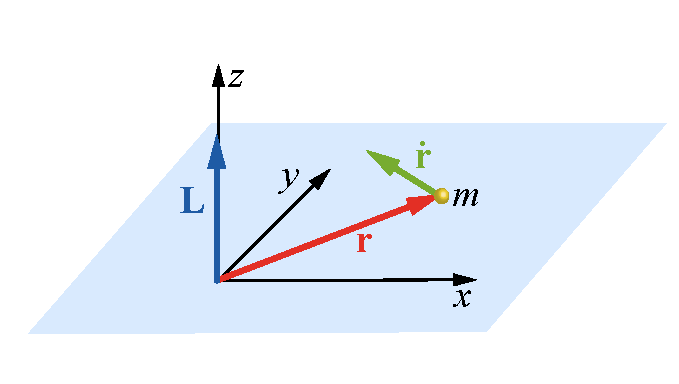
\includegraphics[width=0.5\textwidth]{Def_Drehimpuls.pdf}}
\hspace{\fill}
\rightfigure{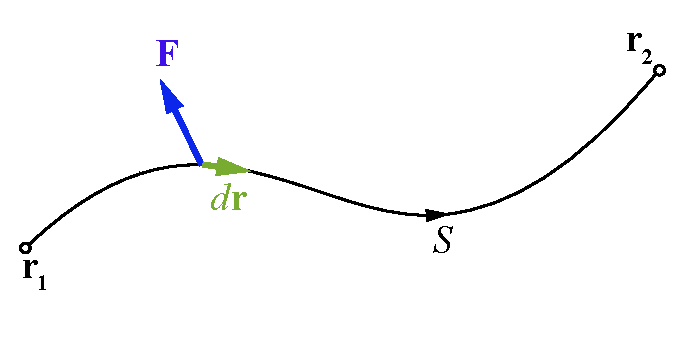
\includegraphics[width=0.5\textwidth]{Def_Arbeit.pdf}}
\leftcaption[Zur Definition des Drehimpulses eines Massepunktes.]{Zur Definition des Drehimpulses eines Massepunktes.
Im Bild wurde die Ebene, die durch die Vektoren $\vec{r}$ und $\dot{\vec{r}}$ aufgespannt wird, als $x$-$y$-Ebene gew�hlt, der Drehimpuls zeigt dann in $z$-Richtung (Rechte-Hand-Regel).}\label{abb:bew_Def_Drehimppuls}
\rightcaption[Zur Definition der Arbeit entlang eines Weges.]{Zur Definition der Arbeit entlang eines Weges $S$.}\label{abb:bew_Def_Arbeit}
\end{minipage}
\end{figure}

\subsubsection{Arbeit, Leistung und Energie}\label{kap:bew_arbeit_und_energie}

\subparagraph{\textbf{Arbeit}}\index{Arbeit}

Wir starten von der Newtonschen Bewegungsgleichung \eqref{eq:bew_NewtonBGL} und nehmen $m = \con$ an, woraus die allgemein �bliche Bewegungsgleichung 
\begin{align}
	m \ddot{\vec{r}} = \vec{F}(\vec{r},\dot{\vec{r}},t) \label{eq:bew_NewtonBGL2}
\end{align}
folgt.
Aus der Erfahrung ist bekannt, dass \anf{Arbeit} n�tig ist, um einen K�rper gegen eine Kraft zu bewegen: 
\begin{align}
	\delta W = - \vec{F} \: \mathrm{d}\vec{r} \label{eq:bew_Arbeit_infinitesimal}\,.
\end{align}
Hier ist $\delta W$ die Arbeit, die geleistet werden muss um einen Massepunkt in einem Kraftfeld $\vec{F}$ von $\vec{r}$ nach $\vec{r} + \mathrm{d}\vec{r}$ zu bewegen. 
F�r eine Bewegung entgegen der Kraft ist $ \vec{F} \cdot \D\vec{r} < 0$ und daher $\delta W > 0$, \dh es muss Arbeit aufgewendet werden, im umgekehrten Fall \anf{leistet} das Kraftfeld Arbeit.
Die gesamte geleistete Arbeit f�r eine Bewegung vom Ort $\vec{r_1}$ zum Ort $\vec{r_2}$ entlang eines Weges $S$ ist dann
\begin{align}
	W = \int\limits_{S} \delta W \mathrm{d}\vec{r} = -\int\limits_{S} \vec{F}(\vec{r},\dot{\vec{r}},t) \: \mathrm{d}\vec{r}\,.\label{eq:bew_Arbeit_total}
\end{align}
Das Integral in \eqref{eq:bew_Arbeit_total} ist ein Kurvenintegral und kann �ber eine Parametrisierung von $\vec{r}$ entlang des Weges berechnet werden, wie in \figref{bew_Def_Arbeit} dargestellt.
Dies bedeutet letztlich nichts anderes, als dass die Arbeit im Allgemeinen vom Weg abh�ngt, und dass die gr��te Arbeit wegen des Skalarproduktes in Richtung des Kraftfeldes verrichtet wird.
Kann man aber die infinitesimale Arbeit $\delta W = - \vec{F} \: \mathrm{d}\vec{r}$ als totales Differential $\mathrm{d} W $ schreiben, so gilt
\begin{align*}
	\gradv W = - \vec{F}(\vec{r})\,.
\end{align*}
Sowohl die Arbeit als auch die Kraft d�rfen dann nur vom Ort abh�ngen.
Eine solche Kraft nennt man \glslink{konservkr}{konservativ} und die entsprechende Arbeit auch potentielle Energie\index{Energie!potentielle} oder \glslink{potential}{\pot} $U$ des Kraftfeldes $\vec{F}(\vec{r})$. Man schreibt dann:
\begin{align}
	\vec{F}(\vec{r}) = -\gradv U(\vec{r}) \,.\label{eq:bew_konservative_Kraft}
\end{align}
In \probref{bew_konserv_Kraft} werden neben der Beziehung
\eqref{eq:bew_konservative_Kraft} auch einige andere Eigenschaften
des konservativen Kraftfeldes hergeleitet.

\subparagraph{\textbf{Leistung}}\index{Leistung}

Im Weiteren gehen wir von einem zeitunabh�ngigen Kraftfeld aus.
In diesem wird die geleistete Arbeit pro Zeiteinheit als Leistung definiert und kann wie folgt geschrieben werden:
\begin{align}
	P = \frac{\mathrm{d} W}{\mathrm{d}t} = - \dot{\vec{r}} \:\vec{F} = - \vec{v} \: \vec{F}\,. \label{eq:bew_Def_Leistung}
\end{align}

\subparagraph{\textbf{Energie und Energieerhaltung}}\index{Energie}\index{Energieerhaltung}

Die kinetische Energie wird definiert als
\begin{align}
	T = \frac{m}{2} \: \dot{\vec{r}}^2\,. \label{eq:bew_Def_kinEnergie}
\end{align}
Die Zeitableitung von \eqref{eq:bew_Def_kinEnergie} ergibt
	\[\frac{\mathrm{d} T}{\mathrm{d}t} = m \ddot {\vec{r}}\:\dot{\vec{r}} = \vec{F}\:\dot{\vec{r}} = - P\,.
\]
Integration �ber $t$ ergibt
	\[W_{2,1} = \int\limits_{t_1}^{t_2} \mathrm{d}t P(t)  = - \int\limits_{t_1}^{t_2} \mathrm{d}t \frac{\mathrm{d} T}{\mathrm{d}t} = T_1 -T_2\,.
\]
Die geleistete Arbeit entspricht also der �nderung der kinetischen Energie.
In einem konservativen Kraftfeld h�ngt die Arbeit nicht vom Weg ab, sondern nur von der potentiellen Energie $U$ am Anfangs- und Endpunkt, es gilt also
	\[T_1 + U_1 = T_2 + U_2\,.
\]
In einem konservativen Kraftfeld ist daher die Gesamtenergie konstant: 
\begin{align}
E = T + U = \frac{m}{2} \:\dot{\vec{r}}^2 + U(\vec{r}) = \con\,. \label{eq:bew_EnergieSatz}
\end{align}
Gleichung \eqref{eq:bew_EnergieSatz} ist der Energieerhaltungssatz der Mechanik f�r konservative Kr�fte.

\subsection{Transformation des Bezugssystems, Scheinkr�fte}\index{Scheinkraft|textbf}\index{Tr�gheitskraft|textbf}\index{Kraft!Schein-}\label{kap:bew_trafo_bezugssystem}

Physikalische Vorg�nge laufen unabh�ngig von der Wahl des KOS ab. Wir wollen Koordinatensysteme jeweils mit einem $\vec{\Sigma}$ bezeichnen.
Die Auswahl eines Bezugs- \bzw Koordinatensystems erfolgt dabei \ia so, dass sich das physikalische Problem durch m�glichst einfache Gleichungen beschreiben l�sst.

Aus dem ersten Axiom folgt die Existenz von Inertialsystemen\index{Inertialsystem}, in denen kr�ftefreie K�rper entweder ruhen oder sich mit konstanter Geschwindigkeit $\vec{v}$ bewegen.
Wir wollen nun alle denkbaren Inertialsysteme der Newtonschen Mechanik finden und auch kl�ren, wann durch den Wechsel eines Bezugssystems kein Inertialsystem mehr vorliegt.
Dabei benutzen wir der Einfachheit halber kartesische Koordinaten zu einem beliebigen Zeitpunkt $t$.
Dann kann die Umrechnung von einem Ausgangsbezugssystem $\vec{\Sigma}$ in ein anderes Bezugssystem $\vec{\Sigma}'$, in welchem wir die Koordinaten mit gestrichenen Gr��en ($\vec{r}', \vec{v}'$ usw.) beschreiben, durch eine Kombination von Translationen und Rotationen beschrieben werden. 

\subsubsection{Galilei-Transformation}\index{Transformation!Galilei-} \label{kap:bew_Galilei_Trafo}

Wir betrachten zun�chst Translationen\index{Translation} (\figref{bew_Galilei_Trafo}) und nehmen an, dass zum Zeitpunkt $t\!=\!0$ die Bezugssysteme $\vec{\Sigma}$ und $\vec{\Sigma}'$ identisch sind und keine Kr�fte wirken. 
Im Inertialsystem $\vec{\Sigma}$ gilt dann $m \ddot{\vec{r}}\! = \!0$. 
Das transformierte Bezugssystem $\vec{\Sigma}'$ geht aus dem urspr�nglichen Bezugssystem $\vec{\Sigma}$ durch eine Verschiebung $\vec{R}(t)$ hervor. 
Damit $\vec{\Sigma}'$ auch ein Inertialsystem ist, \dh der Massepunkt auch bez�glich dieses Bezugssystems ruht oder sich mit konstanter Geschwindigkeit bewegt, muss gelten $m \ddot{\vec{r}}'\! =\! 0$. 
Nach \figref{bew_Galilei_Trafo} ist aber $\vec{r} \!= \!\vec{r}' + \vec{R}(t) $, woraus folgt: $m \ddot{\vec{r}}' \!= \!m \ddot{\vec{r}} - m \ddot{\vec{R}}$. 
Dies ist nur dann gleich Null, wenn $\ddot{\vec{R}}\!=\!0$ ist, woraus folgt: $\dot{\vec{R}}\!=\!\vec{V} \!=\! \vec{const} $ und damit $\vec{R}\! = \!\vec{V} \:t$. 
Hierbei ist $\vec{V}$ die Relativgeschwindigkeit der Translation der beiden Bezugssysteme. 

\begin{figure}
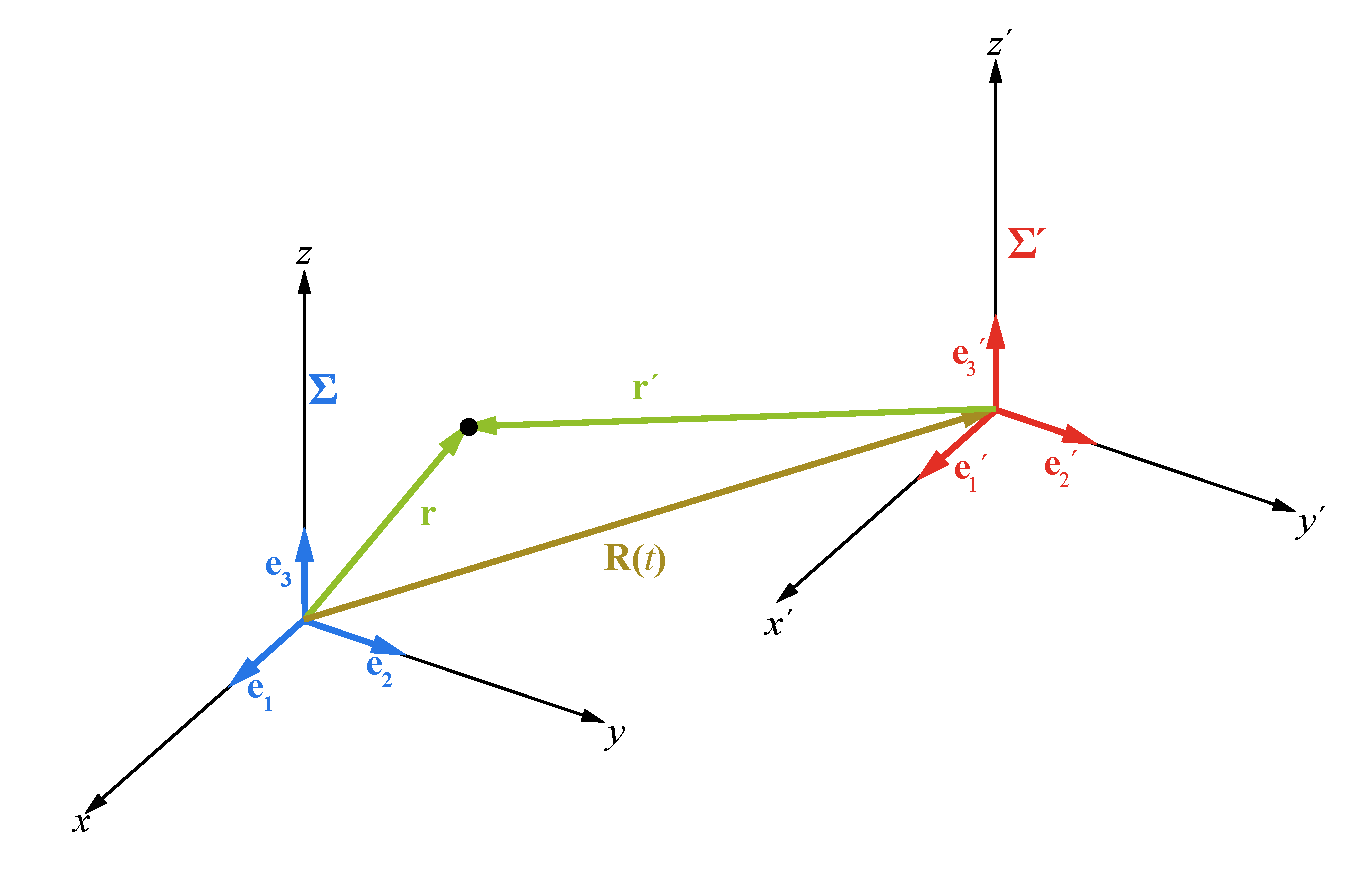
\includegraphics[width=\textwidth]{Galilei_Trafo.pdf}%
\caption[Verschiebungen zwischen Koordinatensystemen.]{Verschiebungen zwischen Koordinatensystemen. F�r die Galilei-Transformation gilt $\dot{\vec{R}}\!=\!\vec{V} \!=\! \text{const} $.}
\label{abb:bew_Galilei_Trafo}
\end{figure}

F�r die Zeit gilt in der Newtonschen Mechanik $t' = t$, sodass wir zusammenfassend formulieren k�nnen, dass man durch Translation genau dann wieder ein Inertialsystem erh�lt, wenn sich das Bezugssystem $\vec{\Sigma}'$ mit konstanter Relativgeschwindigkeit $\vec{V}$ zum Inertialsystem $\vec{\Sigma}$  bewegt.
Es gelten dann die \emph{Galilei-Transformationen}: 
\begin{align}
	\vec{r}' = \phantom'\vec{r} - \vec{V}\:t \quad \text{und} \quad t' = \phantom't\,. \label{eq:Bew_Galilei_Trafo}
\end{align}

Das zweite Newtonsche Axiom bleibt unter Galilei-Transformationen unver�ndert, die Newtonschen Bewegungsgleichungen
�ndern ihre Form beim �bergang zwischen Inertialsystemen nicht.\footnote{Selbstverst�ndlich d�rfen Inertialsysteme auch um eine beliebige Achse gegeneinander rotiert oder um einen konstanten Vektor verschoben sein. Auch darf der Zeitnullpunkt anders gew�hlt werden. Diese allgemeine Form der Galilei-Transformation ben�tigen wir hier jedoch nicht und wir beschr�nken uns daher auf die einfache Form aus Gleichung \eqref{eq:Bew_Galilei_Trafo}.}\\
Galilei-Transformationen sind die allgemeinsten Transformationen
zwischen Inertialsystemen der Newtonschen Mechanik.%
\footnote{In der relativistischen Physik l�sst man die Bedingung $t' = t$
fallen und kommt dann zu anderen Transformationen zwischen den Inertialsystemen, den sogenannten Lorentz-Transformationen.}
Wir stellen nun noch die Frage, wie die Bewegungsgleichungen in den beiden Systemen aussehen, wenn im System $\vec{\Sigma}$ eine Kraft $\vec{F} = m \ddot{\vec{r}}$ auf den Massepunkt wirkt und das System $\vec{\Sigma}'$ sich beliebig, \zb auch beschleunigt gegen�ber $\vec{\Sigma}$ bewegt.
Durch Einsetzen in die Galilei-Transformation erh�lt man $m \ddot{\vec{r}}' \!= \!m \ddot{\vec{r}}$, das zweite Axiom beh�lt also seine Form, wenn wir einfach $\vec{F} = \vec{F}'$ setzen. 
Wir m�ssen aber $\vec{F}'(\vec{r}',\dot{\vec{r}}')$ durch die transformierten Gr��en $\vec{r}',\dot{\vec{r}}'$ ausdr�cken, da die Kraft \ia von diesen Gr��en abh�ngt. 
Wir benutzen wieder $\vec{r}(t) \!= \!\vec{r}'(t) + \vec{R}(t)$, wobei diesmal $\vec{R}(t)$ beliebig zeitabh�ngig ist und erhalten
\begin{align}
	\vec{F}' \;=\; m \:\ddot{\vec{r}}' \;= \; m\: \ddot{\vec{r}} - m \ddot{\vec{R}}\;= \; \vec{F} - m \:\ddot{\vec{R}}\,.\label{eq:Bew_Galilei_Trafo_2}
\end{align}
Gleichung \eqref{eq:Bew_Galilei_Trafo_2} besagt, dass wir die Newtonsche Bewegungsgleichung auch in $\vec{\Sigma}'$ verwenden k�nnen, wenn wir zur Kraft $\vec{F}$ eine Scheinkraft\index{Scheinkraft}\index{Kraft!Schein}
$\vec{F}_\text{S} = - m \ddot{\vec{R}}$ addieren.
Scheinkr�fte sind im System $\vec{\Sigma}'$ sehr wohl real sp�r- und messbar und ergeben sich anders als die im \kap{bew_newton_axioms} beschriebenen Kr�fte nur aus der Wahl eines entsprechend bewegten Bezugssystems.\footnote{Der Begriff Scheinkraft kommt daher, dass eine solche eben f�r einen Beobachter im Inertialsystem nicht auftritt und f�r diesen somit "`scheinbar"' nicht existiert.} Wir werden im folgenden Kapitel sehen, dass auch rotierende Systeme\index{Rotation} keine Inertialsysteme mehr sind und daher in diesen ebenfalls Scheinkr�fte auftreten.


\subsubsection{Rotierende Systeme}\index{Bezugssystem!rotierendes} \index{Rotation} \label{kap:bew_rotating_systems}

\subparagraph{\textbf{Mathematische Beschreibung von Drehungen kartesischer KOS}}\index{Energie}\index{Drehung}\index{Koordinatensystem!kartesisches} \index{Drehmatrix}\index{Rotationsmatrix}

Nachdem wir zeitunabh�ngige und zeitabh�ngige Translationen von Koordinatensystemen betrachtet haben, wenden wir uns der Rotation (kartesischer) Koordinatensysteme zu, wobei wir als erstes die zeitunabh�ngige, \dh feste (Ver)Drehung zwischen zwei Koordinatensystemen betrachten wollen.
Dabei werden wir die elegante mathematische Beschreibung durch \emph{Drehmatrizen} (h�ufig auch Rotationsmatrizen genannt) kennen lernen.
Diese lassen sich herleiten, indem man ein neues gestrichenes Koordinatensystem $\vec{\Sigma}'$ aus einem (ungestrichenen) Koordinatensystem $\vec{\Sigma}$ durch Drehung um jeweils einen Winkel $\varphi$ um eine der $\vec{e}_i$-Achsen betrachtet.

\begin{figure}
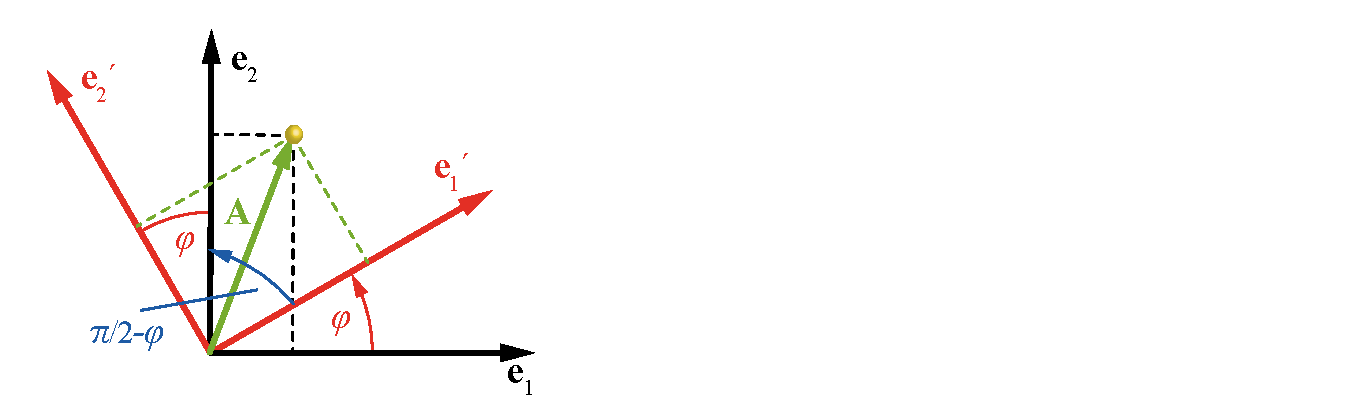
\includegraphics[width=\textwidth]{Drehmatrix.pdf}%
\caption[Zur Herleitung von Drehmatrizen.]{Zur Herleitung von Drehmatrizen. Dargestellt ist eine Drehung um die $\vec{e}_3$-Achse. Der Vektor $\vec{A}$ wird davon nicht ber�hrt, allerdings h�ngt seine Koeffizientendarstellung vom gew�hlten Koordinatensystem ab.}
\label{abb:bew_Drehmatrix}
\end{figure}

Aus \figref{bew_Drehmatrix} kann man ablesen, dass sich die $\vec{\Sigma}$-Basisvektoren zu den $\vec{\Sigma}'$-Basisvektoren folgenderma�en verhalten:\footnote{Wir bezeichnen hier die Basisvektoren allgemein mit $\vec{e}_1, \vec{e}_2, \vec{e}_3$, wobei f�r ein kartesisches \KOS $\vec{e}_1 = \veceX, \vec{e}_2 = \veceY, \vec{e}_3 = \veceZ$ gilt.}
\begin{align}
	\vec{e}_i{}' &= (\vec{e}_i{}' \cdot \vec{e}_1)\, \vec{e}_1 + (\vec{e}_i{}' \cdot \vec{e}_2)\, \vec{e}_2 = \vec{e}_i{}' = a_{i1}\,\vec{e}_1 + a_{i2}\,\vec{e}_2 \,, \label{eq:bew_Drehmatrix1_2D} 
\end{align}
\bzw verallgemeinert f�r den dreidimensionalen Fall
\begin{align}
\begin{split}
	\vec{e}_i'{} &= (\vec{e}_i{}'\cdot \vec{e}_1)\, \vec{e}_1 + (\vec{e}_i{}'\cdot \vec{e}_2)\, \vec{e}_2 + (\vec{e}_i{}'\cdot \vec{e}_3)\,\vec{e}_3\,,\\
	\vec{e}_i{}'&= a_{i1}\,\vec{e}_1 + a_{i2}\,\vec{e}_2  + a_{i3}\, \vec{e}_3\,.  
\end{split} \label{eq:bew_Drehmatrix1}
\end{align}
Die $a_{ij} = \vec{e}_i{}'\cdot \vec{e}_j$ hei�en Richtungskosinus\index{Richtungskosinus}.
F�r den Fall in \figref{bew_Drehmatrix} ergibt sich beispielsweise $\vec{e}_1{}' \cdot \vec{e}_1 = \cos \varphi\,$ und $\,\vec{e}_1{}' \cdot \vec{e}_2 = \cos {(\pi/2 - \varphi)} =
+ \sin{\varphi}\,$. Allgemein kann man die Transformation des Vektors $\vec{A}$ schreiben als:
\begin{align}
	\vec{A}' = \phantom'\mathbb{R} \: \vec{A} = \begin{pmatrix} a_{11} & a_{12} & a_{13} \\ a_{21} & a_{22} & a_{23} \\ a_{31} & a_{32} & a_{33} \end{pmatrix}\, \vec{A}\,.
\end{align}
Die Drehung um die $z$-Achse ($\vec{e}_3$) um einen positiven Winkel $\varphi$ (siehe \figref{bew_Drehmatrix}, Drehung entgegengesetzt zum Uhrzeigersinn) ist dann beispielsweise durch die Drehmatrix $\mathbb{R}_z(\varphi)$ beschrieben:
	\[\mathbb{R}_z(\varphi) \: = \;\begin{pmatrix} +\cos\varphi & +\sin\varphi & 0 \\ -\sin\varphi & +\cos\varphi & 0 \\ 0 & 0 & 1 \end{pmatrix}\,.
\]
Wir werden diese Drehmatrizen ausgiebig nutzen, insbesondere in der Himmelsmechanik und in der Mechanik starrer K�rper.

\subparagraph{\textbf{Dynamik in rotierenden Koordinatensystemen}}\index{Energie}

Wir wollen nun zeitabh�ngige Drehungen betrachten und zwei KOS $\vec{\Sigma}$ und $\vec{\Sigma}'$ gegeneinander rotieren lassen. 
Diese sollen f�r $t = 0$ �berein stimmen und f�r alle weiteren Zeiten $t$ ihren gleichen Koordinatenursprung behalten. 
Das System $\vec{\Sigma}$ sei dabei ein Inertialsystem und durch die Basis-Einheitsvektoren $\vec{e}_i$ mit $i=1\ldots3$ gegeben,
das rotierende System $\vec{\Sigma}'$ entsprechend durch die Vektoren $\vec{e}_i{}'$. 
Dabei nehmen wir an, dass nur das System $\vec{\Sigma}'$ von der Zeit abh�ngt.
Wir betrachten nun einen Vektor, der im rotierenden System $\vec{\Sigma}'$ (\figref{bew_Rot_KOS}) durch $\vec{A}'(t)$  beschrieben wird und dessen zeitliche Ver�nderung gegeben sei durch:
%\footnote{An dieser Stelle sei unterschieden zwischen dem Vektor an sich (der physikalischen Gr��e) $\vec{\mathcal{A}}$ und seiner Beschreibung $\vec{A}$ bzw. $\vec{A'}$ im jeweiligen Koordinatensystem. Eine physikalische Gr��e, z.B. $\vec{\mathcal{A}}$, muss nat�rlich immer gleich sein, unabh�ngig in welchem System man sich befindet. Im Folgenden werden wir diese Unterscheidung weglassen und einfach  $\vec{A}$ bzw. $\vec{A'}$ schreiben.}
\begin{align*}
	\frac{\D \vec{A'}}{\D t} = \frac{\D A_1'}{\D t} \:\vecpex + \frac{\D A_2'}{\D t} \:\vecpey + \frac{\D A_3'}{\D t} \:\vecpez\,.
\end{align*}
Wollen wir die zeitliche Entwicklung im Inertialsystem berechnen, m�ssen wir noch ber�cksichtigen, dass die Einheitsvektoren $\vec{e}_i$ von der Zeit abh�ngen und wir deshalb ihre zeitliche Ableitung berechnen m�ssen, also:
\begin{align*}
	\frac{\D \vec{A}}{\D t} = \frac{\D \vec{A'}}{\D t} + A_1' \: \dvecepx + A_2' \: \dvecepy + A_3' \: \dvecepz\,.
\end{align*}

\begin{figure}
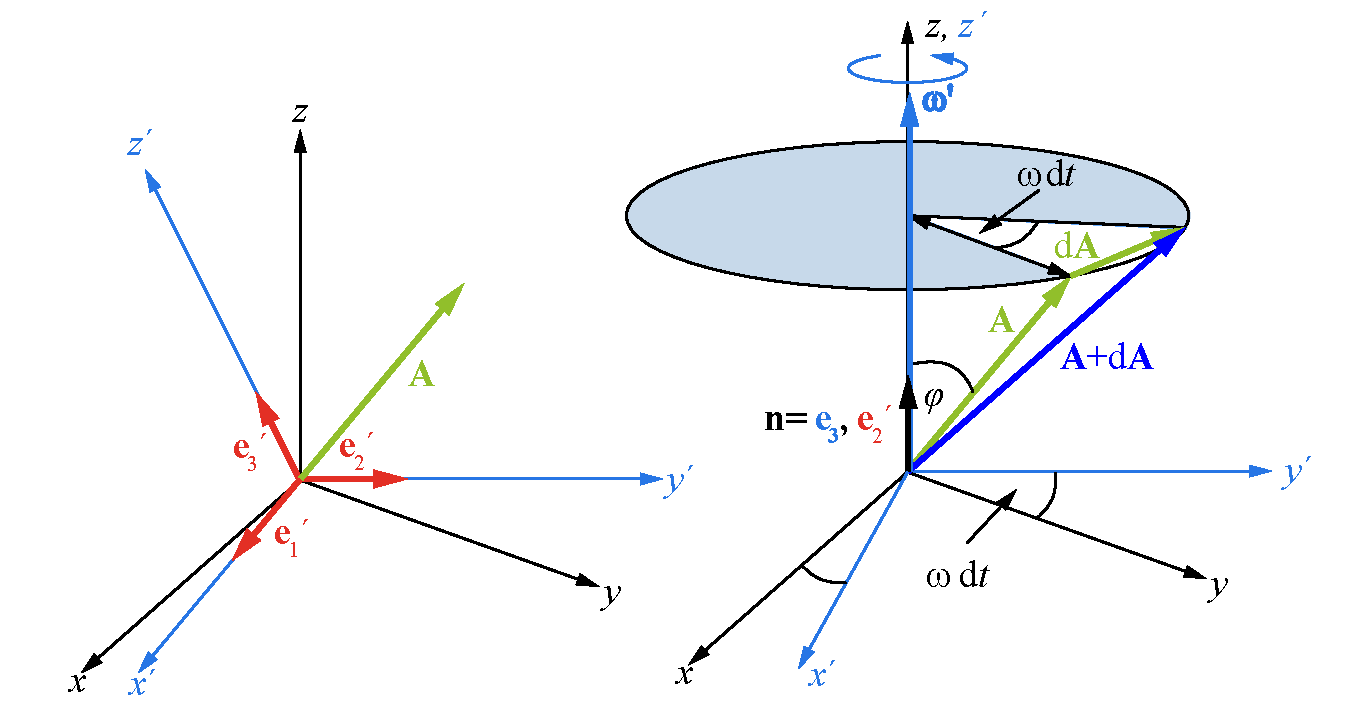
\includegraphics[width=\textwidth]{Rot_KOS.pdf}%
\caption[Rotierende Bezugssysteme.]{Rotierende Bezugssysteme. In beiden Bildern haben wir vereinfachend angenommen, dass die Nullpunkte von $\vec{\Sigma}$ und $\vec{\Sigma} '$ �bereinstimmen. Im rechten Bild nehmen wir zudem an, dass die Drehachse $\vec{n}$ sowohl mit der $z$-Achse als auch der $z'$-Achse �bereinstimmt und fest im Raum steht. $\vec{A}$ ist ein beliebiger Vektor.}%
\label{abb:bew_Rot_KOS}
\end{figure}

Wir m�ssen als n�chstes die ${\dot{\vec{e}}_i}{}'$ bestimmen, \dh herausfinden, wie sich die Einheitsvektoren ${\vec{e}_i}{}'$ aus Sicht von $\vec{\Sigma}$ �ndern.
Wir beschreiben dazu die Rotation von $\vec{\Sigma}'$ um eine Drehachse $\vec{n}$ mit dem Vektor der Winkelgeschwindigkeit $\vec{\omega}$ (\figref{bew_Rot_KOS}). 
Sowohl $\vec{n}$ als auch $\vec{\omega}$ k�nnen \ia zeitabh�ngig sein.
Unter Benutzung der Orthogonalit�tsrelationen der Einheitsvektoren ${\vec{e}_i}{}'$ findet man (in (\probref{bew_Rot_System}) im Detail ausgef�hrt) folgende Beziehung:
\begin{align}
	 A_1' \, \dvecepx + A_2' \,\dvecepy + A_3 \, \dvecepz \:&=\: \vec{\omega}' \times \vec{A}' \quad \rightarrow\ \quad 
	\frac{\mathrm{d} \vec{A}}{\D t}\: =\: \frac{\D \vec{A'}}{\D t} + \:\vec{\omega}' \times \vec{A}'\,. \label{eq:bew_Rot_System1}
\end{align}
Wir verweisen auf  \figref{bew_Rot_KOS}, in der wir den speziellen Fall dargestellt haben, bei welchem die Drehachse mit den $z$-\, und der $z'$-Achsen der beiden Koordinatensysteme zusammenf�llt. 
Wir k�nnen \eqref{eq:bew_Rot_System1} als allgemeine Transformation der Zeitableitung zwischen den beiden gegeneinander rotierenden Systemen formulieren:
\begin{align}
  % better no \mathclap here
	\underbrace{\lk \frac{\mathrm{d} \vec{A}} {\mathrm{d} t} \rk}_{\text{Ableitung in } \:\Sigma}\:
	&=\; \underbrace{\lk \frac{\mathrm{d} \vec{A}'} {\mathrm{d} t} \rk}_{\text{Ableitung in}\: \Sigma '} 
	+ \:~~\underbrace{\vec{\omega}' \times \vec{A}'}_{\text{Zusatzterm}} 
	~~=~~ \underbrace{\left\{\frac{\mathrm{d}}{\mathrm{d} t} + \vec{\omega}' \times \right\}}_{\text{Operator}} \vec{A}'~. \label{eq:bew_Rot_System2}
\end{align}
Wir weisen darauf hin, dass $\vec{\omega}'$ der Rotationsvektor ist, wie er im gestrichenen Inertialsystem $\vec{\Sigma}'$ vorliegt.
In diesem ist die Orientierung der Drehachse im Allgemeinen verschieden von der in $\vec{\Sigma}$, wie wir in \kap{bew_Coriolis-Kraft}  und den �bungen zeigen werden.\footnote{Ein Beispiel ist der Vektor der Rotationsgeschwindigkeit der Erde, der an den Polen senkrecht auf der Erdoberfl�che steht, am �quator dagegen parallel zur Erdoberfl�che.} 
Um die Transformation f�r die zweite Zeitableitung zu erhalten, wenden wir auf \eqref{eq:bew_Rot_System2} den Operator $\left\{\D / \D t  + \vec{\omega}' \times \right\}$ noch einmal an und erhalten (\probref{bew_Rot_System})
\begin{align}
	\frac{\mathrm{d^2} {\vec{A}}}{\mathrm{d} t^2} &= \frac{\mathrm{d^2} \vec{A'}}{\mathrm{d} t^2} + \:\dot{\vec{\omega}}' \times \vec{A}' + \: 2 \vec{\omega '}\times \dot{\vec{A}}'  + \:\vec{\omega'}\times( \vec{\omega '} \times \vec{A'})\,. \label{eq:bew_Rot_System3}
\end{align}
Wir k�nnen nun f�r den beliebigen Vektor $\vec{A}$ den Ortsvektor $\vec{r}$ einsetzen und erhalten
\begin{align}
	\ddot{\vec{r}} &= \ddot{\vec{r}}' + \: \dot{\vec{\omega}}' \times \vec{r'} +  \: 2 \vec{\omega}' \times \dot{\vec{r}}'  + \:\vec{\omega '}\times( \vec{\omega '} \times \vec{r'})\,. \label{eq:bew_Rot_System4}
\end{align}
Multipliziert man \eqref{eq:bew_Rot_System4} mit $m$ und fasst die Kraft $m \ddot{\vec{r}}$ im Inertialsystem $\vec{\Sigma}$ als eine externe Kraft $\vec{F}^\text{(ext)}$ auf (\zb als eine der weiter oben genannten Kr�fte wie Gravitations- oder Coulomb-Kraft), dann kann man wegen $\vec{F}^\text{(ext)} = \vec{F'}^\text{(ext)}$ die Bewegungsgleichung folgenderma�en schreiben:
\begin{align}
	\ddot{\vec{r}}' &= \frac{\vec{F}^\text{(ext)}}{m} - \: \dot{\vec{\omega}}' \times \vec{r}' - \: 2 \vec{\omega '}\times \dot{\vec{r}}'  - \:\vec{\omega}' \times( \vec{\omega}' \times \vec{r}')\,. \label{eq:bew_Rot_System5}
\end{align}
Gleichung \eqref{eq:bew_Rot_System5} ist die Erweiterung des zweiten Newtonschen Axioms auf rotierende KOS, bei denen die Ursprungskoordinaten zusammenfallen (\figref{bew_Rot_KOS}).
Wir wollen diese Beschr�nkung jetzt fallen lassen und auch eine Verschiebung $\vec{R}(t)$ des KOS zulassen.
Uns interessiert nun das Transformationsverhalten des Vektors  $\vec{r}'(t) = \vec{r}(t) - \vec{R}(t)$.
Dabei ist $\vec{r}$ der Ort des betrachteten Massepunktes relativ zum Nullpunkt in $\vec{\Sigma}$ und $\vec{r}'(t)$ derselbe Vektor vom Nullpunkt in $\vec{\Sigma} '$ aus gesehen.
Aus der zweiten Zeitableitung von $\vec{r}(t)$ nach der Bildungsvorschrift \eqref{eq:bew_Rot_System1} und \eqref{eq:bew_Rot_System3} folgt dann die Erweiterung des zweiten Newtonschen Axioms auf rotierende und linear beschleunigte Bezugssysteme:
\begin{align}
		 m \ddot{\vec{r}}' &= \vec{F}^\text{(ext)} - m \,\ddot{\vec{R}}' - m\, \dot{\vec{\omega}}' \times \lk \vec{r}' - \vec{R}' \rk - 2 m\, \vec{\omega}' \times \lk \dot{\vec{r}}' - \dot{\vec{R}}' \rk - m\, \vec{\omega}' \times \lek \vec{\omega}' \times \lk \vec{r}' - \vec{R'} \rk \rek\,, \\
		 m \ddot{\vec{r}}' &= \vec{F}^\text{(ext)} + \vec{F'}_\text{bT} + \vec{F'}_\text{bR} +\vec{F'}_\text{Cor} + \vec{F'}_\text{Z}\,.\label{eq:bew_Rot_System6}
\end{align}
Formel \eqref{eq:bew_Rot_System6} ist die Bewegungsgleichung f�r einen Massepunkt am Ort $\vec{r}'$ in einem mit $\vec{\omega}'$ rotierenden Bezugssystem $\vec{\Sigma}'$, auf den �u�ere Kr�fte $\vec{F}^\text{(ext)}$ und Scheinkr�fte wirken.
Der Verbindungsvektor $\vec{R}'$ zeigt dabei vom Ursprung des rotierenden Bezugssystems $\vec{\Sigma} '$ zum Drehzentrum.
Gleichung \eqref{eq:bew_Rot_System6} geht f�r $\vec{\omega}' = 0$ und $\ddot{\vec{R}}' = 0$ in die Form f�r Inertialsysteme �ber.
Umgekehrt wird auch ein kr�ftefreier K�rper $(\vec{F}^\text{(ext)} = 0)$ aus der Sicht eines Beobachters in einem allgemein beschleunigten und rotierenden Bezugssystem durch Scheinkr�fte beschleunigt, bleibt also nicht in Ruhe oder gleichf�rmiger Bewegung.
Alle Scheinkr�fte sind proportional zur (tr�gen) Masse und in rotierenden Systemen (mit Ausnahme von $\vec{F'}_\text{bl}$) zu $\vec{\omega}'$ \bzw $\dot{\vec{\omega}}'$.
Im Einzelnen sind das nach \eqref{eq:bew_Rot_System6}:
\begin{enumerate}
	\item Scheinkraft durch beschleunigte Translation von $\vec{\Sigma} '$ gegen�ber $\vec{\Sigma}$ (vgl. \eqref{eq:Bew_Galilei_Trafo_2}):
\begin{align} 
		\vec{F'}_\text{bT} = - m \ddot{\vec{R}}'\,. \label{eq:bew_beschl_Kraft}
\end{align}
	\item Euler-Kraft\index{Euler-Kraft}\index{Kraft!Euler-}\footnote{Leonhard Euler\indexp{Euler, Leonhard} (1707--1783) war einer der bedeutendsten Mathematiker des 18.\ Jahrhunderts. Der in der Schweiz geborene Euler, der vor allem in Berlin und St.~Petersburg forschte, war aber auch in der Physik und Astronomie t�tig und machte zahlreiche Entdeckungen in diesen Bereichen. In der Mathematik sind vor allem seine Beitr�ge zur Infinitesimalrechnung und der Graphentheorie zu nennen. In der Physik waren \ua seine Arbeiten in der Mechanik und Str�mungsdynamik wegweisend. Obwohl er bereits 1771 erblindete, war er weiterhin einer der brillantesten und produktivsten Mathematiker aller Zeiten. Eulers Arbeiten inspirierten viele Generationen von Mathematikern nachhaltig.} -- Scheinkraft durch beschleunigte Rotation von $\vec{\Sigma} '$ gegen�ber $\vec{\Sigma}$:
\begin{align} 
		\vec{F'}_\text{bR} = - m \dot{\vec{\omega}}' \times \lk \vec{r'} -\vec{R}' \rk\,. \label{eq:bew_beschl_Rotation}
\end{align}
	\item Coriolis-Kraft\index{Kraft!Coriolis-}\footnote{Gaspard Gustave de Coriolis\indexp{Coriolis, Gaspard Gustave@de Coriolis, Gaspard Gustave} (1792--1843) war ein franz�sischer Mathematiker und Physiker, der die sp�ter nach ihm benannte Coriolis-Kraft als Scheinkraft eines in einem rotierenden System bewegten K�rpers untersuchte. Au�erdem ver�ffentlichte Coriolis Arbeiten zur Wirtschaftsmathematik. Verschiedentlich wird auch Euler als Entdecker der Coriolis-Kraft genannt \cite{Grimsehl1977}.}:
\begin{align} 
		\vec{F'}_\text{Cor} = - 2 m \vec{\omega}' \times \lk \dot{\vec{r}}' - \dot{\vec{R}}' \rk\,. \label{eq:bew_Coriolis_Kraft}
\end{align}
	\item Zentrifugalkraft\index{Kraft!Zentrifugal-}:
\begin{align} 
		\vec{F'}_\text{Z} = - m \vec{\omega}' \times \lek \vec{\omega}' \times \lk \vec{r}' - \vec{R}' \rk \rek\,.\label{eq:bew_Zentrifugal_Kraft}
\end{align}
\end{enumerate} 
Wir fassen die Erkenntnisse zur Bewegung in linear beschleunigten und rotierenden Bezugssystemen zusammen:\\
Das zweite Newtonsche Axiom gilt in seiner in \eqref{eq:bew_NewtonBGL} definierten Form \emph{nur} in Inertialsystemen.
Es kann aber auch in Nichtinertialsystemen formuliert werden (Gleichungen \eqref{eq:bew_Rot_System5} und \eqref{eq:Bew_Galilei_Trafo_2}), wobei dann zus�tzliche Terme zu ber�cksichtigen sind.
Diese zus�tzlichen Terme sind die sogenannten Scheinkr�fte oder Tr�gheitskr�fte\index{Scheinkraft}\index{Tr�gheitskraft}, zu denen in rotierenden Bezugssystemen insbesondere die Zentrifugal- und die Coriolis-Kraft geh�ren.
Scheinkr�fte sind f�r einen Beobachter im mitbewegten Koordinatensystem reale Kr�fte, die allein durch die Transformation in das Nichtinertialsystem auftreten und ihren physikalischen Ursprung in der Tr�gheitskraft $m \ddot{\vec{r}}$ haben.
Das Auftreten von Scheinkr�ften ist damit immer auch ein Indiz daf�r, dass das Bezugssystem kein Inertialsystem ist. \\

%BEISPIEL 1 %%%%%%%%%%%%%%%%%%%%%%%%%%%%%%%%%%%%%%%%%%%%%%%%%%%%%%%%%%%%%%%%%%%%%%%%%%%%%%%%%%
\begin{example}{Scheinkr�fte}\\
\smallskip
An dieser Stelle wollen wir vor einem h�ufigen Fehler warnen.
Die Zentrifugalkraft $\vec{F'_\text{Z}}$ \eqref{eq:bew_Zentrifugal_Kraft} ist nicht die nach dem dritten Axiom auftretende Gegenkraft zur Radialkraft\index{Kraft!Radial-} $\vec{F}_r$ (oft auch Zentripetalkraft\index{Kraft!Zentripetal-} genannt), die einen K�rper auf eine Kreisbahn oder allgemein zur Rotation zwingt.
Das erkennt man schon daran, dass die beiden Kr�fte in unterschiedlichen Bezugssystemen definiert sind und dass sie an demselben K�rper angreifen und nicht wie im dritten Axiom gefordert an zwei verschiedenen K�rpern.
Wir wollen das an zwei Beispielen verdeutlichen:
\begin{itemize}
	\item \emph{Sitz auf einem Kettenkarusell}
	\begin{itemize}
		\item Im System $\vec{\Sigma}$: Radialkraft auf Karussellsitz (externe Kraft) und Spannung in Aufh�ngungskette (Gegenkraft)
		\item Im System $\vec{\Sigma}'$: Zentrifugalkraft auf Sitz (Scheinkraft)
	\end{itemize}
	\item \emph{Satellit in der Erdumlaufbahn}
	\begin{itemize}
		\item Im System $\vec{\Sigma}$: Gravitationskraft von Erde auf Satellit (externe Kraft) und Gravitationskraft von Satellit auf Erde (Gegenkraft)
		\item Im System $\vec{\Sigma}'$: Zentrifugalkraft (Scheinkraft)
	\end{itemize}
\end{itemize}
Die Scheinkr�fte haben keine Gegenkr�fte, die dem dritten Axiom gen�gen.
F�r die Bedingung der Ruhe bzw. gleichf�rmigen Bewegung im Bezugssystem $\vec{\Sigma} '$ kann aber sehr wohl eine Scheinkraft nach dem zweiten Newtonschen Axiom gleich einer extern wirkenden Kraft sein.
\label{bsp:Scheinkraefte}
\end{example}
%BEISPIEL %%%%%%%%%%%%%%%%%%%%%%%%%%%%%%%%%%%%%%%%%%%%%%%%%%%%%%%%%%%%%%%%%%%%%%%%%%%%%%%%%%

Wir haben das Thema der Bewegungsgleichungen in den Nichtinertialsystemen etwas ausf�hrlicher behandelt, da es in unseren �bungen eine gro�e Rolle spielen wird. 
H�ufig findet man eine unsaubere Beschreibung von solchen rotierenden Systemen durch nicht korrekte Ber�cksichtigung des jeweiligen Bezugssystems. Wir wollen daher in \kapitel{bew_anwendungen_I} und in den �bungen die Scheinkr�fte Zentrifugalkraft und Coriolis-Kraft am Beispiel der rotierenden Erde intensiv diskutieren. Zuvor aber betrachten wir noch die Mechanik von mehreren Massepunkten.

\subsection{Mechanik von Massepunktsystemen}\label{kap:bew_system_massepunkt}

\subsubsection{Schwerpunkt, Gesamtgr��en und Erhaltungss�tze}\index{Schwerpunkt} \index{Erhaltungss�tze} \label{kap:bew_basics_of_systems}

Wir erweitern das Konzept des Massepunktes auf Systeme, die aus vielen Teilchen bestehen.
Die Kr�fte, die auf jedes dieser Teilchen wirken, k�nnen zerlegt werden in
\begin{itemize}
	\item \emph{innere Kr�fte}\index{Kraft!innere}, die paarweise zwischen den Massepunkten wirken.
          Die Kraft, die $m_i$ auf $m_{\kern -1ptj}$ aus�bt, ist $\vec{F}_{\kern-2ndji}$\footnote{Hier bezeichnen $i,j$ Teilchen und keine r�umlichen Komponenten wie in \kapitel{bew_trafo_bezugssystem}.}. Nach dem dritten Axiom wirkt aber auch $\vec{F}_{\kern-1ndi\kern-1ptj}$ von $m_{\kern -1ptj}$ auf $m_i$. 
	\item \emph{�u�ere Kr�fte}\index{Kraft!�u�ere}, die von au�erhalb des betrachteten Systems auf die Massepunkte wirken.
          Auf den Massepunkt $m_i$ wirkt eine Kraft (\bzw Beschleunigung) $\vec{F}^\text{(ext)}_{i}$.
          Wirken keine �u�eren Kr�fte auf das System, so nennt man das System \emph{isoliert}\index{System!isoliertes}.
\end{itemize}
Wir definieren nun: 
\begin{align}
	&\text{Gesamtmasse} &M &= m_\text{ges} = \sum\nolimits_{i} m_i\,, \\
        &\text{\gls{com}}&\vec{R}_S &= (1/M)\,\sum\nolimits_{i} m_i \vec{r}_i\,,\\
	&\text{�u�ere Gesamtkraft}&\vec{F}^\text{\,(ext)} &= \sum\nolimits_{i} \vec{F}^\text{\,(ext)}_i\,, \\ 
	&\text{Gesamtimpuls}&\vec{p} &= \sum\nolimits_{i} \vec{p}_i = \sum\nolimits_{i} m_i \dot{\vec{r}}_i\,, \\ 
	&\text{�u�eres Gesamtdrehmoment}&\vec{M}_\text{D}^\text{\,(ext)} &= \sum\nolimits_{i} \vec{M}_{\text{D}\,i}^\text{\,(ext)} = \sum\nolimits_{i} \vec{r}_i \times \vec{F}^\text{\,(ext)}_i\,, \\ 
	&\text{Gesamtdrehimpuls} &\vec{L} &= \sum\nolimits_{i} \vec{L}_i = \sum\nolimits_{i} m_i \vec{r}_i \times \dot{\vec{r}}_i\,. \label{eq:bew_Gesamtgroessen}
\end{align}
Offensichtlich sind diese Beziehungen vom Bezugssystem abh�ngig.
Unter Benutzung des dritten Axioms f�r die Kr�fte $\vec{F}_{ij}$ zwischen den Teilchen kann man zeigen, dass folgender Schwerpunktsatz gilt:
\begin{align}
	M \ddot{\vec{R}}_S &= \vec{F}^\text{\,(ext)}\,.\label{eq:bew_Schwerpunkt_Satz}
\end{align}
Der Schwerpunkt bewegt sich also wie ein einzelner Massepunkt mit der Gesamtmasse $M$ unter dem Einfluss aller \anf{externen} Kr�fte.
Oder allgemeiner:
\begin{align}
	\dot{\vec{p}} &= \vec{F}^\text{\,(ext)}\,,\label{eq:bew_Schwerpunkt_Satz2} 
\end{align}
woraus man f�r $\vec{F}^\text{\,(ext)} = 0$ den \emph{Gesamtimpulserhaltungssatz}\index{Impulserhaltungssatz} erh�lt:
\begin{align}
	\vec{F}^\text{\,(ext)} = 0 \quad \Leftrightarrow \quad \vec{p} = \con\,.\label{eq:bew_Ges_Impulserhaltung} 
\end{align}
Der Gesamtimpuls ist also genau dann erhalten, wenn die �u�ere Gesamtkraft verschwindet, wobei die einzelnen Kr�fte $\vec{F}^\text{(ext)}_{i}$ und $\vec{F}_{ij}$ nicht verschwinden m�ssen.
Ebenso sind die einzelnen Impulse $\vec{p}_i$ \ia nicht erhalten. 

Analog findet man f�r die zeitliche Ableitung des Gesamtdrehimpulses ${\vec{L}}$ f�r den Fall, dass die inneren Kr�fte auf die einzelnen Teilchen Zentralkr�fte sind und das �u�ere Drehmoment verschwindet (\probref{bew_VielteilchenI}), den \emph{Gesamtdrehimpulserhaltungssatz}\index{Drehimpulserhaltungssatz}:
\begin{align}
	\vec{M}_\text{D}^\text{\,(ext)} = 0 \quad \Leftrightarrow \quad \vec{L} = \con\,.\label{eq:bew_Ges_Drehimpulserhaltung} 
\end{align}

Definiert man weiter: \index{Kraft!dissipative}
\begin{align}
	&\text{Kinetische Energie des Systems} &T&= \frac{1}{2}\sum\nolimits_{i} m_i\dot{\vec{r}}_i \cdot \dot{\vec{r}}_i\,, \\
	&\text{Konservativer Anteil der externen Kr�fte} &\vec{F}^\text{\,(kons)}_i&= - \frac{\partial U}{\partial \vec{r}_i}\,, \\
        &\text{\glslink{disskr}{Dissipativer Anteil der externen Kr�fte}} &\vec{F}^\text{\,(diss)}_i&= \vec{F}^\text{\,(ext)}_i - \vec{F}^\text{\,(kons)}_i = \vec{F}^\text{\,(ext)}_i + \frac{\partial U}{\partial \vec{r}_i}\,, \\
	&\text{Gesamtenergie des Systems} &E&= T + U\,, \label{eq:bew_Ges_Energie}
\end{align}
so erh�lt man den \emph{Energieerhaltungssatz}\index{Energieerhaltungssatz} f�r das konservative System\index{System!konservatives}, im Fall eines nicht-konservativen Systems erh�lt man den Energieverlust:
\begin{align}
	\text{Konservatives System:} \quad & \forall i\,\vec{F}^\text{\,(diss)}_i = 0 \quad \Longleftrightarrow \quad E = T + U = \con\,, \nonumber \\
	\text{Nicht-konservatives System:} \quad & \frac{\mathrm{d}}{\mathrm{d} t} E = \frac{\mathrm{d}}{\mathrm{d} t} \lk T + U \rk  = \sum\nolimits_{i} \vec{F}^\text{\,(diss)}_i \cdot \dot{\vec{r}}_i\,. \label{eq:bew_Ges_Energieerhaltung} 
\end{align}\

Da die kinetische Energie eine Funktion der Geschwindigkeit des Massepunktes ist, h�ngt sie von dem Bezugssystems ab.
Allgemein gilt, dass die kinetische Energie in einem beliebigen Bezugssystem die Summe der kinetischen Energie der im Schwerpunkt konzentrierten Gesamtmasse und der kinetischen Energie der Massepunkte im Schwerpunktsystem ist.
Als \gls{comsys} (im Englischen auch oft als \textit{Center-of-Mass System CoMS} geschrieben)\index{Schwerpunktsystem}\index{Center-of-mass System (CoS)}  wird ein Bezugssystem definiert, in dem der Koordinatenursprung in den Schwerpunkt des physikalischen Systems gelegt wird.
Das Schwerpunktsystem ist sehr vorteilhaft zur Beschreibung vieler dynamische Vorg�nge wie \zb von Sto�- und Streuprozessen.
Aus der Definition des Schwerpunktsystems folgt direkt, dass in ihm der Gesamtimpuls der beteiligten Massen zu jeder Zeit, vor wie nach einem Sto�- oder Reaktionsvorgang, gleich Null ist.
Mit den genannten Erhaltungss�tzen\index{Erhaltungss�tze} lassen sich viele Probleme sehr elegant l�sen.
Wir geben zun�chst noch eine kurze Einf�hrung in den einfachsten, aber zugleich sehr wichtigen Spezialfall der Vielteilchensysteme, in das \emph{Zweik�rperproblem} (ZKP)\index{Zweik�rperproblem}.
Wir werden das ZKP speziell f�r Zentralkraftfelder ausgiebig in der Himmelsmechanik (Band II, Kapitel 3) und der Astrodynamik (Band II, Kapitel 4) behandeln. 
Im Folgenden werden wir uns deswegen nur auf die wesentlichen Punkte konzentrieren und ansonsten
auf die entsprechenden Kapitel verweisen.\\
Im weiteren Verlauf dieses Kapitels werden wir uns besonders auf Zweik�rperprobleme, bei denen ein oder mehrere Teilchen zumindest zeitweise ungebunden sind konzentrieren.
Solche Prozesse werden \ia als Streu- oder Sto�prozesse bezeichnet.

\subsubsection{Zweik�rperproblem -- effektives Eink�rperproblem}\index{Zweik�rperproblem} \index{Eink�rperproblem!effektives} \label{kap:bew_ZKP_EEKP}

Das Zweik�rperproblem kann in vielen F�llen vereinfacht und auf ein sogenanntes \emph{effektives} Eink�rperproblem zur�ckgef�hrt werden.
Dies gilt besonders f�r die Bewegung in einem Zentralkraftfeld $\vec{F}(\vec{r}) = F(r) \vec{r}/r = -\gradv U(r)$.
F�hrt man n�mlich anstelle der Massen $m_1$ und $m_2$ die \emph{reduzierte} oder auch als \emph{effektive} Masse bezeichnete \index{Masse!reduzierte} 
\begin{align}
	m_\text{eff} = \frac{m_1 m_2}{m_1 + m_2}  \label{eq:bew_red_Masse}
\end{align}
ein, dann vereinfachen sich die Bewegungsgleichungen f�r die beiden Massepunkte zu einer Bewegungsgleichung f�r einen einzelnen Massepunkt mit der reduzierten Masse in einem �u�eren \potz{} $U(r)$:
\begin{align}
	m_\text{eff} \ddot{\vec{r}} = -\gradv U(r)\,. \label{eq:bew_eff_EKP}
\end{align}
Sind die beiden Massen ($m_i = m$) identisch, ist $m_\text{eff}  = m/2$ und der Schwerpunkt liegt in der Mitte zwischen den Massen.
Auch der Fall $m_2=m \ll  m_1=M$, bei dem sich in guter N�herung die Masse $m$ um eine quasi ruhende Masse $M$ bewegt, ist in der Himmelsmechanik genau wie in vielen anderen Bereichen der Physik von Bedeutung.

\subsubsection{Zweik�rperproblem im Zentralkraftfeld $U(r)$}  \label{kap:bew_ZKP_NZKF}

Dieser wichtige Spezialfall wird ausf�hrlich in der Himmelsmechanik (Band II, Kapitel 3) diskutiert. 
Dort wollen wir auch die L�sung der Bewegungsgleichungen des sogenannten Kepler-Problems\index{Keplerproblem}\indexp{Kepler, Johannes}\footnote{Johannes Kepler (1571 -- 1630 ) war ein deutscher Astronom und Physiker. Er entdeckte die Gesetzm��igkeiten, nach denen sich Planeten um die Sonne bewegen. Seine Formulierung der drei Planetengesetze machten aus dem mittelalterlichen Weltbild ein dynamisches System, in dem die Sonne durch ihre Fernwirkung die Planeten aktiv beeinflusst.} behandeln, womit wir Planetenbahnen und Bahnen anderer Himmelsk�rper beschreiben k�nnen.
Hierbei wird das zentrale Kraftfeld mit dem \pot{} $U(r) = -\kappa / r$ modelliert.
Wir werden aber schon hier in diesem Abschnitt einige allgemeine Aussagen zum Zweik�rperproblem im Zentralkraftfeld herleiten; vor allem f�r ungebundene Zust�nde, die von entscheidender Bedeutung f�r viele Bereiche der Physik sind.
Im Kapitel Streuprozesse (\ref{kap:bew_stoss}) werden wir diese dann bereits sehr vorteilhaft anwenden k�nnen.
In \figref{bew_ZKF_Beispiele} sind verschiedene in der Physik h�ufig vorkommende Zentralkraft\potsuf{}e charakterisiert. Darunter sind die Newtonsche
Gravitation, die Coulomb-Kraft gleichnamiger Ladungen, die Kernkraft
(aus dem Yukawa\footnote{Hideki Yukawa (1907--1981) war der erste japanische Physiker, der 1949 den Nobelpreis f�r seine Vorhersage der Existenz der Mesonen erhielt. Die Mesonen bilden die Grundlage der Theorie der starken Kernkr�fte.}-Potential) und eine quadratische Federkraft. 

\begin{figure}
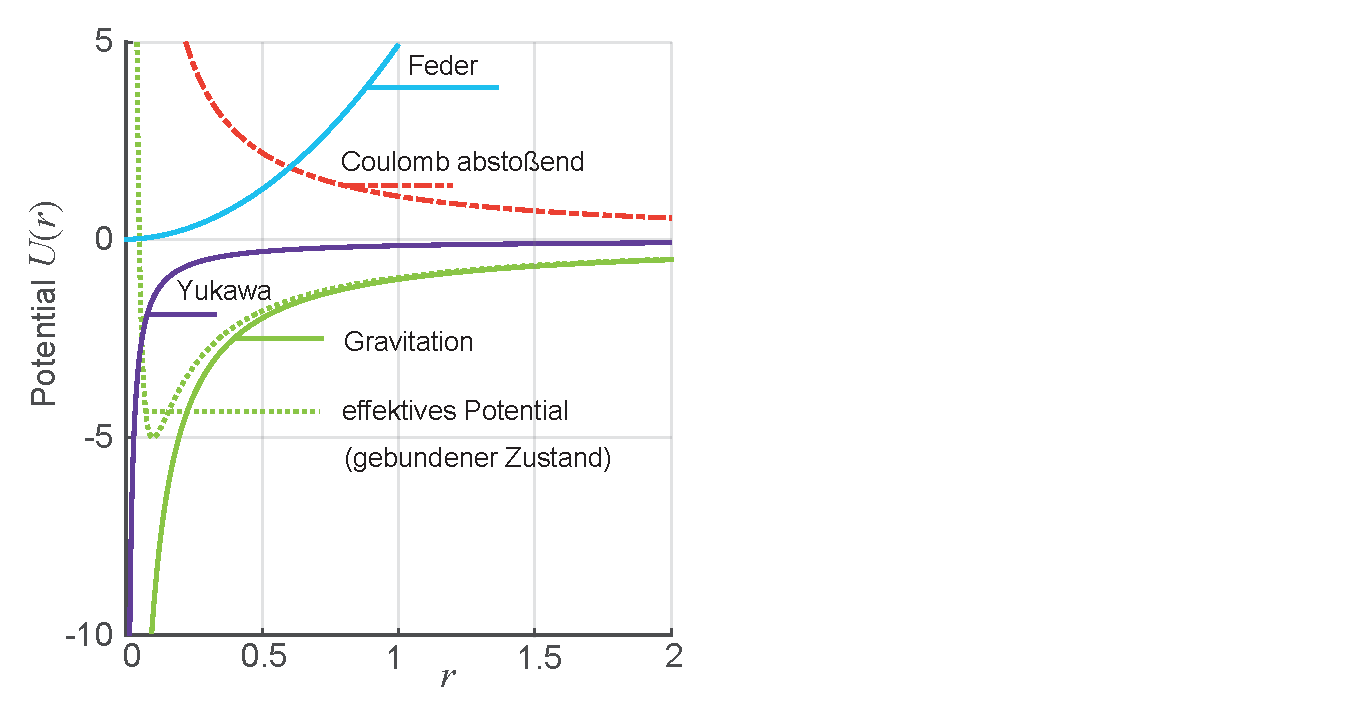
\includegraphics[width=\textwidth]{ZKF_Beispiele.pdf}
\caption[Beispiele f�r \pot{}e verschiedener Zentralkraftfelder.] {Beispiele f�r \pot{}e verschiedener Zentralkraftfelder: Newtonsche Gravitation, Coulomb-Kraft (sich absto�ende Ladungen), Kernkraft (aus Yukawa\indexp{Yukawa, Hideki}-\pot) und Federkraft. Ebenfalls gezeigt ist das effektive \pot{} $U_\text{eff}$ \eqref{eq:bew_Eff_Potential} f�r die Gravitation unter Ber�cksichtigung des Drehimpulses. F�r die anderen \pot{}e (Ausnahme: Coulomb-Potential bei sich absto�enden Ladungen) gibt es ebenfalls effektive \pot{}e und damit die M�glichkeit gebundener Zust�nde.}
\label{abb:bew_ZKF_Beispiele}
\end{figure}


\subparagraph{\textbf{Drehimpuls und Energieerhaltung, effektives \pot}}

Wir k�nnen uns das L�sen der Bewegungsgleichung \eqref{eq:bew_eff_EKP} vereinfachen, indem wir die Erhaltungss�tze ausnutzen. 
Daher wollen wir als erstes Erhaltungsgr��en identifizieren%
\footnote{H�ufig, besonders auch in der Himmelsmechanik,
werden Erhaltungsgr��en auch Bewegungsintegrale genannt,
da das Identifizieren einer Erhaltungsgr��e einer einmaligen
Integration der Bewegungsgleichung entspricht.}.

Der Drehimpulserhaltungssatz \eqref{eq:bew_Ges_Drehimpulserhaltung} kann f�r das allgemeine Zentralkraft\potsuf{} in ebenen Polarkoordinaten geschrieben werden als 
\begin{align}
  \left|\vec{L}\right| = m_\text{eff}\: \left|\vec{r} \times \dot{\vec{r}} \right| = L = \text{const} =   m_\text{eff}\: r^2 \dot{\varphi}\,. \label{eq:bew_Drehimp_polar}
\end{align}
Der Energieerhaltungssatz \eqref{eq:bew_Ges_Energieerhaltung} in diesen Koordinaten lautet:
\begin{align}
  E &= T + U = \text{const} = \frac{1}{2}  m_\text{eff}\: \dot{\vec{r}}^2 + U(r) =  \frac{1}{2}  m_\text{eff}\: \dot{r}^2 + \frac{L^2}{2  m_\text{eff}\: r^2} + U(r)\,, \label{eq:bew_Energie_polar}
\end{align}
womit wir durch
\begin{align}
	U_\text{eff}(r) &= U(r) + \frac{L^2}{2  m_\text{eff}\: r^2} \label{eq:bew_Eff_Potential}
\end{align}
das sogenannte \emph{effektive \pot}\index{Potential!effektives} definieren, in welchem sich (mathematisch gesehen) die effektive Masse $m_\text{eff}$ bewegt.
Mit diesen beiden Erhaltungss�tzen wollen wir das Zweik�rperproblem im Zentralkraftfeld l�sen.

\subparagraph{\textbf{Bahnkurven im Newtonschen Zentralkraftfeld  $U(r)= -\kappa/r$}}

Oft ist man gar nicht an der zeitlichen Entwicklung der Bewegung, sondern nur an der r�umlichen Form der Bahn interessiert.
Man kann daran \zb erkennen, ob die Bahn geschlossen, gebunden ($r$ bleibt endlich) oder ungebunden ($r$ divergiert) ist.
Wiederum unter Verwendung ebener Polarkoordinaten l�sst sich die Bahnkurve mit \eqref{eq:bew_Energie_polar} �ber
\begin{align}
	\frac{\mathrm{d}r}{\mathrm{d}\varphi} = \frac{\mathrm{d}r}{\mathrm{d}t} \frac{\mathrm{d}t}{\mathrm{d}\varphi} = \frac{\dot{r}}{\dot{\varphi}} = \frac{\sqrt{2 \lk E - U_\text{eff}(r) \rk/ m_\text{eff}\:}}{L/\lk m_\text{eff} r^2 \rk}
\end{align}
aus dem \pot{} $U_\text{eff}(r)$ berechnen.
Hierbei ergibt sich der Z�hler aus dem Energieerhaltungssatz, der Nenner aus dem Drehimpulserhaltungssatz.
Wir haben also aus den beiden Erhaltungss�tzen
eine Differentialgleichung f�r die Bahnform erhalten,
die man bei bekanntem effektiven \potz{} l�sen kann,
wodurch man die Bahnkurve
\begin{align}
\varphi(r) - \varphi_0 &=  L \int\limits_{r_0}^{r} \frac{\D r'}{r'^2 \sqrt{2  m_\text{eff}\: \lk  E - U_\text{eff}(r') \rk}} 
= L \int\limits_{r_0}^{r} \frac{\D r'}{r'^2 \sqrt{2  m_\text{eff}\: \lk E + \kappa/r' - L^2/(2  m_\text{eff}\,r'^2) \rk}}~, \label{eq:bew_Bahn_implizit1}
\end{align}
\bzw mit $r'=1/q'$
\begin{align}
\varphi(q) - \varphi_0 &= - L \int\limits_{q_0}^{q} \frac{\D q'}{\sqrt{2  m_\text{eff}\, E + 2  m_\text{eff}\,\kappa  q' - L^2\,  +-q'^2}} \label{eq:bew_Bahn_implizit2}
\end{align}
erh�lt.
Die in \eqref{eq:bew_Bahn_implizit1} und \eqref{eq:bew_Bahn_implizit2} auftretende Energie $E$ und der konstante Drehimpuls $L$ bilden zusammen mit den Anfangsbedingungen die Integrationskonstanten und legen damit die Form der Bahnkurve eindeutig fest. 
Die Bahn ist also durch das effektive \potz{} und die physikalischen Erhaltungsgr��en Energie $E$ und Drehimpuls $L$ bestimmt, welche man in zwei konstante, wie wir sehen werden geometrische Parameter �berf�hren kann.
Diese sind die (numerische) \glslink{exzentr}{\emph{Exzentrizit�t}} $\epsilon$ und der \emph{\gls{bahnpar}} $p$: 
\begin{align}
                \epsilon &= \sqrt{\frac{2 L^2 E}{ m_\text{eff}\: \kappa^2} + 1} ~~ ( \geq 0)\text{ und} \label{eq:bew_Bahn_Exzentrizitaet} 
\end{align}
\begin{align}
		p &= \frac{ L^2}{ m_\text{eff}\: \kappa}\,. 	\label{eq:bew_Bahn_Parameter} 
\end{align}
Mit diesen Parametern kann man \eqref{eq:bew_Bahn_implizit2} integrieren (siehe \cite{Gradshteyn1980}) und erh�lt die allgemeine Bahnkurve im Newtonschen Gravitations\potsuf{} 
\begin{align}
	  r(\varphi) = \frac{p}{1+\epsilon \cos{(\varphi - \varphi_0)}}\,. \label{eq:bew_Bahn_explizit}
\end{align}

Man kann nun abh�ngig vom Parameter $\epsilon$ drei F�lle unterscheiden:
\begin{itemize}
	\item \emph{Ellipsenbahnen f�r} $\epsilon < 1$

F�r $\epsilon < 1$ ergibt \eqref{eq:bew_Bahn_explizit} eine Ellipsenbahn (\figref{bew_Ellipse_Hyperbel}a).
Dies kann man zeigen, indem man mit den geometrischen Parametern der Ellipse $a$ (gro�e Halbachse) und $b=a \sqrt{1-\epsilon^2} $ (kleine Halbachse) und dem Bahnparameter $p= a (1-\epsilon^2)$ die Erf�llung der Ellipsengleichung zeigt.
Der Fall $\epsilon=0$ entspricht dem Spezialfall der Kreisbahn.

\begin{figure}
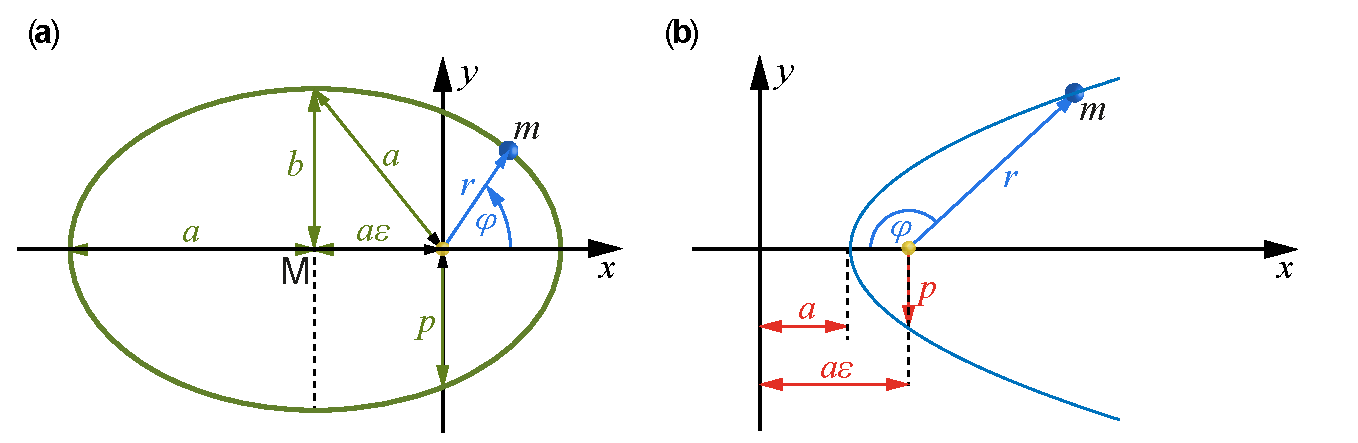
\includegraphics[width=\textwidth]{Ellipse_Hyperbel.pdf}
\caption[Geometrie von Ellipse und Hyperbel.] {Geometrie von \fa Ellipse und \fb Hyperbel.}
\label{abb:bew_Ellipse_Hyperbel}
\end{figure}

Im Newtonschen Gravitations\potsuf{} \eqref{eq:bew_Gravitationskraft} ist $\kappa > 0$, woraus wegen \eqref{eq:bew_Bahn_Exzentrizitaet} f�r $\epsilon < 1$ sofort $E <0$ folgt.
Bahnen k�nnen im $1/r$-\pot{} also nur dann gebunden sein, wenn $E < 0$ gilt.
Man sieht das auch an \eqref{eq:bew_Bahn_explizit}, wo wegen $\epsilon < 1$ der Nenner $ 1+ \epsilon\cos{\varphi}$ stets positiv und $r$ damit endlich ist.\\

\item \emph{Hyperbelbahnen f�r} $\epsilon > 1$

Der Fall $\epsilon > 1$ f�hrt wegen \eqref{eq:bew_Bahn_Exzentrizitaet} zwingend auf $E > 0$.
Gleichung \eqref{eq:bew_Bahn_explizit} beschreibt dann einen der beiden �ste einer Hyperbel (\figref{bew_Ellipse_Hyperbel}b).
Der Abstand $r$ wird unendlich, wenn $\:1 + \epsilon \cos{(\varphi -\varphi_0)}$ gegen Null strebt.
Die Bahn ist dann eingeschr�nkt auf
\begin{align}
	\left| \varphi \right| \: &\leq \varphi_\infty = \arccos \lk -\frac{1}{\epsilon} \rk \leq \frac{\pi}{2} \; , \nonumber \\
	r_\text{min} &= \frac{p}{1+\epsilon} \leq r \: \leq \infty\;.\label{eq:bew_hyp_asymptote}
\end{align}
Diese Art der Bewegung mit einem eingeschr�nkten Winkelbereich f�r $\varphi$ nennt man \emph{Streuung}\index{Streuung} (\figref{bew_Streuwinkel}).
Der Massepunkt kommt aus dem Unendlichen, wechselwirkt im \pot{} und l�uft anschlie�end unter einem \emph{Streuwinkel}\index{Streuwinkel} wieder ins Unendliche.
Wir werden im n�chsten Kapitel diese Streuprozesse genauer untersuchen.
Wir weisen hier explizit darauf hin, dass Hyperbelbahnen nicht nur durch anziehende \pot{}kr�fte wie die Newtonsche Gravitation entstehen k�nnen, sondern auch durch absto�ende \pot{}e wie sie durch gleichartige Ladungen hervorgerufen werden.
Man erkennt aus \eqref{eq:bew_Bahn_Exzentrizitaet}, dass die Exzentrizit�t $\epsilon$ der Bahn unabh�ngig vom Vorzeichen von $\kappa$ ist, der Bahnparameter $p$ wird bei $\kappa < 0$ jedoch negativ.
Da f�r den Abstand immer $r \geq 0$ gilt, muss der Nenner von \eqref{eq:bew_Bahn_explizit} insgesamt negativ werden, was nur f�r $\epsilon > 1$ und damit $ E > 0$ erf�llt werden kann.
F�r absto�ende Zentralkraft\potsuf{}e existieren damit keine gebundenen Bahnen. \\

\item \emph{Parabelbahnen f�r} $\epsilon = 1$

F�r $\epsilon = 1$ folgt aus \eqref{eq:bew_Bahn_explizit} der Spezialfall einer Parabelbahn.
Wir wollen diese hier nicht weiter behandeln, da man \zb in der Himmelsmechanik in der Regel Ellipsenbahnen bei gebundenen und Hyperbelbahnen bei ungebundenen Himmelsk�rpern beobachtet. 
\end{itemize}
Wir haben hier nur einen kurzen Abriss der Physik der Bewegung im Zentralkraftfeld gegeben, der uns aber erlaubt, eine Reihe von Problemen und �bungen zu l�sen (siehe \zb \probref{bew_SwingBy}).
Im Kapitel Himmelsmechanik (Band II, Kapitel 3) werden wir
die Bewegungen auch in ihrer Zeitabh�ngigkeit berechnen
und zudem Abweichungen von diesen einfachen Bahnen detailliert
untersuchen.
Wir werden dort auch eine leicht andere (\zt durch historische Konventionen bedingte) Notation verwenden und mit sogenannten spezifischen, \dh auf die Masse des bewegten K�rpers bezogenen Gr��en rechnen.

\subsubsection{Sto�- und Streuprozesse}\index{Sto�} \index{Streuung|textbf} \label{kap:bew_stoss}

\subparagraph{\textbf{Bezugssystem bei Streuung}} \index{Schwerpunktsystem}

Wir wollen uns nun den Sto�- und Streuprozessen\footnote{Sto� und Streuung werden h�ufig synonym gebraucht.
Unter Streuung verstehen wir die �nderung der Bewegung eines Teilchens/K�rpers durch Wechselwirkung mit einem anderen Teilchen/K�rper.
Sto� bezeichnet hingegen den speziellen Fall, dass sich die beiden Teilchen/K�rper bei dieser Wechselwirkung ber�hren, was nat�rlich bei St��en von Massepunkten nur ein theoretisches Konzept (wie der Massepunkt selbst), bei ausgedehnten K�rpern aber sehr wohl von Bedeutung ist.} zweier Massepunkte zuwenden.
Wir haben gesehen, dass bei der Streuung die einfallenden Teilchen um den sogenannten Streuwinkel\index{Streuwinkel} $\vartheta$ abgelenkt werden.
Wir werden jetzt zeigen, dass sich $\vartheta$ aus dem Wechselwirkungs\potsuf{} \index{Potential!Wechselwirkungspotential} berechnen l�sst.
Daher lassen sich aus der experimentellen Bestimmung von Streuwinkeln und des damit zusammenh�ngenden (noch zu definierenden)  Wirkungsquerschnitts R�ckschl�sse �ber die Art und Gr��e der Wechselwirkung ziehen.
Bei der Behandlung der Streuprozesse wollen wir zwei Bezugssysteme verwenden:

\begin{enumerate}
	\item das Laborsystem $\vec{\Sigma}_\text{L}$, in dem das Experiment beobachtet und beschrieben wird und die Koordinaten ungestrichen (\zb $x$) gekennzeichnet sind, und 
	\item das Schwerpunktsystem $\vec{\Sigma}_\text{S}$, in welchem der Schwerpunkt des Systems im Ursprung ruht und die Koordinaten gestrichen (\zb $x'$) sind. 
\end{enumerate}

\subparagraph{\textbf{Elastische Streuung zwischen zwei Teilchen}}\index{Streuung!elastische}

\begin{figure}
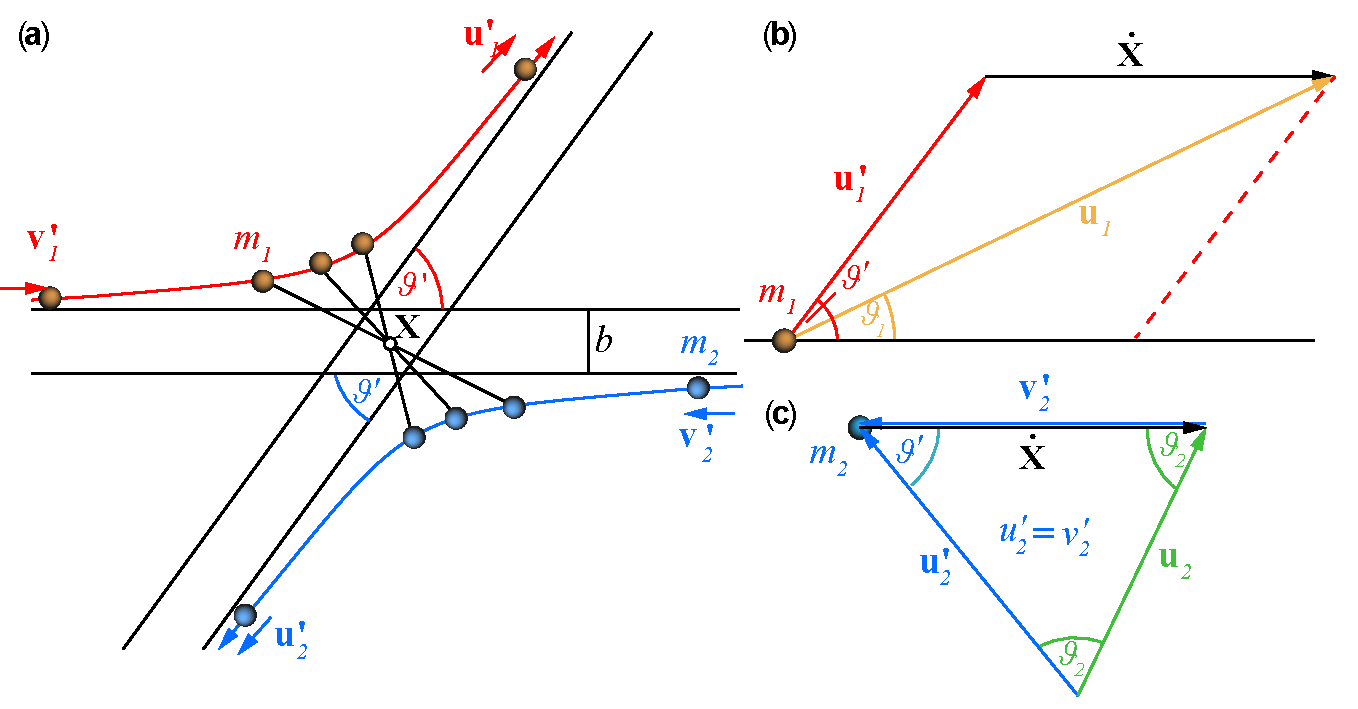
\includegraphics[width=\textwidth]{Streuwinkel.pdf}
\caption[Streuwinkel im Schwerpunktsystem und im Laborsystem.] {\fa Streuwinkel $\vartheta'$ im Schwerpunktsystem $\vec{\Sigma}_\text{S}$ f�r zwei gleiche Massen $m_1 = m_2$. Dargestellt sind auch die Asymptoten ins Unendliche und der asymptotische Abstand $b$, der Sto�parameter genannt wird. \fb Beziehung zwischen den Streuwinkeln $\vartheta'$ in $\vec{\Sigma}_\text{S}$ und $\vartheta_1$ des bewegten Teilchens $m_2$ im Laborsystem $\vec{\Sigma}_\text{L}$. Die Masse $m_2$ ruht vor dem Sto� in $\vec{\Sigma}_\text{L}$. \fc Beziehung zwischen dem Streuwinkel $\vartheta'$ f�r die bewegte Masse $m_1$ in $\vec{\Sigma}_\text{S}$ und dem Winkel $\vartheta_2$ des anfangs ruhenden Teilchens $m_2$ im Laborsystem $\vec{\Sigma}_\text{L}$ (nach \cite{Bartelmann2015}).}
\label{abb:bew_Streuwinkel}
\end{figure}

Wir wollen uns auf elastische Wechselwirkungen beschr�nken, die noch dazu im Unendlichen verschwinden.
Dabei bleibt die mechanische Energie, \dh die Summe aus kinetischer und potenzieller Energie, erhalten.
Neben dem Energieerhaltungssatz gilt auch der Impulserhaltungssatz, wobei wir annehmen, dass sich die Massen der wechselwirkenden Teilchen nicht �ndern.
Wir betrachten  die Massen $m_1$ und $m_2$ mit den Geschwindigkeiten $\vec{v}_1$ und $\vec{v}_2$ vor dem Sto� und $\vec{u}_1$ und $\vec{u}_2$ nach dem Sto�.
Dann gelten im Unendlichen (wo das \pot{} verschwindet) 
\begin{align}
	\text{Impulserhaltung:} \qquad &m_1 \,\vec{v}_1 + m_2\, \vec{v}_2 = m_1 \,\vec{u}_1 + m_2 \,\vec{u}_2   \label{eq:bew_Streuung1} \\ 
	\text{und Energieerhaltung:} \qquad &\frac{m_1}{2}\, \vec{v}_1^2 + \frac{m_2}{2} \, \vec{v}_2^2 = \frac{m_1}{2} \,\vec{u}_1^2 +\frac{m_2}{2}\, \vec{u}_2^2\,. \label{eq:bew_Streuung2}
\end{align}
Die entsprechenden Erhaltungss�tze lauten im Schwerpunktsystem folglich
\begin{align}
	m_1 \,\vec{v'}_1 + m_2 \,\vec{v'}_2 &= m_1\,\vec{u'}_1 + m_2 \,\vec{u'}_2 = 0 \qquad \text{und} \label{eq:bew_Streuung1a} \\ 
	\frac{m_1}{2} \,\vec{v'}_1^2 + \frac{m_2}{2} \,\vec{v'}_2^2 &= \frac{m_1}{2} \,\vec{u'}_1^2 +\frac{m_2}{2} \,\vec{u'}_2^2\,. \label{eq:bew_Streuung2a}
\end{align}
Damit ergibt sich der Streuwinkel $\vartheta'$ als Winkel zwischen einfallender Bahn und auslaufender Bahn im Schwerpunktsystem (siehe \figref{bew_Streuwinkel}) wegen $m_1 \,\vec{v'}_1 = - m_2 \,\vec{v'}_2$ sofort zu
\begin{align}
	\cos\vartheta' = \frac{\vec{v'}_1 \cdot \vec{u'}_1}{\left|\vec{v'}_1\right| \left|\vec{u'}_1\right|} = \frac{\vec{v'}_2 \cdot \vec{u'}_2}{\left|\vec{v'}_2\right| \left|\vec{u'}_2\right|}\,. \label{eq:bew_Streuung3}
\end{align} 
Da der Gesamtimpuls in $\vec{\Sigma}_\text{S}$ verschwindet, ist der Streuwinkel  $\vartheta'$ f�r beide Teilchen gleich gro�.
Wir sind aber mehr an dem Streuwinkel $\vartheta$ im Laborsystem $\vec{\Sigma}_\text{L}$ interessiert, da nur dieser direkt gemessen werden kann. Er h�ngt vom Wechselwirkungs\potsuf{} zwischen den Teilchen ab.
Die Frage ist also, wie man $\vartheta'$ und $\vartheta$ ineinander umrechnen kann.
Wir wollen hier den Spezialfall betrachten, dass eine Masse (\zb $m_2$) vor dem Sto� bzw. der Streuung im Laborsystem ruht, also $v_2$ = 0.
Dann ist die Bewegung des Schwerpunktes im Laborsystem gegeben durch
\begin{align}
	\dot{\vec{e}}_x(t) = \frac{m_1 \,\vec{v}_1(t)}{m_1 + m_2} = \frac{m_1}{M} \,\vec{v}_1\,.\label{eq:bew_Streuung4}
\end{align}
Diese Gleichung besagt nichts anderes, als dass der Geschwindigkeitsvektor $\vec{v}_1$ des einfallenden Teilchens logischerweise parallel zum Geschwindigkeitsvektor des Schwerpunktes liegt.
Beim �bergang in das Schwerpunktsystem gelten folgende Beziehungen: 
\begin{align}
		\vec{v}_1' = \vec{v}_1 - \dot{\vec{e}}_x(t) &= \vec{v}_1 - \frac{m_1}{M}\,\vec{v}_1 = \frac{m_2}{M}\,\vec{v}_1\,,\nonumber \\
                \text{und}\qquad\vec{u}_1' = \vec{u}_1 - \dot{\vec{e}}_x(t) &= \vec{u}_1 - \frac{m_1 }{M}\,\vec{v}_1\,.\label{eq:bew_Streuung5}
\end{align}
Wenn man diese Vektorbeziehung %\eqref{eq:bew_Streuung5}
graphisch in der von $\dot{\vec{X}}$ und $\vec{v}_1'$ aufgespannten Ebene darstellt (\figref{bew_Streuwinkel}b), sieht man, dass 
\begin{align}
        u_1 ~ \sin\vartheta_1 &= u_1' ~ \sin\vartheta'\text{\qquad und}\nonumber \\
	u_1 ~ \cos\vartheta_1 &= u_1' ~ \cos\vartheta' + \dot{\vec{X}} = u_1' ~ \cos\vartheta' + \frac{m_1}{M} v_1 \label{eq:bew_Streuung6}
\end{align}
gelten und daraus sofort
\begin{align}
	\tan\vartheta_1  &= \frac{\sin\vartheta_1}{\cos\vartheta_1} = \frac{\sin\vartheta'}{\cos\vartheta' + \frac{m_1}{m_2}} \label{eq:bew_Streuung7}
\end{align}
folgt.
Nach �hnlicher geometrischer Betrachtung (\figref{bew_Streuwinkel}c) ergibt sich f�r den Streuwinkel $\vartheta_2$ des urspr�nglich ruhenden Teilchens 
\begin{align}
	\vartheta_2   &= \frac{\pi -\vartheta'}{2}\,. \label{eq:bew_Streuung8}
\end{align}
Dies sind wichtige Zwischenergebnisse (\figref{bew_StreuwinkelUmrechnung}),
die insbesondere zeigen, dass die Streuwinkel in beiden Systemen gleich gro� sind,
wenn die ruhende Masse als sehr viel gr��er als die bewegte angenommen wird ($m_2 \gg m_1$).
Wir geben jetzt noch die Beziehung f�r den Energie�bertrag beim elastischen Sto� an.
Im System $\vec{\Sigma}_\text{S}$ gilt logischerweise $\vec{u}_i'^2 = \vec{v}_i'^2$.
Im System $\vec{\Sigma}_\text{L}$ kommt es aber zu einem Energie�bertrag zwischen den beiden Teilchen.
Wir k�nnen diesen Energie�bertrag f�r den Fall $\vec{v}_2 = 0$
ausgehend von \eqref{eq:bew_Streuung2} und \eqref{eq:bew_Streuung2a}
sowie unter Verwendung von \eqref{eq:bew_Streuung4} und \eqref{eq:bew_Streuung6}
wie folgt angeben (\probref{bew_SwingBy}):
\begin{align}
	\frac{\Delta T}{T_1^{\text{\,(init)}}} = \frac{{T_1^{\text{\,(final)}}} - T_1^{\text{\,(init)}}} {T_1^{\text{\,(init)}}} &= 2\: \frac{m_1}{M} \lk 1 - \frac{m_1}{M} \rk  \lk \cos\vartheta' -1 \rk\,, \label{eq:bew_Streuung9}
\end{align}
wobei $\cos\vartheta'$ �ber die Beziehung \eqref{eq:bew_Streuung7} mithilfe des gemessenen Streuwinkels $\vartheta$ im Laborsystem ausgedr�ckt werden kann und $T^{\text{\,(init)}}$  \bzw $T^{\text{\,(final)}}$ f�r die kinetische Energie im Ausgangszustand (init) \bzw Endzustand (final) der Streuung stehen.
Die Abh�ngigkeit des Energie�bertrags vom Streuwinkel ist in \figref{bew_EnergieUebertrag} dargestellt.
Eine sch�ne Anwendung erf�hrt dies in der Raumfahrt: Beim sogenannten Swing-By-Man�ver wird eine Raumsonde im Vorbeiflug an einem Planeten in dessen Gravitationsfeld gestreut.
Bei diesem Man�ver ist zwar im Schwerpunktsystem (von Sonde und Planet) die Geschwindigkeit der Raumsonde nach dem Vorbeiflug genauso gro� wie vorher, jedoch nicht im Bezugssystem der Sonne, wodurch Raumsonden relativ zur Sonne beschleunigt werden und so, wie \zb die  Voyager-Missionen, ins �u�ere Sonnensystem vordringen k�nnen.
Wir werden das ausf�hrlich in der Astrodynamik (Band II, Kapitel 4) untersuchen, wollen hier aber schon auf \probref{bew_SwingBy} verweisen. 
F�r eine umfassende Betrachtung des Streuproblems fehlt noch die Berechnung des Streuwinkels als Funktion des \pot{}s.
Diese wollen wir jetzt angehen.

\begin{figure}
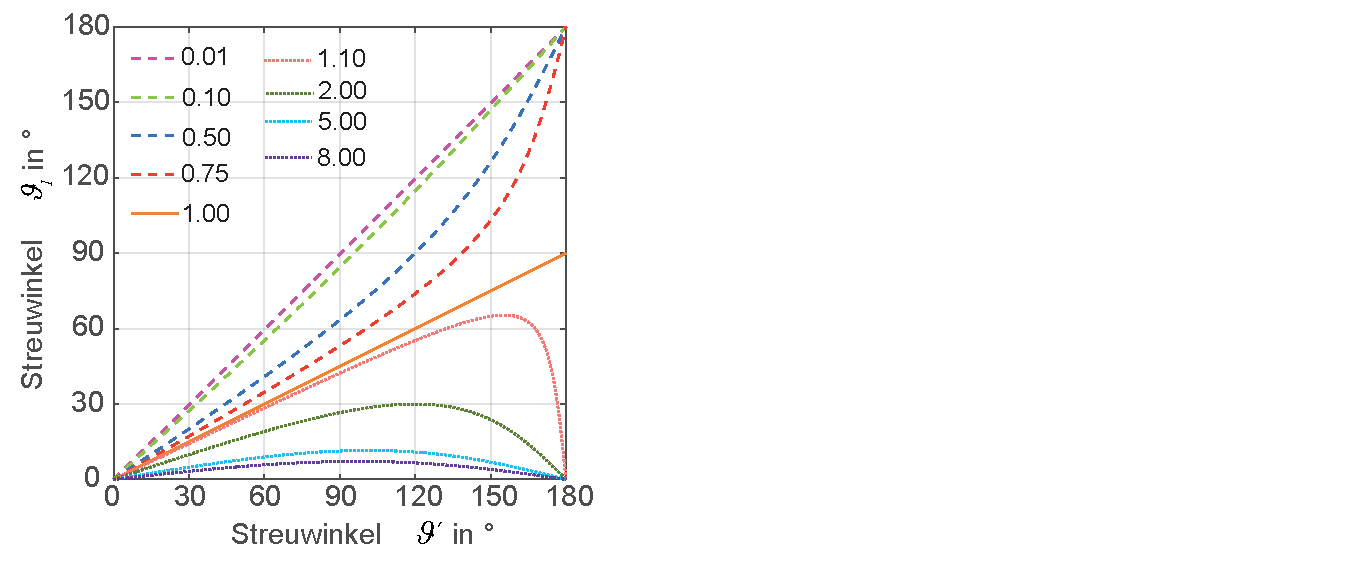
\includegraphics[width=\textwidth]{StreuwinkelUmrechnung.pdf}
\caption[Umrechnung von Streuwinkeln.]{Umrechnung des Streuwinkels $\vartheta'$ aus dem Schwerpunktsystem in den Streuwinkel $\vartheta_1$ im Laborsystem als Funktion verschiedener Massenverh�ltnisse $m_1/m_2$. Die Masse $m_2$ wird vor dem Sto� als ruhend angenommen. Vergleiche Gl. \eqref{eq:bew_Streuung7}.}
\label{abb:bew_StreuwinkelUmrechnung}
\end{figure}

\begin{figure}
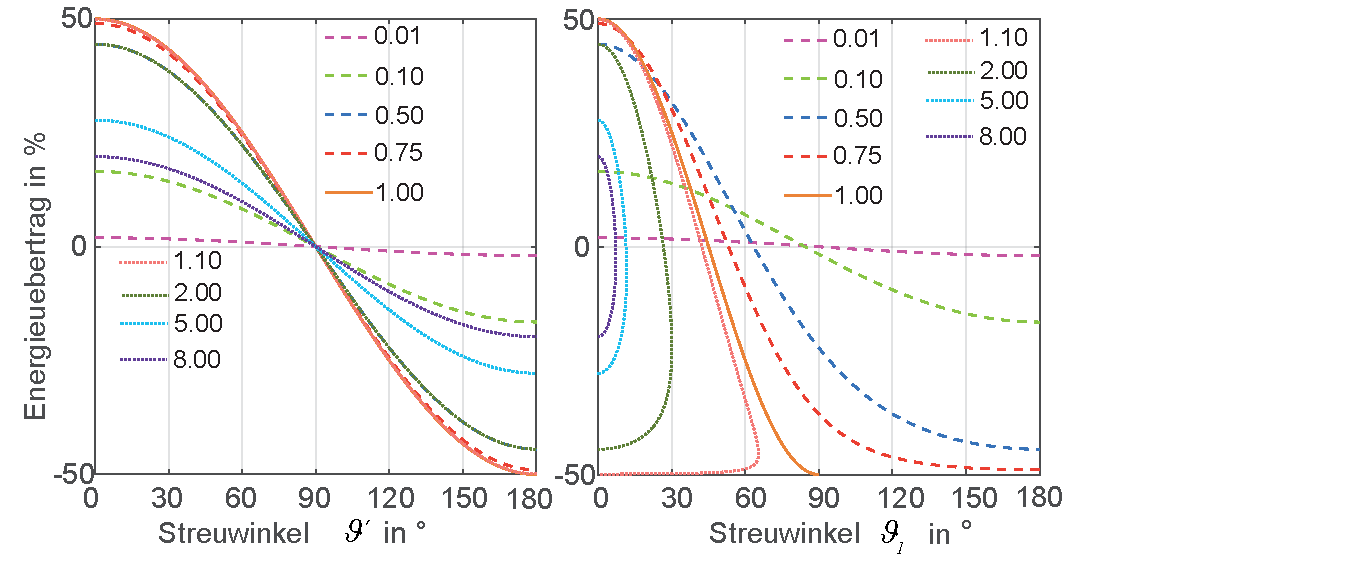
\includegraphics[width=\textwidth]{EnergieUebertrag.pdf}
\caption[Energie�bertrag beim elastischen Sto�.]{Energie�bertrag beim elastischen Sto� als Funktion verschiedener Massenverh�ltnisse $m_1/m_2$ als Funktion der Streuwinkels $\vartheta$ \bzw $\vartheta'$. Die Masse $m_2$ wird vor dem Sto� als ruhend angenommen. Vergleiche Gl. \eqref{eq:bew_Streuung9}.}
\label{abb:bew_EnergieUebertrag}
\end{figure}

\subparagraph{\textbf{Streuwinkel und Wirkungsquerschnitte bei Streuung im Zentralkraftfeld}}

Bisher haben wir f�r die \pot{}e nur angenommen, dass sie im Unendlichen verschwinden und haben daraus ein paar grunds�tzliche Eigenschaften der Streuung hergeleitet.
Wir wollen nun bestimmte Formen des Wechselwirkungs\potsuf{}s sowie der Energie und des (Dreh-)Impulses des einfallenden Teilchens annehmen.
Als Messgr��e bei der Streuung ermittelt man im Allgemeinen, wie viele Teilchen eines einfallenden Stromes von Teilchen durch ein Streuzentrum unter einem bestimmten Streuwinkel abgelenkt \bzw gestreut werden.
Wir nehmen wieder an, dass das Teilchen aus dem Unendlichen kommt und in das Wechselwirkungs\potsuf{} $U$ des Teilchens mit Masse $m_2$ gelangt.
Wir wollen ferner f�r das \pot{} ein Zentralkraft\potsuf{} annehmen, das also nur vom relativen Abstand der beiden Teilchen abh�ngt.
Wir k�nnen das System dann durch das �quivalente Einteilchenproblem (siehe \kap{bew_ZKP_EEKP}) mit der effektiven Masse $m_\text{eff}$ im Schwerpunktsystem $\vec{\Sigma}_\text{S}$ beschreiben.
Dann gilt f�r die Erhaltungsgr��e Energie 
\begin{align}
	E = \frac{m_\text{eff}}{2}\: v_\infty^2\,, \label{eq:bew_Streuung10}
\end{align}
mit $v_\infty$ als Relativgeschwindigkeit im Unendlichen.
F�r den ebenfalls konstanten Betrag des Drehimpulses gilt
\begin{align}
	L = b\:m_\text{eff}\:v_\infty \,, \label{eq:bew_Streuung11}
\end{align}
wobei $b' = b$ wieder der bereits eingef�hrte Sto�parameter\index{Sto�parameter} (\figref{bew_Streuwinkel}) ist, der in den beiden Systemen �bereinstimmt.
Wegen \eqref{eq:bew_Streuung8} ist $E > 0$ und die Teilchenbahn eine Hyperbel.
Der Streuwinkel $\vartheta'$ kann nach \eqref{eq:bew_Bahn_implizit1} mit $ r \rightarrow \infty $ berechnet werden zu
\begin{align}
	\vartheta' = \pi - \Delta \varphi = \pi - 2 b \int\limits_{r_\text{min}}^\infty \frac{\D r'}{r'^2 \sqrt{1-\frac{b^2}{r'^2}-\frac{U(r')}{E}}}\,. \label{eq:bew_Streuung12}
\end{align}
Hierbei haben wir die Ausdr�cke f�r die Energie \eqref{eq:bew_Streuung10} und den Drehimpuls \eqref{eq:bew_Streuung11} benutzt.
Wenn man also das Wechselwirkungs\potsuf{} $U(r)$ und die Energie $E$ eines einfallenden Streuteilchens kennt, h�ngt der Streuwinkel nur noch vom Sto�parameter $b$ ab.
Andererseits kann man R�ckschl�sse �ber das \pot{} erlangen, indem man $\vartheta$ als Funktion von $b$ misst.
Genau das war die Idee des ber�hmten Streuexperimentes von Rutherford.\footnote{Sir Ernest Rutherford\indexp{Rutherford, Sir Ernest} (1871--1937) war ein britisch-neuseel�ndischer Physiker. Als einer der bedeutendsten Experimentalphysiker erhielt er 1908 den Nobelpreis f�r Chemie (sic!) und sein wichtigster Beitrag zur Atomphysik ist das nach ihm benannte Atommodell, welches er 1911 aus seinen Streuversuchen von $\alpha$-Teilchen an Goldfolie herleitete.}
In diesem Experiment war das Wechselwirkungs\potsuf{} ein \gls{coulpot}
$U(r) = -\alpha/r$ und man erh�lt durch Einsetzen von
$\Delta \varphi_\infty = 2 \arccos(-1/\epsilon)$ und $\epsilon$ aus
\eqref{eq:bew_Bahn_Parameter} in \eqref{eq:bew_Streuung12}
sowie Ausdr�cken des Drehimpulses mithilfe des Sto�parameters $b$
verm�ge \eqref{eq:bew_Streuung11} die Abh�ngigkeit des Streuwinkels von der Energie und dem Streuparameter:
\begin{align}
	\sin^2\lk \frac{\vartheta'}{2} \rk & \:=\: \frac{1}{1 + \frac{4 E^2 b^2}{\alpha^2}}\,. \label{eq:bew_Streuung13}
\end{align}
Oft wird auch der Streuparameter als Funktion des Streuwinkels angegeben:
\begin{align}
	b^2 & \:=\: \lk \frac{1}{\sin^2\lk \frac{\vartheta'}{2} \rk } -1 \rk \frac{\alpha^2}{4 E^2}\,. \label{eq:bew_Streuung13a}
\end{align}
\begin{figure}
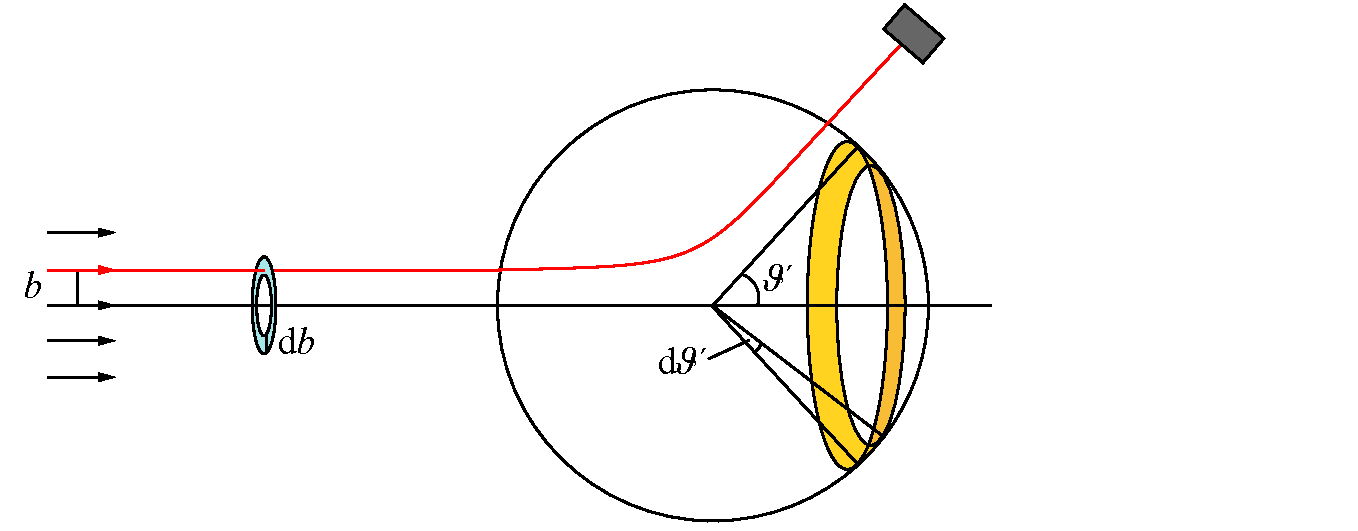
\includegraphics[width=\textwidth]{Wirkungsquerschnitt.pdf}
\caption[Geometrie der Streuung im Zentralkraftfeld und Wirkungsquerschnitt.]{Geometrie einer Streuung im Zentralkraftfeld und Wirkungsquerschnitt.}
\label{abb:bew_Wirkungsquerschnitt}
\end{figure}

Wir betrachten nun einen homogenen, konstanten Teilchenstrahl mit Teilchenstromdichte $I = N/(\Delta t \Delta A)$ in einem Zeitintervall $\Delta t$ und pro Fl�che $\Delta A$ (\figref{bew_Wirkungsquerschnitt}). 
Als Messgr��e im Streuexperiment wird die am Detektor pro Zeitintervall $\Delta t$ gemessene Anzahl von Streuteilchen $n(\vartheta')$ definiert.
Diese ist proportional zum Teilchenstrom $I$ und auch zur Detektorfl�che $\D\Omega$%
\footnote{Diese kann auch als Raumwinkelelement aufgefasst werden.}.
Der entsprechende Proportionalit�tsfaktor wird als differentieller Wirkungsquerschnitt\index{Wirkungsquerschnitt!differentieller} bezeichnet und folgenderma�en geschrieben:
\begin{align}
	\frac{\D \sigma'}{\D \Omega}  \:=\: \frac{n(\vartheta')}{I \Delta t \D \Omega}\,. \label{eq:bew_Streuung14}
\end{align}
Der totale Wirkungsquerschnitt\index{Wirkungsquerschnitt!totaler} ergibt sich dann als komplettes Raumwinkelintegral (bei Annahme einer Zylindersymmetrie) zu
\begin{align}
	\sigma' \:= \int \frac{\D \sigma'}{\D \Omega} \D \Omega = 2 \pi \int\nolimits_{0}^{\pi} \sin\vartheta' \D \vartheta' \frac{\D \sigma'}{\D \Omega}\,. \label{eq:bew_Streuung15}
\end{align}
Der totale Wirkungsquerschnitt ist quasi die \textit{effektive} Fl�che, an welcher der einfallende Teilchenstrom gestreut wird.
Man kann sowohl den differentiellen als auch den totalen Wirkungsquerschnitt in Beziehung zum Sto�parameter $b$ setzen.
Wir betrachten wieder \figref{bew_Wirkungsquerschnitt} und speziell den Kreisring mit der Fl�che $2 \pi b \D b$ des einfallenden Teilchenstromes (im Sto�parameterbereich $\left[b, b +\D b\right]$), der in den Raumwinkelbereich $\left[\vartheta', \vartheta' +\D \vartheta'\right]$ gestreut wird.
Wegen Teilchenerhaltung gilt\footnote{Man mache sich klar, dass die Absolutbetr�ge notwendig sind, da $\D b$ und $\D \vartheta'$ unterschiedliche Vor\-zei\-chen haben k�nnen.}
	\[I \lk 2 \pi b \left|\D b\right| \rk = I \lk 2 \pi \sin \vartheta' \frac{\D \sigma}{\D \Omega} \left| \D \vartheta' \right| \rk\,.
\]
Der differentielle Wirkungsquerschnitt h�ngt demnach mit dem Sto�parameter und dem Streuwinkel $\vartheta'$ wie folgt zusammen, wobei $b(\vartheta')$ f�r ein bestimmtes \pot{} aus \eqref{eq:bew_Streuung12} berechnet werden kann:
\begin{align}
	\frac{\D \sigma'}{\D \Omega}  =  \frac{b(\vartheta')}{\sin\vartheta'} \left| \frac{\D b(\vartheta')}{\D\vartheta'} \right| = \frac{1}{2 \sin\vartheta'} \left| \frac{\D b^2(\vartheta')}{\D\vartheta'} \right|\,. \label{eq:bew_Streuung16}
\end{align}
Die Messungen von Streuexperimenten liegen aber als Gr��en des Laborsystems $\vec{\Sigma}_\text{L}$ vor,
in denen das Streuzentrum ($m_2$) und der Detektor zumeist fest sind.
Daher
unterscheiden sich die differentiellen Streuquerschnitte in beiden Systemen und m�ssen mit der Beziehung \eqref{eq:bew_Streuung7} f�r die Streuwinkel umgerechnet werden.
Man erh�lt dann 
\begin{align}
	\frac{\D \sigma}{\D \Omega} = \frac{\D \sigma'}{\D \Omega} \left| \frac{\D \cos\vartheta'}{\D \cos\vartheta} \right| \,, \label{eq:bew_Streuung17}
\end{align}
worin die ungestrichenen Gr��en wie gehabt die Gr��en im Laborsystem darstellen.
Wir wollen zum Abschluss im folgenden Beispiel noch die Wirkungsquerschnitte f�r das Coulomb-Potential  berechnen, die der Form nach nat�rlich auch denen des Newtonschen Gravitations\potsuf{}s entsprechen.

%BEISPIEL 1 %%%%%%%%%%%%%%%%%%%%%%%%%%%%%%%%%%%%%%%%%%%%%%%%%%%%%%%%%%%%%%%%%%%%%%%%%%%%%%%%%%
\begin{example}{Wirkungsquerschnitte f�r Streuung in Zentralkraftfeldern (Coulomb-Potential)}
Mit $U(r) = -\alpha/r$ kann man zun�chst $b^2(\vartheta')$ nach \eqref{eq:bew_Streuung13} berechnen und davon die Ableitung bilden:
	\[ \left| \frac{\D b^2(\vartheta')}{\D\vartheta'} \right| = \frac{\alpha^2}{4 E^2} \frac{\cos\frac{\vartheta'}{2}}{\sin^3\frac{\vartheta'}{2}} = \frac{\alpha^2}{8 E^2} \frac{\sin\vartheta'}{\sin^4\frac{\vartheta'}{2}}\,.
\] 
Hierin ist $E$ die Energie des Teilchens.
Daraus folgt der differentielle Rutherford-Wirkungsquerschnitt\index{Wirkungsquerschnitt!Rutherford-} im Schwerpunktsystem
\begin{align}
	\frac{\D \sigma'}{\D \Omega}  = \lk \frac{\alpha}{4 E} \rk^2 \frac{1}{\sin^4\lk\vartheta'/2\rk} \,. 	\label{eq:bew_Streuung18}
\end{align}
Dies ist die  ber�hmte Streuformel von Rutherford\index{Streuformel!Rutherford-}. Der totale Wirkungsquerschnitt f�r das $U(r) = \alpha/r$-\pot{} ergibt sich durch Integration �ber $\vartheta'$ zu
\begin{align}
	\sigma' = 2 \pi \lk \frac{\alpha}{4 E} \rk^2 \int\limits_0^\pi \frac{\D \vartheta' \,\sin\vartheta'}{\sin^4\lk\vartheta'/2\rk} = \infty \,. 	\label{eq:bew_Streuung19}
\end{align}
und ist unendlich gro�, was schnell klar wird, da das \pot{} auch in beliebig gro�er Entfernung noch Teilchen streut.
Dies erkennt man auch daran, dass der differentielle Wirkungsquerschnitt f�r $\vartheta'=0$ divergiert.
In der Realit�t gibt es nat�rlich keine punktf�rmigen Streuzentren.
Entweder haben die Zentren eine Ausdehnung oder sie werden wie beim Atom teilweise abgeschirmt.
\label{bsp:SigmaCoulomb}
\end{example}
%BEISPIEL %%%%%%%%%%%%%%%%%%%%%%%%%%%%%%%%%%%%%%%%%%%%%%%%%%%%%%%%%%%%%%%%%%%%%%%%%%%%%%%%%%


\subsubsection{$N$-K�rper-Systeme}\index{Mehrk�rperproblem} \index{Streuung} \label{kap:bew_n_body}

Im Kapitel Himmelsmechanik (Band II, Kapitel 3) werden wir
viele F�lle kennenlernen, die nicht mehr als Zweik�rperproblem
modelliert werden k�nnen.
Das Mehrk�rper- oder $N$-K�rperproblem ist f�r $N>2$ nicht in analytischer Form l�sbar, man kann es aber mit st�rungstheoretischen Ans�tzen angehen.
Dabei betrachtet man das Problem zun�chst als Zweik�rpersystem und bezieht dann die Einfl�sse der weiteren K�rper \bzw Massen als St�rungen mit ein.
Ist das Zweik�rperproblem beispielsweise das Sonne-Erde-System, so lassen sich die Einfl�sse der anderen Planeten auf die Erdbahn auf diese Weise absch�tzen.
Allerdings ist dieser Ansatz nur dann erfolgversprechend,
wenn die St�rungen gering sind.
In anderen F�llen muss man auf numerische Verfahren zur�ckgreifen (siehe \zb \cite{Dehnen2011}).
Wir werden in der Himmelsmechanik sowohl st�rungstheoretische als auch numerische Methoden f�r die Berechnung der Planetenbewegung anwenden. 
Zus�tzlich wollen wir uns hier kurz mit einem Spezialfall
des Dreik�rperproblems besch�ftigen,
welcher trotz seiner begrenzenden Annahmen von gro�er Bedeutung f�r
das Verst�ndnis der Mechanik des Sonnensystems und �hnlicher Probleme ist.

\subsubsection{Das eingeschr�nkte Drei-K�rper-System}\index{Dreik�rperproblem} \index{Dreik�rperproblem!reduziertes} \index{Dreik�rperproblem!eingeschr�nktes}\label{kap:bew_3_body}

\begin{figure}%
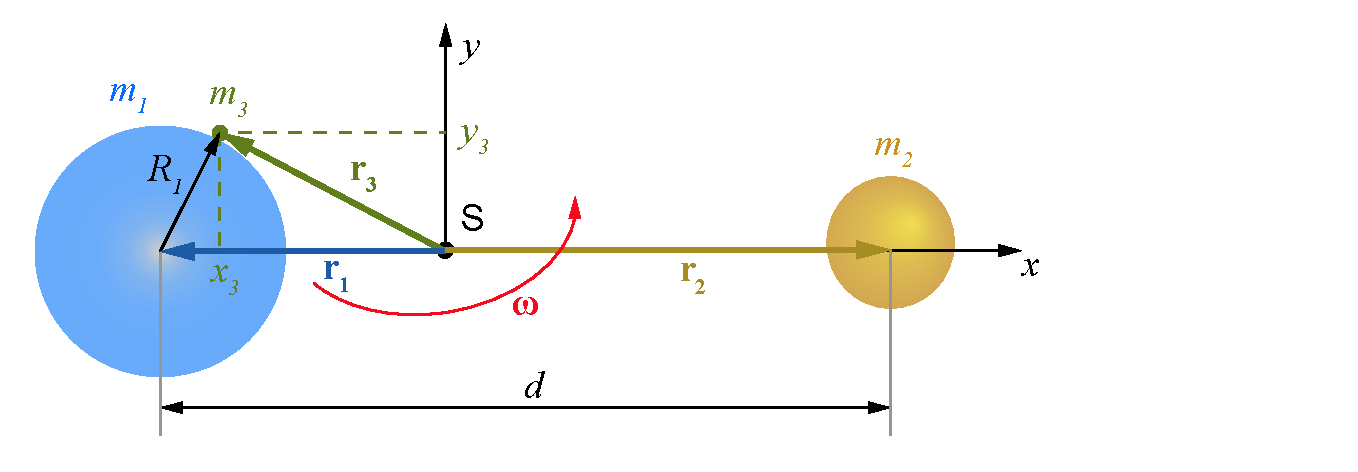
\includegraphics[width=\textwidth]{Geometrie3KP.pdf}%
\caption[Geometrie des reduzierten Dreik�rperproblems.]{Geometrie des reduzierten Dreik�rperproblems.}%
\label{abb:bew_3KoerperP01}%
\end{figure}

Wir betrachten in \figref{bew_3KoerperP01} die Geometrie des sogenannten eingeschr�nkten  Dreik�rperproblems.
Es soll gelten $m_3 \ll m_1,m_2$.
Die Masse $m_1$ k�nnte \zb die Sonnenmasse $m_{\astrosun}$ und die Masse $m_2$ gleich der Erdmasse $m_{\earth}$ sein.
Die kleine Masse $m_3$ w�re dann \zb ein Satellit oder ein Asteroid.
Wir definieren zur Vereinfachung
		\begin{align}
				p = \frac{m_1}{m_1+m_2}<1 \qquad \text{und} \qquad 1-p= \frac{m_2}{m_1+m_2}<1 \,. \label{eq:bew_red3KP01}
		\end{align}
Damit haben im mitrotierenden Schwerpunktsystem $\vec{\Sigma}'$ die Massen $m_1$ und $m_2$ die Koordinaten\footnote{Der Einfachheit halber lassen wir in \kap{bew_3_body} 
%und Kap. \label{kap:gezeiten}
 die Striche an den Koordinatengr��en im mitbewegten \KOS{} weg, da wir ausschlie�lich in diesen System bleiben.}:
		\begin{align}
				\vec{r}_1 = 
				\begin{pmatrix}
				(p-1)d  \\
				0 \\
				0 
				\end{pmatrix}
~~~~				\text{und} \quad
				r_2 = 
				\begin{pmatrix}
				p\,d  \\
				0 \\
				0 
				\end{pmatrix}
				\,.
				\label{eq:bew_red3KP02}
		\end{align}
Die Umlaufzeit \bzw Rotationsfrequenz von $m_1$ und $m_2$ ergibt sich zu
		\begin{align}
				T^2 = \frac{4 \pi^2 d^3}{G(m_1+m_2)} \quad \text{\bzw}\quad \vec{\omega}=\frac{2 \pi}{T} = 
				\begin{pmatrix}
				0  \\
				0 \\
				\sqrt{\frac{G(m_1+m_2)}{d^3}}
				\end{pmatrix}
				\,.
				\label{eq:bew_red3KP03}
		\end{align}
Aus \figref{bew_3KoerperP01} lesen wir ferner ab:
        \begin{align}
		\begin{split}
				\left| \vec{r}_1 - \vec{r}_3 \right| = d_1 &= \sqrt{(x_3-(p-1)d)^2+{y_3}^2} \,,  \\
				\left| \vec{r}_2 - \vec{r}_3 \right| = d_2 &= \sqrt{(x_3-p\,d)^2+{y_3}^2}  \,.
		\end{split}
		\label{eq:bew_red3KP04}
        \end{align}
Da wir uns in einem mit $\vec{\omega} = \omega\kern1pt\vec{e}_3$ mitrotierenden Koordinatensystem befinden, m�ssen wir die Scheinkr�fte Zentrifugalkraft und Coriolis-Kraft ber�cksichtigen.\\
F�r $\ddot{\vec{r}}_3$ gilt dann
\begin{align}
                \ddot{\vec{r}}_3 &= -2\:\vec{\omega}\times\dot{\vec{r}}_3-\vec{\omega}\times(\vec{\omega}\times\vec{r}_3)-\frac{\gradv U(\vec{r}_3)}{m_3}\,, \label{eq:bew_red3KP05}
\end{align}
wobei 
	\[U(\vec{r}_3) = -\frac{G\,m_1 m_3}{d_1}-\frac{G\,m_2 m_3}{d_2} 
	\]
ist.
F�hrt man die Vektormultiplikationen  in \eqref{eq:bew_red3KP05} aus, so erh�lt man mit dem wie folgt definierten effektiven \pot{} 
		\begin{align}
		\begin{split}
				\frac{U_\text{eff}}{m_3} &= \frac{U(\vec{r}_3)}{m_3}-\frac{\omega^2}{2}({x_3}^2+{y_3}^2) \\
				&= -\frac{G\,m_1}{d_1(x_3,y_3)}-\frac{G\,m_2}{d_2(x_3,y_3)}-\frac{G\,(m_1+m_2)}{2d^3}\,({x_3}^2+{y_3}^2)\,,
		\end{split}	
		\label{eq:bew_red3KP06}
		\end{align}
die Bewegungsgleichungen
\begin{align}
		\begin{split}
				\ddot{x}_3-2\omega\dot{y}_3 &= -\frac{1}{m_3}\frac{\d U_\text{eff}}{\d x_3} \,, \\
				\ddot{y}_3+2\omega\dot{x}_3 &= -\frac{1}{m_3}\frac{\d U_\text{eff}}{\d y_3} \,.
		\end{split}	
		\label{eq:bew_red3KP07}
		\end{align}
Diese kann man mit den bekannten numerischen Methoden l�sen.
Wir wollen aber zun�chst die Bereiche $(x_3,y_3)$ bestimmen, in denen �berhaupt eine L�sung existieren kann, oder m.a.W. in denen sich die Masse $m_3$ befinden kann. \\
Multipliziert man die erste Gleichung von \eqref{eq:bew_red3KP07} mit $\dot{x}_3$ und die zweite mit $\dot{y}_3$ und addiert beide, erhalten wir die folgende Differentialgleichung:
\begin{align}
	 \frac{\D}{\D t}\underbrace{\lk\frac{1}{2}({\dot{x}_3}{}^2+{\dot{y}_3}{}^2)+\frac{1}{m_3} U_\text{eff}\rk}_{-\frac{1}{2}\mathcal{C}}= 0\,.
\end{align}
%Dazu bilden wir:
%\begin{center}
%\begin{tabular}{C{4.5cm}|C{0.5cm}} 
 %$\ddot{x}_3\dot{x}_3-2\omega\dot{y}_3\dot{x}_3 = -\frac{1}{m_3} \frac{\d U_\text{eff}}{\d x_3}\dot{x}_3$ &  \\ 
 %\rule{0pt}{15pt}$\ddot{y}_3\dot{y}_3+2\omega\dot{x}_3\dot{y}_3 = -\frac{1}{m_3} \frac{\d U_\text{eff}}{\d y_3}\dot{y}_3$ & $+$ \\ 
 %\rule{0pt}{0pt} & \\
 %\hline
 %\rule{0pt}{0pt} & \\
 %$\frac{\D}{\D t}\underbrace{\lk\frac{1}{2}({\dot{x}_3}^2+{\dot{y}_3}^2)+\frac{1}{m_3} U_\text{eff}\rk}_{-\frac{1}{2}\mathcal{C}}= 0$ &  
%\label{eq:bew_red3KP08}
%\end{tabular}
%\end{center}
Die Gr��e 
		\begin{align}
				\mathcal{C} = -\lk {\dot{x}_3}{}^2+{\dot{y}_3}{}^2 \rk - \frac{2U_\text{eff}}{m_3} = \omega^2 \lk {x_3}^2+{y_3}^2 \rk-\frac{2U}{m_3}-\lk{{\dot{x}_3}{}}^2+{\dot{y}_3{}}^2\rk \label{eq:bew_red3KP09}
		\end{align}
ist also eine Erhaltungsgr��e und wird \emph{Jacobi}\footnote{Carl Gustav Jacob Jacobi (1804--1851) war einer deutscher Mathematiker, der zu den produktivsten und vielseitigsten Mathematikern z�hlt. Besonders seine Theorie der elliptischen Funktionen, aber auch seine Arbeiten zur Differentialgeometrie waren f�r die mathematischen Physik wegbereitend.
Die Hamilton-Jacobi-Theorie der klassischen Mechanik war eine wichtige Vorstufe f�r den sp�teren �bergang zur Quantenmechanik.}\indexp{Jacobi, Carl Gustav Jacob}\index{Jacobi-Konstante}\emph{-Konstante} genannt. Diese Konstante ist die einzige Erhaltungsgr��e f�r das reduzierte Dreik�rperproblem und definiert den m�glichen Bereich der Bewegung der Masse $m_3$ eindeutig. \\
Offensichtlich gilt in \eqref{eq:bew_red3KP09} immer ${\dot{x}_3{}}^2+{\dot{y}_3{}}^2 \geq 0$.
Damit muss $\mathcal{C}+2U_\text{eff}/m_3 \leq 0$ sein, was die sogenannte \textit{Hill-Kurve} \index{Hill-Kurve} als die Menge aller Punkte $ \lk x_3,y_3 \rk $ festlegt, f�r die $U_\text{eff}\,(x_3,y_3) \leq - m_3\,C/2$ ist.
\figref{bew_3KoerperP02} zeigt diesen Bereich (siehe auch \probref{bew_HillLagrangePkt} und \mscr{} \mlbewref{LagrangePunkte.m}).
Besonders interessant sind in diesem Bereich die Punkte $\lk x_3^{(\text{L})},y_3^{(\text{L})}\rk $, an denen die Masse $m_3$ relativ zu den Massen $m_1$ und $m_2$ (im mitbewegten Koordinatensystem) in Ruhe ist.
Diese Punkte werden \textit{Lagrange-Punkte}%
\footnote{Diese Lagrange-Punkte spielen in der Raumfahrt
eine gro�e Rolle.}\index{Lagrange-Punkte}
genannt und sind definiert durch $\gradv U_\text{eff}= 0$,
da dann aus den Bewegungsgleichungen \eqref{eq:bew_red3KP07}
f�r $\dot{x}_3= \dot{y}_3= 0$ folgt:
    \begin{align}
        \begin{split}
            0 &= \omega^2x_3^{(\text{L})}-\frac{G\,m_1(x_3^{(\text{L})}-x_1)}{{d_1}^3} -\frac{G\,m_2(x_3^{(\text{L})}-x_2)}{{d_2}^3} \,, \\
            0 &= \omega^2 y_3^{(\text{L})}-\frac{G\,m_1 y_3^{(\text{L})}}{{d_1}^3}-\frac{G\,m_2y_3^{(\text{L})}}{{d_2}^3} \,.
        \end{split}
        \label{eq:bew_red3KP10}
    \end{align}
Aus diesen beiden Gleichungen bestimmt man dann die Werte $\lk x_3^{(\text{L})},y_3^{(\text{L})} \rk$, zun�chst f�r $y_3^{(\text{L})}= 0$.\footnote{Man beachte, dass die Gr��en $d_1, d_2$ von $x_3, y_3$ abh�ngen.} Man erh�lt die Lagrange-Punkte $L_1, L_2$ und $L_3$. \\
F�r die Berechnung eines weiteren Paares von Lagrange-Punkten $L_4, L_5$ f�r $y_3^{(\text{L})}\neq 0$ multipliziert man die zweite Gleichung in \eqref{eq:bew_red3KP10} mit $x_3^{(\text{L})}/y_3^{(\text{L})}$, subtrahiert diese von der ersten Gleichung und erh�lt zun�chst
		\begin{align*}
				\frac{G\,m_1x_1}{{d_1}^3}+\frac{G\,m_2y_1}{{d_2}^3} = 0 \,,
		\end{align*}
und daraus
		\begin{align*}
				d_1^{(\text{L})} = d_2^{(\text{L})} = d \,.
		\end{align*}

\begin{figure}%
\includegraphics[width=\textwidth]{LagrangePt.pdf}%
\caption[Hill-Kurve und Lagrange-Punkte des reduzierten Dreik�rperproblems.]{Hill-Kurve und Lagrange-Punkte des reduzierten Dreik�rperproblems. \fa Massenverh�ltnis 40:1, \fb Massenverh�ltnis Sonne-Jupiter.}%
\label{abb:bew_3KoerperP02}%
\end{figure}

Die Lagrange-Punkte $L_4, L_5$ bilden also mit den Massen $m_1$ und $m_2$ jeweils gleichseitige Dreiecke. In \probref{bew_HillLagrangePkt} berechnen wir die Lagrange-Punkte $L_1$ bis $L_5$ und untersuchen deren Stabilit�t. Das Ergebnis der Berechnung ist in \figref{bew_3KoerperP02} eingezeichnet.

\subsubsection{Gezeiten} \label{kap:bew_gezeiten}

Gezeitenkr�fte sind im Sprachgebrauch h�ufig mit dem Ph�nomen von Ebbe und Flut auf den Ozeanen der Erde verkn�pft.
Sie sind aber viel fundamentaler und treten �berall dort auf, wo die r�umliche Ausdehnung der K�rper in einem gravitativen System nicht mehr zu vernachl�ssigen ist oder anders gesprochen die Inhomogenit�t des Gravitationsfeldes zum Tragen kommt.
Im Umkehrschluss treten Gezeitenkr�fte bei idealisierten Systemen von Punktmassen nicht auf.
Wir wollen hier im Abschnitt �ber Massepunkte einen �berblick �ber das Thema und eine grunds�tzliche Einf�hrung geben.
In der Himmelsmechanik werden wir uns dann
genauer mit einigen Ph�nomenen der Gezeiten besch�ftigen, insbesondere
mit dem Erde-Mond-System, den Gezeiten der Ozeane und auch der dabei auftretenden
Gezeitenreibung. Hier wollen wir nur das Grundprinzip der Gezeiten erl�utern.\\
Wir betrachten die Geometrie zum Gezeitenproblem in \figref{bew_3KoerperPGezeiten}. In unserer Betrachtung eines Zweik�rperproblems mit Gezeiten wollen wir dabei einen K�rper als kugelf�rmig ansehen (Masse $m_1$, Radius $R$) und den anderen als punktf�rmig (Masse $m_2$).
Wenn wir die Dynamik des ausgedehnten K�rpers durch eine im Schwerpunkt konzentrierte Masse $m_1$ beschreiben, k�nnen wir weiterhin die Bewegungsgleichungen des ZKP verwenden.%
\footnote{Allerdings gilt dies nur dann, wenn die Gezeitenkr�fte im Vergleich zu den inneren Kr�ften des ausgedehnten K�rpers vernachl�ssigt werden k�nnen. Das ist vielfach nicht der Fall, aber bei der Betrachtung der Gezeitenwirkung auf die Ozeane in Form von Ebbe und Flut gegeben.}  Die Punktmasse $m_2$ hat das \pot{}
		\begin{align}
				U\!\lk\vec{r}\rk = - \frac{G\,m_2}{|\vec{r}-\vec{r}_2|} \,. \label{eq:bew_Gezeiten01}
		\end{align}
Damit wirkt auf eine kleine Testmasse $m$ am Ort $\vec{r}$ die Kraft
		\begin{align*}
				\vec{F}\!\lk\vec{r}\rk = -m\,\gradv\,U\lk\vec{r}\rk \,.
		\end{align*}
Damit ist klar, dass zwei gleiche Testmassen $m$, die sich an unterschiedlichen Positionen auf dem ausgedehnten K�rper $m_1$ befinden, unterschiedlich gro�en Kr�ften von der Masse $m_2$ unterliegen. \\
Wir wollen zur Berechnung dieser Kr�fte dazu die Kraft $\vec{F}\!\lk\vec{r}\rk$ um den Schwerpunkt der Masse $m_1$ entwickeln und schreiben
		\begin{align}
				\vec{F}\!\lk\vec{r}\rk = \vec{F}\!\lk\vec{r}_1+\delta\,\vec{r}\rk =\vec{F}\!\lk\vec{r}_1\rk+\lk\delta\vec{r}\,\cdot\,\gradv\rk \vec{F}\!\lk\vec{r_1}\rk+ \cdots \,. \label{eq:bew_Gezeiten02}
		\end{align}

\begin{figure}%
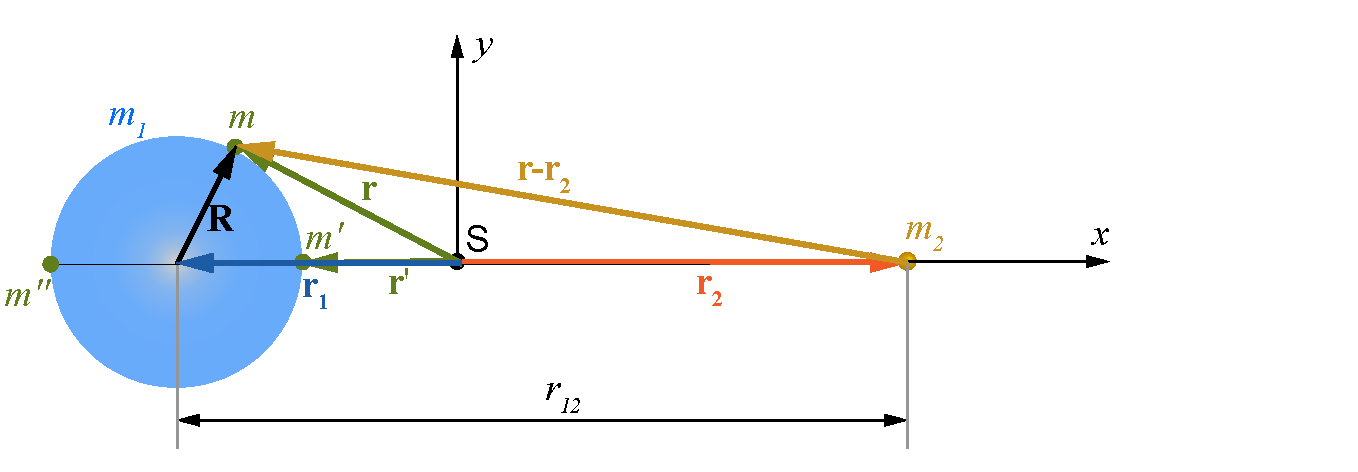
\includegraphics[width=\textwidth]{GeometrieGezeiten.pdf}%
\caption[Geometrie des Gezeitenproblems.]{Geometrie des Gezeitenproblems.}%
\label{abb:bew_3KoerperPGezeiten}%
\end{figure}

F�r das Erde-Mond-System kann man in guter N�herung $r_1=0,\,r_2=r_{12}=r_\text{EM}$ annehmen, f�r das Erde-Sonne-System in sehr guter N�herung $r_2 =0,\,r_1=r_{12}= r_\text{ES}$. Da die weiteren Betrachtungen auch \zb f�r Doppelsternsysteme anwendbar sein sollen, bei denen $m_1 \approx m_2$ gelten kann, schreiben wir allgemeiner

	\begin{align*}
			\vec{F}\!\lk\vec{r}\rk = -m\,\gradv\, U\lk\vec{r}\rk = -m\lk \frac{\d}{\d x}U\lk\vec{r}\rk, \frac{\d}{\d y}U\lk\vec{r}\rk, \frac{\d}{\d z}U\lk\vec{r}\rk\rk \,,
	\end{align*}
den Vektor $\vec{r}_1 = x\,\vec{e}_x+y\,\vec{e}_y+z\,\vec{e}_z$ , sowie das Skalarprodukt von $\delta\vec{r}$ und $\gradv$ als
	\begin{align*}
			\delta\vec{r}\cdot \gradv &= \D x\,\frac{\d}{\d x}+ \D y\,\frac{\d}{\d y}+\D z\,\frac{\d}{\d z} = \sum\limits_{i}^3 \D x_i\,\frac{\d}{\d x_i} = \D x_i\,\frac{\d}{\d x_i}\,.
	\end{align*}
Dann kann man die Gezeitenkraft \eqref{eq:bew_Gezeiten02} schreiben als
        \begin{align}
				\Delta \vec{F}_\text{Gez} &= \vec{F}\!\lk\vec{r}_1+\delta\,\vec{r}\rk-\vec{F}\!\lk\vec{r}_1\rk = \delta \vec{r}\cdot\gradv\vec{F}(\vec{r}_1) = -m \sum\limits_{i}^3 \sum\limits_{j}^3 \D x_j \, \frac{\d^2 U(\vec{r})}{\d x_i\,\d x_j }\,\vec{e}_i \nonumber \\
				&= -m\, \sum\limits_{i}^3 \sum\limits_{j}^3 \D x_j\,H_{ij} \,\vec{e}_i = -m\, \D x_j\,H_{ij} \,\vec{e}_i \,, \label{eq:bew_Gezeiten03}
\end{align}
wobei wir im letzten Schritt mit $\mathbb{H} \equiv H_{ij}$  ist die sogenannte Hesse-Matrix\footnote{Otto Hesse\indexp{Hesse, Otto} (1811--1874) war ein deutscher Mathematiker, der vor allem auf dem Gebiet der analytischen Geometrie arbeitete.} eingef�hrt und die Einsteinsche Summenkonvention benutzt haben. \\
Die vollst�ndige Hesse-Matrix in kartesischen Koordinaten ausgeschrieben lautet 
\begin{align}
	H_{ij} = \frac{\d^2 U}{\d x_i \d x_j} = 
\begin{pmatrix}
\frac{\d^2\, U}{\d\,x^2} & \frac{\d^2\, U}{\d x\,\d y}  & \frac{\d^2\, U}{\d x\,\d z} \\
\frac{\d^2\, U}{\d y\,\d x} & \frac{\d^2\, U}{\d\,y^2} & \frac{\d^2\, U}{\d y\,\d z} \\
\frac{\d^2\, U}{\d z\,\d x} & \frac{\d^2\, U}{\d z\,\d y} & \frac{\d^2\, U}{\d\,z^2}
\end{pmatrix} \,.
\label{eq:bew_Gezeiten04}
\end{align}
Gleichung \eqref{eq:bew_Gezeiten03} gilt ganz allgemein
f�r ein beliebiges \pot{}, \zb auch f�r eines mit mehreren Gravitationszentren,
und ist auch gut f�r die numerische Auswertung geeignet.
Man beachte aber, dass \eqref{eq:bew_Gezeiten03} eine Taylorentwicklung ist, weswegen f�r alle $i,j$ jeweils $\D x_j \ll \left| x_j - x_i \right| ~$ gelten muss. 
Wir wollen im Folgenden den einfachen Fall annehmen, dass die Testmasse auf der Verbindungsachse der beiden Massen $m_1$ und $m_2$ liegt.
Gleichung \eqref{eq:bew_Gezeiten03} sieht dann f�r die Masse $m'$ mit $\vec{r}' = \vec{r}_2-\vec{r}_1$ und $\delta\,\vec{r}\| \vec{r}'$ (wir betrachten ja nur die axiale Richtung) folgenderma�en aus:
		\begin{align}
				\Delta F_\text{Gez} = \Delta \vec{F}_\text{Gez}\cdot\vec{e}_z = \lk \frac{G\,m\,m_2}{\lk r_{12} \pm R_1\rk^2}\frac{\vec{r}}{|\vec{r}|} - \frac{G\,m\,m_2}{r_{12}{}^2}\frac{\vec{r}}{|\vec{r}|} \rk\cdot \vec{e}_z \,. \label{eq:bew_Gezeiten05}
		\end{align}
Da f�r den Radius des K�rpers mit der Masse $m_1$ aber $R \ll r_{12}$ gilt, k�nnen wir \eqref{eq:bew_Gezeiten05} entwickeln und erhalten
        \begin{align}
                \frac{1}{\lk r_{12} \pm R\rk^2}&\approx \frac{1}{r_{12}{}^2}\lk 1 \mp \frac{2R}{d}\rk \text{\quad und} \nonumber \\
                \Delta F_\text{Gez} &\approx \mp\frac{2G\,m\,m_2\,R}{r_{12}{}^3}\,.\label{eq:bew_Gezeiten06}
        \end{align}
Das Zeichen $+$ ist dabei f�r einen Probek�rper $m'$ zu verwenden,
der auf der Seite des ausgedehnten K�rpers liegt,
welche dem Ort der Masse $m_2$ zugewandt ist,
das Zeichen $-$ entsprechend f�r einen Probek�rper $m''$ auf der diesem Ort abgewandten Seite des K�rpers $m_1$.
Interessant ist der starke Abfall der Gezeitenkraft mit der dritten Potenz
des Abstandes zwischen den Massen $m_1$ und $m_2$.
Mit \eqref{eq:bew_Gezeiten06} kann man sofort das Verh�ltnis der Gezeitenkr�fte von Sonne und Mond auf einen K�rper auf der Erdoberfl�che berechnen:
		\begin{align*}
				\frac{\Delta {F_\text{Gez}}_\text{M}}{\Delta{F_\text{Gez}}_\text{S}} = \frac{m_\text{M}}{{a_{\text{EM}}}^3}\frac{{a_\text{ES}}^3}{m_\text{\text{S}}} \approx 2.18 \,.
		\end{align*}
Hier haben wir die Werte f�r die Mondmasse $m_\text{M} = \SI{7.346e22}{\kilogram}$, die Sonnenmasse $m_\text{S} = \SI{1.989e30}{\kilogram}$, den mittleren Abstand von Erde und Mond $a_\text{EM}= \SI{384.4e06}{\metre}$ und die sogenannte astronomische Einheit\index{Astronomische Einheit}\index{Astronomische Einheit} $a_\text{\earth} = a_\text{\text{ES}} = \SI{149.6e09}{\metre}$ benutzt.
Die Gezeitenwirkung des Mondes auf die Erde ist also etwa doppelt so gro� wie die der Sonne auf die Erde.
In \probref{bew_gezeiten01} wollen wir die Verformung eines Rings unter dem Einfluss von Gezeitenkr�ften berechnen. Den Ring beschreiben wir als Anordnung von 36 Testmassen, die im Schwerefeld einer gro�en Masse frei fallen.\\

\subsection{Lagrange-Formalismus}\index{Lagrange-Gleichung} \label{kap:bew_lagrange_formalism}

Bisher haben wir die Mechanik auf Basis der Newtonschen Axiome und der daraus folgenden Bewegungsgleichungen behandelt. Wir wollen jetzt den \emph{Lagrange-Formalismus}\index{Lagrange-Formalismus|textbf} kennen lernen, der 1788 von Lagrange\indexp{Lagrange, Joseph-Louis} eingef�hrt wurde und bei dem ein mechanisches System durch eine einzige skalare Funktion, die Lagrange-Funktion, beschrieben wird. Der Formalismus ist v�llig �quivalent zur Newtonschen Mechanik und ist dar�ber hinaus auch direkt auf beliebige Koordinatensysteme und beschleunigte Bezugssysteme anwendbar, ohne dass man eine zus�tzliche Betrachtung der Scheinkr�fte machen muss. Der Lagrange-Formalismus erlaubt damit die Wahl geeigneter generalisierter Koordinaten und vereinfacht dadurch die Behandlung vieler physikalische Probleme. Ebenso lassen sich im Gegensatz zur Newtonschen Mechanik Zwangsbedingungen relativ einfach ber�cksichtigen.

\subsubsection{Zwangsbedingungen}\index{Zwangsbedingungen} \label{kap:bew_zwangsbedingungen}

Die bisher gezeigten Anwendungen der Newtonschen Bewegungsgleichungen behandelten F�lle, in denen sich ein K�rper/Massepunkt frei, \dh nur unter dem Einfluss externer Kr�fte bewegen konnte.
H�ufig liegt aber Einschr�nkungen der Bewegungsfreiheit vor.
Eine solche nennt man dann eine \emph{\gls{zwangsbed}}.\footnote{Das kennen wir als Menschen ja auch sehr gut.} Zwangsbedingungen k�nnen f�r ein $N$-Teilchen-System in der Form
\begin{align}
	f_r(t, \vec{r_1},\vec{r_2},\ldots,\vec{r_N}) = 0 ~~, r = 1\ldots Z_B\,,\text{ wobei }Z_B \leq 3N  \label{eq:bew_holonome_ZB}
\end{align}
geschrieben werden, wodurch dann $ F = 3N -Z_B $ \emph{Freiheitsgrade}\index{Freiheitsgrad} der Bewegung verbleiben.
Als Beispiel sei die Bewegung auf einer schiefen Ebene genannt.
Da sich der Massepunkt entlang der Geraden $z = x \tan{\alpha}$ bewegen muss, lautet die Zwangsbedingung 
	\[f_1(0,x,y,z) = z - x \tan{\alpha} = 0
\]
und das System hat zwei verbleibende Freiheitsgrade $(x, y)$. Man kann nun unterscheiden in
\begin{itemize}
	\item \emph{holonom-skleronome} Zwangsbedingungen\index{Zwangsbedingung!holonom-skleronome}, die nicht explizit von der Zeit abh�ngen, also $\partial f_r/\partial t = 0$,
	\item \emph{holonom-rheonome} Zwangsbedingungen\index{Zwangsbedingung!holonom-rheonome}, die explizit von der Zeit abh�ngen, also $\partial f_r/\partial t \neq 0$,
	\item \emph{nicht-holonome} Zwangsbedingungen\index{Zwangsbedingung!nicht-holonome}, die sich nicht in der Form \eqref{eq:bew_holonome_ZB} schreiben lassen und daher die Anzahl der freien Koordinaten nicht reduzieren, wie 
	\begin{itemize}
		\item Zwangsbedingungen, die in der Form von Ungleichungen vorliegen, also 
			\[\tilde{f}(t, \vec{c}_1\cdot \D\vec{r_1},\vec{r_2},\ldots,\vec{r_N}) \leq 0
		\] 
		\item oder Zwangsbedingungen, die in nicht-integrierbarer differentieller Form 
			\[\delta \tilde{f} = \vec{c}_{k1}\cdot \D\vec{r_1} + \vec{c}_{k2}\cdot \D\vec{r_2} + \cdots + \vec{c}_{kN}\cdot  \D\vec{r_N} + \vec{c}_{kt} \D t = 0 \quad \text{mit}\quad k = 1 \ldots Z
		\]vorliegen.
                $\delta \tilde{f}$ ist dabei kein totales Differential.
	\end{itemize}
\end{itemize}
Wir werden in den \anf{Finger�bungen} Probleme mit verschiedenen Zwangsbedingungen untersuchen, dem Leser wird als Einstieg \probref{bew_Zwangsbedingungen} empfohlen.

%BEISPIEL 1 %%%%%%%%%%%%%%%%%%%%%%%%%%%%%%%%%%%%%%%%%%%%%%%%%%%%%%%%%%%%%%%%%%%%%%%%%%%%%%%%%%
\begin{example}{Beispiele f�r Zwangsbedingungen}
\begin{enumerate} [a)]
	\item holonom-skleronome Zwangsbedingung (\zb schiefe Ebene):
		\[f_1(t, x, y, z) = z- x \tan{\alpha} = 0
	\]
		\item holonom-rheonome Zwangsbedingung (\zb Pendelaufh�ngung an einer Decke, der Aufh�ngepunkt schwingt horizontal mit $\omega_\text{P}$)
		\[f_1(z, \varphi) = z + l \cos{\varphi} = 0 \quad\text{und}\quad \\
		  f_2(t, x, \varphi) = x - A \cos{\lk \omega_\text{P} t \rk} - l \sin{\varphi} = 0
	\]
	\item nicht-holonome Zwangsbedingung als Ungleichung (\zb beliebige Bewegung eines Massepunktes im Innenraum eines Kegels)
		\[ \tilde{f}_1(\rho, \varphi, z) = \rho - z \tan{\alpha} \leq 0\,,\quad 0 \leq \varphi \leq 2\pi
	\]
	\item nicht-holonome Zwangsbedingung als nicht-integrierbare differentielle Gleichung (\zb rollende Kugel mit der $x$-$y$-Ebene als Auflagefl�che)
		\[ \D x - \omega_2 R \D t = 0\,, \quad\D y - \omega_1 R \D t = 0   \quad\text{und} \quad\vec{\omega} = (\omega_1, \omega_2, \omega_3)  
	\]
\end{enumerate}
\begin{center}
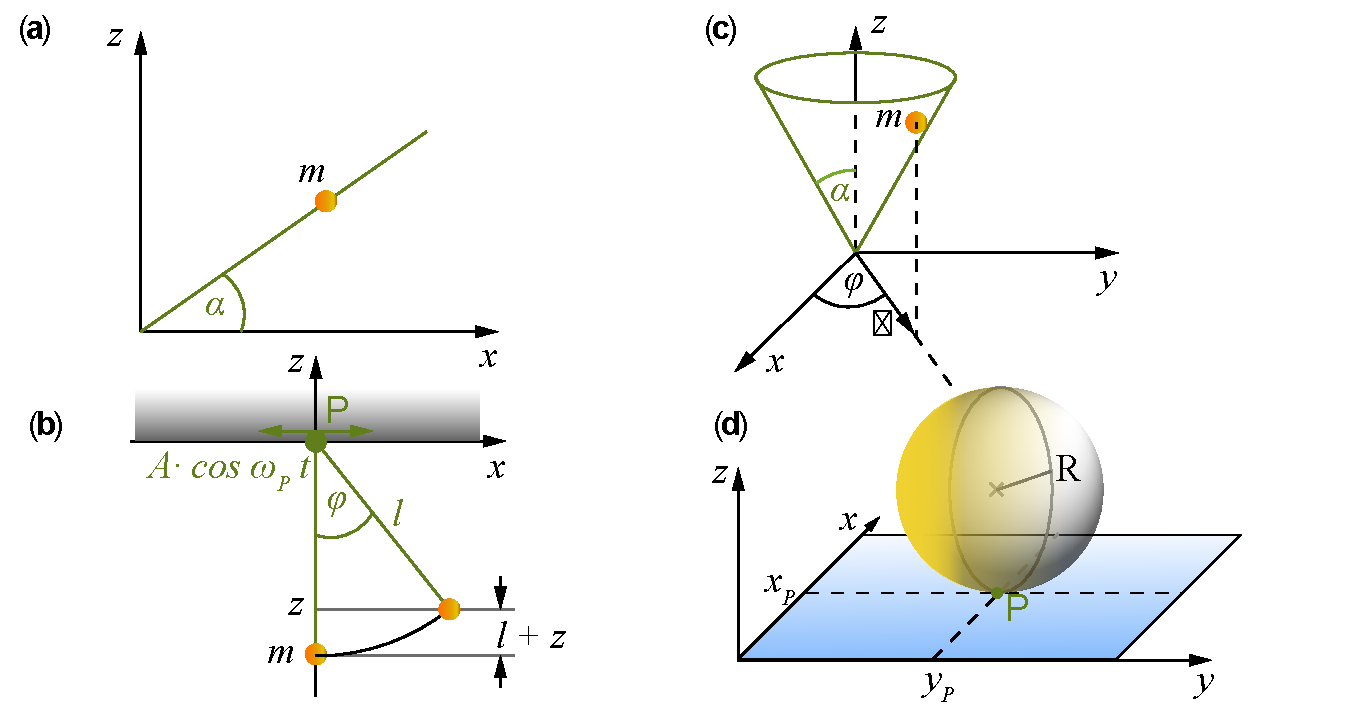
\includegraphics[width=\columnwidth]{ZwangsbedingungenBsp.pdf}% 
\captionof{figure}{Beispiele f�r Zwangsbedingungen (siehe Beispiel \ref{bsp:bew_ZB}).} \label{abb:bew_ZwangBedBsp}
\end{center}
\label{bsp:bew_ZB}
\end{example}
%Ende BEISPIEL %%%%%%%%%%%%%%%%%%%%%%%%%%%%%%%%%%%%%%%%%%%%%%%%%%%%%%%%%%%%%%%%%%%%%%%%%%%%%%%%%%

\subsubsection{Lagrange-Gleichungen erster Art}\index{Lagrange-Gleichung!Erster Art} \label{kap:bew_Lagrange_I}

Wenn die $Z_B$ holonomen Zwangsbedingungen zu jedem Zeitpunkt $t$ in einem System erf�llt sein sollen, muss man die Newtonsche Bewegungsgleichung durch eine \emph{\gls{zwangskr}}\index{Zwangskr�fte} erweitern, denn offensichtlich kann nur eine solche Kraft, die \zb von einer Unterlage oder einem Faden vermittelt wird, die Zwangsbedingung erf�llen.
Diese Kraft ist anders als die eingepr�gte �u�ere Kraft \ia zun�chst unbekannt.
Wir betrachten vorerst einen einzelnen Massepunkt und k�nnen dann die holonomen Zwangsbedingungen geometrisch als Fl�chen interpretieren, auf denen sich der Massepunkt bewegen soll.
Dann muss die Zwangskraft senkrecht auf dieser Fl�che stehen, was allgemein $\vec{Z} \propto \gradv f$ bedeutet.
Wir k�nnen deshalb die Bewegungsgleichung um den Proportionalit�tsfaktor $\lambda$ erweitern, den wir \emph{\gls{lagrmult}} nennen.
Die Zwangskr�fte sind dann
\begin{align}
	\vec{Z}_k &= \sum\limits_{r=1}^{Z_B}\lambda_r \gradv_k f_r \quad\text{\bzw in Komponenten} ~~\nonumber \\
	Z_k &= \sum\limits_{r=1}^{Z_B}\lambda_r \frac{\partial {f_r}}{\partial {x_k}}\,. \label{eq:bew_Zwangskraefte}
\end{align}
Die Bewegungsgleichungen, jetzt wieder erweitert auf $N$ Teilchen \bzw $3N$ Koordinaten, lauten dann
\begin{subequations}
\begin{align}
	m_k \ddot{\vec{r}}_k &= \vec{F}_k + \sum\limits_{r=1}^{Z_B}\lambda_r \gradv_k f_r \qquad k = 1 \ldots N ~~~~\text{\bzw} \\
	m_i \ddot{x}_i &= F_i + \sum\limits_{r=1}^{Z_B}\lambda_r \frac{\partial {f_r}}{\partial {x_i}}\qquad  i = 1 \ldots 3N\,. 
\end{align} \label{eq:bew_Lagrange_I}
\end{subequations}

Die Gleichungen \eqref{eq:bew_Lagrange_I} hei�en Lagrange-Gleichungen erster Art und stellen ein System von $3N$ Bewegungsgleichungen dar, in welchem die $Z_B$ Zwangsbedingungen �ber die Lagrange-Multiplikatoren $\lambda_r$ implizit enthalten sind.
Wir wollen noch kurz ohne Beweis erw�hnen, dass bei Vorliegen holonomer Zwangsbedingungen folgende Beziehung f�r die Energie gilt \cite{Kuypers2012, Bartelmann2015}:
\begin{align}
	\frac{\D}{\D t} E = 	\frac{\D}{\D t} (T+U) = - \sum\limits_{k=1}^{Z_B}\lambda_r \frac{\partial f_r}{\partial t}\,.\label{eq:bew_Lagrange_IE}
\end{align}
F�r skleronome Zwangsbedingungen ($\partial f_r / \partial t = 0$) bleibt also die Energie des Systems konstant, die Zwangskr�fte leisten in diesem Fall keine Arbeit.\\
Die Frage ist nun, wie man die Lagrange-Gleichungen erster Art l�st. F�r holonome Zwangsbedingungen gibt es folgende \textit{L�sungsstrategie}, deren konkrete Umsetzung wir in den Beispielen \ref{bsp:bew_PerleDraht} und \ref{bsp:bew_Rollenpendel} zeigen: \\ \\
\smallskip
\fbox{\parbox{0.95\textwidth}{
\smallskip
\textbf{\textit{Allgemeine L�sungsstrategie f�r Lagrange-Gleichungen erster Art mit holonomen Zwangsbedingungen �ber die Methode der Lagrange-Multiplikatoren}}
\begin{enumerate}
    \item Man stellt die Bewegungsgleichungen
      \eqref{eq:bew_Lagrange_I} und die Zwangsbedingungen
      $f_r(x_i,t)=0$ f�r die $3N$ Koordinaten $x_i$
      der $N$ Massepunkte auf.
    \item Man berechnet aus den Zwangsbedingungen die ersten und zweiten Ableitungen
      von $f_r(x_i,t)=0$:
      \begin{align}
         \dot{f}_r &= \sum\limits_{i=1}^{3N} \lambda_r \frac{\partial {f_r}}{\partial {x_i}} \dot{x}_i  + \frac{\partial {f_r}}{\partial t} \nonumber \\
        \ddot{f}_r &= \sum\limits_{i=1}^{3N} \lambda_r \frac{\partial {f_r}}{\partial {x_i}} \ddot{x}_i - a_r(t,x, \dot{x}) = 0\,.  \label{eq:bew_Lagrange_Ia}
      \end{align}
      Der Term $a_r(t,x, \dot{x})$ enth�lt alle Ableitungen
      von $f_r$ nach $t, x_i$ und $\dot{x}_i$, h�ngt aber nicht
      von den zweiten Ableitungen $\ddot{x}_i$ ab.
    \item Man setzt f�r die $\ddot{x}_i$
      in \eqref{eq:bew_Lagrange_Ia} die Bewegungsgleichungen \eqref{eq:bew_Lagrange_I} ein
      und erh�lt ein lineares inhomogenes Gleichungssystem
      f�r die $Z_B$ Lagrange-Multiplikatoren $\lambda_r$,
      welche in der impliziten Form 
      \begin{align}
          \lambda_r = \lambda_r(t, x, \dot{x})\,,\quad r = 1 \ldots Z_B \label{eq:bew_Lagrange_Ib}
      \end{align}
      berechnet werden k�nnen.
    \item Man setzt die impliziten Lagrange-Multiplikatore L�sungen \eqref{eq:bew_Lagrange_Ib} in die
      Bewegungsgleichungen \eqref{eq:bew_Lagrange_I} ein
      und erh�lt schlie�lich ein $3N$-dimensionales
      Differentialgleichungssystem zweiter Ordnung
      \begin{align}
	m_i \ddot{x}_i &= F_i + \sum\limits_{r=1}^{Z_B}\lambda_r(t, x, \dot{x}) \frac{\partial f_r}{\partial x_i}\,, \label{eq:bew_Lagrange_Ic}
      \end{align}
      das mit den �blichen Methoden zur L�sung von
      Differentialgleichungen (DGL)\index{Differentialgleichung}
      gel�st werden kann. 
    \item Mit den L�sungen kann man dann auch
      die Lagrange-Multiplikatoren und damit �ber
      \eqref{eq:bew_Zwangskraefte} die Zwangskr�fte berechnen,
      falls man diese explizit braucht.
      Zu beachten ist noch, dass alle Anfangsbedingungen
      den Zwangsbedingungen gen�gen m�ssen.\footnotemark
    \item F�r nicht-holonome Zwangsbedingungen gibt es kein allgemein g�ltiges Vorgehen. Wenn die nicht-holonomen Zwangsbedingungen in differentieller Form vorliegen, kann man die dargestellte Methode in leicht abgewandelter Form ebenfalls verwenden. 
		\item Wir werden die Methode der Lagrange-Multiplikatoren \zb in
 \probref{bew_unwucht}, \probref{bew_Trebuchet} \ua anwenden.
\end{enumerate}
}} 

\subsubsection{Verallgemeinerte Koordinaten}\label{kap:bew_general_coordinates}

In den (holonomen) Zwangsbedingungen \eqref{eq:bew_holonome_ZB} und den Lagrange-Gleichungen erster Art \eqref{eq:bew_Lagrange_I} haben wir zun�chst noch kartesische \bzw orthonormale Koordinaten (\zb Kugelkoordinaten) angenommen.
Deswegen mussten wir $3 N$ Komponentengleichungen l�sen und dabei $Z_B$ Zwangsbedingungen ber�cksichtigen.
Wir k�nnen uns die Aufgabe vereinfachen, indem wir zu sogenannten \emph{verallgemeinerten} oder \emph{generalisierten}\glslink{genkoord}{} Koordinaten \glslink{genkoord} �bergehen.
Diese Koordinaten $q_j$ werden als unabh�ngige Parameter entsprechend der Anzahl der \emph{Freiheitsgrade}\index{Freiheitsgrad} $F$ definiert und sind dann nicht mehr per Definition weiter durch Zwangsbedingungen eingeschr�nkt, da diese ja durch die entsprechende Auswahl der $q_j$ bereits ber�cksichtigt worden sind.
F�r holonome Zwangsbedingungen existiert dann folgende Beziehung:
\begin{align}
	x_i=x_i(t, q_j) \qquad i = 1\ldots 3N \quad j = 1 \ldots F\,. \label{eq:general_coordinates}
\end{align}
Diese verallgemeinerten Koordinaten k�nnen die Behandlung vieler Probleme der Mechanik (und auch anderer Themengebiete) deutlich vereinfachen, insbesondere dann, wenn man nicht an den Zwangskr�ften interessiert ist. 

\subsubsection{Lagrange-Gleichungen zweiter Art}\index{Lagrange-Gleichung!Zweiter Art} \label{kap:bew_Lagrange_II}

Wir beginnen mit \eqref{eq:general_coordinates}.
Die Zwangsbedingungen sind entsprechend der Bedingung
\begin{align}
	\frac{\partial{f_r}}{\partial{q_j}} = \sum\limits_{i}^{3N} \frac{\partial{f_r}}{\partial{x_i}} \frac{\partial{x_i}}{\partial{q_j}} \stackrel{!}{=} 0 \label{kap:bew_Zwangsbedingung_II}
\end{align}
ber�cksichtigt, denn wenn die Zwangsbedingungen von den $q_j$ abhingen, st�nde das im Widerspruch zur Definition der verallgemeinerten Koordinaten.
Multipliziert man die Lagrange-Gleichung erster Art mit ${\partial{x_i}}/{\partial{q_j}}$ erh�lt man:
\begin{align}
	\sum\limits_{i}^{3 N} m_i \ddot{x}_i \frac{\partial{x_i}}{\partial{q_j}} &= \sum\limits_{i}^{3 N} F_i \frac{\partial{x_i}}{\partial{q_j}} + \sum\limits_{r=1}^{Z_B}\lambda_r \sum\limits_{i}^{3N} \frac{\partial {f_r}}{\partial {x_i}} \frac{\partial {x_i}}{\partial {q_j}}\,. \label{eq:bew_Lagrange_II_a}
\end{align}
Der erste Term 
\begin{align}
	Q_j &= \sum\limits_{i}^{3N} F_i \frac{\partial {x_i}}{\partial {q_j}} \label{eq:bew_Lagrange_II_b}
\end{align}
ist offensichtlich eine Kraft und wird verallgemeinerte oder \emph{generalisierte Kraft}\index{Kraft!generalisierte}\index{Kraft!verallgemeinerte} genannt, w�hrend der zweite Term aufgrund der Bedingungen f�r die verallgemeinerten Koordinaten verschwindet.
Durch geeignete Umformung wie Vertauschung der partiellen Ableitungen und Einf�hrung \emph{generalisierter Geschwindigkeiten} $\dot{q}_j$ und der kinetischen Energie $T$
\begin{align}
	\dot{q}_j &= \frac{\D}{\D t} q_j\,, \quad T= \frac{1}{2} \sum\limits_{i}^{3N} m_i \dot{x}_i^2 \label{eq:bew_Lagrange_II_c}
\end{align}
erh�lt man nach einfachen Rechnungen (siehe \cite{Greiner2004, Bartelmann2015, Kuypers2012}) die \emph{Lagrange-Gleichungen zweiter Art}:
\begin{align}
	\frac{\D}{\D t} \frac{\partial T}{\partial \dot{q}_j} - \frac{\partial T}{\partial q_j} = Q_j \qquad j = 1 \ldots F\,. \label{eq:bew_Lagrange_II_d}
\end{align}
Die $Q_j$ sind zun�chst noch beliebige Kr�fte, sie k�nnen konservativ oder auch dissipativ sein.
Deshalb zerlegen wir diese in
	\[Q_j = Q_j^\text{(kons)} + Q_j^\text{(diss)}\,.
\]
Wir nehmen zun�chst nur konservative Kr�fte an und k�nnen dann schreiben:
	\[Q_j = Q_j^\text{(kons)} = \sum\limits_{i}^{3N} F_i \frac{\partial {x_i}}{\partial {q_j}} = -  \frac{\partial {U(t,x)}}{\partial {q_j}}\,,
\]
woraus schlie�lich mit der \emph{\gls{lagrfkt}} $\mathcal{L} = T -U $\index{Lagrange-Funktion|textbf} die Lagrange-Gleichungen zweiter Art f�r konservative Kr�fte folgen:
\begin{align}
	\mathcal{L} &= T - U = T(t, q_j, \dot{q}_j) - U(t, q_j) \nonumber \\
		\frac{\D}{\D t} \frac{\partial \mathcal{L}}{\partial \dot{q}_j} - \frac{\partial \mathcal{L}}{\partial q_j} &=  \left\{\frac{\D}{\D t} \frac{\partial }{\partial \dot{q}_j} - \frac{\partial}{\partial q_j} \right\} \mathcal{L} = 0 \qquad j = 1 \ldots F\,. \label{eq:bew_LagrangeGl_II}
\end{align}
Die Lagrange-Gleichungen sind $F$ Differentialgleichungen zweiter Ordnung f�r die $q_j(t)$.
Die allgemeine L�sung hat demnach demnach $2F$ Parameter \bzw Anfangsbedingungen.\\
W�hrend die Newtonschen Bewegungsgleichungen f�r kartesische Koordinaten formuliert wurden und relativ kompliziert auf andere Koordinatensysteme zu transformieren sind, ist der Lagrange-Formalismus koordinatenunabh�ngig.
Die generalisierten Koordinaten sind frei w�hlbar, solange sie den Zwangsbedingungen gen�gen.
Man kann also mit den Lagrange-Gleichungen zweiter Art die Bewegungsgleichungen direkt in nicht-kartesischen Koordinaten aufstellen, die Lagrange-Gleichungen zweiter Art sind \emph{forminvariant}\glslink{forminvar}.
Forminvarianz bedeutet, dass die Lagrange-Gleichungen zweiter Art beim �bergang von Koordinaten $q_j$ zu neuen Koordinaten $Q_j(t, q)$ in ihrer Form erhalten bleiben:
\begin{align*}
	q_j \rightarrow Q_j(t, q) \quad&\text{und} \quad \mathcal{L}(q_j, \dot{q}_j, t) \rightarrow \mathcal{L'}(Q_j, \dot{Q}_j, t) \\
				\frac{\D}{\D t} \frac{\partial \mathcal{L}}{\partial \dot{q}_j} - \frac{\partial \mathcal{L}}{\partial q_j} &= 0 \rightarrow  \frac{\D}{\D t} \frac{\partial \mathcal{L'}}{\partial \dot{Q}_j} - \frac{\partial \mathcal{L'}}{\partial Q_j}  = 0 \qquad j = 1 \ldots F\,.
\end{align*}
Diese Eigenschaft ist �u�erst vorteilhaft, wenn man Probleme in nicht-kartesischen Koordinatensystemen oder in Nicht-Inertialsystemen behandeln will (\probref{bew_LagrangeII_a}).

Wir f�hren jetzt noch den \emph{kanonischen} oder \emph{generalisierten Impuls}\index{Impuls!kanonischer} ein:
\begin{align}
	p_j = \frac{\partial \mathcal{L}}{\partial \dot{q}_j}\,.\label{eq:bew_Lagrange_II_f}
\end{align}
Wenn die Lagrange-Funktion\index{Lagrange-Funktion} $\mathcal{L}$ nicht von $q_j$ abh�ngt, dann ist der zugeh�rige kanonische Impuls $p_j$ eine Erhaltungsgr��e und die zugeh�rige Koordinate ist eine \emph{zyklische} Koordinate\glslink{zykkoord}.
Es ist bei Problemen oft vorteilhaft, gezielt nach zyklischen Koordinaten zu suchen, da die Erhaltungsgr��e $p_j = \text{const}$ einer ersten Integration der Bewegungsgleichung entspricht.
So f�hrt die zyklische Koordinate $q_j$, die dem Drehwinkel um eine feste Achse entspricht, auf die Erhaltung des Drehimpulses, \vgl dazu auch \kap{bew_ZKP_NZKF}.\\
Bevor wir auf L�sungsstrategien f�r die Lagrange-Gleichungen zweiter Art eingehen, wollen wir noch eine Betrachtung zur Energieerhaltung machen.
Wir definieren zun�chst die \emph{Hamilton\indexp{Hamilton, Sir William Rowan}\footnote{Sir William Rowan Hamilton (1805--1865) war ein irischer Mathematiker und Physiker und Royal Astronomer f�r Irland. 1835 gelang ihm eine Formulierung der Mechanik, die heute seinen Namen tr�gt und die fast 100 Jahre sp�ter wegweisend f�r den �bergang zur Quantenmechanik war. Im Rahmen dieses Buches k�nnen wir auf diese leider nicht eingehen. Wir verweisen auf die Literatur (\zb \cite{Simonyi2004, Greiner2004, Bartelmann2015, Kuypers2012}).}-Funktion}\index{Hamilton-Funktion}
\begin{align}
	\mathcal{H} = \sum\limits_{i} \dot{q}_i \frac{\partial \mathcal{L}}{\partial \dot{q}_i} -  \mathcal{L} =  \sum\limits_{i} p_i \dot{q}_i - \mathcal{L}\,. \label{eq:bew_Hamilton_Fkt}
\end{align}
Wie man leicht nachrechnen kann, ist f�r konservative Systeme,
geschwindigkeitsunabh�ngige \pot{}e und skleronome Zwangsbedingungen
die Hamilton-Funktion gleich der Gesamtenergie $E$ des Systems,
weswegen f�r die Gesamtenergie eines Systems oft auch das Symbol
$H$ verwendet wird.%
\footnote{Wir werden auch in der Himmelsmechanik (Band II, Kapitel 3) der allgemeinen (historischen) Konvention folgend f�r die Gesamtenergie $H$ benutzen.}
Wir wollen nun auch f�r Lagrange-Gleichungen zweiter Art eine \textit{L�sungsstrategie} aufzeigen.
Diese gilt f�r holonome Zwangsbedingungen und konservative Kraftfelder.
In den Beispielen \ref{bsp:bew_PerleDraht} und \ref{bsp:bew_Rollenpendel} zeigen wir das Vorgehen wiederum konkret.\\
~

\fbox{\parbox{0.95\textwidth}{
\medskip
\textbf{\textit{L�sungsstrategie f�r Lagrange-Gleichungen zweiter Art}}
\begin{enumerate}
	\item Man �berlegt sich die aus den $Z_B$ holonomen Zwangsbedingungen verbleibenden $F = 3 N - Z_B $ Freiheitsgrade des Systems und ordnet jedem Freiheitsgrad eine generalisierte Koordinate $q_j$ zu.
          Die explizite Form der Zwangsbedingungen $f_r(x_i,t)=0$ muss nicht unbedingt bekannt sein.
	\item Man �berpr�ft, dass die $q_j$ nicht durch Zwangsbedingungen eingeschr�nkt sind.
          Zwischen den kartesischen Koordinaten $x_i$ und den $q_j$ besteht folgender Zusammenhang:
		\[x_i =  x_i(t, q_1,q_2,\ldots, q_{F})\,.
	\]
	\item Man schreibt die Lagrange-Funktion $\mathcal{L} = T - U$ auf.
	\item Man sucht nach zyklischen Koordinaten.
          Die damit verbundenen Impulse $p_j$ sind Erhaltungsgr��en und damit erste Integrale der Bewegungsgleichungen.
	\item F�r die nichtzyklischen Koordinaten stelle man mit den Lagrange-Gleichungen zweiter Art \eqref{eq:bew_LagrangeGl_II} die Bewegungsgleichungen auf, die wiederum mit den �blichen Methoden (analytisch \bzw numerisch) zur L�sung von Differentialgleichungen gel�st werden k�nnen (siehe \kap{bew_einschub_DGL}). 
\end{enumerate}
}}
\medskip

\subsubsection{Lagrange-Gleichungen zweiter Art mit Reibung und externen Kr�ften}\label{kap:bew_Lagrange_II_R}


\subparagraph{Generalisierte externe Kr�fte}

Bisher hatten wir bei der Herleitung der Lagrange-Gleichungen zweiter Art ausschlie�lich konservative Kr�fte betrachtet und konnten damit die Kr�fte allein durch die potentielle Energie $U$ beschreiben. Um auch nicht-konservative Kr�fte im Lagrange-Formalismus ber�cksichtigen zu k�nnen, werden die Kr�fte in die jeweilige Richtung der generalisierten Koordinaten \glq{}projiziert\grq. Diese Kr�fte hatten wir schon als generalisierte Kr�fte \eqref{eq:bew_Lagrange_II_b} eingef�hrt:
\begin{align}
	  Q_j &= \sum\limits_{i}^{3N} F_i \frac{\partial {x_i}}{\partial {q_j}}\,. \label{eq:bew_gen_Kraft_neu}
\end{align}


\subparagraph{Dissipationsfunktion}

Die dissipativen Kr�fte (also Kr�fte, die dem System Energie entziehen) k�nnen ebenfalls als generalisierte Kraft im Lagrange-Formalismus ber�cksichtigt werden. Alternativ kann man eine \emph{Dissipationsfunktion} $U_\text{R}$ einf�hren. Wir starten dazu von den generalisierten Reibungskr�ften\index{Reibungskr�fte!generalisierte} $F_{\text{R}j}$, die sich gem�� \eqref{eq:bew_Lagrange_II_b} \bzw \eqref{eq:bew_gen_Kraft_neu} �ber 
\begin{align}
	F_{\text{R}j} = \sum\limits_{k=1}^{N} \vec{F}_{\text{R}k} \cdot \frac{\partial \vec{r}_k}{\partial q_j} \label{eq:bew_gen_Reibungskraft}
\end{align}
aus den kartesischen Reibungskr�ften berechnen lassen. 
Wir hatten in \kap{bew_newton_axioms} gesehen, dass in der Mechanik vielfach die Reibungskraft proportional zur Geschwindigkeit ist, sodass $\vec{F}_{\text{R}k} = - \beta_k(v_k) \vec{v}_k/v_k$ gilt.
F�r solche Kr�fte kann ein \emph{Dissipations\potsuf{}}\index{Dissipationspotential}\index{Potential!Dissipationspotential} (auch Dissipationsfunktion\index{Dissipationsfunktion} genannt) definiert werden:
\begin{align}
	U_\text{R} &= \sum\limits_{k=1}^{N} \int\limits_{0}^{v_k} \beta_k(v_k') \:\D v_k' ~~~~\rightarrow~~~ F_{\text{R}j} = - \frac{\partial U_\text{R}}{\partial \dot{q}_j}\,.\label{eq:bew_Dissipationspotential}
\end{align}
Die negativen partiellen Ableitungen der Dissipationsfunktion nach den generalisierten Geschwindigkeiten m�ssen nat�rlich wieder die generalisierten Kr�fte der dissipativen Kr�fte ergeben.

Verallgemeinert berechnet sich das Dissipationspotential f�r die verschiedenen Reibungsarten nach:
\begin{itemize}
    \item \textit{Gleitreibung}: $U_{\text{R}_1} = \mu\,F_\text{N}\,|\vec{v}_\text{rel}|^1$,\,mit $\mu$ als Gleitreibungskoeffizient, $F_\text{N}$ ist die Normalkraft,
    \item \textit{Stokes-Reibung}\index{Stokes-Reibung}\index{Reibung!Stokes-}: $U_{\text{R}_2} = \frac{1}{2}\,\eta\,|\vec{v}_\text{rel}|^2$,\,mit $\eta$ als D�mpfungskonstante,
    \item \textit{Newton-Reibung} (\zb Luftwiderstand): $U_{\text{R}_3} = \frac{1}{3}\,c_w\,|\vec{v}_\text{rel}|^3$,\, mit $c_w$ als Luftwiderstandsbeiwert.
\end{itemize}

Damit lauten bei Vorliegen externer (nicht-konservativer) Kr�fte und eines Dissipations\potsuf{}s die Lagrange-Gleichungen zweiter Art:
\begin{align}
			&\frac{\D}{\D t} \frac{\partial \mathcal{L}}{\partial \dot{q}_j} &- \frac{\partial \mathcal{L}}{\partial q_j} + \frac{\partial U_\text{R}}{\partial \dot{q}_j} = Q_\text{j} ~~~~j= 1, \ldots, F\\
    &\text{Hierin sind f�r ein System mit}~~ F ~~\text{Freiheitsgeraden:} \notag \\
    q_j~~~&\text{die generalisierte Koordinaten,} \notag\\
		\dot{q}_j~~~&\text{die generalisierte Geschwindigkeiten,}\notag \\
    U_\text{R}~~~&\text{die Dissipationsfunktion und }\notag \\
		Q_j~~~&\text{die generalisierte Kr�fte}.\notag
\end{align} \label{eq:bew_LagrangeGl_II_Reibung}

\subsubsection{Anwendung des Lagrange-Formalismus auf Schwingungen}\index{Schwingung} \label{kap:bew_schwingung}

Schwingungen sind Bewegungen um eine Gleichgewichtslage herum.
Sie sind extrem wichtig in der Physik und besonders die harmonischen Schwingungen waren von grundlegender Bedeutung in der Weiterentwicklung der klassischen Mechanik hin zur Quantenmechanik.  Da sich fast alle Kr�fte lokal linearisieren lassen, spielen harmonische Schwingungen beispielsweise in der Akustik, der Festk�rper- und Quantenphysik und auch der Spektroskopie eine gro�e Rolle. 
Wir wollen uns zun�chst auf Schwingungen mit einem Freiheitsgrad beschr�nken.
Der Lagrange-Formalismus l�sst sich hierbei vorteilhaft anwenden.
Wir werden diesen dann auch auf mehrere Freiheitsgrade und Systeme von mehreren schwingenden Massepunkten erweitern.
In diesem Zusammenhang werden wir annehmen, dass alle Teilchen nur unter der Wirkung rein konservativer Kr�fte liegen.\\
Dabei gehen wir direkt zu einer generalisierten Koordinate $q$ �ber und untersuchen nun die spezielle Situation, dass der Ort $q$ des Teilchens nur wenig von einer stabilen Gleichgewichtslage $q_0$ abweicht.
\emph{Gleichgewicht}\index{Gleichgewicht} in der Position $q_0$ bedeutet, dass dort die Summe aller auf den Massepunkt wirkenden (generalisierten) Kr�fte gleich Null ist.
\emph{Stabilit�t}\index{Stabilit�t} bedeutet, dass f�r kleine Auslenkungen $q-q_0$ und geringe Impulse r�cktreibende Kr�fte wirken, die ein unbegrenztes Anwachsen der Auslenkung verhindern.
\begin{align*}
	F = -\frac{\partial U}{\partial x} 
\end{align*}
Das \pot{} kann im Allgemeinen eine beliebige Gestalt annehmen.
In vielen F�llen besitzt das \pot{} jedoch ein lokales Minimum bei $q_0$ (dem Ort der Gleichgewichtslage).
Wir entwickeln daher das \potz{} um das Minimum bei $q_0$ und erhalten:
\begin{align}
	U = U(q_0) + \frac{\d U}{\d q}\bigg|_{q_0}\cdot(q-q_0) + \frac{1}{2} \frac{\d^2 U}{\d q^2}\bigg|_{q_0}\cdot(q-q_0)^2 + \sum\limits_{k=3}^\infty \frac{1}{k!} \frac{\d^k U}{\d q^k}\bigg|_{q_0}\cdot(q-q_0)^k \label{eq:bew_Schwingung_a}
\end{align}
Als konstanter Wert des \potz{}s ist der erste Term irrelevant,
Der zweite Term ist Null, da das \potz{} um sein Minimum entwickelt wurde.
In vielen Anwendungen spielt bei kleinen Auslenkungen nur der quadratische Term in $q$ eine Rolle,  alle weiteren Terme werden ignoriert.
Dies f�hrt auf das \pot{} einer \emph{harmonischen} Schwingung\index{Schwingung!harmonische}.
Bei gr��eren Auslenkungen muss das \potz{} mit weiteren Termen der Entwicklung \eqref{eq:bew_Schwingung_a} ber�cksichtigt werden, was auf \emph{anharmonische	}\index{Schwingung!harmonische} Schwingungen f�hrt.\\
F�r die Aufstellung der Lagrange-Funktion ben�tigen wir noch die kinetische Energie, die definiert ist als
\begin{align*}
T &= \frac{1}{2}m \sum\limits_{i}^{3}{\dot{x}_i{}}^2 = \frac{1}{2} m \sum\limits_{i}^{3}\ \lk \sum\limits_{j}^{F} \frac{\partial x_i}{\partial q_j} \dot{q} \rk ^2 \,.
\end{align*}
F�r eindimensionale Bewegungen mit nur einer generalisierten Koordinate hei�t das:
\begin{align*}
	T &= \frac{1}{2}m \dot{x}^2 = \frac{1}{2} m \,  \dot{q}^2 \lk \frac{\partial x}{\partial q}\rk^2 =\: \frac{1}{2} m \,\dot{q}^2 \,h(q) \,.
\end{align*}
Den Ausdruck $h(q) = \lk\frac{\partial x}{\partial q}\rk ^2$ kann man ebenfalls um $q_0$ entwickeln und erh�lt
\begin{align}
	 T(q,\dot{q}) = \frac{m \dot{q}^2}{2} \lek h(q_0) + \sum\limits_{k=1}^\infty \frac{1}{k!} \frac{\d^k h(q)}{\d q^k}\bigg|_{q_0}\,(q-q_0)^k  \rek \,. \label{eq:bew_Schwingung_b}
\end{align}
Da der Vorfaktor bereits von zweiter Ordnung in $\dot{q}$ ist, muss bei geringen Auslenkungen in der Reihenentwicklung von $h(q)$ nur der konstante Beitrag ber�cksichtigt werden, vorausgesetzt $\dot{q}$ und $q$ sind von der gleichen Gr��enordnung, was bei kleinen Schwingungsamplituden der Fall ist.
Im diesem Grenzfall lautet die Lagrange-Funktion
\begin{align}
\mathcal{L} = T(q,\dot{q}) - U(q) = \frac{\tilde{m}}{2}\dot{q}^2 - \frac{1}{2} \frac{\partial^2 U}{\partial q^2}\bigg|_{q_0}\, q^2 \,,\label{eq:bew_Schwingung_c}
\end{align}
wobei wir $\tilde{m} = h(q_0) m$ benutzt haben.
Das ist die Schwingungsgleichung f�r eine harmonische Schwingung wie beim Federpendel, was unmittelbar einsichtig ist, wenn man $x=q$ setzt. \\

F�r anharmonische Schwingungen\index{Schwingung!anharmonische} ergibt sich die Lagrange-Funktion aus der Mitnahme weiterer Terme von \eqref{eq:bew_Schwingung_a} und \eqref{eq:bew_Schwingung_b}.
Wenn wir ein symmetrisches \pot{} um $q_0$ annehmen, gilt in der n�chsten N�herung:
\begin{align}
	\mathcal{L} = T - U & = \frac{m}{2}\dot{q}^2 \lek h(q_0) + (q-q_0) \frac{\d h(q)}{\d q}\bigg|_{q_0} + \frac{1}{2} \,(q-q_0)^2 \frac{\d^2 h(q)}{\d q^2}\bigg|_{q_0} \rek \nonumber \\
	          & \quad - \frac{1}{2} (q-q_0)^2 \lek \frac{\d^2 U}{\d q^2}\bigg|_{q_0}  -  \frac{1}{12} \frac{\d^4 U}{\d q^4}\bigg|_{q_0}\, (q-q_0)^2 \rek \,. \label{eq:bew_Schwingung_d}
\end{align}
Die aus \eqref{eq:bew_Schwingung_c} �ber die Lagrange-Gleichungen abgeleitete Schwingungsgleichung\footnote{Dies ist eine lineare Differentialgleichung mit konstanten Koeffizienten, weswegen man auch den N�herungs�bergang zu \eqref{eq:bew_Schwingung_c} auch als Linearisierung\index{Linearisierung} bezeichnet.} f�r die generalisierte Koordinate im Grenzfall geringer Schwingungen lautet
\begin{align}
	  \ddot{q} + \omega_0^2 \,q \:=\: 0 \,. \label{eq:bew_Schwingung01a}
\end{align}
F�r beliebig starke Schwingungen gilt allgemein:
\begin{align}
	  m \frac{\D}{\D t}\lk h(q) \,\dot{q} \rk - \frac{m \dot{q}^2}{2} \frac{\d h}{\d q} + \frac{\d U}{\d q} = 0 \,, \label{eq:bew_Schwingung01b}
\end{align}
worin $ h(q)$ eine Funktion allein von $q$ ist, die sich gem�� \eqref{eq:bew_Schwingung_b} berechnen l�sst.

\subparagraph{\textbf{Schwingungen und Dissipation}} 

In vielen Anwendungen treten bei Schwingungen dissipative Kr�fte auf, die zu einer D�mpfung der Schwingung f�hren.
Wir wollen den Einfluss einer solchen D�mpfung im Folgenden mit ber�cksichtigen und dabei zun�chst annehmen, dass die generalisierte dissipative Kraft linear in $\dot{q}_j$ ist, was \zb f�r die Stokes-Reibung \eqref{eq:bew_StokesReibung} gilt.
Wir k�nnten im Lagrange-Formalismus starten und das generalisierte \pot{} der Reibung berechnen.
Der Einfachheit halber gehen wir aber direkt von den Bewegungsgleichungen \eqref{eq:bew_Schwingung01a} \bzw \eqref{eq:bew_Schwingung01b} aus und addieren eine in $\dot{q}_j$ lineare Reibungskraft:
\begin{align}
	\ddot{q} + \beta \dot{q} + \omega_0^2 \,q \:=\: 0 \,.\label{eq:bew_Schwingung02}
\end{align}
Dieser lineare Fall ist in vielen F�llen eine gute Beschreibung der Realit�t. 
Bei \eqref{eq:bew_Schwingung02} handelt es sich ebenfalls um eine gew�hnliche lineare homogene DGL zweiter Ordnung.
F�r derartige Probleme kann man den von Euler gefundenen Exponentialansatz mit komplexen Zahlen 
\begin{align}
	Q(t) = \mathrm{e}^{\mathrm{i} \omega t} \label{eq:bew_Schwingung03}
\end{align}
verwenden und die allgemeine L�sung rasch erhalten: 
\begin{align}
  \lk -\omega^2 + \mathrm{i} \beta \omega + \omega_0^2 \rk \mathrm{e}^{\mathrm{i} \omega t}\,. \label{eq:bew_Schwingung04}
\end{align}
Die Bewegungsgleichung kann nur erf�llt werden, wenn der Term in der Klammer verschwindet.
Reibungsterme, die quadratisch in $\dot{q}_j$ sind, machen die mathematische Behandlung wesentlich anspruchsvoller, da die Bewegungsgleichung dann nicht mehr linear ist.
In der Regel werden wir diese dann numerisch l�sen m�ssen.


\subsubsection{Vergleichende Darstellung der L�sung der Bewegungsgleichung nach den Lagrange-Gleichungen erster und zweiter Art} \label{kap:bew_Lagrange_GlIV}

Wir wollen im Folgenden zwei instruktive Beispiele zur Anwendung der Lagrange-Gleichungen erster und zweiter Art zeigen.
Die Beispiele folgen den in den Kapiteln \ref{kap:bew_Lagrange_I} und \ref{kap:bew_Lagrange_II} gezeigten L�sungsstrategien und dienen als guter Einstieg in die �bungen.

\begin{figure}
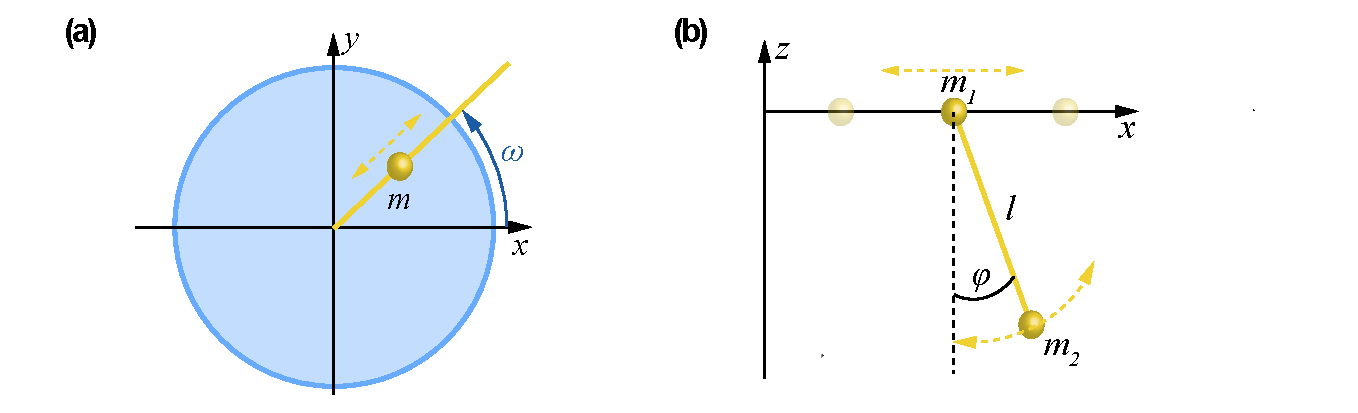
\includegraphics[width=\columnwidth]{RollenPendel.pdf}% 
\caption[Beispiele zum Lagrange-Formalismus.] {Beispiele zum Lagrange-Formalismus. \fa Rotierende Scheibe mit gleitender Perle auf Draht und \fb Rollenpendel.}
\label{abb:bew_Rollenpendel}
\end{figure}

\subparagraph{\textbf{Rotierende Scheibe mit gleitender Perle auf Draht}} 

Als erstes Beispiel wollen wir anhand eines Standardbeispiels aus vielen Lehrb�chern den Vergleich der beiden Methoden darstellen.
Wir haben hier ein Problem eines einzelnen Massepunktes unter Zwangskr�ften und Scheinkr�ften, da ein Nicht-Inertialsystem vorliegt (siehe \figref{bew_Rollenpendel}a). 

%BEISPIEL %%%%%%%%%%%%%%%%%%%%%%%%%%%%%%%%%%%%%%%%%%%%%%%%%%%%%%%%%%%%%%%%%%%%%%%%%%%%%%%%%%
\begin{example}{Zwangsbedingungen - Beispiel rotierende Scheibe mit gleitender Perle auf Draht}
\smallskip
\begin{itemize}
	\item \emph{L�sung mittels der Lagrange-Gleichungen erster Art}\\
	Wir betrachten nur die $x$-$y$-Ebene und verwenden Polarkoordinaten (Zylinderkoordinaten mit $z=0$).
        Dann gibt es nur eine Zwangsbedingung und nur einen Lagrange-Multiplikator $\lambda$:
			\[ f_1(\varphi) = \varphi - \omega t = 0 \]
Die Lagrange-Gleichung erster Art lautet dann
	\[m \ddot{\vec{r}} = \lambda \: \gradv f\,.
\]
Mit den Beziehungen f�r die Beschleunigung und den Gradienten f�r Zylinderkoordinaten k�nnen wir schreiben
\begin{align}
		m \lk \ddot{\varrho} - \varrho \dot{\varphi}^2 \rk \vec{e}_\varrho + m \lk \varrho \ddot{\varphi} + 2 \dot{\varrho} \dot{\varphi} \rk \vec{e}_\varphi = \lambda \frac{\partial f}{\partial\varrho} \vec{e}_\varrho + \lambda\frac{1}{\varrho}\frac{\partial f}{\partial\varphi} \vec{e}_\varphi\,. \label{eq:bew_PerleDraht_1}
\end{align}
Da $\partial f/\partial\varrho = 0$, $\partial f/\partial\varphi = 1$ und $\ddot{f} = \ddot{\varphi} = 0$, folgen wegen der notwendigen Gleichheit der Koeffizienten vor den Einheitsvektoren in \eqref{eq:bew_PerleDraht_1}
\begin{align}
\lambda &= 2 m \varrho \dot{\varrho} \dot{\varphi}\,, \nonumber \\
m \lk \ddot{\varrho} - \varrho \dot{\varphi}^2 \rk &= 0 \quad \text{und} \quad m \varrho \ddot{\varphi} = 0\,.\label{eq:bew_PerleDraht_2}
\end{align}
Daraus ergibt sich wegen $\dot{f} = \dot{\varphi} - \omega = 0$ die Bewegungsgleichung f�r $\varrho$
	\[\ddot{\varrho} - \omega^2 \varrho = 0\,,
\]
deren L�sung 
\begin{align}
        \varrho (t) = A \mathrm{e}^{+\omega t} + B \mathrm{e}^{-\omega t} \label{eq:bew_PerleDraht_3}
\end{align}
lautet, wobei sich $A$ und $B$ aus den Anfangsbedingungen ergeben.
Die Perle wird sich f�r $A \neq 0$ also mit der Zeit zu immer gr��eren Radien bewegen.
Die Zwangskraft 
	\[\vec{Z} = \lambda \:\vec{\nabla} f = 2\: m \:\dot{\varrho}\: \omega \: \vec{e}_\varphi
\]
leistet wegen \eqref{eq:bew_Lagrange_IE} eine Arbeit von
	\[\frac{\partial T}{\partial t} = - \lambda \frac{\partial f}{\partial t} = 2\: m \varrho \dot{\varrho} \omega^2 
\]
am System.\\
	\item \emph{L�sung mittels der Lagrange-Gleichungen zweiter Art}\\
	Die Lagrange-Funktion hat wegen der Zwangsbedingung nur die generalisierte Koordinate $\varrho$ und lautet in Zylinderkoordinaten mit $z=0$
\begin{align}
		\mathcal{L} = T = \frac{m}{2} \lk \dot{\varrho}^2 + \varrho^2 \dot{\varphi}^2 \rk\,.\label{eq:bew_PerleDraht_4}
\end{align}
Die Lagrange-Gleichungen ergeben nat�rlich wieder \eqref{eq:bew_PerleDraht_2}.
Man sieht, wie einfach und elegant der Formalismus mit der Lagrange-Gleichung zweiter Art ist.
In \probref{bew_LagrangeII_b} werden wir das Problem noch etwas ausf�hrlicher untersuchen und auch auf F�lle mit Reibung und ver�nderlicher Drehzahl der Scheibe erweitern.
Auch sei hier darauf hingewiesen, dass die Energie des Systems nicht erhalten ist, denn die Zwangsbedingung ist ja skleronom, mithin leistet die Zwangskraft keine Arbeit.
\end{itemize}
\label{bsp:bew_PerleDraht}
\end{example}
%BEISPIEL %%%%%%%%%%%%%%%%%%%%%%%%%%%%%%%%%%%%%%%%%%%%%%%%%%%%%%%%%%%%%%%%%%%%%%%%%%%%%%%%%%

\subparagraph{\textbf{Rollenpendel}} 

Als zweites Beispiel wollen wir anhand eines weiteren Standardbeispiels aus den Lehrb�chern wiederum den Vergleich der beiden Methoden darstellen.
Das Rollenpendel (\figref{bew_Rollenpendel}b) besteht aus zwei gekoppelten Massepunkten.
Die Masse $m_1$ kann sich nur auf einer Schiene entlang der $x$-Achse (reibungsfrei) bewegen.
Die Masse $m_2$ ist starr �ber einen masselosen Stab mit der Masse $m_1$ verbunden und kann sich nur in der $x$-$z$-Ebene bewegen.
Es liegt hier also ein Problem eines Systems von zwei Massepunkten mit Zwangskr�ften (im Inertialsystem) vor. 

%BEISPIEL %%%%%%%%%%%%%%%%%%%%%%%%%%%%%%%%%%%%%%%%%%%%%%%%%%%%%%%%%%%%%%%%%%%%%%%%%%%%%%%%%%
\begin{example}{\textbf{Beispiel f�r Zwangsbedingungen - Das Rollenpendel}}
\smallskip
\begin{itemize}
	\item \emph{L�sung mittels der Lagrange-Gleichungen erster Art}\\ 
	Hier gehen wir einen leicht ver�nderten Weg, indem wir zur Herleitung der Bewegungsgleichungen die Lagrange-Funktion benutzen.
        Wir haben vier Koordinaten (in der $x$-$z$-Ebene) und zwei Zwangsbedingungen.
        Als Koordinaten f�r $m_1$ w�hlen wir $x_1, z_1$ und f�r $m_2$ sinnvollerweise die Polarkoordinaten $r, \varphi$.
        Dann gelten folgende Zwangsbedingungen und Beziehungen mit $l$ als fester Pendell�nge: 
		\[ f_1(x_1, z_1; r, \varphi) = z_1 = 0  \quad\text{und}\quad \frac{\partial f_1}{\partial z_1} = 1 \; , \]
		\[ f_2(x_1, z_1; r, \varphi) = r - l = 0 \quad\text{und}\quad \frac{\partial f_2}{\partial r} = 1 \; . \]
	Alle anderen Ableitungen von $f_r$ verschwinden.
        Wir bilden jetzt die Lagrange-Funktion $\mathcal{L}'(x_1,z_1,\dot{x}_1, \dot{z}_1,r, \varphi, \dot{r}, \dot{\varphi})$ und bestimmen aus dieser die Bewegungsgleichungen. 
		\[\mathcal{L}'= \frac{m_1}{2}\lk \dot{x}_1^2 +\dot{z}_1^2 \rk + \frac{m_2}{2}\lk \dot{x}_2^2 +\dot{z}_2^2 \rk - m_1 \:g\: z_1 \:- \:m_2 \:g \:z_2
	\]
	Die Lagrange-Funktion enth�lt noch keine Zwangsbedingungen.
        Wir brauchen noch die $x_2$ und $z_2$ als Funktionen von $r$ und $\varphi$.
        Man liest aus der \figref{bew_Rollenpendel}b mit $M = m_1 + m_2$ ab:
		\begin{align*}
		  x_2 &= x_1 + r \sin\varphi  ~~\rightarrow~~\dot{x}_2 = \dot{x}_1 + \dot{r} \sin\varphi + r \dot{\varphi} \cos\varphi \\
		  z_2 &= z_1 - r \cos\varphi  ~~\rightarrow~~\dot{z}_2 = \dot{z}_1 - \dot{r} \cos\varphi + r \dot{\varphi} \sin\varphi \\
			\rightarrow \mathcal{L}' &= \frac{M}{2} \lek \dot{x}_1^2 + \dot{z}_1^2 \rek  \\
						 &+ \frac{m_2}{2} \lek \dot{r}^2 + \dot{\varphi}^2 r^2 + 2 \dot{r} \lk \dot{x}_1 \sin\varphi - \dot{z}_1 \cos\varphi \rk + 2 r\dot{\varphi} \lk \dot{x}_1 \cos\varphi + \dot{z}_1 \sin\varphi \rk \rek \\
						 &- m_1 \:g\: z_1 - m_2 \:g \lk z_1 - r\cos\varphi \rk\,.
		\end{align*}
		Auf dem �blichen Weg �ber die Lagrange-Gleichungen zweiter Art
                bestimmt man die Bewegungsgleichungen, in die man
                erst jetzt die Zwangsbedingungen und die Lagrange-Multiplikatoren einsetzt,
                von denen nur f�r $z_1 (\lambda_1)$ und $r (\lambda_2)$
                die Parameter $\lambda_i$
                von 0 verschieden sind.
                Es ergeben sich dann vier Bewegungsgleichungen.
                Die Gleichungen f�r $\ddot{x}_1$ und $\ddot{\varphi}$ enthalten logischerweise keine Zwangskr�fte:
		\begin{align}
			&M \ddot{x}_1 + m_2 \: l \lk \ddot{\varphi} \cos\varphi \: - \dot{\varphi}^2 \sin\varphi \rk = 0\,, \label{eq:bew_RollPendel_1} \\
			&m_2 \: l \lk l\: \ddot{\varphi} +  \ddot{x}_1 \cos\varphi + g \sin\varphi \rk = 0\,. \label{eq:bew_RollPendel_2}
		\end{align}
Diese sind im Prinzip nach $x_1(t)$ und $\varphi(t)$ -- wenn auch nur numerisch -- aufl�sbar, wobei $x_1(t)$ eine zyklische Koordinate ist und f�r $\varphi(t)$ zur Berechnung der Energieerhaltungssatz benutzt werden kann, da ja holonome Zwangsbedingungen vorliegen.
Die beiden anderen Bewegungsgleichungen lauten
		\begin{align}
                  &m_2 \: l \lk \ddot{\varphi} \sin\varphi + \dot{\varphi}^2 \cos\varphi \rk + M \: g = \lambda_1 = Z_\text{Schiene}\text{ und}\label{eq:bew_RollPendel_3} \\
                  &m_2 \lk \ddot{x}_1 \sin\varphi - l \: \dot{\varphi}^2 - g \cos\varphi \rk = \lambda_2 = -Z_\text{Stange}\,. \label{eq:bew_RollPendel_4}
		\end{align}
Die beiden Zwangskr�fte sind aus den L�sungen f�r $x_1(t)$ und $\varphi(t)$ auch mit der Erweiterung f�r Reibungskr�fte berechenbar (\probref{bew_LagrangeII_b}).
Man kann noch, indem man \eqref{eq:bew_RollPendel_2} in \eqref{eq:bew_RollPendel_3} einsetzt, einen Zusammenhang zwischen der Auflagekraft auf der Schiene und der Zugkraft in der Stange herstellen,
	\[ Z_\text{Schiene} = m_1 \: g + Z_\text{Stange} \cos\varphi\,,
\]
was sofort einsichtig ist.
Wir werden gleich sehen, dass die Lagrange-Gleichungen zweiter Art viel einfacher zu handhaben sind.
Der Vollst�ndigkeit halber sei noch darauf hingewiesen, dass man nat�rlich die Bewegungsgleichungen \eqref{eq:bew_RollPendel_1}--\eqref{eq:bew_RollPendel_4} auch ohne die Lagrange-Funktion $\mathcal{L}'$ aufstellen kann.
Entsprechend \kap{bew_Lagrange_I} bildet man zun�chst die partiellen Ableitungen $\partial f_r/ \partial x_i$ sowie die zeitlichen Ableitungen der Zwangsbedingungen $\dot{f}_r$ und $\ddot{f}_r$ und berechnet die Lagrange-Multiplikatoren $\lambda_r(t, x_i, \dot{x}_i)$, die man in die Bewegungsgleichungen einsetzt.
Dem Leser ist dieses Vorgehen als �bung empfohlen.
	\item \emph{L�sung mittels der Lagrange-Gleichungen zweiter Art}\\
	Mit den Zwangsbedingungen $f_1(x_i, z_i) = z_1 = 0$ und $f_2(x_i, z_i) = (x_1 -x_2)^2 + z_2^2 - l^2 = 0 $ und den Beziehungen $ x_2 = x_1 + l\sin\varphi $ \bzw $ z_2 = l\cos\varphi$ schreiben wir die Lagrange-Funktion $\mathcal{L}$ in den generalisierten Koordinaten $q_1 = x_1$ und $q_2 = \varphi$ ($x$-$z$-Ebene) auf:
\begin{align*}
	T & = \frac{m_1}{2} \dot{x}_1^2  + \frac{m_2}{2} \lek \dot{x}_2^2 + \dot{z}_2^2 \rek \\
			& = \frac{M}{2} \dot{x}_1^2 + \frac{m_2}{2} \lk \dot{\varphi}^2 l^2 + 2 l\:\dot{x}_1 \dot{\varphi} \cos\varphi \rk \quad\text{und} \quad U = - m_2 \: g \: l \: \cos\varphi 
\end{align*}
\begin{align}
		\mathcal{L} &= T - U = \frac{M}{2} \dot{x}_1^2 + \frac{m_2}{2} \lk \dot{\varphi}^2 l^2 + 2 l \: \dot{x}_1 \dot{\varphi} \cos\varphi \rk + m_2 \: g \: l \cos\varphi \,.
\label{eq:bew_RollPendel_4a}
\end{align}
In $\mathcal{L}$ sind im Gegensatz zu $\mathcal{L}'$ beim Vorgehen nach der Lagrange-Gleichung erster Art die Zwangsbedingungen durch die entsprechende Verwendung der generalisierten Koordinaten bereits ber�cksichtigt.
Die Struktur von $\mathcal{L}$ zeigt bereits, dass es sich um ein verkoppeltes, und wie wir gleich noch deutlicher sehen werden, nichtlineares Problem handelt.
Wir suchen nach einer zyklischen Koordinate und finden wegen
\begin{align}
	\frac{\D}{\D t}\frac{\partial \mathcal{L}}{\partial \dot{x}_1} = \frac{\D}{\D t} \underbrace{\lek  M \dot{x}_1 + m_2 l \: \dot{\varphi} \cos\varphi \rek}_{P_\text{x}} = 0 \label{eq:bew_RollPendel_5}
\end{align}
$x_1$ als zyklische Koordinate, womit wir auch $P_\text{x}$ als den Gesamtimpuls bez�glich der $x$-Achse definieren k�nnen.
Damit haben wir auch ein erstes Bewegungsintegral gewonnen:
\begin{align}
	\dot{x}_1 = \frac{P_\text{x}}{M} - \frac{m_2}{M} l \: \dot{\varphi} \cos\varphi\,. \label{eq:bew_RollPendel_6}
\end{align}
Die zweite Lagrange-Gleichung bez�glich $\varphi$ ergibt:
\begin{align}
	l\:\ddot{\varphi} + g \sin\varphi + \ddot{x}_1 \cos\varphi = 0\,. \label{eq:bew_RollPendel_7}
\end{align}
Wir leiten \eqref{eq:bew_RollPendel_6} nach der Zeit ab, setzen das Ergebnis in \eqref{eq:bew_RollPendel_7} ein und erhalten schlie�lich:
\begin{align}
	\ddot{\varphi} \lk  1 - \frac{m_2}{M} \rk + \dot{\varphi}^2 \frac{m_2}{M} \sin\varphi \: \cos\varphi + \frac{g}{l} \sin\varphi = 0\,. \label{eq:bew_RollPendel_8}
\end{align}
Dies ist eine nichtlineare Differentialgleichung zweiter Ordnung, die nicht analytisch gel�st werden kann.
F�r $M \gg m_2$ und kleine $\varphi$ geht \eqref{eq:bew_RollPendel_8} in die bekannte Schwingungsgleichung f�r das im Punkt $x_1, z_1$ aufgeh�ngte mathematische Pendel �ber.
Wir geben der Vollst�ndigkeit halber auch die durch Integration von \eqref{eq:bew_RollPendel_6} gewonnene L�sung f�r $x_1(t)$ an:
\begin{align}
	{x}_1(t) = {x}_1(0) + \frac{P_\text{x}}{M} \:t - \frac{m_2}{M}\: l \: \lk \sin\varphi(t) - \sin\varphi(0) \rk\,. \label{eq:bew_RollPendel_9}
\end{align}
In \probref{bew_LagrangeII_b} werden wir die Differentialgleichung \eqref{eq:bew_RollPendel_8} numerisch l�sen und dabei auch die Reibung ber�cksichtigen.
Wir werden sehen, dass das Rollpendel nicht chaotisch\index{Chaos} ist, obwohl eine nichtlineare Kopplung vorliegt, weil die Anzahl der Freiheitsgrade gleich der Anzahl der Erhaltungsgr��en ($P_\text{x}, E$) ist.
\end{itemize}
\label{bsp:bew_Rollenpendel}
\end{example}

%BEISPIEL %%%%%%%%%%%%%%%%%%%%%%%%%%%%%%%%%%%%%%%%%%%%%%%%%%%%%%%%%%%%%%%%%%%%%%%%%%%%%%%%%%

\subparagraph{\textbf{Zusammenfassung}} 

Die Bedeutung des Lagrange-Formalismus kann nicht hoch genug bewertet werden. 
Insbesondere die Lagrange-Gleichungen zweiter Art sind wegen ihrer Einfachheit und Forminvarianz oft am besten zur L�sung komplexer mechanischer Probleme mit Zwangsbedingungen geeignet.
�ber die zyklischen Koordinaten sind die Erhaltungsgr��en des Systems au�erdem sehr schnell zu ermitteln.
Wir wollen aber nicht unerw�hnt lassen, dass in der Praxis bei Systemen mit sehr vielen Freiheitsgraden die zahlreichen Ableitungen in Gleichung \eqref{eq:bew_LagrangeGl_II} einen betr�chtlichen Aufwand bedeuten k�nnen.
Hier findet dann das Prinzip der virtuellen Leistung, auch Prinzip von Jourdain\footnote{Philip Edward Bertrand Jourdain\indexp{Jourdain, Philip Edward Bertrand} (1879--1919) war ein englischer Mathematiker, der als Experte f�r Newtons Werke galt.},
Anwendung, auf welches wir hier aus Platzgr�nden nicht eingehen k�nnen.
Wir verweisen den interessierten Leser auf die Literatur (\zb \cite{Samin2013, Pfeiffer2014}).
F�r den Physiker sind die Lagrange-Gleichungen zweiter Art vor allem deswegen interessant, weil sie ihm den direktesten Zugang zu den Bewegungsgleichungen liefern, ohne dass er die Zwangskr�fte berechnen muss.
In den Ingenieurswissenschaften ist man wiederum h�ufig an den Kr�ften und Drehmomenten (auch hervorgerufen durch Zwangskr�fte) interessiert. 
Hier verwendet man dann direkt die Newtonschen Bewegungsgleichungen oder besser die Lagrange-Gleichungen erster Art, die f�r Zwangsbedingungen in differentieller Form gelten.
�ber die Lagrange-Multiplikatoren ist dann eine direkte Bestimmung der Zwangskr�fte m�glich.
Alternativ kann man das Prinzip\index{Prinzip!von d'Alembert} von d'Alembert\footnote{Jean-Baptiste le Rond d'Alembert\indexp{Alembert, Jean-Baptiste le Rond@d'Alembert, Jean-Baptiste le Rond} (1717--1783) war ein franz�sischer Mathematiker, Physiker und Philosoph.
Er war auch einer der Herausgeber der \emph{Encyclop�die}.} anwenden, welches in der historischen Entwicklung der Mechanik eine wichtige Rolle gespielt hat \cite{Simonyi2004}, das wir aber hier ausgespart haben.
Als eigenst�ndiges Axiom besagt es, dass die Zwangskr�fte bei virtuellen Verschiebungen keine Arbeit leisten.
Dieses Prinzip ist besonders vorteilhaft bei der Untersuchung von statischen Gleichgewichtslagen.
Da wir uns aber hier auf Bewegungen konzentrieren wollen, verweisen wir zur Anwendung des d'Alembert-Prinzips auf die umfangreiche Literatur (\zb \cite{Kuypers2012, Reineker2006, BergmannSchaefer1998, Hibbeler2005}). \\





\clearpage
\section [Beispiele und Anwendungen zu Massepunkten und Massepunktsystemen]{Beispiele und Anwendungen zur Mechanik von Massepunkten und Massepunktsystemen}\label{kap:bew_anwendungen_I}

Wir hatten gesehen, dass die Bewegung und Dynamik von Massepunkten und Systemen von Massepunkten und Festk�rpern mathematisch auf die Berechnung der zeitlichen Entwicklung der Raumkoordinaten und Geschwindigkeiten und damit auf die L�sung von gew�hnlichen Differentialgleichungen (GDGL) oder Systemen derselben f�hrt. Beispiele waren die Newtonschen Bewegungsgleichungen aber auch die Lagrange-Gleichungen. Dabei k�nnen diese Differentialgleichungen, die \ia zweite und erste Ableitungen nach der Zeit enthalten sowohl linear als auch nichtlinear sein. Besonders letztere sind h�ufig nicht analytisch oder nur durch Reihenentwicklungen l�sbar. Wir k�nnen hier keine Theorie der gew�hnlichen Differentialgleichungen bringen und verweisen auf die zahlreichen Lehrb�cher und Nachschlagewerke zu diesem Thema \zb \cite{Riley2006, Otto2019, Felder2016, Jaenich2001, Fischer2018, Andrews2003, Schmutzer2005, Bartelmann2015}. Wir setzen im Folgenden gute Grundkenntnisse voraus und haben einige der wichtigsten Prinzipien im Sinne eines Repetitoriums noch einmal in einem Einschub (\kap{bew_einschub_DGL}) zusammengefasst und hierbei besonders Wert auf die numerische Behandlung gew�hnlicher Differentialgleichungen gelegt. Der mit dem Thema gut vertraute Leser kann das Kapitel �berspringen.\\

\subsection{Einschub: Gew�hnliche Differentialgleichungen}\index{Differentialgleichungen!gew�hnliche}\label{kap:bew_einschub_DGL}

\subsubsection{Repetitorium: Gew�hnliche Differentialgleichungen} \label{kap:bew_theorie_dgl}

Eine Differentialgleichung\footnote{Wir werden im Folgenden nur Ableitungen nach der Zeit betrachten und h�ufig die Abk�rzung DGL f�r "Differentialgleichung" benutzen.} ist eine Gleichung einer gesuchten Funktion $Y(t)$, die von
Zeit $t$ abh�ngt und ihre eigenen Ableitungen nach der Zeit enth�lt. Sie dr�ckt eine
Abh�ngigkeit zwischen den Variablen $t$, der Funktion $Y$ und den Ableitungen dieser
Funktion nach der Zeit aus. Allgemein kann man eine gew�hnliche Differentialgleichung n-ter Ordnung in der Form   
\begin{align}
	\frac{\D^n Y}{\D t^n}  = f\lk t, Y, \frac{\D Y}{\D t},..., \frac{\D^{(n-1)} Y}{\D t^{(n-1)}} \rk  \label{eq:bew_repet_dgl01}
\end{align}
schreiben. Hierbei ist $f$ eine reelle Funktion. In der Physik der Bewegung treten \ia nur Zeitableitungen bis zur zweiten Ordnung auf, dann wird aus \eqref{eq:bew_repet_dgl01}:
\begin{align}
	\ddot{Y} = f\lk t, Y, \dot{Y} \rk \,.  \label{eq:bew_repet_dgl02}
\end{align}

\subparagraph{\textbf{Lineare Differentialgleichungen}}\index{Differentialgleichungen!lineare}\index{Differentialgleichungen!homogene, lineare}

Als linear bezeichnet man eine Gleichung vom Typ \eqref{eq:bew_repet_dgl01}, wenn die gesuchte Funktion $Y(t)$, und ihre Ableitungen nur linear auftreten.
F�r sie gilt:
\begin{align}
	A_n(t)\,\frac{\D^n Y}{\D t^n} + A_{n-1}(t)\,\frac{\D^{n-1} Y}{\D t^{n-1}} + \ldots + A_1(1)\,\frac{\D Y}{\D t} + A_0(t)\,Y = B(t) \,. \label{eq:bew_repet_dgl03}
\end{align}
Enth�lt die DGL keinen Term, in dem $Y$ oder seine Ableitungen nicht vorkommen, hei�t sie homogen, im Fall von \eqref{eq:bew_repet_dgl03} hei�t das $B(t) = 0$.  
Eine allgemeine L�sung f�r \eqref{eq:bew_repet_dgl03} ergibt sich aus der allgemeinen L�sung der homogenen Gleichung und einer speziellen L�sung der inhomogenen Gleichung.
Wir werden gew�hnlichen Differentialgleichungen von diesem Typ vor allem im \kap{bew_pendulum} begegnen und dort verschiedene L�sungsans�tze behandeln.\\

\subparagraph{\textbf{Nichtlineare Differentialgleichungen 1. Ordnung}}\index{Differentialgleichungen!nichtlineare}

H�ufig werden wir auch nichtlinearen Differentialgleichungen 1. Ordnung begegnen: Sie k�nnen in der Form 
\begin{align}
	\dot{Y} = A(t)\, g(Y(t)) + B(t) \,.  \label{eq:bew_repet_dgl04}
\end{align}
geschrieben werden, in der $g(Y)$ eine beliebige Funktion von $Y$ ist.
F�r den Fall, dass $B(t) = 0$ kann man diese Gleichung durch sogenannte Separation der Variablen l�sen
\begin{align}
	\int \frac{\D Y}{g(Y)} = \int A(t)\, \D t \, +\, C \,,  \label{eq:bew_repet_dgl05}
\end{align}
worin $C$ eine Konstante ist und die beiden Integral h�ufig auf spezielle Integrale f�hren. Wir finden Beispiele daf�r in \kap{bew_parachute} und \kap{bew_anharmon_oszillator}.\\
Ein h�ufiger Spezialfall ist $A(t)=1$, dann vereinfacht sich \eqref{eq:bew_repet_dgl05} zu:
\begin{align}
	t + C   = \int \frac{\D Y}{g(Y)} \,.  \label{eq:bew_repet_dgl06}
\end{align}

Man beachte, dass eine L�sung f�r die DGL stets nur bis auf eine additive Konstante C bestimmt ist. \\
%In der folgenden Tabelle sind einige einfachere DGL-Typen 1.Ordnung mit m�glichen L�sungsmethoden aufgelistet.
Wir wollen uns nun Fragen der numerischen L�sung gew�hnlicher Differentialgleichungen widmen.

\subsubsection {Numerische L�sung gew�hnlicher Differentialgleichungen} \label{kap:bew_runge_kutta}

Bei der numerischen L�sung von DGL f�r die physikalische Gr��e $Y(t)$ bestimmt man ausgehend von Anfangsbedingungen\index{Anfangsbedingungen} (AB) $(t_0, Y_0)$ eine Folge von Wertepaaren  $(t_1, Y_1)$, $(t_2, Y_2), \ldots (t_n, Y_n)$, die den Verlauf der gesuchten Funktion $Y(t)$ ann�hern sollen.\\
F�r ein Differentialgleichungssystem ist die L�sung durch eine Folge von Vektoren $Y_{ki}$ mit $k=1 \ldots Z, i=1 \ldots n$ zu den Zeiten $t_i$ gegeben, worin $Z$ die Zahl der unabh�ngigen, zeitabh�ngigen Variablen ist.\\
Mathematisch l�sst sich damit eine gew�hnliche Differentialgleichung erster Ordnung mit Hilfe des Zustandsvektors $\vec{Y}$,
dem Zeitargument $t$, einer vektorwertigen Funktion $\vec{f}$ und den Anfangsbedingungen $\vec{Y}_0$
zum Zeitpunkt $t_0$ wie folgt darstellen:
	\begin{align}
\frac{\D \vec{Y}}{\D t} = \vec{f}(t,\vec{Y}) ~~~~\text{mit} ~~~\vec{Y}(t_0) = \vec{Y}_0\,. \label{eq:bew_matlabdgl01}
	\end{align}
Die Darstellung in \eqref{eq:bew_matlabdgl01} bezieht sich auf DGL \bzw DGL-Systeme  erster Ordnung, in denen nur die erste Ableitungen der physikalischen Gr��e $\vec{Y}$ nach der Zeit auftritt. In der Physik und insbesondere in der Mechanik treten aber vorwiegend DGL-Systeme zweiter Ordnung nach der Zeit auf, \dh wir haben eigentlich ein System der Form:
	\begin{align}
\frac{\D^2 \vec{\tilde{Y}}}{\D t^2} = \tilde{\vec{f}}(t,\vec{\tilde{Y}}) ~~~~\text{mit}~~~ \vec{Y}(t_0) = \vec{\tilde{Y}}_0\,. \label{eq:bew_matlabdgl02}
	\end{align}
Dieses kann man aber problemlos in ein System 1. Ordnung gem�� \eqref{eq:bew_matlabdgl01} �berf�hren. Wir wollen das f�r ein DGL-System f�r $n=3$ Ortskoordinaten $(\tilde{Y}_1, \tilde{Y}_2, \tilde{Y}_3) = (x,y,z)$ explizit zeigen.
Wir schreiben dazu:
\begin{align}
\begin{split}
	Y_1 &= \tilde{Y}_1 = x,~~~~ Y_2 = \D \tilde{Y}_1 / \D t =\dot{x}\,,  \\
	Y_3 &= \tilde{Y}_2 = y,~~~~ Y_4 = \D \tilde{Y}_3 / \D t =\dot{y}\,,  \\
	Y_5 &= \tilde{Y}_3 = z,~~~~ Y_6 = \D \tilde{Y}_5 / \D t =\dot{z}\,.
\end{split} \label{eq:solman_matlabdgl03}
\end{align}
Das zum $n=3$--dimensionalen System 2. Ordnung \eqref{eq:bew_matlabdgl02} �quivalente $2n=6$\--dimensionale DGL-System 1. Ordnung lautet dann:
\begin{align}
\begin{split}
	\dot{Y}_1 &= Y_2 = \dot{x} ~ , ~~\dot{Y}_2 = \ddot{x} = f_2(t, \vec{Y})\,,  \\
	\dot{Y}_3 &= Y_4 = \dot{y} ~ , ~~\dot{Y}_5 = \ddot{y} = f_4(t, \vec{Y})\,,  \\ 
	\dot{Y}_5 &= Y_6 = \dot{z} ~ , ~~\dot{Y}_6 = \ddot{z} = f_6(t, \vec{Y})\,.
\end{split} \label{eq:solman_matlabdgl04}
\end{align}
Wir hatten bisher auch implizit angenommen, dass das DGL-System in expliziter Form, \dh in der Form $\D \vec{Y}/\D t = \vec{f}(t,\vec{Y})$ vorliegt. H�ufig aber findet man es auch in der Form
\begin{equation} 
    \mathbb{M}(t,\vec{Y}) \,\dot{\vec{Y}} = \vec{f}(t,\vec{Y})\,, \label{eq:bew_matlabdgl05}
\end{equation} 
worin $\mathbb{M}$ die sogenannte Massen-Matrix ist.

Wir wollen das mathematische Grundprinzip des numerischen Verfahrens zur L�sung eines Differentialgleichungssystems 2.~Ordnung an Hand eines mechanischen Systems aus $N$ Massepunkten mit jeweils 3 Freiheitsgraden skizzieren. 
Wir nehmen an, dass f�r das Anfangswertproblem die Orte $\vec{r}_{0,i}$ und Geschwindigkeiten $\dot{\vec{r}}_{0,i}\,=\,\vec{v}_{0,i},\, i=1\ldots N$ f�r den Zeitpunkt $t_0$ bekannt sind. 
%Wir wollen f�r einen sp�teren Zeitpunkt $t+\Delta t$  und die Orte (und Geschwindigkeiten) $\vec{r}_i + \Delta \vec{r}_i $ bestimmen.
Die Bewegungsgleichungen f�r die $N$ Massepunkte sind nach \eqref{eq:solman_matlabdgl04} ein System von $6 N$ gew�hnlichen Differentialgleichungen erster Ordnung, der Zustand des Systems kann also durch den $6N$-dimensionalen Vektor $\vec{Y}$ beschrieben werden:
\begin{align}
\vec{Y} = \,	& (x_1(t),\dot{x}_1(t),y_1(t),\dot{y}_1(t),z_1(t),\dot{z}_1(t),\ldots, \nonumber \\
				&\ldots,x_{N}(t),\dot{x}_N(t),y_{N}(t),\dot{y}_N(t),z_{N}(t),\dot{z}_N(t)) \,. \label{eq:bew_matlabdgl06}
\end{align}
Die zeitliche �nderung des Systemzustands $\dot{\vec{Y}}$ ist wiederum ein $6N$-dimensionaler Vektor
\begin{align}
\dot{\vec{Y}}=\, &(\dot{x}_1 (t),\ddot{x}_1 (t),\dot{y}_1 (t), \ddot{y}_1 (t),\dot{z}_1 (t),\ddot{z}_1 (t) ,\ldots \nonumber  \\
            &\ldots,\dot{x}_{N}(t),\ddot{x}_N (t),\dot{y}_{N}(t),\ddot{y}_N (t),\dot{z}_{N}(t),\ddot{z}_N (t)) \,. \label{eq:bew_matlabdgl07}
\end{align}
Da die Beschleunigungen $\ddot{x}_i(t),\ddot{y}_i(t),\ddot{z}_i(t)$ im Vektor $\dot{\vec{Y}}$ aus den Bewegungsgleichungen berechenbare Funktionen aus dem Zustandsvektor sind, kann man \eqref{eq:bew_matlabdgl07} auch als eine berechenbare Funktion $\vec{f}$ schreiben:
\begin{align}
\dot{\vec{Y}}=\, & \vec{f} \big( x_1(t),\dot{x}_1(t),y_1(t),\dot{y}_1(t),z_1(t),\dot{z}_1(t),\ldots, \nonumber \\
				&\ldots,x_{N}(t),\dot{x}_N(t),y_{N}(t),\dot{y}_N(t),z_{N}(t),\dot{z}_N(t) ) \big) = \vec{f}(t,\vec{Y}) \,. \label{eq:bew_matlabdgl08}
\end{align}
Geht man vom Differential $\D t$ zur diskreten Differenzen-Schrittweite $\Delta t$ �ber, erh�lt man damit in einfachster N�herung f�r die Integration
\begin{equation*}
\vec{Y}(t+\Delta t) = \vec{Y}(t)+\Delta t \, \vec{f}(t,\vec{Y}(t)) \,.
\end{equation*}
Die verschiedenen numerischen Verfahren unterscheiden sich nun hinsichtlich der Verfeinerung und Optimierung dieses Integrationsschritts \zb durch geeignete Wahl der Schrittweiten.
Eines der bekanntesten und gleichzeitig relativ einfachen Verfahren ist das \textit{Runge-Kutta-Verfahren}\index{Runge-Kutta-Verfahren|textbf}\footnote{Carl David Tolm� Runge (1856-1927) war ein deutscher Mathematiker, der vor allem auf den Gebieten der Funktionentheorie und der Verfahren zur numerischen L�sung von Anfangswertproblemen arbeitete.\\Martin Wilhelm Kutta (1867--1944) war ein deutscher Mathematiker, der sich \ua mit Str�mungstheorie und L�sungsverfahren zur Berechnung von Differentialgleichungen besch�ftigte.}\indexp{Runge, Carl David Tolm�}\indexp{Kutta, Martin Wilhelm}  4.~Ordnung mit Schrittweite $\Delta t$.
Bei diesem Verfahren wird die Integrationsn�herung dahingehend verbessert, dass durch geeignete Kombinationen verschiedener Differenzenquotienten -- die sich �ber $\vec{f}$ berechnen lassen -- die auftretenden Diskretisierungsfehler reduziert werden.
F�r das Runge-Kutta-Verfahren 4.~Ordnung gilt speziell folgende Rechenvorschrift
\begin{equation}
\vec{Y}(t+\Delta t)= \vec{Y}_{n+1} = \vec{Y}_n + \Delta t \, \bar{\vec{f}}_n \label{eq:bew_RK_1} \\ 
\end{equation}
mit
\begin{align}
\bar{\vec{f}}_n &= \frac{1}{6} \lk\vec{k}_a+2\vec{k}_b+2\vec{k}_c+\vec{k}_d\rk \label{eq:bew_RK_2} \,, \\
\vec{k}_a &= \vec{f}\lk \vec{Y}_n \rk ,~~~\vec{k}_b = \vec{f}\lk \vec{Y}_n + \frac{1}{2}\Delta t \, \vec{k}_a \rk, ~~~
\vec{k}_c = \vec{f}\lk \vec{Y}_n + \frac{1}{2}\Delta t \, \vec{k}_b \rk ,~~~\vec{k}_d = \vec{f}\lk \vec{Y}_n + \Delta t \, \vec{k}_c \rk \,.\nonumber 
\end{align}
Man beachte, dass sowohl $\bar{\vec{f}}_n$ als auch die $\vec{k}_a$, $\vec{k}_b$, $\vec{k}_c$, $\vec{k}_d$ $6N$--dimensionale Vektoren sind.\\
Das Verfahren l�uft nun folgenderma�en ab: Man berechnet zun�chst aus bekannten Anfangswerten den Vektor $\vec{Y}_n$, daraus $\vec{f}_n$, dann nach \eqref{eq:bew_RK_2} einzeln die $\vec{k}_a$ bis $\vec{k}_d$ und schlie�lich $\bar{\vec{f}}_n\,$, womit man mit \eqref{eq:bew_RK_1} schlie�lich $\vec{Y}_{n+1}$ erh�lt.\\
Das klassische Runge-Kutta-Verfahren verwendet also eine Approximation der Differentialquotienten durch Differenzenquotienten. Die dabei (bei allen nichtlinearen Funktionen) auftretenden Fehler werden durch geeignete Kombinationen verschiedener Differenzquotienten entsprechend \eqref{eq:bew_RK_2} reduziert. F�r die Hinterlegung in \matlab{} werden heute angepasste Runge-Kutta-Verfahren verwendet, bei denen in jedem Integrationsschritt doppelt gerechnet wird, \zb einmal mit einer Formel 4.~Ordnung \eqref{eq:bew_RK_1} und einmal mit einer entsprechenden Formel 5.~Ordnung. Aus dem Vergleich der beiden Ergebnisse kann man erkennen, ob die Schrittweite $\Delta t$ f�r die geforderte Genauigkeit zu gro� war. Falls dies der Fall war, wird $\Delta t$ dann entsprechend verkleinert. Diese sogenannte automatische Schrittweitensteuerung hat den wesentlichen Vorteil, dass der Anwender von der Festlegung der passenden Feinheit der Schrittweite der Integration weitgehend befreit wird.

\subsubsection{Numerische L�sung von Differentialgleichungen in \matlab{}} \label{kap:bew_matlab_dgl}

\matlab{} stellt f�r die numerische L�sung von DGL-Systemen nach \eqref{eq:bew_matlabdgl01} und \eqref{eq:bew_matlabdgl05} eingebaute Funktionen (sogenannte \textit{Solver}) wie den \odevf-Solver\footnote{Die Bezeichnung \odevf{} ergibt sich aus der Tatsache, dass f�r die automatische Schrittweitenanpassung nach den Formels�tzen des Runge-Kutta-Verfahrens 4.~Ordnung und 5.~Ordnung gerechnet wird.}, \odezd{} und weitere (insgesamt zehn) zur Verf�gung\index{Solver}, die zur L�sung einer Vielzahl von physikalischen und ingenieurstechnischen Problemen eingesetzt werden k�nnen. 
%Dabei wird in \matlab{} zwischen gew�hnlichen Differentialgleichungen\index{Differentialgleichung!gew�hnliche} (ODE, \textit{Ordinary Differential Equations}), differential-algebraischen
%Gleichungen \index{Differential-Algebraisches System} (DAE, \textit{Differential Algebraic Equations}) unterschieden. 
Die \matlab-Solver unterscheiden sich hinsichtlich ihres Verhaltens bei sogenannten steifen Differentialgleichungen.\index{Differentialgleichung!steife} Eine Differentialgleichung wird als steif (\textit{stiff}) bezeichnet, wenn die Verfahren wegen ihres beschr�nkten Stabilit�tsgebietes erhebliche Genauigkeitsprobleme haben oder wenn Schaltvorg�nge zu ber�cksichtigen sind. Diese treten bis auf wenige Ausnahmen in den im Buch betrachteten F�llen nicht auf. Bei der Wahl der Integrationsverfahren hat sich deshalb folgendes Vorgehen bew�hrt. Zuerst
w�hlt man den Solver \odevf, welcher eine Implementierung eines expliziten Runge-Kutta-Verfahrens\index{Runge-Kutta-Verfahren} 5. Ordnung ist (siehe die \onlineZ{} \bzw \cite{Landau2007, Pietruszka2020, Fischer2014, Natt2020}). Dann �berpr�ft man die Ergebnisse auf Stabilit�t und kann gegebenenfalls einen Solver wie \odeeds{} oder \odeefs{} zur Berechnung probieren. Wir empfehlen, sich die \matlab-Skripte des Buches f�r die einzelnen Beispiele und �bungen im Detail durch zuarbeiten oder die Befehle \odevf{} \bzw \odeeds{} in das Befehlsfenster einzugeben, um weitere Informationen und Details zu erhalten.\\
Trotz der bereits erw�hnten komfortablen automatischen Schrittweitensteuerung besteht mit der Funktion \textcolor{mygreen}{\texttt{odeset}} die M�glichkeit, das Verhalten des Solvers zu beeinflussen. Wir empfehlen auch bei Nutzung der automatischen Schrittweitensteuerung immer Kontrollrechnungen mit unterschiedlichen Schrittweiten durchzuf�hren.
Die Optionseinstellungen f�r den Solver (hier als Beispiel \odevf) und die Parameter�bergaben an die Funktionen \texttt{dYdt} lauten beispielhaft:
\begin{lstlisting} [frame=single]
options = odeset(�name1�,wert1,�name2�,wert2,...);
[t,Y] = ode45(@dYdt,tspan,Y0,options,p1,p2,...);
\end{lstlisting} 
Die Parameter p1, p2, ... werden an die Funktion  \textcolor{mygreen}{\texttt{dYdt}} und an alle eventuell in den Optionen
definierten Funktionen als zus�tzliche Argumente �bergeben. Die Struktur \textcolor{mygreen}{\texttt{options}} mit Standardvorbelegungen
wird durch das Kommando \textcolor{mygreen}{\texttt{odeset}} erzeugt, damit kann das Verhalten der Solver entsprechend gesteuert werden.

F�r ein DGL-System in der Form einer Matrixgleichung gem�� \eqref{eq:bew_matlabdgl05} erfolgt die numerische L�sung des DGL-Systems v�llig analog. Lediglich muss hier beim Setzen der Optionen f�r den Solver mittels \textcolor{mygreen}{\texttt{odeset}} die Massenfunktion \textcolor{mylilas}{\texttt{'Mass'}} ($M = \texttt{Mass}(t,Y,P)$) aufgerufen werden. Dabei wird mit $P$ auch eine Struktur mit dem Parametersatz �bergeben. %in unserem Fall $(m_1, m_2, L, g)$.
\begin{lstlisting} [frame=single]
opts = odeset('Mass',@(t,Y) Mass(t,Y,P1));
[t,Y1] = ode45(@(t,Y) dYdt(t,Y,P1),tspan,Y01,opts);
function M = Mass(t,q,P)
% Extrahiere Parameter und definiere Massefunktion/Massen-Matrix
....
end
\end{lstlisting} 
Ausf�hrlichere Behandlung zu Differentialgleichungen und deren numerischer L�sung in \matlab{} finden sich in den \onlineZ{} und in \cite{Wilson2003, Fischer2014, Landau2007, Pietruszka2020, Hasbun2018, MATLABEx01}.\\
Nach diesem Exkurs in die Theorie und Numerik der gew�hnlichen Differentialgleichungen k�nnen wir nun an die konkrete Behandlung von vielen auch komplexeren Anwendungen und Ph�nomenen der Mechanik gehen, die im allgemeinem auch nicht mehr �bersichtlich mit analytischen Methoden gel�st werden k�nnen.


\subsection{Zentrifugalkraft und Coriolis-Kraft auf der Erde}\label{kap:bew_Coriolis-Kraft}

\begin{figure}
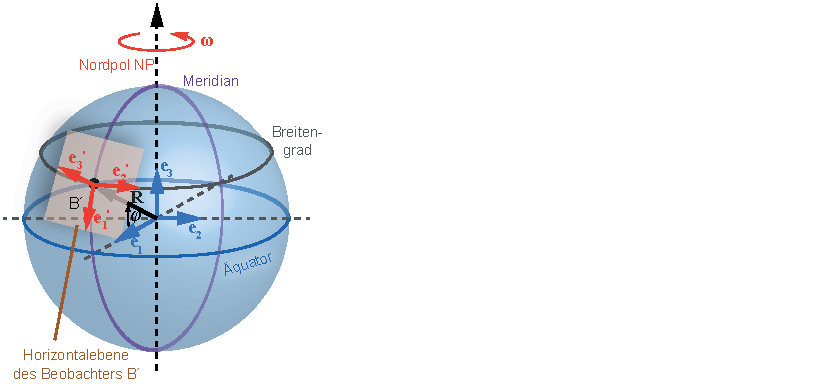
\includegraphics[scale=1]{Rot_Erde_1.pdf}
\caption[Inertialsystems und Nichtinertialsystem der rotierenden Erde.] {Darstellung des Inertialsystems $\vec{\Sigma} = (\veceX,\veceY,\veceZ) = (\vecez,\vecey,\vecez)$, in dem sich die Erde dreht. Das Nichtinertialsystem $\vec{\Sigma}' = (\vecpeX,\vecpeY,\vecpeZ)=(\vecpex,\vecpey,\vecpez)$ bewegt sich mit einem Beobachter B' auf der Erdoberfl�che mit.}\label{abb:bew_Rot_Erde1}
\end{figure}

\begin{figure}
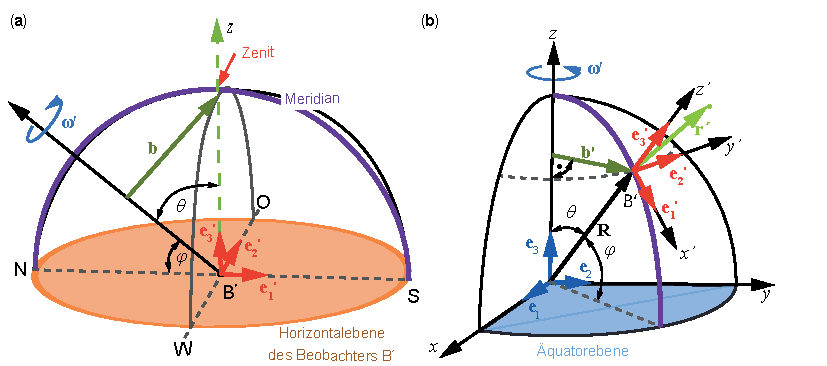
\includegraphics[scale=1]{Rot_Erde_4.pdf}
\caption[Bezugssysteme f�r die Behandlung der Erdrotation.]{Bezugssysteme f�r die Behandlung der Erdrotation. \fa Nichtinertialsystem, das sich mit einem Beobachter B' auf der Erdoberfl�che mitbewegt. Darstellung der beiden Bezugssysteme $\vec{\Sigma} = (\veceX,\veceY,\veceZ) = (\vecez,\vecey,\vecez)$ (Erde ruhend) und $\vec{\Sigma}' = (\vecpeX,\vecpeY,\vecpeZ)=(\vecpex,\vecpey,\vecpez)$. \fb Mitrotierender Beobachter auf der Erdoberfl�che.}\label{abb:bew_Rot_Erde4}
\end{figure}

Wir w�hlen das kartesische Inertialsystem $\vec{\Sigma}$ so, dass in dessen Ursprung der Mittelpunkt der rotierenden Erde liegt.
Das mitbewegte ebenfalls kartesische 
KOS $\vec{\Sigma} '$ sei mit einem beliebig w�hlbaren, aber festen Beobachterpunkt B' auf der Oberfl�che der Erde verbunden, der den Ursprung von $\vec{\Sigma} '$ bildet.
Somit rotiert das KOS $\vec{\Sigma} '$ zusammen mit dem Punkt B' relativ zu $\vec{\Sigma}$.
Die Erdrotation wird in $\vec{\Sigma}$ durch die Winkelgeschwindigkeit $\omega$ beschrieben, die f�r die Erde $2\pi/86164 \SI{}{\per\second} = \SI{7.292e-5}{\per\second}$ betr�gt.%
\footnote{Man beachte, dass man hier f�r die Erdumdrehung den siderischen Tag nehmen muss. In vielen Literaturstellen wird $\omega$ irrt�mlich mit $2\pi/86400 \SI{}{\per\second}$ angegeben, was der Dauer eines Sonnentages entspricht. Der Unterschied ist gering, aber nachweisbar, siehe auch Kapitel 3.1.2 in Himmelsmechanik (Band II, Kapitel 3).}
Wir w�hlen $\vec{\Sigma}'$ nun so, dass die $\vecpeZ$-Achse senkrecht von der Erdoberfl�che in den Himmel zeigt und die $\vecpeX$-Achse nach S�den.
Dann zeigt die $\vecpeY$-Achse nach Osten.

Bevor wir die verschiedenen Probleme und �bungen in Angriff nehmen, m�ssen wir etwas zum Vektor $\vec{\omega}'$ und zum Vektor $\vec{R}'$ erl�utern, da es hier immer wieder zu Problemen mit Vorzeichen und Zuordnung kommt.
Beide Vektoren m�ssen in den Basisvektoren von $\vec{\Sigma} '$, also den ${\vec{e}_i}'$, ausgedr�ckt werden.
Aus \figref{bew_Rot_Erde4} liest man ab:
\begin{align}
    \vec{\omega}' &= - \omega \cos{\varphi}\: \vecpeX + \omega \sin{\varphi}\: \vecpeZ\:=\: \omega\: \begin{pmatrix} -\cos{\varphi} \\ 0 \\ \sin{\varphi} \end{pmatrix} = \vec{\omega}'_{\|}  + \vec{\omega}'_{\bot} ~~~ \text{mit} \nonumber \\
    \vec{\omega}'_{\|} &= \begin{pmatrix} -\omega \cos{\varphi} \\ 0 \\ 0 \end{pmatrix} ~~\:\text{und}\:~~ \vec{\omega}'_{\bot}  = \begin{pmatrix} 0 \\ 0 \\ \omega \sin{\varphi} \end{pmatrix}~. \label{eq:bew_Omega_Ko}
\end{align} 
Der Winkel $\varphi$ wird dabei, wie in \figref{bew_Rot_Erde4} gezeigt, im System $\vec{\Sigma}$ gemessen.
F�r den Vektor $\vec{R}'$ gilt  $\vec{R}' = -R \:\vecpeZ$, da der Verschiebungsvektor im gestrichenen System vom Beobachter B' zum Erdmittelpunkt (Ursprung von $\vec\Sigma$) zeigt.
F�r die Erdoberfl�che gelten folgende Parameter:\\
\begin{align*}
	\dot{\vec{\omega}}' &= 0 ~,~~  \ddot{\vec{R}}' = 0 ~,~~  \dot{\vec{R}}' = 0 ~~,~ \vec{r} = \vec{R}'  + \vec{r}'\,,~\\ \text{und wegen } ~~\left|\vec{r}'\right| &\ll \min(\left|\vec{R}\right|, ~\left|\vec{r}\right|)~ \text{folgt}~~	\left|\vec{r}\right| \approx \left|\vec{R}\right|~.
\end{align*}
Wir starten von \eqref{eq:bew_Rot_System2} und erhalten mit   \eqref{eq:bew_Coriolis_Kraft} , \eqref{eq:bew_Zentrifugal_Kraft} und der Erdmasse $M_\text{E}$:
\begin{align}
	m\:\ddot{\vec{r}}'\;&= \;\vec{F_\text{G}} + \vec{F'_\text{Z}} + \vec{F'_\text{Cor}} \nonumber \\
	\Rightarrow \ddot{\vec{r}}'\;&= \;-\frac{G M_\text{E}}{r^3} \vec{r} - \underbrace{\vec{\omega}' \times \lk \vec{\omega}' \times  \vec{r}' \rk}_{\approx 0}  + \underbrace{\vec{\omega}' \times \lk \vec{\omega}' \times  \vec{R}' \rk}_{\vec{\omega}'(\vec{\omega}'\cdot\vec{R}') - \vec{R}'(\vec{\omega}'\cdot\vec{\omega}')}\: \: \underbrace{- 2 \vec{\omega}' \times \dot{\vec{r}}'}_{\vec{F}'_\text{Cor}/m} \nonumber \\
	\Rightarrow \ddot{\vec{r}}'\;&= \;- g_0 \:\vecpeZ \: + \: \underbrace{R \omega ^2 \lk\vecpeZ-\frac{\vec{\omega}'}{\omega ^2} (\vec{\omega}'\cdot \vecpeZ) \rk}_{\vec{b}'} \:- \:2 \vec{\omega}' \times \dot{\vec{r}}' \nonumber \\
	\Rightarrow \ddot{\vec{r}}'\;&= \;- \underbrace{\lk g_0 \:\vecpeZ \: - \: \vec{b}' \rk}_{\vec{g}'} \: \underbrace{-\: 2 \vec{\omega}' \times \dot{\vec{r}}'}_{\vec{F}'_\text{Cor}/m} ~.  \label{eq:bew_BGL_Erdrotation}
\end{align}
Mit \eqref{eq:bew_BGL_Erdrotation} haben wir die Bewegungsgleichungen f�r einen erdoberfl�chennahen K�rper im mitbewegten KOS auf der Erdoberfl�che gefunden.
Der Vektor $\vec{b}'$ ist ein Differenzvektor von $\vec{\omega}'$ und $\vecpeZ$ und ist auch in \figref{bew_Rot_Erde4} und \figref{bew_Rot_Erde5} eingezeichnet.
Er steht immer senkrecht auf $\vec{\omega}'$ und seine Komponenten k�nnen mit \eqref{eq:bew_Omega_Ko} zu 
\begin{align*}
    \vec{b}' &= R \omega^2 \lek \begin{pmatrix} 0 \\ 0 \\ 1 \end{pmatrix} - \begin{pmatrix} -\cos{\varphi}\cdot \sin{\varphi} \\ 0 \\ (\sin{\varphi})^2  \end{pmatrix}\rek \nonumber = R \omega^2 \lek \begin{pmatrix} + \frac{1}{2}\sin{2 \varphi} \\ 0 \\ 0  \end{pmatrix} + \begin{pmatrix} 0 \\ 0 \\ (\cos{\varphi})^2  \end{pmatrix} \rek \;=\;\:\vec{b}'_{\|} + \vec{b}'_{\bot} 
\end{align*}
berechnet werden.
Betrag und Richtung von $\vec{b}'$ sind damit abh�ngig von der geographischen Breite $\varphi$. 
Den Zusatzterm $\vec{b}'_{\bot}$ in radialer Richtung $\vecpeZ$ k�nnen wir mit der Schwerebeschleunigung $g_0 \cdot \vecpeZ$ zu einer effektiven Schwerebeschleunigung $\vec{g}_\text{eff}$ mit dem Betrag 
\begin{align}
	\vec{g}_\text{eff} \:=\: g_\text{eff} \,\vecpeZ \:= \:g_0 \,\vecpeZ - \vec{b}'_{\bot} \: =\: \lk \:g_0 -\: R \omega^2 (\cos{\varphi})^2\rk \vecpeZ\, \label{eq:bew_effektives_g}
\end{align} 
zusammenfassen.
Der tangentiale Zusatzterm $\vec{b}'_{\|}$ in S�d-Richtung $\vecpeX$ ist f�r $\varphi = 45\degree$ maximal und verschwindet an den Polen und am �quator.
Eine Folge dieser Kraftkomponente ist die Abplattung der Erde, denn die fr�her fl�ssige Erde stellte sich mit der Zeit so ein, dass die Oberfl�che senkrecht zur Resultierenden aus $\vec{g}_0$ und $\vec{b}'_{\|}$ liegt, also senkrecht zu $\vec{g}'$.\footnote{Man beachte, dass  $\vec{g}'$ nicht mehr zum Erdmittelpunkt zeigt (\probref{bew_AbplattungPlaneten}).}
Als Folge dieser Abplattung kommt es zu einer weiteren Abnahme der Schwerebeschleunigung am �quator �ber Gl. \eqref{eq:bew_effektives_g} hinaus, in welcher wir ja eine kugelf�rmige Erde angenommen hatten. Formel \eqref{eq:bew_effektives_g} bleibt dennoch eine gute N�herung.

\begin{figure}
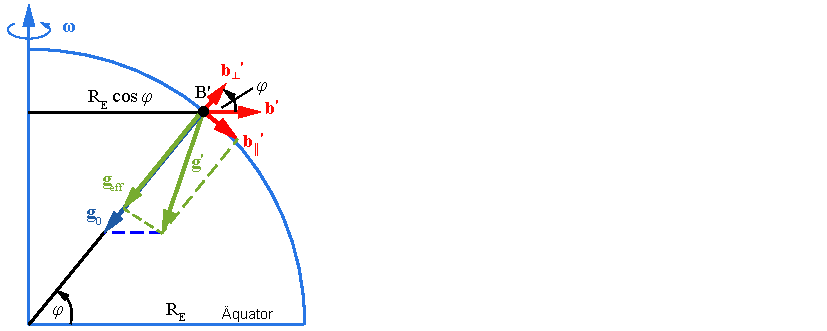
\includegraphics[scale=1]{Rot_Erde_5.pdf}
\caption[Abh�ngigkeit der Schwerebeschleunigung von der geographischen Breite.] {Abh�ngigkeit der Schwerebeschleunigung von der geographischen Breite $\varphi$. Zur Deutlichkeit sind die L�ngenverh�ltnisse stark �bertrieben. Man mache sich klar, dass $\left| \vec{b}' \right| \approx 0.05 \,g$ ist. Ebenso m�ge der Leser das Bild f�r die s�dliche Hemisph�re zeichnen, um zu erkennen, dass wegen der $\sin{\varphi}$-Abh�ngigkeit die Komponente $\vec{b}'_{\|}$ nach Norden zeigt.}
\label{abb:bew_Rot_Erde5}
\end{figure}

Wir wenden uns jetzt dem Term der Coriolis-Kraft $\vec{F'_\text{Cor}}$ zu.
Wegen \eqref{eq:bew_Omega_Ko} und $\dot{\vec{R}}'= 0 $ kann diese in zwei Komponenten zerlegt werden:
\begin{align}
	\vec{F'_\text{Cor}} = - 2 m \lek \lk \vec{\omega}'_{\bot}  \times \dot{\vec{r}}' \rk + \lk \vec{\omega}'_{\|} \times  \dot{\vec{r}}' \rk \rek ~. \label{eq:bew_Coriolis_Ko}
\end{align} 
Der Term mit $\vec{\omega}'_{\bot}$ f�hrt bei einer Bewegung auf der Erdoberfl�che zu einer seitlichen Ablenkung, w�hrend der Term mit $\vec{\omega}'_{\|}$ zu einer vertikal (aufw�rts oder abw�rts) gerichteten Kraft f�hrt.
Die seitlich gerichtete Kraft ist von gro�er Bedeutung f�r Zyklone, Meeresstr�mungen und die Ballistik (\probref{bew_Coriolis_I}--\probref{bew_Coriolis_III}).
Um die Effekte, die durch die Coriolis-Kraft im mitbewegten System auftreten, besser berechnen und verstehen zu k�nnen, schreiben wir \eqref{eq:bew_BGL_Erdrotation} in den einzelnen Komponenten:
\begin{align}
    \begin{pmatrix} \ddot{x}' \\  \ddot{y}' \\  \ddot{z}' \end{pmatrix} \:=\: - 2 \omega \: \begin{pmatrix} -\frac{1}{4} R \omega \sin{2\varphi} - \dot{y}' \sin{\varphi} \\ \dot{x}' \sin{\varphi} + \dot{z}' \cos{\varphi} \\ -\dot{y}' \cos{\varphi} + g_\text{eff}/(2 \omega) \end{pmatrix} ~. \label{eq:bew_BGL_Erdrotation_Ko}
\end{align}
Wir haben mit \eqref{eq:bew_BGL_Erdrotation_Ko} ein System dreier gekoppelter Differentialgleichungen als Bewegungsgleichungen f�r Massepunkte im mitbewegten System gewonnen.
Diese Gleichungen k�nnen numerisch f�r verschiedene Anfangsbedingungen gel�st werden (\probref{bew_Coriolis_I}).
Um eine N�herungsl�sung f�r $\omega \,t \ll 1$ (was bei den betrachteten Bewegungen nahe der Erdoberfl�che erf�llt ist) angeben zu k�nnen, mit der man die wesentlichen Effekte erkennen kann, vernachl�ssigen wir alle Terme mit $\omega^2$.
Einmalige Integration von \eqref{eq:bew_BGL_Erdrotation_Ko} ergibt:
\begin{align}
    \begin{pmatrix} \dot{x}' \\  \dot{y}' \\  \dot{z}' \end{pmatrix}\:=\: \: \begin{pmatrix} 2 \omega y' \sin{\varphi} + C_x\\ - 2 \omega\ \lk x' \sin{\varphi} + z' \cos{\varphi} \rk + C_y \\ 2 \omega y' \cos{\varphi} - g_\text{eff}\,t + C_z \end{pmatrix}~. \label{eq:bew_BGL_Erdrotation_Approx1}
\end{align}
F�r den \emph{freien Fall} \index{Fall!freier} ergeben sich aus den Anfangsbedingungen
	\[x'(0) =\: y'(0) =\: \dot{x}'(0) =\: \dot{y}'(0) =\: \dot{z}'(0) =\: 0 \quad \text{und} \quad z'(0) =\: h 
\]
die Integrationskonstanten zu $C_x = C_z = 0$ und $C_y = 2 \omega h \cos{\varphi}$. 
In \eqref{eq:bew_BGL_Erdrotation_Approx1} kann man wiederum alle Terme mit $ \omega x'$ und $\omega y'$ vernachl�ssigen, da $x'$ und $y'$ selbst proportional zu $\omega$ sind, woraus n�herungsweise
\begin{align}
    \begin{pmatrix} \dot{x}' \\  \dot{y}' \\  \dot{z}' \end{pmatrix}\: \approx \: \begin{pmatrix} 0 \\ 2 \omega \lk h -  z' \rk \cos{\varphi} \\ - g_\text{eff}\,t \end{pmatrix} \label{eq:bew_BGL_Erdrotation_Approx2}
\end{align}
folgt. 
Mit $g_\text{eff} \approx g$ folgt f�r die $z'$-Komponente die bekannte L�sung f�r den freien Fall und f�r die beiden anderen Komponenten durch Einsetzen der L�sung f�r $z'(t)$ und unter Ber�cksichtigung der Anfangsbedingungen schlie�lich als N�herungsl�sung
\begin{align}
    \begin{pmatrix} x'(t) \\ y'(t) \\ z'(t) \end{pmatrix}\:=\: \: \begin{pmatrix} 0 \\ \omega\ g \frac{t^3}{3} \cos{\varphi} \\ h - g \frac{t^2}{2} \end{pmatrix}~. \label{eq:bew_BGL_Erdrotation_Lsg1}
\end{align}
F�r eine Fallzeit $t_f = \sqrt{\frac{2h}{g}}$ (aus $z'(t_f) = 0$) ergibt sich f�r die interessante $y'$-Komponente 
\begin{align}
	y'_f = \frac{2 \omega h \cos{\varphi}}{3} \sqrt{\frac{2h}{g}} ~.\label{eq:bew_BGL_Erdrotation_Lsg2}
\end{align}
F�r einen frei fallenden K�rper kommt es also zu einer Ostablenkung, die am �quator am gr��ten ist.
Man kann sich leicht �berlegen, dass die Coriolis-Kraft auf andere ballistische und Bewegungsph�nomene auf der Erde einen nicht zu vernachl�ssigenden Einfluss hat.
Gleichungssystem \eqref{eq:bew_BGL_Erdrotation_Ko} gibt uns die Grundlage daf�r, einige dieser Effekte,
die ein Beobachter auf der Erdoberfl�che \anf{sieht},
wie \zb Projektilabweichungen und Zyklonrichtungen\index{Zyklon}%
\footnote{Ein Zyklon ist ein tropischer Wirbelsturm im indischen und s�dlichen pazifischen Ozean.
Dagegen werden mit Hurrikans Wirbelst�rme bezeichnet, die an den K�sten des amerikanischen Doppelkontinents auftreten.
Wirbelst�rme in Ost- und S�dostasien hingegen werden Taifune genannt.
Wir benutzen Zyklone als �berbegriff.} erkl�ren und berechnen zu k�nnen (\probref{bew_Coriolis_III}).

\subsection{Oszillatoren und Pendel}\index{Pendel} \label{kap:bew_pendulum}

Wir hatten uns bereits in \kap{bew_schwingung} auf der Basis des Lagrange-Formalismus mit den grundlegenden Bewegungsgleichungen f�r schwingende Systeme besch�ftigt.
Wie dort erl�utert, findet man solche Systeme an vielen Stellen in der Natur und damit auch in der Physik.
Wir wollen das Thema deswegen in diesem Kapitel mit einigen konkreten Beispielen vertiefen.  
Wir werden dabei die Vielfalt der schwingenden Systeme kennenlernen und uns dar�ber hinaus auch mit den Ph�nomenen der Reibung, der Resonanz und der nichtlinearen Kopplung besch�ftigen.
Letztere liefern uns eine Reihe von \zt �berraschenden Effekten bis hin zu chaotischem Verhalten.
Es ist auch erstaunlich, wie viele ber�hmte Physiker sich �ber die Jahrhunderte hinweg mit der Theorie schwingender Systeme, insbesondere mit Pendelproblemen, besch�ftigt haben.
Das Pendel hat �ber lange Zeit hinweg eine wesentliche Rolle bei der Zeitmessung gespielt. 
Auch Philosophen und K�nstler wurden vielfach von den Schwingungen des Pendels inspiriert.
Wir empfehlen dem interessierten Leser, in der sehr sch�nen und umfangreichen Zusammenfassung zur Physik, Geschichte und Kunst rund um das Pendel in \cite{Matthews2005} zu lesen.

\subsubsection{Der harmonische Oszillator} \index{Oszillator!harmonischer|textbf} \label{kap:bew_harmon_oszillator}

Wir beginnen mit dem harmonischen Oszillator, dessen Bewegungsgleichung wir bereits in \kap{bew_schwingung} als Grenzfall f�r kleine Schwingungen hergeleitet hatten, siehe Gleichung \eqref{eq:bew_Schwingung01a}. 
Die Lagrange-Funktion\index{Lagrange-Funktio} des eindimensionalen harmonischen Oszillators hatten wir bereits in den Kapiteln \ref{kap:bew_Lagrange_II} und \ref{kap:bew_Lagrange_II_R} aufgestellt:
\begin{align}
	\mathcal{L} = \frac{1}{2} m \,\dot{q}^2 \,-\,\frac{1}{2} k\,q^2 \,. \label{eq:bew_pendulum01}
\end{align}
Wir k�nnen daraus die Bewegungsgleichung f�r die verallgemeinerte Koordinate $q$ ableiten, indem wir die Lagrange-Funktion um einen Reibungsterm und eine zeitlich variierende externe Kraft erweitern. 
Wir erhalten
\begin{align}
	\ddot{q} + \eta_n \,\dot{q}^n + {\omega_0}^2 \, q \,=\, \frac{F^{\text{\,(ext)}}(t)}{m} = \frac{F_\text{A}\,\cos(\omega_\text{A}t + \delta_\text{A})}{m}\label{eq:bew_pendulum02}
\end{align}
mit ${\omega_0}^2 = k/m$ und einem Reibungskoeffizienten $\eta_n$, wobei $n$ entweder $1$ oder $2$ ist.
Hierbei haben wir eine (verallgemeinerte) externe Kraft $F^{\text{ext}}(t)$ als harmonische Schwingung mit einer Anregungsfrequenz $\omega_\text{A}$ und einer Amplitude von $F_\text{A}$ angenommen.
Wir behandeln den Fall $n=1$.
Dann ist \eqref{eq:bew_pendulum02} eine lineare inhomogene Differentialgleichung (DGL), in der wir, um etwas Schreibarbeit zu sparen, $\eta_1 = 2 \gamma$ setzen.
Dann erhalten wir mit dem gleichen Ansatz $Q = Q_0 \mathrm{e}^{\mathrm{i}\omega t}$ wie in \eqref{eq:bew_Schwingung03} f�r die homogene DGL die Bestimmungsgleichung
\begin{align*}
	\lk -\omega^2 + 2\gamma \, \mathrm{i} \,\omega + {\omega_0}^2 \rk \, \mathrm{e}^{\mathrm{i} \omega t} = 0\,,
\end{align*}
woraus sich die Schwingungsfrequenz wie folgt ergibt:
\begin{align}
	\omega = \mathrm{i} \, \gamma \pm \sqrt{{\omega_0}^2 - \gamma^2} = \mathrm{i} \, \gamma \pm \hat{\omega}~. \label{eq:bew_pendulum03}
\end{align}
Je nach Verh�ltnis von $\omega_0$ und $\gamma$ k�nnen wir die folgenden drei F�lle unterscheiden:
\begin{enumerate} [a) ]
	\item \textit{Schwache D�mpfung, bei} $\omega_0 > \gamma$\\
	Die allgemeine L�sung ist mit einem rellen $\hat{\omega}$ gegeben durch
	\begin{align}
		q(t) = A \mathrm{e}^{-\gamma t}  \sin(\hat{\omega}\,t + \phi) \,, \label{eq:bew_pendulum04}
	\end{align}
	worin $A$ und $\phi$ durch die Anfangsbedingungen gegeben sind.
        Man erkennt, dass die Frequenz $\omega$ des schwach ged�mpften Oszillators leicht zu niedrigeren Frequenzen gegen�ber der Eigenfrequenz $\omega_0$ verschoben ist.
	\item \textit{Starke D�mpfung, bei} $\omega_0 < \gamma$\\
	Hier ist die allgemeine L�sung mit einem rein imagin�ren $\hat{\omega}$, gegeben durch
	\begin{align}
		q(t) = A \mathrm{e}^{-\gamma_1 t} + B \mathrm{e}^{-\gamma_2 t} \,, \label{eq:bew_pendulum05}
	\end{align}
	mit
		\[\gamma_{1,2} = \gamma \pm \sqrt{\gamma^2 - {\omega_0}^2} = \gamma \pm \mathrm{i}\, \hat{\omega} \,.
	\]
	$A$ und $B$ werden wieder durch die Anfangsbedingungen bestimmt.
        Man erkennt, dass es beim stark ged�mpften Oszillator keine Schwingungen gibt.
	\item \textit{Kritische D�mpfung -- aperiodischer Grenzfall, bei} $\omega_0 = \gamma$\\
	Hier ist die allgemeine L�sung durch
	\begin{align}
		q(t) = \lk A + B\, t \rk \mathrm{e}^{-\gamma t} \label{eq:bew_pendulum06}
	\end{align}
gegeben.\footnote{Man beachte, dass man nicht einfach in \eqref{eq:bew_pendulum04} $\gamma_1=\gamma_2$ setzen kann, da wir wegen der DGL zweiter Ordnung zwei linear unabh�ngige L�sungen brauchen.
Siehe dazu auch \cite{Riley2006} und \cite{Otto2019, Fischer2018}.
Man kann aber L�sung \eqref{eq:bew_pendulum06} �ber eine Grenzfallbetrachtung aus \eqref{eq:bew_pendulum04} herleiten.}
Man erkennt aus \figref{bew_HarmonOszillator01}, dass der aperiodische Grenzfall die schnell\-ste D�mpfung des schwingenden Systems ergibt.
$A$ und $B$ werden wieder durch die Anfangsbedingungen bestimmt. 
\end{enumerate}
Um die DGL f�r eine erzwungene Schwingung zu l�sen, muss man eine spezielle L�sung der inhomogenen DGL zur allgemeinen L�sung der homogenen DGL addieren.
Auch dazu machen wir wieder den Ansatz $Q_\text{p} = Q_\text{p0} \, \mathrm{e}^{\mathrm{i}\omega t}$ und erhalten als Bestimmungsgleichung
\begin{align}
	 Q_\text{p0} = \frac{F_\text{A}}{m} \frac{1}{{\omega_0}^2-{\omega_\text{A}}^2 + 2\,\mathrm{i} \,\gamma \omega_\text{A}}\,.\label{eq:bew_pendulum07}  
\end{align}

Da im Allgemeinen $\gamma \neq 0$ gilt, ist $Q_\text{p0}$ eine komplexe Zahl, die wir als
\begin{align*}
	Q_\text{p0} = \Re \, Q_\text{p0} + \im\,\Im \, Q_\text{p0}
\end{align*}
darstellen k�nnen mit
\begin{align}
 	\Re \, Q_\text{p0} &= \frac{F_\text{A}}{m} \frac{({\omega_0}^2 - {\omega_\text{A}}^2)}{( {\omega_0}^2 - {\omega_\text{A}}^2)^2 + 4 \gamma^2 \,{\omega_\text{A}}^2 }\,,
 	\label{eq:bew_pendulum08} \\
 	\Im \, Q_\text{p0} &= - \frac{F_\text{A}}{m} \frac{2 \omega_\text{A}\, \gamma}{( {\omega_0}^2 - {\omega_\text{A}}^2)^2 + 4 \gamma^2 \,{\omega_\text{A}}^2 } \,. \label{eq:bew_pendulum09}
 \end{align} 
Wir k�nnen daraus die allgemeine L�sung der inhomogenen DGL f�r $q(t)$ herleiten:
\begin{align}
	q(t) = A(\omega_\text{A}) \cos(\omega_\text{A}t - \varphi(\omega_\text{A})) 
		+ \hat{A} \mathrm{e}^{- \gamma t} \cos \lk \hat{\omega}t - \hat{\delta}\rk
		\label{eq:bew_pendulum10}
\end{align}
mit
\begin{align*}
	A(\omega_\text{A}) &= \frac{F_\text{A}}{m} \frac{1}{\sqrt{({\omega_0}^2 - {\omega_\text{A}}^2)^2 + 4 \gamma^2 \, {\omega_\text{A}}^2}} \\
	\varphi(\omega_\text{A}) &= - \frac{\Im \, Q_\text{p0}}{\Re \, Q_\text{p0}} 
	= \arctan \lk \frac{2 \gamma \,\omega_0}{{\omega_0}^2 - {\omega_\text{A}}^2} \rk \\
 \hat{\omega} &= \sqrt{{\omega_0}^2 - \gamma^2} \,. 
\end{align*}
Die Parameter $\hat{A}$ und $\hat{\delta}$ bestimmen sich wieder aus den Anfangsbedingungen.
Man erkennt folgendes:
\begin{itemize}
	\item F�r $t \gg 1/\gamma$ bleibt nur die spezielle L�sung �brig, \dh nach dem Einschwingen schwingt der Oszillator mit der Frequenz $\omega_\text{A}$.
	\item W�hrend des Einschwingens kann es zu Schwebungen zwischen $\omega_0$ und $\omega_\text{A}$ kommen.
          Diese dauern umso l�nger, je geringer die D�mpfung ist.
	\item Amplitude $A(\omega_\text{A})$ und Phasenlage $\varphi(\omega_\text{A})$ h�ngen von der Anregungsfrequenz $\omega_\text{A}$ ab. 
	Die Resonanzfrequenz der Amplitude ist gegeben durch
	\[\omega_\text{max} = \sqrt{{\omega_0}^2 - 2\gamma^2}~\] und ergibt eine maximale Amplitude von 	
		\[A_\text{max}(\omega_\text{max}) = \frac{F_\text{A}}{m}\frac{1}{2\gamma \sqrt{{\omega_0}^2-\gamma^2}}\,.
	\]
	\item Die Halbwertsbreite der Resonanz ist durch
	\[ \delta_\omega = \omega_+ - \omega_-  
	\qquad \text{mit} \qquad 
	{\omega_\pm}^2 = {\omega_0}^2 - 2 \gamma^2 \pm 2 \gamma \sqrt{{\omega_0}^2 - \gamma^2}\]
	gegeben.
	Man erkennt, dass die Halbwertsbreite gr��er ist, je gr��er die D�mpfung ist.\footnote{Die Halbwertsbreite wird �ber die Gr��e $(A(\omega_\text{A}))^2$ bestimmt, da man \ia als Messgr��e die Intensit�t verwendet, welche proportional zum Quadrat der Amplitude $A$ ist.}
	\item F�r $\gamma \ll \omega_0$ gehen die Beziehungen �ber in
		\begin{align*}
			A_\text{max} &= \frac{F_\text{A}}{m} \frac{1}{2 \gamma\, \omega_0} \,,\\
			\omega_\text{max} &= \omega_0 - \frac{\gamma^2}{\omega_0} \approx \omega_0 \,,\\
			\delta_\omega &= 2 \gamma \,.
		\end{align*}
\end{itemize}
Wir m�chten an dieser Stelle darauf hinweisen, dass wir bei unseren Rechnungen immer noch kleine Auslenkungen $q$ angenommen haben.
Das mag aber insbesondere im Resonanzfall nicht immer erf�llt sein, weswegen man dann zur exakten L�sung �bergehen muss.
Diese werden wir im n�chsten Kapitel behandeln.

Zuvor wollen wir noch die Leistungs�bertragung von der Anregungsquelle auf den Oszillator betrachten.
Da das System nicht konservativ ist, gibt es eine Verlustleistung der Anregungsquelle.
Diese ist gegeben durch
\[  P_\text{V} = - \eta_1 \,m \,\dot{q}\,\dot{q} = -2 \gamma\,m \,\dot{q}^2 \]
\bzw zeitlich gemittelt
\begin{align}
	\left\langle P_\text{V} \right\rangle  &= \frac{1}{T} \int_0^T P_\text{V}(t') \, \D t' = -2 \gamma m \lek A(\omega_\text{A})\rek^2 {\omega_\text{A}}^2 \left\langle \sin^2(\omega_\text{A}t - \delta_\text{A}) \right\rangle \nonumber \\
	&= - \gamma m \lek A(\omega_\text{A})\rek^2  {\omega_\text{A}}^2 \, , \label{eq:bew_pendulum12}
\end{align}
weil \[ \bigintssss_0^{T=\frac{2 \pi}{\omega_\text{A}}} \sin^2(\omega_\text{A}t' - \delta_\text{A}) \, \mathrm{d}t' = \frac{1}{2}\] ist. 
Man erkennt auch, dass die Verlustleistung bei Resonanz am gr��ten ist, \dh dass in diesem Fall die meiste Energie von der Quelle auf den Oszillator �bergeht.  

Im \mscr{} \mlbewref{HarmonOszillator.m} sind die Rechnungen im Detail ausgef�hrt und einige Diagramme daraus bereits in \figref{bew_HarmonOszillator01} und \figref{bew_HarmonOszillator02} gezeigt.
Wir weisen darauf hin, dass $\eta_1$ bzw. $\gamma$ dieselbe Einheit besitzen wie $\omega_0$, also $\si{s^{-1}}$.
Darum kann $1/\gamma$ als die Zeitspanne interpretiert werden, nach der die Oszillation stark abgeklungen ist.
In \probRef{bew_HO_quadrat} wird auch der Fall f�r eine quadratisch von der Geschwindigkeit abh�ngende Reibung numerisch behandelt.
Reibungskr�fte, die quadratisch in $\dot{q}$ sind, machen die mathematische Behandlung wesentlich komplizierter, da die Bewegungsgleichung dann nichtlinear ist.
Wir geben in der L�sung zu \probref{bew_HO_quadrat} auch die weiterf�hrende Literatur \cite{Smith2012} zur analytischen Behandlung dieser nichtlinearen DGL an und vergleichen die analytische mit unserer numerischen L�sung.

\begin{figure}
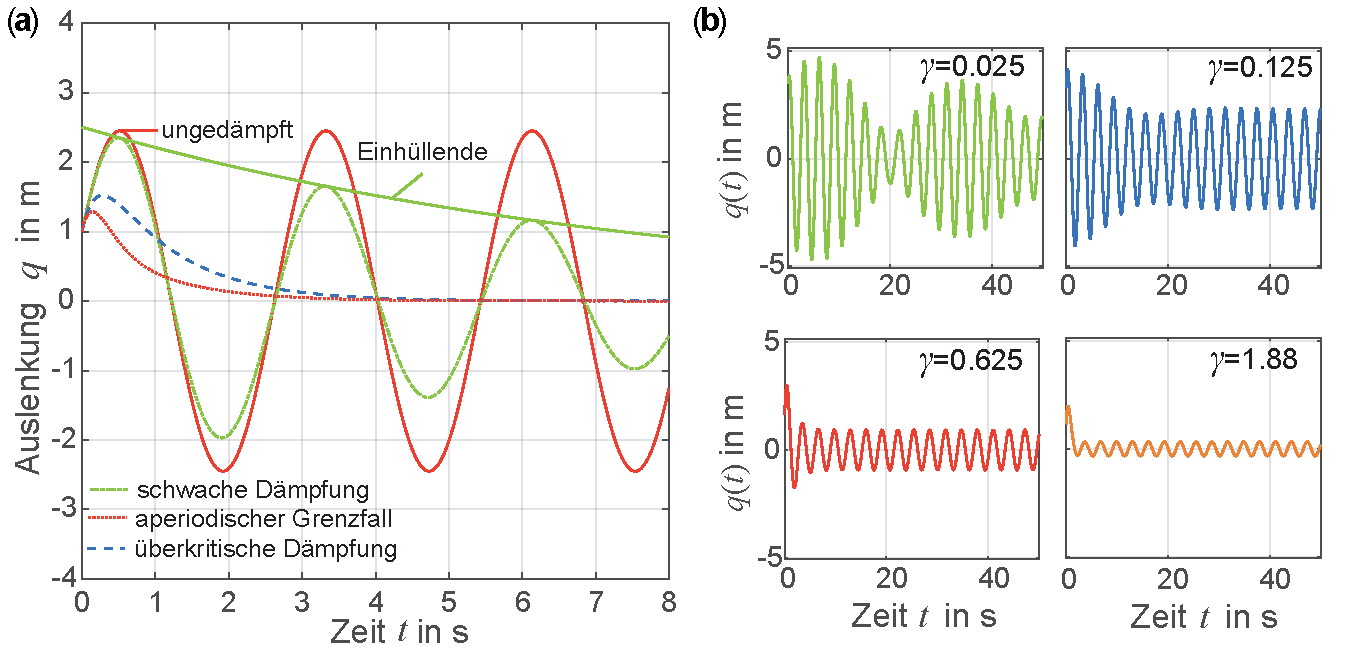
\includegraphics[width=\textwidth]{HarmonOszillator01.pdf}
\caption[D�mpfung des harmonischen Oszillators und Einschwingverhalten.] {\fa D�mpfung des harmonischen Oszillators und \fb dessen Einschwingverhalten f�r verschiedene Reibungskoeffizienten $\gamma$ und $\omega_0/\omega_\text{A}=0.9$.} 
\label{abb:bew_HarmonOszillator01}
\end{figure}

\begin{figure}
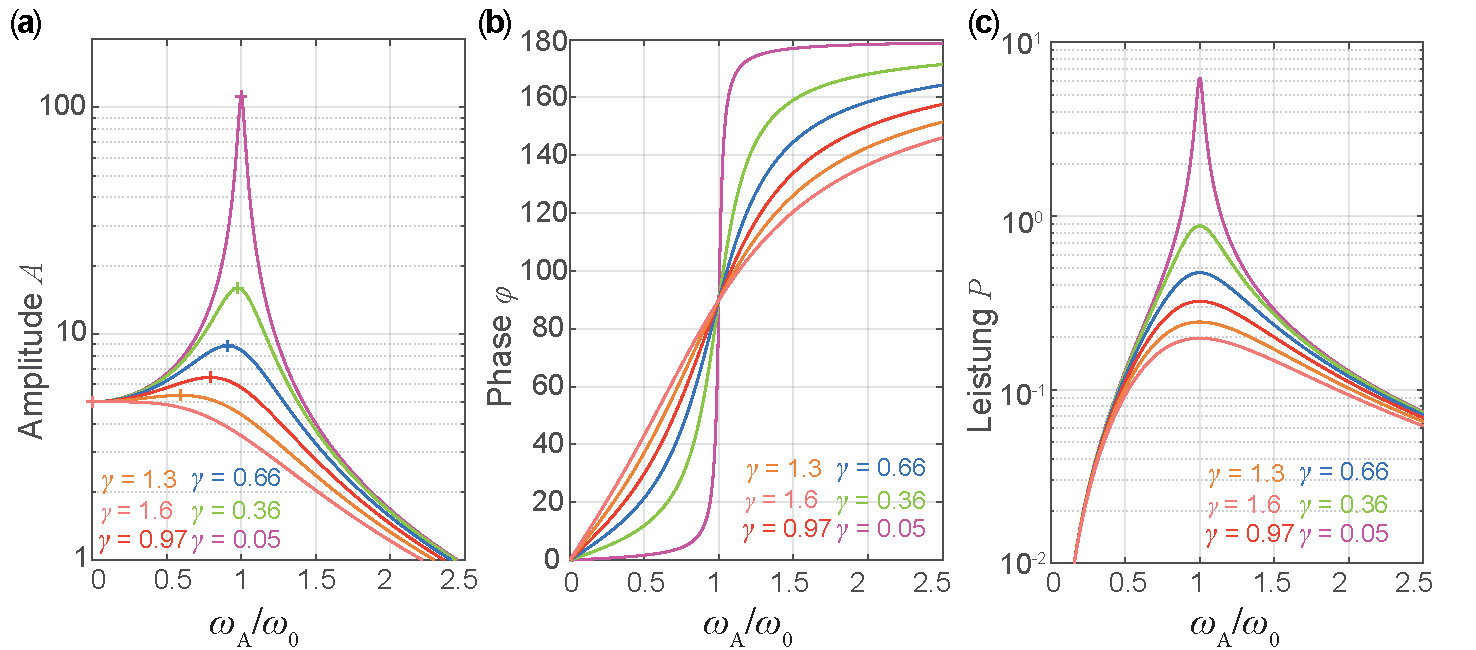
\includegraphics[width=\textwidth]{HarmonOszillator02.pdf}
\caption[Amplitude, Phase und Leistungs�bertragung eines Oszillators.] {\fa Amplitude, \fb Phasen und \fc Leistungs�bertragung beim getriebenen harmonischen Oszillator f�r verschiedene Anregungsfrequenzen und Reibungen.} 
\label{abb:bew_HarmonOszillator02}
\end{figure}

\subsubsection{Der anharmonische Oszillator (Nichtlineares Pendel)} \index{Oszillator!harmonischer} \index{Oszillator!anharmonischer} \index{Pendel!nichtlineares}\index{Pendel!mathematisches}\label{kap:bew_anharmon_oszillator}

Wir haben uns im vorherigen Kapitel auf kleine Schwingungen beschr�nkt, f�r die die Linearisierung \bzw die sogenannte harmonische N�herung galt. 
Wir wollen diese Beschr�nkung jetzt aufgeben und sowohl eine analytische L�sung als auch gut handhabbare N�herungsl�sungen f�r dieses allgemeinere Problem finden. 
Dazu machen wir uns zun�chst noch einmal klar, dass in der linearen N�herung \eqref{eq:bew_pendulum01} die potentielle Energie in der Lagrange-Funktion �berbewertet wird und daher zu erwarten ist, dass in der exakten L�sung des Oszillators die Schwingungsperiode (Eigenfrequenz) von der Amplitude abh�ngig sein wird, und zwar so, dass mit steigender Amplitude auch die Schwingungsperiode zunimmt.
Das erkennt man auch leicht, wenn man in \eqref{eq:bew_Schwingung_d} \bzw \eqref{eq:bew_Schwingung01b} noch den n�chsten Term der Sinus-Entwicklung mitnimmt, der dann wie eine Verringerung der Schwingungskreisfrequenz wirkt.
Die Bewegungsgleichung lautet dann
\begin{align}
                \ddot{\theta}+{\omega_0}^2\, \theta = \frac{{\omega_0}^2\,\theta^3}{6} \ =\kappa_3\,\theta^3 \,. \label{eq:bew_NLOsz01}
\end{align}
F�r einen beliebigen anharmonischen Oszillator gilt ganz allgemein
\begin{align}
                \ddot{x}+{\omega_0}^2 x= \kappa_2\, x^2+\kappa_3 \,x^3 + \ldots = \sum\limits_{j} \kappa_j\,x^j \,.   \label{eq:bew_NLOsz02}
\end{align}

\subparagraph{\textbf{Ansatzmethode zur Berechnung der Schwingungsperiode des nichtlinearen Pendels}}

Wir wollen in unserer Betrachtung auch den Fall einer m�glichen asymmetrischen Schwingung ber�cksichtigen und machen daher den allgemeinen Ansatz
	\begin{align}
			x(t) = A_0 + A_1\cos\omega t + A_2\cos2\omega t + A_3\cos3\omega t \,. \label{eq:bew_NLOsz03}
	\end{align}
Wir setzen diesen Ansatz nun in \eqref{eq:bew_NLOsz02} ein und erhalten f�r die Ableitung auf der linken Seite von \eqref{eq:bew_NLOsz02}
\begin{align}
\ddot{x}  =  - \omega^2 A_1\cos\omega t - 4 \omega^2 A_2\cos2\omega t - 9 \omega^2 A_3\cos3\omega t~. \label{eq:bew_NLOsz03a}
\end{align}
Auf der rechten Seite von \eqref{eq:bew_NLOsz02} ergeben sich dann Terme aus den Potenzen in $x$, bei deren Berechnung wir von verschiedenen trigonometrischen Formeln f�r die Potenzen der Winkelfunkionen Gebrauch machen, insbesondere von  $\cos^2 (\omega t) = (1+ \cos \lk 2 \omega t \rk)/2$ und $\cos^3(\omega t) = (3 \cos \omega t + \cos \lk 3 \omega t \rk)/4$. Wir wollen auch nur die Terme mit Potenzen bis ${A_3}^3$ und Frequenzen bis $3\omega t$ mitnehmen, da wir annehmen wollen, dass $A_2, A_3 \ll A_1$. Es ergeben sich dann folgende Terme:
\begin{align} 
\begin{split}
 \text{f�r}~ x^1 &: A_0 + A_1\cos\omega t + A_2\cos2\omega t + A_3\cos3\omega t \,, \\
 \text{f�r}~ x^2 &: {A_0}^2 + \frac{1}{2} {A_1}^2\cos2\omega t + \frac{1}{2} \lk {A_1}^2 + {A_2}^2 + {A_3}^2 \rk\,, \\
 \text{f�r}~ x^3 &: {A_0}^3 + \frac{3}{4} {A_1}^3\cos\omega t + \frac{3}{4} {A_2}^3\cos2\omega t + \frac{1}{4} \lk {A_1}^3 + 3{A_3}^3 \rk \cos3\omega t \,.
\label{eq:bew_NLOsz04} 
\end{split} 
\end{align}
Wir bringen nun \eqref{eq:bew_NLOsz03a} und \eqref{eq:bew_NLOsz04} zusammen in die Form  
\begin{align}
	T_0 + T_1 A_1 \cos\omega t + T_2 A_2 \cos2\omega t + T_3 A_3 \cos3\omega t = 0   \label{eq:bew_NLOsz05a}
\end{align}
und sortieren nach Argumenten der Winkelfunktionen in die einzelnen Terme $T_i$:
\begin{align} \begin{split}
 \text{f�r}~ \cos 0\omega t &: \qquad  T_0 = A_0 {\omega_0}^2 -\kappa_2 \lk {A_0}^2 + \lk {A_1}^2+{A_2}^2+{A_3}^2 \rk \rk - \kappa_3 {A_0}^3 \,, \\
 \text{f�r}~ \cos 1\omega t &: \qquad  T_1 = - \omega^2 + {\omega_0}^2 - 3 \kappa_3 \frac{{A_1}^2}{4}\,, \\
 \text{f�r}~ \cos 2\omega t &: \qquad  T_2 = A_2 {\omega_0}^2 - 4 A_2 \omega^2 - \kappa_2 \frac{{A_1}^2}{2} - 3 \kappa_3 \frac{{A_2}^3}{4}\,, \\
 \text{f�r}~ \cos 3\omega t &: \qquad  T_3 = A_3 {\omega_0}^2 - 9 A_3 \omega^2 - \frac{\kappa_3}{4} \lk {A_1}^3 + 3 {A_3}^3 \rk \,. \label{eq:bew_NLOsz05} 
\end{split} \end{align}
Damit Bestimmungsgleichung \eqref{eq:bew_NLOsz05a} erf�llt werden kann,
m�ssen alle Terme $T_i$ einzeln verschwinden,
da \eqref{eq:bew_NLOsz05a} f�r alle Zeiten Null sein muss.
Aus $T_1$ in \eqref{eq:bew_NLOsz05} folgt dann sofort $\omega^2 = {\omega_0}^2 - \frac{3\kappa_3}{4} {A_1}^2$ und damit
\begin{equation}
    \omega = \omega_0 \sqrt{1 - \frac{3\,\kappa_3}{\lk 2 \omega_0 \rk^2} {A_1}^2}
    \label{eq:bew_NLOsz06}~,
\end{equation}
was bedeutet, dass die Kreisfrequenz des anharmonischen Oszillators wie erwartet kleiner ist als die des harmonischen Oszillators
und dar�ber hinaus von der Amplitude $A_1$ abh�ngt.
Aus der Bedingung $T_3=0$ folgt dann f�r ${A_3}^3 \approx 0$ (wegen $A_3 \ll A_1$) die Beziehung
\begin{equation}
    A_3 \approx \frac{\kappa_3 {A_1}^3}{27\,\kappa\, {A_1}^2 - 32\, {\omega_0}^2} \label{eq:bew_NLOsz07}~.
\end{equation}
Gehen wir nun speziell zum Fall des \textit{nichtlinearen Pendels} �ber, dann folgt mit $\kappa_2 = 0$ aus den Termen $T_0\,, T_2$ sofort $A_0 =0\,, A_2=0$ und wir k�nnen unsere L�sung aufschreiben als
\begin{equation}
    \theta(t) = \theta_A \, \cos(\omega\,t) + {\theta_A}^3 \lk \frac{1}{27\,{\theta_A}^2-192} \rk \, \cos(3\, \omega\,t) \label{eq:bew_NLOsz08}
\end{equation}
mit der Schwingungsfrequenz \bzw der Schwingungsperiode 
\begin{align} 
\begin{split}
			\omega &= \omega_0 ~ \sqrt{1-\frac{{\theta_\text{A}}^2}{8}}\,,~~T_\text{P} = \frac{T_0}{\sqrt{1-{\theta_\text{A}}^2/8}} \,. \label{eq:bew_NLOsz12}
\end{split}
\end{align}
Wie erwartet wird die Schwingungsperiode mit zunehmender Auslenkung gr��er. In der Literatur \cite{Hinrichsen2021} findet man eine ganze Reihe �hnlicher N�herungen f�r die Schwingungsperiode \eqref{eq:bew_NLOsz12}, die im Allgemeinen auf der Basis verschiedener N�herungen in der Taylor-Entwicklung beruhen. Jakob Bernoulli\indexp{Bernoulli, Jakob}\footnote{Jakob Bernoulli (1655--1705) war ein Schweizer Mathematiker und Physiker, der wesentlich zur Entwicklung der Wahrscheinlichkeitstheorie sowie zur Variationsrechnung und zur Untersuchung von Potenzreihen beigetragen hat.} gab bereits 1749 eine sehr gute N�herung mit 
\begin{equation}
    T_B(\theta_\text{A}) = T_0 \lk 1 + \frac{{\theta_\text{A}}^2}{16}\rk \label{eq:bew_NLOsz09}
\end{equation}
an.
Weitere interessante N�herungen sind 
  \begin{align}
    T_{\text{KF}} = T_0 \frac{1}{\sqrt{\cos \lk \frac{\theta_\text{A}}{2}\rk}} ~~\text{\cite{Hinrichsen2021,Kidd2002} ~~und} ~~
    T_{\text{DE}} = T_0 \frac{1}{1- \frac{{\theta_\text{A}}^2}{16}} ~~\text{\cite{Denman1959}} \,.
  \end{align}
\figref{bew_NLOsz01} vergleicht diese verschiedenen N�herungen (\mscr{} \mlbewref{AnHarmonOszillator01.m}) mit der exakten analytischen Berechnung der Schwingungsperiode �ber das elliptische Integral, die wir im Folgenden vornehmen wollen. 

\begin{figure}
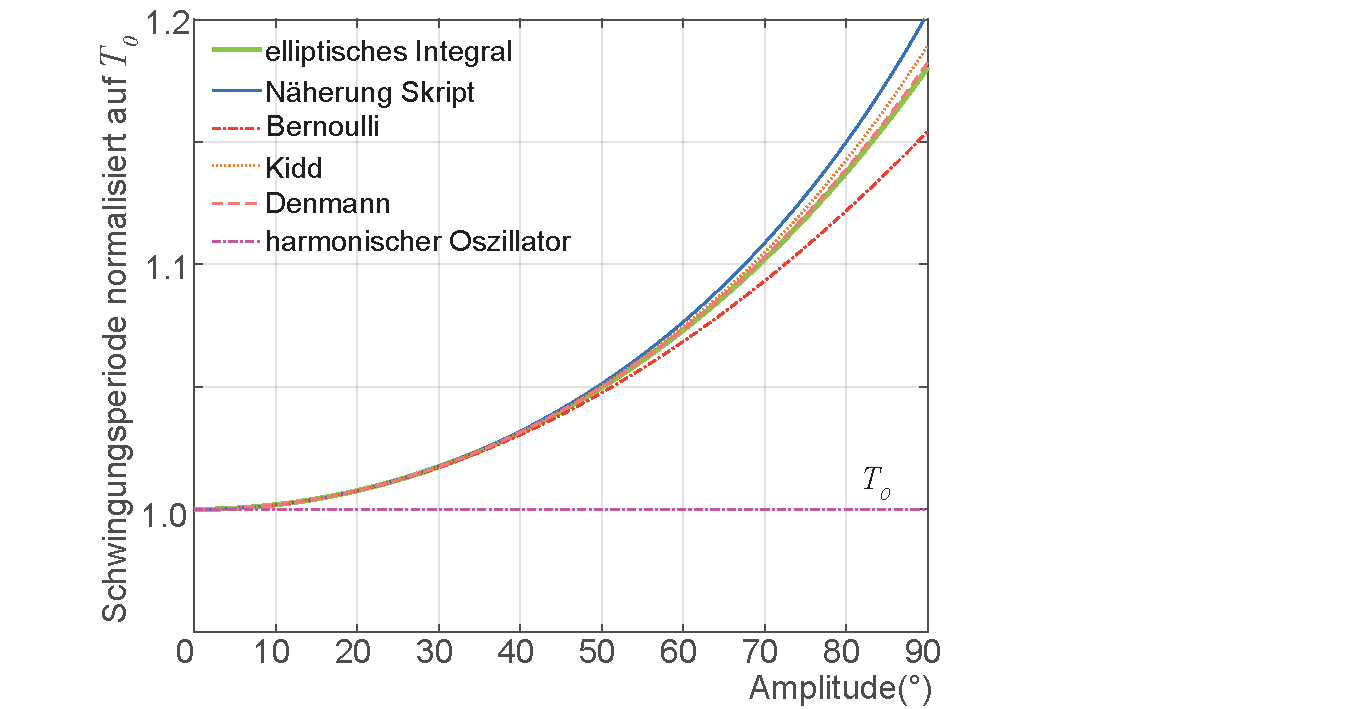
\includegraphics[width=\textwidth]{AnHarmonOsz01.pdf}
\caption[Schwingungsperiode des nichtlinearen Pendels als Funktion der Amplitude.]{Schwingungsperiode $T$ des nichtlinearen Pendels als Funktion der Amplitude $\theta_\text{A}$. L�sung nach \eqref{eq:bew_NLOsz12} sowie verschiedene N�herungsl�sungen aus der Literatur \cite{Hinrichsen2021} im Vergleich zur exakten und zur harmonischen L�sung. } \label{abb:bew_NLOsz01}
\end{figure}

\subparagraph{\textbf{Analytische Berechnung der Schwingungsperiode des nichtlinearen Pendels}}

Wir gehen hierbei �hnlich vor wie bei der Behandlung des Zweik�rperproblems (\kap{bew_ZKP_EEKP}).
Wir wissen, dass die Energie eine Erhaltungsgr��e der Bewegung ist, also gilt
\begin{align}
  E &= \text{const} = T+U = \frac{m}{2}l^2\dot{\theta}^2+\underbrace{m\,g\,l\,(1-\cos\theta)}_{\substack{U(\theta)}}  = m\,g\,l\,(1-\cos\theta_\text{A})  \nonumber \\
        &\rightarrow \frac{2\,(E-U(\theta))}{m\,l^2} = \lk \frac{\D\theta}{\D t}\rk^2~~\rightarrow~~\D t = \frac{\D \theta}{\sqrt{2\lek E - U(\theta) \rek/(m\,l^2)}}      \,. \label{eq:bew_NLOsz14}
\end{align}
Hierin ist $\theta_\text{A}$ die Amplitude des Pendels.
Wenn wir von $0$ bis $\theta_\text{A}$ integrieren, entspricht das einem Viertel  $T_\text{P}/4$  der Schwingungsperiode
	\begin{align}
			\frac{T_\text{P}}{4} = \int_{0}^{\frac{T_\text{P}}{4}} \D t = \bigintsss_{0}^{\theta_\text{A}} {\frac{\D \theta'}{\sqrt{\frac{2E-2U(\theta')}{m\,l^2}}}} = \sqrt{\frac{l}{2g}} \bigintsss_{0}^{\theta_\text{A}}\frac{\D \theta'}{\sqrt{\cos\theta'-\cos\theta_\text{A}}} \,. \label{eq:bew_NLOsz15}
	\end{align}
Mit $\cos x = 1-2\sin^2\frac{x}{2}$ erhalten wir
	\begin{align}
			\frac{T_\text{P}}{4} = \frac{1}{2}\sqrt{\frac{l}{g}} \bigintsss_{0}^{\theta_\text{A}}\frac{\D \theta'}{\sin\frac{\theta_\text{A}}{2}\sqrt{1-\bigg[\sin\frac{\theta'}{2} / \sin\frac{\theta_\text{A}}{2}\bigg]^2}}~. \label{eq:bew_NLOsz16}
	\end{align}
Unter Verwendung der Substitutionen 
    \begin{align*}
                z = \sin\frac{\theta'}{2} / k ~~~ \text{mit} ~~k = \sin\frac{\theta_\text{A}}{2}~~~\text{und} ~~~\D z = \frac{1}{2k}\cos\frac{\theta'}{2} \,\d \theta'  = \frac{1}{2k} \sqrt{1-k^2\,z^2} \,\D \theta' 
    \end{align*}
erhalten wir:
    \begin{align*}
                T_\text{P} = 4 \bigintsss_{0}^1 \frac{\D z}{\sqrt{(1-z^2)\,(1-k^2\,z^2)}} \,.
    \end{align*}
Mit der finalen Substitution $z = \sin\theta$ und der Periode des harmonischen Oszillators $2\pi\sqrt{l/g} = T_0 $
erhalten wir schlie�lich
    \begin{align}
                    T_\text{P} &= T_0 \frac{2}{\pi} \bigintsss_{0}^{\frac{\pi}{2}} \frac{\D\theta}{\sqrt{1-k^2\,\sin^2\theta}} = T_0 \frac{2}{\pi}\: \textbf{\textit{K}}(k)\: =\: T_0 \frac{2}{\pi}\: \textbf{\textit{K}}(\sin\frac{\theta_\text{A}}{2}) \,. \label{eq:bew_NLOsz17}
    \end{align}
    Hier ist $\textbf{\textit{K}}(k)$ das tabellierte \textit{vollst�ndige elliptische Integral erster Art}\index{Integral!elliptisches|textbf} \cite{Olver1992, Gradshteyn1980}, das nat�rlich auch numerisch mit \matlab{} berechnet werden kann \bzw dort auch als Funktion hinterlegt ist.

\subparagraph{\textbf{Methode der St�rungsrechnung zur Berechnung der Dynamik des nichtlinearen Pendels}}\index{St�rungsrechnung}

Gleichung \eqref{eq:bew_NLOsz17} ist gut geeignet, um eine Abh�ngigkeit der Schwingungsperiode von der Amplitude zu berechnen, siehe auch \figref{bew_NLOsz01}. 
Wir wollen nun noch die zeitliche Dynamik $\theta(t)$ des Systems betrachten.
Wir k�nnen diese nat�rlich aus 
\begin{align}
\ddot{\theta} + {\omega_0}^2 \sin\theta = 0  \label{eq:bew_NLOsz18}
\end{align}
numerisch berechnen oder L�sung \eqref{eq:bew_NLOsz03} benutzen mit $A_1 = \theta_\text{A}$ und $A_3$ gem�� \eqref{eq:bew_NLOsz07}.
Beide L�sungsvarianten sind im \mscr{} \mlbewref{AnHarmonOszillator02.m} ausgef�hrt und in \figref{bew_NLOsz02} auch im Vergleich zur harmonischen N�herung dargestellt.
Wie man erkennt, ist diese nur bis $\theta_\text{A} \approx 15\degree$ gut, wohingegen die N�herungsl�sungen auch noch bei $85 \degree$ brauchbare Ergebnisse liefern
(\figref{bew_NLOsz02}). Entwickeln wir die nichtlineare Schwingungsgleichung \eqref{eq:bew_NLOsz18} nach Potenzen von $\theta$ unter Benutzung der Abk�rzung $\Omega = \omega t$ und der Beziehung 
	\[\frac{\D }{\D t} \theta = \frac{\D \theta}{\D \Omega} \frac{\D \Omega}{\D t} = \theta' \, \omega\,,
\]
erhalten wir in der ersten nichtlinearen Ordnung die folgende zu Gleichung \eqref{eq:bew_NLOsz02} �quivalente DGL%
\footnote{Eine Differentialgleichung vom Typ $A\,y'' + B\,y + C\,y^3 = 0$ wird in der Literatur \cite{Kuypers2012} h�ufig als Duffing-DGL bezeichnet.}:
\begin{equation}
    \omega^2 \theta''(\Omega) + {\omega_0}^2 \theta(\Omega) - \kappa_3 \theta^3(\Omega) = 0~~~\text{mit}~~\kappa_3 = \frac{1}{6} {\omega_0}^2 \,.
    \label{eq:bew_StoerRe02}
\end{equation}
Wir wollen diese mit der Methode der St�rungsrechnung l�sen. Diese Methode wird in der Physik sehr h�ufig verwendet und wir werden ihr noch mehrmals begegnen.
F�r die L�sung der Differentialgleichungen \eqref{eq:bew_StoerRe02} betrachten wir die L�sung $\theta(\Omega)$ als zusammengesetzt aus der L�sung der linearen DGL $\theta_0(\Omega)$ und einem Zusatz, der aus der nichtlinearen St�rung $\sum\nolimits_i \kappa_i \theta^i$ folgt.
Ebenso betrachten wir die Schwingungsfrequenz $\omega$ als zusammengesetzt aus der L�sung f�r den linearen Fall $\omega_0$ und entsprechenden Zusatztermen.
Wir machen deshalb folgenden st�rungstheoretischen Ansatz, wobei wir f�r das nichtlineare Pendel nur die ungeraden Terme mitnehmen wollen\footnote{Die Rechnung f�r einen asymmetrischen Oszillator ist nat�rlich v�llig analog mit den zus�tzlichen geraden Termen.}:
\begin{align}
    \theta(\Omega) &= \theta_0(\Omega) + \kappa_3 \,\theta_1(\Omega) + {\kappa_3}^2 \,\theta_2(\Omega) + \ldots \nonumber \\
    \omega &= \omega_0 + \kappa_3 \,\omega_1 + {\kappa_3}^2 \,\omega_2 + \dots
    \label{eq:bew_StoerRe01}
\end{align}
Wir haben also angenommen, dass sich sowohl die L�sung selbst als auch die Eigenfrequenz des Pendels in Zusatztermen nach Potenzen der St�rungen darstellen lassen.
Wir setzen dies in \eqref{eq:bew_StoerRe02} ein und ordnen das Ergebnis nach Termen in Potenzen von $\kappa_3$, wobei jeder Term f�r sich verschwinden muss, da die Gleichung ja f�r alle Zeiten erf�llt sein muss:
%\begin{enumerate}[${\kappa_3}^1$:]
%    \setcounter{enumi}0
%  \item
%    ${\omega_0}^2 {\theta_0}'' + {\omega_0}^2 \theta_0 = 0 \label{eq:bew_StoerRe03a}$ \\
%  \item
%    ${\omega_0}^2 {\theta_1}'' + {\omega_0}^2 \theta_1 = {\theta_0}^3 - 2 \omega_0 \omega_1 {\theta_0}'' = 0  \label{eq:bew_StoerRe03b}$ \\
%  \item
%    ${\omega_0}^2 {\theta_2}'' + {\omega_0}^2 \theta_2 = 3 {\theta_0}^2 \theta_1 - ({\omega_1}^2 + 2\omega_0 \omega_2) {\theta_0}'' - 2 \omega_0 \omega_1 {\theta_1}''.$
%    \label{eq:bew_StoerRe03c}     
%\end{enumerate}
\begin{align}
    {\kappa_3}^0 :\quad &{\omega_0}^2 {\theta_0}'' + {\omega_0}^2 \theta_0 = 0 \label{eq:bew_StoerRe03a} \,,\\
    {\kappa_3}^1 :\quad &{\omega_0}^2 {\theta_1}'' + {\omega_0}^2 \theta_1 = {\theta_0}^3 - 2 \omega_0 \omega_1 {\theta_0}'' \,, \label{eq:bew_StoerRe03b} \\
    {\kappa_3}^2 :\quad &{\omega_0}^2 {\theta_2}'' + {\omega_0}^2 \theta_2 = 3 {\theta_0}^2 \theta_1 - ({\omega_1}^2 + 2\omega_0 \omega_2) {\theta_0}'' - 2 \omega_0 \omega_1 {\theta_1}''.
    \label{eq:bew_StoerRe03c}     
\end{align}
Man erkennt, dass die Gleichungen f�r die $\theta_i$ jeweils als Differentialgleichungen eines harmonischen Oszillators betrachtet werden k�nnen, die in den h�heren Ordnungen $\theta_i$ jeweils durch die niedrigeren Ordnungen angetrieben werden, also $\theta_1$ durch $\theta_0$, $\theta_2$ durch $\theta_1, \theta_0$ \usW
Die Anfangsbedingungen zur L�sung von \eqref{eq:bew_StoerRe02} sollen jeweils durch die nullte N�herung erf�llt werden, \dh
\begin{align}
    \theta_0 &= \theta_0(0) = \theta_A \qquad \text{(Anfangsamplitude)} \nonumber \\
    \dot{\theta_0} &= \dot{\theta_0}(0) = \dot{\theta_A} = 0 ~.
\end{align}
Damit sind alle $\theta_i(0)$ und $\dot{\theta_i}(0)$ f�r $i \geq 1$ gleich Null.
Die L�sung von \eqref{eq:bew_StoerRe03a} ergibt sich mit den Anfangsbedingungen zu
\begin{equation}
    \theta_0 = \theta_A \cos \Omega = \theta_A \cos \omega t \label{eq:bew_StoerRe04}~.
\end{equation} 
Setzen wir dies in \eqref{eq:bew_StoerRe03b} ein, erhalten wir f�r $\theta_1$ folgende DGL:
\begin{equation}
    {\omega_0}^2 {\theta_1}'' + {\omega_0}^2 \theta_1 = \lk \frac{3}{4} {\theta_A}^3 + 2 \omega_1 \omega_0 \theta_A \rk \cos \Omega + \frac{1}{4} {\theta_A}^3 \cos 3 \Omega
    \label{eq:bew_StoerRe05}~.
\end{equation}
Damit $\theta_1$ eine stabile Schwingungsl�sung ist, \dh nicht �ber alle Ma�en ansteigt,
muss der Term in der Klammer verschwinden%
\footnote{Der Beweis hierf�r sei als �bung empfohlen, auch eine numerische Rechnung f�r eine nichtverschwindende Klammer ist sehr instruktiv.},
woraus
\begin{equation*}
    \omega_1 = -\frac{3}{8} \frac{{\theta_A}^2}{\omega_0} \label{eq:bew_StoerRe06a}
\end{equation*}
folgt und somit f�r die Frequenz
\begin{align}
    \omega &= \omega_0 + \kappa_3 \omega_1 \nonumber = \omega_0 \lk 1 - \kappa_3 \frac{3}{8} \frac{{\theta_A}^2}{{\omega_0}^2} \rk = \omega_0 \lk 1 - \frac{ {\theta_A}^2}{16} \rk \,. \label{eq:bew_StoerRe06a}
\end{align}
erhalten.
Au�erdem ergibt sich daraus
\begin{equation}
    \theta_1 = \frac{1}{32} \frac{{\theta_A}^3}{{\omega_0}^2} (\cos\omega t - \cos 3 \omega t) \label{eq:bew_StoerRe06b}~.
\end{equation}
Wir sehen also, dass in erster N�herung nicht nur die Frequenz $\omega_0$ um $\kappa_3 \omega_1$ verschoben wurde, sondern dass auch in der Zeitdynamik ein Term $\kappa_3 \theta_1$ mit einer Oberschwingung bei $3 \omega$ hinzukommt.
Das Ergebnis ist somit sehr �hnlich dem, welches wir aus dem harmonischen Ansatz (vgl. \eqref{eq:bew_NLOsz12}) erhalten hatten.
Wir k�nnen jetzt noch die n�chste N�herungsordnung angehen.
Mit \eqref{eq:bew_StoerRe03c} und den trigonometrischen Identit�ten $\cos^3x = (3 \cos x + \cos 3x)/4$ sowie $\cos^2x = (\cos x + 2 \cos 3x + \cos 5x)/4$ findet man nach etwas Algebra
\begin{equation}
    {\omega_0}^2 \theta_2 '' + {\omega_0}^2 \theta_2
    = \lk \frac{21}{128} \frac{{\theta_A}^5}{{\omega_0}^2} + 2 \omega_0 \omega_2 \theta_A \rk \cos \Omega
    + \lk \frac{24}{128} \frac{{\theta_A}^5}{{\omega_0}^2} \rk \cos 3 \Omega
    + \lk - \frac{3}{128} \frac{{\theta_A}^5}{{\omega_0}^2} \rk \cos 5 \Omega
    \label{eq:bew_StoerRe07}~.
\end{equation}
Man erkennt, dass die Beitr�ge in den Klammern mit der Zunahme der Frequenz im $\cos$-Term immer kleiner werden,
wobei der erste Klammerterm wieder Null sein muss, damit es eine stabile L�sung gibt.
Wir erhalten damit als Bedingung 
\begin{equation}
     \omega_2 = - \frac{21}{256} \frac{{\theta_A}^4}{{\omega_0}^3} \label{eq:bew_StoerRe8a}
\end{equation}
und daraus 
\begin{equation}
    \theta_2 = \frac{1}{1024} \frac{{\theta_A}^5}{{\omega_0}^4} \lk 23 \cos \omega t - 24\cos 3 \omega t \rk~.
\end{equation}
Insgesamt ergibt sich also bis zur zweiten Ordnung der St�rungsrechnung
\begin{subequations}
\begin{align}
    \theta &= \theta_0 + \kappa_3 \theta_1 + {\kappa_3}^2 \theta_2 \nonumber \\
    &= \theta_A \lk 1 + \frac{{\theta_A}^2}{192} + \frac{23}{1024}\frac{{\theta_A}^4}{36}\rk \cos\omega t - \frac{{\theta_A}^3}{6} \lk \frac{1}{32} + \frac{{\theta_A}^2}{256} \rk \cos3\omega t + \frac{1}{1024} \frac{{\theta_A}^5}{36} \cos5\omega t \label{eq:bew_StoerRe09a} \\
		\text{und}  \nonumber \\
    \omega &= \omega_0 \lk 1 - \frac{1}{16} {\theta_A}^2 - \frac{7}{3072}{\theta_A}^4 \rk
    \label{eq:bew_StoerRe09b}~.
\end{align}
\end{subequations}
Es ist interessant, dass die Korrekturterme nur von der Anfangsamplitude und weiteren Konstanten abh�ngen, nicht aber von der Pendell�nge.
In \figref{bew_NLOsz02} haben wir auch L�sung \eqref{eq:bew_StoerRe09a} mit der numerischen L�sung der vollst�ndigen Pendelgleichung \eqref{eq:bew_NLOsz18} verglichen.

\begin{figure}
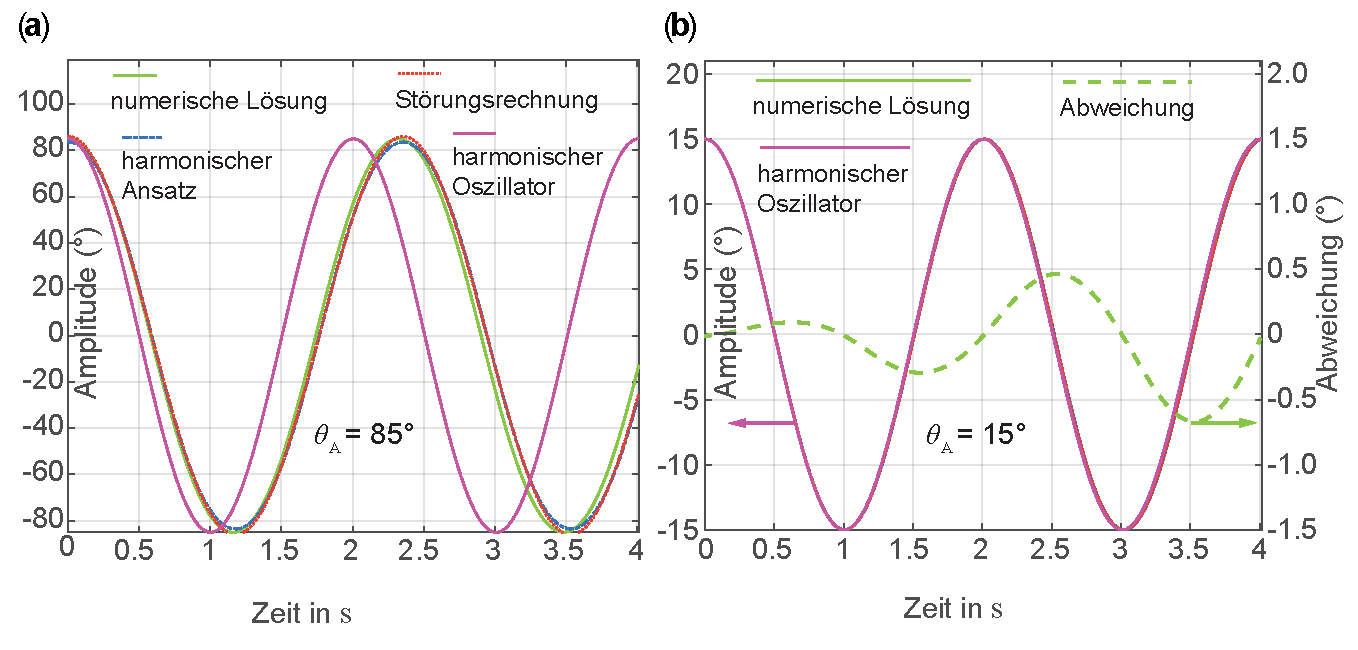
\includegraphics[width=\textwidth]{AnHarmonOsz02.pdf}
\caption[Schwingungsverhalten des nichtlinearen Pendels.]{Schwingungsverhalten $\theta(t)$ des nichtlinearen Pendels f�r verschiedene Amplituden $\theta_\text{A}$. Gezeigt sind verschiedene N�herungsl�sungen im Vergleich zur numerischen L�sung. \fa f�r Auslenkung $85\degree$ \fb f�r Auslenkung $85\degree$.} \label{abb:bew_NLOsz02}
\end{figure}


\subsubsection{Das Zykloidenpendel und die Brachistochrone} \index{Brachistochrone}\index{Pendel!Zykloidenpendel}\label{kap:bew_pendulum_zykl}

Wir hatten im vorhergehenden Kapitel gesehen, dass bei einem Fadenpendel die Schwingungsperiode von der Amplitude abh�ngt.
Da stellt sich die Frage, ob es eine M�glichkeit gibt, ein Pendel so zu konstruieren, dass die Schwingungsperiode unabh�ngig von der Auslenkung ist.\footnote{Dieses Problem war f�r die Uhrmacher des 17.~Jahrhunderts, \ua auch f�r Huygens, ein ganz reales.} Konkret sucht man also die Kurve, auf der sich ein Massepunkt mit konstanter Frequenz hin- und herbewegt, und zwar unabh�ngig von seiner maximalen Auslenkung.
Eine solche Kurve nennt man \emph{Tautochrone}.\footnote{Aus dem Griechischen f�r \textit{selbe Zeit}.}\index{Tautochrone}\\
Eng verwandt mit diesem Problem ist die Suche nach der Kurve im homogenen Schwerefeld, auf der ein sich reibungsfrei bewegender Massepunkt nur unter dem Einfluss der Gravitationskraft am schnellsten von einem Anfangspunkt $(x_\text{A},z_\text{A})$ zu einem gleich hoch oder tiefer gelegenen Endpunkt $(x_\text{E},z_\text{E})$ gelangt, wobei der Tiefpunkt der Bahn $(x_\text{T},z_\text{T})$ tiefer liegen kann als der Endpunkt.
Das Brachistochronenproblem wurde in einem Wettstreit zwischen den ziemlich verfeindeten Br�dern Jakob und Johann Bernoulli%
\footnote{Jakob Bernoulli (1655--1705) war ein Schweizer Mathematiker und Physiker, der wesentlich zur Entwicklung der Wahrscheinlichkeitstheorie sowie zur Variationsrechnung und zur Untersuchung von Potenzreihen beigetragen hat.\\
Johann Bernoulli (1667--1748) war Schweizer Mathematiker und Arzt und der j�ngere Bruder von Jakob Bernoulli.
Er arbeitete unter anderem auf dem Gebiet der Reihen und Differentialgleichungen und spielte eine wichtige Rolle bei der Entwicklung der Variationsrechnung.
So stellte er 1696 das Problem der Brachistochrone, das 1697 von ihm, seinem Bruder (sehr zu Johanns �rger), Newton (anonym) und Leibniz gel�st wurde.
Zur Geschichte und zu verschiedenen Ans�tzen zur L�sung des Brachistochronenproblems gibt es eine Reihe sch�ner Darstellungen \ua in \cite{Nahin2003, Shafer2007, Resch2018}.}%
\indexp{Bernoulli, Jakob}\indexp{Bernoulli, Johann} gel�st.
Damit wurden auch die Grundlagen der \emph{Variationsrechnung}\index{Variationsrechnung} geschaffen.
Wir wollen uns deshalb die Idee der Variationsrechnung zun�chst bei der Berechnung der Brachistochrone anschauen und das Ergebnis dann f�r die Beantwortung der Frage nach dem Pendel mit amplitudenunabh�ngiger Schwingungsperiode benutzen.

\subparagraph{\textbf{Brachistochrone}}

Die Kurve, auf der sich der Massepunkt bewegen soll, sei durch $z = f (x)$ gegeben (\figref{bew_Zykloid01}).
Die Lagrange-Funktion mit der unabh�ngigen Variablen $x$ ist dann gegeben durch
\begin{align}
	\mathcal{L} = \frac{m}{2} \lk\dot{x}^2 + \dot{z}^2 \rk + m\,g\,z = \frac{m}{2} \lk 1 + \lek f'(x)\rek^2 \rk \dot{x}^2 - m\,g\,f(x) \,. \label{eq:bew_Zykloid01}
\end{align}
Hierbei haben wir benutzt:
	\[\dot{z}= \frac{\D z}{\D t} = \frac{\D z}{\D x} \frac{\D x}{\D t} = z'(x)\,\dot{x} = f'(x)\,\dot{x} \,.
	\]
Ferner schreiben wir die Anfangs- und Randbedingungen wie folgt:
	\[ z(0) = z_\text{A} = 0\,,\,z(T) = z_\text{E}\,,\, x(T) = x_\text{E},\, \dot{z}(0) = \dot{z}_\text{A} =\dot{x}(0) = \dot{x}_\text{A} = 0\,. 
\]
Entgegen der �blichen Konvention lassen wir $z$ in die negative Richtung laufen, ersetzen also $z \rightarrow  -z$ (\figref{bew_Zykloid01}).
So geschrieben ist die Lagrange-Funktion in unserem Fall nur noch von der Funktion $f(x)$ bzw. $f'(x)$ abh�ngig, k�nnte im allgemeinen Fall aber auch noch explizit von $x$ abh�ngen.
Wir k�nnen Bewegungsgleichung \eqref{eq:bew_Zykloid01} sofort integrieren, da Energieerhaltung (siehe \eqref{eq:bew_Hamilton_Fkt}) gilt:
\begin{align}
	E = \dot{x} \frac{\partial \mathcal{L}}{\partial \dot{x}} -  \mathcal{L} = \frac{m}{2} \lk 1 + \lek f'(x)\rek^2 \rk \dot{x}^2 + m\,g\,f(x) = m\,g\,f(x_\text{A})\,. \label{eq:bew_Zykloid02}
\end{align}
Hierbei haben wir $E(t_\text{A}) = m\,g\,f(x_\text{A})$ angenommen.
Wir k�nnen \eqref{eq:bew_Zykloid02} durch Trennung der Variablen $x$ und $t$ in impliziter Form l�sen und erhalten
\begin{align}
	T &= \int_{t_\text{A}}^{t_\text{E}}\, \D t = \bigintsss_{x_\text{A}}^{x_\text{E}} \sqrt \frac{1+\lek f'[x]\rek^2}{2g\,\lk f(x_\text{A}) - f(x) \rk}\, \D x  = \bigintsss_{x_\text{A}}^{x_\text{E}} \mathcal{F}\lk f(x)\,,f'(x) \rk \D x \,. \label{eq:bew_Zykloid03}
\end{align}
Im \mscr{} \mlbewref{Brachistochrone.m} haben wir die Zeiten $T_i$ als Funktion verschiedener Kurven $f_i(x)$ berechnet und in \figref{bew_Zykloid02} dargestellt.
Man erkennt, dass im dargestellten Fall weder die direkte Verbindung noch der Kreisbogen (wie von Galilei angenommen) die k�rzeste "`Fallzeit"' ergeben.%
\footnote{Wir weisen darauf hin, dass das Integral in \eqref{eq:bew_Zykloid03} ein sogenanntes uneigentliches Integral ist, da $f(0) = 0$ ist und dar�ber hinaus die Tangente an $f$ bei $x=0$ senkrecht steht und $f'$ damit unendlich gro� wird. Der Fall $x_\text{A} = x_\text{E}=0$ muss daher im Grenz�bergang gesondert betrachtet werden.}
Wir suchen nun bei festen Endpunkten ($x_\text{A},x_\text{E})$ die Kurve oder Kurven $z(x) = f_\text{min}(x)$, f�r die die Zeit $T_{\min}$ minimal wird.
$\mathcal{F}\lk f(x)\,, f'(x) \rk$ in \eqref{eq:bew_Zykloid03} ist ein sogenanntes \emph{Funktional}\index{Funktional}, \dh eine Funktion einer Funktion.
Es handelt sich um ein sogenanntes \emph{Variationsproblem}\index{Variationsproblem}.
F�r dieses kann man zeigen \cite{Schmutzer2005, Greiner2003, Suesskind2014}, dass das Integral
\begin{align}
  I &= \bigintsss_{x_\text{A}}^{x_\text{E}} \mathcal{F}\lk f(x), f'(x) \rk \D x = \bigintsss_{x_\text{A}}^{x_\text{E}} \mathcal{F}\lk z(x), z'(x) \rk \D x \label{eq:bew_Zykloid05}
\end{align}
nur dann ein Minimum (Extremum) annimmt, wenn folgende Gleichung erf�llt ist:
\begin{align}
		\frac{\D}{\D x} \frac{\partial \mathcal{F}(z,z')}{\partial z'} - \frac{\partial \mathcal{F}(z,z')}{\partial z} = 0 . \label{eq:bew_Zykloid06}
\end{align}

\begin{figure}
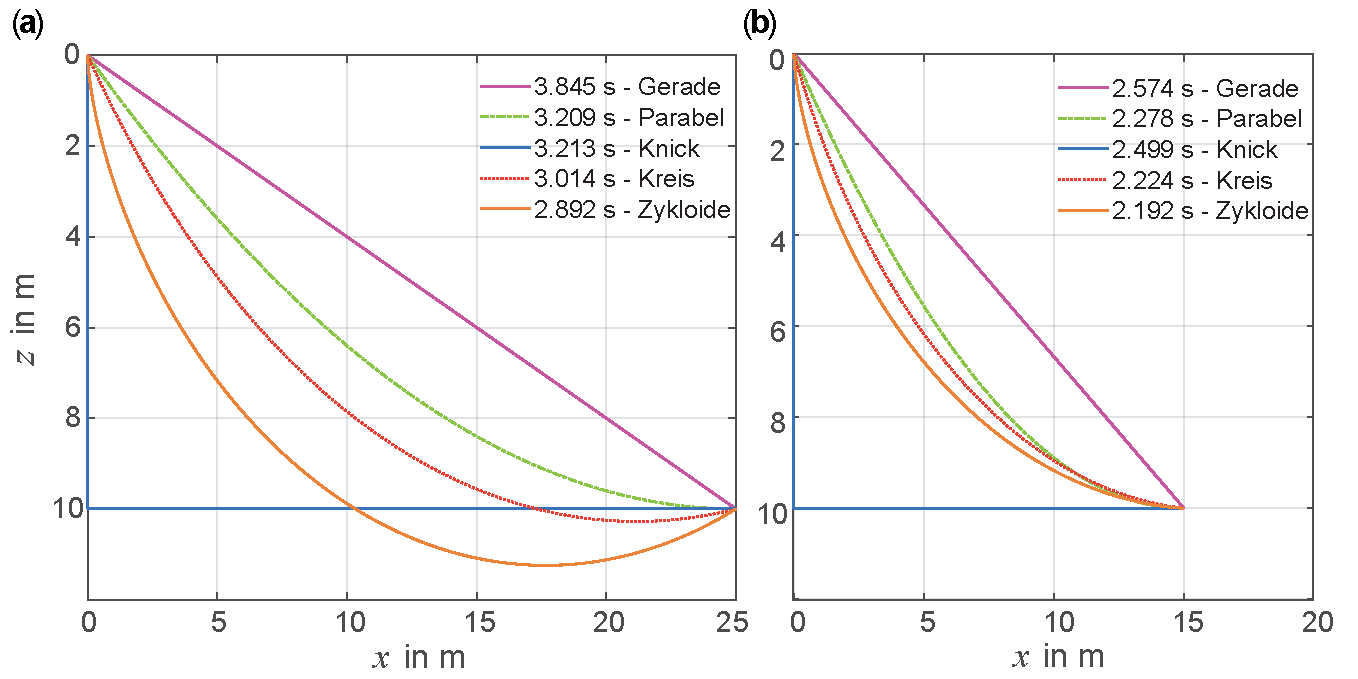
\includegraphics[width=\textwidth]{Zykloide01.pdf}
\caption[Verschiedene Fallkurven und deren Durchlaufzeiten.]{Fallkurven f�r eine Fallh�he von jeweils $\SI{10}{\metre}$ und deren Durchlaufzeiten f�r \fa eine Basisl�nge von $\SI{25}{\metre}$ und \fb eine Basisl�nge von $\SI{15}{\metre}$.} \label{abb:bew_Zykloid01}
\end{figure}

Diese Gleichung hei�t \emph{Euler-Lagrange-Gleichung}\index{Euler-Lagrange-Gleichung} und hat gro�e �hnlichkeit mit der Lagrange-Gleichung 2.\ Art
\eqref{eq:bew_LagrangeGl_II}, nur ist $\mathcal{F}$ hier ein \emph{Funktional} und $z=z(x)$ eine Funktion.%
\footnote{Die gleiche Struktur von \eqref{eq:bew_LagrangeGl_II} und \eqref{eq:bew_Zykloid06} ist nat�rlich nicht zuf�llig, sondern tief in der Struktur der Mechanik begr�ndet.
Wir empfehlen zur Vertiefung \cite{Schmutzer2005, Simonyi2004, Suesskind2014}.}
Damit k�nnen wir nun das Problem der Brachistochrone l�sen.
Wir schreiben f�r $\mathcal{F}\lk z(x)\,,z'(x)\rk$ in \eqref{eq:bew_Zykloid03} kurz als
\begin{align}
   \mathcal{F} =& \sqrt \frac{1+z'^2}{2g\, z}\,,  \label{eq:bew_Zykloid08}
\end{align}
womit man aus \eqref{eq:bew_Zykloid06} �ber folgende Schritte
\begin{align*}
    0 &=\frac{\D}{\D x}\,\frac{\d \mathcal{F}}{\d z'} - \frac{\d \mathcal{F}}{\d z}\, ~~~~ \Bigg|\,\cdot z'\pm z''\,\frac{\d \mathcal{F}}{\d z'} \\
    &= z'\,\frac{\D}{\D x}\,\frac{\d \mathcal{F}}{\d z'} - z'\,\frac{\d \mathcal{F}}{\d z} + z''\,\frac{\d \mathcal{F}}{\d z'} - z''\,\frac{\d \mathcal{F}}{\d z'} \\
    &= -\underbrace{\lk z'\,\frac{\d \mathcal{F}}{\d z}+z''\,\frac{\d \mathcal{F}}{\d z'}\rk}_{\frac{\D}{\D x} \mathcal{F}}+\underbrace{\lk z''\,\frac{\d \mathcal{F}}{\d z'}+z'\,\frac{\D}{\D x}\,\frac{\d \mathcal{F}}{\d z'}\rk}_{\frac{\D}{\D x}\lk z'\,\frac{\d \mathcal{F}}{\d z'}\rk}\\
    &= \frac{\D}{\D x}\,\lk z'\,\frac{\d \mathcal{F}}{\d z'}-\mathcal{F}\rk \\
    \intertext{als Zwischenergebnis}
    \Rightarrow \,& z'\,\frac{\d \mathcal{F}}{\d z'}-\mathcal{F} = \mathrm{const} = \hat{A}
\end{align*}
erh�lt. Mit \eqref{eq:bew_Zykloid08} ergibt sich daraus �ber 
\begin{align*}
    z'\,\frac{\d \mathcal{F}}{\d z'} &= \frac{1}{\sqrt{2g\,z}}\,\frac{{z'}^2}{\sqrt{1+{z'}^2}}\\
    \rightarrow \hat{A} &= z'\,\frac{\d \mathcal{F}}{\d z'}-\mathcal{F} =\frac{1}{\sqrt{2g\,z}}\lek \frac{{z'}^2}{\sqrt{1+{z'}^2}}-\sqrt{1+{z'}^2}\rek   =  \frac{1}{\sqrt{2g\,z}} \frac{{z'}^2+1-{z'}^2}{\sqrt{1+{z'}}}\, 
\end{align*}
schlie�lich die wichtige Beziehung 
\begin{align}
 1 + z'^2 = \frac{1}{\hat{A}^2\,2g} \frac{1}{z} = \frac{A}{z} \,. \label{eq:bew_Zykloid09}
\end{align}
Nach Trennung der Variablen erhalten wir
\begin{align}
		    \pm \D x &= \sqrt{\frac{z}{A-z}}\,\D z \,. \label{eq:bew_Zykloid09a}
\end{align}
Dies ist eine Differentialgleichung f�r $z(x)$, die wir mit dem Ansatz $z = A\sin^2\widetilde{\varphi}$ und $\D z = 2A\,\sin\widetilde{\varphi}\,\cos\widetilde{\varphi}\,\D \widetilde{\varphi}$ l�sen k�nnen:
\begin{align*}
    \D x &= 2A\,\sqrt{\frac{\killA{A}\,\sin^2\widetilde{\varphi}}{\killA{A}\,\lk 1-\sin^2\widetilde{\varphi}\rk}}\,\sin\widetilde{\varphi}\,\cos\widetilde{\varphi}\,\D \widetilde{\varphi}\\
    &= 2A\,\sin^2\widetilde{\varphi}\,\D\widetilde{\varphi} = A\lk 1-\cos 2\widetilde{\varphi}\rk\,\D \widetilde{\varphi} \,.
\end{align*}
Die Integration ergibt
\begin{align*}
    x &= A\lk \widetilde{\varphi}-\frac{1}{2}\,\sin 2\widetilde{\varphi}\rk + B = \frac{A}{2}\,\lk 2\widetilde{\varphi} -\sin 2\widetilde{\varphi}\rk +B \,,
\end{align*}
worin $B$ eine durch die Anfangsbedingungen festgelegte Integrationskonstante ist, die wegen $x_\text{A}=0$ als Null erkannt wird. Wir betrachten nur die positive $x$-Richtung, setzen 
$ 2 \widetilde{\varphi} \rightarrow\, \varphi$ und  $ A/2\, \rightarrow\, A$ und erhalten
\begin{align}
		x = A\lk\varphi - \sin{\varphi}\rk ~~\text{und}~~ z = A\lk 1 - \cos{\varphi}\rk \,. \label{eq:bew_Zykloid11}
\end{align}
Das ist aber gerade die parametrisierte Darstellung einer \emph{Zykloiden}.\index{Zykloide}
Eine solche Kurve wird von einem Punkt beschrieben, der sich auf dem Rand eines Rades befindet,
das entlang der x-Achse abrollt ohne zu gleiten.
Dabei sind $\varphi$ der Rollwinkel und $A$ der Durchmesser des Rades (\figref{bew_Zykloid02}).%
\footnote{Genau betrachtet ist die hier abgeleitete Brachistochrone die Spiegelung einer Zykloiden an der $x$-Achse.
Durch unsere Wahl der $z$-Koordinate in negativer Richtung kommen wir aber wieder auf die �bliche Zykloidendarstellung in Parameterform.
Als �bung sei empfohlen zu zeigen, dass \eqref{eq:bew_Zykloid11} tats�chlich eine Zykloide beschreibt und $A$ dem Durchmesser des abrollenden Rades entspricht.}
Die Brachistochrone ist also durch eine Zykloide gegeben, deren Parameter $A$ und $\varphi_\text{max} = \varphi_\text{E} $ sich aus den Anfangs- und Randbedingungen bestimmen lassen.
Insbesondere ergibt sich $\varphi_\text{E} $ aus
\begin{align}
	\frac{x(T)}{z(T)} = \frac{x_\text{E}}{z_\text{E}} = \frac{\varphi_\text{E}-\sin\varphi_\text{E}}{1 - \cos\varphi_\text{E}} \,. \label{eq:bew_Zykloid12}
\end{align}
Gleichung \eqref{eq:bew_Zykloid12} l�sst sich bis auf Spezialf�lle (Tab. \ref{tab:bew_Zykloid01}) nur numerisch l�sen.

\begin{table}[h!]
  \centering
   \begin{tabular}{ | C{2cm} | C{2cm}| C{2cm} | L{2cm} |} 
      \hline
            \rule{0pt}{2pt} & &  & \\
             $x_\text{E}$ & $x_\text{E}/z_\text{E}$& $\varphi_\text{E}$ & \\
            \rule{0pt}{2pt} & &  & \\
      \hline
            \rule{0pt}{2pt} & &  & \\
             \SI{0.0}{\metre} & 0.0  & nicht definiert & freier Fall \\
             \SI{10.0}{\metre} & 1.0  & & Neigung 45$\degree$\\
             \SI{15.7}{\metre} & $\pi/2$  & $\pi$ &  \\
             \SI{25.0}{\metre} & 2.5  &  &  \\
             \SI{31.4}{\metre} & $\pi$  &   & \\
              $\infty$ & $\infty$ & $2\pi$ &  \\
            \rule{0pt}{2pt} & &  & \\
      \hline
    \end{tabular}
    \medskip
    \caption[Parameter einer Zykloiden.]{Parameter einer Zykloiden. Siehe auch \figref{bew_Zykloid02}.}
    \label{tab:bew_Zykloid01}
\end{table}

\begin{figure}
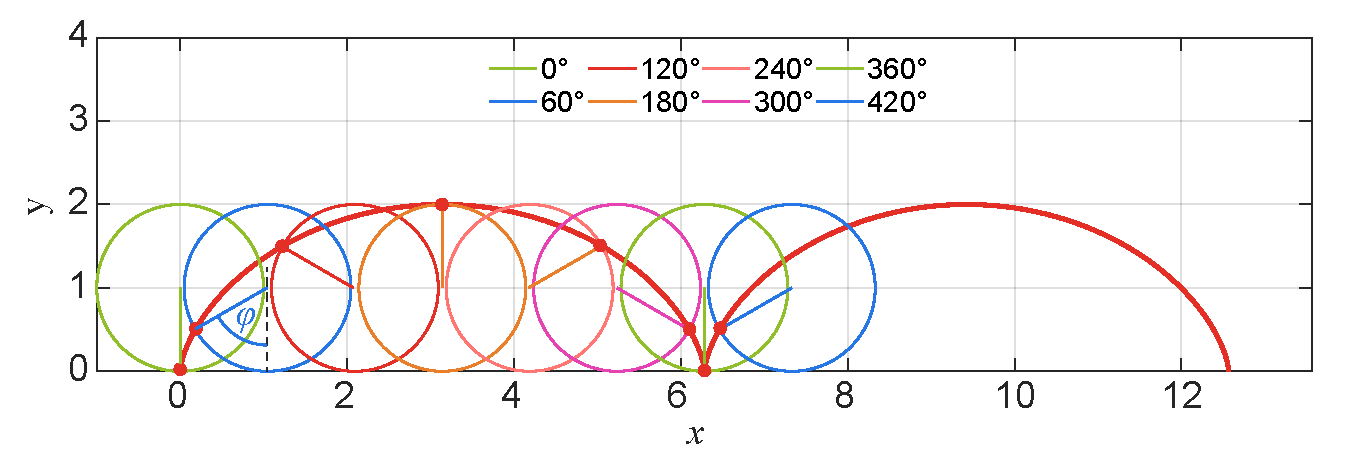
\includegraphics[width=\textwidth]{Zykloide02.pdf}%
\caption[Konstruktion einer Zykloiden.]{Konstruktion einer Zykloiden.} \label{abb:bew_Zykloid02}
\end{figure}

Wir k�nnen noch die gesamte Fallzeit entlang der Brachistochrone berechnen.
Wir starten mit Gleichung \eqref{eq:bew_Zykloid03} und formen diese leicht um:
\begin{align}
		T &= \bigintsss_{0}^{x_\text{E}} \sqrt{ \frac{ \lk\D x\rk^2 + \lk \D z\rk^2}{2g\,z} } \D x 
		   = \bigintsss_{0}^{\varphi_\text{E}} \sqrt {\frac{ A^2 \lk 1 - \cos\varphi \rk^2 + A^2 \lk \sin\varphi \rk^2}{2g\,A\lk 1 -\cos\varphi\rk} } \,\D \varphi \nonumber \\
		  &= \sqrt{\frac{A}{2g}}\bigintsss_{0}^{\varphi_\text{E}} \sqrt {\frac{ 1 - 2\cos\varphi  + \cos^2\varphi + \sin^2\varphi}{\lk 1 -\cos\varphi\rk} } \,\D \varphi \nonumber \\
                  &= \sqrt{\frac{A}{2g}}\bigintsss_{0}^{\varphi_\text{E}} \sqrt {\frac {2\,\lk 1 - \cos\varphi \rk}{\lk 1 -\cos\varphi \rk} } \,\D \varphi
		   = \sqrt{\frac{A}{g}}\bigintsss_{0}^{\varphi_\text{E}} \D \varphi = \sqrt{\frac{A}{g}}\,\varphi_\text{E} \,,\label{eq:bew_Zykloid13}
\end{align}
worin sich $A$ aus der \anf{Fallh�he} $z_\text{E}$ �ber $A = z_\text{E}/(1-\cos\varphi_\text{E})$ bestimmt und $0 < \varphi_\text{E} < 2\pi$ ist.\\
Eine sehr sch�ne Brachistochrone aus dem 18.~Jahrhundert ist heute im Museum Galileo in Florenz zu sehen (\figref{bew_Zykloid04}).
Dort kann man die Laufzeit einer Kugel im direkten Vergleich zur schiefen Ebene erfahren.
Es ist in diesem Zusammenhang auch eine interessante Frage, ob man bei Notfallrutschen am Flugzeug eine Brachistochrone nachbilden sollte.
Als �bung sei empfohlen, den m�glichen Zeitgewinn einer Brachistochrone-Notfallrutsche bei 500 Passagieren gegen�ber einer einfachen schiefen Ebene zu berechnen (\mscr{} \mlbewref{Brachistochrone.m}). 

\subparagraph{\textbf{Tautochrone, Zykloidenpendel}}

\begin{figure}
\begin{minipage}{\textwidth}
\leftfigure{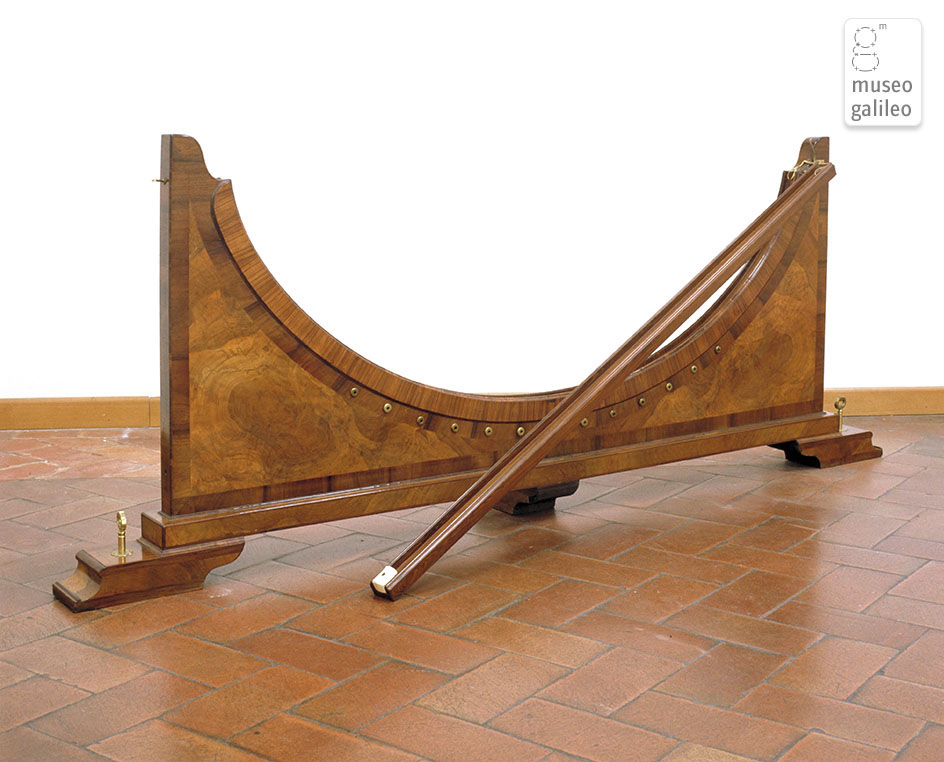
\includegraphics[width=0.5\textwidth]{Brachistochrone.jpg}}%
\hspace{\fill}
\rightfigure{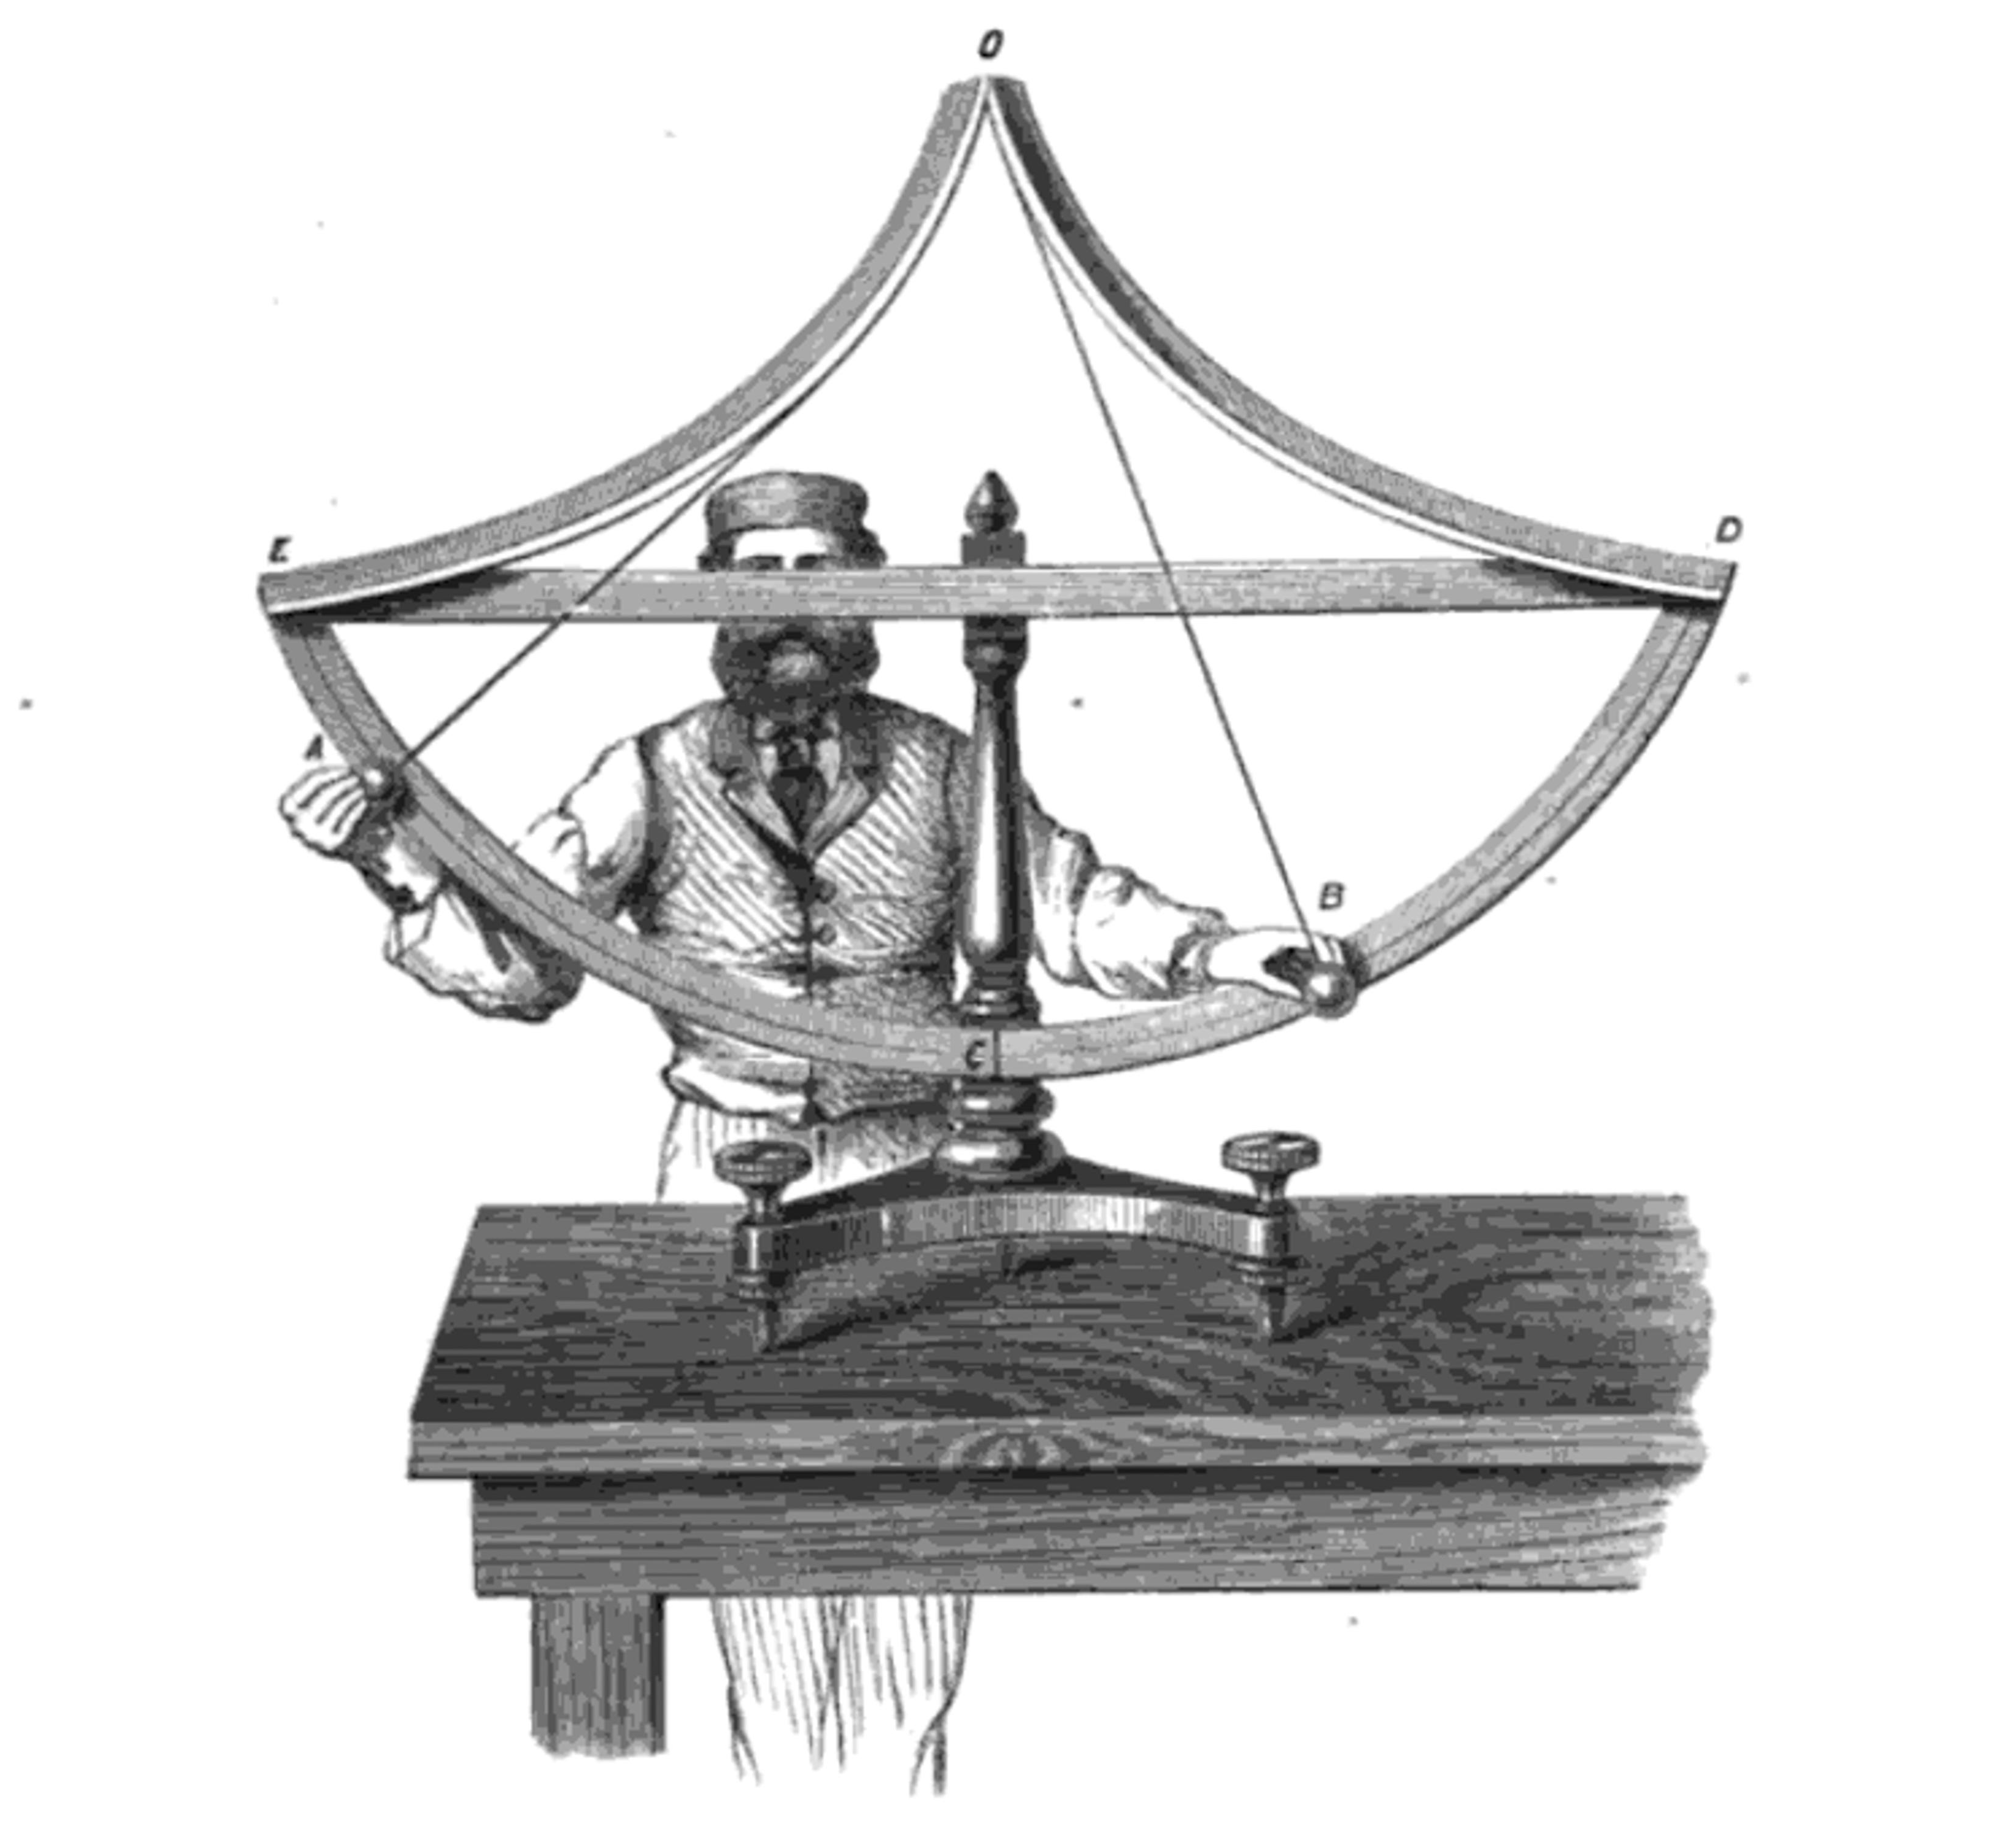
\includegraphics[width=0.5\textwidth]{Zykloidenpendel.jpg}}
\leftcaption[Brachistochrone aus dem Museo Galileo Florenz.]{Brachistochrone aus dem Museo Galileo Florenz. Gebaut von Francesco Spighi (Florenz, 2.\ H�lfte 18.~Jh.)\, \textcopyright Museo Galileo.} \label{abb:bew_Zykloid04}
\rightcaption[Konstruktion eines Zykloidenpendels.]{Konstruktion eines Zykloidenpendels.} \label{abb:bew_Zykloid05}
\end{minipage}
\end{figure}

Wir wissen also, dass die Brachistochrone eine Zykloide ist.
Nun untersuchen wir, wie die Bewegung auf derselben \bzw ihrer gespiegelten Kurve verl�uft.
Das \pot{} ist gegeben durch 
\begin{align}
	U = m\,g\,z = A\,\lk \cos\varphi - 1\rk \,.\label{eq:bew_Zykloid14}
\end{align}
Wir benutzen die Identit�t
\[ 1 - \cos\varphi = 2 \sin^2 \lk \frac{\varphi}{2} \rk \]
und erhalten mit $\varphi$ als generalisierter Koordinate die Lagrange-Funktion eines Teilchens, welches sich auf der Zykloidenbahn bewegt:
\begin{align}
    \mathcal{L} = \sin^2\frac{\varphi}{2}\,\lek \frac{m}{2} \lk 2A \rk^2 \dot{\varphi}^2 + m\,g\,\lk 2A \rk \rek \,.\label{eq:bew_Zykloid15}
\end{align}
Als Anfangs- \bzw Randbedingungen haben wir: $\varphi(0) = 0\,, \dot{\varphi}(0) = 0$ \bzw $0 < \varphi(x_\text{E}) < 2\pi$.
Durch die Substitution $q = \cos\frac{\varphi}{2}$ vereinfacht sich \eqref{eq:bew_Zykloid15} zu
\begin{align}
	\mathcal{L} = 8 m\, A^2\,\dot{q}^2 + 2m\,g\,A\, \lk 1 - q^2 \rk \,.\label{eq:bew_Zykloid16}
\end{align}
Die Lagrange-Gleichung \bzgl $q$ ergibt schlie�lich die Bewegungsgleichung eines Teilchens auf der Zykloide:
\begin{align}
	\ddot{q} = - \frac{g}{4A} q = {\omega_\text{zyk}}^2\,q \,.\label{eq:bew_Zykloid17}
\end{align}
Das ist aber die Bewegungsgleichung einer harmonischen Schwingung mit der \\
Kreisfrequenz $\omega_\text{zyk}$.
Im Gegensatz zum Pendel nach Gleichung \eqref{eq:bew_pendulum04} ist also die Bewegung auf der Zykloide exakt harmonisch, die Schwingungsfrequenz ist unabh�ngig von der Amplitude.
Damit ist die Zykloide eine Tautochrone.
Betrachtet man eine Zykloide, deren tiefster Punkt bei $(x_\text{T},\,z_\text{T})$ liegt, dann kommt ein Massepunkt an diesem Tiefpunkt immer zur gleichen Zeit an, ganz egal, von welcher H�he $z_\text{A}$ aus er startet.
Bereits Huygens erkannte dies und konstruierte eine Pendeluhr, die auf der Eigenschaft des Zykloidenpendels beruht.
Dies ist ein Pendel, bei dem der Faden zwischen zwei Zykloidenb�gen h�ngt und genau die L�nge des halben Zykloidenbogens hat (\figref{bew_Zykloid05}).
Dann beschreibt auch die Masse am Fadenende genau eine (gespiegelte) Zykloide.
Leider musste Huygens feststellen, dass die Gangungenauigkeit aufgrund der erh�hten Reibung an den Auflagefl�chen gr��er war als der Genauigkeitsgewinn durch die tautochrone Schwingung. \\


\subsubsection{Parametrische Oszillatoren -- Schaukel} \index{Oszillator!parametrischer}\label{kap:bew_pendulum_param}

Ein parametrischer Oszillator ist ein schwingendes System mit zeitabh�ngigen Parametern, durch die \zb Eigenfrequenz und D�mpfung ver�ndert werden k�nnen.
Dem Oszillator kann auf diese Weise Energie zugef�hrt werden, um die Amplitude der Schwingung zu vergr��ern.
Das am h�ufigsten zitierte Beispiel ist das Schwungholen bei einer Schaukel durch periodisches Heben und Senken des Schwerpunkts des schaukelnden K�rpers.
Ein solcher Oszillator mit rein parametrischer Anregung l�sst sich durch folgende homogene lineare Differentialgleichung beschreiben:
\begin{align}
		\ddot {x}+p_{1}(t){\dot {x}}+p_{2}(t) x=0 \,.	\label{eq:bew_schaukel01a}
\end{align}
Die zeitabh�ngigen Parameter $p_{1}$ und $p_{2}$ lassen sich zu einer zeitabh�ngigen Anregungsfunktion zusammenfassen, die man auch Pumpfunktion des Systems nennt.
Im Fall der Schaukel ist dies nat�rlich die eigene K�rperkraft, die ein Heben und Senken des K�rperschwerpunktes bewirkt.
Ein Merkmal einer rein parametrisch erzeugten Schwingung ist, dass sie ohne eine anf�ngliche Auslenkung aus der Ruhelage nicht entstehen kann, denn f�r die Anfangsbedingungen $(x,{\dot {x}})=(0,0)$ erh�lt man immer ${\ddot {x}}=0$.
Wir werden aber sehen, dass es schon bei infinitesimalen (unbeabsichtigten oder thermisch bedingten) Auslenkungen zu einer parametrischen Oszillation auch aus der Null-Lage kommen kann.
Die parametrische Anregung kann aber auch durch eine Zwangserregung erg�nzt werden, so dass die Differentialgleichung \eqref{eq:bew_schaukel01a} inhomogen wird.
Man spricht dann von einer kombinierten Zwangs- und Parametererregung:
\begin{align}
		{\ddot {x}}+p_{1}(t){\dot {x}}+p_{2}(t){x}=p_{3}(t) \,.	\label{eq:bew_schaukel01b}
\end{align}
Von besonderem praktischem Interesse \zb bei der Schaukel ist der Resonanzfall, bei dem die Parameter $p_{1}(t)$ und $p_{2}(t)$ mit doppelter Eigenfrequenz des Oszillators zeitlich variieren (\probref{bew_schaukelI}). 

\begin{figure}
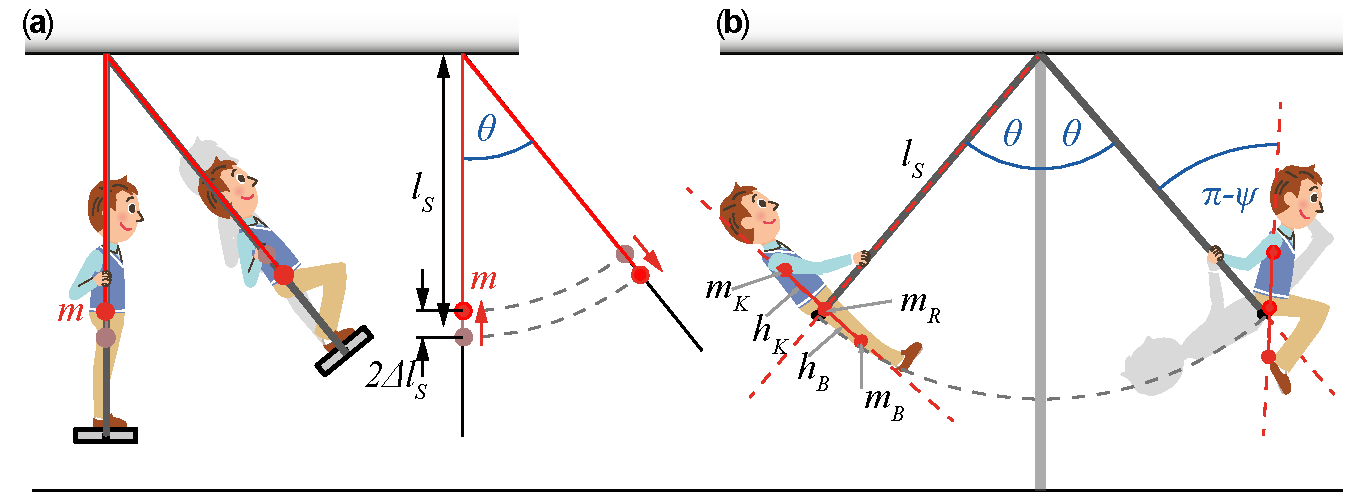
\includegraphics[width=\textwidth]{Schaukel01.pdf}
\caption[Modelle einer Schaukel.]{Modelle einer Schaukel. \fa Einfaches Massepunkt-Modell \fb Verbessertes Schaukelmodell mit sitzender Person als starren K�rper.}
\label{abb:bew_schaukel01}
\end{figure}

%\subparagraph{\textbf{Schaukelmodell a}}
Wir wollen zun�chst mit einem idealisierten Modell nach \figref{bew_schaukel01} a arbeiten und nur die Bewegung des Schwerpunktes entlang der Pendelaufh�ngung betrachten.
Bei Beginn des Schaukelns sei die Energie des Systems (\zb durch Ansto�en oder eine kleine Initialauslenkung) gegeben durch
        \begin{align}
            E_0 = m\,\frac{{v_0}^2}{2} = m\,g\,l_\text{S}\lk 1-\cos\theta_{\text{A}0}\rk\,. \label{eq:bew_schaukel01}
        \end{align}
Hierin ist $l_\text{S}$ die L�nge der Schaukel. Im Moment des Aufrichtens am Tiefpunkt verrichtet der Schaukelnde gegen die Schwer- und Zentrifugalkraft die Arbeit
        \begin{align}
            W_{\text{Unten}} = F\,\Delta l_\text{S} = \lk m\,g+\frac{m\,{v_0}^2}{l_\text{S}}\rk \,\Delta l_\text{S} \,, \label{eq:bew_schaukel02}
        \end{align}
wobei hierbei $F$ als ann�hernd konstant w�hrend der Bewegung angenommen wurde, was f�r ${\Delta l_\text{S}}/{l_\text{S}} \ll 1$ gut erf�llt ist. \\
Nach diesem \anf{Pumpen} im Durchgang durch den Tiefpunkt der Schaukel hat das System die Energie
        \begin{align}
            E_0' = E_0 + W_{\text{Unten}} = m\,g\,\Delta l_\text{S} +E_0\lk 1+ \frac{2\Delta l_\text{S}}{l_\text{S}}\rk \,.\label{eq:bew_schaukel03}
        \end{align}
Am Umkehrpunkt der Schaukel $\theta_\text{A}$ ist die Arbeit
    \begin{align}
        W_\text{Oben} = -m\,g\,\Delta l_\text{S}\,\cos\theta_{\text{A}} = -m\,g\,\Delta l_\text{S}+E_0'\,\frac{\Delta l_\text{S}}{l_\text{S}} \,, \label{eq:bew_schaukel04}
    \end{align}
und damit 
    \begin{align}
         E_0'' &= E_0' +  W_\text{Oben} = E_0 \lk 1+\frac{2\Delta l_\text{S}}{l_\text{S}}\rk + m\,g\,\Delta l_\text{S} - m\,g\,\Delta l_\text{S}\,\cos\theta_{\text{A}} \nonumber\\
        &= m\,g\,\Delta l_\text{S} \lk 1-\cos\theta_{\text{A}} \rk + E_0\lk 1+\frac{2\Delta l_\text{S} }{l_\text{S}}\rk = E_0'\,\frac{\Delta l_\text{S}}{l_\text{S}}+E_0\,\lk 1+\frac{2\Delta l_\text{S}}{l_\text{S}}\rk \\
        &=  m\, g\, \frac{\Delta l_\text{S}^2}{l_\text{S}} + E_0 \lk \frac{\Delta l_\text{S}}{l_\text{S}}+\frac{2\Delta l_\text{S}^2}{l_\text{S}^2}\rk+E_0\lk 1+\frac{2\Delta l_\text{S}}{l_\text{S}}\rk \approx E_0 \lk 1+\frac{3\Delta l_\text{S}}{l_\text{S}}\rk \,,
        \label{eq:bew_schaukel05}
    \end{align}
wobei wir wegen $\Delta l_\text{S} /l_\text{S} \ll 1$ quadratische Terme in $\Delta l_\text{S}$ vernachl�ssigen.
Nach einer vollen Periode haben wir zwei solcher Energie�nderungen $E_0''$, sodass nach $n$ Perioden 
        \begin{align}
            E_n =  E_0 \lk 1 + \frac{3\Delta l_\text{S}}{l_\text{S}} \rk^{2n} \,, \label{eq:bew_schaukel06}
        \end{align}
ist, wobei $n$ die Anzahl der Pendelperioden ist.
Die Beziehung f�r die Energie der Schaukel kann n�herungsweise geschrieben werden als 
        \begin{align}
            E_n =  E_0\, \mathrm{exp}\lk\frac{6n\,\Delta l_\text{S}}{l_\text{S}} \rk \,. \label{eq:bew_schaukel07}
        \end{align}
Es ist interessant zu bemerken, dass f�r dieses einfache System der relative Energiezuwachs $E_n/E_0$ nicht von der Masse abh�ngig ist (wohl aber von $\Delta l_\text{S}$).\\
Mit der Schwingungsperiode eines linearen Pendels mit
$T_\text{P}=2\pi\sqrt{l_\text{S}/g}$, $t=n\,T_\text{P}$ und $\Delta l_\text{S}/l_\text{S} = 2\Delta T_\text{P}/T_\text{P} = 2\Delta f/f = 2\,\Delta f\,T_\text{P}$
k�nnen wir \eqref{eq:bew_schaukel07} schreiben als
        \begin{align}
            E\lk t\rk = E_0\, \text{exp}\lk 12\:\Delta f\,t\rk \,. \label{eq:bew_schaukel08}
        \end{align}
Dies ist eine interessante Formel, die bis auf den Faktor 12 auch f�r sogenannte \emph{parametrische Oszillatoren und Verst�rker} \index{Verst�rker!parametrischer} G�ltigkeit hat.
Offensichtlich zeigt \eqref{eq:bew_schaukel08}, dass es f�r $E_0 = E\lk 0 \rk = 0$ keine parametische Verst�rkung geben kann.
Wenn man allerdings \zb durch die Luftbewegung eine Initialgeschwindigkeit von $v_0=\SI{1}{\cm\per\second}$ und die Parameter $m=\SI{50}{\kilogram}$, $l_\text{S}=\SI{3}{\metre}$ und $\Delta l_\text{S}=\SI{15}{\cm}$ annimmt, dann erh�lt man $E_0 = \SI{25e-4}{}\mathrm{Nm} $ und $f=\SI{0.29}{\per\second}$ und damit $E(t) = E_0\,\mathrm{exp}\lk{+12\,\Delta f\,t}\rk\approx E_0 \, \mathrm{exp}\lk{0.086\,t}\rk$.
Man erkennt, dass auch in diesem Fall die Energie schnell zunehmen kann und eine Auslenkung von $\theta_\text{A}=45\degree$ (wobei die harmonische N�herung, die wir hier benutzt haben, schon l�ngst versagt) nach ca.\ $t \approx \SI{4.6}{\second}$ erreicht wird. \\
Zur Berechnung der Zeitentwicklung k�nnte man dieses einfache Modell der Schaukel mit folgender DGL mathematisch beschreiben, wobei wir einen quadratischen Reibungsterm mitgenommen haben:
    \begin{align}
		\begin{split}
       &\ddot{\theta} + \eta\dot{\theta}^2+ \frac{l_\text{S}\lk t\rk}{g}\,\sin\theta = 0 ~~~ \text{mit}~~~ l_\text{S}\lk t\rk = l_\text{S}-\Delta l_\text{S} \,\cos\lk \omega_\text{A}\,t\rk  \,,\\
       &\ddot{\theta} + \eta\dot{\theta}^2+ \omega\lk t \rk\,\sin\theta = 0 ~~~ \text{mit}~~~ \omega\lk t\rk = \omega_0^2 - {\Delta\omega}^2 \,\cos\lk \omega_\text{A} \, t + \varphi_\text{A}\rk \,. 
		\end{split} \label{eq:bew_schaukel08a}
    \end{align}
    Wir l�sen diese numerisch im \mscr{} \mlbewref{Schaukel01.m} und zeigen das Ergebnis f�r verschiedene Parameter in \figref{bew_schaukel02}.

\begin{figure}
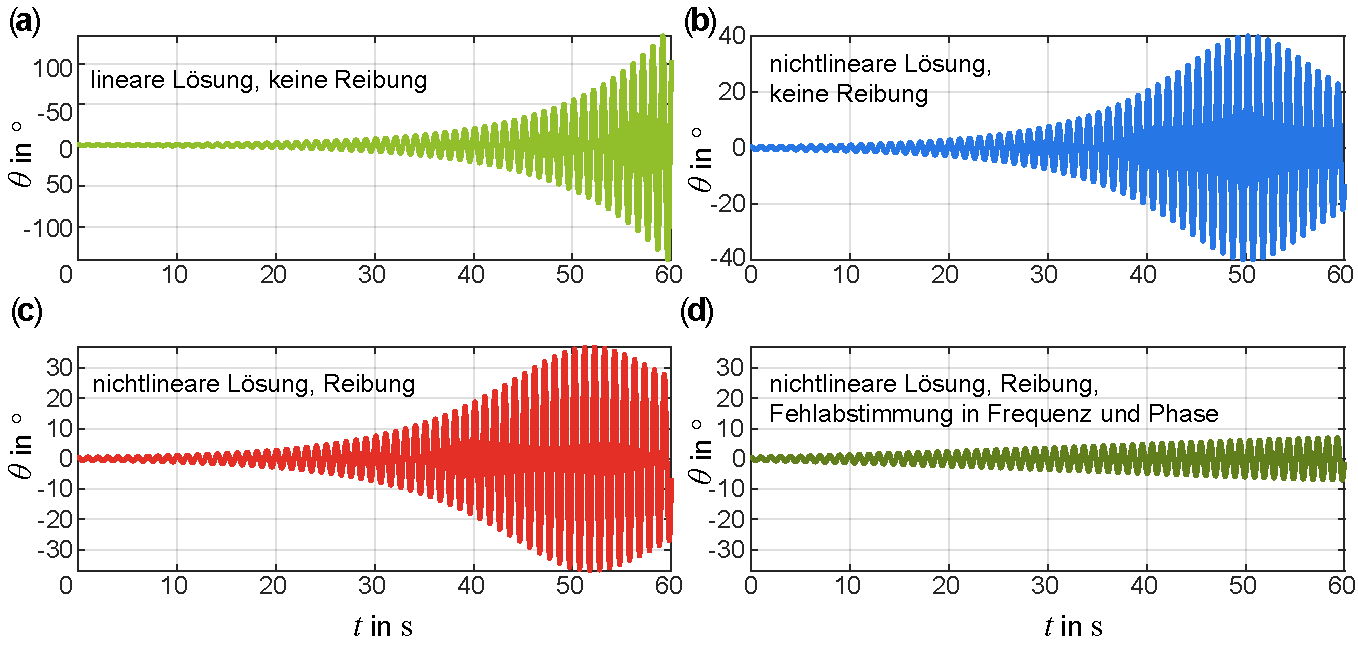
\includegraphics[width=\textwidth]{Schaukel04.pdf}
\caption[L�sung der Bewegungsgleichung eines parametrischen Oszillators.]{%
L�sung der Bewegungsgleichung f�r das Modell einer Schaukel als Beispiel eines parametrischen Oszillators.
Die Parameter aus \eqref{eq:bew_schaukel08a} sind: $\omega_0 = 2\pi\SI{}\second$, $\Delta\omega = 0.3\,\omega_0$, $\omega_\text{A} = 2\,\omega_0$ und $\varphi_\text{A} = 0$  (keine Fehlabstimmung), $\omega_\text{A} = 2.02\,\omega_0$ und $\varphi_\text{A} = \pi/4$  (Fehlabstimmung), $\eta = \SI{0.01}{\per\second\squared}$ (Reibung).
In der linearen N�herung \fa wurde die $\sin(\theta)$-Funktion in \eqref{eq:bew_schaukel08a} durch $\theta$ approximiert.
Man erkennt das exponentielle Aufschaukeln im Fall ohne Reibung, in der L�sung f�r den nichtlinearen Fall \fb -- \fd erzeugt die entstehende Fehlabstimmung der parametrischen Anregung automatisch eine Begrenzung und ein \anf{Abschaukeln}, man muss beim Schaukeln also die parametrische Frequenz der momentanen Eigenfrequenz anpassen, um Anregung zu erhalten.
\fc Ebenso entsteht eine zus�tzliche Begrenzung durch die Reibung. \fd Bei einer Fehlabstimmung in Frequenz und Phase erfolgt das Aufschaukeln deutlich langsamer.} \label{abb:bew_schaukel02}
\end{figure}

Wir wollten unsere Modellrechnung noch auf dem Spielplatz testen.
Bei der Beobachtung der schaukelnden Kinder stellen wir jedoch fest, dass anders als im Modell beschrieben, die meisten Kinder im Sitzen schaukeln und dabei eine Vor- und R�ckw�rtsbewegung des Oberk�rpers und der Beine ausf�hren, w�hrend der Schwerpunkt des K�rpers relativ zum Schaukelsitz mehr oder weniger in Ruhe bleibt.
Wir m�ssen also diese Bewegung in einem verbesserten Modell des schaukelnden K�rpers gem�� \figref{bew_schaukel01}b abbilden, was den Begriff des Tr�gheitsmoments\index{Tr�gheitsmoment} voraussetzt, den wir erst bei der Behandlung des starren K�rpers in \kap{bew_starrer_koerper} kennen lernen werden.
Wir werden dort in \kap{bew_pendulum_schaukel} dann auch ein verbessertes Modell der Schaukel angeben und durchrechnen.

\subsubsection{Das Foucault-Pendel} \index{Pendel!Foucault-}\index{Foucault-Pendel}\label{kap:bew_pendulum_foucault}

Bisher haben wir stillschweigend bei der Betrachtung der Pendelbewegung angenommen,
dass diese in einem Inertialsystem stattfindet. 
Wir wollen diese Annahme jetzt fallen lassen und fragen uns, wie die Pendelbewegung in einem mitrotierendem Koordinatensystem berechnet werden kann.
Wir betrachten dazu ein \emph{Foucault-Pendel}.
Diese Pendelanordnung mit gro�er Pendell�nge und -masse, die erstmalig 1851 von L�on Foucault%
\footnote{Jean Bernard L�on Foucault\indexp{Foucault, Jean Bernard L�on} (1819--1868) war ein franz�sischer Physiker und Astronom,
der bedeutende Beitr�ge auf dem Gebiet der Optik lieferte, aber auch im Design mechanischer Instrumente t�tig war.}
vorgestellt wurde, erm�glicht ohne zus�tzliche astronomische Beobachtungen den Nachweis der Erd\-rotation. 
Das Pendel wird dazu m�glichst reibungslos aufgeh�ngt,
wobei die Wirkung der Luftreibung im Verh�ltnis zur Gravitations- und Coriolis-Kraft
aufgrund der gro�en Masse vernachl�ssigt werden kann.
Das Prinzip ist recht einfach zu verstehen, denn die wesentliche Auswirkung der Rotation der Erde besteht darin, dass diese sich unter der im Inertialsystem feststehenden Schwingungsebene des Pendels wegdreht.
Am Nord- oder S�dpol ist dies am leichtesten einzusehen, weil der Aufh�ngepunkt des Pendels dort trotz der Erddrehung in Ruhe bleibt.
Daher w�rde die Erde sich an einem Tag\footnote{Genau gesprochen: einem Sternentag $=\SI{86164}{\s}$ (siehe Himmelsmechanik im Band II, Kapitel 3).} genau einmal voll unter dem Pendel hinwegdrehen.

\begin{figure}
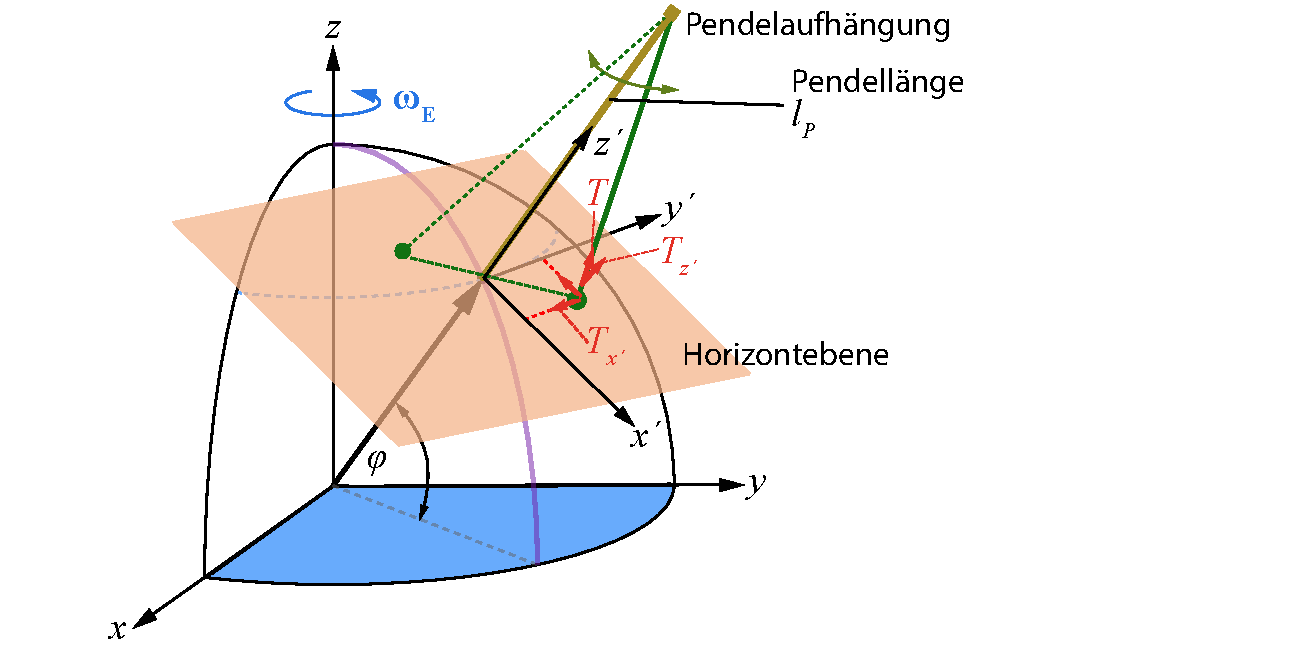
\includegraphics[width=\textwidth]{FoucaultPendel01.pdf}
\caption[Mitbewegtes Koordinatensystem f�r Foucault-Pendel.] {Mitbewegtes Koordinatensystem auf der Erdoberfl�che f�r die Betrachtung des Foucault-Pendels. Die Pendell�nge ist $l_\text{P}$ und die $T_{x'}', T_{y'}', T_{z'}'$ sind die Komponenten der Spannungskr�fte im Pendelarm im mitbewegten Koordinatensystem gemessen.}
\label{abb:bew_Foucault_01}
\end{figure}

In \kapitel{bew_Coriolis-Kraft} haben wir gesehen, wie die Scheinkr�fte auf bewegte K�rper f�r einen Beobachter im mitbewegten KOS wirken.
Bei einer Behandlung der Bewegung eines Foucault-Pendels im mitbewegten \KOS der Erde m�ssen diese Kr�fte nat�rlich im Rahmen der Newtonsche Mechanik mit ber�cksichtigt werden.
Wir starten dazu mit \eqref{eq:bew_BGL_Erdrotation} und erinnern uns,
dass die $x'$-Achse nach S�den und die $y'$-Achse nach Osten ausgerichtet ist (\figref{bew_Rot_Erde1}).
Unser Massepunkt soll jetzt an einem langen Faden der L�nge $l_\text{P}$ senkrecht auf der $x'$-$y'$-Ebene (also in $z'$-Richtung) aufgeh�ngt sein (\figref{bew_Foucault_01}).
Dann lautet die entsprechend aus \eqref{eq:bew_BGL_Erdrotation_Ko} abgeleitete Bewegungsgleichung f�r das Pendel
    \begin{align}
        \begin{pmatrix}
        \ddot{x}' \\
        \ddot{y}' \\
        \ddot{z}'
        \end{pmatrix}
        = -2\,\omega_\text{E}
        \begin{pmatrix}
        -\dot{y}'\sin\varphi \\
        \dot{x}'\sin\varphi + \dot{z}'\cos\varphi\\
        -\dot{y}'\cos\varphi + \frac{g}{2\omega_\text{E}}
        \end{pmatrix}
        + \frac{1}{m}
        \begin{pmatrix}
        T_{x'}' \\
        T_{y'}' \\
        T_{z'}'
        \end{pmatrix} \,,\label{eq:bew_BGL_Foucault}
    \end{align}
wobei wir vereinfachend die Zentrifugalkraft in eine effektive Erdanziehungskraft (Gravitation) eingeschlossen haben, also $F_\text{G} = m g$; der Winkel 
$\varphi$ ist wieder die geographische Breite. 
Die $T_\text{i'}'$ sind die Fadenspannungen in den drei Koordinaten, die die Masse an der Aufh�ngung halten (\figref{bew_Foucault_01}).

Wir wollen uns nun im wesentlichen die Projektion eines (relativ langen) Pendels auf die $x'$-$y'$-Ebene anschauen, sodass wir $\dot{z}'=0$ setzen k�nnen.
Aus \figref{bew_Foucault_01} sehen wir, dass f�r kleine Auslenkungen ${z'}/{l_\text{P}} \approx 1$ gilt und somit auch:
		\begin{align*}
				T_\text{z'}' &= -\,m\,g\,\frac{z'}{l_\text{P}} \approx m\,g \,, \\
				T_\text{x'}' &= -\,m\,g\,\frac{x'}{l_\text{P}}  \,, \\
				T_\text{y'}' &= -\,m\,g\,\frac{y'}{l_\text{P}} \,.
		\end{align*}
Zusammen mit der N�herung $\dot{z}'=0$ erhalten wir
		\begin{align}
				\begin{pmatrix}
				\ddot{x}' \\
				\ddot{y}'
				\end{pmatrix}
				= 
				\begin{pmatrix}
				+2\omega_\text{E}\,\dot{y}'\,\sin\varphi - \frac{g}{l_\text{P}}x'\\
				-2\omega_\text{E}\,\dot{x}'\,\sin\varphi - \frac{g}{l_\text{P}}y'
				\end{pmatrix} \,.
				\label{eq:bew_Foucault_02}
		\end{align}
Wir setzen ${\omega_0}^2= \frac{g}{l_\text{P}}$ als das Quadrat der Schwingungsfrequenz des Pendels der L�nge $l_\text{P}$ und k�nnen mit $Q = x'+i\,y' $ vorteilhaft die beiden Gleichungen aus \eqref{eq:bew_Foucault_02} zu einer komplexen Gleichung kombinieren:
		\begin{align}
				\ddot{Q} + 2 \mathrm{i} \,\omega_\text{F}\,\dot{Q}+{\omega_0}^2\,Q = 0  \qquad \text{mit} \qquad \omega_\text{F} = \omega_\text{E} \sin\!\varphi\,. \label{eq:bew_Foucault_03}
		\end{align}
Die Struktur dieser Gleichung entspricht der eines ged�mpften Oszillators \eqref{eq:bew_pendulum02}.
Deren L�sung war durch \eqref{eq:bew_pendulum04} gegeben, was hier nun bedeutet:
	\begin{align*}
		Q \lk t \rk &= x' +\im\,y'\\
		&= Q_0 e^{-\im\,\omega_\text{F}\,t}e^{\pm \im\,\hat{\omega}_0\,t} \qquad \text{mit} \qquad \hat{\omega}_0 = \sqrt{{\omega_0}^2+{\omega_\text{F}}^2}  \\
		&= Q_{01}\,e^{-\im\,\omega_\text{F}\,t}e^{\im\,\hat{\omega}_0\,t} + Q_{02}\,e^{-\im\,\omega_\text{F}\,t}e^{-\im\,\hat{\omega}_0\,t} \,.
	\end{align*}
Ganz allgemein k�nnen wir $Q_{01} = Q_{02} = \frac{Q_0}{2}$ setzen und erhalten
	\[Q \lk t \rk = Q_0\,e^{-\im\,\omega_\text{F}\,t}\cos\hat{\omega}_0 t = \lk x_0'+\im\,y_0'\rk \cos\hat{\omega}_0 t\,\lek\cos\omega_\text{F} t - \im\,\sin\omega_\text{F} t\rek \,,\]
sodass f�r $x(t)',\,y(t)'$ gilt:
    \begin{align}
        x'\lk t \rk &= + x_0'\cos\hat{\omega}_0 t\,\cos\omega_\text{F} t + y_0'\cos\hat{\omega}_0 t\,\sin\omega_\text{F} t \,,\notag\\
        y'\lk t \rk &= -x_0'\cos\hat{\omega}_0 t\,\sin\omega_\text{F} t + y_0'\cos\hat{\omega}_0 t\,\cos\omega_\text{F} t \,, \notag\\
    %\end{align*}
    \intertext{\bzw in Matrixschreibweise}
    %\begin{align}
        \begin{pmatrix}
            x'\lk t \rk \\
            y'\lk t \rk
        \end{pmatrix}
        &=
        \begin{pmatrix}
            +\cos\omega_\text{F}t & \, +\sin\omega_\text{F}t \\
            -\sin\omega_\text{F}t & \, +\cos\omega_\text{F}t
        \end{pmatrix}
        \begin{pmatrix}
            x_\text{P}'\lk t \rk \\
            y_\text{P}'\lk t \rk
        \end{pmatrix} \,,
        \label{eq:bew_Foucault_05}
    \end{align}
worin
		\begin{align*}
				x_\text{P}'\lk t \rk &= x_0'\cos\hat{\omega}_0 t + y_0' \cos\hat{\omega}_0 t = \lk x_0' + y_0' \rk \cos\hat{\omega}_0 t \quad \text{und} \\
				y_\text{P}'\lk t \rk &= \lk y_0' -x_0' \rk \cos\hat{\omega}_0 t
		\end{align*}
die Eigenl�sung des (harmonischen) Pendels ist. 
Die Matrix in \eqref{eq:bew_Foucault_05} ist offensichtlich eine Rotationsmatrix (siehe \kap{bew_rotating_systems}).
Damit beschreibt \eqref{eq:bew_Foucault_05} die zeitabh�ngige Drehung der Pendelebene, die durch die Vektoren $x_0'\lk t \rk \vecpeX + y_0'\lk t \rk \vecpeY ~\text{und} ~\vecpeZ$ aufgespannt wird.
Die Drehfrequenz $\omega_\text{F}$ h�ngt �ber $\omega_\text{F} = \omega_\text{E} \sin\varphi$ von der geographischen Breite ab,
sie ist am Pol maximal\footnote{Am Pol ist das Bild der Drehung der Pendelebene auch sehr anschaulich. F�r einen Beobachter im Inertialsystem steht die Ebene fest, die Beobachtungsebene dreht sich quasi unter der Aufh�ngung mit $\omega_\text{E}$ weg.} und verschwindet am �quator.
F�r das ber�hmte Foucault-Pendel im Deutschen Museum M�nchen ergibt sich
f�r das $\SI{60}{\metre}$ lange Seil und die geographische Breite von $\varphi = \SI{48.1}\degree$
eine Foucault-Rotationsperiode von 
\[T_\text{F} = \frac{2\pi}{\omega_\text{F}}\approx \SI{32}{\hour}\,\SI{8}{\minute}\]
bei einer Pendelperiode von $T_\text{P} = 2\pi\sqrt{\frac{l_\text{P}}{g}} \approx \SI{15.5}{\second}$.
Nach etwa $\SI{30}{\minute}$ hat sich die Pendel\-ebene also um etwa $\SI{5.6}\degree$ gedreht. \\
F�r ein deutlich schneller rotierendes KOS haben wir zur Veranschaulichung des Foucaultpendels in \figref{bew_Foucault_02} die Projektion des Pendels auf die $x$-$y$-Ebene dargestellt (siehe auch \mscr{} \mlbewref{FoucaultPendel.m}).

\begin{figure}
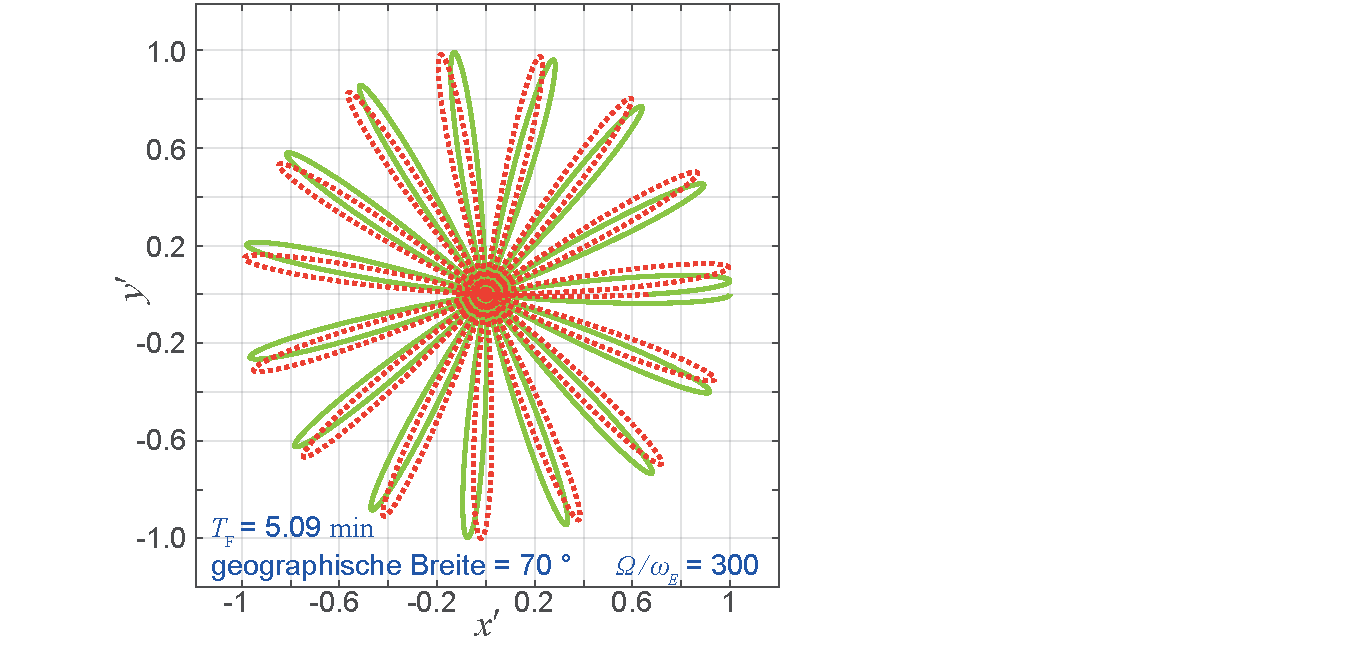
\includegraphics[width=\textwidth]{FoucaultPendel02.pdf}
\caption[Bahnkurve eines Foucault-Pendels bei "`schnellerer"' Erdrotation.] {Bahnkurve eines Foucault-Pendels bei einer angenommenen 300-fach schnelleren Erdrotation. Die Pendell�nge ist $\SI{100}{\metre}$. Dargestellt sind zwei Pr�zessionsperioden des Pendels. Man erkennt, dass die Rosettenbahn nicht ganz geschlossen ist, da $\omega_\text{F}$ kein ganzzahliges Vielfaches von $\omega_\text{E}$ ist.} 
\label{abb:bew_Foucault_02}
\end{figure}

\medskip

Zum Schluss wollen wir noch die Bewegungsgleichung des Foucault-Pendels �ber die Lagrange-Funktion herleiten.
Wir schreiben zun�chst die Lagrange-Funktion $\mathcal{L}$ f�r das Pendel im Inertialsystem auf:
\begin{align*}
		\mathcal{L} &= T-U =\frac{m}{2}\lek \dot{x}^2 + \dot{y}^2 + \dot{z}^2 \rek -U \lk x,y,z\rk\,.
\end{align*}
Aus der allgemeinen Transformation von KOS nach \eqref{eq:bew_Rot_System1} folgt insbesondere f�r ein rotierendes System mit $\vec{v} = \vec{v}' + \vec{\omega}' \times \vec{r}'$, dass
\begin{align*}
\vec{\omega}' = \omega_\text{E} 
	\begin{pmatrix}
		-\cos\varphi\\
		0 \\
		\sin\varphi
	\end{pmatrix}~. 
\end{align*}	
Damit ergibt sich die Bewegungsgleichung des Pendels zu
		\begin{align}
				\begin{pmatrix}
					\dot{x}\\
					\dot{y} \\
					\dot{z}
				\end{pmatrix}  
				&=
				\begin{pmatrix}
					\dot{x}'\\
					\dot{y}' \\
					\dot{z}'
				\end{pmatrix} 
				+s
				\begin{pmatrix}
					-\omega_\text{E}'\,y' \sin\varphi\\
					\omega_\text{E}'\,x' \sin\varphi + \omega_\text{E}'\,z' \cos\varphi \\
					-\omega_\text{E}'\,y' \cos\varphi
				\end{pmatrix} \,. 
				\label{eq:bew_Foucault_06}
		\end{align}
Bei Vernachl�ssigung von $\dot{z}', z'$ und $\omega'^2$ wird daraus jetzt in Koordinaten des rotierenden Systems
    \begin{align*}
      T & = \frac{m}{2} \lek \dot{x}'^2 + \dot{y}'^2 + 2 \omega_\text{E} \sin\varphi \lk x'\,\dot{y}'-\dot{x}'\,y'\rk\rek \,,\\
      \text{und} ~~~U &= m\,g\,\Delta z = m\,g\,\Delta z'= m\,g \lk l_\text{P}-l_\text{P}\cos\theta\rk = m\,g\,l_\text{P}\lk 1-\sqrt{1-\sin^2\theta} \rk \,,\\
      &\overset{\sin\theta \ll 1}{=} m\,g\,l_\text{P}\, \frac{1}{2}\sin^2\theta = \frac{m\,g\,l_\text{P}}{2}\lk\frac{x'^2+y'^2}{l_\text{P}{}^2}\rk \,, \\
      \text{mit} ~~ x'&= l_\text{P} \sin\theta\cos\phi \,,~~  y'= l_\text{P} \sin\theta\sin\phi \,.
    \end{align*}
Somit erhalten wir f�r die Lagrange-Funktion in Koordinaten des mitbewegten Systems
    \begin{align}
                    \mathcal{L} = \frac{m}{2} \lek \dot{x}'^2 + \dot{y}'^2 + 2\omega_\text{E}\sin\varphi \lk x'\,\dot{y}' - \dot{x}'\,y'\rk \rek - \frac{m\,g}{2\,l_\text{P}}\lk x'^2 + y'^2 \rk \,. \label{eq:bew_Foucault_07}
    \end{align}
�ber die Lagrange-Gleichungen ergeben sich sofort die Bewegungsgleichungen \eqref{eq:bew_Foucault_02}, ohne dass man weitere geometrische �berlegungen zu den Zwangskr�ften anstellen muss.
Man erkennt auch hier den Vorteil des Lagrange-Formalismus (Lagrange-Gleichungen zweiter Art).
In Zusatzaufgabe \ref{prob:bew_Zusatz_Foucault} werden die Bewegungsgleichungen des Foucault-Pendels exakt gel�st
und die kleinen Abweichungen von den in diesem Kapitel angestellten N�herungsl�sungen auf Basis der Newtonschen Mechanik diskutiert.


\subsubsection{Gekoppelte und komplexe Pendel} \index{Pendel!gekoppelte} \label{kap:bew_pendulum_coupled}

Wir wollen uns nun interessanten Beispielen f�r \emph{gekoppelte} schwingende Systeme aus Federn und Pendeln zuwenden.
Wir betrachten dabei zun�chst wieder geringe Auslenkungen, um ein Verfahren kennenzulernen,
das auch bei einer gro�en Zahl gekoppelter Elemente im schwingenden System gut anwendbar ist
und zugleich eine sch�ne Anwendung der linearen Algebra darstellt.
Anschlie�end betrachten wir zwei Beispiele: das Stangenpendel und das Doppelpendel.
Die Zwangsbedingungen des Doppelpendels hatten wir bereits in 
\probref{bew_Zwangsbedingungen} hergeleitet (siehe auch \figref{bew_Doppelpendel01}).\\

\subparagraph{Linearisierung gekoppelter Systeme bei geringen Auslenkungen}

Wir betrachten ein gekoppeltes schwingendes System mit $N$ Massepunkten und $Z_\text{B}$ Zwangsbedingungen.
Befindet sich dieses System nahe der Gleichgewichtslage, so lassen sich die Bewegungsgleichungen mit den verbleibenden $F = 3N-Z_\text{B}$ Freiheitsgraden entkoppeln, indem sogenannte Normalkoordinaten eingef�hrt werden.
Man erh�lt dann $F$ einfache entkoppelte Schwingungsgleichungen f�r jede dieser Koordinaten.
%Wir wollen das im Folgenden zeigen.
F�r ein solches System nahe der Gleichgewichtslage k�nnen wir dazu die Beziehungen
\eqref{eq:bew_Schwingung_b} und \eqref{eq:bew_Schwingung_a} f�r die kinetische Energie $T$ und die potentielle Energie $U$ verwenden.
Mit den generalisierten Koordinaten $q_i$ k�nnen wir durch
\begin{equation}
	\zeta_i = q_i - q_{i,0} \label{eq:bew_Kopplg01}
\end{equation} 
neue Koordinaten als Verschiebung von der Gleichgewichtslage (Auslenkung) einf�hren.
Dabei gilt $\dot{\zeta}_i = \dot{q}_i$.\footnote{Man macht sich das leicht klar, indem man in Gleichung 
\eqref{eq:bew_Schwingung_b} die Taylor-Entwicklung ausf�hrt.}
Wir schreiben
\begin{align}
	T &= \frac{1}{2}\sum_{i,j=1}^{F} \underbrace{\sum_{k=1}^{N} \lk m_k \frac{\partial x_k}{\partial q_i} \cdot \frac{\partial x_k}{\partial q_j} \rk \bigg|_{q_0}}_{T_{ij}} \dot{q}_i \dot{q}_j 
	= \frac{1}{2} \sum_{i,j=1}^{F} T_{ij} \dot{\zeta}_i \dot{\zeta}_j ~~ \text{und} \nonumber \\
	U &= \frac{1}{2} \sum_{i,j=1}^{F} \frac{\partial^2 U}{\partial q_i \partial q_j} (q_i - q_{0,i})(q_j - q_{0,j}) \nonumber \\
	&= \frac{1}{2} \sum_{i,j=1}^{F} \frac{\partial^2 U}{\underbrace{\partial \zeta_i \partial \zeta_j}_{U_{ij}}} \zeta_i \zeta_j = \frac{1}{2} \sum_{i,j=1}^{F} U_{ij} \zeta_i \zeta_j \label{eq:bew_Kopplg02} ~.
\end{align}
Die Lagrange-Funktion f�r das Gesamtsystem ist dann
\begin{align}
	\mathcal{L} &= T - U = \frac{1}{2} \sum_{i,j=1}^{F} T_{ij} \dot{\zeta_i} \dot{\zeta_j} - \frac{1}{2} \sum_{i,j=1}^F U_{ij} \zeta_i \zeta_j \,.\label{eq:bew_Kopplg03}
\end{align}
Daraus k�nnen wir die Lagrange-Gleichungen in einer einfachen Matrixdarstellung\footnote{Im Folgenden werden Grundkenntnisse der linearen Algebra wie Diagonalisierung, Eigenwertbestimmung, charakteristische Gleichung \usw vorausgesetzt. Wir empfehlen dem Leser zur Wiederholung die \onlineZ{}~ \bzw die Referenzen \cite{Arens2008, Riley2006, Fischer2018, Bartelmann2015}.} ableiten:
\begin{equation}
	\mathbb{T} \ddot{\vec{\zeta}} + \mathbb{U} \vec{\zeta} = 0 \qquad \text{mit} \qquad 
	\vec{\zeta} =
	\begin{pmatrix}
		 \zeta_1 \\ \zeta_2\\ \vdots \\ \zeta_F
	\end{pmatrix}\,,	\label{eq:bew_Kopplg04}
\end{equation}
worin die Matrizen $\mathbb{T}$ und $\mathbb{U}$ durch die $T_{ij}$ bzw. $U_{ij}$ bestimmt sind.\footnote{Es ist eine instruktive �bung, die Herleitung von \eqref{eq:bew_Kopplg04} aus \eqref{eq:bew_Kopplg03} zu zeigen.
Dazu m�ssen die Matrizen symmetrisch sein.
Dies ist durch die Definitionen \eqref{eq:bew_Kopplg01} und \eqref{eq:bew_Kopplg02} automatisch erf�llt.} Wir haben mit \eqref{eq:bew_Kopplg04} aber immer noch ein verkoppeltes System, da die Matrizen ja Nebendiagonalelemente haben, die genau die Kopplungen beschreiben.
Wir m�ssen also durch Einf�hrung neuer Koordinaten $\vec{\xi_i}$ (\dh eine Koordinatentransformation $\vec{\zeta}\rightarrow\vec{\xi}$) versuchen, das Problem zu diagonalisieren\footnote{Das Ziel besteht also darin, durch die Koordinatentransformation $\zeta \rightarrow \xi$ die Matrizen $\mathbb{T}$ und $\mathbb{U}$ gleichzeitig zu diagonalisieren.
Man kann zeigen, dass dies m�glich ist, da beide Matrizen symmetrisch sind \cite{Bartelmann2015, Riley2006}.} und die Lagrange-Funktion damit in die Form
\begin{equation}
	\mathcal{L} = \frac{1}{2} \sum_{i=1}^F {\dot{\xi_i}}^2 - \frac{1}{2} \sum_{i=1}^F \lambda_i {\xi_i}^2 \label{eq:bew_Kopplg05}
\end{equation}
zu bringen.
Daraus w�rden sofort die Lagrange-Gleichungen in der Form
\begin{equation}
	\ddot{\xi_i} + \lambda_i \xi_i = 0 \qquad i=1,2, \dots, F \label{eq:bew_Kopplg06}
\end{equation}
folgen.
Man erkennt aus \eqref{eq:bew_Kopplg06} und \eqref{eq:bew_Kopplg04}, dass die $\lambda_i$ mit den Eigenwerten der Matrix $\mathbb{U}$ zusammenh�ngen und daher folgende Eigenwertgleichung gilt, worin $\vec{n}_i$ die Eigenvektoren sind:
\begin{equation}
	\mathbb{U} \vec{n}_i - \lambda_i \mathbb{T} \vec{n}_i -  = 0 ~.\label{eq:bew_Kopplg07}
\end{equation}
Die Eigenwerte $\lambda_i$ entsprechen dem Quadrat einer Schwingungs-Kreisfrequenz und k�nnen damit als Eigenfrequenzen interpretiert werden.
Die entsprechenden Eigenvektoren $\vec{n}_i$ werden auch \emph{Eigenschwingungen} oder \emph{Eigenmoden}\index{Eigenmoden}\index{Eigenschwingungen} genannt.\\
Wie findet man nun diese Eigenfrequenzen und die dazugeh�rigen Eigenschwingungen $\vec{n}_i$?
Wir erinnern hier an die lineare Algebra\footnote{Das Eigenwertproblem hier weicht insofern von den typischerweise in der Algebra behandelten Eigenwertproblemen ab, als wir hier die Matrix $\mathbb{T}$ anstelle der Einheitsmatrix $\mathbb{I}$ verwenden.
Alle bekannten Regeln gelten aber f�r dieses modifizierte Eigenwertproblem genauso \cite{Riley2006, Fischer2018}.}, wonach zun�chst die zu \eqref{eq:bew_Kopplg07} geh�rende charakteristische Gleichung \index{Gleichung!charakteristische} \index{Eigenwert-Problem}
\begin{equation}
	\text{det}(\mathbb{U} - \vec\lambda \mathbb{T})  \overset{!}{=} 0 \label{eq:bew_Kopplg08}
\end{equation} 
zu l�sen ist. Aus den L�sungen $\lambda_i$ k�nnen dann die Eigenvektoren\index{Eigenvektor} $\vec{n}_i$ �ber \eqref{eq:bew_Kopplg07} bestimmt werden, woraus sich eine Transformationsmatrix $\mathbb{N} = n_{ij}$  bilden l�sst, mit der die Normalkoordinaten �ber $\vec{\xi} = \mathbb{N} \vec{\zeta}$ berechnet werden k�nnen.

\subparagraph{Gekoppeltes Stangenpendel}
\smallskip
Wir wollen nun die dargestellte Methodik an zwei Beispielen gekoppelter Systeme anwenden.
Dazu betrachten wir ein �ber eine Feder gekoppelte Stangenpendel und ein sogenanntes Doppelpendel.

\begin{figure}
\begin{minipage}{\textwidth}
\leftfigure{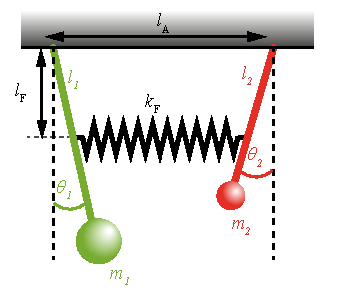
\includegraphics[width=0.5\textwidth]{GekoppeltePendel01.pdf}}%
\hspace{\fill}
\rightfigure{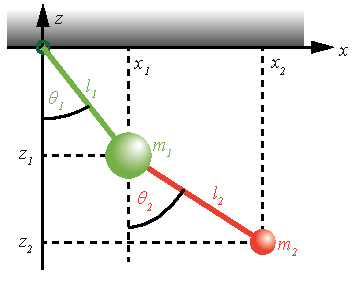
\includegraphics[width=0.5\textwidth]{DoppelPendel01.pdf}}
\leftcaption[Gekoppelte Stangenpendel.]{Gekoppelte Stangenpendel, die in der H�he $l_\text{F}$ durch eine Feder verbunden sind.}\label{abb:bew_Kopplg01}
\rightcaption{Geometrie des Doppelpendels.}\label{abb:bew_Doppelpendel01}
\end{minipage}
\end{figure}

Wir betrachten \figref{bew_Kopplg01} und bleiben zun�chst im Bereich geringer Auslenkungen.
Die Lagrange-Funktion lautet zun�chst ohne N�herungen
    \begin{align}
        \mathcal{L} &= \underbrace{\frac{m_1}{2} {l_1}^2 {\dot{\theta}_1{}}^2 + \frac{m_2}{2} {l_2}^2 {\dot{\theta}_2{}}^2}_T
        - g\,\underbrace{\lk  -m_1\, l_1\, \cos\theta_1 -m_2\,l_2\,\cos \theta_2 \rk}_{U_\text{Pendel}} \nonumber \\
        &\quad - \underbrace{\frac{k}{2} {l_\text{F}}^2 \lk (\sin\theta_1 - \sin\theta_2)^2 + (\cos\theta_1 - \cos\theta_2)^2\rk}_{U_\text{Feder}} 
        \label{eq:bew_Kopplg09} ~.
    \end{align}
Wir machen jetzt die N�herung
$l_i \sin\theta_i \approx l_i \theta_i$, sowie $\cos\theta_i \approx 1-\tfrac{{\theta_i}^2}{2} \approx 1$ und $l_\text{A} \geqq l_\text{F}$.
Zudem treffen wir die Annahmen
    \begin{align*}
        l_1 = l_2 = l_\text{F} \qquad \text{und} \qquad m_1 = m_2 = m~.
    \end{align*}
Wir erhalten damit f�r das vereinfachte und linearisierte Problem die Lagrange-Funktion in Matrix-Schreibweise
    \begin{align}
		\begin{split}
        \mathcal{L} =  
        \begin{pmatrix}
          \dot{\theta}_1 \\
          \dot{\theta}_2
        \end{pmatrix}^T
        \underbrace{
        m \,{l_\text{F}}^2 \begin{pmatrix}
        1 & 0 \\
        0 & 1
        \end{pmatrix}}_\mathbb{T}
        \begin{pmatrix}
          \dot{\theta}_1 \\
          \dot{\theta}_2
        \end{pmatrix}
        - 	
        \begin{pmatrix}
          \theta_1 \\
          \theta_2
        \end{pmatrix}^T
        \underbrace{ m \,g\,l_\text{F} 
        \begin{pmatrix}
          1 & 0 \\
          0 & 1
        \end{pmatrix}}_{\mathbb{U}_1}
        \begin{pmatrix}
          \theta_1 \\
          \theta_2
        \end{pmatrix} 
        \,- \begin{pmatrix}
          \theta_1 \\
          \theta_2
        \end{pmatrix}^T
        \underbrace{ k \,{l_\text{F}}^2 
        \begin{pmatrix}
          1 & -1 \\
          -1 & 1
        \end{pmatrix}}_{\mathbb{U}_2}
        \begin{pmatrix}
          \theta_1 \\
          \theta_2
        \end{pmatrix},
       \end{split} \label{eq:bew_Kopplg10}
    \end{align}
worin 
	$
        \begin{pmatrix}
                . \\
                .
        \end{pmatrix}
^T
$
	den transponierten Vektor darstellt.
Man erkennt an der Zerlegung von $\mathbb{U} = \mathbb{U}_1 + \mathbb{U}_2$, dass $\mathbb{U}_2$ nicht diagonal ist und die Kopplungsterme enth�lt.
Wir l�sen die charakteristische Gleichung \eqref{eq:bew_Kopplg08}:
    \begin{equation}
        {l_\text{F}}^2 \lk (m\,g + k \,l_\text{F} - m \,l_\text{F} \,\lambda)^2 - k^2\,{l_\text{F}}^2\rk = 0 \label{eq:bew_Kopplg11}~.
    \end{equation}
Diese hat als L�sungen die Eigenwerte
    \begin{align*}
        \lambda_1 = {\omega_1}^2 = \frac{g}{l_\text{F}} \qquad \text{und} \qquad \lambda_2 = {\omega_2}^2 =\frac{g}{l_\text{F}} + 2 \frac{k}{m}~.
     \end{align*} 
Die dazugeh�rigen Eigenvektoren bestimmen sich aus \eqref{eq:bew_Kopplg07}:
\[
\begin{pmatrix}
   m\,g\,l_\text{F} + k\,{l_\text{F}}^2 - \lambda_i\,m\,{l_\text{F}}^2  & -k\,{l_\text{F}}^2 \\
  - k\,{l_\text{F}}^2  & m\,g\,l_\text{F} + k \,{l_\text{F}}^2 - \lambda_i\,m \,{l_\text{F}}^2
\end{pmatrix}
\vec{n}_i = 0 ~~\text{und}~~\vec{n}_i= 	\begin{pmatrix}
  n_{1,i} \\
  n_{2,i}
\end{pmatrix} \,.
\]
Damit ergibt sich f�r den Eigenwert $\lambda_1$
\begin{align}
    \begin{pmatrix}
      +k\,{l_\text{F}}^2 &	-k\, {l_\text{F}}^2 \\
      - k\, {l_\text{F}}^2  & +k\, {l_\text{F}}^2
    \end{pmatrix}
    \begin{pmatrix}
      n_{1,1} \\
      n_{2,1}
    \end{pmatrix}
    &= 0 \qquad \implies \vec{n}_1 = \begin{pmatrix}
      1 \\1
    \end{pmatrix}
            \label{eq:bew_Kopplg12}\\
\intertext{und analog f�r $\lambda_2$}
        \begin{pmatrix}
          - k\,{l_\text{F}}^2 	& -k\,{l_\text{F}}^2 \\
          - k\,{l_\text{F}}^2 	& -k\,{l_\text{F}}^2
        \end{pmatrix}
        \begin{pmatrix}
          n_{1,2} \\ n_{2,2}
        \end{pmatrix}
        &= 0 \qquad \implies \vec{n}_2 = \begin{pmatrix} 1 \\ -1 \end{pmatrix}
        \label{eq:bew_Kopplg13}~.
\end{align}
Wir k�nnen die beiden Eigenschwingungen noch normalisieren, \dh wir fordern
\[
  {\vec{n}_i}^T ~ \mathbb{T} ~ \vec{n}_j = \delta_{ij}
\] 	 	
und erhalten schlie�lich die �berlagerung der beiden Normalschwingungen
\begin{equation}
    \begin{pmatrix}
      \theta_1(t) \\
      \theta_2(t)
    \end{pmatrix}
    = C_1 
    \begin{pmatrix} 1 \\ 1 \end{pmatrix} 
    \cos(\omega_1 t - \delta_1) 
    + C_2 
    \begin{pmatrix} 1 \\ -1 \end{pmatrix} 
    \cos(\omega_2 t - \delta_2) ~, \label{eq:bew_Kopplg14}
\end{equation}
wobei sich die Konstanten $C_1, C_2, \delta_1$ und $\delta_2$ aus den Anfangsbedingungen ergeben.
F�r eine passende Anfangsbedingung ist die L�sung von \eqref{eq:bew_Kopplg13} in \figref{bew_Kopplg02} gezeigt. Deutlich erkennt man das Auftreten einer Schwebung zwischen den Normalschwingungen.
Mit der Schwebung wandert die Energie quasi zwischen den beiden Pendeln hin und her.
Die numerische Rechnung (\mscr{} \mlbewref{GekoppeltePendel01.m}) zeigt f�r Winkel $<\SI{15}\degree$ gute �bereinstimmung mit \eqref{eq:bew_Kopplg14}.

\begin{figure}
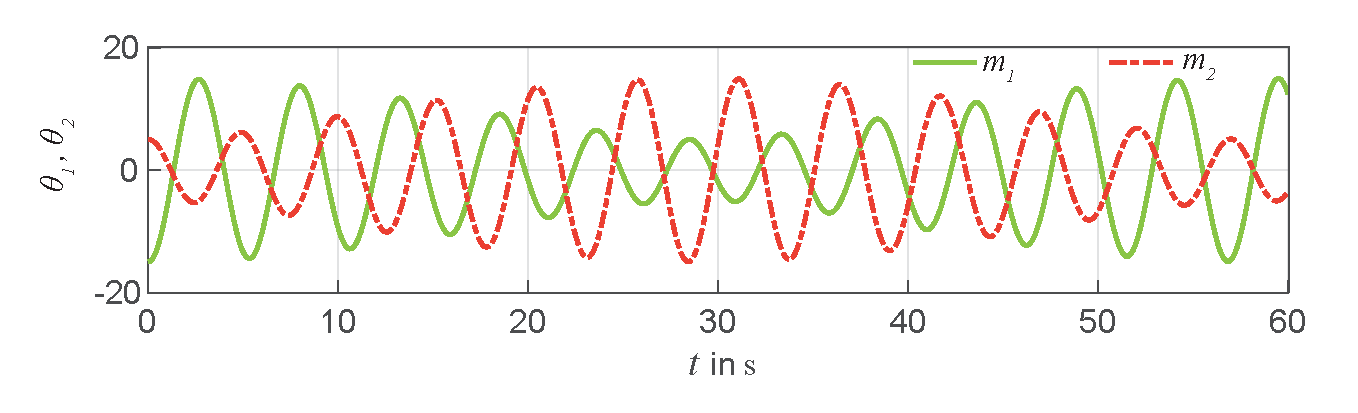
\includegraphics[width=\textwidth]{GekPendel01.pdf}%
\caption[Schwingungsverhalten zweier gekoppelter Stangenpendel.]{Schwingungsverhalten zweier gekoppelter Stangenpendel im Kleinwinkelfall und bei schwacher Kopplung. Deutlich ist das Schwebungsverhalten zu erkennen.}
\label{abb:bew_Kopplg02}
\end{figure}

Bisher haben wir uns in unserer Analyse auf kleine Winkel beschr�nkt und dar�ber hinaus gleiche Pendell�ngen und -massen angenommen.
Wir lassen nun f�r \probref{bew_Kopplung01} diese Begrenzungen fallen.
Die Rechnungen mit dem \mscr{} \mlbewref{GekoppeltePendel02.m} ergeben auch in diesem Fall f�r nicht zu starke Kopplungen $\keff$ das charakteristische Schwebungsverhalten (\figref{bew_Kopplg03}). Ebenso instruktiv ist es, in dem \mscr{}\, verschiedene Parameter wie \zb $\keff$ oder die relativen Pendell�ngen $l_1,\, l_2$ und -massen $m_1,\, m_2$ zu ver�ndern.

\begin{figure}
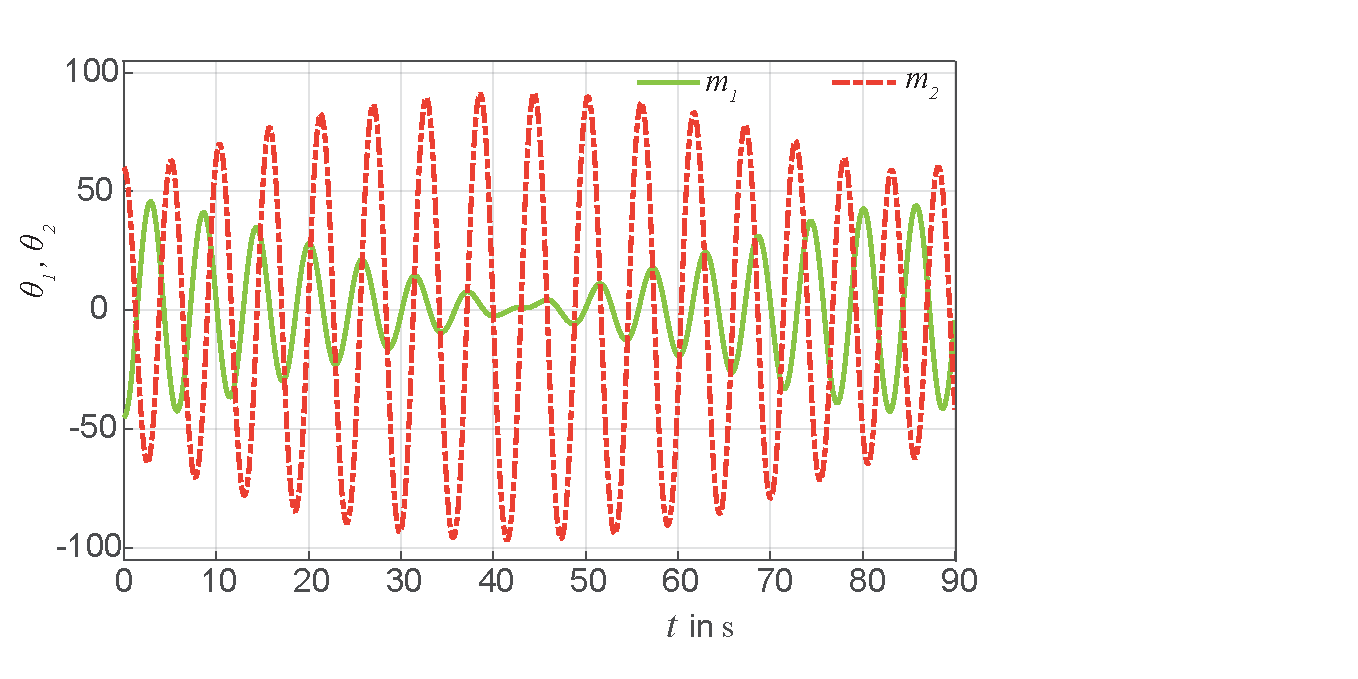
\includegraphics[width=\textwidth]{GekPendel02.pdf}%
\caption[Auslenkungen eines gekoppelten Pendels bei gro�en Auslenkungen.]{Auslenkungen eines gekoppelten Pendels bei gro�en Auslenkungen und schwacher Kopplung f�r folgende Parameter: $l_1 = \SI8\metre$, $l_2 = \SI6\metre$, $m_1 = \SI4{\kilo\gram}$, $m_2 = \SI3{\kilo\gram}$, $C_1 = 0.5$, $C_2 = 1$. Auch hier ist das Schwebungsverhalten deutlich zu erkennen.}
\label{abb:bew_Kopplg03}
\end{figure}

\subparagraph{Doppelpendel}

Diese Art des gekoppelten Pendels kann bei gr��eren Amplituden ein interessantes Verhalten zeigen, das auch als \anf{chaotisches Verhalten} bezeichnet wird.
Bevor wir dieses genauer anschauen, wollen wir die Bewegungsgleichungen des Doppelpendels aufstellen.
Unter Ber�cksichtigung der Zwangsbedingungen (\probref{bew_Zwangsbedingungen}) ergibt sich mit den generalisierten Koordinaten $\theta_1$ und $\theta_2$ die Lagrange-Funktion des Doppelpendels zu
\begin{align}
	\mathcal{L} &= \frac{m_1 + m_2}{2}\, {l_1}^2 \dot{\theta}_1{}^2 
	+ \frac{m_2}{2} {l_2}^2 \,{\dot{\theta}_2}{}^2 
	+ 2\,m_2 \,l_1\, l_2 \,\dot{\theta}_1 \,\dot{\theta}_2 \,\cos(\theta_1 - \theta_2) \nonumber \\
	&\quad + (m_1 + m_2) \,g \,l_1 \, \cos(\theta_1)
	+ m_2 \,g \,l_2 \,\cos(\theta_2) \,,\label{eq:bew_Doppelpendel01}
\end{align}
wobei wir konstante Terme im Potential \anf{weggeeicht} haben. 
Daraus lassen sich die Bewegungsgleichungen �ber
\[
\frac{\d \mathcal{L}}{\d t} \frac{\partial \mathcal{L}}{\partial \dot{\theta_i}} - \frac{\partial \mathcal{L}}{\partial \theta_i} = 0
\]
herleiten.
Man kann dabei gut von der symbolischen Toolbox von \matlab{} Gebrauch machen (siehe auch \mscr{} \mlbewref{Doppelpendel01.m}).
Wir erhalten
\begin{align}
	\ddot{\theta}_1 + \frac{g}{l_1}\,\sin\theta_1 + \frac{m_2}{m_1+m_2} \frac{l_2}{l_1} \
	\lek \ddot{\theta}_2\,\cos(\theta_2 - \theta_1) - {\dot{\theta}_2}{}^2 \,\sin(\theta_2 - \theta_1)  \rek 
	&= 0 \nonumber \quad \text{und}\\
	\ddot{\theta}_2 + \frac{g}{l_2}\sin\theta_2 + \frac{l_1}{l_2} \frac{m_1}{m_2} 
	\lek \ddot{\theta}_1 \,\cos(\theta_2 - \theta_1) - {\dot{\theta}_1}{}^2 \,\sin(\theta_2 - \theta_1)  \rek
	&= 0
	\label{eq:bew_Doppelpendel02}~.
\end{align}
Man erkennt an der Struktur der Lagrange-Gleichungen sehr sch�n, dass die beiden Pendelschwingungen durch die nichtlinearen Kopplungsterme (in den eckigen Klammern) gest�rt werden. 
F�r spezielle F�lle k�nnen wir aus \eqref{eq:bew_Doppelpendel02} wieder das sogenannte \anf{Kleinwinkelverhalten}, also die Bewegung bei geringen Auslenkungen, analytisch berechnen.
Wir nehmen dabei den einfachen Fall
\begin{align*}
	m_1 = m_2 = m 
	\quad \text{und} \quad 
	l_1=l_2 = l,
	\quad \text{sowie} \quad 
	\theta_1, \theta_2 \leqq 5\degree
\end{align*}
an, sodass gilt:
\begin{align*}
	\cos\theta_i &\approx 1~~~\text{und}~~~ \sin\theta_i \approx \theta_i,
	\quad {\dot{\theta_i}}^2 \theta_i \approx 0~.
\end{align*}
Die Lagrange-Gleichungen \eqref{eq:bew_LagrangeGl_II} vereinfachen sich damit erheblich zu
\begin{align}
	\ddot{\theta}_1 + \frac{g}{l} \theta_1 + \frac{1}{2} \ddot{\theta}_2 &= 0 \nonumber \\
	\ddot{\theta}_1 + \frac{g}{l} \theta_2 + \ddot{\theta}_2 &= 0~, 	\label{eq:bew_Doppelpendel03a}
\end{align}
\bzw in Matrixform
\begin{align}
    \begin{pmatrix}
 	 1  & 1/2 \\
	 1  & 1  
    \end{pmatrix}
    \begin{pmatrix}
 	\ddot{\theta}_1\\
 	\ddot{\theta}_2
    \end{pmatrix}
\, + \,
    \begin{pmatrix}
 	 g/l  & 0 \\
	 0    & g/l  
    \end{pmatrix}
    \begin{pmatrix}
 	\theta_1\\
 	\theta_2
    \end{pmatrix}
\, &= \, 0 \,.	\label{eq:bew_Doppelpendel03b}
\end{align}
Wir haben offensichtlich in dieser N�herung das DGL-System \textit{linearisieren} k�nnen und k�nnten damit nun einen der klassischen L�sungsans�tze (wie $\theta_i = \hat{\theta}_i \cos(\omega t)$) verfolgen.
Wir wollen hier aber bewusst die in diesem Kapitel eingef�hrte Methode �ber die charakteristische Gleichung \eqref{eq:bew_Kopplg08} verwenden. 
\Dh wir beginnen mit der Matrixform \eqref{eq:bew_Doppelpendel03b} und berechnen daraus direkt die Eigenfrequenzen $\lambda_{1,2} = (\omega_{1,2})^2$.
Die charakteristische Gleichung lautet dann\footnote{Als instruktive �bung wird empfohlen zu zeigen, dass die Ansatzmethode zu demselben Ergebnis f�hrt.}
\begin{equation}
    \begin{vmatrix}
	g/l - \lambda& -\lambda/2 \\
	-\lambda & g/l-\lambda
    \end{vmatrix} = 0 \label{eq:bew_Doppelpendel05}~. 
\end{equation}
Sie f�hrt uns zu den beiden Eigenwerten
\begin{equation}
	\lambda_{1,2} = {(\omega_{1,2})}^2 = \lk 2 \pm \sqrt{2}\rk \frac{g}{l} = \lk 2 \pm \sqrt{2}\rk {\omega_0}^2 \label{eq:bew_Doppelpendel06}~.
\end{equation}
Die Eigenmoden bestimmen wir �ber \eqref{eq:bew_Kopplg07}:\footnote{Alternativ setzt man die $\omega_i$ mit dem Ansatz in \eqref{eq:bew_Doppelpendel06} ein.
Wir erhalten dann f�r $\omega_1\!: \hat{\theta}_{2}^{(1)} = - \sqrt{2}\,\hat{\theta}_{1}^{(1)} $
und f�r $\omega_2\!: \hat{\theta}_{2}^{(2)} = + \sqrt{2}\,\hat{\theta}_{1}^{(2)}$.}
\[
\omega_1\,\text{:} ~n_{2,1} = - \sqrt{2}\,n_{1,1} ~~ \text{und} ~~ \omega_2 \,\text{:} ~n_{2,2} = + \sqrt{2}\,n_{1,2}\,.
\]
Das bedeutet, dass die beiden Pendel bei $\omega_1=\omega_\text{a}$ antisymmetrisch (also entgegengesetzt) schwingen und bei $\omega_2=\omega_\text{s}$ symmetrisch (also gleichgerichtet).
Die antisymmetrische Schwingungsfrequenz $\omega_\text{a}$ ist nach \eqref{eq:bew_Doppelpendel06} $1 + \sqrt{2} \approx 2.4$-fach so hoch wie die der symmetrischen Schwingung.
Das l�sst sich leicht verstehen, da die r�cktreibenden Kr�fte im antisymmetrischen Fall gr��er sind.
Im Rahmen der Kleinwinkeln�herung ist die allgemeine L�sung also durch eine �berlagerung der beiden Normalschwingungen gegeben:
\begin{align*}
    \begin{pmatrix}
 	\theta_1\\
 	\theta_2
    \end{pmatrix}
\, = \,
    \begin{pmatrix}
 	n_{1,1} & n_{1,2}\\
 	n_{2,1} & n_{2,2}
    \end{pmatrix} 
    \begin{pmatrix}
 	C_1\, \cos(\omega_\text{a} t + \delta_\text{a})\\
 	C_2\, \cos(\omega_\text{s} t + \delta_\text{s}) 
    \end{pmatrix}
\end{align*}
\bzw in komplexer Schreibweise
\begin{align}
	\theta_1(t) &= \lk A \text{e}^{\mathrm{i} \omega_\text{a} t} + B \text{e}^{-\mathrm{i}\omega_\text{a} t}\rk + \lk C \text{e}^{\mathrm{i}\omega_\text{s} t} + D \text{e}^{-\mathrm{i}\omega_\text{s} t} \rk \;,\nonumber \\
	\theta_2(t) &= -\sqrt{2} \lk A \text{e}^{\mathrm{i} \omega_\text{a} t} + B \text{e}^{-\mathrm{i}\omega_\text{a} t}\rk + \sqrt{2} \lk C \text{e}^{\mathrm{i}\omega_\text{s} t} + D \text{e}^{-\mathrm{i}\omega_\text{s} t} \rk \label{eq:bew_Doppelpendel07}~. 
\end{align}
W�hlen wir die Anfangsbedingungen \zb zu
\begin{align*}
	\theta_1(0) &= \theta_{10} = +(A+B) + (C+D) \,,\\
	\theta_2(0) &=\theta_{20} = -\sqrt{2} (A+B) + \sqrt{2} (C+D) \,,\\
	\dot{\theta}_1(0) &= \dot{\theta}_{10} = + \im\, \omega_\text{a} (A-B) + \im\, \omega_\text{s} (C-D) \,,\\
	\dot{\theta}_2(0) &= \dot{\theta}_{20} = - \im \sqrt{2}\, \omega_\text{a} (A-B) + \im \sqrt{2}\, \omega_\text{s} (C-D)\,, \\
\end{align*}
so ergibt sich
\begin{equation}
    \begin{pmatrix}
	+1 & +1 & +1 & +1 \\ 
	-1 & -1 & +1 & +1 \\
	+\mathrm{i} \omega_\text{a} & -\mathrm{i}\omega_\text{a} & +\mathrm{i}\omega_\text{s} & -\mathrm{i}\omega_\text{s} \\
	-\mathrm{i} \omega_\text{a} & +\mathrm{i}\omega_\text{a} & +\mathrm{i}\omega_\text{s} & -\mathrm{i}\omega_\text{s}
    \end{pmatrix}
    \begin{pmatrix} A \\ B\\ C\\ D\end{pmatrix}
    = 
    \begin{pmatrix}
	\theta_{10} \\ \theta_{20} /\sqrt{2} \\ \dot{\theta}_{10} \\ \dot{\theta}_{20} /\sqrt{2}
    \end{pmatrix}~.
\end{equation}
Wir l�sen dieses lineare Gleichungssystem in \matlab{} und erhalten die Werte der Koeffizienten $A$, $B$, $C$ und $D$. 
Damit k�nnen wir schlussendlich die Kleinwinkell�sung nach \eqref{eq:bew_Doppelpendel07} bestimmen. Diese vergleichen wir f�r $\theta_1, \theta_2 \leqq 5\degree$
mit der numerischen L�sung aus dem  \mscr{} \mlbewref{Doppelpendel02.m} und finden eine gute �bereinstimmung.\\

\begin{figure}
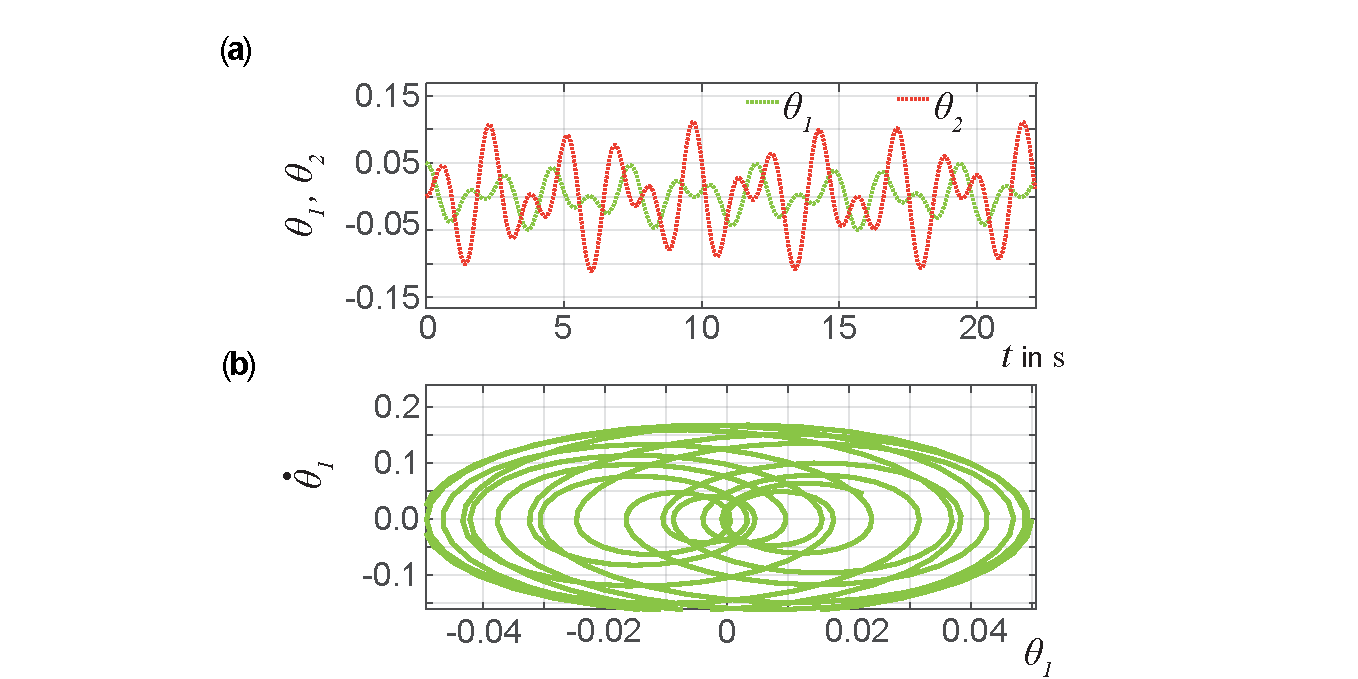
\includegraphics[width=\textwidth]{DoppelPendel03.pdf}%
\caption[Kleinwinkelverhalten des Doppelpendels.]{Kleinwinkelverhalten des Doppelpendels. \fa Bei geringen Auslenkungen zeigt das Doppelpendel mehr oder weniger ein Schwebungsverhalten, \dh die Energie wandert �ber die Zeit zwischen den beiden Pendelarmen hin und her. 
Im Bild ist die analytische N�herung nach \eqref{eq:bew_Doppelpendel07} f�r die entsprechenden Anfangsbedingungen dargestellt.
In der Zeitentwicklung der Auslenkungen der beiden Pendelarme erkennt man das Schwebungsverhalten aus den �berlagerungen der Eigenmoden. 
\fb Der Phasenraum zeigt eine geschlossene Kurve.}\label{abb:bew_Doppelpendel03}
\end{figure}

\subparagraph{\anf{Chaotisches Verhalten} des Doppelpendels}\index{Chaos}

Wir wollen nun das Doppelpendel bei gro�en Auslenkungen $\theta_1, \theta_2$ betrachten,
bei denen es zu chaotischem Verhalten neigt.
Im \mscr{} \mlbewref{Doppelpendel02.m} haben wir die Bewegungsgleichungen f�r das Doppelpendel numerisch mit der \matlab-Routine \odevf gel�st. Die Ergebnisse sind beispielhaft in \figref{bew_Doppelpendel02} dargestellt.
Die numerische L�sung zeigt, dass es au�erhalb des Bereichs, in dem die DGL \emph{linearisiert} wurden, unter bestimmten Bedingungen zu \emph{chaotischem Verhalten}\index{System!chaotisches} kommen kann.
Von \emph{Chaos} spricht man in der Physik, wenn bereits die kleinste �nderung der Anfangsbedingungen zu einem scheinbar v�llig anderen zeitlichen Verhalten f�hrt.%
\footnote{So eine kleine �nderung der Anfangsbedingungen kann \zb auch durch Ungenauigkeiten bei der numerischen Rechnung eintreten. Man mache sich aber klar, dass dies dennoch ein deterministisches Problem ist.}

Allgemein k�nnen wir festhalten, dass f�r chaotisches Verhalten die zugrundeliegenden Lagrange-Funktionen \bzw Bewegungsgleichungen nichtlineare Terme enthalten m�ssen.
Im Falle von \eqref{eq:bew_Doppelpendel02} sind dies die Terme
$\lek \ddot{\theta}_2\,\cos(\theta_2 - \theta_1) - {\dot{\theta}_2}{}^2 \,\sin(\theta_2 - \theta_1)  \rek$ und 
$\lek \ddot{\theta}_1 \,\cos(\theta_2 - \theta_1) - {\dot{\theta}_1}{}^2 \,\sin(\theta_2 - \theta_1)  \rek$
in der Lagrange-Funktion $\mathcal{L}$. 
Das chaotische Verhalten ist im Phasendiagramm $\lek \theta_i(t) \, ~~ \, \dot{\theta}_i(t) \rek$ von \figref{bew_Doppelpendel02} zu erkennen, w�hrend \figref{bew_Doppelpendel03} im Vergleich dazu das Verhalten bei kleineren Auslenkungen $\theta_1, \theta_2$ zeigt und wir hier ein weitgehend \anf{normales} Schwingungsverhalten erkennen.\\
Wir werden das Thema Chaos in \kap{bew_chaos} noch weiter vertiefen.
\begin{figure}
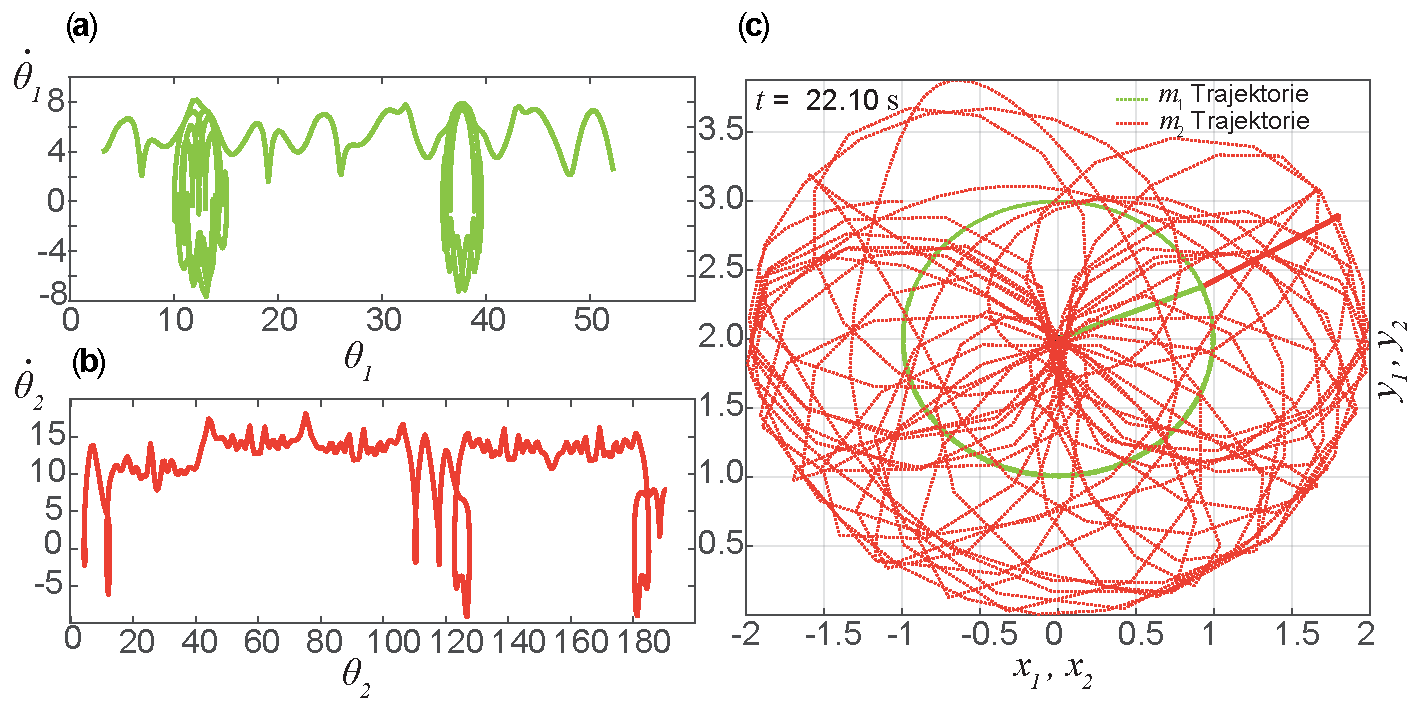
\includegraphics[width=\textwidth]{DoppelPendel02.pdf}%
\caption[Chaotisches Verhalten des Doppelpendels.]{Chaotisches Verhalten des Doppelpendels. \fa, \fb Phasenraum der beiden Pendelarme gezeigt (gr�n = Pendel 1, rot = Pendel 2). Man erkennt, dass es selbst nach l�ngerer Zeit keine geschlossene Kurve gibt, obwohl Energieerhaltung gilt. \fc \gls{traj}n der beiden Pendelarme in kartesischen KoordinatenFrequenzantwort eines Schwingungstilgers (. Die Unstetigkeiten sind durch die Schrittweite in der Darstellung bedingt. Die Zwangsbedingung f�r den Pendelarm 1 ist deutlich zu erkennen. Die Bewegungen der Pendelarme zeigen \anf{chaotisches} Verhalten (\mscr{} \mlbewref{DoppelPendel02.m}).}
\label{abb:bew_Doppelpendel02}
\end{figure}

\subsubsection{Schwingungstilgung}\index{Schwingungstilgung|textbf} \label{kap:bew_Tilgung}

\begin{figure}
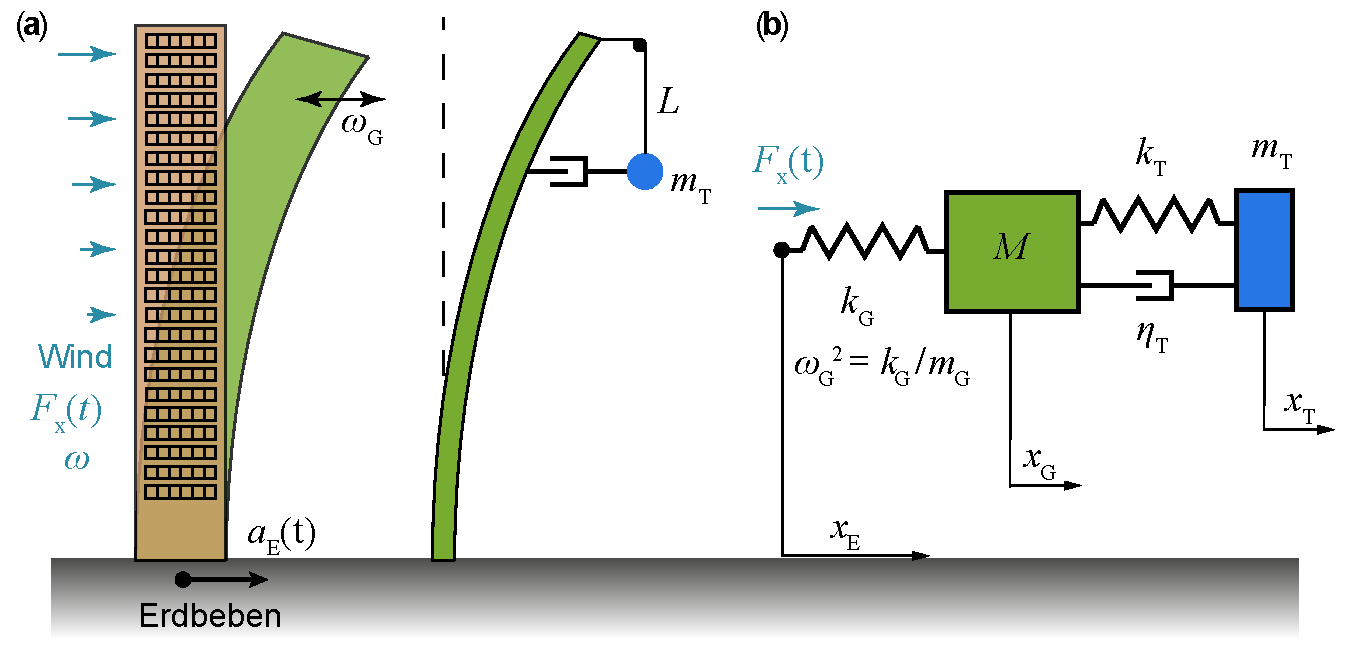
\includegraphics[width=\textwidth]{TilgungSchema.pdf}%
\caption[Schwingungstilgung an Geb�uden.]{Schwingungstilgung an Geb�uden. \fa Anregung durch Wind bzw. Erdbeben \fb Vereinfachtes Modell des Systems.}
\label{abb:bew_TilgungSchema}
\end{figure}

Ein besonders interessanter Fall der Schwingungskopplung sind die sogenannten \emph{Schwingungstilger}. Im Englischen werden diese auch sehr treffend \textit{Tuned Mass Damper} (TMD)\index{Tuned Mass Damper|textbf} oder auch \textit{Tuned Vibration Absorber} (TVA) genannt. Wir werden deshalb auch die Abk�rzung TMD verwenden. Bei diesen Schwingungstilgern wird ein passives Gegengewicht $m_\text{T}$ an eine Hauptmasse $M$ (\zb Geb�ude, Tisch wir benutzen hier zur besseren Unterscheidung den Gro�buchstaben) gekoppelt, deren Schwingungsverhalten bei bestimmten Anregungen unterdr�ckt \bzw ged�mpft werden soll. Es gibt zahlreiche Beispiele f�r solche TMDs, insbesondere bei Hochbauten, so \zb in den USA den John Hancock Tower in Boston, in Deutschland den Berliner Fernsehturm, den Testturm in Rottweil und in Taiwan das Taipei 101 Geb�ude. Die Idee ist, dass bei einer Schwingungsanregung der Hauptmasse, \zb durch Wind, der Tilger die Schwingungsenergie der Hauptmasse aufnimmt und dann d�mpft (\figref{bew_TilgungSchema}a). Dazu muss dieser auf die erwartete externe Anregungs-Schwingungsfrequenz abgestimmt werden. 
Das einfachste physikalische Modell f�r ein solches System zeigt \figref{bew_TilgungSchema}b. Man kann leicht die Lagrange-Funktion $\mathcal{L} = T-U$ und die Dissipationsfunktion aufschreiben und daraus die Bewegungsgleichung herleiten:\footnote{Hier haben wir der Einfachheit halber die D�mpfung der Struktur als klein gegen $\eta_\text{T}$ angenommen und diese wiederum als proportional zur Relativgeschwindigkeit beider Massen, da sich die D�mpfung zwischen den beiden Massen befindet.}
\begin{align}
\begin{split}
    M \,\ddot{x}_\text{M} + \eta_\text{T}\,\lk \dot{x}_\text{M} - \dot{x}_\text{T}\rk + k_\text{M}\,x_\text{M} - k_\text{T}\,\lk x_\text{T} - x_\text{M}\rk &= F_\text{x}\lk t\rk = \hat{F}_\text{x}\,\e_\text{x}^{i\omega t} \,, \\
    m_\text{T}\,\ddot{x}_\text{T} + \eta_\text{T}\,\lk \dot{x}_\text{T} - \dot{x}_\text{M}\rk + k_\text{T}\, \lk x_\text{T} -x_\text{M}\rk &= 0 \,.
\end{split} \label{eq:bew_TilgungBasic01}
\end{align}
Darin sind $M, \eta_\text{M}, k_\text{M}$ durch die Geb�udestruktur vorgegebene Gr��en, ebenso sei $F_\text{x}\lk t\rk$ (\bzw im Frequenzbereich $\hat{F}_\text{x}\lk \omega\rk$) als externe Anregung bekannt.\footnote{Wir lassen erdbeben�hnliche St�rungen unber�cksichtigt, mit anderen Worten das Fundament des Geb�udes bleibt fix ($x_\text{G} = 0,\, a_\text{E} = 0\,.$).} Wir haben diese durch eine komplexe Funktion beschrieben, sodass die L�sungen $x_\text{M}(t), x_\text{T}(t)$ auch komplex werden, und damit neben der Amplitude auch die Phase relativ zur Anregung liefern. Die Frage ist, wie man mit den freien Parametern $m_\text{T}$, $\eta_\text{T}$ und $k_\text{T}$ einen optionalen Tilger (TMD) auslegt. Ziel muss es dabei sein,
\begin{enumerate}
    \item [a)] 
    das Geb�ude/die Struktur (Masse $M$) mit der Eigenfrequenz $\omega_\text{M} = \sqrt{k_\text{M}/M}$ \bzw der externen Anregungsfrequenz $\omega$ optimal zu d�mpfen, \dh die relative Amplitude $x_\text{M}/(F_\text{x}/M)$ so klein wie m�glich zu machen, und
    \item [b)]
    die unweigerlich durch das gekoppelte System zus�tzlich entstehenden Eigenschwingungen mit den Frequenzen $\omega_\text{u}$, $\omega_\text{o}$ so klein wie m�glich und so weit entfernt wie m�glich von $\omega_\text{M}$ auftreten zu lassen. 
\end{enumerate}
Dieses Optimierungsproblem wird zu einem Kompromiss f�hren, da a) und b) gegeneinander \anf{laufen}.
Das kann man sich leicht �berlegen, indem man im DGL-System \eqref{eq:bew_TilgungBasic01} $\,\eta_\text{M} = 0$ und $k_\text{T}/m_\text{T} = k_\text{M}/M = \omega^2$ setzt.
Dann sind die verbleibenden freien Parameter des TMD das Masseverh�ltnis $\gamma= m_\text{T}/M$ und die D�mpfung der Tilgungsmasse $\eta_\text{T}$.
Wir wollen den Einfluss dieser beiden  Parameter auf das Schwingungsverhalten auf Basis der DGL \eqref{eq:bew_TilgungBasic01} berechnen.%
\footnote{In der Literatur finden sich h�ufig leicht verschiedene Bewegungsgleichungen f�r den TMD. Die Unterschiede r�hren vor allem von der unterschiedlichen Verwendung der KOS f�r die beiden bewegten Massen her. Wie haben bei der Herleitung von \eqref{eq:bew_TilgungBasic01} jeweils den $0$-Punkt der Koordinaten in die Ruhelage der Struktur ($x_\text{M}$-Koordinate) \bzw des Tilgers ($x_\text{T}$-Koordinate) gelegt.} \\
Wir sind unter der Annahme einer periodischen Anregung (\zb durch Windb�en) an der station�ren L�sung des gekoppelten Systems interessiert. Dazu machen wir wieder den bereits bekannten Exponentialansatz%
\footnote{Wir k�nnen auch sagen, dass wir das System im Frequenzbereich betrachten und dazu eine Fourier-Transformation der DGL machen. Siehe dazu die \onlineZ \bzw  das Kapitel "`Physik der Musik"' im zweiten Band dieser Reihe, in denen wir uns intensiver mit dem Thema befassen werden.}:
\begin{align}
    x_\text{M} = \hat{X}_\text{M}\,\e^{\im\omega t}\,,~~~ x_\text{T} = \hat{X}_\text{T}\,\e^{\im\omega t} \,. \label{eq:bew_TilgungBasic02}
\end{align}
Das f�hrt auf das folgende lineare Gleichungssystem in $\hat{X}_\text{M}$ und $\hat{X}_\text{T}$:
\begin{align*}
    \hat{X}_\text{M}\,\lk -\omega^2\,M + \im\,\omega\,\eta_\text{M} + k_\text{M} + k_\text{T}\rk + \hat{X}_\text{T}\,\lk -\im\,\omega\,\eta_\text{T} - k_\text{T}\rk &= F_\text{x} \,,\\
    \hat{X}_\text{M}\,\lk -\im\,\omega\,\eta_\text{T} - k_\text{T}\rk + \hat{X}_\text{T}\,\lk -\omega^2\,m_\text{T} + \im\,\omega\,\eta_\text{T} + k_\text{T} \rk &= 0\,.
\end{align*}
Wir l�sen nach $\hat{X}_\text{M}$ und finden
\begin{align}
    \hat{X}_\text{M}(\omega) = \frac{F_\text{x}\lk -\omega^2\,m_\text{T} + \im\,\omega\,\eta_\text{T} + k_\text{T}\rk}{NN} \label{eq:bew_TilgungBasic03} 
\end{align}
mit
\begin{align*}
    NN = \lk -\omega^2\,M + \im\,\omega\,\eta_\text{M} + k_\text{M} + k_\text{T}\rk\lk -\omega^2\,m_\text{T} + \im\,\omega\,\eta_\text{T} + k_\text{T}\rk - \lk \im\,\omega\,\eta_\text{T} + k_\text{T}\rk^2  \; .
\end{align*}
Die sogenannte \gls{frequenzantwort} (Englisch: \textit{Frequency Response} $R\lk\omega\rk$) des Systems auf die Anregung mit der Frequenz $\omega$ ist dann: 
\begin{align}
    R\lk\omega\rk = \frac{k_\text{M}\,\hat{X}_\text{M}\lk\omega\rk}{\hat{F}_\text{x}} \; . \label{eq:bew_TilgungBasic04} 
\end{align}
Diese Frequenzantwort ist eine komplexe Gr��e. Wir sind zun�chst nur an ihrem Betrag interessiert, den wir aus \eqref{eq:bew_TilgungBasic03} numerisch (\mscr{} \mlbewref{Tilgung01.m}) berechnen.\\
%Wir erhalten:
%\begin{align}
%\begin{split}
    %|R\lk \omega\rk|^2 &= R\lk \omega\rk\,R^*\lk\omega\rk \\
    %|R\lk \omega\rk|   &= \frac{1}{c^2+d^2}\,\sqrt{\lk ac+bd\rk^2 + \lk bc-ad\rk^2}~~~\text{mit} \\ 
    %a &= -\omega^2\,m_\text{T} + k_\text{T} \\
    %b &= \omega\,\eta_\text{T} \\
    %c &= \omega^4\,M\,m_\text{T} - \omega^2\,\lk k_\text{M}\,m_\text{T} + k_\text{T}\,m_\text{T}\rk + k_\text{M}\,k_\text{T} \\
    %d &= -\omega^3\,\eta_\text{T}\,\lk M + m_\text{T}\rk - \omega^2\,M\,k_\text{T} + \omega\,\eta_\text{T}\,k_\text{M}
%\end{split} \label{eq:bew_TilgungBasic05} 
%\end{align}
Wir k�nnen uns nun einige Spezialf�lle �berlegen:
\begin{itemize}
    \item $\eta_\text{T} \rightarrow \infty$: Der Tilger ist dann quasi starr an die Struktur gekoppelt, die Eigenfrequenz der Struktur wird sich leicht verschieben zu $\omega_\text{M}{}' = \sqrt{k_\text{M}/\lk M + m_\text{T}\rk}$.
    \item $\eta_\text{T} \rightarrow 0$: In diesem Fall gilt $R\lk \omega\rk = 0$ f�r $\omega = \omega_\text{T} = \sqrt{k_\text{T}/m_\text{T}}$.
\end{itemize}
F�r den Spezialfall $\eta_\text{T} = 0$ zeigt \figref{bew_TilgungBasic01}a die Frequenzantwort f�r verschiedene Massenverh�ltnisse $\gamma= m_\text{T}/M$ und \figref{bew_TilgungBasic01}b die Frequenzantwort f�r verschiedene $\eta_\text{T}$ bei konstantem Massenverh�ltnis $\gamma= 0.05$.
\figref{bew_TilgungBasic02} zeigt die Frequenzantwort $|R\lk\omega\rk|$ f�r verschiedene Abstimmungen (\dh D�mpfungen) eines TMD mit dem Masseverh�ltnis $\gamma = \SI{0.1}{}$ und einer D�mpfung von $\eta_\text{T} = \SI{0.05}{\kg\per\second}$. 

\begin{figure}
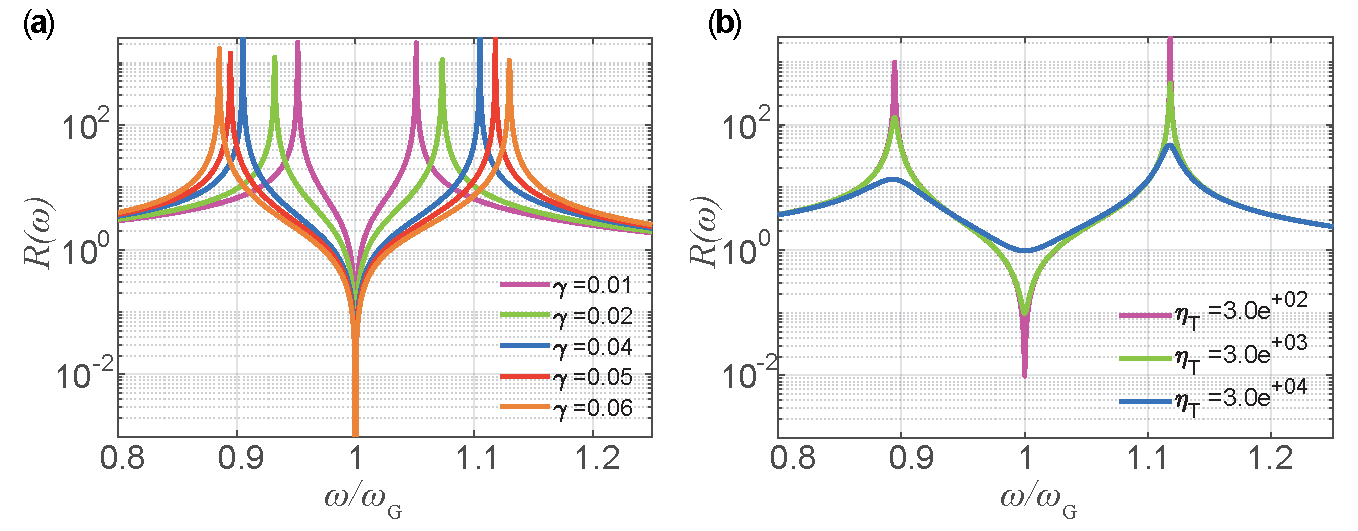
\includegraphics[width=\textwidth]{TilgungBasic01.pdf}%
\caption[Frequenzantwort eines Schwingungstilgers.]{Frequenzantwort eines Schwingungstilgers (TMD) f�r verschiedene Parameter. Linkes Bild: Verschiedene Massenverh�ltnisse $\gamma$ und $\eta_\text{T} = 0$. Rechtes Bild: Verschiedene D�mpfungen $\eta_\text{T}$ in $\SI{}{\kg\per\s}$ und konstantes Massenverh�ltnis $\gamma = 0.05$.}
\label{abb:bew_TilgungBasic01}
\end{figure}

Worin besteht nun eine Optimierung, m.\,a.\,W.\ die richtige \anf{Abstimmung}  \bzw das richtige \anf{Tuning}? Wir verwenden hier das sogenannte \textit{Den Hartog-Verfahren} \cite{DenHartog1984}, dessen Vorgehen in Folgendem besteht:
\begin{enumerate}
    \item
    Man w�hlt ein passendes Masseverh�ltnis $\gamma =  m_\text{T}/M$. Dieses liegt typischerweise im Bereich $0.01 \ldots 0.05$. Man beachte, dass f�r $M$ die effektiv schwingende Masse eingesetzt wird. Die Eigenfrequenz $\omega_\text{M} = \sqrt{k/M}$ sei bekannt. 
    \item
    Man hat nun zwei freie Parameter, mit denen man die Frequenzantwort optimieren kann. N�herungsweise kann man f�r $\gamma < 0.05$ die optimale Eigenfrequenz des Tilgers $\omega_\text{T,opt}$ aus 
			\[\omega_\text{T,opt} \approx \sqrt{\frac{1-0.5\,\gamma}{1+\gamma}}\,\omega_\text{M}
	\]
	bestimmen. 
    \item
	Die optimale D�mpfung des Tilgers findet man bei 
    \begin{align*}
        \eta_\text{T,opt} = 2\,\omega_\text{T,opt}\,m_\text{T} \sqrt{\frac{\gamma\,\lk 3-\sqrt{0.5\,\gamma}\rk }{8\lk 1 +\gamma \rk \lk 1 - 0.5\,\gamma \rk}}\,.
    \end{align*}
\end{enumerate}
Die Frequenzantwort eines nach diesen Kriterien abgestimmten TMD ist ebenfalls in \figref{bew_TilgungBasic02} gezeigt. Wie man sieht, ist im Unterschied zum nicht abgestimmten TMD die Tilgung beim abgestimmten TMD im Bereich der Eigenfrequenz etwas geringer, daf�r \anf{verh�lt} sich aber das System insgesamt �ber einen gr��eren Frequenzbereich hinweg \anf{gutartiger}, \dh die Frequenzantwort ist �ber einen Bereich von etwa $0.9\,\omega_\text{M} - 1.1\,\omega_\text{M}$ relativ konstant. 

\begin{figure}
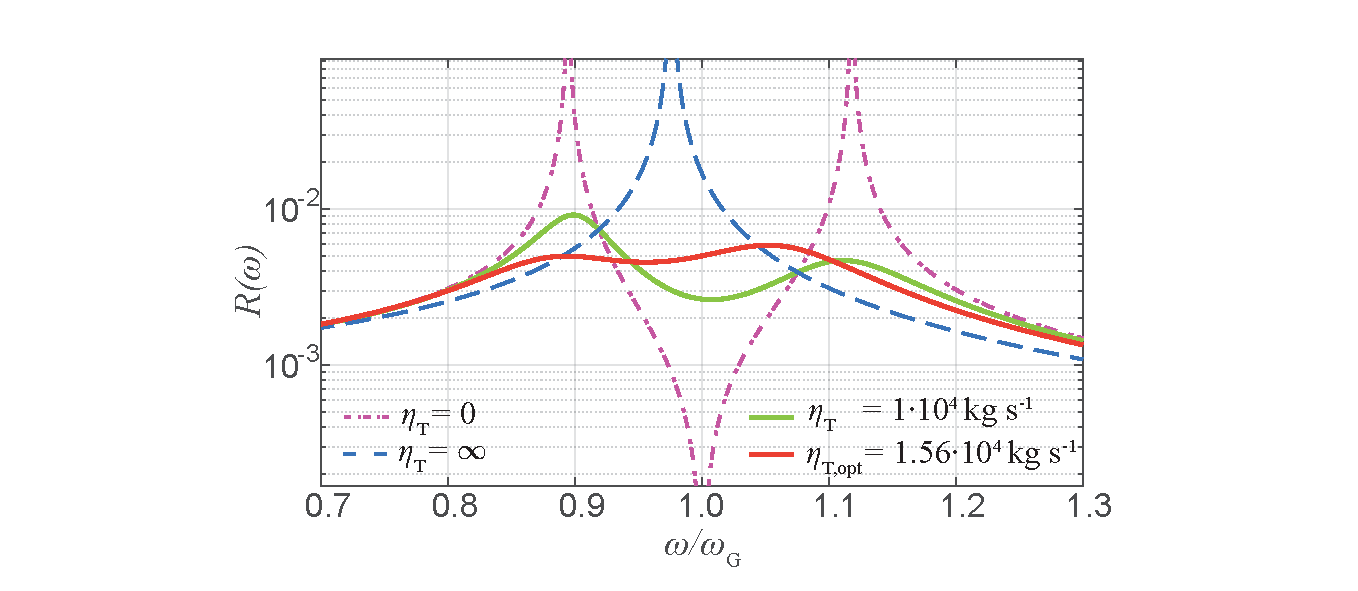
\includegraphics[width=\textwidth]{TilgungBasic02.pdf}%
\caption[Schwingungstilgung nach dem Den Hartog-Verfahren.]{Schwingungstilgung nach dem Den Hartog\footnote{Jacob Pieter Den Hartog (1901--1989) war ein niederl�ndisch-US-amerikanischer Ingenieurwissenschaftler f�r Mechanik, der 1940 die theoretischen Grundlagen f�r mechanische Schwingungstilger aufstellte.}\indexp{Den Hartog, Jacob Pieter}-Verfahren \cite{DenHartog1984}. Die rote durchgezogene Kurve zeigt den abgestimmten Schwingungstilger. }
\label{abb:bew_TilgungBasic02}
\end{figure}

In \probref{bew_Stossdaempfer} wollen wir verschiedene Tilgungssysteme im Detail betrachten und auch die hier dargestellte Methode auf Bauwerke wie das Taipei 101 und den Berliner Fernsehturm anwenden.
Die Erweiterung der dargestellten Methode auf St�rungen durch Erdbeben ist relativ einfach.
Man erweitert die Lagrange-Gleichungen \eqref{eq:bew_TilgungBasic01} um eine dritte generalisierte Koordinate $x_\text{G}$ und ber�cksichtigt die Erdbebenerregung, die an die gro�e Masse $M$ ankoppelt, durch $a_\text{E}$.\\
Wir beenden dieses Kapitel �ber Pendel und Oszillatoren, das uns tiefe Einblicke in viele grundlegende Prinzipien und Methoden der Physik erlaubte,
mit dem Hinweis auf die weiterf�hrenden und vertiefenden �bungen \ref{prob:bew_PendelUeb01} bis \ref{prob:bew_schaukelIII},
sowie ein sehr empfehlenswertes Buch \cite{Matthews2005} mit vielen Literaturhinweisen zu Themen rund um das Pendel.


\subsection{Nichtlinearit�t und Chaos} \index{Nichtlinearit�t}\index{Chaos|textbf} \label{kap:bew_chaos}

Chaos ist ein h�ufig auftretendes Ph�nomen in nichtlinearen Systemen, nicht nur in der Physik \cite{Seifritz1987}.
Wir wollen deshalb einige wichtige Elemente der Chaostheorie behandeln, f�r eine tiefergehende Betrachtung empfehlen wir \cite{Morin2008, Kuypers2012, Mandelbrot2004}.\\
Von Chaos spricht man, wenn eine geringe �nderung der Anfangsbedingungen f�r gro�e Zeiten $t$ zu einem beliebig stark abweichenden Endzustand f�hrt.
Man spricht dann auch vom \anf{Schmetterlingseffekt}.
Der Begriff kommt aus der Klimaforschung und besagt, dass ein kleiner Effekt in einer Region (\zb der Fl�gelschlag des Schmetterlings am Amazonas) einen gro�en Effekt auf das Wetter zu einem viel sp�teren Zeitpunkt und in entfernten Gebieten haben kann, was de facto eine Nicht-Vorhersagbarkeit des Wetters �ber lange Zeiten bedeutet.
Eine mathematisch-physikalische Ursache dieses Ph�nomens ist auch hier die Beschreibung des Systems durch komplexe verkoppelte nichtlineare Differentialgleichungen. \\
Wir wollen als ein einfaches nichtlineares System das getriebene (nichtlineare) Pendel (oder allgemein einen nichtlinearen Oszillator) betrachten.
Die Bewegungsgleichung unter Benutzung der verallgemeinerten Koordinate $q=\theta$ lautet
\begin{align}
    \ddot{q}=-{\omega_0}^2\,\sin q - 2\,\gamma\,\dot{q} + \Gamma\,{\omega_0}^2\,\cos\omega_\text{A}t ~~~~ \text{mit} ~~~~ \Gamma\,{\omega_0}^2 = \frac{F_\text{A}}{m\,l} \,. \label{eq:bew_Chaos01}
\end{align}
Wir k�nnen die Gleichung wieder mit den \matlab-Routinen \odezd \,oder \odeeds\, l�sen und wollen dies f�r verschiedene Anregungs-Parameter und Kopplungst�rken $\Gamma$ tun. \\
Die Anregungsfrequenz ist durch $\omega_\text{A}=2\pi/T_\text{A}$ gegeben und wir nehmen der Einfachheit halber $T_\text{A}=\SI{1}{\second}$ an. 
Die Parameter $\omega_0 = 1.25 \omega_\text{A}$ und $\gamma=\omega_0/5$ (schwache D�mpfung) halten wir konstant, ebenso zun�chst die Anfangsbedingungen $q_0=q(t=0)= \pi/3$ und $\dot{q}_0 = \dot{q}\lk t=0\rk = 0$. \\
Um die Bewegung nach langen Zeiten (also nach einem wie auch immer gearteten Einschwingverhalten) zu charakterisieren, tr�gt man $q$ und $\dot{q}$ f�r lange Zeiten $t \gg T_\text{A}$ auf.
Diese Darstellung nennt man Phasenraum.
Eine besonders n�tzliche Methode, um solche Phasenr�ume f�r nichtlineare, chaotische Systeme zu untersuchen, wurde vom franz�sischen Mathematiker Poincar�\footnote{Henri Poincar�\indexp{Poincar�, Jules Henri} (1854--1912) war ein bedeutender franz�sischer Mathematiker und Physiker und dar�ber hinaus auch Astronom und Philosoph.} entwickelt.
Sie wird nach ihm Poincar�-Schnitt genannt und besteht darin, dass man die Schnittpunkte einer Trajektorie $q\lk t\rk$, $\dot{q}\lk t\rk$ mit einer gedachten Fl�che ($q_P,\,\dot{q}_P$) �r $t \gg T_\text{A}$ ermittelt.
Bei einer geschlossenen Trajektorie im Phasenraum, also f�r eine \glqq normale \grqq{} unged�mpfte bzw. erzwungene Schwingung ist der Poincar�-Schnitt dann genau ein Punkt.
\figref{bew_Chaos01} zeigt das Schwingungsverhalten f�r eine schwache Anregung mit $\Gamma = 1.0$.
Man erkennt, dass die Schwingung nahezu harmonisch ist, der Phasenraum geschlossen und der Poincar�-Schnitt\index{Poincar�-Schnitt} ein einzelner Punkt. \\
\figref{bew_Chaos02} und \figref{bew_Chaos03} zeigen die entsprechenden Graphen f�r gr��ere Werte von $\Gamma$.
F�r $\Gamma=1.24$  zeigen Phasenraum und Poincar�-Schnitt das Vorhandensein von 4 (ann�hernd) geschlossenen Trajektorien an, das System pendelt zwischen vier Zust�nden hin und her, w�hrend im Fall von $\Gamma=1.7$ der Poincar�-Schnitt eine Figur ergibt, die auch als \glqq seltsamer Attraktor\grqq \index{Attraktor} bezeichnet wird.
Sie ist eine Indikation daf�r, dass man das chaotische Regime erreicht hat.
Tr�gt man die Koordinate $q$ des Poincar�-Schnitts �ber $\Gamma$ auf, so sieht man, dass es zun�chst zu sogenannten Bifurkationen, \dh zu Aufspaltungen der Trajektorien kommt, bis bei noch gr��eren $\Gamma$ das Ph�nomen des Chaos einsetzt.
Eine solche Darstellung hei�t auch Bifurkations-Graph und wir wollen diesen f�r einen anderen Fall eines chaotischen Systems in \probref{bew_logisticmap} berechnen.\\

\begin{figure}
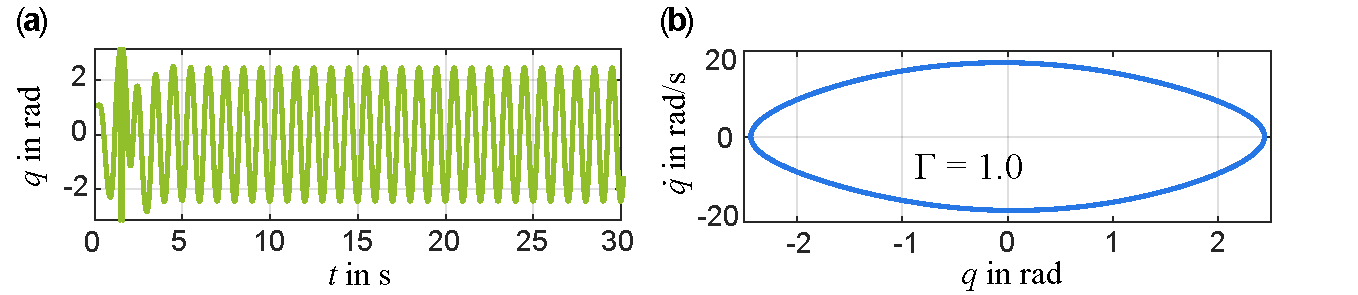
\includegraphics[width=\textwidth]{NLOgamma100.pdf}%
\caption[Verhalten des getriebenen nichtlinearen Oszillators f�r $\Gamma=1.0$.]{\fa Auslenkung des getriebenen nichtlinearen Oszillators f�r $\Gamma=1.0$. \fb Der Phasenraum ergibt eine geschlossene Kurve, der Poincar�-Plot einen Punkt (nicht gezeigt). Die weiteren Parameter: $\omega_\text{A} = 2\pi$, $\omega_0 = 1.25 \omega_\text{A}$ und $\gamma = \omega_0/5$ (\mscr{} \mlbewref{NLOszillator01.m}).}
\label{abb:bew_Chaos01}
\end{figure}

\begin{figure}
\begin{minipage}{\textwidth}
\leftfigure{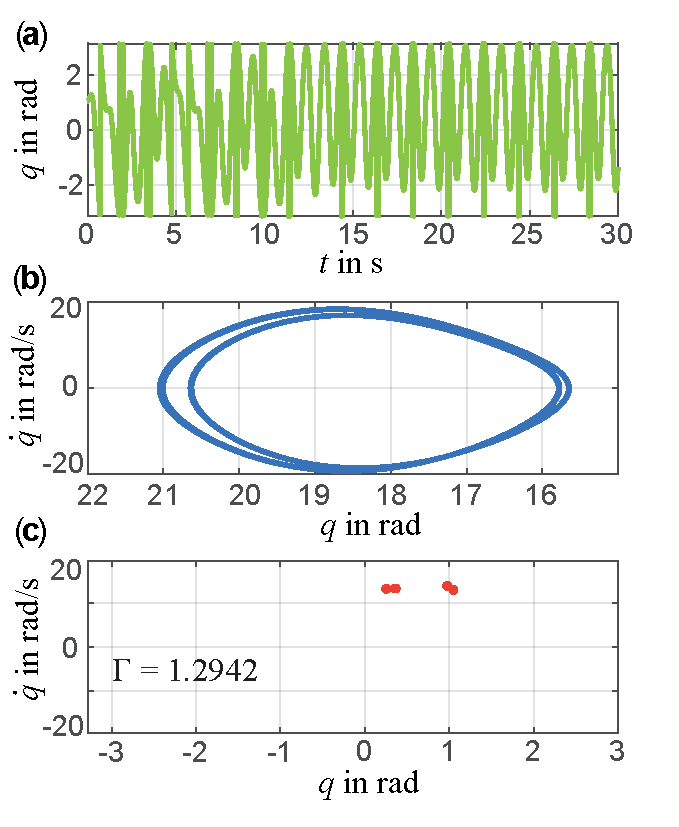
\includegraphics[width=0.5\textwidth]{NLOgamma12942.pdf}}%
\hspace{\fill}
\rightfigure{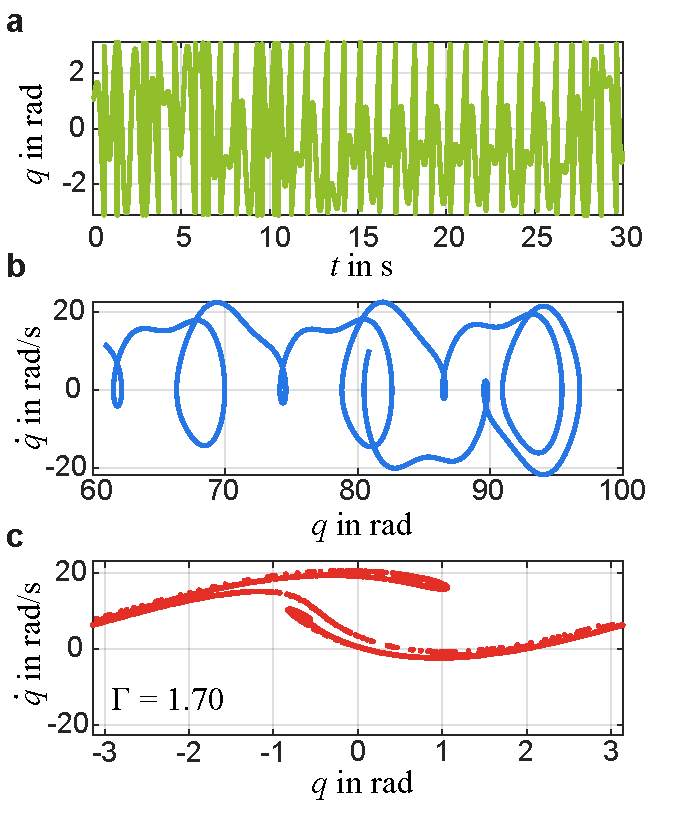
\includegraphics[width=0.5\textwidth]{NLOgamma170.pdf}}
\leftcaption[Verhalten des getriebenen nichtlinearen Oszillators f�r $\Gamma=1.2942$.]{\fa Auslenkung des getriebenen nichtlinearen Oszillators f�r $\Gamma=1.2942$. \fb Der Phasenraum ergibt vier ann�hernd geschlossene Kurven. \fc Der Poincar�-Plot zeigt vier Punkte. Die weiteren Parameter: $\omega_\text{A} = 2\pi\SI{}{\per\s}$, $\omega_0 = 1.25 \omega_\text{A}$ und $\gamma = \omega_0/5$ (\mscr{} \mlbewref{NLOszillator01.m}).}\label{abb:bew_Chaos02}
\rightcaption[Verhalten des getriebenen nichtlinearen Oszillators f�r $\Gamma=1.7$.]{\fa Auslenkung des getriebenen nichtlinearen Oszillators f�r $\Gamma=1.7$. \fb Der Phasenraum ergibt keine geschlossenen Kurven mehr, \fc Poincar�-Plot zeigt den sogenannten seltsamen Attraktor \textit{(Strange Attractor)}.}\label{abb:bew_Chaos03}
\end{minipage}
\end{figure}

Wir wollen jetzt aber noch der Frage nachgehen, wie man erkennen kann, ob bei gegebenen Parametern ein System chaotisches Verhalten zeigt.
Dazu kann man den sogenannten \index{Ljapunow-Exponent|textbf}Ljapunow-Exponenten\footnote{Alexander Michailowitsch Ljapunow\indexp{Ljapunow, Alexander Michailowitsch} (1857--1918) war ein russischer Mathematiker und Physiker, der vor allem auf dem Gebiet der Differentialgleichungen und der Stabilit�t dynamischer Systeme arbeitete.} verwenden, der ein Ma� f�r die Empfindlichkeit des nichtlinearen Systems f�r die Varianz in den Anfangsbedingungen ist.
Ist $\delta_{q0}= q_{01}-q_{02}$ ein Ma� ist f�r eine kleine Abweichung der Anfangsbedingungen, dann wird der Ljapunow-Exponent $\lambda$ nach
\begin{align}
    \Delta_{qt}= q_1\lk t\rk - q_2\lk t\rk = \delta_{q0}\,\e^{\lambda\,t}  \label{eq:bew_Chaos02}
\end{align}
berechnet, worin $\Delta_{qt}$ die Differenz der L�sungen zu einer gro�en Zeit $t$ ist.
Ist $\lambda < 0$, so werden die L�sungen nach langer Zeit konvergieren, f�r $\lambda > 0$ entsprechend divergieren.

\begin{figure}
\begin{minipage}{\textwidth}
\leftfigure{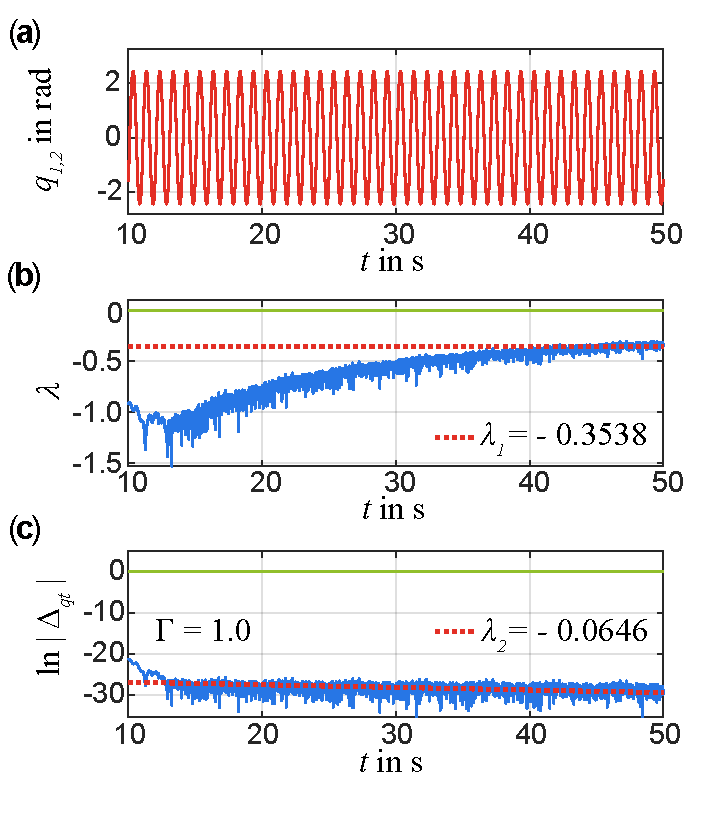
\includegraphics[width=0.5\textwidth]{NLOgammaLjapunow100.pdf}}%
\hspace{\fill}
\rightfigure{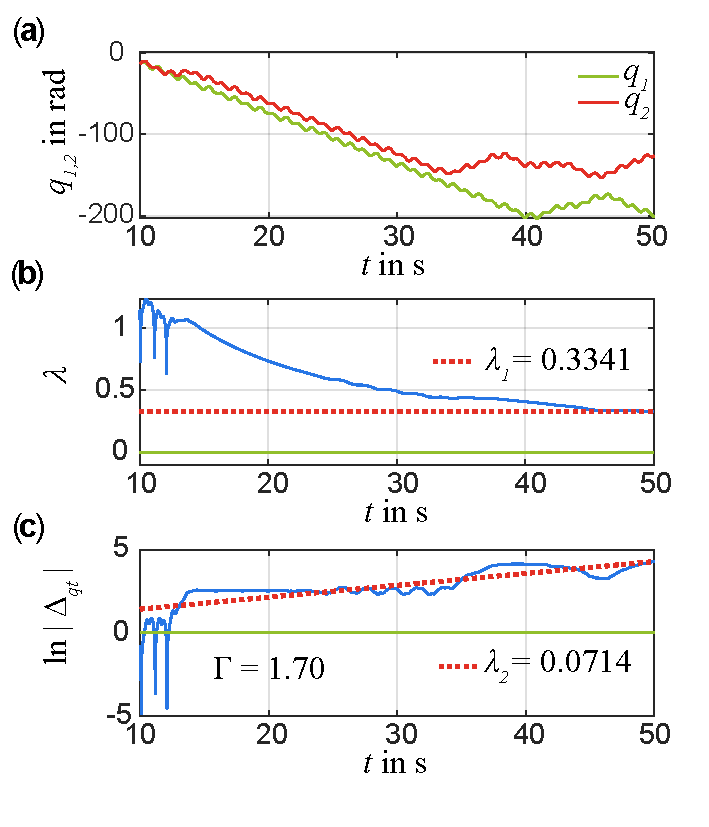
\includegraphics[width=0.5\textwidth]{NLOgammaLjapunow170.pdf}}
\leftcaption[Berechnung des Ljapunow-Exponenten f�r $\Gamma=1.0$.]{\fa Auslenkung und \fb\fc verschiedene Berechnungen des Ljapunow-Exponenten eines getriebenen nichtlinearen Oszillators f�r $\Gamma=1.0$. Die weiteren Parameter: $\omega_\text{A} = 2\pi\SI{}{\per\s}$, $\omega_0 = 1.25 \omega_\text{A}$ und $\gamma = \omega_0/5$ (\mscr{} \mlbewref{NLOszillator01.m}).  Der Ljapunow-Exponent $\lambda$ ist nach beiden Berechnungsmethoden kleiner als Null, das System ist stabil.}\label{abb:bew_Chaos04}
\rightcaption[Berechnung des Ljapunow-Exponenten f�r $\Gamma=1.7$.]{\fa Auslenkung und \fb\fc verschiedene Berechnungen des Ljapunow-Exponenten eines getriebenen nichtlinearen Oszillators f�r $\Gamma=1.7$. Der Ljapunow-Exponent $\lambda$ ist nach beiden Berechnungsmethoden gr��er als Null, das System zeigt chaotisches Verhalten.}\label{abb:bew_Chaos05}
\end{minipage}
\end{figure}

Wie bestimmt man nun den Ljapunow-Exponenten f�r ein nichtlineares dynamisches System wie den getriebenen nichtlinearen Oszillator?
Wir wollen dazu zwei N�herungsmethoden aufzeigen.
Wir berechnen im \mscr{} \mlbewref{NLOszillator02.m} wie f�r \figref{bew_Chaos01} und \figref{bew_Chaos03} die Trajektorien $q\lk t_0\rk$,
diesmal allerdings f�r zwei verschiedene Anfangsbedingungen,
die sich durch $q_{10}-q_{20} = 10^{-6}$ unterscheiden.
Ceteris paribus erhalten wir die Kurven in \figref{bew_Chaos04} und \figref{bew_Chaos05} f�r $q_1\lk t\rk$, $q_2\lk t\rk$ (Abb. a), $\Delta_{qt}$ (Abb. b) und $\ln\,\Delta_{qt}= \ln\,\delta_{q0}+\lambda\,t$ (Abb. c).
Offensichtlich ergibt sich f�r $\Gamma=1$ aus \figref{bew_Chaos04} ein $\lambda < 0$ und f�r $\Gamma = 1.7$ aus \figref{bew_Chaos05} ein $\lambda >0$.
Wir weisen darauf hin, dass diese numerischen Absch�tzungen des Ljapunow-Exponenten nur eine Indikation �ber das eventuell chaotische Verhalten des Systems geben.
In \cite{ Kuypers2012} wird gezeigt, wie man anhand einer Analyse der Differentialgleichung den Ljapunow-Exponenten gewinnen kann.

\subsection{Vermischtes zur Mechanik von Massepunkten und Massepunktsystemen}\label{kap:bew_mixed_mechanics}

\subsubsection{Streu- und Sto�prozesse}\index{Streuung} \label{kap:bew_scatter_problems}

\subparagraph{\textbf{Rutherford-Streuung}}\index{Streuung!Rutherford-}\index{Rutherford-Streuung}

In Kapitel Sto�- und Streuprozesse (\kap{bew_stoss}) haben wir die Formel \eqref{eq:bew_Streuung18} f�r den Wirkungsquerschnitt eines geladenen Teilchens im Coulomb-Feld  als Funktion des Streuwinkels $\vartheta'$ im Schwerpunktsystem (im Englischen oft \textit{Center of Mass}- oder CoM-System genannt)\index{Center of Mass} hergeleitet. Wir haben dabei das Streuzentrum (\zb einen Atomkern) im Laborsystem $\vec{\Sigma}_\text{L}$ als ruhend angenommen:
        \begin{align}
            \frac{\D \sigma'}{\D \Omega'} = \lk \frac{\alpha}{4E}\rk^2\,\frac{1}{\sin^4\,\lk\frac{\vartheta'}{2}\rk}\,. \label{eq:bew_Rutherford_review}
        \end{align}
Wir wollen nun den Wirkungsquerschnitt im Laborsystem berechnen und zwar f�r verschiedene Massenverh�ltnisse von gestreutem Teilchen und Streuzentrum. Wir wollen dabei auch untersuchen, welchen Fehler man macht, wenn man den R�cksto� auf das Streuzentrum nicht ber�cksichtigt. In Gl. \eqref{eq:bew_Rutherford_review} sind im Einzelnen: \\ \\
\begin{tabular}{ll}
   $\alpha = e^2\,Z_\text{Z}\,Z_\text{T}/(4\pi\epsilon_0) ~~~\text{mit}$& \\
	 &\\
   $\epsilon_0 = \SI{8.854e-12}{\ampere\second\per\volt\per\metre}$ &(Dielektrizit�tskonstante),\index{Dielektrizit�tskonstante}\\
   $ e = \SI{1.602e-19}{\ampere\second}$ &(Elementarladung),\index{Elementarladung} \\ 
   $Z_\text{Z} $ &(Kernladungszahl des Streuzentrums),\index{Kernladungszahl}  \\
   $Z_\text{T} $ &(Ladung des gestreuten Teilchens), \\
   $m_\text{Z} = 197 \, \uA $ &(Masse des Streuzentrums-Gold), \\
   $\uA = \SI{1.660539e-27}{\kg} $ &(atomare Masseneinheit),\index{Masseneinheit!atomare} \\
   $E $ & (Energie des Streuteilchens),\\
   $m_\text{eff}= m_\text{Z}\,m_\text{T}/(m_\text{Z} + m_\text{T})$ &(effektive Masse der beiden wechselwirkenden Teilchen). \\ \\
\end{tabular} \\ \\
Mit Gl. \eqref{eq:bew_Streuung7} hatten wir einen Zusammenhang zwischen dem Streuwinkel im Laborsystem $\vartheta_1$ und dem Streuwinkel $\vartheta'$ im Schwerpunktsystem hergeleitet. Wir wollen hier zur besseren Unterscheidung der beiden Winkel den Streuwinkel im Laborsystem mit $\psi = \vartheta_1$ bezeichnen. Bildet man die Ableitung $\D \psi / \D \vartheta'$ von 
\begin{align}
  \psi  = \arctan \lk \frac{\sin\vartheta'}{\cos\vartheta' + \frac{m_T}{m_Z}}  \rk \label{eq:bew_Rutherford00}
\end{align}
 und setzt diese gleich Null, erh�lt man im Fall, dass das Streuzentrum schwerer ist als das gestreute Teilchen (${m_T} \geq {m_Z}$) den maximalen Streuwinkel im Laborsystem zu
\begin{align}
	\tan \psi_\text{max} = \frac{m_\text{T}/m_\text{Z}}{\sqrt{1-\lk m_\text{T}/m_\text{Z} \rk^2}} \,~ \rightarrow ~~ \psi_\text{max} = \arcsin{\frac{m_\text{T}}{m_\text{Z}}}\,. \label{eq:bew_Rutherford01}
\end{align}
F�r ${m_T} = {m_Z}$  betr�gt dieser $90\degree$, es gibt in diesem Fall also keine R�ckstreuung. \\
Wir wollen nun den differentiellen Wirkungsquerschnitt als Funktion des im Laborsystem experimentell bestimmbaren Streuwinkels $\psi$ berechnen. Dazu halten wir fest, dass der Wirkungsquerschnitt im CoM- und im Laborsystem gleich sein muss, was gleichbedeutend ist mit
\begin{align}
      \frac{\D \sigma}{\D \Omega} 2\pi\,\sin\psi \,\D \psi  \stackrel{!}{=} \frac{\D \sigma'}{\D \Omega'} 2\pi\,\sin\vartheta' \,\D \vartheta'\,. \label{eq:bew_Rutherford02}
\end{align}
Hieraus folgt
\begin{align}
	%\frac{\D \sigma(\psi)}{\D \Omega} &= \frac{\D \Omega}{\D \Omega'} \, \frac{\D \sigma(\theta')}{\D \Omega'} \nonumber \\
	\frac{\D \sigma(\psi)}{\D \Omega} &= \frac{\sin\vartheta'(\psi)}{\sin\psi} \,\frac{\D \vartheta'(\psi)}{\D\psi} \frac{\D \sigma(\vartheta')}{\D \Omega'}\,. \label{eq:bew_Rutherford03}
\end{align}
Gl. \eqref{eq:bew_Rutherford03} ergibt relativ komplexe Zusammenh�nge zwischen den beiden differentiellen Streuquerschnitten, wir k�nnen hier vorteilhaft mit \matlab{} numerisch rechnen. Eine einfache analytische L�sung ergibt sich f�r den Spezialfall, bei dem Streuzentrum und gestreutes Teilchen dieselbe Masse haben. Dann ist nach \eqref{eq:bew_Streuung7} $\psi = \vartheta'/2$ und aus \eqref{eq:bew_Rutherford03} folgt
\[\frac{\D \sigma(\psi)}{\D \Omega} = 4\, \cos\psi \frac{\D \sigma(\vartheta')}{\D\Omega'} \,.\]
Im \mscr{} \mlbewref{Rutherford.m} haben wir verschiedene F�lle untersucht: 
\begin{itemize}
\item \textit{Fall 1:\, Gold $_{197}^{79}$Au- und Silber $_{109}^{47}$Ag-Teilchen auf Goldfolie } \\ \\
\begin{tabular}{ll} 
Schwerpunktsystem & Laborsystem mit R�cksto� \\ \\
$m_\text{T} = 197 \uA \,,~m_\text{Z} = 197 \uA,~ E = \SI{1e7}{\electronvolt}~~$& $E_\text{L} = {m_\text{Z} + m_\text{T}}/{m_\text{Z}}\, E = 2 E$\\
$m_\text{T} = 109 \uA \,,~m_\text{Z} = 197 \uA,~ E = \SI{1e6}{\electronvolt}~~$& $E_\text{L} = {m_\text{Z} + m_\text{T}}/{m_\text{Z}}\, E = 1.55 E$  
\end{tabular} \\ \\
\item \textit{Fall 2:\, $_2^4$He-($\alpha$)-Teilchen\index{Alpha-Teilchen@$\alpha$-Teilchen}\index{Alpha-Teilchen} auf Gold- und Silberfolie} \\ \\
\begin{tabular}{ll} 
Schwerpunktsystem & Laborsystem mit R�cksto� \\ \\
$m_\text{T} = 4 \uA \,,~m_\text{Z} = 197 \uA, ~ E = \SI{5e5}{\electronvolt}~~$ & $E_\text{L} = {m_\text{Z} + m_\text{T}}/{m_\text{Z}}\, E = 1.02 E$\\
$m_\text{T} = 4 \uA \,,~m_\text{Z} = 109 \uA, ~ E = \SI{5e5}{\electronvolt}~~$ & $E_\text{L} = {m_\text{Z} + m_\text{T}}/{m_\text{Z}}\, E = 1.04 E$ 
\end{tabular} \\ 
\end{itemize}
Das Ergebnis der Rechnungen ist in \figref{bew_Rutherford01} gezeigt.
\begin{figure}
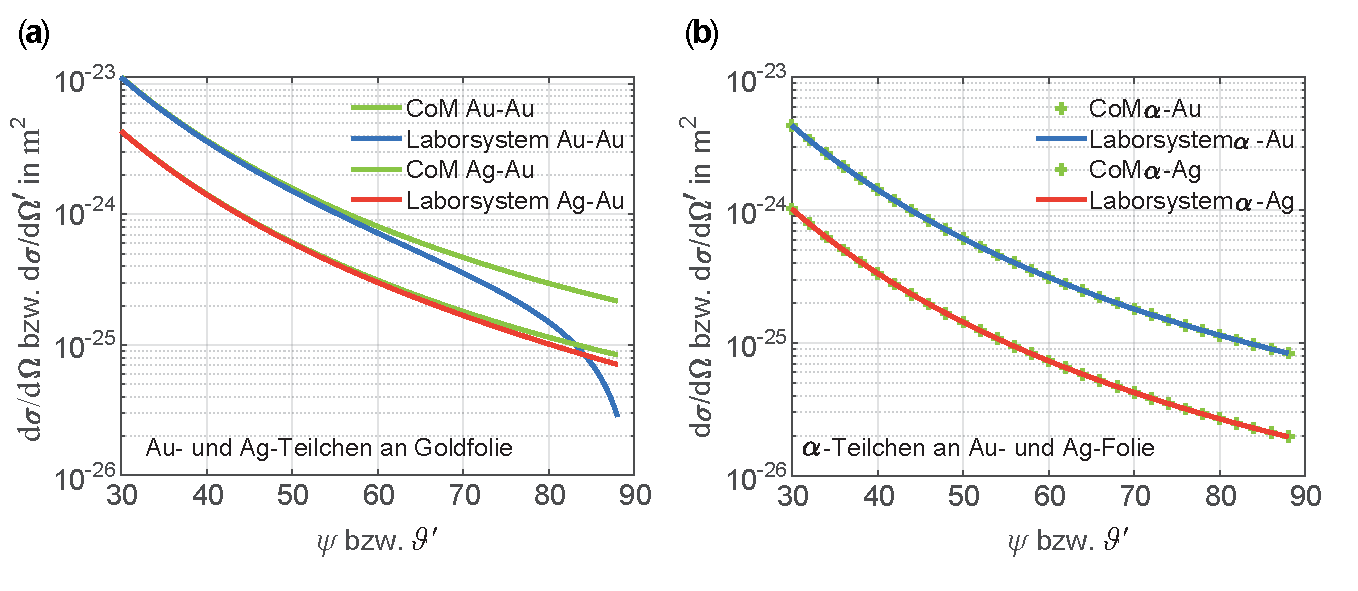
\includegraphics[width=\textwidth]{Rutherford01.pdf}%
\caption[Rutherford-Streuung von Gold- und Silberatomen.]{Rutherford-Streuung von \fa Gold- \bzw Silberatomen, sowie \fb $\alpha$-Teilchen jeweils an einer Goldfolie. CoM steht f�r Betrachtung im Schwerpunktsystem (\textit{Center of Mass}).}
\label{abb:bew_Rutherford01}
\end{figure}

Im Vergleich der Bilder a) und b) erkennt man sehr sch�n,
dass im Experiment von 1913 \cite{Geiger1913} zur Rutherford-Streuung
die Benutzung der Formel f�r das CoM System \eqref{eq:bew_Streuung19} gerechtfertigt war,
da $m_\text{T} \ll m_\text{Z}$.
Bei vergleichbaren Massen von Streuzentrum und Streuteilchen
wie \zb im Fall des Beschusses der Goldfolie mit hochenergetischen Gold- oder Silberteilchen
ist die N�herung aber nicht mehr gerechtfertigt. \\
In \probref{bew_Rutherford} und in den \mscren \mlbewref{RutherfordAlpha.m} \bzw \mlbewref{RutherfordAg.m} zeigen wir, wie man das Streuproblem durch numerische Integration der Bewegungsgleichungen f�r verschiedene Einfallstrajektorien (Sto�parameter $b$) simulieren und l�sen kann.

\subparagraph{\textbf{Asteroidenbahnen}}

Wir wollen noch darauf hinweisen, dass auch die Bewegung nicht geschlossener Asteroidenbahnen (oder Bahnen anderer Himmelsk�rper) als Streuproblem nach dem Rutherford-Modell betrachtet werden kann, da das Gravitationspotential ja dieselbe Struktur hat wie das Coulomb-Potential. Man setzt einfach in \eqref{eq:bew_Rutherford_review} $\alpha = G\,m_\text{A}\,m_\text{E}$ (mit $m_\text{A}$ als Masse des Asteroiden und $,m_\text{E}$ als Masse der Erde) und kann dann alle Formeln entsprechend verwenden. \\
Wir wollen vereinfachend annehmen, dass sich die beiden wechselwirkenden K�rper in der $x$-$y$-Ebene bewegen, die gleichzeitig die Ebene der Mondbahn und der Erde sein soll. Das ist 
ein Zweik�rperproblem Erde-Asteroid (\figref{bew_asteroid}) mit folgenden (etwas willk�rlich) angenommenen Parametern.\footnote{So ganz willk�rlich sind die Parameter nicht. Am 15.\ Februar 2013 kam der Asteroid 367943 Duende der Erde bis auf \SI{27.599}{\kilo\metre} nahe, was innerhalb der Umlaufbahn der geostation�ren Satelliten lag. Der Asteroid war sogar mit blo�em Auge zu erkennen (\url{https://www.nasa.gov/topics/solarsystem/features/asteroidflyby.html}\, Durch Einfl�sse von Erde und Mond wurde seine Bahn um die Sonne signifikant ver�ndert. So verk�rzte sich \zb seine Umlaufperiode um die Sonne von 336 auf 317 Tage.\cite{JPL2020}}:
\begin{align*}
    v_\infty &=  \SI{4}{\km\per\s} && \text{Geschwindigkeit relativ zur Erde vor der Begegnung}\,, \\
    b &= \SI{25000}{\km} && \text{Sto�parameter}, \\
    \epsilon &= 1.004 && \text{Exzentrizit�t und} \\
    \varphi &= \arccos \lk -\frac{1}{\epsilon}\rk \approx 175\degree && \text{�ffnungswinkel, sowie} \\
    r_\text{min} & \approx \SI{10700}{\km} \,.
\end{align*}

\begin{figure}
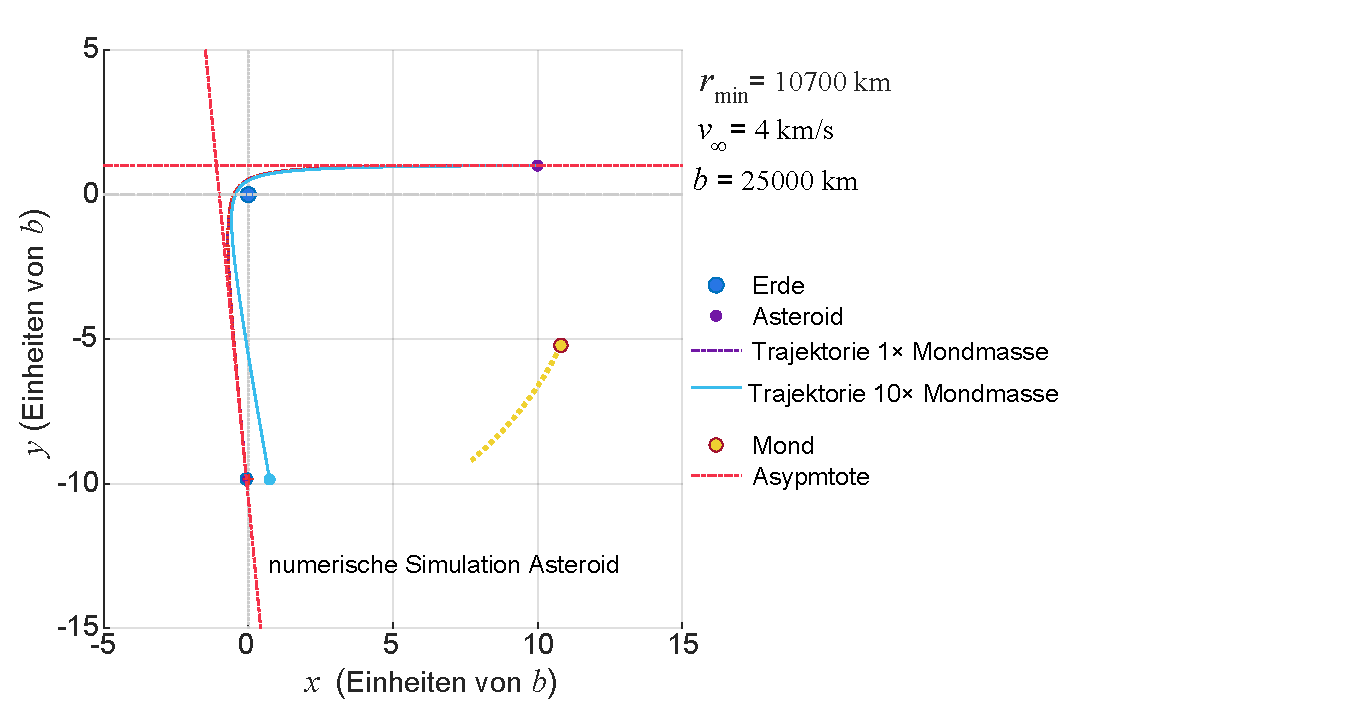
\includegraphics[width=\textwidth]{Asteroid.pdf}%
\caption[Streuung eines Asteroiden im Gravitationsfeld von Erde und Mond.]{Streuung eines Asteroiden im Gravitationsfeld von Erde und Mond (vereinfachte Annahmen). Im Bild wird die Streuung durch den Mond in sogenannter Oppositionsstellung zum Asteroiden und im Vergleich dazu bei Annahme eines Mondes mit zehnfach gr��erer Masse gezeigt.}
\label{abb:bew_asteroid}
\end{figure}

Wenn wir die Erde als ruhend in (0,0) annehmen, wird das Ganze 
mit $m_\text{E} \gg m_\text{A}$ dann
ein einfaches Streuproblem.
Wir k�nnten die L�sung dieses Streuproblems entweder nach der Hyperbell�sung von \kapitel{bew_ZKP_NZKF} oder auch als Streuproblem nach \kap{bew_stoss} darstellen:
Wir wollen hier aber die Trajektorie des Asteroiden numerisch
berechnen und dabei untersuchen, was passiert, wenn 
wir den Mond in unsere Betrachtungen einschlie�en.
Wir nehmen vereinfachend an, dass dieser sich mit konstanter
Umlaufgeschwindigkeit auf einer Kreisbahn um die Erde bewegt
und die Position der Erde sich nicht ver�ndert
(was nicht ganz korrekt ist, siehe Himmelsmechanik im Band II, Kapitel 3).
Der Asteroid bewegt sich dann in einem zeitlich ver�nderlichen
Gravitationspotential, seine Bewegungsgleichung lautet%
\footnote{Man kann das Problem auch als Streuung an einem
zeitlich ver�nderlichen \bzw bewegten Streuzentrum verstehen.}
\begin{align}
    m_\text{A}\,\ddot{\vec{ r}}_\text{A} = - m_\text{A}\,G\,\lek \frac{ m_\text{E}}{|\vec{r}_\text{A}|^2} + \frac{ m_\text{M}}{|\vec{r}_\text{A}-\vec{r}_\text{M}|^2}\rek ~~ \label{eq:bew_asteroid01a}\\
		\text{mit} ~~ \vec{r}_\text{M} = 		\begin{pmatrix} x_\text{M}\\ y_\text{M} \end{pmatrix} =
  \begin{pmatrix}
      R_\text{ME}\,\cos\omega_\text{M}t + \varphi_0\\
      R_\text{ME}\,\sin\omega_\text{M}t + \varphi_0
  \end{pmatrix} \,. \label{eq:bew_asteroid01b}
\end{align}
Wir wollen Gl. \eqref{eq:bew_asteroid01a} numerisch integrieren und erhalten mit $\vec{r}_\text{A} = \begin{Bmatrix} x\\ y \end{Bmatrix}$
\begin{align}
    \ddot{\vec{x}} &= \begin{pmatrix} \ddot{x} \\ \ddot{y} \end{pmatrix} = - \frac{G\,m_\text{E}} {\lk x^2+y^2 \rk^{3/2}} \begin{Bmatrix} x\\ y \end{Bmatrix} -\frac{G\,m_\text{M}}{\lk x-x_\text{M}\rk^2 + \lk y-y_\text{M}\rk^2} \begin{Bmatrix} x-x_\text{M}\\ y-y_\text{M} \end{Bmatrix} \\ \label{eq:bew_asteroid02}
    & \text{mit} \nonumber \\
    R_\text{ME} &= \SI{384000}{\km}~~\text{und}~~ \omega_\text{M}  = \sqrt{\frac{G\,\lk m_\text{E} + m_\text{M} \rk}{R_\text{ME}^3}} \approx \SI{2.6e-06}{\per\second}\,.
\end{align}

Die numerische Integration von \eqref{eq:bew_asteroid02} haben wir im \mscr{} \mlbewref{Asteroid.m} ausgef�hrt und das Ergebnis ist in \figref{bew_asteroid} zu sehen: Es zeigt, dass der Mond einen geringen, aber doch messbaren Einfluss auf die Streuung und damit die Bahn des Asteroiden hatte. In ung�nstigerer Konstellation k�nnte der Mond durchaus einen ansonsten an der Erde vorbeifliegenden Asteroiden so abenken, dass er auf der Erde aufschl�gt. 


\subsubsection{Fallschirmsprung} \index{Fall!freier}\index{Fallschirmsprung}\label{kap:bew_parachute}

Das Fallschirmspringen hat eine erstaunlich lange Tradition:
Schon im alten China sprangen im 14.\ Jahrhundert Menschen mit Fallschirmen von T�rmen.
In Europa hat Leonardo da Vinci%
\footnote{Leonardo da Vinci (1452--1519) war eines der gro�en Universalgenies der Renaissance,
er war bildender K�nstler, Architekt, Anatom, Ingenieur und Naturphilosoph.
Besonders seine vielen mechanischen Konstruktionen, von denen aber nicht alle funktionierten,
haben die Menschen begeistert.}
in heute noch erhaltenen Originalzeichnungen Fallschirmspringer festgehalten
(\url{http://www.museoscienza.org}). \\
Am 14.~Oktober~2012 sprang der �sterreicher Felix Baumgartner
aus $\SI{39}{\km}$ H�he aus einem Ballon und erreichte im freien
Fall eine Maximalgeschwindigkeit von $\SI{1342}{\km\per\hour}$.
Er war damit der erste Mensch, der ohne zus�tzlichen Antrieb
die sogenannte Schallmauer durchbrach.%
\footnote{Ohne zus�tzlichen Antrieb ist wohl auch etwas untertrieben,
immerhin kostete die Unternehmung ca.\ 50 Millionen USD.}
Wir wollen diesen Rekord zum Anlass nehmen und die Dynamik des freien Falls aus gro�er H�he untersuchen.
Dabei wollen wir uns auch der Frage widmen, auf welche H�he man mindestens steigen muss, um im freien Fall �berschallgeschwindigkeit zu erreichen. 
Wir modellieren den Sprung von Baumgartner in vier Phasen \cite{Corvo2019}:
\begin{itemize}
    \item [A] -- freier Fall (in gro�er H�he)
    \item [B] -- freier Fall in mittlerer H�he und Vorbereitung f�r Schirm�ffnung
    \item [C] -- Schirm�ffnung 
    \item [D] -- finale Phase mit Schirm
\end{itemize}

\subparagraph{\textbf{Phase A -- Absprung bis Schirm�ffnung}}

Die Bewegungsgleichung f�r die H�he $z$ �ber der Erdoberfl�che in Phase A lautet 
        \begin{align}
            \ddot{z} = -g + \eta\,{\dot{z}}^2 = -g + \hat{\eta}_0\,\rho(z)\,{\dot{z}}^2 = -g + \hat{\eta}_0\,\varrho_0\,\e^{-\kappa\,z}\,{\dot{z}}^2 = -g + \eta_0\,\e^{-\kappa\,z}\,{\dot{z}}^2\,. \label{eq:bew_skydive01}
        \end{align}
Hierin ist $\eta$ der Widerstandskoeffizient, dessen Abh�ngigkeit von $z$ wir hier mithilfe der \emph{barometrischen H�henformel}\glslink{baroHoeheBew} (siehe \probref{kontmech_BarometrischeHoehenformel}) modelliert haben.\index{H�henformel!barometrische}
Prinzipiell k�nnte der Widerstandskoeffizient auch von der Geschwindigkeit abh�ngen, aber dies wollen wir hier der Einfachheit halber vernachl�ssigen.
Wir verwenden die Werte
 \begin{align*}
    \varrho_0 &=\SI{1.225}{\kg\per\cubic\metre}\,,~~~\kappa = \frac{\tilde{M}_\text{L}\,g}{k_\text{B}\,T}\,,~~~ \hat{\eta}_0 = \frac{1}{2\,m}\,A\,c_\text{W}\,,
  \end{align*}
worin $\tilde{M}_\text{L} = \SI{28.9e-3}{\kg\per\mole}$ die molare Masse der Luft, $T$ die absolute Temperatur und $k_\text{B} = \SI{1.381e-23}{\J\per\K\per\mole}$ die Boltzmann-Konstante sind. 
Offensichtlich ist der Widerstandskoeffizient wegen \eqref{eq:bew_skydive01} in gro�en H�hen deutlich geringer.%
\footnote{Da $\kappa$ von der Temperatur und diese ihrerseits von der H�he abh�ngt, gilt streng genommen $\kappa(z)\approx \frac{1}{T(z)}$.
Wir wollen aber zun�chst $\kappa = \con$ mit einer mittleren Temperatur annehmen.} \\
Im freien Fall in einem Medium mit Reibung wird eine Endgeschwindigkeit $v_\text{final}$ erreicht.
Wir nehmen an, dass die Schwerebeschleunigung konstant ist, \dh $g\lk z\rk = g = \con$ und erhalten
\begin{align}
    v_\text{final}\lk z\rk = \sqrt{\frac{2m\,g}{A\,c_\text{W}\,\varrho \lk z\rk}}\,. \label{eq:bew_skydive03}
\end{align}
In der N�he des Erdbodens gilt
$v_\text{final}\lk 0\rk = v_\text{final, 0} = \sqrt{\frac{2m\,g}{\varrho_0\,A\,c_\text{W}}}$, sodass 
\begin{align}
    \frac{v_\text{final}\lk z\rk}{v_\text{final, 0}} = \sqrt{\frac{\varrho_0}{\varrho\lk z\rk}} \label{eq:bew_skydive04}
\end{align}
ist. 
Wir wollen nun wissen, von welcher H�he aus man mindestens springen muss, um die Schallgeschwindigkeit $v_\text{S}$\index{Schallgeschwindigkeit} zu erreichen.
Wir setzen also $v_\text{final}\lk z\rk = v_\text{S}$ und erhalten aus \eqref{eq:bew_skydive04} und \eqref{eq:bew_skydive03} f�r die minimale atmosph�rische H�he, in der durch freien Fall Schallgeschwindigkeit erreicht werden kann
    \begin{align}
        z_\text{min}' = 2\,\ln\lk \frac{v_\text{S}}{v_\text{final, 0}}\rk \,\frac{1}{\kappa}\,.\label{eq:bew_skydive04a}
    \end{align}
Dazu muss man mindestens noch die Fallstrecke 
    \begin{align*}
        z_\text{fall} = \frac{1}{2}\,\frac{{v_\text{S}}^2}{g} 
    \end{align*}
addieren, die (bei Vernachl�ssigung der Reibung) durchlaufen werden muss,
um die Schallgeschwindigkeit%
\footnote{Auch die Schallgeschwindigkeit h�ngt von $v_\text{S}$ ab,
sodass \eqref{eq:bew_skydive04a} eigentlich eine transzendente Gleichung wird:
$\ln v_\text{S}(z_\text{min}') = \ln v_\text{final,0}+(1/2)\,\kappa\,z_\text{min}'$.}
zu erreichen, sodass wir schlie�lich
        \begin{align}
            z_\text{min} \geq {z_\text{min}}'+z_\text{fall} \approx \SI{30}{\km}\label{eq:bew_skydive05}
        \end{align}
erhalten.
Wir haben dabei $v_\text{final, 0} \approx \SI{80}{\metre\per\second}$, $\kappa \approx \SI{0.125}{\per\km}$ und $v_\text{S} \approx \SI{330}{\metre\per\second}$ angenommen.
Man sieht also, dass tats�chlich eine sehr gro�e Anfangsh�he von mehr als $\SI{30}{\km}$ notwendig ist, um Schallgeschwindigkeit im freien Fall zu erreichen. \\
Wir wollen jetzt noch Bewegungsgleichung \eqref{eq:bew_skydive01} l�sen.
Durch die Substitutionen 
	\[v^2 = \dot{z}^2 = u ~~~\text{und}~~~\ddot{z} = \frac{\D z}{\D t}\frac{\D \dot{z}}{\D z} = v\,\frac{\D v}{\D z}
	\]
k�nnen wir diese auf die Form 
\begin{align}
    \frac{\D u}{\D z}-2\eta_0\,e^{-\kappa\,z}\,u =-2g \label{eq:bew_skydive06}
\end{align}
bringen. 
Das entspricht einer DGL des Typs
\begin{align}
    \frac{\D u}{\D z}+A\lk z\rk\, u = B\lk z\rk, \label{eq:bew_skydive07}
\end{align}
deren allgemeine L�sung durch
\begin{align}
    u\lk z\rk = \frac{\int B\lk z'\rk\,\text{exp}\lek\int A\lk z''\rk\,\D z''\rek\,\D z'}{\text{exp}\lek\int A\lk z' \rk \D z'\rek} 
    \label{eq:bew_skydive08}
\end{align}
gegeben ist \cite{Andrews2003, Felder2016}.
Mit der Substitution $q = \frac{2\eta_0}{\kappa}\,\text{exp}\lk -\kappa z\rk$ kann \eqref{eq:bew_skydive08} unter Nutzung des sogenannten \textit{exponentiellen Integrals}\index{Integral!exponentielles} \cite{Gradshteyn1980}
\begin{align*}
    \textbf{Ei}\lk q\rk = \int\limits_{-\infty}^q \,\frac{\text{exp}\lk z'\rk}{z'} \,\D z'
\end{align*}
in die L�sung 
\begin{align}
    v\lk q\lk z\rk\rk = \sqrt{u} = \sqrt{\frac{2g}{\kappa}\,e^{-q}\,\lek \textbf{Ei}\lk q\rk + C\rek}  \label{eq:bew_skydive08A}
\end{align}
gebracht werden, worin $C$ eine Integrationskonstante ist, die durch $v(0)=v_0$ bei $z(0)=z_0$ festgelegt wird. 
Bei einer Anfangsgeschwindigkeit von $v_0=0$ gilt
	\[ C = - \textbf{Ei}\lk q(z_0) \rk = - \textbf{Ei}\lk \frac{2\eta_0}{\kappa}\,e^{-\kappa\,z}\rk \,.
\]

\begin{figure}
\begin{minipage}{\textwidth}
\leftfigure{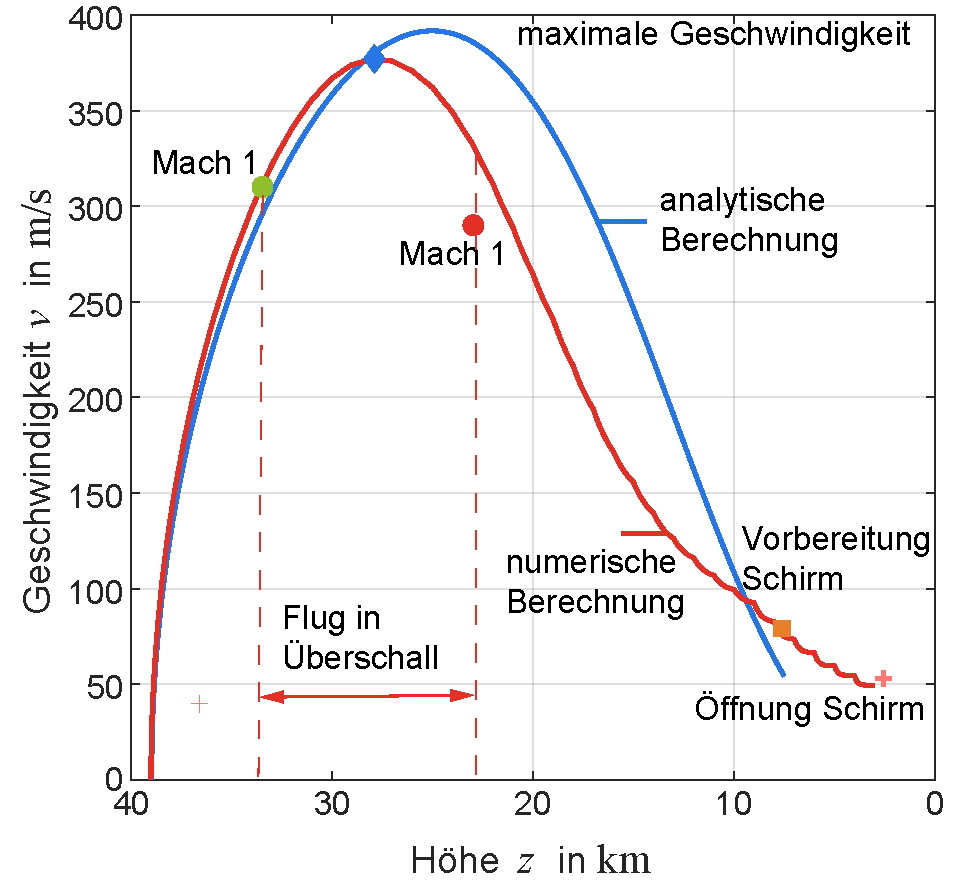
\includegraphics[width=0.5\textwidth]{BaumgartnerFall.pdf}}%
\hspace{\fill}
\rightfigure{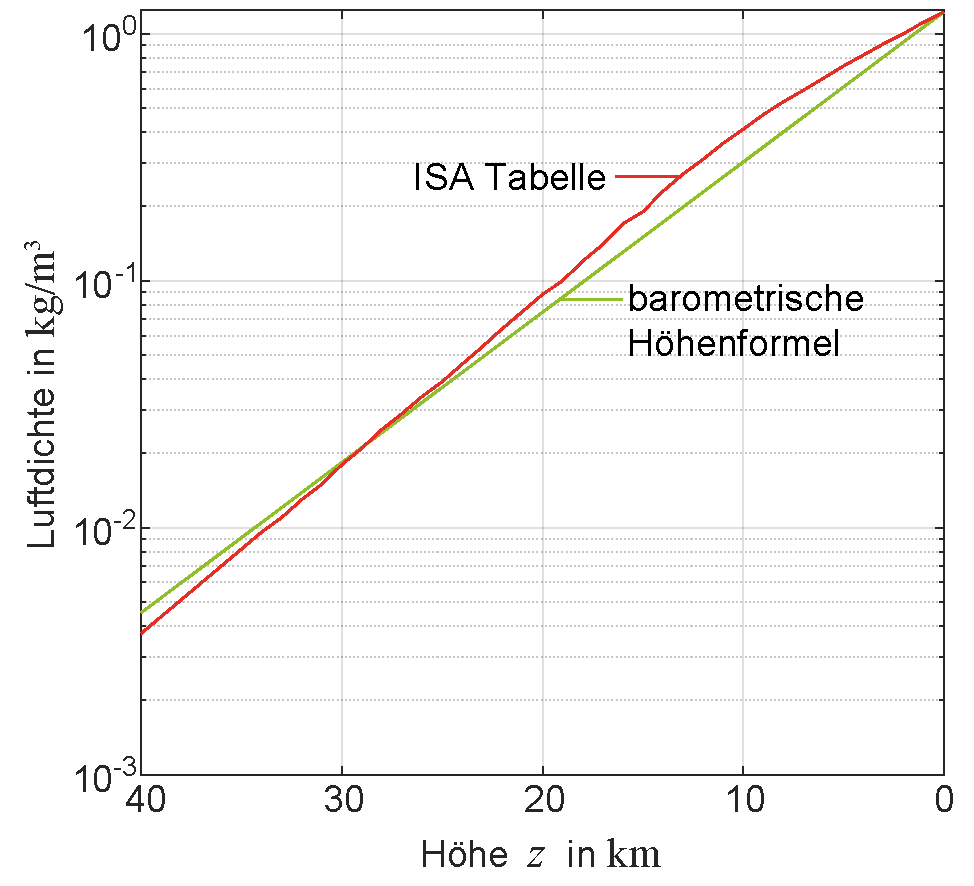
\includegraphics[width=0.5\textwidth]{BaromHoehe.pdf}}
\leftcaption[Fall mit �berschallgeschwindigkeit von Felix Baumgartner.]{Fall mit �berschallgeschwindigkeit von Felix Baumgartner \cite{Corvo2019}. Geschwindigkeit-H�henkurve. Dargestellt sind die Messwerte (einzelne Punkte), die N�herungsberechnung nach der barometrischen H�henformel und die numerische Berechnung nach den tabellierten Werten. Mach 1 bedeutet Erreichen \bzw Unterschreiten der Schallgeschwindigkeit $v_\text{s}$.}\label{abb:bew_BaumgartnerFall}
\rightcaption[Dichteabh�ngigkeit der Atmosph�re nach barometrischer H�henformel.]{Dichteabh�ngigkeit der Atmosph�re nach der barometrischen H�henformel und nach der Standardtabelle \cite{ISA1976}.}\label{abb:bew_BaromHoehe}
\end{minipage}
\end{figure}

In \figref{bew_BaumgartnerFall} haben wir L�sung \eqref{eq:bew_skydive08A} dargestellt.
Wir haben dabei den Wert f�r die Starth�he $z_0 = \SI{38969}{\metre}$
aus \cite{Corvo2019} �bernommen und f�r $\kappa$ einen Mittelwert von
$\kappa \approx \SI{1.4e-4}{}$ als Fit an die barometrische H�henformel angenommen.
Wie wir im Vergleich zu den experimentellen Werten sehen, gibt es eine gute, aber keine perfekte �bereinstimmung (siehe auch \cite{Corvo2019}).
In einigen H�henbereichen gibt es gr��ere Abweichungen.
Neben der N�herung, die wir mit der barometrischen H�henformel gemacht haben,
muss man auch davon ausgehen, dass der $c_\text{w}$-Wert
nicht �ber den gesamten Fallbereich konstant ist, zum einen da der Springer
zu Beginn sicher die senkrechte Lage (Kopf nach unten) eingenommen hat,
um auf Geschwindigkeit zu kommen. Ab ca.~$\SI{10000}{\metre}$ H�he wird er aber
eher die horizontale Lage (Bauch nach unten) einnehmen, um den Fall abzubremsen,
bevor der Schirm ge�ffnet wird.
Ferner ist der $c_\text{w}$-Wert auch im Bereich von Geschwindigkeiten, die im Ultraschalbereich liegen, deutlich unterschiedlich,
siehe \autoref{chap:kontmech}.\\
Wir wollen deswegen die DGL \eqref{eq:bew_skydive01} st�ckweise integrieren, wobei wir die Werte f�r $\varrho\lk z \rk$ aus der US Standard Atmosphere Table \cite{ISA1976} benutzen (siehe \figref{bew_BaromHoehe}). 
Tab.\ \ref{tab:bew_BaumgartnerFall}  und auch die so berechnete Kurve $v(z)$ in \figref{bew_BaumgartnerFall} zeigen eine deutlich bessere �bereinstimmung mit den experimentellen Werten.

\begin{table}[h!]
  \centering
  \begin{tabular}{|C{20mm}|C{15mm}|C{15mm}|C{15mm}|C{15mm}|C{15mm}|C{15mm}|}
  \hline
  \rule{0pt}{3pt}& & & & & &   \\
    & H�he \linebreak exper.\linebreak\linebreak  $\SI{}{\metre}$  & $v$ \linebreak exper.\linebreak \linebreak $\SI{}{\metre\per\second}$ & Zeit \linebreak exper.\linebreak \linebreak $\SI{}{\second}$ & H�he \linebreak Gl. \eqref{eq:bew_skydive08A} \linebreak\linebreak  $\SI{}{\metre}$  & H�he \linebreak Gl. \eqref{eq:bew_skydive01}\linebreak \linebreak  $\SI{}{\metre} $& Zeit \linebreak Gl. \eqref{eq:bew_skydive01} \linebreak \linebreak $\SI{}{\second}$\\
  \rule{0pt}{3pt}& & & & & &  \\
  \hline
  \rule{0pt}{3pt}& & & & & &  \\
  \rule{0pt}{6pt} ~Start   & $\SI{38969}{}$ & $\SI{0}{}$ & $\SI{0}{}$ & $\SI{0}{}$ & $\SI{0}{}$ &  $\SI{0}{}$  \\
  \rule{0pt}{6pt} ~Mach 1   & $\SI{33446}{}$ & $\SI{310}{}$ & $\SI{34}{}$ & $\SI{32669}{}$ & $\SI{33446}{}$ &  $\SI{33}{}$  \\
  \rule{0pt}{6pt} ~Max $v$   & $\SI{27883}{}$ & $\SI{377}{}$ & $\SI{50}{}$ & $\SI{25360}{}$ & $\SI{27883}{}$ &  $\SI{51}{}$  \\
  \rule{0pt}{6pt} ~Mach 1   & $\SI{22961}{}$ & $\SI{290}{}$ & $\SI{64}{}$ & $\SI{17200}{}$ & $\SI{21785}{}$ &  $\SI{69}{}$  \\
  \rule{0pt}{3pt}& & & & & &  \\
  \rule{0pt}{6pt} ~Schirmvorber. & $\SI{7619}{}$ & $\SI{79}{}$ & $\SI{180}{}$ & $\SI{7563}{}$ & $\SI{7438}{}$ &  $\SI{170}{}$  \\
  \rule{0pt}{6pt} ~Schirm�ffnung  & $\SI{2567}{}$ & $\SI{53}{}$ & $\SI{260}{}$ &  &  & \\
  \rule{0pt}{3pt}& & & & & &   \\
  \hline
  \end{tabular}
  \caption[Baumgartner Fall mit �berschallgeschwindigkeit.]{Baumgartner Fall mit �berschallgeschwindigkeit.} \label{tab:bew_BaumgartnerFall}
\end{table}

Mach 1 bedeutet Erreichen \bzw Unterschreiten der Schallgeschwindigkeit $v_\text{s}$, die wir aus \cite{ISA1976} f�r die entsprechende H�he entnommen haben.
Wir wollen jetzt noch kurz die Phase des �ffnens und der Landung mit realistischen Werten betrachten.\\

\subparagraph{\textbf{Phase B -- Landung mit Schirm}}

Der Schirm wird bei $z \approx \SI{2500}{\metre}$ ge�ffnet. Die Entfaltung des Schirms dauert ca.~$\SI{5}{\second}$ (angenommen), der Schirm erzeugt dabei eine Bremsbeschleunigung von bis ca.~$\SI{4}{\g}$, hat also in dieser Phase eine Reibungskraft von 
\begin{align*}
    F_\text{R}\lk z\rk = \frac{1}{2}\,c_\text{w}\,\varrho\lk z\rk\,A\,v^2\lk z\rk\,~~\text{mit}~~c_\text{w} = \SI{1.15}{}\,.
\end{align*}
Die Fl�che steigt in der �ffnungszeit kontinuierlich (n�herungsweise linear) im Laufe von $\SI{5}{\second}$
von ca.~$\SI{1}{\square\metre}$ auf $\SI{50}{\square\metre}$ an, $\varrho\lk z\rk$ k�nnen wir als w�hrenddessen konstant annehmen.
In dieser Phase ab $z = \SI{2500}{\metre}$ muss man also zun�chst eine kontinuierlich ansteigende Bremsverz�gerung
bis zur vollen �ffnung des Schirms in DGL \eqref{eq:bew_skydive01} annehmen.
Wir empfehlen die numerische Rechnung als \probref{bew_SkyDiver}.

Obwohl die Flugphase ab �ffnen des Schirms recht einfach erscheint,
ist deren Berechnung durchaus kritisch.
Kurz vor der �ffnung des Schirms hat der Springer eine Geschwindigkeit von $50 \ldots 60\, \SI{}{\metre\per\second}$, die man auch aus folgender Absch�tzung erh�lt:
        \begin{align*}
            \frac{1}{2}\,\varrho_\text{L}\,c_\text{w}\,A^{(0)}\,{{v_\infty}^{\lk 0\rk}}^2 &= m\,g ~~ \rightarrow ~~{v_\infty}^{\lk 0\rk} = \sqrt{\frac{m\,g}{\frac{1}{2}\,\varrho_\text{L}\,{c_\text{w}}^{\lk 0 \rk}\,A^{\lk 0 \rk}  }} \,.
        \end{align*}
Hierin sind die Werte ${c_\text{w}}^{\lk 0 \rk}$ und $A^{\lk 0 \rk} $ die Werte ohne Schirm, also ${c_\text{w}}^{\lk 0 \rk} \approx 0.3$ und $A^{\lk 0 \rk} \approx 2.53\,\SI{}{\square\metre} $.
Nach dem �ffnen des Schirms ist ${c_\text{w}}^{\lk \text{S} \rk} \approx 0.9 \ldots 1.2$ und $A^{\lk \text{S}\rk} \approx 50 \ldots 60\,\SI{}{\square\metre} $, \dh die Bremskraft steigt um das $60$- bis $80$-Fache an. Die Endgeschwindigkeit reduziert sich um
        \begin{align*}
            {v_\infty}^{\lk \text{S} \rk} \approx \sqrt{\frac{{c_\text{w}}^{\lk 0 \rk}\,A^{\lk 0 \rk}}{{c_\text{w}}^{\lk \text{S} \rk}\,A^{\lk \text{S} \rk}}}\,{v_\infty}^{\lk 0 \rk} \approx \sqrt{4\cdot20}\,{v_\infty}^{\lk 0 \rk} \approx 9\,{v_\infty}^{\lk 0 \rk}\,,
        \end{align*}
also ca.\ um das Neunfache, was in der Tat dann Landegeschwindigkeiten von ca.~$\SI{6}{\metre\per\second}$ ergibt, die in etwa einem Sprung von einer $\SI{1.5}{\metre}$ hohen Mauer entsprechen. 

Die Design-Problematik der �ffnungsphase besteht darin, eine �ffnungszeit des Fallschirms zu finden, die den sogenannten �ffnungsschock vermeidet. Man kann leicht ausrechnen, dass zur Vermeidung einer Belastung von mehr als $4\, g$ die �ffnungszeit $\Delta T$ des Fallschirms bei einer linearen �ffnungsfunktion von $c_\text{w}(t) \, A(t)$ mindestens $\SI{3}{\second}$ betragen muss. In der Realit�t wird man eher nichtlineare Zeitprofile w�hlen (am Anfang langsam, dann schnell) um die �ffnungszeit insgesamt zu minimieren. 

Zum Schluss geben wir der Vollst�ndigkeit halber noch die L�sung des freien Falls\index{Fall!freier} f�r niedrige H�hen, \dh bei konstanter Luftdichte an. In diesem Fall gilt:
        \begin{align}
            \ddot{z} &= -g+\beta\,\dot{z}^2\,,\\
            \frac{\D v_\text{z}}{\D t} = \dot{v}_\text{z} &= -g+\beta\,{v_\text{z}}^2~~\rightarrow ~~\frac{\D v}{-g+\beta\,v^2} &= \D t ~~~~ \text{mit} ~~~~ \beta = \frac{1}{2}\,\varrho_\text{L}\,c_\text{w}\,\frac{A}{m} \,. \label{eq:bew_Fall_exakt01}
        \end{align}
Integration \cite{Gradshteyn1980} ergibt: 
        \begin{align}
            t+C = \frac{1}{\sqrt{g\,\beta}}\frac{1}{2}\ln \lek \frac{1+v\frac{\beta}{g}}{1-v\frac{\beta}{g}} \rek= \frac{\artanh\sqrt{\frac{\beta}{g}\,v}}{\sqrt{g\,\beta}} \,. \label{eq:bew_Fall_exakt02}
        \end{align}
Mit $v\lk 0 \rk  = v_0$ und $\sqrt{g\,\beta} = g/v_\infty$ bestimmt man
        \begin{align}
            C &= \artanh \lk \frac{v_0}{v_\infty}\rk~~\rightarrow ~~v\lk t\rk &= -v_\infty\,\tanh \lk \frac{g\,t}{v_\infty}-\artanh \lk\frac{v_0}{v_\infty}\rk\rk\,. \label{eq:bew_Fall_exakt03}
        \end{align}
Nochmalige Integration \cite{Gradshteyn1980} ergibt
        \begin{align}
            z\lk t\rk = -\frac{v_\infty}{g}\,\ln \lek \sqrt{1-\frac{{v_0}^2}{{v_\infty}^2}}\cosh\,\lek \frac{g\,t}{v_\infty}-\artanh \lk \frac{v_0}{v_\infty}\rk\rek\rek +h_0  \,, \label{eq:bew_Fall_exakt04}
        \end{align}
was sich f�r $v_0=0$ vereinfacht zu
\begin{align}
    z\lk t\rk = h_0 -\frac{{v_\infty}^2}{g}\,\ln\lek \cosh\,\frac{g\,t}{v_\infty}\rek ~~~~ \text{und} ~~~~ v\lk t\rk = -v_\infty\,\tanh\,\frac{g\,t}{v_\infty}\,. \label{eq:bew_Fall_exakt05}   
\end{align}
%Gl. \eqref{eq:bew_Fall_exakt04} \bzw \eqref{eq:bew_Fall_exakt05} sind gut als �berpr�fung f�r die Genauigkeit numerischer Routinen in \matlab{} geeignet.


\subsubsection{Vergl�hen eines Meteoroiden}\index{Meteorit}\index{Meteoroid}

Die Ergebnisse des vorherigen Kapitels k�nnen wir noch auf den Fall anwenden, dass ein kugelf�rmiger Meteoroid\footnote{Hier sei bemerkt, dass \textit{Meteoroid} und \textit{Meteorit} oft verwechselt werden. Ein Meteorit ist ein Himmelsk�rper, der den Erdboden erreicht hat, ein Meteoroid dagegen ein kleines Objekt im Sonnensystem.} der Masse $m$ und des Radius $R$ in die Erdatmosph�re eindringt, durch die Luftreibung abgebremst und schlie�lich auseinandergerissen wird und vergl�ht. Wir wollen �berschalleffekte und auch die Erw�rmung der Luft durch den Meteoroiden vernachl�ssigen, ber�cksichtigen aber die Zunahme der Erdbeschleunigung mit abnehmender H�he:
        \begin{align*}
            g\lk z\rk = -g_0\lk \frac{R_\text{E}}{R_\text{E}+z}\rk^2\,.
        \end{align*}   
Unter Benutzung der barometrischen H�henformel erhalten wir die DGL
        \begin{align}
            \ddot{z} -\frac{1}{2m}\,\varrho_0\,c_\text{w}\,\pi\,R^2\,e^{-\kappa\,z}\,\dot{z}^2 + g_0\lk \frac{R_\text{E}}{R_\text{E}+z}\rk^2 = 0 ~~~~ \text{mit} ~~~~ m = \frac{4}{3}\,\pi\,\varrho_0\,R^3 \,.\label{eq:bew_Meteoroid}
        \end{align}
Wir l�sen \eqref{eq:bew_Meteoroid} numerisch und erhalten f�r Radien von $R = \SI{1}{\mm}$ bis $R = \SI{25}{\mm}$ und eine Dichte von $\SI{7.9}{\kg\per\cubic\metre}$ (Eisen) bei Anfangsgeschwindigkeiten von $15$, $30$ \bzw $\SI{45}{\km\per\second}$ die in \figref{bew_Meteoroid} dargestellten Geschwindigkeitsverl�ufe. \\
Man erkennt, dass ein Meteoroid bestimmter Gr��e immer in etwa derselben H�he abgebremst wird und dabei Bremsbeschleunigungen von bis zu $\SI{100}{\g}$ erf�hrt, die ihn im Allgemeinen zerrei�en und vergl�hen lassen. Das sind dann genau die beobachtbaren \anf{Sternschnuppen}.

\begin{figure}
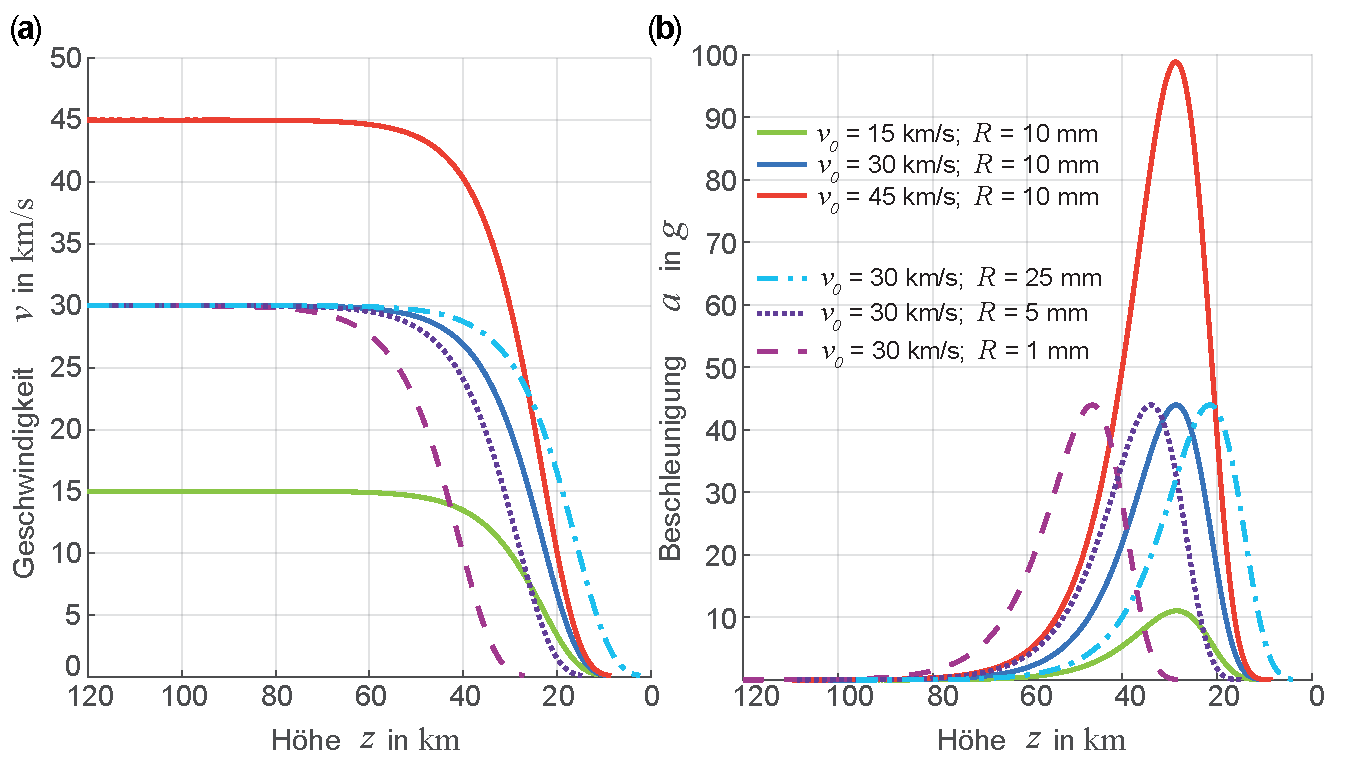
\includegraphics[width=\textwidth]{Meteoroid.pdf}
\caption[Abbremsung eines Meteoroiden in der Erdatmosph�re.]{\fa Geschwindigkeit und \fb Beschleunigung eines Meteoroiden in der Erdatmosph�re. Interessant ist, dass bei �hnlichem Durchmesser die Abbremsung stets in �hnlicher H�he erfolgt. Kleinere/gr��ere Massen/Durchmesser verschieben die H�he zu h�heren/niedrigeren Werten. Bei Anfangsgeschwindigkeiten von $\SI{45}{\km\per\second}$ ergeben sich Bremsverz�gerungen von bis zu $100\,g$.}\label{abb:bew_Meteoroid}
\end{figure}

\subsubsection{Achterbahn} \label{kap:rollercoaster}

Achterbahnen (\figref{bew_Achterbahn01}a), wie generell die Schaustelleranlagen auf den Jahrm�rkten, bieten ein reichhaltiges Angebot f�r physikalische Finger�bungen.\footnote{Achterbahnen sind nicht nur dankbare Studienobjekte f�r die Mechanik. Da Achterbahnz�ge mehrere Tonnen wiegen und Geschwindigkeiten deutlich �ber $\SI{100}{\km\per\hour}$ erreichen, kommen besondere Brems- und Beschleunigungssysteme zum Einsatz. Im der Elektrodynamik werden wir die Physik von Wirbelstrombremsen und linearen Induktionsmotoren behandeln, die beide auf Achterbahnen zum Einsatz kommen.} So ist es nicht verwunderlich, dass es dazu bereits eine Vielzahl von B�chern auf allgemein verst�ndlicher Basis (\zb \cite{Pendrill2021, Weisenberger2013, DPG2012}) gibt.

\begin{figure}
  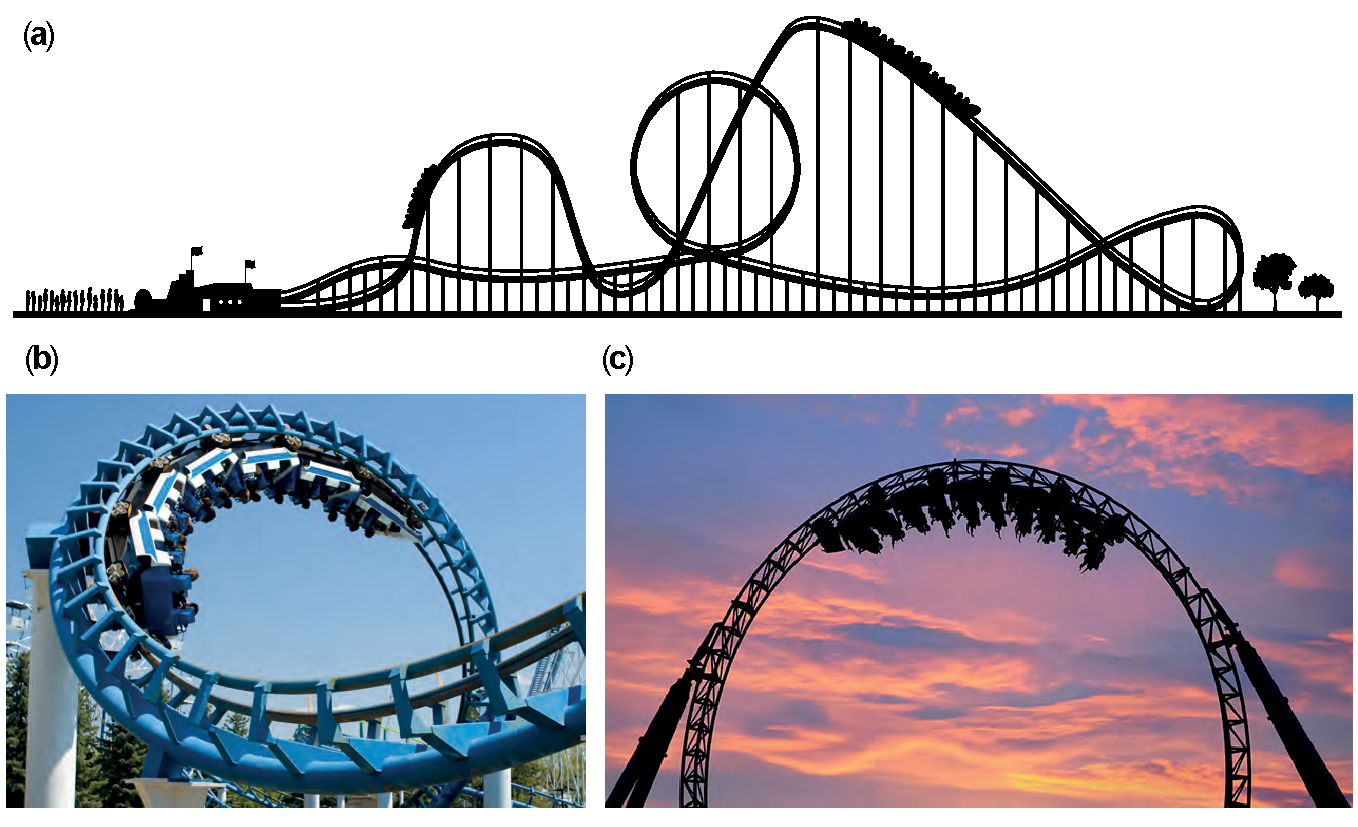
\includegraphics[width=0.95\textwidth]{Achterbahn01.pdf}
  \caption[Typischen Verl�ufe von Achterbahnen mit Looping-Elementen.]{Typischen Verl�ufe von Achterbahnen mit Looping-Elementen. \fa Schema eines typischen Verlaufes. \fb,~\fc Loopings.} \label{abb:bew_Achterbahn01}
\end{figure}

Wer schon mal eine Achterbahn gefahren ist, der hat gesp�rt, wie gro� die Kr�fte sind, die dabei wirken. Sie machen den eigentlichen Nervenkitzel bei den Abfahrten und Loopings erst aus. So kann w�hrend der Fahrt die Beschleunigung des Wagens genauso gro� werden wie die Beschleunigung eines K�rpers im freien Fall. Der Mitfahrer kann dann sein eigenes Gewicht nicht mehr sp�ren und f�hlt sich kurzzeitig in der Luft (auch "`\textit{Airtime}"' genannt) und quasi schwerelos. Die Erkl�rung daf�r kann relativ einfach mit der Newtonschen Mechanik im mitbewegten Koordinatensystem gegeben werden.\\
F�hrt der Wagen durch ein Tal oder eine Kurve, wird die Bewegungsrichtung durch die von den Schienen ausge�bte Zwangskraft auf eine bogenf�rmige Bahn gelenkt. Als Folge dessen sp�rt der Passagier eine Zentrifugalkraft. Im Tal wirken Zentrifugalkraft und Gravitation in dieselbe Richtung. Der Fahrgast f�hlt sich abh�ngig von Kurvenradius \bzw -kr�mmung und Geschwindigkeit deutlich schwerer als sonst. F�hrt der Wagen �ber einen Berg, wirkt die Zentrifugalbeschleunigung vom Wagen weg. Falls diese betragsm��ig gr��er als die Erdbeschleunigung $g$ wird, wird der Mitfahrer nur noch durch einen Gurt im Wagen gehalten.\\
Bei einem Looping (\figref{bew_Achterbahn01}b,c) durchf�hrt der Wagen eine Schleife und befindet sich f�r eine bestimmte Zeit �ber Kopf. Die Zentrifugalkraft im h�chsten Punkt des Loopings muss dann mindestens so gro� sein wie die Gewichtskraft.\\
Mit diesem Wissen k�nnen wir nun sehr einfach berechnen, wie gro� die Geschwindigkeit sein muss, die ein Wagen haben muss, der ein kreisf�rmiges Looping mit Radius $R$ durchf�hrt. Wir werden das f�r einfache F�lle der Achterbahn (Kreisbahn) auf Basis der Newtonschen Mechanik tun. Die Berechnung f�r beliebige Kurvenformen und Zugl�ngen ist mathematisch etwas aufwendiger und wir wollen uns in \probref{bew_achterbahn} etwas grunds�tzlicher mit der Physik auf beliebig gekr�mmten Kurven besch�ftigen und besonders vertieft auch Z�ge in Achterbahnen betrachten. Dabei wollen wir in der �bung auch den Lagrange-Formalismus erster Art \index{Lagrange-Gleichung!Erster Art} benutzen. 

\subparagraph{\textbf{Einzelner Wagen im kreisf�rmigen Looping}}

Wir beginnen die Betrachtung mit einem einzelnen Wagen, der eine kreisf�rmiges Looping fahren soll. Den Wagen betrachten wir als Massepunkt.
Am oberen Punkt des Loopings muss die Zentrifugalkraft gleich der Gewichtskraft sein:
\begin{align*}
    \frac{m\,v_\text{F}{}^2}{R} = m\,g ~~ \rightarrow ~~ v_\text{F}{}^2 = g\,R
\end{align*}
Andererseits muss die Anfangsgeschwindigkeit $v_0$ am Boden gro� genug sein, damit der Massepunkt die H�he $ H = 2R$ erreichen und dann noch eine Geschwindigkeit von $v_\text{F}$ hat, \dh 
\begin{align}
    \frac{m}{2}\,v_0{}^2 &= 2\,m\,g\,R + \frac{m}{2}\,v_\text{F}{}^2 ~~\rightarrow ~~ \frac{v_0{}^2}{2} =  2\,g\,R + \frac{1}{2}\,g\,R ~~\rightarrow~~v_0 = \sqrt{5\,g\,R} \label{eq:bew_Achterbahn01}
\end{align}
Wird der Wagen von einer H�he $H_0$ gestartet, muss diese wegen $2\,g\,H_0 = v_0{}^2$ also mindestens $H_0 = \frac{5}{2}\,R$ betragen. \\

Die Situation ist etwas komplexer, wenn man die Reibung ber�cksichtigt und gleichzeitig eine Einfahrt in das kreisf�rmige Looping nach \figref{bew_loop2loop} betrachtet. Dieses Problem wird in der (angels�chsischen) Literatur als \textit{Loop-the-Loop}-Problem bezeichnet.\index{Loop-the-Loop-Problem}. Am Einfahrtspunkt~T wird der Wagen (Massepunkt) bzw. der im rechten Bild gezeigte rollende Ball eine instantan auftretende Radialbeschleunigung zum Mittelpunkt der Kreisschleife hin erfahren, welche der Mitfahrer als starken \textit{Ruck} (englisch \textit{Jerk})\index{Ruck}\index{Jerk} empfinden w�rde. 

\begin{figure}
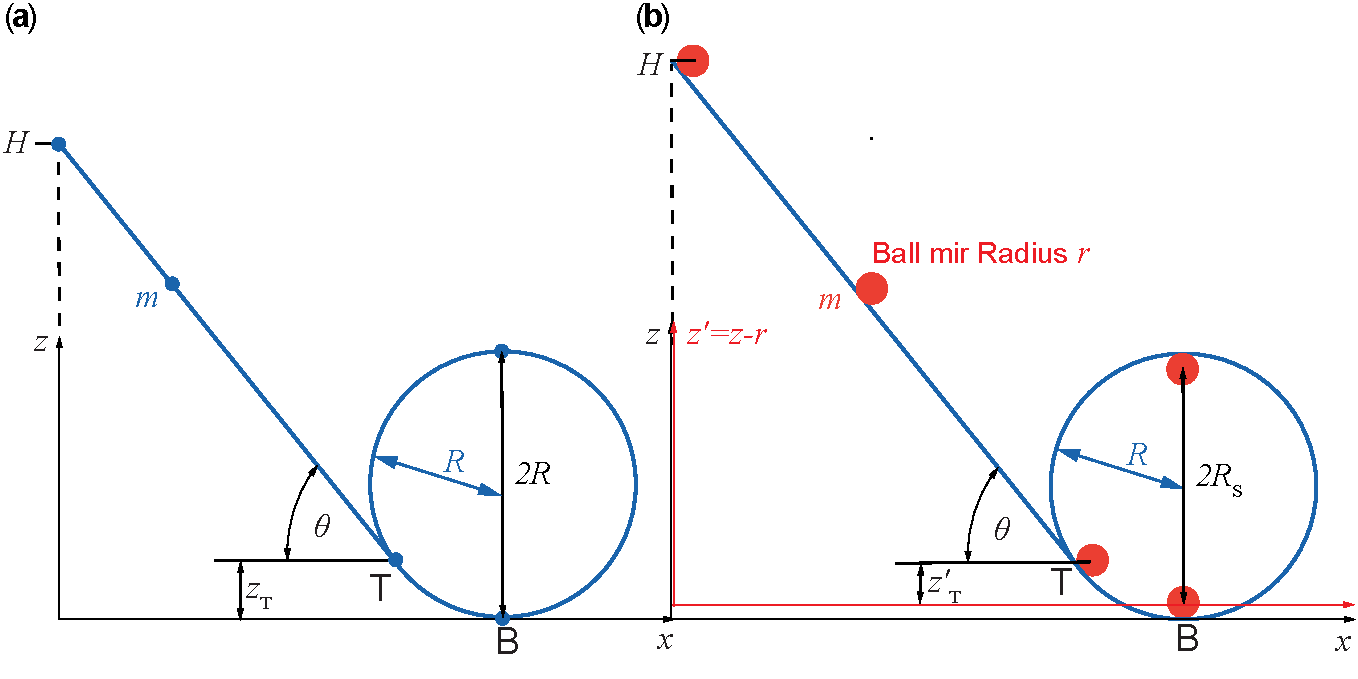
\includegraphics[width=\textwidth]{Loop2Loop.pdf}
\caption[Loop-the-Loop-Problem.]{\fa \textit{Loop-the-Loop}-Problem f�r einen Massepunkt. \fb \textit{Loop-the-Loop}-Problem f�r einen Ball mit Radius $r$.}\label{abb:bew_loop2loop}
\end{figure}

Wir wollen den Massepunkt (als Modell f�r einen einzelnen Wagen) auf der Bahn nach \figref{bew_loop2loop}a untersuchen und auch die Reibung ber�cksichtigen. Dabei wollen wir den auftretenden Ruck genauer untersuchen. Wir m�ssen drei Phasen der Bewegung unterscheiden:
\begin{enumerate}
    \item \textbf{Gleiten auf der geneigten Ebene} von $z=H$ bis zum Punkt T. Diesen Teil k�nnen wir analytisch berechnen und erhalten am Punkt T zum Zeitpunkt $t$ 
    \begin{align*}
        t_\text{T} = \sqrt{\frac{2\,\lk H-z\text{T}\rk}{g\,\lk\sin\theta - \mu_\text{G}\,\cos\theta\rk}}\,,
    \end{align*}
    die Geschwindigkeit
    \begin{align}
        v_\text{T} = \sqrt{2\,\lk H-z\text{T}\rk\,g\,\lk \sin\theta - \mu_\text{G}\,\cos\theta\rk } \label{eq:bew_Achterbahn60} \,,
    \end{align}
    worin $\mu_\text{G}$ der Gleitreibungskoeffizient ist. 
    \item \textbf{Eintritt in das Looping beim Punkt T }\\
    Diesen Abschnitt k�nnen wir nur numerisch berechnen. Am Eintrittspunkt f�hrt die pl�tzlich auftretende, durch die Schienen vermittelte Zwangskraft (Zentripetalkraft der Loop) zu einer in Richtung des Looping-Mittelpunktes auftretenden starken Beschleunigung (Ruck).\footnote{Den Ruck kann man auch als dritte Zeitableitung der Ortskoordinate verstehen, die sonst in der Physik wenig beachtet wird.} \\
    Die numerische Integration f�hren wir bis zum Punkt B, also $z=0$. Dort finden wir dann die Geschwindigkeit $v_\text{B}$.
    \item \textbf{Eigentliches Looping}\\
    Den Teil der Bewegung in der Loop vom Punkt B kann man interessanterweise analytisch geschlossen behandeln. \cite{Klobus2011}\\
    Wir beschreiben die Bewegung in der Koordinate $\varphi$ (siehe \figref{bew_loop2loop}a). \\
    Die Reibungskraft ist gegeben durch 
    \begin{align}
        F_\text{R} = \mu_\text{G}\,F_\text{N} = \mu_\text{G}\,\lk m\,g\,\cos\varphi + \frac{m}{R}\,v^2\lk\varphi\rk\rk\,.\label{eq:bew_Achterbahn61}
    \end{align}
    Dann gilt der Energieerhaltungssatz unter Ber�cksichtigung der durch die Reibungskraft $F_\text{R}$ \anf{geleisteten} Arbeit $W_\text{R}$
    \begin{align}
        \frac{m}{2}\,v_\text{B}{}^2 = \frac{m\,v^2\lk \varphi\rk}{2} + m\,g\,R\,\lk 1-\cos\varphi\rk + \underbrace{\int\limits_0^{s\lk\varphi\rk} F_\text{R}\lk s'\rk\,\D s'}_{W_\text{R}} \,.\label{eq:bew_Achterbahn62}
    \end{align}
    Mit $s\lk\varphi\rk = R\varphi$ f�r ein kreisf�rmiges Looping und damit $\D s = R\,\D\varphi$ k�nnen wir \eqref{eq:bew_Achterbahn62} integrieren:
    \begin{align*}
        \frac{m\,v^2}{2} =\,&\frac{m\,v_\text{B}{}^2}{2} - m\,g\,R + m\,g\,R\,\cos\varphi - \int\limits_0^{\varphi} F_\text{R}\lk\varphi'\rk\,R\,\D\varphi' \,,\\
        v^2 =\,&v_\text{B}{}^2 -2\,g\,R + 2\,g\,R\,\cos\varphi - 2\,\mu_\text{G}\,g\,\int\limits_0^{\varphi}R\,\cos\varphi'\,\D\varphi'- 2\,\mu_\text{G}\,\int\limits_0^{\varphi} v^2\,\D\varphi' \,,\\
    \end{align*}
    Wir f�hren noch zur Abk�rzung $u=v/\sqrt{g\,R}$, $u_\text{B} = v_\text{B}/\sqrt{g\,R}$ ein und erhalten:
    \begin{align}
        u^2 =\,&u_\text{B}{}^2 + 2\,\lk \cos\varphi - \mu_\text{G}\,\sin\varphi -1\rk - 2\,\mu_\text{G}\int\limits_0^\varphi u^2\lk \varphi'\rk\,\D\varphi'\,. \label{eq:bew_Achterbahn63}
    \end{align}
    Das ist eine sogenannte Volterra \gls{integralgleichung}\footnote{Vito Volterra 1860-1940 war ein italienischer Mathematiker, der vor allem auf den Gebieten der mathematischen Biologie und der Integralgleichungen forschte.}\indexp{Volterra, Vito}\index{Integralgleichung, Volterra-}. Die mathematische Behandlung dieser Integralgleichung geht �ber den Umfang dieses Buches hinaus, man findet aber die L�sung in guten Integraltafeln \cite{Gradshteyn1980, Bron2001} \bzw in \cite{Klobus2011}.\footnote{F�r den mathematische interessierten Leser sei erw�hnt, dass die Gl. \eqref{eq:bew_Achterbahn63} eine vereinfachte Form der Volterra Integralgleichung 2.~Art ist: $y\lk t\rk = H\lk t\rk + \int\limits_a^t K\lk t,s\rk\,y\lk s\rk\,\D s$ und daher relativ einfach zu l�sen ist. } Wir geben hier nur die L�sung an:
    \begin{align}
    \begin{split}
        u^2\lk\varphi\rk =\, &\e^{-2\,\mu_\text{G}\,\varphi}\,\lk u_\text{B}{}^2 + \frac{2\alpha}{\beta}\rk - \frac{2}{\beta}\,\lk \alpha\,\cos\varphi + 3\,\mu_\text{G}\,\sin\varphi\rk\\
        &\text{mit}~~~~ \alpha = 1+4\mu_\text{G}{}^2 ~~~~ \text{und} ~~~~ \beta = 2\mu_\text{G}{}^2 -1 \,. 
    \end{split} \label{eq:bew_Achterbahn64}
    \end{align}
    Damit k�nnen wir die Geschwindigkeit zu jedem Winkel $\varphi$ angeben, haben aber keine Zeitabh�ngigkeit $\varphi\lk t\rk$. Diese m�ssen wir uns numerisch wie gewohnt aus der Lagrange-Gleichung beschaffen, die hier einen Reibungsterm enth�lt. Wir empfehlen dem Leser das als relativ einfache �bung selbst durchzuf�hren.
\end{enumerate}
		%\mscr{} \mlbewref{loop2loop.m}
    Aus \eqref{eq:bew_Achterbahn64} lassen sich aber Aussagen gewinnen, welche Geschwindigkeit $v_\text{B}$ das Teilchen (der Wagen) beim Punkt $B$ haben muss, damit es (er) das Looping erfolgreich durchfahren kann. Wir k�nnen folgende 3 Bedingungen formulieren:
    \begin{align*}
        &\text{Bedingung 1:} ~~~~ u\lk\varphi\rk > 0 ~~~~ \text{f�r} ~~~~ \varphi <\frac{\pi}{2} \\
        &\text{Bedingung 2:} ~~~~ F_\text{N}\lk\varphi\rk > 0 ~~~~ \text{f�r} ~~~~ \frac{\pi}{2}\leq \varphi \leq \frac{3}{2}\,\pi \\
        &\text{Bedingung 3:} ~~~~ u\lk\varphi\rk > 0 ~~~~ \text{f�r} ~~~~ \varphi > \frac{3}{2}\,\pi
    \end{align*}
    Wird Bedingung 1 verletzt, bleibt der Wagen im 1. Quadranten des Loopings stecken, analog bei Verletzung von Bedingung 3 im 4. Quadranten. Wird Bedingung 2 verletzt, dann \anf{f�llt} der Wagen von der oberen Kreish�lfte nach unten, und das will ja nun wirklich niemand. \\
    Man kann relativ einfach aus der L�sung \eqref{eq:bew_Achterbahn64} der Integralgleichung ein Stabilit�tsdiagramm berechnen, in dem man auf der $x$-Achse die Anfangsgeschwindigkeit $v_\text{B}$ (\bzw daraus abgeleitet die Anfangsh�he $H$) und auf der $y$-Achse den Gleitreibungskoeffizienten $\mu_\text{G}$ auftr�gt und die Stabilit�tsgrenzen f�r das jeweilige Parameterpaar bestimmt. Dies sei dem Leser in \probref{bew_loop2loop} empfohlen. Ebenso wollen wir das Problem des rollenden Balls von \figref{bew_loop2loop}b, bei dem wir die vom Ball aufgenommene Rotationsenergie ber�cksichtigen m�ssen, in \probref{bew_loop2loop} untersuchen.
		
\subparagraph{\textbf{Bewegung auf Spiralen}}

		Wir wollen noch eine Bemerkung zum Ruck machen. Das gerade beschriebene Problem des Looping Eintritts am Punkt T tritt immer bei Einfahrt und Ausfahrt von Kurven in Geraden auf, so auch \zb in horizontalen Ebene im Stra�enbau. Die Vermeidung \bzw Minimierung des Rucks wurde durch Benutzung von spezifischen, nicht-kreisf�rmigen Kurvenformen gel�st. Besonders ausgezeichnet hat sich dabei die Klothoide\index{Klothoide}, welche auch als Cornu-Spirale\index{Cornu-Spirale}\indexp{Cornu, Marie Alfred}\footnote{Marie Alfred Cornu (1841-1902) war ein franz�sicher Physiker der sich besonders durch hoch genaue Messtechniken zur Messung der Gravitationskonstante $G$ und der Lichtgeschwindigkeit $c$ auszeichnete.} bekannt ist. \\
    Bei dieser Kurve ist der lokale Kr�mmungsradius $\varrho$ invers zur Bogenl�nge $s$:
    \begin{align*}
        \varrho = \frac{p^2}{s}\,,
    \end{align*}
    worin $p$ der sogenannte Klothoidenparameter ist. Die Klothoide kann durch folgende Integraldarstellung \figref{bew_Klothoide} beschrieben werden:
    \begin{subequations}
        \begin{align}
            x\lk t\rk &= p\,\sqrt{\pi}\int\limits_0^t\cos\lk \frac{\pi}{2}\,t'{}^2\rk\,\D t' ~~~~ \text{mit} ~~~~ t = \frac{s}{\sqrt{p\,\pi}}\;,  \label{eq:bew_Achterbahn65a}\\
            z\lk t\rk &= p\,\sqrt{\pi}\int\limits_0^t\sin\lk \frac{\pi}{2}\,t'{}^2\rk\,\D t' ~~~~ \text{mit} ~~~~ t = \frac{s}{\sqrt{p\,\pi}}\;.\label{eq:bew_Achterbahn65b}
        \end{align}
    \end{subequations}

\begin{figure}
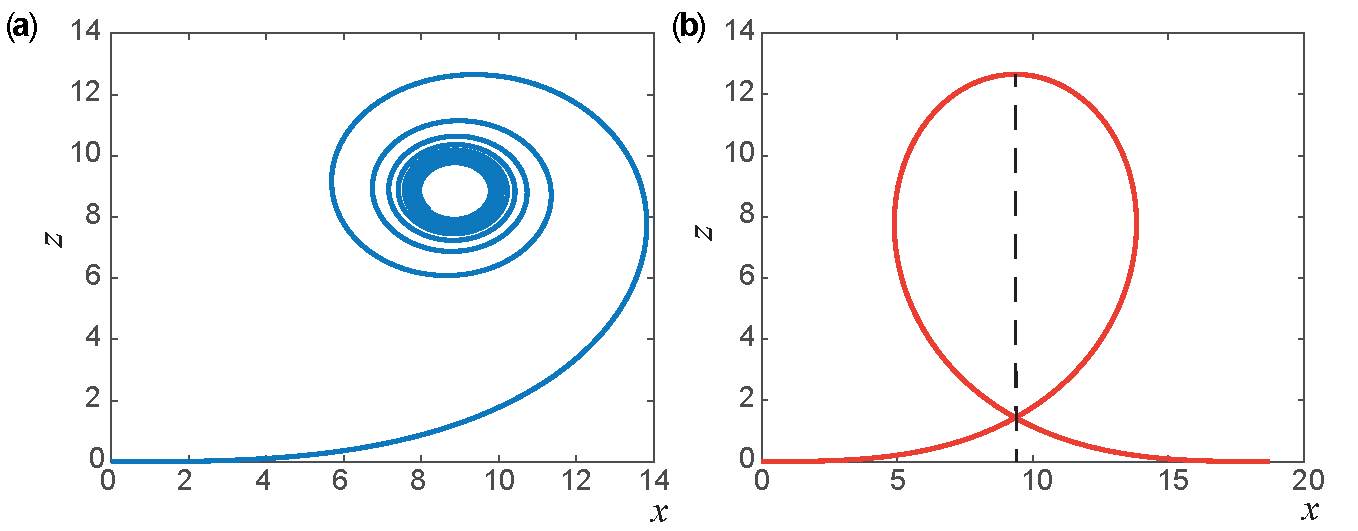
\includegraphics[width=\textwidth]{Klothoide.pdf}
\caption[Klothoide und Looping in Form zweier Klothoiden�ste.]{\fa Klothoide und \fb Looping in Form zweier Klothoiden�ste. Berechnung im  \mscr{} \mlbewref{Klothoide.m}.}\label{abb:bew_Klothoide}
\end{figure}

    F�r ein Stra�en- \bzw Achterbahndesign nimmt man nat�rlich nur den Ast bis zum ersten positiven Maximum und spiegelt dann die Kurve. Bei den Stellen  $s=0 $ und $s=2\,s_\text{max}$ wird dann beim Einfahren aus einer Geraden kein Ruck auftreten, da dort der Kr�mmungsradius $\infty$ ist (siehe auch \cite{Heintz2009}).


\subparagraph{\textbf{Zug im kreisf�rmigen Looping}}

Wir wollen nun den Zug der L�nge $l_\text{Z}$ in einen Kreis-Looping mit dem Radius $R$ untersuchen, was die Situation etwas komplexer macht. Es gibt neben der Zentrifugalkraft eine zus�tzliche Spannungskraft zwischen den einzelnen Wagen des Zuges, die tangential zu der Bahn wirkt und daf�r sorgt, dass alle Wagen im Zug die gleiche Geschwindigkeit und tangentiale Beschleunigung haben. Der Zug habe eine homogene Massenverteilung $\mu = M/l_\text{Z}$. Wir w�hlen das KOS entsprechend \figref{bew_ZugKreisring}. In der Abbildung haben wir zwei Situationen dargestellt, die im Folgenden auch gesondert untersucht werden m�ssen. Sobald der Zug im Loop eingefahren ist, kann das System mit der generalisierten Koordinate $\varphi_\text{F}$ beschrieben werden.\\
Wir wollen berechnen, mit welcher Mindestgeschwindigkeit der Zug in die Kreisbahn-Loop einfahren muss, damit er st�ndig im Kontakt mit der Bahn bleibt. Dazu gen�gt es, die Energieerhaltung und die Spannungskr�fte innerhalb des als Seils/Kette beschriebenen Zuges zu ber�cksichtigen. Ein Massenelement innerhalb des Zuges (in der Loop) ist gegeben durch:
\begin{align}
    \D m = \mu\,R\,\D\varphi = \frac{M}{l_\text{Z}}\,R\,\D\varphi\,. \label{eq:bew_Achterbahn41}
\end{align}
Aus der Energieerhaltung folgt:
\begin{align}
    \frac{M}{2}\,v_0{}^2 = \underbrace{\frac{M}{2}\,v_\text{F}{}^2}_{T\lk \varphi_\text{F}\rk} + \underbrace{\int\limits_{\varphi_\text{E}}^{\varphi_\text{F}} \mu\,g\,R^2\,\lk 1-\cos\varphi\rk\,\D\varphi}_{U\lk \varphi_\text{F}\rk}\,.\label{eq:bew_Achterbahn42}
\end{align}

\begin{figure}
\begin{minipage}{\textwidth}
\leftfigure{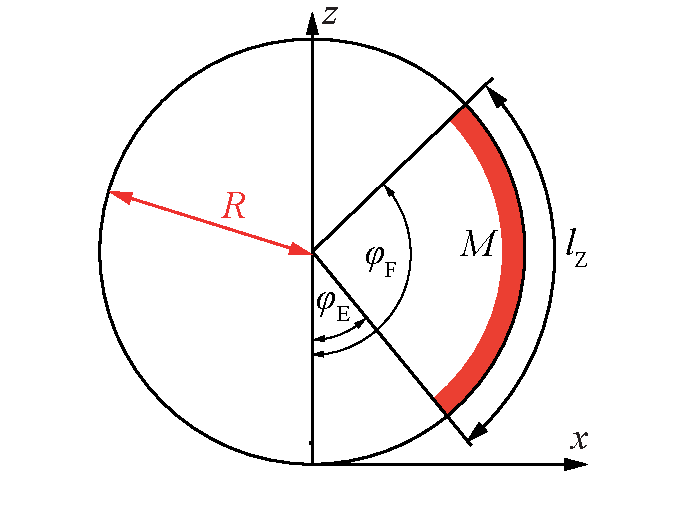
\includegraphics[width=0.5\textwidth]{AchterbahnKreisring.pdf}}%
\hspace{\fill} 
\rightfigure{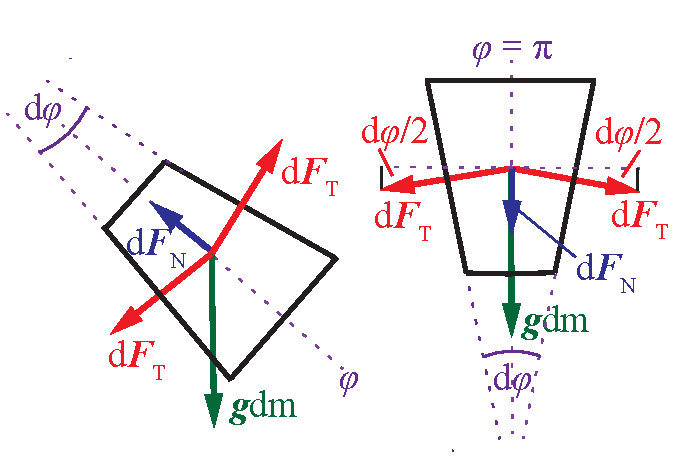
\includegraphics[width=0.5\textwidth]{AchterbahnTangentialK.pdf}}%
\leftcaption[Zug in einem Kreisring als Beispiel f�r ein Looping.]{Zug in einem Kreisring als Beispiel f�r ein Looping.} \label{abb:bew_ZugKreisring}
\rightcaption[Tangentialkr�fte in einem Seil im Kreisring.]{Tangentialkr�fte in einem Seil im Kreisring.} \label{abb:bew_Spannungskraefte}
\end{minipage}
\end{figure}

Hierin sind $v_0$ die Anfangsgeschwindigkeit des Zuges, $v_\text{F}$ die momentane Geschwindigkeit des Zuges wenn der Zuganfang sich bei $\varphi_\text{F}$ befindet ($v_\text{F} = R\,\dot{\varphi}_\text{F}$). Der Potentialterm $U\lk \varphi_\text{F}\rk$ ergibt sich mit der Position des Zugendes $\varphi_\text{E}$ aus der Integration zu:
\begin{subequations}
\begin{align}
  \text{(a): }&~~l_\text{Z}> R\,\varphi_\text{F}\;,~~ \varphi_\text{E}=0 \;, \nonumber \\
		U\lk \varphi_\text{F}\rk &=  \mu\,g\,R^2\,\lek \varphi_\text{F} - \sin\varphi_\text{F}\rek ~~ \,, \label{eq:bew_Achterbahn43a} \\
  %\text{(b):}~~  U\lk \varphi_\text{F}\rk &=  \mu\,g\,R^2\,\lek \frac{l_\text{Z}}{R} - \lk \sin\varphi_\text{F} - \sin\lk \varphi_\text{F} - \frac{l_\text{Z}}{R}\rk \rek ~~ &\text{f�r} ~~ l_\text{Z} < R\,\varphi_\text{F} \equiv \varphi_\text{E} = \varphi_\text{F} - \frac{l_\text{Z}}{R} > 0\,, \varphi_\text{F}\leq 2\pi \, \label{eq:bew_Achterbahn43b}
  % TODO: in der oben auskommentierten Zeile fehlte ein \rk, ich habe unten das \lk entfernt
  \text{(b): }&~~l_\text{Z} < R\,\varphi_\text{F} \,,~~ \varphi_\text{E} = \varphi_\text{F} - \frac{l_\text{Z}}{R} > 0\,,~~ \varphi_\text{F}\leq 2\pi \, \nonumber \\
		U\lk \varphi_\text{F}\rk &=  \mu\,g\,R^2\, \lek \frac{l_\text{Z}}{R} - \sin\varphi_\text{F} + \sin\lk \varphi_\text{F} - \frac{l_\text{Z}}{R}\rk \rek ~\,.\label{eq:bew_Achterbahn43b}
\end{align}
\end{subequations}
Aus \eqref{eq:bew_Achterbahn42} folgt 
\begin{subequations}
\begin{align}
    \text{(a):} ~~ v_\text{F}{}^2 &= v_0{}^2 - \frac{2\,\mu\,g\,R^2}{M}\,\lk \varphi_\text{F} - \sin\varphi_\text{F}\rk\,,\label{eq:bew_Achterbahn44a} \\
    %\text{f�r den Fall (b):} ~~ v_\text{F}{}^2 = v_0{}^2 - \frac{2\,\mu\,g\,R^2}{M}\,\lk \frac{l_\text{Z}}{R} - \lk \sin\varphi_\text{F} - \sin\lk \varphi_\text{F} - \frac{l_\text{Z}}{R}\rk \rk\,,\label{eq:bew_Achterbahn44b}
    % TODO: in der oben auskommentierten Zeile fehlte ein \rk, ich habe unten das \lk entfernt
    \text{(b):} ~~ v_\text{F}{}^2 &= v_0{}^2 - \frac{2\,\mu\,g\,R^2}{M}\,\lk \frac{l_\text{Z}}{R} - \sin\varphi_\text{F} + \sin\lk \varphi_\text{F} - \frac{l_\text{Z}}{R}\rk \rk\,,\label{eq:bew_Achterbahn44b}
\end{align}
\end{subequations}
woraus man sehr einfach die Differentialgleichung f�r den Zug ableiten kann, in dem man \eqref{eq:bew_Achterbahn44a} \bzw \eqref{eq:bew_Achterbahn44b} nach der Zeit differenziert, woraus man wiederum die zeitliche Entwicklung f�r $\varphi$ numerisch in \matlab{} berechnen kann. \\

\begin{nebenrechnung}

\begin{subequations}
\begin{align}
    \text{(a):}&~~ v_\text{F}{}^2 = R^2\,\dot{\varphi}_\text{F}{}^2 = v_0{}^2 - \frac{2\,\mu\,g\,R^2}{M}\,\lk \varphi_\text{F} - \sin\varphi_\text{F}\rk \nonumber \\
    %2\,R^2\,\dot{\varphi}_\text{F}\,\ddot{\varphi}_\text{F} &= -\frac{2\,\mu\,g\,R^2}{M}\,\lk\dot{\varphi}_\text{F} - \cos\varphi_\text{F}\,\dot{\varphi}_\text{F}\rk \nonumber \\
    \rightarrow ~~~~ \ddot{\varphi}_\text{F} &=  \frac{\mu\,g}{M}\,\lk \cos\varphi_\text{F} - 1\rk  \label{eq:bew_Achterbahn45a} \\
		\nonumber \\
    \text{(b):} &~~ v_\text{F}{}^2 = R^2\,\dot{\varphi}_\text{F}{}^2 = v_0{}^2 - \frac{2\,\mu\,g\,R^2}{M}\,\lek \frac{l_\text{Z}}{R} -\,\lk \sin\varphi_\text{F} - \sin\lk \varphi_\text{F} - \frac{l_\text{Z}}{R}\rk\rk\rek \nonumber \\
    \rightarrow ~~~~ \ddot{\varphi}_\text{F} &= \frac{\mu\,g}{M}\,\lek \cos\varphi_\text{F} - \cos\lk \varphi_\text{F}-\frac{l_\text{Z}}{R}\rk\rek \label{eq:bew_Achterbahn45b}
\end{align}
\end{subequations}

\end{nebenrechnung}

Wir ben�tigen jetzt noch wie eingangs erw�hnt die internen Spannungskr�fte im Zug (Seil), also die Kr�fte die zwischen den einzelnen Wagen von den Kupplungen vermittelt werden. Wir k�nnten uns diese aus den Lagrange-Multiplikatoren beschaffen (siehe \probref{bew_achterbahn}). Es gibt aber einen etwas einfacheren Weg, in dem wir die an jedem Massenelement am Ort $\varphi$ wirkenden differentiellen Tangentialkr�fte integrieren. Die differentielle Tangentialkraft ist nach \figref{bew_Spannungskraefte} gegeben durch:
\begin{align}
     \D F_\text{T} &= \D m\,g\,\sin\varphi = g\,\mu\,R\,\sin\varphi\,\D \varphi \nonumber \\
     \rightarrow ~~~~ F_\text{T}\lk \varphi\rk &= \int\limits_{\varphi_\text{E}}^{\varphi}g\,\mu\,R\,\sin\varphi\,\D\varphi = -g\,\mu\,R\,\cos\varphi\,\Big|_{\varphi_\text{E}}^{\varphi} ~~~(\varphi_\text{E} \geq 0) \,.\label{eq:bew_Achterbahn47}
\end{align}
$F_\text{T}\lk \varphi\rk$ ist die am \anf{Ort} $\varphi$ wirkende Tagentialkraft, die wir in der differentiellen N�herung als interne Spannungskraft verstehen k�nnen. Die kritische Situation f�r den Zug in der Loop besteht wenn der Mittelteil des Zuges am oberen Punkt der Loop angekommen ist, \dh
\begin{align*}
    \varphi_\text{F} &= \pi + \frac{l_\text{Z}}{2R}\,, & \varphi_\text{E} = \pi - \frac{l_\text{Z}}{2R}\,, ~~~~ l_\text{Z} \leq 2\pi R  \,.
\end{align*}
F�r den Betrag der Tangentialkraft gilt:
\begin{align}
    F_\text{T}\lk\varphi=\pi\rk & = -g\,\mu\,R\,\cos\varphi\,\Big|_{\pi-\frac{l_\text{Z}}{2R}}^\pi = -g\,\mu\,R\,\lek -1-\cos\lk\pi-\frac{l_\text{Z}}{2R}\rk\rek \nonumber \\
		& = g\,\mu\,R\,\lek 1-\cos\lk\frac{l_\text{Z}}{2R}\rk\rek \; . \label{eq:bew_Achterbahn48}
\end{align}
Am oberen Punkt des Kreises muss die differentielle Kr�ftebilanz wie folgt aussehen:
\begin{align}
    \D \vec{F}_\text{G} + \D \vec{F}_\text{N}\lk \pi \rk  = \D \vec{F}_\text{G} + \D \vec{F}_\text{T}\lk \pi \rk   = \D \vec{F}_\text{Z}\,, \label{eq:bew_Achterbahn48a}
\end{align}
worin $\D \vec{F}_\text{Z}$ die auf das Massenelement $\D m$ wirkende Zentrifugalkraft mit $R\dot{\varphi}_\text{F}^2\,\D m = R\dot{\varphi}\,\lk \pi + \frac{l_\text{Z}}{2R}\rk^2 \,\D m$ ist. Wir benutzen \figref{bew_Spannungskraefte} und setzen \eqref{eq:bew_Achterbahn48} sowie \eqref{eq:bew_Achterbahn44a} in \eqref{eq:bew_Achterbahn48a} ein und erhalten f�r die $z$-Komponente der Kr�ftebilanz \eqref{eq:bew_Achterbahn48a}:
\begin{align}
    g\,\D m + 2\,g\,\mu\,R\,\lk 1 - \cos\lk \frac{l_\text{Z}}{2R}\rk\rk\,\sin\lk \frac{\D \varphi}{2}\rk &= R\,\dot{\varphi}_\text{F}{}^2\,\D m \nonumber \\
    \mu\,g\,R\,\D\varphi + 2\,g\,\mu\,R\,\lk 1-\cos\lk \frac{l_\text{Z}}{2R}\rk\rk\, \frac{\D \varphi}{2} &\approx \mu\,R^2\,\dot{\varphi}_\text{F}{}^2\,\D\varphi \nonumber \\
    \rightarrow~~~ \frac{g}{R}\,\lk 2-\cos\lk \frac{l_\text{Z}}{2R}\rk\rk & = \dot{\varphi}_\text{F}{}^2 \,. \label{eq:bew_Achterbahn49}
\end{align}
Mit der Beziehung \eqref{eq:bew_Achterbahn44b}, die aus der Energieerhaltung abgeleitet wurde, erhalten wir mit $v_\text{F} = R \dot{\varphi}_\text{F}$,  $\varphi_\text{F} = \pi + l_\text{Z}/2R \, \varphi_\text{E} = \pi - l_\text{Z}/2R $:
\begin{align}
    %v_0{}^2 & = g\,R\,\lk 2-\cos\lk\frac{l_\text{Z}}{2R}\rk\rk + \frac{2\,\mu\,g\,R^2}{M}\,\lek \varphi_\text{F} - \sin\varphi_\text{F} - \lk \varphi_\text{E} - \sin\varphi_\text{E} \rk \rek  \nonumber \\
    v_0{}^2 & =  g\,R\,\lk 2-\cos\lk\frac{l_\text{Z}}{2R}\rk\rk + \frac{2\,\mu\,g\,R^2}{M}\,\lek \frac{l_\text{Z}}{R} + 2\,\sin\lk \frac{l_\text{Z}}{2R}\rk\rek \,. \label{eq:bew_Achterbahn50}
\end{align}
Man kann die Spezialf�lle $l_\text{Z}=0$ (einzelner Wagen als Massepunkt), $l_\text{Z}=2\,\pi\,R$ (Kreisring vollst�ndig gef�llt durch Zug) und $l_\text{Z}=\pi\,R$ (Kreisring zur H�lfte gef�llt durch Zug) leicht berechnen.
\begin{align*}
l_\text{Z} \to 0 ~~ &\text{mit} ~~ \mu{}\,l_\text{Z}/M \to 1: \\
    v_0{}^2(l_\text{Z} \to 0) &= g\,R\, + \lim_{l_\text{Z} \to 0,\mu{}l_\text{Z}/M \to 1}  \lek \frac{\mu}{M} 2 \,g\,R^2 \lk \frac{l_\text{Z}}{R} +2\,\sin\frac{l_\text{Z}}{2R} \rk \rek \\
										 &= \,g\,R \,+ 2 \,g\,R\,(1+1) = 5 \,g\,R \,, \\ \\
l_\text{Z} = 2\pi\,R~~ &\text{mit} ~~ \mu{}\,l_\text{Z}/M = 1: \\
    v_0{}^2(l_\text{Z}=2\pi R) &= g\,R\,\lk 2+1\rk + 2\,\frac{\mu}{M}\,g\,R^2 \lek 2\pi + 2\sin\lk \frac{2\,\pi\,R}{2R}\rk \rek \\
		                 &= 3\,g\,R \,+ 2\,\frac{\mu}{M}\,g\,R^2(2\pi + 0) = 5\,g\,R \,, \\ \\
l_\text{Z} = \pi\,R~~ &\text{mit} ~~ \mu{}\,l_\text{Z}/M = 1: \\ 
    v_0{}^2(l_\text{Z}=\pi R) &= g\,R\,\lk 2 + 0\rk +2\,\frac{\mu}{M}\,g\,R^2 \lek \pi + 2\sin\lk \frac{\pi\,R}{2R}\rk \rek \\
		                 &= 2\,g\,R \,+ 2\,\frac{\mu}{M}\,g\,R^2(\pi + 2) = 2\,g\,R \,\lk 1 + 1 + \frac{2}{\pi} \rk = 4\,g\,R \,\lk 1+ \frac{1}{\pi} \rk \,.
\end{align*}
Das Ergebnis ist insofern interessant, als dass ein Seil der L�nge $2 \pi R$ und gleicher Masse $M$ die gleiche Anfangsgeschwindigkeit braucht wie ein einzelne Massepunkt der Masse $M$ , um die Loop sicher zu durchlaufen (Reibung vernachl�ssigt). Man kann sich das aber auch klar machen, in dem man eine Energiebetrachtung aus dem Inertialsystem heraus macht und ber�cksichtigt, dass dort die Rotationsenergie von Massepunkt und Ring (= Seil) unter den angenommenen Bedingungen gleich gro� sind. 

In \probref{bew_achterbahn} behandeln wir die Dynamik von Massepunkten und Z�gen auf gekr�mmten Kurven (wie sie bei der Achterbahn auftreten) etwas allgemeiner.
%wobei wir ebenfalls das Modell der Kette unter dem Einfluss verschiedener Kr�fte und Zwangsbedingungen betrachten wollen. 
In \probref{bew_achterbahn_diskret} untersuchen wir ein diskretes Modell eines Zuges auf einer beliebigen Kurve, welches wir nach der das in \probref{bew_achterbahn_vergleich} mit dem hier ausgearbeiteten Modell eines starren Zuges der L�nge $l_\text{Z}$ vergleichen.
Mit den in der Mechanik der Kontinua (Kapitel 2) entwickelten Methoden werden wir dann in \probref{kontmech_AchterbahnKont} bis \probref{kontmech_AchterbahnBeschleunigungen} ein Modell eines erweitertes Modell eines "`teilelastischen"' Zuges behandeln k�nnen.

\subsubsection{Dynamik einer fallenden Kette und Bungee-Jumping} \label{kap:bew_chains}

\subparagraph{\textbf{Fallende Kette}} \index{Kette!fallende} 

Ein interessantes Problem ist das der fallenden Kette (siehe auch \cite{Wong2006,Calkin1989}).
Dieses Problem beinhaltet die Dynamik einer ver�nderlichen Masse, wie wir dies in �hnlicher Form beim Raketenstart im Kapitel Astrodynamik betrachten werden.
Interessanterweise wurde das Problem in vielen Lehrb�chern der Physik bis in die 1980er Jahre hinein \zt falsch beschrieben, obwohl bereits Lagrange%
\indexp{Lagrange, Joseph-Louis} alle Methoden zu dessen Behandlung aufgezeigt hatte. 
\begin{figure}
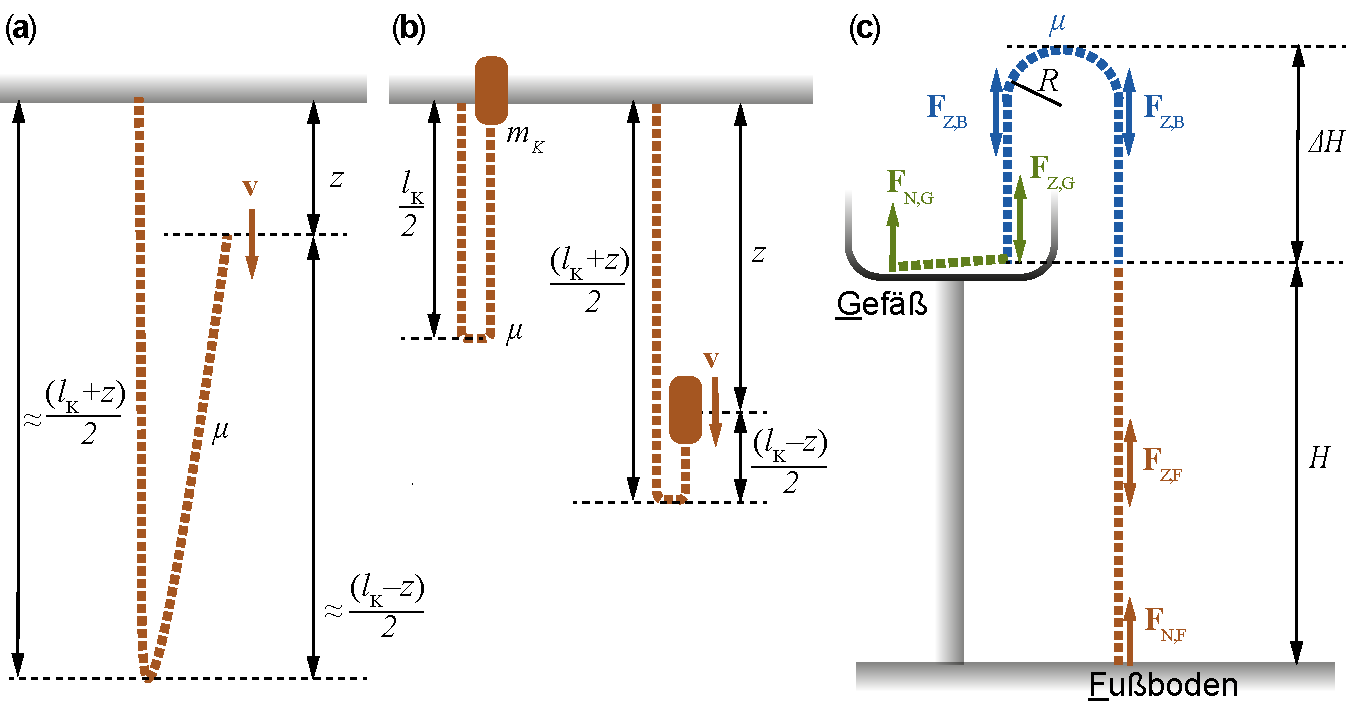
\includegraphics[width=0.95\textwidth]{FallingChain01.pdf}
\caption[Modell der fallenden Kette und Beispiele.]{Modell der fallenden Kette und Beispiele. \fa Grundmodell ($\mu$ Masse der Kette pro L�ngeneinheit. \fb Modell f�r Bungee-Jumping ($m_\text{K}$ Masse des K�rpers, $v$ Geschwindigkeit in Fallh�he $z$. \fc Kettenfont�ne und wirkende Kr�fte. Zur besseren Unterscheidung der Einheiten der Kette sind diese farblich unterschiedlich gekennzeichnet, es handelt sich aber um eine homogene Kette mit der Massendichte $\mu$.}\label{abb:bew_FallingChain01}
\end{figure}
Einer der interessantesten Effekte der fallenden Kette ist die Tatsache, dass das lose Ende der Kette schneller fallen kann als ein K�rper im freien Fall, obwohl als �u�ere Kraft nur die Schwerkraft wirkt. Wir wollen das erkl�ren und schreiben dazu mit \figref{bew_FallingChain01} die Lagrange-Funktion auf:
        \begin{align}
            \mathcal{L}\lk z,\dot{z}\rk = T(z) - U(z) = \frac{\mu}{4}\,\lk l_\text{K}-z\rk\,\dot{z}^2 + M\,g\,\lk \frac{l_\text{K}^2+2z\,l_\text{K}-z^2}{4 l_\text{K}}\rk\,. \label{eq:bew_FallingChain01}
        \end{align}
Wir halten ferner fest, das folgende Beziehungen gelten:
        \begin{align*}
            m_\text{L} &= \mu\,b_\text{L}\,, & m_\text{R}&= \mu\,b_\text{R}\,, \\
            b_\text{L} &= \frac{1}{2}\,\lk l_\text{K}+z\rk\,, & b_\text{R} &= \frac{1}{2}\,\lk l_\text{K}-z\rk \,,\\
            z_\text{L} &= \frac{1}{4}\,\lk l_\text{K}+z\rk\,, & z_\text{R} &= \frac{1}{4}\,\lk l_\text{K}+3z\rk\,,
        \end{align*}
worin $\mu$ die homogene Massendichte $\mu = M/l_\text{K}$, $b_\text{i}$ die L�nge, $z_\text{i}$ der Schwerpunkt, und $m_\text{i}$ die Masse des linken ($i=L$) bzw. rechten ($i=R$) Arms der Kette sind. Offensichtlich ist $\d \mathcal{L}/\d t = 0 $. Die Hamilton-Funktion (siehe Definition \eqref{eq:bew_Hamilton_Fkt})
        \begin{align}
            \mathcal{H} = \underbrace{\frac{\d\mathcal{L}}{\d \dot{z}}\cdot\dot{z}}_{p_\text{R}\,v} - \mathcal{L}\lk z,\dot{z}\rk = \frac{{p_\text{R}}^2}{2m_\text{R}} - M\,g\,\lk \frac{l_\text{K}^2+2z\,l_\text{K}-z^2}{4 l_\text{K}}\rk = E \label{eq:bew_FallingChain03}
        \end{align}
ist daher nach \kapitel{bew_Lagrange_II} gleich der Energie $E$, da das System konservativ ist. Mit der aus der Lagrange-Funktion berechneten Lagrange-Gleichung und unter Verwendung von $\dot{z} = v$ und $\ddot{z} = \dot{v}$ schreiben wir:
%\footnote{Man kann auch einfacher dies aus der Hamilton-Funktion erhalten, indem man $\frac{\d p}{\d t} = -\frac{\d \mathcal{H} t}{\d t}$ bildet.}
        \begin{align}
            \dot{p}_\text{R} = m_\text{R}\,\dot{v} + \dot{m}_\text{R}\,v = m_\text{R}\,g - \frac{1}{4}\,\mu\,v^2 \,.\label{eq:bew_FallingChain04}
        \end{align}
Man erkennt an \eqref{eq:bew_FallingChain04} sehr sch�n die zeitlich ver�nderliche Masse und einen daraus folgenden Zusatzterm $-\frac{1}{4}\,\mu\,v^2$, der der Schwerkraft entgegen wirkt und eine innere Spannung der Kette darstellt. Dieser Term ist f�r die zus�tzliche Beschleunigung des rechten Arms der Kette verantwortlich, der zu gr��eren Fallgeschwindigkeiten f�hrt, als sie im freien Fall auftreten. Gl. \eqref{eq:bew_FallingChain04} ist eine nichtlineare Differentialgleichung.\\
Aus der Energieerhaltung $U_0 = -M\,g\,l_\text{K}/4 = T(z) + U(z)$ findet man leicht
        \begin{align}
        \begin{split}
            v^2\lk z\rk &= 2g\,x\,\frac{\lk 1-\frac{1}{2}\,\frac{z}{l_\text{K}}\rk}{\lk 1-\frac{z}{l_\text{K}}\rk} \\
            &\approx 2g\,z\,\lek 1+\frac{1}{2}\,\lk \frac{z}{l_\text{K}} + \lk \frac{z}{l_\text{K}}\rk^2 +\ldots \rk\rek = {v_\text{F}}^2\,\lek 1+\frac{1}{2}\,\lk \frac{z}{l_\text{K}} + \lk \frac{z}{l_\text{K}}\rk^2 +\ldots \rk\rek\,, \label{eq:bew_FallingChain05}
        \end{split}
        \end{align}
worin $v_\text{F} = \sqrt{2g\,z}$ die Geschwindigkeit des freien Falls ist. \\
Die DGL \eqref{eq:bew_FallingChain04} k�nnen wir numerisch l�sen. %Der Ansatz
	%\[\dot{v} = \frac{1}{2}\,\frac{\D v^2}{\D z} = v\,\frac{\D v}{\D t}\,\frac{\D t}{\D z}
	%\]
%auf eine inhomogene Differentialgleichung f�r $v^2$. 
In \figref{bew_FallingChain02} zeigen wir die numerische L�sung $v\lk t\rk$, $z\lk t\rk$ im Vergleich zum freien Fall (\mlbewref{FallingChain01.m})  Deutlich ist die Beschleunigung gr��er als $g$ zu erkennen.

\begin{figure}
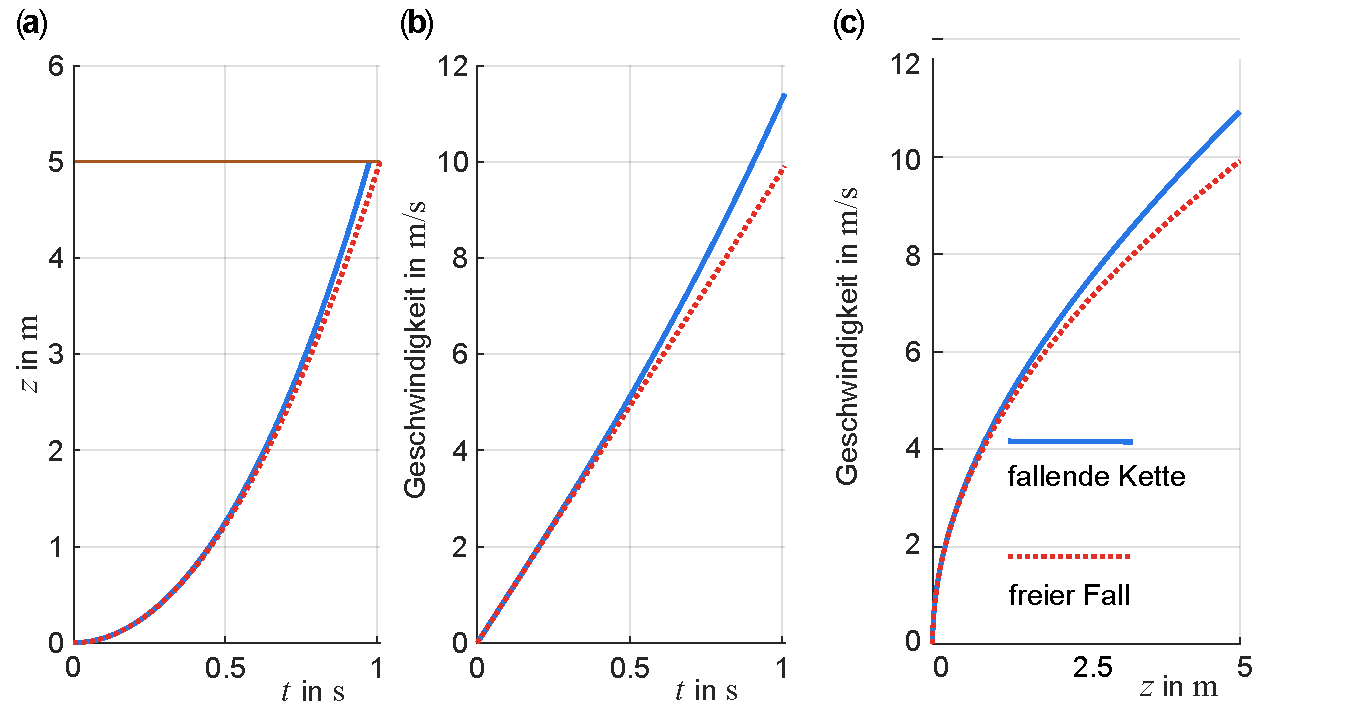
\includegraphics[width=\textwidth]{FallingChain02.pdf}
\caption[Dynamik der fallenden Kette im Vergleich zum freien Fall.]{Dynamik der fallenden Kette im Vergleich zum freien Fall. Man sieht, dass am Ende der Fallperiode die Geschwindigkeit der fallenden Kette gr��er ist als die des freien Falls. Die Fallzeit der Kette in unserem Modell ist unabh�ngig von der Massendichte $\mu$. }\label{abb:bew_FallingChain02}
\end{figure}

Wir wollen jetzt noch eine Erkl�rung daf�r geben, dass die Spannung $F_\text{T} = -\mu\,v^2/4$ in \eqref{eq:bew_FallingChain04} der Schwerkraft entgegen wirkt und nicht, wie man vielleicht erwarten k�nnte, in Richtung von $g$. Schreibt man \eqref{eq:bew_FallingChain04} in Newtonscher Form, also 
        \begin{align*}
            m_\text{R}\,\dot{v} = m_\text{R}\,g - \underbrace{\lk \dot{m}_\text{R}\,v + \frac{1}{4}\,\mu\,v^2 \rk}_{= F_\text{T,eff}}\,,
        \end{align*}
dann ergibt der gesamte Zusatzterm $F_\text{T,eff}$ wegen $\dot{m}_\text{R}<0$ eine zus�tzliche Kraft in Richtung der Schwerkraft. Wir wollen uns jetzt noch zwei konkrete Anwendungen dieser bisher eher theoretischen �berlegungen anschauen. 

\subparagraph {\textbf{Bungee-Jumping}} \index{Bungee-Jumping}

Eine Art "`Kettenproblem"' liegt auch beim Bungee-Jumping (\figref{bew_FallingChain01}b) vor. Die Lagrange-Funktion k�nnen wir wieder einfach aufschreiben, der einzige Unterschied zu \eqref{eq:bew_FallingChain01} ist das Auftreten der Zusatzmasse $m_\text{K}$ des Bungee-Springers.

Die Lagrange Funktion lautet dann:
\begin{align}
\begin{split}
    \mathcal{L} = &T-U \\
    = &\underbrace{\lek \frac{1}{2}\,m\,\frac{l_\text{K}-z}{2 l_\text{K}}\,\dot{z}^2 + \frac{1}{2}\,m_\text{K}\,\dot{z}^2 \rek }_{T} \\
		  &- \underbrace{\lek -m\,\frac{l_\text{K}-z}{2 l_\text{K}}\,g\,\lk z + \frac{l_\text{K}-z}{4}\rk \rek }_{U_1} 
			 - \underbrace{\lek - m\,\frac{l_\text{K}+z}{2 l_\text{K}}\,g\,\frac{l_\text{K}+z}{4} \rek}_{U_2} - \underbrace{m_\text{K}\,g\,z}_{U_3}\,.
\end{split} \label{eq:bew_Bungee01}
\end{align}
Hierin sind $U_1$ die potentielle Energien des bereits gefallenen Bandes, $U_2$ die des noch h�ngenden Bandes und $U_3$ die potentielle Energie des Springers. Die Geschwindigkeit des Springers ergibt sich direkt aus der Energieerhaltung, dabei ist die Anfangsenergie (das Nullpotential liege bei $z=0$) gegeben durch:
\begin{align*}
    E_0 = -m\,g\,\frac{l_\text{K}}{4}\,.
\end{align*}
Daraus folgt mit $E_0 = T + U_1 +U_2+U_3 $ aus \eqref{eq:bew_Bungee01}: 
\begin{align}
    v^2\lk z\rk = \dot{z}^2 = g\,z\,\frac{4m_\text{K}\,l_\text{K} + 2m\,l_\text{K} -m\,z}{m\,l_\text{K}-m\,z + 2m_\text{K}\,l_\text{K}} \label{eq:bew_Bungee02}
\end{align}
und speziell f�r $z=l_\text{K}$ (am Ende des Sprunges) zu
\begin{align}
    v_\text{f}{}^2 = v^2\lk l_\text{K}\rk = 2g\,l_\text{K} + \frac{1}{2}\,\frac{m}{m_\text{K}}\,g\,l_\text{K} \,. \label{eq:bew_Bungee03}
\end{align}
Man erkennt, dass f�r $m_\text{K} \gg m$ dies in die Beziehung f�r den freien Fall �bergeht.  \\
Durch Differenzieren nach $t$ finden wir die Beschleunigung $a\lk z\rk =\D v/\D t$:
\begin{align}
    a\lk z\rk = g\,\lek 1 + \frac{m\,z\,\lk 4m_\text{K}\,l_\text{K}+2m\,l_\text{K}-m\,z \rk}{2\lk m\,l_\text{K} -m\,z + 2m_\text{K}\,l_\text{K}\rk^2}\rek\,. \label{eq:bew_Bungee04}
\end{align}
Wiederum gilt:
\begin{align*}
    \lim_{m\to 0}a\lk z\rk = g\,\lek 1+0\rek = g\,.
\end{align*}
F�r $m\neq 0$ folgt $a\lk z\rk > g$ f�r alle $z$ und der Maximalwert ergibt sich bei $z= l_\text{K}$ zu :
\begin{align*}
    a\lk l_\text{K}\rk &= g\,\lek 1+\frac{m\lk 4m_\text{K} + m\rk}{8m_\text{K}{}^2}\rek = g\,\lek 1+\frac{q\,\lk 4+q\rk}{8}\rek \,,
\end{align*} 
worin $q= m/m_\text{K}$ das Verh�ltnis der Massen von Band und Springer ist. 

\begin{figure}
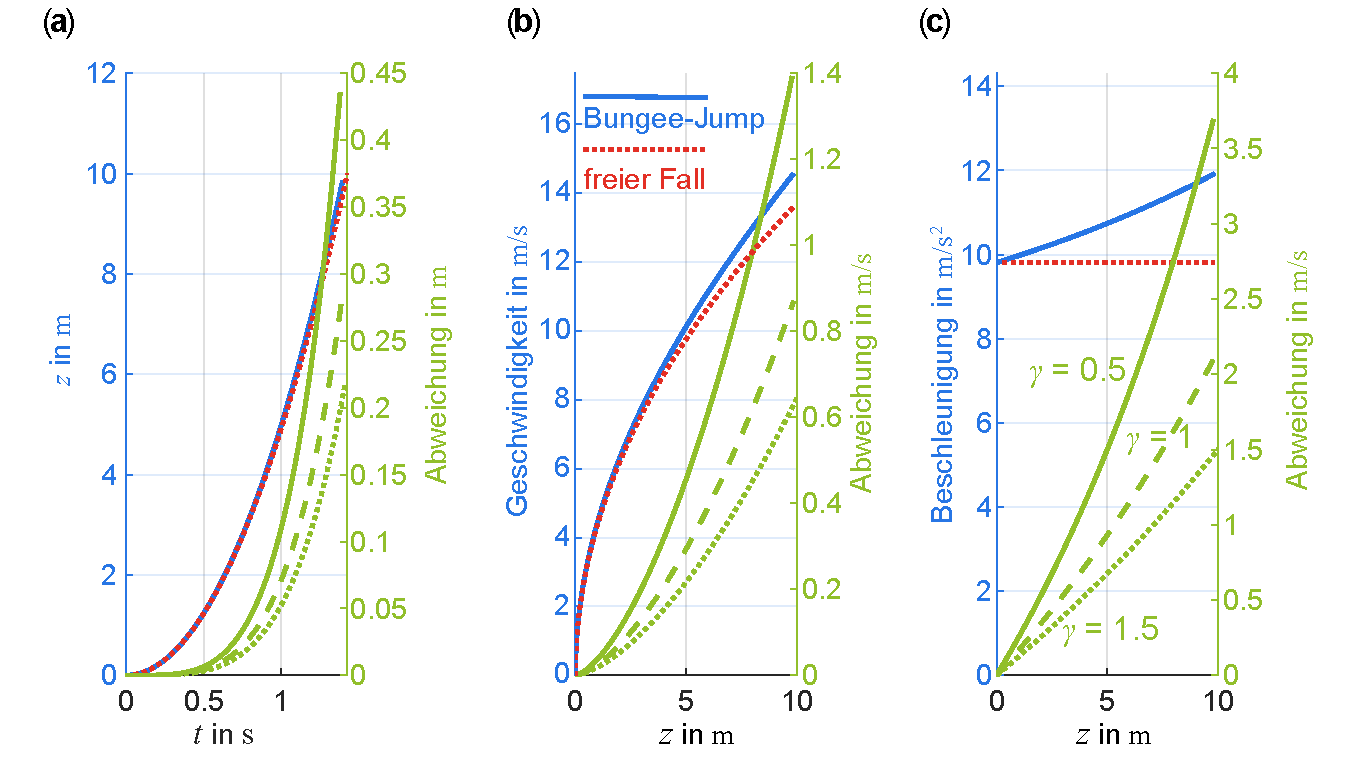
\includegraphics[width=\textwidth]{FallingChain03.pdf}
\caption[Dynamik des Bungee Jumping.]{%
Dynamik des Bungee Jumping. Parameter: Volle Seill�nge  $l_\text{K}=\SI{20}{\metre}$.
\fa Durchlaufene Fallstrecke als Funktion der Zeit.
Der \anf{Zuwachs} an Fallstrecke gegen�ber dem freien fall ist relativ gering und umso gr��er, je schwerer das Seil im Vergleich zum fallenden K�rper ist.
\fb Die analoge Darstellung f�r die Fallgeschwindigkeit.
Auch hier der Unterschied zum freien Fall sichtbar gr��er, je schwerer das Seil im Vergleich zum fallenden K�rper ist.
\fc Beschleunigung als Funktion der durchlaufenen Fallstrecke.
Man erkennt in der Abweichung $a\lk z\rk -g $ sehr sch�n, dass am Ende der Fallstrecke eine deutliche gr��ere Beschleunigung als $g$ auf den K�rper wirkt.}
\label{abb:bew_Bungee01}
\end{figure}

In \figref{bew_Bungee01} ist die Funktion $z\lk t\rk$ f�r den Bungee-Jumper f�r verschiedene Parameters�tze $q = m_\text{K}/m$
im Vergleich zum freien Fall dargestellt (\mscr{} \mlbewref{BungeeJumping.m}).
Man erkennt, dass in der Tat erhebliche gr��ere Beschleunigungen als $g$ auftreten k�nnen.
Wir wollen allerdings darauf hinweisen, dass wir in unserem Modell Energieerhaltung angenommen haben ($U_0 = T_\text{final}$),
was bei realen B�ndern nicht unbedingt gegeben sein muss. Au�erdem haben wir nicht ber�cksichtigt, dass bei Erreichen von $z=l_\text{K}$ das Band/Seil hinreichend elastisch sein sollte, damit der Springer vor Verletzungen gesch�tzt ist.

\subparagraph {\textbf{Enterhaken, Harpune}} 

Mit dem Problem des Bungee-Jumping eng verwandte Probleme sind das Werfen eines Enterhakens \cite{Mungan2022}, das Abschie�en einer Harpune oder das Werfen eines Lassos/Anlegetaus. Im Prinzip ist dies die Umkehrung des Bungee-Jumpings bzw. der fallenden Kette, wobei die geworfene Kette hier wieder die zus�tzliche Masse $m_\text{K}$ am Ende tragen kann (\figref{bew_FallingChain01}b). Wir k�nnen die Lagrange-Funktion schreiben als: 
        \begin{align}
            \mathcal{L} = \frac{M}{2}\,\dot{z}^2 - \frac{z^2}{2}\,g\,\mu\,. \label{eq:bew_Harpune01}
        \end{align}
Hierin haben wir einfacherweise  die Abschussrichtung $z$ senkrecht nach oben gew�hlt, $\mu$ ist wieder die Massendichte des Seils in $\SI{}{\g\per\cm}$, $M = m_\text{K}+\mu\,z$ die Gesamtmasse mit $m_\text{K}$ der Hakenmasse. Aus \eqref{eq:bew_Harpune01} folgt die Lagrange-Gleichung
        \begin{align}
            \lk m_\text{K} +\mu\,z\rk\,\ddot{z} + \mu\,\dot{z}^2 + \lk m_\text{K} + \mu\,z\rk\,g = 0\,, \label{eq:bew_Harpune02}
        \end{align}
was auch mit $P = M\,v$ einfach geschrieben werden kann als 
        \begin{align}
            \frac{\D P}{\D t} = \frac{\D}{\D t}\,\lk M\,v\rk = -M\,g ~~~~ \text{mit} ~~~~ v=\dot{z}\,. \label{eq:bew_Harpune03}
        \end{align}
Diese Gleichung kann nach der Geschwindigkeit $v$ als Funktion der H�he $z$ gel�st werden.
        \begin{align}
            \frac{\D P}{\D t} &= \frac{\D P}{\D z}\,\frac{\D z}{\D t}  = \frac{\D P}{\D z} \,\frac{P}{M}\,= -M\,g  \, \nonumber \\
            \rightarrow ~~~~ -P\,\D P &= g\,M^2\,\D z = g\,\lk m_\text{K} + \mu\,z\rk^2\,\D z \,.  \label{eq:bew_Harpune04a}
			  \end{align}
Integration von \eqref{eq:bew_Harpune04a} ergibt 
        \begin{align}
            m_\text{K}\,{v_0}^2 - M\,v^2 &= \frac{2g}{3\mu}\,\lk M^3-m_\text{K}\rk \nonumber \\
            \rightarrow ~~~~ v &= \lk 1+ \frac{\mu\,z}{m_\text{K}}\rk^{-1}\,\sqrt{{v_0}^2 - \frac{2m_\text{K}\,g}{3\mu}\,\lek\lk 1+\frac{\mu\,z}{m_\text{K}}\rk^3-1\rek} \,. \label{eq:bew_Harpune04b}
        \end{align}
F�r $v=0$ ergibt sich die maximale H�he
        \begin{align}
            z_\text{max} = \frac{m_\text{K}}{\mu}\,\lek\lk 1+ \frac{3\mu\,{v_0}^2}{2m_\text{K}\,g}\rk^{-\frac{1}{3}}-1\rek \,, \label{eq:bew_Harpune05}
        \end{align}
was f�r $\mu\rightarrow0$ in $z_{\text{max},\mu=0} = {v_0}^2/2g $ f�r den senkrechten Wurf nach oben �bergeht. \\
In \figref{bew_Harpune01} ist die Funktion $z\lk t\rk$ f�r verschiedene Parameters�tze
im Vergleich zum senkrechten Wurf nach oben dargestellt (\mscr{} \mlbewref{Harpune.m}).
F�r $m_\text{K} \rightarrow 0$ wird der Grenz�bergang dem Leser zur �bung empfohlen.
Etwas schwieriger ist die Behandlung des schr�gen Wurfs einer Kette oder einen Taus,
da wir dann ein komplexeres zweidimensionales Problem zu l�sen haben.
Auch dies empfehlen wir dem Leser in \probref{bew_Zusatz_KetteTau} zu untersuchen.
Ein Ansatz besteht darin, die Kette in der $x$-$z$-Ebene zu jedem Zeitpunkt als quasi statische Kettenlinie
unter dem Einfluss der Schwerkraft zu betrachten, deren L�nge und Endpunkt sich zeitlich ver�ndert.

\begin{figure}
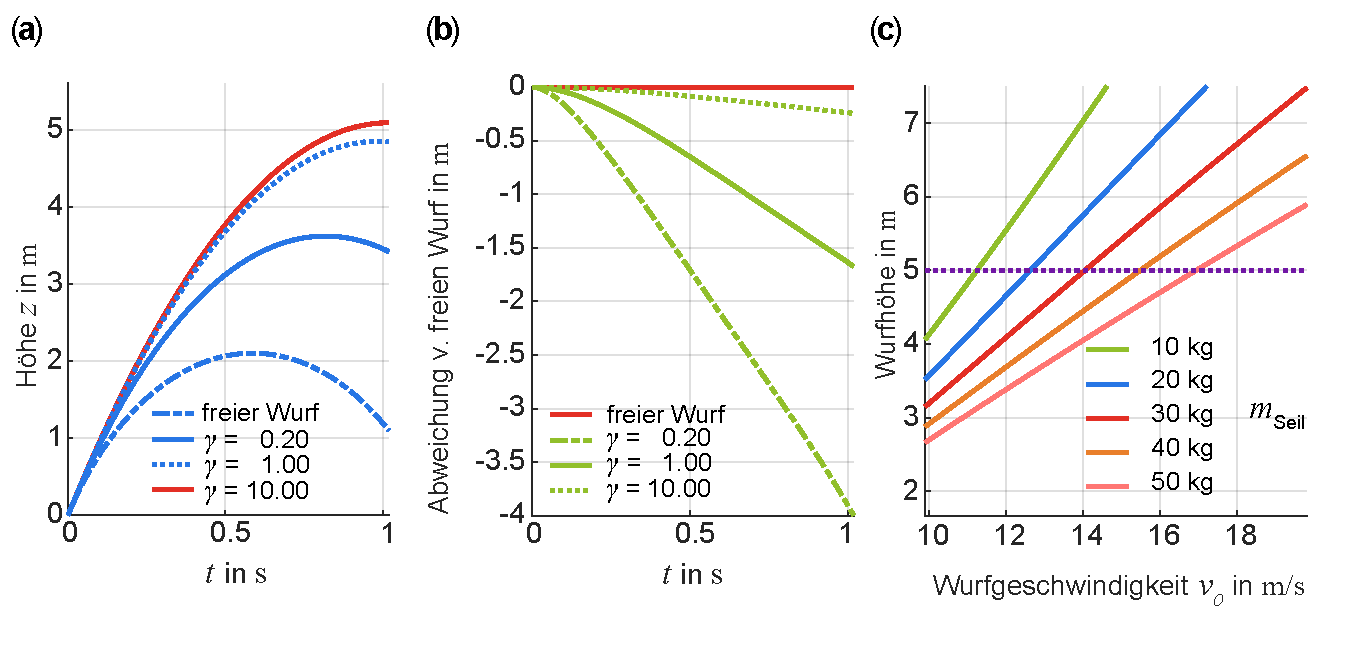
\includegraphics[width=\textwidth]{FallingChain04.pdf}
\caption[Dynamik eines Enterhakens/einer Harpune.]{Dynamik eines Enterhakens/einer Harpune. \fa Dargestellt ist die Funktion $z\lk t\rk$ f�r verschiedene Massenverh�ltnisse $\gamma = m_\text{Seil}/m_\text{K}$. Wie zu erwarten n�hert sich mit geringerer Seilmasse die Bewegung dem freien Wurf, denn wir nehmen unabh�ngig von der Gesamtmasse immer die gleiche Abwurfgeschwindigkeit an. \fb Abweichung vom freien Wurf. \fc Erreichbare Maximalh�he als Funktion der Abwurfgeschwindigkeit $v_0$ f�r verschiedene Seilmassen. Die Ankermasse (bzw. die Masse des geworfenen Tauendes ist immer $\SI{7.5}{\kg}$.}\label{abb:bew_Harpune01}
\end{figure}

Wer schon einmal am Meer beobachtet hat, wie Seeleute Taue (noch dazu nasse) beim Anlegen �ber $\approx 5$ bis $\SI{10}{\metre}$ werfen, kann nun eine Absch�tzung der Anfangsgeschwindigkeit und der dazu notwendigen Kraft machen. 
Wir wollen folgende Parameter annehmen:
	\[ m_\text{K} = \SI{7.5}{\kg} \;,~~l_\text{K} = \SI{25}{\metre}\;,~~\Delta t \approx \SI{0.2}{\s}\,,~~\Delta H = \SI{5}{\metre} \;.
	\]
Man berechnet daraus leicht Anfangsgeschwindigkeiten $v_0$ von $ \SI{11}{\metre\per\s} - \SI{18}{\metre\per\s}$ und notwendige Kr�fte $F \approx \SI{150}{\N} - \SI{650}{\N}$

\subparagraph{\textbf{Kettenfont�ne}} \index{Kettenfont�ne}

Eine besonders interessante Auspr�gung der Kettenproblematik ist die sogenannte Kettenfont�ne (\figref{bew_FallingChain01}c). Diese entsteht als Folge des nach seinem Entdecker Steve Mould\footnote{Steve Mould (geb. 1978) ist ein britischer \anf{Bildungs-Youtuber} und Wissenschaftskommunikator, der seine Wissenschaftspr�sentationen vorwiegend im Internet bringt.}\indexp{Mould, Steve} benannten Mould-Effekts, wenn eine Kette oder ein Seil aus einem Gef�� �ber den Rand nach unten gleitet. Das fallende Kettenende zieht dabei die im Gef�� liegenden Kettenglieder immer schneller nach. Der scharfe Knick, mit dem die Kette zun�chst �ber den Rand des Gef��es l�uft, weitet sich zu einem Bogen, der irgendwann den Rand nicht mehr ber�hrt, die Kette steigt zitternd in die H�he und l�st sich weiter aus dem Kn�uel. Sobald das fallende Ende den Boden erreicht, nehmen die Geschwindigkeit der Kette und damit auch die H�he der Font�ne nicht mehr weiter zu, ein station�rer Zustand ist erreicht. Im Internet sind auch zahlreiche Videos zu finden (\ua \url{https://www.youtube.com/watch?v=_dQJBBklpQQ}).\\
F�r die physikalische Erkl�rung der Entstehung des Bogens muss zus�tzlich zur Zugkraft der fallenden Kette eine weitere Kraft vorhanden sein. Diese Kraft muss aus der Energie/dem Impuls resultieren, die die Zugkraft der fallenden Kette in den Teil der Kette einbringt, der noch im Gef�� liegt \cite{Pantaleone2017}.
Die entstehende Form des Bogens l�sst sich im quasi-station�ren Zustand als eine umgekehrte Kettenlinie \index{Kettenlinie} beschreiben. Entlang dieser Kurve �ndert der Impuls kontinuierlich seine Richtung, w�hrend der Betrag (mit der L�ngsgeschwindigkeit) konstant bleibt. Die vektorielle Impuls�nderung wird gemeinsam bewirkt durch die Fallbeschleunigung einerseits und die Zugspannung in Kombination mit der Kr�mmung andererseits.\\
Wir wollen im Folgenden zun�chst ein einfaches Modell der Kettenfont�ne betrachten, welches erlaubt, die H�he der Kettenkurve �ber dem Gef�� zu berechnen und folgen hierbei der Darstellung den Autoren Biggins und Warner, die in \cite{Biggins2013, Biggins2014} erstmals eine mathematisch-physikalische Beschreibung des Ph�nomens gegeben haben.
\begin{figure}
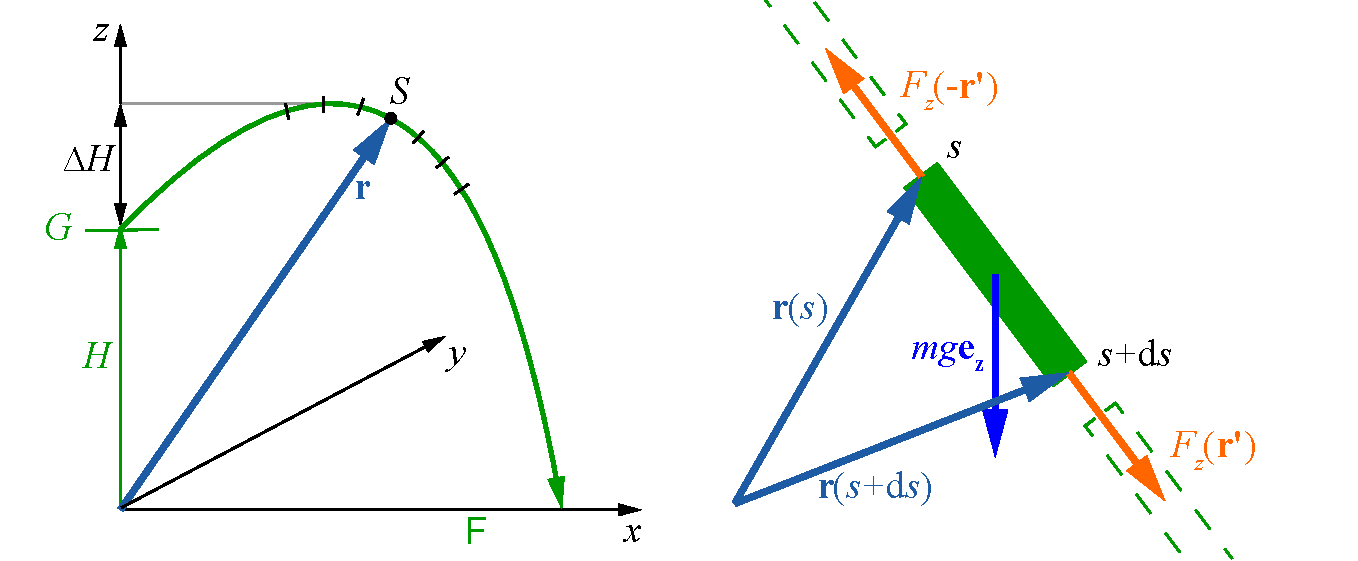
\includegraphics[width=\textwidth]{ChainFountain02.pdf}
\caption[Koordinaten und physikalische Gr��en der Kettenfont�ne.]{Koordinaten und physikalische Gr��en der Kettenfont�ne.}\label{abb:bew_chainfountain02}
\end{figure}

Wir wollen die Kette zun�chst als ein d�nnes, flexibles Seil mit konstanter L�nge annehmen.\footnote{Wir werden sp�ter sehen, dass wir zur Erkl�rung des Kettenfont�nen-Ph�nomens die Kette in diskrete Elemente \glqq zerlegen \grqq{} m�ssen.} Wir w�hlen $s$ als die L�ngengr��e entlang der Kette (\figref{bew_chainfountain02}a). Dann ist
\begin{align*}
        \vec{r}\lk s,t\rk & - \text{der Ortsvektor zur Zeit}~t~ \text{(zu einem bestimmten Punkt/Element der Kette) und} \\
        \vec{r}' = \d \vec{r}/ \d s  & - \text{der tangentiale Einheitsvektor an die Kette bei} ~ \vec{r}\lk s\rk ~\text{zur Zeit}~ t~ \\
				& \quad \text{mit} ~\vec{r}'\cdot\vec{r}' =1\,.
\end{align*} 
Wir k�nnen nun f�r ein Kettenelement $s+\D\,s$ die Newtonsche Bewegungsgleichung aufschreiben (\figref{bew_chainfountain02}b). $F_\text{Z}$ sei der Betrag der Zugkraft in der Kette (interne Spannkraft). Dann gilt:
\begin{align}
    F_\text{Z}\,\vec{r}'\big|_{s+\D s} -  F_\text{Z}\,\vec{r}'\big|_{s}  - \D m\,g\,\veceZ = \D m\,\frac{\d^2\vec{r}}{\d t^2}\,. \label{eq:bew_chainfountain01}
\end{align}
Wir f�hren die Gr��e $\mu$ als Masse pro L�nge ein ($\D m = \mu\,\D s$) und erhalten:
\begin{align}
    \frac{\d \lk F_\text{Z}\,\vec{r}'\rk}{\d s} =  \lk F_\text{Z}\,\vec{r}'\rk' = \mu\,\ddot{\vec{r}} +  \mu\,g\,\veceZ \,. \label{eq:bew_chainfountain02}
\end{align}
Der Strich bezeichnet hier eine Ableitung nach $s$. Wir wollen unter der Annahme \bzw Beobachtung, dass die Form der Font�ne zumindest f�r gewisse Zeiten relativ stabil ist, nach einer \emph{station�ren} L�sung suchen, also nach einer Kettenform $\vec{r}\lk s\rk$, die konstant in der Zeit ist, sich aber mit einer konstanten Geschwindigkeit $v$ entlang ihrer eigenen L�nge bewegen kann. Die Geschwindigkeit $v$ ist dann durch
\begin{align}
    v=\frac{\D s}{\D t} = \text{const} \label{eq:bew_chainfountain03}
\end{align}
definiert (\figref{bew_chainfountain02}c). Wir bilden:
\begin{align*}
    \vec{r}\lk t+\D\,t,s\rk &= \vec{r}\lk t,s + v\D\,t\rk \\
    \killB{\vec{r}\lk t\rk} + \frac{\d}{\d t}\vec{r}\D t + \killA{\mathcal{O}\lk \D t^2\rk} &= \killB{\vec{r}\lk t\rk} + \frac{\d}{\d s}\vec{r} \,v\D t + \killA{\mathcal{O}\lk \D t^2\rk}
\end{align*}
\begin{align}
\begin{split}
    \rightarrow ~~~~ \dot{\vec{r}} &= v \,\vec{r}'\,\\
    \rightarrow ~~~~ \ddot{\vec{r}} &= v\,\dot{\vec{r}}' = v^2\,\vec{r}''\,. 
\end{split} \label{eq:bew_chainfountain04}
\end{align}
Wir k�nnen dieses Ergebnis in \eqref{eq:bew_chainfountain02} einsetzen und erhalten:
\begin{align}
    \lk F_\text{Z}\,\vec{r}'\rk' - \mu\,g\,\veceZ = \mu\,v^2\,\vec{r}''\,. \label{eq:bew_chainfountain05}
\end{align}
Damit haben wir eine gew�hnliche DGL 2.~Ordnung f�r $\vec{r}\lk s\rk$ bekommen, die uns eine \emph{station�re} L�sung f�r die Kettenfont�ne gibt. In dieser Gleichung sind die innere Zugkraft $F_\text{Z}$ und die Geschwindigkeit $v$ noch unbekannte Parameter. Wir integrieren \eqref{eq:bew_chainfountain05} �ber $\D s$ und erhalten:
\begin{align}
    F_\text{Z}\,\vec{r}' - \mu\,g\,s\,\veceZ = \mu\,v^2\,\vec{r}' - \mu\,g\,\vec{C}\,. \label{eq:bew_chainfountain06}
\end{align}
Hierbei haben wir die Integrationskonstante $\vec{C}$ (ein Vektor!) aus im Folgenden verst�ndlichen Gr�nden mit $-\mu\,g$ multipliziert. \\
Wir formen \eqref{eq:bew_chainfountain06} um:
\begin{align}
    \lk F_\text{Z} - \mu\,v^2\rk\,\vec{r}' &= \mu\,g\,\lk s\,\veceZ-\vec{C}\rk  \nonumber \\
    \rightarrow ~~~\lk F_\text{Z} - \mu\,v^2\rk^2 &= \mu^2\,g^2\,\lk s\,\veceZ - \vec{C}\rk^2\,, \nonumber \\
    \rightarrow ~~~~ F_\text{Z} - \mu \,v^2 &= \pm\, \mu\,g\,\big| s\,\veceZ - \vec{C}\big|\,. \label{eq:bew_chainfountain07}
\end{align}
Wir multiplizieren \eqref{eq:bew_chainfountain07} mit $\vec{r}'$ und setzen $\lambda = \pm 1$:
\begin{align*}
    \lambda\,\mu\,g\,\big| s\,\veceZ - \vec{C}\big|\,\vec{r}' = \lk F_\text{Z} - \mu\,v^2\rk\,\vec{r}' = \mu\,g\,\lk s\,\veceZ - \vec{C}\rk \,,
\end{align*}
woraus
\begin{align}
  \vec{r}' = \lambda \,\frac{s\,\veceZ - \vec{C}}{\big| s\,\veceZ - \vec{C}\big|}\label{eq:bew_chainfountain08}
\end{align}
folgt. $\vec{r}'$ ist ein Einheitsvektor, was \eqref{eq:bew_chainfountain08} noch mal best�tigt. Haben wir einen Fortschritt gemacht? Schon! Wir haben eine DGL 2.Ordnung f�r $r\lk s\rk$ auf eine DGL erster Ordnung zur�ck gef�hrt und daf�r eine Integrationskonstante $\vec{C}$ (einen Vektor) erhalten, den es zu bestimmen gilt. \\
Wir vereinfachen uns das Problem etwas, indem wir annehmen, dass sich die Kettenfont�ne in der $x$-$z$-Ebene bildet. Dann kann man \eqref{eq:bew_chainfountain08} in Komponenten schreiben $\lk \vec{r} = \lk x,y,z\rk = \lk x,0,z\rk,~~ \vec{C} = \lk C_\text{x},C_\text{y},C_\text{z}\rk \rk$:
\begin{align}
    x' = \frac{\lambda\,\lk -\,C_\text{x}\rk}{\sqrt{C_\text{x}{}^2 + \lk s-C_\text{z}\rk^2}} \; , ~~~~~~~~ z' = \frac{\lambda\,\lk s-C_\text{x}\rk}{\sqrt{C_\text{x}{}^2 + \lk s-C_\text{z}\rk^2}} \label{eq:bew_chainfountain09}
\end{align}
Wir suchen ja eine L�sung f�r eine Kettenform, die einen Bogen mit �ffnung nach unten beschreibt, deswegen muss $\lambda = -1$ sein, wie man durch Bildung von $\d z'/\d s$ leicht nachrechnen kann. Die Gleichungen \eqref{eq:bew_chainfountain09} mit $\lambda = -1$ beschreiben mit $s$ als Parameter die station�re L�sung der Kettenfont�ne, allerdings noch in der Ableitung nach $s$. Wir integrieren deshalb �ber $\D s$ und erhalten:
\begin{align}
\begin{split}
    x\lk s\rk &= \ln\lek \frac{\sqrt{C_\text{x}{}^2 + \lk C_\text{z}-s\rk^2} -C_\text{z} + s}{\sqrt{C_\text{x}{}^2 + C_\text{z}{}^2} -C_\text{z}} \rek \; , \\
    z\lk s\rk &= H+ \sqrt{C_\text{x}{}^2 + C_\text{z}{}^2} - \sqrt{C_\text{x}{}^2 + \lk C_\text{z}-s\rk^2}\,,
\end{split} \label{eq:bew_chainfountain10}
\end{align}
mit den Randbedingungen  $x\lk 0\rk= 0$ und $z\lk 0\rk = H$ (H�he des Gef��bodens). \\
Wir haben jetzt mit \eqref{eq:bew_chainfountain10} die Form der Kettenfont�ne als Funktion von drei Parametern $C_\text{x}$, $C_\text{z}$ und $s$. Die beiden Gleichungen beschreiben eine Art Kettenlinie. Wir wollen nun die Parameter $C_\text{x}$, $C_\text{z}$ in Beziehung zu messbaren Gr��en setzen. \\
In \eqref{eq:bew_chainfountain07} hatten wir gefunden:
\begin{align}
    F_\text{Z} =  \mu \,v^2 \pm \mu\,g\,\big| s\,\veceZ - \vec{C}\big|\,, \label{eq:bew_chainfountain11}
\end{align}
woraus wir mit $z\lk s\rk$ aus \eqref{eq:bew_chainfountain10} f�r $\lambda = -1$
\begin{align}
    F_\text{Z}\lk s\rk = \mu\,v^2 - \mu\,g\,\lk z-H\rk - \mu\,g\,\sqrt{C_\text{x}{}^2 +C_\text{z}{}^2} \label{eq:bew_chainfountain12}
\end{align}
erhalten. Auch in dieser Darstellung $F_\text{Z}\lk z\rk$ haben wir drei unbekannte Parameter $v,C_\text{x},C_\text{z}$. Wir brauchen also Informationen �ber das System (Randbedingungen oder �hnliches), um diese freien Parameter zu bestimmen. 

\begin{figure}
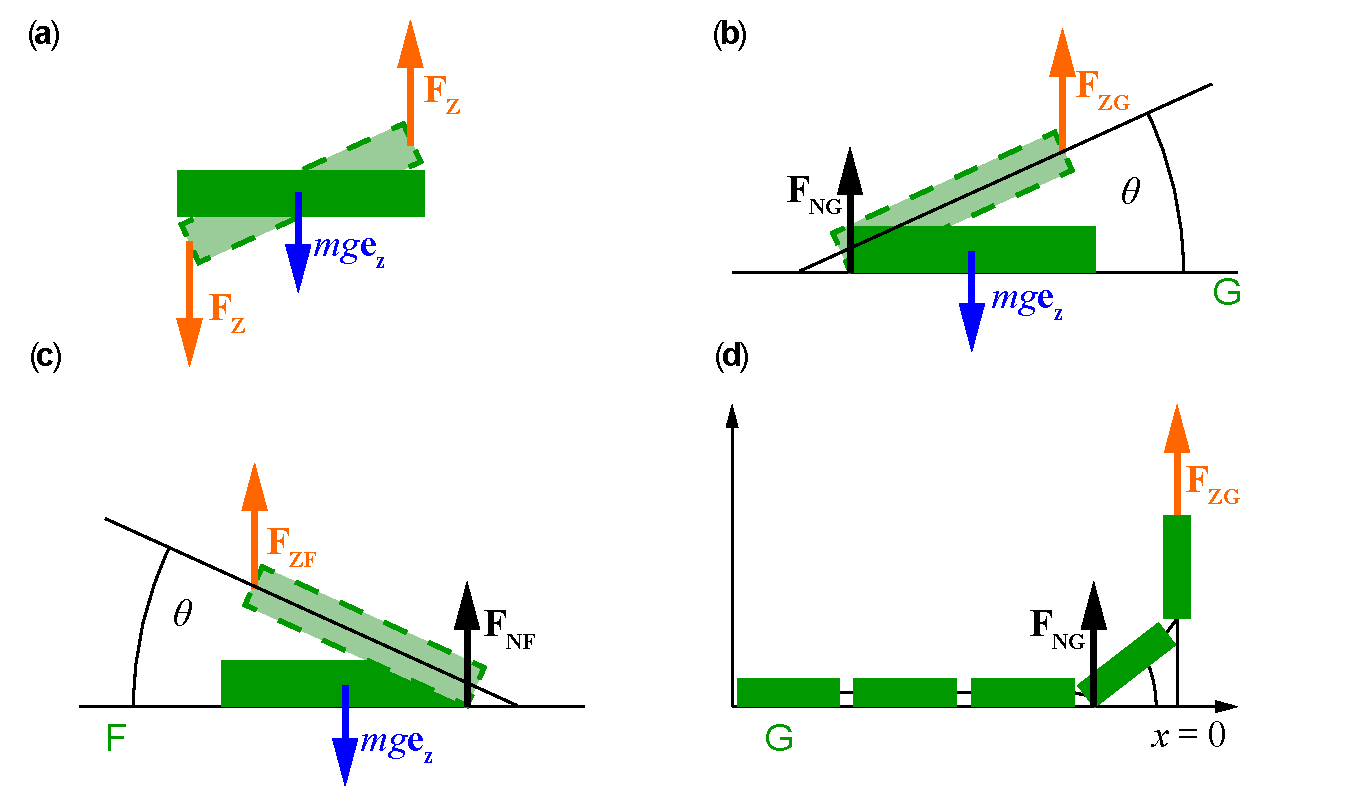
\includegraphics[width=\textwidth]{ChainFountain02a.pdf}
\caption[Kr�fte an den Kettengliedern einer Kettenfont�ne.]{Kr�fte an den Kettengliedern einer Kettenfont�ne. \fa Ein Kettenglied, das nicht auf einer Unterlage aufliegt, wird sich um seinen Schwerpunkt drehen. \fb Kr�fte bei einem abhebenden Kettenglied auf dem Gef��boden. \fc Kr�fte bei einem auftreffenden Kettenglied auf dem Fu�boden. \fd Winkel beim Abheben eines Kettengliedes.} \label{abb:bew_chainfountain02a}
\end{figure}

An dieser Stelle m�ssen wir nun das einfache Modell des Seil verlassen und ein Modell der Kette mit diskreten, als stabf�rmig angenommenen Kettengliedern benutzen. Wir betrachten \figref{bew_chainfountain02a}b und schreiben zun�chst die Newtonsche Bewegungsgleichung f�r ein einzelnes Kettenglied auf, das sich in der N�he des Gef��bodens (G)
befindet:
\begin{align*}
    F_\text{N,G} = m\,g + F_\text{Z,G} = \mu\,l_\text{K}\,\frac{\Delta v}{l_\text{K}/\Delta v} \approx \mu\,v^2 \,.
\end{align*}
Hier ist $F_\text{N,G}$ eine Normalkraft des Gef��bodens und $F_\text{Z,G}$ die wirkende Zugkraft in dem Kettenglied, das sich gerade vom Boden des Gef��es l�st. Da f�r ein einzelnes Kettenglied $m\,g = \mu\,l_\text{K}\,g$ sehr klein ist, k�nnen wir n�herungsweise schreiben
\begin{align}
    F_\text{Z,G} + F_\text{N,G} \approx \mu\,v^2 \label{eq:bew_chainfountain13a}
\end{align}
und analog f�r den Fu�boden (F):
\begin{align}
     F_\text{Z,F} +  F_\text{N,F} \approx \mu\,v^2 \,. \label{eq:bew_chainfountain13b} 
\end{align}
In \eqref{eq:bew_chainfountain13a} und \eqref{eq:bew_chainfountain13b} sind:
	\[	F_\text{Z,G} =  F_\text{Z}\lk H\rk ~~~~ \text{und} ~~~~  F_\text{Z,F} =  F_\text{Z}\lk 0\rk\,.\]
Wir setzen nun \eqref{eq:bew_chainfountain12} in \eqref{eq:bew_chainfountain13a} ein und erhalten
\begin{align*}
    -\mu\,g\,\sqrt{C_\text{x}{}^2 +C_\text{z}{}^2} + F_\text{N,G} = 0\,,\\
    -\mu\,g\,H - \mu\,g\,\sqrt{C_\text{x}{}^2 +C_\text{z}{}^2} + F_\text{N,F} = 0\,,
\end{align*}
woraus folgt $F_\text{N,G}>0$. \\
Warum �bt der Boden des Gef��es eine Normalkraft in positive $z$-Richtung auf die Kette aus? Das erscheint zun�chst paradox. F�r den Moment des Abhebens schauen wir uns die Newtonsche Bewegungsgleichung f�r die $z$- und die $\theta$-Koordinate genauer an\footnote{Die Gleichung f�r die $\theta$-Koordinate entspricht der Drehmomentbilanz (\kap{bew_Drehimpuls_StarrerK}).} (\figref{bew_chainfountain02a}b):
\begin{align}
\begin{split}
    F_\text{N,G} + F_\text{Z,G} -m\,g &= m\,\ddot{z}\,, \\
    F_\text{Z,G} \,\frac{l_\text{K}}{2}\,\cos\theta - F_\text{N,G}\,\frac{l_\text{K}}{2}\,\cos\theta &= J\,\ddot{\theta}\,. \label{eq:bew_chainfountain14}
\end{split}
\end{align}
Hierin ist $J$ das Tr�gheitsmoment des Kettengliedes bez�glich seines Schwerpunktes (\kap{bew_Drehimpuls_StarrerK}).
DGL-System \eqref{eq:bew_chainfountain14} kann numerisch gel�st werden.
Wir wollen uns aber vorerst die lineare N�herung f�r kleine Winkel anschauen, wohl wissend, dass $\theta$ auch gro�e Werte annehmen kann. Wir werden diese N�herung deshalb auch gleich wieder fallen lassen, k�nnen aber zun�chst mit $\cos\theta \approx 0$ und $z\approx (l_\text{K}\,\theta )/ 2$ schreiben:
\begin{align}
\begin{split}
    F_\text{Z,G} + F_\text{N,G}  - m\,g &= m\,\ddot{z} \approx m\,\frac{v^2}{l_\text{K}}\,,\\
    \frac{l_\text{K}}{2}\,F_\text{Z,G} - F_\text{N,G} \,\frac{l_\text{K}}{2} &= 2J\,\ddot{\theta}\,. \label{eq:bew_chainfountain15}
\end{split}
\end{align}
Wir k�nnen nun aus \eqref{eq:bew_chainfountain15} $F_\text{Z,G}$ eliminieren und erhalten mit $J=\frac{1}{12}\,m\,l_\text{K}^2$ f�r einen homogenen Stab und $m\,g \ll F_\text{Z,G},F_\text{N,G}  $:
\begin{align}
    F_\text{N,G} = \frac{1}{2}\,\lk m-\frac{4J}{l_\text{K}^2}\rk\,\frac{v^2}{l_\text{K}} = \frac{1}{3}\,m\,\frac{v^2}{l_\text{K}} = \frac{1}{3}\,\mu\,v^2 \,.  \label{eq:bew_chainfountain16}
\end{align}
Wir erinnern uns, dass $F_\text{N,G}$ nach \eqref{eq:bew_chainfountain16} der Bedingung kleine Winkel hergeleitet wurde, deswegen schreiben wir zur Ber�cksichtigung gr��erer Winkel besser verallgemeinert
\begin{align}
    F_\text{N,G} = \alpha \,\mu\,v^2 \,, \label{eq:bew_chainfountain17}
\end{align}
worin $\alpha$ eine gegebenenfalls numerisch oder experimentell zu bestimmende Konstante des Systems ist.\footnote{Die Proportionalit�t ist eine Annahme, die durch das Experiment verifiziert werden kann.} \\
V�llig analog kann man die Situation beim Auftreffen auf dem Fu�boden beschreiben und wir finden dann f�r die entsprechende Normalkraft (\figref{bew_chainfountain02a}c):
\begin{align}
    F_\text{N,F} = \lk 1-\beta\rk\,\mu\,v^2 \,,\label{eq:bew_chainfountain18}
\end{align}
worin $\beta$ wieder eine experimentell bzw. numerisch zu bestimmende Konstante ist. Experimentell findet man Werte von $\alpha\approx\SI{0.12}{}$ und $\beta \leq \SI{0.1}{}$. 
Damit k�nnen wir nun auch die Zugkr�fte in der Kette im Gef�� und auf dem Fu�boden bestimmen:
\begin{align}
\begin{split}
    F_\text{Z,G} &= \mu\,g\,\sqrt{C_\text{x}{}^2 +C_\text{z}{}^2} = \alpha\,\mu\,v^2     \,,   \\
    F_\text{Z,F} &= \mu\,g\,\sqrt{C_\text{x}{}^2 +C_\text{z}{}^2} + \mu\,g\,H = \lk 1-\beta\rk\,\mu\,v^2\,. \label{eq:bew_chainfountain19}
\end{split}
\end{align}
Da $\alpha$ und $\beta$ jetzt bekannt \bzw experimentell bestimmt sind, bleibt $v$ als einzige Unbekannte. Diese k�nnen wir aus \eqref{eq:bew_chainfountain19} erhalten:
\begin{align}
   \killA{\mu}\,g\,H &= \lk 1-\alpha-\beta\rk\,\killA{\mu}\,v^2 ~~\rightarrow ~~ v = \sqrt{\frac{g\,H}{\lk 1-\alpha-\beta\rk}}\approx \sqrt{\frac{g\,H}{0.77}} \label{eq:bew_chainfountain20}
\end{align}
Entscheidend f�r die Entstehung einer Kettenfont�ne ist der Abstand zwischen Kettengliedern \bzw die L�nge der Verbindungsst�cken, die in jedem Fall so klein sein muss, dass das gerade abhebende Kettenglied beim Abheben nicht unter dem Winkel von $90\degree$ abheben kann. Interessant ist auch, dass die Fallgeschwindigkeit der Kettenfont�ne geringer ist als die Geschwindigkeit des freien Falls $\sqrt{2\,g\,H}$, was offensichtlich durch die wirkenden Normalkr�fte von Gef��- und Fu�boden zustande kommt. Wir kommen darauf noch einmal zur�ck. Setzen wir $v$ in die ersten Gleichung von \eqref{eq:bew_chainfountain19} ein, erhalten wir daraus eine Beziehung zwischen den Konstanten $C_\text{x}$ und $C_\text{z}$:
\begin{align}
    C_\text{x} = +\sqrt{\lek \frac{\alpha\,H}{\lk 1-\alpha-\beta\rk}\rek^2-C_\text{z}{}^2}\,. \label{eq:bew_chainfountain21}
\end{align}
Setzen wir diese in \eqref{eq:bew_chainfountain12} ein, finden wir f�r die Zugkraft:
\begin{align}
    F_\text{Z}\lk z\rk = \lambda\,g\,\lek z + \frac{\beta\,H}{1-\alpha-\beta}\rek = \lambda\,g\,\lek z + \frac{\beta \, \gamma}{\alpha}\rek ~~\text{mit}~~\gamma= \frac{\alpha\,H}{1-\alpha-\beta}\,.\label{eq:bew_chainfountain22}
\end{align}
Damit haben wir unser Ziel erreicht, und die Zugkraft $F_\text{Z}\lk z\rk$ als Funktion von bekannten geometrischen und physikalischen Parametern und der H�he $z$ �ber dem Fu�boden beschrieben. Damit k�nnen wir auch die Gleichungen der Kettenlinie in Parameterform von $s$, $\alpha$ und $\beta$ \bzw $\gamma$ schreiben:
%\begin{align*}
%\begin{split}
    %x\lk s\rk &= \sqrt{\lk \frac{\alpha\,H}{\lk 1-\alpha-\beta\rk}\rk^2 -C_\text{z}{}^2}\,\ln\lek\frac{\sqrt{\lk \frac{\alpha\,H}{\lk 1-\alpha-\beta\rk}\rk^2-2C_\text{z}\,s+s^2} - C_\text{z} + s}{\frac{\alpha\,H}{\lk 1-\alpha-\beta\rk} - C_\text{z}}\rek\,, \\
    %z\lk s\rk &= H + \frac{\alpha\,H}{\lk 1-\alpha-\beta\rk} - \sqrt{\lek \frac{\alpha\,H}{\lk 1-\alpha-\beta\rk}\rek^2 - 2C_\text{z}\,s + s^2} \,.
%\end{split} 
%\end{align*}
\begin{align}
\begin{split}
    x\lk s\rk &= \sqrt{\gamma^2 - C_\text{z}{}^2}\,\ln\lek\frac{\sqrt{\gamma^2-2C_\text{z}\,s+s^2} - C_\text{z} + s}{\gamma - C_\text{z}}\rek\,, \\
    z\lk s\rk &= H + \gamma - \sqrt{\gamma^2 - 2C_\text{z}\,s + s^2} \,.
\end{split} \label{eq:bew_chainfountain23}
\end{align}
Leider haben wir in diesen parametrisierten Gleichungen noch immer eine Unbekannte ($C_\text{z}$).
Wir brauchen also noch eine weitere Bedingung, um diese zu bestimmen 
und betrachten dazu einen Grenzfall f�r einen Impulseintrag aus dem Gef��,
n�mlich wenn das Kettenglied im Moment des Abhebens (\figref{bew_chainfountain02a}d) nahezu senkrecht steht. Dann m�sste gelten:
	\[z' = \frac{\d z}{\d s} \big|_0 \approx 1 ~~ \text{und}~~ x' = \frac{\d x}{\d s}\big|_0 \approx 0\,. \]
Setzen wir diese Grenzbedingungen in \eqref{eq:bew_chainfountain23} ein, k�nnen wir das noch fehlende Glied $C_\text{z}$ bestimmen und erhalten damit:
\begin{align}
\begin{split}
    C_\text{x} &= \gamma\, \\
    \rightarrow ~~ x\lk s\rk &= 0 \,~ \text{und} ~
    z\lk s\rk = \frac{\lk 1-\beta\rk\,H}{\lk 1-\alpha-\beta\rk} - \Bigg| \frac{\alpha\,H}{\lk 1-\alpha-\beta\rk} -s\Bigg| = \frac{1-\beta}{\alpha}\,\gamma - \Bigg| \gamma -s\Bigg| \,.
\end{split} \label{eq:bew_chainfountain24}
\end{align}
Offensichtlich beschreibt diese station�re L�sung eine in sich zur�cklaufende Kette, die bei $z_{\max} > H$ einen h�chsten Punkt erreicht:
\begin{align}
    z_{\max} &= \frac{\lk 1-\beta\rk\,H}{\lk 1-\alpha-\beta\rk} ~~\rightarrow ~~\Delta H &= z_{\max} - H = \frac{\alpha\,H}{\lk 1-\alpha-\beta\rk} \,.
\label{eq:bew_chainfountain25}
\end{align}
\figref{bew_chainfountain04}a zeigt berechnete Werte f�r $z_{\max}$ f�r verschiedene Parameter. Die Font�nenh�he $\Delta H$ h�ngt also von der Gef��h�he $H$ und dem Parameter $\alpha$ ab, weniger von $\beta$. Das ist nicht �berraschend, da die Font�nenh�he vom Impuls abh�ngt, der von der Unterlage auf die Kette �bertragen wird. Dieser h�ngt aber wiederum von der Geschwindigkeit der Kette ab, die aber als Wirkung aus der Gravitation von der H�he $H$ abh�ngt \eqref{eq:bew_chainfountain20}.\\
Offensichtlich folgt f�r $\alpha = 0,\, \beta = 0$ und $\Delta H=0$ dann $v^2 = H\,g$. Das ist der Fall einer frei fallenden Kette der L�nge $H$, den wir schon in \eqref{eq:bew_FallingChain05} berechnet hatten.\\
Nat�rlich kann in der Realit�t eine Kette nicht in sich (bei $x=0$) zur�ck laufen. Das �berraschende Ergebnis unseres Modells ist in zwei gemachten Annahmen begr�ndet. Zum einen hatten wir den Grenzfall $z' = \d z/\d s (0) \approx 1 $ angenommen und zum anderen stillschweigend eine unendlich d�nne Kette angenommen, bei der alle Kettenglieder bei $x=0$ vom Boden des Gef��es abheben. Beides sind in der Realit�t sicher nicht zutreffende Annahmen. Unser Modell liefert aber dennoch sehr realistische H�hen der Font�ne �ber dem Gef��.\\

Wir wollen zum Schluss noch die energetischen Verh�ltnisse und den Radius des Bogens der Kettenfont�ne betrachten. F�r das Verh�ltnis von kinetischer Energie der Kette zu potentieller Energie (pro L�ngeneinheit) finden wir:
\begin{align}
    \frac{T}{U} &= \frac{v^2/2}{g\,H} = \frac{1}{2}\frac{1}{ 1-\alpha-\beta}\,.
\label{eq:bew_chainfountain26}
\end{align}
Wiederum ergibt sich f�r $\alpha=\beta=0$ der Fall der frei fallenden Kette mit einem Energieverh�ltnis von 0.5 bei der Kettenfont�ne interessanterweise etwas weniger. Aus \eqref{eq:bew_chainfountain26} folgt auch, dass $\alpha+\beta \leq 0.5$ sein muss. 
%Bei $\alpha = 0.5$ und $\beta=0$ w�rde $\Delta H = H$ folgen und es g�be keine Energiedissipation. Das ist aber unrealistisch, weil die Parameter $\alpha$ und $\beta$ von vergleichbarer Gr��e sind (zur Berechnung von $\alpha$ siehe auch \cite{Biggins2013}).
Der sich ausbildende Bogen der Kette kann nur durch die Wirkung der Zugkraft als Radialkraft zustande kommen (wir nehmen wieder an $F_\text{Z,B} \gg m\,g$). Dann muss gelten (\figref{bew_FallingChain01}c):
\begin{align}
    \frac{F_\text{Z,B}}{R} &= \frac{\mu\,v^2}{R} \,.
\label{eq:bew_chainfountain27}
\end{align}
Interessanterweise k�rzt sich der Radius des Bogens heraus, was bedeutet, dass solange $v^2 \gg g\, R$ gilt es auch sehr, sehr enge Kurvenradien geben kann. Dies rechtfertigt nachtr�glich unsere Modellannahmen, bedeutet aber auch, dass das Modell keine Erkl�rung f�r den Radius des Bogens der Font�ne liefern kann. F�r weitergehende Betrachtungen empfehlen wir \cite{Biggins2013, Biggins2014, Pantaleone2017, Anghel2021}. \\

\begin{figure}
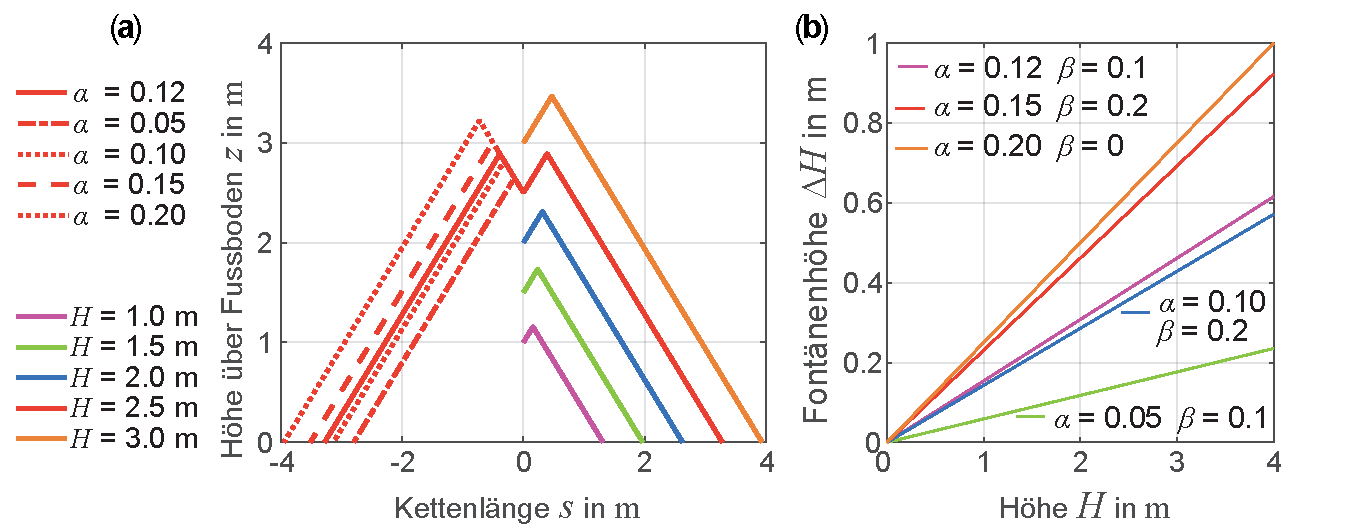
\includegraphics[width=\textwidth]{ChainFountain03.pdf}
\caption[H�he der Kettenfont�ne. ]{H�he der Kettenfont�ne �ber der Kettenl�nge $s$ als Funktion der Parameter $\alpha, \beta$ und $H$. Man beachte, dass im linken Bild $s$ keine kartesische Koordinate ist, sondern die L�nge entlang der Kette. $H$ ist die H�he des Gef��es �ber den Fu�boden.}\label{abb:bew_chainfountain04}
\end{figure}
Wir wollten mit diesem Kapitel zeigen, 
\begin{enumerate}
    \item [a)]
    dass man zur Beschreibung eines physikalischen Problems unter Umst�nden mehrere, z.T. sehr unterschiedliche Modelle braucht (in unserem Fall Kontinuum (Seil) und diskrete Elemente der Kette)
    \item [b)]
    dass es Sinn macht, auch bei einem dynamischen Problem nach einer quasi-station�ren L�sung zu suchen, 
    \item [c)]
    dass man alle denkbaren Rand- und Nebenbedingungen untersuchen muss, um Konstanten der Bewegung zu bestimmen, und
    %\item [e)]
    %dass es Systeme aus Massepunkten gibt, die obwohl es keinen Reibungsterm in den Bewegungsgleichungen gibt, zu Energiedissipation f�hren k�nnen, und  
    \item [d)]
    dass man die Wirkung von Normalkr�ften auf einen ausgedehnten K�rper nicht untersch�tzen darf.%
    \footnote{Wir werden entsprechende Effekte auch in \kap{bew_fallendeLeiter} wieder finden und auch n�her betrachten.}
\end{enumerate}


\clearpage
\section{Mechanik starrer K�rper}\label{kap:bew_starrer_koerper}
\index{K�rper!starrer}

Die vorherigen Abschnitte betrachteten nur Situationen, in denen ein K�rper
als Punktmasse behandelt werden konnte.
In vielen Anwendungen greift diese N�herung jedoch
zu kurz und muss die Ausdehnung des K�rpers explizit einbezogen
werden.
Das wollen wir in diesem Kapitel tun und dabei annehmen, dass
der K�rper w�hrend der gesamten Bewegung seine Form beh�lt, also nicht
deformierbar ist. 
Dies ist das Modell des starren K�rpers.

Ein starrer K�rper kann \zb aus einem System von $N$ diskreten Massepunkten
bestehen.
Dies haben wir bereits in \ref{kap:bew_basics_of_systems} betrachtet, sodass wir darauf Bezug nehmen k�nnen.
In den meisten F�llen l�sst sich ein starrer K�rper jedoch als eine kontinuierliche
Massenverteilung mit der Dichte $\varrho(\vec{r})$ betrachten, sodass wir das Konzept entsprechend erweitern.
Die
Gesamtmasse des K�rpers betr�gt dann
\begin{equation}
  M = \int_V \varrho(\vec{r}) \, \D^3 r  ~,
\end{equation}
wobei �ber sein gesamtes Volumen $V$ integriert wird.

Da der K�rper seine Gestalt nicht ver�ndert, ist es sinnvoll, zu seiner
Beschreibung zwei Koordinatensysteme einzuf�hren, ein raumfestes KOS $\vec{\Sigma}$ mit
den Standardachsen $\veceX$, $\veceY$ und $\veceZ$ und ein
k�rperfestes KOS $\vec{\Sigma}'$, dessen Achsen wir mit $\vecpeX$, $\vecpeY$ und
$\vecpeZ$ bezeichnen wollen und das seinen Ursprung im Schwerpunkt des
K�rpers hat (siehe \figref{bew_KOS_starrerKoerper}).

\begin{figure}
  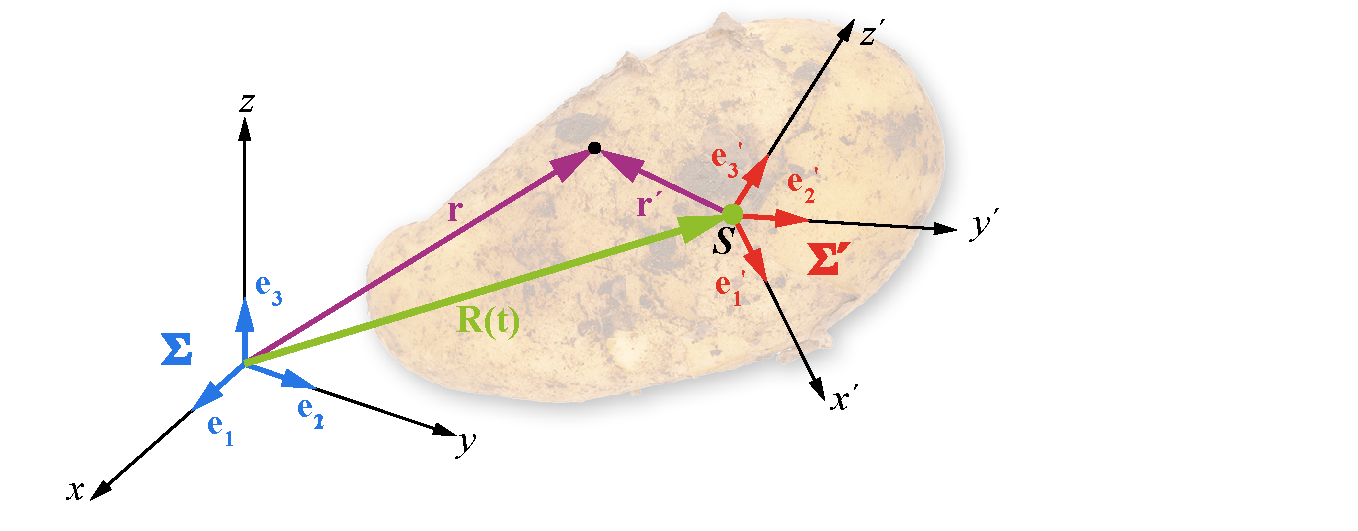
\includegraphics[width=\textwidth]{StarrKoerpKOS.pdf}
  \caption[Koordinatensysteme des starren K�rpers.]{Zur Beschreibung eines
    starren K�rpers ist es sinnvoll, ein raumfestes Koordinatensystem \index{Koordinatensystem!raumfestes} mit
    den Standardachsen  $\veceX$, $\veceY$ und $\veceZ$ sowie
    ein k�rperfestes\index{Koordinatensystem!k�rperfestes} mit den Achsen $\vecpeX$, $\vecpeY$ und
    $\vecpeZ$ heranzuziehen. Das k�rperfeste System hat seinen Ursprung
    im Schwerpunkt des K�rpers.}
    \label{abb:bew_KOS_starrerKoerper}
\end{figure}

Einen Vektor zu einem Punkt des K�rpers k�nnen wir somit im Koordinatensystem
$\vec{\Sigma}$ aus dem Schwerpunktsvektor $\vec{R}_S$ und einem Vektor $\vec{r'}$
aus dem k�rperfesten System $\vec{\Sigma}'$ mithilfe der entsprechenden Koordinatentransformation
zusammensetzen (siehe auch \kap{bew_rotating_systems}):
\begin{equation}
  \vec{r} = \vec{R}_S + \mathbb{R} \vec{r}' \,.
\end{equation}
Der Vektor $\vec{r}'$ zeigt vom Schwerpunkt zum Punkt im K�rper. 
Da er im k�rperfesten System gegeben ist, h�ngen seine Koordinaten nicht von der Zeit ab. Wir bezeichnen ihn im Folgenden mit $\vec{x}'$, um eine Verwechslung mit der Darstellung von $\vec{r}$ im k�rperfesten System $\vec{\Sigma}'$ zu vermeiden. Seine Darstellung im raumfesten System $\vec{\Sigma}$ nennen wir $\vec{x}$.


F�r die Geschwindigkeit dieses Punktes im raumfesten KOS folgt analog zu \kap{bew_rotating_systems}
\begin{equation}
  \vec{v} = \frac{\D}{\D t} \vec{r} = \vec{V}_S + \vec{\omega}' \times \vec{r}' = \vec{V}_S + \vec{\omega} \times \vec{x} \,,
  \label{eq:bew_Geschw_starrerK}
\end{equation}
mit der Schwerpunktgeschwindigkeit $\vec{V}_S$ und der momentanen Winkelgeschwindigkeit
$\vec{\omega}(t)$ der Drehbewegung des k�rperfesten Bezugssystems.

\subsection{Grundlagen der Kinematik}\index{Tr�gheitstensor}\index{Tr�gheitsmoment} \label{kap:bew_Kinematik_StarrerK}

\subsubsection{Kinetische Energie, Tr�gheitstensor und Tr�gheitsmoment}
\label{kap:bew_StarrerK_kin_Energie}

Die kinetische Energie eines starren K�rpers berechnet sich entsprechend Definition \eqref{eq:bew_Ges_Energie} unter Nutzung der Beziehung f�r die 
Geschwindigkeit \eqref{eq:bew_Geschw_starrerK} zu
\begin{align}
  T &= \frac{1}{2} \int_V \varrho(\vec{x}) \left ( \vec{V}_S
      + \vec{\omega} \times \vec{x} \right )^2 \, \D^3 x
      = \frac{1}{2} \int_V \varrho(\vec{x}) \left ( {\vec{V}_S}^2
      + (\vec{\omega} \times \vec{x})^2 \right ) \, \D^3 x \\
    &= \frac{1}{2} M\,{\vec{V}_S}^2 + \frac{1}{2} \int_V \varrho(\vec{x})
      (\vec{\omega} \times \vec{x})^2 \, \D^3 x
    = T_\mathrm{trans} + T_\mathrm{rot}\,.
      \label{eq:bew_Kin_Energie_starrerK}
\end{align}
Die kinetische Energie setzt sich aus einem Term $T_\mathrm{trans}$, der aus der Translation des Schwerpunkts
stammt, und der Rotationsenergie $T_\mathrm{rot}$ zusammen.
Der Mischterm aus dem ersten
Integral verschwindet, da in diesem $\vec{x}$ linear vorkommt und somit das Integral den
Schwerpunkt berechnet, der aber gerade den Wert $\vec{x} = \vec{0}$ hat.%
\footnote{Es gilt ja 
	$\int_V \varrho(\vec{x})\, \vec{x} \,\D^3 x = \vec{0}$.}

Die Rotationsenergie l�sst sich noch so umschreiben, dass wir die Eigenschaft
des K�rpers (seine Massenverteilung) von der Drehachse und der Winkelgeschwindigkeit trennen k�nnen.\footnote{$M$ bezeichnet hier die Gesamtmasse des starren K�rpers und man muss en bisschen aufpassen, dass man diese nicht mit dem Betrag des Drehmoments verwechselt, das wir \ia mit $\vec{M}_\text{D}$ bezeichnen. Wir werden auch bei den Beispielen zur besseren Eindeutigkeit die Massen h�ufig mit $m$ bezeichnen.}
Mit der Rechenregel $(\vec{a} \times \vec{b})^2 = \vec{a}^2 \vec{b}^2 - (\vec{a}\cdot \vec{b)^2}$ der Vektoralgebra (siehe die \onlineZ) folgt
\begin{equation}
  T_\mathrm{rot} = \frac{1}{2} \vec{\omega}^T \,\underline{\vec{\Theta}} \,\vec{\omega} = \frac{1}{2} \lk\omega_1\,,\omega_2\,,\omega_3\rk \,\underline{\vec{\Theta}} \,\lk\begin{array} {l} \omega_1\\\omega_2\\ \omega_3\end{array}\rk\,,
  \label{eq:bew_Trot_starrerK}
\end{equation}
worin $\underline{\vec{\Theta}}$ der \emph{Tr�gheitstensor}\footnote{%
In der linearen Algebra ist der Begriff des Tensors\index{Tensor} eine Verallgemeinerung des Begriffs der Matrix. 
Da wir hier keine weitergehende Theorie f�r Tensoren ben�tigen, k�nnen wir f�r unsere Zwecke die Begriffe Tensor und Matrix synonym verwenden. Zur Kennzeichnung eines Tensor benutzen wir \ia als Symbol einen unterstrichenen Vektor $\underline{\vec{A}}$ oder $\mathbb{A}$.  
F�r tiefergehende Betrachtungen sei auf \cite{Riley2006, Felder2016, Bartelmann2015} und \cite{Otto2019, Fischer2018} verwiesen.}
ist, der die Eigenschaften des K�rpers enth�lt und dessen Komponenten
\begin{subequations}
  \begin{align}
    \Theta_{ij} &= \int_V \varrho(\vec{x}) \left ( \vec{x}^2 \delta_{ij} -x_i x_j
    \right )\, \D^3 x  \\
    \intertext{\bzw ausgeschrieben}
    \underline{\vec{\Theta}} &= \begin{pmatrix} \Theta_{11}&\Theta_{12}&\Theta_{13}\\ \Theta_{21}&\Theta_{22}&\Theta_{23}\\ \Theta_{31}&\Theta_{32}&\Theta_{33}
    \end{pmatrix}
     = \bigintsss_V \varrho(\vec{x}) \begin{pmatrix} y^2+z^2 & -x\,y & -x\,z \\ -x\,y & x^2+z^2 & -y\,z \\ -x\,z & -y\,z & x^2+y^2 \end{pmatrix} \, \D^3 x \label{eq:bew_traegheitstensor}
  \end{align}
\end{subequations}
lauten. $\delta_{ij}$ ist das Kronecker-Symbol\index{Kronecker-Symbol}\indexp{Kronecker, Leopold}. Ist der Tr�gheitstensor bekannt, kann f�r jede Drehung des K�rpers\index{Drehung} die kinetische
Energie mit dieser quadratischen Form und der vektoriellen
Winkelgeschwindigkeit $\vec{\omega}$ berechnet werden.
Der Tr�gheitstensor ist eine physikalische Gr��e f�r die Masseverteilung eines
starren K�rpers und spielt damit bei 
Rotationen die Rolle der tr�gen Masse, die der K�rper bei Translationsbewegungen hat. 
Da der Tr�gheitstensor $\underline{\vec{\Theta}}$ symmetrisch ist, hat er nur sechs unabh�ngige Elemente, seine Diagonalelement hei�en \emph{Tr�gheitsmomente}\index{Tr�gheitsmomente}.

In den meisten Anwendungen wird
die Drehachse fest vorgegeben sein.
Dann ist es unn�tig den gesamten
Tr�gheitstensor zu kennen.
Wir ben�tigen nur das Verhalten des K�rpers
f�r die Drehung um eine einzige Achse.
Dazu stellen wir die vektorielle
Winkelgeschwindigkeit $\vec{\omega}$ als Produkt eines Einheitsvektors $\vec{n}_\omega$,
der die Richtung der Drehachse beschreibt, und ihres Betrags $\omega$ dar.
Damit erhalten wir f�r das quadrierte Kreuzprodukt in der Rotationsenergie
aus \eqref{eq:bew_Kin_Energie_starrerK}
\begin{equation*}
  \left ( \vec{\omega} \times \vec{x} \right )^2 =  \omega^2 \left
    ( \vec{n_\omega} \times \vec{x} \right )^2 = \omega^2 {x_\perp}^2
\end{equation*}
mit dem Anteil $x_\perp$ des Vektors $\vec{x}$, der senkrecht zur
Drehachse steht.
F�r die Rotationsenergie ergibt sich
\begin{equation}
  T_\mathrm{rot} = \frac{1}{2} \omega^2 \int_V \varrho(\vec{x})\, {x_\perp}^2
 \, \D^3 x = \frac{1}{2} \,J \,\omega^2
\end{equation}
mit dem Tr�gheitsmoment $J$
\begin{equation}
  J = \vec{\Theta}_{\,\vec{n_\omega}} = \int_V \varrho(\vec{x})\, {x_\perp}^2 \,\D^3 x ~ ,
\end{equation}
das f�r die gew�hlte Drehachse $\vec{n_\omega}$ gilt.\\
Da $\underline{\vec{\Theta}}$ symmetrisch ist, hat $\underline{\vec{\Theta}}$ drei reelle Eigenwerte mit
zueinander paarweise senkrechten Eigenvektoren.
Diese Eigenwerte $\Theta_1\,, \Theta_2\,, \Theta_3$ hei�en \emph{Haupttr�gheitsmomente}\index{Haupttr�gheitsmomente},
die wir fortan mit $J_1\,, J_2\,, J_3$ bezeichnen wollen,
die Richtungen der Eigenvektoren hei�en Haupttr�gheitsachsen.
Wir k�nnen diese als Koordinatenachsen des k�rperfesten Systems $\vec{\Sigma}'$ vereinbaren.
Dann nimmt $\underline{\vec{\Theta}}'$ (also der Tr�gheitstensor $\underline{\vec{\Theta}}$ ausgedr�ckt in seinen Komponenten im k�rperfesten System $\vec{\Sigma}'$) eine einfache Diagonalform an\footnote{Da die Angabe des Haupttr�gheitssysems nur im k�rperfesten KOS $\vec{\Sigma}'$ sinnvoll ist, verwenden wir $\vec{J}$ nur in diesem und verzichten hier auf die Angabe eines Striches und Unterstriches als Tensor, da wir die Diagonalelemente $\Theta_{ii}$ als Komponenten $J_1, J_2, J_3$ eines Vektors $\vec{J}$ betrachten k�nnen.
Die Diagonalmatrix $\vec{J}$ oder ihre Komponenten beziehen sich immer auf $\vec{\Sigma}'$.}:
\begin{equation}
\lk \begin{array} {lll} \Theta_{11}&0&0\\ 0&\Theta_{22}&0\\ 0&0&\Theta_{33}
            \end{array}\rk = \lk \begin{array} {lll} J_{1}&0&0\\ 0&J_{2}&0\\ 0&0&J_{3} \end{array}\rk\, = \lk \begin{array} {lll} J_x&0&0\\ 0&J_y&0\\ 0&0&J_z \end{array} \rk \,\widehat{=}  \,
\lk \begin{array} {l} J_{1}\\ J_{2}\\ J_{3} \end{array} \rk \,=\,\vec{J}\,. \label{eq:bew_traegheitsmoment}
\end{equation}
Die Tr�gheitsmomente eines starren K�rpers findet man, indem man zun�chst den Tr�gheitstensor nach \eqref{eq:bew_traegheitstensor} berechnet und dann f�r diesen das Eigenwertproblem 
\begin{equation}
  \underline{\vec{\Theta}} \, \vec{n}_{\omega_i} = J_i \, \vec{n}_{\omega_i}
\end{equation}
l�st und gegebenenfalls die Hauptachsen $\vec{n}_{\omega_i}$ mit $i = 1,2,3$ bestimmt.
Falls mehrere Tr�gheitsmomente (Eigenwerte) gleich sind, m�ssen die entsprechenden Eigenvektoren so
gew�hlt werden, dass alle paarweise orthogonal sind. \\
Bei K�rpern mit Symmetrieachsen\index{Symmetrieachsen} l�ngs der Koordinatenachsen des k�rperfesten Systems ist der Tr�gheits\-tensor automatisch diagonal.
Die Symmetrieachsen stellen genau die Haupttr�gheitsachsen\index{Haupttr�gheitsachsen} dar, siehe dazu das folgende Beispiel und \probref{bew_traegheitsmomente}, in der wir Tr�gheitsmomente verschiedener K�rper berechnen.

%BEISPIEL %%%%%%%%%%%%%%%%%%%%%%%%%%%%%%%%%%%%%%%%%%%%%%%%%%%%%%%%%%%%%%%%%%%%%%%%%%%%%%%%%%
\begin{example}{Tr�gheitstensor eines Quaders}
\label{bsp:bew_Traegheitstensor}
\smallskip

Wir berechnen den Tr�gheitstensor f�r einen Quader mit den Kantenl�ngen $a$,
$b$ und $c$ und der homogenen Massendichte $\varrho = M/V = M/(abc)$, der sich
um Achsen durch seinen Schwerpunkt dreht.
Die Achsen sind dabei parallel zu den
Kanten gew�hlt.
Wir f�hren das Koordinatensystem wie in \figref{bew_TraegTensorQuad}
ein und berechnen zun�chste die Diagonalelemente des Tr�gheitstensors, wobei wir
mit dem (1,1)-Element beginnen.
\begin{multline*}
  \Theta_{1,1} = \int_{x=-a/2}^{a/2} \int_{y=-b/2}^{b/2} \int_{z=-c/2}^{c/2}
  \varrho \left (x^2+y^2+z^2-x^2 \right ) \D z \D y \D x\\
  = \varrho \int_{x=-a/2}^{a/2} \int_{y=-b/2}^{b/2} \int_{z=-c/2}^{c/2}
  \left (y^2+z^2 \right ) \D z \D y \D x\\
  = \varrho \int_{x=-a/2}^{a/2} \int_{y=-b/2}^{b/2} 
  \left [ z y^2+ \frac{1}{3} z^3 \right ]_{z=-c/2}^{c/2} \D y \D x
  = \varrho \int_{x=-a/2}^{a/2} \int_{y=-b/2}^{b/2}
  \left ( c y^2+ \frac{c^3}{12} \right ) \D y \D x \\
  = \varrho \int_{x=-a/2}^{a/2} 
  \left [ \frac{c}{3} y^3+ \frac{c^3}{12} y \right ]_{y=-b/2}^{b/2} \D x 
  = \varrho \int_{x=-a/2}^{a/2} 
  \left ( \frac{b^3c}{12} + \frac{b c^3}{12} \right ) \D x \\
  = \varrho \left ( \frac{b^3c}{12} + \frac{b c^3}{12} \right ) \left [ x
  \right ]_{x=-a/2}^{a/2} =  \varrho \frac{abc}{12} \left ( b^2 + c^2 \right )
  =  \frac{M}{12} \left ( b^2 + c^2 \right )
\end{multline*}
Analog erh�lt man
\begin{align*}
  \Theta_{2,2} &= \frac{M}{12} \left ( a^2 + c^2 \right ) ~~~\text{und}~~~\Theta_{33} = \frac{M}{12} \left ( a^2 + b^2 \right ) \,.
\end{align*}
Da die Koordinatenachsen den Symmetrieachsen des K�rpers entsprechen, erwarten
wir, dass der Tr�gheitstensor diagonal ist.
Tats�chlich sieht man auch
schnell an der Berechnung, dass die Nebendiagonalelemente verschwinden.
Dazu
betrachten wir als Beispiel das $(1,2)$-Element
\begin{equation*}
  \Theta_{1,2} = \int_{x=-a/2}^{a/2} \int_{y=-b/2}^{b/2} \int_{z=-c/2}^{c/2}
  \varrho \left ( -xy \right ) \D x \D y \D z  \,.
\end{equation*}
Dieses ist linear in $x$ und in $y$, wobei die Grenzen jeweils symmetrisch
um die Null gew�hlt sind.
Jede Integrationen l�ngs dieser beiden Achsen ergibt f�r sich schon Null.

\begin{center}
  
\includegraphics[width=\textwidth]{QuaderTraegheitstensor.pdf}
\captionof{figure}{Zur Berechnung des Tr�gheitstensors eines Quaders.}\label{abb:bew_TraegTensorQuad}
\end{center}

Folglich ergibt sich der Tr�gheitstensor zu
\begin{equation*}
  \underline{\vec{\Theta}} = \frac{M}{12} \begin{pmatrix} b^2 + c^2 & 0 & 0 \\
    0&a^2+c^2&0 \\ 0&0& a^2+b^2\end{pmatrix} ~ \,,
\end{equation*}
aus dem man direkt die Haupttr�gheitsmomente $J_1$, $J_2$ und $J_3$ ablesen
kann.
\end{example}
%BEISPIEL %%%%%%%%%%%%%%%%%%%%%%%%%%%%%%%%%%%%%%%%%%%%%%%%%%%%%%%%%%%%%%%%%%%%%%%%%%%%%%%%%%
\newpage
\subsubsection{Impuls}

Der Gesamtimpuls l�sst sich �hnlich bestimmen wie die kinetische Energie:
\begin{equation}
  \vec{P} = \int_V \varrho(\vec{x}) \left (\vec{V}_S
    + \vec{\omega} \times \vec{x} \right ) \,\D^3 x
  =  \vec{V}_S  \int_V \varrho(\vec{x}) \,\D^3 x = M \, \vec{V}_S = \vec{P}_S.
  \label{eq:bew_Gesamtimpuls_starrerK}
\end{equation}
Er ergibt sich allein durch den Impuls des Schwerpunkts. 
Das ist selbstverst�ndlich, da sich dort der Definition nach gerade alle relativen Impulse der K�rperpunkte aufheben m�ssen.

\subsubsection{Drehimpuls und Drehmoment}\index{Drehimpuls}\index{Drehmoment}  \label{kap:bew_Drehimpuls_StarrerK}

Der Drehimpuls des starren K�rpers bez�glich des Ursprungs des raumfesten Koordinatensystems ist
\begin{equation*}
  \vec{L} = \int_V \varrho(\vec{r}) \, \lk \vec{r} \times \vec{v} \rk\,\D^3 x
  = \int_V \varrho(\vec{x}) \left ( \vec{R}_S + \vec{x} \right ) \times \left (
  \vec{V}_S + \vec{\omega} \times \vec{x} \right ) \,\D^3 x ~ .
\end{equation*}
Das Integral l�sst sich am einfachsten durch Ausmultiplizieren der Terme berechnen, denn zwei der Terme enthalten $\varrho(\vec{x})\vec{x}$ und verschwinden.
Es verbleibt
\begin{align}
  \vec{L} &= \int_V \varrho(\vec{x}) \lk \vec{R}_S \times \vec{V}_S\rk\,\D^3 x
  +  \int_V \varrho(\vec{x})\, \lk\vec{x} \times \left ( \vec{\omega} \times
  \vec{x} \right )\rk\, \D^3 x \notag \\
    &= \vec{r_S} \times \left ( M \vec{V}_S \right )
      + \int_V \varrho(\vec{x}) \left ( \vec{\omega} \vec{x}^2 - \vec{x}\,
      \left ( \vec{x} \cdot \vec{\omega} \right ) \right )\, \D^3 x
      = \vec{L}_S + \vec{L}_\mathrm{rot}\,.
\end{align}
Der erste Term ist der Drehimpuls des Schwerpunkts bez�glich des Ursprungs des raumfesten Koordinatensystems $\vec{\Sigma}$.
Der zweite Term beschreibt einen Beitrag zum Drehimpuls durch die Rotationsbewegung des starren K�rpers um eine Achse durch den Schwerpunkt.
Dieser l�sst sich noch umschreiben,
wenn wir eine beliebige seiner Komponenten betrachten:
\begin{align*}
  L_{\mathrm{rot},i} &= \int_V \varrho(\vec{x}) \left ( \omega_i \vec{x}^2
    - x_i \sum_j x_j \omega_j \right ) \,\D^3 x = \sum_j \underbrace{\left( \int_V \varrho(\vec{x}) \left ( \delta_{ij} \vec{x}^2
      - x_i x_j \right ) \, \D^3 x \right )}_{\Theta_{ij}} \omega_j .
\end{align*}
Somit ergibt sich mit \eqref{eq:bew_traegheitstensor} f�r die Drehbewegung um eine Achse durch den Schwerpunkt
\begin{equation}
  \vec{L}_\mathrm{rot} = \underline{\vec{\Theta}} \,\vec{\omega}
\end{equation}
und f�r den gesamten Drehimpuls
\begin{equation}
  \vec{L} = \vec{L}_S + \vec{L}_\mathrm{rot} =  \vec{R}_S \times \vec{P}_S + \underline{\vec{\Theta}}\,\vec{\omega} ~.
  \label{eq:bew_Gesamtdrehimpuls_starrer_K}
\end{equation}

Greifen an den Punkten $\vec{r}$ des K�rpers Kr�fte $\vec{F}(\vec{r}) =
\vec{f}(\vec{r})\,\D V$ mit der Kraftdichte $\vec{f}(\vec{r})$ an, so
ergibt sich ein Drehmoment von
\begin{align}
  \vec{M}_\text{D} &= \int_V \left ( \vec{r} \times \vec{f}(\vec{r}) \right )\,\D^3 x
      = \int_V \left ( \left ( \vec{R}_S + \vec{x} \right )
      \times \vec{f}(\vec{x}) \right )\, \D^3 x \notag \\
    &= \vec{R}_S \times \int_V \vec{f}(\vec{x})\, \D^3 x
      + \int_V \left ( \vec{x} \times \vec{f}(\vec{x}) \right ) \,\D^3 x ~ .
      \label{eq:bew_Drehmoment_starrer_K}
\end{align}
Auch das Drehmoment l�sst sich also aufteilen in einen Anteil, der so wirkt,
als w�rden alle Kr�fte am Schwerpunkt angreifen, und einen zweiten Anteil, der
das Drehmoment bez�glich des Schwerpunkts beschreibt.
F�r eine diskrete Massenverteilung lautet \eqref{eq:bew_Drehmoment_starrer_K}
\begin{align}
  \vec{M}_\text{D} &= \vec{R}_S \times \sum_{k=1}^N \vec{F}_k(\vec{x}_k)\, 
      + \sum_{k=1}^N \left ( \vec{x}_k \times \vec{F}_k(\vec{x}_k) \right ) \; .
      \label{eq:bew_Drehmoment_starrer_K2}
\end{align}

Ein typisches Beispiel, das im Sonnensystem wichtig ist, ist die Wirkung
einer weit entfernten Masse auf einen rotierenden Planeten. Die weit
entfernte Masse (\zb die Sonne) kann in diesem Fall als Massepunkt $m$ am
Ort $\tilde{\vec{x}}$ angenommen werden. Die Gravitationskraft aus
\eqref{eq:bew_Gravitationskraft} muss hier in der Form als Kraftdichte
\begin{equation}
  \vec{f}(\vec{x}) = \frac{G \, m \, \varrho(\vec{x})}{|\tilde{\vec{x}}-
    \vec{x}|^3}
  \, \left ( \tilde{\vec{x}} - \vec{x} \right )
  \label{eq:bew_KraftdichteGravitation}
\end{equation}
mit der Massendichte $\varrho(\vec{x})$ des Planeten angesetzt werden.
Daraus ergibt sich das Drehmoment
\begin{equation} 
  \vec{M}_\text{D} = \int_V \left ( \vec{x} \times \frac{G \, m \,
      \varrho(\vec{x})} {|\tilde{\vec{x}}-\vec{x}|^3} \, \left ( \tilde{\vec{x}} - \vec{x} \right )
  \right )\,\D^3 x \;
  = \int_V \left ( \vec{x} \times \frac{G \, m \, \varrho(\vec{x})}
    {|\tilde{\vec{x}}-\vec{x}|^3} \, \tilde{\vec{x}} \right )\,\D^3 x \; .
  \label{eq:bew_DrehmomentGravitation}
\end{equation}
Wir werden \eqref{eq:bew_DrehmomentGravitation} vielfach anwenden, \ua in \probref{bew_DrehmomentPraezErde} und besonders auch bei der Theorie der Gezeiten in der Himmelsmechanik (Band II).

\subsubsection{Steinerscher Satz}\index{Satz von Steiner} \label{kap:bew_Traegheitsmoment}

Der Tr�gheitstensor \eqref{eq:bew_traegheitstensor} wurde bez�glich des
Schwerpunkts des K�rpers berechnet.
Es gibt jedoch Anwendungen, in denen die
Drehachse nicht durch den Schwerpunkt verl�uft.
Um zu sehen, wie sich
das auswirkt, nehmen wir nun an, dass wir neben dem k�rperfesten
Koordinatensystem $\vec{\Sigma}'$ (mit Ursprung im Schwerpunkt) ein zweites, dazu achsenparalleles Koordinatensystem $\tilde{\vec{\Sigma}}$ haben, dessen Ursprung auf der Drehachse liegt (siehe \figref{bew_Steinerscher_Satz}). Der Ursprung dieses Koordinatensystems ist bez�glich des Schwerpunktes um den Vektor $-\vec{a}$ verschoben.

\begin{figure}
  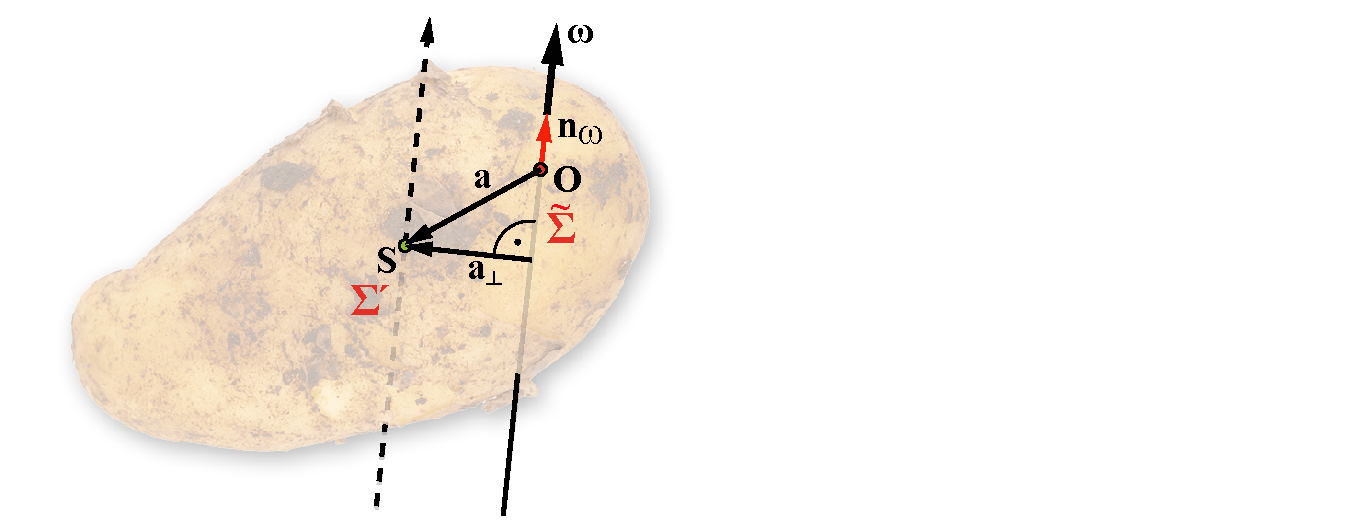
\includegraphics[width=\textwidth]{SteinerSatz.pdf}
  \caption[Steinerscher Satz.]{Steinerscher Satz. Die Rotation erfolge nun um eine Achse, die nicht durch den Schwerpunkt geht.
    Das neue Koordinatensystem $\tilde{\vec{\Sigma}}$ ist \emph{achsenparallel} zum k�rperfesten System (mit Ursprung im Schwerpunkt) $\vec{\Sigma}'$, allerdings mit seinem Ursprung nun auf der Drehachse.}
    \label{abb:bew_Steinerscher_Satz}
\end{figure}

Den Tr�gheitstensor hatten wir als Eigenschaft des K�rpers f�r die Berechnung
der kinetischen Energie \bzw des Drehimpulses eingef�hrt.
Wir wiederholen die Rechnung in dem neuen KOS $\tilde{\vec{\Sigma}}$ und k�nnen so erkennen, welchen Tr�gheitstensor wir f�r die neue Drehachse ben�tigen.%
\footnote{Wir erinnern daran, dass die kinetische Energie vom Bezugssystem abh�ngt
(\kap{bew_basics_of_systems}).}
Aus der kinetischen Energie \eqref{eq:bew_Kin_Energie_starrerK} wird jetzt
\begin{align}
  T  = T_\mathrm{trans} + T_\mathrm{rot}
  = T_\mathrm{trans} + \frac{1}{2} \int_V \tilde{\varrho}(\vec{\tilde{x}})\,
  (\vec{\omega} \times \vec{\tilde{x}})^2 \, \D^3 \tilde{x} ~ ,
\end{align}
wobei $T_\mathrm{trans}$ jetzt der Translation des Ursprungs von $\vec{\Sigma}'$
entspricht. 
F�hren wir die identische Rechnung zur Einf�hrung des Tr�gheitstensors ein zweites Mal aus, so sehen wir, dass sich der Tr�gheitstensor ergibt zu
\begin{align*}
  \tilde{\Theta}_{ij}
  &= \int_V \tilde{\varrho}(\vec{\tilde{x}}) \left (\vec{\tilde{x}}^2
    \delta_{ij} -\tilde{x}_i \tilde{x}_j \right ) \,\D^3 \tilde{x} \\
  &= \int_V \varrho(\vec{x}) \left ( (\vec{a} + \vec{x})^2 \delta_{ij} -
    (a_i+x_i) (a_j+x_j)  \right ) \,\D^3 x~.
\end{align*}
Ber�cksichtigt man erneut, dass Terme der Form $\varrho(\vec{x})x_i$
verschwinden, erh�lt man
\begin{align}
  \tilde{\Theta}_{ij}
  &= \int_v \varrho(\vec{x})\left ( \vec{x}^2 \delta_{ij} - x_i x_j \right )
  \,\D^3 x
  + \int_v \varrho(\vec{x}) \left ( \vec{a}^2 \delta_{ij} - a_i a_j \right )
  \,\D^3 x \notag \\
  &= \Theta_{ij} + M \left ( \vec{a}^2 \delta_{ij} - a_i a_j \right )\,.
\end{align}
Dies ist der \emph{Steinersche}%
\footnote{Jakob Steiner (1796--1863) war ein Schweizer Mathematiker,
der vor allem auf dem Gebiet der sogenannten synthetischen Geometrie arbeitete.}
Satz\index{Steinersche Satz}\indexp{Steiner, Jakob}:
Der Tr�gheitstensor (\bzw das Tr�gheitsmoment) f�r eine Rotation, die
nicht um den Schwerpunkt erfolgt, ist gleich der Summe aus dem Tr�gheitstensor
$\Theta$ f�r die Rotation um den Schwerpunkt und einem zweiten Anteil, der
so gro� ist, als w�rde die gesamte Masse des K�rpers im Schwerpunkt vereint um die neue Drehachse rotieren.\\
Daraus folgt insbesondere, dass das Tr�gheitsmoment f�r eine Rotation um den Schwerpunkt immer kleiner ist als das f�r jede dazu parallel verschobene Drehachse.
Diese Beziehungen gelten nat�rlich genauso f�r das Tr�gheitsmoment bez�glich einer festen Achse. Mit der Aufteilung
\begin{equation*}
  \omega^2 \left ( \vec{n_\omega} \times \vec{\tilde{x}} \right )^2 =
  \omega^2 \left ( \vec{n_\omega} \times \left ( \vec{a} + \vec{x} \right )
  \right )^2 =  \omega^2 \left ( {a_\perp}^2 + 2 \left (  \vec{n_\omega} \times
      \vec{a} \right ) \cdot \left (  \vec{n_\omega} \times \vec{x} \right )
    + {x_\perp}^2 \right )
\end{equation*}
in der kinetischen Energie erh�lt man (wobei lineare Terme in $\vec{x}$ im Integral wieder verschwinden)
\begin{align*}
  T_\mathrm{rot}
  &= \frac{1}{2} \omega^2 \int_V \varrho(\vec{x})\,{x_\perp}^2
    \,\D^3 x +  \frac{1}{2} \omega^2 \int_V \varrho(\vec{x})\, {a_\perp}^2 \,\D^3 x \\
  &= \frac{1}{2} \omega^2 \int_V \varrho(\vec{x}) \,{x_\perp}^2
    \,\D^3 x + \frac{1}{2} M \,{a_\perp}^2 \,\omega^2 
\end{align*}
oder das Tr�gheitsmoment
\begin{equation}
  \tilde{J} = J + M {a_\perp}^2 ~ , \label{eq:bew_SteinerSatz}
\end{equation}
also ebenfalls die Summe aus dem urspr�nglichen Tr�gheitsmoment und einem weiteren Term, der der Rotation der im Schwerpunkt vereinten Gesamtmasse senkrecht zur Drehachse entspricht.\\
Der Steinersche Satz erlaubt eine sehr simple Berechnung von Tr�gheitsmomenten f�r K�rper, die aus einfachen K�rperformen zusammengesetzt sind, da die Definition des Tr�gheitstensors \eqref{eq:bew_traegheitstensor} additiv ist (\probref{bew_traegheitsmomente}). 
Der Tr�gheitstensor eines starren K�rpers ist also die Summe der Tr�gheitstensoren seiner Teile (bei gleichem Bezugspunkt).
Dabei wird als Bezugspunkt f�r einen frei beweglichen starren K�rper am besten der Schwerpunkt gew�hlt, bei K�rpern, die in einem Punkt \bzw in einer Achse ortsfest sind, ist dieser Punkt \bzw diese Achse der Bezugspunkt/die Bezugsachse und das Tr�gheitsmoment wird �ber den Steinerschen Satz berechnet.

\subsection{Bewegungsgleichung des starren K�rpers}\label{kap:bew_BWG_StarrerK}

F�r die Bewegungsgleichungen eines starren K�rpers l�sst sich ausnutzen, dass wir bereits Ausdr�cke f�r den Gesamtimpuls und den Gesamtdrehimpuls gefunden haben.
Die Schwerpunktsbewegung wird durch die Summe der an den K�rper angreifenden Kr�fte bestimmt:
\begin{equation}
  \frac{\D \vec{P}_S}{\D t} =  \int_V \vec{f}(\vec{x})\, \D^3 x = \vec{F}\,.
\end{equation}
Die zeitliche �nderung des Gesamtdrehimpulses ergibt sich durch das
von au�en angreifende Drehmoment nach Gleichung
\eqref{eq:bew_Drehmoment_starrer_K}:
\begin{equation}
  \frac{\D\, \vec{L}}{\D t} = \vec{M}_\text{D}\,. \label{eq:bew_DrehimpulsSatz}
\end{equation}
Wir interessieren uns im Normalfall jedoch speziell f�r die Drehbewegung
des starren K�rpers unabh�ngig von der Bewegung des Schwerpunkts.
Gehen wir zus�tzlich noch davon aus, dass die Drehbewegung um den Schwerpunkt erfolgt \bzw die Drehachse durch den Schwerpunkt geht, beschreiben wir die Drehbewegung am besten im Schwerpunktsystem.
In diesem gilt $\vec{R}_S = \vec{0}$.
Damit verschwindet der Schwerpunktdrehimpuls $\vec{L}_S$ in Gleichung
\eqref{eq:bew_Gesamtdrehimpuls_starrer_K}.
Das Drehmoment aus
\eqref{eq:bew_Drehmoment_starrer_K} reduziert sich zu
\begin{equation*}
  \vec{M}_\text{D} = \int_V \left ( \vec{x} \times \vec{f}(\vec{x}) \right )\, \D^3 x
\end{equation*}
und man erh�lt
\begin{equation}
  \frac{\D\, \vec{L}_\mathrm{rot}}{\D t} = \frac{\D}{\D t} \underline{\vec{\Theta}} \,\vec{\omega}
  = \vec{M}_\text{D} = \int_V \left ( \vec{x} \times \vec{f}(\vec{x}) \right )\, \D^3 x
  ~ .
  \label{eq:bew_Drehbew_starrer_K}
\end{equation}
Die �nderung des Drehimpulses ist also gleich dem gesamten von au�en angreifenden Drehmoment.
Auch dieses Ergebnis hatten wir f�r starre Massepunktsysteme in \kap{bew_basics_of_systems} bereits hergeleitet.

\subsubsection{Euler-Gleichungen} \index{Euler-Gleichung}\label{kap:bew_Euler_Gl}

Die Bewegungsgleichung \eqref{eq:bew_Drehbew_starrer_K} f�r die Drehbewegung ist im raumfesten System mit zeitabh�ngigem Tr�gheitstensor $\Theta(t)$ gegeben. 
Vorteilhafter ist allerdings die Darstellung in einem k�rperfesten System, da dort $\underline{\vec{\Theta}}$ konstant ist.
Deswegen wollen wir nun die Bewegungsgleichung %mit der Drehmatrix $\mathbb{R}$
in ein k�rperfestes System $\vec{\Sigma}'$ transformieren.
Wir erhalten
\begin{subequations}
  \begin{align}
    \frac{\D}{\D t} \vec{L'}_\mathrm{rot} + \vec{\omega}' \times
    \vec{L}_\mathrm{rot}' = \vec{M}_\text{D}'
    \intertext{und da der Tr�gheitstensor im
    k�rperfesten System zeitlich konstant ist}
    \underline{\vec{\Theta}}' \dot{\vec{\omega}}' + \vec{\omega}' \times
    \underline{\vec{\Theta}}' \vec{\omega}'= \vec{M}_\text{D}' ~ .  \label{eq:bew_EulerGleichung01}
  \end{align}
\end{subequations}
Man beachte, dass selbst bei $\vec{M}_\text{D}'=\vec{0}$ der Drehimpuls nicht erhalten ist, da das System $\vec{\Sigma}'$ kein Inertialsystem ist.
Gleichung \eqref{eq:bew_EulerGleichung01} besagt, dass die zeitliche �nderung des Drehimpulses und das Drehmoment beim starren K�rper \ia nicht parallel sind.
Die Gleichungen sind nichtlinear in $\vec{\omega}'$ und deswegen relativ kompliziert zu l�sen.

Wir betrachten im Folgenden die Bewegung zun�chst nur in einem k�rperfesten System, welches als Haupttr�gheitsachsensystem gew�hlt ist. Dann k�nnen wir
die Komponentengleichungen von \eqref{eq:bew_EulerGleichung01} wie folgt schreiben:
\begin{equation}
  \begin{aligned}
    \Theta_{11} \, \dot{\omega}'_1 + (\Theta_{33}-\Theta_{22}) \,\omega'_2 \,\omega'_3 &= J_1 \, \dot{\omega}'_1 + (J_3-J_2) \,\omega'_2 \,\omega'_3 = M'_1\; ,\\
    \Theta_{22} \, \dot{\omega}'_2 + (\Theta_{11}-\Theta_{33}) \,\omega'_1 \,\omega'_3 &= J_2 \, \dot{\omega}'_1 + (J_1-J_3) \,\omega'_1 \,\omega'_3 = M'_2\; ,\\
    \Theta_{33} \, \dot{\omega}'_3 + (\Theta_{22}-\Theta_{11}) \,\omega'_1 \,\omega'_2 &= J_3 \, \dot{\omega}'_1 + (J_3-J_2) \,\omega'_1 \,\omega'_2 = M'_3 \;.
		\label{eq:bew_EulerGleichung02} 
  \end{aligned}
\end{equation}
Gleichungen \eqref{eq:bew_EulerGleichung01} und \eqref{eq:bew_EulerGleichung02} sind die \emph{Euler-Gleichungen} \index{Euler-Gleichung|textbf} f�r die Rotation eines starren K�rpers. 
Sie entsprechen den Newtonschen Bewegungsgleichungen f�r Massepunkte.
Der Einfachheit halber werden in der Literatur h�ufig die Striche f�r die Gr��en $\vec{M'}_\text{D}$ und $\vec{\omega}'$ des k�rperfesten Systems $\vec{\Sigma}'$ bei den Variablen weggelassen, wenn klar ist, dass man in $\vec{\Sigma}'$ rechnet.
Aber auch in diesen F�llen m�ssen wir uns immer in Erinnerung halten, dass die Gr��en in den Bewegungsgleichungen (Euler-Gleichungen) in Koordinaten des k�rperfesten Systems aufgeschrieben sind. 

\subsubsection{Euler-Winkel}\index{Euler-Winkel} \label{kap:bew_EulerWinkel}

Wir haben bei der Herleitung der Euler-Gleichungen angenommen, dass wir die momentane Winkelgeschwindigkeit in Koordinaten des k�rperfesten Systems $\vec{\Sigma}'$ ausdr�cken k�nnen. 
Das ergibt die einfache Struktur von \eqref{eq:bew_EulerGleichung02}, macht aber den Vektor $\vec{\omega}'$ sehr unanschaulich. 
Eleganter w�re eigentlich, die Bewegung im raumfesten System $\vec{\Sigma}$ zu beschreiben. 
Dazu f�hren wir drei zeitabh�ngige Winkel, die sogenannten \emph{Euler-Winkel} oder auch \emph{Eulerschen Winkel}\index{Euler-Winkel}\index{Eulersche Winkel} ein. 
Diese geben die momentane Orientierung des k�rperfesten Systems $\vec{\Sigma}'$ und damit des K�rpers im raumfesten System $\vec{\Sigma}$ an.

Wir nehmen an, dass $\vec{\Sigma}'$ und $\vec{\Sigma}$ einen gemeinsamen Ursprung haben. 
Durch eine zeitabh�ngige Rotation, welche eine Summe dreier Einzeldrehungen ist, kann man $\vec{\Sigma}$ in $\vec{\Sigma}'$ transformieren. 
Diese drei Winkel, die ben�tigt werden, um die Rotation vollst�ndig zu beschreiben, sind gerade die Euler-Winkel. 
Die Einzeldrehungen, f�r die das raumfeste System $\vec{\Sigma}$ (Achsen $\veceX$, $\veceY$, $\veceZ$) aus dem k�rperfesten $\vec{\Sigma}'$ (Achsen $\vecpeX$, $\vecpeY$, $\vecpeZ$) hervorgeht, sind:
\begin{enumerate}
\item Drehung um die Achse $\veceZ$ um den Winkel $\varphi$.
  (Die neue tempor�re $\veceX$-Achse hei�t Knotenlinie.)
\item Drehung um die Knotenlinie um den Winkel $\vartheta$.
\item Drehung um die nun erhaltene $\vecpeZ$-Achse um den Winkel $\psi$.
\end{enumerate}
Alle Drehungen erfolgen dabei in mathematisch positiver Richtung. Um letztlich die Bewegung des starren K�rpers im System $\vec{\Sigma}$ beschreiben zu k�nnen, m�ssen wir die Beziehung zwischen $\vec{\omega}$ und den Euler-Winkeln ermitteln.
Dazu betrachtet man eine kleine Drehung  $\vec{\omega}\,\D t$, die sich aus jeweils infinitesimalen �nderungen der Euler-Winkel um $\D \varphi$ um die Achse $\veceZ$, um $\D \vartheta$ um die Knotenlinie und um $\D \psi$ um die $\vecpeZ$-Achse zusammensetzt. 
Diese infinitesimale Drehung kann man aus geometrischen �berlegungen aus \figref{bew_EulerWinkel} ableiten und benutzt dabei die Rotationsmatrizen aus \kapitel{bew_rotating_systems}. 
Wir m�chten dies hier nicht im Einzelnen tun, sondern verweisen stattdessen auf \probref{bew_EulerWinkel} und geben hier lediglich das Ergebnis an:
\begin{align}
\vec{\omega}' = 
\begin{pmatrix}	\omega'_1 \\ \omega'_2 \\ \omega'_3 \end{pmatrix} = \,
\begin{pmatrix}
		\dot{\varphi}\,\sin\vartheta\,\sin\psi + \dot{\vartheta}\,\cos\psi \\
		\dot{\varphi}\,\sin\vartheta\,\cos\psi - \dot{\vartheta}\,\sin\psi \\
		\dot{\varphi}\,\cos\vartheta + \dot{\psi}
\end{pmatrix}. \label{eq:bew_EulerWinkel} 
\end{align}
\begin{figure}
  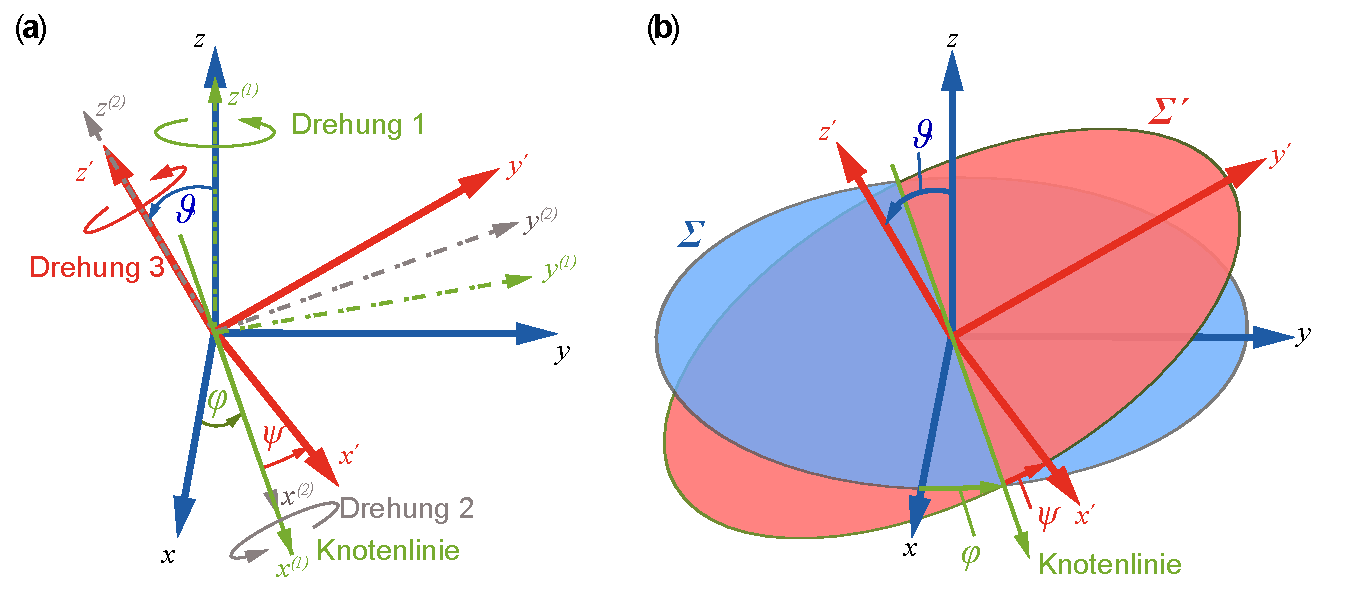
\includegraphics[width=0.95\textwidth]{EulerWinkel.pdf}
    \caption[Definition der Euler-Winkel.]{%
    \fa Definition der Euler-Winkel als Verkn�pfung dreier
    Rotationen. \fb
    Perspektivische Darstellung der Koordinatensysteme
    $\vec{\Sigma}$ und $\vec{\Sigma}'$ mit den Euler-Winkeln.}\label{abb:bew_EulerWinkel}
\end{figure}
Sind die Parameter f�r die Dynamik eines starren K�rpers durch $\vec{J}$ und $\vec{M}'$ gegeben, muss man also zun�chst aus den Euler-Gleichungen \eqref{eq:bew_EulerGleichung02} die momentane Winkelgeschwindigkeit $\vec{\omega}'(t)$ (in Koordinaten von $\vec{\Sigma}'$) bestimmen. 
Damit kann man dann die drei gekoppelten Diffentialgleichungen \eqref{eq:bew_EulerWinkel} nach $\varphi(t),\,\vartheta(t),\,\psi(t)$ l�sen. 
Das wird recht schwierig, denn einerseits ist \eqref{eq:bew_EulerGleichung02} eine nichtlineare DGL, andererseits liegen die gesuchten Gr��en (Euler-Winkel) in \eqref{eq:bew_EulerWinkel} auch noch als Argumente von Winkelfunktionen vor. Wir werden dennoch eine L�sung versuchen und uns dem allgemeinen Problem zun�chst �ber ein paar Spezialf�lle n�hern. Wir werden den Euler-Winkeln �brigens in der Himmelsmechanik (Band II, Kapitel 3) in etwas anderer Notation wieder begegnen.

\subsection{Kreisel} \label{kap:bew_Kreisel}

\subsubsection{Rotation eines \emph{kr�ftefreien} Kreisels} \index{Kreisel}\index{Kreisel!kr�ftefreier|textbf}\label{kap:bew_kfKreisel}

Ein Kreisel ist ein starrer K�rper, der um eine Achse rotiert.
In einer ersten Einschr�nkung werden wir davon ausgehen, 
dass er um eine Achse durch seinen Schwerpunkt rotiert.
Auf diesen k�nnen also die Eulerschen Kreiselgleichungen
\eqref{eq:bew_EulerGleichung02} angewendet werden.
Zun�chst werden wir den
Spezialfall des kr�ftefreien Kreisels betrachten.
F�r diesen verschwindet
also das Drehmoment $\MD$ und die Euler-Gleichungen
\eqref{eq:bew_EulerGleichung02} lassen sich auf die Form
\begin{equation}
  \begin{aligned}
    J_1 \, \dot{\omega}_1' + (J_3-J_2) \,\omega_2' \,\omega_3' = 0\\
    J_2 \, \dot{\omega}_2' + (J_1-J_3) \,\omega_1' \,\omega_3' = 0\\
    J_3 \, \dot{\omega}_3' + (J_2-J_1) \,\omega_1' \,\omega_2' = 0
  \end{aligned}
  \label{eq:bew_Kreisel_frei}
\end{equation}
bringen.
Man realisiert einen kr�ftefreien Kreisel \zb dadurch, dass man ihn im Schwerpunkt $S$ unterst�tzt und 
damit die Schwerkraft kompensiert.
Alternativ betrachtet man einen frei fallenden Kreisel im bewegten Koordinatensystem.
Sch�ne und instruktive Experimente zum kr�ftefreien Kreisel sind auf der ISS von Alexander 
Gerst\footnote{Alexander Gerst (geb.~1976) ist ein deutscher Geophysiker, Vulkanologe und Astronaut.
Er flog zweimal zur Internationalen Raumstation ISS\index{ISS!Internationale Raumstation}\indexp{Gerst, Alexander} 
und �bernahm am 3.\,10.\,2018 f�r fast drei Monate als erster Deutscher
die Funktion des ISS-Kommandanten.} 
durchgef�hrt worden \cite{Gerst2018}.

Man sieht an \eqref{eq:bew_Kreisel_frei} sofort, dass sich aus \eqref{eq:bew_Kreisel_frei} f�r den Fall einer Rotation um eine der Haupttr�gheitsachsen 
(also um eine der Koordinatenachsen von $\vec{\Sigma}'$, \zb $\omega_1'=\omega_0'$ mit $\omega_2'=\omega_3'=0$) 
$\dot{\vec{\omega}'}=\vec{0}$
ergibt und die Rotation somit zeitlich konstant ist. 

Dies gilt jedoch nur f�r eine exakte Ausrichtung entlang einer der
Haupttr�gheitsachsen, was sich in der Realit�t nicht erf�llen lassen wird.
Um die Stabilit�t solcher Drehungen nahe einer der Haupttr�gheitsachsen zu untersuchen, 
legen wir das Koordinatensystem so, dass $J_1 > J_2 > J_3$ gilt. 
Weiterhin nehmen wir an, dass wir eine kleine St�rung $\vec{\Delta\omega}'$ der Rotation um eine der Haupttr�gheitsachsen haben.
Setzt man \zb f�r eine Rotation um die $\vecpeX$-Achse einen \anf{gest�rten} Vektor der Winkelgeschwindigkeit 
\begin{equation}
  \vec{\omega}_0' + \vec{\Delta\omega}' = 
  \begin{pmatrix} \omega_0'
    + \Delta\omega_1'(t) \\  \Delta\omega_2'(t) \\ \Delta\omega_3'(t)
  \end{pmatrix} \label{eq:bew_Kreisel_frei_lin}
\end{equation}
an und linearisiert die Bewegungsgleichungen in den $\Delta\omega_i'$, so
findet man als Ergebnis, dass die St�rung in der
$\vecpeY$-$\vecpeZ$-Ebene erhalten bleibt, jedoch nicht gr��er wird.
Eine
Rotation um die $\vecpeX$-Achse ist also stabil.
Gleiches findet man f�r
eine Rotation um die $\vecpeZ$-Achse.
Jedoch wird, falls eine Rotation
um die $\vecpeY$-Achse gest�rt wird, die St�rung exponentiell anwachsen.
Eine solche Rotation ist also instabil.
Die ausf�hrliche Betrachtung erfolgt
numerisch in  Beispiel \ref{bsp:bew_unsymm_Kreisel} und \probref{bew_freier_Kreisel}. 
Wir merken uns jedoch, dass f�r einen nicht-symmetrischen
Kreisel die Rotationen nur um die beiden Haupttr�gheitsachsen mit dem jeweils gr��ten bzw. kleinsten
Tr�gheitsmoment stabil sind.
Eine Rotation um die Haupttr�gheitsachse mit dem
mittleren Tr�gheitsmoment ist instabil.

%BEISPIEL %%%%%%%%%%%%%%%%%%%%%%%%%%%%%%%%%%%%%%%%%%%%%%%%%%%%%%%%%%%%%%%%%%%%%%%%%%%%%%%%%%
\begin{example}{St�rung der Rotation um freie Haupttr�gheitsachsen }
\label{bsp:bew_unsymm_Kreisel}
\medskip

Die Bewegungsgleichungen \eqref{eq:bew_Kreisel_frei} des kr�ftefreien unsymmetrischen
Kreisels lassen sich numerisch einfach integrieren.
Damit l�sst sich die
Stabilit�t der Rotationen um die Haupttr�gheitsachsen gut analysieren.
Wir
w�hlen das Verh�ltnis der drei Haupttr�gheitsmomente $J_1 : J_2 : J_3 =
3:4:5$, $J_1$ und $J_2$ sind also die extremen Tr�gheitsmomente und $J_2$
liegt dazwischen.
Die N�herung f�r kleine St�rungen (siehe \probref{bew_freier_Kreisel}) sagt voraus, dass die
Rotationen um die $\vecpeX$- und $\vecpeZ$-Achsen stabil, die um
$\vecpeY$ instabil sein sollten.
Die exemplarischen Ergebnisse sind (numerisch im \mscr{} 
\mlbewref{KfKreiselFreieAchsen.m} ausgef�hrt) wie folgt:

\begin{itemize}
\item F�r eine Rotation um die $\vecpeX$-Achse mit
  $\omega_1' = 1/\mathrm{s}$, die leicht durch einen zus�tzlichen Beitrag
	$\Delta \omega_2'$ gest�rt wird, ergibt sich Bild \figref{bew_KfKreiselstabil}.
 
\begin{center}
    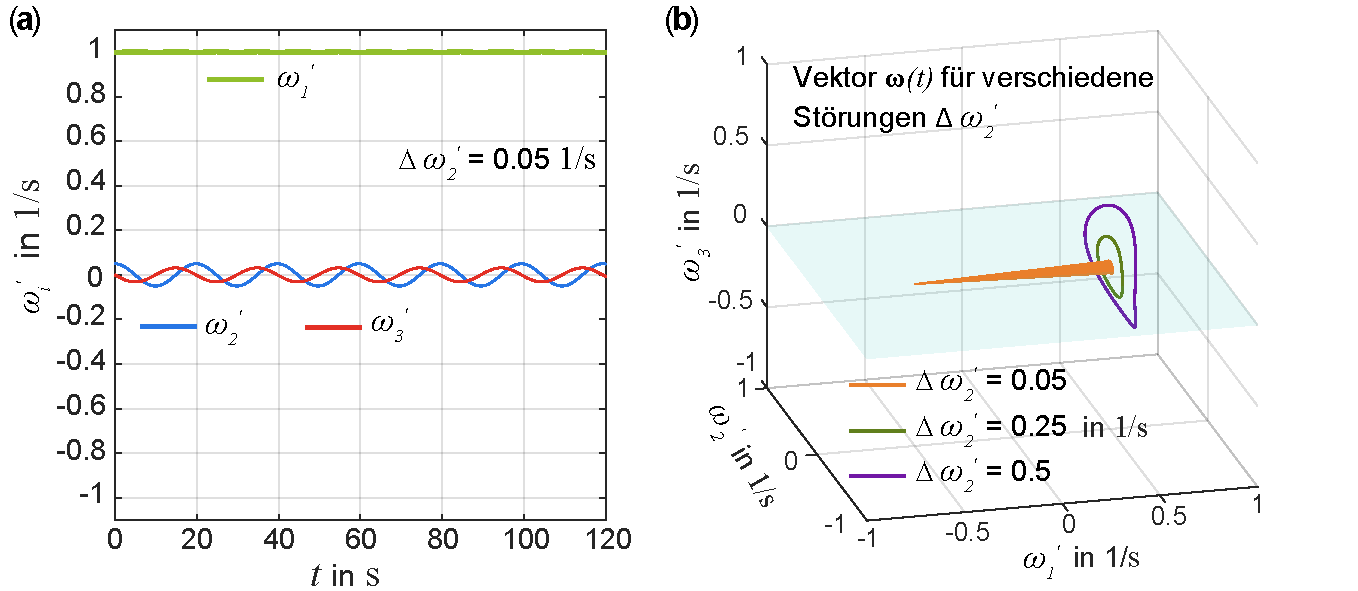
\includegraphics[width=\textwidth]{KfKreiselstabil.pdf}
\captionof{figure}{Stabile Rotation eines kr�ftefreien Kreisels um seine Hauptachsen.}\label {abb:bew_KfKreiselstabil}
\end{center}

Im linken Teil von \figref{bew_KfKreiselstabil} sieht man den zeitlichen
Verlauf der drei Kreisfrequenzen f�r eine Anfangsst�rung von
$\Delta \omega_2'= \SI{0.05}{\per\s}$.
Die Erwartung aus der linearen N�herung der St�rung \eqref{eq:bew_Kreisel_frei_lin}
ist gut erf�llt. Es ergibt sich eine Oszillation der St�rung zwischen der
$\vecpeY$- und $\vecpeZ$-Richtung, sie wird jedoch betragsm��ig nicht gr��er.
Die Rotation um die $\vecpeX$-Achse �ndert sich kaum. Dies erkennt man auch
in der rechten Abbildung, in der der zeitliche Verlauf aller drei Komponenten
von $\vec{\omega}'$ dargestellt ist.
F�r die kleinen Anfangsst�rungen $\Delta \omega_2' = \SI{0.05}{\per\s}$ und
$\Delta\omega_3' = \SI{0.05}{\per\s}$ oszilliert die Spitze des Vektors
$\vec{\omega}'$ mit kleinen Abst�nden um den eigentlich beabsichtigten Wert
$\vec{\omega}' = (1.0,0,0)\SI{}{\per\s}$ (linkes Bild).
Erst f�r die deutlich gr��ere St�rung von $\Delta \omega_2' \geq \SI{0.25}
{\per\s}$ ergibt sich eine leichte sichtbare Abweichung der Richtung des
Vektors $\vec{\omega}'$ und auch eine zeitliche Variation von $\omega_1'(t)$.

\item Nun betrachten wir eine Rotation um die $\vecpeY$-Achse (mit dem mittleren Tr�gheitsmoment $J_2$ 
und der Winkelgeschwindigkeit $\omega_2' = \SI{1.0}{\per\s}$), die 
wiederum durch einen kleinen zus�tzlichen Beitrag, hier nun $\Delta \omega_1'$, gest�rt wird.
Die Erwartung aus der linearen N�herung mit dem Ansatz
\eqref{eq:bew_Kreisel_frei_lin} ist nun, dass sich die St�rung exponentiell
vergr��ert.  Dies geschieht auch f�r die Anfangsst�rung
$\Delta \omega_1' = \SI{0.05}{\per\s}$ zun�chst.
Dann wird die St�rung jedoch so
gro�, dass die lineare N�herung nicht mehr g�ltig ist.
Es ergibt sich eine in (\figref{bew_KfKreiselinstabil}) deutlich sichtbare
erhebliche Abweichung von der urspr�nglichen Rotation, bei der im Zeitverlauf
alle drei Komponenten von $\vec{\omega}'$ �hnlich gro�e Werte annehmen und die
Bewegung nichts mehr mit einer reinen Rotation um die $\vecpeY$-Achse
zu tun hat.
Obwohl die St�rung am Beginn nicht gr��er ist als im vorherigen
Beispiel, ergibt sich nach kurzer Zeit ein vollst�ndig anderes Verhalten.
Durch die Instabilit�t der Achse spielt es fast keine Rolle, wie gro�
die Anfangsst�rungen sind, wie man im rechten Teil von
\figref{bew_KfKreiselinstabil} erkennt. F�r die Anfangsst�rungen
$\Delta \omega_1' = \SI{0.05}{\per\s}$, $\SI{0.25}{\per\s}$ und
$\SI{0.5}{\per\s}$ ergibt sich jeweils ein sehr �hnliches Verhalten. 

\begin{center}
    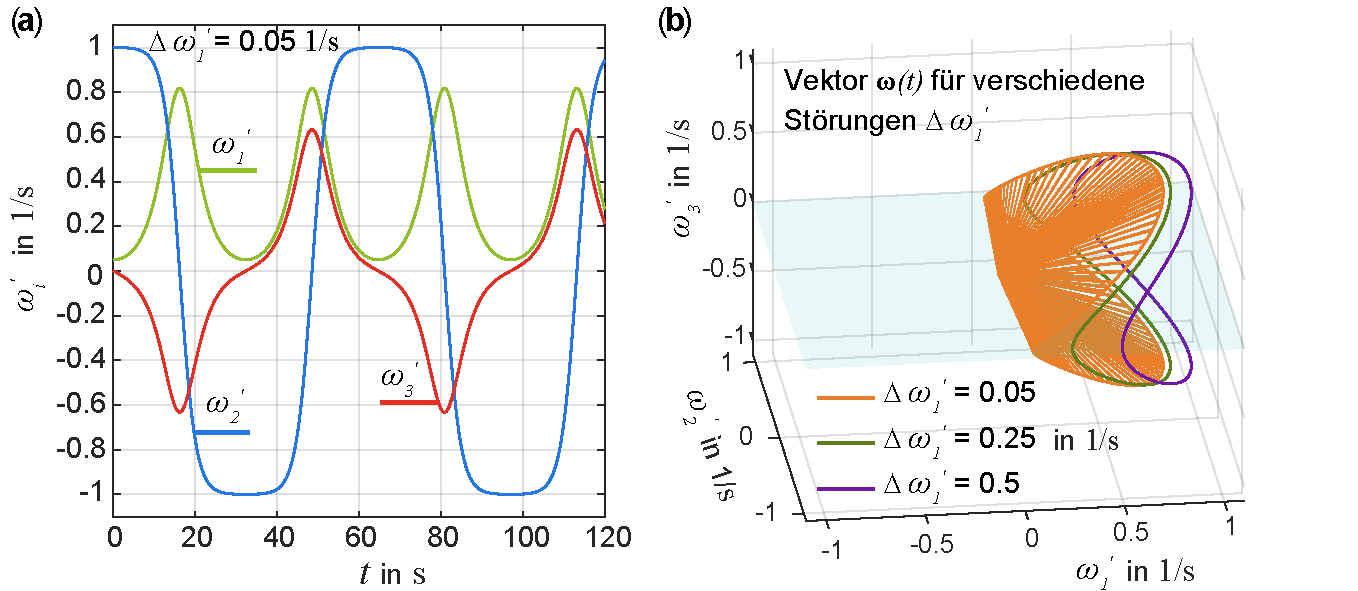
\includegraphics[width=\textwidth]{KfKreiselinstabil.pdf}
\captionof{figure}{Instabile Rotation eines kr�ftefreien Kreisels um seine freien Hauptachsen.}\label {abb:bew_KfKreiselinstabil}
\end{center}

\end{itemize}
\end{example}
%BEISPIEL %%%%%%%%%%%%%%%%%%%%%%%%%%%%%%%%%%%%%%%%%%%%%%%%%%%%%%%%%%%%%%%%%%%%%%%%%%%%%%%%%%

\subsubsection{Rotation eines kr�ftefreien \emph{symmetrischen} Kreisels} \index{Kreisel!kr�ftefreier!}\index{Kreisel!symmetrischer}\label{kap:bew_Kreisel_kraeftefrei}

Bisher haben wir nur freie Rotationen um die Haupttr�gheitsachsen des Kreisels betrachtet.
Wir wollen jetzt die Bewegung des Kreisels einschr�nken und den Kreisel \emph{im Schwerpunkt} festhalten \bzw unterst�tzen. Dieser Kreisel ist dann auch kr�ftefrei.
Eine solche Kr�ftefreiheit kann man dadurch realisieren, dass man den Kreisel in einer sogenannten kardanischen\footnote{Gerolamo Cardano\indexp{Cardano, Gerolamo} (1501--1576) war ein italienischer Arzt, Philosoph und Mathematiker. Er arbeitete auf vielen Gebieten, \ua in der Wahrscheinlichkeitsrechnung und Kombinatorik, in der Erforschung von Krankheiten wie Tuberkulose und Typhus und an mechanischen Konstruktionen. Nach ihm ist die kardanische Aufh�ngung und die Kardanwelle benannt.} (oder cardanischen)\index{Kardanische Aufh�ngung}\index{Cardanische Aufh�ngung} Aufh�ngung befestigt (Abb. \figref{bew_KfSymmKrRealisierung}). Alternativ kann man sich nat�rlich auch f�r entsprechende Studien an kr�ftefreien Kreiseln auf einen Raumflug begeben.\\
Als weiteren Spezialfall wollen wir den kr�ftefreien Kreisel als symmetrisch annehmen. 
Darunter versteht man
einen Kreisel, f�r den zwei Tr�gheitsmomente identisch sind, $J_1 = J_2
= J_{12} \neq J_3$. Die Achse $\vecpeZ$, die senkrecht zur den beiden
identischen Haupttr�gheitsmomenten steht, hei�t Figurenachse $\vec{f}$. 

\begin{figure}
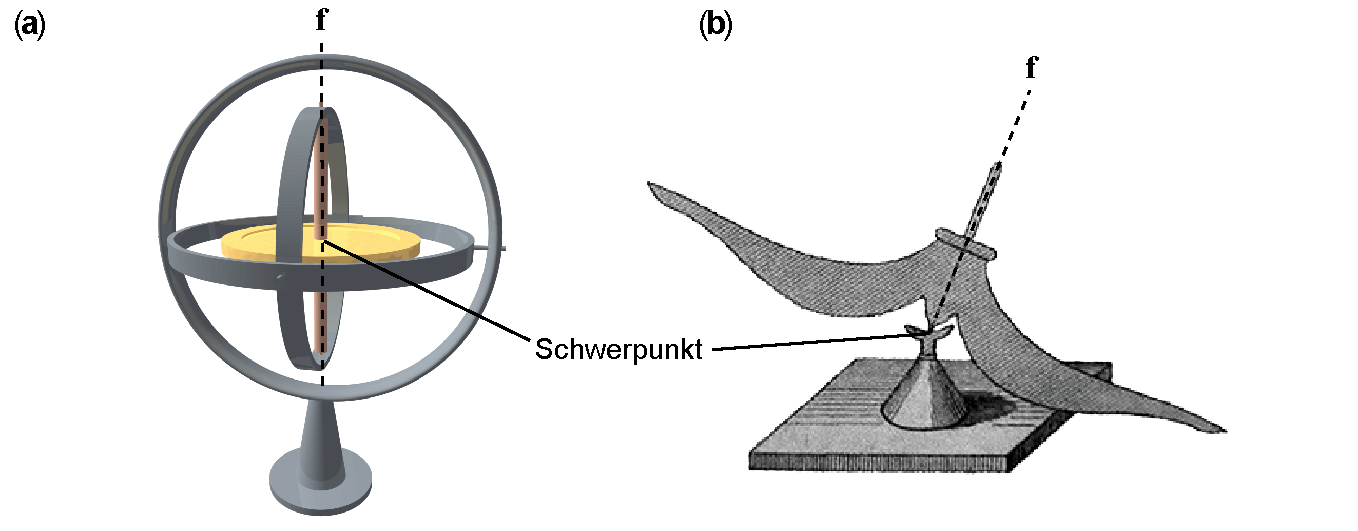
\includegraphics[width=\textwidth]{KfSymmKrRealisierung.pdf} 
	\caption[Realisierung des kr�ftefreien symmetrischen Kreisels.]{Realisierung des kr�ftefreien symmetrischen Kreisels \fa Kardanische Aufh�ngung (Euler-Kreisel) und \fb Unterst�tzung im Schwerpunkt (nach Klein\footnotemark\indexp{Klein, Felix Christian} und Sommerfeld \cite{Klein1910}).} \label{abb:bew_KfSymmKrRealisierung}
\end{figure}
\footnotetext{Felix Christian Klein (1849--1925) war ein deutscher Mathematiker, der im 19.~Jahrhundert bedeutende Fortschritte vor allem in der Geometrie erzielte. Klein besch�ftigte sich mit der Funktionentheorie und k�mmerte sich um die Anwendung der Mathematik. Er engagierte sich sehr f�r die Mathematikdidaktik und die Lehre generell. Sommerfeld war einer seiner besten Sch�ler.}

Da wir in diesem Kapitel den Kreisel sowohl im System $\vec{\Sigma}$ als auch im mitbewegten System $\vec{\Sigma'}$ betrachten wollen, kennzeichnen wir wie vereinbart die Gr��en im mitrotierenden System mit Strichen.
Aus den Kreiselgleichungen \eqref{eq:bew_EulerGleichung02} folgt damit
\begin{equation*}
  J_3\,\dot{\omega}_3' = 0 \qquad \text{und} \qquad \omega_3' = \con~ .
\end{equation*}
Setzt man mit dem Wissen, dass $\omega_3'$ konstant ist,
\begin{equation*}
  \Omega = \frac{J_3-J_{12}}{J_{12}} \,\omega_3' = \con~ ,
\end{equation*}
erh�lt man f�r die Bewegungsgleichungen der anderen beiden Komponenten
die gekoppelten Differentialgleichungen
\begin{equation*}
  \begin{aligned}
    \dot{\omega}_1' &= - \Omega \, \omega_2' ~ ,\\
    \dot{\omega}_2' &= \phantom{-}  \Omega \, \omega_1' ~ .\\
  \end{aligned}
\end{equation*}
Die L�sungen lassen sich einfach finden, da dieses DGL-System in eine DGL zweiter Ordnung �berf�hrt werden kann, 
die der harmonischen Schwingungsgleichung entspricht. Insgesamt erh�lt man
\begin{equation}
  \vec{\omega}' = 
	\begin{pmatrix} \omega_1' \\ \omega_2' \\ \omega_3' \end{pmatrix} = 
	\begin{pmatrix} \omega_\perp' \, \cos(\Omega \,t + \Delta
    \alpha) \\ \omega_\perp' \, \sin(\Omega\, t + \Delta \alpha) \\
    \omega_3' \end{pmatrix}
  \label{eq:bew_Nutation_omega}
\end{equation}
mit der zeitunabh�ngigen (konstanten) Amplitude
$\omega_\perp' = \sqrt{{\omega_1 '}^2 + {\omega_2 '^2}}$ der Drehung mit der betragsm��ig 
konstanten Winkelgeschwindigkeit
$\omega' = \left| \vec{\omega}'\right| = \sqrt{{\omega_\perp'}^2 + {\omega_3'}^2}$
um die $\vecpeZ$-Achse.
F�r den Drehimpuls gilt
\begin{equation}
  \vec{L}' = 
	\begin{pmatrix} J_{12}\,\omega_1' \\ J_{12}\,\omega_2' \\ J_3\, \omega_3' \end{pmatrix} =
	\begin{pmatrix} J_{12} \, \omega_\perp' \, \cos(\Omega\, t + \Delta
    \alpha) \\ J_{12} \, \omega_\perp' \, \sin(\Omega\, t + \Delta \alpha) \\
    J_3 \, \omega_3' \end{pmatrix} ~
  \label{eq:bew_Nutation_L}
\end{equation}

und damit $L'^2 = \con$, wie zu erwarten war.
Man sieht aus \eqref{eq:bew_Nutation_omega} und \eqref{eq:bew_Nutation_L}
also, dass sowohl $\vec{\omega}'$ als auch $\vec{L}'$ eine Drehung um
die $\vecpeZ$-Achse (die Figurenachse) des k�rperfesten Systems ausf�hren, allerdings in
unterschiedlicher Art und Weise, da nach \eqref{eq:bew_Nutation_L} $\vec{L}'$ und $\vec{\omega}'$ unterschiedliche
Richtungen haben (siehe \figref{bew_KfSymmKrNutation} a). Man nennt diese Bewegung \emph{Nutation} (aus dem Lateinischen \textit{nutare} f�r "`nicken"').\index{Nutation|textbf}\footnote{Vielfach wird diese Bewegung auch \textit{(regul�re) Pr�zession}\index{Pr�zession|textbf}\index{Pr�zession!regul�re|textbf} genannt, vor allem im angels�chsischen Raum. Auch Klein und Sommerfeld \cite{Klein1910} verwendeten diesen Begriff. Da wir den Begriff Pr�zession f�r eine Bewegung beim schweren Kreisel reservieren wollen, verwenden wir hier den Begriff Nutation.}

\begin{figure}
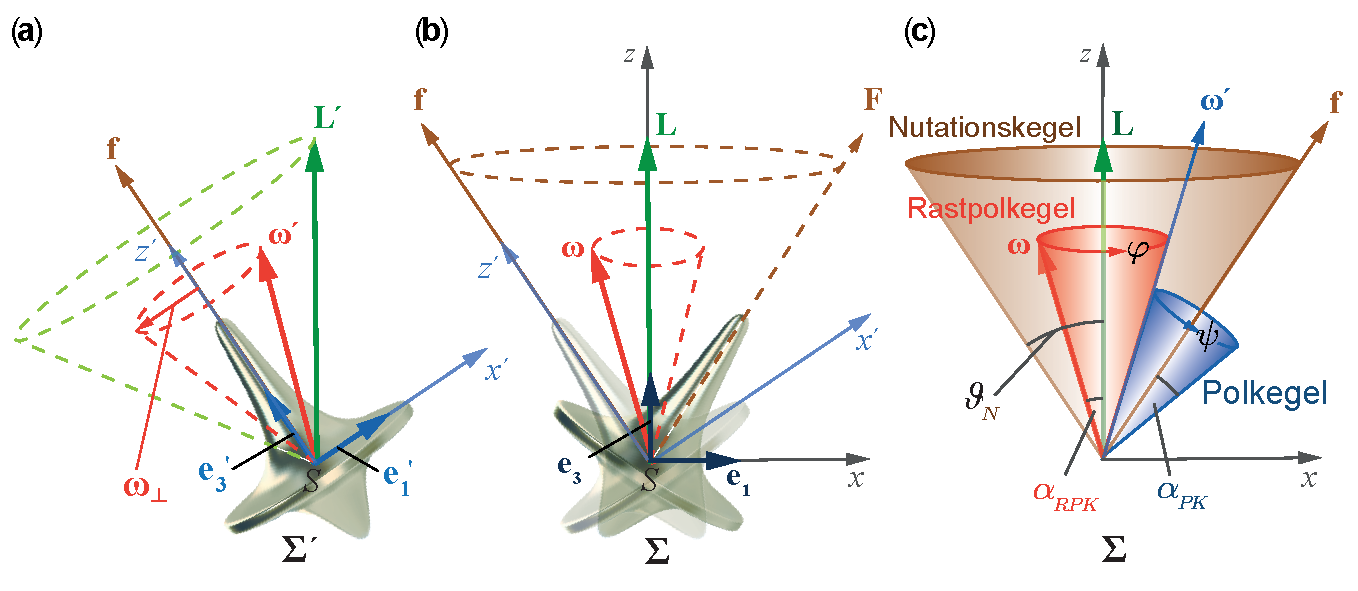
\includegraphics[width=\textwidth]{KfSymmKrNutation.pdf} 
	\caption[Nutation eines kr�ftefreien symmetrischen Kreisels.]{Ein kr�ftefreier symmetrischer Kreisel f�hrt eine Nutationsbewegung aus.
    \fa Im k�rperfesten System f�hren die Drehachse $\vec{\omega}'$ und auch der Drehimpuls $\vec{L}'$ eine Kreisbewegung um die Figurenachse $\vec{F}=\vecpeZ$
    aus. \fb Im raumfesten System ist der Drehimpuls f�r die kr�ftefreie Bewegung konstant. Man sieht eine Drehbewegung der Figurenachse und
    der momentanen Drehachse um die feststehende Drehimpulsachse. \fc �bersicht der Rotationsbewegungen der einzelnen Achsen des kr�ftefreien symmetrischen
Kreisels.
$\vartheta_\text{N}, \alpha_\text{PK}, \alpha_\text{RK}$ sind die �ffnungswinkel von Nutations-, Pol- \bzw Rastpolkegel.}\label{abb:bew_KfSymmKrNutation}
\end{figure}
Die Nutation ist zwar dynamisch, aber in ihrer periodischen Entwicklung stabil.
Wir nehmen diese jedoch f�r gew�hnlich nicht im k�rperfesten System wahr,
sondern beobachten sie aus dem raumfesten System heraus.
Da die Bewegung nach Voraussetzung kr�ftefrei ist und somit auch kein Drehmoment wirkt,
ist in diesem System der Drehimpuls nach Richtung und Betrag konstant,
die Drehimpulsachse liegt folglich stabil im Raum.
Die Figurenachse $\vec{f} = \vecpeZ$ rotiert auf dem \emph{Nutationskegel} mit dem 
�ffnungswinkel $\vartheta_\text{N}$ um die Drehimpulsachse. 
Wir wollen die Nutation im raumfesten System im folgenden Beispiel n�her untersuchen.
\newpage
%Begin BEISPIEL %%%%%%%%%%%%%%%%%%%%%%%%%%%%%%%%%%%%%%%%%%%%%%%%%%%%%%%%%%%%%%%%%%%%%%%%%%%%%%%%%%
\begin{example}{Dynamik der Nutation eines kr�ftefreien symmetrischen Kreisels}
  \medskip
	
	Es wurde bereits erw�hnt, dass die Nutationsbewegung dadurch gekennzeichnet ist, 
	dass die Drehimpulsachse fest im Raum steht,
  da aufgrund der Kr�fte- und Drehmomentfreiheit der Drehimpuls erhalten ist.
  Die Beschreibung der Drehbewegung im raumfesten System erfolgt mithilfe der Euler-Winkel
  \eqref{eq:bew_EulerWinkel}.
  Man erh�lt mit
  \eqref{eq:bew_Nutation_omega}
  \begin{equation}
    \begin{pmatrix} \omega_1'\\ \omega_2' \\ \omega_3' \end{pmatrix}
    = \begin{pmatrix} \omega_\perp' \, \cos(\Omega \,t + \Delta
      \alpha) \\ \omega_\perp' \, \sin(\Omega\,t + \Delta \alpha) \\
      \omega_3' \end{pmatrix}
    = \begin{pmatrix}
      \dot{\varphi}\,\sin\vartheta\,\sin\psi + \dot{\vartheta}\,\cos\psi \\
      \dot{\varphi}\,\sin\vartheta\,\cos\psi - \dot{\vartheta}\,\sin\psi \\
      \dot{\varphi}\,\cos\vartheta + \dot{\psi}
    \end{pmatrix} \; .
    \label{eq:bew_DGL_Eulerwinkel_Nutation}
  \end{equation}
  Das raumfeste System legen wir so, dass die Drehimpulsachse mit der
  $\veceZ$-Achse des KOS �bereinstimmt.
  Dann wird die Neigung der Figurenachse
  gegen�ber dem Drehimpuls gerade durch den Euler-Winkel $\vartheta$ ausgedr�ckt.
  Dieser berechnet sich nach nach \eqref{eq:bew_Nutation_L} zu
  \begin{equation}
    \vartheta_\text{N} = \arctan \lk \frac{\sqrt{{L_x'}^2 + {L_y'}^2}}{L_z'} \rk = \arctan \left ( \frac{J_{12} \omega_\perp'}{J_3 \omega_3'}
    \right ) \; . \label{eq:bew_Nutationswinkel}
  \end{equation}
  und ist, wie bereits erw�hnt, konstant.
  Gleichung \eqref{eq:bew_DGL_Eulerwinkel_Nutation} vereinfacht sich zu
  \begin{equation}
	   \begin{pmatrix} \omega_1'\\ \omega_2' \\ \omega_3' \end{pmatrix} =
		 \begin{pmatrix} \omega_\perp' \, \cos(\Omega\,t + \Delta
      \alpha) \\ \omega_\perp' \, \sin(\Omega\,t + \Delta \alpha) \\
      \omega_3' \end{pmatrix}
    = \begin{pmatrix}
      \dot{\varphi}\,\sin\vartheta_\text{N}\,\sin\psi \\
      \dot{\varphi}\,\sin\vartheta_\text{N}\,\cos\psi \\
      \dot{\varphi}\,\cos\vartheta_\text{N} + \dot{\psi}
    \end{pmatrix} \; .
    \label{eq:bew_DGLEuler_Nutation2}
  \end{equation}
  Eine L�sung findet man leicht, indem man die ersten beiden Zeilen dieser
  vektoriellen Gleichung quadriert und addiert.
  Daraus ergibt sich sofort
  \begin{equation}
    \dot{\varphi} = \frac{\omega_\perp'}{\sin\vartheta_\text{N}} = \Omega' \qquad
    \text{bzw.}\qquad \varphi(t) = \frac{\omega_\perp'}{\sin\vartheta_\text{N}}\,t  +\varphi_0 = \Omega' \,t +\varphi_0 \,. \label{eq:bew_DGLEuler_Nutation2a}
  \end{equation}
  Die dritten Zeile f�hrt mit diesem Resultat auf
  \begin{align*}
    \dot{\psi} &= \omega_3' - \omega_\perp' \cot\vartheta_\text{N} = \omega_3'
    - \frac{J_3\,\omega_3'}{J_{12}} = \frac{J_{12}-J_3}{J_{12}}\,\omega_3'
                 = \con = -\, \Omega \\
    \text{\bzw} \qquad \psi(t) &= -\, \Omega \, t + \psi_0 \; .
  \end{align*}
  Ein Vergleich mit den ersten beiden Zeilen legt die Integrationskonstante
  $\psi_0$ fest auf $\psi_0 = -\Delta \alpha \pm \pi/2$, sodass
  \begin{equation}
    \psi(t) = -\,\Omega\, t  - \Delta \alpha \pm \frac{\pi}{2} \; . \label{eq:bew_DGLEuler_Nutation2b}
  \end{equation}
  Damit haben wir in diesem geeignet gew�hlten Koordinatensystem $\vec{\Sigma}$ alle drei Euler-Winkel bestimmt.
  Die Figurenachse, die mit dem konstanten 
  Winkel $\vartheta_\text{N}$ gegen den konstanten Drehimpuls geneigt ist, l�uft mit der konstanten Winkelgeschwindigkeit $\dot{\varphi} = \Omega'$ um den raumfesten Drehimpuls herum.
	Dazu dreht sich der Kreisel mit der ebenfalls konstanten Winkelgeschwindigkeit $\dot{\psi} = \Omega$ um seine Figurenachse. 
	Dieses Ergebnis l�sst sich auch numerisch finden.
  Dazu bringt man die Gleichungen \eqref{eq:bew_DGLEuler_Nutation2} auf eine geeignete
  Form, in der die drei Zeitableitungen der Euler-Winkel isoliert auf den linken Seite des Gleichungssystems stehen.
	Dies gelingt \zb f�r $\dot{\varphi}$ durch
  die Multiplikation der ersten Zeile mit $\sin\psi$ und Addition der mit
  $\cos\psi$ multiplizierten zweiten Zeile.  Analog ergibt sich durch Multiplikation der ersten Zeile mit $\cos\psi$
  und Subtraktion der zweiten mit $\sin\psi$ multiplizierten Zeile eine
  Differentialgleichung f�r $\dot{\vartheta}$ und schlie�lich gewinnt man aus der dritten Zeile von \eqref{eq:bew_DGLEuler_Nutation2} 
	unter Nutzung der Beziehung f�r $\dot{\varphi}$ eine Beziehung f�r $\dot{\psi}$. Insgesamt erh�lt man also
\begin{align}
  \frac{\D}{\D t}\, {\begin{pmatrix}\varphi\\\vartheta\\\psi\end{pmatrix}}
    =
    \begin{pmatrix}
      \frac{\sin\psi}{\sin\vartheta} & \frac{\cos\psi}{\sin\vartheta} & 0 \\
      \cos\psi               & -\sin\psi              & 0 \\
      -\sin\psi\cot\vartheta         & -\cos\psi\cot\vartheta         & 1
    \end{pmatrix} \,
    \vec{\omega}\,.
  \label{eq:bew_DGLEuler_Nutation2c}
\end{align}
Integriert man diese gekoppelten Differentialgleichungen erster Ordnung mit den passenden Anfangsbedingungen $\vartheta(0) = \vartheta_\text{N}$,
$\psi(0) = -\Delta \alpha \pm \frac{\pi}{2}$ (und einem beliebigen $\varphi(0)$), so findet man die in \figref{bew_SymmKreiselEulerWinkel} 
dargestellte numerische L�sung f�r die Winkelgeschwindigkeit $\vec{\omega}$ und die Euler-Winkel (\mscr{} \mlbewref{KfSymmKreiselNutation.m}).
Man findet hier also, sofern man das raumfeste Koordinatensystem durch  die oben gegebenen Anfangsbedingungen so legt, dass der Drehimpuls auf
die $\veceZ$-Achse f�llt, f�r die Euler-Winkel sowohl das konstante  $\vartheta = \vartheta_\text{N}$ als auch die konstanten Winkelgeschwindigkeiten 
von $\dot{\varphi}$ und $\dot{\psi}$ wieder.
Im \mscr{} \mlbewref{KfSymmKreiselSimulation.m} ist eine Simulationsrechnung der 
Nutation des kr�ftefreien symmetrischen Kreisels sowohl im k�rper- als auch im raumfesten System ausgef�hrt.
\begin{center}
    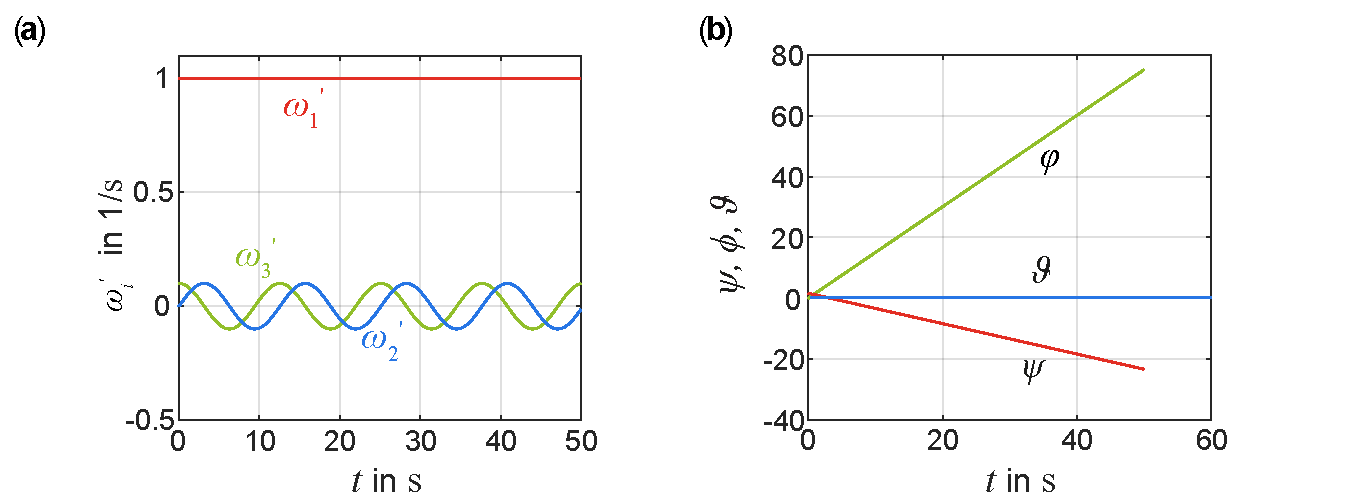
\includegraphics[width=\textwidth]{SymmKreiselEulerWinkel.pdf}
\captionof{figure}[Dynamik der Nutation eines kr�ftefreien symmetrischen Kreisels.]{Dynamik der Nutation eines kr�ftefreien symmetrischen Kreisels. \fa Zeitliche Entwicklung von $\vec{\omega}$, \fb Zeitliche Entwicklung der Euler-Winkel. Parameter: $J_1 = J_2 = \SI{1}{\kg\metre\squared}\,,\, J_3 = \SI{1.5}{\kg\metre\squared}$.} \label{abb:bew_SymmKreiselEulerWinkel}
\end{center}
\end{example}
%Ende BEISPIEL %%%%%%%%%%%%%%%%%%%%%%%%%%%%%%%%%%%%%%%%%%%%%%%%%%%%%%%%%%%%%%%%%%%%%%%%%%%%%%%%%%
Wie wir gesehen haben, gibt es im raumfesten System $\vec{\Sigma}$ neben der Nutation der Figurenachse um die Drehimpulsachse auch 
eine Drehung der Achse der Winkelgeschwindigkeit $\vec{\omega}$ um die $\vec{L}$-Achse. Diese rotiert auf dem sogenannten \emph{Rastpolkegel}, der den 
�ffnungswinkel 
\begin{align}
	\alpha_\text{RPK} = \arctan{\frac{\omega_\perp'}{\omega_3'}} = \arctan{\frac{\sqrt{{\omega_1'}^2+{\omega_2'}^2}}{\omega_3'}} \label{eq:bew_Nutation_alphaRPK}
\end{align}
hat. Im k�rperfesten System $\vec{\Sigma}'$ hingegen rotiert diese $\vec{\omega}$-Achse um die Figurenachse auf dem \emph{Polkegel}, dessen �ffnungswinkel $\alpha_\text{PK}$ durch den Winkel zwischen den Komponenten $L_3 \,\vecpeZ$ und $\vec{\omega}_3'\,\vecpeZ$ gegeben ist: 
\begin{align}
	\alpha_\text{PK} = \arctan{\frac{\Omega\,\sin\vartheta_\text{N}}{\Omega' + \Omega\,\cos\vartheta_\text{N}}}\,. \label{eq:bew_Nutation_alphaPK}
\end{align}
Anschaulich kann man sich das so vorstellen, dass der Polkegel auf dem Rastpolkegel abrollt, wobei die
Kontaktlinie beider Kegel gerade der Achse der Winkelgeschwindigkeit entspricht (die dort quasi \anf{rastet}, daher der Name Rastpolkegel).
Diese komplizierten Bewegungen der einzelnen Achsen sind in \figref{bew_KfSymmKrNutation}b und c gezeigt.
Sie sind gewisserma�en notwendig, damit die Drehimpulserhaltung gew�hrleistet ist.
Die einzelnen Bewegungen und ihr Zusammenhang mit den Euler-Winkeln ist noch einmal in Tabelle
\ref{tab:bew_KfSymmKrNutation} zusammengefasst.

\begin{table}%
\caption[�bersicht �ber die Rotationsbewegungen des kr�ftefreien symmetrischen Kreisels.]{�bersicht �ber die Rotationsbewegungen des kr�ftefreien symmetrischen Kreisels.}
\begin{tabular}{L{2.0cm}L{1.9cm}@{\ }C{0.7cm}L{1.2cm}C{1.0cm}L{5.0cm}}
\hline\noalign{\smallskip}
Kegel & �ffnungswinkel & KOS & Rotation &Euler-Winkel & Rotationsfrequenz  \\
\noalign{\smallskip}\svhline\noalign{\smallskip}
Nutationskegel\footnote{In manchen B�chern und vor allem in der angels�chsischen Literatur wird der Nutationskegel\index{Nutationskegel}\index{Polkegel}\index{Rastpolkegel} auch als Pr�zessionskegel\index{Pr�zessionskegel} bezeichnet. Wir benutzen den Begriff Pr�zession ausschlie�lich f�r den schweren Kegel, \dh einem nicht kr�ftefreien Kegel (\kap{bew_Kreisel_schwer}).} & $\vartheta_\text{N}$\hfill\eqref{eq:bew_Nutationswinkel}
               & $\vec{\Sigma}'$ & $\vec{f}$ um $\vec{L}$      &           & $\Omega'=\omega_\perp'/\sin\vartheta_\text{N}$\\
Nutationskegel & $\vartheta_\text{N}$\hfill\eqref{eq:bew_Nutationswinkel}   
               & $\vec{\Sigma}\phantom' $ & $\vec{L}$ um $\vec{F}$      &           & $\Omega = L/J_{12} = J_3\,\omega_3' /\lk J_{12}\,\cos\vartheta_\text{N} \rk$ \\
Rastpolkegel   & $\alpha_\text{RPK}$\hfill\eqref{eq:bew_Nutation_alphaRPK} 
               & $\vec{\Sigma}\phantom' $ & $\vec{\omega}'$ um $\vec{f}$& $\varphi$ & $\Omega = L/J_{12} = J_3\,\omega_3  /\lk J_{12}\,\cos\vartheta_\text{N} \rk$ \\
Polkegel       & $\alpha_\text{PK}$\hfill\eqref{eq:bew_Nutation_alphaPK}  
               & $\vec{\Sigma}'$ & $\vec{\omega}$ um $\vec{L}$ & $\psi$    & $\Omega'=\omega_\perp'/\sin\vartheta_\text{N}$\\
\noalign{\smallskip}\hline\noalign{\smallskip}
\end{tabular}
\label{tab:bew_KfSymmKrNutation}
\end{table}

Im Allgemeinen wird bei einem symmetrischen Kegel, der in Rotation versetzt wird,
die Figurenachse mit der Drehimpulsachse zusammenfallen.
Man kann sich aber ein Auseinanderfallen dieser beiden Achsen \zb dadurch entstanden denken,
dass die urspr�nglich kollineare Ausrichtung von Drehimpuls- und Figurenachse
durch einen Sto� oder eine interne Massenverlagerung gest�rt wird.
Letzteres ist \zb bei der Erde der Fall.
Ihre Symmetrieachse f�llt wegen sich ver�ndernder Masseverteilungen (\zb durch Vegetationsperioden)
nicht genau mit ihrer Drehachse zusammen. Letztere verl�uft durch den Schwerpunkt des Erdk�rpers.
Deswegen \anf{taumelt} (nutiert) auch der Erdk�rper (\probref{bew_Polbewegung}).%
\footnote{Wir werden im nachfolgenden Kapitel sehen, dass noch andere, wesentlich gr��ere Effekte auf den Erdkreisel wirken.}

\subsubsection{Bewegung eines schweren symmetrischen Kreisels} \index{Kreisel!schwerer!|textbf}\label{kap:bew_Kreisel_schwer}

Unter einem \anf{schweren} Kreisel versteht man einen starren K�rper, dessen Unterst�tzungs\-punkt nicht mit dem Schwerpunkt des K�rpers �bereinstimmt. %Wir haben bei diesem folglich ein von Null verschiedenes Drehmoment. 
Befindet sich ein solcher Kreisel in einem Schwerefeld so bewirkt die Gewichtskraft ein Drehmoment $\vec{M}_\text{D}$, welches die Bewegung des Kreisels beeinflusst (\figref{bew_SchwererKreisel}). 

In die Kreiselgleichungen \eqref{eq:bew_EulerGleichung02} muss nun das Drehmoment 
%\textit{Segway}\footnote{Der Segway Personal Transporter ist ein elektrisch angetriebenes Einpersonen-Fahrzeug mit nur zwei auf derselben (geometrischen) Achse liegenden R�dern, das sich durch eine elektronische Antriebsregelung selbst in Balance h�lt. Ein elektronischer Regelkreis l�sst den Segway automatisch in die Richtung fahren, in die sich der Fahrer lehnt. Sobald die Kreisel-Neigungssensoren (Halbleiter-Gyroskope) registrieren, dass sich der Fahrer nach vorne oder hinten neigt, drehen die R�der in die entsprechende Richtung.}, 
\begin{equation*}
  \MD = \vec{s} \times m \,\vec{g} = s \,\vecpeZ \times m \,\vec{g}
\end{equation*}
bez�glich des Unterst�tzungspunktes eingesetzt werden. Dies kann im Allgemeinen eine sehr aufwendige L�sung erfordern.

%\begin{figure}
  %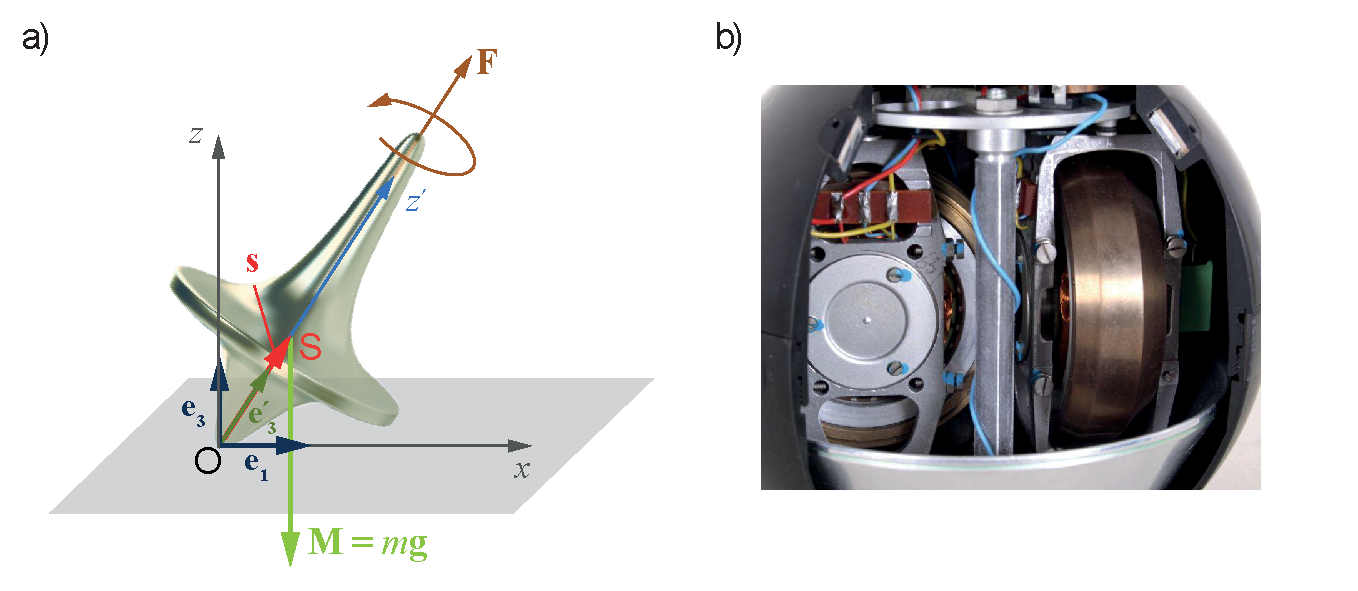
\includegraphics[width=\textwidth]{SchwererKreisel01.pdf}
  %\caption[Schwerer symmetrischer Kreisel.]{Beispiele eines schweren
    %symmetrischen Kreisels. a) Der Unterst�tzungspunkt (hier die Auflage auf
    %dem Boden) stimmt nicht mit dem Schwerpunkt �berein. Dadurch wirkt
    %ein Drehmoment auf den Kreisel, das die Bewegung beeinflusst. Das Drehmoment greift am Schwerpunkt an und zeigt in die Papierebene hinein. b) Anwendung des Prinzips des schweren Kreisels im maritimen Kreiselkompass. Einblick in einen Kreiselkompass der Firma  Ansch�tz-Raytheon.
    %}\label{abb:bew_SchwererKreisel}
%\end{figure}
\begin{figure}
  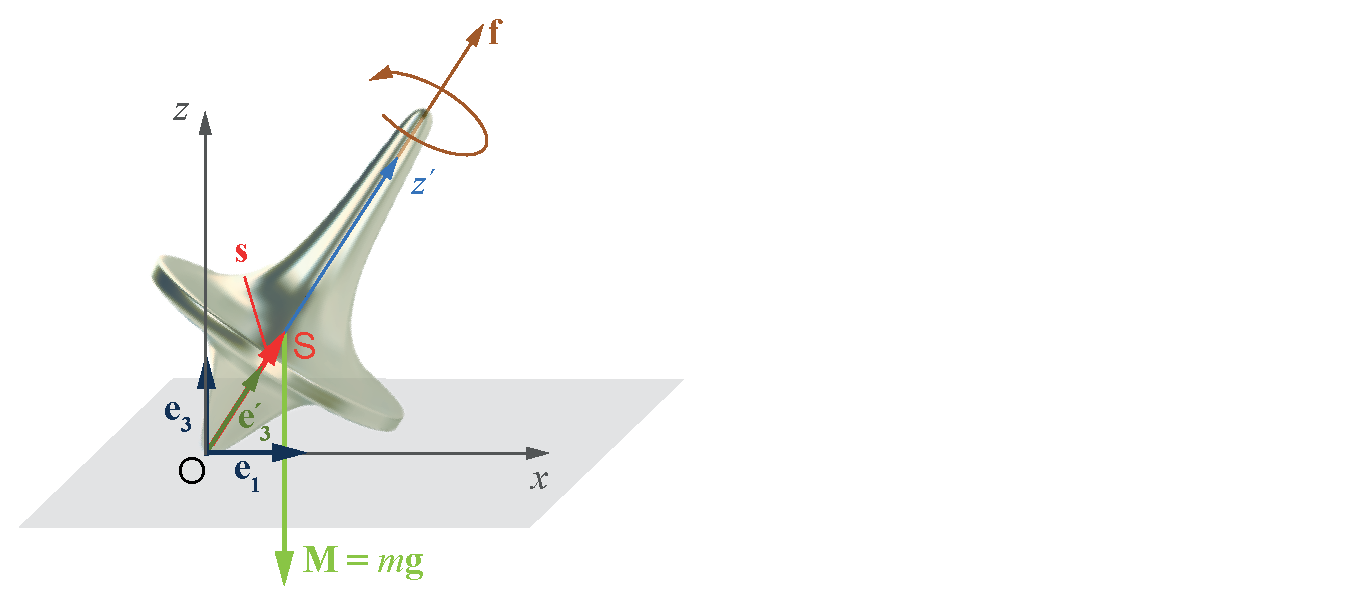
\includegraphics[width=\textwidth]{SchwererKreisel.pdf}
  \caption[Schwerer symmetrischer Kreisel.]{Beispiel  eines schweren
    symmetrischen Kreisels. Der Unterst�tzungspunkt (hier die Auflage auf
    dem Boden) stimmt nicht mit dem Schwerpunkt �berein. Dadurch wirkt
    ein Drehmoment auf den Kreisel, das die Bewegung beeinflusst. Das Drehmoment greift am Schwerpunkt an und zeigt in die Papierebene hinein.}\label{abb:bew_SchwererKreisel}
\end{figure}

Wir wollen wieder einen besonders interessanten Spezialfall betrachten. Dazu gehen wir davon aus, dass die Figurenachse $\vec{f}=\vecpeZ$,\,$\vec{\omega}$ und $\vec{L}$ parallel zueinander liegen und dies im wesentlichen auch so bleibt, weil das Drehmoment nur eine kleine �nderung der Bewegung hervorruft. Mit dieser Annahme steht das Drehmoment wegen
	\[\MD = m \, g \,\vecpeZ \times \veceZ \;\propto \;\vec{L} \times \veceZ\]
senkrecht zum Drehimpuls, da es senkrecht zur Figurenachse gerichtet ist. Die Darstellung in \figref{bew_SchwererKrPraezessionL}a verdeutlicht dies.

\begin{figure}
  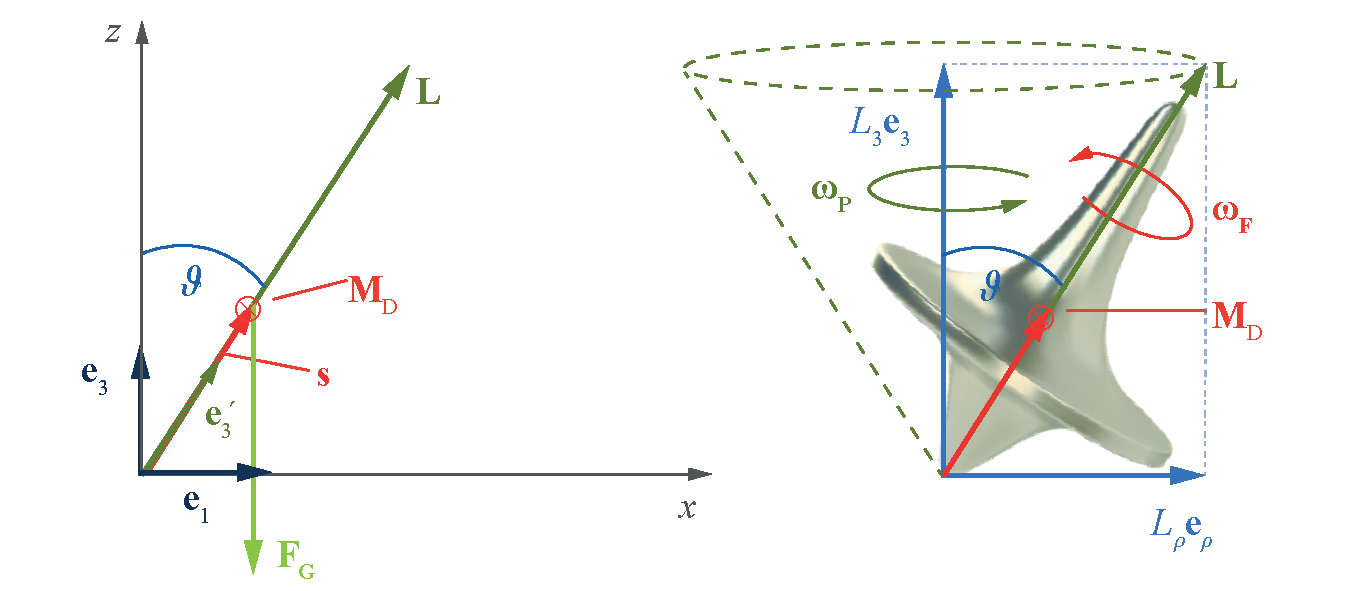
\includegraphics[width=\textwidth]{SchwererKrPraezessionL.pdf}
  \caption[Drehmoment auf einen schweren Kreisel.]{Pr�zession aufgrund eines
    Drehmoments am schweren symmetrischen Kreisel f�r den nutationsfreien
    Spezialfall, in dem der Drehimpuls $\vec{L}$, die Rotationsachse
    $\vec{\omega}$ und die Figurenachse $\vec{f}=\vecpeZ$ aufeinander liegen.
    Durch die Gewichtskraft wirkt ein Drehmoment, das senkrecht zum Drehimpuls
    liegt und dessen Richtung �ndert. Es ergibt sich eine Rotation des
    Drehimpulses um die $\veceZ$-Achse. 
		%c) Pr�zession und Nutation des schweren symmetrischen Kreisels �berlagert.
    \label{abb:bew_SchwererKrPraezessionL}}
\end{figure}
%
Das Drehmoment folgt aus
\begin{equation*}
  \MD = \vec{s} \times \vec{F}_\mathrm{G} = \left ( s \sin\vartheta\,
    \vec{e}_\varrho + s \cos \vartheta \, \veceZ \right ) \times
  (-mg)\,\veceZ = m\,g\,s\sin\vartheta \, \vec{e}_\varphi \; ,
\end{equation*}
wobei hier Zylinderkoordinaten ($\vec{e}_\varrho, \vec{e}_\varphi, \vec{e}_z = \vec{e}_3$) f�r das raumfeste Koordinatensystems $\vec{\Sigma}$
eingef�hrt wurden. Die Aufteilung des Drehimpulses erfolgt in eine Komponente parallel zur
$\veceZ$-Achse und eine senkrecht dazu. In Zylinderkoordinaten l�sst
sich das schreiben als (\figref{bew_SchwererKrPraezessionL}b)
\begin{align*}
  \vec{L} &= L_\varrho \,\vec{e}_\varrho + L_3 \,\veceZ \,,
            \intertext{woraus sich f�r die Zeitableitung ergibt}
            \frac{\D}{\D t} \vec{L} &= \dot{L}_\varrho \, \vec{e}_\varrho +  L_\varrho\,\dot{\vec{e}}_\varrho + \dot{L}_3 \,\veceZ
                                      = \dot{L}_\varrho \,\vec{e}_\varrho +  L_\varrho \,\dot{\varphi} \, \vec{e}_\varphi + \dot{L}_3 \,\veceZ \\
          &\overset{!}{=} \MD = m\,g\,s\, \sin\vartheta \, \vec{e}_\varphi = \text{const} \, \vec{e}_\varphi\; .
\end{align*}
Daraus liest man sofort wegen $\D (L^2) / \D t = 2\,\vec{L}\,\D \vec{L}/\D t $ ab, dass auch $ L = \D \left| \vec{L}\right|/\D t = 0$ und 
\begin{equation}
  \dot{\varphi} = \frac{m \,g \,s \,\sin\vartheta}{L_\varrho} = \frac{m\, g\, s\, \sin\vartheta}{\left | \vec{L} \right | \sin\vartheta} = \frac{m\, g\, s}{\left | \vec{L} \right |} = \frac{m\, g\, s}{J_3 \,\omega_F} = \con  = \omega_P \label{eq:bew_SchwererKr01}
\end{equation}
gelten. Hier ist wobei $\omega_\text{F}$ die Kreisfrequenz der schnellen Drehbewegung um die
Figurenachse. Die Komponenten $L_\varrho$ und $L_3$ und damit der Betrag
des Drehimpulses sind, wie es sein muss, konstant.
Im betrachteten Spezialfall folgt die Figurenachse der Bewegung des
Drehimpulses und im Ergebnis erh�lt man eine Drehung des schweren symmetrischen
Kreisels mit der Winkelgeschwindigkeit
\begin{equation}
  \omega_P = \frac{m\, g\, s}{J_3\,\omega_\text{F}} \label{eq:bew_SchwererKr02}
\end{equation}
um die $\veceZ$-Achse. Diese Bewegung hei�t \emph{Pr�zession}\index{Pr�zession} und $\omega_P$ wird
\emph{Pr�zessionskreisfrequenz} oder oft auch kurz \emph{Pr�zessionsfrequenz}\index{Pr�zessionsfrequenz} genannt. Ausf�hrlicher, insbesondere �ber den hier
gew�hlten Spezialfall hinaus, erfolgt die Betrachtung in
\kap{bew_SchwererSymmKr}. Daf�r f�hren wir jedoch zun�chst den
Lagrange-Formalismus f�r den starren K�rper ein.

\subsection{Lagrange-Formalismus f�r einen Kreisel}\index{Lagrange-Formalismus} \label{kap:bew_Lagrange_StarrerK}

Der Lagrange-Formalismus f�r starre K�rper folgt in allen Punkten den in 
\kap{bew_lagrange_formalism} dargelegten Grundz�gen f�r Massepunkte.
Als besondere Zwangsbedingung kommt hinzu,
dass sich die Massepunkte des Systems nicht unabh�ngig voneinander
bewegen k�nnen.
Die einzigen verbleibenden Freiheitsgrade sind diejenigen,
die bereits durch die Betrachtung der kinetischen Energie in
\kap{bew_StarrerK_kin_Energie} offensichtlich wurden, n�mlich
die Position des Schwerpunkts $\vec{R}_S$ und die aktuelle Rotation
$\vec{\xi}$ des K�rpers.
Dabei entspricht die Rotation $\vec{\xi}$ drei
Freiheitsgraden und kann beispielsweise durch die Angabe einer Drehachse (2
Koordinaten) und eines Drehwinkels (1 Koordinate) oder durch die drei
Euler-Winkel beschrieben werden.
Insgesamt haben wir es also bei einem
freien starren K�rper mit sechs Freiheitsgraden zu tun.
Diese k�nnen
durch zus�tzliche Zwangsbedingungen (\zb Einspannen am Schwerpunkt und
somit $\vec{R}_S = \conv$) weiter eingeschr�nkt werden.

Gibt es keine weiteren Einschr�nkungen, sind geeignete generalisierte
Koordinaten bereits durch $\vec{R}_S$ und $\vec{\xi}$ gegeben.
F�r den allgemeinen freien starren K�rper erh�lt man die kinetische
Energie nach Gleichungen \eqref{eq:bew_Kin_Energie_starrerK} und
\eqref{eq:bew_Trot_starrerK}, n�mlich
\begin{equation}
  T = T_\mathrm{trans} + T_\mathrm{rot}
  = \frac{1}{2} M\,{\vec{V}_S}^2 +  \frac{1}{2} \vec{\omega}^T \underline{\vec{\Theta}} \,\vec{\omega} 
  \label{eq:bew_Lagrange_starrerK1}
\end{equation}
mit $\vec{V}_S = \dot{\vec{R}}_S$ und $\vec{\omega} = \dot{\vec{\xi}}$.

Das Potential kann im allgemeinen Fall sowohl von der Position des
Schwerpunkts $\vec{R}_S$ als auch der Lage des K�rpers $\vec{\xi}$
abh�ngen, sodass man die allgemeine Lagrange-Funktion
\begin{equation}
  \mathcal{L}(\vec{R}_S,\vec{\xi},\vec{V}_S,\vec{\omega}) =
  T(\vec{V}_S,\vec{\omega}) - U(\vec{R}_S,\vec{\xi})
= \frac{1}{2} M\,{\vec{V}_S}^2 +  \frac{1}{2} \vec{\omega}^T \underline{\vec{\Theta}} \,\vec{\omega} - U(\vec{R}_S,\vec{\xi})
\end{equation}
erh�lt.
In vielen Anwendungen ist man jedoch wieder nicht an der Bewegung
des Schwerpunkts interessiert.
Das gilt insbesondere f�r F�lle, in denen
der starre K�rper keine Translation ausf�hrt.
In diesem Fall reduziert sich die Lagrange-Funktion auf
\begin{equation}
  \mathcal{L}(\vec{\xi},\vec{\omega}) = T(\vec{\omega}) - U(\vec{\xi}) =
  \frac{1}{2} \,\vec{\omega}^T \underline{\vec{\Theta}} \,\vec{\omega} - U(\vec{\xi})
  ~.   \label{eq:bew_Lagrange_starrerK2}
\end{equation}
F�r viele Anwendungen stellen die in \kap{bew_EulerWinkel}
eingef�hrten Euler-Winkel eine geeignete und elegante Darstellung bereit.
Mit der Annahme, dass das k�rperfeste Koordinatensystem ein Hauptachsensystem
ist, betr�gt die kinetische Energie
\begin{equation*}
  T(\vec{\omega}) = \frac{1}{2} \lk J_1 \omega_1'^2 + J_2 \omega_2'^2
    + J_3 \omega_3'^2 \rk
\end{equation*}
\bzw mithilfe der Euler-Winkel \eqref{eq:bew_EulerWinkel} ausgedr�ckt
\begin{equation*}
  T(\vec{\omega}) = \frac{1}{2} \left ( J_1\,(\dot{\varphi} \sin\vartheta \sin
    \psi + \dot{\vartheta} \cos\psi)^2 + J_2 \,(\dot{\varphi} \sin\vartheta \cos
    \psi - \dot{\vartheta} \sin\psi)^2
    + J_3 \,(\dot{\varphi} \cos\vartheta + \dot{\psi})^2 \right ) \,. 
\end{equation*}
Die Lagrange-Funktion lautet dann
\begin{multline}
  \mathcal{L}(\varphi,\vartheta,\psi,\dot{\varphi},\dot{\vartheta},\dot{\psi})
  = \frac{1}{2} \Bigl ( J_1 (\dot{\varphi} \sin\vartheta \sin
    \psi + \dot{\vartheta} \cos\psi)^2 + J_2 (\dot{\varphi} \sin\vartheta \cos
    \psi - \dot{\vartheta} \sin\psi)^2 \\
    + J_3 (\dot{\varphi} \cos\vartheta + \dot{\psi})^2 \Bigr )
  -U(\varphi,\vartheta,\psi) ~ .  \label{eq:bew_Lagrange_starrerK3}
\end{multline}

\subsection{Dynamik des schweren symmetrischen Kreisels}\index{Kreisel!schwerer symmetrischer} \label{kap:bew_SchwererSymmKr}

Eine typische Anwendung, die den Vorteil des Lagrange-Formalismus sichtbar
macht, ist der symmetrische schwere Kreisel aus
\figref{bew_SchwererKreisel}.
Ausgedr�ckt in den Euler-Winkeln lautet seine Lagrange-Funktion mit $J_{12}=J_1=J_2$
\begin{equation}
  \mathcal{L} = \frac{J_{12}}{2}\, \left ( \dot{\varphi}^2 \sin^2\vartheta + \dot{\vartheta}^2
\right ) + \frac{J_3}{2}\, \left (\dot{\varphi} \cos\vartheta + \dot{\psi}
\right )^2 - m\,g\,s\,\cos{\vartheta} \,.  \label{eq:bew_Lagrange_starrerK4}
  \end{equation}
  Die Koordinaten $\varphi$ und $\psi$ sind zyklisch (das Potential h�ngt nur von $\vartheta$ ab)
  und f�hren direkt auf die beiden Erhaltungsgr��en
  \begin{align*}
    p_\psi &= \frac{\partial \mathcal{L}}{\partial \dot{\psi}} =
    J_3 \left ( \dot{\varphi} \cos\vartheta + \dot{\psi} \right )
             = J_3 \,\omega_3 = \con
    \intertext{und}
    p_\varphi &= \frac{\partial \mathcal{L}}{\partial \dot{\varphi}}
    = J_{12} \, \dot{\varphi} \sin^2\vartheta + J_3 \left ( \dot{\varphi}
                \cos\vartheta + \dot{\psi} \right ) \cos\vartheta =
    J_{12}\, \dot{\varphi} \sin^2\vartheta + J_3\,\omega_3 \cos\vartheta = \con\,.
  \end{align*}
  Aus ihnen lassen sich die Zeitentwicklungen der Winkel $\varphi$ und $\psi$ zu
  \begin{align}
	\begin{split}
    \dot{\varphi} &= \frac{p_\varphi - J_3 \, \omega_3 \cos\vartheta}{J_{12} \sin^2
    \vartheta} ~ , \\ 
    \dot{\psi} &= \omega_3 - \frac{p_\varphi - J_3 \, \omega_3 \cos\vartheta}
    {J_{12} \sin^2 \vartheta} \cos\vartheta ~ 
	\end{split} \label{eq:bew_Lagrange_starrerK4a}
  \end{align}
  berechnen. Eine weitere Erhaltungsgr��e ist die Gesamtenergie $E = T + U$.
  Setzt man in diese das Wissen \eqref{eq:bew_Lagrange_starrerK4a} �ber $\dot{\varphi}$ und $\dot{\psi}$ 
	 ein, erh�lt man
  \begin{align}
    E &= \frac{J_{12}}{2} \,\left ( \dot{\varphi}^2 \sin^2\vartheta
      + \dot{\vartheta}^2 \right )
    + \frac{J_3}{2}\, \left (\dot{\varphi} \cos\vartheta + \dot{\psi} \right )^2
    + mg s \cos{\vartheta} \nonumber \\
    &=  \frac{J_{12}}{2} \,\dot{\vartheta}^2 + \underbrace{\frac{\left ( p_\varphi - J_3 \,\omega_3\,
        \cos\vartheta \right )^2}{2 J_{12} \,\sin^2\vartheta}
      + \frac{J_3}{2}\, \omega_3^2 + m\,g\,s\,\cos{\vartheta}}_{U_\mathrm{eff}(\vartheta)}
      = \frac{J_{12}}{2}\, \dot{\vartheta}^2 + U_\mathrm{eff}(\vartheta) ~.
			\label{eq:bew_Lagrange_starrerK4b}
  \end{align}
Die Energie h�ngt nur noch von $\dot{\vartheta}$ und einem effektiven Potential $U_\mathrm{eff}(\vartheta)$ ab, das wiederum eine Funktion nur von $\vartheta$ ist.
Dieses Potential hat f�r die Kreiselparameter
$m=\SI{1}{\kg}$ (Masse), $J_3 = \SI{0.6}{\kg\metre\squared}$, $J_{12} = \SI{0.4}{\kg\metre\squared}$ (Tr�gheitsmomente), $\omega_3 = \SI{1}{\per\s}$ (Rotationskreisfrequenz der Figurenachse), $s=\SI{20}{\centi\metre}$ (Abstand des Auflagepunktes zum Schwerpunkt) und dem
Verh�ltnis der zyklischen \anf{Impulse}
		\[\frac{p_\varphi}{p_\psi} = \frac{p_\varphi}{J_3\,\omega_3} = \frac{1}{3}
	\] die in \figref{bew_SchwererKrPot} dargestellte Form.
  Daraus gewinnt man eine isolierte Bewegungsgleichung f�r $\vartheta$,
  \begin{equation}
    J_{12} \ddot{\vartheta} = \frac{\left ( p_\varphi - J_3\, \omega_3
        \cos\vartheta \right )^2}{J_{12} \sin^3\vartheta} \cos\vartheta
    -J_3\, \omega_3 \,\frac{p_\varphi-J_3\, \omega_3\cos\vartheta}{J_{12}\sin\vartheta}
    + m\,g\,s\,\sin\vartheta \; . \label{eq:bew_Lagrange_starrerK4c}
  \end{equation}
  Diese Gleichung kann im Allgemeinen nur numerisch gel�st werden.
  F�r verschiedene Gesamtenergien $E$, die durch die verschiedenen Linien im Potentialdiagramm dargestellt 
	sind, haben wir die Bewegungsabl�ufe im \mscr{} \mlbewref{SchwererKreiselPraez02.m}
  f�r den Winkel des Drehimpulses zur $z$-Achse (dem Euler-Winkel $\vartheta$) beispielhaft berechnet
  und in \figref{bew_SchwererKrPtheta} dargestellt. 

\begin{figure}
\begin{minipage}{\textwidth}
\leftfigure{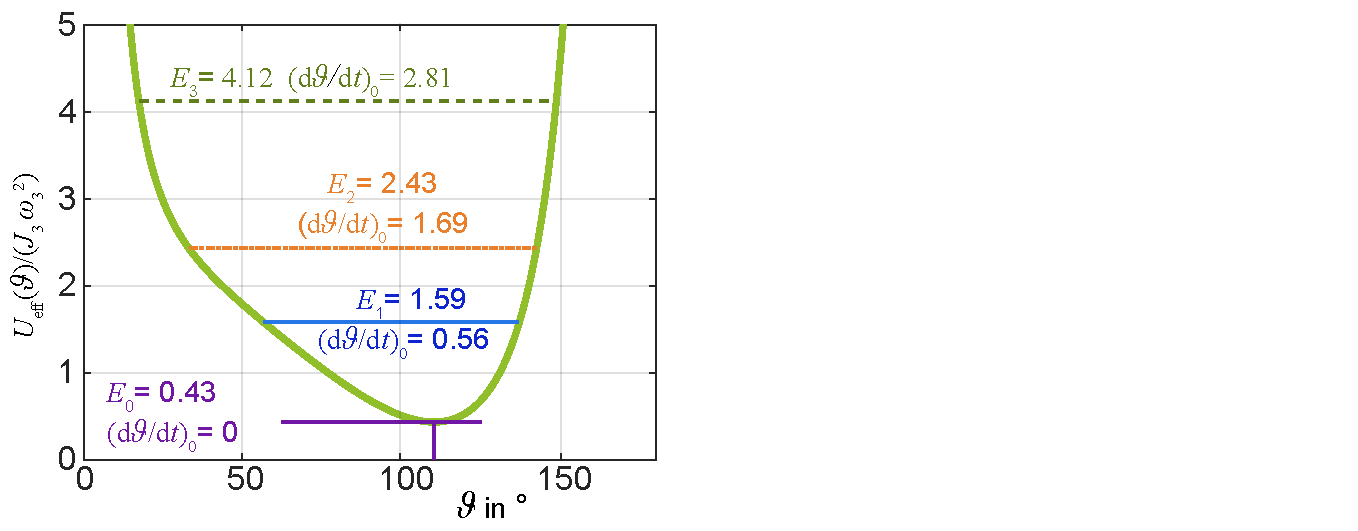
\includegraphics[width=0.9\textwidth]{SchwererKrPot.pdf}}%
\hspace{\fill}
\rightfigure{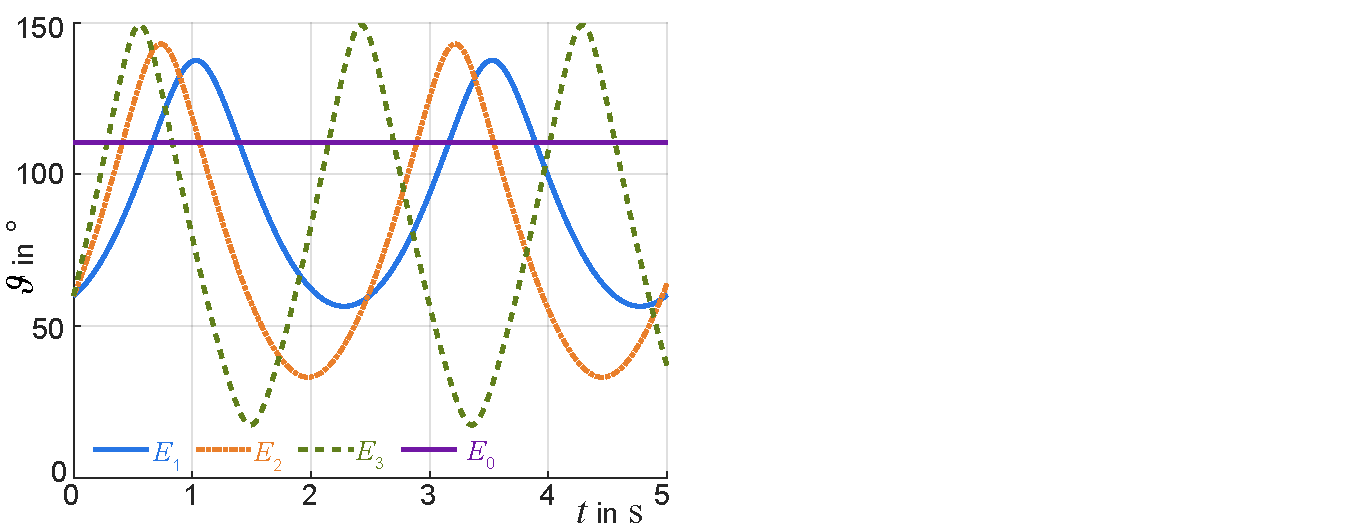
\includegraphics[width=0.9\textwidth]{SchwererKrPtheta.pdf}}
\leftcaption[Effektives Potential eines schweren Kreisels.]{Effektives Potential eines schweren Kreisels als Funktion des Euler-Winkels $\vartheta$.} \label{abb:bew_SchwererKrPot}
\rightcaption[Dynamik des Euler-Winkels $\vartheta$ beim schweren Kreisel.]{Dynamik des Euler-Winkels $\vartheta$ beim schweren Kreisel f�r verschiedene Energien (Werte aus Abb.\ \figref{bew_SchwererKrPot}).}\label{abb:bew_SchwererKrPtheta}
\end{minipage}
\end{figure}

  Man erkennt deutlich, wie die Bewegung am linken und rechten Rand des
  Potentials umkehrt. Der Neigungswinkel des Kreisels vollf�hrt eine periodische
  Bewegung zwischen diesen Extremwerten, die bei geringer Energie noch nahezu harmonisch ist,
  f�r h�here Energien aufgrund der Steilheit des Potentials aber in nick�hnliche Bewegungen �bergeht.
  Da der Drehimpulsvektor in diesem Fall nicht mit der Figurenachse und der Richtung der Winkelgeschwindigkeit $\vec{\omega}$ 
  �bereinstimmt, ist die Wirkung des Drehmoments mit einer Nutation\index{Nutation} �berlagert
  und die gesamte Bewegung des Kreisels inklusive der Ver�nderungen von $\psi$ und $\varphi$ relativ kompliziert.
	
\subsubsection{Schwerer Kreisel ohne Nutation}\label{kap:bew_SchwererSymmKr_O_Nutation}

  Wir k�nnen zun�chst f�r sehr geringe Energien diese zus�tzliche Nutationsbewegung vernachl�ssigen und erhalten  eine reine Pr�zession\index{Pr�zession!reine}%
  \footnote{Mitunter wird diese Pr�zession ohne begleitende Nutation auch \textit{regul�re Pr�zesssion}\index{Pr�zession!regul�re} oder \textbf{astronomische Pr�zession} genannt. Letzterer Begriff wird in \kap{bew_praez_erde} klarer werden. Zur unterschiedlichen Verwendung von Begrifflichkeiten siehe auch die Bemerkungen in \kap{bew_Kreisel_kraeftefrei}.},
  also eine Drehung der Drehimpulsachse des Kreisels im Raum durch die Wirkung
  des Drehmoments. Diese erh�lt man exakt als Spezialfall, wenn die
  Anfangsbedingungen so gew�hlt werden, dass $\vartheta(t=0)$ sich gerade im
  Minimum des effektiven Potentials befindet und damit die Anfangswinkelgeschwindigkeit $\dot{\vartheta}(t=0) = 0$ ist. 
  Das Ergebnis f�r diesen Spezialfall ist in \figref{bew_SchwererKrEuler_o_N} dargestellt,
  hierbei ergibt sich eine stabile
  Neigung $\vartheta$ der Figurenachse. Diese dreht sich jedoch durch
  das wirkende Drehmoment im Raum, wie an der linearen Zunahme von $\varphi$
  zu sehen ist. Dabei f�hrt der Kreisel eine Eigendrehung mit der
  Frequenz $\dot{\psi}$ um die Figurenachse aus.
\begin{figure}
\begin{minipage}{\textwidth}
\leftfigure{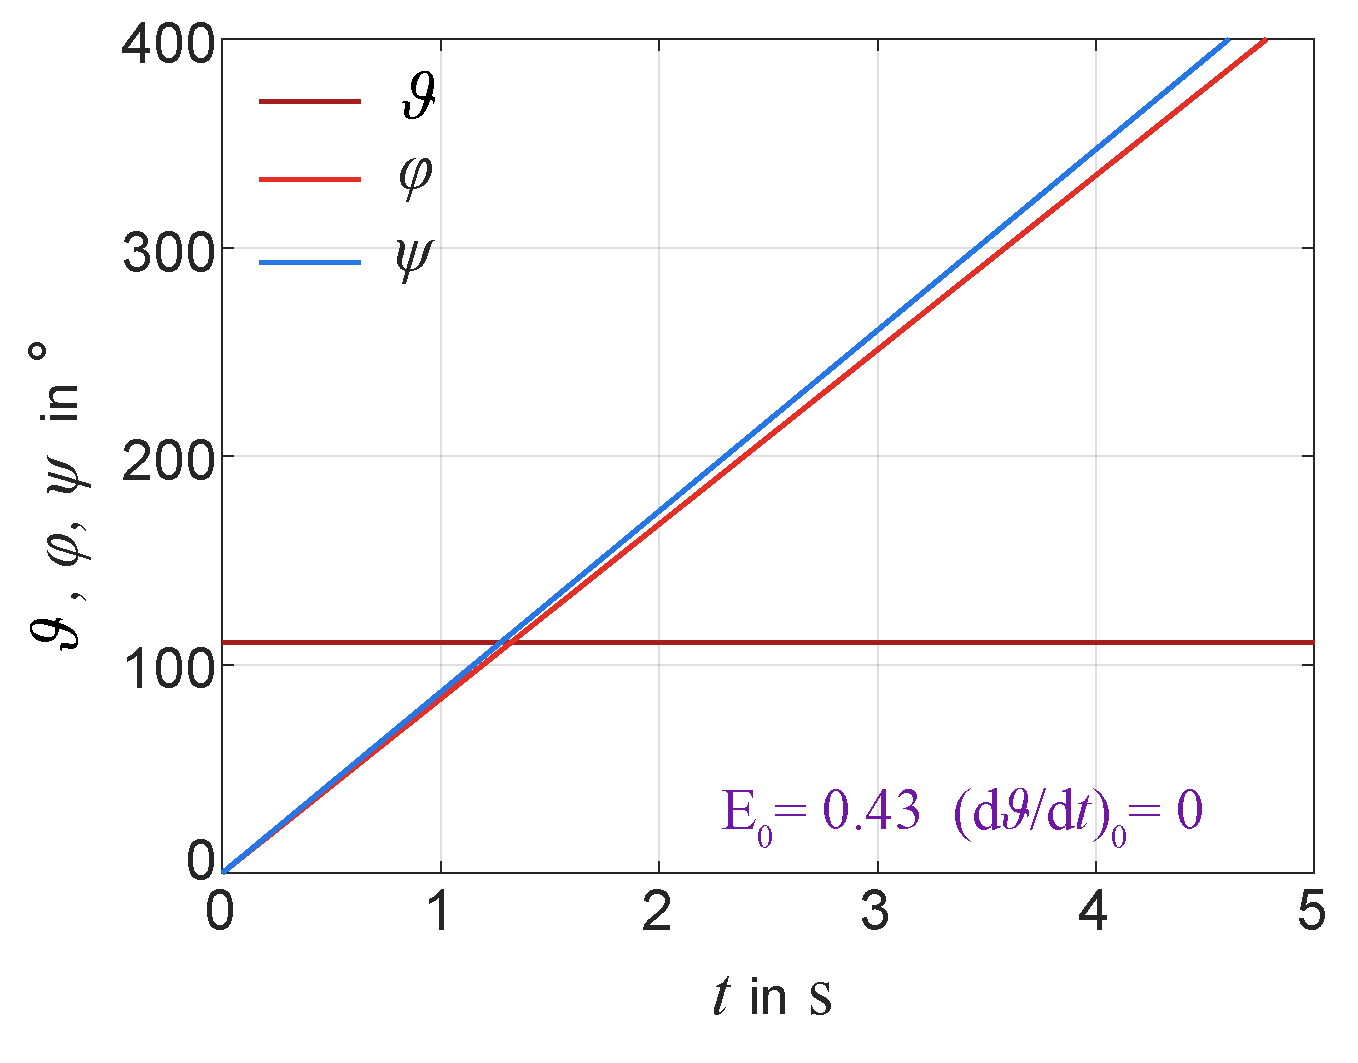
\includegraphics[width=0.45\textwidth]{SchwererKrEulerWohneN.pdf}}%
\hspace{\fill}
\rightfigure{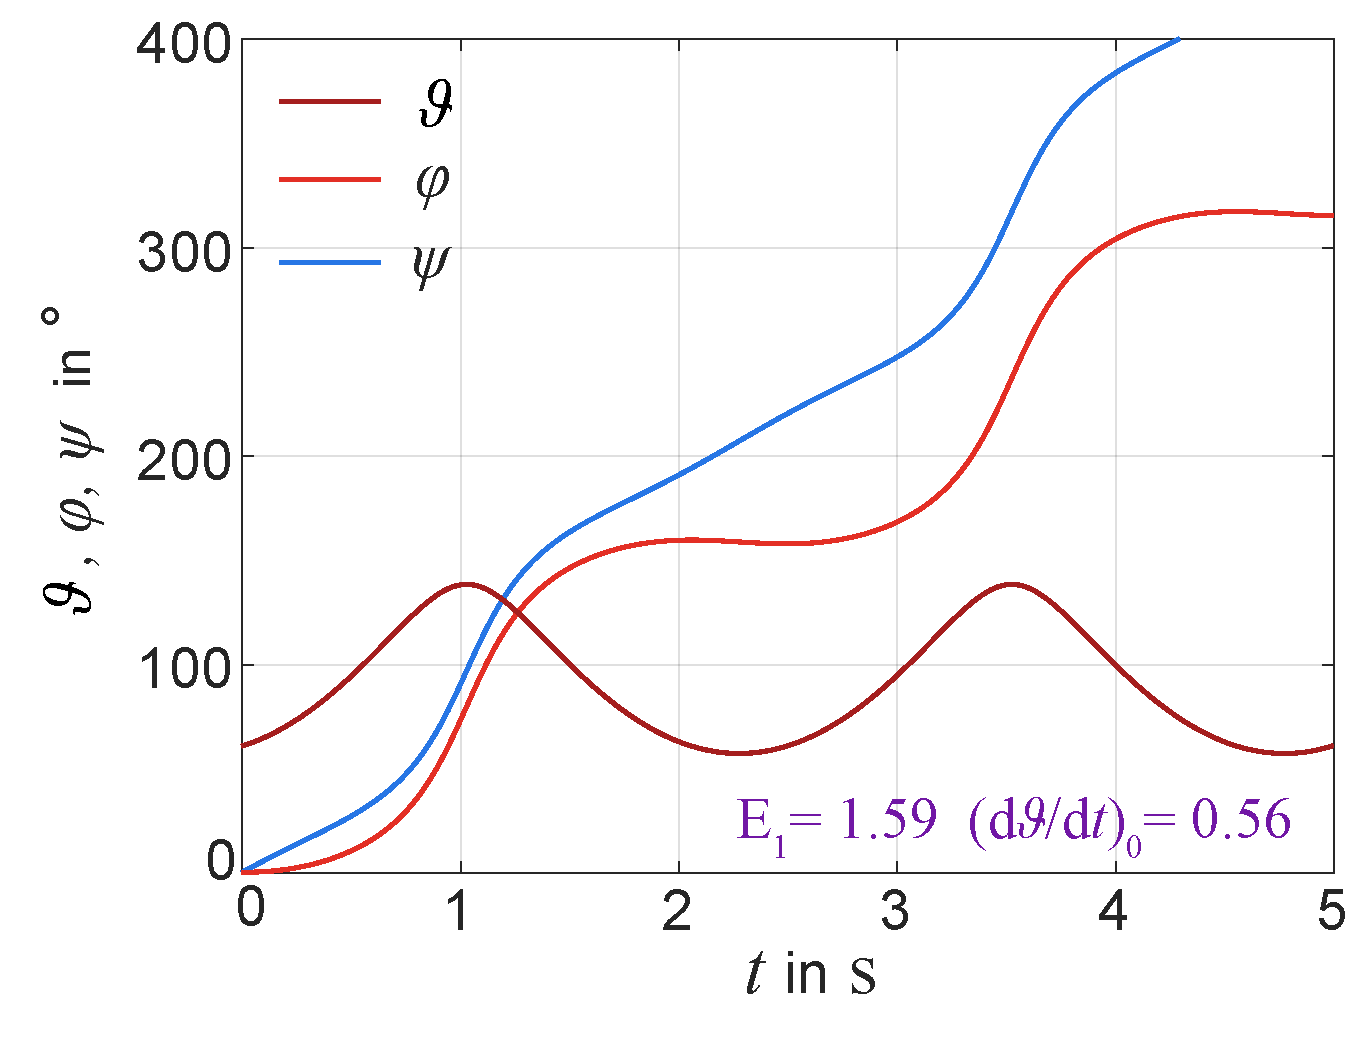
\includegraphics[width=0.45\textwidth]{SchwererKrEulerWmitN.pdf}}
\leftcaption[Dynamik der Euler-Winkel ohne Nutation.]{Dynamik der Euler-Winkel beim schweren Kreisel ohne Nutation.}\label{abb:bew_SchwererKrEuler_o_N}
\rightcaption[Dynamik der Euler-Winkel mit Nutation.]{Dynamik der Euler-Winkel beim schweren Kreisel mit Nutation.  Man erkennt am Winkel $\vartheta$ die Nickbewegungen der Nutation, ebenso ist die Eigendrehung um die Figurenachse von der Nutation �berlagert.} \label{abb:bew_SchwererKrEuler_m_N}
\end{minipage}
\end{figure}

\subsubsection{Schwerer Kreisel mit Nutation}\label{kap:bew_SchwererSymmKr_M_Nutation}

F�r den allgemeineren Fall mit  $\dot{\vartheta}(t=0) \neq 0$ ist der Bewegungsablauf im \mscr{} \mlbewref{SchwererKreiselSim.m} berechnet und in \figref{bew_SchwererKrEuler_m_N} dargestellt. Deutlich erkennbar sind die Nickbewegungen sowohl im Winkel $\vartheta$ als auch im Winkel $\varphi$.\\
Die Pr�zession und die Nutation des Erdkreisels spielen, wie bereist erw�hnt, 
in der Astronomie und der Himmelsmechanik (Band II, Kapitel 3) 
eine wichtige Rolle.
Da die Erde nahezu ein Rotationsellipsoid ist, bewirkt seine �quatorwulst, dass die Gezeitenkr�fte von Mond und Sonne ein Drehmoment erzeugen, das die Erdachse aufzurichten versucht und zur Pr�zession der Erdachse f�hrt (sogenannte \emph{lunisolare Pr�zession})\index{Pr�zession!lunisolare|textbf}.
Die Erdachse bewegt sich dadurch auf einem Pr�zessionskegel um eine Achse, die in etwa rechtwinklig auf der Ebene der Erdbahn um die Sonne steht. Der (nahezu) konstante Winkel zwischen der Erdachse und der Achse des Kegels ist die sogenannte Schiefe der Ekliptik; diese betr�gt derzeit etwa $23.44\degree$. Ein voller Umlauf dieser Pr�zessionsbewegung der Erdachse dauert etwa $\SI{25700}{}$ bis $\SI{25850}{}$ Jahre.\footnote{Die Beitr�ge zur astronomischen Pr�zession sind vor allem 
die Gezeitenkr�fte von Mond und Sonne, aber auch Beitr�ge anderer Planeten und Effekte der Allgemeinen Relativit�tstheorie.
Alle diese Betr�ge sind nicht konstant. Daher kann die Pr�zessionsperiode bisher nur auf etwa ein Jahrhundert angegeben werden.} (siehe \kap{bew_praez_erde}).


\clearpage
\section {Beispiele und Anwendungen zur Mechanik des starren K�rpers}\label{
kap:bew_anwendungen_II}

\subsection{Das physikalische Pendel und die Pendeluhr} \index{Pendel!physikalisches|textbf}\index{Pendel!Uhrenpendel} \label{kap:bew_pendel_phys}

Wir wollen nun mit dem Handwerkszeug von \kap{bew_starrer_koerper} einige Alltagsprobleme angehen.
Als erstes wollen wir die alte Pendeluhr aus Familienbesitz untersuchen.
In \probref{bew_traegheitsmomente} hatten wir ja schon das Gesamttr�gheitsmoment bez�glich der Pendelachse als Funktion der Position der Scheibenmasse und des Schiebereglers berechnet.
Bevor wir die Pendelperiode in Abh�ngigkeit dieser beider Parameter berechnen, soll zun�chst die Pendelgleichung eines beliebigen an einem Drehpunkt $O$ aufgeh�ngten starren K�rpers berechnet werden.
Wir betrachten dazu \figref{bew_PhysPendel}.

\begin{figure}
\begin{minipage}{\textwidth}
\leftfigure{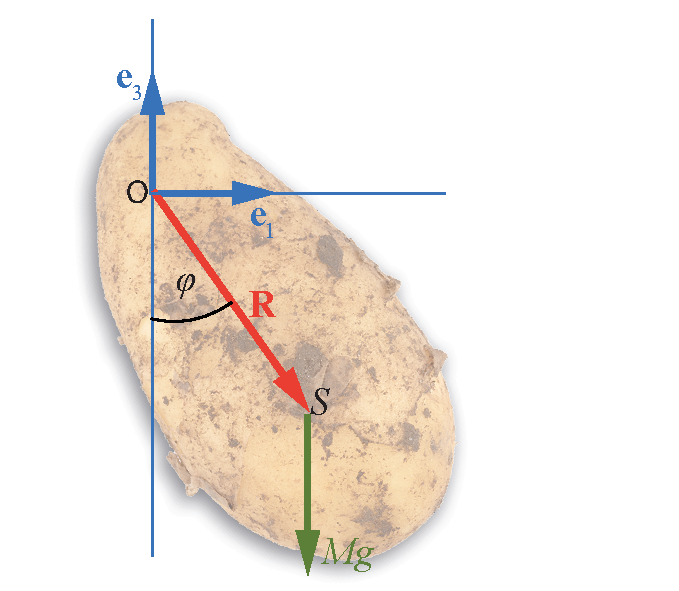
\includegraphics[width=0.5\textwidth]{PhysPendel.pdf}}%
\hspace{\fill}
\rightfigure{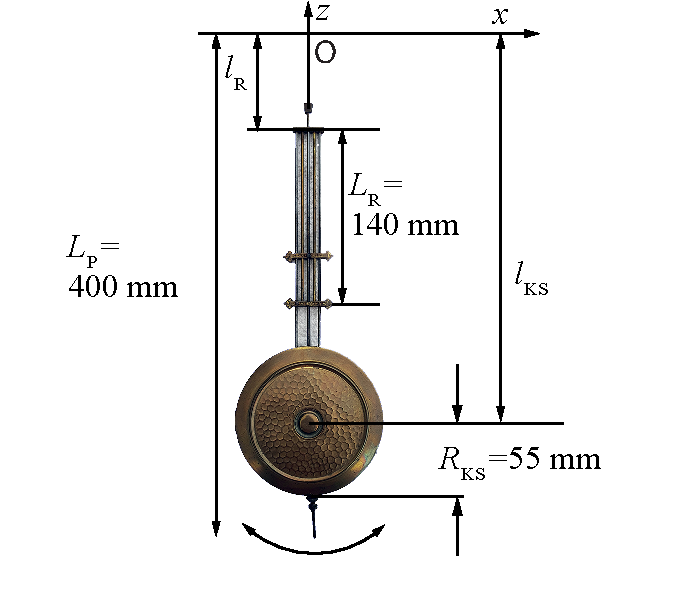
\includegraphics[width=0.5\textwidth]{Pendeluhr02.pdf}}
\leftcaption{Allgemeine Form eines physikalischen Pendels.} \label{abb:bew_PhysPendel}
\rightcaption[Realisierung des physikalischen Pendels als Pendeluhr.]{Realisierung des physikalischen Pendels als Pendeluhr.}\label{abb:bew_Pendeluhr02}
\end{minipage}
\end{figure}

Der starre K�rper (das physikalische Pendel) ist in $O$ aufgeh�ngt,
%/fixiert, => dann fehlte der rot. Fhg
der Schwerpunkt befindet sich in $S$.
Der K�rper habe das Tr�gheitsmoment $J_S$ bez�glich seines Schwerpunktes.
Dann k�nnen wir den Steinerschen Satz \eqref{eq:bew_SteinerSatz} anwenden und erhalten das Tr�gheitsmoment bez�glich der Drehachse $\veceY$ zu
        \begin{align*}
            J \, = \,J_S \,+ \,M\,R^2 \,,
        \end{align*}
worin $R$ der senkrechte Abstand der Drehachse zum Schwerpunkt ist. Das Drehmoment bez�glich der Achse $\veceY$ ist gegeben durch
        \begin{align*}
            \vec{M}_\text{D} &= \vec{R}\times \vec{F}_\text{G} = -M\,g\,\vec{R}\times\veceZ ~~\text{\bzw} ~~ {M}_\text{D} = -M\,g\,R\,\sin\varphi\,\veceY \,.
        \end{align*}
Nach dem Drehimpulssatz \eqref{eq:bew_DrehimpulsSatz} gilt
        \begin{align*}
           \frac{\D}{\D t}\,\lk J\,\omega_2\rk =  -M\,g\,R\,\sin\varphi \,,
        \end{align*}
worin $\omega_2$ die Rotationsfrequenz um die Achse $\veceY$ ist. Da $J$ konstant ist, k�nnen wir mit $\frac{\D \omega_2}{\D t} = \frac{\D}{\D t} \dot{\varphi} = \ddot{\varphi}$ schreiben:
        \begin{align}
            \ddot{\varphi} +\frac{M\,g\,R}{J} \,\sin\varphi = 0 \,. \label{eq:bew_PhysPendel01}
        \end{align}
Das ist eine Schwingungsgleichung, die f�r nicht zu gro�e Auslenkungen $\varphi$ in die Gleichung f�r den harmonischen Oszillator �bergeht:
        \begin{align}
            \ddot{\varphi} +\frac{M\,g\,R}{J}\,\varphi = 0 \,. \label{eq:bew_PhysPendel02}
        \end{align}
Hieraus berechnet sich die Schwingungsperiode des physikalischen Pendels zu
        \begin{align}
            T_\text{P} = 2\pi\sqrt{\frac{J}{M\,g\,R}} \,.\label{eq:bew_PhysPendel03}
        \end{align}
Die Schwingungsperiode des physikalischen Pendels ist also gegeben durch die Wurzel aus dem Quotienten von Tr�gheitsmoment und Drehmoment des K�rpers bezogen jeweils auf den Aufh�ngungspunkt. Da $R$ der Abstand des Schwerpunktes von der Aufh�ngung ist, haben wir f�r unsere Pendeluhr bei festgehaltenem Schieberegler und ver�nderlicher Pendelscheibe $l_\text{KS}$ also eine Abh�ngigkeit
\begin{align}
    T_\text{P}\lk l_\text{KS}, l_\text{R}\rk = 2\pi\sqrt{\frac{J\lk l_\text{KS}, l_\text{R}\rk}{M\,g\,R\lk l_\text{KS},l_\text{R}\rk}} \,, \label{eq:bew_PhysPendel04}
\end{align}
die wir im \mscr{} \mlbewref{Pendeluhr.m} berechnet und in \figref{bew_Pendeluhr03} f�r verschiedene Schiebereglerpositionen $l_\text{R}$ dargestellt haben. Man erkennt in \figref{bew_Pendeluhr03}, dass man eine hohe Einstellgenauigkeit hat.
Eine �nderung der Scheibenposition von $\SI{1}{\milli\metre}$ �ndert die Pendelperiode um \ca$\SI{1}{\milli\s}$,
die �nderung des Schiebereglers um $\SI{1}{\milli\metre}$ sogar nur um $\SI{0.1}{\milli\s}$.
Diese hohe Einstellgenauigkeit ist aber auch erforderlich,
denn bei einer Tagesl�nge von $\SI{86400}{\s}$
erzeugt eine Periodenabweichung von $\SI{0.5}{\milli\s}$
ein Nach- \bzw Vorgehen von \ca$\SI{45}{\s}$ pro Tag. 

\begin{figure}
  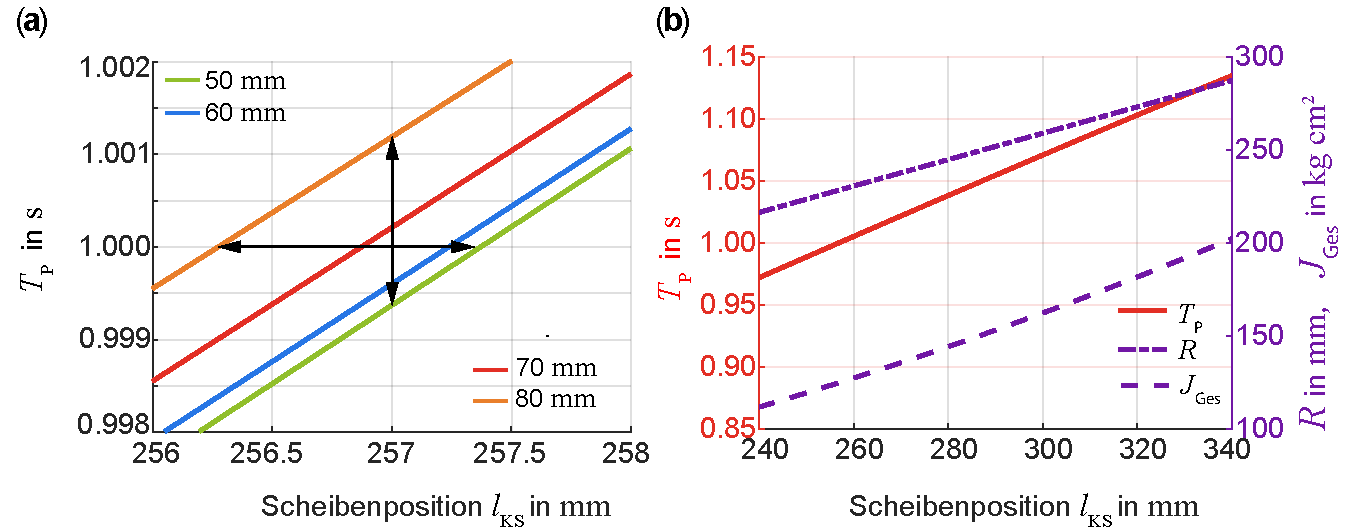
\includegraphics[width=\textwidth]{Pendeluhr03.pdf}
  \caption[Periodendauer einer Pendeluhr von den Einstellungen.]{Periodendauer einer Pendeluhr. \fa Abh�ngigkeit von den Einstellungen $l_\text{KS}$ (Abszisse) und $l_\text{R}$ (Parameter) und \fb Abh�ngigkeit vom Gesamtr�gheitsmoment $J_\text{Ges}$ und vom Abstand des Schwerpunkts $R$ von der Pendelaufh�ngung �ber einen gr��eren Bereich der Position der Pendelscheibe.}
    \label{abb:bew_Pendeluhr03}
\end{figure}

Wie man ferner erkennt, ist in guter N�herung
(aufgrund der Konstruktion (Massenverteilung) der Pendeluhr)
in der Umgebung der Normalstellung $T_\text{P} = \SI{1}{\second}$
ein linearer Zusammenhang $T_\text{P} =  C \,l_\text{KS}$ gegeben.
Das bedeutet aber auch, dass wegen $l_\text{KS} = l_0\lk 1+\alpha\,\Delta T\rk$
mit $\alpha = \SI{18.4e-6}{\per\K}$ als W�rmeausdehnungskoeffizient f�r Messing
die Uhr ungef�hr eine Temperaturabh�ngigkeit von
        \begin{align*}
            \frac{\Delta T_\text{P}}{\Delta T} &= C\,l_0\,\frac{\d}{\d T}\,\lk 1+\alpha\,\Delta T \rk = C\,l_0\,\alpha
        \end{align*}
hat. Bei einer Zimmertemperatur�nderung von $20\degree$ bedeutet das eine Periodenver�nderung von
        \begin{align*}
            \frac{\Delta T_\text{P}}{{T_\text{P}}_0} = \alpha\,\Delta T \approx \SI{4e-4}\, = \,0.04\%
        \end{align*}
�ber einen Tag mit $\SI{86400}{\second}$ hinweg summiert sich das auf $\approx \SI{35}{\second}$ auf,
sodass die Uhr bei niedrigeren Temperaturen nach 10 Tagen rund 6 Minuten nachgehen kann!

\subsection{Parametrische Oszillatoren -- Verbessertes Schaukelmodell} \index{Oszillator!parametrischer}\label{kap:bew_pendulum_schaukel}

Wir wollen nun mit den Kenntnissen der Physik des starren K�rpers ein gegen�ber dem in \kap{bew_pendulum_param} gezeigten Modell des parametrischen Oszillators ein deutlich verbessertes Modell des schaukelnden K�rpers (\figref{bew_schaukel01a}b) behandeln. Dieses sollte auch besser mit unseren Beobachtungen auf einem Spielplatz �bereinstimmt.

\begin{figure}
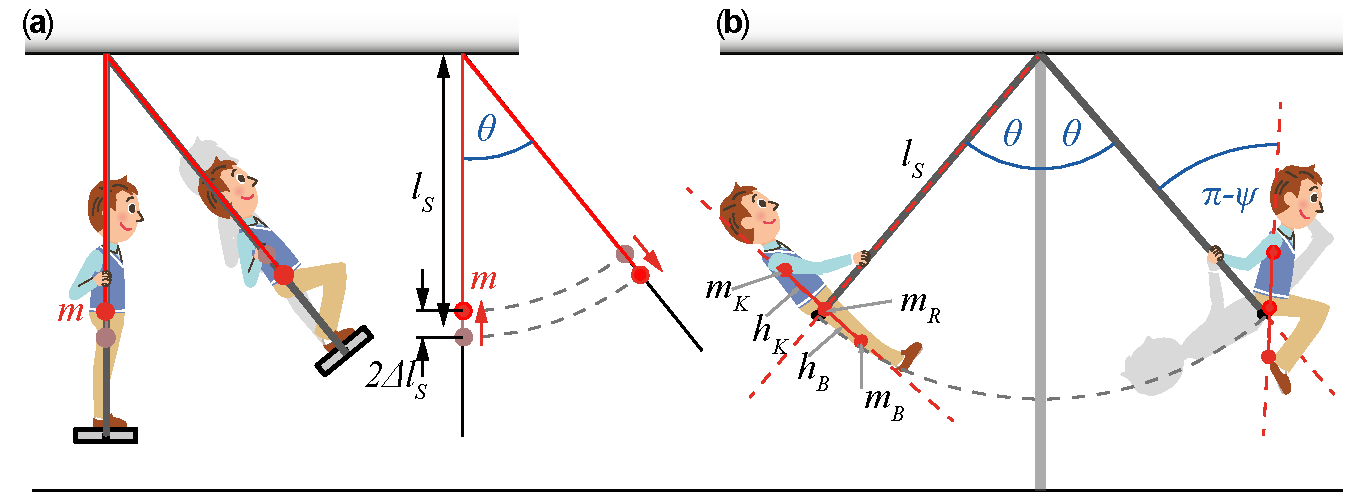
\includegraphics[width=\textwidth]{Schaukel01.pdf}
\caption[Modelle einer Schaukel.]{Modelle einer Schaukel. \fa Einfaches Massepunkt-Modell (Parametrischer Oszillator). \fb Verbessertes Schaukelmodell mit sitzender Person als starrer aber sich parametrisch-dynamisch bewegender K�rper.}
\label{abb:bew_schaukel01a}
\end{figure}

Wir nehmen zur Vereinfachung die Massen der Beine $m_\text{B}$ und des Kopfes $m_\text{K}$ als gleich an.
Die Rumpfmasse wird mit $m_\text{R}$, die Gesamtmasse mit $m_\text{g}$ bezeichnet.
Das \anf{Pumpen} der Schaukel erfolgt durch das Vor- und Zur�cklehnen des gesamten K�rpers mit einem Winkel $\psi$, einem Maximalwinkel $\psi_0$ und einer Frequenz $\omega_\text{A}$ um den Sitzpunkt.
Die Lagrange-Funktion\index{Lagrange-Funktion} ist dann gegeben durch
            \begin{align}
                \mathcal{L} = \frac{1}{2}\,J_1\,\dot{\theta}^2+\frac{1}{2}\,J_2\,\lk\dot{\theta}+\dot{\psi}\rk^2+m_\text{g}\,l_\text{S}\,g\,\cos\theta \,. \label{eq:bew_schaukel11}
            \end{align}
Mit den Massen und Geometrien von Beinen und Kopf $m_\text{g} = m_\text{R}+m_\text{K}+m_\text{B}$ , $m_\text{g} \approx m_\text{R}+2m_\text{K}$ und $h_\text{B} \approx h_\text{K} ={h}/{2}$ haben wir dann folgende Tr�gheitsmomente:
        \begin{align}
						J_1 &=m_\text{g}\,l_\text{S}^2\,~~ J_2=m_\text{K}\,\lk\frac{h^2}{4}+\frac{h^2}{4}\rk = m_\text{K}\,\frac{h^2}{2} \,. \label{eq:bew_schaukel12}
        \end{align}
Unter Ber�cksichtigung der Ann�herung der K�rperschwingung durch die rheonome Zwangsbedingung $\psi = \psi_0\,\cos\omega_\text{A} t$ ergibt sich die Lagrange-Gleichung zu (vgl.\ \kap{bew_Lagrange_I}, \cite{Ray1964})
        \begin{align}
            \lk J_1+J_2\rk\,\ddot{\theta}+m_\text{g}\,l_\text{S}\,g\,\sin\theta = -J_2\,\ddot{\psi} \,. \label{eq:bew_schaukel13}
        \end{align}
\bzw
        \begin{align}
            \ddot{\theta}+{\omega_0}^2\,\sin\theta = F_\text{A}\,\cos\omega_\text{A} t ~~~\text{mit} ~~~ {\omega_0}^2 = \frac{m_\text{g}\,l_\text{S}\,g}{J_1+J_2} ~~ \text{und} ~~ F_\text{A} = \frac{\psi_0\,{\omega_\text{A}}^2\,J_2}{J_1+J_2} \,, \label{eq:bew_schaukel14}
        \end{align}
was eine Gleichung vom Typ des getriebenen Oszillators ist (vgl. \eqref{eq:bew_pendulum02} in \kap{bew_harmon_oszillator}).
Entgegen vielen Lehrbuchdarstellungen scheinen zumindest sitzende Kinder die Schaukel als getriebenes Pendel und nicht als parametrischen Oszillator zu \anf{betreiben}.
Wir wollen aber sicherheitshalber �berpr�fen, ob dies nicht ein Ergebnis unseres zu vereinfachten Modells ist, und nehmen deshalb nun anstelle von \eqref{eq:bew_schaukel12} an, dass $m_\text{K} \neq m_\text{B}$ und auch dass $h_\text{B} \neq h_\text{K}$.
Der K�rper hat dann quasi ein spezifisches (auf $g$ bezogenes) Drehmoment $M_\text{D}$ bez�glich des Sitzpunktes, in dem wir die Rumpfmasse $m_\text{R}$ lokalisiert annehmen:\footnote{Nach unseres bisherigen Annahmen war dieses Drehmoment 0.}
        \begin{align}
            M_\text{D} = m_\text{B}\,h_\text{B}-m_\text{K}\,h_\text{K}\,. \label{eq:bew_schaukel15} 
        \end{align}
Das Tr�gheitsmoment $J_2$ ver�ndert sich nat�rlich zu
        \begin{align*}
            J_2 = m_\text{B}\,{h_\text{B}}^2+m_\text{K}\,{h_\text{K}}^2 \,,
        \end{align*}
und die Lagrange-Funktion lautet nun
        \begin{align}
				\begin{split}
        \mathcal{L} &= \frac{1}{2}\underbrace{J_1\,\dot{\theta}^2+\frac{1}{2}\,J_2\,\lk \dot{\theta}+\dot{\psi}\rk^2-l_\text{S}\,M_\text{D}\,\dot{\theta}\,\lk \dot{\theta}+\dot{\psi}\rk\,\cos\psi}_{\substack{T}} \\
				            &~~~+ \underbrace{m_\text{g}\,l_\text{S}\,g\,\cos\theta - M_\text{D}\,g\,\cos\lk\theta+\psi\rk}_{\substack{-U}}\,. 
        \end{split} \label{eq:bew_schaukel16}
				\end{align}
Der zus�tzliche Term im Potential $U$ ist leicht aus der Geometrie von \figref{bew_schaukel01}b herzuleiten, den Mischterm in der kinetischen Energie $T$ findet man nach etwas Rechnung  am einfachsten aus den kartesischen Koordinaten der drei angenommenen Massepunkte (Man benutze die Symbolic Math Toolbox von \matlab).
Wiederum unter Beachtung der rheonomen Zwangsbedingung $\psi = \psi_0\,\cos\omega_\text{A} t$ ergibt sich die nun etwas komplexere Lagrange-Gleichung f�r die generalisierte Koordinate $\theta$ zu \cite{Case1990}
  \begin{align}
     \underbrace{\lek J_1+J_2 - 2L\,M_\text{D}\,\cos\psi \rek }_{J_\text{eff}(t)} \ddot{\theta} + \underbrace{\lek 2L\,M_\text{D}\,\dot{\theta}\,\dot{\psi}\,\sin\psi \rek}_{\eta_\text{eff}(t)} + \underbrace{\lek m_\text{g}\,l_\text{S}\,g - M_\text{D}\,g\,\cos\psi \rek}_{{\omega_\text{eff}(t)}^2} \sin\theta \nonumber  \\
      \,= -\underbrace{J_2\,\ddot{\psi} - l_\text{S}\,M_\text{D}\,\sin\psi\,\dot{\psi}^2 + l_\text{S}\,M_\text{D}\,\cos\psi\,\ddot{\psi} + M_\text{D}\,g\,\sin\psi\,\cos\theta}_{F_\text{eff}(t)} 
\,.\label{eq:bew_schaukel17}
   \end{align} 
Offensichtlich ist \eqref{eq:bew_schaukel17} von der Struktur einer Schwingungsgleichung in der Koordinate $\theta$, aber mit zeitlich variablen Koeffizienten f�r das Tr�gheitsmoment $J_\text{eff}(t)$, die modifizierte, parametrische Eigenfrequenz $\omega_\text{eff}(t)$ und einem Treiberterm $F_\text{eff}(t)$ auf der rechten Seite.
F�r kleine Schaukelauslenkungen $\theta$ kann man Gl. \eqref{eq:bew_schaukel17} linearisieren und erh�lt
  \begin{align}
     \underbrace{\lek J_1+J_2 - 2L\,M_\text{D}\,\cos\psi \rek }_{J_\text{eff}(t)} \ddot{\theta} + \underbrace{\lek 2L\,M_\text{D}\,\dot{\psi}\,\sin\psi \rek}_{\eta_\text{eff}(t)} \dot{\theta} + \underbrace{\lek m_\text{g}\,l_\text{S}\,g - M_\text{D}\,g\,\cos\psi \rek}_{{\omega_\text{eff}(t)}^2} \theta \nonumber  \\
      = -\underbrace{J_2\,\ddot{\psi} - l_\text{S}\,M_\text{D}\,\sin\psi\,\dot{\psi}^2 + l_\text{S}\,M_\text{D}\,\cos\psi\,\ddot{\psi} + M_\text{D}\,g\,\sin\psi}_{F_\text{eff}(t)} 
\,.\label{eq:bew_schaukel17a}
   \end{align} 
Bevor wir an die numerische L�sung dieser Gleichungen gehen, wollen wir ihre zugrunde liegende physikalische Struktur besser verstehen. Dazu entwickeln wir f�r $\psi(t) = \psi_0\, \cos(\omega_\text{A} t)$ die Winkelfunktionen $\sin\psi$ und $\cos\psi$ in \eqref{eq:bew_schaukel17a} f�r kleine Winkel um $\psi_0$, wobei wir bei der Entwicklung nur Frequenzen bis $2\omega$ mitnehmen wollen.
Wir erhalten dann nach etwas Algebra (als �bung empfohlen, siehe auch \cite{Case1990}) die modifizierte Schwingungsgleichung  
 \begin{align}
      &\ddot{\theta} + \hat{\eta}\,\dot{\theta}+{\hat{\omega}_0}^2\,\theta = \hat{F}_\text{A}\,\cos\omega_\text{A} t \label{eq:bew_schaukel18}
 \end{align} 
mit folgenden zeitabh�ngigen Termen f�r die Reibung $\hat{\eta}$
und das Quadrat der Frequenz $\hat{\omega}_0$:
 \begin{align*}
    \hat{\eta} &= -\frac{l_\text{S}\,M_\text{D}\,\omega_\text{A}\,{\psi_0}^2}{J_0}\,\sin 2\omega_\text{A} t\, ~~~  {\hat{\omega}_0}^2 = {\omega_0}^2 + \frac{M_\text{D}\,g\,{\psi_0}^2}{4\,J_0}\,\cos 2\omega_\text{A} t \,.
 \end{align*}
Hier haben wir die folgenden Konstanten verwendet:
\begin{align*}
			{\omega_0}^2 &= \frac{M_0}{J_0}\,,~~~M_0 = m_\text{g}\,l_\text{S}\,g-M_\text{D}\,g\,\lk 1-\frac{1}{4}\,{\psi_0}^2\rk\,~~\text{und} \\
			J_0 &= J_1 + J_2 -2\,l_\text{S}\,M_\text{D}\,\lk 1-\frac{1}{4}\,{\psi_0}^2\rk \,.
\end{align*}
Auf der rechten Seite von \eqref{eq:bew_schaukel18} steht ein Anregungsterm mit der Grundfrequenz $\omega$, dessen Anregungsst�rke $F_\text{A}$ wiederum zeitlich moduliert ist,
\begin{align} 
    F_\text{A} &= \frac{\psi_0}{J_0}\lek {\omega_\text{A}}^2\,J_2 + M_\text{D}\,\lk g-{\omega_0}^2\,l_\text{S}\rk\lk 1- \frac{{\psi_0}^2}{8}\rk\rek \,.\label{eq:bew_schaukel18a}
\end{align} 
Wir erkennen aus Gleichung \eqref{eq:bew_schaukel18} sehr sch�n,
dass wir eine Kombination von parametrischer Modifikation der Schwingungsfrequenz $\hat{\omega}_0$ (und einer entsprechenden D�mpfung)
und zeitlich variabler Anregung $F_\text{A}$ haben.\\
Ergibt sich nun vielleicht durch die bessere Modellierung des schwingenden K�rpers doch ein parametrischer Oszillator? 

Wir l�sen \eqref{eq:bew_schaukel17} bis \eqref{eq:bew_schaukel19} numerisch (\mscr{} \mlbewref{Schaukel02.m}) mit den Parametern aus Tabelle \ref{tab:bew_schaukel01} und betrachten die zeitliche Entwicklung der Schaukelamplitude (\figref{bew_schaukel05}).
Deutlich ist zu erkennen, dass im Bereich geringer Auslenkungen, also zu Beginn des Schaukelns,
alle drei Rechnungen gut �bereinstimmen und das Verhalten eines getriebenen Pendels vorliegt.
Bei gr��eren Zeiten \bzw Amplituden weichen die Ergebnisse voneinander ab.
Die numerischen Rechnungen f�r die vollst�ndige Lagrange-Gleichung ergeben eine Begrenzung und sogar ein Abnehmen der Amplitude, die Reihenentwicklung zeigt dagegen ein ungest�rtes, nun auch exponentielles Anwachsen, womit wir aber den G�ltigkeitsbereich der N�herung verlassen.
Es bleibt also festzuhalten, dass das Aufschaukeln im wesentlichen der Charakteristik eines getriebenen Oszillators folgt.
Die D�mpfung \bzw Begrenzung der Schwingung resultiert aus der Tatsache, dass die Anregung mit der K�rperschwingungsfrequenz $\omega_\text{A}$ (die in Betrag und Phase in unseren Rechnungen festgehalten wurde) mit der Zeit aus der Phase der Schaukelschwingung mit der Frequenz $\omega_\text{eff}$ l�uft und damit die Schaukelschwingung d�mpft. In der Realit�t passt der Schaukelnde die Phase und Frequenz der K�rperschwingung intuitiv laufend der momentanen Eigenfrequenz der Schaukel an.

Soweit die Rechnungen. Wie kann man aber das Verhalten anschaulich verstehen?
Wir kommen noch einmal auf \eqref{eq:bew_schaukel11} zur�ck und berechnen die Zeitableitung des generalisierten Impulses, die gegeben ist durch 
        \begin{align}
            \dot{p}_\theta = \frac{\D}{\D t}\frac{\d \mathcal{L} }{\d  \dot{\theta}} = J_1\,\ddot{\theta} + J_2\,\lk \ddot{\theta}+\ddot{\psi}\rk = -m_\text{g}\,l_\text{S}\,g\,\sin\theta\,.\label{eq:bew_schaukel19}
        \end{align}
Dieser generalisierte Impuls ist zugleich der Drehimpuls bez�glich der Aufh�ngung.
Er ist offensichtlich wegen des rechten Terms in \eqref{eq:bew_schaukel19} nicht erhalten. Aber selbst wenn $\dot{p}_\theta = 0$ w�re, k�nnte zwischen den beiden Termen in \eqref{eq:bew_schaukel19} ein Drehimpulstransfer stattfinden.
Genau dieser ist zu Beginn des Schaukelns f�r die Dynamik verantwortlich.%
\footnote{Wir wollen noch erg�nzen, dass ein gewisser parametrischer Effekt durch das typische Anziehen der Beine beim Durchgang durch den tiefsten Punkt zu verzeichnen ist, den wir in unseren Rechnungen vernachl�ssigt haben. Ferner ist der Winkel des Zur�cklehnens gegen�ber der aufrechten Haltung �blicherweise merklich gr��er als der des Vorlehnens.}
        \begin{table}[h!]
          \centering
				\begin{tabular}{ l C{2cm} C{2.0cm} C{2.0cm} }
\hline
\rule{0pt}{2pt} & &  \\
              & Kind & Erwachsener\\
\rule{0pt}{2pt} & &  \\
\hline
\rule{0pt}{2pt} & & \\
              $l_\text{S}$  & $\SI{3}{\metre}$ & $\SI{4}{\metre}$ \\
              $m_\text{g}$  & $\SI{50}{\kilogram}$ & $\SI{100}{\kilogram}$ \\
              $h_\text{K}$  & $\SI{0.3}{\metre}$ & $\SI{0.55}{\metre}$ \\
              $h_\text{B}$  & $\SI{0.4}{\metre}$ & $\SI{0.75}{\metre}$ \\
              $m_\text{K}$  & $\SI{15}{\kilogram}$ & $\SI{40}{\kilogram}$ \\
              $m_\text{B}$  & $\SI{15}{\kilogram}$ & $\SI{30}{\kilogram}$ \\
              $m_\text{R}$  & $\SI{20}{\kilogram}$ & $\SI{30}{\kilogram}$ \\
\rule{0pt}{2pt} & & \\
            \end{tabular}
            \caption[Parameter der Schaukel.]{Parameter der Schaukel.}
            \label{tab:bew_schaukel01}
        \end{table}
\begin{figure}
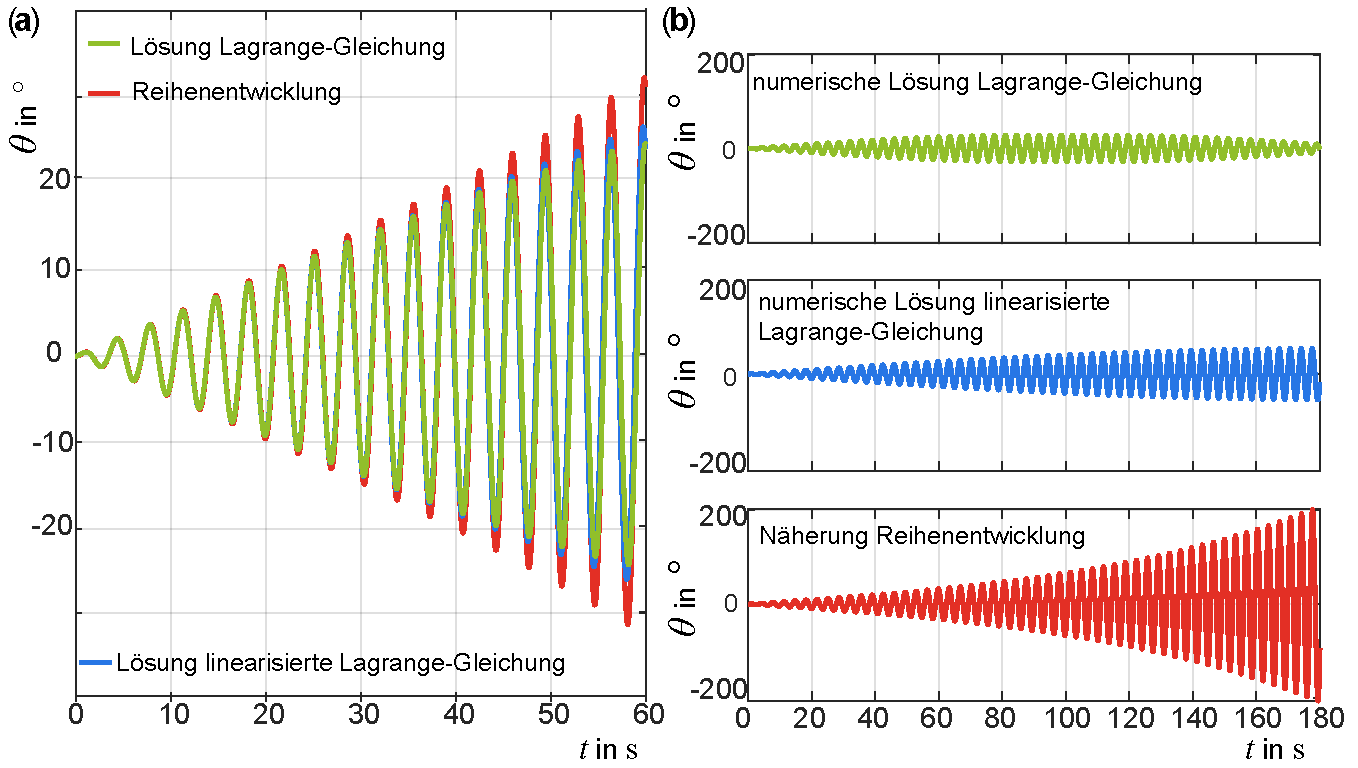
\includegraphics[width=\textwidth]{Schaukel05.pdf}
\caption[Dynamik einer Schaukel als getriebener Oszillator.]{L�sung der Bewegungsgleichung f�r das Modell einer Schaukel als ein getriebener Oszillator f�r \fa Anfangsphase (Kind) und \b l�ngere Zeiten (Erwachsener). Parameter entsprechend \figref{bew_schaukel01} und Tab. \ref{tab:bew_schaukel01}.} 
\label{abb:bew_schaukel05}
\end{figure}

In \probref{bew_schaukelII} schauen wir uns noch die Situation einer im Stehen schaukelnden Person an (siehe auch \cite{Case1996}).
Das Problem kann v�llig analog wie im Fall der sitzenden schaukelnden Person behandelt werden und ergibt als L�sung wieder einen getriebenen Oszillator mit parametrischen Elementen. Noch einen Hinweis zum Schluss: Falls man mal eine Person auf einer Schaukel sieht, die versucht, die Schaukel durch reine parametrische Oszillation, d.h. durch Heben und Senken des K�rpers anzuregen, dann kann man ziemlich sicher sein, dass es sich um einen (theoretischen) Physiker handelt. 


\subsection{Fallende starre K�rper und die rutschende Leiter} \label{kap:bew_fallendeKoerper}

Die einfachen Experimente von fallenden St�ben (und anderen K�rpern wie \zb einem Smartphone)
oder das einer rutschenden Leiter erlauben einige sch�ne Anwendungen
der Physik des starren K�rpers und dar�ber hinaus auch unter Nutzung
von Videokamera und Beschleunigungssensor des Smartphones die einfache
experimentelle �berpr�fung der theoretischen Betrachtungen
und numerischen Rechnungen \cite{Cross2006,Oliveira2016,Kaps2020}.
Sie ergeben dar�ber hinaus, so einfach sie auf den ersten Blick erscheinen, tiefe Einblicke in das Zusammenspiel von Drehmomenten, Reibungskr�ften und tempor�ren Zwangsbedingungen. 


\subsubsection{Fall eines Stabes} \label{kap:bew_fallenderStab}

	Wir beginnen mit dem Umfallen eines urspr�nglich fast senkrecht stehenden Stabes
        ($\theta_0$ betrage einige Grade).
        Wir betrachten dazu \figref{bew_fallingrod01}.
        Der Stab befinde sich auf einer Oberfl�che mit dem Reibungskoeffizienten $\mu$.
        Es wirken neben der Gewichtskraft am Fu�punkt des Stabes
        die Horizontalkraft $F_\text{H}$ und dazu senkrecht die Normalkraft $F_\text{N}$.
        Offensichtlich wird die Reibung einen gro�en Einfluss auf die Bewegung haben.
        Bei einem reibungsfreien Tisch w�rde der Stab einfach wegrutschen
        und der Schwerpunkt sich senkrecht nach unten bewegen.

\begin{figure}
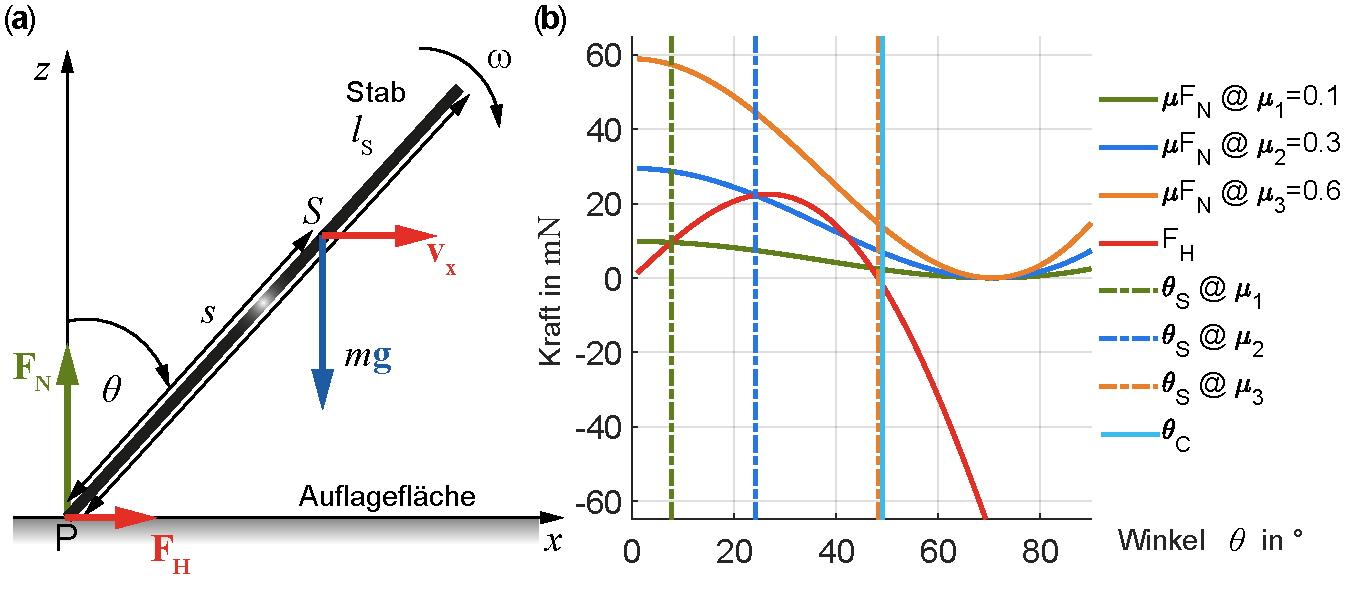
\includegraphics[width=\textwidth]{FallingRod01.pdf}%
\caption[Geometrie und Kr�fte beim umfallenden Stab.]{Geometrie und Kr�fte beim umfallenden Stab. \fa Geometrie und \fb wirkende Kr�fte beim umfallenden Stab. Wenn $F_\text{H} = \mu\,F_\text{N}$ wird, beginnt der Stab bei $\theta_\text{S}$ (f�r $\mu_1$ und $\mu_2$) zu rutschen (gleiten), davor ist der Fu�punkt auf der Unterlage feststehend. F�r das  gr��ere $\mu_3$ beginnt die Gleitphase des Stabes bei $\theta_\text{C}$.}
\label{abb:bew_fallingrod01}
\end{figure}

    Ferner sei $m$ die Masse des Stabes, $\dot{x} = v_\text{x}$ und $\dot{z} = v_\text{z}$ dessen Schwerpunktsgeschwindigkeit in $x$- \bzw $z$-Richtung, $s$ der Abstand des Schwerpunktes vom Fu�punkt am Boden und $J_\text{S}$ das Tr�gheitsmoment bezogen auf den Schwerpunkt.
    Dann gelten die folgenden Bewegungsgleichungen  f�r die generalisierten Koordinaten $x$, $y$, $\theta$:
    \begin{align}
        F_\text{R} &= m\,\ddot{x}\,, \label{eq:bew_fallingrod01a}\\
        F_\text{N} &= m\,\lk \ddot{z} + g \rk\,,\label{eq:bew_fallingrod01b}\\
        M_\text{P} &= F_\text{N}\,s\,\sin\theta - F_\text{H}\,s\,\cos\theta = J_\text{S}\,\ddot{\theta}\,. \label{eq:bew_fallingrod01c}
    \end{align}
Als Anfangsbedingung wollen wir $\dot{z}\lk 0 \rk = v_\text{z}\lk 0\rk = 0$ und $\dot{x}\lk 0 \rk = v_\text{x}\lk 0\rk = 0$,\\ $\dot{\theta}\lk 0\rk = \dot{\theta}_0 = 0$, sowie $\theta\lk 0\rk = \theta_0 > 0$ annehmen.\\
Wir beschreiben zun�chst den Bewegungsablauf genauer, eine Beobachtung desselben ist mit einer Hochgeschwindigkeitsvideoaufnahme mit dem Smartphone leicht zu realisieren:
\begin{enumerate}
    \item Zu Beginn wird der Stab einfach umfallen, das hei�t, $\theta\,, \,\dot{\theta}$ werden mit fortlaufender Zeit gr��er und das untere Fu�ende bleibt ortsfest, solange $F_\text{H} < \mu\,F_\text{N}$. \\
	Wir beschreiben diesen Teil der Bewegung als reine Rotation um den Punkt $P$,
        sodass $\dot{x} = s\,\omega\,\cos\theta$ und $\dot{z} = -s\,\omega\sin\theta$
        und erhalten mit $\dot{\theta} = \omega$ und \eqref{eq:bew_fallingrod01b}
    \begin{align}
      F_\text{H} &= m\,s\,\lk \cos\theta\,\dot{\omega} - \sin\theta\,\omega^2\rk \text{und} \label{eq:bew_fallingrod02}\\
      F_\text{N} &= m\,g -m\,s\,\lk \sin\theta\,\dot{\omega} + \cos\theta\,\omega^2\rk \,. \label{eq:bew_fallingrod03}
    \end{align}
	Wir setzen \eqref{eq:bew_fallingrod02} und \eqref{eq:bew_fallingrod03} in \eqref{eq:bew_fallingrod01c} ein und erhalten mit
	\begin{align}
		\dot{\omega} = \ddot{\theta} = {\omega_0}^2\,\sin\theta ~~\text{und}~~ {\omega_0}^2 = \lk {m\,g\,s}\rk/J_\text{P}  \label{eq:bew_fallingrod04}
	\end{align}
	eine bemerkenswert einfache Gleichung f�r $\theta$ mit $J_\text{P} = J_\text{S} + m\,s^2$ als Tr�gheitsmoment bez�glich des Fu�punktes.
        Letzteres gilt f�r homogene St�be $J_\text{P} = m\,l_\text{S}{}^2/3$ mit $l_\text{S}=2s$.
        Wir weisen nochmals darauf hin, dass \eqref{eq:bew_fallingrod04} nur gilt,
        solange der Punkt $P$ fest bleibt.
        Dann kann man \eqref{eq:bew_fallingrod04} integrieren und erh�lt,
        wie man durch Differenzieren leicht nachrechnet,
    \begin{align}
        \omega^2 = 2\,{\omega_0}^2\,\lk\cos\theta_0-\cos\theta\rk \,,\label{eq:bew_fallingrod05}
    \end{align}
sodass sich f�r die Kr�fte $F_\text{H}, \, F_\text{N}$ als Funktion des Winkels $\theta$ mit \eqref{eq:bew_fallingrod02} und \eqref{eq:bew_fallingrod03} ergibt: 
    \begin{align}
    \begin{split}
        F_\text{H} &= m\,s\,{\omega_0}^2\,\sin\theta\,\lk 3\cos\theta-2\cos\theta_0\rk \,, \\
        F_\text{N} &= m\,g - m\,s\,{\omega_0}^2\,\lk 1+2\cos\theta\,\cos\theta_0 - 3\cos^2\theta\rk \,. \label{eq:bew_fallingrod06}
    \end{split}
    \end{align}
		Die Kr�fte $F_\text{H}, \, F_\text{N}$ sind in \figref{bew_fallingrod01}b (siehe auch \mscr{} \mlbewref{FallenderStab01.m}) dargestellt.
                Man erkennt aus \eqref{eq:bew_fallingrod06} und der Abbildung, dass die Horizontalkraft $F_\text{H}$ sich ab einem bestimmten Winkel verringert und dann das Vorzeichen wechselt.%
                \footnote{Physikalisch kann man das als Ergebnis der Horizontalkomponente der wirkenden Zentripetalkraft des drehenden Stabes verstehen.} 
    \item Bei einem bestimmten Winkel $\theta_\text{S}$
      abh�ngig von der Oberfl�chenreibung $\mu$ des Tisches
      wird der untere Fu�punkt des Stabes ins Rutschen/Gleiten kommen,
      da dann $F_\text{H}(\theta_\text{S}) = \mu\, F_\text{N}(\theta_\text{S})$ gilt.
      Mit \eqref{eq:bew_fallingrod06} berechnet sich der Winkel $\theta_\text{S}$ aus
      \footnote{Eigentlich m�sste man bei der Behandlung der Reibung
      zwischen Haftreibung $\mu_\text{H}$ und Gleitreibung $\mu_\text{G}$ unterscheiden.
      Wir empfehlen dem Leser, das f�r die numerische Berechnung zu tun,
      in der einfach eine entsprechende Fallunterscheidung programmiert werden kann.}
    \begin{align}
	\begin{split}
        \mu &= \frac{m\,s\,{\omega_0}^2\,\sin\theta_\text{S}\,\lk 3\cos\theta_\text{S}-2\cos\theta_0\rk }{m\,g - m\,s\,{\omega_0}^2\,\lk 1+2\theta_\text{S}\,\cos\theta_0 - 3\cos^2\theta_\text{S}\rk }\, \\
				&\text{\bzw f�r einen homogenen Stab} \\
				\mu &= \frac{9\sin\theta_\text{S}\,\cos\theta-6\cos\theta_0\,\sin\theta_\text{S}}{1+9\cos^2\theta_\text{S}-6\cos\theta_0\,\cos\theta_\text{S}} \,.
				\label{eq:bew_fallingrod07}
	\end{split}
    \end{align}
	In \figref{bew_fallingrod01}b sind f�r die zwei Reibungskoeffzienten
        $\mu_1$ und $\mu_2$ die entsprechenden Winkel $\theta_\text{S}(\mu)$
        eingezeichnet.
        Man erkennt sehr sch�n, dass dort tats�chlich
        $F_\text{H}(\theta_\text{S}) = \mu\, F_\text{N}(\theta_\text{S})$ gilt.
	\item In \figref{bew_fallingrod01}b ebenfalls eingezeichnet
          ist der kritische Winkel $\theta_\text{C}$,
          bei welchem die Horizontalkraft $F_\text{H} = 0$ ist.
          Bei diesem Winkel beginnt unabh�ngig vom Reibungskoeffizienten $\mu$
          der Stab am Fu�punkt auf jeden Fall zu gleiten.
          Der Winkel $\theta_\text{C}$ berechnet sich f�r einen homogenen Stab zu
    \begin{align}
	\theta_\text{C} =\arccos\lk \frac{2}{3} \cos\theta_0 \rk \,. 	\label{eq:bew_fallingrod08}
    \end{align}
	\item Es gibt also zwei m�gliche Einsetzpunkte des Gleitens:
          $\theta_\text{S}$ und $\theta_\text{C}$.
          Beim Einsetzen bei $\theta_\text{S}$ wird das untere Ende des Stabes
          zu kleineren $x$-Werten rutschen, beim Einsetzen bei $\theta_\text{C}$ umgekehrt. 
\end{enumerate}
Wir haben damit nun alle Informationen, um die Bewegung analytisch zu beschreiben
und auch numerisch zu berechnen.
Wir unterteilen dazu die Bewegung in zwei Phasen,
die einfache Rotation um den Punkt $P$ und die gekoppelte Rotation
mit der horizontalen Bewegung des Fu�punktes.
Wir betrachten zun�chst die reine Rotation um den Punkt $P$.
Hier k�nnen wir einfach die Bewegungsgleichung \eqref{eq:bew_fallingrod04}
numerisch bis $\theta_\text{S}$ \bzw $\theta_\text{C}$ integrieren.
Etwas schwieriger ist die Phase 2.
F�r diese Phase muss man in \eqref{eq:bew_fallingrod02}
$F_\text{R} = \mu\,F_\text{N}$ setzen und erh�lt daraus
mit \eqref{eq:bew_fallingrod01c} und \eqref{eq:bew_fallingrod03}
die folgende Bewegungsgleichung f�r $\ddot{\theta}$: 
    \begin{align}
	\begin{split}
        \ddot{\theta} &= \frac{m\,s\,\lk g-s\,\dot{\theta}^2\,\cos\theta\rk\lk\sin\theta-\mu\,\cos\theta\rk}{J_\text{S} + m\,H^2\,\sin\theta\,\lk \sin\theta-\mu\cos\theta\rk} \\
				&\text{\bzw f�r einen homogenen Stab} \\
	\ddot{\theta} &= \frac{\frac{g}{s} - {\dot{\theta}}^2\,\cos\theta}{\sin\theta + C(\theta)} ~~~\text{mit} ~~~ C(\theta) = \lk 3 \sin\theta - 3 \mu \cos\theta \rk^{-1}\,. \label{eq:bew_fallingrod08a}
	\end{split}
    \end{align}
Man beachte, dass je nach der Art des Einsetzens des Gleitens,
\dh je nachdem, ob $F_\text{H}$ zum Zeitpunkt des Einsetzens des Rutschens
bereits das Vorzeichen gewechselt hat, $\mu>0$ (f�r $\theta_\text{S}$)
\bzw $\mu<0$ (f�r $\theta_\text{C}$) gesetzt werden muss.
In der numerischen Rechnung im \mscr{} \mlbewref{FallenderStab02.m}
wird das entsprechend ber�cksichtigt.
Zus�tzlich muss noch die Bewegung des Fu�punktes $x_\text{P}$ berechnet werden.
F�r den homogenen Stab ergibt sich aus den Bewegungsgleichungen
\eqref{eq:bew_fallingrod01a}--\eqref{eq:bew_fallingrod01c} \cite{Oliveira2016}:
    \begin{align}
        \ddot{x}_\text{P} &= s \, \dot{\theta}^2 \sin\theta - s\, \ddot{\theta} \lk \cos\theta - \mu\, C(\theta) \rk\,. \label{eq:bew_fallingrod08b}
    \end{align}

\begin{figure}
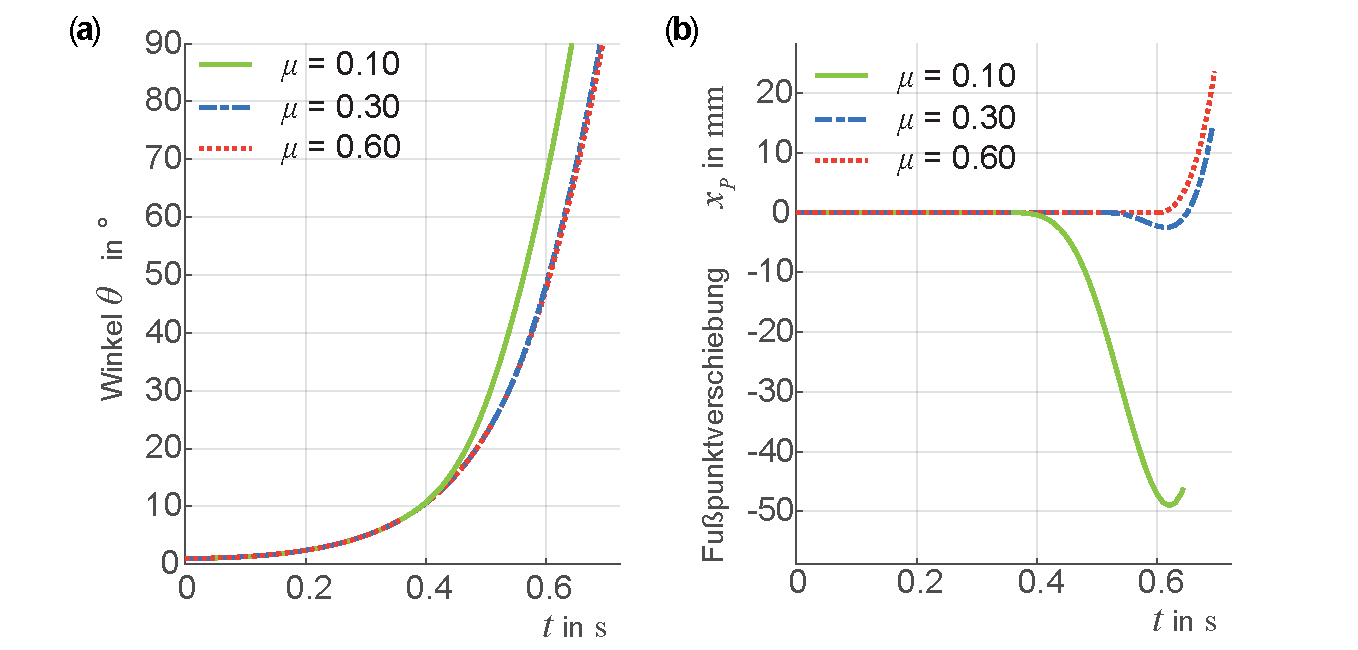
\includegraphics[width=\textwidth]{FallingRod02.pdf}%
\caption[Dynamik eines umfallenden Stabes.]{Dynamik eines umfallenden Stabes. \fa Dargestellt ist die zeitliche Entwicklung des Winkels $\theta(t)$ f�r verschiedene Reibungen. \fb $x$-Position des Stabendes als Funktion der Zeit f�r verschiedene Reibungskoeffizienten.} \label{abb:bew_fallingrod02}
\end{figure}

In \figref{bew_fallingrod02}a haben wir den Fallwinkel $\theta$
als Funktion der Zeit f�r verschiedene Reibungskoeffizienten berechnet.
Man erkennt eine relativ geringe Abh�ngigkeit der Fallzeit vom Reibungskoeffizienten.
\figref{bew_fallingrod02}b zeigt den Fu�punkt $x_\text{P}$ des Stabes
als Funktion der Zeit, wiederum f�r verschiedene Reibungskoeffizienten.
Man erkennt, dass f�r eine rauere Oberfl�che (ein gr��eres $\mu$)
das Stabende sich in Neigungsrichtung ($x >0$) bewegt,
w�hrend f�r eine glattere Oberfl�che, wie nicht anders zu erwarten war,
das Stabende sich (zun�chst) in entgegengesetzte Richtung bewegt, also wegrutscht.
Dieses interessante Verhalten des Stabes, insbesondere auch
das R�ckw�rts- und anschlie�ende Vorw�rtsgleiten bei geringen $\mu$,
kann durch das Zusammenspiel der Horizontalkomponente der Linearbeschleunigung
und der Zentripetalkraft ($\propto \dot{\theta}$)
des drehenden Stabes verstanden werden.
Dem Leser wird empfohlen, mit dem 
\mscr{} \mlbewref{FallenderStab02.m} auch die $\theta_0$-Abh�ngigkeit
und die Wirkung inhomogener Massenverteilungen zu studieren.\\
Zum Schluss sei noch im Zusammenhang mit dem behandelten Problem
auf eine interessante Frage verwiesen:
Kann das Fu�ende des Stabes \anf{abheben}, \dh kann zu irgendeinem Zeitpunkt
w�hrend des Fallens $z_\text{P} > 0$ gelten?%
\footnote{Wir �berlassen dem Leser die (numerische) �berpr�fung.}
Diese Frage ist �brigens eng verwandt mit der Frage
nach der maximalen Gehgeschwindigkeit des Menschen:
Bis zu welcher Bewegungsgeschwindigkeit $v$ bleibt der K�rper
mit mindestens einem Fu� auf dem Boden?
Da der Schwerpunkt des K�rpers eines Menschen ($s\approx \SI{1}{\metre}$)
um den Fu�auflagepunkt \anf{rotiert}, gilt f�r die Normalkraft
    \[F_\text{N} \approx m\,g - m\,v^2/s\,,\]
und damit $F_\text{N}>0$ bleibt, darf die Geschwindigkeit
nicht gr��er als $v_\text{max} =\sqrt{g\,s} \approx \SI{3}{\metre\per\s}$ werden,
was gut mit der Erfahrung �bereinstimmt.
Beim sportlichen Gehen erreichen die schnellsten M�nner
Geschwindigkeiten von $v_\text{max} =\sqrt{g\,s} \approx 4.5 \text{ bis } \SI{5}{\metre\per\s}$,
was nur durch eine spezielle Geher-Technik erreicht wird.

\subsubsection{Vergleich umfallender St�be mit verschiedenen Masseverteilungen}

Bevor wir uns dem verwandten Problem der rutschenden Leiter zuwenden,
wollen wir uns noch einen \glqq Wettbewerb\grqq{} �berlegen
und 3 umfallende St�be der L�nge $l_\text{S}$ mit unterschiedlicher Masseverteilung vergleichen \cite{Shan2020}.
\begin{enumerate}
    \item [a)] homogener Stab der Gesamtmasse $m+m_\text{T}$
    \item [b)] homogener Stab der Masse $m$ mit Gewicht $m_\text{T}$ am Ende des Stabes
    \item [c)] homogener Stab der Masse $m$ mit 2 Gewichten $m_\text{T}/2$ an den Positionen $l_\text{S}/3$ und $2 l_\text{S}/3$
\end{enumerate}
Welcher Stab erreicht als erster die Horizontale? Wir wollen uns die Rechnung etwas vereinfachen und nehmen das Fu�ende als festgehalten an,
was $\mu \rightarrow\infty$ entspricht. Bei festem Drehpunkt k�nnen wir die Bewegungsgleichungen entsprechend \eqref{eq:bew_fallingrod04} aufschreiben und folgende Tr�gheitsmomente und Schwerpunktlagen berechnen (dabei sei $m_\text{T}/m = \gamma = 5$ angenommen):
    \begin{align}
        J_\text{a} &= \frac{1}{3}\,\lk m+m_\text{T}\rk\,l_\text{S}^2 = 2m\,l_\text{S}^2
        &r_\text{s,a} &= \frac{l_\text{S}}{2} \,,\notag\\
        J_\text{b} &=\frac{1}{3}\,m\,l_\text{S}^2 + m_\text{T}\,l_\text{S}^2 = \frac{16}{3}\,m\,l_\text{S}^2
        &r_\text{s,b} &= \frac{11}{12}\,l_\text{S}\,,
    \label{eq:bew_fallingrod09}
        \\
        J_\text{c} &=\frac{1}{3}\,m\,l_\text{S}^2 + \frac{m_\text{T}}{2}\,\lek\frac{l_\text{S}^2}{9} + \frac{4L^2}{9}\rek = \frac{11}{18}\,m\,l_\text{S}^2
        &r_\text{s,c} &=  \frac{l_\text{S}}{2} = r_\text{s,a}\,. \notag
    \end{align}
Die Winkelbeschleunigungen $\ddot{\theta}_\text{i}$ ergeben sich mit den Drehmomenten $M_\text{D,i}$ zu
    \begin{align}
      \ddot{\theta}_i = \frac{M_{\text{D},i}}{J_i} = \frac{\lk m+m_\text{T}\rk\,g\,r_{\text{s},i}\,\sin\theta}{J_i} ~~~~~i = \text{a,b,c} \label{eq:bew_fallingrod10}
    \end{align}
\bzw im einzelnen Fall durch
\begin{align*}
			\ddot{\theta}_\text{a} &= \frac{3}{2}\,g\,\sin\theta / l_\text{S}\,,~
			~~~\ddot{\theta}_\text{b} = \frac{33}{32}\,g\,\sin\theta / l_\text{S}\,,~
			~~~\ddot{\theta}_\text{c} = \frac{54}{11}\,g\,\sin\theta / l_\text{S}\,.
\end{align*}
\begin{figure}
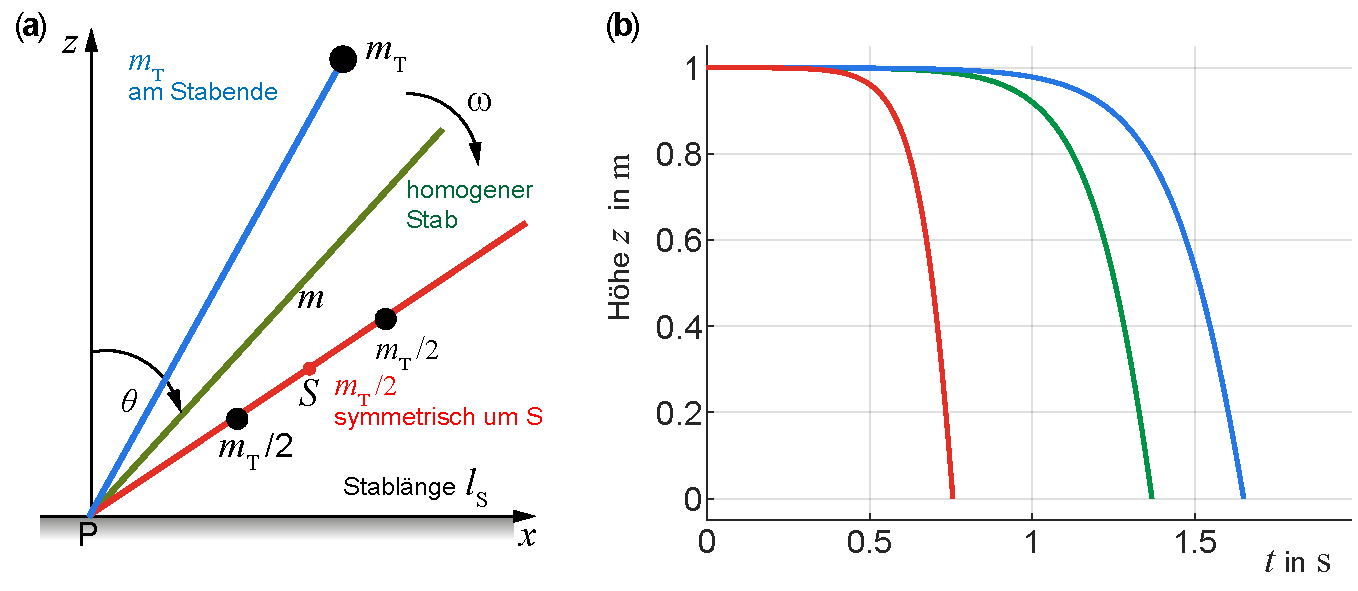
\includegraphics[width=\textwidth]{FallingRod03.pdf}%
\caption[Dynamik umfallender St�be verschiedener Massenverteilungen.]{Dynamik umfallender St�be verschiedener Massenverteilungen.} \label{abb:bew_fallingrod03}
\end{figure}
Die Integration der Bewegungsgleichung ist in \figref{bew_fallingrod03} dargestellt.
Wie man sieht, f�llt der Stab c am schnellsten fallende Stab.
Die unterschiedlichen Fallzeiten haben ihre Ursache darin,
dass in \eqref{eq:bew_fallingrod09} und \eqref{eq:bew_fallingrod10}
sowohl das Tr�gheitsmoment als auch das wirkende Drehmoment
von der Massenverteilung entlang des Stabes abh�ngig sind. \\

\subsubsection{Umfallende Leiter} \label{kap:bew_fallendeLeiter}

\begin{figure}
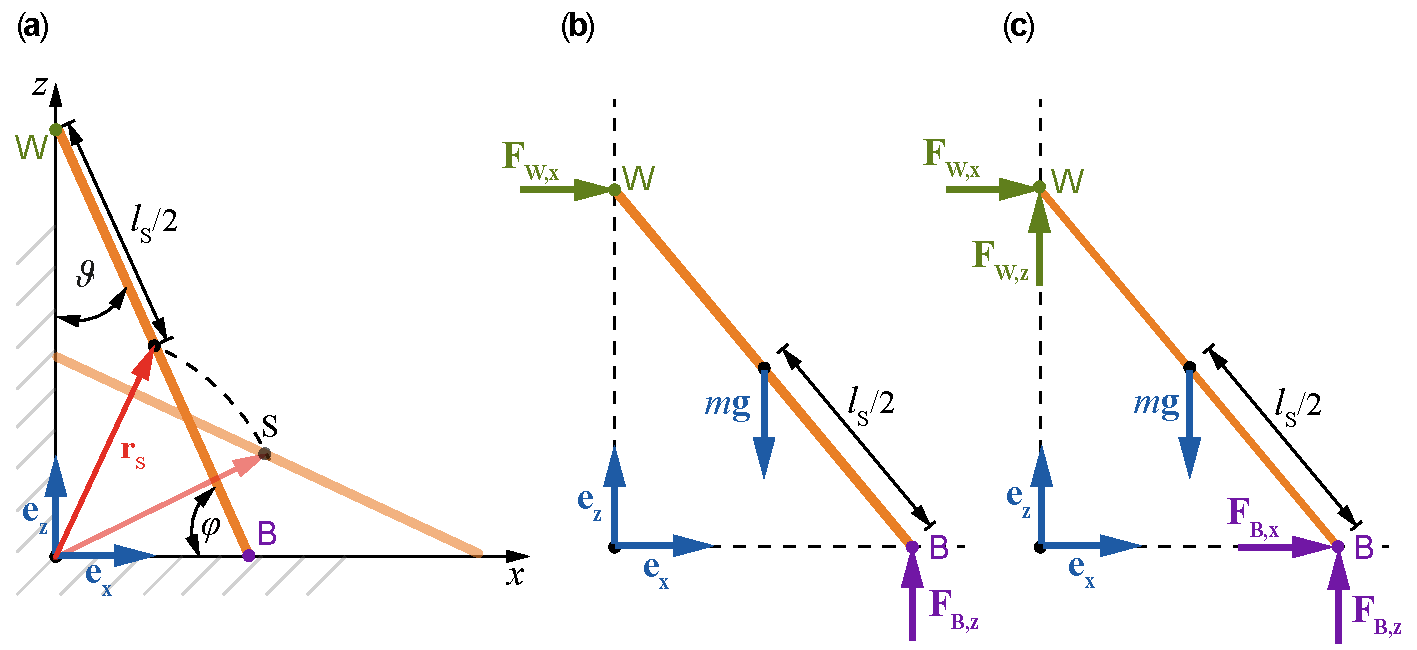
\includegraphics[width=\textwidth]{Ladder01.pdf}%
\caption[Geometrie und Kr�fte der umfallenden Leiter.]{Geometrie und Kr�fte der umfallenden Leiter. \fa Geometrie, \fb Normalkr�fte und \fc Normal- und Reibungskr�fte.} \label{abb:bew_ladder01}
\end{figure}

Eines der scheinbar einfachen Probleme der Mechanik ist das der \anf{umfallenden} \bzw \anf{wegrutschenden} Leiter.
So einfach es auf den ersten Blick erscheint,
so �berraschend sind doch die dabei zu ber�cksichtigenden physikalischen Effekte,
sodass es bis heute \zt einander widersprechende Ver�ffentlichungen
zu diesem Problem gibt, siehe dazu \cite{Oliveira2015, Glane2019, Ghorashi2019} und dort angegebene Referenzen.

Wir betrachten \figref{bew_ladder01}\,a, nehmen die Leiter als homogen an und stellen zun�chst eine einfache energetische Betrachtung an.

\subparagraph{Energiebetrachtung f�r die fallende Leiter}~

Aus der Abbildung sehen wir, dass der Vektor $\vec r$ vom Ursprung zum Schwerpunkt S
beim Rutschen der Leiter zun�chst eine Kreisbahn beschreibt.
Interessant ist der Punkt \bzw die Richtung von $\vec r$, bei dem die Leiter den Kontakt
zur Wand am Punkt B oder W verliert.
Dies wird bei einem Winkel $\vartheta_S=90\degree - \varphi_S$ passieren, bei dem die $x$-Komponente
der Schwerpunktgeschwindigkeit abnimmt,
\dh die Beschleunigung und damit die Normalkraft am Punkt W negativ werden m�sste.
Das ist aber physikalisch unm�glich, sodass dies der Punkt ist,
ab dem die Leiter sich von der Wand l�st, also richtig \anf{wegrutscht}.

Aus der Energieerhaltung folgt f�r die Schwerpunktskoordinaten ausgedr�ckt �ber den Winkel $\vartheta$
\begin{align}
 \Delta U &= T_{\text{Trans}} + T_{\text{Rot}}\,=\, m\,g\,r(1-\cos\vartheta) = \frac m2\lk\dot x^2+\dot z^2\rk + \frac J2 \dot\vartheta^2\notag\\
  &=\frac m2r^2\dot\vartheta^2 + \frac J2\dot\vartheta^2 = \frac12\lk mr^2+J\rk\dot\vartheta^2\,.
  \label{eq:bew_ladder01}
\end{align}

F�r die homogene Masseverteilung gilt $J=\frac1{12}m l_\text{S}{}^2=\frac13mr^2$.

Wir l�sen \eqref{eq:bew_ladder01} nach $v=r\vartheta$ und erhalten f�r die Horizontalkomponente der Schwerpunktsgeschwindigkeit 
\begin{align}
  v_x &= v\, \sin(90\degree -\vartheta) = \sqrt{\frac{3gr(1-\cos\vartheta)}2}\,\cos\vartheta
	    = \sqrt{\frac{3gr}2}\sqrt{(1-u)u^2}\,.\label{eq:bew_ladder02}
\end{align}

Wir suchen das Maximum von $v_x$
(da ab dort eine Verringerung der Horizontalgeschwindigkeit einsetzen w�rde)
und erhalten
\begin{equation}
  \cos\vartheta_S = \frac23\quad\rightarrow\quad\vartheta_S\approx\SI{48.2}{\degree}\,.
  \label{eq:bew_ladder03}
\end{equation}

Man kann nun noch fragen, bei welchem Winkel $\vartheta_M$ die Leiter am Punkt W
die maximale Normalkraft der Wand erf�hrt, \dh am sichersten an der Wand steht.

Wir bilden
\begin{align}
  F_{N,W} &\propto \frac{\D}{\D\vartheta}v_x\cdot\frac{\D\vartheta}{\D t}\propto\lk\frac12\frac{\cos\vartheta\sin\vartheta}{\sqrt{1-\cos\vartheta}}
  -\sqrt{1-\cos\vartheta}\sin\vartheta\rk\dot\vartheta\notag\\
  &=\dot\vartheta\sin\vartheta\lek\frac{\cos\vartheta-1+2\cos\vartheta}{\sqrt{1-\cos\vartheta}}\rek \propto\sin\vartheta(3\cos\vartheta-2)\cdot\dot\vartheta\,.
  \label{eq:bew_ladder04}
\end{align}
Die Maximalbedingung ergibt
\begin{align*}
  \frac{\partial F_{N,W}}{\partial\vartheta}=0
  &=\cos\vartheta(3\cos\vartheta-2) - 3\sin\vartheta\,\sin\vartheta \\
  %&=3\cos^2\vartheta -2\cos\vartheta - 3\sin^2\vartheta\\
  %&=3\cos^2\vartheta - 2\cos\vartheta - 3 + 3 \cos^2\vartheta\\
  &=6\cos^2\vartheta - 2\cos\vartheta - 3
\end{align*}
und mit $u=\cos\vartheta$
\begin{align}
  u^2-\frac13u-\frac12 &= 0\,~~\rightarrow~~ f_{1,2} = \frac16\pm\sqrt{\frac1{36}+\frac{18}{36}}= \frac16\pm\frac{\sqrt{19}}6\,,
  \label{eq:bew_ladder05}
\end{align}
wir erhalten also $\cos\vartheta_M = \frac16(1+\sqrt{19})$ und mithin $\vartheta_M\approx\SI{26.7}{\degree}$.
Man tut also gut daran, die Leiter etwas steiler als
$\varphi = \SI{90}{\degree}-\vartheta = \SI{60}{\degree}$ zu stellen.

\subparagraph{Dynamische Betrachtung}

Nach diesen eher grunds�tzlichen �berlegungen wollen wir uns nun der Dynamik zuwenden und benutzen dabei vorteilhafterweise den Winkel $\varphi$ als generalisierte Koordinate.

Wir betrachten \figref{bew_ladder01}, wo wir im Fall b)
die Leiter ohne Reibungseinfluss der W�nde betrachten wollen und im Fall c)
mit den Reibungskr�ften von Wand und Boden.
Aus der Zwangsbedingung, dass die Leiter bis zum Abl�sen
in Kontakt zu Wand und Boden ist,
k�nnen wir folgende kinematische Bedingungen als Funktion von $\varphi(t)$ aufschreiben:
\begin{align}
  %\text{Auflagepunkte B,W:}  \notag\\
  \vec x_n &= x_B\,\vec e_x = l_\text{S}\,\cos\varphi\vec e_x\,,~~ \vec z_W = z_W\,t\vec e_z = l_\text{S}\,\sin\varphi\vec e_z\notag\\
  %\text{Schwerpunkt S:} \notag\\ 
  \vec x_S &= \frac{ l_\text{S}}{2}\cos\varphi\vec e_x + \frac{ l_\text{S}}{2} \sin\varphi\vec e_z\,,~~ \dot{\vec x}_S = \frac{ l_\text{S}}{2}\dot\varphi\lk\sin\varphi\vec e_x+\cos\varphi\vec e_z\rk
  \notag\\
  \ddot{\vec x}_S &= \frac{ l_\text{S}}{2}\lek\lk-\sin\varphi\cdot\ddot\varphi-\cos\varphi\dot\varphi^2\rk\vec e_x
  +\lk\cos\varphi\ddot\varphi-\sin\varphi\dot\varphi^2\rk\vec e_z\rek\,.
  \label{eq:bew_ladder06}
\end{align}

Wir schreiben nun die Kr�fte und Drehmomente gem�� \figref{bew_ladder01}b auf:
\begin{align}
\begin{split}
  m\,\ddot{\vec x}_S &= F_{W,x}\,\vec e_x + \lk F_{B,z} - mg\rk\,\vec e_z\,, \\
  J_S\,\ddot\varphi &= -(x_B-x_S)\,F_{B,z} - (z_W-z_S)\,F_{W,x}\,.
\end{split}
  \label{eq:bew_ladder07}
\end{align}

Das Minuszeichen resultiert aus der Tatsache, dass die rutschende Leiter
sich gegen den Uhrzeigersinn \anf{dreht}. Setzen wir \eqref{eq:bew_ladder06} in \eqref{eq:bew_ladder07} ein,
erhalten wir durch Elimination der Wandkr�fte die Bewegungsgleichung f�r $\varphi(t)$
f�r $J_S=\frac1{12}m l_\text{S}{}^2$:
\begin{equation}
  \ddot\varphi(t) = -\frac32\frac{g}{l_\text{S}}\cos\varphi(t)\,.
  \label{eq:bew_ladder08}
\end{equation}

Die Normalkr�fte an Wand und Boden als Funktion des Winkels lauten
\begin{align*}
  F_{B,z} &= -\frac{m l_\text{S}}2\lk\frac{3g}{2 l_\text{S}}\cos^2\varphi+\sin\varphi\,\dot\varphi^2\rk \,+\,m\,g~~~\text{ und}\\
  F_{W,x} &= +\frac{m l_\text{S}}2\cos\varphi\lk\frac{3g}{2 l_\text{S}}\sin\varphi-\dot\varphi^2\rk\,.
\end{align*}

\begin{figure}
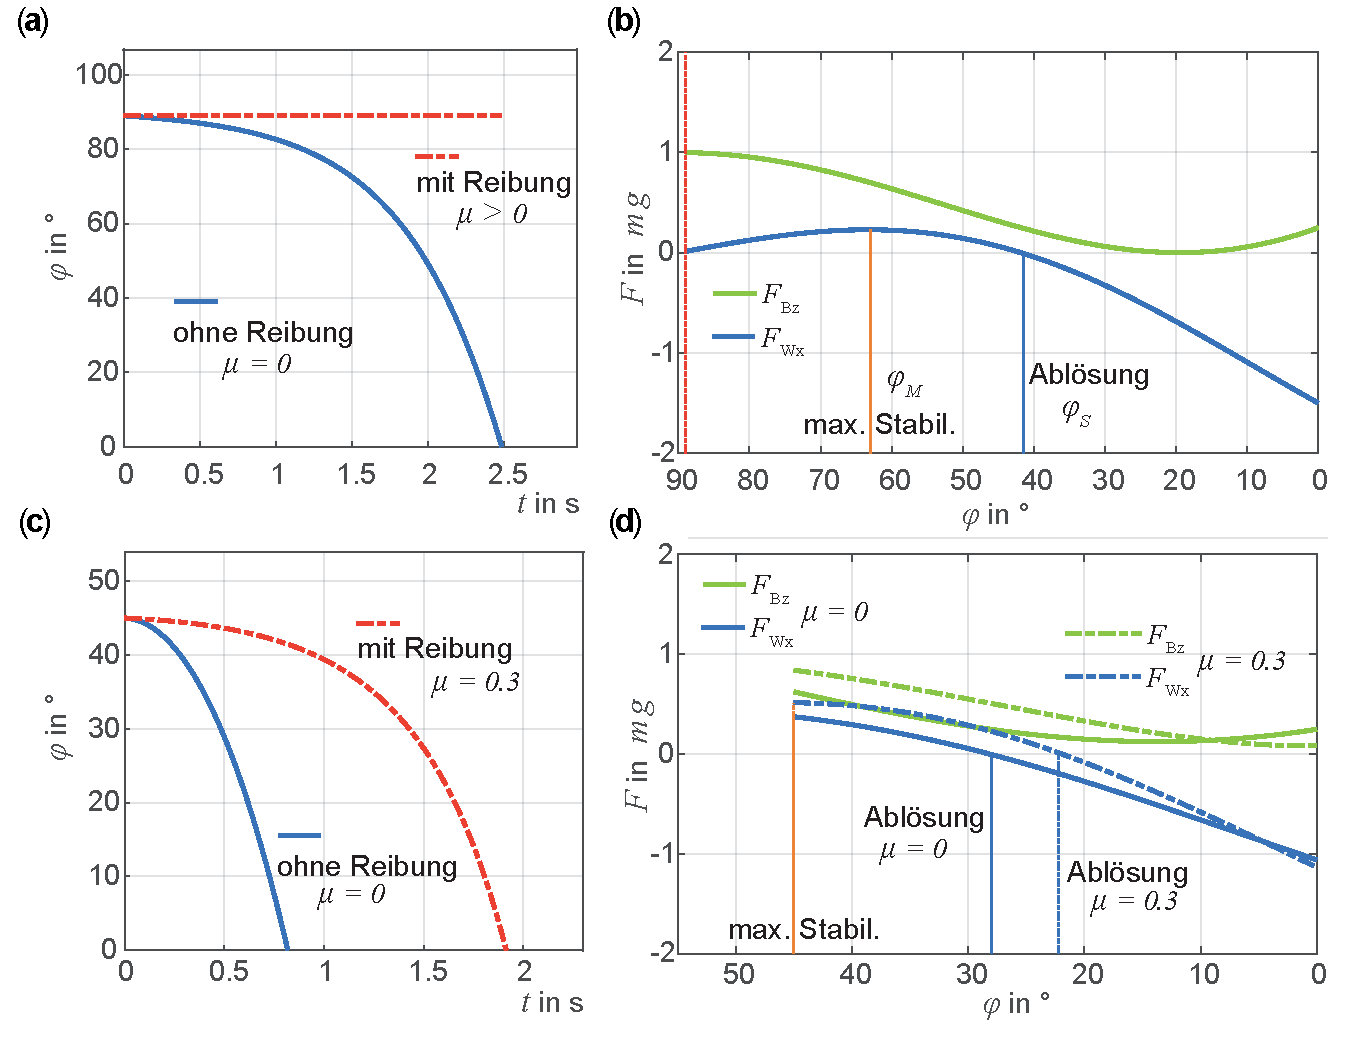
\includegraphics[width=\textwidth]{Ladder02.pdf}
\caption[Dynamik der umfallenden Leiter mit und ohne Reibung.]{Dynamik der umfallenden Leiter mit und ohne Reibung.
\fa Dynamik mit $\vartheta(0) \approx 0 \cong \varphi(0) \approx 90\degree$.
Bei $\mu >0$ rutscht die Leiter nicht weg.
\fb Normalkr�fte an Wand und Boden bei $\vartheta(0) = 0 \equiv \varphi(0) \approx 90\degree$.
Die Abl�sung der Leiter erfolgt im reibungsfreien Fall bei $\varphi_S\approx 42\degree$  \bzw $\vartheta_S\approx 48\degree$,
die maximale Stabilit�t hat die Leiter bei $\varphi_M\approx 63\degree$ \bzw $\vartheta_M\approx 27\degree$.
\fc Dynamik mit Startwinkel der Leiter bei $\varphi(0) = \vartheta(0) = 45\degree$.
Hier rutscht die Leiter auch bei $\mu = 0.3$ weg, aber entsprechend langsamer als im reibungsfreien Fall.
\fd Normalkr�fte an Wand und Boden bei $\varphi(0) \approx 45\degree$.
Die Abl�sung der Leiter im reibungsfreien Fall erfolgt bei $\varphi_S\approx 28\degree$, bei einem Reibungskoeffizienten von $\mu = 0.3$ erst bei $\varphi_S\approx 22.5\degree$
(Siehe \mscr{} \mlbewref{FallendeLeiter.m}).} \label{abb:bew_ladder02}
\end{figure}

In \figref{bew_ladder02} haben wir die zeitliche Entwicklung von $\varphi(t)$
und die Kr�fte $F_{B,z},\, F_{W,x}$ dargestellt. Die Rechnungen best�tigen unser �ber den Energieerhaltungssatz erhaltenes Ergebnis
\eqref{eq:bew_ladder05}.

Wir k�nnen uns jetzt noch fragen, welchen Einfluss die Reibung an Wand und Boden
auf die Dynamik der fallenden Leiter hat.
Dazu m�ssen wir \eqref{eq:bew_ladder07} um die Reibungskr�fte erweitern und erhalten
\begin{align}
\begin{split}
  m\,\ddot{\vec{x}}_S &= (F_{B,x}+F_{W,x})\,\vec e_x + (F_{B,z}+F_{W,z}-mg)\,\vec e_z\,, \\
  J_S\,\ddot\varphi &= -(z_B-z_S)\,F_{B,x} + (x_B-x_S)\,F_{B,z} \\
  &= -(z_W-z_S)\,F_{W,x} + (x_W-x_S)\,F_{W,z}\,.
\end{split}
  \label{eq:bew_ladder09}
\end{align}
Hierin sind jetzt $F_{B,x}$ und $F_{W,z}$
die Komponenten der Reibungskr�fte, die wir als Gleitreibungskr�fte annehmen k�nnen,
sodass wir mit der Vereinfachung $\mu_W = \mu_B = \mu$ schreiben k�nnen:
\begin{align}
\begin{split}
  F_{B,x} &= -\sgn(\vec v_B\cdot\vec e_x)\,\mu\,|F_{B,z}| = \sgn(\dot\varphi)\,\mu\,|F_{B,z}| \; , \\
  F_{W,z} &= -\sgn(\vec v_W\cdot\vec e_z)\,\mu\,|F_{W,x}| = -\sgn(\dot\varphi)\,\mu\,|F_{W,x}|\;.
\end{split}
 \label{eq:bew_ladder10}
\end{align}

Die Reibungskr�fte $F_{B,x}$ \bzw $F_{W,z}$ an Boden und Wand sind hierbei �ber die 
an der Wand \bzw am Boden wirkenden Normalkr�fte definiert.
Wegen der Richtungsabh�ngigkeit haben wir vorteilhaft die $\sgn$-Funktion%
\footnote{In \matlab{} und auch vielen B�chern wird die $\sgn$-Funktion mit $\mathrm{sign}$ bezeichnet.} benutzt
\cite{Glane2019}:
\begin{equation}
  \sgn(x) = \begin{cases}
    1 & x > 0\\
    0 & x = 0\\
    -1 & x < 0
  \end{cases}\,.
  \label{eq:bew_ladder11}
\end{equation}
Wir eliminieren nun mit \eqref{eq:bew_ladder11}, \eqref{eq:bew_ladder10} und \eqref{eq:bew_ladder06}
die Kr�fte $F_{W,x}$, $F_{W,z}$, $F_{B,x}$ und $F_{B,z}$
und erhalten nach etwas Rechnung die Bewegungsgleichung
\begin{align}
  \ddot\varphi = -\frac3{2-\mu^2}
  \lek\frac{g}{l_\text{S}}\,(1-\mu^2)\cos\varphi - \mu\sgn(\dot\varphi)
  \lk\dot\varphi^2-\frac{2g}{l_\text{S}} \sin\varphi\rk\rek\,.
  \label{eq:bew_ladder12}
\end{align}
Diese nichtlineare DGL k�nnen wir wieder nur numerisch l�sen.
Mit der L�sung $\varphi(t)$ und $\dot\varphi(t)$ kann man
aus \eqref{eq:bew_ladder10} unter Verwendung von \eqref{eq:bew_ladder06} und \eqref{eq:bew_ladder11}
die wirkenden Normalkr�fte als Funktion des Winkels $\varphi$
(und der Winkelgeschwindigkeit $\dot\varphi$) sowie der Reibung $\mu$ bestimmen. 
Wir erhalten mit $C = 1/\lk 2(2-\mu^2)\rk$:
\begin{align}
\begin{split}
  \frac{F_{W,x}}C &= \frac{mg}2\lk \mu\sgn(\dot\varphi)\lek 1-3\cos(2\varphi)\rek + 3\sin(2\varphi)\rk
  -m\,l_\text{S}\,\lk2\cos\varphi + \mu\sgn(\dot\varphi)\sin\varphi\rk\dot\varphi^2\,,\\
  \frac{F_{B,z}}C &= \frac{mg}2 \lk 5 - 3\cos(2\varphi) - 3\mu\sgn(\dot\varphi)\sin(2\varphi)\rk
  -m\,l_\text{S}\,\lk2\sin\varphi - \mu\sgn(\dot\varphi)\cos\varphi\rk\dot\varphi^2\,\\
\end{split}
  \label{eq:bew_ladder13}
\end{align}
Wir haben sowohl die zeitliche Entwicklung von $\varphi(t)$ und $\dot\varphi(t)$
als auch die Entwicklung der Normalkr�fte als Funktion von $\varphi$
in \figref{bew_ladder02} dargestellt (siehe auch \mscr{} \mlbewref{FallendeLeiter.m}).
Das Abheben der Leiter ist bei einem Winkel $\varphi_S$ ($F_{W,x} =0$) zu erkennen,
ebenso, dass die L�sung f�r $\mu\to 0$ in den zuvor behandelten reibungsfreien Fall �bergeht.\\
Zum Schluss wollen wir noch kurz den statischen Fall betrachten.%
\footnote{�blicherweise geht man meist von der statischen Betrachtung
zum dynamischen Fall �ber, wir wollen hier aber den umgekehrten Weg gehen.}
F�r diesen muss in \eqref{eq:bew_ladder12} $\dot\varphi=0$, $\varphi = 0$
und $\sgn(\dot\varphi)=-1$ gelten.
Wir erhalten dann eine stabil stehende Leiter bei Winkeln $\varphi_\text{stat}$,
\begin{equation}
  \varphi_\text{stat}\geq \arctan \lk \frac{1-\mu_H}{2\mu_H} \rk\,,
  \label{eq:bew_ladder14}
\end{equation}
worin $\mu_H>\mu$ der Haftreibungskoeffizient ist.
Dem Leser wird empfohlen, die vorstehenden Rechnungen zu verallgemeinern, \zb
\begin{enumerate}[a)]
  \item durch Ber�cksichtigung unterschiedlicher Reibungskoeffizienten $\mu_W$ und $\mu_B$,
  \item durch Ber�cksichtigung einer inhomogenen Leiter, \zb durch einen
    in H�he $H$ auf der Leiter stehenden Menschen mit Masse $m$,
  \item durch eine an der Wand angebrachte Schiene, in der die Leiter gleiten kann,
    wodurch das obere Leiterende immer bei $x=0$ ist (Zwangsbedingung).
\end{enumerate}

\subsubsection{Experiment mit dem Smartphone} 

Wir k�nnen die Ergebnisse aus dem vorherigen Abschnitt
auch auf das Umfallen quaderf�rmiger K�rper wie \zb eines Smartphones anwenden
und dieses auch experimentell �berpr�fen \cite{Kaps2020, Hinrichsen2022, Hinrichsen2021a},
indem wir ein Smartphone auf eine rutschfeste Matte stellen.
Wir nehmen dabei (nach \kap{bew_fallenderStab} nicht ganz korrekt)
einen festen Auflage-/Drehpunkt an.
F�r die Geometrie m�ssen wir gegen�ber der L�sung f�r den Stab
eine kleine Anpassung vornehmen.
Der Drehpunkt ist das linke untere Eck des Smartphones,
das als homogener Quader ($a\times b\times l_\text{S}$) angenommen wird. \\
Man kann nun eine der Physikapplikationen, \zb \textsl{Phyphox}
(\url{https://phyphox.org/de/home-de/}) auf dem Smartphone benutzen,
um die Dynamik des Umfallens mit den Sensoren des Smartphones aufzunehmen.
Der Beschleunigungssensor im Smartphone misst die Beschleunigung in allen 3 Achsen,
hier ist nur die $y$-Achse interessant.
In unserem Modell wollen wir eine komplette Umwandlung
von potentieller Energie in Rotationsenergie annehmen, sodass gilt
    \begin{align}
        \frac{J_\text{P}}{2}\,{\dot{\theta}}^2 &= m\,g\,\lek s-\frac{d}{2}\rek ~~\text{mit}~ \label{eq:bew_fallingrod18}\\ 
				J_\text{P} &= J_0 + m\,s^2 ~,~~s=\sqrt{l_\text{S}^2+d^2}/2 ~~\text{und}~~J_0 = \frac{1}{12}\,m\,\lek l_\text{S}{}^2+d^2\rek\,. \notag 
    \end{align}
Man kann nun aus dem gemessenen $\omega_\text{max}$ das Tr�gheitsmoment bestimmen.
Alternativ kann man nat�rlich auch den Verlauf des Winkels $\theta$
\bzw der Winkelgeschwindigkeit $\dot{\theta}$ messen
und mit $J_\text{P}$ als Parameter anpassen.
Siehe hierzu \cite{Hinrichsen2022, Hinrichsen2021a} und \figref{bew_fallingrod08}.

\begin{figure}
  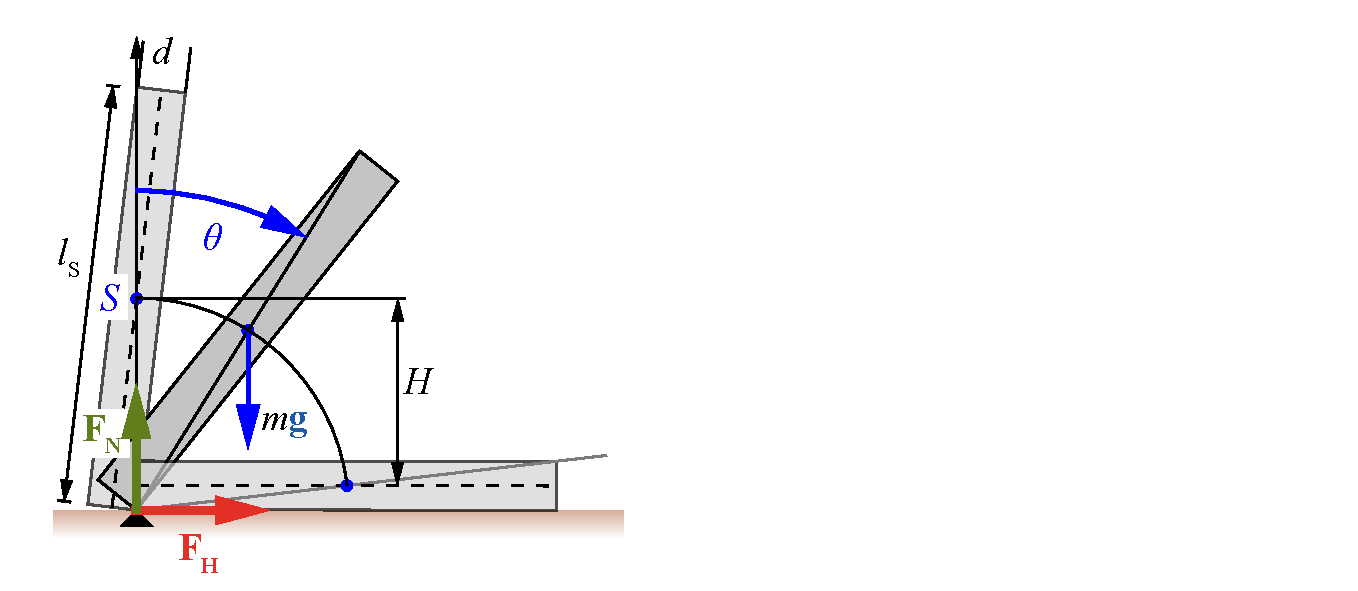
\includegraphics[width=\textwidth]{FallingRod08.pdf}
  \caption[Geometrie beim umfallenden Smartphone.]{Geometrie und physikalische Gr��en beim umfallenden Smartphone.} \label{abb:bew_fallingrod08}
\end{figure}

\newpage 

\subsection{Physikalische Kreisel-Spielzeuge und verwandte Themen} \label{kap:bew_apps_top}


\subsubsection{Rollende Zylinder, Garnrollen, Jo-Jos}

Der rollende Zylinder und das Jo-Jo sind in Lehrb�chern oft behandelte
Probleme. Generell sind physikalische Spielzeuge ungemein instruktiv und man
gewinnt auch ohne analytische Behandlung oft sehr tiefe Einblicke in und ein
intuitives Verst�ndnis f�r die grundlegenden Gesetze der Physik.
Wir empfehlen als Einstiegsliteratur besonders \cite{Ucke2011, Schlichting2016} und 
wollen hier einige der bekannten und weniger bekannten Effekte
etwas analytischer und auch quantitativer betrachten.

\subparagraph{\textbf{Garnrolle}}

    Wir beginnen zun�chst mit dem in vielen Lehrb�chern behandelten Beispiel
    der Garnrolle, das \ua f�r das Verst�ndnis des Jo-Jos hilfreich ist.
    Wie man an \figref{bew_Zylinder01} sieht, ist in beiden F�llen (a,b) das Drehmoment
    \[
    \vec{M}_\text{D}=\vec{r}\times\vec{F}
    \]
    so gerichtet, dass die Garnrolle nach rechts rollt. Im Fall c ist beim Grenzwinkel
    \[
    (90\,^\circ-\theta_\text{C}) = \arcsin\frac{R_i}{R_a}
    \]
    kein Rollen m�glich, da das Drehmoment in dieser Situation 0 ist,
    f�r $\theta>\!\theta_\text{C}$ wird die Garnrolle nach links rollen.

\begin{figure}
  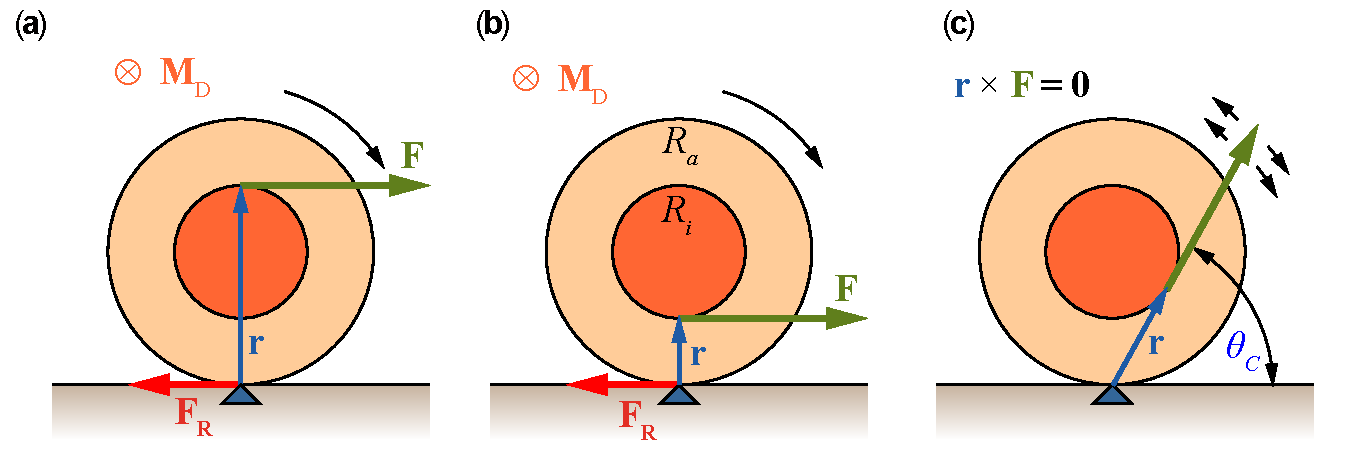
\includegraphics[width=\textwidth]{Garnrollen.pdf}
  \caption[Drehmomentwirkung an einer Garnrolle.]{Drehmomentwirkung an einer Garnrolle. H�ufig gestellte Quizfrage: Wohin rollt die Garnrolle? \fa \fb In beiden F�llen rollt die Garnrolle (sofern man nicht zu heftig daran zieht) nach rechts. \fc Ab einem kritischen Winkel $\theta_\text{C}$ wird die Garnrolle nach links rollen.} \label{abb:bew_Zylinder01}
\end{figure}

\subparagraph{\textbf{Jo-Jo}} \label{kap:bew_JoJo}
	
	Das Jo-Jo und das verwandte Diabolo (\figref{bew_Zylinder10}\,a,b) waren und sind zwei beliebte physikalische Spielzeuge, die dennoch relativ selten in der physikalischen Lehrliteratur behandelt werden.
        Die Zwangsbedingungen f�r die Bestimmung der Lagrange-Funktion des Jo-Jos (\figref{bew_Zylinder10}) haben wir bereits in \probref{bew_Zwangsbedingungen} hergeleitet. 

\begin{figure}
  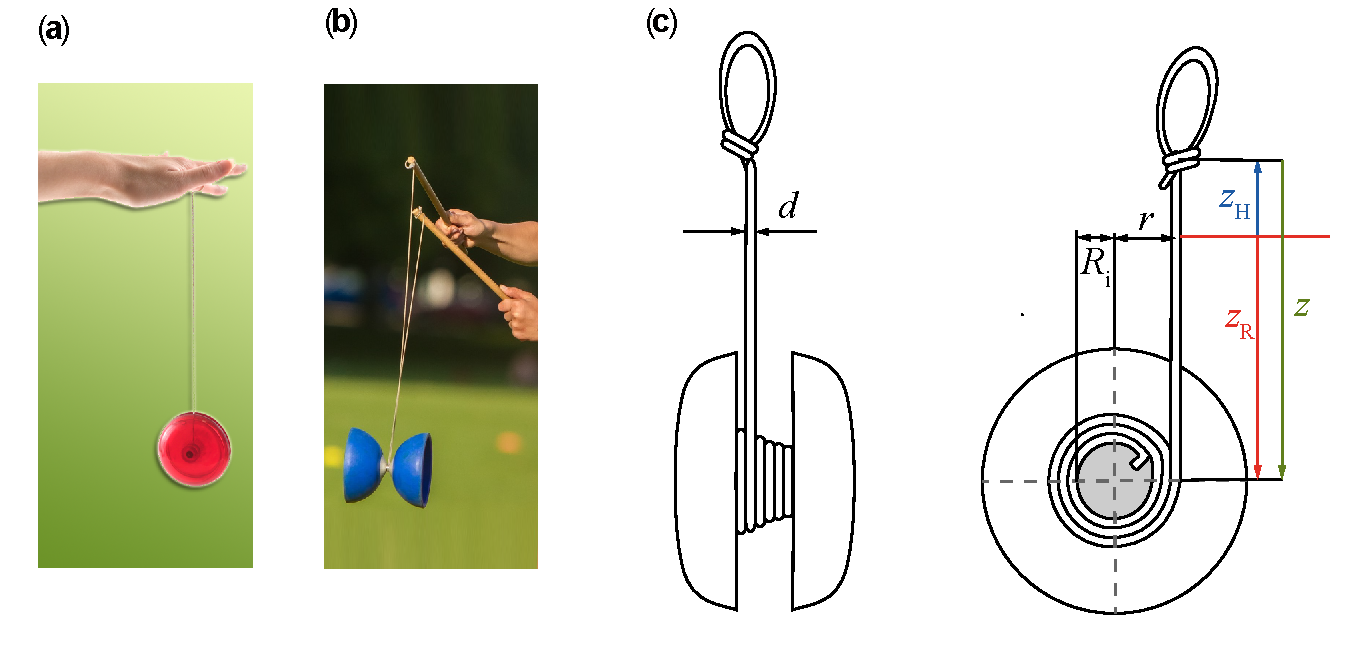
\includegraphics[width=\textwidth]{Zylinder10.pdf}
  \caption[Geometrische und physikalische Gr��en des Jo-Jos.]{Geometrische und physikalische Gr��en des Jo-Jos. \fa �bliche Ausf�hrungsform des Jo-Jos. \fb Verwandt mit dem Jo-Jo ist das Diabolo, dass aus einem Doppelkegel besteht, welcher auf ein Seil gesetzt wird, das an seinen Enden an zwei Handst�cken befestigt ist. Durch Bewegen des Seils wird das Diabolo in Rotation versetzt und damit als Kreisel im Raum stabilisiert.  \fc Im linken Teil des Bildes ist der Fadenkanal des Jo-Jos zu sehen, im rechten Teil des Bildes die Definition der im Folgenden verwendeten Gr��en: $R_\text{i}$ Wellenradius, $r=r(z)$ Spulenradius, $d=d_\text{eff}$ effektive Fadendicke, $z_\text{F}$ Fallh�he, $z_\text{H}$ Steuergr��e der Hand und $z$ Abwickell�nge des Jo-Jos (nach \cite{Buerger1983}).}
	\label{abb:bew_Zylinder10}
\end{figure}

	Dort haben wir aber die Fadendicke als Null angenommen.
    Diese wollen wir jetzt ber�cksichtigen und auch, dass mehrere Lagen des aufgewickelten
    Fadens �bereinander auf dem Wellenk�rper Platz finden (\figref{bew_Zylinder10}\,c). Daraus resultiert ein ver�nderlicher Spulenradius $r=r(z)$, ebenso wie eine effektive Fadenl�nge. Aus (\figref{bew_Zylinder10}\,c) sehen wir, dass sich bei einer regelm��igen Wicklung eine \anf{effektive Dicke} $d_\text{eff}$ des Fadens einf�hren l�sst, die durch
    \begin{align}
      \pi r^2 = \pi R_\text{i}{}^2 + d_{\text{eff}} \,(l_\text{S}-z) \label{eq:bew_JoJo01}
    \end{align}
    gegeben ist \cite{Buerger1983}. $l_\text{S}$ ist die Gesamtl�nge der Schnur und es gilt
    \[
    r_{\min} = r(z=l_\text{S}) = R_\text{i},\quad \text{\bzw} \quad r_{\max}=r(z=0) = \sqrt{R_\text{i}{}^2 + d_{\text{eff}} \,l_\text{S}/\pi }\,.
    \]
    Typische Werte sind $r_{\min}=\SI{0.3}{\centi\metre}$ und  $r_{\max}=\SI{1.3}{\centi\metre}$
    f�r $l_\text{S}=\SI{100}{\centi\metre}$, womit $d_{\text{eff}}=\SI{0.05}{\centi\metre}$ gilt.
    Die Lagrange-Gleichung 1.\ Art lautet dann
    \begin{align}
      m\ddot z&=mg-F_\text{T} ~~~\text{mit}~~~J\frac{\ddot z}{r^2(z)} = F_\text{T}\,,  \label{eq:bew_JoJoLGL}
    \end{align}
    wobei die Zwangsbedingung hier die Rollbedingung ist und die Zwangskraft $F_\text{T}$, die das Drehmoment auf die Jo-Jo-Scheibe verursacht.
    F�r das Jo-Jo nehmen wir zun�chst die Hand als ruhend an ($z_\text{H} = 0$).
    In diesem Fall ist $z_\text{F}=z$ und indem wir $\ddot z$ eliminieren, erhalten wir $F_\text{T}(z)$:
    \begin{align}
      F_\text{T}(z) = m g \frac{1}{1+m\,r(z)^2/J} = m g\frac{1}{1+2r(z)^2/R_a{}^2}\,~~\text{f�r}~~J\approx \frac 12\,m\, R_a{}^2\,. \label{eq:bew_JoJo08}
    \end{align}
    Dies gilt f�r $z\leq l_\text{S}$. 
    Da wir zun�chst Energieerhaltung annehmen, k�nnen wir schreiben:
    \begin{align}
      \frac m2v^2+\frac {J}{2}\omega^2-mg z = E\,.\label{eq:bew_JoJo02}
    \end{align}
    Hierin ist $v=\dot{z}$ die Schwerpunktsgeschwindigkeit,
    die beim einfachen Fallen, \dh ohne Steuerung durch die Hand,
    wegen $z=z_\text{F}$ nach der Fallstrecke $z$ erreicht wird.
    Aus der Rollbedingung $|v|=r|\omega |$ folgt dann
    \begin{align}
      v (z) =\pm\sqrt{2gz}\frac1{\sqrt{1+J/\lk mr^2(z)\rk}}\,,\label{eq:bew_JoJo03}
    \end{align}
    das Jo-Jo f�llt also durch das Wirken der Fadenspannung langsamer als ein frei fallender K�rper, was leicht einsichtig ist, da ja auch Energie in Rotation
    umgesetzt wird. Die Geschwindigkeit erreicht ein Maximum und f�llt dann wieder ab
    (\figref{bew_Zylinder11}).%
    \footnote{Streng genommen ist $J$ auch eine Funktion von $z$.
    Wenn wir die Masse des Fadens als sehr viel kleiner
    als die Masse der Jo-Jo Scheibe annehmen,
    k�nnen wir aber $J$ als konstant annehmen.}

\begin{figure}
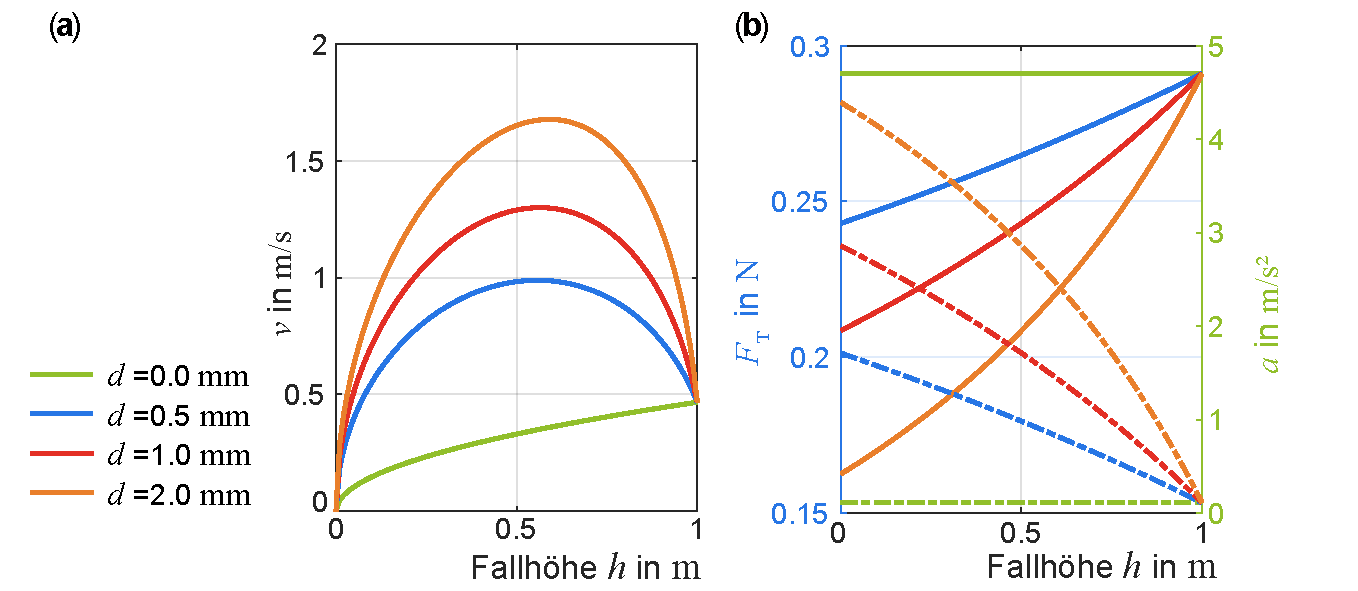
\includegraphics[width=\textwidth]{Zylinder11.pdf}
\caption[Geschwindigkeit, Fadenspannung und Beschleunigung des Jo-Jos.]{\fa Geschwindigkeit, sowie \fb Fadenspannung und Beschleunigung des Jo-Jos als Funktion der H�he. Als Parameter ist die Fadendicke $d$ angegeben. Die gr�ne Kurve beschreibt f�r eine effektive Fadendicke von Null das sogenannte akademische Jo-Jo.} \label{abb:bew_Zylinder11}
\end{figure}

    Wir schreiben Gl. \eqref{eq:bew_JoJo03} als
    \begin{align}
      \D t = \frac{\D z}{\sqrt{2gz}}\sqrt{1+ J/\lk mr^2(z) \rk}\,,
      \label{eq:bew_JoJo04}
    \end{align}
    substituieren
    \begin{align*}
      r^2(z) &= R_\text{i}{}^2+d(l_\text{S}-z)\,,~~ z = \frac{\pi r_{\max}{}^2}d\sin^2\psi\,,\\
			\phi &= \arccos\frac{r_{\min}}{r_{\max}}\,~~ \text{und}~~
			k=\frac{1}{\sqrt{1+J/\lk m\,r_{\max}{}^2 \rk}}\,,
    \end{align*}
    und erhalten nach Integration (Nachrechnung in \probref{bew_JoJoDynamik})
    \begin{align}
      t=\bigintsss_{\,0}^{t} \D t^\prime=\sqrt{\frac{2\pi}{g\,d}}\frac{r_{\max}}k
      \bigintsss_{\,0}^\phi \sqrt{1-k^2\sin^2\psi}\:\D \psi = E(\phi,k)\,.
      \label{eq:bew_JoJo05}
    \end{align}
    $E(\phi,k)$ ist das \textit{elliptisches Integral der 2. Art} \index{Integral!elliptisches} \cite{Gradshteyn1980, Olver1992}, das auch in \matlab{} hinterlegt ist.
    Alternativ l�sst sich nat�rlich auch \eqref{eq:bew_JoJoLGL} numerisch integrieren (\mscr{} \mlbewref{JoJo01.m})
    Damit haben wir die Phase des Abspulens beschrieben,
    da die Umkehrung von $t=t(\psi(z))$ uns $z(t)$ liefert.

    Ist das Jo-Jo abgespult $(t=t_u,\, z=l_\text{S})$, dann wendet das Jo-Jo
    (\figref{bew_Zylinder13}) und die Bewegung des Jo-Jos wird jetzt
    durch eine Drehung �ber
    \[
    z=l_\text{S}+R_\text{i}\cos\varphi  ~~~\text{mit}~~~ -\pi/2 \leq \varphi \leq \pi/2
    \]
    beschrieben. In dieser Phase kann man das Jo-Jo als physikalisches Pendel betrachten
    \cite{Minkin2021}.
 %
\begin{figure}
\begin{minipage}{\textwidth}
\leftfigure{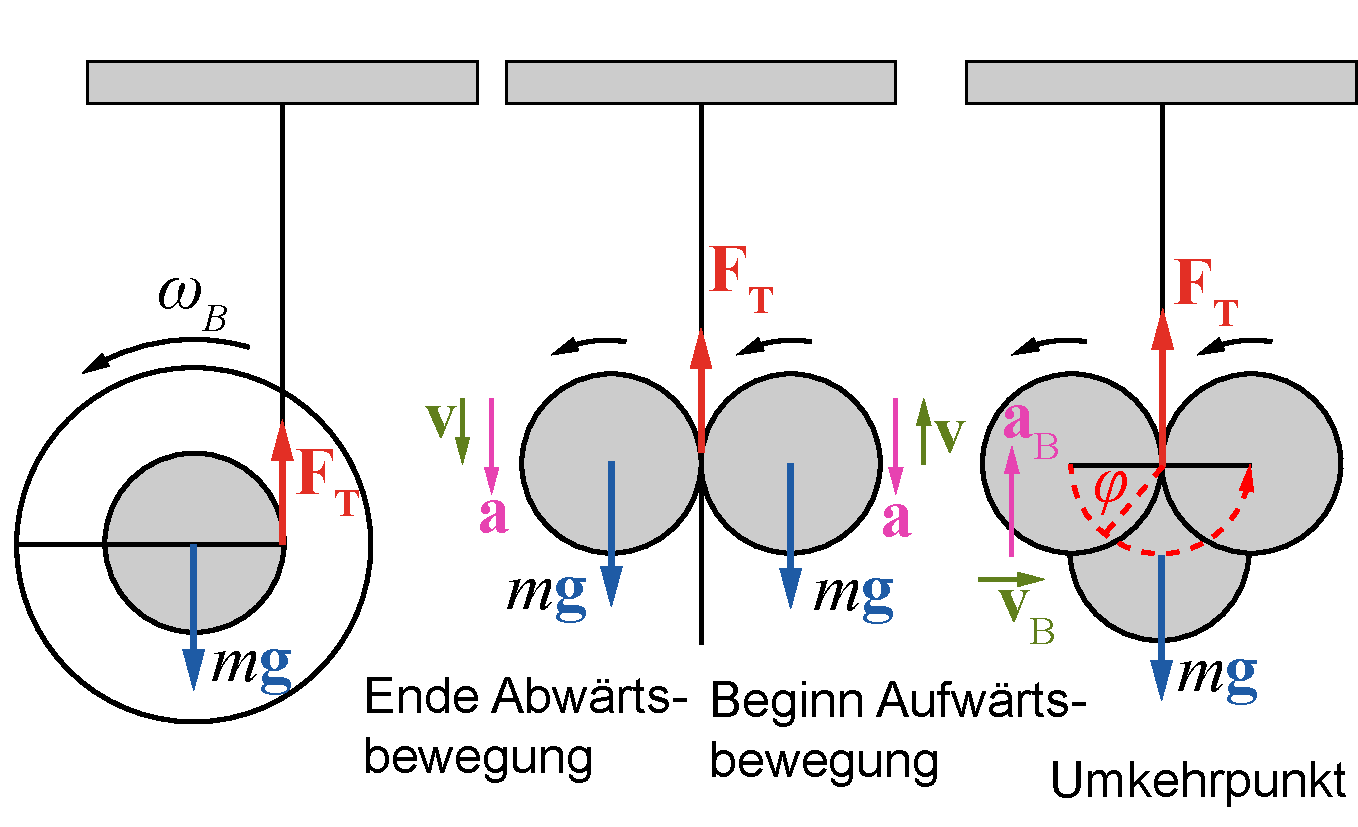
\includegraphics[width=0.5\textwidth]{Zylinder13.pdf}}%
\hspace{\fill}
\rightfigure{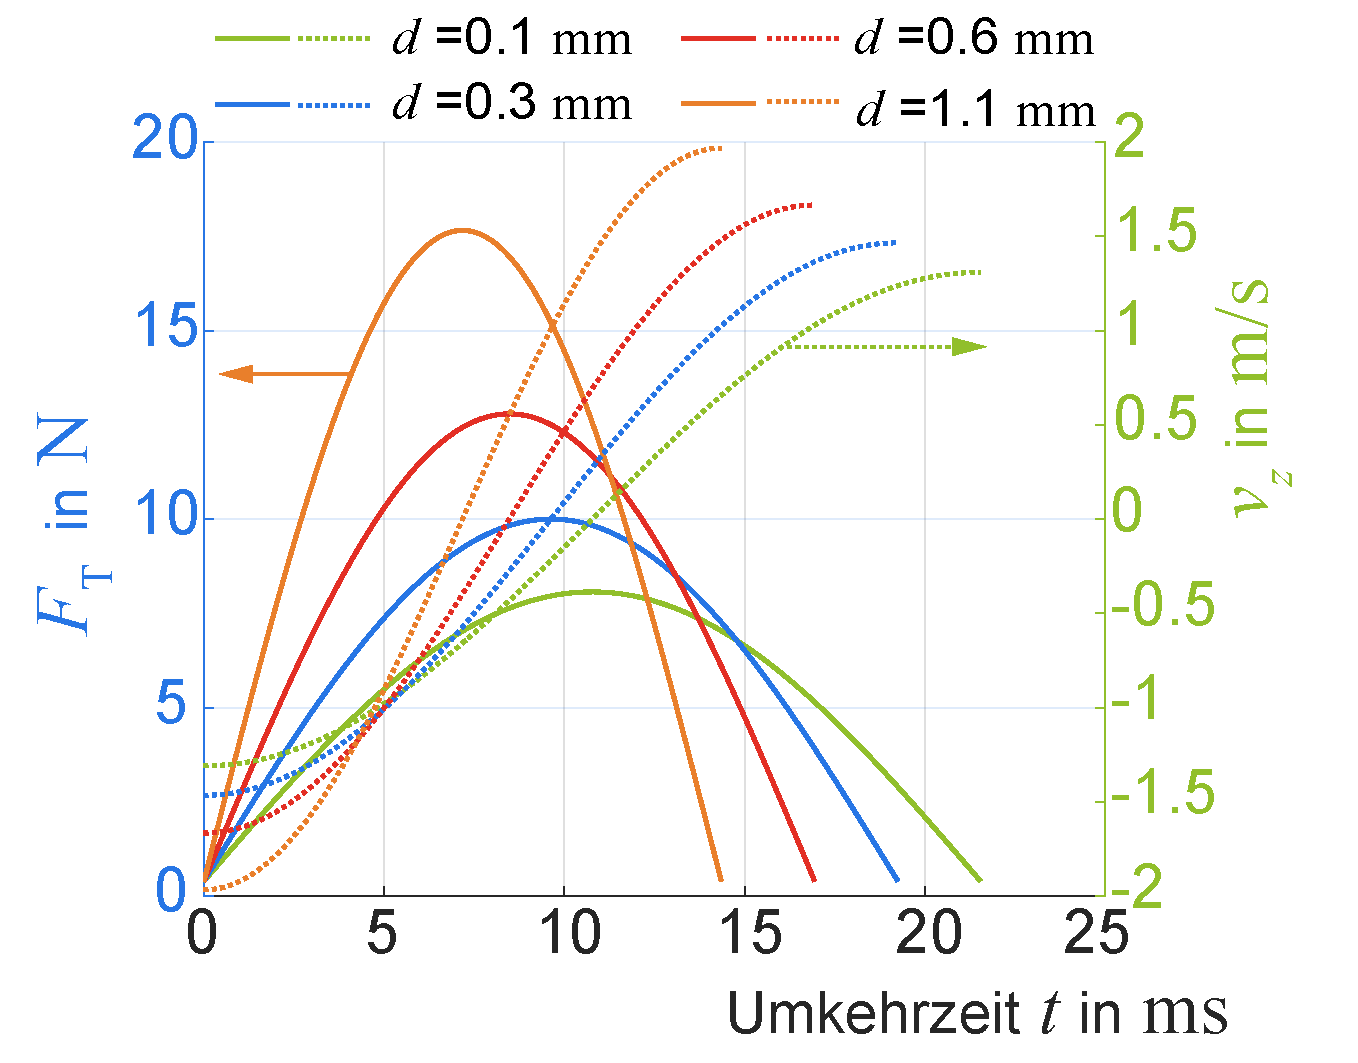
\includegraphics[width=0.5\textwidth]{Zylinder14.pdf}}
\leftcaption[Verhalten des Jo-Jos am Wendepunkt.]{Verhalten des Jo-Jos am Wendepunkt. Das Jo-Jo verh�lt sich wie ein physikalisches Pendel. $\vec{F}_\text{T}$ ist die Zugspannung im Faden, $\vec a$ die Beschleunigung, $\vec v$ die Geschwindigkeit des Massenmittelpunktes. Am Umkehrpunkt addiert sich die Zentripetalbeschleunigung zu $\vec g$ hinzu.} \label{abb:bew_Zylinder13}
\rightcaption[Fadenspannung und Geschwindigkeit des Jo-Jos am Wendepunkt.]{Fadenspannung und Geschwindigkeit des Jo-Jos am Wendepunkt.} \label{abb:bew_Zylinder14}
\end{minipage}
\end{figure}

    Wie in \figref{bew_Zylinder13} gezeigt, rotiert der Jo-Jo-K�rper um den mehr oder weniger
    gestreckten Faden.\footnote{Das ist umso mehr erf�llt, je l�nger der Faden ist, also wenn
    $l_\text{S}\gg R_\text{i}$.} Die halbe Schwingungsfrequenz $\omega_B$ kann man aus der Energieerhaltung f�r das physikalische Pendel gewinnen:
	\[ \omega_B = \sqrt{\frac{2mg l_\text{S}}{J}} \sqrt{\frac{1+\frac{R_\text{i}}{2} \cos\varphi}{1+\frac{mR_\text{i}{}^2}{J} \sin\varphi}} \approx \sqrt{\frac{2mg l_\text{S}}{J}} \; .
	\]
        Man kann also die Kreisfrequenz also n�herungsweise als konstant ansehen. Damit ergeben sich \anf{Wendezeiten} $T_P=\pi/\omega_B$ von wenigen $\SI{}{\milli\s}$ und f�r die Tangentialgeschwindigkeit $v_B$ \bzw die Zusatzbeschleunigung $a_B$ am unteren Umkehrpunkt damit
   \begin{align}
     v_B \approx \omega_B\,R_\text{i} ~~\text{\bzw} ~~ a_B \approx \omega_B{}^2\,R_\text{i}\,. \label{eq:bew_JoJo07}
   \end{align}
	  Der Jo-Jo-Spieler wird dieses Umkehren durch einen kr�ftigen Zug am Faden, also in der Fadenspannung merken. 
    In der Umkehrphase f�r $z>l_\text{S}$ m�ssen wir also die $z$-Komponente der radialen Zentripetalkraft zur Fadenspannung \eqref{eq:bew_JoJo08} addieren.
    Wir berechnen $z(t)$ f�r $z\leq l_\text{S}$ aus der Lagrange-Gleichung \eqref{eq:bew_JoJoLGL} und f�r $z>l_\text{S}$ aus der L�sung f�r
    das physikalische Pendel \eqref{eq:bew_PhysPendel02} mit der Anfangsgeschwindigkeit $v_u$ und der Auslenkung $-\pi/2$.
    Das Ergebnis ist in \figref{bew_Zylinder14} dargestellt. Man erkennt, dass die Wendezeit
    nur einige Hundertstelsekunden betr�gt, die zus�tzliche Spannung im Faden wird entsprechend gro�.\\ 
		
    Zum Schluss wollen wir noch kurz das \anf{angeregte} Jo-Jo betrachten.
    Bei dieser Spielart ersetzt der Jo-Jo-Spieler den unvermeidbaren Reibungsenergieverlust beim Auf-und-Ab
    durch eine geschickt gesteuerte Bewegung des Fadenendes mit seiner Hand.
    F�r das getriebene Jo-Jo ist die Fallh�he $z_\text{R}$ im Raumkoordinatensystem dann verschieden von der Abwickell�nge $z$.
    Es gilt  $z=z_\text{R}+z_\text{H}$
    (\figref{bew_Zylinder11}), wo $z_\text{H}$ die Bewegung des Aufh�ngepunktes durch die steuernde Hand ist. Die Bewegungsgleichung gewinnt man unter Beachtung der Rollbedingung
    $|\dot z|=r|\dot\varphi|=\sqrt{R_\text{i}{}^2+(l_\text{S}-z)\, d/\pi}$
    aus der Lagrange-Funktion:
    \begin{align}
      \mathcal{L}_\text{S}(z,\dot z) = \frac m2\,(\dot z-\dot z_\text{H})^2
      + \frac J2\left(\frac{\dot z}r\right)^2 + m\,g\,(z-z_\text{H})\,,
      \label{eq:bew_JoJo09}
    \end{align}
    woraus wir die Lagrange-Gleichung
    \begin{align}
      \frac{\D}{\D t}\left[\left(1+\frac J{m\,r(z)^2}\right)\dot z^2\right]
      = 2\,(g+\ddot z_\text{H})\,\dot z \label{eq:bew_JoJo10}
    \end{align}
    gewinnen. Das l�sst sich integrieren: 
    \begin{align}
      \dot z^2 = \frac{2\left[g\,z+\bigintsss_{\,0}^t\ddot z_\text{H}(t')\,\dot{z}(t')\,\D t'+C\right]}{1+J/\lk mr^2(z) \rk}\,.
      \label{eq:bew_JoJo11}
    \end{align}
    $C$ ist eine Integrationskonstante, die sich aus den Anfangsbedingungen ergibt.
    Die Anregungsgr��e $z_\text{H}(t)$ bestimmt also die Bewegung des Jo-Jos, genauer das Integral
    \[
    \bigintsss_{\,0}^t\ddot z_\text{H}(t')\,\dot{z}(t')\,\D t' = \bigintsss_{\,0}^z\ddot z_\text{H}(z^\prime)\,\D z^\prime\,,
    \]
    welches die Energiezufuhr pro Masseneinheit auf dem durchlaufenen Weg der Jo-Jo-Schnur bedeutet.
    Energiezufuhr hei�t $\ddot z_\text{H}>0$, \dh eine Beschleunigung der Hand nach oben, wenn $z$ w�chst
    (Abwicklungsphase) und $\ddot z_\text{H}<0$ f�r $\dot z<0$ (Aufwicklungsphase).
    In \probref{bew_JoJoDynamik} wird die Dynamik des Jo-Jos $z(t)$ als Funktion der 
    Anregungsfunktionen $z_\text{H}(t)$ berechnet. Man erkennt, wie wichtig die Synchronisation der Hand mit der 
    Auf-und-Abbewegung des Jo-Jos ist (siehe auch \mscr{} \mlbewref{JoJo02.m}).


\subsubsection{Rollende Zylinder, Scheiben und Reifen} \label{kap:bew_rolling_disc}

\subparagraph{\textbf{Rollende Zylinder auf der schiefen Ebene}}	

Die Bewegung rollender Objekte auf der schiefen Ebene schafft es trotz ihrer
Einfachheit immer wieder zu faszinieren und manchmal mit der Intuition auf falsche Schl�sse zu kommen.
Typischerweise betrachtet man mehrere Objekte derselben
Masse und desselben Radius, aber unterschiedlicher Masseverteilung. L�sst man
sie die Ebene hinunterrollen, stellt sich die Frage, welches Objekt am
ehesten unten ankommt. Das wollen wir f�r die Hohlkugel, die Vollkugel,
einen Hohlzylinder, einen Vollzylinder und einen mit Fl�ssigkeit gef�llten
Zylinder betrachten. Dazu f�hren wir auf der schiefen Ebene
(\figref{bew_Zylinder05}) eine Koordinate $s$ entlang der Ebene ein, die an der
oberen Kante beginnt. $s$ stehe senkrecht auf dieser Kante.

\begin{figure}
  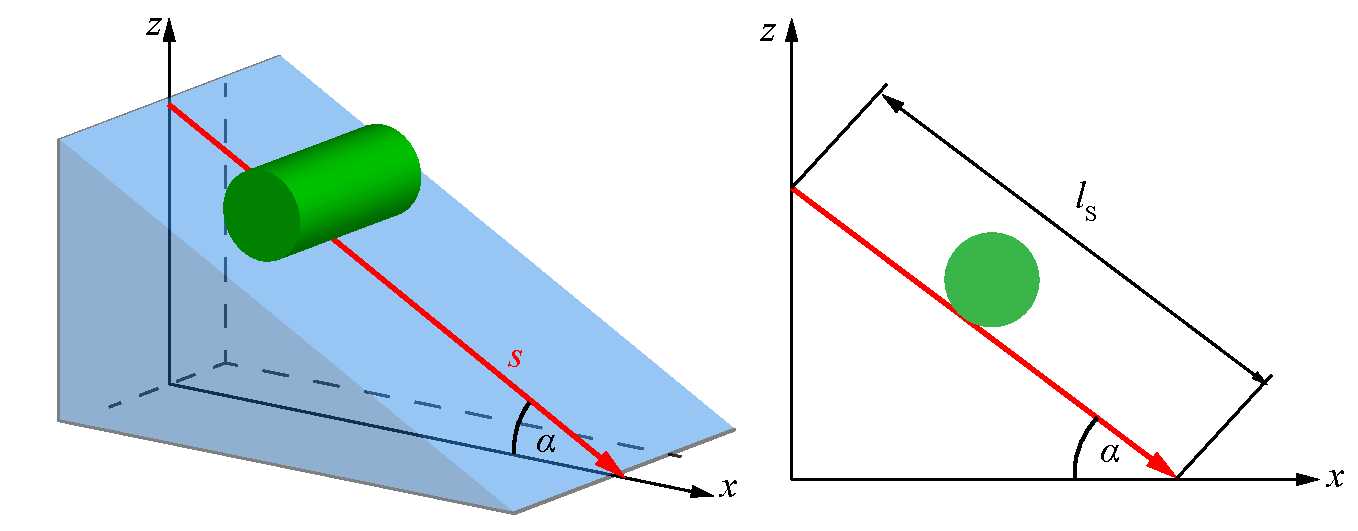
\includegraphics[width=\textwidth]{RollZylGeometrie.pdf}
  \caption[Geometrie des rollenden Zylinders.]{Geometrie des rollenden Zylinders.} \label{abb:bew_Zylinder05}
\end{figure}

Die Koordinate $s$ ist gut zur Beschreibung des Problems geeignet, denn zum
Aufstellen der Lagrange-Funktion ben�tigen wir die Translations- und
Rotationsenergien,
\begin{equation*}
  T = \frac{1}{2} m \dot{s}^2 + \frac{1}{2} J \omega^2 \; .
\end{equation*}
Wir wollen zun�chst davon ausgehen, dass die Reibung so stark ist, dass keines
der Objekte zu rutschen beginnt. Dann gilt die Rollbedingung $s = R \varphi$
mit dem identischen Radius $R$ aller Objekte. Aus dieser folgt $\omega =
\dot{\varphi} = \dot{s}/R$ und somit f�r die kinetische Energie
\begin{equation*}
  T = \frac{1}{2} m \dot{s}^2 + \frac{1}{2} \frac{J}{R^2} \dot{s}^2
  = \frac{1}{2} \left ( m + \frac{J}{R^2} \right ) \dot{s}^2 \; .
\end{equation*}
Das Potential ergibt sich zu
\begin{equation*}
  U = mg z  = mg (l_\text{S}-s) \sin\alpha
\end{equation*}
mit der Gesamtl�nge $l_\text{S}$ der Ebene. Es folgen die Lagrange-Funktion
\begin{equation*}
  \mathcal{L} = \frac{1}{2} \left ( m + \frac{J}{R^2} \right ) \dot{s}^2
  - mg (l_\text{S}-s) \sin\alpha
\end{equation*}
und die Bewegungsgleichung
\begin{equation*}
  \ddot{s} = \frac{mg}{m+J/R^2} \sin{\alpha} \;. 
\end{equation*}
Lassen wir alle Objekte an der oberen Kante ohne Anfangsgeschwindigkeit
starten, gilt $s(0) = \dot{s}(0) = 0$ und die L�sung der Bewegungsgleichung
lautet
\begin{equation*}
  s(t) = \frac{1}{2} \frac{mg}{m+J/R^2} \, t^2 \,\sin{\alpha}\;,
\end{equation*}
\bzw wir extrahieren daraus sofort die Zeit $t_L$, die das Objekt
ben�tigt, um die Strecke $l_\text{S}$ zur�ckzulegen und unten anzukommen,
\begin{equation*}
  t_L = \sqrt{ \frac{2 l_\text{S} \left ( m+J/R^2\right )}{mg
      \sin\alpha}} \;.
\end{equation*}

Es ist zu erwarten, dass das Objekt mit dem geringsten Tr�gheitsmoment die
k�rzeste Zeit ben�tigt. Hier geht am wenigsten Energie in die Rotation und
die meiste Energie steht f�r die Translationsbewegung zur Verf�gung. Folglich
kommt das Objekt am ehesten unten an. Aus den Tr�gheitsmomenten folgt dann als 
Reihenfolge (vergleiche �bung
\ref{prob:bew_traegheitsmomente}) f�r die Ankunft am unteren Ende:

\begin{enumerate}
\item Vollkugel, $J = \frac{2}{5} m R^2$
\item Vollzylinder, $J = \frac{1}{2} m R^2$
\item Hohlkugel mit Schalendicke $d \ll R$, $J = \frac{2}{3} m R^2$
\item Hohlzylinder mit Manteldicke $d \ll R$, $J = m R^2$
\end{enumerate}

Au�en vor gelassen haben wir bisher den mit einer Fl�ssigkeit gef�llten
Hohlzylinder. Dieser ist in unserer bisherigen Betrachtung noch nicht
enthalten, denn wir sind von einem starren K�rper ausgegangen, dessen gesamte
Masse immer der Drehbewegung folgt. Das ist hier jedoch nicht erf�llt. Die
Fl�ssigkeit beginnt zwar durch die Reibungskr�fte am Rand, sich ebenfalls
zu bewegen, tut das jedoch nur langsam. Da die Drehbewegung des Rands immer
schneller wird, wird die Fl�ssigkeit sich zu jedem Zeitpunkt langsamer drehen als die
H�lle. Es geht hier also deutlich weniger Energie in die Rotation als beim
entsprechend schweren Vollzylinder. Die Einsortierung in die oben genannte
Reihenfolge h�ngt nat�rlich davon ab, wie gro�
die Z�higkeit\index{Viskosit�t}\index{Z�higkeit} der Fl�ssigkeit
und der Massenanteil der H�lle
ist, denn diese stellt eine Art Hohlzylinder dar. Typischerweise liegt jedoch
der gr��te Teil der Masse -- man denke \zb an eine Konservendose -- in der
Fl�ssigkeit. In diesem Fall kann der fl�ssigkeitsgef�llte Zylinder durchaus
das schnellste Objekt sein. 

\subparagraph{\textbf{Rollende Scheiben und Reifen auf einer Ebene}}	

Wir wollen nun einen Schritt weiter gehen und rollende R�der \bzw Reifen
betrachten. Dies ist ein oft behandeltes
Beispiel. Wir wollen hier die wesentlichen Punkte, die f�r das Verst�ndnis wichtig
sind, nachvollziehen und verweisen f�r einige wenige ausgelassene Rechenschritte den interessierten
Leser auf die Literatur. Ausf�hrliche Darstellungen finden sich \zb in \cite{Kuypers2012, Morin2008}.
Der Einfachheit halber modellieren wir diese durch eine
Kreisscheibe. Das Problem ist im Wesentlichen dasselbe, nur die
Tr�gheitsmomente unterscheiden sich, weil bei einem Rad der gr��te Teil der
Masse am �u�eren Radius konzentriert ist. \\
Im Gegensatz zu Zylindern tritt bei R�dern oder Kreisscheiben ein weiterer
Freiheitsgrad auf. Zylinder liegen immer stabil mit einer Achse parallel zur
Figurenachse auf dem Boden auf. Bei einer Kreisscheibe ist das nicht so, diese
kann umkippen und ihre Lage im Raum muss gesondert betrachtet werden, wie in \figref{bew_LageKreisscheibe} dargestellt.

\begin{figure}
  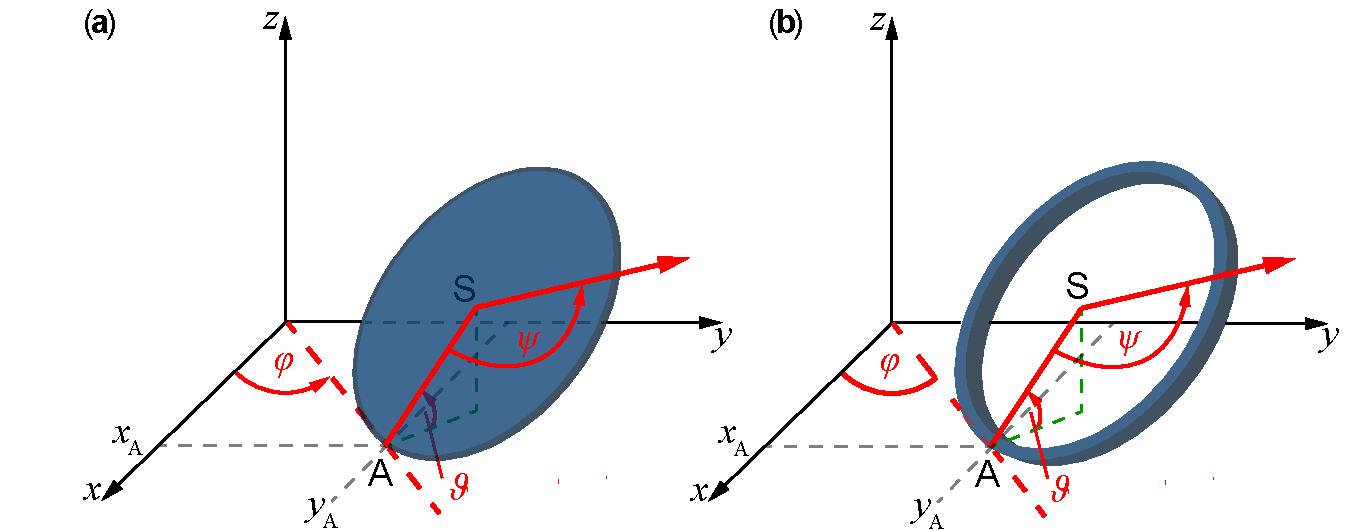
\includegraphics[width=\textwidth]{KreisscheibeLage.pdf}
  \caption[Rollende Kreisscheiben und Ringe.]{Rollende Kreisscheiben und Ringe.
    Da Kreisscheiben und Ringe ideale symmetrische Kreisel darstellen, die
    sich prinzipiell um alle drei Achsen frei drehen k�nnen, sind die Eulerwinkel
    $\varphi$, $\vartheta$, $\psi$ ideal zur Beschreibung ihrer jeweiligen Lage geeignet.}
  \label{abb:bew_LageKreisscheibe}
\end{figure}

Wir verwenden f�r die Beschreibung der Lage der Kreisscheibe die drei
Eulerwinkel $\varphi$, $\vartheta$, $\psi$ aus
\kapitel{bew_EulerWinkel}. Sie sind ideal geeignet, da die Kreisscheibe einen
symmetrischen Kreisel darstellt, der sich prinzipiell um alle drei Achsen
frei bewegen kann. Die einzige Einschr�nkung besteht darin, dass wir sie
immer auf dem Boden, \dh in der $x$-$y$-Ebene rollen lassen wollen. 
Dadurch ergibt sich eine Zwangsbedingung, die die Koordinaten
$x_\mathrm{A}$ und $y_\mathrm{A}$ des Auflagepunktes mit den Eulerwinkeln
verkn�pft. Diese Relation kann jedoch nur differentiell angegeben werden,
da sich alle Variablen mit der Zeit �ndern,
\begin{subequations}
  \begin{align}
    \D x_\mathrm{A} &= - R \cos\varphi\, \D \psi \qquad \text{bzw.} \qquad
                      \dot{x}_\mathrm{A} + R \cos\varphi\, \dot{\psi} = 0 \; ,
                      \label{eq:bew_ZBrollendeScheibe1} \\
    \D y_\mathrm{A} &= - R \sin\varphi\, \D \psi \qquad \text{bzw.} \qquad
                      \dot{y}_\mathrm{A} + R \sin\varphi\, \dot{\psi} = 0 \; .
                      \label{eq:bew_ZBrollendeScheibe2}
  \end{align}
\end{subequations}
Dies ist ein typisches Beispiel f�r eine nicht-holonome Zwangsbedingung.

Die Rotationsenergie l�sst sich mit den Tr�gheitsmomenten $J_1 = J_2 = J_{12}$
und $J_3$ im k�rperfesten System mit $T_\mathrm{rot} = \frac{1}{2} J_{12}
( \omega_1'^2 + \omega_2'^2 ) + \frac{1}{2} J_3 \omega_3'^2$ angeben. Mit
\eqref{eq:bew_EulerWinkel} ergibt sich daraus
\begin{align}
  T_\mathrm{rot} &= \frac{1}{2} J_{12} \left ( \dot{\vartheta}^2 + \sin^2
  \vartheta \, \dot{\varphi}^2 \right ) +  \frac{1}{2} J_{3} \left (
  \cos^2 \vartheta \, \dot{\varphi}^2 + 2 \cos\vartheta\, \dot{\varphi} \dot{\psi}
                   + \dot{\psi}^2 \right ) \notag \\
  \intertext{\bzw mit $J_{12} = mR^2/4$ und $J_3 = mR^2/2$ f�r eine Kreisscheibe}
  T_\mathrm{rot} &= \frac{mR^2}{8} \left ( \dot{\vartheta}^2 + ( 1 + \cos^2
                   \vartheta ) \dot{\varphi}^2 +
                   4 \cos\vartheta\, \dot{\varphi} \dot{\psi}
                   + 2\, \dot{\psi}^2 \right ) \; .
                   \label{eq:bew_rollendeScheibe_rotE}
\end{align}

Hinzu kommt die Translationsenergie, die sich mit der Schwerpunktkoordinate
\begin{align*}
  x_\mathrm{S} &=  x_\mathrm{A} - R \cos\vartheta\,\sin\varphi \;, \quad
  y_\mathrm{S} =  y_\mathrm{A} + R \cos\vartheta\,\cos\varphi \;, \quad
  z_\mathrm{S} =  R \sin\vartheta
\end{align*}
zu
\begin{align}
\begin{split}
  T_\mathrm{trans} &= \frac{m}{2} \bigg ( \dot{x}_\mathrm{A}^2 +
    \dot{y}_\mathrm{A}^2 + R^2(\dot{\vartheta}^2 + \cos^2 \vartheta\,
    \dot{\varphi}^2 ) \\
		& \quad\quad\quad - 2 R \dot{x}_\mathrm{A} ( \cos\varphi\, \cos\vartheta\,
    \dot{\varphi} - \sin\varphi\, \sin\vartheta\, \dot{\vartheta} ) \\
    & \quad\quad\quad - 2 R \dot{y}_\mathrm{A} ( \sin\varphi\, \cos\vartheta\,
    \dot{\varphi} + \cos\varphi\, \sin\vartheta\, \dot{\vartheta} ) \bigg )
  \end{split}\label{eq:bew_rollendeScheibe_transE}
  \end{align}
ergibt, und das Potential
\begin{equation}
  U = m g z_\mathrm{S} =  m g R \sin\vartheta \; .
  \label{eq:bew_rollendeScheibe_Pot}
\end{equation}

Diese Gleichungen enthalten mit $x_\mathrm{A}$, $y_\mathrm{A}$, $\varphi$,
$\vartheta$ und $\psi$ f�nf Koordinaten, die jedoch nicht voneinander
unabh�ngig sind, sondern durch die differentiellen Zwangsbedingungen
\eqref{eq:bew_ZBrollendeScheibe1} und \eqref{eq:bew_ZBrollendeScheibe2}
miteinander verkn�pft sind. Die L�sung erfolgt deshalb �ber die Methode der Lagrange-Multiplikatoren 
�ber die Lagrange-Gleichungen erster Art (siehe \eqref{eq:bew_Lagrange_I} in \kap{bew_Lagrange_I}). Daraus lassen
sich f�r die drei Eulerwinkel die Differentialgleichungen
\begin{subequations}
  \begin{align}
    \sin\vartheta\, \ddot{\varphi} - 2 \dot{\psi}\dot{\vartheta} &= 0 \; , \\
    \ddot{\vartheta} +  \sin\vartheta\, \cos\vartheta\,
    \dot{\varphi}^2 + \frac{6}{5} \sin\vartheta\, \dot{\varphi}\,\dot{\psi}
    + \frac{4}{5} \frac{g}{R} \cos\vartheta &= 0 \; , \\
    \sin\vartheta\, \ddot{\psi} + \frac{5}{3}\, \sin^2\vartheta \ \dot{\varphi}\,
    \dot{\vartheta} + 2  \cos\vartheta\, \dot{\psi}\,\dot{\vartheta} &= 0 \;
                                                                       \label{eq:bew_ZBrollendeScheibe3}
  \end{align}
  \label{eq:bew_rollendescheibe_dgls}
\end{subequations}

ableiten, was wir in \probref{bew_scheibe} verifizieren wollen.
Die Position des Auflagepunktes $x_\mathrm{A}$,
$y_\mathrm{S}$ erh�lt man, indem man die Zwangsbedingungen
\eqref{eq:bew_ZBrollendeScheibe1} und \eqref{eq:bew_ZBrollendeScheibe2}
aufintegriert. 

\begin{figure}
  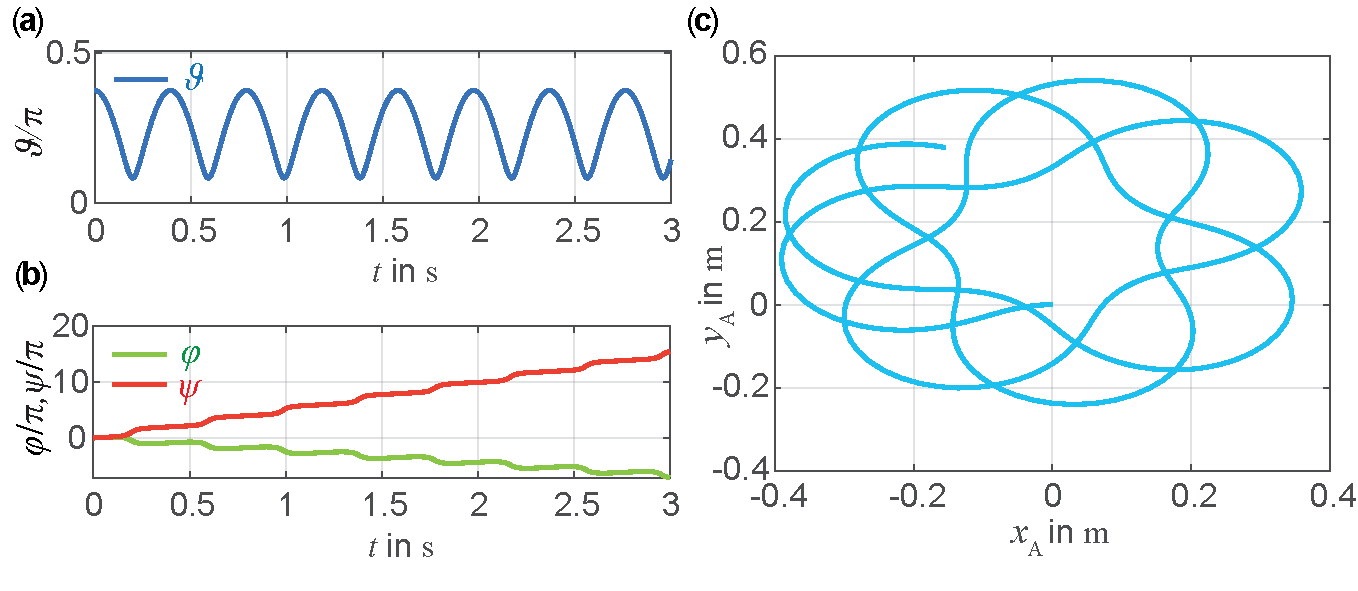
\includegraphics[width=\textwidth]{RollendeKreisscheibe.pdf}
  \caption[Bewegung einer rollenden Kreisscheibe.]{Bewegung einer rollenden
    Kreisscheibe mit $R=\SI{15}{\centi\metre}$ und den Anfangsbedingungen
    $\varphi = \psi = 0$, $\vartheta = 3\pi/8$, $\dot{\varphi} = \dot{\psi}
    = \SI{6}{\per\second}$, $\dot{\vartheta} = 0$ sowie $x_\mathrm{A}(0)
    =y_\mathrm{A}(0)=0$. \fa \fb Eulerwinkel und \fc Spur des Auflagepunktes in der $x$-$y$-Ebene. Die Scheibe beginnt zun�chst zu kippen. Dadurch
    steigt jedoch die Rollgeschwindigkeit und der Drehimpuls verhindert
    ein vollst�ndiges Umkippen. Die Schreibe richtet sich wieder auf. Dabei
    bewegt sie sich im Raum schlingernd fort.}
  \label{abb:bew_BewegungKreisscheibe}
\end{figure}

Diese Gleichungen wollen wir nun numerisch l�sen (siehe 
\mscr{} \mlbewref{RollendesRad.m}). F�r eine Kreisscheibe mit
dem Radius $R=\SI{15}{\centi\metre}$, die im
Ursprung startet ($x_\mathrm{A}(0)=y_\mathrm{A}(0)=0$), zu Beginn die
Neigung $\vartheta = 3\pi/8$ mit $\varphi = \psi = 0$ hat und sich mit den
Winkelgeschwindigkeiten $\dot{\varphi} = \dot{\psi} = \SI{6}{\per\second}$,
$\dot{\vartheta} = 0$ bewegt, ergibt sich der Fall, der in Abbildung
\figref{bew_BewegungKreisscheibe} dargestellt ist. Man erkennt deutlich in \figref{bew_BewegungKreisscheibe}a, wie die Kreisscheibe zun�chst beginnt zu kippen. Der
Winkel $\vartheta$ wird kleiner, was einer Ann�herung an die flach auf dem
Boden liegende Kreisscheibe entspricht. Dadurch wird die Rollbewegung jedoch
beschleunigt, die Ableitung der Winkel $\varphi$ und $\psi$ wird gr��er (\figref{bew_BewegungKreisscheibe}b).
Hier setzt sich nun der Drehimpuls durch. F�r ein weiteres Kippen m�sste (die
Scheibe rollt die ganze Zeit!) mehr kinetische Energie aufgebracht werden, als
durch das Gravitationspotential zur Verf�gung steht. Folglich kehrt die
Kippbewegung um und die Kreisscheibe richtet sich wieder auf. Das Spiel wiederholt sich mehrfach. Im Englischen wird das Ph�nomen \textit{wobbling disk} genannt.
Der Auflagepunkt legt dabei die Bewegung zur�ck, die in \figref{bew_BewegungKreisscheibe}c gezeigt ist. Man erkennt deutlich, wie die
Kreisscheibe sich in einer Schlingerbewegung vom Ursprung entfernt und sich
zeitweise wieder ann�hert. Sie umrundet dabei mehrfach ein sich langsam �nderndes Zentrum der Bewegung. 

Wir halten dabei fest, dass ein Rad zwar kippen kann, durch die Drehbewegung
und den dabei im System befindlichen Drehimpuls kann dieser Kippbewegung
jedoch eine Grenze gesetzt werden. Das Rad kann sich einigerma�en stabil
bewegen. Dies gilt umso mehr, je schneller es sich dreht. Wir werden darauf im Band III 
bei der Physik des Sports mehrfach zur�ck kommen.

\subsubsection{Der aufw�rts rollende Doppelkegel} \label{kap:bew_doublecone}

\subparagraph{\textbf{Grundlegende geometrische und energetische Betrachtungen}}

Bereits im 18.~Jahrhundert wurde dieses Experiment beschrieben,
das auch heute noch oft in den Experimentalphysikvorlesungen gezeigt wird.
Bei diesem rollt ein Doppelkegel scheinbar eine schiefe Ebene von allein hinauf
und scheint dabei dem Energiesatz zu widersprechen.
Die schiefe Ebene wird dabei von zwei Schienen gebildet,
die unter einem Winkel von $2\phi$ stehen (\figref{bew_doublecone01}). \\
Die physikalische Erkl�rung des Ph�nomens ist recht einfach
und \ua in \cite{Ucke1997, Ucke2011, Gallitto2011} beschrieben.
Sie besteht darin, dass beim Abrollen des Doppelkegels auf den Schienen
sein Schwerpunkt sich nach unten bewegt, da sich der Auflagepunkt (Rollpunkt) des Doppelkegels
mit dem Abrollen nach au�en zu den Kegelspitzen hin verschiebt. 

\begin{figure}
  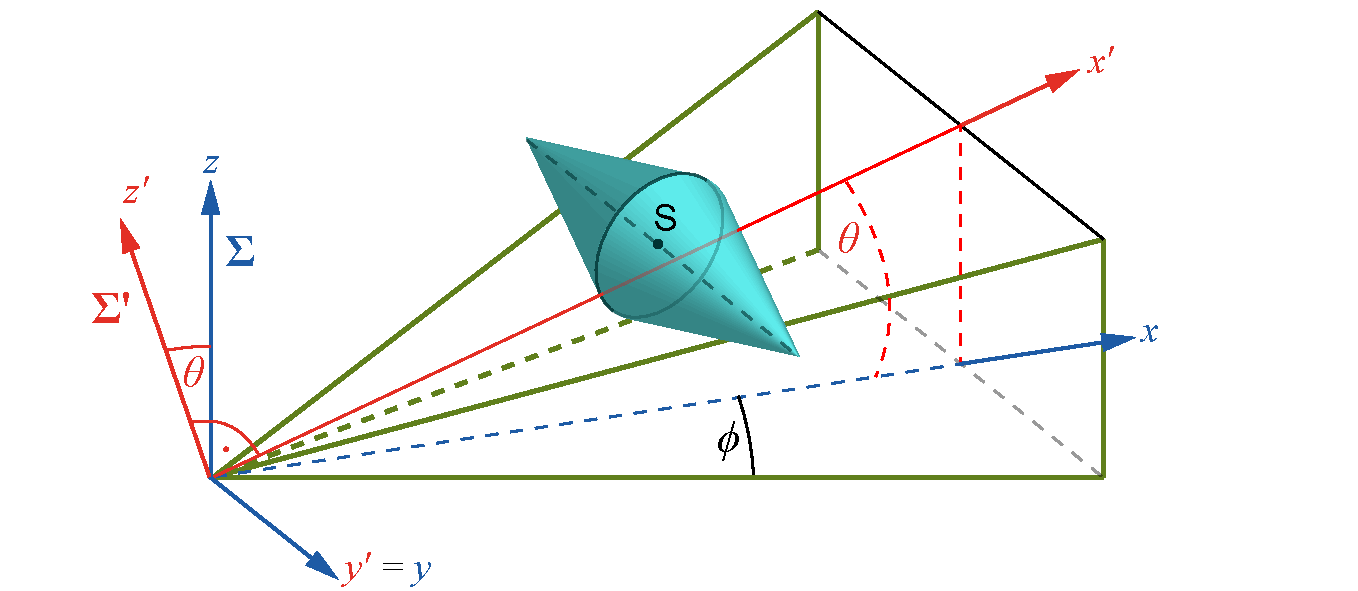
\includegraphics[width=\textwidth]{Doppelkegel01.pdf}
  \caption[Aufbau des aufw�rts laufenden Doppelkegels.]{Aufbau des aufw�rtslaufenden Doppelkegels auf einem Paar von Schienen, die unter einem �ffnungswinkel von $2\phi$ stehen und gegen die horizontale Ebene um einen Winkel $\theta$ geneigt sind. Eingezeichnet sind auch die Koordinatensysteme $\vec{\Sigma}$ und $\vec{\Sigma}'$.} \label{abb:bew_doublecone01}
\end{figure}

\begin{figure}
  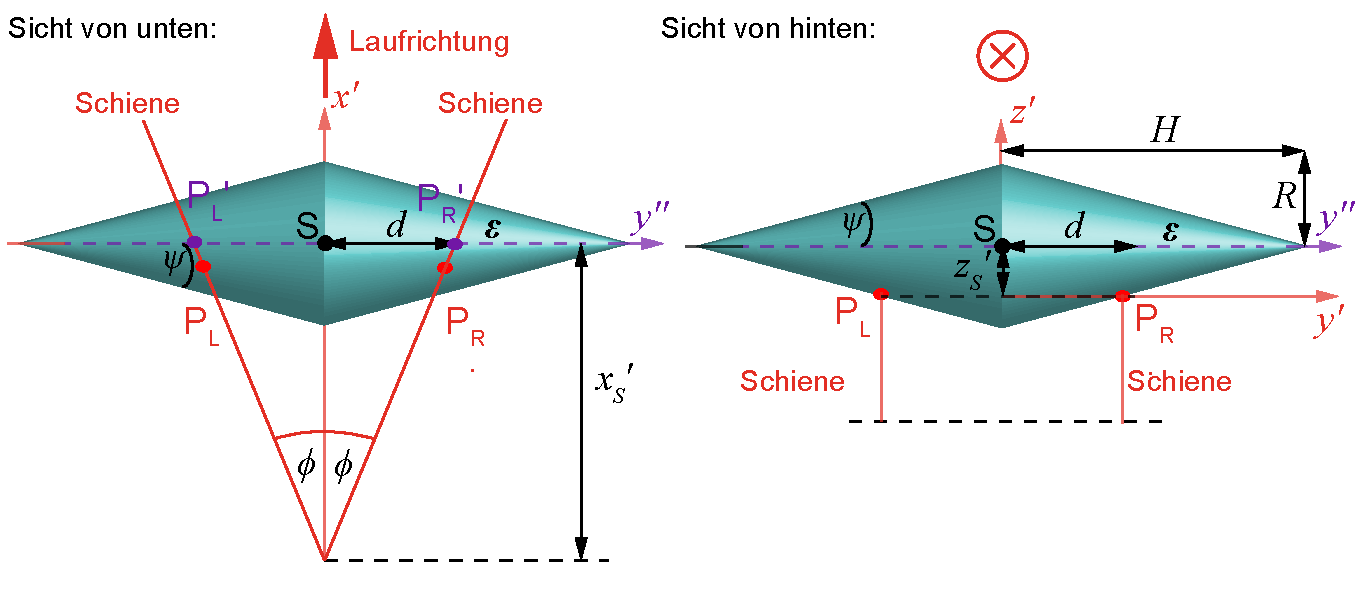
\includegraphics[width=\textwidth]{Doppelkegel02.pdf}
  \caption[Geometrie des aufw�rts laufenden Doppelkegels.]{Geometrie des aufw�rts laufenden Doppelkegels. Man beachte, dass wir zur (vorl�ufigen) Vereinfachung der Rechnung die realen Auflagepunkte $\text{P}_\text{L},~\text{P}_\text{R}$ n�herungsweise unter die Symmetrieachse $\vec{\epsilon}$ in die Punkte $\text{P}_\text{L}',~\text{P}_\text{R}'$ gelegt haben.} \label{abb:bew_doublecone02}
\end{figure}

Man liest aus \figref{bew_doublecone02}, in der das System schiefe Schienen und Doppelkegel im Schnitt von unten und von hinten ebenso wie die verwendeten Koordinatensysteme $\vec{\Sigma}, \vec{\Sigma}'$ dargestellt sind, die folgenden geometrischen Beziehungen f�r die Position des Schwerpunktes S im KOS $\vec{\Sigma}'$ ab:
        \begin{align}
            y_\text{S}' &= \frac{\D}{\tan\phi}\,, ~~~~x_\text{S}' = 0 \,~~~~z_\text{S}' = \lk H-d\rk\,\tan\psi = \lk R\cot\psi-d\rk\,\tan\psi\,,\nonumber \\
	          \rightarrow z_\text{S}' &= R-y_\text{S}'\,\tan\phi\,\tan\psi = - y_\text{S}'\tan\phi\,\tan\psi + H\tan\psi\,. \label{eq:bew_doublecone03} 
        \end{align}

Das ist eine lineare Funktion in $z_\text{S}' = z_\text{S}'(y_\text{S}')$, der Schwerpunkt bewegt sich also interessanterweise auf einer Geraden.
Wir haben bei der Herleitung von \eqref{eq:bew_doublecone03} allerdings die N�herung gemacht, dass der Auflagepunkt des Kegels auf den Schienen (der sogenannte Rollpunkt) direkt unter der Symmetrieachse des Doppelkegels liegt.
Wir werden diese Einschr�nkung sp�ter aufheben.\\ 
Gehen wir nun in das Koordinatensystem $\vec{\Sigma}$, das durch Drehung um den Anstiegswinkel $\theta$ um die gemeinsame $x=x'$-Achse aus $\vec{\Sigma}'$ hervorgeht (\figref{bew_doublecone01}). Wir erhalten\footnote{Da $x_\text{S}= x_\text{S}' = 0$, haben wir effektiv ein zweidimensionales System.}
        \begin{align}
            \begin{pmatrix}
                    y_\text{S} \\
                    z_\text{S}
            \end{pmatrix}
            &=
            \begin{pmatrix}
                    \cos\theta & -\sin\theta \\
                    \sin\theta & \cos\theta
            \end{pmatrix}
            \begin{pmatrix}
                    y_\text{S}' \\
                    z_\text{S}'
            \end{pmatrix}\,,\nonumber \\
            z_\text{S} &= y_\text{S}'\,\sin\theta + z_\text{S}'\,\cos\theta = y_\text{S}'\,\sin\theta +\lk R-y_\text{S}'\,\tan\phi\,\tan\psi\rk\,\cos\theta\,,\nonumber\\
            z_\text{S} &= y_\text{S}'\,\lk \sin\theta-\tan\phi\,\tan\psi\,\cos\theta\rk + R\,\cos\theta\,. \label{eq:bew_doublecone04}
        \end{align}
Wenn der Ausdruck in der Klammer negativ ist, dann wird $z_\text{S}$ mit zunehmendem $y_\text{S}'$ (also beim Aufrollen) kleiner, \dh der Schwerpunkt sinkt.
Eine Bedingung f�r das \glqq Aufw�rtsrollen\grqq{} ist also 
        \begin{align}
            \tan\theta \leq \tan\phi\,\tan\psi \,,\label{eq:bew_doublecone06}
        \end{align}
was eine geometrische Beziehung zwischen den drei Winkeln $\phi$ (halber �ffnungswinkel der Schienen), $\psi$ (halber Kegelwinkel) und $\theta$ (Schienenneigung) ist. 
Beim Aufw�rtsrollen wird also durch Absenken des Schwerpunktes um $\Delta z_\text{S}$
potentielle Energie in kinetische Energie der Translation und der Rotation umgewandelt.
Im Grenzfall, wenn nur noch die Kegelspitzen die Schienen ber�hren ($y_\text{S}'=H/\tan\phi$),
wird der Doppelkegel ausschlie�lich Rotationsenergie besitzen,
sodass wir folgende Energiebilanz aufschreiben k�nnen:
        \begin{align}
        \begin{split}
            \Delta T_\text{Rot} &= -\Delta U \, \rightarrow \frac{1}{2}\,J_\text{S}\,{\omega_\text{f}}^2 = -m\,g\,\Delta z_\text{S,f} \,. \label{eq:bew_doublecone07}
        \end{split}
        \end{align}
In \cite{Gallitto2011} wurden Experimente f�r einen homogenen Doppelkegel mit folgenden Werten angegeben:
        \begin{align*}
          \phi &= \SI{15.5}\degree\,, ~\theta = \SI{6.5}\degree\,, ~ \psi = \SI{24.78}\degree\,, ~ R = \SI{30}{\mm}\,, ~ H = \SI{65}{\mm}\,, ~M = \SI{122.5}{\g}\,.
          %R &= \SI{30}{\mm}\,, ~~~~ H = \SI{65}{\mm}\,, ~~~~ \varrho = \varrho_\text{Al}=\SI{2.7}{\g\per\cm\cubed}\,, ~~~~ M = \SI{122.5}{\g}\,,  ~~~~ ,.
        \end{align*}
F�r das Tr�gheitsmoment bezogen auf die Symmetrieachse des Doppelkegels ermittelt man
$J_\text{S} = \frac{3}{10}\,M\,R^2 = \SI{330.75}{\g\cm\squared}$.
Die finale Rotationsfrequenz $\omega_\text{f}$ ergibt sich
aus der H�hen�nderung $\Delta z_\text{S,f}$, die man aus geometrischen �berlegungen
zu $\Delta z_\text{S,f} \approx \SI{3}{\milli\metre}$ bestimmen kann.
Aus \eqref{eq:bew_doublecone07} folgt, dass die finale Rotationsfrequenz
$\omega_\text{f}$ beim homogenen Doppelkegel in etwa 
        \begin{align*}
            \omega_\text{f} = \sqrt{\frac{20g+\Delta z_\text{S,f}}{3R^2}} &\approx \SI{14.8}{\radian\per\second} \approx 2.3\,\text{Umdrehungen}\,\SI{}{\per\second}
        \end{align*}
betr�gt und interessanterweise nicht von der Masse abh�ngt.

\subparagraph{\textbf{Lagrange-Funktion und Lagrange-Gleichungen des Doppelkegels}}

Wir wollen uns nun der zeitlichen Dynamik zuwenden.
Wir folgen dabei den Betrachtungen in \cite{Gandhi2005}
und wollen den Lagrange-Formalismus benutzen.
Dabei ber�cksichtigen wir jetzt, dass die Kontaktpunkte $\text{P}_\text{L}$
\bzw $\text{P}_\text{R}$ von Schiene und Kegelmantel
nicht in der die Symmetrieachse des Kegels enthaltenden vertikalen Ebene liegen,
sondern vielmehr mit der Symmetrieachse eine Ebene bilden,
die die vertikale Ebene unter einem Winkel schneidet (\figref{bew_doublecone03}).%
\footnote{Die Situation eines rollenden Zylinders auf der V-f�rmigen Doppelschiene
ist anders als die des Doppelkegels.
Man macht sich leicht klar, dass beim Zylinder die Normale von der Rollfl�che
durch den Rollpunkt auch durch die Symmetrieachse $\epsilon$ geht,
nicht jedoch beim Doppelkegel.
Ein Doppelkegel, der auf parallelen Schienen abrollt,
h�tte daher auch dieselbe Abrollsituation wie ein Zylinder.}
Wir m�ssen daher zum Aufstellen der Lagrange-Funktion
die Lage der Kontaktpunkte relativ zum Schwerpunkt kennen. 
In \figref{bew_doublecone03} und \figref{bew_doublecone04} haben wir deshalb
die Geometrie genauer dargestellt, dabei zeigt in \figref{bew_doublecone04}
der Kreis den Querschnitt des Doppelkegels in seiner Schwerpunktebene an.
Die rote Linie ist die Schnittlinie der $x'$-$y'$-Ebene von $\vec{\Sigma}'$ mit einer Ebene,
die senkrecht zur Symmetrieachse des Doppelkegels steht.
$\text{P}$ ist der sogenannte virtuelle Kontaktpunkt.
Es wird sich als vorteilhaft erweisen, dass man zur Berechnung der Rotationsenergie
die Koordinaten des virtuellen Kontaktpunktes $\text{P}$ nutzt.
Es ergeben sich dadurch deutlich einfachere Beziehungen f�r die Rotationsenergie.

\begin{figure}
  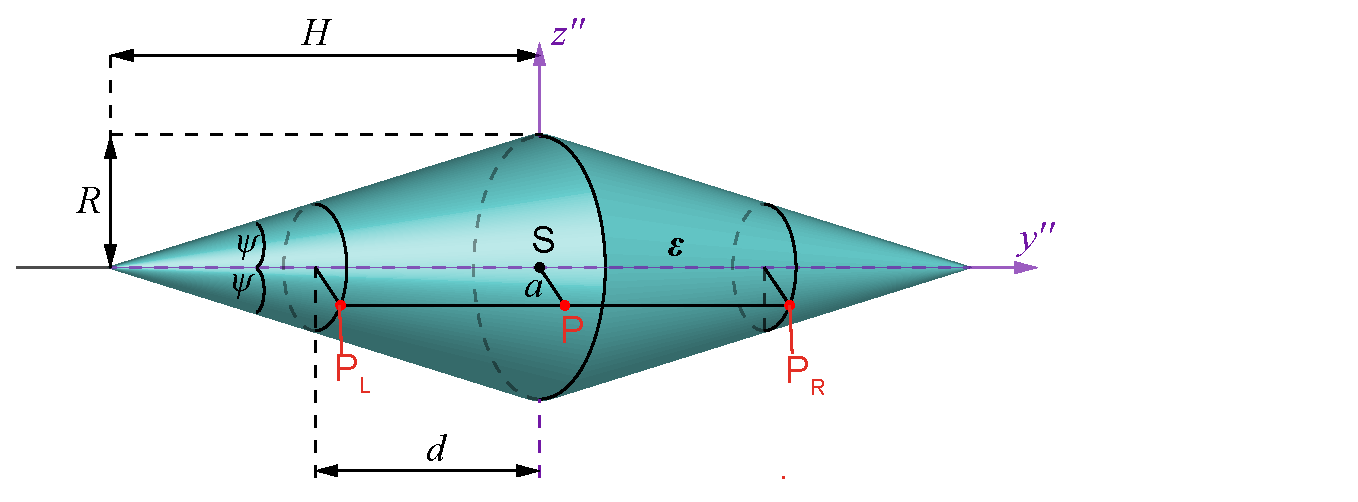
\includegraphics[width=\textwidth]{Doppelkegel03.pdf}
  \caption[Geometrie des Doppelkegels im mitbewegten KOS.]{Geometrie des Doppelkegels im mitbewegten KOS $\vec{\Sigma}''$. $\text{P}_\text{L}, \text{P}_\text{R}$ sind die realen Kontaktpunkte auf den Schienen. $\text{P}$ ist ein \anf{virtueller Kontaktpunkt} im Abstand $a$ vom Schwerpunkt $\text{S}$, $\psi$ ist der halbe �ffnungswinkel der Kegel.} \label{abb:bew_doublecone03}
\end{figure}

Wir werden daher als n�chstes die Koordinaten des Punktes P
als Funktion der Schwerpunktkoordinaten herleiten,
wobei sich der Punkt vom tats�chlichen Kontaktpunkt
nur in seiner $x''$-Koordinate unterscheidet \cite{Gandhi2005}. Daraus wird der
Winkel $\alpha = \alpha_\text{P}$ und die L�nge $a = a_\text{P}$ bestimmt, womit 
der Punkt P eindeutig charakterisiert ist. 
Zun�chst brauchen wir dazu den Normalenvektor $\vec{n}$ an einem Punkt $x'',y'',z''$
auf der Kegeloberfl�che und starten deshalb mit der Kegelgleichung f�r die Oberfl�che

        \begin{align*}
            f\lk x'',y'',z''\rk &= -\sqrt{\lk H-x''\rk^2\,\tan^2\psi -{y''}^2}-z'' = 0 \,,\\
            \vec{n}_\text{K} &= \vec{\nabla}f = \frac{1}{\sqrt{\lk H -x''\rk^2\,\tan^2\psi -{y''}^2}} \,
						\begin{pmatrix}
                    \lk H-x''\rk\,\tan^2\psi\\
                     y''\\
                    -\sqrt{\lk H-d\rk^2\,\tan^2\psi -{y''}^2}
            \end{pmatrix}\,.
        \end{align*}
Speziell f�r den Kontaktpunkt P gilt $y''=y_\text{P}''$ und $y'' = y_\text{P}'' = d$ und somit
        \begin{align}
            \vec{n}_\text{K,P} = \frac{1}{\sqrt{\lk H-d\rk^2\,\tan^2\psi -{y_\text{P}''}^2}}\,\begin{pmatrix}
                    \lk H-d\rk\,\tan^2\psi \\ y_\text{P}'' \\
                    -\sqrt{\lk H-d\rk^2\,\tan^2\psi -{y_\text{P}''}^2}
            \end{pmatrix}\,.
            \label{eq:bew_doublecone08}
        \end{align}
Der in Richtung der (rechten) Schiene zeigende Einheitsvektor ist gegeben durch 
        \begin{align}
            \vec{e}_\text{S} = 
            \begin{pmatrix}
                    \cos\phi\\
                    \sin\phi\\
                    0
            \end{pmatrix} 
            \label{eq:bew_doublecone09}
        \end{align}
und steht wegen der Rollbedingung tangential zur Kegeloberfl�che, \dh es gilt
        \begin{align}
            \vec{n}_\text{K,P}\cdot \vec{e}_\text{S} = 0\,. \label{eq:bew_doublecone10}
        \end{align}
Daraus k�nnen wir sofort $y_\text{P}''$ zu 
        \begin{align}
            y_\text{P}'' = -\lk H-d\rk\,\tan^2\psi\,\tan\phi \label{eq:bew_doublecone11}
        \end{align}
bestimmen. 

\begin{figure}
\begin{minipage}{\textwidth}
\leftfigure{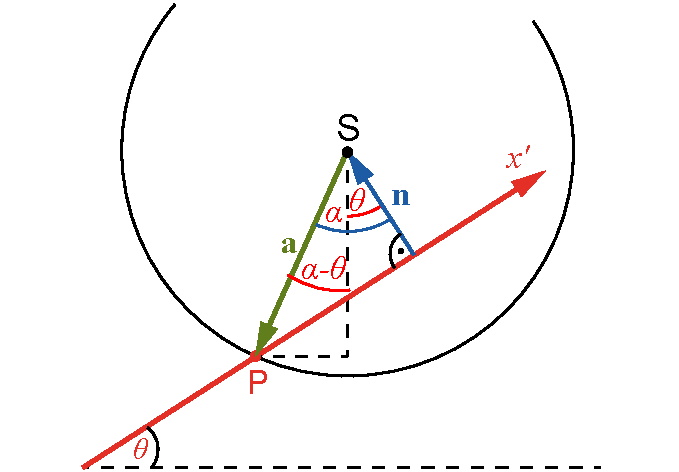
\includegraphics[width=0.5\textwidth]{Doppelkegel04.pdf}}%
\hspace{\fill}
\rightfigure{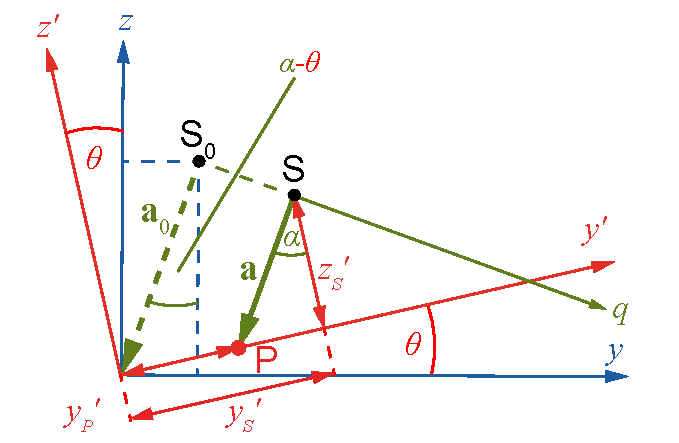
\includegraphics[width=0.5\textwidth]{Doppelkegel05a.pdf}}
\leftcaption[Lage des virtuellen Auflagepunktes beim Doppelkegel.]{Lage des virtuellen Auflagepunktes $\text{P}$ beim aufw�rts rollenden Doppelkegel im KOS $\vec{\Sigma}''$. Der Kreis ist der Querschnitt in der Mittelebene des Doppelkegels.} \label{abb:bew_doublecone04}
\rightcaption[Abstandsvektor und Schwerpunktskoordinaten.]{Beziehung zwischen dem Abstandsvektor $\vec{a}$ und den Schwerpunktskoordinaten ($y_\text{S}', z_\text{S}'$) im KOS $\vec{\Sigma}'$. Definition der generalisierten Koordinate $q$.} \label{abb:bew_doublecone05}
\end{minipage}
\end{figure}

\begin{figure}
  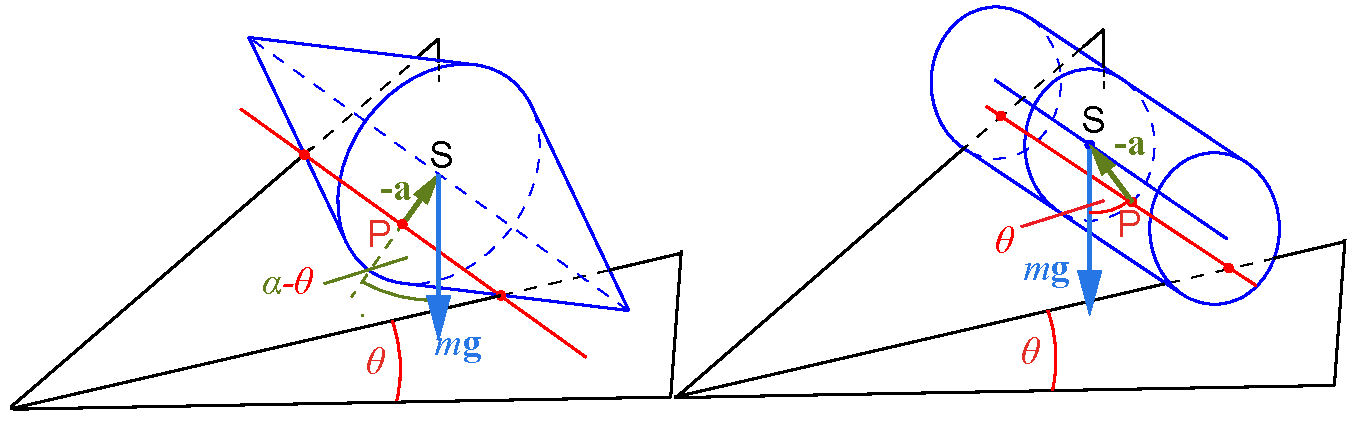
\includegraphics[width=\textwidth]{Doppelkegel04a.pdf}
  \caption[Vergleich der Drehmomente beim Doppelkegel und beim Zylinder.]{Vergleich der Drehmomente beim Doppelkegel und beim Zylinder.} \label{abb:bew_doublecone04a}
\end{figure}


Aus \figref{bew_doublecone04} erhalten wir andererseits
        \begin{align*}
            y_\text{P}'' &= -a\,\sin\alpha\,, 
        \end{align*}
woraus wir schlie�lich die gesuchten Gr��en $a$ und $\alpha$ erhalten:
        \begin{align}
            a= \lk H-d\rk\,\tan\psi ~~~~ \text{und} ~~~~ \sin\alpha = \tan\phi\,\tan\psi \,. \label{eq:bew_doublecone12}
        \end{align}
Der Winkel $\alpha$ ist damit vollst�ndig durch die Geometrie von Kegel und\,(!) Schienen festgelegt und konstant.
Wie man aus \figref{bew_doublecone04} und \figref{bew_doublecone04a}a erkennt, bestimmt der Winkel $\alpha-\theta$ die Gr��e des Drehmoments:
\begin{align}
	\MD = -\vec{a} \times m\vec{g}  = -\lk H-d\rk\,\tan\psi\,m\,g \sin(\alpha-\theta)\, \vecppeX \,. \label{eq:bew_doublecone12a}
\end{align}
Zeigt das Drehmoment in die negative $\vecppeX\,$-Richtung, rollt der Kegel in positive $\vecppeY$-Richtung, also \anf{aufw�rts}. Im Gegensatz dazu zeigt das resultierende Drehmoment beim Zylinder immer in positive Richtung $\vecppeX$, der Zylinder kann nur \anf{abw�rts} rollen (\figref{bew_doublecone04a}b).\\
Mit diesem Wissen k�nnen wir nun an die \anf{Konstruktion} der Lagrange-Funktion gehen. Zun�chst bestimmen wir in einem Koordinatensystem $\vec{\Sigma}'$ die Bewegung des Schwerpunktes als Funktion von $x_\text{P}'$ und $\alpha$. Aus \figref{bew_doublecone04} und \figref{bew_doublecone05} sowie \eqref{eq:bew_doublecone11} finden wir 
        \begin{align}
				    d &= y_\text{P}' \tan\phi\,, ~~ z_\text{S}' = a\,\cos\alpha \,, ~~ a= H\,\tan\psi - y_\text{P}'\,\sin\alpha \,,\nonumber \\
            \rightarrow z_\text{S}' &= \lk H\,\tan\psi - y_\text{P}'\,\sin\alpha\rk\,\cos\alpha\,,\\
						 \rightarrow y_\text{S}' &= y_\text{P}' + a\,\sin\alpha = H\,\tan\psi - y_\text{P}'\,\sin\alpha\,~~\text{und}~~ y_\text{P}' = \frac{y_\text{S}' - H\,\tan\psi\,\sin\alpha}{\cos^2\alpha}\,, \label{eq:bew_doublecone13}
        \end{align}
woraus schlie�lich
        \begin{align}
            z_\text{S}' = C\,y_\text{S}' + D ~~ \text{mit} ~~ C = -\tan\alpha ~~~ \text{und} ~~~ D = H\,\tan\psi\,\lk \cos\alpha-\tan\alpha\,\sin\alpha\rk \label{eq:bew_doublecone14}
        \end{align} 

folgt. Wir erhalten also wie in \eqref{eq:bew_doublecone03} wieder einen linearen Zusammenhang wie zwischen $z_\text{S}'$ und $y_\text{S}'$, allerdings mit einigen Unterschieden. Diese resultieren aus der bei der Herleitung von \eqref{eq:bew_doublecone03} gemachten N�herung bez�glich des Rollpunktes.%
\footnote{F�r kleine Winkel $\alpha, \psi$ geht \eqref{eq:bew_doublecone14} in \eqref{eq:bew_doublecone03} �ber.}
Die Erkl�rung daf�r, dass der Schwerpunkt sich auf einer Geraden bewegt,
ist physikalisch recht einleuchtend.
Da die Bewegung des Doppelkegels aus einer �berlagerten Translation ($\vec{v}_\text{trans,S}$)
und Rotation ($\vec{v}_\text{rot}$) besteht, muss f�r die Rollpunkte
$\text{P}_\text{L},\,\text{P}_\text{R}$ und somit auch P gelten:%
\footnote{Wenn die Translationsgeschwindigkeit gleich dem momentanen Radius zum Kontaktpunkt mal der Winkelgeschwindigkeit ist, dann bleibt der Punkt $P$ in Ruhe, \dh wir haben Rollen ohne Gleiten.}  
	\[\vec{v}_\text{rot}=-\vec{v}_\text{trans,S}\,~~\text{und}~~\vec{a}\,\bot\,\vec{v}_\text{trans,S}\,.
\]
Da der Vektor $\vec{a}$ konstant ist und wegen der Symmetrie $x_\text{S} = 0$ gilt, muss $z_\text{S}(y_\text{S})$ eine Gerade sein.\\

F�r die Lagrange-Funktion f�hren wir nun mit \eqref{eq:bew_doublecone14} eine neue generalisierte Koordinate $q$ ein \cite{Gandhi2005}, die sich aus der Distanz des Schwerpunktes auf seiner Bewegungsgeraden vom Startpunkt $y_\text{S0}'$ ergibt (\figref{bew_doublecone05}):
        \begin{align}
            y_\text{S}' &= y_\text{S0}' + q\,\cos\alpha\,, ~~\text{bzw.}~~ q = \frac{y_\text{S}'-y_\text{S0}'}{\cos\alpha}\label{eq:bew_doublecone15} \\
           \text{mit} ~~ y_\text{S0}' &= a_0\,\sin\alpha = R\,\sin\alpha = H\,\tan\psi\,\sin\alpha = H\,\tan^2\psi\,\tan\phi \nonumber \,.
        \end{align}
Daraus erhalten wir mit \eqref{eq:bew_doublecone13} die einfache Beziehung
        \begin{align}
            a(q) = H\,\tan\psi -q\,\tan\alpha\,. \label{eq:bew_doublecone16}
        \end{align}
        Die Rollbedingung lautet dann
        \begin{align*}
            \omega &= -\frac{\dot{q}}{a\lk q\rk} = -\frac{\dot{q}}{H\,\tan\psi - q\,\tan\alpha}\,.
        \end{align*}
Wir f�hren f�r die numerischen Rechnungen zweckm��ige Abk�rzungen $C_1 \ldots C_3$ f�r konstante Gr��en ein 
        \begin{align*}
  C_1 &= \frac{3R^2}{10\tan^2\alpha}\,,~~~C_2 = -g\,\sin(\alpha-\theta)\,,\\
	C_3 &= H\,\frac{\tan\psi}{\tan\alpha}\,~~ \text{und}~~ p(q) = C_3 - q\,.
        \end{align*}   
und erhalten damit die kinetische Energie f�r den homogenen Doppelkegel in relativ kompakter Form zu
        \begin{align}
            T(q, \dot{q}) &= \frac{1}{2}\,M\,\dot{q}^2+\frac{1}{2}\,J_\text{S}\,\omega^2 = \frac{1}{2}\,\dot{q}^2\,M\,\lk 1+\frac{3R^2}{10}\,\frac{1}{\lk H\,\tan\psi -q\,\tan\alpha\rk^2}\rk  \nonumber \\
						&= M\,\frac{1}{2}\,\dot{q}^2\,\lk 1+\frac{C_1}{\lk C_3 - q\rk^2}\rk\,. \label{eq:bew_doublecone17}
	\end{align}
F�r die potentielle Energie m�ssen wir wieder in das $\vec{\Sigma}$ -KOS gehen und erhalten (siehe auch \figref{bew_doublecone04})
        \begin{align}
            U = -m\,g\,q\,\sin\lk\alpha-\theta\rk = m\,C_2\,q\,. \label{eq:bew_doublecone18}
        \end{align}
Hieraus leitet sich wieder die Bedingung f�r das Aufw�rtsrollen ab, n�mlich 
        \begin{align}
            \sin\lk\alpha-\theta\rk &> 0 ~~\Leftrightarrow~~\sin\alpha\,\cos\theta -\cos\alpha\,\sin\theta > 0 ~~\text{\bzw} \nonumber \\
						\tan\theta &< \frac{\tan\phi\,\tan\psi}{\sqrt{1-\tan^2\phi\,\tan^2\psi}}\,. \label{eq:bew_doubleconeCondition}
        \end{align}
Dies geht f�r kleine Winkel, bei denen die Kontaktpunkte nahezu unter der Symmetrieachse liegen,
wieder in die bereits bekannte N�herung \eqref{eq:bew_doublecone06} �ber. 
Man k�nnte beim Blick auf \eqref{eq:bew_doublecone17} vermuten,
dass $T(q, \dot{q})$ f�r $q \rightarrow C_3 = H\,\tan\psi/\tan\alpha $ divergiert.
Das ist aber nicht der Fall, da auch $\lim\limits_{q \to C_3} \dot{q} = 0$ gilt,
wie man leicht �berpr�fen kann. \\
Aus der durch $m$ dividierten Lagrange-Funktion $\hat{\mathcal{L}} = (T-U)/m$ folgt die Bewegungsgleichung f�r $q$,
	\begin{align}
  \ddot{q} & = -\frac{C_1}{p(q)\,(p(q)^2+C_1)}\, \dot{q}^2 - \frac{C_2\,p(q)^2}{p(q)^2+C_1}\,, \label{eq:bew_doubleconeLGL}
	\end{align}
die eine nichtlineare Gleichung darstellt, die wir mit \odevf{} in MATLAB numerisch integrieren. 
% Eventuell Darstellung der Nebenrechnung
%\begin{nebenrechnung}{Nebenrechnung:}
%\begin{align*}
    %\hat{\mathcal{L}} = \frac{\mathcal{L}}{M} = \underbrace{ \frac{1}{2}\,\dot{q}^2\,\lek 1+ \frac{C_1}{\lk C_3-q\rk^2}\rek}_{\substack{T}}  - 
%\underbrace{C_2\,q }_{\substack{U}}
%\end{align*}
%\begin{align*}
    %\frac{\D}{\D t}\, \frac{\d \hat{\mathcal{L}}}{\d \dot{q}} &= \ddot{q}\, \underbrace{\lek 1 + \frac{C_1}{\lk C_3-q\rk^2}\rek}_{Q} + \dot{q}\,\frac{\D}{\D t}\,\frac{C_1}{\lk C_3-q\rk^2} 
    %= \ddot{q}\,Q + \frac{2C_1}{\lk C_3-q\rk^3}\,\dot{q}^2 \\
    %\frac{\d \hat{\mathcal{L}}}{\d q} &= \frac{1}{2}\,\dot{q}^2\,\frac{C_1\,\lk -2\rk\lk -1\rk}{\lk C_3-q\rk^3}+C_2 = \frac{C_1}{\lk C_3-q\rk^3}\,\dot{q}^2-C_2 \\
    %0 & = \frac{\d }{\d t}\, \frac{\d \hat{\mathcal{L}}}{\d \dot{q}} -  \frac{\d \hat{\mathcal{L}}}{\d q} = \ddot{q}\,Q + \frac{2C_1}{\lk C_3-q\rk^3}\,\dot{q}^2 - \frac{C_1}{\lk C_3-q\rk^3}\,\dot{q}^2 +C_2 \\
 %C_3-q &= p ~~~\rightarrow ~~  0 = \frac{p^2 + C_1}{p^2}\,\ddot{q} + \frac{C_1}{p^3}\,\dot{q}^2 + C_2 
%\end{align*}
%\end{nebenrechnung}
Alternativ zur Lagrange-Gleichung kann man nat�rlich auch unter Ber�cksichtigung der Energieerhaltung aus \eqref{eq:bew_doublecone17} und \eqref{eq:bew_doublecone18} mit $E_0 = T + U = U(q_0)$ die Variable $\dot{q}$ als Funktion von $q$ darstellen,
	\begin{align}
		\dot{q}= \pm \sqrt{\frac{2\lk E_0 + m\, g\, \sin(\alpha-\theta) \rk}{m+ J_\text{S}/\lk H\,\tan\psi - q\,\tan\alpha \rk^2}} = F(q)\,, \label{eq:bew_doublecone20}
	\end{align}
und somit $\dot{q}=\dot{q}(q) = \dot{q}(y)$ berechnen. Wie man an \eqref{eq:bew_doublecone20} erkennt, ist $\lim\limits_{q \to C_3} \dot{q} = 0$, was unsere Aussage best�tigt, dass zum Ende der Bewegung keine Translationsenergie mehr vorhanden ist (vgl.\ \figref{bew_doublecone06}). �ber Trennung der Variablen erhalten wir aus \eqref{eq:bew_doublecone20}
	\begin{align}
			t + C = \int\limits_{0}^{t} \D\,t' =  \int\limits_{0}^{q} F(q') \D\,q' \,. \label{eq:bew_doublecone21}
	\end{align}
Dieses Integral ist ebenfalls numerisch l�sbar und wir erhalten die inverse Funktion $t(q)$, aus der wir die gesuchte Funktion $q(t)$ bestimmen k�nnen.\\
Das Ergebnis $\dot{q}(q)$, sowie $T_\text{Trans}\lk q\rk$ und $T_\text{Rot}\lk q\rk$ \bzw $f_\text{pot}\lk q\rk$ sind in \figref{bew_doublecone06} zu sehen
(siehe \mscre \mlbewref{Doppelkegel01.m} bis \mlbewref{Doppelkegel04.m}).
�ber \eqref{eq:bew_doublecone15} ist $q$ mit $y_\text{S}'$ und $y_\text{S}'$ wiederum �ber \eqref{eq:bew_doublecone03} mit $y_\text{S}$ verkn�pft.
Diese messbaren Gr��en sind als $z_\text{S}(y_\text{S})$ \bzw $y_\text{S}(t)$ und $z_\text{S}(t)$ in \figref{bew_doublecone07} dargestellt.

\begin{figure}
  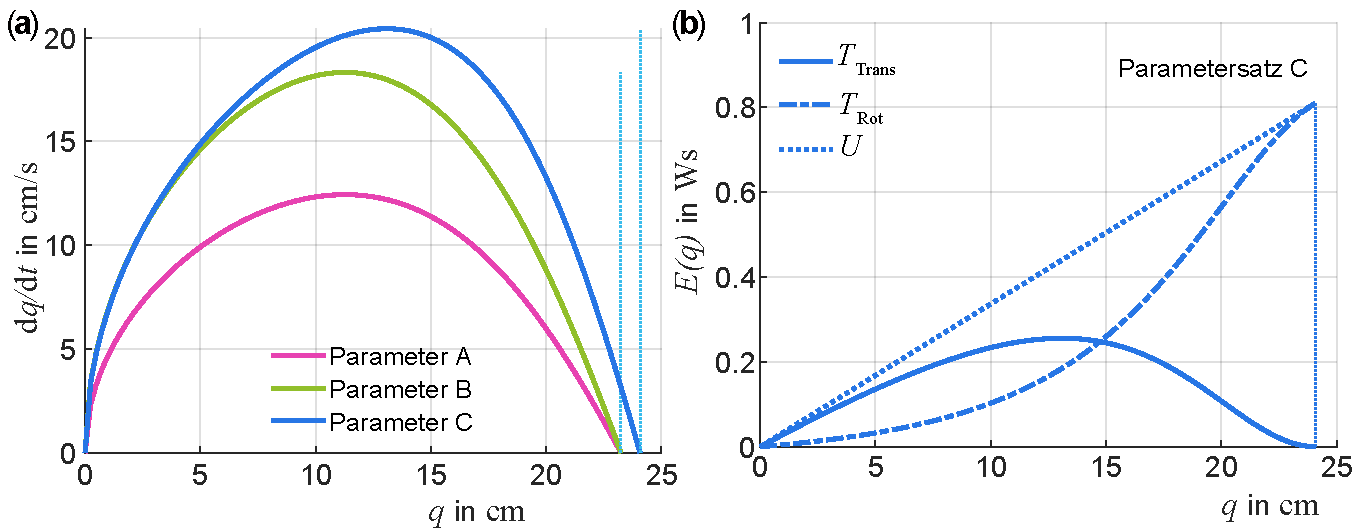
\includegraphics[width=\textwidth]{Doppelkegel06.pdf}
  \caption[Phasenraum und Energieanteile des aufw�rts laufenden Doppelkegels.]{\fa Phasenraum und \fb Energieanteile des aufw�rts laufenden Doppelkegels als Funktion der generalisierten Koordinate $q$. Parameter A: $\phi=15.5\degree,\, \theta=6.5\degree\,, J=\SI{330.75}{\g\cm\squared}$,\, B: $\phi=15.5\degree,\, \theta=5.5\degree,\, J=\SI{330.75}{\g\cm\squared}$,\,  C: $\phi=15.0\degree,\, \theta=5.5\degree,\, J=\SI{165.75}{\g\cm\squared}$. Sonstige Parameter: $H=\SI{6.5}{\cm},\, \psi=24.8\degree,\, M=\SI{122.5}{\g}$. Siehe auch \mscr{} \mlbewref{Doppelkegel04.m}.} \label{abb:bew_doublecone06}
\end{figure}

\begin{figure}
  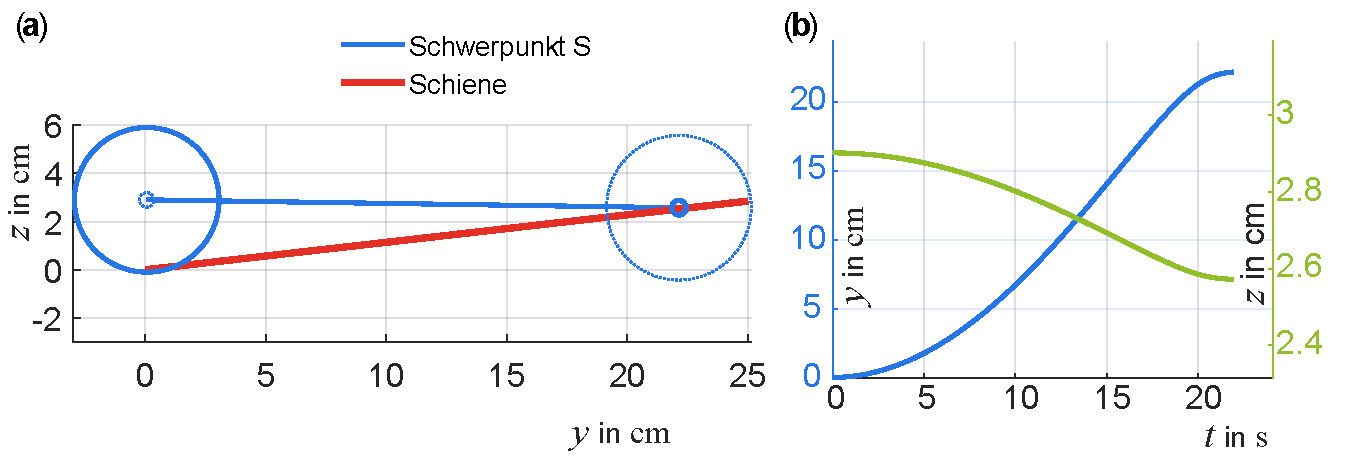
\includegraphics[width=\textwidth]{Doppelkegel07.pdf}
  \caption[Dynamik des aufw�rts laufenden Doppelkegels.]{Dynamik des aufw�rts laufenden Doppelkegels in kartesischen Koordinaten $y, z$. Siehe auch \mscr{} \mlbewref{Doppelkegel02.m}.} \label{abb:bew_doublecone07}
\end{figure}

Wir wollen noch darauf hinweisen, dass sich in der Literatur an verschiedenen Stellen leicht andere Formeln finden, die im Allgemeinen aus der unterschiedlichen Definition des Rollpunktes resultieren. In \probref{bew_doubleconecomp} vergleichen wir die Ergebnisse der verschiedenen Ans�tze miteinander.

\newpage

\subsubsection{Stabilit�t von Schienenfahrzeugen mit starren Achsen} \label{kap:bew_traintracks} 

Die im vorgehenden Kapitel behandelte Physik des Doppelkegels
hat eine ganz konkrete Anwendung in der Eisenbahntechnik gefunden.
Wer sich die Eisenbahnr�der genau anschaut (\figref{bew_TrainWheel01}), wird erkennen,
dass das Profil der R�der einem Ausschnitt aus einem Doppelkegel �hnelt.
Dieses Profil hat einen positiven Einfluss auf die Stabilit�t von Schienenfahrzeugen
entlang der Bewegung eines Gleises, bei der es stets zu unvermeidbaren lateralen St�rungen kommt.
Die Frage nach der Stabilit�t von Z�gen auf Gleisen mag nicht offensichtlich erscheinen. Vielfach h�rt man die falsche Erkl�rung, dass die erstaunliche Stabilit�t
eines kilometerlangen Zuges, der auf einem nur $\SI{1435}{\mm}$ breiten Gleis f�hrt,
durch den Radkranz/Flansch (\figref{bew_TrainWheel01} und \figref{bew_TrainWheel02}) zustandekommt. M�glicherweise brachte seshalb sogar Feynman\footnote{Richard Feynman (1918--1988) war ein US-amerikanischer Physiker und gilt als einer der gro�en Physiker des 20.\ Jahrhunderts, der wesentliche Beitr�ge zum Verst�ndnis der Quantentheorie geliefert hat. 1965  erhielt er 1965 den Nobelpreis f�r seine Arbeiten zur Quantenelektrodynamik. Feynman war es �beraus wichtig, die Gesetzm��igkeiten der Physik anschaulich und verst�ndlich Studenten und auch Laien nahezubringen.}\indexp{Feynman, Richard} das Thema in den 1970er Jahren (\url{https://www.youtube.com/watch?v=y7h4OtFDnYE}) in die popul�re Physik ein.
Tats�chlich zeigt die genauere Betrachtung, dass bei Rad-Schiene-Systemen
mit starr gekoppelten Achsen konisch profilierte R�der benutzt werden.
Da bei einem solchen Radsatz \zb bei Kurvenfahrten die Rollradien der beiden R�der
unterschiedlich gro� sind, die R�der sich aber gleich schnell drehen,
vollf�hrt das Rad mit dem gr��eren Rollradius einen l�ngeren Weg nach vorne
als das Rad mit dem kleineren Rollradius.
Daher lenkt ein zu weit links stehender Radsatz nach rechts und umgekehrt.
Hierdurch kommt es zu einer Art Schlingerbewegung, die wir
mit einer (r�umlichen) Differentialgleichung beschreiben k�nnen.
Im Grenzfall kleiner Abweichungen (Linearisierung) erh�lt man die in \figref{bew_TrainWheel03} dargestellte Sinuskurve, 
die erstmalig 1883 von Johannes Klingel\footnote{Johannes Klingel war ein Baurat und Ingenieur, der \ua an der Polytechnischen Hochschule Karlsruhe wirkte.}\indexp{Klingel, Johannes} an der damaligen Hochschule Karlsruhe ver�ffentlicht wurde.
Wir wollen in diesem Kapitel diese sogenannte Klingel-Formel herleiten
und brauchen die dabei wirkenden Kr�fte zun�chst nicht zu ber�cksichtigen,
sondern leiten den Sinuslauf aus einfachen geometrisch-kinematischen �berlegungen ab. 
Wir betrachten dazu \figref{bew_TrainWheel04}, die den Radk�rper schematisch als Doppelkegel von hinten zeigt und zwar in Normallage (gelb) und durch eine seitliche St�rung leicht nach links verschoben (blau).

\begin{figure}
\begin{minipage}{\textwidth}
\leftfigure{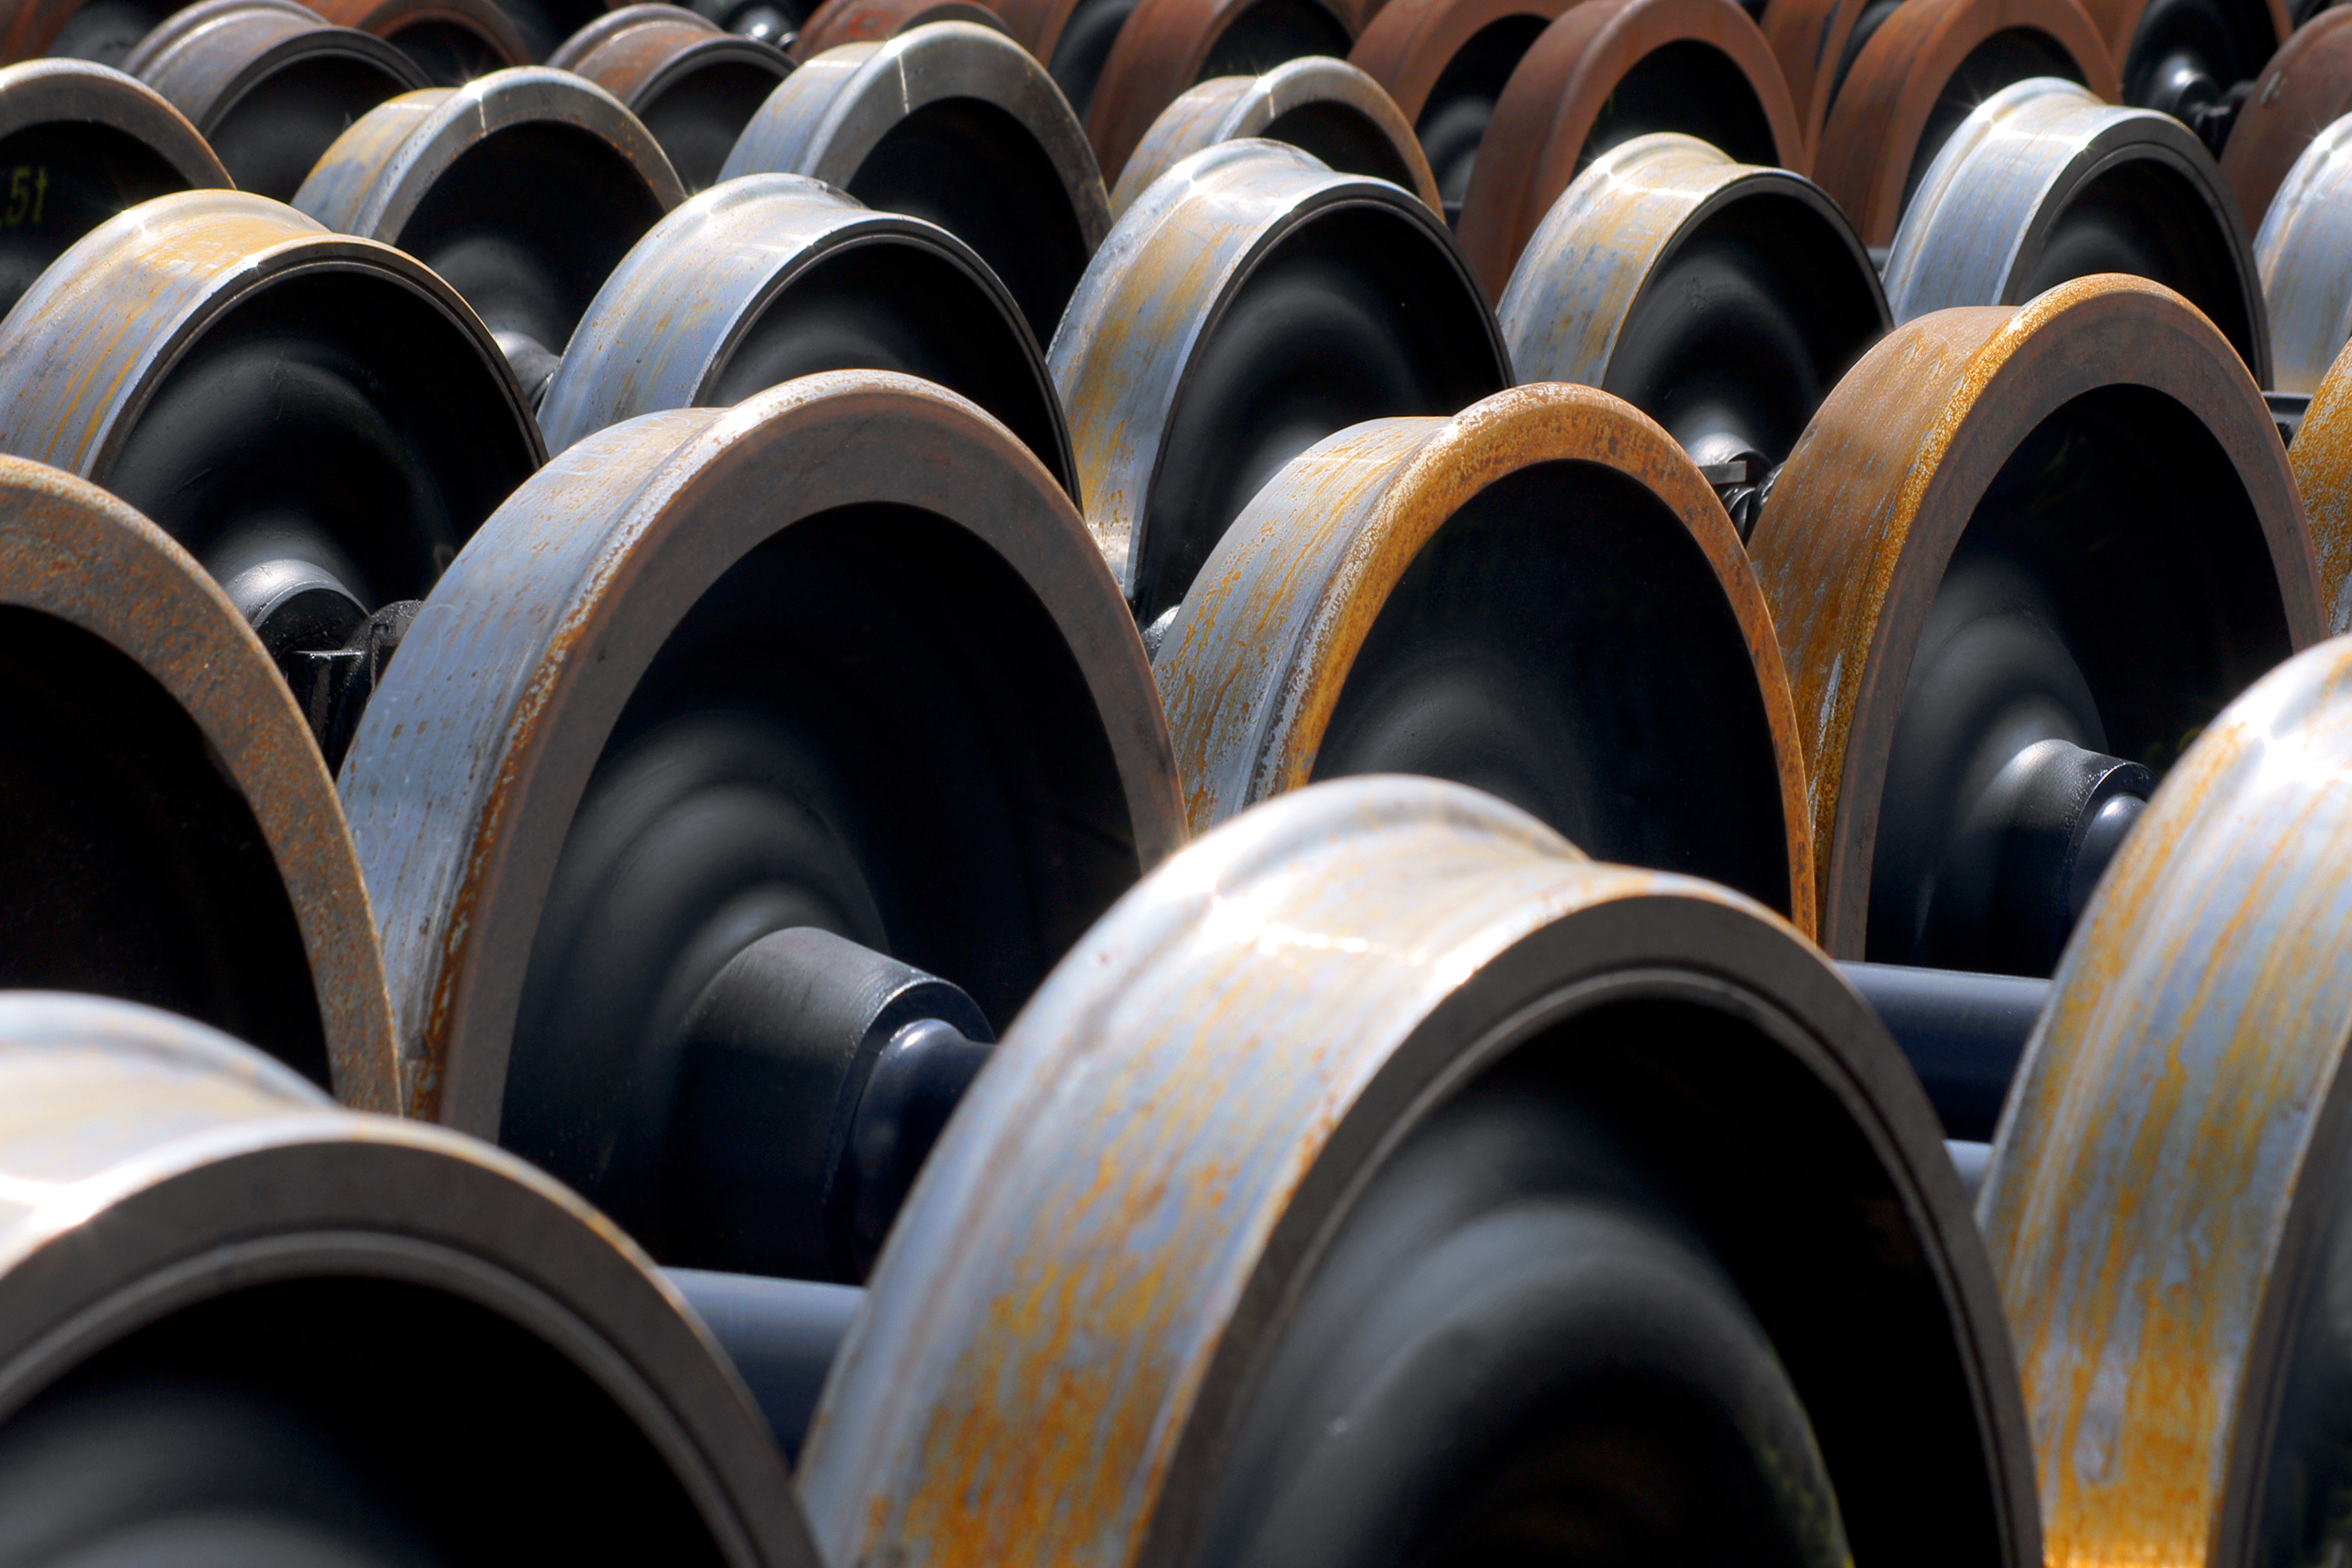
\includegraphics[width=0.4\textwidth]{TrainWheel.jpeg}}%
\hspace{\fill}
\rightfigure{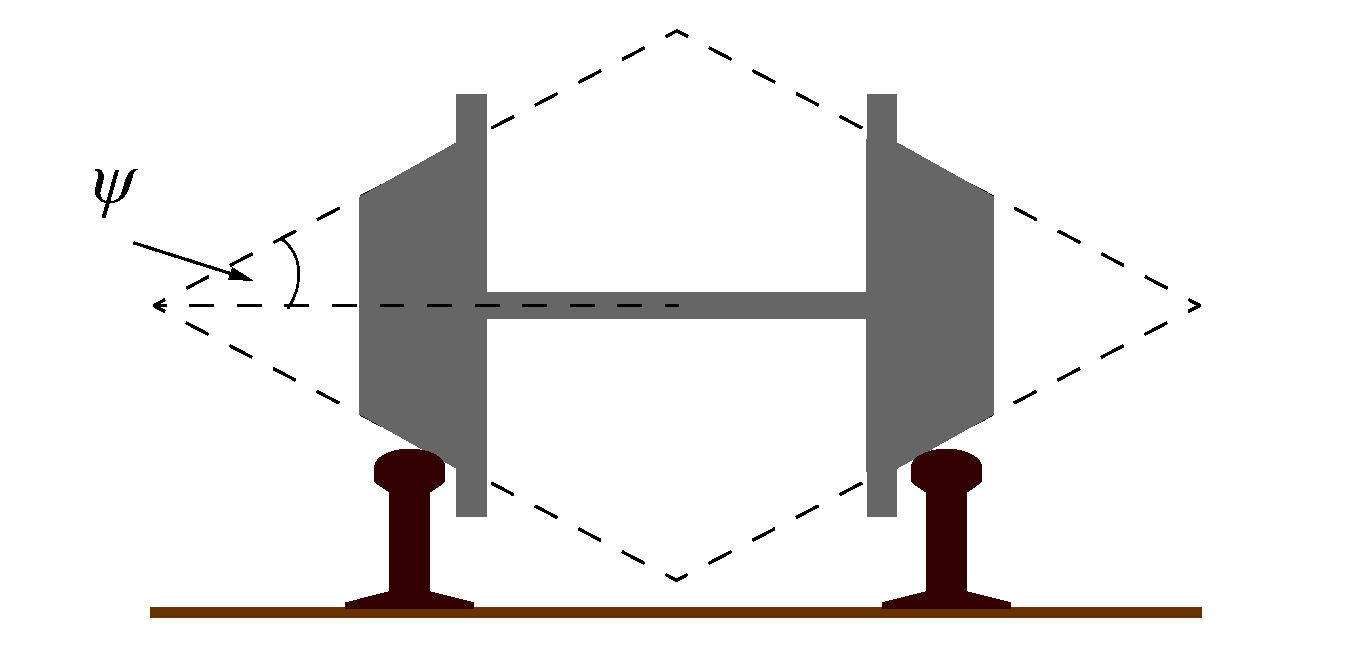
\includegraphics[width=0.6\textwidth]{WaggonAchse.pdf}}
\leftcaption{Eisenbahnr�der.} \label{abb:bew_TrainWheel01}
\rightcaption[Schematische Darstellung eines Eisenbahnachse auf einer Schiene.]{Schematische Darstellung eines Eisenbahnachse auf einer Schiene durch einen Doppelkegel. Der Winkel $\psi$ ist stark �berh�ht gezeichnet. In der Realit�t betr�gt er weniger als $0.05\,\text{rad} \approx 2.865\degree$.}\label{abb:bew_TrainWheel02}
\end{minipage}
\end{figure}

\begin{figure}
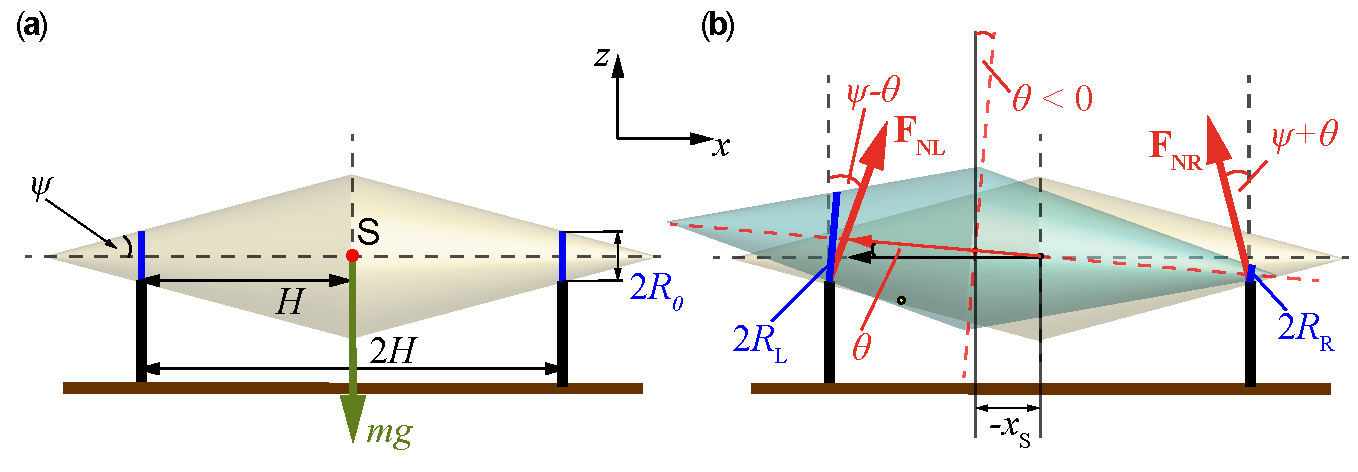
\includegraphics[width=\textwidth]{LateraleStoerung.pdf}%
\caption[Laterale St�rungen auf eine Radachse auf einer Doppelschiene.]{Laterale St�rungen auf eine Radachse auf einer Doppelschiene (Modellansicht von hinten in Fahrtrichtung). \fa Normallage der Radachse, $2H$ ist die Spurbreite, $\psi$ die Konizit�t der Radform, $R_0$ ist der Rollradius in der Normallage und S der Schwerpunkt der Achse, $m$ die Gesamtmasse von Achse und Achslast. \fb Lage bei lateraler St�rung und wirkende Normalkr�fte. $x_\text{S}$ ist die laterale Verschiebung des Schwerpunktes, $\theta$ der resultierende Kippwinkel aufgrund der Konizit�t, $\vec{F}_\text{N}$ die von der Schienenauflage ausgehenden Normalkr�fte und $R_\text{L}, R_\text{R}$ die neuen resultierenden Rollradien auf dem linken \bzw rechten Auflagepunkt. Der Winkel $\theta$ ist im eingezeichneten Fall negativ.} \label{abb:bew_TrainWheel04}
\end{figure}

    Wir starten von \figref{bew_TrainTrack01}. Als Parameter haben wir den Rollradius $R$, den Radstand $2H$ und die Konizit�t $\psi$. In der Normallage ist der Rollradius $R_0$ durch 
    \begin{align}
        R_0\,\omega_0 = v_0 \,\label{eq:bew_TrainTrack01}
    \end{align}
    mit der Vorw�rtsgeschwindigkeit $v_0$ des Schwerpunktes verbunden, $\omega_0$ ist die Rotationsgeschwindigkeit der Radachse. F�r den lateralen Versatz gilt entsprechend:
    \begin{align}
    \begin{split}
        R_\text{L}\,\omega_0 &= v_\text{L} \,,\\
        R_\text{R}\,\omega_0 &= v_\text{R} \,. 
    \end{split}\label{eq:bew_TrainTrack02}
    \end{align}
%
\begin{figure}
  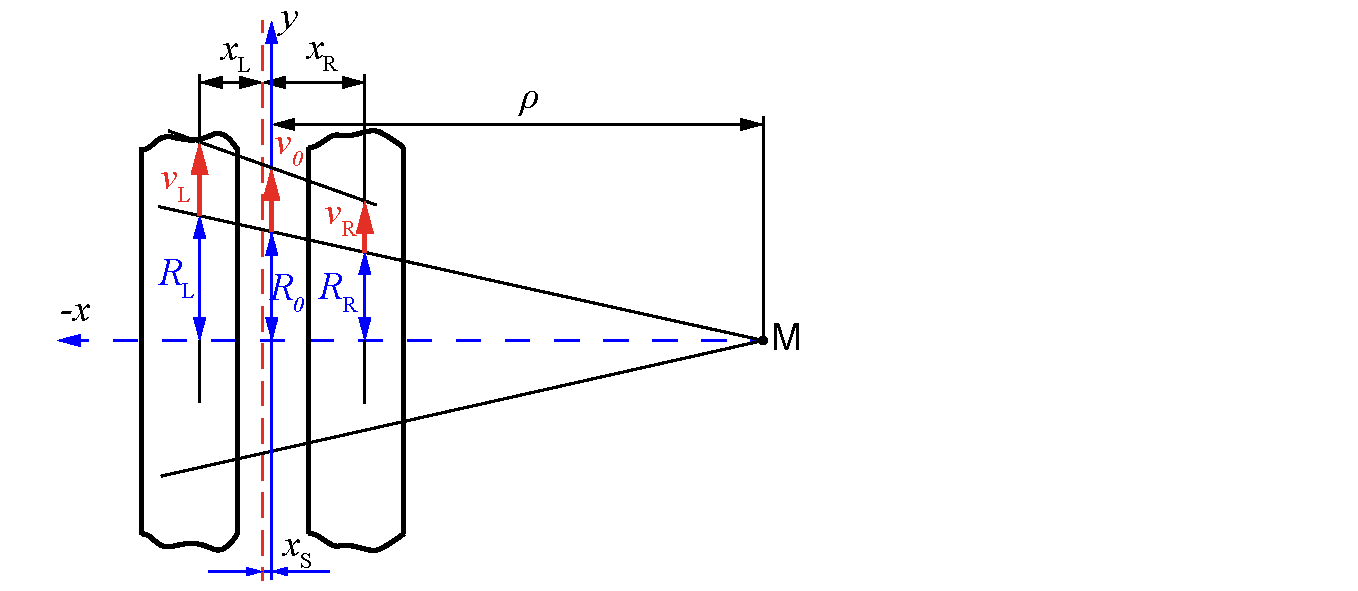
\includegraphics[width=\textwidth]{TrainTrack01.pdf}
  \caption[Kinematische Ableitung der Klingel-Formel.]{Kinematische Ableitung der Klingel-Formel.} \label{abb:bew_TrainTrack01}
\end{figure}
%
    �ber den Strahlensatz l�sst sich aus \figref{bew_TrainTrack01} \bzw \figref{bew_TrainWheel04} direkt ablesen:
    \begin{align}
        \frac{R_0}{\rho\lk x_\text{S} \rk} = \frac{R_\text{L}\lk x_\text{S}\rk - R_\text{R}\lk x_\text{S}\rk}{x_\text{L} + x_\text{R}} \,. \label{eq:bew_TrainTrack03}
    \end{align}
    Wir brauchen also die Differenz der Rollradien und die Gr��e $x_\text{L} + x_\text{R}$. Aus \figref{bew_TrainTrack01} kann man ableiten:
    \begin{align*}
        R_\text{L}-R_0 &\approx x_\text{S}\,\tan\psi\,, \\
        R_\text{R} - R_0 &\approx -x_\text{S}\,\tan\psi 
    \end{align*}
    und
    \begin{align*}
        x_\text{L} + x_\text{R} &\approx 2H\,.
    \end{align*}
    Damit ergibt sich, wenn man mit $\rho \lk x_\text{S} \rk$ als Kr�mmungsradius der Achsenlage ($y$ ist die Fahrtrichtung, $x$ die laterale Dimension) die Beziehung $1/\rho \lk x \rk \approx -\D^2 x_\text{S} / \D y^2$ in \eqref{eq:bew_TrainTrack03} einsetzt:
    \begin{align}
        \frac{\D^2x_\text{S}}{\D y^2} + \frac{\Delta R\lk x\rk}{R_0\,\lk x_\text{L}+ x_\text{R}\rk} = 0\,. \label{eq:bew_TrainTrack04}
    \end{align}
    Das ist schon die Klingel-Formel in ihrer allgemeinen Form (mit Annahme kleiner Winkel und Verschiebungen).\\
    F�r die konische Radform (Doppelkegel-Modell) k�nnen wir die Funktionen $\Delta R\lk x\rk = R_\text{L} -R_\text{R}$ und $\Delta x = x_\text{L} + x_\text{R}$ aufschreiben. %
    Aus \figref{bew_TrainTrack01} kann man ablesen:
    \begin{align}
    \begin{split}
        \left.\begin{aligned}
    	R_\text{L} &\approx R_0 + x_\text{S}\,\tan\psi\\
	    R_\text{R} &\approx R_0 - x_\text{S}\,\tan\psi
	        \end{aligned}
	\right\}
    \quad R_\text{L} - R_\text{R} \approx 2x_\text{S}\,\tan\psi
    \end{split}  \label{eq:bew_TrainTrack05}
    \end{align}
    und 
    \begin{align*}
        x_\text{L} + x_\text{R} &\approx 2H\,.
    \end{align*}
    Damit ergibt sich im Fall des Doppelkegel-Modells f�r die Klingel-Formel
    \begin{align}
        \frac{\D^2x_\text{S}}{\D y^2} +\frac{\psi}{R_0\,H} x_\text{S} = 0  \label{eq:bew_TrainTrack06}
    \end{align}
    und daraus die Wellenl�nge und Frequenz des Sinuslaufs zu 
    \begin{align}
    \begin{split}
        \Lambda_\text{K} &= 2\pi\,\sqrt{\frac{H\,R_0}{\psi}} \,, ~~~ f_\text{K} = \frac{v_0}{2\pi}\,\sqrt{\frac{\psi}{H\,R_0}}\,.
    \end{split} \label{eq:bew_TrainTrack07}
    \end{align}
		Die Gr��e $f_\text{K}$, manchmal auch Klingel-Frequenz genannt, charakterisiert also den sogenannten Sinuslauf (oder Wellenlauf) \cite{Knothe2003}. Die Bewegung ist bei kleinen Amplituden sinusf�rmig und hat eine konstante Wellenl�nge, daher also eine mit der Fahrgeschwindigkeit zunehmende Frequenz (\figref{bew_TrainWheel03a}).

\begin{figure}
  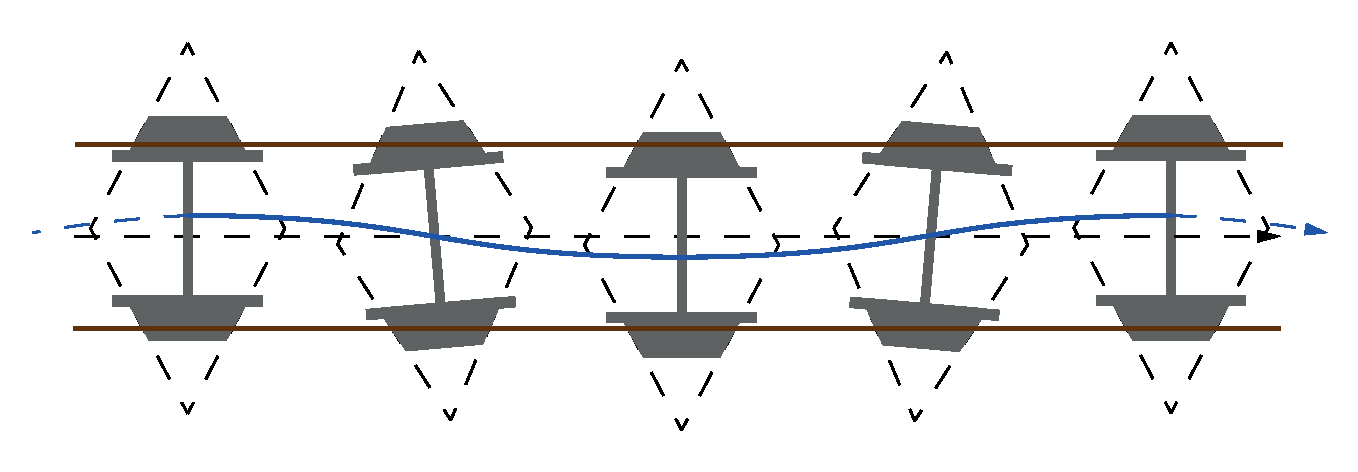
\includegraphics[width=\textwidth]{SinusLauf.pdf}
  \caption[Sinuslauf bei Z�gen mit starrer Achse.]{Sinuslauf bei Z�gen mit starrer Achse (Sicht von oben).} \label{abb:bew_TrainWheel03}
\end{figure}

\begin{figure}
  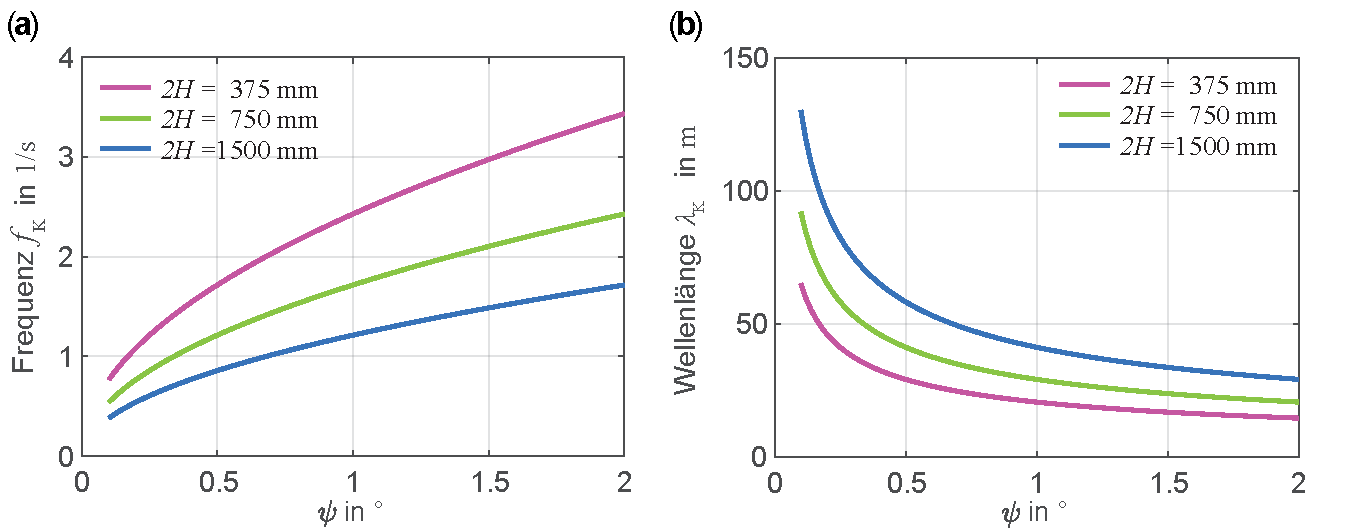
\includegraphics[width=\textwidth]{KlingelFrequenz.pdf}
  \caption[Frequenz und Wellenl�nge des Sinuslaufs als Funktion der Konizit�t.]{\fa Frequenz und \fb Wellenl�nge des Sinuslaufs als Funktion der Konizit�t. Vorw�rtsgeschwindigkeit $v_0 = \SI{50}{\metre\per\second}$.} \label{abb:bew_TrainWheel03a}
\end{figure}

In \probref{bew_TrainTrack} wollen wir uns das Rad-Schiene-System bei lateralen St�rungen dynamisch anschauen und uns auch den Fall anschauen, der eintritt, wenn das System \zb durch einen Lenkfehler gest�rt wird. Wir werden dazu die Reibung ber�cksichtigen und k�nnen dann zeigen, dass mit diesem R�der-Konstruktionsprinzip auch bei Lenkfehlern, also gr��eren lateralen St�rungen, das Schienenfahrzeug stabil bleibt. %Wir folgen dabei der Darstellung in \cite{Shayak2017}.

\newpage
\subsubsection{Der Gyrotwister (\textit{Dynabee})} \index{Gyrotwister}\index{Dynabee} \label{kap:bew_dynabee}

Hinter den verschiedenen kommerziell verwendeten Namen Gyrotwister (Gyro-Twister), Dynabee und Powerball (\figref{bew_GyrotwAufbau}) verbirgt sich ein
Spielzeug, mit dem man Kraft im Arm und die Geschicklichkeit der Bewegung
der Hand �ben kann. Es besteht aus einem (meist kugelf�rmigen) Kreisel, der
in einer Nut eines ebenfalls kugelf�rmigen Geh�uses gef�hrt wird (\figref{bew_GyrotwAufbau2}).\footnote{Meist hat das Geh�use eine kleine kreisf�rmige �ffnung um die Achse senkrecht zur Nut. Diese kann genutzt werden, um den Kreisel z.\,B. durch Abziehen mit einer
Schnur schnell zu beschleunigen. }

\begin{figure}
  \includegraphics[width=\textwidth]{GyrotwAufbau.pdf}
  \caption[Aufbau eines Gyrotwisters.]{Aufbau des Gyrotwisters. \fa US Patent 3726146 (1971) und \fb kommerzielle Ausf�hrung. }
  \label{abb:bew_GyrotwAufbau}
\end{figure}

\begin{figure}
  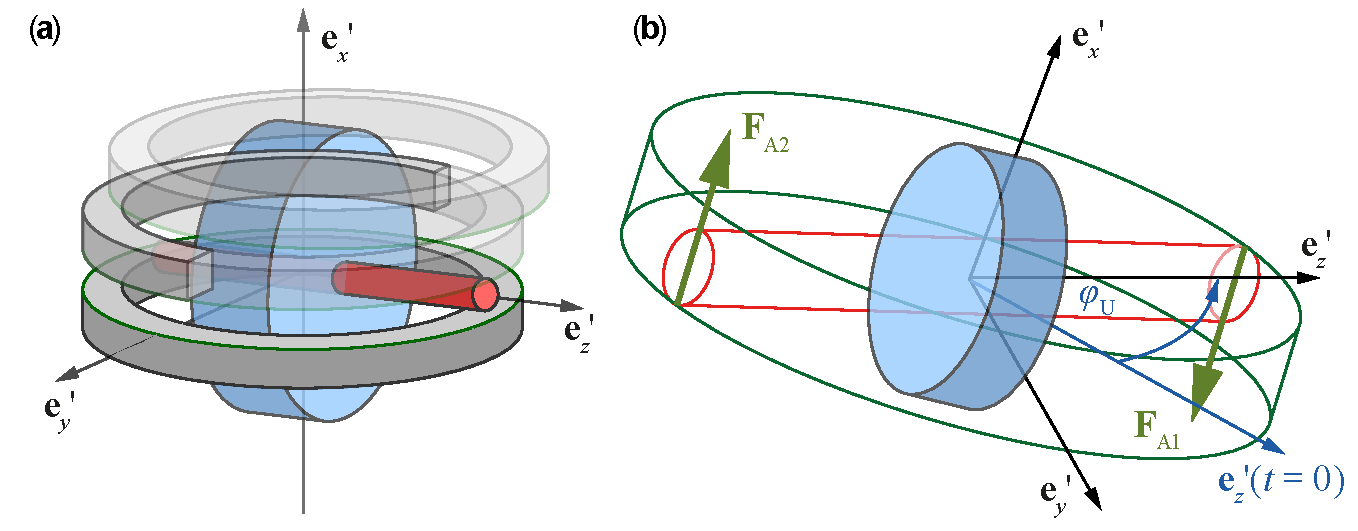
\includegraphics[width=\textwidth]{GyrotwAufbau2.pdf}
  \caption[Geometrie des Kreisels im Gyrotwister.]{Geometrie des Kreisels im
    Gyrotwister: \fa Ein symmetrischer Kreisel wird in einer Nut einer �u�eren
    Halterung gef�hrt. In der Realit�t ist sowohl der Kreisel als auch die
    Halterung nahezu kugelf�rmig.
    \fb Schematische Ausschnittszeichnung mit F�hrungsnut und Achse des Kreisels.
    Achtung: Das eingezeichnete KOS $\tilde{\vec{\Sigma}}'$ bestehend aus den
    Vektoren $\vecpeX$, $\vecpeY$ und $\vecpeZ$ ist nur zum Teil ein
    k�rperfestes System des Kreisels (siehe Text). Zus�tzlich muss beachtet
    werden, dass $\tilde{\vec{\Sigma}}'$ von der Zeit abh�ngt. Will man den
    die Bewegung des Kreisels in der Nut beschreibenden Winkel $\varphi_\text{U}(t)$
    messen, muss man den aktuellen Einheitsvektor $\vecpeZ(t)$ mit
    der Projektion von $\vecpeZ(t=0)$ auf die von $\vecpeX(t)$ und
    $\vecpeZ(t)$ aufgespannte Ebene mit dem Normalenvektor $\vecpeX(t)$ 
    vergleichen. Diese Projektion  $\vecpeZ(t=0)$ ist in der Abbildung blau aufgetragen.}
  \label{abb:bew_GyrotwAufbau2}
\end{figure}

Das Spiel besteht nun darin, durch das
geschickte Bewegen der Hand den Kreisel auf h�here Drehzahlen zu bringen. 
Um zu erkl�ren, wie das funktionieren kann, muss man sich den Aufbau etwas
genauer anschauen. Daf�r greifen wir auf die schematische Zeichnung
in \figref{bew_GyrotwAufbau2} zur�ck. 
%Zun�chst beschreiben, wenn Geh�use fest gehalten.
Dreht man das Geh�use um die $\vecpeX(t)$-Achse,
so wird die Kreisel\-achse aus ihrer urspr�nglichen Rotationsebene gebracht, man �ndert also den
Drehimpuls. Dadurch dr�ckt die Achse auf einer Seite (in der \figref{bew_GyrotwAufbau2}b links)
gegen den unteren Rand der Nut und auf der anderen gegen den oberen Rand.
Diese beiden Kr�fte bewirken das Drehmoment, das n�tig ist, um den Kreisel
zu drehen. Das Ansto�en der Achse an der Nut bewirkt aber noch eine weitere
Bewegung. Der Kreisel rollt (verursacht durch die Rollreibung) an der Nut ab.
Dadurch entsteht eine weitere Drehbewegung.

\begin{figure}
  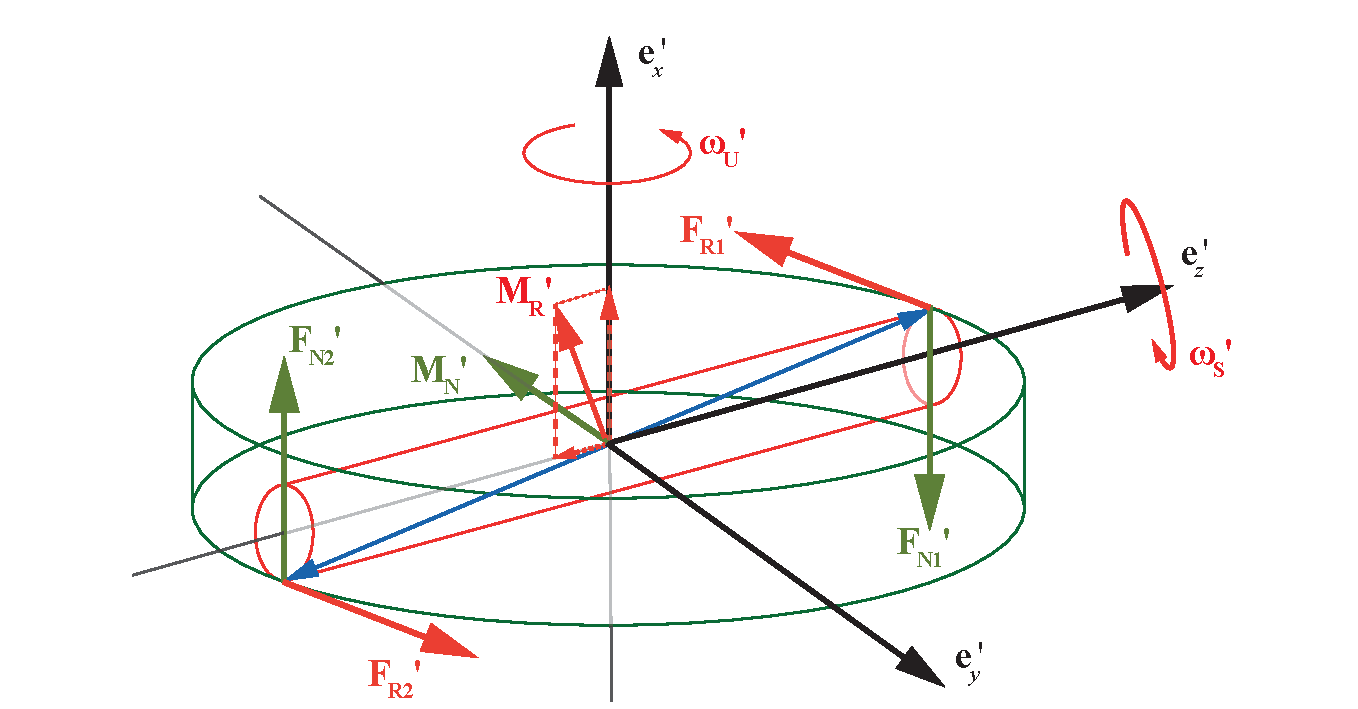
\includegraphics[width=\textwidth]{GyrotwKraefte.pdf}
  \caption[Kr�fte und Drehmomente am Gyrotwister.]{Kr�fte und Drehmomente am
    Gyrotwister bei festgehaltenem Geh�use. Die beiden Auflagekr�fte am
    Nutrand $\vec{F}_{\mathrm{N}1}'$ und $\vec{F}_{\mathrm{N}2}'$ bewirken ein
    Drehmoment, das eine Rotation in der $\vecpeY$-Richtung verhindert. Die
    Reibungskr�fte $\vec{F}_{\mathrm{R}1}'$ und $\vec{F}_{\mathrm{R}2}'$ ergeben
    zusammen mit den zu $\vecpeX$ parallelen Komponenten der Ortsvektoren der
    Auflagepunkte ein Drehmoment  $\vec{M}_\mathrm{R}'$, dessen
    $\vecpeZ$-Komponente eine �nderung von $\omega_S'$ bewirken kann (siehe
    gestrichelt rote Komponenten parallel zur $\vecpeZ$-Achse). Im hier
    gezeigten Fall des nicht bewegten, festgehaltenen Geh�uses zeigt sich
    nur die abbremsende Wirkung der Reibung -- die $z'$-Komponente von
    $\vec{M}_\mathrm{R}'$ wirkt der Drehung entgegen. Das Drehmoment
    $\vec{M}_\mathrm{N}'$, verursacht von den Auflagekr�ften
    $\vec{F}_{\mathrm{N}1}'$ und $\vec{F}_{\mathrm{N}2}'$, kann keine �nderung von
    $\vec{\omega}_\text{s}'$ bewirken, da es senkrecht auf diesem Vektor steht.}.
  \label{abb:bew_GyrotwKraefte}
\end{figure}

Die Bewegung soll mit \figref{bew_GyrotwKraefte} genauer untersucht werden. Dazu folgen wir \cite{Heyda2002}
und w�hlen ein Koordinatensystem $\tilde{\vec{\Sigma}}'$, das sich mit dem Geh�use mitbewegt.
Die $\vecpeX$-Achse steht senkrecht auf der Ebene, in der die Nut liegt. Sie
ist geeignet, um die Drehbewegung des Kreisels aufgrund des Abrollens am
Nutrand zu beschreiben. Die $\vecpeY$-Achse liegt in der Nutebene senkrecht
zur Figurenachse des symmetrischen Kreisels und die $\vecpeZ$-Achse 
entspricht der Figurenachse.
Damit die Lage der $\vecpeY$- und $\vecpeZ$-Achsen zu jeder Zeit so
definiert sein kann, macht das Koordinatensystem die Drehung um die
Figurenachse nicht mit. Das System $\tilde{\vec{\Sigma}}'$ ist also kein vollst�ndig k�rperfestes System des Kreisels.
F�r die Beschreibung der wirkenden Drehmomente und Bewegungen ist es jedoch
hervorragend geeignet. Im gew�hlten Koordinatensystem hat die Bewegung die folgenden Anteile:
\begin{itemize}
\item Die schnelle Rotation des Kreisels erfolgt um die $\vecpeZ$-Achse.
  Sie lautet mit der schnellen Winkelgeschwindigkeit $\omega_\text{S}'$\footnote{Wir kennzeichnen die Vektoren im KOS $\tilde{\vec{\Sigma}}'$ weiterhin als gestrichene Gr��en, die  Winkelgeschwindigkeitskomponenten der Kreiselrotation zur besseren Unterscheidung aber ohne Strich und mit Gro�buchstaben.}
  \begin{equation*}
    \vec{\omega}_\text{S}' = \begin{pmatrix} 0 \\ 0 \\ \Omega_\text{S} \end{pmatrix} \; .
  \end{equation*}
\item Die Rotation durch den Umlauf entlang der Nut entspricht, wie oben
  bereits angemerkt, einer Drehung mit der Umlaufwinkelgeschwindigkeit
  $\omega_\text{U}'$ um die $\vecpeX$-Achse,
  \begin{equation*}
    \vec{\omega}_\text{U}' = \begin{pmatrix} \Omega_\text{U}\\ 0 \\ 0 \end{pmatrix} \; .
  \end{equation*}
\item Zus�tzlich gibt es noch das aktive Eingreifen des Menschen in das
  System durch die Drehbewegung mit der Hand. Wir modellieren diese durch
  eine Drehung um eine raumfeste Achse, die in der Ebene der Nut liegt und deren Lage sich durch die Drehbewegung
  $\vec{\omega}_\text{U}'$ im teilweise k�rperfesten System $\tilde{\vec{\Sigma}}'$ st�ndig �ndert.
  Wir messen die Drehung um die $\vecpeX$-Achse durch den Winkel (\figref{bew_GyrotwAufbau2}b)
  \begin{equation*}
    \varphi_\text{U} = \int_0^t \Omega_\text{U} \,\D t'
  \end{equation*}
  und erhalten damit f�r die Winkelgeschwindigkeit der von der Hand
  verursachten Rotation im KOS
  $\tilde{\Sigma}$
  \begin{equation}
    \vec{\omega}_\text{H}' = \mathbb{R}_{x'}(\varphi_\text{U})\, \vec{\omega}_H
    = \begin{pmatrix} 1 & 0 & 0 \\ 0 & \cos\varphi_\text{U}
      & \sin\varphi_\text{U} \\ 0 & -\sin\varphi_\text{U} & \cos\varphi_\text{U}
    \end{pmatrix} \begin{pmatrix} 0 \\ 0 \\ \Omega_\text{H} \end{pmatrix}
    = \begin{pmatrix} 0 \\ \Omega_\text{H}\,\sin\varphi_\text{U} \\ \Omega_\text{H} \, \cos\varphi_\text{U}
    \end{pmatrix} \; .
    \label{eq:bew_GyrotwRotHand}
  \end{equation}
\end{itemize}
Die gesamte Winkelgeschwindigkeit $\vec{\omega}_\text{ges}'$ des Kreisels lautet damit im KOS $\tilde{\vec\Sigma}'$
\begin{equation*}
  \vec{\omega}_\text{ges}' = \vec{\omega}_\text{S}' + \vec{\omega}_\text{U}' + \vec{\omega}_\text{H}'   =  \begin{pmatrix} \omega_1' \\ \omega_2' \\ \omega_3' \end{pmatrix}
= \begin{pmatrix} \Omega_\text{U} \\ \Omega_\text{H}\,\sin\varphi_\text{U} \\
    \Omega_\text{S} + \Omega_\text{H} \, \cos\varphi_\text{U} \end{pmatrix}
  \; ,
\end{equation*}
wobei $\omega_1'$, $\omega_2'$ und $\omega_3'$ die Komponenten von
$\vec{\omega}_\text{ges}'$ entlang der Achsen $\vecpeX$, $\vecpeY$ und
$\vecpeZ$ darstellen. Hier stellen wir zwei Beziehungen fest. 
\begin{itemize}
	\item Die Rotation durch den Umlauf in der Nut entspricht immer $\omega_1'$. Man kann diese als Pr�zession des symmetrischen Kreisel begreifen. Wir verwenden also im Folgenden die
Identit�ten 
\begin{align}
	\Omega_\text{U} = \omega_1' ~~~ \text{und}  ~~~ \varphi_\text{U} = \varphi_1' = \int_0^t \omega_1' \D t'\,.   \label{eq:bew_Gyrotw_omega1}
\end{align}
\item Zweitens sehen wir, dass $\omega_2'$, also die Rotation um die
  $\vecpeY$-Achse, eindeutig durch die Bewegung der Hand festgelegt ist:
\begin{equation}
  \omega_2' =  \Omega_\text{H}\,\sin\varphi_\text{U}\, \; .
  \label{eq:bew_Gyrotw_omega2}
\end{equation}
Dies ist auch zu erwarten, da die Nut eine freie Rotation um die $\vecpeY$-Achse verhindert.\\
\end{itemize}
F�r die weitere Rechnung und auch den Bezug zu experimentellen Werten ist es sinnvoll, eine geeignete Drehung
$\vec{\omega}_\text{K}'$ im gew�hlten Koordinatensystem $\tilde{\vec{\Sigma}}'$ zu definieren, mit der sich $\vec{\omega}_\text{S}'$  gegen�ber dem raumfesten
System relativ bewegt. Diese Drehung $\vec{\omega}_\text{K}'$ enth�lt nur die Anteile $\vec{\omega}_\text{U}' = \vec{\omega}_1'$ und
$\vec{\omega}_\text{H}'$, nicht jedoch die schnelle Drehung $\vec{\omega}_\text{S}'$ um die
Figurenachse\footnote{Wie oben erw�hnt, haben wir kein echtes k�rperfestes
  Koordinatensystem verwendet. Damit bleibt der Vektor $\vecpey$ immer in der
  Nutebene liegen und die weitere Rechnung �bersichtlich.},
\begin{equation*}
  \vec{\omega}_\text{K}' = \vec{\omega}_\text{ges}' - \vec{\omega}_\text{S}' =
  \begin{pmatrix} \omega_1' \\ \Omega_\text{H}\,\sin\varphi_1' \\
    \Omega_\text{H}\,\cos\varphi_1' \end{pmatrix} \; .
\end{equation*}

Mit den Tr�gheitsmomenten $J_{12}$ f�r Rotationen senkrecht zur Figurenachse
und $J_3$ f�r Rotationen um die Figurenachse lautet der Drehimpuls im teilweise mitbewegten System $\tilde{\vec{\Sigma}}'$:
\begin{equation*}
  \vec{L}' = \begin{pmatrix} J_{12}\: \omega_1' \\ J_{12}\: \omega_2' \\ J_3\: \omega_3' \end{pmatrix} \,.
\end{equation*}

Die Kreiselgleichungen ergeben sich im raumfesten Koordinatensystem aus dem 
\KOS{} $\tilde{\vec{\Sigma}}'$, das mit $\vec{\omega}_\text{K}'$ rotiert,
zu (\vgl \eqref{eq:bew_Rot_System5})
\begin{equation*}
  \frac{\D}{\D t} \vec{L} = \frac{\D}{\D t} \vec{L}' + \vec{\omega}_\text{K}' \times
  \vec{L}' = \MD' \,.
\end{equation*}
Die Ableitung des Drehimpulses im \KOS{} $\tilde{\vec{\Sigma}}$ l�sst sich in Komponenten aufschreiben zu
\begin{align}
  \frac{\D}{\D t} \vec{L}' + \vec{\omega}_\text{K}' \times \vec{L}'
  &= \begin{pmatrix} J_{12}\: \dot{\omega}_1' \\ J_{12}\:
    \dot{\omega}_2' \\ J_3\: \dot{\omega}_3' \end{pmatrix}
  + \begin{pmatrix} \omega_1' \\ \Omega_\text{H}\,\sin\varphi_1' \\
    \Omega_\text{H} \,\cos\varphi_1'\end{pmatrix} \times \begin{pmatrix} J_{12}\:
    \omega_1' \\ J_{12}\: \omega_2' \\ J_3\: \omega_3' \end{pmatrix} \notag \\
  &= \begin{pmatrix}
    J_{12}\:\dot{\omega}_1' + J_3 \:\Omega_\text{H}\,\omega_3'\,\sin\varphi_1'
    - J_{12}\: \Omega_\text{H}\,\omega_2'\,\cos\varphi_1' \\
    J_{12}\:\dot{\omega}_2' + J_{12} \:\Omega_\text{H}\,\omega_1'\,\cos\varphi_1'
    - J_3\: \omega_1'\,\omega_3' \\
    J_3\:\dot{\omega}_3' + J_{12}\: \left (\omega_1'\, \omega_2' - 
      \Omega_\text{H} \,\omega_1' \,\sin\varphi_1'\,\right )
  \end{pmatrix} = \MD'\; .
  \label{eq:bew_Gyrotw_drehimp}
\end{align}
Wir m�ssen jetzt noch das Drehmoment $\MD'$ berechnen, damit wir die Bewegungsgleichung nach den einzelnen $\omega_i(t)'$ l�sen k�nnen. Man kann das Drehmoment in zwei Beitr�ge aufteilen:
\begin{itemize}
\item Die Auflagekr�fte auf der Nut $\vec{F}_{\text{N},i}'$, die verhindern,
  dass eine Rotation um die $\vecpeY$-Achse stattfinden kann, bewirken ein
  Drehmoment $\vec{M}_\text{N}'$.
  Dieses liegt senkrecht zum Ortsvektor der Auflagepunkte (blau in
  \figref{bew_GyrotwKraefte}) und senkrecht zur $\vecpeX$-Achse\footnote{Die
    Kr�fte vom Nutrand auf die Achse sind parallel zu $\vecpeX$ gerichtet.}.
  Es zeigt im Beispiel aus \figref{bew_GyrotwKraefte} in Richtung der
  negativen $\vecpeY$-Achse.
  \begin{equation}
    \vec{M}_\text{N}' = r\,\vecpeZ \times F \,\vecpeX = M_0\, \vecpeY
    \label{eq:bew_GyrotwNutDrehmoment}
  \end{equation}
  Der Betrag $M_0$ dieses Drehmoments muss uns nicht bekannt sein. Vielmehr
  k�nnen wir es sp�ter aus der Bedingung, dass $\omega_2'$ fest durch $\Omega_\text{H}$ gegeben ist,
  berechnen.

  Wir sehen hier �brigens auch eines der Charakteristika des Gyrotwisters.
  Das von den Auflagekr�ften verursachte Drehmoment
  ist ausschlie�lich parallel zu $\vecpeY$ gerichtet und kann somit wie oben erw�hnt auf keinen
  Fall zu einer Beschleunigung der schnellen Drehbewegung $\vec{\omega}_s'$
  beitragen.\footnote{Selbst wenn man ganz korrekt betrachtet, dass der Vektor
    vom Mittelpunkt des Kreisels zu den Auflagepunkten nicht rein in
    $\vecpeZ$-Richtung zeigt, sondern eine $\vecpeX$ Komponente haben muss,
    tr�gt dies nichts zum Drehmoment bei, da der zur Kraft parallele Anteil des
    Ortsvektors kein Drehmoment verursacht, wie man auch leicht am Kreuzprodukt
    erkennen kann.}

\item Die durch die Bewegung der Hand vermittelte Drehung $\vec{\omega}_\text{H}'$ bewirkt ein weiteres Drehmoment $\vec{M}_\text{H}'$, denn sie �ndert
  offensichtlich nach \eqref{eq:bew_Gyrotw_drehimp} alle Drehimpulskomponenten.
  Diesen Teil extrahieren wir und betrachten die �nderungsrate
  $\D \vec{L}'/\D t$, die dieses Drehmoment aufbringen muss,
  \begin{equation}
    \vec{M}_\text{H}' = \vec{\omega}_\text{H}' \times J_{12}\, \vec{\omega}_\text{U}' = \begin{pmatrix}
      0 \\ \Omega_\text{H} \,\sin\varphi_1'\\ \Omega_\text{H}\,\cos\varphi_1' \end{pmatrix}
    \times \begin{pmatrix} J_{12}\:\omega_1' \\ 0 \\ 0 \end{pmatrix}
    =  \begin{pmatrix} 0 \\ J_{12}\: \Omega_\text{H} \,\omega_1' \,\cos\varphi_1' \\
      - J_{12}\: \Omega_\text{H} \,\omega_1'\,\sin\varphi_1' \end{pmatrix} \;.
    \label{eq:bew_GyrotwDefMH}
  \end{equation}
\end{itemize}

Das gesamte Drehmoment $\MD'$ lautet somit
\begin{equation}
  \MD' = \vec{M}_\text{N}' + \vec{M}_\text{H}'
  =  \begin{pmatrix} 0 \\ M_0 + J_{12}\, \Omega_\text{H} \,\omega_1'\,\cos\varphi_1'
    \\ - J_{12}\,\Omega_\text{H} \,\omega_1'\, \sin\varphi_1' \end{pmatrix} \; .\label{eq:bew_GyrotwTotalMD}
\end{equation}
Dies fasst man mit \eqref{eq:bew_Gyrotw_drehimp} zu den
Bewegungsgleichungen f�r die Komponenten der Winkelgeschwindigkeit $\vec{\omega}_\text{ges}'$ zusammen,
\begin{subequations}
  \begin{align}
    J_{12}\, \dot{\omega}_1' &= - J_3\,\Omega_\text{H} \,\omega_3' \,\sin\varphi_1'+
                               J_{12}\, \Omega_\text{H}\, \omega_2' \,\cos\varphi_1'\; ,\\
    J_{12}\, \dot{\omega}_2' &= J_3\, \omega_1' \,\omega_3' + M_0 \; ,
    \label{eq:bew_GyrotwDGLomega2}\\
    J_3\, \dot{\omega}_3' &= - J_{12}\, \omega_1' \,\omega_2' \; .
  \end{align}
\end{subequations}

Wir interessieren uns vor allem f�r die �nderung von $\vec{\omega}_\text{S}'$. Nun wissen wir au�erdem, dass
$\omega_2'$ nach \eqref{eq:bew_Gyrotw_omega2} abh�ngig von anderen Gr��en, \ua  von der Bewegung der Hand ($\Omega_\text{H}$) ist. Benutzen wir die Beziehung \eqref{eq:bew_Gyrotw_omega2}, die $\omega_2'$ mit $\Omega_\text{H}$ koppelt, erhalten
wir die beiden gekoppelten Bewegungsgleichungen f�r $\dot{\omega}_1'$ und  $\dot{\omega}_3'$:
\begin{subequations}
  \begin{align}
    J_{12}\, \dot{\omega}_1' &= - J_3\,\Omega_\text{H} \,\omega_3'\,\sin\varphi_1' +
                               J_{12}\, \Omega_\text{H}^2\,\cos\varphi_1'\,\sin\varphi_1'\; , \label{eq:bew_GyrotwDGLomega1} \\
    J_3\, \dot{\omega}_3' &= - J_{12}\,\Omega_\text{H}\,\omega_1' \,\sin\varphi_1'\; . \label{eq:bew_GyrotwDGLomega3}
  \end{align}
\end{subequations}
Man sieht aus Gl. \eqref{eq:bew_GyrotwDGLomega3}, dass sich die Geschwindigkeit $\omega_3'$ der schnellen Rotation um die $\vecpeZ$-Achse also tats�chlich �ndern kann.
Allerdings besagt Gleichung \eqref{eq:bew_GyrotwDGLomega3} vorerst nur, dass
eine �nderung von $\omega_3'$ m�glich ist. Wie erreichen wir aber gezielt eine
Beschleunigung, \dh ein Anwachsen von $\omega_3'$? Dazu m�ssen wir
sicherstellen, dass $\dot{\omega}_3'$ durchg�ngig dasselbe Vorzeichen hat wie
$\omega_3'$. Gehen wir davon aus, dass zu einem Zeitpunkt am Anfang der
Bewegung $\omega_3' > 0$ und $\omega_1' > 0$ sind (\figref{bew_GyrotwKraefte}),
dann ist die Bedingung f�r eine Beschleunigung ganz sicher erf�llt, wenn
\begin{equation}
  \Omega_\text{H}(t) = - \hat{\Omega}_\text{H}\, \sin \varphi_1'(t)
  \label{eq:bew_Gyrotw_omegaH}
\end{equation}
gilt, worin $\hat{\Omega}_\text{H}$ die Amplitude der Handbewegung und positiv
ist. Dann werden die Bewegungsgleichungen \eqref{eq:bew_GyrotwDGLomega1} und
\eqref{eq:bew_GyrotwDGLomega3} zu
\begin{align}
  J_{12}\, \dot{\omega}_1' &= J_3\,\hat{\Omega}_\text{H} \,\omega_3'\,\sin^2\varphi_1'\,  +\,
                             J_{12}\,\hat{\Omega}_\text{H}^2\,\cos\varphi_1'\,\sin^3\varphi_1'\; , \\
  J_3\, \dot{\omega}_3' &= J_{12}\,\hat{\Omega}_\text{H}\,\omega_1' \sin^2\varphi_1'\;. \label{eq:bew_GyrotwDGLoptomega3}
\end{align}
Das Geheimnis des Gyrotwisters besteht also darin, die Hand immer mit der Frequenz der Rotation
$\omega_1'(t)$ zu bewegen.\footnote{Man  erkennt an \eqref{eq:bew_GyrotwDGLoptomega3} auch sofort, dass bei nicht bewegter Hand ($\hat{\Omega}_\text{H}=0$ sofort $\omega_1 = \mathrm{const}$ (Pr�zession) und $\omega_3 = \mathrm{const}$ (schnelle Kreiselrotation) folgt. Die abbremsenden Reibungskr�fte sind hier nicht modelliert.} Dabei ist die Phasenlage wichtig. Der Winkel $\varphi_1' =
\varphi_\text{U}'$ beschreibt den Umlauf des Kreisels in der Nut. Die Komponente
von $\vec{\omega}_\text{H}'$ entlang der Figurenachse $\vecpeZ$ lautet nach
\eqref{eq:bew_GyrotwRotHand} gerade $\Omega_\text{H}\cos\varphi_\text{U}$.
Die Geschwindigkeit von $\Omega_\text{H}$ ist nach \eqref{eq:bew_Gyrotw_omegaH}
proportional zu $-\sin \varphi_U$. Sie muss der Figurenachse also um
$\pi/2$ vorauseilen.

\begin{figure}
  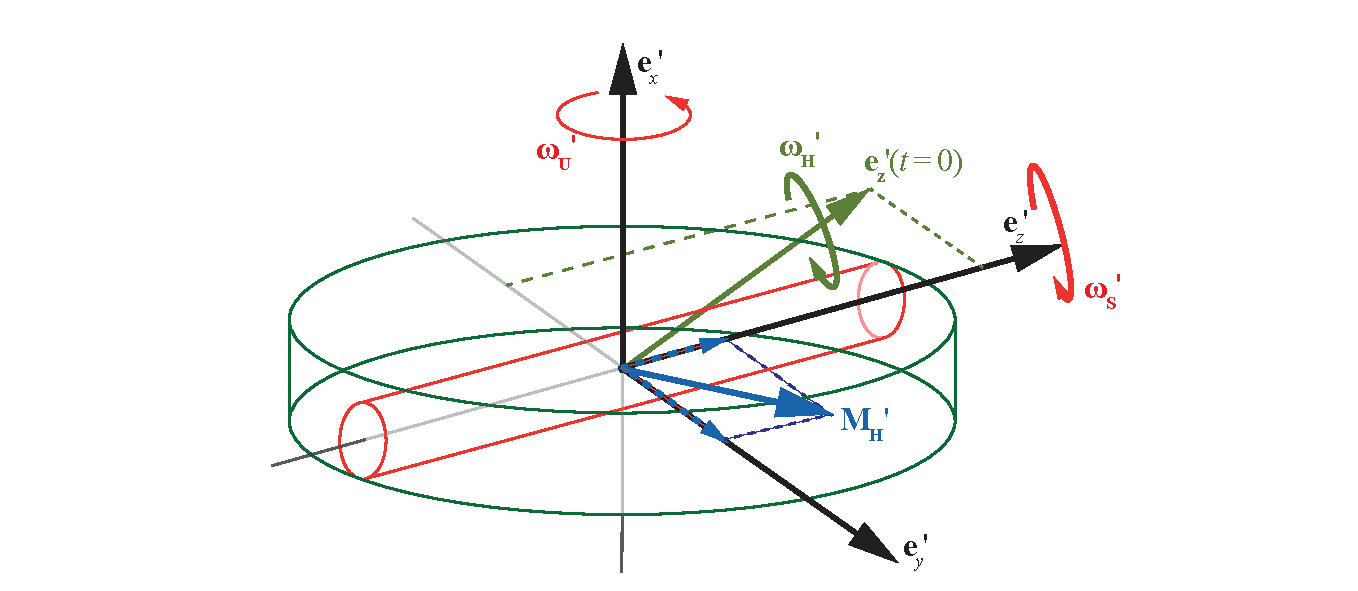
\includegraphics[width=\textwidth]{GyrotwHand.pdf}
  \caption[Bewegung der Hand am Gyrotwister.]{Bewegung der Hand am
    Gyrotwister. Durch die Drehung des Geh�uses entgegen der Drehrichtung
    des Kreisels bewirkt man das Drehmoment $\vec{M}_\text{H}$, das die
    Rotation um die $\vecpeZ$-Achse beschleunigt.}
  \label{abb:bew_GyrotwHand}
\end{figure}

Um physikalisch zu verstehen, warum das gerade zu einer Beschleunigung
f�hrt, betrachten wir noch einmal die wirkenden Kr�fte und Drehmomente.
\figref{bew_GyrotwKraefte} zeigt die Ortsvektoren vom Mittelpunkt
des Kreisels zu einem der Auflagepunkte (blau) sowie die Auflagekr�fte (gr�n)
und die Reibungskr�fte (rot) mit den jeweils sich dazu ergebenden Drehmomenten.
Man erkennt, dass die zu $\vecpeX$ parallele Komponente des Ortsvektors zum
Auflagepunkt zusammen mit den Reibungskr�ften $\vec{F}_{\text{R}1}'$ und
$\vec{F}_{\text{R}2}'$ einen Beitrag zum Drehmoment parallel zu $\veceZ$
leisten kann. Wir erkennen jetzt auch, warum wir ein Lager mit Spiel brauchen.
Die Achse des Kreisels muss sich in der Nut leicht verdrehen k�nnen, sodass
sie nur an einer Seite anst��t. Nur so kann die Abrollbewegung $\omega_1'$
in Gang kommen, die essentiell ist, und eine Beschleunigung der schnellen
Drehung des Kreisels $\omega_3'$ zu bewirken, vgl.
\eqref{eq:bew_GyrotwDGLomega3}. Die oben beschriebene Bewegung des Geh�uses
sorgt nun �ber zus�tzliche Kr�fte durch die Hand daf�r, dass der Kreisel
von der Bewegung des Geh�uses mitgenommen wird und sich das Abrollen
beschleunigt. Dazu schauen wir uns \figref{bew_GyrotwHand} an. Die
Rotationsbewegung der Hand erfolgt nach \eqref{eq:bew_GyrotwRotHand} um
die $\vecpeZ(t=0)$-Achse (gr�ne Achse in der Abbildung), das Drehmoment
ergibt sich dann nach \eqref{eq:bew_GyrotwDefMH} um $\pi/2$ phasenversetzt
(blau). Die Komponente entlang der momentanen $\vecpeZ$-Achse sorgt
f�r die Beschleunigung der Rotation des Kreisels.

Nun wollen wir noch ermitteln, wie gro� der Betrag des von der Nut ausge�bten Drehmoments $\left|\vec{M}_\text{N}'\right| =  M_0$ ist.
Dieser ergibt sich aus der Bedingung, dass Gleichung \eqref{eq:bew_GyrotwDGLomega2}
f�r das $\omega_2'$ aus der Zwangsbedingung \eqref{eq:bew_Gyrotw_omega2}
erf�llt sein muss. Weiterhin wollen wir den Fall \eqref{eq:bew_Gyrotw_omegaH}
betrachten, in dem die maximale Energie eingekoppelt wird. Fasst man alles
zusammen, erh�lt man
\begin{align}
  M_0 &= J_{12}\: \dot{\omega}_2' - J_3\, \omega_1'\, \omega_3' ~~\text{\bzw} \nonumber \\
  M_0 &= -2 J_{12}\: \hat{\Omega}_\text{H}\,\omega_1'\, \cos\varphi_1' \, \sin\varphi_1' \, 
	       - J_3\: \omega_1'\,\omega_3' \;.    \label{eq:bew_gyrotwo_M0}
\end{align}
Es soll betont werden, dass wir in der gesamten Betrachtung die beiden
Winkelgeschwindigkeiten $\omega_1'$  und $\omega_3'$ als unabh�ngig betrachtet
haben. Das widerspricht der Anmerkung vom Anfang, dass die Drehung
$\omega_1'$ durch das Abrollen am Nutrand zustande kommt. Daf�r muss die
Rollbedingung
\begin{equation*}
  \omega_1 = \frac{R_\text{N}}{R_\text{A}}\omega_3
\end{equation*}
durchg�ngig erf�llt sein, wobei $R_\text{N}/R_\text{A}$ das Verh�ltnis des Nutradius zum Achsenradius des Kreisels beschreibt. Die Rollbedingung l�sst 
damit nur eine unabh�ngige Variable zu. Tats�chlich ist das Rollen aber auch nicht
immer erf�llt. Bei h�heren Geschwindigkeiten f�ngt die Achse meist an, am
Nutrand entlang zu rutschen, sodass tats�chlich wieder zwei unabh�ngige
Variablen vorliegen. Liegt ein reines Abrollen vor, muss die zus�tzliche
Zwangsbedingung selbstverst�ndlich ber�cksichtigt werden. Weiterhin haben
wir vernachl�ssigt, dass durch die leichte Schr�glage in der Nut der
Basisvektor $\vecpeX$ streng genommen nicht senkrecht auf der Nutebene steht
und die  Vektoren $\vecpeY$ und $\vecpeZ$ nicht exakt in der Nutebene liegen.
Das hat zur Folge, dass $\vec{\omega}_\text{H}'$ eine (wenn auch sehr kleine)
Komponente in $\vecpeX$-Richtung besitzt. Das ver�ndert die Ergebnisse
jedoch nur geringf�gig \cite{Heyda2002}. Eine Analyse, die dies ber�cksichtigt,
findet sich in \cite{Gulick2000}.

In der numerischen L�sung, die mit dem 
\mscr{} \mlbewref{Gyrotwister.m} erzeugt wurde, sehen wir, dass sich $\omega_3'$ tats�chlich
mit einer positiven Steigung �ndert.
Dies ist in Abbildung \figref{bew_Gyrotwomega3} dargestellt.

\begin{figure}
  \centering
  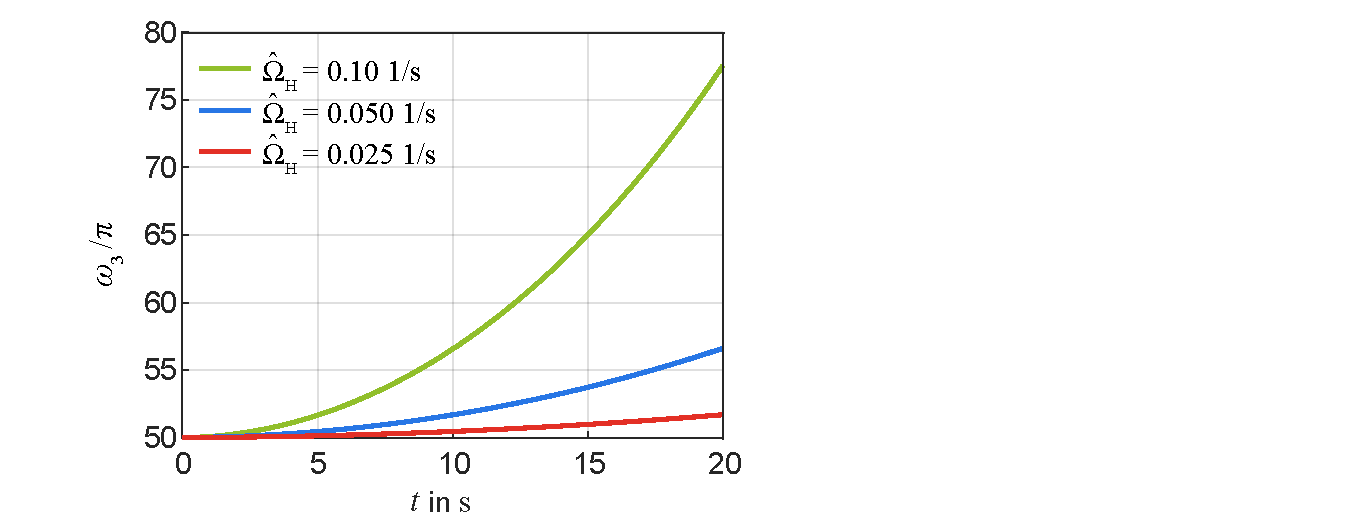
\includegraphics[width=\textwidth]{Gyrotwister1.pdf}
  \caption[Beschleunigung des Kreisels im Gyrotwister.]{Beschleunigung des
    Kreisels im Gyrotwister durch die Bewegung mit der Hand. Hier wird die
    optimale Einkopplung an Energie nach Gleichung \eqref{eq:bew_Gyrotw_omegaH}
    angenommen. Die Frequenz $\omega_3'$ steigt offensichtlich mit der Zeit an. Parameter siehe \mscr{} \mlbewref{Gyrotwister.m} }
  \label{abb:bew_Gyrotwomega3}
\end{figure}

Man kann auch gut erkennen, dass eine Phasendifferenz entscheidend f�r die
Beschleunigung ist.
Die Berechnungen dazu sind im \mscr{} \mlbewref{GyrotwisterPhase.m} zu finden.
In Abbildung \figref{bew_GyrotwPD} (links) ist der damit ermittelte Zeitverlauf von
$\omega_3'$ f�r verschiedene Phasendifferenzen $\Delta\phi$ zum optimalen Fall
\begin{equation}
  \Omega_\text{H} = - \hat{\Omega}_\text{H}\, \sin \left ( \varphi_1' +\Delta \phi \right )
  \label{eq:bew_Gyrotw_omegaHdiff}
\end{equation}
aufgetragen.
F�r $\Delta\phi = 0.2\pi$ ist der Anstieg von $\omega_3'$ erkennbar reduziert.
Bewegt man die Hand um $\Delta\phi=\pi/2$ phasenverschoben
zum optimalen Fall (also um $\pi/2$ Phasenverschoben zur Bewegung von
$\omega_1'$), so koppelt man im Mittel keine Energie ein.
Die Frequenz $\omega_3'$ �ndert sich gar nicht.
Das tut sie jedoch wieder f�r eine
Phasenverschiebung von $\Delta\phi=\pi$.
Auf den ersten Blick mag das �berraschen.
Intuitiv w�rde man einen negativen Effekt erwarten.
Schaut man sich die Bewegung von $\omega_1'$ an, erkennt man auch, dass genau das der
Fall ist (Abbildung \figref{bew_GyrotwPD} rechts).
Die Rotation $\omega_1'$
kehrt sich in diesem Fall um und wird in die entgegengesetzt Richtung beschleunigt.
Dann ist man zwar immer noch mit $\omega_1'$ synchron, aber
es tritt jetzt die ben�tigte Phasenverschiebung zu $\omega_3'$ auf, um wieder
eine Beschleunigung erzielen zu k�nnen.
In Gleichung
\eqref{eq:bew_GyrotwDGLoptomega3} heben sich das Minuszeichen durch die
Phasenverschiebung um $\pi$ aus Gleichung \eqref{eq:bew_Gyrotw_omegaHdiff}
und das Minuszeichen von $\omega_1'$ gegenseitig auf.

\begin{figure}
  \centering
  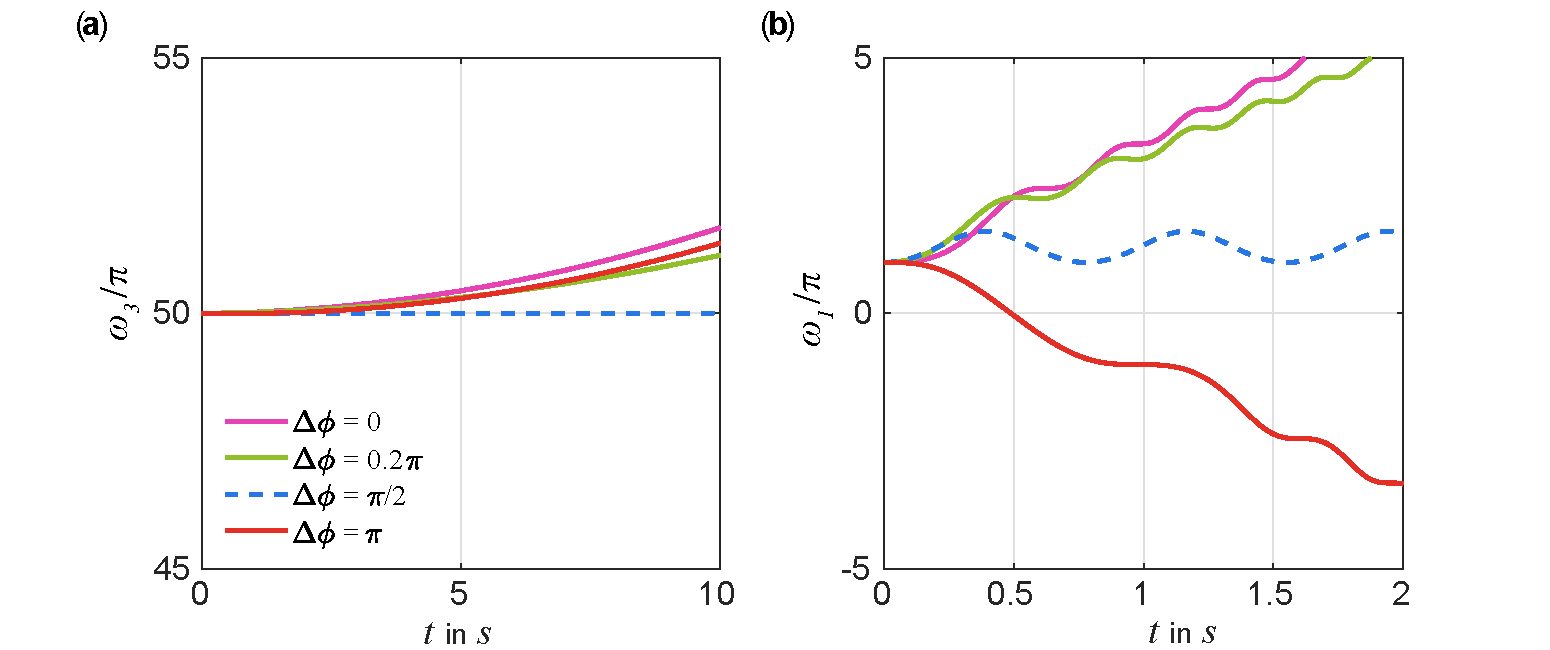
\includegraphics[width=\textwidth]{Gyrotwister2.pdf}
  \caption[Beschleunigung des Kreisels im Gyrotwister mit Phasendifferenz.]
  {\fa Beschleunigung des Kreisels im Gyrotwister mit einer Phasendifferenz
    $\Delta\phi$ zum optimalen Fall nach \eqref{eq:bew_Gyrotw_omegaHdiff}
    und zugeh�rige \fb Entwicklung von $\omega_1'$ (rechts). Nur f�r
    den optimalen Fall $\Delta\phi=0$ erzielt man die maximale Beschleunigung
    von $\omega_3'$. F�r andere Phasenbeziehungen ist sie abgeschw�cht, im
    Fall $\Delta\phi=\pi/2$ verschwindet sie sogar vollst�ndig. F�r
    $\Delta\phi=\pi$ sorgt die Umkehrung der Rotationsrichtung von
    $\omega_1'$ daf�r, dass wieder eine Beschleunigung eintritt.}
  \label{abb:bew_GyrotwPD}
\end{figure}

M�chte man nur grobe qualitative Ergebnisse erhalten, kann man davon
ausgehen, dass $\Omega_\text{H}(t)$ sich im Vergleich mit der schnellen Rotation
des Kreisels nur langsam ver�ndert \cite{Heyda2002}, was eine vern�nftige
Annahme ist. Dann kann man auch mittlere
Frequenzen $\bar{\omega}_1'$ und $\bar{\omega}_3'$ einf�hren und es gilt $\varphi_1' = \bar{\omega}_1'
\,t$. Die Absch�tzungen f�r die Beschleunigung der
Kreiselrotation lauten damit:
\begin{align*}
  \frac{\Delta \bar{\omega}_3'}{\Delta t} &= \lk \frac{1}{2\pi} \int_0^{2\pi} \sin^2\varphi_1'\,\D\varphi_1' \rk \, \frac{J_{12}}{J_3 } \, \hat{\Omega}_\text{H} \, \bar{\omega}_1' 
                                           = \frac{1}{2} \frac{J_{12}}{J_3 } \,\hat{\Omega}_\text{H} \,\bar{\omega}_1'\\
  \intertext{bzw. f�r das Drehmoment $\bar{M}_0 $}
  \bar{M}_0 &= - J_3 \:\bar{\omega}_1'\, \bar{\omega}_3' \; .
\end{align*}

In \probref{bew_gyrotwister} wollen wir den Gyrotwister als Trainingsger�t betrachten und die Kr�fte und die Muskelarbeit berechnen, die man bei einem Gyrotwister aufbringen muss, und dies zu einem vergleichbaren Training mit Heben einer Hantel mit einer Masse von $\SI{3}{\kg}$ in Beziehung setzen.


\newpage
\subsection{Der Kreiselkompass, ein nordsuchender Kreisel} \index{Kreisel!nordsuchender}\index{Kreiselkompass} \label{kap:bew_gyro}

\textbf{Zur Geschichte des Kreiselkompasses}\\

Unter einem klassischen Gyroskop\index{Gyroskop} (Kreiselinstrument) versteht man einen schnell rotierenden, symmetrischen Kreisel, der sich in einem beweglichen Lager, \zb einer kardanische Aufh�ngung\index{Aufh�ngung!kardanische} befindet. 
Das erste Gyroskop wurde 1810 von J.G.F.~Bohnenberger\footnote{Johann Gottlieb Friedrich Bohnenberger (1765--1831) war ein deutscher Astronom, Mathematiker, Mechaniker und Physiker, der auch als Geod�t wichtige Beitr�ge erbrachte. Er gilt als Begr�nder der Landesvermessung W�rttembergs.}\indexp{Bohnenberger, Johann Gottlieb Friedrich} an der Universit�t T�bingen erfunden \cite{Wagner2005} und 1852 von L.~Foucault\indexp{Foucault, Jean Bernard L�on} weiterentwickelt (\figref{bew_GyroBohnenberger}b). Diese Ger�te bilden den Ursprung aller sp�teren Kreiselger�te
%f�r die beiden Anwendungsgebiete Navigation und Stabilisierung. Dies betrifft die 
wie Kreiselkompasse, k�nstliche Horizonte und Wendezeiger f�r die Navigation oder auch Kreiselstabilisatoren f�r die Schiff- und Raumfahrt. Selbst die heute in vielen Smartphones und Drohnen eingebauten Inertialplattformen gehen letztendlich auf das Gyroskop-Prinzip zur�ck \cite{Wagner2023}.\\
Interessanterweise war das Gyroskop zun�chst ein Ger�t der physikalischen Grundlagenforschung und Lehre. Es dauerte fast 100 Jahre bis zum Anfang des 20. Jahrhunderts, bis die ersten technischen Anwendungen in der Navigation m�glich wurden (\probref{bew_gyroskope}). 

\begin{figure}
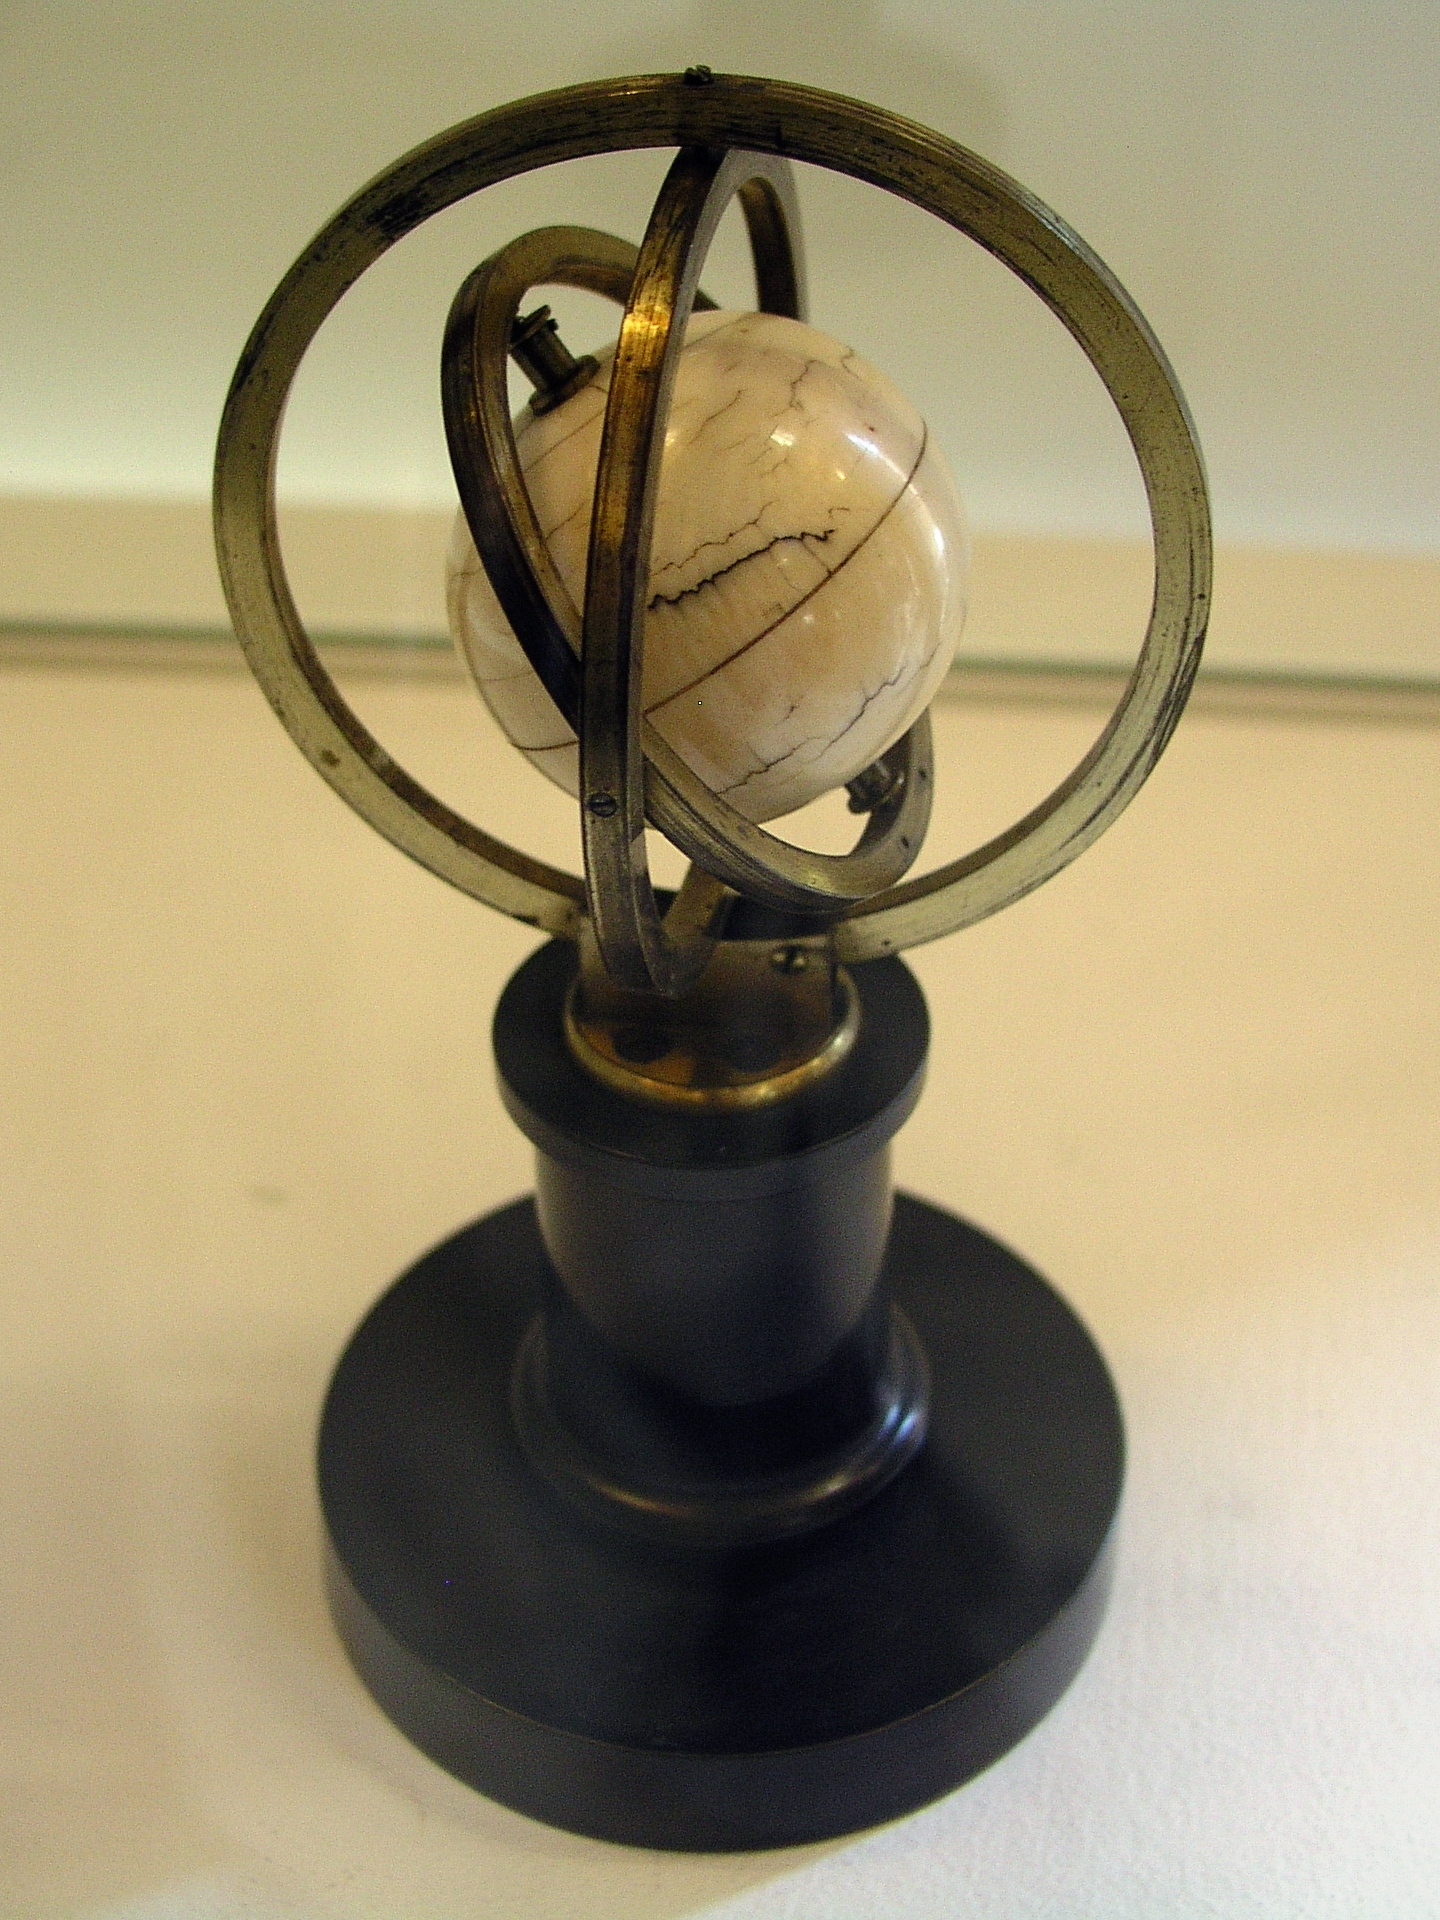
\includegraphics[width=\textwidth]{GyroBohnenberger.pdf}
\caption[Original-Gyroskop von Bohnenberger und Kugelkreiselkompass.]{\fa Das Original-Gyroskop von J.G.F.~Bohnenberger. Ein Exemplar steht im T�binger Stadtmuseum. \fb Foucault's Variante des Gyroskops von Bohnenberger. Freundliche �berlassung von J.F Wagner \cite{Wagner2005, Wagner2023}. \fc Kugelkreiselkompass der Firma Ansch�tz.} %\bzw Wikimedia Commons.
\label{abb:bew_GyroBohnenberger}
\end{figure}

Die Nutzung eines Kreisels f�r die Navigation in der Schifffahrt
hatte zu Beginn des 20.~Jahrhunderts enorme
Bedeutung gewonnen, insbesondere weil ein magnetischer Kompass in der N�he der
Pole zu ungenau ist und in U-Booten mit ihrer Metallh�lle �berhaupt nicht funktioniert.
Hermann Ansch�tz-Kaempfe\indexp{Ansch�tz-Kaempfe, Hermann}%
\footnote{Hermann Ansch�tz-Kaempfe (1872--1931) war ein deutscher Wissenschaftler, der 1905 in Kiel das Unternehmen Ansch�tz \& Co gr�ndete, welches er bis 1930 leitete und dann an die Carl-Zeiss-Stiftung �bertrug. 
%Heute geh�rt das Unternehmen zur Raytheon Gruppe. 
Ansch�tz-Kaempfe entwickelte zusammen mit seinem Vetter Max Schuler den ersten bordtauglichen Kreiselkompass, der 1907 vorgestellt wurde. Ab 1919 wurde daraus der nach Ansch�tz-Kaempfe benannte \anf{Ansch�tz-Zweikreisel-Kugelkompass}.
Dieser Kompass diente als Grundlage moderner Kreiselkompass-Systeme.}
baute als erster auf Basis eines Kreisels einen verl�sslichen Kompass\cite{Lohmeier1992}, der sich selbstt�tig nach Norden ausrichtet.\footnote{Ein Patent f�r die Entwicklung von Ansch�tz-Kaempfe wurde 1904
  angenommen. In einem Patentstreit mit einem amerikanischen Erfinder eines 
  Konkurrenzproduktes wurde Albert Einstein\indexp{Einstein, Albert} als Gutachter hinzugezogen. Aus den Gespr�chen ist
  ein enger Kontakt zwischen Hermann Ansch�tz-Kaempfe und Albert Einstein entstanden, der zu
  zahlreichen Diskussionen �ber die technische Verbesserung des Kreiselkompasses f�hrte
  \cite{Lohmeier1992}.}\\ 
Diese elektromechanischen Kreiselkompasse waren zu ihrer Zeit und sind es auch heute noch wahre Wunderwerke der Mechanik. Ihre Kreiselachsen sind h�ufig f�r die notwendige horizontale Fixierung in komplexen Konstruktionen oder Fl�ssigkeiten gelagert und werden mit elektrischen Motoren mit Drehzahlen bis zu $\SI{75000}{\per\minute}$ angetrieben. Die Orientierungsgenauigkeit ist besser als 10 Winkelsekunden pro Tag, wobei die Einstellzeit des Kreisels auf Nord durchaus einige Stunden betragen kann. \cite{BergmannSchaefer1998}\\

\textbf{Physikalisches Prinzip des klassischen Kreiselkompasses}\\

Um zu verstehen, warum sich ein solcher Kreisel �berhaupt nach Norden
ausrichtet, muss man ber�cksichtigen, dass sich der Kreisel in einem
Nichtinertialsystem befindet. Bisher hatten wir alle Kreisel
nur in einem Inertialsystem betrachtet.
Wir wollen zun�chst eine qualitative physikalische Beschreibung der
Funktionsweise eines Kreiselkompass auf Basis der Newtonschen Mechanik geben
und anschlie�end eine quantitative Rechnung im Lagrange-Formalismus zeigen.\\

Wir betrachten zun�chst das Verhalten eines sogenannten frei drehbaren Kreisels\index{Kreisel!freier}\index{Gyroskop!freies} nach \figref{bew_GyroBohnenberger}a und \figref{bew_GyroCompassExpl01}a. Dessen Drehimpuls bleibt relativ zum Inertialsystem unver�ndert im Raum orientiert, da auf ihn wegen der entsprechenden Lagerung kein Drehmoment wirkt. Wenn er auf einen Stern ausgerichtet war, dann bleibt er auch unabh�ngig von seiner Mitbewegung auf der Erdoberfl�che auf diesen Stern ausgerichtet. F�r einen mitbewegten Erdbeobachter erscheint es daher so, als w�rde ein Ende der Kreiselachse im Laufe eines Tages im Osten aufgehen und im Westen untergehen.\\
\begin{figure}
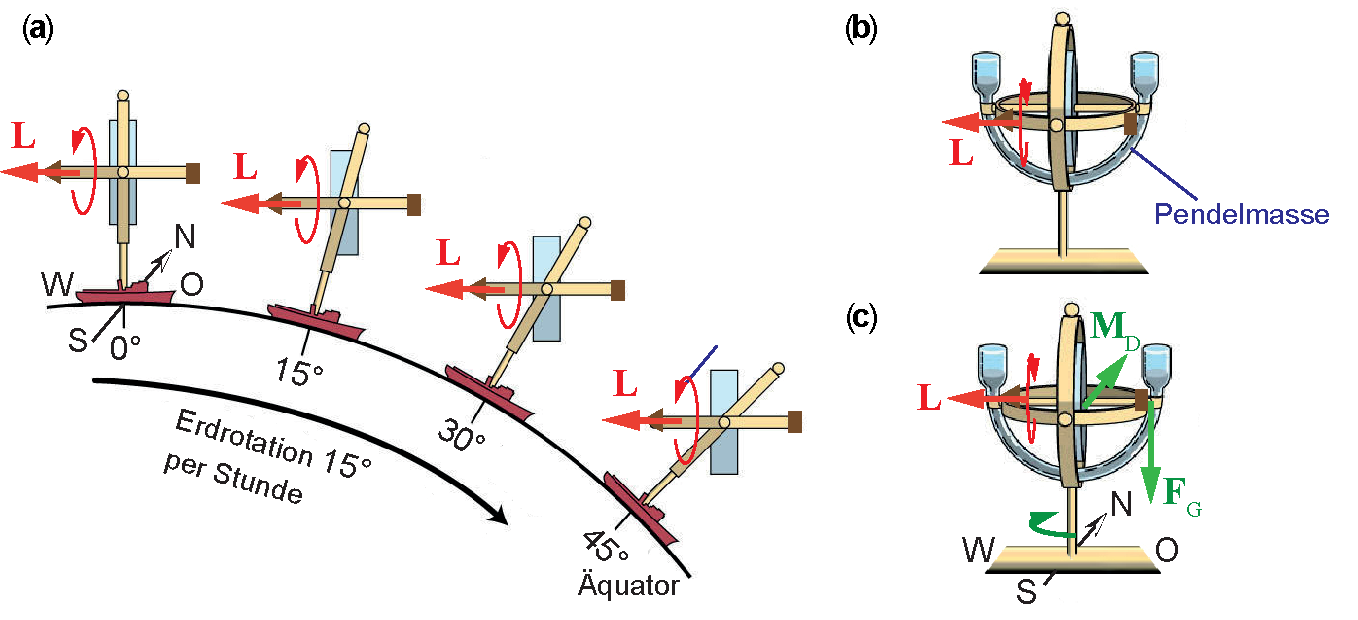
\includegraphics[width=\textwidth]{GyroCompassExpl01.pdf}
\caption[Vergleich freier und Pendelkreisel.]{Vergleich freier und Pendelkreisel. \fa Freier Kreisel auf �quator. \fb Pendelkreisel als Beispiel f�r einen eingeschr�nkten schweren Kreisel. \fc Eine Kraft $\vec{F}_\text{G}$ bewirkt bei einem eingeschr�nkten schweren Kreisel ein Drehmoment $\vec{M}_\text{D}$ in N-Richtung und eine entsprechende Pr�zession. Nach \cite{SFMaritimeNP1946, Britannica2019}.}
\label{abb:bew_GyroCompassExpl01}
\end{figure}

Worin unterscheidet sich nun ein Kreiselkompass von einem frei drehbaren Kreisel? 
Beim Kreiselkompass wird die Bewegung des Kreisels durch die Schwerkraft und eine Zwangsbedingung auf die Horizontebene eingeschr�nkt, \dh die Figurenachse bleibt immer in der Horizontebene liegen, kann sich dort aber frei drehen.
Eine solche Zwangsbedingung kann \zb durch eine entsprechend konstruierte Aufh�ngung (\figref{bew_GyroCompassExpl01}b) realisiert werden.\footnote{Die Designs vieler Kreiselkompasse unterscheiden sich gerade auch in der Realisierung der horizontalen Fixierung.} In diesem Fall haben wir ein sogenanntes Kreiselpendel \index{Kreiselpendel} als Beispiel f�r einen \emph{eingeschr�nkten schweren Kreisel}\index{Kreisel!eingeschr�nkter schwerer}.\\
Wir nehmen nun an, dass dieser Kreisel fest am �quator verankert und seine Rotationsachse in Ost-West-Richtung (O-W) ausgerichtet ist. 
Der Drehimpulsvektor des Kreisels $\vec{L}$ zeigte nach W, was dann der Fall ist, wenn die Eigenrotation des Kreisels bei Blickrichtung von O nach W im Uhrzeigersinn erfolgt (siehe \figref{bew_GyroCompassExpl01}c). 
Die Rotation der Erde von W nach O f�hrt dann dazu, dass aus Sicht eines auf dem Kreisel mitbewegten und in die inititale Westrichtung schauenden Beobachters die Westseite der Horizontebene relativ zur anf�nglich auch im Erdsystem bewegungslosen Kreiselrotationsachse ansteigt, w�hrend die Ostseite absinkt. 
Diese �nderung der Horizontebene bewirkt ein Drehmoment $\vec{M}_\text{D}$ auf den Kreisel.  Man kann sich an Hand von \figref{bew_GyroCompassExpl01}c leicht klar machen, dass dieses Drehmoment parallel zur Erdachse ausgerichtet ist und nach Norden zeigt. Das Drehmoment bewirkt eine Pr�zession des Drehimpulsvektors des Kreisels $\vec{L}$ in Richtung Norden, der Kreisel dreht sich in der Horizontebene im Uhrzeigersinn. Da dieses Drehmoment vom ersten Moment an wirkt und wir annehmen, dass die Pr�zession sofort einsetzt, kommt es in Wirklichkeit nicht zu einer solchen Schr�glage des Kompasses wie in den Stellungen II und III von \figref{bew_GyroCompassExpl02}a gezeigt, sondern der Kreisel ist gezwungernerma�en immer in der Horizontebene ausgerichtet, dreht sich aber in Richtung Norden.\footnote{Wir gehen davon aus, dass bei einer noch so kleinen "`Verkippung"' die "`korrigierende"' Pr�zession instantan erfolgt.}

\begin{figure}
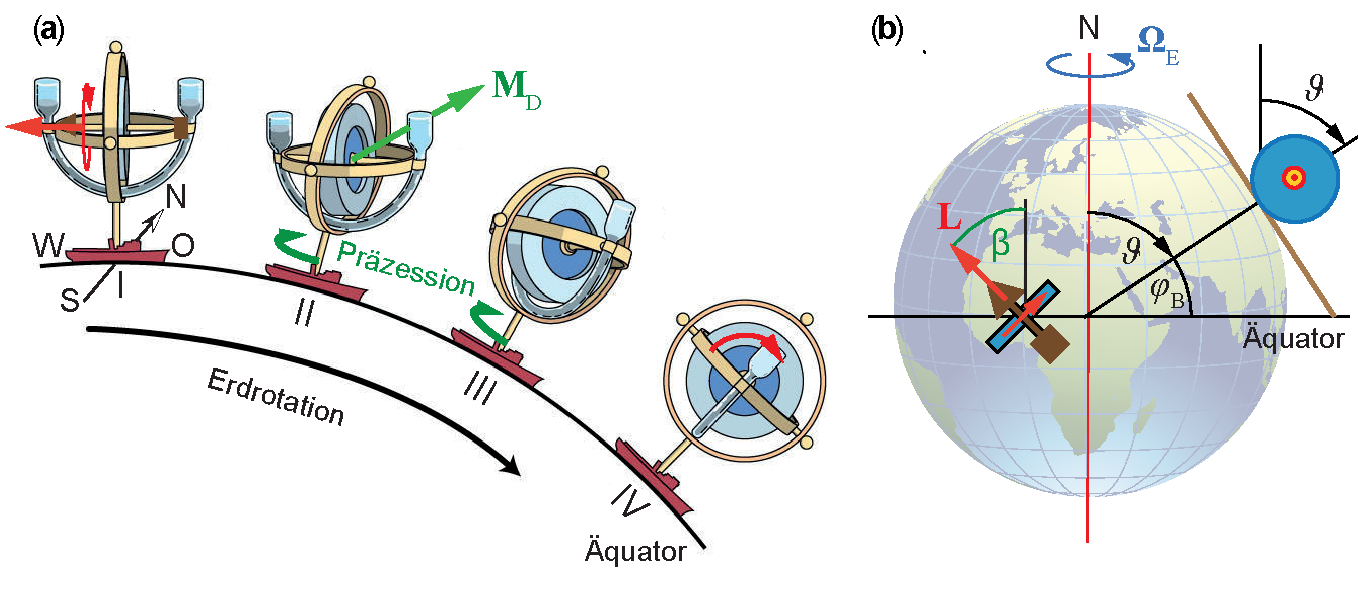
\includegraphics[width=\textwidth]{GyroCompassExpl02.pdf}
\caption[Zum Prinzip des Kreiselkompass.]{Zum Prinzip des Kreiselkompass. \fa Eingeschr�nkter schwerer Kreisel auf der �quator. Ausgangssituation (I), tempor�re virtuelle "`Verkippungen"' (II,III) mit resultierendem Drehmoment und Pr�zessionsrichtung und stabiler Endzustand mit Nordausrichtung (IV). \fb Kreisel auf �quator und Breitengrad. Nach \cite{SFMaritimeNP1946, Rueckner2017,Britannica2019}.}
\label{abb:bew_GyroCompassExpl02}
\end{figure}
Dies passiert bei kontinuierlicher Rotation der Erde solange bis der Kreisel auf Nord-S�d-Richtung ausgerichtet ist (\figref{bew_GyroCompassExpl02}a (IV)). Es kann passieren, dass der Kreisel �ber diesen Punkt ($\vec{M}_\text{D}=0$) hinausl�uft. Dann entsteht ein Gegenmoment $\vec{M}_\text{D} < 0$ und der Kreisel versucht sich wieder nach N  auszurichten. Letztlich wird sich die Kreiselachse bei entsprechender D�mpfung auf die Nord-S�d-Richtung einstellen. Ein solch beschriebener Kreisel wird also durch die Rotation der Erde um ihre Achse so beeinflusst, dass er sich immer nach Norden ausrichtet (daher auch der Name \emph{nordsuchender Kreisel})\footnote{Wir werden gleich sehen, dass der Kreisel sich bei bestimmten Verh�ltnissen mit seinem Eigendrehimpulsvektor auch auf S�den ausrichten kann, in jedem Fall richtet er sich auf die Nord-S�d-Linie (Meridian) aus.} und im Gegensatz zum magnetischen Kompass exakt zum geographischen und nicht zum magnetischen Nordpol ausgerichtet ist.\\
Befindet sich der Kreisel nicht am �quator, sondern auf einem Breitengrad $\varphi_\text{B} = 90\degree - \vartheta$, dann ist die Horizontebene um 
den Winkel $\varphi_\text{B}$ gegen�ber der Erdrotationsachse geneigt (\figref{bew_GyroCompassExpl02}b) und das Drehmoment $\vec{M}_\text{D}$ ist um den Faktor $\cos\varphi_\text{B} = \sin\vartheta$ verkleinert und wird mithin am Nordpol Null. Kreiselkompasse k�nnen also am Pol nicht funktionieren.\\

\textbf{Berechnung der Dynamik des nordsuchenden Kreisels}\\

Wir wollen uns nun den schematischen Aufbau eines Kreiselkompasses nach \figref{bew_KreiselkompSchematisch}a anschauen. Im Gegensatz zum oben skizzierten Pendelkreisel (\figref{bew_GyroCompassExpl01}b) haben wir hier die Situation, dass die konstante Lage der Kreiselachse (Figurenachse) in der Horizontebene durch eine schwimmende Lagerung realisiert wird. Durch diese Lagerung kann sich die Kreiselachse frei in den horizontalen Richtungen $x, y$ drehen.
Der Schwerpunkt des S des Kreisels befindet sich jedoch unter dem
geometrischen Mittelpunkt A der Anordnung, an welcher der Auftrieb angreift. 
Wir haben es deshalb auch hier mit einem (eingeschr�nkten) schweren Kreisel\index{Kreisel!schwerer} zu tun, der sich 
aufgrund der Schwerkraft mit seiner Figurenachse �hnlich dem Pendelkreisel immer in der Horizontebene ausrichten wird (\figref{bew_KreiselkompSchematisch}b).

\begin{figure}
  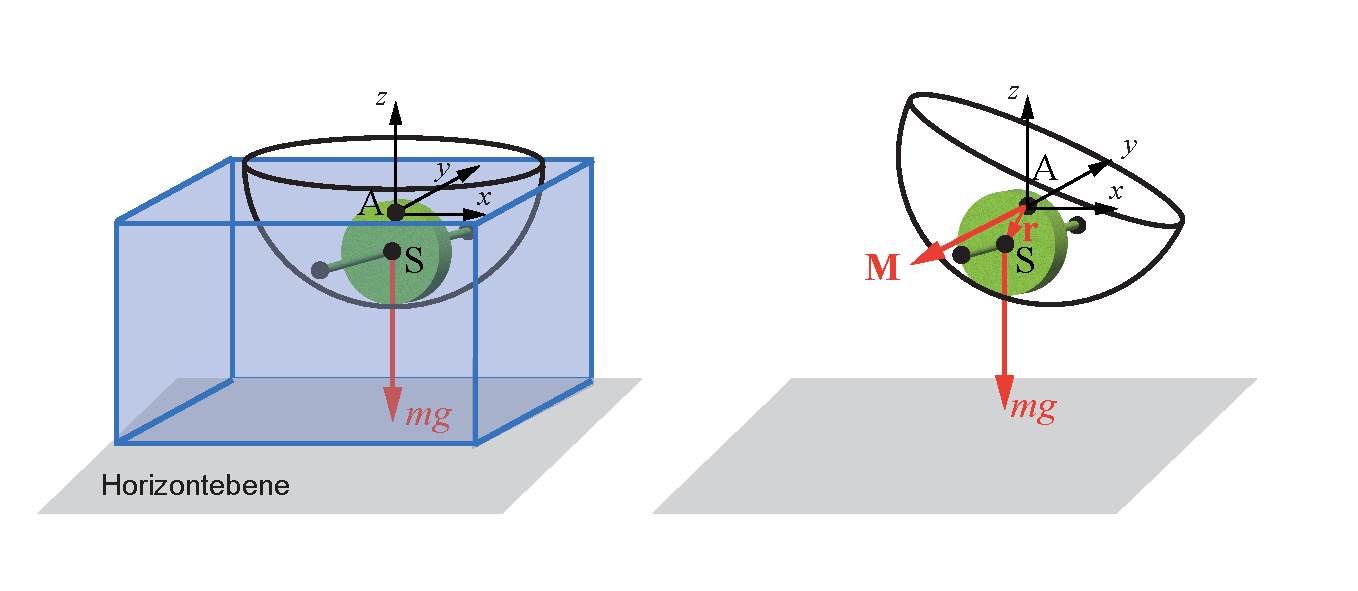
\includegraphics[width=\textwidth]{KreiselkompAufbau.pdf}
  \caption[Schematischer Aufbau des Kreiselkompasses.]{Schematischer Aufbau des
    Kreiselkompasses. Der Kreisel ist hier schwimmend derart gelagert,
    dass die Figurenachse immer in der horizontalen Ebene zu liegen kommt. Dies
    wird durch die Gewichtskraft bewirkt, denn der Schwerpunkt ist unterhalb
    des geometrischen Mittelpunkts des schwimmenden Geh�uses A, an dem der
    Auftrieb angreift, angeordnet. Dies bewirkt sofort ein korrigierendes
    Drehmoment $\vec{M}_\text{D}$, falls eine Auslenkung aus der horizontalen Ebene
    heraus auftreten sollte. In der horizontalen Ebene kann die Figurenachse
    frei rotieren.}
    \label{abb:bew_KreiselkompSchematisch}
\end{figure}

Wie beschrieben entsteht durch �nderung der Richtung der Schwerkraft aufgrund der Rotation der Erde ein Drehmoment, das eine Drehimpuls�nderung zur Folge hat. Die Drehimpuls�nderung erfolgt nur als Rotation um den Punkt A in der horizontalen Ebene. \\

F�r die Berechnung der Dynamik, wie sich ein solcher eingeschr�nkter Kreisel nach Norden
ausrichtet, betrachten wir den Kreisel im Nichtinertialsystem\index{Nichtinertialsystem} der rotierenden Erde. 
Man muss f�r die Aufstellung der Lagrange-Funktion\index{Lagrange-Funktion} alle Rotationen, \dh alle
Drehimpulse, zus�tzlich zum im Inertialsystem betrachteten Eigendrehimpuls, ber�cksichtigen. 
Insbesondere muss der Drehimpuls aufgrund der Rotation der Erde
hinzuaddiert werden.\footnote{Siehe
\zb \cite{Mueller2020} f�r eine ausf�hrliche Betrachtung.}

F�r die entstehende komplizierte Bewegung des Kreisels 
betrachten wir alle m�glichen Drehbewegungen im \textit{k�rperfesten Hauptachsensystem} \index{Hauptachsensystem} und 
setzen dieses in Bezug zu einem raumfesten Koordinatensystem (Inertialsystem).
Die einzelnen, sich �berlagernden, Drehbewegungen werden nun schrittweise
eingef�hrt.\footnote{Es w�rde sich auf den ersten Blick anbieten,
  wieder auf die Eulerwinkel oder zumindest �hnliche Definitionen 
  zur�ckzugreifen, um die Bewegung zu beschreiben.
  Da wir jetzt jedoch explizit ber�cksichtigen m�ssen, dass das mit der
  Erde verbundene Koordinatensystem kein Inertialsystem ist und die Bewegungen
  aufgrund der Einschr�nkung auf eine Ebene komplizierter ausfallen, sind die
  Euler-Winkel hier weniger geeignet. Um eine Verwechslung zu vermeiden, f�hren wir
  neue Bezeichnungen $(\alpha,\,\beta,\,\vartheta)$ ein.} 

\begin{figure}
  \includegraphics[width=\textwidth]{KreiselkompKS.pdf}
  \caption[Koordinatensysteme f�r den Kreiselkompass.]{Koordinatensysteme f�r
    den Kreiselkompass. \fa Ber�cksichtigung der Erddrehung f�r einen
    Kreiselkompass am Nordpol. \fb Auf dem Breitengrad, auf
    dem sich der Kompass nun befindet, soll die $z''$-Achse zum Zenit zeigen. \fc
    Bewegung des Kreiselkompasses in der Horizontebene mit freiem
    Drehwinkel $\beta$. \fd Schnelle Rotation um die Figurenachse $x'''= x''''$,
    ausgedr�ckt durch den Winkel $\alpha$.}
    \label{abb:bew_KreiselkompKS}
\end{figure}

Das k�rperfeste Koordinatensystem des Kreiselkompasses der Halbkugel in \figref{bew_KreiselkompSchematisch} (es wird nachstehend das System $\vec{K}'''$ sein) muss deren Orientierung immer relativ zu dem Ort beschreiben,
an dem sich der Kompass befindet. Dann k�nnen wir aus dieser Beschreibung Navigationsinformationen ablesen. 
Wir beginnen mit dem raumfesten Koordinatensystem $\vec{K}$. 
Im ersten Schritt zum �bergang in das k�rperfeste Koordinatensystem 
ber�cksichtigen wir eine Drehung um die
$z$-Achse, um der Drehung der Erde zu folgen. Es ergibt sich
das Koordinatensystem $\vec{K}'$ (siehe \figref{bew_KreiselkompKS}~a). 
Der Ort des ortsfesten Kreisels liegt auf einem festen Breitengrad, das Koordinatensystem wird so
gew�hlt, dass die $z''$-Achse des Koordinatensystems $\vec{K}''$ 
dort zum Zenit zeigt. Die Transformation erfolgt durch eine
Drehung um die $x'$-Achse (\figref{bew_KreiselkompKS}~b). Der Kompass
kann sich nun um die $z''$-Achse frei bewegen. Dies soll durch den Winkel
$\beta$ ausgedr�ckt werden (\figref{bew_KreiselkompKS}~c). Schlie�lich
muss in einem k�rperfesten System (Koordinatensystem $\vec{K}''''$)
noch ber�cksichtigt werden, dass die schnelle
Rotation des Kreisels um die $x'''$-Achse zu einer Ver�nderung der Achsen
$y'''$ und $z'''$ f�hrt. Die schnelle Rotation wird durch den Winkel $\alpha$
beschrieben (\figref{bew_KreiselkompKS}~d). 

Zun�chst wollen wir uns mit dem Fall besch�ftigen, dass der Kreiselkompass
fest an einem Punkt auf der Erdoberfl�che steht. Das hei�t, dass $\vec{\Omega}_\text{E}$
immer exakt der Rotation der Erde um ihre Achse entspricht (also keine
Bewegung entlang eines Breitengrades erfolgt) und $\vartheta$ ein
unver�nderlicher Winkel ist (also keine Bewegung entlang eines L�ngengrades
erfolgt). Sp�ter werden wir auf bewegte Objekte wie Schiffe und Flugzeuge
eingehen.

Zur Figurenachse $x'''=x''''$ geh�rt das Haupttr�gheitsmoment $J_1$. Die
beiden dazu senkrechten, identischen Tr�gheitsmomente bezeichnen wir mit
$J_{23}$. \\
Dann lauten die einzelnen Drehbewegungen ausgedr�ckt durch die $\vec{\omega}_{\alpha,\beta,\text{E}}$ wie folgt:
\begin{itemize}
\item Die schnelle Rotation des Kreisels um seine Haupttr�gheitsachse $x''''$
  mit dem Winkel $\alpha$ ist zu ber�cksichtigen.
  Die zugeh�rige Winkelgeschwindigkeit
  ist bereits im k�rperfesten System gegeben:
  \begin{equation*}
    \vec{\omega}_\alpha'''' = \begin{pmatrix} \dot{\alpha}\\ 0 \\ 0
    \end{pmatrix} \,.
  \end{equation*}
\item Die freie Bewegung der Figurenachse in der horizontalen Ebene wird
  durch den Winkel $\beta$ ausgedr�ckt. Dies entspricht in der schematischen
  Zeichnung aus \figref{bew_KreiselkompSchematisch} einer Drehung um den
  Punkt A mit dem Winkel $\beta$. Im k�rperfesten System m�ssen wir
  ber�cksichtigen, dass sich die Lage der Drehachse durch die Rotation mit
  $\vec{\omega}_\alpha''''$  st�ndig �ndert. Die Winkelgeschwindigkeit erh�lt
  hier also unter Ber�cksichtigung der Transformation $\vec{K}''' \Rightarrow \vec{K}''''$ den Wert
  \begin{equation*}
    \vec{\omega}_\beta'''' = \begin{pmatrix} 1 & 0 & 0 \\ 0 & \cos\alpha
      & \sin \alpha \\ 0 & -\sin \alpha & \cos\alpha \end{pmatrix}
    \begin{pmatrix} 0 \\ 0 \\ \dot{\beta} \end{pmatrix}
    = \begin{pmatrix} 0 \\ \sin \alpha \, \dot{\beta} \\ \cos\alpha
      \dot{\beta} \end{pmatrix} \,.
  \end{equation*}
\item Schlie�lich muss noch die Drehung der Erde ber�cksichtigt werden.
  Mit der Lage des k�rperfesten Koordinatensystems entsprechend
  \figref{bew_KreiselkompKS} muss man insgesamt drei Rotationen beachten, 
	$\vec{K}' \Rightarrow \vec{K}''$, dann $\vec{K}'' \Rightarrow \vec{K}'''$ 
	und zum Schluss $\vec{K}''' \Rightarrow \vec{K}''''$, 
  um die Erdachse im k�rperfesten System angeben zu k�nnen:
  \begin{align*}
    \vec{\omega}_\text{E}'''' &= \mathbb{R}_x(\alpha)\, \mathbb{R}_z(\beta)\,\mathbb{R}_y(\vartheta)\,\vec{\Omega}_E \, = \, \begin{pmatrix} 1 & 0 & 0 \\ 0 & \cos\alpha
      & \sin \alpha \\ 0 & -\sin \alpha & \cos\alpha \end{pmatrix}
    \begin{pmatrix} \cos\beta & \sin \beta & 0 \\ -\sin\beta &
      \cos\beta & 0 \\ 0 & 0 & 1 \end{pmatrix}
    \begin{pmatrix} \cos\vartheta & 0 & -\sin\vartheta \\ 0 & 1 & 0 \\
      \sin\vartheta & 0 & \cos\vartheta \end{pmatrix}
    \begin{pmatrix} 0 \\ 0 \\ \Omega_\text{E} \end{pmatrix} \\
    &= \begin{pmatrix} -\sin\vartheta \cos\beta \, \Omega_\text{E} \\
      \left ( \sin \vartheta \sin \beta \cos\alpha + \cos\vartheta
        \sin\alpha \right ) \Omega_\text{E} \\
      \left ( -\sin\vartheta \sin\beta \sin\alpha + \cos\vartheta
        \cos \alpha \right ) \Omega_\text{E} 
    \end{pmatrix}\,.
  \end{align*}
  Dabei ist $\Omega_\text{E}$ die Rotationsgeschwindigkeit der Erde.
\end{itemize}
Der resultierende Vektor der Winkelgeschwindigkeit im k�rperfesten System
lautet damit
\begin{align}
  \vec{\omega}'''' &=\begin{pmatrix} {\omega_1}'''' \\ {\omega_2}''''\\ {\omega_3}'''' \end{pmatrix} 
	= \vec{\omega}_\alpha'''' + \vec{\omega}_\beta''''  + \vec{\omega}_\text{E}''''\nonumber \\
	&= \begin{pmatrix} \dot{\alpha} -\sin\vartheta \cos\beta\, \Omega_\text{E}\\
    \sin\alpha \, \dot{\beta} + \left ( \sin\vartheta \sin\beta \cos\alpha
      + \cos\vartheta \sin\alpha \right ) \Omega_\text{E} \\
    \cos\alpha \, \dot{\beta} + \left ( -\sin\vartheta \sin\beta \sin\alpha
      + \cos\vartheta \cos\alpha \right ) \Omega_\text{E} \end{pmatrix} \; .
  \label{eq:bew_WinkelgeschKreiselkompass}
\end{align}
Da wir im Haupttr�gheitsachsensystem sind, ergibt sich die kinetische
Energie dieses Kreisels einfach aus den Diagonalelementen zu 
\begin{align}
  T & = \frac{1}{2} \sum_i^3 \, J_i\, (\omega_i{''''})^2 \nonumber = \frac{J_1}{2} \omega_1''''^2 + \frac{J_{23}}{2} \left ( \omega_2''''^2 +
    \omega_3''''^2 \right )\nonumber \\
		&= \frac{J_1}{2} \left ( \dot{\alpha} -\sin\vartheta \cos\beta \, \Omega_\text{E}
  \right )^2 \nonumber \\
	 &~~~+ \frac{J_{23}}{2} \left \{ \dot{\beta}^2 + 2 \cos\vartheta \, \Omega_\text{E} \, \dot{\beta} + \left ( \sin^2\vartheta \sin^2\beta + \cos^2\vartheta
    \right ) \Omega_\text{E}^2 \right \} \;. \label{eq:bew_Lagrange_KK01}
\end{align}

Die Wirkung der Schwerkraft haben wir bereits derart ber�cksichtigt,
dass wir nur freie Rotationen um die Winkel $\alpha$ und $\beta$ zulassen, 
die damit die f�r das Problem die geeigneten generalisierten Koordinaten sind.
Die Schwerkraft erzwingt, wie oben erw�hnt, dass der Kreisel immer
in einer horizontalen Ebene aufgeh�ngt ist. Wir gehen weiter davon aus, dass sich
diese horizontale Lage so schnell einstellt, dass sie auch bei einer Bewegung
des Kreisels immer gegeben ist. Auf die verbleibenden Rotationen hat die
Schwerkraft dann keinen Einfluss und somit tritt in dieser Bewegung kein
Potential auf $(U=0)$. Die Lagrange-Funktion ist daher mit der kinetischen Energie
identisch, $\mathcal{L} = T$.\\
Ferner findet man, dass $\alpha$ wegen $\d \mathcal{L}/ \d \alpha = 0$ eine
zyklische Koordinate ist. Die zugeh�rige Erhaltungsgr��e
\begin{equation*}
  \frac{\partial \mathcal{L}}{\partial \dot{\alpha}} = J_1 \, \lk 
  \dot{\alpha} -\sin\vartheta \cos\beta \, \Omega_\text{E} \rk = L_1'''' = \con
\end{equation*}
ist nichts anderes als die $x''''$-Komponente des Drehimpulses im k�rperfesten
System. Nicht erhalten wird jedoch die Winkelgeschwindigkeit $\dot{\alpha}$.
Dies muss so sein, weil je nach Lage des Kreisels, also je nach dem Wert der
Winkel $\beta$ und $\vartheta$, die Komponente der Erdrotation entlang der
$x''''$-Achse gr��er oder kleiner ist. Die schnelle Rotation $\dot{\alpha}$ muss sich also 
beschleunigen oder abbremsen, um die Drehimpulskomponente erhalten zu k�nnen.

F�r den Winkel $\beta$ ergibt sich aus den Lagrange-Gleichungen die Bewegungsgleichung
\begin{align}
  0 &= \frac{\D}{\D t}\frac{\partial \mathcal{L}}{\partial \dot{\beta}} -
      \frac{\partial \mathcal{L}}{\partial \beta} = J_{23} \ddot{\beta} -
      L_1'''' \sin\vartheta \sin \beta \; \Omega_\text{E} - J_{23}\sin^2\vartheta
      \cos\beta \sin \beta \; \Omega_\text{E}^2 \nonumber \\
      \text{\bzw} ~~ \ddot{\beta} &= \left ( \frac{L_1''''}{J_{23}} \sin\vartheta \; \Omega_\text{E} \:
                     + \:\sin^2\vartheta \; \Omega_\text{E}^2 \cos\beta
                     \right ) \sin \beta \; . \label{eq:bew_Lagrange_KK02}
\end{align}
Es gibt offensichtlich zwei Ruhelagen $(\ddot{\beta} =0)$, n�mlich $\beta = 0$ und $\beta = \pi$.
Nur eine davon ist jedoch stabil. Welche das ist, h�ngt von der
Drehimpulskomponente $L_1''''$ ab. Da wir davon ausgehen, dass der Kreisel
schnell um seine Figurenachse rotiert, also $\dot{\alpha} \gg \Omega_\text{E}$,
dominiert $L_1'''' \approx J_1\, \dot{\alpha}$ die Bewegungsgleichung und entscheidet zusammen mit
$\sin\beta$ �ber das Vorzeichen von $\ddot{\beta}$. Wenn wir ber�cksichtigen,
dass der Winkel $\beta$ die Rotation der Figurenachse ($x'''=x''''$) gegen die
Nordrichtung beschreibt (siehe \figref{bew_KreiselkompKS}), so
ergeben sich zwei M�glichkeiten.
\begin{itemize}
\item Der Kreisel rotiert von oben gesehen in positiver Richtung um die Figurenachse
  ($\dot{\alpha} > 0)$: In diesem Fall ist $\beta = \pi$ die stabile
  Ruhelage, um die herum der Kreisel eine R�ckstellkraft erf�hrt. Die
  Figurenachse ist "`s�dsuchend"'.
\item Der Kreisel rotiert von oben gesehen in negativer Richtung um die Figurenachse
  ($\dot{\alpha} < 0)$: In diesem Fall ist $\beta = 0$ die stabile
  Ruhelage. Die Figurenachse ist "`nordsuchend"'.
\end{itemize}
In jedem Fall schwingt jedoch die Figurenachse um die Nord-S�d-Richtung und
der Kreiselkompass identifiziert diese. D�mpft man diese Schwingungsbewegung,
was in einem realen Aufbau eines Kreiselkompasses immer der Fall ist, kommt
diese Schwingung in ihrer Ruhelage zum Erliegen. Sp�testens dann ist die
Nord-S�d-Richtung zuverl�ssig markiert. 

Die Ausrichtung im Schwerefeld geschieht in einem Kreiselkompass durch
Lagerung in einer Fl�ssigkeit. Diese bewirkt die D�mpfung der Bewegung
im Winkel $\beta$. Wir gehen in unserer Modellbildung daher von einer zur 
Geschwindigkeit proportionalen D�mpfung aus und erg�nzen diese in der
Bewegungsgleichung f�r $\beta$. Damit erhalten wir
\begin{equation}
  \ddot{\beta} = \left ( \frac{L_1''''}{J_{23}} \sin\vartheta \; \Omega_\text{E} 
    + \sin^2\vartheta \; \Omega_\text{E}^2 \cos\beta \right ) \sin \beta
  - \gamma \dot{\beta}
  \label{eq:bew_KreiselkompassGedaempft}
\end{equation}
mit der D�mpfungskonstanten $\gamma$. Diese Gleichung muss numerisch gel�st
werden, was wir in \probref{bew_gedaempfterKreiselkompass} angehen.

Aber auch diese Betrachtung gilt weiterhin nur f�r einen Kreiselkompass, der
fest auf einem Punkt der Erdoberfl�che steht. Bewegt sich dieser, hat das
einen Einfluss auf die Ausrichtung der Figurenachse. Wir wollen dazu die
Bewegung eines Schiffes oder Flugzeugs, auf dem sich der Kreiselkompass bewegt,
in zwei Komponenten aufteilen.
\begin{itemize}
\item Eine Bewegung entlang eines Breitengrades entspricht einer Vergr��erung oder Verkleinerung
  der Winkelgeschwindigkeit $\Omega_\text{E}$, da die Bewegung in exakt dieselbe
  Richtung erfolgt. Auf die Ausrichtung der Ruhelage der Figurenachse hat dies
  keinen Einfluss. Jedoch ergibt sich aus Gleichung
  \eqref{eq:bew_KreiselkompassGedaempft} ein Einfluss auf die Bewegung des
  Kreisels w�hrend der Phase des Einstellens auf die Nord-S�d-Richtung und damit
  der Zeit, bis der Kreiselkompass zur Ruhe kommt.
\item Eine Bewegung entlang eines L�ngengrades resultiert in einem
  zeitlich ver�nderlichen Winkel $\vartheta$. Nimmt man eine Bewegung mit einer
  festen Geschwindigkeit $v$ an, resultiert dies in einer (festen)
  Winkelgeschwindigkeit $\dot{\vartheta} = v/a$ mit dem Abstand $a$ zum
  Erdmittelpunkt (f�r ein Schiff gilt in etwa $a=R_\text{E}$ (Erdradius)). Dieser Fall
  hat eine Missweisung der Nord-S�d-Richtung zur Folge, die auch \textit{Fahrtfehler} genannt wird und 
in \probref{bew_KreiselkompassLaengenkreis} genauer untersucht wird. Ebenso analysieren wir in der �bung das Verhalten des 
Kreiselkompass (und damit seine Empfindlichkeit) gegen�ber St�rbeschleunigungen.
\end{itemize}


\subsection{Pr�zession der Erde} \index{Pr�zession!der Erde} \label{kap:bew_praez_erde}

Die Pr�zession des Erdkreisels spielt in der Astronomie
und in der Himmelsmechanik (Band II, Kapitel 3) eine wichtige Rolle.
Schon der griechische Astronom der Antike Hipparchos\indexp{Hipparchos}%
\footnote{Hipparchos von Nic�a (190~v.~Chr.--120~v.~Chr.) war der bedeutendste Astronom seiner Zeit. Er gilt als Begr�nder der wissenschaftlichen Astronomie und erzielte bei seinen Beobachtungen eine erstaunliche Genauigkeit. So konnte er die Erdpr�zession ziemlich genau messen und bestimmte auch die Dauer des tropischen Jahres. Sein Wert weicht nur 6.5 Minuten vom heute gemessenen Wert ab.}
wusste, dass die Erdachse pr�zediert.
Da die Erde in etwa ein Rotationsellipsoid%
\footnote{W�re die Erde eine perfekte Kugel, g�be es keine Pr�zession.}
ist, bewirkt seine �quatorwulst im Zusammenspiel mit den von den Gezeitenkr�ften von Sonne und Mond
erzeugten Drehmomenten eine sogenannte \emph{lunisolare Pr�zession}\index{Pr�zession!lunisolare}.
Wir k�nnen f�r die Berechnung der Pr�zession das Erdellipsoid
in guter N�herung als schweren, abgeflachten (\textit{oblaten})
Kreisel\index{Kreisel!oblater} betrachten (\figref{bew_Erdpraezession}),
f�r den $\Delta J = J_{12}-J_3 = J - J_3 < 0$ gilt.
F�r die Erde berechnet sich nach \probref{bew_traegheitsmomente} das Verh�ltnis $\Delta J/J_{3}$ ungef�hr zu
        \begin{align*}
            \frac{\Delta J}{J_{3}}\approx \frac{1}{300} \,.
        \end{align*}

\begin{figure}
  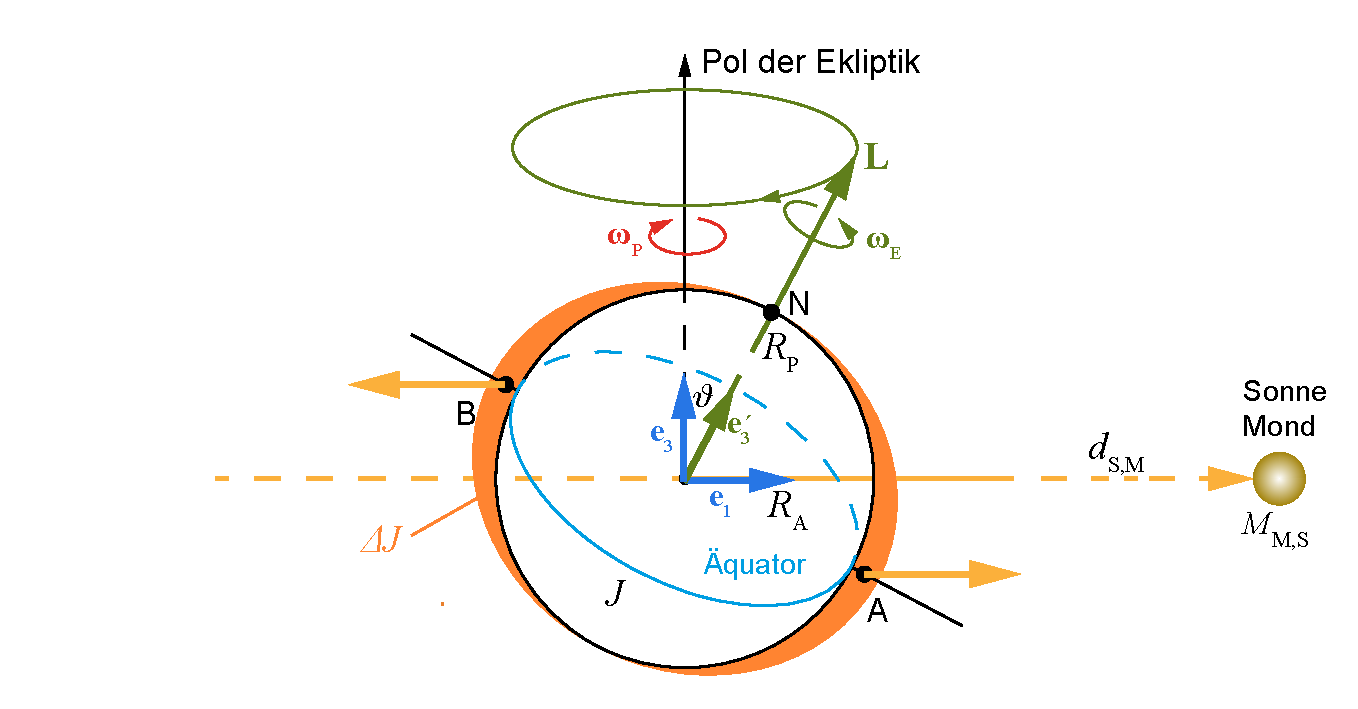
\includegraphics[width=\textwidth]{ErdPraezession01.pdf}
  \caption[Pr�zession der Erde durch Gezeitenkr�fte von Sonne und Mond.]{Pr�zession der Erde durch Gezeitenkr�fte von Sonne und Mond.}
    \label{abb:bew_Erdpraezession}
\end{figure}

Das von Sonne und Mond bewirkte Drehmoment auf die Erdachse (\figref{bew_Erdpraezession}) kann in guter N�herung wie folgt berechnet werden, siehe auch \cite{Bartelmann2015, Montenbruck2012} und \probref{bew_DrehmomentPraezErde}: \\
        \begin{align}
            \begin{split}
                \vec{M}_\text{S} &= \frac{3G\,m_\text{S}}{2{d_\text{S}}^3}\,\cos\vartheta\,\Delta J\,\lk \vecpeZ\times\veceZ \rk = C_\text{S}\,\lk \vecpeZ\times\veceZ \rk\,, \\
                \vec{M}_\text{M} &=  \frac{3G\,m_\text{M}}{2{d_\text{M}}^3}\,\cos\vartheta\,\Delta J\,\lk \vecpeZ\times\veceZ \rk = C_\text{M}\,\lk \vecpeZ\times\veceZ \rk \,. \label{eq:bew_ErdPraezess01}
            \end{split}
        \end{align}
Hierin sind $m_\text{S}, m_\text{M}$ die Massen von Sonne und Mond, $d_\text{S}, d_\text{M}$ die Abst�nde der Himmelsk�rper vom Erdmittelpunkt und $\vartheta$ der Neigungswinkel der Erdachse zur Bahn. $\vecpeZ$ ist der Achsenvektor im mitbewegten System der Erde und $\veceZ$ der Normalenvektor der \textit{Ekliptik} (Erdbahnebene)\index{Ekliptik}. Wir haben hierbei angenommen, dass der Mond sich ebenfalls in dieser Ebene bewegt. In \figref{bew_Erdpraezession} sind die Gezeitenkr�fte eingezeichnet, die auf die �quatorwulst wirken. Das resultierende Moment w�rde die Erdachse aufrichten, wenn die Erde kein rotierender Kreisel w�re.\\
Wie man in \eqref{eq:bew_ErdPraezess01} an der $d_\text{S,M}{}^{-3}$-Abh�ngigkeit erkennen kann, werden diese Drehmomente durch Gezeitenkr�fte (siehe \kap{bew_gezeiten}) hervorgerufen. In \probref{bew_DrehmomentPraezErde} werden wir das im Detail zeigen und auch \eqref{eq:bew_ErdPraezess01} herleiten. Wir wollen noch in sehr guter N�herung annehmen, dass die Figurenachse der Erde mit der Drehimpulsachse zusammenf�llt, dass also $ \vec{L} = L\,\vecpeZ$ gilt. Dann folgt aus der Bewegungsgleichung f�r den starren K�rper
        \begin{align}
            \frac{\D \vec{L}}{\D t} = \vec{M}_\text{M} + \vec{M}_\text{S} \label{eq:bew_ErdPraezess02}
        \end{align}
sofort eine Beziehung f�r das Betragsquadrat des Drehimpulses
        \begin{align}
           \frac{1}{2}\,\frac{\D L^2}{\D t} &= \vec{L}\,\frac{\D \vec{L}}{\D t} = L\,\vecpeZ\,\cdot\,\lk \vec{M}_\text{M} + \vec{M}_\text{S}\rk \approx L\,\underbrace{\vecpeZ\,\cdot\,\lk \vecpeZ\times \veceZ\rk\lk C_\text{S} + C_\text{M} \rk }_{\substack{=0}} \,. \label{eq:bew_ErdPraezess02a}
        \end{align}
Das hei�t, durch das Drehmoment der Gezeitenkr�fte kann sich
in unserem Modell nur die Richtung des Erddrehimpulses �ndern,
nicht aber sein Betrag.
Die Gezeitenkr�fte bewirken in unserem Fall des starren Rotationsellipsoiden also \emph{keine} Abbremsung
der Erdrotation, im Gegensatz zu einem anderen Modell einer teilweisen
nichtstarren Erde, das zum Effekt der Gezeitenreibung f�hrt (siehe auch Band II, Kapitel 3).\\
Wir wollen nun die Pr�zessionsfrequenz bestimmen. \\
Aus \eqref{eq:bew_ErdPraezess02} findet man mit $\vec{L} = L\,\vecpeZ$
        \begin{align*}
            \frac{\D \lk L\,\vecpeZ\rk}{\D t} &= J_3\, \omega_\text{E} \frac{\D \lk \vecpeZ\rk}{\D t} = L \vec{\omega}_\text{P} \times \vecpeZ = - L \vecpeZ \times \vec{\omega}_\text{P}  = -J \, \omega_\text{E} \, \omega_\text{P} \,\lk \vecpeZ \times \veceZ\rk \\
						&= \frac{3G\,\cos\vartheta\,\Delta J }{2}\lk \frac{m_\text{S}}{{d_\text{S}}^3}+\frac{m_\text{M}}{{d_\text{M}}^3}\rk \, \lk \vecpeZ\times \veceZ \rk \,.
 					\end {align*}
        \begin{align}
          \rightarrow \,\, \vec{\omega}_\text{P} &= - \underbrace{\frac{3G\,\cos\vartheta\,\Delta J }{2\, J_3\,\omega_\text{E}}\lk \frac{m_\text{S}}{{d_\text{S}}^3}+\frac{m_\text{M}}{{d_\text{M}}^3}\rk}_{= \left|\vec{\omega_\text{P}}\right| = \omega_\text{P}}\,\veceZ \label{eq:bew_ErdPraezess03}
        \end{align}
In \eqref{eq:bew_ErdPraezess03} erkennen wir $\omega_\text{P} = M/L$ aus \eqref{eq:bew_SchwererKr02} wieder.
Mit den bekannten Werten $\vartheta \approx \SI{23.45}{\degree}$, $m_\text{S} = \SI{1.98e30}{\kg}$, $m_\text{M} = \SI{7.35e22}{\kg}$, $d_\text{S} = \SI{1.49e11}{\metre}$, $d_\text{M} = \SI{3.84e8}{\metre}$ und $\omega_\text{E} = 2\pi/(\SI{86125}{\second})$ ergibt sich insgesamt 
        \begin{align*}
            \omega_\text{P} = \SI{7.94e-12}{\per\second} ~~~~ \text{oder} ~~~~ T_\text{P} = \frac{2\pi}{\omega_\text{P} } \approx 25\,100\,\text{Jahre}\,,
        \end{align*}
was sehr gut mit den astronomisch beobachteten 25\,800 Jahren �bereinstimmt.
Es sei bemerkt, dass die Beitr�ge von Mond und Sonne sich wie 2.2 : 1 verhalten. Das gleiche Verh�ltnis hatten wir bei den Gezeiten gefunden, was nicht verwunderlich ist, da f�r das Drehmoment der Pr�zession ja die Gezeitenkr�fte verantwortlich sind. F�r eine vertiefte Betrachtung empfehlen wir auch die Ref. \cite{Rainey2022}, die auch die Konsequenzen dieser Pr�zession der Erdachse auf das Langzeitverhalten unseres Klimas beleuchtet. Wir werden das ebenfalls mit einer etwas vereinfachten Methode im Kapitel Himmelsmechanik im Band II, Kapitel 3 tun. 
Eine genauere Untersuchung der Bewegung der Erdachse zeigt im �brigen, dass diese auch noch kleinere und kurzperiodischere (ca.\ 18--19 Jahre) nick�hnliche Bewegungen macht, die als 
\emph{astronomische} Nutation\index{Nutation!astronomische}
bezeichnet werden. 
Es sei darauf hingewiesen, dass der Begriff der astronomischen
Nutation nicht identisch ist mit dem in \autoref{kap:bew_starrer_koerper}
definierten Begriff der Nutation in der Kreiseltheorie.
Die astronomische Nutation als relativ schnell schwankender,
aber viel kleinerer Teil der Pr�zession der Erdachse ist also
selbst eine Pr�zession, die vor allem von der Pr�zession
der Mondbahn hervorgerufen wird.%
\footnote{Auch das Mond-Erde-System kann man als Kreisel betrachten,
der im Schwerefeld der Sonne pr�zediert.}
Als Folge dieser beiden genannten Richtungs�nderungen
der Erdachse ver�ndern sich nat�rlich auch die Koordinaten
der Sterne �ber die Zeit. Die Pr�zession der Erde war schon mehr als anderthalbtausend Jahre bekannt, bevor die astronomische Nutation der Erdachse 1728 von James Bradley\footnote{James Bradley\indexp{Bradley, James} (1693--1762) war ein englischer Astronom. Er gilt als einer der Pioniere der Astrometrie\index{Astrometrie} und wies die Bewegung der Erde um die Sonne durch die j�hrliche Aberration\index{Aberration} der Gestirne nach.} entdeckt wurde. Die Ursache dieser astronomischen Nutation konnte man dann aber erst 20 Jahre sp�ter auf Basis der oben beschriebenen Theorie des starren K�rpers erkl�ren.

\subsection{Trebuchet}\label{kap:bew_trebuchet}

\begin{figure}
\includegraphics[width=\textwidth]{Blide01.pdf}
\caption[Mittelalterliche Wurfmaschine und Prinzip der Funktionsweise.]{Nachbau (links) und Funktionsweise (rechts)  einer mittelalterlichen Steinschleuder (Trebuchet, Blide).}\label{abb:bew_Blide01}
\end{figure}

Zum Schluss des Kapitels Physik der Bewegung von K�rpern wollen wir uns noch ein besonderes Highlight g�nnen und eine mittelalterliche Steinschleuder behandeln.
Hierbei k�nnen wir fast alles Gelernte anwenden, insbesondere die Erhaltungss�tze, Zwangsbedingungen, Lagrange-Multiplikatoren und Lagrange-Gleichungen erster und zweiter Art, sowie numerische L�sungen mit ODE- und DAE-Solvern von \matlab.\\
Die Steinschleuder (\figref{bew_Blide01}) war im Mittelalter eine der gr��ten und zugleich genauesten Wurfwaffen mit ungeheuerlicher Durchschlagskraft und relativ gro�er Reichweite. 
H�ufig wurden diese auch als Tribok, Trebuchet (vom franz�sischen \textit{tr�buchet} \textit{Dreifu�}) oder Blide (aus dem Mittelhochdeutschen) bezeichnet. 
Sie funktioniert nach dem Hebelarmprinzip, bei dem ein gro�es Gegengewicht auf der kurzen Armseite f�r die Beschleunigung des kleineren Gewichts an der langen Armseite sorgt. 
Das Verh�ltnis der Hebelarme lag typischerweise zwischen 1:3 und 1:6. 
Au�erdem lassen sich Bauformen mit starrem und beweglichem Gegengewicht unterscheiden. 
Bei der Bauform mit beweglichem Gegengewicht am kurzen Armende gibt es wiederum zwei verschiedene Ausf�hrungen. 
Am h�ufigsten verwendet wird jene, bei der das Gegengewicht an einem Pendelarm nach unten h�ngt
und der Kreisbewegung des kurzen Arms aufgrund der Tr�gheit nur teilweise folgt.
Es pendelt relativ zur Ausgangslage um einen Winkel -- zun�chst nach innen, dann nach au�en. 
Diese Pendelbewegung hat (wie wir sp�ter noch sehen werden)
einen erheblichen Einfluss auf die Effizienz bei der Umwandlung
potentieller Energie der Gegenmasse in kinetische Energie des Wurfgeschosses. 
Bei der anderen Ausf�hrung des Trebuchet mit beweglicher Gegenmasse gleitet die gro�e Gegenmasse entlang einer F�hrung vertikal nach unten und ist �ber ein Gelenk mit dem Wurfarm verbunden (siehe \probref{bew_Trebuchet} und \mscr{} \mlbewref{TrebuchetSim01.m}).\\
Ein Gef�hl f�r die Dimensionen dieser Meisterwerke der mittelalterlichen Mechanik bekommt man, wenn man ber�cksichtigt, dass typische Gegenmassen zwischen \num{10} und \SI{20}{\tonne}  und  Wurfgeschosse zwischen 50 und $\SI{500}{\kg}$ hatten \cite{Chevedden1995}.
Weitere Hinweise finden sich in \cite{Denny2005, Chevedden1995, Siano2013,Constans2013, Constans2017}, die zum Teil auch die Grundlage f�r die nachfolgenden Betrachtungen waren und weitere Details f�r Vertiefung bieten. \\
F�r die Modellierung benutzen wir \figref{bew_TrebNaeherung4}. 
Das Trebuchet hat einen festen Drehpunkt in der H�he $h$ und ein Hebelverh�ltnis des Balken $B/b$ mit dem Massenverh�ltnis $m_\text{B}/m_\text{b}$.

Ab hier verwenden wir etwas unphysikalisch die Bezeichnungen \anf{Gegengmasse} und
\anf{Wurfgeschoss} f�r die bewegten Massen $m_\text{G}$ und $m_\text{W}$. Diese h�ngen jeweils an Seilen der L�nge $l_\text{G}$ \bzw $l_\text{W}$. 
F�r den Lagrange-Formalismus ist es sinnvoll, die Winkel $\gamma$, $\beta$ und $\delta$ als verallgemeinerte Koordinaten zu w�hlen. 

\begin{figure}
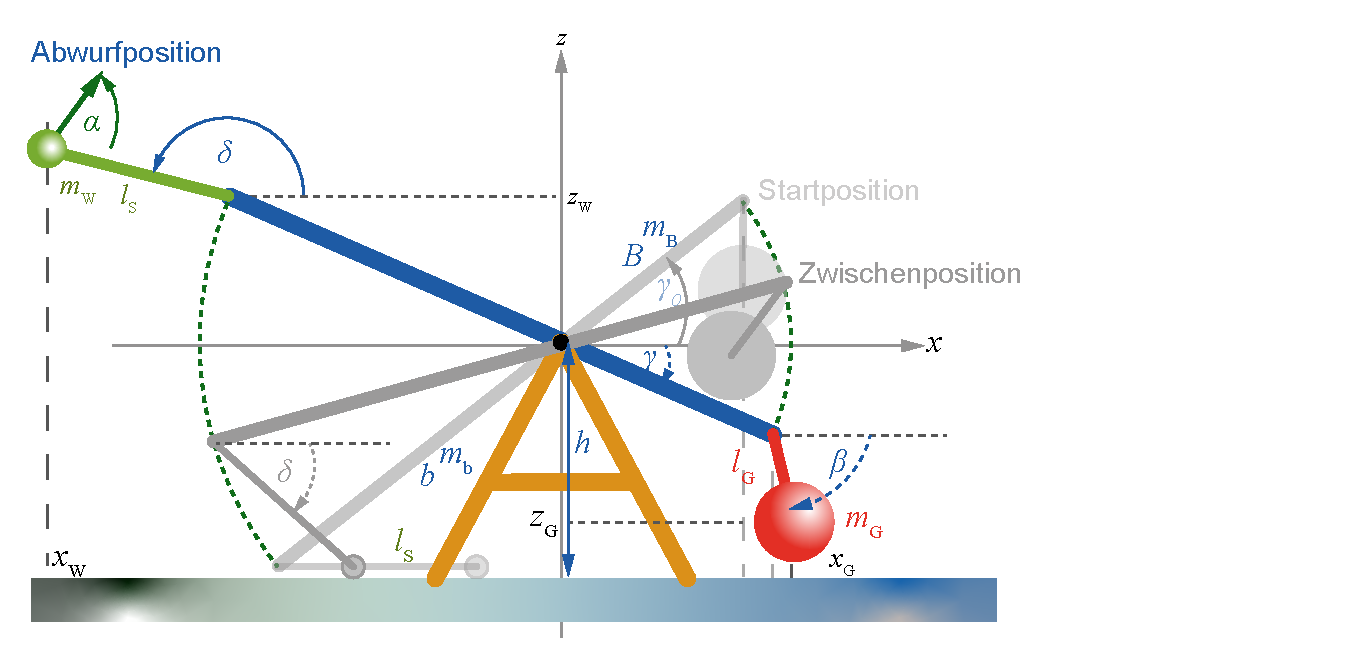
\includegraphics[width=\textwidth]{TrebNaeherung4.pdf}
\caption[Geometrie und physikalische Gr��en der Bestandteile.]{Geometrie und physikalische Gr��en der Bestandteile einer mittelalterlichen Wurfmaschine (Trebuchet, Blide).
Man beachte, dass alle Winkel au�er $\alpha$ im mathematisch positiven Drehsinn gegen die $x$-Achse als Bezugsachse definiert sind.}\label{abb:bew_TrebNaeherung4}
\end{figure}  % Negative Winkel sind im Bild als gestrichene B�gen gekennzeichnet.

Wir k�nnen nun den Wurfprozess in folgende drei Phasen unterteilen:
\begin{enumerate} [a)]
\item %a 
$0 < t \leq t_1$ Phase 1, Schleifphase\\
Das Wurfgeschoss wird beim Losl�sen der Masse $m_\text{G}$ zun�chst beschleunigt in Richtung $-\veceX$ gezogen. 
Da das Wurfgeschoss auf dem Boden aufliegt, m�ssen wir die Zwangsbedingung $z_\text{m}=-h$ beachten. 
Der Zeitpunkt $t_1$ ist dann der Moment, in dem das Wurfgeschoss gerade abhebt,
\dh zu dem die wirkende Zwangskraft Null wird.
Zu dieser Zeit entspricht die Beschleunigung des Wurfgeschosses in $z$-Richtung genau $m_\text{W} g$. 
Wir k�nnten f�r diesen Teilabschnitt ausschlie�lich mit verallgemeinerten Koordinaten $\beta$ und $\gamma$ arbeiten, indem wir die entsprechende Zwangsbedingung 
\begin{align}
	z_\text{m}=-h = - b\sin\gamma + l_\text{W}\sin\delta 
	\label{eq:bew_trebtheo01}
\end{align}
verarbeiten. 
Das f�hrt aber wegen der transzendenten Beziehungen in \eqref{eq:bew_trebtheo01}
auf sehr un�bersichtliche Bewegungsgleichungen, sodass wir auch f�r diese Phase
alle drei Winkel $\gamma$, $\delta$ und $\beta$ verwenden wollen. 
Die Zwangsbedingung ber�cksichtigen wir dann
bei der Anwendung der Methode der Lagrange-Multiplikatoren (\kap{bew_Lagrange_I}). 
Die Anfangsbedingungen sind durch $\beta_0 = \SI{-90}\degree$ und $\gamma_0$ gegeben, woraus au�erdem folgt, dass
\begin{align}
	-\delta_0 = \arcsin\lk \frac{h - b \sin\gamma_0}{l_\text{W}}\rk 
	\quad \text{und} \quad 
	h < b\,\sin\gamma_0 + l_\text{W}\,,
	\label{eq:bew_trebtheo01a}
\end{align} 
da sonst das Wurfgeschoss nicht wie gefordert auf dem Boden aufliegt.
Das Seil mit der L�nge $l_\text{W}$ wird dabei als gespannt angenommen.
\item %b 
$t_1<t<t_2$ Phase 2, Beschleunigungsphase nach oben\\
Das Wurfgeschoss hebt nun vom Boden ab ($z_\text{m}>0$), \dh es gibt nun keine Zwangsbedingungen mehr. 
Die drei Freiheitsgrade sind wieder durch die Winkel $\gamma$, $\delta$ und $\beta$ gegeben.
Die Anfangswerte sind durch die Endwerte von Phase 1 gegeben. %$\left[\beta(t_1), \gamma(t_1) ~\text{und}~ \delta(t_1)\right]$ 
\item %c
$t>t_2$ Phase 3, Flugphase\\ 
Ab $t>t_2$ bewegt sich das Geschoss frei auf der Wurfbahn des schr�gen Wurfs. 
Phase 3 wird dadurch ausgel�st, dass 
das Seil der Wurfschleuder gestoppt wird und damit das Wurfgeschoss in den schiefen Wurf (mit Luftreibung) �bergeht. 
Den entsprechenden (optimalen) Winkel zur Zeit $t_2$ bezeichnen wir mit $\gamma_2$. 
Die verallgemeinerten Koordinaten f�r diese Phase sind sinnvollerweise die kartesischen Koordinaten $x_\text{W}$ und $z_\text{m}$ mit den Bewegungsgleichungen
\begin{align}
	\ddot{x}_\text{W}+\eta \, \dot{x}_\text{W}\sqrt{\dot{x}_\text{W}{}^2+\dot{z}_\text{m}{}^2} &= \,0 \nonumber \\
	\ddot{z}_\text{m}+\eta \, \dot{z}_\text{m}\sqrt{\dot{x}_\text{W}{}^2+\dot{z}_\text{m}{}^2} \,+ \,g &= \,0 \,, \label{eq:bew_trebtheo02}
\end{align}
wobei $\eta$ der Reibungskoeffizient \[\eta= \frac{1}{2} \, c_\text{W} \, \frac{A_\text{W}} {m_\text{w}} \, \varrho_\text{L}\] ist. 
Hierin ist der Luftwiderstand $c_\text{W} \approx 0.45$, 
die Luftdichte $\varrho_\text{L}= \SI{1.3}{\kilogram\per\cubic\metre}$ 
und $A_\text{W}$ ist der Geschossquerschnitt,
der sich aus der Masse und der Dichte $\varrho_\text{W}$ des Geschosses
(bei einem Steingeschoss in etwa) $\varrho_\text{W}\approx \SI{2500}{\kilogram\per\cubic\metre}$
berechnen l�sst. 
Diese Phase soll hier nicht weiter betrachtet werden, da sie bereits ausf�hrlich in den �bungen zur Ballistik (�bungen \ref{prob:bew_Coriolis_II} bis \ref{prob:bew_Coriolis_IV}) untersucht worden ist. 
Die Anfangswerte sind durch die Endwerte von Phase 2 gegeben, n�mlich $x_\text{W}(t_2)$, $z_\text{m}(t_2)$ und 
\begin{equation}
v_\text{W} = \sqrt{\dot{x}_\text{W}(t_2)^2+\dot{z}_\text{m}(t_2)^2}\,. 
\label{eq:bew_trebtheo02a}
\end{equation}
Der Abwurfwinkel ist gegeben durch
\begin{align}
 	\alpha_\text{W} = \arctan \lk\frac{\dot{z}_\text{m}(t_2)}{\dot{x}_\text{W}(t_2)}\rk. \label{eq:bew_treb03a}
\end{align}
Mit der Zeit $t_2$ f�r die maximale Wurfweite
hat man auch $\gamma(t_2)=\gamma_2$, $\beta(t_2)$ und $\delta(t_2)$ bestimmt
und damit die Stellung des Trebuchet beim Ausl�sen des Wurfgeschosses. Zu diesem Zeitpunkt soll die Gegenmasse noch nicht den Boden erreicht haben.
\end{enumerate}
F�r die numerische Auswertung und Simulation wollen wir die in Tabelle \ref{tab:bew_trebuchet_01} angegebenen Parameter f�r das Trebuchet benutzen: \\

\begin{table}[h]
\centering
\begin{tabular}{ l C{1cm} C{1.5cm} C{1.5cm} }
\hline
  \rule{0pt}{2pt} & &  & \\
  &  & Fall A & Fall B\\
  \rule{0pt}{2pt} & &  & \\
\hline
  \rule{0pt}{9pt}%
  Balkenl�nge Gegenmasse [\si\metre] & $B$ &  4 &   3\\
  Balkenl�nge Wurfgeschoss [\si\metre] & $b$ & 12 & 15 \\
  L�nge Seil Gegenmasse  [\si\metre] & $l_\text{G}$ &  3 & 1.5 \\
  L�nge Seil Wurfgeschoss  [\si\metre] & $l_\text{S}$ &  8 & 5 \\
  H�he Balkendrehpunkt     [\si\metre] & $h$ & 10 & 10 \\
\hline
  \rule{0pt}{9pt}%
  Gegenmasse [\si\kilogram] & $m_\text{G}$ & 10000 & 15000 \\
  Masse Wurfgeschoss [\si\kilogram] & $m_\text{w}$ & 100 & 50 \\
  Masse Balken       [\si\kilogram] & $m_\text{T}$ & $\approx 1040$ & $\approx 2160$ \\
  \rule{0pt}{9pt}%
  Masse Balken pro L�nge [\si{\kilogram\per\metre}] & $\frac{\D m}{\D z}$ & $\approx 65$ & $\approx 120$ \\
  %\rule{0pt}{2pt} & &  & \\
\hline
  \rule{0pt}{9pt}%
  %Anfangswerte f�r Winkel: &  &  &  \\
  Balkenwinkel & $\gamma_0$ & $55\degree$ & $40\degree$ \\
  Pendelwinkel & $\beta_0$ & $-90\degree$ & $-90\degree$\\
  Seilwinkel der Schleuder& $\delta_0$ & $-1.2\degree$ & $-4.1\degree$\\
\hline
\end{tabular} 
\smallskip \\
\smallskip
\caption[Zwei typische Dimensionierungen einer mittelalterlichen Wurfschleuder.]{Zwei typische Dimensionierungen einer mittelalterlichen Wurfschleuder (Blide, Trebuchet).} \label{tab:bew_trebuchet_01}
\end{table}

Wie bereits an der Geometrie in \figref{bew_TrebNaeherung4} erkennbar, ist das System relativ komplex.
Wir werden uns deshalb die Dynamik des Trebuchet Schritt f�r Schritt erschlie�en.
Dabei starten wir mit einem sehr einfachen Modell und verfeinern dieses immer weiter.
Dieses Vorgehen haben wir schon mehrfach realisiert (\ua bei den verschiedenen Kreiselvarianten in \kap{bew_Lagrange_StarrerK} und \ref{kap:bew_SchwererSymmKr}) und ist immer dann zu empfehlen, um die anzuwendenden Prinzipien besser sichtbar werden zu lassen. Dar�ber hinaus erlaubt dieses Vorgehen, bei jeder Modellverfeinerung den Grenzfall des einfacheren vorherigen Modell �berpr�fen zu k�nnen.\\
Wir k�nnen die verallgemeinerten Koordinaten und Geschwindigkeiten aufschreiben, die wir zur Berechnung der Lagrange-Funktion ben�tigen. 
Diese sind f�r alle Modelle g�ltig und die entsprechenden Beziehungen k�nnen aus \figref{bew_TrebNaeherung4} abgeleitet werden.
Bei den verschiedenen behandelten N�herungen werden dann jeweils bestimmte Parameter vernachl�ssigt wie \zb $l_\text{W}$ und $l_\text{G}$. 
Wir finden f�r das Wurfgeschoss folgende Bewegungsgleichungen:
\begin{align}
	\begin{pmatrix} x_\text{W} \\ z_\text{m}  \end{pmatrix} &=
	\begin{pmatrix} -b\,\cos\gamma + l_\text{W}\,\cos\delta \\ -b\,\sin\gamma + l_\text{W}\,\sin\delta 	\end{pmatrix}, \nonumber \\
	\begin{pmatrix} \dot{x}_\text{W} \\ \dot{z}_\text{m}  \end{pmatrix} &=
	\begin{pmatrix} +b\,\dot{\gamma}\,\sin\gamma - l_\text{W}\,\dot{\delta}\,\sin\delta \\ -b\,\dot{\gamma}\,\cos\gamma + l_\text{W}\,\dot{\delta}\,\cos\delta \end{pmatrix}\,,
	\label{eq:bew_trebkoord01}
\end{align}
und f�r die Gegenmasse:
\begin{align}
	\begin{pmatrix} x_\text{G} \\ z_\text{G} 	\end{pmatrix} &=
	\begin{pmatrix} +B\,\cos\gamma + l_\text{G}\,\cos\beta \\ B\,\sin\gamma + l_\text{G}\,\sin\beta 	\end{pmatrix} \,, \nonumber \\
	\begin{pmatrix} \dot{x}_\text{G} \\ \dot{z}_\text{G} 	\end{pmatrix} &=
	\begin{pmatrix} -B\,\dot{\gamma}\,\sin\gamma - l_\text{G}\,\dot{\beta}\,\sin\beta \\ +B\,\dot{\gamma}\,\cos\gamma + l_\text{G}\,\dot{\beta}\,\cos\beta \end{pmatrix}\,.
	\label{eq:bew_trebkoord02}
\end{align}
Damit lassen sich die Lagrange-Funktionen und die Lagrange-Gleichungen in den drei generalisierten Koordinaten aufschreiben. 
Wer sich etwas Schreibarbeit sparen m�chte, nutzt dazu die Symbolic Math Toolbox (siehe \mscr{} \mlbewref{TrebSimulation.m}).\\
F�r die Lagrange-Funktion werden die kinetischen und potentiellen Energien der drei K�rper (Balken, Gegenmasse und Wurfgeschoss) addiert, also
\begin{align}
	\mathcal{L} &= T_\text{B} + T_\text{G} + T_\text{W} - f_\text{B} - f_\text{G} -f_\text{W} \,.\label{eq:bew_trebG00}
\end{align}
F�r den Balken gilt
\begin{align}
	  T_\text{B} &=  \frac{J_B}{2} \dot{\gamma}^2 \; , \nonumber \\
	  f_\text{B} &=  -\frac{1}{2}\,m_\text{T}\,g\,(b-B)\,\sin\gamma \;, \label{eq:bew_trebG01}
\end{align}
worin $J_\text{B} = \frac{1}{3}\,m_\text{T}\,\lk \frac{B^3+b^3}{B+b} \rk$ das Tr�gheitsmoment%
\footnote{Der Begriff Tr�gheitsmoment wurde genauer in \kapitel{bew_StarrerK_kin_Energie} eingef�hrt.
Hier gen�gt es, das Tr�gheitsmoment als die Summe aller Produkte der bewegten Massen mit den jeweiligen Quadraten der Abst�nde zur Drehachse zu definieren.}
eines homogenen Balkens mit der Gesamtmasse $m_\text{T} = m_\text{B}+m_\text{b}$ ist. 
F�r die Gegenmasse gilt
\begin{align}
	  T_\text{G} &=  \frac{m_\text{G}}{2} \lek B^2\,\dot{\gamma}^2 + 2 l_\text{G}\,B\,\dot{\gamma}\,\dot{\beta}\,\cos\lk\gamma-\beta\rk + l_\text{G}{}^2\,\dot{\beta}^2\rek \; , \nonumber \\
	  f_\text{G} &=  m_\text{G}\,g\, \lek  B\,\sin\gamma + l_\text{G}\,\sin\beta \rek
	  \label{eq:bew_trebG02}
\end{align}
und analog f�r das Wurfgeschoss
\begin{align}
	  T_\text{W} &=  \frac{m_\text{W}}{2} \lek b^2\,\dot{\gamma}^2 - 2 l_\text{W}\,b\,\dot{\gamma}\,\dot{\delta}\,\cos\lk\gamma-\delta\rk + l_\text{W}{}^2\,\dot{\delta}^2\rek \; , \nonumber \\
	  f_\text{W} &=  m_\text{W}\,g\, \lek -b\,\sin\gamma + l_\text{W}\,\sin\delta \rek \,. \label{eq:bew_trebG03}
\end{align}
Diese Terme k�nnen wir nun in \eqref{eq:bew_trebG00} einsetzen und erhalten nach etwas Algebra und Benutzung der Additionstheoreme f�r Winkelfunktionen
\begin{align}
	 \mathcal{L}  &= T_\text{treb} - f_\text{treb}  \nonumber \\
	 \text{mit} \quad 
	 T_\text{treb} &= \frac{J_0}{2}\,\dot{\gamma}^2\, + \frac{J_\text{G}}{2}\,\dot{\beta}^2 + \frac{J_\text{W}}{2}\,\dot{\delta}^2 + \ldots\nonumber \\
	              &~+ J_\text{BG}\,\dot{\gamma}\,\dot{\beta}\,\cos\lk\gamma-\beta\rk - J_\text{bW}\,\dot{\gamma}\,\dot{\delta}\,\cos\lk\gamma-\delta\rk\,,\nonumber \\
	f_\text{treb} &= f_0\,\sin\gamma + m_\text{G}\,l_\text{G}\,g\,\sin\beta + m_\text{w}\,l_\text{W}\,g\,\sin\delta\,. \label{eq:bew_trebG04}
\end{align}
Hier haben wir zur Abk�rzung eingef�hrt:
\begin{align}
 f_0 &= g \lek m_\text{G}\,B - m_\text{w}\,b - \frac{1}{2}m_\text{T}\lk b-B\rk \rek \nonumber \\
 J_0 &= m_\text{W}\,b^2 + m_\text{G}\,B^2+J_\text{B} \nonumber \\
 J_\text{G} &= m_\text{G}\,l_\text{G}{}^2 \nonumber \\
 J_\text{W} &= m_\text{W}\,l_\text{W}{}^2 \nonumber \\
 J_\text{BG} &= m_\text{G}\,B\,l_\text{G} \nonumber \\
 J_\text{bW} &= m_\text{W}\,b\,l_\text{W}\,. \label{eq:bew_trebG04a}
\end{align}
Die $J_i$ und $f_0$ sind Konstanten, die allein durch die Geometrie und die Massen des Trebuchet bestimmt sind.
Der Vorteil dieser Notation ist, dass mit $J_0$ und $f_0$ Grundelemente gegeben sind, die in der Lagrange-Funktion der komplexeren Trebuchet-Designs erhalten bleiben und durch Zusatzterme erweitert werden. \\

\subsubsection{Trebuchet als Wippe (Modell 1)}

\begin{figure}
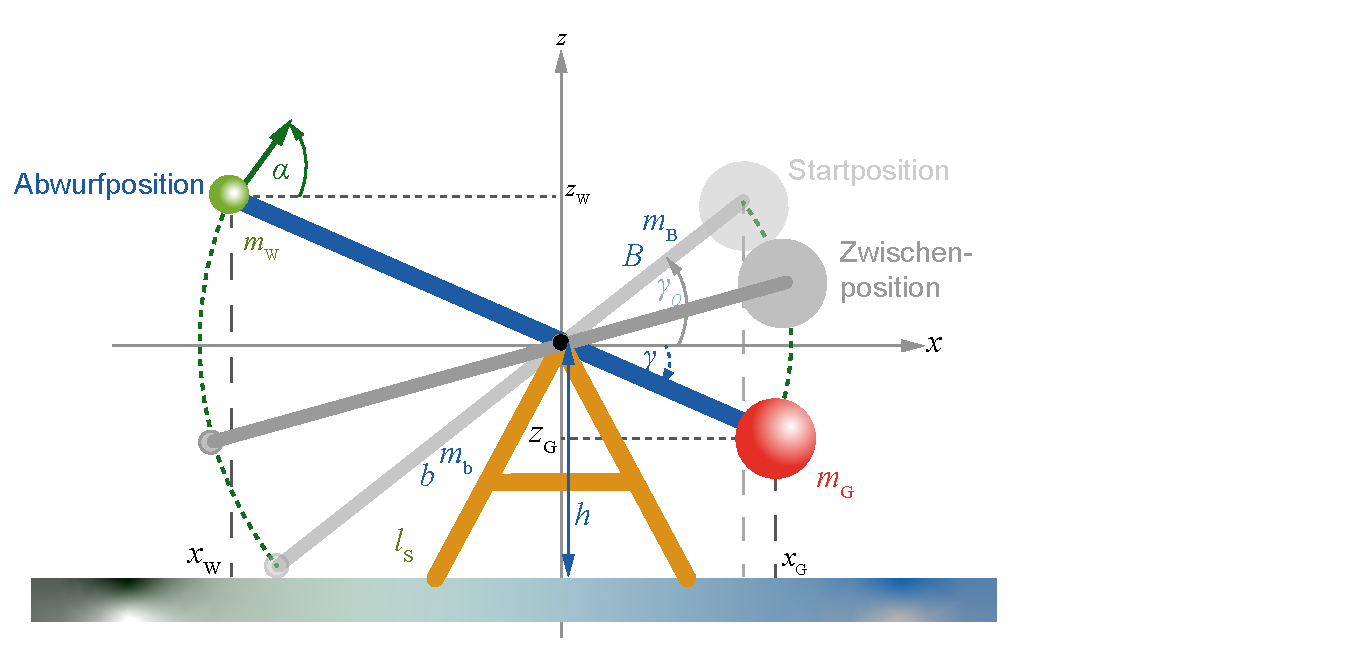
\includegraphics[width=\textwidth]{TrebNaeherung1.pdf}
\caption[Trebuchet als Wippe.]{Trebuchet als Wippe (Modell 1).}\label{abb:bew_TrebNaeherung1}
\end{figure}

Wir beginnen mit dem einfachsten Modell des Trebuchet als Wippe (\figref{bew_TrebNaeherung1}), also der Urform einer Steinschleuder, wie sie schon in der Antike bekannt war. 
Bei diesem System ist $l_\text{W} = 0$ und $l_\text{G}=0$. 
Wir haben also f�r dieses einfache Modell als generalisierte Koordinate nur den Winkel $\gamma$. 
Die Lagrange-Funktion ist dann gegeben durch
\begin{align}
		\mathcal{L}_{\uproman{1}} &= \frac{J_0}{2}\,\dot{\gamma}^2\, - \,f_0\sin\gamma \,. \label{eq:bew_treb01}
\end{align}
Da keine Zwangsbedingungen vorliegen, gibt es keine Phase 1. 
F�r Phase 2 l�sst sich folgende Bewegungsgleichung aus der Lagrange-Gleichung ableiten:
\begin{align}
		\frac{\D}{\D t}\frac{\d\mathcal{L}_{\uproman{1}}}{\d\dot{\gamma}}-\frac{\d\mathcal{L}_{\uproman{1}}}{\d\gamma} = 0 = J_0\,\ddot{\gamma} + f_0\,\cos\gamma \,. \label{eq:bew_treb02}
	\end{align}
Wie bereits erw�hnt wird Phase 3 dadurch ausgel�st, dass bei einem bestimmten (optimalen) Winkel $\gamma_2$ zur Zeit $t_2$ die Verbindung von Geschoss und Trebuchet (Schleudersack) gel�st wird und damit das Wurfgeschoss in den schr�gen Wurf �bergeht.
Wir wollen annehmen, dass dies bei demjenigen Winkel $\gamma_2$ erfolgt, f�r den die Wurfweite maximal ist.
Da beim schr�gen Wurf die Wurfweite sowohl von der Anfangsgeschwindigkeit als auch dem Abwurfwinkel abh�ngt, muss man also f�r verschiedene $t_2$ den Winkel $\alpha_\text{W}$ und die Geschwindigkeit 
$v_\text{W}$ \eqref{eq:bew_trebtheo02a} aus den Bewegungsgleichungen \eqref{eq:bew_trebtheo02} berechnen und daraus die erzielbare Wurfweite $W$ bestimmen.
Wir k�nnen das numerisch tun oder aber unsere analytischen Betrachtungen nutzen.
F�r vernachl�ssigbare Reibung lautet die Gleichung f�r die Reichweite bei einem schiefen Wurf mit einer Anfangsh�he $z_\text{W}(t_2) = z_\text{W2}$ und einem Abwurfwinkel $\alpha_\text{W}$
		\begin{align}
				W = \frac{v_2}{g} \cos\alpha_\text{W} \lk v_2\,\sin\alpha_\text{W} + \sqrt{{v}_2{}^2 \,(\sin\alpha_\text{W})^2 + 2\,g\,z_\text{W2}}\rk \,. \label{eq:bew_treb03}
		\end{align}
Mit dem so bestimmten $\alpha_\text{W}$ f�r die maximale Wurfweite findet man die Stellung des Trebuchet beim Ausl�sen des Wurfgeschosses.
Die entsprechende Dynamik ist in \figref{bew_TrebErgebnis1b} gezeigt (siehe \mscr{} \mlbewref{TrebSimulation.m}).
Wie man erkennt, ist die Energieumwandlung bei diesem System nicht optimal, ein erheblicher Teil der potentiellen Energie der Gegenmasse geht in kinetische Energie derselben �ber (vor allem durch einen Impuls in $x$-Richtung).
Man erzielt mit diesem System nur Reichweiten geringer als $\SI{100}{\metre}$.
Au�erdem wird ersichtlich, dass die Reichweite relativ kritisch vom Ausl�sezeitpunkt $t_2$ abh�ngt.\\

\begin{figure}
\begin{minipage}{\textwidth}
\leftfigure{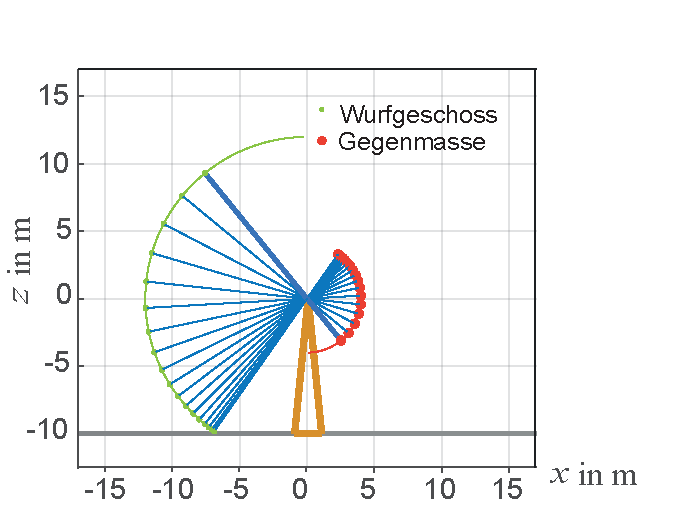
\includegraphics[width=0.5\textwidth]{TrebSim01b.pdf}}%
\hspace{\fill}
\rightfigure{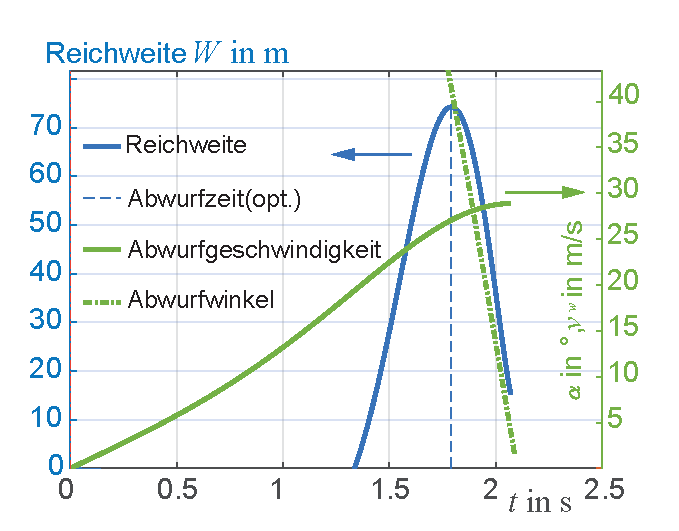
\includegraphics[width=0.5\textwidth]{TrebSim01a.pdf}}
\leftcaption[Dynamik der einfachen Steinschleuder.]{Dynamik der einfachen Steinschleuder (Modell 1).} \label{abb:bew_TrebErgebnis1b}
\rightcaption[Reichweite der einfachen Steinschleuder.]{Reichweite der einfachen Steinschleuder (Modell 1).} \label{abb:bew_TrebErgebnis1a}
\end{minipage}
\end{figure}

Wir k�nnen nun noch (und auch f�r alle folgenden Trebuchet-Modelle in gleicher Form) zwei Effizienzparameter definieren.
Die \emph{Reichweiteneffizienz}:
	\begin{align}
		\epsilon_\text{W} &= \frac{W}{W_\text{max}} \nonumber \\
		\text{mit} \quad 
		W_\text{max} &= \frac{2 \Delta U}{m_\text{W}\,g } \sqrt{\frac{z_\text{W}(t_2)}{\Delta U}\,m_\text{W}\,g+1} \nonumber \\
		\text{und} \quad 
		\Delta U &= -\lek U(t_2)-U(t_0)\rek \,.\label{eq:bew_treb04a}
	\end{align}
Dabei haben wir angenommen, dass alle \anf{freiwerdende} Energie 
vollst�ndig in kinetische Energie des Wurfgeschosses gewandelt wird.
Die Verringerung der potentiellen Energie der Gegenmasse 
abz�glich der Zunahme der potentiellen Energie von Balken und Wurfgeschoss
werden somit in einen optimalen Wurf umgesetzt.\\
Als zweiten Effizienzparameter definieren wir die 
\emph{Umwandlungseffizienz der potentiellen Energie} der Gegenmasse
\begin{align}
	\epsilon_\text{T} = \frac{T_\text{W}(t_2)}{\Delta U} \,, \label{eq:bew_treb04b}
\end{align}
worin $T_\text{W}(t_2)$ die kinetische Energie des Wurfgeschosses zum Zeitpunkt $t_2$ ist.
F�r die Werte aus Tabelle \ref{tab:bew_trebuchet_01} ergeben sich beispielhaft f�r Fall A folgende Effizienzparameter:
	\[ 
	\epsilon_\text{W} = 6.7 \% ~,~~\epsilon_\text{T} = 6.8 \% \,,
\]
was best�tigt, dass die Energieumwandlung bei diesem System suboptimal ist.

\begin{table}[h]
  \centering
  \begin{tabular}[h]{|l|c|r@.l|r@.l|r@.l|r@.l|r@.l|r|r|}
  \hline
%  \rule{0pt}{2pt}\\
  \phantom{x}&\phantom{x}&\multicolumn2{c|}{\phantom{x}}&\multicolumn2{c|}{\phantom{x}}&\multicolumn2{c|}{\phantom{x}}&\multicolumn2{c|}{\phantom{x}}&\multicolumn2{c|}{\phantom{x}}&\phantom{x}&\phantom{x}\\
  Parameter& ZB & \multicolumn2{c|}{$W$}   &  \multicolumn2{c|}{$t_\text{abw}$}    & \multicolumn2{c|}{$\alpha$}  & \multicolumn2{c|}{$v_\text{abw}$}    & \multicolumn2{c|}{$\epsilon_\text{T}$}   & $l_\text{G}$  & $l_\text{W}$  \\
  Einheit  &         &\multicolumn2{c|}{\si{\metre}} & \multicolumn2{c|}{\si{\second}} & \multicolumn2{c|}{\si{\degree}} & \multicolumn2{c|}{\si{\metre\per\second}} & \multicolumn2{c|}{\si{\%}} & q \si{\metre} & \si{\metre} \\
%  \rule{0pt}{2pt}\\
  \phantom{x}&\phantom{x}&\multicolumn2{c|}{\phantom{x}}&\multicolumn2{c|}{\phantom{x}}&\multicolumn2{c|}{\phantom{x}}&\multicolumn2{c|}{\phantom{x}}&\multicolumn2{c|}{\phantom{x}}&\phantom{x}&\phantom{x}\\
  \hline
  Modell 1 & nein    & 74&3& 1&78 & 40&4 & 27&0 &  6&8 & 0 & 0 \\
  Modell 2 & nein    &251&5& 1&60 & 29&6 & 53&4 & 23&7 & 3 & 0 \\
  Modell 3 & nein    &274&9& 1&90 & 42&3 & 51&9 & 24&1 & 0 & 8 \\
  Modell 4 & nein    &355&5& 1&66 & 37&3 & 60&0 & 28&7 & 3 & 8 \\
  Modell 4 & ja      &296&2& 1&58 & 35&1 & 55&4 & 19&6 & 3 & 8 \\
  FAT I    & nein    &432&9& 1&98 & 37&6 & 66&2 & 33&4 & 0 & 8 \\
  FAT II   & ja      &294&9& 2&18 & 36&1 & 55&0 & 29&5 & 0 & 8 \\
  \hline
  \end{tabular}
\caption[Vergleich der Reichweiten und Effizienzparameter verschiedener Trebuchet-Modelle.]{Vergleich der Reichweiten und Effizienzparameter verschiedener Trebuchet-Modelle. ZB steht f�r Zwangsbedingungen, FAT f�r \textit{Floating Arm Trebuchet}, siehe \probref{bew_Trebuchet}. Weitere Parameter: $h =\SI{10}{\metre}$, $m_\text{G} = \SI{10000}{\kilogram}$, $m_\text{W}= \SI{100}{\kilogram}$, $m_\text{T} = \SI{1040}{\kilogram}$, $B = \SI{4}{\metre}$, $b=\SI{12}{\metre}$.}
\label{tab:bew_trebuchet_02}
\end{table}


\subsubsection{Trebuchet mit pendelnder Gegenmasse (Modell 2)}

\begin{figure}
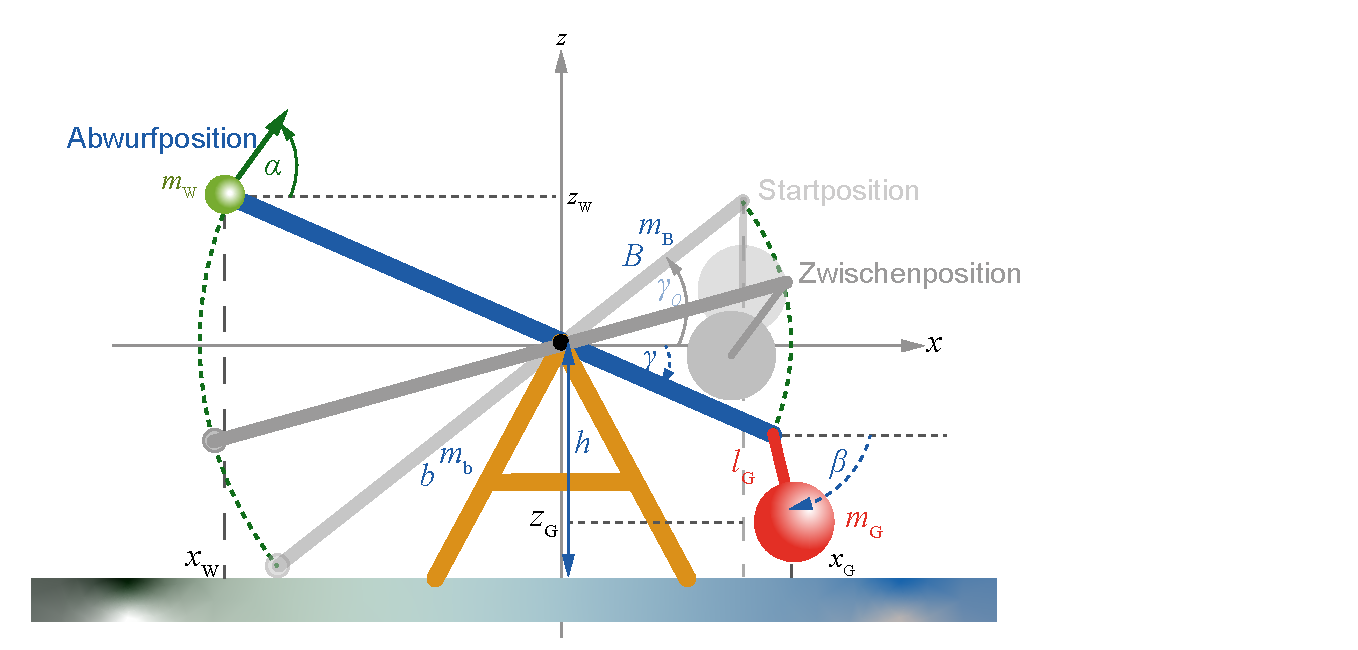
\includegraphics[width=\textwidth]{TrebNaeherung2.pdf}
\caption[Trebuchet mit pendelnder Gegenmasse.]{Trebuchet mit pendelnder Gegenmasse (Modell 2).}\label{abb:bew_TrebNaeherung2}
\end{figure}

Bei diesem Modell ist die Gegenmasse als Pendel aufgeh�ngt.
Dadurch kann die Reichweite deutlich gesteigert werden, da die Umwandlung von potentieller Energie der Gegenmasse in kinetische Energie (Impuls in $x$-Richtung) derselben durch die Pendelaufh�ngung deutlich reduziert wird. 
Die Lagrange-Funktion erweitert sich durch die neue Koordinate $\beta$ und ergibt sich nun aus \eqref{eq:bew_trebG04} zu
\begin{align}
		\mathcal{L}_{\uproman{2}} &= \mathcal{L}_{\uproman{1}} + \Delta\mathcal{L}_{\uproman{2}}  \nonumber \\
		&= \frac{J_0}{2}\,\dot{\gamma}^2 - f_0\,\sin\gamma + \ldots  \nonumber \\
		&~~+\frac{1}{2}\,J_\text{G}\,\dot{\beta}^2 + J_\text{BG}\,\dot{\gamma}\,\dot{\beta}\,\cos\lk \gamma-\beta \rk  - m_\text{G}\,l_\text{G}\,g\,\sin\beta \,. \label{eq:bew_treb05}
\end{align}
Daraus erhalten wir die Bewegungsgleichungen
\begin{align}
    \begin{split}
        J_0\,\ddot{\gamma}        &= -J_\text{BG}\,\ddot{\beta}\,\cos\lk \beta-\gamma\rk  + J_\text{BG}\,\dot{\beta}^2\,\sin\lk \beta-\gamma \rk - f_0\,\cos\gamma \,, \\
        J_\text{G}\,\ddot{\beta}  &= -J_\text{BG}\,\ddot{\gamma}\,\cos\lk \beta-\gamma\rk - J_\text{BG}\,\dot{\gamma}^2\,\sin\lk \beta-\gamma\rk - g\,m_\text{G}\,l_\text{G}\,\cos\beta \,. \label{eq:bew_treb06}
    \end{split}
\end{align}
Wir wollen dieses Differentialgleichungssystem wieder numerisch in \matlab{} integrieren.
Wir erkennen, dass man \eqref{eq:bew_treb06} in Matrixform schreiben kann.
Wir bringen dazu die Terme mit den zweiten Ableitungen auf die linke Seite und schreiben
\begin{align}
		\mathbb{M}(t,\vec{q}) \cdot \ddot{\vec{q}}  
			& = 
\begin{pmatrix}
J_0  & J_\text{BG}\,\cos\lk \beta-\gamma \rk \\
J_\text{BG}\,\cos\lk \beta-\gamma \rk & J_\text{G}
\end{pmatrix}
\begin{bmatrix}
		\ddot{\gamma} \\
		\ddot{\beta} 
\end{bmatrix} \nonumber \\
		&=
\begin{pmatrix}
+J_\text{BG}\,\dot{\beta}^2\,\sin\lk \beta-\gamma \rk - f_0\,\cos\gamma \\
-J_\text{BG}\,\dot{\gamma}^2\,\sin\lk \beta-\gamma \rk - g\,m_\text{G}\,l_\text{G}\,\cos\beta
\end{pmatrix}
\nonumber \\
&= \vec{F}(t,\vec{q},\dot{\vec{q}}) \, \label{eq:bew_treb07}
\end{align}
mit $\vec{q} =[\gamma,\beta]^\text{T}$, $\dot{\vec{q}} =[\dot{\gamma},\dot{\beta}]^\text{T}$ und $\ddot{\vec{q}} =[\ddot{\gamma},\ddot{\beta}]^\text{T}$. 
Der Vektor $\vec{F}(t,\vec{q},\dot{\vec{q}})$ hat die Dimension einer Kraft \bzw hier eines Drehmomentes. 
Die Elemente der Matrix auf der linken Seite sind Tr�gheitsmomente \bzw Massen, deshalb nennt man sie auch Massen- oder Tr�gheitsmoment-Matrix\index{Tr�gheitsmoment-Matrix}. 
F�r die numerische L�sung m�ssen wir diese aber noch etwas aufbereiten, da \matlab{} ja eine Routine zur Integration von Differentialgleichungssystemen erster Ordnung der Form $\dot{\vec{Y}} = \vec{f}_\text{g}(t, \vec{Y})$ zur Verf�gung stellt, in der die $Y_i(t)$ die gesuchten Funktionen sind. 
Wir setzen deshalb:
		\begin{align*} 
				\left[Y_1, Y_2,~ Y_3,~Y_4 \right]^\text{T} = \left[\gamma,~\dot{\gamma},~\beta,~\dot{\beta} \right]^\text{T} \,
		\end{align*}
und m�ssen dann auch die Massen-Matrix durch entsprechende Zeilen und Spalten erweitern.
Wir wollen diese auch weiterhin Massen-Matrix \cite{Wells1967, MATLABEx01}\index{Massen-Matrix} nennen.
Das DGL-System kann schlie�lich in folgender nun \matlab-kompatibler Form geschrieben werden:
\begin{align}
    \mathbb{M}(t,\vec{Y}) \cdot \dot{\vec{Y}}  &= 
    \begin{pmatrix}
	1 \quad\quad & 0  & 0 \quad\quad  & 0  \\
	0 & J_0 & 0    & J_\text{BG}\,\cos \lk Y_3-Y_1 \rk \\
	0 & 0 & 1    & 0  \\
	0 & J_\text{BG}\,\cos(Y_3-Y_1) & 0    & J_\text{G}
    \end{pmatrix} \cdot
    \begin{bmatrix}
	\dot{Y}_1 \\
	\dot{Y}_2 \\
	\dot{Y}_3 \\
	\dot{Y}_4 
    \end{bmatrix} \nonumber \\
    &= \begin{pmatrix}
	Y_2 \\
	J_\text{BG}\,Y_4^2\,\sin\lk Y_3-Y_1 \rk - f_0\,\cos Y_1\\
	Y_4 \\
	-J_\text{BG}\,Y_2^2\,\sin\lk Y_3-Y_1 \rk - g\,m_\text{G}\,l_\text{G}\,\cos Y_3 
    \end{pmatrix} \nonumber \\
    &= \vec{F}(t,\vec{Y},\dot{\vec{Y}}) \,. \label{eq:bew_treb08}
\end{align} 
Die Berechnung der L�sung des DGL-Systems mittels \matlab{} erfolgt gem�� der \kap{bew_matlab_dgl} beschriebenen Vorgehensweise zur L�sung von Gleichungssystemen der  Form $\D\vec{Y}/\D t = \vec{F}(t,\vec{Y},\dot{\vec{Y}})$. Hier wird beim Aufruf der \matlab{} Routine \odevf{} eine (gegebenenfalls parametrisierte) Matrix-Funktion $\mathbb{M} = \mathbb{M}(t,\vec{Y},P)$ �bergeben. Dabei ist $P$ ist eine vorteilhafte Struktur f�r den Parametersatz, in unserem Fall im Wesentlichen bestehend aus den geometrischen und physikalischen Parametern des Trebuchet.\\

\begin{figure}
\begin{minipage}{\textwidth}
\leftfigure{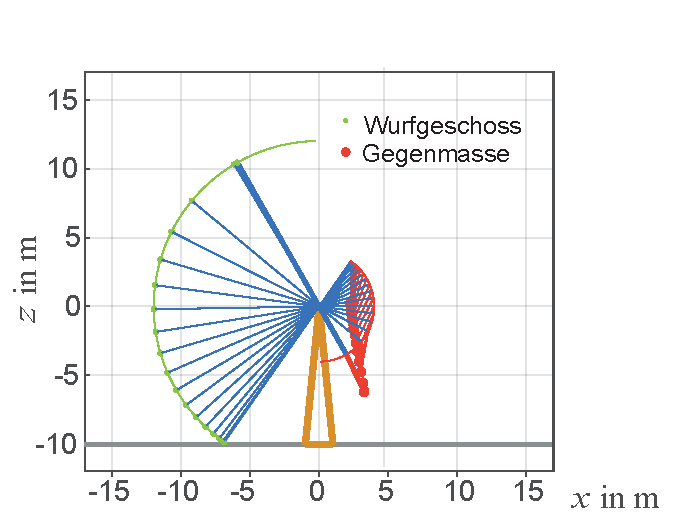
\includegraphics[width=0.5\textwidth]{TrebSim02b.pdf}}%
\hspace{\fill}
\rightfigure{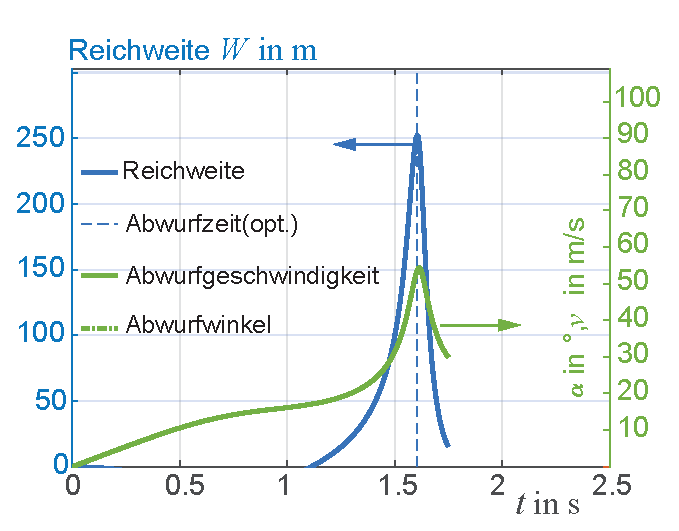
\includegraphics[width=0.5\textwidth]{TrebSim02a.pdf}}
\leftcaption[Dynamik eines Trebuchet mit pendelnder Gegenmasse.]{Dynamik eines Trebuchet mit pendelnder Gegenmasse (Modell 2).} \label{abb:bew_TrebErgebnis2a}
\rightcaption[Reichweite eines Trebuchet mit pendelnder Gegenmasse.]{Reichweite eines Trebuchet mit pendelnder Gegenmasse (Modell 2).} \label{abb:bew_TrebErgebnis2b}
\end{minipage}
\end{figure}

Die Rechnungen sind im Detail im  \mscr{} \mlbewref{TrebSimulation.m} ausgef�hrt,
die wesentlichen Ergebnisse sind in den \figref{bew_TrebErgebnis2a}
und \figref{bew_TrebErgebnis2b}, sowie in Tabelle \ref{tab:bew_trebuchet_02} gezeigt.
Wie erwartet, ist die Energieumwandlung bei diesem System deutlich besser
und damit auch bei sonst gleichen Parametern die erzielbaren Reichweiten. 
Diese liegen �ber $\SI{250}{\metre}$,
das bedeutet also fast eine Steigerung um den Faktor drei bis f�nf. 
Die Erkl�rung wird noch einmal durch die Dynamik in \figref{bew_TrebErgebnis2b} verdeutlicht. 
Die Gegenmasse wird durch die Pendelaufh�ngung aufgrund der Tr�gheit
kaum in $x$-Richtung beschleunigt, sondern bewegt sich nahezu vertikal nach unten. 
Zum Zeitpunkt des Abwurfs $t_2$ zeigt dazu die Pendelachse
ann�hernd in die Richtung des momentanen Balkenwinkels $\gamma$,
was die Energieumwandlungseffizienz nochmals verbessert.%
\footnote{Man kann das Pendeln der Gegenmasse auch als parametrische Schaukel verstehen.}
Aus \figref{bew_TrebErgebnis2a} wird aber auch ersichtlich, wie eng der Ausl�sebereich
f�r den weitesten Wurf \bzw die gew�nschte Reichweite ist.
Das stellte offensichtlich erhebliche Anforderungen an die Konstruktion der Ausl�semechanik.



\subsubsection{Trebuchet mit Schleuder aber fester Gegenmasse (Modell 3)}

\begin{figure}
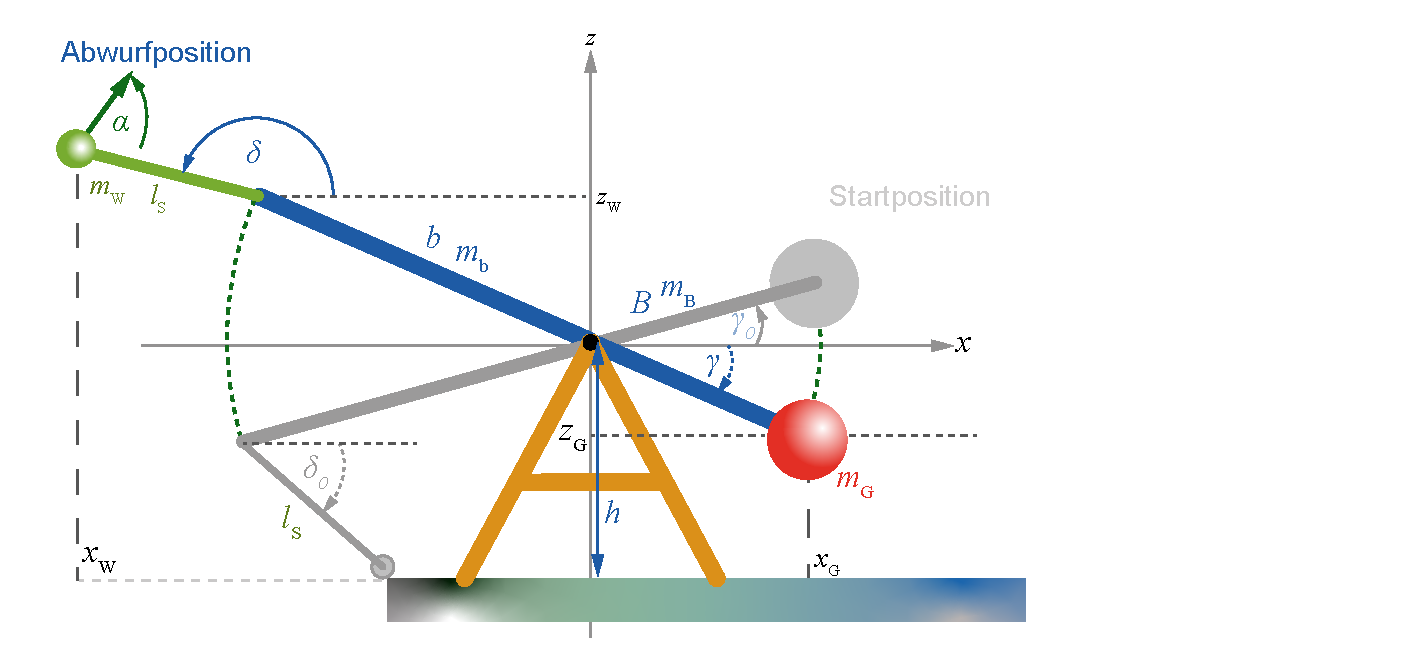
\includegraphics[width=\textwidth]{TrebNaeherung3.pdf}
\caption[Trebuchet mit Schleuder und fester Gegenmasse.]{Trebuchet mit Schleuder und fester Gegenmasse (Modell 3).}\label{abb:bew_TrebNaeherung3}
\end{figure}

Hier nehmen wir nun an, dass sich das Wurfgeschoss in einer Schleuder der L�nge $l_\text{W}$ befindet (\figref{bew_TrebNaeherung3}).
Dabei wird zugelassen, dass das Wurfgeschoss in seiner Beschleunigungsphase tiefer gelangen kann als es zum Zeitpunkt des Starts der Schleuder lag, wozu man im Mittelalter entsprechende Gr�ben aushub. 
Mit dieser Annahme unterliegt die Bewegung der Schleuder weiterhin keinen Zwangsbedingungen.
Als neue generalisierte Koordinate haben wir den Winkel $\delta$, der zum Startzeitpunkt so gew�hlt werden soll, dass die Schleuder gestrafft auf dem Boden liegt, \dh \[-\delta_0 = \arcsin\lk \frac{h-b\,\sin\gamma_0}{l_\text{W}}\rk\,. \]
Die Lagrange-Funktion f�r diesen Fall lautet 
	\begin{align}
		\mathcal{L}_{\uproman{3}} &= \mathcal{L}_{\uproman{1}} + \Delta\mathcal{L}_{\uproman{3}}  \nonumber \\
			& = \frac{J_0}{2}\,\dot{\gamma}^2 - f_0\,\sin\gamma + \ldots  \nonumber \\
			& ~~+ \frac{1}{2} J_\text{W}\,{\dot{\delta}}^2-J_\text{bW}\,\dot{\gamma}\,\dot{\delta}\,\cos\lk \gamma-\delta\rk - g\,m_\text{W}\,l_\text{W}\,\sin\delta\,, \label{eq:bew_treb09}
	\end{align}
woraus die Bewegungsgleichungen in Matrixform 
\begin{align}
		\mathbb{M}(t,\vec{q}) \cdot \ddot{\vec{q}}  
			& = 
\begin{pmatrix}
	J_0  ~~ & -J_\text{bW}\,\cos\lk \delta-\gamma \rk \\
			  -J_\text{bW}\,\cos\lk \delta-\gamma \rk ~~& J_\text{W}
\end{pmatrix}
\begin{bmatrix}
	\ddot{\gamma} \\
	\ddot{\delta} 
\end{bmatrix} \nonumber \\
	&= \begin{pmatrix}
	 -J_\text{bW}\,\dot{\beta}^2\,\sin\lk \beta-\gamma \rk - f_0\,\cos\gamma \\
	 +J_\text{bW}\,\dot{\gamma}^2\,\sin\lk \beta-\gamma \rk - g\,m_\text{W}\,l_\text{W}\,\cos\beta
\end{pmatrix} \nonumber \\
&= \vec{F}(t,\vec{q},\dot{\vec{q}}) \, \label{eq:bew_treb10}
\end{align}
folgen.
Auch hier integrieren wir die Bewegungsgleichungen numerisch
wie im vorherigen Abschnitt beschrieben und erkennen in
\figref{bew_TrebErgebnis3a} und Tabelle \ref{tab:bew_trebuchet_02}
ebenfalls eine deutliche Steigerung der Reichweite
und der Energieeffizienz gegen�ber der einfachen Steinschleuder. 
Diese resultieren aus der effektiven Verl�ngerung des Wurfarms durch die Schleuder, welche wiederum zu einer h�heren Abwurfgeschwindigkeit f�hrt.
Wir erkennen au�erdem, dass die maximale Reichweite weniger stark vom Ausl�sezeitpunkt abh�ngt.
Das bringt uns auf die Idee, die Modelle 2 und 3 zu kombinieren.

\begin{figure}
\begin{minipage}{\textwidth}
\leftfigure{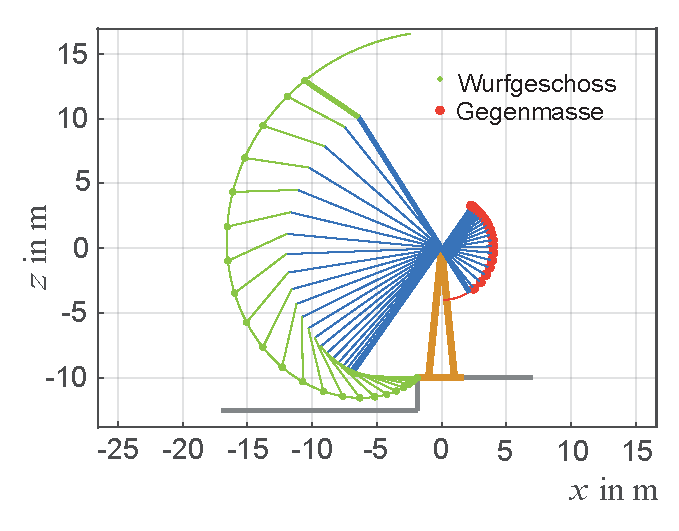
\includegraphics[width=0.5\textwidth]{TrebSim03b.pdf}}%
\hspace{\fill}
\rightfigure{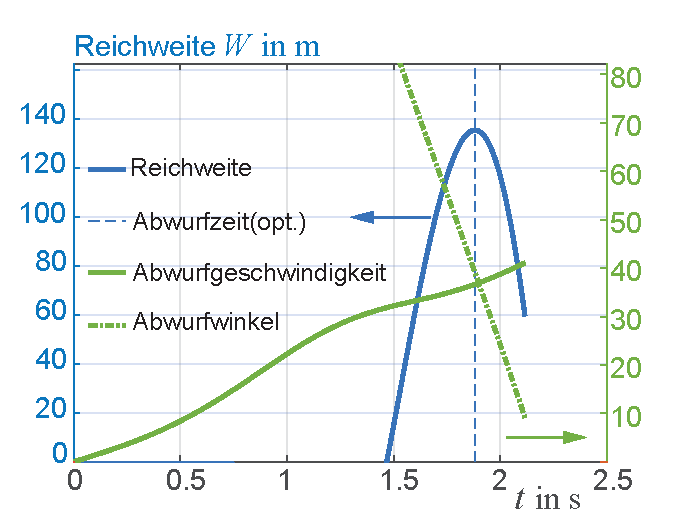
\includegraphics[width=0.5\textwidth]{TrebSim03a.pdf}}
\leftcaption[Dynamik eines Trebuchet mit Schleuder und fester Gegenmasse.]{Dynamik eines Trebuchet mit Schleuder und fester Gegenmasse (Modell 3).} \label{abb:bew_TrebErgebnis3b}
\rightcaption[Reichweite eines Trebuchet mit Schleuder und fester Gegenmasse.]{Reichweite eines Trebuchet mit Schleuder und fester Gegenmasse (Modell 3).} \label{abb:bew_TrebErgebnis3a}
\end{minipage}
\end{figure}

\subsubsection{Vollst�ndiges Trebuchet (Modell 4)} \label{kap:bew_trebuchet_complete}

Wir bringen nun alle Bauvarianten zusammen (\figref{bew_TrebNaeherung4}). 
Jetzt wollen wir auch ber�cksichtigen, dass zu Beginn der Bewegung die Schleuder mit dem Wurfgeschoss einer Zwangsbedingung unterliegt,
da sich das Wurfgeschoss in der Schleuder in der H�he $z_\text{W} = -h$ auf dem Boden bewegt, \dh es gilt die Zwangsbedingung \eqref{eq:bew_trebtheo01}:
		\begin{align}
				f\lk \gamma, \delta\rk = h -  b\,\sin\gamma + l_\text{W}\,\sin\delta = 0 \,. \label{eq:bew_treb11}
		\end{align}
Mit der Methode der Lagrange-Multiplikatoren (\kap{bew_Lagrange_I}) schreiben wir die Lagrange-Funktion als
		\begin{align}
		\begin{split}
				\mathcal{L}_{\uproman{4}} &=  \mathcal{L}_{\uproman{1}} + \Delta\mathcal{L}_{\uproman{2}} + \Delta\mathcal{L}_{\uproman{3}} + \ldots \\ 
				& ~~+ \frac{1}{2}J_0\,\dot{\gamma}^2 - f_0\,\sin\gamma  + \ldots \\
				& ~~+ \frac{1}{2}J_\text{G}{}^2\,\dot{\beta}^2 + J_\text{BG}\,\dot{\gamma}\,\dot{\beta}\,\cos\lk\gamma-\beta\rk - g\,m_\text{G}\,l_\text{G}\,\sin\beta
				+ \ldots \\
				& ~~+ \frac{1}{2}\,J_\text{W}\,\dot{\delta}^2 - J_\text{bW}\,\dot{\gamma}\,\dot{\delta}\,\cos\lk\gamma-\delta\rk - g\,m_\text{W}\,l_\text{W}\,\sin\delta + \ldots\\
				& ~~ + \lambda\lk h -  b\,\sin\gamma + l_\text{W}\,\sin\delta \rk \,.  \label{eq:bew_treb12}
		\end{split}
		\end{align}
Die Zwangskraft $\lambda$ h�lt das Wurfgeschoss auf der Bodenebene, sie ist $-m\,g$ beim Start des Trebuchet und wird Null beim \anf{Abheben}.
Zu diesem Zeitpunkt verliert auch die Zwangsbedingung ihre G�ltigkeit. 
Man muss also bei der numerischen Rechnung immer �berpr�fen, ob die Zwangsbedingung noch gilt.
Ebenso m�ssen die Anfangsbedingungen die Zwangsbedingung erf�llen.\\
Damit ergeben sich f�r $\gamma, \beta$, $\delta$ und $\lambda$ die folgenden drei Bewegungsgleichungen:
\begin{align}
	J_0\,\ddot{\gamma} 
		&= - m_\text{G}\,B\,l_\text{G}\,\ddot{\beta}\,\sin\lk \gamma+\beta\rk + m_\text{W}\,b\,l_\text{W}\,\ddot{\delta}\,\cos\lk\delta-\gamma\rk + \ldots  \nonumber \\
		&\quad + m_\text{G}\,B\,l_\text{G}\,\dot{\beta}^2\,\sin\lk\beta - \gamma\rk -m_\text{W}\,b\,l_\text{W}\,\dot{\delta}^2\,\sin\lk\delta-\gamma\rk - \ldots \nonumber  \\
		&\quad - f_0 \cos\gamma - \lambda\,b\,\cos\gamma \,, \\ \label{eq:bew_treb13}
	J_\text{G}\,\ddot{\beta}  &= -J_\text{BG}\,\ddot{\gamma}\cos\lk\beta-\gamma\rk - J_\text{BG}\dot{\gamma}^2\,\sin\lk\beta-\gamma\rk-g\,m_\text{G}\,l_\text{G}\,\cos\beta \,, \nonumber \\
	J_\text{W}\,\ddot{\delta} &= +J_\text{bW}\,\ddot{\gamma}\cos\lk\delta-\gamma\rk +J_\text{bW}\dot{\gamma}^2\,\sin\lk\delta-\gamma\rk-g\,m_\text{W}\,l_\text{W}\,l_\text{W}\,\cos\delta + \ldots \nonumber \\
		&\quad + \lambda\,\cos\delta \,.
\end{align}
Ferner ist die Zwangsbedingung \eqref{eq:bew_treb11} zu ber�cksichtigen. Wir k�nnten nun entsprechend der L�sungs--hinweise in \kapitel{bew_Lagrange_I} vorgehen.
Die analytische Berechnung wird aufgrund der Winkelfunktionsterme relativ un�bersichtlich und komplex, l�sst sich aber ohne weiteres in \matlab{} behandeln.
Wir wollen hier einen anderen Weg gehen, der sich an der Matrixstruktur der Bewegungsgleichungen \eqref{eq:bew_treb08} orientiert und daher besonders f�r die numerische Behandlung in \matlab{} geeignet ist.
Diese Methode l�sst sich verallgemeinern und kann insbesondere auch verwendet werden, wenn mehrere komplexe Zwangsbedingungen vorliegen und der oben beschriebene Ansatz an seine Grenzen kommt. 

Wir schreiben die Bewegungsgleichungen \eqref{eq:bew_treb13} wieder in Matrixform:
\begin{align}
			\mathbb{M}(\vec{q}) \cdot \ddot{\vec{q}} + \lambda \frac{\d f}{\d \vec{q}} = \vec{F}(\vec{q},\dot{\vec{q}})\,. \label{eq:bew_treb14}
\end{align}
Hierin ist
\begin{align}
\begin{split}
  \frac{\d f}{\d \vec{q}} &= \left[-b\,\cos\gamma~, ~0~,~l_\text{W}\,\cos\delta \right] \,,~~\vec{q} =[\gamma,\beta,\delta]^\text{T} \,,~~\\
	\dot{\vec{q}} &=[\dot\gamma,\dot\beta,\dot\delta]^\text{T} \,~~\text{und}~~\ddot{\vec{q}} =[\ddot{\gamma},~\ddot{\beta},~\ddot{\delta}]^\text{T} \,. 
\end{split} \label{eq:bew_treb14a}
\end{align}
Es sei betont, dass die Massen-Matrix $\mathbb{M}$ und der Kraftvektor $\vec{F}$ f�r das System ohne Zwangsbedingung aufgeschrieben wurden. 
\begin{align}
		\begin{split}
		\mathbb{M} = 
\begin{pmatrix}
	+J_0 & +J_\text{BG}\,\cos\lk\gamma-\beta\rk  & -J_\text{bW}\,\cos\lk\gamma-\delta\rk \\ \label{eq:bew_treb14b}
	+J_\text{BG}\,\cos\lk\gamma-\beta\rk   & +J_\text{G}  & 0\\
	-J_\text{bW}\,\cos\lk\gamma-\delta\rk   & 0   & +J_\text{W}
\end{pmatrix}\,.
\end{split}
\end{align}
Der Kraftvektor $\vec{F}$ ist gegeben durch
\begin{align}
\begin{split}
		\vec{F} = 
\begin{pmatrix}
	-J_\text{BG}\,{\dot{\beta}}^2\sin\lk\gamma-\beta\rk + J_\text{bW}\,{\dot{\delta}}^2\sin\lk\gamma-\delta\rk - f_0\,\cos\gamma \\
	+J_\text{BG}\,{\dot{\gamma}}^2\sin\lk\gamma-\beta\rk - m_\text{G}\,l_\text{G}\,g\,\cos\beta \\ \label{eq:bew_treb14c}
	-J_\text{bW}\,{\dot{\delta}}^2\sin\lk\gamma-\delta\rk - m_\text{W}\,l_\text{W}\,g\,\cos\delta
\end{pmatrix}\,.
\end{split}
\end{align}
Da die Zwangsbedingung in unserem Fall nicht explizit von der Zeit abh�ngt, gilt
\begin{align*}
		\frac{\D f}{\D t} = 0 = \frac{\d f}{\d \vec{q}} \cdot \dot{\vec{q}} \,, 
\end{align*}
woraus f�r die zweite Ableitung sofort folgt:
\begin{align}
		\frac{\D^2 f}{\D\,t^2} &= 0 = \frac{\d }{\d \vec{q}} \lk \frac{\d f}{\d \vec{q}} \cdot \dot{\vec{q}} \rk \cdot \dot{\vec{q}} + \frac{\d f}{\d \vec{q}} \cdot \ddot{\vec{q}} \quad
		\rightarrow \quad \frac{\d f}{\d \vec{q}} \cdot \ddot{\vec{q}} = -\frac{\d }{\d \vec{q}} \lk \frac{\d f}{\d \vec{q}} \cdot \dot{\vec{q}} \rk \cdot \dot{\vec{q}} = F_{\lambda} \,. \label{eq:bew_treb15}
\end{align}
In unserem Fall%
\footnote{$F_\lambda$ ist, wenn wir die Zwangsbedingung in der Dimension L�nge aufschreiben,
unabh�ngig von der Wahl der generalisierten Koordinaten eine Beschleunigung.
Wir behalten aber die Bezeichnung $F_\lambda$ bei, da ja $\lambda$
die Bedeutung einer verallgemeinerten Zwangskraft hat (siehe \kap{bew_Lagrange_I}.)}
ist
\begin{align}
	F_{\lambda} = -b\,{\dot{\gamma}}^2\,\sin\gamma\,+\,l_\text{W}\,{\dot{\delta}}^2\,\sin\delta \,.\label{eq:bew_treb16}
\end{align}
Damit k�nnen wir nun die Bewegungsgleichung kompakt in Matrixform schreiben: 
\begin{align}
		\begin{split}
		\underbrace{\lk \begin{array} {cc}
				\mathbb{M} ~~ & ~\lek \frac{\d f}{\d \vec{q}}\rek^\text{T}\\  \frac{\d f}{\d \vec{q}} ~~& ~ 0 
		\end{array} \rk }_{\hat{\mathbb{M}}} \cdot 
		\underbrace{\lek \begin{array} {l}
				\ddot{\vec{q}}\\
				\lambda 
		\end{array} \rek}_{\ddot{\vec{Q}}} &= 
		\underbrace{\lek \begin{array} {l}
				\hat{\vec{F}}\\
				F_\lambda 
		\end{array} \rek }_{\vec{F}_\text{ZB}} \,. \label{eq:bew_treb17}
		\end{split}
\end{align}

Mit \eqref{eq:bew_treb17} haben wir ein Gleichungssystem mit vier Gleichungen f�r vier Unbekannte, das wir jetzt noch f�r die Berechnungen in \matlab{} in eine passende Form bringen m�ssen. 
Wir erinnern uns, dass die Gleichungen f�r die zweiten Ableitungen $\ddot{q}_i$ durch je zwei Gleichungen ersetzt werden m�ssen, indem wir $Y_1 = q_1$ und $Y_2 = \dot{q}_1$ setzen.
Entsprechend m�ssen wir die Matrix $\mathbb{M}$ zu $\hat{\mathbb{M}}$ und die Vektoren $\ddot{\vec{Q}},~\vec{F}$ zu $\dot{\vec{Y}},~\hat{\vec{F}}$ erweitern.
Wir erhalten
\begin{align}
		\begin{split}
		\hat{\mathbb{M}} = 
		\lk \begin{array} {lllllll}
				 1 ~~~~& 0 & 0 ~~~~ & 0 & 0 ~~~& 0 & 0 ~~~~ \\
				 0 & M_{11} ~~& 0 & M_{12}~~ & 0 & M_{13}~~ & f_\text{Y1} \\
				 0 & 0 & 1 & 0 & 0 & 0 & 0  \\
				 0 & M_{21} ~~& 0 & M_{22}~~ & 0 & M_{23}~~ & f_\text{Y5} \\
				 0 & 0 & 0 & 0 & 1 & 0 & 0  \\
				 0 & M_{31} ~~& 0 & M_{32}~~ & 0 & M_{33}~~ & f_\text{Y5} \\
				 0 & f_\text{Y1} ~~& 0 & f_\text{Y3}~~ & 0 & f_\text{Y5}~~ & 0 \,
		\end{array} \rk \,, \: \dot{\vec{Y}}=
		\lek \begin{array} {l}
				\dot{Y}_1 = \dot{\gamma}\\
				\dot{Y}_2 = \ddot{\gamma}\\
				\dot{Y}_3 = \dot{\beta}\\
				\dot{Y}_4 = \ddot{\beta}\\
				\dot{Y}_5 = \dot{\delta}\\
				\dot{Y}_6 = \ddot{\delta}\\
				\dot{Y}_7 = \dot\lambda\\
		\end{array} \rek \,, \: \vec{\hat{\vec{F}}}= 
		\lek \begin{array} {l}
				A_1 = Y_1\\
				A_2 = F_1\\
				A_3 = Y_2\\
				A_4 = F_2\\
				A_5 = Y_3\\
				A_6 = F_3\\
				A_7 = F_\lambda
		\end{array} \rek\,.
		\end{split} \label{eq:bew_treb17a}
\end{align}
Hier ist
	\[\lek f_\text{Y1}, f_\text{Y3}, f_\text{Y5} \rek^\text{T} = \frac{\d f}{\d \vec{q}} = \lek  \frac{\d f}{\d \gamma},  \frac{\d f}{\d \beta}, \frac{\d f}{\d \delta} \rek^\text{T} = \lek -b\,\cos\gamma,~0~,~l_\text{W}\,\cos\delta \rek^\text{T} \,.
	\]
Bei genauer Betrachtung von \eqref{eq:bew_treb17a} sieht man, dass es sich nicht um ein gew�hnliches DGL-System handelt\index{Differentialgleichungssystem}, sondern um ein sogenanntes \emph{Differential-Algebraisches (DAE) System}\index{Differential-Algebraisches System}, denn die Matrix $\mathbb{M_\text{ZB}}$ ist singul�r, da zu ihr keine inverse Matrix existiert \cite{Pietruszka2020}. 
Die L�sung eines solchen DAE-Systems erfolgt daher mit dem \odeefs-Solver von \matlab{} (siehe Anhang in den \onlineZ{} und \mscr{} \mlbewref{TrebSimDAE.m}), wobei die Massen-Matrix in der um $\d f/\d \vec{q}$ erweiterten Form $\mathbb{M}$ \eqref{eq:bew_treb17a} an die \matlab-Routine \odeefs{} �bergeben werden muss. \\
Man muss bei der Berechnung der Zeitentwicklung der generalisierten Koordinaten immer �berpr�fen,
ob die Zwangsbedingung $f \lk q(t) \rk = 0$ noch gilt, \dh ob das System noch in Phase 1 ist.
Sobald der Zeitpunkt $t_1$ erreicht ist, berechnet man die Dynamik einfach
nach \eqref{eq:bew_treb14} mit $\lambda \equiv 0$ und benutzt die \odevf-Routine von \matlab.
Das Ergebnis ist in den \figref{bew_TrebErgebnis4a} und \figref{bew_TrebErgebnis4b} gezeigt,
sowie in Tabelle \ref{tab:bew_trebuchet_02} und Tabelle \ref{tab:bew_trebuchet_03} . 
Interessanterweise ist beim vollst�ndigen Trebuchet die erzielbare Reichweite
etwas geringer als die Reichweite der Modelle 2 und 3.
Daf�r ist der Zeitbereich f�r das Ausl�sen des Trebuchet gr��er geworden
und damit die Konstruktion des Ausl�semechanismus einfacher.
Durch entsprechende Variation der Parameter $b$, $B$ und $l_\text{W}$
und unter Beibehaltung der Bauh�he $h$, der Balkenl�nge $L_\text{T} = B+b$
und der Massen $m_\text{G}$, $m_\text{T}$, sowie $m_\text{W}$
kann die Reichweite optimiert werden (Tab. \ref{tab:bew_trebuchet_03}).
Die errechneten Werte sind beeindruckend und stimmen auch gut
mit den historischen Beschreibungen �berein. 
Wer m�chte, kann noch die Reibung, sowohl am Trebuchet als auch in der Flugphase, ber�cksichtigen.
Diese f�hrt nat�rlich zu etwas geringeren Reichweiten.
Ebenso kann man bei Ber�cksichtigung der Reibung im Lager
die \anf{Relaxationsdynamik} des Trebuchet nach dem Abwurf berechnen.
Wenn man ber�cksichtigt, dass die Waffenmeister des Mittelalters diese Trebuchet
nur aus ihren Erfahrungen heraus und ohne jegliche Kenntnis des Lagrange-Formalismus
gebaut haben, ist man schon schwer beeindruckt.


\begin{figure}
\begin{minipage}{\textwidth}
\leftfigure{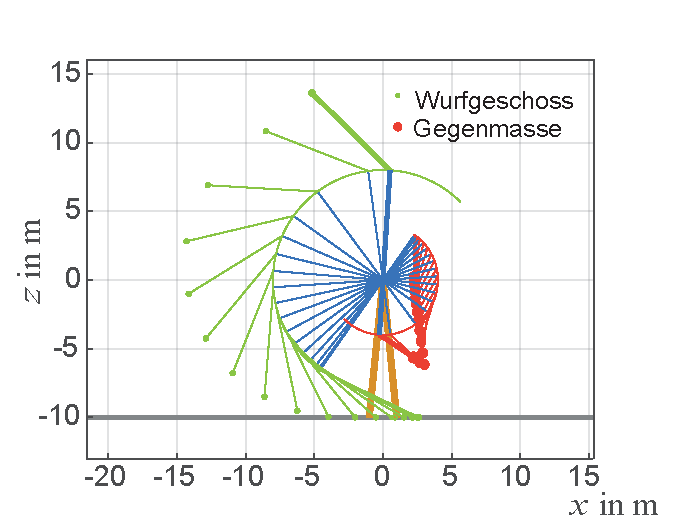
\includegraphics[width=0.5\textwidth]{TrebSim04b.pdf}}%
\hspace{\fill}
\rightfigure{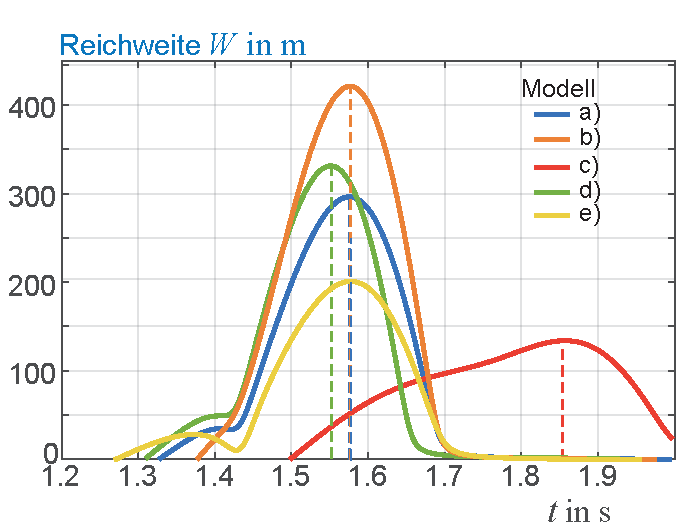
\includegraphics[width=0.5\textwidth]{TrebSim04a.pdf}}
\leftcaption[Dynamik eines Trebuchet unter Ber�cksichtigung einer Zwangsbedingung.]{Dynamik eines Trebuchet unter Ber�cksichtigung einer Zwangsbedingung.} \label{abb:bew_TrebErgebnis4b}
\rightcaption[Reichweite f�nf verschiedener Trebuchet.]{Reichweite f�nf verschiedener Trebuchet. Parameter siehe Tabelle \ref{tab:bew_trebuchet_03}.}
\label{abb:bew_TrebErgebnis4a}  
\end{minipage}
\end{figure}


\begin{table}
  \centering
  \begin{tabular}{|c|r|r|r|r|r@.l|r@.l|r@.l|r@.l|r@.l|r@.l|}
%  \begin{tabular}{|c|r|r|r|r|rl|rl|rl|rl|rl|rl|}
  \hline
  %\rule{0pt}{3pt}\\
  \phantom{x}&\phantom{x}&\phantom{x}&\phantom{x}&\phantom{x}&\multicolumn2{c|}{\phantom{x}}&\multicolumn2{c|}{\phantom{x}}&\multicolumn2{c|}{\phantom{x}}&\multicolumn2{c|}{\phantom{x}}&\multicolumn2{c|}{\phantom{x}}&\multicolumn2{c|}{\phantom{x}}\\
  Parameter & $l_\text{G}  $ & $l_\text{W}  $ & $B  $ & $b  $ & \multicolumn2{c|}{$ W  $} & \multicolumn2{c|}{$t_\text{abw} $}   & \multicolumn2{c|}{$\alpha   $} & \multicolumn2{c|}{$v_\text{abw}    $} & \multicolumn2{c|}{$\epsilon_\text{W}    $} & \multicolumn2{c|}{$\epsilon_\text{T}    $} \\
  Einheit   & $\si{\metre}$ & $\si{\metre}$ & $\si{\metre}$ &  $\si{\metre}$ & \multicolumn2{c|}{$ \si{\metre}$} & \multicolumn2{c|}{$\si{\second}$} & \multicolumn2{c|}{$ \si{\degree}$} & \multicolumn2{c|}{$\si{\metre\per\second} $} & \multicolumn2{c|}{$\si{\%}$} & \multicolumn2{c|}{$\si{\%}$} \\
  \phantom{x}&\phantom{x}&\phantom{x}&\phantom{x}&\phantom{x}&\multicolumn2{c|}{\phantom{x}}&\multicolumn2{c|}{\phantom{x}}&\multicolumn2{c|}{\phantom{x}}&\multicolumn2{c|}{\phantom{x}}&\multicolumn2{c|}{\phantom{x}}&\multicolumn2{c|}{\phantom{x}}\\
  %\rule{0pt}{3pt}\\
  \hline
  Fall   a) &          3 &          8 &          4 &           8 & 296&2 & 1&58 & 35&1 & 55&4 & 18&2 & 19&6 \\
  Fall   b) &          3 & \textbf{9} & \textbf{3} &  \textbf{9} & 427&0 & 1&60 & 34&8 & 66&7 & 38&0 & 41&5 \\
  Fall   c) &          3 &          8 & \textbf{2} & \textbf{10} & 133&1 & 1&86 & 26&4 & 40&2 & 20&9 & 27&3 \\
  Fall   d) & \textbf{4} &          8 &          4 &           8 & 327&2 & 1&57 & 33&9 & 58&8 & 20&7 & 22&7 \\
  Fall   e) &          3 & \textbf{7} &          4 &           8 & 198&5 & 1&58 & 32&3 & 46&3 & 12&1 & 13&6 \\
  \hline
  \end{tabular}
\medskip
\caption[Reichweiten und Effizienzparameter f�r verschiedene Trebuchet-Designs. Die Zwangsbedingung ist ber�cksichtigt.]{Reichweiten und Effizienzparameter f�r verschiedene Trebuchet-Designs. Die Zwangsbedingung ist ber�cksichtigt. Weitere Parameter: $h= \SI{10}{\metre}$, $m_\text{G} = \SI{10000}{\kilogram}$, $m_\text{W} = \SI{100}{\kilogram}$, $m_\text{T} = \SI{1040}{\kilogram}$. Die Berechnungen finden sich in den einzelnen \mscr en.} \label{tab:bew_trebuchet_03}
\end{table}

Zum Schluss geben wir noch die Erweiterung von \eqref{eq:bew_treb17} auf mehrere Zwangsbedingungen an.
Man erh�lt nach einfacher �berlegung
\begin{align}
		\begin{split}
		\lk \begin{array} {cc}
				\mathbb{M} ~~ & ~ \lek \frac{\d \vec{f}}{\d \vec{q}}\rek^\text{T}\\
				\frac{\d \vec{f}}{\d \vec{q}} ~~& ~ \vec{0} 
		\end{array} \rk \cdot 
		\lek \begin{array} {l}
				\ddot{\vec{q}}\\
				\vec{\lambda}
		\end{array} \rek &= 
		\lek \begin{array} {l}
				\vec{F}\\
				\vec{F}_\lambda
		\end{array} \rek \,, \label{eq:bew_treb17b}
		\end{split}
\end{align}
worin $\vec{\lambda} = (\lambda_1, \lambda_2, \ldots)$, $\vec{F}_\lambda = (F_{\lambda 1}, F_{\lambda 2}, \ldots)$ und $\d \vec{f}/\d \vec{q}$ die \emph{Jacobi}\indexp{Jacobi, Carl Gustav Jacob}\index{Jacobi-Matrix|textbf}\emph{-Matrix} ist (siehe Infokasten) und \cite{Andrews2003, Riley2006, Bartelmann2015}.\\
%\footnote{Carl Gustav Jacob Jacobi (1804--1851) war einer deutscher Mathematiker, der zu den produktivsten und vielseitigsten Mathematikern z�hlt.
%Besonders seine Theorie der elliptischen Funktionen, aber auch seine Arbeiten zur Differentialgeometrie waren f�r die mathematischen Physik wegbereitend.
%Die Hamilton-Jacobi-Theorie der klassischen Mechanik war eine wichtige Vorstufe f�r den sp�teren �bergang zur Quantenmechanik.}
\medskip
\fbox{\parbox{1.0\textwidth}{
\medskip
\textbf{\textit{Jacobi-Matrix}}\\
Die Jacobi-Matrix\indexp{Jacobi,Carl Gustav Jacob} wird auch Funktionalmatrix oder Ableitungsmatrix genannt) und ist eine $m \times n$\,-Matrix s�mtlicher erster partieller Ableitungen der $i=1 \ldots m$\, Komponenten einer Funktion $\vec{f}$ (also der $f_m$) nach den $j = 1 \ldots n$\, Variablen:
\begin{align}
\mathbb{J} =  \frac{\d f_j}{\d q_i} =
\begin{pmatrix}
  \frac{\d f_1}{\d q_1} & \frac{\d f_2}{\d q_1}& 
    \ldots & 
    \frac{\d f_{m-1}}{\d q_1} &\frac{\d f_m}{\d q_1} \\[2ex] % <-- 1ex more space between rows of matrix
  \frac{\d f_2}{\d q_1} & \frac{\d f_2}{\d q_2}&
    \ldots & 
    \frac{\d f_{m-1}}{\d q_2} &\frac{\d f_m}{\d q_2} \\[2ex] % <-- 1ex more space between rows of matrix
  \vdots&  & & & \vdots \\[2ex]
  \frac{\d f_1}{\d q_{n-1}} & \frac{\d f_2}{\d q_{n-1}}& 
    \ldots & 
    \frac{\d f_{m-1}}{\d q_{n-1}} &\frac{\d f_m}{\d q_{n-1}}\\[2ex]%
  \frac{\d f_1}{\d q_n} & \frac{\d f_2}{\d q_n} &
    \ldots & 
    \frac{\d f_{m-1}}{\d q_n} &\frac{\d f_m}{\d q_n} 
\end{pmatrix} \,. \label{eq:bew_Jacobi_function01}
\end{align} 
%\begin{align}
%\mathbb{J} = J_{i,j} =
%\begin{pmatrix}
  %\frac{\d f_1}{\d q_1} & 
    %\frac{\d f_1}{\d q_2} & 
    %\frac{\d f_1}{\d q_3} \\[1ex] % <-- 1ex more space between rows of matrix
  %\frac{\d f_2}{\d q_1} & 
    %\frac{\d f_2}{\d q_2} & 
    %\frac{\d f_2}{\d q_3} \\[1ex]
  %\frac{\d f_3}{\d q_1} & 
    %\frac{\d f_3}{\d q_2} & 
    %\frac{\d f_3}{\d q_3} 
%\end{pmatrix} \,. \label{eq:bew_Jacobi_function01}
%\end{align} 
Die Jacobi-Matrix findet weitreichende Anwendungen bei der Approximation und Extremwertberechnung mehrdimensionaler Funktionen und besonders auch bei Koordinatentransformationen.
So hat \zb die Jacobi-Matrix f�r die Koordinatentransformation von kartesischen $f_j =(x,y,z)$ in sph�rische $q_i =(r,\vartheta,\varphi)$ Koordinaten mit $i,j = 1 \ldots 3$ die folgende Form:
\begin{align}
\mathbb{J} = \frac{\d f_j}{\d q_i} = \begin{pmatrix} \sin\vartheta \cos\varphi & ~~r \cos\vartheta\cos\varphi &~~ -r \sin\vartheta\sin\varphi\\ \sin\vartheta \cos\varphi &~~ r \cos\vartheta\sin\varphi &~~ r \sin\vartheta\cos\varphi\\ \cos\vartheta &~~- r \sin\vartheta &~~ 0 \end{pmatrix} \,. \label{eq:bew_Jacobi_function02}
\end{align}
Da in diesem Fall die Jacobi-Matrix eine quadratische Matrix ist, l�sst sich deren Determinante berechnen. Diese wird Jacobi-Determinante genannt. Sie spielt bei der Koordinatentransformation von Integralen eine wichtige Rolle und die Berechnung des Volumenelements ergibt im vorliegenden Fall: 
%\begin{align}
 %\det\,\mathbb{J}(r,\vartheta,\varphi) = r^2\,\sin\vartheta\,. \label{eq:bew_Jacobi_function03}
%\end{align}
\begin{align}
 \D V = \D x \, \D y \, \D z \, =  \det \,\mathbb{J} \:\, \D r\,\D \vartheta\,\D \varphi = r^2\sin\vartheta\,\D r\,\D \vartheta\,\D \varphi\,. \label{eq:bew_Jacobi_function04}
\end{align}
}}

Ein Beispiel f�r ein Trebuchet mit mehreren Zwangsbedingungen ist in \probref{bew_Trebuchet_II} gegeben, die auf einer Arbeit von \cite{Constans2017} beruht.
Wir werden bei der L�sung bis zu vier Zwangsbedingungen bei f�nf generalisierten Koordinaten verarbeiten, so dass die Jacobi-Matrix $\d \vec{f}/\d \vec{q}$ die Dimension~$5\times4$ annehmen kann.\\
Wir haben mit diesem sch�nen und illustrativen Beispiel des Trebuchet noch einmal gezeigt, dass man mit dem Lagrange-Formalismus f�r Massepunkte recht komplexe Systeme sehr effizient beschreiben und numerisch behandeln kann.


\clearpage
%\clearpage
%\section{Tabellen}\label{kap:bew_tabellen}

\clearpage



\renewcommand\glslongextraNameAlign{p{36mm}}
\renewcommand\glslongextraDescAlign{p{60mm}}
\clearpage
\bgroup
\small
\printunsrtglossary[type=bew]
\egroup
\clearpage
\fancyhead[RE]{\nouppercase\rightmark}
\begingroup
\let\cleardoublepage\relax
\bibliography{referenzen}
\endgroup
\fancyhead[RE]{\nouppercase\leftmark}
%%%%%%%%%%%%%%%%%%%%%%%%%%%%%%%%%%%%%%%%%%%%%%%%%%%%%%%%%%%%%
%\input{footer.tex}

\addtocontents{toc}{\protect\setcounter{tocdepth}{-1}}% nichts zeigen bei ArbeitsbuchBook
%\documentclass[makeidx,envcountchap,graybox,deutsch,ngerman,sectrefs]{svmono}
%\documentclass[envcountchap,graybox,deutsch,sectrefs]{svmono}
%%%%% eigene tempor�re Abk�rzungsliste, f�r die Zeit, bis einheitliche Schreibungen bestehen
\usepackage{tempshort}
%%  Von Springer empfohlene Pakete %% 
%%\documentclass[envcountsect,graybox,deutsch,sectrefs]{svmono}
\usepackage{chapterbib}
\usepackage{type1cm}
\usepackage[ansinew]{inputenc}
\usepackage{babel}
\usepackage[pdftex]{graphicx} %PDF-Vektorgrafiken einbinden
\usepackage{newtxtext} %Typischer Springer-Font
\usepackage{newtxmath}
\usepackage{multicol}
\usepackage[bottom]{footmisc} %Platziert alle Fu�noten unten  
\usepackage[nobreak]{cite}
%\usepackage{biblatex}
\usepackage{cancel}
\usepackage[absolute]{textpos}
\usepackage{graphicx}
\usepackage{pdfpages}

%\usepackage{floatrow}
%\usepackage{mwe}
\usepackage[figuresright]{rotating}
\usepackage{bigints}
\let\laplace\relax  % Vermeidung der Fehlermeldung "\laplace already defined."
\usepackage{trfsigns}
\usepackage{amsmath}
\usepackage{tabulary}
\usepackage{tabularx}

%%  Eigene Pakete %%
\usepackage{adjustbox}
\usepackage{wasysym}
\usepackage{gensymb}
\usepackage{float}
\usepackage{caption}
\usepackage[left=5cm,right=4cm,top=3cm,bottom=4cm,includeheadfoot]{geometry}

%\usepackage{wasysym}
%\usepackage{bigints}
%\usepackage{esint}
%\usepackage{relsize,exscale}

\usepackage{mathtools}   % Vermeidung der Fehlermeldung "Undefined control sequence \coloneqq."


% header and footer
\usepackage{fancyhdr}
\pagestyle{fancy}
\fancyhead[LE,RO]\thepage
\renewcommand{\sectionmark}[1]{\markright{\thesection.\ #1}}
%\fancyhead[LO]{\nouppercase\leftmark}
%\fancyhead[RE]{\nouppercase\rightmark}
\fancyhead[LO]{\nouppercase\rightmark}
\fancyhead[RE]{\nouppercase\leftmark}
\fancyfoot{}
% svmono hat offenbar irgendwas merkw�rdig definiert, darum mu� hier verbreitert werden
%\addtolength\headwidth{25pt}
\setlength{\headheight}{25pt}

%% Units
\usepackage{siunitx}
\sisetup{
  locale = US,
  per-mode = reciprocal, %symbol, % | reciprocal | fraction | ?
  exponent-product = \cdot,
  separate-uncertainty,
  %exponent-to-prefix,
  %prefixes-as-symbols = false,
  %list-units = brackets,% | single | repeat
  %range-units = brackets,% | single | repeat
  %multi-part-units = brackets,% | single | repeat
}
\usepackage{chngcntr}
\usepackage{booktabs}
\usepackage{slashed}
\usepackage{listings}
\usepackage{color} %red, green, blue, yellow, cyan, magenta, black, white
%\usepackage{color} %Einfache Farbendefinition -> von Graybox-Option ben�tigt
\usepackage{multirow}
\usepackage{longtable} %Tabellen �ber mehrere Seiten hinweg
\usepackage{framed} % von Graybox-Option ben�tigt
\usepackage[shortlabels]{enumitem} %Erweiterte Aufz�hloptionen
\usepackage{array}
\usepackage[xindy]{imakeidx} %Wortindex und Personenindex erstellen

\usepackage[hyphens]{url}
%\usepackage[breaklinks,colorlinks=true,linkcolor=black,urlcolor=blue,citecolor=black,filecolor=green,hyperfootnotes=false]{hyperref}
\usepackage[                                    %Hyperref erstellt ein Bookmark/Lesezeichen im PDF. siehe https://www.namsu.de/Extra/pakete/Hyperref.html
bookmarksopen=true,															%Das Lesezeichen ist ge�ffnet beim �ffnen der PDF.
bookmarksnumbered=true,                         %Zahlen werden im Bookmark angezeigt.   
plainpages=false,
pdfpagelabels,
colorlinks=true,                                %Links werden farbig dargestellt.
linkcolor=black, citecolor=black, urlcolor=cyan %Farben definieren.
]{hyperref}                                     %Sollte als letztes eingebunden werden, da es sehr viele Verweise und �nderungen erzeugt. Das Packet ist sehr stark, aber auch umfangreich ist. 

%\usepackage[breaklinks,colorlinks=true,linkcolor=black,urlcolor=blue,citecolor=black,filecolor=green,hyperfootnotes=false]{hyperref}
%\usepackage[breaklinks,colorlinks=true,linkcolor=black,urlcolor=blue,citecolor=black,filecolor=green,hyperfootnotes=false
            %pdftex,
            %pdfauthor={Kaschke, Cartarius},
            %pdftitle={Finger�bungen der Physik}
            %pdfsubject={Ein Repetitorium und �bungsbuch zu im Studium wenig behandelten Kapiteln der Physik mit ausf�hrlich behandelten Problemen und MATLAB-Programmen},
            %pdfkeywords={Physik, Mechanik}
            %]{hyperref}
\pdfminorversion=5

\usepackage{hypcap}
\usepackage[record,section=section,stylemods={mcols},automake]{glossaries-extra}
\usepackage{glossary-longextra}
%\usepackage{glossary-bookindex}
%\makeindex
\setglossarystyle{long-name-sym-desc-loc}
\setabbreviationstyle[acronym]{long-short}

\definecolor{killA}{rgb}{.7,.3,.3}
\newcommand\killA[1]{\bgroup\color{killA}{\cancel{#1}}\egroup}
\newcommand\killB[1]{\bgroup\color{cyan!30!black}{\cancel{#1}}\egroup}

% typographisch korrekte Abk�rzungen (needs to be loaded after hyperref)
\usepackage{abbrev}
\newglossary*{bew}{Glossar}
\newglossary*{hm}{Glossar}
\newglossary*{adyn}{Glossar}
\newglossary*{kontmech}{Glossar}
\newglossary*{aero}{Glossar}
\newglossary*{edyn}{Glossar}
\newglossary*{spo}{Glossar}
\newglossary*{optbas}{Glossar}
\newglossary*{optger}{Glossar}
\newglossary*{optatm}{Glossar}
\newglossary*{optspez}{Glossar}
\GlsXtrLoadResources[src={bew/gloss},type=bew]
\GlsXtrLoadResources[src={hm/gloss},type=hm]
\GlsXtrLoadResources[src={adyn/gloss},type=adyn]
\GlsXtrLoadResources[src={kontmech/gloss},type=kontmech]
\GlsXtrLoadResources[src={aero/gloss},type=aero]
\GlsXtrLoadResources[src={spo/gloss},type=spo]
\GlsXtrLoadResources[src={edyn/gloss},type=edyn]
\GlsXtrLoadResources[src={optbas/gloss},type=optbas]
\GlsXtrLoadResources[src={optger/gloss},type=optger]
\GlsXtrLoadResources[src={optatm/gloss},type=optatm]
\GlsXtrLoadResources[src={optspez/gloss},type=optspez]
\glssetcategoryattribute{bew}{indexname}{true}
%\renewcommand\index\newterm
%\newcolumntype{g}[1]{>{\RaggedRight\hspace{0pt}}p{#1}}
%\renewcommand\glslongextraNameAlign{g}
\renewcommand\glslongextraLocationAlign{@{\ ~\ }>{\raggedright}p{\glspagelistwidth}}
\definecolor{gls}{rgb}{.4,.4,.5}
\renewcommand*{\glstextformat}[1]{\textcolor{gls}{#1}}

%Absatzregeln
\clubpenalty = 30000 %Keine einzelnen Absatzzeilen
\widowpenalty = 30000
\setlength{\parindent}{0em} 
\newcolumntype{L}[1]{>{\raggedright\arraybackslash}p{#1}}
\newcolumntype{C}[1]{>{\centering\arraybackslash}p{#1}}
\newcolumntype{R}[1]{>{\raggedleft\arraybackslash}p{#1}}

\usepackage{xstring}

\newcommand\mfile[2]{%
\saveexpandmode\noexpandarg
\StrSubstitute{#2}{_}{\_}[\tmpname]
\restoreexpandmode
\href{MatlabDateien/\chapname/#1\tmpname}{\tmpname}}

%%% Hyperlinks zu MATLAB Dateien
%\newcommand\mlref[1]{\mfile{}{#1}}
%\newcommand\mlinclref[1]{\mfile{IncludeFolder/}{#1}}
%\newcommand\mldataref[1]{\mfile{Data/}{#1}}

%%% .. f�r ein Verzeichnis hoch
%%% . f�r aktuelle Verzeichnis
%% lokal: MatlabDateien/bew
%\newcommand\mlbewref[1]{\href{MatlabDateien/bew/#1}{#1}}
%% git: https://github.com/sn-code-inside/fingeruebungen-physik/tree/main/bew

\newcommand{\mlrefwithindex}[2]{%
  \index[mfiles]{#2}%   <-- Eintrag im M-File-Index mit aktueller Seitenzahl
  \href{https://github.com/sn-code-inside/fingeruebungen-physik/tree/main/#1/#2}{#2}%
}


%\newcommand\mlbewref[1]{\href{https://github.com/sn-code-inside/fingeruebungen-physik/tree/main/bew/#1}{#1}}
%\newcommand\mlbewdref[1]{\href{https://github.com/sn-code-inside/fingeruebungen-physik/tree/main/bew/Data/#1}{#1}}
%\newcommand\mlbewiref[1]{\href{https://github.com/sn-code-inside/fingeruebungen-physik/tree/main/bew/IncludeFolder/#1}{#1}}
%\newcommand\mlkontmechref[1]{\href{https://github.com/sn-code-inside/fingeruebungen-physik/tree/main/kontmech/#1}{#1}}
%\newcommand\mlkontmechdref[1]{\href{https://github.com/sn-code-inside/fingeruebungen-physik/tree/main/kontmech/Data/#1}{#1}}
%\newcommand\mlkontmechiref[1]{\href{https://github.com/sn-code-inside/fingeruebungen-physik/tree/main/kontmech/IncludeFolder/#1}{#1}}
%\newcommand\mlhmref[1]{\href{https://github.com/sn-code-inside/fingeruebungen-physik/tree/main/hm/#1}{#1}}
%\newcommand\mlhmdref[1]{\href{https://github.com/sn-code-inside/fingeruebungen-physik/tree/main/hm/Data/#1}{#1}}
%\newcommand\mlhmiref[1]{\href{https://github.com/sn-code-inside/fingeruebungen-physik/tree/main/hm/IncludeFolder/#1}{#1}}
%\newcommand\mladynref[1]{\href{https://github.com/sn-code-inside/fingeruebungen-physik/tree/main/adyn/#1}{#1}}
%\newcommand\mladyndref[1]{\href{https://github.com/sn-code-inside/fingeruebungen-physik/tree/main/adyn/Data/#1}{#1}}
%\newcommand\mladyniref[1]{\href{https://github.com/sn-code-inside/fingeruebungen-physik/tree/main/adyn/IncludeFolder/#1}{#1}}
%\newcommand\mledynref[1]{\href{https://github.com/sn-code-inside/fingeruebungen-physik/tree/main/edyn/#1}{#1}}
%\newcommand\mledyndref[1]{\href{https://github.com/sn-code-inside/fingeruebungen-physik/tree/main/edyn/Data/#1}{#1}}
%\newcommand\mledyniref[1]{\href{https://github.com/sn-code-inside/fingeruebungen-physik/tree/main/edyn/IncludeFolder/#1}{#1}}
%\newcommand\mloptbasref[1]{\href{https://github.com/sn-code-inside/fingeruebungen-physik/tree/main/optbas/#1}{#1}}
%\newcommand\mloptbasdref[1]{\href{https://github.com/sn-code-inside/fingeruebungen-physik/tree/main/optbas/Data/#1}{#1}}
%\newcommand\mloptbasiref[1]{\href{https://github.com/sn-code-inside/fingeruebungen-physik/tree/main/optbas/IncludeFolder/#1}{#1}}
%\newcommand\mloptspezref[1]{\href{https://github.com/sn-code-inside/fingeruebungen-physik/tree/main/optspez/#1}{#1}}
%\newcommand\mloptspezdref[1]{\href{https://github.com/sn-code-inside/fingeruebungen-physik/tree/main/optspez/Data/#1}{#1}}
%\newcommand\mloptspeziref[1]{\href{https://github.com/sn-code-inside/fingeruebungen-physik/tree/main/optspez/IncludeFolder/#1}{#1}}

\newcommand\mlbewref[1]{\mlrefwithindex{bew}{#1}}
\newcommand\mlbewdref[1]{\mlrefwithindex{bew/Data}{#1}}
\newcommand\mlbewiref[1]{\mlrefwithindex{bew/Include}{#1}}
\newcommand\mlkontmechref[1]{\mlrefwithindex{kontmech}{#1}}
\newcommand\mlkontmechdref[1]{\mlrefwithindex{kontmech/Data}{#1}}
\newcommand\mlkontmechiref[1]{\mlrefwithindex{kontmech/Include}{#1}}
\newcommand\mlhmref[1]{\mlrefwithindex{hm}{#1}}
\newcommand\mlhmdref[1]{\mlrefwithindex{hm/Data}{#1}}
\newcommand\mlhmiref[1]{\mlrefwithindex{hm/Include}{#1}}
\newcommand\mladynref[1]{\mlrefwithindex{adyn}{#1}}
\newcommand\mladyndref[1]{\mlrefwithindex{adyn/Data}{#1}}
\newcommand\mladyniref[1]{\mlrefwithindex{adyn/Index}{#1}}
\newcommand\mledynref[1]{\mlrefwithindex{edyn}{#1}}
\newcommand\mledyndref[1]{\mlrefwithindex{edyn/Data}{#1}}
\newcommand\mledyniref[1]{\mlrefwithindex{edyn/Index}{#1}}
\newcommand\mloptbasref[1]{\mlrefwithindex{optbas}{#1}}
\newcommand\mloptbasdref[1]{\mlrefwithindex{optbas/Data}{#1}}
\newcommand\mloptbasiref[1]{\mlrefwithindex{optbas/Include}{#1}}
\newcommand\mloptspezref[1]{\mlrefwithindex{optspez}{#1}}
\newcommand\mloptspezdref[1]{\mlrefwithindex{optspez/Data}{#1}}
\newcommand\mloptspeziref[1]{\mlrefwithindex{optspez/Include}{#1}}
\newcommand\mloptgerref[1]{\mlrefwithindex{optger}{#1}}
\newcommand\mloptgerdref[1]{\mlrefwithindex{optger/Data}{#1}}
\newcommand\mloptgeriref[1]{\mlrefwithindex{optger/Include}{#1}}
\newcommand\mloptatmref[1]{\mlrefwithindex{optatm}{#1}}
\newcommand\mloptatmdref[1]{\mlrefwithindex{optatm/Data}{#1}}
\newcommand\mloptatmiref[1]{\mlrefwithindex{optatm/Include}{#1}}



\newcommand\mlcmd[1]{\textcolor{cyan}{\texttt{#1}}}

%Grafikregeln
\graphicspath{{hm/graphs/}
	                    	{bew/graphs/}
     						{kontmech/graphs/}
							{hm/graphs/}
							{adyn/graphs/}
							{edyn/graphs/}
							{kontmech/graphs/}
							{spo/graphs/}
							{optbas/graphs/}
							{optger/graphs/}
							{optatm/graphs/}
							{solman/graphs/}
                                                        {aero/graphs}}
\DeclareGraphicsExtensions{.pdf, .png, .jpg, .jpeg}
\def\figname{Abb}
\newcommand\figref[1]{\figname.\ \ref{abb:#1}}
\usepackage[labelfont=bf]{caption}

\usepackage{tocloft}
\usepackage{etoc}
\setlength\cftfignumwidth{30pt}

% Flatterrand links
\cftsetindents{chapter}{0em}{4em}
\cftsetindents{section}{1.5em}{4em}
\cftsetindents{subsection}{3.8em}{4em}

% flacher Rand links
%\cftsetindents{chapter}{0em}{4em}
%\cftsetindents{section}{0em}{4em}
%\cftsetindents{subsection}{0em}{4em}

\newcommand\partitle[1]{
\addcontentsline{toc}{part}{#1}
\begin{titlepage}
  %\vskip 60%\p@
  \begin{center}
    {\LARGE Finger�bungen der Physik -- #1 \par}
    \vskip 3em%
    {\large Michael Kaschke und Holger Cartarius\par}
  \end{center}
\end{titlepage}
}

%\newcommand\mlref[1]{\href{\chapname/matlab/#1}{#1}}
%\newcommand\mlinclref[1]{\href{\chapname/matlab/IncludeFolder/#1}{\color{cyan}{#1}}}

%Neue Kommandos
\newcommand{\lk}{\left(}        %gro�e runde Klammer (links)
\newcommand{\rk}{\right )}      %gro�e runde Klammer (rechts)
\newcommand{\lgk}{\left \{}     %gro�e geschweifte Klammer (links)
\newcommand{\rgk}{\right \}}    %gro�e geschweifte Klammer (rechts)
\newcommand{\lek}{\left [}      %gro�e eckige Klammer (links)
\newcommand{\rek}{\right ]}     %gro�e eckige Klammer (rechts)
\newcommand{\anf}[1]{\glqq#1\grqq}    %Deutsche Anf�hrungszeichen: \anf{}
\newcommand{\defined}{:=}				%Definition
\newcommand{\curl}{\text{\textbf{rot}}\,}	%Rotation-Operator curl()
\newcommand{\ket}[1]{|#1\rangle}		%Quantenmechanischer Zustand
\newcommand{\curvelintri}{\,\overset{\blacktriangle}{\smallfrown}}
\newcommand{\straighttri}{\blacktriangle}
\newcommand{\UT}{\text{UT}}
\newcommand{\UTC}{\text{UTC}}
\newcommand{\JD}{\text{JD}}
\newcommand{\JDE}{\text{JDE}}
\newcommand{\MJD}{\text{MJD}}
\newcommand{\TDT}{\text{TDT}}
\newcommand{\TT}{\text{TT}}
\newcommand{\NVS}{\text{Navier-Stokes-Gleichungen}}
\newcommand{\MWG}{\text{Maxwell-Gleichungen}}
\newcommand{\EMW}{\text{Elektromagnetische Wellen}}
\newcommand{\eMW}{\text{elektromagnetischen Wellen}}
\newcommand{\RT}{\text{Relativit�tstheorie~}}
\newcommand{\au}{\mathrm{AE}}
\newcommand{\ET}{\text{ET}}
\newcommand{\TAI}{\text{TAI}}
\newcommand{\GMST}{\text{GMST}}
\newcommand{\LMST}{\text{LMST}}
\newcommand{\MESZ}{\text{MESZ}}
\newcommand{\KOS}{\text{Koordinatensystem }}
\newcommand{\DGL}{\text{Differentialgleichung }}
\newcommand{\NA}{\text{NA}}
\newcommand{\uA}{\text{u}}  %atomare Masseneinheit
\newcommand{\MOZ}{\text{MOZ}}
\newcommand{\grad}{\text{\textbf{grad}}\,}	%Gradient-Operator grad()
\newcommand{\uproman}[1]{\mathrm{\uppercase\expandafter{\romannumeral#1}}}
\newcommand{\lowroman}[1]{\romannumeral#1\relax}

\newcommand\todo[1]{\textcolor{red}{TODO: #1}}

\renewcommand{\=}[1]{\stackrel{\text{#1}}{=}}  %Schrift �ber Gleich-Zeichen
\renewcommand{\d}{\partial}
\newcommand{\lra}{\Leftrightarrow}  %�quivalenz-Pfeile
\newcommand{\abs}[1]{\left\vert#1\right\vert}     %Betragsklammern
\renewcommand{\Re}{\mathrm{Re}}                          %Realteil
\renewcommand{\Im}{\mathrm{Im}}                          %Imagin�rteil
\renewcommand{\im}{\mathrm{i}}                         %Imagin�re Einheit
\renewcommand{\epsilon}{\varepsilon} 
\newcommand{\keff}{k_\text{eff}}
\newcommand{\con}{\text{const}}
\newcommand{\conv}{\vec{const}}
\newcommand{\PL}{\mathcal{P}_}
\newcommand{\artanh}{\mathrm{artanh}}
% QED-Symbol im text- bzw. Mathemodus
\newcommand{\textqed}{\hfill ~ $\square$}
\newcommand{\mmqed}{\tag*{$\square$}}

\newcommand{\fa}{(\textbf{a}) }
\newcommand{\fb}{(\textbf{b}) }
\newcommand{\fc}{(\textbf{c}) }
\newcommand{\fd}{(\textbf{d}) }
\newcommand{\fe}{(\textbf{e}) }
\newcommand{\ff}{(\textbf{f}) }

\newcommand{\iF}{im Folgenden~}
\newcommand{\iA}{im Allgemeinen~}


\DeclareMathOperator\divv{div}
\DeclareMathOperator\res{Res}
\DeclareMathOperator{\sech}{sech}
\DeclareMathOperator\sgn{sgn}

% f�r Appendix - MATLAB Referenz
\newcommand{\rotv}{\vec{rot}\,}
\newcommand{\gradv}{\vec{grad}\,}
\newcommand{\nablav}{\vec{\nabla}\,}

\newcommand{\ceil}{\mathrm{ceil}}
\newcommand{\sinc}{\mathrm{sinc}}
\newcommand{\diag}{\mathrm{diag}}
\newcommand{\sign}{\mathrm{sign}}
\newcommand{\length}{\mathrm{length}}
\newcommand{\sort}{\mathrm{sort}}
\newcommand{\summ}{\mathrm{sum}}
\newcommand{\asin}{\mathrm{asin}}
\newcommand{\acos}{\mathrm{acos}}
\newcommand{\atan}{\mathrm{atan}}
\newcommand{\prodd}{\mathrm{prod}}
\newcommand{\median}{\mathrm{mediab}}
\newcommand{\mean}{\mathrm{mean}}
\newcommand{\std}{\mathrm{std}}
\newcommand{\eye}{\mathrm{eye}}
\newcommand{\zeros}{\mathrm{zeros}}
\newcommand{\ones}{\mathrm{ones}}
\newcommand{\rand}{\mathrm{rand}}
\newcommand{\inline}{\mathrm{inline}}
\newcommand{\modd}{\mathrm{mod}}
\newcommand{\floor}{\mathrm{floor}}
\newcommand{\round}{\mathrm{round}}
\newcommand{\rem}{\mathrm{rem}}
\newcommand{\sqrtt}{\mathrm{sqrt}}
\newcommand{\triu}{\mathrm{triu}}
\newcommand{\tril}{\mathrm{tril}}
\newcommand{\size}{\mathrm{size}}
\newcommand{\dett}{\mathrm{det}}
\newcommand{\inv}{\mathrm{inv}}
\newcommand{\rank}{\mathrm{rank}}
\newcommand{\rref}{\mathrm{rref}}
\newcommand{\eig}{\mathrm{eig}}
\newcommand{\poly}{\mathrm{poly}}
\newcommand{\lu}{\mathrm{lu}}
\newcommand{\qr}{\mathrm{qr}}
\newcommand{\quaddd}{\mathrm{quad}}
\newcommand{\fzero}{\mathrm{fzero}}
\newcommand{\roots}{\mathrm{roots}}
\newcommand{\odezd}{\textcolor{mygreen}{\texttt{ode23}}}
\newcommand{\odevf}{\textcolor{mygreen}{\texttt{ode45}}}
\newcommand{\odeeds}{\textcolor{mygreen}{\texttt{ode13s}}}
\newcommand{\odeefs}{\textcolor{mygreen}{\texttt{ode15s}}}
\newcommand{\ddezd}{\textcolor{mygreen}{\texttt{dde23}}}
\newcommand{\onlineZ}{online verf�gbaren Zusatzmaterialien{}}
\newcommand{\MKc}{\url{https://www.fingeruebungen-physik.de}{}}
\newcommand{\linklsg}{\href{https://www.fingeruebungen-physik.de}{\textcolor{blue} {$\rightarrow$ L�sungsteil.}}}
\newcommand{\githubSN}{\url{https://github.com/sn-code-inside/fingeruebungen-physik}{}\,\,}

\newcommand{\FT}{\mathcal{F}} %Fourier-Transformierte

% Aufz�hlung der L�sungen der Teilaufgaben
\newlist{subprobs}{enumerate}{1}
\setlist[subprobs]{
  label= \textbf{\textit{Teilaufgabe}} \textbf{\textit{\arabic*:}} \protect\thissubprob,
  ref=\arabic*, itemsep=\baselineskip, align=left}
\newcommand{\subprob}[1]{
  \def\thissubprob{\textbf{\textit{#1}}}\item ~\vspace{0.2\baselineskip} \newline}

\renewenvironment{example}[1]{
\refstepcounter{example}\par\medskip
\begin{shaded} 
\begin{samepage}
\noindent \textbf{\textit{Beispiel~\theexample: {#1}}}\\ 
\noindent{\color{black} \rule{\textwidth}{0.2 mm}}
\end{samepage}
}{\end{shaded}
\noindent{\color{black} \rule{\textwidth}{0.2 mm}}
} % or snugshade
\definecolor{shadecolor}{gray}{0.95}
\definecolor{mygreen}{RGB}{28,172,0} % color values Red, Green, Blue
\definecolor{mylilas}{RGB}{170,55,241}

\newenvironment{infobox}[1]{
     \begin{shaded} 
     \begin{samepage}
\noindent{\color{black} \rule{\textwidth}{0.2 mm}}
     \end{samepage}
}{\end{shaded}
\noindent{\color{black} \rule{\textwidth}{0.2 mm}}
} 
\definecolor{shadecolor}{gray}{0.95}
\definecolor{mygreen}{RGB}{28,172,0} % color values Red, Green, Blue
\definecolor{mylilas}{RGB}{170,55,241}


\newenvironment{nebenrechnung}[1]{
\begin{shaded} 
\begin{samepage}
\noindent\textbf{Nebenrechnung: \\} 
\noindent{\color{black} \rule{0.1\columnwidth}{0.2mm} \\}
\end{samepage}
}{\end{shaded}
\noindent{\color{black} \rule{0.1\columnwidth}{0.2mm} \\}
} % or snugshade
\definecolor{shadecolor}{gray}{0.95}
\definecolor{mygreen}{RGB}{28,172,0} % color values Red, Green, Blue
\definecolor{mylilas}{RGB}{170,55,241}

\newenvironment{merksatz}[1]{
\begin{shaded} 
\begin{samepage}
\noindent\textbf{Merke:\\} 
\noindent{\color{black} \rule{0.9\columnwidth}{0.2mm} \\ \\}
\end{samepage}
}{\end{shaded}
\noindent{\color{black} \rule{0.9\columnwidth}{0.2mm} \\}
} % or snugshade


\lstset{language=Matlab,%
    %basicstyle=\color{red},
    %basicstyle={\linespread{0.9}\ttfamily},
    basicstyle=\footnotesize\ttfamily,
    breaklines=true,%
    morekeywords={matlab2tikz},
    keywordstyle={\small \color{mygreen}},%
    morekeywords=[2]{1}, keywordstyle=[2]{\small\color{black}},
    identifierstyle={\small \color{black}},%
    stringstyle={\small\color{mylilas}},
    commentstyle={\small\color{mylilas}},%
    showstringspaces=false,%without this there will be a symbol in the places where there is a space
    numbers=left,%
    numberstyle={\tiny \color{black}},% size of the numbers
    numbersep=9pt, % this defines how far the numbers are from the text
    emph=[1]{for,end,else,break, function},emphstyle=[1]\small \color{blue}, %some words to emphasise
    emph=[2]{odeset},emphstyle=[2]\small \color{mygreen}, %some words to emphasise
    %emph=[2]{word1,word2}, emphstyle=[2]{style},    
}

%\bibliographystyle{spphys.bst}

%Trennregeln f�r spezielle Worte
%\hyphenation{Fresnel \matlab �qui-nok-ti-um}

\DeclareSIUnit\erg{erg}
\DeclareSIUnit\cal{cal}
\DeclareSIUnit\celsius{C}
\DeclareSIUnit\m{M}
\DeclareSIUnit\kel{K^{-4}}

%Stichwort- und Personenverzeichnis
\makeindex[title=Stichwortverzeichnis] % Create the default index
\makeindex[name=personen,title=Personenverzeichnis] % Create an index named 'personen'
\newcommand{\indexp}[1]{\index[personen]{#1}}
\makeindex[name=mfiles,title=MATLAB-Skriptverzeichnis,columns=2]

% list of exercises
\newcommand{\loxname}{\Large �bungsverzeichnis}  % einheitliche Gr��e Large
\newlistof[chapter]{prob}{lox}\loxname
\newcommand\uebung[3][]{\label{prob:#2}%
\addcontentsline{lox}{prob}{\protect\numberline{}{\probRef{#2}:~#3#1}}%
\textbf{#1#3}\\[\baselineskip]}
\makeatletter
\renewcommand{\l@prob}{\@dottedtocline{1}{0em}{0em}}
\makeatother

\newcommand\einfach{\uebung[~$\ast$~~]}
\newcommand\mittel{\uebung[~$\ast\,\ast$~~]}
\newcommand\schwierig{\uebung[~$\ast\,\ast\,\ast$~~]}
\newcommand\zusatz{\uebung[~$\ast\,\ast\,\ast\,!$~~]}
%\newcommand\einfach{\uebung[~\textbf{*}~~]}
%\newcommand\mittel{\uebung[~\textbf{*\,*}~~]}
%\newcommand\schwierig{\uebung[~\textbf{*\,*\,*}~]}
%\newcommand\zusatz{\uebung[~\textbf{*\,*\,*\,!}~~]}
\usepackage[atend]{bookmark}
%\BookmarkAtEnd{%
%\bookmarksetup{startatroot}\bookmark[level=0,named=\loxname]{}}

\newcommand\kapitel[1]{Kapitel \ref{kap:#1}}
%\newcommand\kap[1]{Kap.\ \ref{kap:#1}}
\newcommand\kap[1]{Kap. \ref{kap:#1}}

\begin{document}
% customize prob and sol in svmono
\makeatletter
%\counterwithin*{chapter}{part}

\spn@wtheorem{prob}{\bgroup\exercisename\egroup}{\bfseries}{\rmfamily}
\makeatother
\renewenvironment{sol}[1]{\par\addvspace{6pt}\noindent\phantomsection{\textbf{L�sung \ref{#1}}} \ignorespaces}{\par\addvspace{6pt}}
\newcommand\probRef[1]{�bung \ref{prob:#1}}
\renewcommand\probref[1]{\textbf{\probRef{#1}}}
\newcommand\lsgref[1]{L�sung \ref{lsg:#1}}

\newcommand\sbullet[1][.5]{\mathbin{\vcenter{\hbox{\scalebox{#1}{$\bullet$}}}}}

\setcounter{table}{0}


%%%%%%%%%%%%%%%%%%%%%%%%%%%%%%%%%%%%%%%%%%%%%%%%%%%%%%%%%%%%%
\chapter{Physik des Kontinuums}\label{chap:kontmech}
\def\chapname{kontmech}
\bibliographystyle{spphys}
%\begin{bibunit}[spphys]
\begin{minipage}{0.5\textwidth}
\includegraphics[width=\textwidth]{KontmechMotiv.pdf}
\end{minipage}
\medskip
\begin{minipage}{0.5\textwidth}
\begin{flushright}
\small
\emph{Schimpflich ist es, nicht zu gehen, \\
sondern sich treiben zu lassen und mitten \\
im Wirbel der Dinge verbl�fft zu fragen:\\
 Wie bin ich blo� hierher gekommen?\\}
\medskip
Seneca d.J. (1--65 n.Chr.)\\
\medskip
\medskip
\medskip
\medskip
\small
\emph{Alles in der Welt geht in der Wellenlinie.\\
Jede Landstra�e und so weiter. \\
Wehe dem, der �berall das Lineal anlegt!\\}
\medskip
Wilhelm Raabe (1831--1910)\\
%\emph{Die Welle beugt sich jedem Winde gern.\\}
%\medskip
%Johann Wolfgang von Goethe (1749--1832)\\
\medskip
\medskip
\normalsize
\end{flushright}
\end{minipage}

\section{Motivation}\label{kap:kontmech_motivation}

Die Kontinuumsmechanik und insbesondere die Hydro- und Aerodynamik (oft zusammen gefasst als Fluiddynamik\index{Fluiddynamik}) geh�ren zu den wichtigsten makroskopischen Theorien. Sie haben zahlreiche Anwendungen in vielen natur- und ingenieurwissenschaftlichen Disziplinen. Als Beispiele seien die Kosmologie, die Meteorologie, die Luft- und Raumfahrt, sowie Umweltwissenschaften, wie die Klimatologie und Ozeanographie genannt. Die Fluiddynamik wird trotz dieser breiten Anwendungsbereiche von Physikern und Ingenieuren h�ufig untersch�tzt und findet sich vielfach auch nicht entsprechend im Physikcurriculum wieder \cite{Lohse2023}. Dabei hat sich gerade bei den (numerischen) Methoden in den letzten 25 Jahren viel getan. Heute sind Dank der verf�gbaren Rechenleistungen Berechnungen und Simulationen m�glich, die vor Jahren noch bestenfalls in einem Hochleistungsrechenzentrum realisiert werden konnten. 

Aus diesen Gr�nden haben wir das Kapitel Physik des Kontinuums mit in den Band I der \textit{Physikalischen Finger�bungen} aufgenommen und werden dazu die Ans�tze der Mechanik ein weiteres Mal erweitern.
In \kap{bew_starrer_koerper} hatten wir bereits den starren K�rper eingef�hrt, der die Mechanik von Massepunkten um eine endliche Ausdehnung von K�rpern erweitert hat. Der K�rper hat jedoch seine Form behalten und die Bewegung konnte auf sechs Freiheitsgrade beschr�nkt werden.
Kann sich jedoch die Form eines K�rpers ver�ndern, gehen wir zur Kontinuumsmechanik �ber, die auch diese M�glichkeit abdeckt.
Insbesondere Gase und Fl�ssigkeiten, wir werden diese unter dem Begriff Fluide\index{Fluide} zusammenfassen, sind beliebig verformbar. Wollen wir ihre Bewegungen oder Str�mungen beschreiben, m�ssen wir auf Theorie des Kontinuums, in diesem Fall die Kontinuumsmechanik, zur�ckgreifen.

Eine Kontinuumstheorie\index{Kontinuumstheorie} gibt eine Beschreibung von Vielteilchensystemen durch gegebenenfalls zu definierende makroskopische physikalische Gr��en wie Dichte, Fl�sse, Geschwindigkeiten usw. Sie stellt insofern ein gemittelte Charakterisierung des Vielteilchensystems dar. Wir sind ja aber auch gar nicht an der mikroskopischen Dynamik des aus \ca $\SI{1e23}{}$ oder mehr Teilchen bestehenden Systems interessiert, denn die Beobachtung des Systems findet ja auf L�ngenskalen im sub-mm bis km-Bereich und auf Zeitskalen im sub-ms bis Stundenbereich statt, w�hrend die Dynamik der Einzelteilchen in Skalenbereichen von $\SI{}{\nano\metre}$ \bzw $\SI{e-14}{\second}$ abl�uft. Die Grundannahme einer Kontinuumstheorie besteht darin, dass man die langsamen und schnellen Prozesse voneinander separieren kann. So k�nnen wir f�r die Raumkoordinaten einen Volumenbereich definieren (das Volumenelement oder Fl�ssigkeitselement),\index{Volumenelement}\index{Fl�ssigkeitselement} �ber den die mikroskopischen Strukturen hinreichend ausgemittelt sind, im makroskopischen Beobachtungsbereich aber noch eine Variation von physikalischen Gr��en �ber die Raumkoordinaten beobachtet werden kann. Analoges gilt f�r die Zeitskala. 
F�r Zeiten, die deutlich gr��er sind als die Sto�zeiten (Zeit zwischen zwei St��en von Teilchen des Systems) k�nnen die auf eine Volumenelement wirkenden Kr�fte durch makroskopische Gr��en wie \zb Druck beschrieben werden. 
Das Volumenelement ist dann auf dieser makroskopischen Zeitskala lokal in einem mechanischen und auch thermischen Gleichgewichtszustand, so dass die Dynamik durch Differentialgleichungen mit nach Zeit und Raum getrennten Ableitungen beschrieben werden kann. Diese zeitliche und r�umliche Entwicklung von Dichten $\varrho(\vec{r},t)$ und Geschwindigkeitsprofilen $\vec{v}(\vec{r},t)$ und anderen Gr��en von Volumenelementen (Fl�ssigkeitselementen) unter der Wirkung von makroskopisch beschriebenen internen Kr�ften (\zb Druck) und externen Kr�ften (\zb der Schwerkraft) ist Gegenstand der im folgenden behandelten Mechanik der Kontinua.\\

Wir hatten bisher im Kapitel 1 im Wesentlichen die Bewegung und Dynamik von Massepunkten, Systemen von Massepunkten und Festk�rpern untersucht. Mathematisch f�hrte die Berechnung der zeitlichen Entwicklung der Raumkoordinaten und Geschwindigkeiten auf die L�sung von \textit{gew�hnlichen Differentialgleichungen} (GDGL) oder Systemen derselben. Im Fall des Kontinuums f�hren die Betrachtungen wegen der Ver�nderlichkeit der relativen Koordinaten von Massepunkten des Kontinuums zueinander und wegen der zeitlichen Ver�nderung der das Fluid kennzeichnenden physikalischen Gr��en auf Differentialgleichungen, die sowohl Ableitungen nach der Zeit als auch nach den Raumkoordinaten beinhalten, die man als \textit{partielle Differentialgleichungen} (PDGL) bezeichnet. Wir werden sehen, dass diese wesentlich komplexer und schwieriger zu l�sen sind und verweisen auf die zahlreichen Lehrb�cher und Nachschlagewerke zu diesem Thema \zb \cite{Otto2019, Jaenich2001, Fischer2018, Andrews2003, Felder2016, Riley2006, Schmutzer2005, Bartelmann2015}. Wir setzen \iF gute Grundkenntnisse, insbesondere der zugrundeliegenden Methoden der Vektoranalysis voraus und haben daher als Repetitorium die wesentlichen Formeln und S�tze noch einmal in einem Einschub (\kap{kontmech_vectoranalysis}) zusammengefasst. Der mit dem Thema gut vertraute Leser kann dieses Kapitel gern �berspringen.\\

Wir wollen noch einmal darauf hinweisen, dass wie im vorherigen Kapitel 1 es auch hier nicht das Ziel ist, eine umfassende Darstellung der Kontinuumsmechanik zu geben, sondern ein kurzes Repetitorium f�r die darauf folgenden Anwendungen und "`Finger�bungen"' zu liefern.
In einem so umfassenden und komplexen Gebiet wie der Kontinuumsmechanik ist die hierzu notwendige Straffung besonders ausgepr�gt. Wir verweisen deshalb zur Vertiefung auf die umfangreiche Literatur \cite{Bartelmann2015,Altenbach1994,Altenbach2018,Heintze2016,Rannacher2017,Garvin2023}.

\newpage
\section{Einschub: Repetitorium Vektoranalysis}\label{kap:kontmech_vectoranalysis}

\subsection {Grundbegriffe Vektorrechnung} \label{kap:kontmech_Vektorrechnung}

In der Kontinuumsmechanik haben wir es mit verschiedenen physikalischen Gr��en zu tun, die eine r�umliche (und gegebenenfalls auch zeitliche) Abh�ngigkeit haben. Insbesondere gibt es

\begin{itemize}
  %\item  skalare Funktion (eine r�umliche Variable, Skalarfunktion) $\varphi(x)$ \\
  \item Skalarfelder $\varphi(\vec{r})$ als Funktion r�umlicher Vektoren $\vec{r}$,
  %\item Raumkurve $\vec{A}(x)$ (eine r�umliche Variable, Vektorfunktion) \\
  \item Vektorfelder $\vec{A}(\vec{r})$ als Funktion r�umlicher Vektoren $\vec{r}$.
\end{itemize}
\smallskip

Die Ableitung eines Vektors nach einem Parameter (wie \zb der Zeit) haben wir
bereits in Kapitel 1 kennengelernt und ausgiebig angewendet, \zb bei der
Berechnung von Geschwindigkeiten und Beschleunigungen. Dies sind alles
Raumkurven, also Vektoren, die nur von einem Parameter abh�ngen wie z.B.
$\vec{r}(t)$. Die Ableitung wirkt auf alle Komponenten
\begin{equation}
  \dot{\vec{r}}(t) = \begin{pmatrix} \dot{x}(t) \\ \dot{y}(t) \\  \dot{z}(t) \end{pmatrix} \quad,\quad \ddot{\vec{r}}(t) = \begin{pmatrix} \ddot{x}(t) \\
    \ddot{y}(t) \\  \ddot{z}(t) \end{pmatrix} \,.
  \label{eq:kontmech_vecbasics01}
\end{equation}
Linienintgerale entlang eines Vektors $\vec{A}$ kann man durch Parametrisierung des Vektors entlang einer Kurve $\mathrm{K}$ berechnen:
\begin{equation}
    \int_\mathrm{K} \vec{A}(\vec{r}) \cdot \D\vec{r} = \bigintsss_{t_\text{Anfang}}^{t_\text{Ende}} \vec{A}(\vec{r}(t)) \cdot \frac{\D\vec{r}}{\D t} \, \D t = \bigintsss_{t_\text{Anfang}}^{t_\text{Ende}} \vec{A}(\vec{r}(t)) \cdot \begin{pmatrix} \dot{x}(t) \\ \dot{y}(t) \\  \dot{z}(t) \end{pmatrix} \, \D t 
   \,.  \label{eq:kontmech_vecbasics02}
  \end{equation}
Ein Kurvenintegral hatten wir als Integral der Arbeit \eqref{eq:bew_Arbeit_total} bereits in Kapitel 1 kennengelernt.

Die \textit{Vektoranalysis}\index{Vektoranalysis} ist die Verallgemeinerung der Differential- und Integralrechnung auf Vektorfelder und Skalarfelder und f�hrt damit die Infinitesimalrechnung (Analysis) mit der Vektorrechnung zusammen. 
Wir fassen noch einmal die wichtigsten Rechenregeln f�r das Kreuzprodukt in der Vektorrechnung zusammen, da wir diese in der Vektoranalysis beim sogenannten Nabla-Kalk�l\index{Nabla-Kalk�l|textbf} vielfach verwenden werden:
\begin{subequations}
\begin{align}
    \vec{A}\cdot\lk \vec{B} \times \vec{C} \rk &= \vec{B} \cdot \lk \vec{C} \times \vec{A} \rk = \vec{C} \cdot \lk \vec{A} \times \vec{B} \rk \\
    \vec{A} \times \lk \vec{B} \times \vec{C} \rk &= \lk \vec{A} \cdot \vec{C} \rk \cdot \vec{B} - \lk \vec{A} \cdot \vec{B} \rk \cdot \vec{C} \\
    \lk \vec{A} \times \vec{B} \rk \cdot \lk \vec{C} \times \vec{D} \rk &= \lk \vec{A} \cdot \vec{C} \rk \cdot \lk \vec{B} \cdot \vec{D} \rk - \lk \vec{A} \cdot \vec{D} \rk \cdot \lk \vec{B}\cdot \vec{C} \rk \\
    \lk \vec{A} \times \vec{B} \rk^2 &= \vec{A}^2 \, \vec{B}^2 - \lk \vec{A} \cdot \vec{B}\rk^2 
\end{align} \label{eq:kontmech_vecbasics04}
\end{subequations}

Diese Beziehungen gelten unabh�ngig vom Koordinatensystem und lassen sich sehr einfach in kartesischen Koordinaten beweisen und auch f�r andere Koordinatensysteme aufschreiben, was als �bung empfohlen wird (\probref{kontmech_ueb_vectoranalysis}).\\
Das \textit{Kronecker-Symbol}\footnote{Leopold Kronecker (1823--1891) war ein deutscher Mathematiker, der vor allem auf dem Gebiet der Analysis und Funktionentheorie arbeitete.}\index{Kronecker-Symbol}\indexp{Kronecker, Leopold} $\delta_{ij}$ ist definiert als:
\begin{align}
    \delta_{ij} = \left\{\begin{array}{rcl}1 & \text{wenn}\, i = j\,,\\0 &\text{wenn}\,  i\neq j\,. \end{array}\right. \label{eq:kontmech_kronecker}
\end{align}
Das \textit{Levi-Civita-Symbol}\footnote{Tullio Levi-Civita (1873--1941) war ein italienischer Mathematiker und Physiker, der auf dem Gebiet der Analysis und der theoretischen Mechanik arbeitete.}\indexp{Levi-Civita, Tulli}\index{Levi-Civita-Symbol} $\epsilon_{ijk}$ (auch Permutationssymbol genannt) ist in der Vektor- und Tensorrechnung sehr vorteilhaft anwendbar und definiert als:
\begin{align}
    \epsilon_{ijk} = \left\{ \begin{array}{rcl}+1 & \text{wenn $i,j,k$ gerade Permutation von 1,2,3}\,,\\ -1 &\text{wenn $i,j,k$ ungerade Permutation von 1,2,3}\,,\\ 0 & \text{sonst}\,. \end{array}\right. \label{eq:kontmech_levicivita}
\end{align}
Es gelten folgende Beziehung zwischen $\epsilon_{ijk}$ und $\delta_{ij}$:
\begin{align}
    \epsilon_{ijk}\,\epsilon_{lmk} = \delta_{il}\,\delta_{jm} - \delta_{im}\,\delta_{jl}, ~~~~~~ \epsilon_{ijk}\,\epsilon_{ljk} = 2\,\delta_{il}\,.\label{eq:kontmech_levicivita2}
\end{align}
Nach der {\textit{Einsteinsche Summenkonvention} wird �ber doppelt auftretende Indizes in Produkten summiert. Dadurch wird der Schreibaufwand verringert, aber auch bestehende Zusammenh�nge und Symmetrien treten klarer hervor. Die Skalar- \bzw Kreuzprodukte von Vektoren schreibt man \zb als: 
\begin{align}
    \vec{A}\cdot\vec{B} &= \sum\limits_{i=1}^{3}\,a_{i}\,b_{i} \equiv a_{i}\,b_{i} \quad \text{\bzw} \quad
\lk  \vec{A}\times \vec{B} \rk_{i} = \sum\limits_{j=1}^{3} \sum\limits_{k=1}^{3}\, \epsilon_{ijk}\,a_{j}\,b_{k} \equiv \epsilon_{ijk}\,a_{j}\,b_{k} \,. \label{eq:kontmech_dot_cross_einstein}
\end{align}

\subsection {Vektoranalysis mit dem Nabla-Kalk�l} \label{kap:kontmech_VektorAnalysis}
Wir k�nnen zun�chst die ersten Ableitungen von skalaren Feldern $\varphi\lk \vec{r} \rk$ \bzw Vektorfeldern $\vec{A}\lk \vec{r} \rk$ (in kartesischen Koordinaten) definieren.
Wir bedienen uns dabei des sogenannten \textit{Nabla-Kalk�ls}\index{Nabla-Kalk�l} mit dem symbolischen Operator $\nablav$:
\begin{align}
\begin{split}
    \nablav\, &= \begin{pmatrix} \frac{\d}{\d x} \\ \frac{\d}{\d y}  \\ \frac{\d}{\d z} \end{pmatrix} = \vec{e}_x\, \d x + \vec{e}_y\, \d y + \vec{e}_z\, \d z  = \vec{e}_i\, \d_i \,.
\end{split} \label{eq:kontmech_nabladef}
\end{align}
Dieser Differentialoperator kann im Prinzip wie ein Vektor benutzt werden. Allerdings wirkt der Operator immer auf alles, was "`rechts"' von ihm steht, auch wenn Skalar- oder Feldfunktionen nicht in einer Klammer zusammengefasst sind. Die Funktionen, auf die der Operator wirkt und die entsprechend differenziert/abgeleitet werden sollen, werden dabei zur besseren Kennzeichnung h�ufig durch einen Pfeil �ber der Funktion hervorgehoben.
Wir beginnen mit dem Gradienten:
\begin{align}
\begin{split}
\gradv \,\varphi &= \vec{\nabla}\,\varphi = \begin{pmatrix} \frac{\d \varphi}{\d x} \\ \frac{\d \varphi}{\d y}  \\ \frac{\d \varphi}{\d z}  \end{pmatrix}~~~~ \text{bzw.} ~~~~ \lk \vec{\nabla}\,\varphi \rk_i = \frac{\d \varphi}{\d x_i} = \d_i \, \varphi\,.
\end{split} \label{eq:kontmech_gradient}
\end{align}
F�r die \textit{Divergenz} eines Vektorfeldes $\vec{A}(\vec{r})$, die physikalisch angibt, wie sehr die Vektoren $\vec{A}(\vec{r})$ in einer kleinen Umgebung von $\vec{r}\,,$ auseinander streben gilt:
\begin{align}
\begin{split}
\divv \,\vec{A} &= \vec{\nabla}\cdot\vec{A} = \begin{pmatrix} \frac{\d}{\d x} \\ \frac{\d}{\d y}  \\ \frac{\d}{\d z}  \end{pmatrix} \cdot \begin{pmatrix} A_x \\ A_y \\ A_z  \end{pmatrix}^\text{T} = \frac{\d A_x}{\d x} + \frac{\d A_y}{\d y} + \frac{\d A_z}{\d z} = \frac{\d A_i}{\d x_i} = \d_i \,A_i \,.\
\end{split} \label{eq:kontmech_divergenz}
\end{align}
Interpretiert man das Vektorfeld als Str�mungsfeld einer physikalischen Gr��e, so wie wir es in der Kontinuumsmechanik in Band I getan haben, dann ist die Divergenz eine Quelldichte. Senken haben negative Divergenz. Ist die Divergenz �berall gleich null, so bezeichnet man das Feld als quellenfrei.\index{Feld!quellenfreies}\\
Als \textit{Rotation} bezeichnet man in der Vektoranalysis den Differentialoperator, der einem Vektorfeld $\vec{A}(\vec{r})$ ein neues Vektorfeld zuordnet, dass die Verwirbelung \bzw Rotation des Vektorfeldes angibt: 
\begin{align}
\begin{split}
\rotv \,\vec{A} & = \nablav \times \vec{A} = \begin{vmatrix} 
		                                                                  \vec{e}_x & \vec{e}_x& \vec{e}_x \\
		                                                                  \frac{\d}{\d x} & \frac{\d}{\d y} &\frac{\d}{\d z}\\
																																			A_x & A_y &A_z \end{vmatrix} \\ & =
																		\begin{pmatrix} \frac{\d A_z}{\d y} - \frac{\d A_y}{\d z} \\ 
											              \frac{\d A_x}{\d z} - \frac{\d A_z}{\d x} \\  
																		\frac{\d A_y}{\d x} - \frac{\d A_x}{\d y} \end{pmatrix} = 
																		\begin{bmatrix} 0 & -\frac{\d}{\d x} & \frac{\d }{\d y} \\ 
											              \frac{\d}{\d z} & 0 & -\frac{\d }{\d y} \\ 
																		-\frac{\d}{\d y} & \frac{\d }{\d x} & 0 \end{bmatrix}\,\begin{pmatrix} A_x \\ A_y \\ A_z  \end{pmatrix} \\ 
																		\text{bzw.} ~~~~ \lk \rotv\,\vec{A} \rk_i &= \epsilon_{ijk}\,\frac{\d A_k}{\d x_j}\, = \epsilon_{ijk}\,\d_j\,A_k\,. 
\end{split} \label{eq:kontmech_rotation}
\end{align} 
In der Fluidmechanik ist die Rotation der Geschwindigkeit des Fluids die sogenannte Verwirbelung, da diese den Grad der Rotation des Fluids um einen gewissen Punkt angibt. Wir werden noch anderen Wirbelfeldern begegnen, \zb in der Elektrodynamik. Ist die Rotation eines Vektorfelds Null, so ist dieses wirbelfrei\index{Feld!wirbelfreies}. In \probref{kontmech_diffoperators} berechnen wir die drei Differentialoperatoren f�r verschiedene Skalar- und Vektorfelder.\\
Da der Nabla-Operator ein linearer Operator ist, lassen sich folgende Beziehungen leicht nachrechnen:
\begin{align}
\begin{split}
   \nablav (\varphi + \psi) &= \nablav \varphi + \nablav \psi \,, \\
   \nablav \cdot  (\vec{A} + \vec{B}) &= \nablav \cdot \vec{A} + \nablav \cdot  \vec{B} \,, \\
   \nablav \times (\vec{A} + \vec{B}) &= \nablav \times \vec{A} + \nablav \times \vec{B}\,.
\end{split} \label{eq:kontmech_nablaop01}
\end{align}
Etwas aufpassen muss man bei Produkten, man rechnet dann wie folgt (Produktregel):
\begin{subequations}
\begin{align}
   \gradv (\varphi\,\psi) &= \nablav (\varphi\,\psi) = \psi \nablav \varphi + \varphi \nablav \psi\,, \\
   \divv (\varphi\,\vec{A}) &= \nablav \cdot (\varphi\,\vec{A}) = \nablav \cdot (\stackrel{\downarrow}{\varphi}\,\vec{A}) + \nablav \cdot (\varphi\,\stackrel{\downarrow}{\vec{A}}) = (\nablav \varphi) \cdot \vec{A} + \varphi\,(\nablav \cdot \vec{A}) \nonumber \\ 
	&= \gradv \varphi \cdot \vec{A} + \varphi \,\divv \vec{A}\,,\\ 
  \divv (\vec{A}\,\times\,\vec{B}) &= \nablav \cdot (\vec{A}\,\times\,\vec{B}) = \nablav \cdot (\stackrel{\downarrow}{\vec{A}}\,\times\,\vec{B}) + \nablav \cdot (\vec{A}\,\times\,\stackrel{\downarrow}{\vec{B}}) \nonumber \\  
	&= \vec{B}\cdot (\nablav \times \vec{A}) - \vec{A}\cdot (\nablav \times \vec{B}) = \vec{B}\cdot \rotv \vec{A} - \vec{A} \cdot \rotv \vec{B}\,, \\
	\rotv (\vec{A}\,\times\,\vec{B}) &= \nablav \times (\vec{A}\,\times\,\vec{B}) = \nablav \times (\stackrel{\downarrow}{\vec{A}}\,\times\,\vec{B}) + \nablav \times (\vec{A}\,\times\,\stackrel{\downarrow}{\vec{B}}) \nonumber \\
	&= (\vec{B}\cdot \nablav) \stackrel{\downarrow}{\vec{A}}\! - \!\vec{B}\,(\nablav \cdot \stackrel{\downarrow}{\vec{A}}) \!
		+\!\vec{A}\,(\nablav \cdot \stackrel{\downarrow}{\vec{B}}) \!-\! (\vec{A}\cdot \nablav) \stackrel{\downarrow}{\vec{B}} \nonumber \\
	&= (\vec{B}\cdot \gradv)\,\vec{A}\! -\! \vec{B}\, \divv \vec{A} \!-\! (\vec{A}\cdot \gradv)\,\vec{B}\! - \!\vec{A} \,\divv \vec{B}\,. 
\end{align} \label{eq:kontmech_nablaop02}
\end{subequations} 

In der letzten Gleichung bed�rfen die Summanden der Form $(\vec{B}\cdot\nablav)\,\vec{A}$ \bzw $(\vec{A}\cdot\nablav)\,\vec{B}$, die durch Vertauschen der Vektoren $\vec{B}$ \bzw $\vec{A}$ und $\nablav$ entstanden sind (unter Ber�cksichtigung, dass $\nablav$ auf \vec{A} \bzw $\vec{B}$ wirkt), einer Erl�uterung.\footnote{Achtung: Zwischen der Klammer und dem Vektor $\vec{A}$ steht kein Skalarprodukt-Punkt.} Wir schreiben zun�chst formal in kartesischen Koordinaten:
\begin{align}
\begin{split}
   \nablav \vec{A} &= \begin{pmatrix} \frac{\d}{\d x} \\ \frac{\d}{\d y}  \\ \frac{\d}{\d z}  \end{pmatrix} \,
	                    ( A_x \, A_y \, A_z  ) \;=\;
											\begin{pmatrix} \frac{\d A_x}{\d x}&\frac{\d A_y}{\d x}&\frac{\d A_z}{\d x} \\ 
			            			              \frac{\d A_x}{\d y}&\frac{\d A_y}{\d y}&\frac{\d A_z}{\d y} \\
							   											\frac{\d A_z}{\d x}&\frac{\d A_y}{\d z}&\frac{\d A_z}{\d z} \end{pmatrix}\, = \,\frac{\d A_{j}}{\d x_i} \,, 
\end{split} \label{eq:kontmech_nablaop03}
\end{align}
was den Charakter einer Matrix hat. Multipliziert man diese mit dem Vektor $\D \vec{r} = \vec{e}_i \,\D x_i =  \vec{e}_x \,\D x + \vec{e}_y \,\D y + \vec{e}_z \,\D z$, so erh�lt man wieder einen Vektor: $\D \vec{r} \cdot \nablav \vec{A} = (\D \vec{r} \cdot \nablav)\,\vec{A}$.

Diese Schreibweise l�sst die folgende Interpretation zu. Die �nderung eines vektoriellen 
Feldes ergibt sich als skalares Produkt $(\D \vec{r} \cdot \nablav)\,\vec{A}$ aus der �nderung des Ortsvektors und einem nur vom Ort, aber nicht von der Richtung abh�ngigen \\
Faktor $\cdot \nablav$, der sogenannten lokalen Dyade\index{Dyade}\footnote{Eine Dyade ist ein spezielles Produkt zweier Vektoren und damit eine Matrix (oder genauer ein Tensor zweiter Stufe) \cite{Otto2019, Fischer2018}.}. Wir bezeichnen $\nablav \vec{A}$ auch als \textit{Vektorgradient}\index{Vektorgradient}.\\
Wir k�nnen nun noch die zweiten Ableitungen von skalaren Feldern $\varphi\lk \vec{r}\rk$ und Vektorfeldern $\vec{A}\lk \vec{r} \rk$ bilden:
\begin{subequations}
\begin{align}
    \divv \gradv \,\varphi &= \nablav \cdot \nablav \varphi = \Delta \,\varphi\,,\\
    \gradv\,\divv\,\vec{A} &= \nablav \nablav \,\cdot \vec{A} = \nablav^2 \cdot\, \vec{A}\,,\\
    \rotv \rotv\,\vec{A} &= \nablav \times \lk \nablav \times \vec{A}\rk = \nablav\,\lk \nablav \cdot \vec{A}\rk - \Delta\,\vec{A} = \gradv \divv \vec{A} - \Delta\,\vec{A}\,.
\end{align} \label{eq:kontmech_nablaop04}
\end{subequations}

Hierin ist $\Delta = \divv \cdot \gradv $ der sehr wichtige \textit{Laplace\footnote{Pierre-Simon (Marquis) de Laplace (1749--1827) war ein franz�sischer Mathematiker, Physiker und Astronom. Sein Hauptwerk ist die \emph{Trait� de M�canique C�leste} (Abhandlung �ber die Himmelsmechanik). Er besch�ftigte sich auch mit Wahrscheinlichkeitstheorie und der L�sung von Differentialgleichungen.}-Operator}\index{Laplace-Operator}\indexp{Laplace, Pierre-Simon (Marquis) de}, der uns noch des �fteren begegnen wird. Die Gleichung 
\begin{align}
\nablav \cdot \nablav \varphi &= \Delta \,\varphi = 0\, \label{eq:kontmech_laplace_eq}
\end{align}
hei�t Laplace-Gleichung\index{Laplace-Gleichung} und ist die Grundgleichung der Potentialtheorie\index{Potentialtheorie}, mit der wir uns ebenfalls ausf�hrlich in der Elektrodynamik besch�ftigen werden. Bereits in Band III hatten wir diese Gleichung in der Aerodynamik bei der Behandlung der Potentialstr�mungen benutzt.
Ebenso finden wir in $\nablav^2$ wiederum eine Dyade der Form:
\begin{align}
    \nablav^2 = \begin{pmatrix} \frac{\d^2 }{\d x^2}   &\frac{\d^2 }{\d x \d y}&\frac{\d^2 }{\d x \d z} \\ 
			            			        \frac{\d^2 }{\d x \d y}&\frac{\d^2 }{\d y^2}   &\frac{\d^2 }{\d y \d z} \\
							   								\frac{\d^2 }{\d x \d z}&\frac{\d^2 }{\d y \d z}&\frac{\d^2 }{\d z^2} \end{pmatrix}\, = \,\frac{\d^2 }{\d x_i \d x_j} \,.  \label{eq:kontmech_nablaop05}
\end{align}  

Weiterhin gelten folgende wichtige Identit�ten:
\begin{align}
    \divv \cdot \rotv\,\vec{A} &= \nablav \cdot \lk \nablav \times \,\vec{A}\rk = 0 \,,  \label{eq:kontmech_nablaop06}
\end{align} 
was bedeutet, dass jedes Rotorfeld quellenfrei ist. Ebenso gilt: 
\begin{align}
    \rotv \gradv \,\varphi &= \vec{\nabla}\times\lk \vec{\nabla}\,\varphi \rk = 0 \,.  \label{eq:kontmech_nablaop07}
\end{align}
Das kennen wir bereits aus Band I vom Beispiel des Gravitationsfeldes, wo wir gesehen hatten, dass jedes Gradientenfeld wirbelfrei ist.

\subsection{Integrals�tze} \label{kap:kontmech_Integralsaetze}

Genau wie man es aus der (eindimensionalen) Integralrechnung kennt, kann man auch in der Vektoranalysis verschiedene Integrals�tze herleiten, die statt der Integration einer Ableitung (\zb $\divv$ oder $\rotv$) eines Vektorfeldes �ber ein Gebiet (Volumen oder Fl�che) nur das Vektorfeld selbst auf der Berandung (Fl�che oder Kurve) betrachten.\\
In \figref{kontmech_Integralsaetze}\,b sei $\mathcal{V}$ ein Volumen, das von der Oberfl�che $\mathcal{F} = \d \mathcal{V}$ umrandet wird. Der Vektor f�r das Fl�chenelement $\D \vec{f}$ ist dabei stets vom Volumen $\mathcal{V}$ aus gesehen nach au�en gerichtet.

\figref{kontmech_Integralsaetze}\,a zeigt die Verh�ltnisse bei einer Fl�che $\mathcal{F}$, die von der Randkurve $\mathcal{K}  = \d \mathcal{F}$ berandet wird.
Der Vektor $\D \vec{f}$ ist dabei auf den Betrachter gerichtet, wenn die Kurve $\mathcal{K}$ gegen den Uhrzeigersinn durchlaufen wird.\\
Physikalisch betrachtet, stellen die Integrals�tze die gleichen Beziehungen im Volumen- \bzw Fl�chenelement her, wie sie die Differentialoperatoren lokal (\dh an einem Punkt) festlegen. Es wird dabei �ber ein bestimmtes Volumen \bzw eine bestimmte Fl�che integriert, wodurch Quellen ($\divv \vec{A} \neq 0$) und Wirbel ($\rotv \vec{A} \neq 0$) zu Fl�ssen \bzw Str�men werden. Wir verweisen auf die Literatur \zb \cite{Otto2019, Fischer2018} und \cite{Schmutzer2005, Bartelmann2015}, sowie die entsprechenden Kapitel zur Kontinuumsmechanik Band II \bzw zur Aerodynamik in Band III.

\begin{figure}
  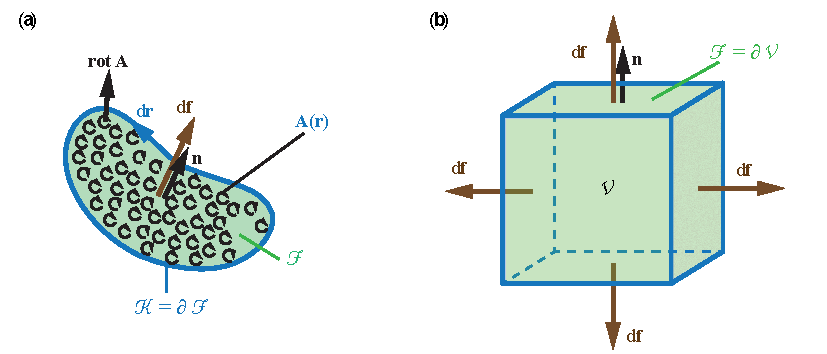
\includegraphics[width=\textwidth]{IntegralsaetzeEdyn.pdf}
  \caption[Orientierte Fl�chen f�r die Integrals�tze.]{Orientierte Fl�chen f�r die Integrals�tze. a) Stokes-Integralsatz. Das Oberfl�chenelement $d\vec{f}$ kann geschrieben werden als: $\D \vec{f} = \vec{n}\, \D f$, worin $ \vec{n}$ der Normalenvektor auf die Fl�che $\mathcal{F}$ ist. b) Gau�-Integralsatz. Auch hier ergibt sich das Oberfl�chenelement durch  $\D \vec{f} = \vec{n}\, \D f$. Wir bezeichnen hier den Volumenbereich mit $\mathcal{V}$, Fl�chen \bzw Oberfl�chen mit $\mathcal{F}$ und Konturen/Linien mit $\mathcal{K}$, das Symbol $\d$ bedeutet in diesem Kontext Berandung, $\d \mathcal{F}$ ist also die Berandung von $\mathcal{F}$ und somit eine Kontur $\mathcal{K}$.}
  \label{abb:kontmech_Integralsaetze}
\end{figure}


\subsubsection{Integralsatz von Stokes} \label{kap:kontmech_Integralsatz_Stokes}

Als erstes geben wir ohne Beweis (wir verweisen auf die Literatur \zb \cite{Otto2019, Fischer2018} und \cite{Schmutzer2005, Bartelmann2015}) den Integralsatz von Stokes an, der auch als Rotationssatz bekannt ist:
\begin{align}
    \int\displaylimits_{\mathcal{F}} \rotv \,\vec{A} \:\D\vec{f} &= \oint\displaylimits_{\mathcal{K} = \d \mathcal{F}} \vec{A}\cdot \D \vec{r} \quad~~\text{\bzw}\quad~~
    \int\displaylimits_{\mathcal{F}} \epsilon_{ijk}\,\d_{j} A_k \:\D f_{i} = \oint\displaylimits_{\mathcal{K} = \d \mathcal{F}} A_k \: \D x_{k} \,. \label{eq:kontmech_Integralsatz_Stokes}
\end{align}
Er besagt, dass ein Fl�chenintegral �ber die Rotation eines Vektorfeldes in ein geschlossenes Kurvenintegral �ber die Tangentialkomponente des Vektorfeldes umgewandelt werden kann. Dies ist hilfreich, da das Kurvenintegral das Vektorfeld allein enth�lt und keine Ableitung desselben und in der Regel einfacher zu berechnen ist als ein Fl�chenintegral.
Der Integralsatz von Stokes\index{Integralsatz von Stokes}\indexp{Stokes, Sir George Gabriel} findet in der Elektrodynamik breite Anwendung.

\subsubsection{Integralsatz von Gau�} \label{kap:kontmech_Integralsatz_Gauss}

Der Integralsatz von Gau�\index{Integralsatz von Gau�}\indexp{Gau�, Johann Carl Friedrich} l�sst sich �ber den Integralsatz von Stokes herleiten. Auch hier verweisen wir auf die Literatur \zb \cite{Otto2019, Fischer2018, Schmutzer2005, Bartelmann2015}: \\

\begin{align}
    \int\displaylimits_{\mathcal{V}} \divv\,\vec{A}\:\D V\,&= \oint\displaylimits_{\mathcal{F} = \d \mathcal{V}} \vec{A}\cdot \D \vec{f}\, \quad~~\text{\bzw}\quad~~
    \int\displaylimits_{\mathcal{V}} \d_{i}\,A_i \:\D V\,= \oint\displaylimits_{\mathcal{F} = \d \mathcal{V}} \,A_i\:\D f_{i} \,.  \label{eq:kontmech_Integralsatz_Gauss}
\end{align}

Mit den Integrals�tzen kann man, ohne weiter auf spezielle Koordinaten zur�ckgreifen zu m�ssen, anschaulich erkl�ren, warum Gradientenfelder wirbelfrei und Wirbelfelder quellenfrei sind. In \probref{kontmech_integralsaetze} berechnen wir die Integrale \eqref{eq:kontmech_Integralsatz_Stokes} und \eqref{eq:kontmech_Integralsatz_Gauss} 
f�r verschiedene Vektorfelder jeweils nach beiden Seiten der Gleichungen.

\subsubsection{Zerlegungssatz f�r Vektorfelder} \label{kap:kontmech_Zerlegungssatz}\index{Zerlegungssatz!Vektorfelder}

Der Zerlegungssatz f�r Vektorfelder lautet: Jedes �berall stetige und im Unendlichen verschwindende Vektorfeld $\vec{A}$ l�sst sich eindeutig als Summe eines wirbelfreien und eines quellenfreien Feldes darstellen:
\begin{align*}
    \vec{A} = \vec{A}^{\lk q\rk}+ \vec{A}^{\lk w\rk} \,,
\end{align*}
worin $\vec{A}^{\lk q\rk}$ das Quellenfeld und $\vec{A}^{\lk w\rk}$ das Wirbelfeld bezeichnen.
Die beiden Feldanteile lassen sich beschreiben durch:\
\begin{align}
    \vec{A}^{\lk q\rk}(\vec{r})&= -\gradv  \lk \frac{1}{4\pi}\int\limits_\mathcal{V} \frac{\divv \vec{A}\lk \vec{r}'\rk}{|\vec{r} - \vec{r}'|}\,\D V'\rk \label{eq:wirbelfeld01} \,, \\
    \vec{A}^{\lk w\rk}(\vec{r})&= +\rotv \lk \frac{1}{4\pi}\int\limits_{\mathcal{F} = \d \mathcal{V}} \frac{\rotv \vec{A}\lk \vec{r}'\rk}{|\vec{r} - \vec{r}'|}\,\D f'\rk \label{eq:wirbelfeld02}
\end{align}
Wir verweisen auf \cite{Schmutzer2005}, wo f�r diese Darstellungen von $\vec{A}^{\lk q\rk}$ \bzw  $\vec{A}^{\lk w\rk}$ nach einer etwas l�ngeren Rechnung folgende Beziehungen bewiesen werden k�nnen:
\begin{align}
    \rotv \vec{A}^{\lk q\rk} = 0\,,\,\divv  \vec{A}^{\lk q\rk} = \divv \vec{A} ~~~~\text{und} ~~~ \divv \vec{A}^{\lk w\rk} = 0 \,,\,\rotv \vec{A}^{\lk w\rk} = \rotv \vec{A}\,. \label{eq:wirbelfeld03}
\end{align}
%Das bedeutet, dass au�er Quellen und Wirbel keine weitere Ursachen f�r eine Wirbelbildung in Frage kommen. \\

Mit diesem Handwerkszeug der Vektoranalysis sind wir nun gut ger�stet, um die Beschreibung der Bewegungsvorg�nge in kontinuierlichen K�rpern in Angriff zu nehmen. 
%\textbf{Green'sche Integrals�tze:
%\begin{align}
    %\int\displaylimits_{\text{V}}\D V \lek\lk\vec{\nabla} \phi \rk\lk \nablav \chi\rk + \phi\,\Delta\chi\rek &=  \oint\displaylimits_{\d V}\D \vec{A}\,\phi\,\vec{\nabla}\chi ~~~\text{\bzw}\\
    %\int\displaylimits_{\text{V}}\D V\,\lk\phi\,\Delta\chi-\chi\,\Delta\phi\rk &= \oint\displaylimits_{\d V} \D \vec{A}\,\lk\phi\,\vec{\nabla}a\chi-\chi\,\vec{\nabla}\phi\rk\,.
%\end{align}

\clearpage
\section{Kinematik und Dynamik kontinuierlicher K�rper}
\label{kap:kontmech_kindyn}

\subsection{Materiepunkte und Koordinaten}
\label{kap:kontmech_materiepunkte} \index{Koordinaten!kontinuierliche K�rper}

Um Bewegungen kontinuierlicher K�rper beschreiben zu k�nnen, ben�tigen wir
zun�chst Koordinaten, in denen wir sie beschreiben k�nnen. Anders als beim
starren K�rper ist es nun bei Fluiden nicht mehr sinnvoll, ein unver�nderliches
k�rperfestes Koordinatensystem einzuf�hren, da sich der K�rper (das Fluid) selbst
mit der Zeit �ndern kann und sich einzelne Teile des Fluids gegeneinander
bewegen k�nnen. Sie w�ren also auch in einem k�rperfesten System nicht mehr
unver�nderlich. Zur Beschreibung greift man einzelne Materiepunkte wie den
Punkt~$\vec{\hat{P}}$ in \figref{kontmech_KontKoerpKoord01} heraus und
betrachtet das infinitesimale Volumen $V$ um diese herum.

\begin{figure}
  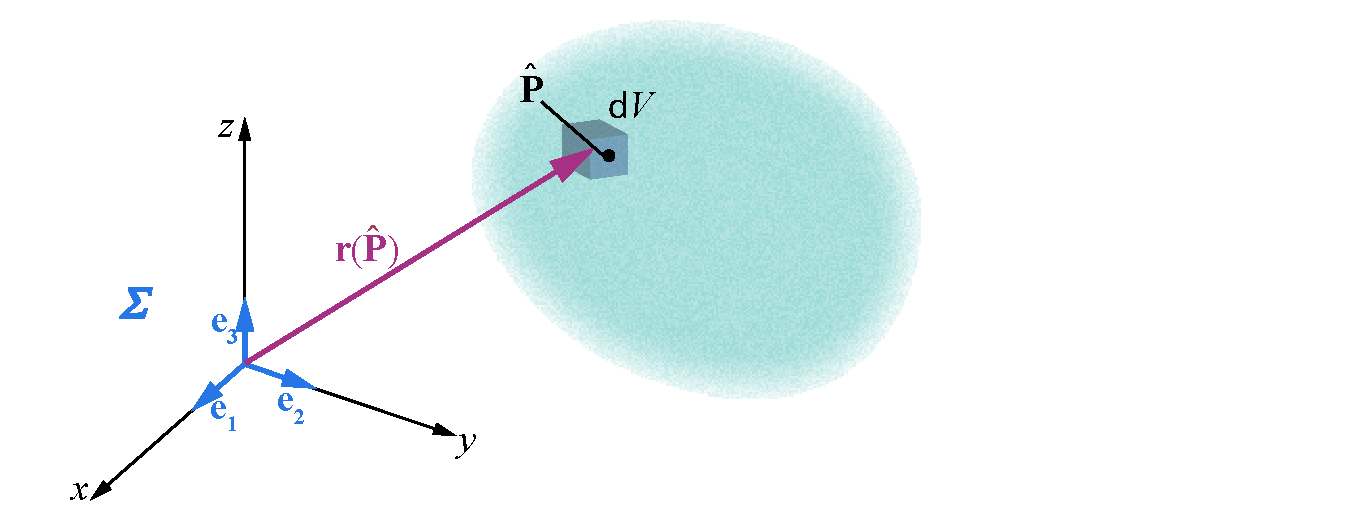
\includegraphics[width=\textwidth]{KontKoerpKoord.pdf}
  \caption[Materiepunkt und Raumpunkt eines kontinuierliechen K�rpers]{In der
    Beschreibung eines kontinuierlichen K�rpers ordnet man jedem Materiepunkt
    $\hat{\vec{P}}$ des K�rpers einen Raumpunkt $\vec{r}$ zu.}
    \label{abb:kontmech_KontKoerpKoord01}
\end{figure}

Der K�rper ist dann durch die Ansammlung eines Kontinuums von Materiepunkten
$\vec{\hat{P}}$ und die darin enthaltene Masse $\D m(\vec{\hat{P}})
= \varrho(\vec{\hat{P}})\,\mathrm{d}V$ beschrieben. Die Beschreibung erfolge in
einem raumfesten Koordinatensystem \vec{\Sigma}. Die zugeh�rigen Vektoren
nennen wir, wie wir es aus den vorherigen Kapiteln gewohnt sind, $\vec{r}
= \sum x_i\, \vec{e}_i\,, i=1 \ldots 3 $. Die Punkte $\vec{\hat{P}}$ kann man
dadurch festlegen, dass man ihnen Koordinaten in $\vec{\Sigma}$ zu einem festen
Zeitpunkt $t_0$ zuordnet,
\begin{equation}
  \vec{\hat{P}} \Leftrightarrow \vec{r}(\vec{\hat{P}},t_0) \; .
  \label{eq:kontmech_Materiepunkt}
\end{equation}

Damit bieten sich zwei M�glichkeiten, den
kontinuierlichen K�rper zu beschreiben. Wir k�nnen einerseits angeben,
an welchen Orten $\vec{r}$ sich die Materiepunkte $\vec{\hat{P}}$ in $\vec{\Sigma}$ 
befinden\footnote{Wir bezeichnen somit die Koordinaten eines Punktes
  $\vec{\hat{P}}$ mit dem Vektor $\vec{r}(\vec{\hat{P}})$. $\vec{\hat{P}}$ ist
  nicht zu verwechseln mit dem sp�ter eingef�hrten Druck $p$ im Fluid.}
\begin{subequations}
  \begin{equation}
    \vec{r} = \vec{r}(\vec{\hat{P}},t) \,.
    \label{eq:kontmech_EulerKoord}
  \end{equation}
  Dies nennt man in der Kontinuumsmechanik \gls{eulerscheKoordinaten}\index{Euler-Koordinaten}\indexp{Euler, Leonhard}. Bei der Eulerschen Beschreibung bleibt das \KOS quasi ortsfest. Wenn man eine physikalische Gr��e wie \zb die Geschwindigkeit $\vec{v}$ an einem Ort $\vec{r}$ zur Zeit $t$ betrachtet, so beschreibt diese Gr��e zu verschiedenen Zeiten verschiedene Fluidelemente $\vec{\hat{P}}_i$.\\
	Andererseits kann man einen kontinuierlichen K�rper auch dadurch beschreiben, dass
  man angibt, welcher materielle Punkt $\vec{\hat{P}}$ sich zu einer Zeit $t$
  am Ort $\vec{r}$ befindet,
  \begin{equation}
    \vec{\hat{P}} = \vec{\hat{P}}(\vec{r},t) \; .
    \label{eq:kontmech_LagrangeKoord}
  \end{equation}
  Dies sind \gls{lagrangescheKoordinaten}\index{Lagrange-Koordinaten}\indexp{Lagrange, Joseph-Louis}. Diese werden dadurch erm�glicht,
  dass niemals zwei materielle Punkte sich am selben Ort befinden k�nnen.
  Dadurch wird Gleichung \eqref{eq:kontmech_EulerKoord} umkehrbar und
  \eqref{eq:kontmech_LagrangeKoord} kann immer angegeben werden. Bei einer Beschreibung nach Lagrange wird das \KOS quasi mit den Materiepunkten mitbewegt, in der Beziehung \eqref{eq:kontmech_LagrangeKoord} beziehen wir uns immer auf das gleiche Fluidelement $\hat{\vec{P}}$.
\end{subequations}

\subsection{Kinematik}
\label{kap:kontmech_kinematik} \index{Kinematik!kontinuierliche K�rper}

\subsubsection{Geschwindigkeiten und Str�mungen}
\label{kap:kontmech_Geschwindigkeit} \index{Geschwindigkeit!kontinuierliche K�rper} \index{Str�mung}

Wir wollen nun im Sinne der Newtonschen Mechanik die Bewegung der Materiepunkte des Fluids betrachten. Die Geschwindigkeit eines Materiepunktes ist, da dieser nach
\eqref{eq:kontmech_Materiepunkt} selbst in der Zeit unver�nderlich ist, nur
von der �nderung seiner Position abh�ngig,
\begin{subequations}
  \begin{equation}
    \vec{v}(\vec{\hat{P}} ,t) = \frac{\D}{\D t} \vec{r}(\hat{\vec{P}},t) = \frac{\partial}
    {\partial t}\vec{r}(\vec{\hat{P}} ,t) \; . \label{eq:kontmech_GeschwZeit}
  \end{equation}
  Dies stellt die Geschwindigkeit dar, die ein Materiepunkt zum Zeitpunkt $t$
  hat. Dieser Materiepunkt �ndert dabei nat�rlich seinen Ort mit der Zeit.
  M�chte man die Geschwindigkeit wissen, die ein beliebiger Materiepunkt zum
  Zeitpunkt $t$ an einem bestimmten Ort $\vec{r}$ hat, muss man die
  Lagrangekoordinate \eqref{eq:kontmech_LagrangeKoord} in die Beziehung \eqref{eq:kontmech_GeschwZeit} f�r die Geschwindigkeit
  einsetzen und man erh�lt
  \begin{equation}
    \vec{v}(\vec{r},t) = \vec{v}(\vec{\hat{P}}(\vec{r},t),t) \; .
    \label{eq:kontmech_GeschwOrt}
  \end{equation}
\end{subequations}

Bei dieser Betrachtung wird gleich deutlich, dass man mit einer Geschwindigkeit
in einer Fl�ssigkeit oder einem Gas verschiedene physikalische Sichtweisen
meinen kann. Die gesamte Bewegung des Fluids zu einem Zeitpunkt $t$ nennt man \textit{Str�mung}\index{Str�mung}. Diese Str�mung l�sst sich
entsprechend auch auf verschiedene Arten beschreiben. Ein Spezialfall ist eine
\emph{station�re Str�mung}, die in der Zeit konstant ist, f�r die also gilt 
$\vec{v}(\vec{r},t) = \vec{v}(\vec{r})$.

Die Ortskurve, die ein bestimmter Materiepunkt in der Zeit durchl�uft, nennt
man eine \gls{Bahnlinie}\index{Bahnlinie}. Ist das Geschwindigkeitsfeld
\eqref{eq:kontmech_GeschwOrt} bekannt, erh�lt man die Bahnlinie durch
Integration von diesem Geschwindigkeitsfeld $\vec{v}(\vec{r},t)$ �ber die Zeit.

Die Linie, die immer tangential an das Geschwindigkeitsfeld zu einem festen
Zeitpunkt~$t$ anliegt, nennt man eine \gls{Stromlinie}\index{Stromlinie}.
Diese Stromlinien stellen dar, wie die Str�mung zum aktuellen Zeitpunkt $t$ 
verl�uft. In jedem Raumpunkt befindet sich dabei ein anderer Materiepunkt und
hat aktuell diese Geschwindigkeit $\vec{v}(\vec{r},t)$. Dies muss nicht mit der Bahnkurve
�bereinstimmen, siehe \figref{kontmech_KontKoerpKoord02}. In einer station�ren
Str�mung werden jedoch beide Linien �bereinstimmen.

\begin{figure}
  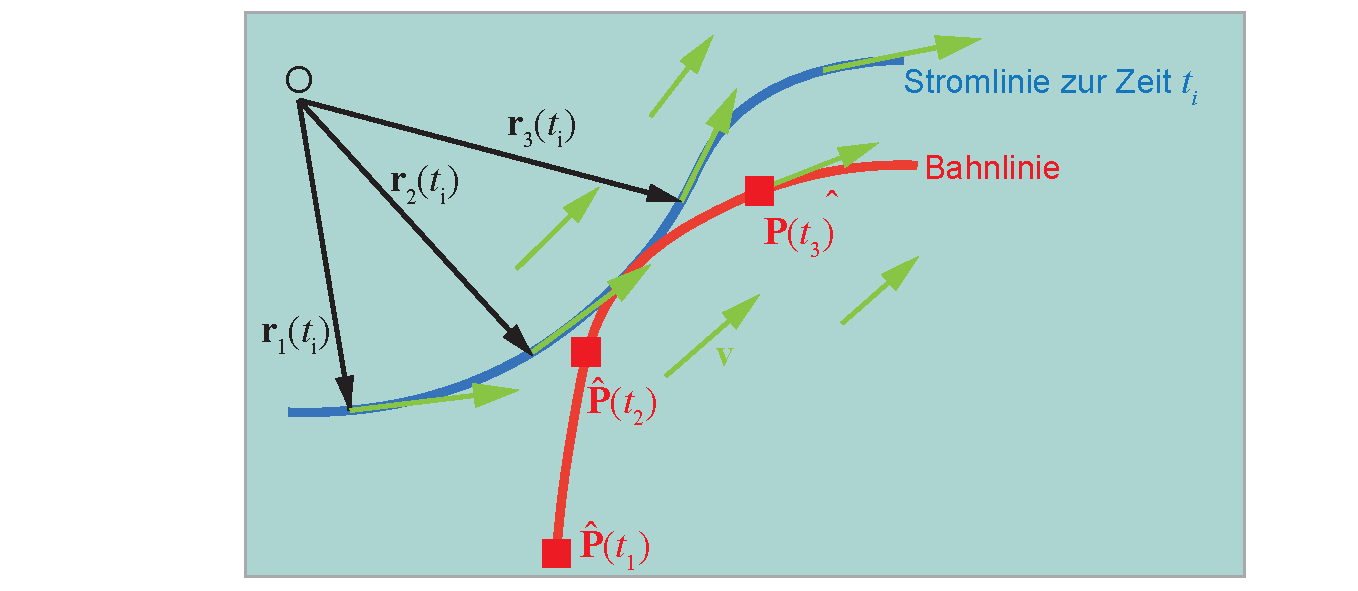
\includegraphics[width=\textwidth]{KontStromlinie.pdf}
  \caption[Bahn- und Stromlinie einer Str�mung]{Eine \gls{Stromlinie} (blau)
    liegt tangential am Geschwindigkeitsfeld zu einem festen Zeitpunkt (gr�ne
    Pfeile) an. Im Gegensatz dazu beschreibt eine \gls{Bahnlinie} (rot) die
    Ortskurve, die ein Materiepunkt mit der Zeit durchl�uft.}
    \label{abb:kontmech_KontKoerpKoord02}
\end{figure}

Str�mungen werden sehr stark von inneren Reibungen beeinflusst. Das trifft
besonders stark auf Fl�ssigkeiten zu. Weil die Reibung, die wir mit der sp�ter 
zu definierenden Viskosit�t\index{Viskosit�t} bezeichnen wollen (siehe \kap{kontmech_InnereReibung}),  dabei das Verhalten
der str�menden Fl�ssigkeit in der Art der Str�mung sehr stark beeinflussen
kann, unterscheidet man je nach St�rke der Reibung die Art der Str�mung.
Eine \emph{ideale Fl�ssigkeit}\index{Fl�ssigkeit!ideale} wird dabei kaum von
der Reibung beeinflusst.
Sie ist dadurch gekennzeichnet, dass die Reibungskr�fte klein gegen alle
anderen an der Fl�ssigkeit angreifenden Kr�fte sind. Dieses Verhalten trifft
meist auch auf Gase zu.  Im Gegensatz dazu ist eine \emph{stark viskose
  Fl�ssigkeit} eine, in der die Reibungskr�fte dominieren. Die meisten
\emph{realen Fl�ssigkeiten} befinden sich im Bereich dazwischen.

Eine Str�mung wird als \emph{laminar}\index{Str�mung!laminar} bezeichnet,
wenn \gls{Bahnlinie}n benachbarter
Materiepunkte nebeneinander liegen, ohne sich zu durchmischen. Viskose
Fl�ssigkeiten tendieren zu einem laminaren Str�mungsverhalten, weil hier die
Reibungskr�fte gegen�ber den beschleunigenden Kr�ften dominieren. Ist die
Reibung klein gegen die beschleunigenden Kr�fte, kann das Str�mungsbild unruhig
werden. Das geschieht insbesondere dann, wenn die Fl�ssigkeit an ihren
Grenzen (\zb dem Rand eines Rohres) durch st�rkere Reibungskr�fte an diesem
Rand beeinflusst wird. In diesem Fall kann die Str�mung
\emph{turbulent}\index{Str�mung!turbulent} werden (siehe auch �bersicht \ref{tab:kontmech_stroemung_overview}).


\subsubsection{Beschleunigungen}
\label{kap:kontmech_Beschleunigung} \index{Beschleunigung!kontinuierliche K�rper}

Als \emph{materielle}\index{Beschleunigung!materielle} oder
\emph{substantielle Beschleunigung}\index{Beschleunigung!substantielle}
definieren wir die Beschleunigung, die ein Materieteilchen am Ort $\vec{r}$
erf�hrt,\dh in dem wir \eqref{eq:kontmech_GeschwOrt} ableiten:
\begin{align}
\begin{split}
  \vec{a}(\vec{r},t) &= \frac{\D}{\D t} \vec{v}(\vec{r},t) = \dot{\vec{v}}(\vec{r},t)
  = \sum_{i=1}^3 \frac{\partial \vec{v}(r,t)}{\partial x_i} \frac{\D x_i}{\D t} \,\vec{e}_i
  + \frac{\partial}{\partial t} \vec{v}(\vec{r},t) \\
  &= \lk \vec{v}(\vec{r},t) \cdot \nablav \rk \vec{v}(\vec{r},t)
  + \frac{\partial}{\partial t} \vec{v}(\vec{r},t) \; . 
\end{split} \label{eq:kontmech_Beschleunigung}
\end{align}
Man erkennt hier die Dyade $\cdot \nablav$ \eqref{eq:kontmech_nablaop03} wieder und dass es zwei Beitr�ge zur �nderung der Geschwindigkeit gibt.
Einerseits kann sich das Geschwindigkeitsfeld mit der Zeit selbst �ndern.
Dies wird durch die partielle Ableitung im zweiten Term beschrieben. Der
erste Term ber�cksichtigt, dass sich der Materiepunkt an einen anderen
Raumpunkt bewegt und somit auch der r�umlichen �nderung des
Geschwindigkeitsfeldes unterliegt. Diesen Teil der Beschleunigung nennt man
\emph{Konvektionsbeschleunigung}\index{Konvektionsbeschleunigung}\index{Beschleunigung!Konvektions-}. 
Man erkennt an \eqref{eq:kontmech_Beschleunigung} wieder, 
dass wir bei der Beschreibung von Kinematik und Dynamik des Kontinuums auf partielle Differentialgleichungen 
treffen.

\subsection{Eigenschaften von Str�mungen}
\label{kap:kontmech_EigenschaftenStroemungen} 
\subsubsection{Stromdichte, Fluss und Kontinuit�tsgleichung}
\label{kap:kontmech_Stromdichte}\index{Kontinuit�tsgleichung!kontinuierliche K�rper}

Bei der Betrachtung von Str�mungen interessiert man sich oft daf�r, wie
sich die Materie, die eine Dichte $\varrho$ haben soll, bewegt. Dazu f�hren wir die \emph{Stromdichte}\index{Stromdichte}
\begin{equation}
  \vec{j} = \varrho \,\vec{v}
  \label{eq:kontmech_Stromdichte}
\end{equation}
ein, die nicht nur die Geschwindigkeit beschreibt, sondern beschreibt, wie
sich die Materie mit dieser Geschwindigkeit bewegt. In einem differentiellen
Volumenelement erhalten wir
\begin{equation*}
  \vec{j}\,\D V = \varrho\,\D V\,\vec{v} = \D m \, \vec{v} \; .
\end{equation*}
Die Stromdichte tritt also f�r das kontinuierliche System an die Stelle
des Impulses und hat die Einheit einer Impulsdichte ($\SI{}{\kg\per\metre\squared\per\second}$).

Der \emph{Fluss}\index{Fluss} einer Str�mung durch eine Oberfl�che l�sst sich durch
\begin{equation*}
  \Phi = \int_A \vec{j} \cdot \D\vec{A} = \int_A \varrho \,\vec{v} \cdot
  \D\vec{A}
\end{equation*}
berechnen und gibt an, wie viel der Materie in einer gewissen Zeit durch
die Querschnittsfl�che $A$ flie�t.

Der Fluss ist ebenfalls entscheidend, wenn wir die Masse in einem
bestimmten, zeitlich konstanten Volumenelement betrachten m�chten. Diese
k�nnen wir jederzeit durch das Integral
\begin{equation*}
  m = \int_V \varrho\,\D V
\end{equation*}
berechnen. Die Massenerhaltung verlangt, dass die zeitliche �nderung
der Masse im Volumen gerade der Masse entspricht, die zu- bzw. abflie�t.
Man kann also die Erhaltungsgleichung
\begin{equation*}
  \frac{\partial}{\partial t} M = \int_V \frac{\partial}{\partial t}\varrho\,\D V 
  = -\int_{A = \partial V} \vec{j}\cdot \D\vec{A} = \Phi 
\end{equation*}
aufstellen, wobei das Oberfl�chenintegral gerade �ber den gesamten Rand
des Volumens~$V$ geht, den wir mit $\partial V$ bezeichnen wollen, $\Phi$ ist der Materiefluss in $\SI{}{\kg\per\second}$. Das Minus\-zeichen r�hrt daher, dass die Randfl�che
nach au�en orientiert ist. Das Skalarprodukt $\vec{j}\cdot \D\vec{A}$
liefert also dann einen positiven Wert, wenn es einen Netto-Abfluss von
Masse gibt. Mit dem Integralsatz von Gau� \eqref{eq:kontmech_Integralsatz_Gauss} l�sst sich das Oberfl�chenintegral
umformen, so dass wir 
\begin{equation}
  \int_V \frac{\partial}{\partial t}\varrho\,\D V 
  = -\int_V \divv \vec{j}\, \D V
  \label{eq:kontmech_KontinuitaetsglMakr}
\end{equation}
erhalten.

Gleichung \eqref{eq:kontmech_KontinuitaetsglMakr} muss f�r jedes beliebige
Volumen gelten. Wir haben nur vorausgesetzt, dass dieses zeitlich konstant sein
soll. Damit l�sst sich dann die differentielle Form der
\emph{Kontinuit�tsgleichung}\index{Kontinuit�tsgleichung}
\begin{equation}
  \frac{\partial}{\partial t}\varrho + \divv \vec{j} =
  \frac{\partial}{\partial t}\varrho + \divv \lk \varrho\, \vec{v} \rk = 0
  \label{eq:kontmech_KontinuitaetsglDiff}
\end{equation}
aufstellen.

Ein interessanter Spezialfall sind \emph{inkompressible} Fl�ssigkeiten\index{Fl�ssigkeit!inkompressible}.
Diese zeichnen sich dadurch aus, dass ihre Dichte zeitlich und r�umlich
konstant ist. Das hei�t $\partial \varrho/ \partial t = 0$ und $\divv\lk
\varrho\, \vec{u} \rk = \varrho \divv \vec{u}$. Im Fall imkompressibler Fluide vereinfacht sich
die Kontinuit�tsgleichung zu
\begin{equation}
  \divv \vec{v}  = 0 \; .
  \label{eq:kontmech_KontinuitaetsglInkompr}
\end{equation}
Das Str�mungsfeld weist also keine Divergenzterme auf. Dies entspricht der
Tatsache, dass an keinem Punkt in der inkompressiblen Fl�ssigkeit Masse
konzentriert oder ausged�nnt werden kann. 

\subsubsection{Formen von Str�mungen}
\label{kap:kontmech_FormenStroemungen}\index{Str�mung!Formen}

Str�mungen k�nnen sehr unterschiedliche Formen annehmen. Wir wollen vor
allem laminare und turbulente Str�mungen unterscheiden.

\index{Str�mung!laminar|textbf}%
Als \emph{laminar} bezeichnen wir Str�mungen, bei denen verschiedene
Schichten der Fl�ssigkeit oder des Gases sich nicht miteinander mischen. Das hei�t
nicht, dass sie sich alle identisch bewegen m�ssen. Sie k�nnen \zb
unterschiedliche Geschwindigkeiten haben, gleiten dann aber glatt aneinander
vorbei. Beispiele sind in \figref{kontmech_FormenStroemungen}a gezeigt.
Laminare Str�mungen treten immer dann auf, wenn der Energie�bertrag innerhalb
der Fl�ssigkeit oder des Gases gro� ist, also die interne Reibung eine gro�e
Rolle spielt und damit die Bewegung des Kontinuums dominiert. 

\begin{figure}
  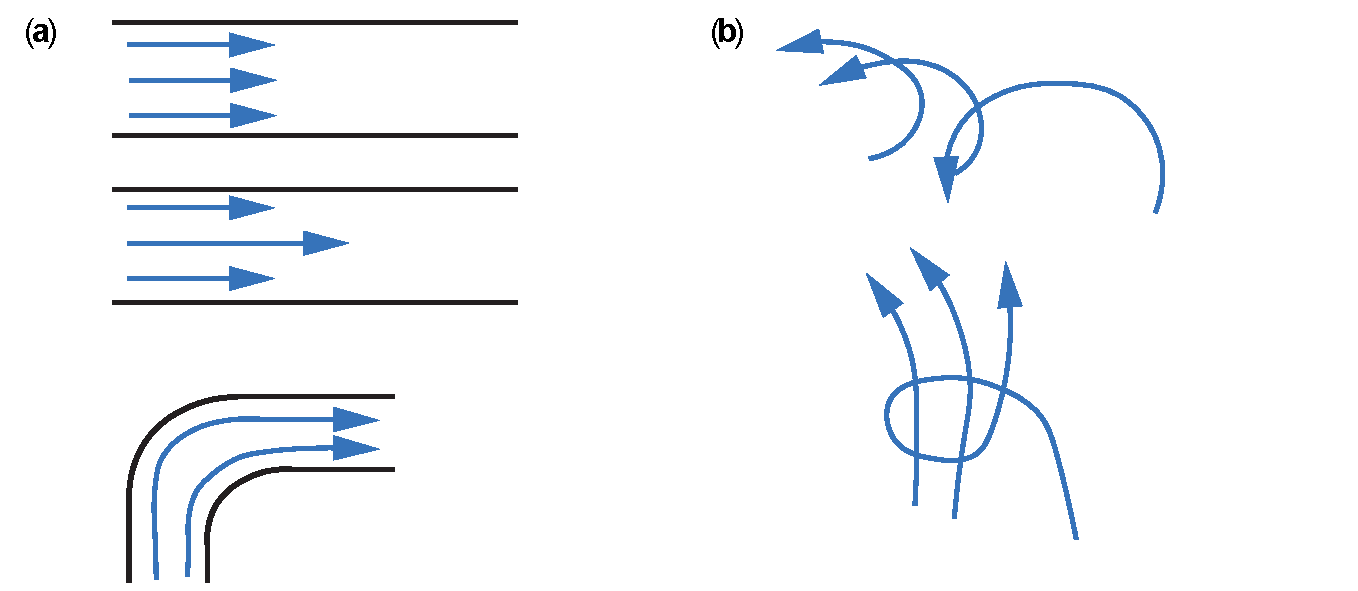
\includegraphics[width=\textwidth]{FormenStroemungen.pdf}
  \caption[Formen von Str�mungen]{Formen von Str�mungen. \fa In laminaren
    Str�mungen gleiten unterschiedliche Schichten glatt, \dh ohne Vermischung, aneinander vorbei.
    \fb In turbulenten Str�mungen schneiden sich die \gls{Bahnlinie}n der
    einzelnen Schichten. Es kommt zu Durchmischungen der Schichten.}
  \label{abb:kontmech_FormenStroemungen}
\end{figure}

\index{Str�mung!turbulent|textbf}%
Sobald dies nicht mehr erf�llt ist, k�nnen die verschiedenen Schichten leicht
ineinander eindringen, verwirbeln  und miteinander mischen. Solche Str�mungen
nennen wir \emph{turbulent}. Beispiele daf�r sind in
\figref{kontmech_FormenStroemungen}b gegeben.
  
Ein weiteres wesentliches Charakteristikum von Str�mungen ist ihre \emph{Rotation}\index{Str�mung!Rotation}\index{Rotation!Str�mung}.
Rechnerisch ergibt sich diese aus der Geschwindigkeit durch $\rotv \vec{v}$.
Sie gibt an, ob sich Objekte, die sich in der Str�mung bewegen, in
eine Rotationsbewegung versetzen lassen. Das ist sehr offensichtlich
bei vorhandenen Wirbeln der Fall. Tats�chlich sind aber auch rein gerade
Str�mungen nicht rotationsfrei. Im Beispiel nach \figref{kontmech_Rotation} sieht man, 
dass sich in einer gerade verlaufenden Str�mung mit in einer Dimension unterschiedlichen
Geschwindigkeiten ein Objekt drehen wird. Der zun�chst mit seiner langen Seite
senkrecht zur Str�mung ausgerichtete Balken wird an seinen beiden Enden
unterschiedlich schnell bewegt. F�r gr��ere Zeiten sieht man, wie sich das zu
einer Rotation ausbildet, die mit der Translationsbewegung des
Massenmittelpunkts in Str�mungsrichtung �berlagert ist.

\begin{figure}
  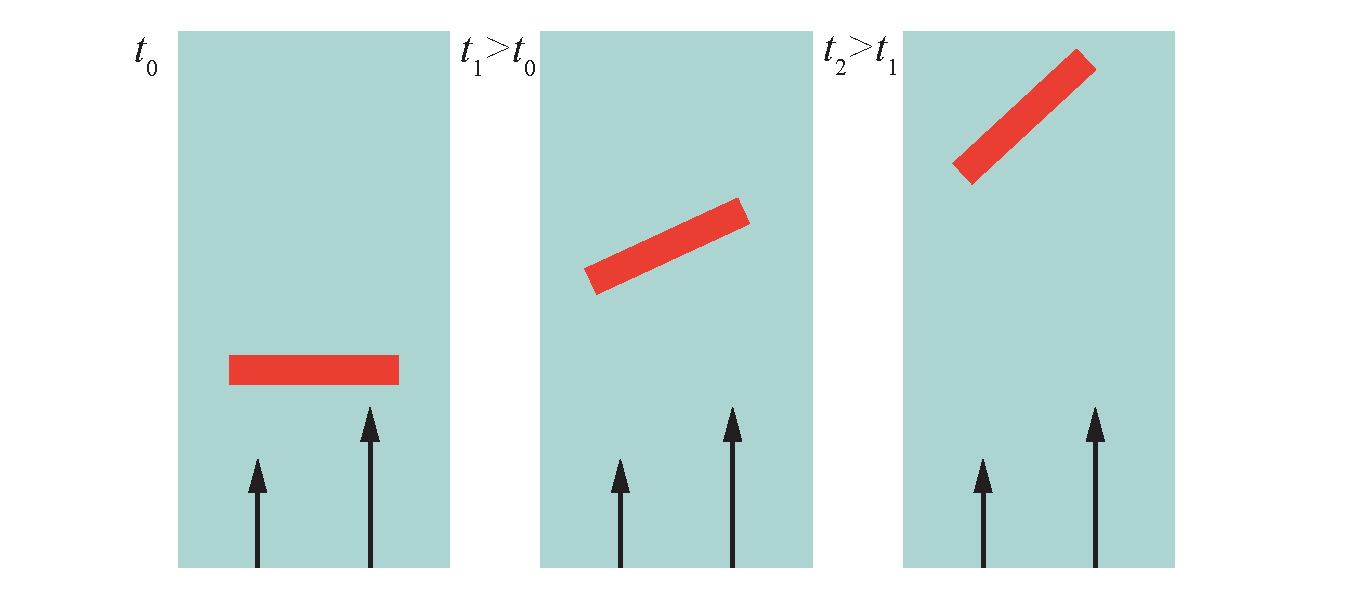
\includegraphics[width=\textwidth]{StroemungRotation.pdf}
  \caption[Nichtverschwindende Rotation in einer gerade Str�mung]
  {Nichtverschwindende Rotation in einer gerade in $z$-Richtung verlaufenden Str�mung mit unterschiedlichen
    Geschwindigkeiten in den einzelnen Schichten entlang $x$-Richtung.}
  \label{abb:kontmech_Rotation}
\end{figure}

Ein besonderer Fall der Str�mung eines Fluids ist die \emph{Potentialstr�mung}\index{Potentialstr�mung}, bei der das Geschwindigkeitsfeld $\vec{v}(\vec{r})$ ein Potential besitzt. Ein solches Potential ist in einem homogenen Fluid vorhanden, wenn die Str�mung wirbelfrei und die inneren Reibungskr�fte vernachl�ssigbar klein sind. Potentialstr�mungen k�nnen sehr vorteilhaft mit mathematischen Methoden der Potentialtheorie behandelt werden, wir verweisen hierzu auf die weiterf�hrende Literatur \cite{Schmutzer2005, Altenbach2018, Rannacher2017}.

\subsection{Dynamik kontinuierlicher K�rper}\label{kap:kontmech_dynamik}
\index{Dynamik!kontinuierliche K�rper}

\subsubsection{Euler-Gleichung}\indexp{Euler, Leonhard}
\label{kap:kontmech_EulerGl}\index{Euler-Gleichung (Kontinuumsmechanik)|textbf}

Auf eine Fl�ssigkeit oder ein Gas k�nnen mehrere Formen von Kr�ften angreifen.
Diese verursachen, wie es in Erweiterung der Newtonschen Bewegungsgleichungen
\eqref{eq:bew_NewtonBGL} sein muss, eine Beschleunigung des Volumenelements
$\D V$ aus \figref{kontmech_KontKoerpKoord02}. F�r dieses differentielle
Volumenelement formulieren wir unter Benutzung von \eqref{eq:kontmech_Beschleunigung} die Newtonschen Bewegungsgleichungen in
der Form
\begin{equation}
  \varrho\, \D V\, \vec{a}(\vec{r},t) = \sum_i \vec{F}_i  \label{eq:kontmech_kraefte_an_dV}
\end{equation}
mit der Summe aller am Volumenelement $\D V$ angreifenden Kr�fte. Dabei werden wir
drei Formen von Kr�ften unterscheiden:

\begin{enumerate}
\item Auf das Fluid wirken externe 
  \emph{Volumenkr�fte}\index{Volumenkr�fte}, die
  an jedem Raumpunkt direkt angreifen (wie \zb die Schwerkraft). Diese Kr�fte wollen wir mit
  \begin{equation*}
    \vec{F}_\text{V} = \vec{f}_\text{V} \D V
  \end{equation*}
  bezeichnen, wobei $\vec{f}_V$ die Kraftdichte darstellt.
\item Die Volumenelemente �ben �ber ihre Grenzfl�chen eine Kraft auf die benachbarten Elemente aus. Diese Kr�fte definieren den Druck $p(\vec{r}')$ an der Stelle $\vec{r}'$ auf ein Volumenelement $\D V$. Ist
  dieser Druck nicht homogen, resultiert eine Kraft auf das Volumen, die sich durch
  das Oberfl�chenintegral
  \begin{equation*}
    \vec{F}_\text{D} = -\int_{\partial V} p(\vec{r}')\, \D \vec{A}'
  \end{equation*}
  �ber den Rand $\partial V$ von $\D V$ berechnen l�sst, wobei das
  Fl�chenelement nach au�en orientiert ist. Das differentielle Volumenelement
  wollen wir durch einen W�rfel der Kantenl�nge $\Delta l$ beschreiben. Der
  Materiepunkt, auf den die Kraft wirkt, liege in der Mitte des W�rfels.
\begin{figure}
  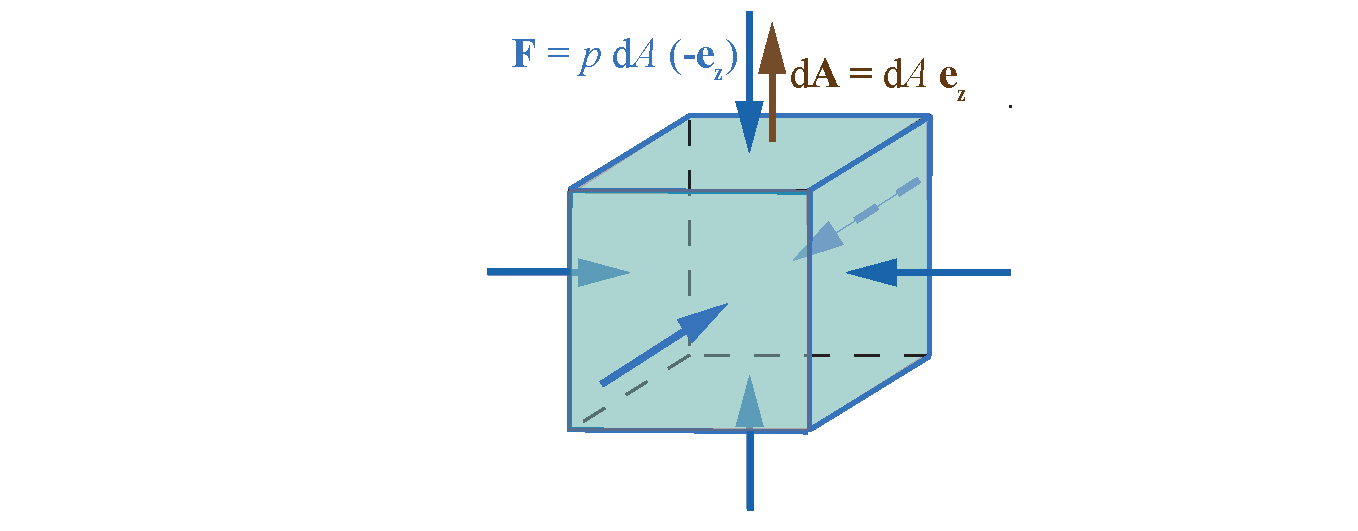
\includegraphics[width=\textwidth]{KontDruck.pdf}
  \caption[Druck auf das Volumenelement einer Fl�ssigkeit]{Druck auf das
    Volumenelement einer Fl�ssigkeit. Das Volumenelement wird durch einen
    W�rfel approximiert. Die Kr�fte wirken entgegen der nach au�en orientierten
    Normalenvektoren auf die Fl�che.}
  \label{abb:kontmech_KraefteDruck}
\end{figure}
  Dann wird das Integral (vgl. \figref{kontmech_KraefteDruck}) zu 
  \begin{align*}
    - \int_{\partial V} p(\vec{r}')\, \D \vec{A}'
    = &-p(x-\Delta l/2,y,z) \, \D A \, \lk -\veceX \rk - p(x+\Delta l/2,y,z)
        \, \D A \, \veceX \\
      &- p(x,y-\Delta l/2,z) \, \D A \, \lk -\veceY \rk  - p(x,y+\Delta l/2,z)
        \, \D A \, \veceY \\
      &- p(x,y,z-\Delta l/2) \, \D A \, \lk -\veceZ \rk  - p(x,y,z+\Delta l/2)
        \, \D A \, \veceZ \; .
  \end{align*}
  Ber�cksichtigen wir, dass im differentiellen Volumenelement eine
  Linearisierung des Drucks im Volumen ausreicht, so l�sst sich dies
  umschreiben zu
  \begin{equation*}
    \vec{F}_\text{D} = -\frac{\partial p(\vec{r})}{\partial x} \, \Delta l\, \D A \,\veceX 
		                   - \frac{\partial p(\vec{r})}{\partial y} \, \Delta l \, \D A \, \veceY 
											 - \frac{\partial p(\vec{r})}{\partial z} \, \Delta l \, \D A\, \veceZ \;  .
  \end{equation*}
Letztendlich erhalten wir also:
  \begin{equation}
    \vec{F}_\mathrm{D} = -\vec{\nabla} p\, \D V \;  .
    \label{eq:kontmech_Druckkraft}
  \end{equation}
	Wir haben hier bei der Ableitung vorausgesetzt, dass der
Druck jeweils senkrecht auf die Seitenfl�che des betrachteten differentiellen Volumenelements (W�rfel der Kantenl�nge $l$) wirkt.
Bei Fl�ssigkeiten ist das im Allgemeinen erf�llt, bei Festk�rperkontinua muss das nicht der Fall sein. Dann muss man den Gradienten des Drucks (einen Vektor) durch den sogenannten \textit{Spannungstensor} $\sigma$\index{Spannungstensor} ersetzen. Umgekehrt kann man sagen, dass f�r einen Spannungstensor, dessen Nichtdiagonalelemente alle 0 sind, die Diagonalelemente gerade den Gradienten des Drucks darstellen. Wir verweisen dazu auch \kap{kontmech_festelastisch}.
\item Es wirken Reibungskr�fte, die wir zun�chst ganz allgemein mit $\vec{F}_\text{R} = \vec{f}_\text{R}
  \D V$ bezeichnen wollen und sp�ter zwischen inneren Reibungen und Reibungen
  mit dem Rand unterscheiden werden. 
\end{enumerate}
In Summe erhalten wir also f�r \eqref{eq:kontmech_kraefte_an_dV} die
Bewegungsgleichung eines Materiepunkts in der Euler-Betrachtung im Kontinuum 
die \emph{Euler-Gleichung}\index{Euler-Gleichung (Kontinuumsmechanik)}
\begin{equation}
  \varrho \lk \lk \vec{v} \cdot \nabla \rk \vec{v} + \frac{\partial}{\partial t}
  \vec{v} \rk = \vec{f}_\text{V}  + \vec{f}_\text{R} - \vec{\nabla} p \; .
  \label{eq:kontmech_EulerGleichung}
\end{equation}

% BEISPIEL %%%%%%%%%%%%%%%%%%%%%%%%%%%%%%%%%%%%%%%%%%%%%%%%%%%%%%%%%%%%%%%%%%%%%%%%%%%%%%%%%%
\begin{example}{Wasserwellen}\index{Wasserwellen}
\label{bsp:kontmech_Wasserwellen}
Wir werden in \kap{kontmech_festLagrange} die Physik der Wellen, wie sie
in einem kontinuierlichen Medium entstehen, genauer untersuchen. Hier wollen
schon an einem ersten Beispiel zeigen, wie wir aus der Euler-Gleichung
\eqref{eq:kontmech_EulerGleichung} das Auftreten von Wasserwellen und deren
Wellenl�ngenabh�ngigkeit von der Wasserh�he absch�tzen k�nnen.\\
Wasserwellen sind Oberfl�chenwellen an der Grenzfl�che zwischen Wasser und Luft und haben Periodendauern von Sekunden bis mehrere Stunden (siehe Gezeitenwelle\index{Welle!Gezeiten-} \kap{bew_gezeiten}).
Wichtig f�r unsere Betrachtung ist, dass die Wasserteilchen nur relativ kleine Bewegungen ausf�hren, ihre Bewegungsenergie aber an benachbarte Teilchen weiter gibt.
Bei Wellenl�ngen kleiner als $\SI{1}{\centi\metre}$  bestimmen Oberfl�chenspannung und Z�higkeit des Wassers die Eigenschaften der Wellen, bei Wellenl�ngen gr��er als $\SI{10}{\centi\metre}$ ist die Erdanziehungskraft entscheiden, die Wasserwellen sind dann sogenannte Schwerewellen\index{Welle!Schwere-}.
Wasserwellen weichen in ihrer Gestalt von der �blichen Sinusform ab. Der Teil der Welle, der oberhalb des Ruhewasserspiegels ($z=0$) liegt, wird als Wellenberg bezeichnet, die h�chste Auslenkung als Wellenkamm. Der Teil unterhalb des Ruhewasserspiegels hei�t Wellental. Die Wellenh�he ist die Summe der Betr�ge der Maximalauslenkungen von Wellenberg und Wellental. Als Wellenl�nge $\lambda$ wird der Abstand zweier Wellenk�mme bezeichnet (\figref{kontmech_Wasserwellen}).

Wir wollen nun zeigen, wie wir aus der
Euler-Gleichung \eqref{eq:kontmech_EulerGleichung} mit der Gewichtskraft
als Volumenkraft,
\begin{equation}
  \vec{f}_\text{V} = - \varrho g \veceZ \; ,
\end{equation}
eine relevante Aussage f�r die Ausbreitung von Wasserwellen
in Abh�ngigkeit von der Wassertiefe erhalten k�nnen. Dazu arbeiten wir mit dem
Modell nach  \figref{kontmech_Wasserwellen} \cite{Mai2004}. Nach diesem Modell
bewegen sich  die Wassermolek�le nur in der $x$-$z$-Ebene und es k�nnen auch
nur in dieser Ebene  Druck�nderungen auftreten. Die $y$-Richtung wird als
unendlich ausgedehnt betrachtet.

Wir dr�cken die Materiepunkte (Wasserteilchen an der Oberfl�che)
$\vec{\hat{P}}$ f�r eine ruhende Wasseroberfl�che aus durch ihre
Ruhelage-Koordinaten $x_0$ und $z_0$aus. Ihre Lage in der bewegten Welle zum
Zeitpunkt $t$ ist dann durch
\begin{equation}
  x = x(x_0, z_0, t)\; , \quad z = z(x_0, z_0, t)
\end{equation}
gegeben. Die Oberfl�che des Wassers bezeichnen wir durch die Funktion
$Z_W(x,t)$ und es gilt
\begin{equation}
  z(x_0,z_0=0,t) = Z_\text{W}(x,t) \; ,
  \label{eq:kontmech_WasserwellenRBLuft}
\end{equation}
das hei�t die materiellen Punkte $\vec{\hat{P}}$ mit $z(0) = z_0 = 0$ befinden
sich immer auf dieser Oberfl�che $Z_\text{W}(x,t)$.

\begin{center}
  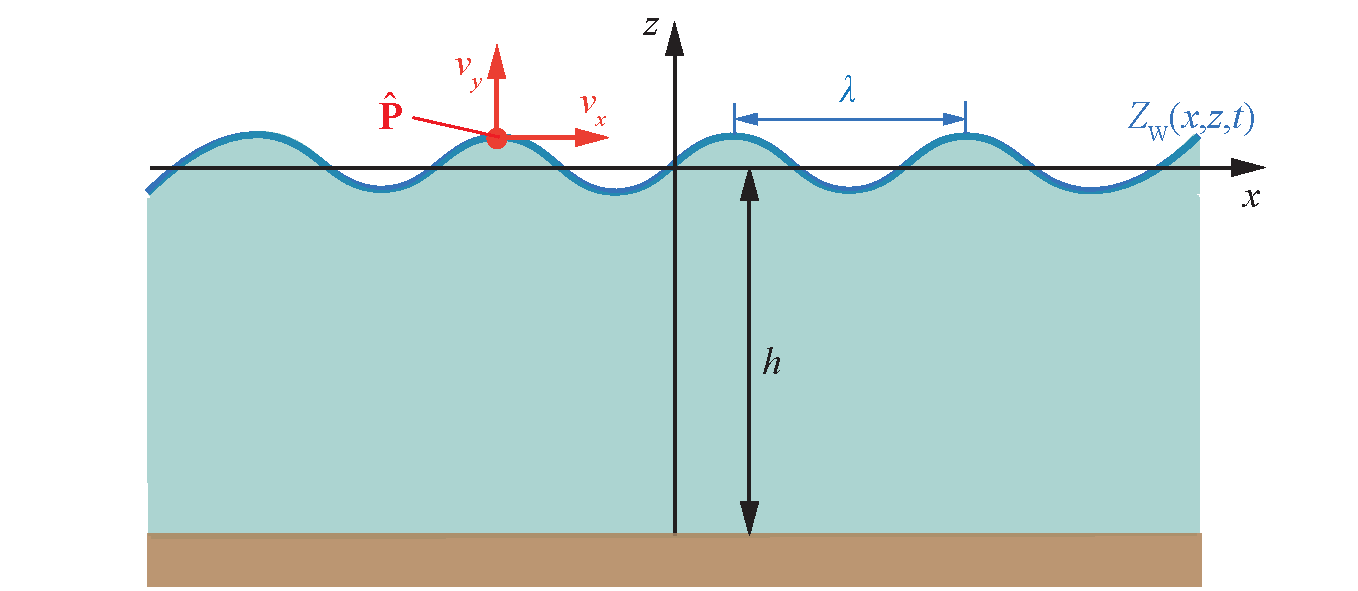
\includegraphics[width=\textwidth]{WasserwellenKoord.pdf}
  \captionof{figure}{Koordinatensystem f�r Wasserwellen.}%
  \label{abb:kontmech_Wasserwellen}
\end{center}

Zur L�sung des Problems m�ssen wir mehrere Gleichungen ber�cksichtigen. Als
erstes gehen wir von der Euler-Gleichung \eqref{eq:kontmech_EulerGleichung}
aus, in der wir entsprechend der Annahme �ber das Modell die
Geschwindigkeitskomponenten $v_x$ und $v_y$ ber�cksichtigen,
\begin{equation*}
  \vec{v} = \begin{pmatrix} v_x & 0 &v_z \end{pmatrix}^\text{T} \; .
\end{equation*}
Die Euler-Gleichung reduziert sich dann auf die Form
\begin{equation}
  \varrho \lk \lk v_x \frac{\partial}{\partial x} + v_z \frac{\partial}
  {\partial z} \rk \begin{pmatrix} v_x \\ 0 \\ v_z \end{pmatrix}
  + \frac{\partial}{\partial t} \begin{pmatrix} v_x \\ 0 \\ v_z \end{pmatrix}
  \rk =  - \begin{pmatrix} \partial p/\partial x \\ 0 \\
    \partial p/\partial z \end{pmatrix} + \varrho \begin{pmatrix} 0 \\ 0 \\ -g
  \end{pmatrix}\; .
  \label{eq:kontmech_WellenEulerGleichung}
\end{equation}

Da wir davon ausgehen, dass die Bewegung rotationsfrei zustande kommt
und eine reibungsfreie Fl�ssigkeit dann auch rotationsfrei bleibt (was in
\kap{kontmech_laminareStroemungenFluessigkeiten} genauer untersucht wird),
k�nnen wir das Geschwindigkeitsfeld auf eine skalare Funktion $\Psi(x,z,t)$
zur�ckf�hren,
\begin{equation}  \vec{v} = \nabla \Psi \; , \qquad v_x = \frac{\partial \Psi}
  {\partial x} \; , \quad v_z = \frac{\partial \Psi}{\partial z} \; .
  \label{eq:kontmech_WasserwellenPsi}
\end{equation}
Wir haben es also mit einer sogenannten \emph{Potentialstr�mung}\index{Str�mung!Potential-} zu tun. Ausgedr�ckt durch die skalare Funktion $\Psi(x,z,t)$ l�sst sich die vektorielle
Gleichung \eqref{eq:kontmech_WellenEulerGleichung} auf die skalare Darstellung
\begin{equation}
  \frac{\varrho}{2} \lk \frac{\partial \Psi}{\partial x} \rk^2
  + \frac{\varrho}{2} \lk \frac{\partial \Psi}{\partial z}  \rk^2
  + \varrho \frac{\partial \Psi}{\partial t} = - \varrho g z  - p + C
  \label{eq:kontmech_WellenEulerSkalar}
\end{equation}
mit einer beliebigen Konstanten $C$ zur�ckf�hren. Davon kann man sich leicht
�berzeugen, wenn man den Gradienten von Gleichung
\eqref{eq:kontmech_WellenEulerSkalar} bildet und dabei mit
\eqref{eq:kontmech_WasserwellenPsi} ber�cksichtigt, dass
$\Psi$ und $p$ nicht von der Koordinate $y$ abh�ngen.

Die Gleichung \eqref{eq:kontmech_WellenEulerSkalar} kann nun
herangezogen werden, den Druck im Wasser zu bestimmen. Eine wertvolle Information
f�r die Wellenausbreitung erhalten wir, indem wir ber�cksichtigen, dass
Gleichung \eqref{eq:kontmech_WellenEulerSkalar} insbesondere auch an der
Grenzschicht zwischen der Wasseroberfl�che und der Luft gelten muss. Hier
kennen wir den Druck und wissen, dass er (bis auf vernachl�ssigbar kleine
�nderungen mit $Z_W(x,t)$) konstant dem Atmosph�rendruck $p_\mathrm{atm}$
entsprechen muss. Da die Gleichung f�r jede beliebige Konstante $C$ gilt,
w�hlen wir zur Vereinfachung $C = -p_\mathrm{atm}$ und erhalten
\begin{equation}
  \frac{\varrho}{2} \lk \frac{\partial \Psi(x,z=0)}{\partial x} \rk^2
  + \frac{\varrho}{2} \lk \frac{\partial \Psi(x,z=0)}{\partial z}  \rk^2
  + \varrho \frac{\partial \Psi(x,z=0)}{\partial t} = - \varrho g Z_w(x,t)
  \; .
  \label{eq:kontmech_WellenEulerSkalarOberflaeche}
\end{equation}

Wasserwellen m�ssen dar�ber hinaus eine zweite Gleichung erf�llen. Da eine
kompressionsfreie Fl�ssigkeit vorliegt und wir in unserem Modell davon
ausgehen, dass es keinen Zu- oder Abfluss von Wasser, also keine Quellen und
keine Senken gibt, gilt die Form \eqref{eq:kontmech_KontinuitaetsglInkompr}
der Kontinuit�tsgleichung \eqref{eq:kontmech_KontinuitaetsglDiff}, die hier
 die Gestalt
\begin{equation}
  \frac{\partial v_x}{\partial x} + \frac{\partial v_z}{\partial z}
  = 0
  \label{eq:kontmech_WellenKontinuitaet}
\end{equation}
annimmt. Auch hier f�hren wir die skalare Funktion $\Psi(x,z)$ ein, was uns
auf 
\begin{equation}
  \frac{\partial^2 \Psi}{\partial x^2} + \frac{\partial^2 \Psi}{\partial z^2} = \Delta \, \Psi = 0
  \label{eq:kontmech_WellenKontPot}
\end{equation}
f�hrt. Eine Funktion $\Psi$, die die Wellen beschreibt, muss also zus�tzlich
zu \eqref{eq:kontmech_WellenEulerSkalarOberflaeche} die quellenfreie Laplace-Gleichung
\eqref{eq:kontmech_laplace_eq} erf�llen, was generell f�r Potentialstr�mungen gilt.

Die Eulergleichung und auch \eqref{eq:kontmech_WellenKontPot} sind partielle Differentialgleichungen \cite{Riley2006, Fischer2014}.
Deswegen m�ssen wir zus�tzlich noch die Randbedingungen ber�cksichtigten. Eine
davon haben wir oben schon durch Gleichung \eqref{eq:kontmech_WasserwellenRBLuft}
kennen gelernt, die sich durch Geschwindigkeiten ausdr�cken l�sst. Bildet man
auf beiden Seiten von \eqref{eq:kontmech_WasserwellenRBLuft} die Zeitableitung, erh�lt man
\begin{equation}
  v_z(z_0 = 0) = v_z(z = Z_W(x,t)) = \left . \frac{\partial \Psi}{\partial z}
  \right |_{z=Z_W(x,t)}
  = \frac{\partial Z_W(x,t)}{\partial x} v_x + \frac{\partial Z_W(x,t)}
  {\partial t} \; ,
  \label{eq:kontmech_WasserwellenRBvzLuft}
\end{equation}
was die ben�tigte Randbedingung an der Grenzschicht zur Luft darstellt. Sie
sagt aus, dass ein Materiepunkt an der Wasseroberfl�che genau die vertikale
Geschwindigkeit der Welle an der Oberfl�che haben muss. Das entspricht einem
Materiepunkt, der die Welle nicht verl�sst.

Die zweite Randbedingung ist am Boden bei $z=-h$ gegeben. Hier muss die
vertikale Geschwindigkeit der Welle verschwinden, denn die Materiepunkte
des Wassers k�nnen nicht in den Boden eindringen. Man erh�lt also die
Forderung
\begin{equation}
  v_z(z = -h) = \left . \frac{\partial \Psi}{\partial z} \right |_{z=-h}
  = 0 \; .
  \label{eq:kontmech_WasserwellenRBvzBoden}
\end{equation}

Insgesamt k�nnen wir festhalten, dass eine Wasserwelle, die durch den
Schweredruck dominiert wird, durch die skalare Form der Euler-Gleichung
an der Oberfl�che \eqref{eq:kontmech_WellenEulerSkalarOberflaeche}, durch
die Kontinuit�tsgleichung \eqref{eq:kontmech_WellenKontPot} sowie die
beiden Randbedingungen \eqref{eq:kontmech_WasserwellenRBvzLuft} und
\eqref{eq:kontmech_WasserwellenRBvzBoden} gegeben ist.

Analytische L�sungen lassen sich f�r Wellen mit Amplituden, die klein
im Vergleich zur Wellenl�nge $\lambda$ sind, finden. Tats�chlich ist das f�r Wasserwellen
oft erf�llt, sodass wir davon ausgehen und analytische L�sungen angeben
k�nnen. Dazu stellen wir erst fest, dass $\Psi$, $v_x$, $v_z$, $Z_W$ und
$\partial Z_W / \partial x$ alle von der Gr��enordnung der Amplitude sind
und auch in derselben Ordnung
\begin{equation}
  v_z(x,z=Z_W) = v_z(x,z=0)
\end{equation}
gilt. Wir beschr�nken uns auf Terme in der niedrigsten Ordnung, was dazu
f�hrt, dass alle quadratischen Terme in der skalaren Euler-Gleichung
\eqref{eq:kontmech_WellenEulerSkalarOberflaeche} und der Randbedingungn an
der Oberfl�che \eqref{eq:kontmech_WasserwellenRBvzBoden} vernachl�ssigt,
 \dh Null gesetzt werden k�nnen. Es verbleiben die Gleichungen
\begin{equation}
  \frac{\partial \Psi}{\partial t} = - g Z_W(x,t)
  \label{eq:kontmech_WellenEulerSkalarOberflaecheLin}
\end{equation}
und
\begin{equation}
    v_z(z = 0) = \left . \frac{\partial \Psi}{\partial z} \right |_{z=0}
  = \frac{\partial Z_W(x,t)}{\partial t} \; ,
  \label{eq:kontmech_WasserwellenRBvzLuftLin}
\end{equation}
die zusammen mit der unver�nderten (linearen) Kontinuit�tsgleichung
\eqref{eq:kontmech_WellenKontPot} und der ebenfalls schon linearen
Randbedingung am Boden \eqref{eq:kontmech_WasserwellenRBvzBoden} gel�st werden
m�ssen.

Als vern�nftigen Ansatz f�r diesen linearisierten Satz an
Differentialgleichungen k�nnen wir in $x$-Richtung eine sinusf�rmige Welle
annehmen. Die Kontinuit�tsgleichung \eqref{eq:kontmech_WellenKontPot} l�sst
sich nach Ableitungen in den Variablen $x$ und $z$ separieren. Das legt einen
Produktansatz (siehe dazu \ua \cite{Riley2006, Fischer2014}) mit einer
hyperbolischen Funktion nahe. Wir probieren es also mit
\begin{equation}
  \Psi(x,z,t) = \Psi_0 \cosh(k z + \varphi_1) \sin(\omega t - k x + \varphi_0)
  \; ,
  \label{eq:kontmech_WasswerwellenAnsatz1}
\end{equation}
worin wir $k = 2\pi/\lambda $ als sogenannte Wellenzahl\index{Wellenzahl} und $\omega = 2\pi/T$ als Kreisfrequenz der Wellenanregung mit der Periode $T$ eingef�hrt haben. Tats�chlich l�st dieser Ansatz die Kontinuit�tsgleichung. Die Konstante
$\varphi_1$ l�sst sich durch die Randbedingung
\eqref{eq:kontmech_WasserwellenRBvzBoden} einfach bestimmen, denn diese
fordert
\begin{equation*}
  \Psi_0 k \sinh(- k h + \varphi_1) \sin(\omega t - k x + \varphi_0)
  = 0
\end{equation*}
f�r jedes beliebige $x$ und $t$, was sich nur durch $\varphi_1 = kh$
erf�llen l�sst. Damit lautet unser Ansatz
\begin{equation}
  \Psi(x,z,t) = \Psi_0 \cosh \lk k (z + h) \rk
  \sin(\omega t - k x + \varphi_0) \; .
  \label{eq:kontmech_WasswerwellenAnsatz2}
\end{equation}

Nun m�ssen noch die Gleichungen
\eqref{eq:kontmech_WellenEulerSkalarOberflaecheLin} und
\eqref{eq:kontmech_WasserwellenRBvzLuftLin} erf�llt sein. Dazu leiten wir
\eqref{eq:kontmech_WellenEulerSkalarOberflaecheLin} nach der Zeit ab und
setzen sie in \eqref{eq:kontmech_WasserwellenRBvzLuftLin} ein. Zusammen mit
\eqref{eq:kontmech_WasserwellenPsi} erhalten wir
\begin{equation}
  \left . \frac{\partial \Psi}{\partial z} \right |_{z=0}
  = - \frac{1}{g} \left . \frac{\partial^2 \Psi}{\partial t^2} \right |_{z=0}
  \; .  \label{eq:kontmech_WasswerwellenAnsatz3}
\end{equation}
Setzt man in  \eqref{eq:kontmech_WasswerwellenAnsatz3} den Ansatz \eqref{eq:kontmech_WasswerwellenAnsatz2} ein,
erh�lt man nach geeignetem K�rzen
\begin{equation*}
  k \sinh(kh) = \frac{\omega^2}{g} \cosh(kh)\; ,
\end{equation*}
woraus man die \emph{Dispersionsrelation}\glslink{Dispersionsrelation} f�r Wasserwellen\index{Dispersionsrelation|textbf}
\begin{equation*}
  \omega^2 = g k \tanh(kh) 
  \label{eq:komtech_WasserwellenDispersion}
\end{equation*}
gewinnen kann, die die Wellenzahl $k$ (Inverse zur Wellenl�nge $\lambda$) in Beziehung zur Anregungsfrequenz $\omega$ setzt. Die Wasserh�he $h$ ist hierbei ein Parameter. Daraus ergibt sich die \gls{Phasengeschwindigkeit} der Welle\index{Phasengeschwindigkeit|textbf}
\begin{equation}
  v_\mathrm{ph} = \frac{\omega}{k} = \sqrt{\frac{g}{k} \tanh(kh)} \; .
\end{equation}

Zum Schluss wollen wir uns noch zwei wichtige Grenzf�lle dieser
Dispersionsrelation anschauen.
\begin{itemize}
\item Im relativ flachen Wasser sei $h\ll \lambda = 2\pi/k$ und man kann $\tanh(kh) \approx kh$
  n�hern, sodass gilt
  \begin{equation}
    %\omega^2 \approx g k^2 h = 4\pi^2\,g\,h/\lambda^2; \qquad \text{bzw.} \qquad
    %v_\mathrm{ph} \approx \sqrt{gh} \; .
    \omega^2 \approx g k^2 h = \frac{4\pi^2\,g\,h}{\lambda^2} \qquad \text{\bzw} \qquad
    v_\mathrm{ph} \approx \sqrt{gh} \; .
  \end{equation}
\item Im tiefen Wasser (\zb im Ozean) gilt dagegen $h\gg \lambda = 2\pi/k$ und $\tanh(kh) \approx 1$, was
  auf
  \begin{equation}
    %\omega^2 \approx g k = 2\pi\,g/\lambda\; \qquad \text{bzw.} \qquad
    %v_\mathrm{ph} \approx \sqrt{1/(2\pi)}\sqrt{g\,\lambda}
    \omega^2 \approx g k = \frac{2\pi\,g}{\lambda}\; \qquad \text{bzw.} \qquad
    v_\mathrm{ph} \approx \sqrt{\frac{1}{2\pi}}\sqrt{g\,\lambda}
  \end{equation}
  f�hrt. Wie zu erwarten ist, hat der Boden hier keinen Einfluss, die
  Dispersionsrelation und die Phasengeschwindigkeit h�ngen nicht von der H�he
  $h$ ab.

  Wir werden die Ergebnisse bei der Berechnung von Gezeitenwellen in der
  Himmelsmechanik im Band II verwenden. Eine sehr sch�ne Simulation der
  Wasserwellen auf Basis der vorgestellten Theorie findet man in
  \cite{Girwidz2023}.
\end{itemize}

\end{example}
%BEISPIEL %%%%%%%%%%%%%%%%%%%%%%%%%%%%%%%%%%%%%%%%%%%%%%%%%%%%%%%%%%%%%%%%%%%%%%%%%%%%%%%%%%


\subsubsection{Bernoulli-Gleichung}
\label{kap:kontmech_BernoulliGl}\index{Bernoulli-Gleichung}

Mit dem Wissen �ber die Euler-Gleichung
\eqref{eq:kontmech_EulerGleichung} kann man weitere Schlussfolgerungen
f�r die Bewegung von Fluiden erhalten, die f�r viele Anwendungen
interessant sind. Dazu halten wir nochmals fest, dass Kr�fte Arbeit verrichten
k�nnen, wie wir es bereits aus der Mechanik von Massepunkten �ber Gleichung
\eqref{eq:bew_Arbeit_infinitesimal} kennen. Wir betrachten im Folgenden das
Beispiel eines idealisierten Fluids ohne Reibungseffekte.

In einer station�ren Fluid-Str�mung ($\d \vec{v} /\d t = 0$) durch ein Rohr mit einem ver�nderlichen Querschnitt,
wie \zb in \figref{kontmech_StroemungBernoulli} dargestellt,
muss die Geschwindigkeit des Mediums an den verschiedenen Querschnitten
(\zb $A_1$ und $A_2$) in der Abbildung unterschiedlich sein, denn andernfalls
m�sste sich an manchen Stellen Masse ansammeln oder verringern, was einer
station�ren Str�mung widerspr�che.

\begin{figure}
  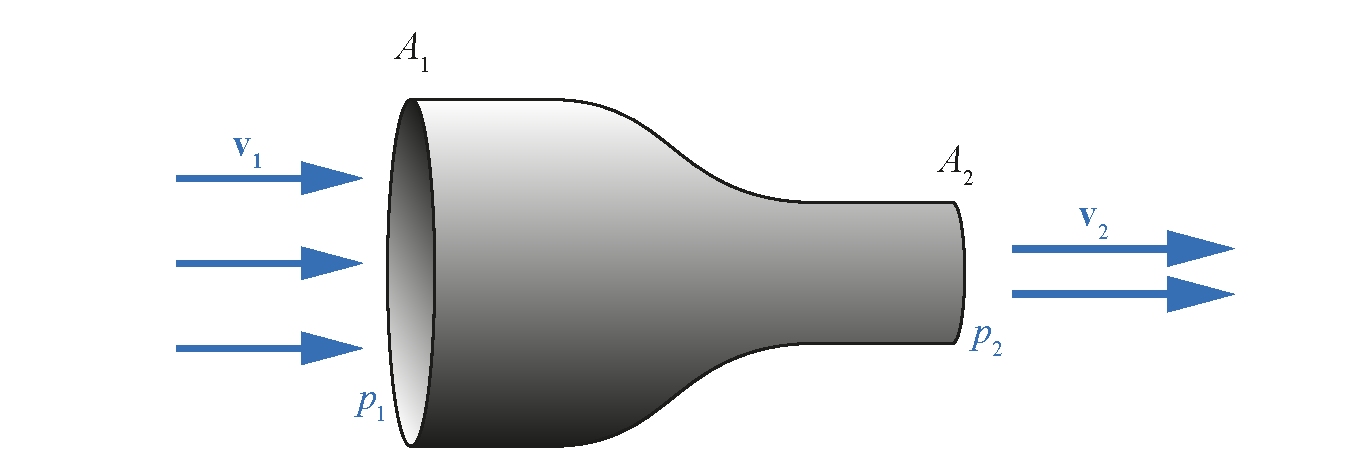
\includegraphics[width=\textwidth]{StroemungBernoulli.pdf}
  \caption[Zur Bernoulli-Gleichung]{Zur Bernoulli-Gleichung: Str�mung durch
    ein Rohr mit unterschiedlichen Querschnitten entlang der Koordinate $x$. Die Geschwindigkeit muss an
    den Querschnitten $A_1$ und $A_2$ in einer station�ren Str�mung einer
    inkompressiblen Fl�ssigkeit verschieden sein. Das hat Auswirkungen
    auf den Druck in den beiden Rohrbereichen.}
  \label{abb:kontmech_StroemungBernoulli}
\end{figure}

Damit die Geschwindigkeit unterschiedlich sein kann, muss das Gas jedoch entlang der Koordinate $x$
beschleunigt werden. Nach der Euler-Gleichung \eqref{eq:kontmech_EulerGleichung}
kann die Beschleunigung in Abwesenheit von �u�eren Kr�ften und Reibung
allein durch den Druck aufgebracht werden. Tats�chlich transportiert der
Druck $p$ die Fl�ssigkeit oder das Gas entlang des Weges $\D x$ durch das Rohr mit Querschnitt $A$ und
verrichtet dabei die Arbeit
\begin{equation}
  \Delta W = \Delta p \,A \,\D x = \Delta p \,\D V \; .
  \label{eq:kontmech_ArbeitBernoulli}
\end{equation}
Diese Arbeit f�hrt zur Beschleunigung und damit zur �nderung der kinetische
Energie.

Die Str�mung kommt mit dieser Erkl�rung dadurch zustande, dass ein
Massenelement von seinem nachfolgenden eine Kraft erf�hrt und diese an das
Massenelement vor ihm weitergibt. Ist der Rohrquerschnitt konstant, gleichen
sich diese Kr�fte gerade aus und die Geschwindigkeit bleibt konstant. Ein
Massenelement
\begin{equation}
  \D m = \varrho\,\D V \; ,
  \label{eq:kontmech_Massenelement}
\end{equation}
das gerade am �bergang zwischen den beiden Rohrabschnitten ist, wird im
Rohrabschnitt mit dem Querschnitt $A_1$ beschleunigt und beschleunigt selbst
ein weiteres Massenelement im Rohrabschnitt mit dem Querschnitt $A_2$. Diese
Arbeitsleistungen m�ssen unterschiedlich sein, damit eine �nderung der
kinetischen Energie auftreten kann. F�r eine inkompressible Fl�ssigkeit ist
$\varrho$ konstant und nach den Gleichungen \eqref{eq:kontmech_ArbeitBernoulli}
und \eqref{eq:kontmech_Massenelement} ist das nur m�glich, wenn der
Druck in beiden Rohrabschnitten unterschiedlich ist. Dieser l�sst sich sogar
aus der Energieerhaltung berechnen. Dazu stellen wir zun�chst fest, dass
die Differenz der kinetischen Energie des Gases im Rohrabschnitt mit dem Querschnitt $A_2$
und der im Abschnitt mit $A_1$ aus der Differenz der Arbeitsleitungen ergeben muss:
\begin{equation*}
  \Delta T = \frac{1}{2} \varrho \, \D V \, u_2^2 - \frac{1}{2} \varrho \, \D V \, u_1^2
  =  \Delta W = p_1 \,\D V - p_2 \,\D V = \Delta p \D V \,.
\end{equation*}
Dies l�sst sich zur \emph{Bernoulli-Gleichung}\index{Bernoulli-Gleichung}
\begin{equation}
  \frac{1}{2} \varrho \, u_1^2 + p_1 = \frac{1}{2} \varrho \, u_2^2 +  p_2
  \label{eq:kontmech_BernoulliGl}
\end{equation}
umformen. Die Konstante
\begin{equation}
  p_0 = \frac{1}{2} \varrho \, u^2 + p 
  \label{eq:kontmech_Staudruck}
\end{equation}
l�sst sich als der Druck interpretieren, den die Fl�ssigkeit ruhend (also
im Grenzfall eines unendlich breiten Rohres) annehmen w�rde. Der Druck $p$
ist der \emph{statische Druck der str�menden Fl�ssigkeit}\index{Druck!statischer}.
Die Bernoulli-Gleichung ist eine der Grundgleichungen f�r die Behandlung von Str�mungen in Fluiden und ist Grundlage vieler aero- und hydrodynamischer Berechnungen in der Technik. Sie wurde vom Sohn Daniel\indexp{Bernoulli, Daniel}\footnote{Daniel Bernoulli (1700 -- 1782) war ein Schweizer Mathematiker und Physiker, der eng mit Leonhard Euler zusammen arbeitete.} und Vater Johann Bernoulli\indexp{Bernoulli, Johann}\footnote{Johann Bernoulli (1667 -- 1748) war Schweizer Mathematiker und Arzt.
  Er arbeitete unter anderem auf dem Gebiet der Reihen und Differentialgleichungen.} aufgestellt.\\
Wir haben hier die Bernoulli-Gleichung aus energetischen �berlegungen (Energieerhaltung, da keine Reibung) hergeleitet. Man kann sie auch direkt aus der Euler-Gleichung \eqref{eq:kontmech_EulerGleichung} herleiten (\probref{kontmech_bernoulli}).

% BEISPIEL %%%%%%%%%%%%%%%%%%%%%%%%%%%%%%%%%%%%%%%%%%%%%%%%%%%%%%%%%%%%%%%%%%%%%%%%%%%%%%%%%%
\begin{example}{Schiff in einem Kanal}
\label{bsp:kontmech_SchiffKanal}
\smallskip

Der unterschiedliche statische Druck bei unterschiedlichen
Flie�geschwindigkeiten macht sich auch in der Schifffahrt bemerkbar. Im M�rz
2021 legte sich das Containerschiff "`Ever Given"' im Suezkanal quer und
blockierte diesen f�r mehrere Tage. Daf�r kann unter anderem der
Druckunterschied in str�menden Fl�ssigkeiten verantwortlich gemacht werden
\cite{Woehrbach2021}. Um dies darzustellen, soll
\figref{kontmech_SchiffKanalStroem} als Skizze dienen.

\begin{center}
  
\includegraphics[width=\textwidth]{SchiffKanalStroem.pdf}
  \captionof{figure}{Str�mungen um ein Schiff in einem Kanal.}%
  \label{abb:kontmech_SchiffKanalStroem}
\end{center}

F�hrt das Schiff nicht in der Mitte des Kanals, muss das ausweichende Wasser an
beiden Seiten des Schiffes mit unterschiedlichen Geschwindigkeiten flie�en.
Dies bewirkt eine seitliche Kraft auf das Schiff. Durch die Form des Schiffes
gibt es aber auch einen Unterschied in den seitlichen Kr�ften zwischen Bug und
Heck des Schiffes, was in einem Drehmoment resultiert.
Im eingezeichneten Beispiel ist die Str�mungsgeschwindigkeit links vom Schiff
kleiner als rechts. Damit ist aber der statische Druck auf der linken Seite
gr��er als auf der rechten. Es resultiert eine Kraft nach rechts. Am Bug
sind die Str�mungsunterschiede geringer als am Heck. Das hei�t, die
resultierende Kraft ist am Heck gr��er als am Bug. Folglich wird sich das
Schiff mit dem Heck nach rechts drehen.
\probref{kontmech_SchiffKanal} besch�ftigt sich ausf�hrlicher mit einem
solchen Beispiel.
\end{example}
%BEISPIEL %%%%%%%%%%%%%%%%%%%%%%%%%%%%%%%%%%%%%%%%%%%%%%%%%%%%%%%%%%%%%%%%%%%%%%%%%%%%%%%%%%



\subsubsection{Innere Reibung}
\label{kap:kontmech_InnereReibung}\index{Reibung!innere}\index{Viskosit�t|textbf}

Wenn sich Fl�ssigkeiten und Gase bewegen, sto�en die einzelnen Atome
oder Molek�le aneinander und �bertragen dabei einen Impuls. Dies entspricht
einer inneren Kraftwirkung oder einer inneren Reibung. Um diese quantifizieren
zu k�nnen, betrachten wir die Situation aus \figref{kontmech_InnereReibung1}a.
Eine Fl�ssigkeit ist zwischen zwei Platten eingesperrt. Die rechte Platte
wird mit einer konstanten Geschwindigkeit $\vec{v}_0 = v_0\,\veceZ$ gegen die
linke verschoben. Dabei sp�rt man den Widerstand durch die innere Reibung.

\begin{figure}
  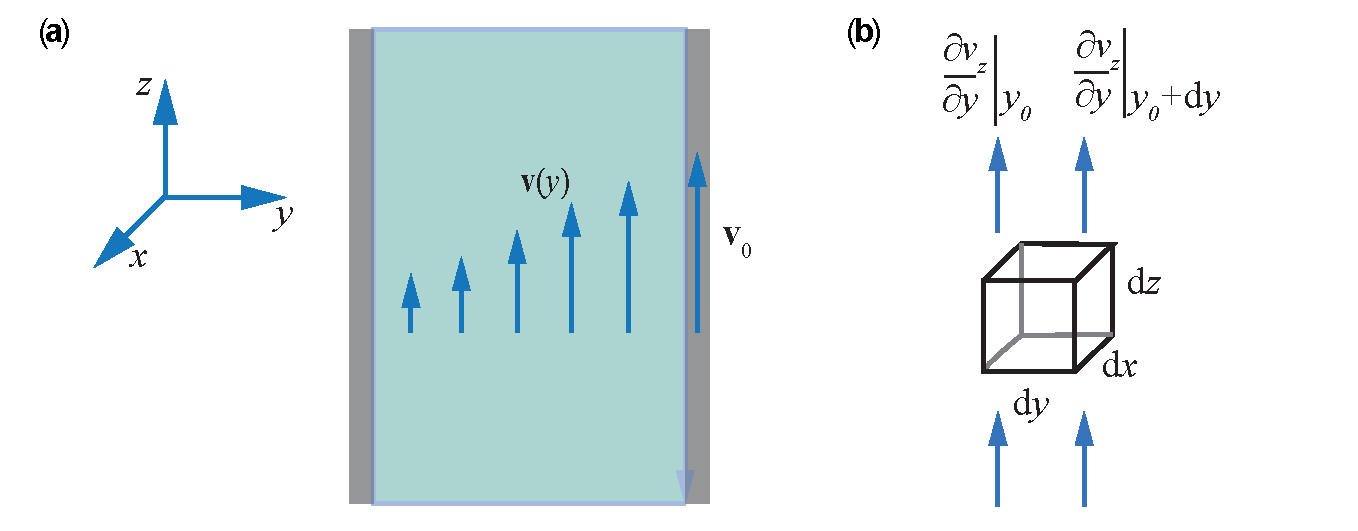
\includegraphics[width=\textwidth]{InnereReibung.pdf}
  \caption[Innere Reibung in einer Fl�ssigkeit]{\fa Eine Fl�ssigkeit ist
    zwischen zwei Platten eingespannt. Die rechte Platte wird mit $\vec{v}_0
    = v_0 \, \veceZ$ gegen die linke bewegt. In der Fl�ssigkeit bildet sich ein
    Geschwindigkeitsgradient aus. \fb F�r die Kraft auf ein Volumenelement
    $\D V = \D x\, \D y\, \D z$ m�ssen die Reibungen an allen Fl�chen beachtet
    werden. Hier werden sie bei $y_0$ und $y_0 + \D y$ unterschiedlich
    angenommen.}
  \label{abb:kontmech_InnereReibung1}
\end{figure}

Die Fl�ssigkeitsmolek�le sind an den R�ndern mit beiden
Platten in Kontakt und haben daher mit diesen die gleiche Geschwindigkeit. Innerhalb
der Fl�ssigkeit herrscht also ein Geschwindigkeitsgradient in $y$-Richtung.
Da die Kraftwirkung nur durch die Impuls�bertragung zwischen den
Fl�ssigkeitsmolek�len zustande kommen kann, k�nnen wir folgende Abh�ngigkeiten
voraussetzen:
\begin{itemize}
\item Die Kraft zwischen zwei Schichten der Fl�ssigkeit ist nach den
  Newtonschen Bewegungsgleichungen \eqref{eq:bew_NewtonBGL} proportional zur
  Impuls�nderung und damit zum Geschwindigkeitsgradienten.
\item Die Kraft muss proportional zur Zahl der sto�enden Molek�le sein. Diese
  ist jedoch, da sie (in einer Fl�ssigkeit immer, in einem Gas zumindest im
  Mittel) einen festen Raum einnehmen, proportional zur Fl�che $A$ der Grenze
  zwischen zwei Fl�ssigkeitsschichten. 
\end{itemize}
Wir erhalten f�r die Kraft
\begin{equation}
  \vec{F}_\text{R} = \eta \, A \, \frac{\partial v_z}{\partial y}
  \veceZ \; ,
  \label{eq:kontmech_ReibungskraftInnere}
\end{equation}
wobei wir den Proportionalit�tsfaktor $\eta$ als \emph{Viskosit�t}\glslink{viskositaet} bezeichnen\index{Viskosit�t}. Die Viskosit�t hat die Einheit
$\SI{}{\newton \second \per \metre^2}$ und beschreibt die
Eigenschaft der Fl�ssigkeit oder des Gases, Widerstand gegen eine
Bewegungs�nderung zu leisten.

Diese Kraft beschreibt bisher aber nur, welche Reibung an der Grenze zwischen
zwei Schichten der Fl�ssigkeit oder des Gases entsteht. Wollen wir die Kraft
wissen, die auf ein Volumen $\D V$ der Fl�ssigkeit wirkt, m�ssen wir uns
ein solches Fl�ssigkeitsvolumen herausschneiden, wie es in
\figref{kontmech_InnereReibung1}b eingezeichnet ist. Auf der rechten Seite
wird das Volumen von der angrenzenden Schicht beschleunigt, $\D V$ erf�hrt
also eine Kraft in positive $z$-Richtung. Auf der linken Seite ist es
das Volumenelement $\D V$ selbst, das die angrenzende Schicht beschleunigt und
dabei selbst eine Kraft in negative $z$-Richtung erf�hrt. Insgesamt ergibt
sich damit nach \eqref{eq:kontmech_ReibungskraftInnere} die Kraft
\begin{equation}
  \vec{F}_{\text{R},y} = \eta \lk {\frac{\partial v_z}
    {\partial x}}\big|_{y_0 + \D y} - {\frac{\partial v_z}{\partial y}}\big|_{y_0}
  \rk \,\veceZ \, \D x \, \D z\; .
\end{equation}
Liegen am linken und am rechten Rand identische Geschwindigkeitsgradienten vor,
sieht man sofort, dass das Volumenelement $\D V$ keine resultierende Kraft
erf�hrt. Im Allgemeinen ist das aber nicht der Fall. Sehr sicher k�nnen wir
 davon ausgehen, dass wir f�r den differentiellen Abstand $\D y$ eine
Linearisierung des Gradienten durchf�hren k�nnen. Wir setzen also an:
\begin{equation}
  \frac{\partial v_z}{\partial y}\big|_{y_0 + \D y} =
  \frac{\partial v_z}{\partial y}\big|_{y_0} + \frac{\partial^2 v_z}
  {\partial y^2}\big|_{y_0}  \D y \; . 
\end{equation}
F�r die Kraft auf das Volumenelement ergibt sich somit
\begin{subequations}
  \begin{align}
    \vec{F}_{\text{R},y} &= \eta \lk \killA{\frac{\partial v_z}
      {\partial y}\big|_{y_0}} +  \frac{\partial^2 v_z}{\partial y^2}\big|_{y_0} \D y
      - \killA{\frac{\partial v_z}{\partial y}\big|_{y_0}} \rk \, \veceZ\, \D x \, \D z 
    = \eta \, \frac{\partial^2 v_z}{\partial y^2}\big|_{y_0}\, \veceZ\, \D V \; .
    %&= \eta \, \frac{\partial^2 v_z}{\partial y^2}\big|_{y_0 }\, \veceZ\,\D x \, \D y \, \D z
  \end{align}
  Vollkommen analog �berlegt man sich, dass bei einem vorhandenen
  Geschwindigkeitsgradienten in $x$-Richtung gilt, dass
  \begin{equation}
    \vec{F}_{\text{R},x} = \eta \, \frac{\partial^2 v_z}
    {\partial x^2}\big|_{y_0}\,\veceZ\, \D V \; .
  \end{equation}
\end{subequations}
Ist die Bewegung einer inkompressiblen Fl�ssigkeit nicht entlang der
$z$-Richtung ausgerichtet, sondern besitzt sie auch zumindest eine Komponente
in $x$- oder $y$-Richtung, so ist dieselbe �berlegung f�r einen Gradienten
(bzw. einen sich �ndernden Gradienten) in $z$-Richtung m�glich.\footnote{Ein
Geschwindigkeitsgradient in $z$-Richtung tritt nat�rlich auch bei Str�mungen
mit sich �ndernden Querschnitten (siehe \kap{kontmech_BernoulliGl})
oder bei kompressiblen Fl�ssigkeiten auf, wenn die Bewegung allein in
$y$- \bzw $z$-Richtung erfolgt.} Im allgemeinen Fall erh�lt man mit dem
Laplace-Operator \eqref{eq:kontmech_laplace_eq}
\begin{equation*}
  \Delta = \frac{\d^2}{\d x^2} + \frac{\d^2}{\d y^2} + \frac{\d^2}{\d z^2} 
\end{equation*}
f�r die gesamten Kr�fte, die sich durch die Reibung der Schichten aneinander
auf das Volumenelement $\D V$ ergeben
\begin{align}
  \vec{F}_{\text{R}} &= \eta \, \Delta \vec{v}\big|_{(x_0, y_0, z_0)} \, \D V
  = \eta \, \Delta \vec{v}\big|_{\vec{r}_0} \, \D V ~~~\text{\bzw}~~~ \vec{f}_{\text{R}} = \eta \, \Delta \vec{v}\big|_{\vec{r}_0} \; .
\label{eq:kontmech_InnereReibung}
\end{align}

\subsection{Navier-Stokes-Gleichung}
\label{kap:kontmech_NavierStokes}\index{Navier-Stokes-Gleichung|textbf}

Nachdem wir nun einzelnen Kraftterme auf Basis der Euler-Gleichung untersucht und insbesondere die innere
Reibung eines Fluids gekl�rt haben, k�nnen wir die erhaltenen Beziehungen
in die Euler-Gleichung \eqref{eq:kontmech_EulerGleichung} \bzw \eqref{eq:kontmech_WellenEulerGleichung} einsetzen. Mit
der Druckkraft \eqref{eq:kontmech_Druckkraft} und der inneren Reibungskraft
\eqref{eq:kontmech_InnereReibung} erh�lt man dann die \emph{Navier-Stokes-Gleichung}
\begin{equation}
  \varrho \lk \lk \vec{v} \cdot \nablav \rk \vec{v} + \frac{\partial}{\partial t}
  \vec{v} \rk = \vec{f}_\text{V}  + \eta \, \Delta \vec{v} - \nablav p \; ,
  \label{eq:kontmech_NavierStokes}
\end{equation}
in der nur noch die Kraftdichte $\vec{f}_\text{V}$ der von au�en wirkenden
Volumenkr�fte nicht explizit gegeben sind. Sie ist eine partielle Differentialgleichung in $\vec{v}(\vec{r},t)$ bei gegebenen externen Kr�ften $ \vec{f}_\text{V}$ und statischen Druck $p$. 
%Letztere h�ngen nat�rlich von der Wechselwirkung mit der Umgebung ab. 
Wir m�chten darauf hinweisen, dass die \NVS \eqref{eq:kontmech_NavierStokes} in der Form \eqref{eq:kontmech_NavierStokes}
nur f�r inkompressible Fluide gilt. Es gibt auch eine \NVS f�r kompressible Fluide, die noch etwas komplizierter ist. Wir verweisen dazu auf \cite{Garvin2023}.
Wie bei jeder PDGL m�ssen die Randbedingungen f�r das betrachtete Volumen ber�cksichtigt werden. Die Navier\footnote{Claude Louis Marie Henri Navier (1785 -- 1836) war ein franz�sischer Mathematiker, Bauingenieur und Physiker. Er brachte die Elastizit�tstheorie in eine mathematisch handhabbare Form und gilt auch als Begr�nder der Baustatik. 1822 gab er die Navier-Stokes-Gleichungen f�r die Bewegung einer viskosen Fl�ssigkeit an.}\indexp{Navier, Claude Louis Marie Henri}-Stokes
%\footnote{Sir George Gabriel Stokes\indexp{Stokes, Sir George Gabriel} (1819--1903) war ein irischer Mathematiker und Physiker. Er arbeitete auf dem Gebiet der mathematischen und experimentellen Physik und besch�ftigte sich haupts�chlich mit der Hydrodynamik, der Elektrodynamik und der Akustik.}
-Gleichung\indexp{Stokes, Sir George Gabriel} ist damit eine Spezifizierung der Euler-Gleichung der Kontinuumsmechanik bez�glich der inneren Reibung und insbesondere der Einf�hrung der Viskosit�t.
Die partielle Differentialgleichung stellt eine gro�e mathematische Herausforderung dar, es ist nicht bekannt, ob es f�r den allgemeinen dreidimensionalen Fall eine �berall definierte (eindeutige) L�sung gibt. Die Frage nach der L�sung dieser Gleichung in ihrer allgemeiner Form  geh�rt daher zu den gro�en ungel�sten mathematischen Problemen und stellt eines der sogenannten sieben Millennium-Probleme\footnote{Als Millennium-Probleme wurden im Jahr 2000 durch das \textit{Clay Mathematics Institute (CMI)} in Cambridge (Massachusetts, USA) sieben ungel�ste mathematische Problem in einer Liste zusammen gefasst. F�r die L�sung eines der sieben Probleme wurde jeweils ein Preisgeld von einer Million US-Dollar ausgelobt.} dar.\\
Drei generelle Bemerkungen seien zur \NVS noch gemacht.
\begin{itemize}
	\item Die dominante, \dh gesuchte Variable in der \NVS ist der Geschwindigkeitsvektor $\vec{v}$. Der Druck ist \ia ebenfalls unbekannt, w�hrend wie erw�hnt die Dichte (f�r die inkompressible Fl�ssigkeit) und die externen Kr�fte als bekannt angenommen werden k�nnen. Die \NVS ist eigentlich in Komponenten geschrieben ein Set von drei Gleichungen. Wir haben aber vier Unbekannte, die 3 Komponenten der Geschwindigkeit (als Funktion von Ort und Zeit) und den Druck. Die dazu notwendige vierte Gleichung ist die Kontinuit�tsgleichung \eqref{eq:kontmech_KontinuitaetsglDiff}, die f�r die inkompressible Fl�ssigkeit durch $\nablav \vec{v} = 0$ gegeben ist.  
	\item Der Druck taucht in der Gleichung nur in Form $\nablav p$ auf. Das bedeutet, dass die Dynamik von inkompressiblen Fluiden immer nur von Druckdifferenzen abh�ngt und nicht von den Absolutwerten des Drucks, was relativ einsichtig ist.
	\item Wegen des Terms $\lk \vec{v} \cdot \nablav \rk \vec{v}$ ist die Differentialgleichung nichtlinear, dieser Term stellt die eigentliche Schwierigkeit in der L�sung der DGL dar.
\end{itemize}
Zwei wichtige l�sbare Spezialf�lle der Navier-Stokes-Gleichung sollen aber explizit genannt werden, zum einen der Fall, in dem jegliche von au�en angreifende Volumenkr�fte fehlen,
\begin{subequations}
  \begin{align}
    \varrho \lk \lk \vec{v} \cdot \nablav \rk \vec{v} + \frac{\partial}
    {\partial t} \vec{v}  \rk &= \eta \, \Delta \vec{v} - \nablav p \; ,
              \label{eq:kontmech_NavierStokesFrei} \\
    \intertext{und zum anderen der Fall, in dem eine Fl�ssigkeit oder ein Gas sich im homogenen Gravitationsfeld befindet, welches eine Kraftdichte $\varrho\,\vec{g}$ hat} 
    \varrho \lk \lk \vec{v} \cdot \nablav \rk \vec{v} + \frac{\partial}
    {\partial t} \vec{v} \rk &= \varrho\,\vec{g} + \eta \, \Delta \vec{v}
                               - \nablav p \; .
              \label{eq:kontmech_NavierStokesSchwerefeld}
  \end{align}
\end{subequations}



% BEISPIEL %%%%%%%%%%%%%%%%%%%%%%%%%%%%%%%%%%%%%%%%%%%%%%%%%%%%%%%%%%%%%%%%%%%%%%%%%%%%%%%%%%
\begin{example}{�berlegungen zu Str�mungen anhand des Stra�enverkehrs}
  \label{bsp:VerkehrKreuzung}
  \smallskip
  Wie bereits erw�hnt werden Methoden der Kontinuumsmechanik in vielen anderen Gebieten zur Problembeschreibung und -l�sung verwendet.
	Angeregt von einer Aufgabe in \cite{Meschede2010} m�chten wir uns zum
  Abschluss des Abschnitts ein Beispiel zur Kinematik und Dynamik des
  Stra�enverkehrs geben und zeigen wie auch in diesem Gebiet Begriffe aus der Kontinuumsmechanik, wie Str�mungen \usw verwendet werden k�nnen und damit auch veranschaulicht werden.
	Selbstverst�ndlich
  lassen sich viele weitere analoge Bilder finden. Wir m�chten insbesondere folgende
  heranziehen:

\begin{itemize}
\item \textbf{Beispiele f�r Strom- und Bahnlinien.}\\
  Stromlinien lassen sich aus den momentanen Geschwindigkeiten der Autos
  im Stra�enverkehr bilden. Wir m�ssen diese ermitteln und Linien einzeichnen,
  die tangential an diesem Feld liegen. Bahnlinien sind die tats�chlich
  gefahrenen Wege der einzelnen Autos. In einem station�r flie�enden Verkehr sind Strom-
  und Bahnlinien identisch, auf einspurigen Stra�en ohne Abzweigungen sind sie
  das sogar immer. Sie unterscheiden sich, wenn ein Auto spontan beschleunigt. Das
  kann \zb bei einem Spurwechsel ober beim Abbiegen an einer Kreuzung der Fall
  sein.
  
\item \textbf{Messen des Flusses.}\\
  Den Fluss bestimmt man, indem man die Autos z�hlt, die einen Querschnitt der
  Stra�e in einem festen Zeitintervall durchqueren.

\item \textbf{Kompressibilit�t und Inkompressibilit�t der Fahrzeugstr�mung.}\\
  In einem station�r flie�enden Verkehr ist die Fahrzeugstr�mung immer
  inkompressibel. Am Stauende einer Autobahn oder vor einer roten Ampel an
  einer Kreuzung hingegen verdichten sich die Autos. Hinter einer Verengung (z.B. auf
  einer Autobahn hinter einer Baustelle) beschleunigen sie wieder. Im
  Allgemeinen ist der Stra�enverkehr (Autodichte) also kompressibel.
  
\item \textbf{Divergenz- und Rotationsfreiheit. Beispiele f�r Quellen und
    Senken.}\\
  Divergenzfrei w�rde bedeuten, es k�nnen nie mehr oder weniger Autos im
  Verkehr werden. Global betrachtet stimmt das, aber definitiv nicht f�r
  eine einzelne Stra�e. Eine Autobahnausfahrt ist eine Senke, eine Auffahrt
  eine Quelle f�r Autos auf der Autobahn. Entsprechend k�nnen im Stadtverkehr
  an einer Kreuzung Autos von der Hauptstra�e abfahren (Senke f�r den Verkehr
  auf der Hauptstra�e) oder auf sie auffahren (Quelle).

  Rotationsfrei ist der Verkehr \iA ebenfalls nicht. Neben dem
  Kreisverkehr gibt es aber auch weitere Beispiele. Eine Rotation liegt
  bereits dann vor, wenn auf einer mehrspurigen Stra�e nicht auf allen
  Spuren gleich schnell gefahren wird. Auf einer Autobahn ist das, bis auf
  Ausnahmen wie \zb dichter Verkehr, immer der Fall.
  
\item \textbf{Beispiele f�r beide Terme der materiellen Beschleunigung.}\\
  Die Geschwindigkeit eines Autos h�ngt nat�rlich vom Geschwindigkeitsfeld
  des Verkehrs ab. Stellen wir uns eine Stra�e vor, auf der in verschiedenen
  Abschnitten unterschiedliche Geschwindigkeiten gelten, \zb $\SI{30}{\kilo
    \metre \per \hour}$ vor einer Schule, sonst $\SI{50}{\kilo
    \metre \per \hour}$. Vor der Schule bremsen alle Autos, dahinter
  beschleunigen sie. Das entspricht dem ersten Term der materiellen
  Beschleunigung in \eqref{eq:kontmech_Beschleunigung}, der beschreibt, dass ein Auto in ein anderes
  Geschwindigkeitsfeld ger�t. Ein einzelnes Auto, dessen Fahrer es eventuell
  eilig hat, kann ein anderes vor der Schule �berholen. Es weicht von der
  Geschwindigkeit aller Autos ab und wird einzeln beschleunigt. Das entspricht
  dem zweiten Term in Gleichung \eqref{eq:kontmech_Beschleunigung}.
  
\item \textbf{Analoga zu den Termen der Navier-Stokes-Gleichung.}\\
  In der Navier-Stokes-Gleichung tritt die materielle Beschleunigung auf
  (siehe oben). Diese wird von innerer Reibung beeinflusst. In der
  Annahme, dass wir keine Unf�lle haben, sich die Autos also nicht ber�hren,
  wird die innere Reibung dadurch gegeben, dass ein Auto nicht mit anderen
  zusammensto�en m�chte und \zb hinter einem langsamer werdenden Auto
  abbremsen muss, um nicht auf dies aufzufahren. Dies entspricht dem
  Viskosit�tsterm. Der Druckgradient entspricht z.B. einer roten Ampel (h�herer
  Druck vor dem Auto) oder einer gr�nen Ampel (niedrigerer Druck vor dem Auto).
	�u�ere Kr�fte k�nnen z.B. Hangabtriebskr�fte auf einer Strecke mit
  Steigung oder Gef�lle sein.   
  \end{itemize}

\end{example}
%BEISPIEL %%%%%%%%%%%%%%%%%%%%%%%%%%%%%%%%%%%%%%%%%%%%%%%%%%%%%%%%%%%%%%%%%%%%%%%%%%%%%%%%%%

Wir verweisen am Ende dieses Kapitels noch einmal auf Tabelle \ref{tab:kontmech_stroemung_overview}, in der wir die verschiedenen Str�mungsarten zusammengefasst haben. Wir wollen uns daran anschlie�end etwas n�her mit dem Spezialfall der laminaren Str�mungen besch�ftigen.
\begin{table}
\caption[�bersicht der verschiedenen Str�mungsarten.]{�bersicht der verschiedenen Str�mungsarten.}
\begin{tabular}{L{3cm}L{4.5cm}L{4.5cm}}
  \hline\noalign{\smallskip}
  Charakterisierung &  &    \\
  \noalign{\smallskip}\svhline\noalign{\smallskip}
	nach innerer Reibung&ideal Fluide\index{Fluid!ideales}, ohne innerer Reibung \linebreak $\eta =0$ &reale Fluide\index{Fluid!reales}, mit innerer Reibung \linebreak $\eta \neq 0$\\
\rule{0pt}{1pt}\\
	nach Kompressibilit�t&inkompressibel \linebreak  $\varrho = \con$ &kompressibel \linebreak  $\varrho \neq \con$ \\
\rule{0pt}{1pt}\\
	nach Wirbelfreiheit&wirbelfrei, laminar \linebreak  $\rotv \vec{v} = 0$ & verwirbelt\linebreak  $\rotv \vec{v} \neq 0$  \\
\rule{0pt}{1pt}\\
	nach Quellenfreiheit&quellenfrei \linebreak $\divv \vec{v} = 0$ &mit Quellen und Senken \linebreak $\divv \vec{v} \neq  0$\\
\rule{0pt}{1pt}\\
	nach zeitlichem Verhalten &station�r \linebreak  $\d \vec{v}/ \d t  = 0$&nicht-station�r \linebreak  $\d \vec{v}/ \d t  \neq 0$ \\
\rule{0pt}{1pt}\\
	Potentialstr�mung&quellenfrei, wirbelfrei \linebreak $\vec{v} = -\gradv \varphi$ &\\
\noalign{\smallskip}\hline\noalign{\smallskip}
\end{tabular}
\label{tab:kontmech_stroemung_overview}
\end{table}


\clearpage
\section{Bewegungen von Fl�ssigkeiten und Gasen}\label{kap:kontmech_fluide}
\index{Fl�ssigkeiten}\index{Gase}
Wir wollen uns nun einige Spezialf�lle der \NVS genauer anschauen. Uns interessieren dabei vor allem die Str�mungsprofile,
die sich durch die Reibung ergeben.

\subsection{Laminare Str�mungen inkompressibler
  Fl�ssigkeiten}
\label{kap:kontmech_laminareStroemungenFluessigkeiten}
\index{Str�mung!laminar}

Zun�chst m�chten wir uns mit dem relativ einfachen Fall der
Fluiddynamik besch�ftigen, den \emph{laminaren Str�mungen
in inkompressiblen Fl�ssigkeiten} mit konstanter Geschwindigkeit. 

Um die Str�mungsprofile (wir erinnern uns, dass ein Str�mungsprofil durch $\vec{v}(\vec{r},t)$ 
beschrieben wird) zu bestimmen, gehen wir von der Navier-Stokes-Gleichung
\eqref{eq:kontmech_NavierStokesFrei} ohne von au�en wirkende Volumenkr�fte $\vec{f}_\text{V}$ aus.
Wir gehen ferner von einem konstanten Querschnitt der Str�mung aus und legen das
Koordinatensystem so, dass die Geschwindigkeit $\vec{v}$ in Richtung von
$\veceZ$ erfolgt. Der konstante Querschnitt erzwingt zusammen mit der
Massenerhaltung und der Inkompressibilit�t, dass sich die Geschwindigkeit in
$z$-Richtung nicht �ndern kann, es gilt also $\vec{v} = v_z(x,y)\, \veceZ$.
Daraus folgt f�r den ersten Term auf der linken Seite der
Navier-Stokes-Gleichung \eqref{eq:kontmech_NavierStokesFrei}, dass
\begin{equation*}
  \left ( \vec{v} \cdot \nablav \right ) \vec{v} =  \left ( v_z(x,y)\,\veceZ
    \cdot \nablav \right ) v_z(x,y) \,\veceZ
  =  \left (v_z(x,y) \frac{\partial}{\partial z}  \right ) v_z(x,y)\, \veceZ
    = \vec{0} \; .
\end{equation*}
F�r eine station�re Str�mung gilt weiterhin, dass $\partial \vec{v}/\partial t	
=0$. Somit reduziert sich die Navier-Stokes-Gleichung auf ein Gleichgewicht von
Druckkraft und  Reibung:
\begin{equation}
  \eta \, \Delta \vec{v} - \nablav p = \vec{0} \; .
  \label{eq:kontmech_NaStstat}
\end{equation}
Im folgenden Beispiel wollen wir diese Differentialgleichung f�r zwei
sehr einfache Geometrien l�sen.

%BEISPIEL %%%%%%%%%%%%%%%%%%%%%%%%%%%%%%%%%%%%%%%%%%%%%%%%%%%%%%%%%%%%%%%%%%%%%%%%%%%%%%%%%%
\begin{example}{Station�re laminare Str�mungen in einfachen Profilen}
\label{bsp:kontmech_laminareStroemungen}\index{Str�mung!laminare}
\smallskip

In diesem Beispiel wollen wir die Differentialgleichung
\eqref{eq:kontmech_NaStstat} f�r station�re Str�mungen in zwei sehr einfachen
Geometrien l�sen, um einen ersten Eindruck zu bekommen, wie solche
L�sungen aussehen k�nnen. Zun�chst gehen wir von einer Situation aus, die
\figref{kontmech_InnereReibung1}a sehr �hnlich ist. Wir wollen jetzt
jedoch annehmen, dass die Berandung auf beiden Seiten unbeweglich ist. Die
Str�mung wird durch ein Druckgef�lle angetrieben und wir gehen davon aus,
dass sie sich station�r eingestellt hat, sodass \eqref{eq:kontmech_NaStstat}
gilt. Wenn wir zus�tzlich davon ausgehen, dass die Form des Randes in
$x$-Richtung so tief ist, dass ihre R�nder im betrachteten Teil der Str�mung
keinen Einfluss haben, k�nnen wir folgende Annahmen treffen.
\begin{itemize}
\item Die station�re Str�mung findet nur in Richtung $\veceZ$ statt. Es gilt
  also $\vec{v} = v_z \veceZ$.
\item Aus Symmetriegr�nden erwarten wir, dass der Druck ausschlie�lich
  von $z$ abh�ngt. Andernfalls w�rden nach \eqref{eq:kontmech_NaStstat} sofort
  Str�mungen in den Richtungen $\veceX$ und $\veceY$ auftreten, die diese
  Druckdifferenzen ausgleichen. Es gilt also $p=p(z)$.
\item Die Materieerhaltung in der inkompressiblen Fl�ssigkeit erzwingt , dass
  $v_z$ nicht von $z$ abh�ngt. Die Geschwindigkeit muss in jedem Rohrabschnitt
  dieselbe sein. Da wir nach Voraussetzung auch keinen Einfluss der Berandung
  in $x$-Richtung haben, gilt $v_z = v_z(y)$.  
\end{itemize}
Mit diesen �berlegungen reduziert sich Gleichung  \eqref{eq:kontmech_NaStstat}
zu
\begin{align*}
  \eta \, \frac{\partial^2}{\partial y^2} v_z(y)\, \veceZ - \frac{\partial p}
  {\partial z}\, \veceZ
  &= \vec{0} \quad \text{bzw.} \quad 
    \eta \, \frac{\partial^2}{\partial y^2} v_z(y)
  = \frac{\partial p}{\partial z} \,.
\end{align*}
Aus dieser Differentialgleichung l�sst sich f�r einen gegebenen Druckgradienten 
$p(z)$ eine formale L�sung f�r das Str�mungsprofil $v_z(y)$ finden,
\begin{equation*}
  v_z(y) = \frac{1}{2\eta} \frac{\partial p(z)}{\partial z}\,y^2 + \alpha y + \beta \,.
\end{equation*}
Aus den Randbedingungen $v_z(y=0) = v_z(b) = 0$ findet man $\beta=0$ und
\begin{equation*}
  \alpha = - \frac{b}{2\eta} \frac{\partial p(z)}{\partial z} 
~~~\text{sowie}~~~
  v_z(y) = \frac{1}{2\eta} \frac{\partial p}{\partial z} \left ( \left ( y^2 -
    \frac{b}{2} \right )^2 -\frac{b^2}{4} \right ) \; .
\end{equation*}
Dies ist eine nach unten offene Parabel mit dem Scheitel in der Mitte zwischen
den beiden W�nden und der maximalen Geschwindigkeit
\begin{equation}
  v_\text{max} = - \frac{1}{2\eta} \frac{\partial p(z)}{\partial z}
  \frac{b^2}{4}  \; .
\end{equation}
Die Str�mungsgeschwindigkeit nimmt also von der Mitte zum Rand hin quadratisch
ab. Sie h�ngt proportional von der Druckdifferenz $\partial p(z) / \partial z$ 
und der Breite der Str�mung $b$ ab und ist umgekehrt proportional zu der
Viskosit�t.\\

Ganz �hnlich l�sst sich die Str�mung durch ein kreisrundes Rohr \index{Str�mung!Rohr} mit dem
Radius $R$ beschreiben.
Wir gehen erneut davon aus, dass sie nur in $z$-Richtung erfolgt. Dann wird
auch der Druck weiterhin nur von $z$ abh�ngen. Die Symmetrie erfordert nun,
dass die Str�mung allein vom Abstand zum Mittelpunkt des Rohrquerschnitts
abh�ngt. In Zylinderkoordinaten l�sst sich das durch $v_z = v_z(r)$
beschreiben. Die Navier-Stokes-Gleichung \eqref{eq:kontmech_NaStstat} f�r
den station�ren Fall nimmt dann in Zylinderkoordinaten\index{Zylinderkoordinaten} die Form
\begin{equation*}
  \eta \, \frac{1}{r} \frac{\partial}{\partial r} \left ( r\,
    \frac{\partial v_z(r)}{\partial r} \right ) = \frac{\partial p(z)}{\partial z}
\end{equation*}
an. Die allgemeine L�sung dieser Differentialgleichung lautet
\begin{equation*}
  v_z(r) = \frac{1}{4\eta} \frac{\partial p}{\partial z} r^2 + \alpha \ln r
  + \beta
\end{equation*}
Damit die Str�mungsgeschwindigkeit im Ursprung endlich bleibt, muss $\alpha =
0$ gelten. Die Forderung, dass am Rand des Rohrs keine Str�mung stattfindet, 
$v_z(R) = 0$, ergibt schlie�lich
\begin{equation*}
  \beta = - \frac{R^2}{4\eta} \frac{\partial p(z)}{\partial z} 
\end{equation*}
und die Str�mungsgeschwindigkeit
\begin{equation}
  v_z(R) = \frac{1}{4\eta} \frac{\partial p(z)}{\partial z} \left ( r^2 - R^2
  \right ) \; .
  \label{eq:kontmech_StroemungsGeschwKreisrohr}
\end{equation}
Auch hier ist das Str�mungsprofil also parabelf�rmig. Die maximale
Str�mungsgeschwindigkeit lautet
\begin{equation*}
  v_\mathrm{max}  = v_z(0) = -\frac{1}{4\eta} \frac{\partial p(z)}{\partial z} R^2
  \; .
\end{equation*}
Sie steigt also bei konstanter Druckdifferenz quadratisch mit dem Rohrquerschnitt an.

\end{example}
%BEISPIEL %%%%%%%%%%%%%%%%%%%%%%%%%%%%%%%%%%%%%%%%%%%%%%%%%%%%%%%%%%%%%%%%%%%%%%%%%%%%%%%%%%

Die Beziehung \eqref{eq:kontmech_StroemungsGeschwKreisrohr} wird auch das Gesetz von Hagen\footnote{Gotthilf Heinrich Ludwig Hagen (1797--1884) war ein deutscher Wasserbauingenieur und Hochschullehrer. Er gab das erste in deutscher Sprache erschienene Handbuch der Wasserbaukunst heraus.}\indexp{Hagen, Gotthilf Heinrich Ludwig}-Poiseuille\footnote{Jean L�onard Marie Poiseuille (1797--1869) war ein franz�sischer Physiologe und Physiker. Er arbeitete vorwiegend auf dem Gebiet der Physiologie des Blutkreislaufs und versuchte physikalische  Erkenntnisse auf die Physiologie zu �bertragen.}\indexp{Poiseuille, Jean L�onard Marie}\index{Gesetz von Hagen-Poiseuille} genannt. Es beschreibt den Zusammenhang zwischen der Geschwindigkeit einer laminaren station�ren Str�mung bei einer dynamischen Viskosit�t $\eta$ in einem kreiszylindrischen Rohr mit dem Radius $R$ und bei einem Druckgradienten �ber die L�ngskoordinate der Str�mung.

In komplizierteren Geometrien gestaltet sich das Finden von L�sungen meist deutlich
schwieriger. Der Spezialfall \eqref{eq:kontmech_NaStstat}
der Navier-Stokes-Gleichung l�sst sich jedoch leicht numerisch l�sen. Die Partial
Differential Equation Toolbox von \matlab{} h�lt entsprechende
L�sungsverfahren bereit, die leicht zu bedienen sind. Ein Beispiel betrachten
wir in \probref{kontmech_StroemungRechteckrohr}, in der wir das
Geschwindigkeitsprofil einer laminaren, station�ren Str�mung in einem rechteckigen Rohr l�sen.


\subsection{Wirbel in Str�mungen (Turbulenz)}
\index{Wirbel!Str�mung}\index{Str�mung!turbulente}\index{Turbulenz}\index{Str�mung!Wirbel}

Nun wollen wir uns mit dem komplexeren Fall der
Fluiddynamik besch�ftigen, dem Auftreten von Wirbeln in Str�mungen, insbesondere bei kleinen oder verschwindenden inneren Reibungen. 
Wir behalten aber die Annahme 
inkompressibler Fluide bei. 
In \kap{kontmech_FormenStroemungen} haben wir bereits
gesehen, dass die Vektorgr��e Rotation $\rotv \vec{v}$ 
eine Str�mung charakterisiert.
Besondere Bedeutung hat dies, wenn eine Str�mung Wirbel aufweist. Wirbel
entstehen insbesondere, wenn Hindernisse von Fl�ssigkeiten oder Gasen
umstr�mt werden und die Reibung relativ gering ist.

Um uns dem Konzept der Wirbel mathematisch zu n�hern, betrachten wir zun�chst den einfachsten
Fall einer konstanten kreisf�rmigen Str�mung mit konstanter
Winkelgeschwindigkeit $\vec{\omega} =\conv$. In dieser verh�lt sich die Str�mung wie
ein starrer K�rper und man k�nnte erwarten, dass das f�r Fluide eine
unrealistische Beschreibung ist. Tats�chlich ist dies jedoch ein recht
zutreffender Fall, da sich typischerweise das Innere eines Wirbels, der
sogenannte Wirbelkern, genau so verh�lt wie ein starrer K�rper. Wir k�nnen
einen solchen Wirbel durch den Geschwindigkeitsvektor $\vec{v}$ beschreiben:
\begin{equation*}
  \vec{v}(\vec{r}) = \vec{\omega} \times \vec{r} .
\end{equation*}
Damit die Winkelgeschwindigkeit an jedem Ort konstant sein kann, muss die
Geschwindigkeit linear mit dem Abstand $|\vec{r}|$ vom Zentrum des Wirbels
ansteigen. Die Winkelgeschwindigkeit k�nnen wir wiederum f�r diesen Wirbel
aus
\begin{align}
  \frac{1}{2}\, \rotv \vec{v}
  &= \frac{1}{2}\, \rotv \lk \vec{\omega} \times \vec{r} \rk = \frac{1}{2} \,\nablav \times \lk  \vec{\omega} \times \vec{r} \rk \\
  &= \frac{1}{2} \, \left (
    \underbrace{\vec{\omega} \lk \nablav \cdot \vec{r} \right )}_{=3\vec{\omega}}
  - \vec{r} \underbrace{\left ( \nablav \cdot \vec{\omega} \right )}_{=0}
  + \underbrace{\left ( \vec{r} \cdot \nablav \right ) \vec{\omega}}_{=0}
  - \underbrace{\left ( \vec{\omega} \cdot \nablav \right ) \vec{r}
  }_{=\vec{\omega}} \rk
  = \vec{\omega}
\end{align}
erhalten. Bei der Rechnung haben wir \eqref{eq:kontmech_nablaop02} aus \kap{kontmech_VektorAnalysis} benutzt.\\
Im allgemeinen Fall $\vec{\omega} = \vec{\omega}(\vec{r})$ kann $\vec{\omega}$ nat�rlich an jedem
Ort unterschiedlich ausfallen. Um auch solche Str�mungen beschreiben zu k�nnen,
wird der \emph{Wirbelvektor}\index{Wirbelvektor} als die H�lfte der Rotation der Geschwindigkeit,
\begin{equation}
  \vec{\Omega} = \frac{1}{2} \rotv \vec{v} \; ,
  \label{eq:kontmech_Wirbelvektor}
\end{equation}
eingef�hrt. Im Fall des gerade beschriebenen einfachen Wirbels ist der Wirbelvektor mit dem Vektor der
Winkelgeschwindigkeit identisch.

Als weiteres Ma� f�r die St�rke eines Wirbels wird die \emph{Zirkulation}\index{Zirkulation!Str�mung}\index{Str�mung!Zirkulation}
\begin{equation}
  Z = \oint_{\partial A} \vec{v} \cdot \D\vec{s}
  = \int_{A} \rotv \vec{v} \cdot \D \vec{A} = 2\, \int_{A} \vec{\Omega} \cdot \D \vec{A}\; ,
  \label{eq:kontmech_Zirkulation}
\end{equation}
eingef�hrt, die sich nach dem Integralsatz von Stokes (siehe \eqref{eq:kontmech_Integralsatz_Stokes} in \kap{kontmech_Integralsaetze}) entweder als Wegintegral entlang des
Randes $\partial A$  der durchstr�mten Fl�che $A$ oder als Oberfl�chenintegral mit dem
orientierten Fl�chenelement $\D\vec{A}$ berechnen l�sst. Man beachte, dass
die Rotation $\rotv \vec{v}$ auch hier wieder auftritt. 

Bilden wir die Zirkulation f�r eine Fl�che, in der der Wirbel liegt, wissen
wir ganz sicher, dass die Rotation, die senkrecht auf der Geschwindigkeit
steht, parallel zum Normalenvektor der Fl�che liegt. Wir k�nnen also
in \eqref{eq:kontmech_Zirkulation} mit Betr�gen rechnen und erhalten:
\begin{equation}
  Z = \int_{A} \rotv \vec{v} \cdot \D \vec{A}
  = \int_{A} \left | \rotv \vec{v} \right | \D A
  = 2 \int_{A} \left | \vec{\Omega} \right | \D A
  = 2 A \bar{\Omega}\,.
  \label{eq:kontmech_ZirkulationWirbelvektor}
\end{equation}
Hier haben wir den Fl�chenmittelwert $\bar{\Omega}$ des Betrags des
Wirbelvektors eingef�hrt. Da $\Omega$ die Bedeutung der lokal g�ltigen
Winkelgeschwindigkeit des Wirbels hat, wird klar, warum die Zirkulation
ein Ma� f�r die St�rke des Wirbels ist. Sie misst den Mittelwert
der Kreisfrequenz des Wirbels. F�r das Beispiel eines idealen Wirbels untersuchen
wir dies genauer in \probref{kontmech_IdealerWirbel}.

Bisher haben wir nur ein sehr einfaches Beispiel angeschaut. Anhand dessen wird mit den eingef�hrten 
allgemeinen Gr��en aber schon deutlich, dass Wirbel sehr viele Varianten
haben k�nnen. Es gibt jedoch Einschr�nkungen. Zu diesen z�hlen die zwei
\emph{Helmholtzschen}\footnote{Hermann Ludwig Ferdinand von Helmholtz (1821 -- 1894) war ein deutscher Mediziner, Physiologe und Physiker. Als Universalgelehrter leistete er wichtige Beitr�ge zur mathematischen Theorie der Optik, Akustik, Elektrodynamik, Thermodynamik und Hydrodynamik. Er war einer der einflussreichsten Naturwissenschaftler seiner Zeit und wurde oft auch als �Reichskanzler der Physik� bezeichnet.}\indexp{Helmholtz, Hermann von} \emph{Wirbels�tze}\index{Wirbels�tze!Helmholtzsche}.
Um den ersten zu verdeutlichen, wenden wir die
Rotation auf die Navier-Stokes-Gleichung \eqref{eq:kontmech_NavierStokes}
f�r den Fall an, dass es keine �u�eren Kr�fte gibt ($\vec{f}_\text{V}=0$), 
eine ideale Fl�ssigkeit ohne innere Reibung ($\eta = 0$) vorliegt und diese
inkompressibel ist ($\varrho = \con$). Wir erhalten:
\begin{equation*}
  \varrho \, \lek \,\rotv \lk \lk \vec{v} \cdot \nablav \rk \vec{v} \rk
  + \rotv \frac{\partial \vec{v}}{\partial t} \rek
  = - \rotv \nablav p \; .
\end{equation*}
Den Differentialoperator im ersten Term k�nnen wir (siehe \probref{kontmech_UmformungWirbelsatz}) umformen zu
\begin{equation*}
  \rotv \lk \lk \vec{v} \cdot \nablav \rk \vec{v} \rk
  = 2 \,\rotv (\vec{\Omega} \times \vec{v} )
\end{equation*}
und im zweiten Term k�nnen wir die Reihenfolge der zeitlichen und der
r�umlichen Ableitungen vertauschen, so dass wir $\rotv \partial \vec{v}/
\partial t = \partial \rotv \vec{v}/\partial t = 2 \partial \vec{\Omega}/\partial t$
erhalten. Der Term auf der rechten Seite verschwindet, da ein Gradientenfeld
immer wirbelfrei ist (siehe \eqref{eq:kontmech_nablaop06} in \kap{kontmech_VektorAnalysis}). Dies f�hrt schlie�lich auf
\begin{equation*}
  \rotv \lk \vec{\Omega} \times \vec{v} \rk + \frac{\partial \vec{\Omega}}
  {\partial t} = 0\; . 
\end{equation*}
Wir betrachten nun den Fall, dass zu einem beliebigen Zeitpunkt
$\vec{\Omega} = \vec{0}$ gilt. Daraus folgt dann $\partial \vec{\Omega}/\partial t
= \vec{0}$, das hei�t die Rotation bleibt dann f�r alle Zeiten 0.
Anschaulich l�sst sich das interpretieren, dass in einer idealen
inkompressiblen Fl�ssigkeit, die keine Wirbel enth�lt, auch niemals Wirbel
entstehen werden. Diese Aussage bezeichnet man vielfach als den 
\emph{1. Helmholtzschen Wirbelsatz}.\index{Wirbelsatz!1. Helmholtzscher}

Eine zweite Aussage erhalten wir aus der Tatsache, dass die Divergenz einer
Rotation immer verschwindet. Damit erhalten wir
\begin{equation}
  \divv \rotv \vec{v} = 2 \divv \vec{\Omega} = 0 \; .   \label{eq:kontmech_Quellenfreiheit01}
\end{equation}
Dies muss nat�rlich auch in einem Integral gelten, sodass wir sagen k�nnen, dass
\begin{equation}
  \int_V \divv \rotv \vec{v} \, \D V = 2 \int_V \divv \vec{\Omega} \, \D V
  = 0 \; ,
  \label{eq:kontmech_QuellenfreiheitWirbelvektor}
\end{equation}
was sich mit dem Gau�schen Integralsatz (siehe \eqref{eq:kontmech_Integralsatz_Gauss} in \kap{kontmech_Integralsaetze}) zu
\begin{equation}
  \int_{\partial V} \vec{\Omega} \cdot \D \vec{A} = 0 \label{eq:kontmech_Quellenfreiheit02}
\end{equation}
mit dem Rand $\partial V$ des Volumens $V$ umformen l�sst. Als Volumen w�hlen
wir eine Wirbelr�hre, ein schlauchf�rmiges St�ck, dessen Mantel so gew�hlt
ist, dass auf ihm der Wirbelvektor parallel zur Oberfl�che zeigt (siehe
\figref{kontmech_Wirbelroehre}). Damit zeigt jedoch der Wirbelvektor
auf diesem Mantel immer senkrecht zum Normalenvektor $\D\vec{A}$ und somit
verschwindet dieser Teil des Oberfl�chenintegrals. Es verbleibt die beiden
Querschnittsfl�chen $A_1$ und $A_2$ und aus dem Integral \eqref{eq:kontmech_QuellenfreiheitWirbelvektor}
folgt:
\begin{equation*}
  \int_{A_1} \vec{\Omega} \cdot \D \vec{A} = -\int_{A_2} \vec{\Omega} \cdot
  \D \vec{A} \; .
\end{equation*}
Darin erkennen wir aber gerade die (halbe) Zirkulation
\eqref{eq:kontmech_ZirkulationWirbelvektor} wieder und mit der Ber�cksichtigung
dass die Normalenvektoren der beiden verbleibenden Fl�chen gerade
entgegengesetzt sind, f�hren wir
\begin{align*}
  Z_1 &= 2 \int_{A_1} \vec{\Omega} \cdot \D \vec{A} \quad \text{und} \quad 
  Z_2 = -2 \int_{A_2} \vec{\Omega} \cdot \D \vec{A} 
\end{align*}
ein, was uns auf $Z_1 = Z_2$ schlie�en l�sst. Der \emph{2. Helmhotzscher
Wirbelsatz}\index{Wirbelsatz!2. Helmholtzscher} besagt also, dass die Zirkulation entlang einer Wirbelr�hre
konstant ist. Innerhalb einer solchen k�nnen in einer idealen, inkompressiblen
Fl�ssigkeit somit keine Wirbel entstehen oder verschwinden. Lokal wird dies
bereits durch die Quellenfreiheit des Wirbelvektors in
\eqref{eq:kontmech_QuellenfreiheitWirbelvektor} ausgedr�ckt.


\begin{figure}
  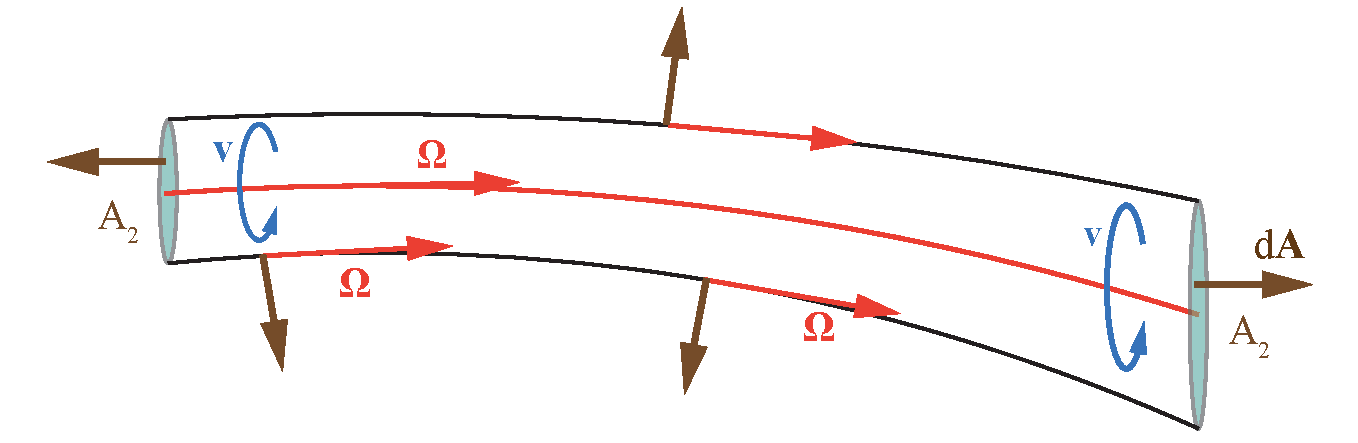
\includegraphics[width=\textwidth]{Wirbellinien}
  \caption[Veranschaulichung einer Wirbelr�hre]{Veranschaulichung einer
    Wirbelr�hre. Auf dem Mantel zeigt der Wirbelvektor parallel zur
    Oberfl�che. Er wird von Wirbellinien, die tangential an die Wirbelvektoren
    liegen, gebildet.}
    \label{abb:kontmech_Wirbelroehre}
\end{figure}


\subsection{Skalierungseigenschaften der Navier-Stokes-Gleichung}
\label{Skalierungseigenschaften!Navier-Stokes-Gleichung}

Wir haben gesehen, dass Str�mungen von vielen Faktoren abh�ngen. Oft untersucht
man jedoch technische Bauteile in Str�mungskan�len an verkleinerten Modellen.
Es ist m�glich, dabei zu Ergebnissen aus den Modellversuchen zu kommen, 
aus denen man direkt das Verhalten eines Systems bei realen Gr��enverh�ltnissen schlie�en kann.
Das liegt an den Skalierungseigenschaften der Navier-Stokes-Gleichung
\eqref{eq:kontmech_NavierStokesFrei}. Wir schreiben dazu die
Gleichung noch einmal auf,
\begin{equation*}
  \varrho \lk \lk \vec{v} \cdot \nablav \rk \vec{v} + \frac{\partial}
  {\partial t}\vec{v} \rk = \eta \, \Delta \vec{v} - \nablav p \; . \\
\end{equation*}
Um eine Skalierung der L�ngen durchf�hren zu k�nnen, f�hren wir eine
L�ngeneinheit $l$ so ein, dass wir in der Navier-Stokes-Gleichung nur
noch dimensionslose Ortsvariable stehen haben,
\begin{equation*}
  \vec{r} = l \, \tilde{\vec{r}} \, \qquad \nablav = \frac{1}{l} \tilde{\nablav}
  \; \quad \Delta = \frac{1}{l^2} \tilde{\Delta} \; .
\end{equation*}
Als weitere wichtige Gr��e geht die Str�mungsgeschwindigkeit ein. Auch f�r
diese f�hren wir mit der Geschwindigkeitseinheit $u$ �ber
\begin{equation*}
  \vec{v} = u \, \tilde{\vec{v}}
\end{equation*}
eine Skalierung ein. Aus diesen beiden folgt eine Zeiteinheit, die auch
auf Zeitableitungen anzuwenden ist,
\begin{equation*}
  t = \frac{l}{u} \, \tilde{t} \, \qquad \frac{\partial}{\partial t}
  = \frac{u}{l}\frac{\partial}{\partial \tilde{t}} \; .
\end{equation*}

Setzen wir alle diese Skalierungen ein, erhalten wir
\begin{equation*}
  \varrho \frac{u^2}{l} \lk \lk \tilde{\vec{v}} \cdot \tilde{\nablav} \rk
  \tilde{\vec{v}} + \frac{\partial}{\partial \tilde{t}} \tilde{\vec{v}} \rk
  = \frac{u}{l^2} \eta \, \tilde{\Delta} \tilde{\vec{v}} - \frac{1}{l}
  \tilde{\nablav} p \; , \\
\end{equation*}
was sich durch den Vorfaktor der linken Seite dividieren l�sst, sodass
wir
\begin{equation}
  \lk \tilde{\vec{v}} \cdot \tilde{\nablav} \rk \tilde{\vec{v}}
  + \frac{\partial}{\partial \tilde{t}} \tilde{\vec{v}} 
  = \frac{1}{u\,l\,\varrho} \eta \, \tilde{\Delta} \tilde{\vec{v}}
  - \tilde{\nablav} \frac{p}{\varrho\,u^2} \; \label{eq:kontmech_NavierStokesSkaliert01}
\end{equation}
erhalten.

Man erkennt also, dass man dasselbe Str�mungsverhalten erh�lt, wenn man die
\gls{reynoldszahl}\footnote{Osborne Reynolds (1842 -- 1912) war ein irisch-britischer Physiker. Nach ihm ist die Kennzahl zur Beurteilung viskoser Str�mungen und insbesondere deren �bergang zur Turbulenz benannt.}\indexp{Reynolds, Osborne}\index{Reynoldszahl}
\begin{equation}
  \mathrm{Re} = \frac{\varrho\,u\,l}{\eta}
\end{equation}
und den dimensionslosen Druck
\begin{equation}
  \tilde{p} = \frac{p}{\varrho\,u^2}
\end{equation}
konstant h�lt. In dieser Skalierung lautet die Navier-Stokes-Gleichung dann
\begin{equation}
  \lk \tilde{\vec{v}} \cdot \tilde{\nablav} \rk \tilde{\vec{v}}
  + \frac{\partial}{\partial \tilde{t}} \tilde{\vec{v}} 
  = \frac{1}{\mathrm{Re}} \, \tilde{\Delta} \tilde{\vec{v}}
  - \tilde{\nablav} \tilde{p} \; . \label{eq:kontmech_NavierStokesSkaliert02}
\end{equation}

�berschreitet die Reynolds-Zahl einen (problemabh�ngigen) kritischen Wert $\mathrm{Re}_\text{krit}$, wird eine bis dahin laminare Str�mung anf�llig gegen kleinste St�rungen und es findet ein �bergang von laminarer zu turbulenter Str�mung statt. F�r Experimente in der Hydrodynamik und Aerodynamik muss der Wert der Reynolds-Zahl von Original und verkleinerten Modell gleich sein, um ein �hnliches Str�mungsfeld zu erhalten. In der Literatur wird h�ufig ein Wert von $\mathrm{Re}_\text{krit} \approx 2300$ \cite{Schade1989, BergmannSchaefer1998} angegeben. 
Allerdings gibt die kritische Reynolds-Zahl nicht exakt den �bergang von einer laminaren zu einer turbulenten Str�mung an. H�ufig zerfallen Turbulenzen unterhalb der kritischen Reynolds-Zahl wieder schnell, insbesondere je kleiner die Reynolds-Zahl ist. Andererseits ist es in Experimenten gelungen, laminare Rohrstr�mungen mit Reynolds-Zahlen bis $\SI{50000}{}$ zu erzeugen, ohne dass dabei die Str�mung turbulent geworden ist \cite{Schade1989, BergmannSchaefer1998}. 




\clearpage
\section{Eigenschaften und Dynamik deformierbarer, fester K�rper}
\label{kap:kontmech_fest}\index{K�rper!elastische}\index{K�rper!deformierbare}

Bisher haben wir Fl�ssigkeiten und Gase als Beispiele f�r ein Kontinuum betrachtet. Doch wir ben�tigen auch
eine Beschreibung fester kontinuierlicher K�rper. Diese sind vor allem
durch ihr Verhalten bei Deformationen gekennzeichnet, das sich wesentlich von den Fluiden unterscheidet und das zur Beschreibung
ihrer Eigenschaften herangezogen wird. Diese Eigenschaften wollen wir zun�chst kl�ren,
bevor wir uns der Dynamik der Festk�rper-Kontinua widmen k�nnen.


\subsection{Eigenschaften deformierbarer K�rper}
\label{kap:kontmech_festEigenschaften}
\index{deformierbare K�rper!Eigenschaften}

Die Eigenschaften deformierbarer fester K�rper sind durch ihren (atomaren)
Aufbau gegeben. In einer einfachen klassischen Modellvorstellung k�nnen wir davon
ausgehen, dass alle Atomr�mpfe eines Festk�rpers sich so anordnen, dass
sich insgesamt und auch lokal ein energetisches (Potential-)Minimum ergibt. 
% im elektrostatischen Potential der Atome ein Minimum angenommen wird.
% Das elektrostatische Potentila ist ja bis hierher noch nicht eingef�ht.
Analog k�nnen wir in einer kontinuierlichen
Betrachtung modellieren, dass f�r eine bestimmte Konfiguration eines
materiellen Punkts des Kontinuums im Raum $\vec{r}_0$ ein Minimum des Potentials angenommen
wird. Wenn wir Deformationen betrachten, gehen wir von Abweichungen von
dieser idealen Lage der materiellen Punkte aus.

F�r kleine Abweichungen $\Delta \vec{r} = \vec{r} - \vec{r}_0$ entwickeln wir
das Potential in eine Potenzreihe um $\vec{r}_0$ (siehe auch \eqref{eq:bew_Schwingung_a} in \kap{bew_schwingung})
\begin{equation*}
  U(\vec{r}) = U(\vec{r}_0 + \D \vec{r}) = U(\vec{r}_0) + \nablav U(\vec{r}_0) \cdot \D \vec{r}
  + \frac{1}{2} \sum_{j,k}^3 \frac{\partial^2 U(\vec{r}_0)}{\partial x_j \,
    \partial x_k}\, \D x_j \, \D x_k + \dots \, ,
\end{equation*}
wobei oft nur die niedrigsten Ordnungen in Betracht gezogen werden m�ssen.
Die erste Ordnung verschwindet, da $\vec{r}_0$ ein Minimum darstellt,
wir erhalten also unter Benutzung der Einsteinschen Summenkonvention
\begin{equation*}
  U(\vec{r}) \approx \frac{1}{2} \, \frac{\partial^2 U(\vec{r}_0)}
  {\partial x_j \, \partial x_k}\, \D x_j \, \D x_k \; .
\end{equation*}
Das lineare Kraftgesetz ergibt sich in diesem Fall aus:
\begin{align}
  F_i(\vec{r}) &= \frac{1}{\d x_i} \, U(\vec{r}) \approx \frac{1}{2} \,
                  \frac{1}{\d x_i} \lek \frac{\partial^2 U(\vec{r}_0)} {\partial x_j \, \partial x_k}\, \stackrel{\downarrow}{\D x_j } \D x_k 
	                     +\frac{\partial^2 U(\vec{r}_0)} {\partial x_j \, \partial x_k}\,\D x_j \stackrel{\downarrow}{\D x_k }  \rek \notag \\
               &= \frac{1}{2} \lek \frac{\partial^2 U(\vec{r}_0)}{\partial x_j \,\partial x_k}\, \delta_{ij} \D x_k 
							                   + \frac{\partial^2 U(\vec{r}_0)}{\partial x_j \,\partial x_k}\, \delta_{ik} \D x_j \rek = \frac{\partial^2
  U(\vec{r}_0)} {\partial x_i \, \partial x_k}\, \Delta x_k \; . \label{eq:kontmech_kraefte_FK} 
\end{align}
Im Folgenden wollen wir verschiedene M�glichkeiten betrachten.

\subsubsection{Kontraktionen und Elastizit�tsmodul}
\label{kap:kontmech_festKontraktionen}
\index{Elastizit�tsmodul}

Als ersten Fall betrachten wir einen Festk�rper, der in eine Richtung
gedehnt wird und wollen die Kraftwirkung in genau diese Richtung wissen, siehe
\figref{kontmech_ElastTorsion}a. Wir interessieren uns also
f�r den Fall
\begin{equation}
  F_i = \frac{\partial^2 U(\vec{r}_0)}{\partial x_i \, \partial x_i}
  \, \Delta x_i \;,
  \label{eq:kontmech_Elastizitaetsmodul1}
\end{equation}
wobei wir von \eqref{eq:kontmech_kraefte_FK} zu \eqref{eq:kontmech_Elastizitaetsmodul1} zu kleinen Differenzgr��en $\Delta x_i $ �bergegangen sind. Dieser Fall tritt auf, wenn es keine Mischterme in den Ableitungen des Potentials
gibt. Es kann aber auch sein, dass ausschlie�lich $\Delta x_i \neq 0$.

\begin{figure}
  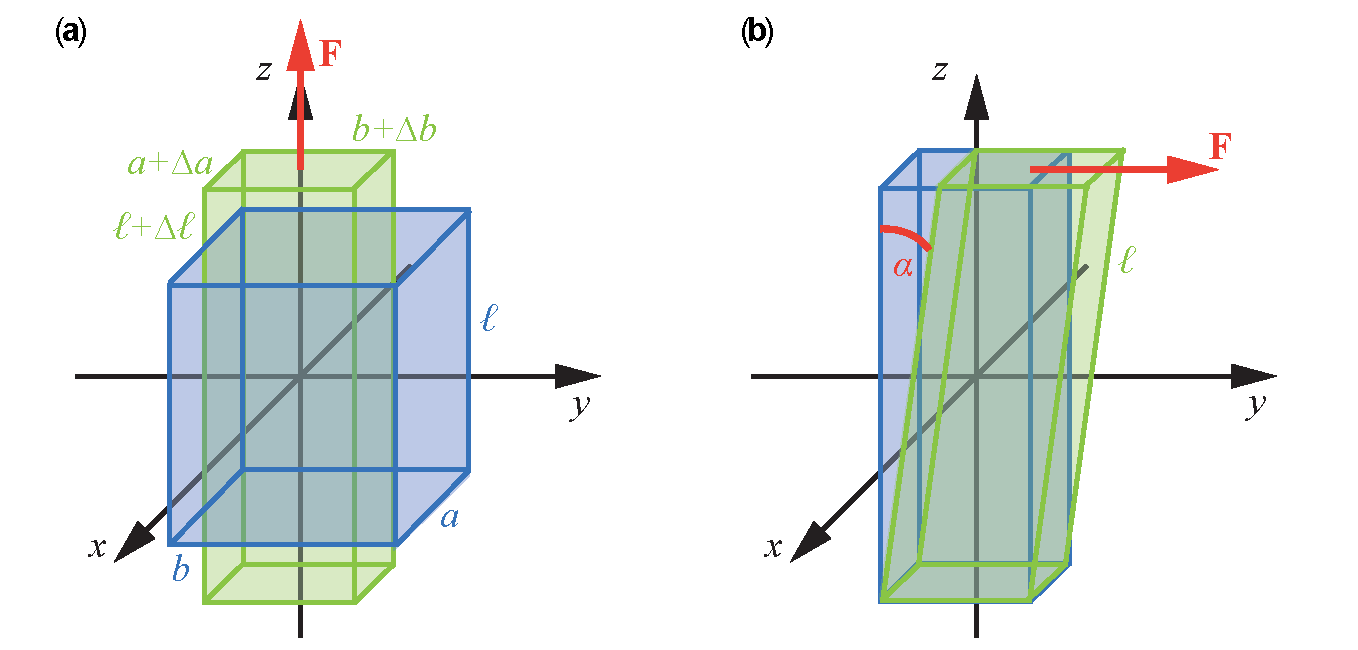
\includegraphics[width=\textwidth]{ElastTorsion.pdf}
  \caption[Zum Elastizit�tsmodul und Torsionsmodul]{Zum Elastizit�tsmodul und Torsionsmodul. \fa Darstellung einer
    Streckung mit der Zugkraft $\vec{F}$, die zur Definition des
    Elastizit�tsmoduls eingef�hrt wird. Dabei �ndern sich typischerweise auch
    die Ausdehnungen des K�rpers senkrecht zur Kraft. Die dazugeh�rigen
    Variablen $\Delta a$ und $\Delta b$ haben negative Werte. \fb Eine Scherung
    um den Winkel $\alpha$ f�hrt ebenfalls zu einem Widerstand, der durch die
    Kraft $\vec{F}$ �berwunden wird und �ber den sich das Torsionsmodul
    einf�hren l�sst.}
  \label{abb:kontmech_ElastTorsion}
\end{figure}

Mit dem Querschnitt $A$ des Elements des K�rpers, das verl�ngert wird, seiner
ungest�rten L�nge $\ell$ und der Verl�ngerung $\Delta \ell = \Delta x_i$
lasst sich Gleichung \eqref{eq:kontmech_Elastizitaetsmodul1} auf die Form
\begin{equation}
  F_i = \left ( \frac{\ell}{A} \frac{\partial^2 U(\vec{r}_0)}{\partial x_i
      \, \partial x_i} \right ) \, A \, \frac{\Delta \ell}{\ell}
  \label{eq:kontmech_Elastizitaetsmodul2}
\end{equation}
bringen. Mit dieser Form f�hrt man das \emph{\gls{Elastizitaetsmodul}}
\begin{equation}
  E = \frac{\ell}{A} \frac{\partial^2 U(\vec{r}_0)}{\partial x_i \,
    \partial x_i}
  \label{eq:kontmech_DefElastizitaetsmodul}
\end{equation}
ein und schreibt
\begin{equation}
  F = E \, A \, \frac{\Delta \ell}{\ell}
  \label{eq:kontmech_Elastizitaetsmodul3}
\end{equation}
beziehungsweise f�r die \emph{Zugspannung} $\sigma = F/A$
\begin{equation}
  \sigma = E \, \frac{\Delta \ell}{\ell} \; .
  \label{eq:kontmech_Elastizitaetsmodul4}
\end{equation}

�blicherweise �ndert sich jedoch nicht allein die L�nge des K�rpers. Es kommt
entlang der beiden Richtungen der Fl�che $A$ im Normalfall zu einer
Kontraktion. Um die Verk�rzung einer Richtung in der Fl�che zur Verl�ngerung
in der Richtung senkrecht dazu in Relation zu setzen (vgl.
\figref{kontmech_ElastTorsion}a), wird die \emph{\gls{Poissonzahl}}\footnote{Sim�on Denis Poisson (1781--1840 in Paris) war ein franz�sischer Physiker und Mathematiker. Er war Sch�ler von Laplace und besch�ftigte sich vor allem mit der Theorie der Wellen in der Akustik, der Elastizit�ts- und W�rmelehre, sowie �ber die Potentialtheorie der Elektrostatik. Als Mathematiker arbeitete Poisson vor allem auf den Gebietender Differentialgeometrie, der Infinitesimal- und Wahrscheinlichkeitsrechnung. Mehrere mathematische Begriffe sind mit seinem Namen verbunden. Er war sehr produktiv und ver�ffentlichte insgesamt �ber 300 Arbeiten.}\indexp{Poisson, Sim�on Denis}\index{Poissonzahl}
\begin{equation}
  \nu = -\frac{\Delta a\, /\, a}{\Delta \ell\, /\, \ell} =
  -\frac{\Delta b\, /\, b}{\Delta \ell\, /\, \ell}
  \label{eq:kontmech_Poissonzahl}
\end{equation}
eingef�hrt\footnote{Die Variablen $\Delta a$ und $\Delta b$, die die Stauchung
  in den beiden Richtungen senkrecht zur Streckung beschreiben, haben hier
  negative Werte. Die Poissonzahl ist so definiert, dass sie selbst positiv
  ist.}.
Typische Werte der Poissonzahl liegen f�r Metalle zwischen 0.2 und 0.4, f�r Beton bei 0.2 
und f�r Faserverbundstoffe bei kleiner 0.05.
Damit k�nnen wir nun die Deformation des gesamten Volumens betrachten. Diese
ergibt sich z.B. f�r eine rechteckige Fl�che zu
\begin{equation*}
  \Delta V = (a + \Delta a )(b + \Delta b )(\ell + \Delta \ell) - ab\ell \; ,
\end{equation*}
was f�r typischerweise kleine �nderungen in linearer N�herung zu
\begin{equation*}
  \Delta V = a b \Delta \ell + a \Delta b \ell + \Delta a b \ell
\end{equation*}
angegeben werden kann. F�r das Verh�ltnis findet man damit
\begin{equation*}
  \frac{\Delta V}{V} = \frac{\Delta \ell}{\ell} + \frac{\Delta a}{a} +
  \frac{\Delta b}{b} = \frac{\Delta \ell}{\ell} - \nu \frac{\Delta \ell}{\ell}
  -\nu \frac{\Delta \ell}{\ell}
  = ( 1 - 2 \nu )  \frac{\Delta \ell}{\ell} \; ,
\end{equation*}
was nun auch mit der angelegten Zugspannung verkn�pft werden kann,
\begin{equation*}
  \frac{\Delta V}{V} = \frac{\sigma}{E} ( 1 - 2 \nu ) \; .
\end{equation*}


\subsubsection{Inelastische K�rper}
\label{kap:kontmech_festinelastisch}
\index{deformierbare K�rper!inelastische}

Die bisherige Betrachtung ging davon aus, dass die Kraft allein durch die zweite
Ableitungen des Potentials ausgedr�ckt werden kann, also eine lineare Zunahme
der Kraft mit der Streckung oder Stauchung vorliegt. Dies ist der Fall
des Hookschen Gesetzes\index{Hooksches Gesetz|textbf}\indexp{Hooke, Robert}, das wir schon aus \kap{bew_newton_axioms}
kennen. Dies ist jedoch nicht beliebig der Fall, sondern gilt nur bis zur
\emph{Proportionalit�tsgrenze}\index{Proportionalit�tsgrenze!elastische K�rper}
im jeweiligen Material. Ist diese �berschritten, dehnt sich der K�rper bei
zunehmender Kraft st�rker aus, als es innerhalb der Proportionalit�tsgrenze
der Fall w�re.

Plastische Verformungen, die durch innere Umlagerungseffekte im Material
ausgel�st werden, treten bei noch h�heren Streckungen oder Kontraktionen auf.
Diese sorgen daf�r, dass das Material auch bei komplettem Verschwinden der
ausdehnenden Kraft nicht in seine urspr�ngliche Gestalt zur�ckkehrt.

Jedoch k�nnen auch innerhalb des Elastizit�tsbereichs zumindest kurzzeitige
Streckungen oder Stauchungen zur�ck bleiben, wenn keine Kraft mehr auf den
K�rper einwirkt. 
%Dies ist besonders bei sehr schnell einwirkenden Kr�ften der Fall.
In diesem Fall erh�lt man eine Hystereseschleife\index{Hysterese!elastische K�rper},
siehe \figref{kontmech_HystereseschleifeKompression}. Nach der Streckung des
K�rpers bis zum Punkt A durch die Zugspannung $\sigma_\text{A}$
und anschlie�ender Entspannung kehrt der K�rper nicht in den Ursprung zur�ck,
sondern es verbleibt eine restliche Streckung, die durch den Punkt C markiert
ist. Ein Druck bis zu $\sigma_\text{B}$ bewirkt eine Kompression bis zum
Punkt B. Entspannt man auch hier wieder bleibt die Stauchung, die durch den
Punkt D markiert ist, �brig.

\begin{figure}
  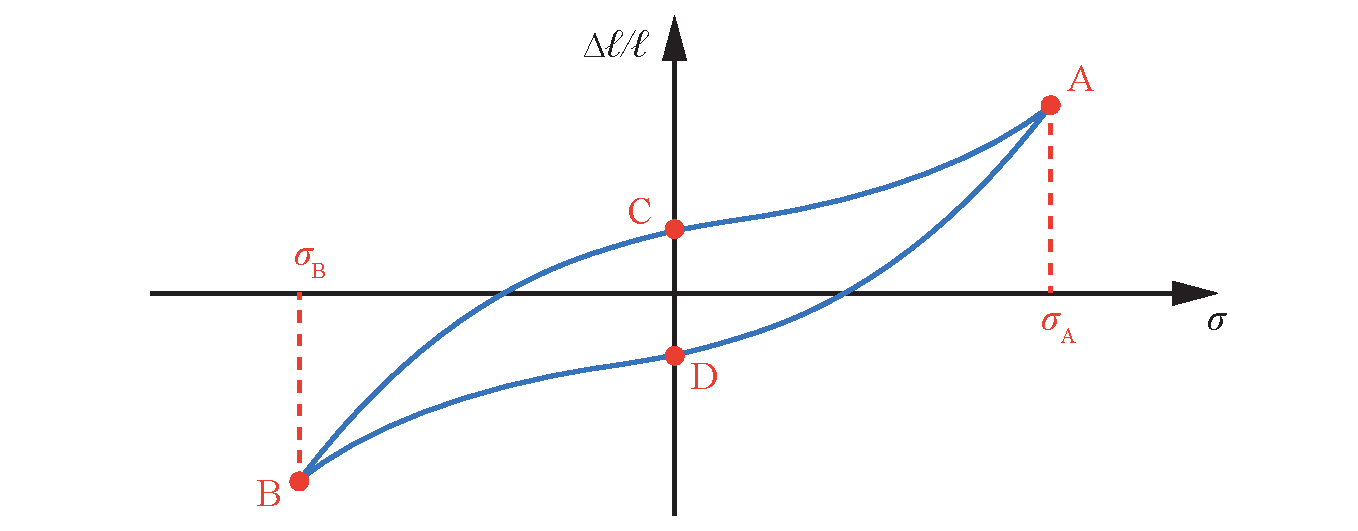
\includegraphics[width=\textwidth] {Spannungshysterese.pdf}
  \caption[Hystereseschleife\index{Hystereseschleife} bei Zugspannungen]{Mechanische
    Hystereseschleife bei der Kompression und Expansion eines elastischen
    K�rpers durch eine Zugspannung.}
  \label{abb:kontmech_HystereseschleifeKompression}
\end{figure}


\subsubsection{Scherungen und Torsionsmodul}
\label{kap:kontmech_festtorsion}
\index{Torsionsmodul|textbf}\index{Schubmodul|textbf}\index{Scherung}

Greift eine Kraft nicht senkrecht zur Fl�che eine K�rpers, sondern tangential
an, so f�hrt sie zu einer Scherung (siehe
\figref{kontmech_ElastTorsion}b). Der K�rper wird auch gegen diese
Bewegung einen Widerstand leisten, der durch eine Tangentialkraft $F_t$
�berwunden werden muss. Diese l�sst sich analog zu Gleichung
\eqref{eq:kontmech_Elastizitaetsmodul2} durch das innere Potential des
Festk�rpers ausdr�cken,
\begin{equation}
  F_t = \left ( \frac{1}{A} \frac{\partial^2 U(\vec{r}_0)}{\partial x_j
      \, \partial x_j} \frac{\partial \, (\Delta x_j)}{\partial \alpha} \right )
  \, A \, \alpha \; ,
  \label{eq:kontmech_Torsionsmodul1}
\end{equation}
wobei $\alpha$ der Winkel ist, um den die Scherung erfolgt. �hnlich
zum Elastizit�tsmoduls $E$ findet man f�r den Term in der Klammer
\begin{equation}
  G = \frac{1}{A} \frac{\partial^2 U(\vec{r}_0)}{\partial x_j
      \, \partial x_j} \frac{\partial (\Delta x_j)}{\partial \alpha} \; ,
  \label{eq:kontmech_Torsionsmodul2}
\end{equation}
der den Namen \emph{Torsionsmodul} oder \emph{\gls{Schubmodul}} erh�lt. �hnlich
der Zugspannung $\sigma$ l�sst sich unter Verwendung des Torsionsmoduls
die Scherspannung
\begin{equation}
  \tau = \frac{F_t}{A} = G \alpha
  \label{eq:kontmech_Torsionsmodul3}
\end{equation}
bilden.

F�r kleine Winkel kann man die Form von $G$ der von $E$ anpassen. Gehen wir davon
aus, dass $\alpha$ klein ist und somit $\sin \alpha \approx \alpha$ gilt, so
erhalten wir mit $\Delta x_j = \ell\, \sin \alpha \approx \ell\, \alpha$
\begin{equation*}
  \frac{\partial\, \Delta x_j}{\partial \alpha} = \frac{\partial \ell \alpha}
  {\partial \alpha} = \ell
\end{equation*}
und somit nimmt das Torsionsmodul die Gestalt
\begin{equation*}
  G = \frac{\ell}{A} \frac{\partial^2 U(\vec{r}_0)}{\partial x_j
    \, \partial x_j} 
\end{equation*}
an, die rein formal nicht mehr von der von $\ell$ zu unterscheiden ist. Ganz
analog findet man dann auch f�r die Tangentialkraft die zu
\eqref{eq:kontmech_Elastizitaetsmodul2} identische Form
\begin{equation}
  F_t = \lk \frac{\ell}{A} \frac{\partial^2 U(\vec{r}_0)}{\partial x_j
      \, \partial x_j} \rk \, A \, \frac{\Delta x_j}{\ell} \; .
  \label{eq:kontmech_Torsionsmodul4}
\end{equation}
Dabei muss man jedoch fest im Blick behalten, in welche Richtung die Kr�fte
angreifen. In der Komponentendarstellung, die wir gew�hlt haben, kommt nicht
zum Ausdruck, dass die Kraft tangential zur Fl�che angreift. Diese Tatsache
bildet jedoch den wesentlichen Unterschied zwischen Elastizit�ts- und Torsionsmodul.

\subsection{Dynamik deformierbarer K�rper}
\label{kap:kontmech_festDynamik}
\index{deformierbare K�rper!Dynamik}


\subsubsection{Lagrange-Formalismus f�r kontinuierliche K�rper}
\label{kap:kontmech_festLagrange}%
\index{Lagrange-Gleichung!kontinuierliche K�rper}%
%\index{schwingende Saite}
\index{Saite!schwingende|textbf}

Der Lagrange-Formalismus eignet sich gut, um dynamische Gleichungen auch f�r
elastische deformierbare K�rper aufzustellen. Um diesen motivieren zu k�nnen,
beginnen wir mit dem einfachen Beispiel einer schwingenden Saite. Diese
stellen wir uns zun�chst als eine Kette von Massepunkten identischer Masse $m$ vor,
die durch Federn der Ruhel�nge $d$ und der Federrichtgr��e $k_\text{F}$ miteinander
verbunden sind, siehe Abbildung \ref{abb:kontmech_SaiteMassepunkte}. Sp�ter
werden wir den Abstand $d$ zwischen den Massepunkten gegen Null gehen lassen,
um den �bergang zum kontinuierlichen System zu vollziehen.

\begin{figure}
  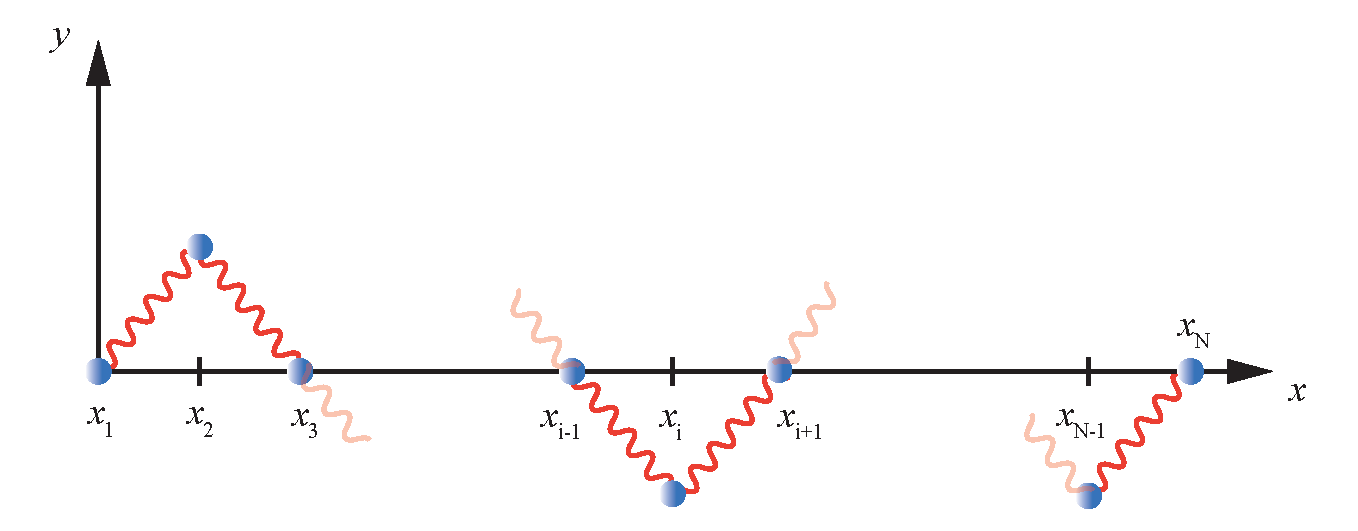
\includegraphics[width=\textwidth] {SchwingSaiteModell.pdf}
  \caption[Modell aus Massepunkten f�r eine schwingende Saite]{Eine schwingende
    Saite wird durch $N$ Massepunkte gleicher Masse $m_i=m$, die durch Federn verbunden
    sind, modelliert. Die Massen  $m_i$ f�r $i=0$ und $i=N-1$ sollen unbeweglich am
    Rand sein.}
    \label{abb:kontmech_SaiteMassepunkte}
\end{figure}

Entsprechend \kap{bew_Lagrange_II} m�ssen wir f�r die
Lagrange-Gleichungen zweiter Art zun�chst die kinetische Energie und das
Potential aufstellen. Das Modell setzt voraus, dass die Koordinaten $x_i$
fest bleiben und sich die Massepunkte nur in Richtung der $y_i$ bewegen k�nnen.
Damit ergibt sich f�r die kinetische Energie
\begin{equation*}
  T(\{\dot{y}_i\}) = \sum_{i=1}^N T_i = \sum_{i=1}^N \frac{m}{2} \,\dot{y}_i^2 \; .
\end{equation*}
F�r das Potential, das sich aus der angenommenen Feder zwischen den
Massepunkten $i-1$ und $i$ ergibt, gilt mit der Annahme, dass wir die
Abstands�nderungen in $x$-Richtung vernachl�ssigen k�nnen, weil diese Abst�nde als starr
angenommen werden und somit nicht zur Bewegung beitragen:
\begin{equation*}
  U(\{y_i\}) = \sum_{n=2}^{N} \frac{k_\text{F}}{2} (y_i - y_{i-1})^2 \; .
\end{equation*}
Somit l�sst sich die Lagrange-Funktion aufstellen zu
\begin{equation}
  \mathcal{L}(\{y_i\},\{\dot{y}_i\}) = T(\{\dot{y}_i\}) - U(\{y_i\})
  = \sum_{i=1}^N \frac{m}{2} \dot{y}_i^2
  - \sum_{i=2}^{N} \frac{k_\text{F}}{2} (y_i - y_{i-1})^2 \; .
  \label{kontmech_SaiteLagrangePunkte}
\end{equation}
Mit diesem Ansatz k�nnen wir zum kontinuierlichen System �bergehen. Dazu
verwenden wir die kontinuierliche Variable $x$ anstatt des Z�hlindex $i$
und schreiben f�r die Koordinaten
\begin{equation*}
  y_i \to y(x)\;, \qquad y_{i} - y_{i-1} \to \D x \, \left . \frac{\D y}{\D x} \right |_x  
\end{equation*}
und verwenden die (lineare) Dichte $\varrho_\mathrm{L}$ in $\SI{}{\kg\per\metre}$ statt der Masse $m$ sowie die Zugkraft\footnote{Diese entspricht hier in der eindimensionalen Betrachtung dem \gls{Elastizitaetsmodul} im mehrdimensionalen Fall.} $\Phi$ in $\SI{}{\N}$ statt der Federrichtgr��e $k_\text{F}$:
\begin{equation*}
  m = \varrho_\text{L} d \; , \qquad k_\text{F} = \frac{\Phi}{d} \; .
\end{equation*}
Dies f�hrt mit Gleichung \eqref{kontmech_SaiteLagrangePunkte} auf die
Lagrange-Funktion
\begin{align*}
  \mathcal{L} &= \sum_{i=1}^N \frac{\varrho_\text{L} d}{2} \lk \frac{\partial y(x,t)}
                {\partial t} \rk^2
                - \sum_{i=2}^{N} \frac{\Phi}{2 d} \lk \frac{\partial y(x,t)}
                {\partial x}
                \rk^2 d^2 \\
              &= \frac{\varrho d}{2} \left [
                \sum_{i=1}^N \lk \frac{\partial y(x,t)}{\partial t} \rk^2
                - \sum_{i=2}^{N} \frac{\Phi}{\varrho_\text{L}} \lk
                \frac{\partial y(x,t)}{\partial x} \rk^2 \right ] \; .
\end{align*}
Der Grenz�bergang zum kontinuierlichen System wird durch
\begin{equation*}
  d \sum_i \to \int \D x
\end{equation*}
vollzogen, was auf die kontinuierliche Lagrange-Funktion
\begin{equation}
   \mathcal{L} = \int \D x \; \frac{\varrho_\text{L}}{2} \left [
    \lk \frac{\partial y(x,t)}{\partial t} \rk^2 - \frac{\Phi}{\varrho_\text{L}}
    \lk \frac{\partial y(x,t)}{\partial x} \rk^2 \right ]
  \label{eq:kontmech_SaiteLagrangeFunktion}
\end{equation}
f�hrt.

In der Lagrange-Funktion \eqref{eq:kontmech_SaiteLagrangeFunktion} tritt die
\emph{Lagrange-Dichte}\index{Lagrange-Dichte|textbf}
\begin{equation}
  L \lk \frac{\partial y}{\partial t}, \frac{\partial y}{\partial x} \rk
  = \frac{\varrho_\text{L}}{2} \left [ \lk \frac{\partial y(x,t)}{\partial t} \rk^2
    - \frac{\Phi}{\varrho_\text{L}} \lk \frac{\partial y(x,t)}{\partial x} \rk^2
  \right ]
  \label{eq:kontmech_LagrangedichteSaite}
\end{equation}
auf, die wir heranziehen k�nnen, um die dynamischen Gleichungen zu gewinnen.

In \kap{bew_Lagrange_II} wurden die Lagrange-Gleichungen zweiter
Art aus denen erster Art durch den �bergang auf generalisierte Koordinaten
gewonnen. Man kann zeigen, dass sich dieselben Gleichungen aus einer
�quivalenten Forderung erhalten lassen. Die klassischen Bahnen sind n�mlich diejenigen, die
das \gls{Wirkungsfunktional}\index{Wirkungsfunktional}
\begin{equation*}
  S = \int \mathcal{L}(\{q_i\},\{\dot{q}_i\},t)\, \D t
\end{equation*}
extremal machen (siehe \cite{Schmutzer2005, Kuypers2012, Bartelmann2015}), f�r die also gilt
\begin{equation*}
  \delta S = \int \mathcal{L}(\{q_i+\delta q_i\},\{\dot{q}_i+\delta\dot{q}_i\}
  ,t)  \D t - \int \mathcal{L}(\{q_i\},\{\dot{q}_i\},t)\, \D t = 0  \; ,
\end{equation*}
wobei $\delta q_i(t)$ eine Variation der klassischen Bahn ist, die nur die
Randbedingung erf�llen muss, dass sie am Anfang und Ende der Bahn
verschwindet, also $\delta q_i(t_\mathrm{Start})=\delta q_i(t_\mathrm{Ende})=0$.
Dieselbe Forderung k�nnen wir an die Lagrange-Funktion\index{Lagrange-Funktion}
\eqref{eq:kontmech_SaiteLagrangeFunktion} der schwingenden Saite stellen. Dazu
f�hren wir die Variation der Auslenkung
\begin{equation*}
  y(x,t) = y(x,t) + \delta y(x,t)
\end{equation*}
ein und stellen das Wirkungsfunktional
\begin{equation}
  S = \int \mathcal{L}\,\D t = \int \D t \int \D x\,
  L \lk \frac{\partial y}{\partial t}, \frac{\partial y}{\partial x} \rk
\end{equation}
auf. Damit berechnen wir die Variation der Wirkung
\begin{align*}
  \delta S &= \int \D t \int \D x\,
             L \lk \frac{\partial y}{\partial t} + \frac{\partial \delta y}
             {\partial t},
             \frac{\partial y}{\partial x} + \frac{\partial \delta y}
             {\partial x}  \rk  - \int \D t \int \D x\,
             L \lk \frac{\partial y}{\partial t}, \frac{\partial y}
             {\partial x} \rk \; ,\\
  \intertext{was in linearer N�herung}
  \delta S &= \int \D t \int \D x\, \left [
             \frac{\partial L}{\partial \lk \frac{\partial y}{\partial t} \rk}
             \frac{\partial \delta y}{\partial t}
             + \frac{\partial L}{\partial \lk \frac{\partial y}{\partial x} \rk}
             \frac{\partial \delta y}{\partial x} \right ] \\
  \intertext{ergibt und mit partieller Integration auf}
  \delta S &= \int \D t \int \D x\, \left [
             -\frac{\partial}{\partial t} \frac{\partial L}
             {\partial \lk \frac{\partial y}{\partial t} \rk}
             - \frac{\partial}{\partial x} \frac{\partial L}
             {\partial \lk \frac{\partial y}{\partial x} \rk} \right ] \delta y
\end{align*}
f�hrt. Da die Variation $\delta y$ bis auf die Forderung nach verschwindenden Ver�nderungen an den Randpunkten
beliebig ist, fordert dies auch
\begin{equation}
  -\frac{\partial}{\partial t} \frac{\partial L}
  {\partial \lk \frac{\partial y}{\partial t} \rk}
  - \frac{\partial}{\partial x} \frac{\partial L}
  {\partial \lk \frac{\partial y}{\partial x} \rk} = 0
\end{equation}
und mit der Lagrange-Dichte\index{Lagrange-Dichte} der schwingenden Saite \eqref{eq:kontmech_LagrangedichteSaite}
erhalten wir schlie�lich:
\begin{equation}
  \varrho_\text{L} \frac{\partial^2 y(x,t)}{\partial t^2}
  - \Phi \frac{\partial^2 y(x,t)}{\partial x^2} = 0 \; .
  \label{eq:kontmech_PDGLSaite}
\end{equation}
Dies ist die gesuchte dynamische Gleichung f�r die schwingende Saite. Dividiert man beide Seiten von \eqref{eq:kontmech_PDGLSaite} durch die als konstant angenommene Querschnittsfl�che $A$, dann erh�lt man mit dem \gls{Elastizitaetsmodul} $E = \Phi / A$ die \emph{Wellengleichung}\index{Wellengleichung} f�r die schwingende Saite in der �blichen Darstellung mit der Volumendichte $\varrho$:
\begin{equation}
  \varrho \frac{\partial^2 y(x,t)}{\partial t^2}
  - E \frac{\partial^2 y(x,t)}{\partial x^2} = 0 \; .
  \label{eq:kontmech_PDGLSaite2}
\end{equation}


\newpage
%BEISPIEL %%%%%%%%%%%%%%%%%%%%%%%%%%%%%%%%%%%%%%%%%%%%%%%%%%%%%%%%%%%%%%%%%%%%%%%%%%%%%%%%%%
\begin{example}{Analytische L�sungen f�r die schwingende Saite}
\label{bsp:kontmech_schwingendeSaite}\index{Saite!schwingende}
\smallskip

Die Wellengleichung \eqref{eq:kontmech_PDGLSaite2} hat sehr
viele verschiedene L�sungen, die meist durch Randbedingungen eingeschr�nkt
sind. Wir wollen uns hier auf zwei L�sungstypen beschr�nken.

Zun�chst betrachten wir L�sungen, die wir mit dem Produktansatz
\begin{equation*}
  y(t,x) = a(t)\,b(x) 
\end{equation*}
finden. Setzt man diesen in \eqref{eq:kontmech_PDGLSaite2} ein, k�nnen wir
dies auf die Form
\begin{equation*}
  \frac{1}{a(t)} \frac{\partial^2 a(t)}{\partial t^2} = \frac{E}{\varrho}
  \frac{1}{b(x)} \frac{\partial^2 b(x)}{\partial x^2} = C
\end{equation*}
bringen, wobei $C$ eine Konstante sein muss, da eine Seite nur von $t$, die
andere nur von $y$ abh�ngt. Dies erm�glicht uns, die beiden separierten
Differentialgleichungen getrennt zu l�sen. So finden wir \zb sehr einfach
die L�sungen
\begin{align*}
  a(t) &= \alpha_1 \mathrm{e}^{\sqrt{C}t} + \alpha_2 \mathrm{e}^{-\sqrt{C}t}
         \; , \\
  b(x) &= \beta_1 \mathrm{e}^{\sqrt{\frac{\varrho}{E} C}x}
         + \beta_2 \mathrm{e}^{-\sqrt{\frac{\varrho}{E} C}x} \; .
\end{align*}
Interessant f�r das Verhalten einer schwingenden Saite sind dabei vor allem
L�sungen, die nicht exponentiell anwachsen. Diese erhalten wir f�r ein negatives
$C$ und wir setzen nun
\begin{equation*}
  \sqrt{C} = \im \omega \; , \qquad \sqrt{\frac{\varrho}{E} C} = \im k
  \; ,
\end{equation*}
womit wir 
\begin{align*}
  a(t) &= \alpha_1 \mathrm{e}^{\im \omega t} + \alpha_2
         \mathrm{e}^{-\im \omega t} \; , \\
  b(x) &= \beta_1 \mathrm{e}^{\im k x} + \beta_2 \mathrm{e}^{-\im k x} 
\end{align*}
beziehungsweise
\begin{equation*}
  y(t,x) = \left \{ \alpha_1 \mathrm{e}^{\im \omega t} + \alpha_2
    \mathrm{e}^{-\im \omega t} \right \} \left \{ \beta_1 \mathrm{e}^{\im k x}
    + \beta_2 \mathrm{e}^{-\im k x}  \right \}
\end{equation*}
erhalten. Dies sind stehende Wellen, bei denen periodische r�umliche Strukturen
unabh�ngig vom Zeitverlauf bestehen. Der Zeitverlauf �ndert allein die Gr��e
Auslenkungen, nicht aber ihre Position entlang der Saite. Leichter sichtbar wird das f�r den Spezialfall $\alpha_1 = \alpha_2
= \alpha/2$, $\beta_1 = \beta_2 = \beta/2$, was auf die L�sung
\begin{equation*}
  y(t,x) = \alpha \beta \cos(\omega t) \cos(k x) 
\end{equation*}
f�hrt. Graphische Darstellungen finden sich in Beispiel
\ref{bsp:kontmech_finiteDiffSaite}, in dem wir dieses System numerisch mit der
Methode der finiten Differenzen l�sen werden.

Einen zweiten Typ von L�sungen, den wir betrachten wollen, sind fortlaufende
Wellen, die eine nahezu beliebige funktionale Form haben d�rfen. Der
Ansatz
\begin{equation*}
  y(t,x) = f(\omega t \pm kx)
\end{equation*}
mit $k$ als Wellenzahl und $\omega$ als Kreisfrequenz l�st ganz allgemein, wie man durch Einsetzen erkennt,
\begin{equation*}
  \varrho \omega^2 f''(\omega t \pm kx) = E k^2 f''(\omega t \pm kx) \; ,
\end{equation*}
die Differentialgleichung, falls die \gls{Dispersionsrelation} \index{Dispersionsrelation} 
\begin{equation}
  \omega = \sqrt{\frac{E}{\varrho}}\,k
  \label{eq:kontmech_DispersionsRel}
\end{equation}
erf�llt ist. F�r eine beidseitig eingespannte Saite verbieten sich jedoch solche L�sungen wegen der Randbedingungen.
Da die
Differentialgleichung linear ist, sind jederzeit beliebige �berlagerungen von L�sungen der beidseitig eingespannte Saite m�glich,
die in der Summe sich als ausbreitende Wellen auf der Saite interpretieren lassen. Beispiele werden
wir in \probref{kontmech_WelleSaite} untersuchen.
\end{example}

%BEISPIEL %%%%%%%%%%%%%%%%%%%%%%%%%%%%%%%%%%%%%%%%%%%%%%%%%%%%%%%%%%%%%%%%%%%%%%%%%%%%%%%%%%


\subsubsection{Numerisches L�sungsverfahren �ber finite Differenzen}
\label{kap:kontemch_finiteDifferenzen}
\index{Finite Differenzen Methode}\index{Differenzen!finite}\index{Finite Differenzen Methode|textbf}

Lineare \emph{\gls{PDGL}en}\index{Differentialgleichung!partielle} (PDGL) der Form
\begin{equation}
  \left ( \sum_i a_i \frac{\partial^2}{\partial x_i^2} +
    \sum_i b_i \frac{\partial}{\partial x_i} + c \right )
  f(\vec{x}) + d = 0 \; ,   \label{eq:kontmech_GrundformPDGL1}
\end{equation}
zu denen auch die Differentialgleichung \eqref{eq:kontmech_PDGLSaite} der
schwingenden Saite geh�rt, lassen sich numerisch mit finiten Differenzen
l�sen. Wir k�nnen das hier nicht vollst�ndig einf�hren, wollen aber kurz die
Idee der L�sungsmethode vermitteln und verweisen auf das entsprechende Kapitel
im L�sungsteil \bzw auf die Literatur \cite{Otto2019, Fischer2014, Riley2006,
  Andrews2003}.
Wir beschr�nken uns auf den Fall einer PDGL 2. Ordnung mit zwei Variablen
($x_1 =x\,,\,\,x_2=t$), so dass aus \eqref{eq:kontmech_GrundformPDGL1} 
\begin{align}
  \lk a_{11} \frac{\partial^2}{\partial x^2} + a_{12} \frac{\partial^2}{\partial x\,\partial t} + a_{21} \frac{\partial^2}{\partial t\,\partial x } + a_{22} \frac{\partial^2}{\partial t^2} 
   + b_1 \frac{\partial}{\partial x} + b_2 \frac{\partial}{\partial t} + c \rk \,f(x,t)\nonumber \\
	&~~+ d = 0    \label{eq:kontmech_GrundformPDGL2}
\end{align}
wird.\\
Definiert man die Diskriminante
	\[\mathcal{D} = a_{11}\,a_{22} - \frac{a_{12}\,a_{21}}{4} \,,\]
dann unterscheidet man bei \eqref{eq:kontmech_GrundformPDGL2} verschiedene Typen:
Gilt $\mathcal{D}(x,t) > 0$, so hei�t die PDGL elliptisch im Punkt $(x,t)$, 
f�r $\mathcal{D}(x,t) = 0$ ist die PDGL parabolisch im Punkt $(x,t)$, 
und gilt $\mathcal{D}(x,t) <0$, so haben wir im Punkt $(x,t)$ eine hyperbolische PDGL vorliegen\footnote{Der Ursprung der Bezeichnungen elliptisch, parabolisch und hyperbolisch ergibt sich aus der Theorie der Kegelschnitte. Die allgemeine Kegelschnittgleichung $a_{11}\,x^{2}+a_{12}\,x\,y+a_{22}\,y^{2}+b_1\,x+b_2\,y+c=0$ 
ist von der Struktur her �hnlich aufgebaut wie die lineare partielle Differentialgleichung 2. Ordnung \eqref{eq:kontmech_GrundformPDGL2}.}.
Man findet unterschiedliche L�sungsprogramme f�r die einzelnen Typen. 
Die Wellengleichung als dynamische Gleichung f�r die schwingende Saite ist offensichtlich vom hyperbolischen Typus, denn es gilt $\mathcal{D}(x,t) = -\varrho E <0$.

Die L�sungsmethode der finiten Differenzen f�r diesen Fall baut nun darauf auf, dass man
die gesuchte Funktion $f(x,t)$ auf Gitterpunkten
\begin{equation*}
  (x = x_i \,, t = t_l)
\end{equation*}
definiert und damit das Differentialgleichungssystem diskretisiert. Man
bestimmt in der L�sung also die Daten $f(x_i,t_l)$ f�r alle
Indexkombinationen.

Dazu m�ssen nat�rlich auch die Ableitungen diskretisiert werden. Dies gelingt
zum Beispiel f�r ein (eindimensionales) Gitter aus �quidistanten Schritten $x_i = x_0 + i\,$
durch
\begin{subequations}
  \begin{align}
    \frac{\partial f(x_i)}{\partial x_i} &= \frac{f(x_{i+1}) - f(x_{i-1})}
                                           {2\Delta x}  \; ,
    \label{eq:kontmech_Diskretisierung1} \\
    \frac{\partial^2 f(x_i)}{\partial x_i^2} &= \frac{f(x_{i+1}) + f(x_{i-1})
                                               -2 f(x_i)}{\Delta x^2}
    \label{eq:kontmech_Diskretisierung2} \; ,
\end{align}
\end{subequations}
was nat�rlich analog f�r alle anderen Variablen gilt, w�hrend diese f�r
die $x$-Ableitungen festgehalten werden. Hier muss man nur
bedenken, dass die Randpunkte gesondert behandelt werden m�ssen, da die
Ableitungen symmetrisch aufgebaut sind. Bei unserer PDGL haben wir sogenannte 
Dirichlet\footnote{Dirichlet (1805�-1859) war ein deutscher Mathematiker, der haupts�chlich auf den Gebieten der Analysis und der Zahlentheorie t�tig war.}\indexp{Dirichlet, Peter Gustav Lejeune}-Randbedingungen\index{Randbedingungen!Dirichletsche}\footnote{Die Dirichlet-Randbedingung ist in der Mathematik eine Randbedingung, bei der die Ableitungen einer L�sung nur innerhalb der Dom�nengrenze angewendet wird.} vorliegen, die wir dadurch definieren, dass die Randwerte, \zb
$x_0,\, t_0$ und $x_{N+1},\, t_{N+1}$, auf einen festen Wert gesetzt werden,
\dh die Randpunkte werden im L�sungsverfahren nicht ge�ndert.

Prinzipiell kann man damit das Differentialgleichungssystem auf die 
Form einer Matrixgleichung f�r ein lineares Gleichungssystem
\begin{equation*}
  \mathbb{M} \,\vec{f} = \vec{0}
\end{equation*}
bringen (siehe auch \cite{Fischer2014}). Man sucht also f�r dieses lineare
Gleichungssystem den L�sungsvektor $\vec{f}$. Dieses Verfahren wird jedoch in
seiner Allgemeinheit relativ selten verwendet, da es sehr aufwendig ist.

In der Physik versucht man meist zu bestimmen, wie sich eine Bewegung K�rpers/Objektes
wie der schwingenden Saite in der Zeit ver�ndert. In diesem Fall
stellt man eine Iterationsgleichung f�r die Zeitschritte auf. Wie das
funktioniert, l�sst sich am einfachsten an einem Beispiel erkl�ren. Daf�r
greifen wir wieder auf die schwingende Saite zur�ck.

% BEISPIEL %%%%%%%%%%%%%%%%%%%%%%%%%%%%%%%%%%%%%%%%%%%%%%%%%%%%%%%%%%%%%%%%%%%%%%%%%%%%%%%%%%
\begin{example}{Numerische L�sungen zur schwingenden Saite}
\label{bsp:kontmech_finiteDiffSaite}\index{Saite!schwingende}
\smallskip
In der Differentialgleichung \eqref{eq:kontmech_PDGLSaite2} der schwingenden
Saite treten sowohl in $x$ als auch in $t$ ausschlie�lich zweite Ableitungen
auf. Mit dem Diskretisierungsansatz \eqref{eq:kontmech_Diskretisierung2},
stellen wir also die diskreten Terme
\begin{equation*}
  \frac{y(x_i,t_{l+1}) + y(x_i,t_{l-1}) -2 y(x_{i},t_{l})}{\Delta t^2}
  = \frac{\kappa}{\varrho} \frac{y(x_{i+1},t_l) + y(x_{i-1},t_l)-2 y(x_i,t_l)}
  {\Delta x^2}
\end{equation*}
auf. Dies l�sen wir nach $y(x_i,t_{l+1})$ auf, um die Entwicklung in
der Zeit iterativ zu berechnen. Man erh�lt
\begin{align}
\begin{split}
  y(x_i,t_{l+1}) = 2 y(x_{i},t_{l}) - y(x_i,t_{l-1}) \\
	&~~~+ \frac{\kappa}{\varrho}
  \frac{\Delta t^2}{\Delta x^2} \left ( y(x_{i+1},t_l) + y(x_{i-1},t_l)
    -2 y(x_i,t_l) \right ) \; .
\end{split} \label{eq:kontmech_bsp6}
\end{align}
Kennt man das volle Raumgitter also f�r die zwei vorherigen Zeitschritte,
l�sst sich die L�sung der partiellen Differentialgleichung auf diese Weise f�r
alle weiteren bestimmen.
Im \mscr~ \mlkontmechref{SchwingendeSaite01.m} findet sich ein Programm, das diese
L�sung umsetzt. Eine Schwingung wird f�r eine Saite der L�nge $L =
\SI{10}{\centi\metre}$ sowie die Materialparameter $\varrho = \SI{1150}
{\kilo\gram\per \metre^3}$ und $\kappa = \SI{3e9}{\pascal}$ (typisch f�r Darm- \bzw Nylonsaiten) berechnet. Zu Beginn wird
eine Welle angenommen, die die Randbedingungen $y(x=0,t) = y(x=L,t) = 0$
erf�llt. Sie wird f�r die ersten beiden Zeitschritte identisch eingesetzt,
um eine maximale Auslenkung zu implementieren. In
\figref{kontmech_SaiteStehendeWelle} ist das Ergebnis f�r mehrere
Zeitschritte dargestellt. Das typische Verhalten einer stehenden Welle
ist gut zu erkennen.

\begin{center}
  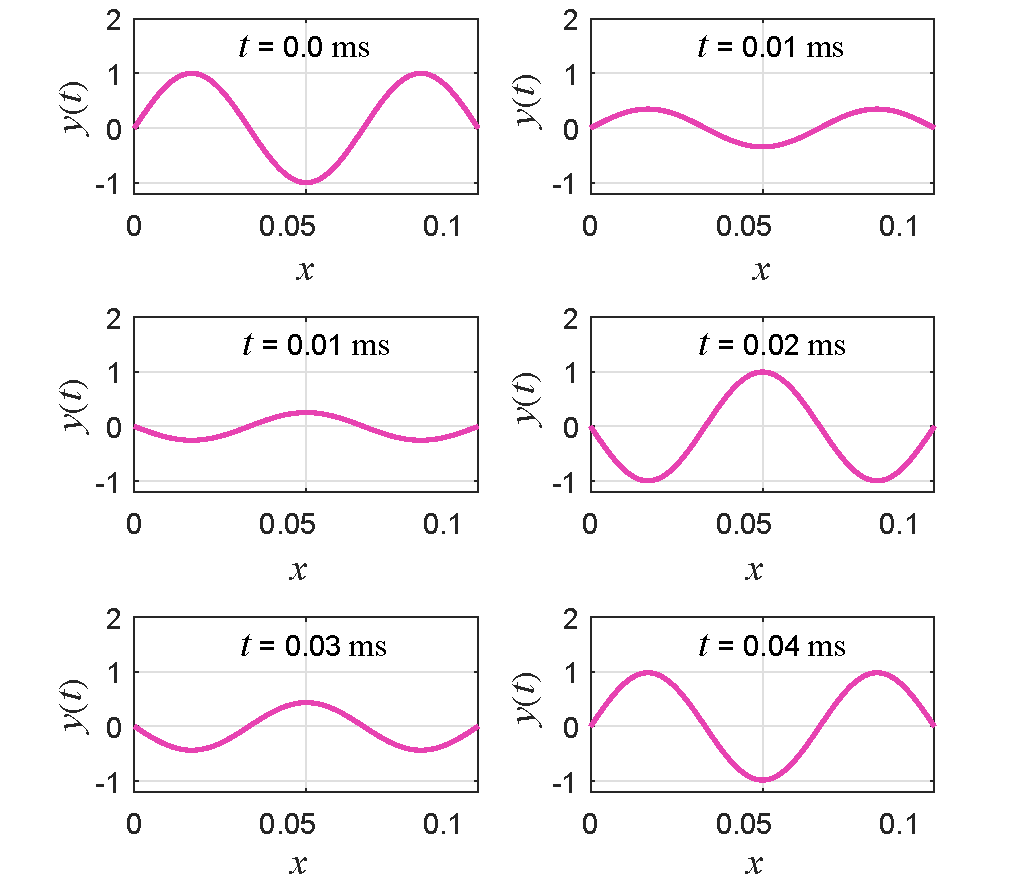
\includegraphics[width=\textwidth]{SchwingendeSaite01.pdf}
  \captionof{figure}{Stehende Welle\index{Welle!stehende} auf einer Saite. Siehe \mscr~ \mlkontmechref{SchwingendeSaite01.m}.}\label{abb:kontmech_SaiteStehendeWelle}
\end{center}

Selbstverst�ndlich k�nnen aber auch laufende Wellen\index{Welle!laufende}, f�r die analytische
L�sungen deutlich schwieriger zu finden sind mit dieser numerischen Methode
behandelt werden. Dies wollen wir in \probref{kontmech_WelleSaite}
tun.
\end{example}
% BEISPIEL %%%%%%%%%%%%%%%%%%%%%%%%%%%%%%%%%%%%%%%%%%%%%%%%%%%%%%%%%%%%%%%%%%%%%%%%%%%%%%%%%%

Geht man zu zwei Dimensionen �ber und betrachtet Schwingungen einer Ebene,
lassen sich die \emph{Chladnischen}\footnote{Ernst Florens Friedrich Chladni (1756--1827) war ein deutscher Physiker und Astronom. Er beschrieb die nach ihm benannten Klangfiguren und erkl�rte die Herkunft von Meteoriten.}\indexp{Chladni, Ernst Florens Friedrich} \emph{Klangfiguren} finden. Die zugeh�rige partielle
Differentialgleichung wird in \probref{kontmech_Chladni} gel�st.

Der gefundene kontinuierlichen Ansatz f�r die schwingende Saite l�sst sich
leicht erweitern. Ganz �hnlich l�sst sich z.B. das Problem der Achterbahn, die
in \probref{bew_achterbahn_diskret} durch diskrete Wagen simuliert wurde,
wieder aufgreifen, indem man den Grenzwert eines kontinierlichen Zuges bildet.
Auf diese Weise kann man sich dem kontinuierlichen Modell aus 
\kap{rollercoaster} ann�hern, ohne dabei die N�herung eines vollkommen
starren Zuges einf�hren zu m�ssen. Die Herleitung des Kontinuums-Grenzwerts
wird in \probref{kontmech_AchterbahnKont} durchgef�hrt,
\probref{kontmech_AchterbahnZug} widmet sich dann einer numerischen L�sung
und Betrachtungen f�r die Normalbeschleunigung erfolgen in
\probref{kontmech_AchterbahnBeschleunigungen}.


\subsubsection{Ausblick: Dynamik elastischer K�rper}
\label{kap:kontmech_festelastisch}
\index{K�rper!Dynamik elastischer}\index{K�rper!elastische}

Die Dynamik elastischer K�rper ist \iA sehr komplex. Dies hat
sich schon in \kap{kontmech_festEigenschaften} angedeutet,
da z.B. die Verl�ngerung eines K�rpers in der Regel auch eine Verk�rzung
in den Richtungen senkrecht dazu zur Folge hat. F�r eine vollst�ndige
Behandlung muss man alle Richtungen zusammen betrachten.
Ein solch umfangreicher Ansatz geht �ber den Umfang dieses Buches hinaus, wir verweisen auf die weiterf�hrende
Literatur, z.B. \cite{Altenbach1994,Altenbach2018,Rannacher2017}. Wir wollen hier aber angeben, welche Bewegungsgleichungen in der Dynamik elastischer K�rper gel�st werden m�ssen und
wie diese zu verstehen sind.

Als unabh�ngige Koordinaten f�r eine Ausgangskonfiguration bieten sich f�r
eine Betrachtung elastischer K�rper die materiellen Punkte $\vec{\hat{P}}$  nach der
Definition aus Gleichung \eqref{eq:kontmech_Materiepunkt} an. Wir w�hlen
jedoch die Materiepunkte nicht zu einem beliebigen Zeitpunkt $t_0$, sondern
so, dass sich alle Materiepunkte in einer Gleichgewichtslage befinden. In
dieser Gleichgewichtslage gilt also
\begin{equation*}
  \vec{r}_0 = \vec{\hat{P}}_0  \; .
\end{equation*}
Wir interessieren uns f�r die Auslenkungen eines Materiepunktes aus der Ruhelage, die wir mit $\vec{u}$ wollen:
\begin{equation*}
  \vec{u}(\vec{\hat{P}}) = \vec{r}(\vec{\vec{\hat{P}}}) - \vec{r}_{0}(\vec{\hat{P}})
  = \vec{r}(\vec{\hat{P}}) - \vec{\hat{P}}_0 \,.
\end{equation*}
Es ist zu erwarten, dass in einem
K�rper, der unter Spannung steht, diese Auslenkung f�r jeden Materiepunkt
verschieden ist\footnote{W�re sie f�r alle Punkte gleich, w�re dies nur
  eine Verschiebung des ganzen, unver�nderten K�rpers, was f�r die
  Betrachtung der inneren Dynamik uninteressant w�re.}. Alle m�glichen
Deformationen stellen wir durch die Ableitungen
\begin{equation}
  \frac{\partial r_i(\vec{\hat{P}})}{\partial r_j}
\end{equation}
dar. Sie enthalten Deformationen sowohl in L�ngs- als auch Querrichtung und
k�nnen prinzipiell als Elemente einer Matrix geschrieben werden.

Vollkommen analog betrachten wir die Spannungen im K�rper in allen m�glichen
Richtungen durch das Einf�hren des \emph{Spannungstensors}\index{Spannungstensor|textbf}
$\hat{\vec{\sigma}}$. Seine Diagonalelemente enthalten die Zug- und Druckspannungen,
w�hrend Scherspannungen in den Nichtdiagonalelementen notiert werden. Gehen wir
von einem Material aus, in dem die Deformationen linear von den Spannungen
abh�ngen, l�sst sich das verallgemeinerte Hooksche\indexp{Hooke, Robert}
Gesetz\index{Hooksches Gesetz}
\begin{equation}
    \hat{\vec{\sigma}} = \mathbb{C}\, \hat{\vec{\epsilon}} \quad \text{\bzw} \quad  \hat{\sigma}_{ij} = C_{ijkl} \,\hat{\epsilon}_{kl} 
\end{equation}
finden, wobei wir bei der Komponentenschreibweise die Einsteinschen Summenkonvention verwendet haben.
Im Spannungstensor $\hat{\vec{\sigma}}$ kommt der lineare und symmetrische
\emph{Verzerrungstensor}\index{Verzerrungstensor} $\hat{\vec{\epsilon}}$ vor:
\begin{align}
    \hat{\vec{\epsilon}} &= \frac{1}{2} \lk \nablav \vec{u} + \lk \nablav
    \vec{u} \rk^T \rk \quad \text{\bzw} \quad  \hat{\epsilon}_{kl} = \frac{1}{2} \lk \frac{\partial u_k}{\partial p_l} +
                 \frac{\partial u_l}{\partial p_k}  \rk \,.
\end{align}
Offensichtlich ist $\mathbb{C}$ ein Tensor vierter Stufe, der vier
Indizes besitzt. Ist das Material dar�ber hinaus isotrop, vereinfacht
sich der Zusammenhang und es ergeben sich die Beziehungen
\begin{subequations}
  \begin{align}
    \hat{\vec{\sigma}} &= 2 \mu \hat{\vec{\epsilon}} + \lambda \, \mathrm{Sp}(
                   \,\hat{\vec{\epsilon}}) \, \mathbb{I} \; , \\
    \hat{\vec{\sigma}} &= \mu \lk \nablav \vec{u} +  \lk \nablav \vec{u} \rk^T \rk
                   + \lambda \lk \nablav
                   \cdot \vec{u} \rk \,\mathbb{I}  \; , \\
    \hat{\sigma}_{ij} &= \mu \lk  \frac{\partial u_i}{\partial p_j} +
                  \frac{\partial u_j}{\partial p_i} \rk + \lambda
                  \,\frac{\partial u_k}{\partial p_k} \delta_{ij}
                  \label{eq:kontmech_Spannungstensor1}
  \end{align}
\end{subequations}
  mit der Einheitsmatrix $\mathbb{I}$. $\mathrm{Sp}(\hat{\vec{\epsilon}})$ ist die Spur des Tensors $\hat{\vec{\epsilon}}$ und die sogenannten \emph{Lam\'e}\footnote{Gabriel Lam\'e (1795--1870) war ein franz�sischer Mathematiker und Physiker, der 
auf dem Gebiet der Differentialgeometrie und der mathematischen Physik arbeitete. Er wurde ber�hmt f�r seine allgemeine L�sung der W�rmeleitungsgleichung.}\indexp{Lam\'e, Gabriel}-\emph{Konstanten}\index{Lam\'e-Konstanten} sind gegeben durch
\begin{subequations}
  \begin{align}
    \lambda &= \frac{\nu}{(1-2\nu)(1+\nu)} E \; ,\\
    \mu &= G = \frac{1}{2} \frac{1}{1+\nu} E \; ,
  \end{align}
\end{subequations}
wobei die zweite Lam\'e-Konstante $\mu$ dem bereits eingef�hrten Torsions-
oder \gls{Schubmodul}\index{Torsionsmodul}\index{Schubmodul} $G$ aus den
Gleichungen \eqref{eq:kontmech_Torsionsmodul1} bzw.
\eqref{eq:kontmech_Torsionsmodul3} entspricht und $\lambda$ offensichtlich in enger Beziehung zum Elastizit�tsmodul $E$ steht.

Dass die eingef�hrten Elastizit�ts- und Torsionsmodule aus den Kapiteln
\ref{kap:kontmech_festKontraktionen} und \ref{kap:kontmech_festtorsion}
die richtigen Spezialf�lle darstellen, die im dreidimensionalen
Spannungstensor enthalten sind, wird in \probref{kontmech_ElastizitaetTorsion}
herausgearbeitet. Als eine wichtige Anwendung von Spannungen in K�rpern wird
in \probref{kontmech_BogenSpannung} die Spannung eines Bogens durch eine
Saite untersucht.
  
Bleiben in der Dynamik alle Beziehungen linear, lautet die Bewegungsgleichung
f�r die Verzerrungen $\vec{u}$
  \begin{align}
    \varrho \,\frac{\partial^2 \vec{u}}{\partial t^2}
    &= \nabla \cdot \hat{\vec{\sigma}} + \varrho \,\vec{f} \quad \text{\bzw} \quad
    \varrho \,\frac{\partial^2 u_i}{\partial t^2}
    = \sum_j \frac{\partial \hat{\sigma}_{ji}}{\partial p_j} + \varrho\, f_i \; ,
  \end{align}
wobei $\vec{f}$ eine auf ein Volumenelement angreifende Kraftdichte in $\SI{}{\newton\per\metre\cubed}$ und
$\varrho$ die Massendichte ist.

\renewcommand\glslongextraNameAlign{p{36mm}}
\renewcommand\glslongextraDescAlign{p{60mm}}
\clearpage
\bgroup
\small
\printunsrtglossary[type=kontmech]
\egroup
\clearpage
\fancyhead[RE]{\nouppercase\rightmark}
\bibliography{referenzen}
\clearpage
\fancyhead[RE]{\nouppercase\leftmark}
%%%%%%%%%%%%%%%%%%%%%%%%%%%%%%%%%%%%%%%%%%%%%%%%%%%%%%%%%%%%
%\input{footer.tex}


%== pdf cut here end == %%%%%%%%

% Hier eigentliches pdf-Arbeitsbuch

\clearpage
\newpage
\fancyhf{}
\pagestyle{fancy}
\fancyhead[LE,RO]{\thepage}

%\documentclass[makeidx,envcountchap,graybox,deutsch,ngerman,sectrefs]{svmono}
%\documentclass[envcountchap,graybox,deutsch,sectrefs]{svmono}
%%%%% eigene tempor�re Abk�rzungsliste, f�r die Zeit, bis einheitliche Schreibungen bestehen
\usepackage{tempshort}
%%  Von Springer empfohlene Pakete %% 
%%\documentclass[envcountsect,graybox,deutsch,sectrefs]{svmono}
\usepackage{chapterbib}
\usepackage{type1cm}
\usepackage[ansinew]{inputenc}
\usepackage{babel}
\usepackage[pdftex]{graphicx} %PDF-Vektorgrafiken einbinden
\usepackage{newtxtext} %Typischer Springer-Font
\usepackage{newtxmath}
\usepackage{multicol}
\usepackage[bottom]{footmisc} %Platziert alle Fu�noten unten  
\usepackage[nobreak]{cite}
%\usepackage{biblatex}
\usepackage{cancel}
\usepackage[absolute]{textpos}
\usepackage{graphicx}
\usepackage{pdfpages}

%\usepackage{floatrow}
%\usepackage{mwe}
\usepackage[figuresright]{rotating}
\usepackage{bigints}
\let\laplace\relax  % Vermeidung der Fehlermeldung "\laplace already defined."
\usepackage{trfsigns}
\usepackage{amsmath}
\usepackage{tabulary}
\usepackage{tabularx}

%%  Eigene Pakete %%
\usepackage{adjustbox}
\usepackage{wasysym}
\usepackage{gensymb}
\usepackage{float}
\usepackage{caption}
\usepackage[left=5cm,right=4cm,top=3cm,bottom=4cm,includeheadfoot]{geometry}

%\usepackage{wasysym}
%\usepackage{bigints}
%\usepackage{esint}
%\usepackage{relsize,exscale}

\usepackage{mathtools}   % Vermeidung der Fehlermeldung "Undefined control sequence \coloneqq."


% header and footer
\usepackage{fancyhdr}
\pagestyle{fancy}
\fancyhead[LE,RO]\thepage
\renewcommand{\sectionmark}[1]{\markright{\thesection.\ #1}}
%\fancyhead[LO]{\nouppercase\leftmark}
%\fancyhead[RE]{\nouppercase\rightmark}
\fancyhead[LO]{\nouppercase\rightmark}
\fancyhead[RE]{\nouppercase\leftmark}
\fancyfoot{}
% svmono hat offenbar irgendwas merkw�rdig definiert, darum mu� hier verbreitert werden
%\addtolength\headwidth{25pt}
\setlength{\headheight}{25pt}

%% Units
\usepackage{siunitx}
\sisetup{
  locale = US,
  per-mode = reciprocal, %symbol, % | reciprocal | fraction | ?
  exponent-product = \cdot,
  separate-uncertainty,
  %exponent-to-prefix,
  %prefixes-as-symbols = false,
  %list-units = brackets,% | single | repeat
  %range-units = brackets,% | single | repeat
  %multi-part-units = brackets,% | single | repeat
}
\usepackage{chngcntr}
\usepackage{booktabs}
\usepackage{slashed}
\usepackage{listings}
\usepackage{color} %red, green, blue, yellow, cyan, magenta, black, white
%\usepackage{color} %Einfache Farbendefinition -> von Graybox-Option ben�tigt
\usepackage{multirow}
\usepackage{longtable} %Tabellen �ber mehrere Seiten hinweg
\usepackage{framed} % von Graybox-Option ben�tigt
\usepackage[shortlabels]{enumitem} %Erweiterte Aufz�hloptionen
\usepackage{array}
\usepackage[xindy]{imakeidx} %Wortindex und Personenindex erstellen

\usepackage[hyphens]{url}
%\usepackage[breaklinks,colorlinks=true,linkcolor=black,urlcolor=blue,citecolor=black,filecolor=green,hyperfootnotes=false]{hyperref}
\usepackage[                                    %Hyperref erstellt ein Bookmark/Lesezeichen im PDF. siehe https://www.namsu.de/Extra/pakete/Hyperref.html
bookmarksopen=true,															%Das Lesezeichen ist ge�ffnet beim �ffnen der PDF.
bookmarksnumbered=true,                         %Zahlen werden im Bookmark angezeigt.   
plainpages=false,
pdfpagelabels,
colorlinks=true,                                %Links werden farbig dargestellt.
linkcolor=black, citecolor=black, urlcolor=cyan %Farben definieren.
]{hyperref}                                     %Sollte als letztes eingebunden werden, da es sehr viele Verweise und �nderungen erzeugt. Das Packet ist sehr stark, aber auch umfangreich ist. 

%\usepackage[breaklinks,colorlinks=true,linkcolor=black,urlcolor=blue,citecolor=black,filecolor=green,hyperfootnotes=false]{hyperref}
%\usepackage[breaklinks,colorlinks=true,linkcolor=black,urlcolor=blue,citecolor=black,filecolor=green,hyperfootnotes=false
            %pdftex,
            %pdfauthor={Kaschke, Cartarius},
            %pdftitle={Finger�bungen der Physik}
            %pdfsubject={Ein Repetitorium und �bungsbuch zu im Studium wenig behandelten Kapiteln der Physik mit ausf�hrlich behandelten Problemen und MATLAB-Programmen},
            %pdfkeywords={Physik, Mechanik}
            %]{hyperref}
\pdfminorversion=5

\usepackage{hypcap}
\usepackage[record,section=section,stylemods={mcols},automake]{glossaries-extra}
\usepackage{glossary-longextra}
%\usepackage{glossary-bookindex}
%\makeindex
\setglossarystyle{long-name-sym-desc-loc}
\setabbreviationstyle[acronym]{long-short}

\definecolor{killA}{rgb}{.7,.3,.3}
\newcommand\killA[1]{\bgroup\color{killA}{\cancel{#1}}\egroup}
\newcommand\killB[1]{\bgroup\color{cyan!30!black}{\cancel{#1}}\egroup}

% typographisch korrekte Abk�rzungen (needs to be loaded after hyperref)
\usepackage{abbrev}
\newglossary*{bew}{Glossar}
\newglossary*{hm}{Glossar}
\newglossary*{adyn}{Glossar}
\newglossary*{kontmech}{Glossar}
\newglossary*{aero}{Glossar}
\newglossary*{edyn}{Glossar}
\newglossary*{spo}{Glossar}
\newglossary*{optbas}{Glossar}
\newglossary*{optger}{Glossar}
\newglossary*{optatm}{Glossar}
\newglossary*{optspez}{Glossar}
\GlsXtrLoadResources[src={bew/gloss},type=bew]
\GlsXtrLoadResources[src={hm/gloss},type=hm]
\GlsXtrLoadResources[src={adyn/gloss},type=adyn]
\GlsXtrLoadResources[src={kontmech/gloss},type=kontmech]
\GlsXtrLoadResources[src={aero/gloss},type=aero]
\GlsXtrLoadResources[src={spo/gloss},type=spo]
\GlsXtrLoadResources[src={edyn/gloss},type=edyn]
\GlsXtrLoadResources[src={optbas/gloss},type=optbas]
\GlsXtrLoadResources[src={optger/gloss},type=optger]
\GlsXtrLoadResources[src={optatm/gloss},type=optatm]
\GlsXtrLoadResources[src={optspez/gloss},type=optspez]
\glssetcategoryattribute{bew}{indexname}{true}
%\renewcommand\index\newterm
%\newcolumntype{g}[1]{>{\RaggedRight\hspace{0pt}}p{#1}}
%\renewcommand\glslongextraNameAlign{g}
\renewcommand\glslongextraLocationAlign{@{\ ~\ }>{\raggedright}p{\glspagelistwidth}}
\definecolor{gls}{rgb}{.4,.4,.5}
\renewcommand*{\glstextformat}[1]{\textcolor{gls}{#1}}

%Absatzregeln
\clubpenalty = 30000 %Keine einzelnen Absatzzeilen
\widowpenalty = 30000
\setlength{\parindent}{0em} 
\newcolumntype{L}[1]{>{\raggedright\arraybackslash}p{#1}}
\newcolumntype{C}[1]{>{\centering\arraybackslash}p{#1}}
\newcolumntype{R}[1]{>{\raggedleft\arraybackslash}p{#1}}

\usepackage{xstring}

\newcommand\mfile[2]{%
\saveexpandmode\noexpandarg
\StrSubstitute{#2}{_}{\_}[\tmpname]
\restoreexpandmode
\href{MatlabDateien/\chapname/#1\tmpname}{\tmpname}}

%%% Hyperlinks zu MATLAB Dateien
%\newcommand\mlref[1]{\mfile{}{#1}}
%\newcommand\mlinclref[1]{\mfile{IncludeFolder/}{#1}}
%\newcommand\mldataref[1]{\mfile{Data/}{#1}}

%%% .. f�r ein Verzeichnis hoch
%%% . f�r aktuelle Verzeichnis
%% lokal: MatlabDateien/bew
%\newcommand\mlbewref[1]{\href{MatlabDateien/bew/#1}{#1}}
%% git: https://github.com/sn-code-inside/fingeruebungen-physik/tree/main/bew

\newcommand{\mlrefwithindex}[2]{%
  \index[mfiles]{#2}%   <-- Eintrag im M-File-Index mit aktueller Seitenzahl
  \href{https://github.com/sn-code-inside/fingeruebungen-physik/tree/main/#1/#2}{#2}%
}


%\newcommand\mlbewref[1]{\href{https://github.com/sn-code-inside/fingeruebungen-physik/tree/main/bew/#1}{#1}}
%\newcommand\mlbewdref[1]{\href{https://github.com/sn-code-inside/fingeruebungen-physik/tree/main/bew/Data/#1}{#1}}
%\newcommand\mlbewiref[1]{\href{https://github.com/sn-code-inside/fingeruebungen-physik/tree/main/bew/IncludeFolder/#1}{#1}}
%\newcommand\mlkontmechref[1]{\href{https://github.com/sn-code-inside/fingeruebungen-physik/tree/main/kontmech/#1}{#1}}
%\newcommand\mlkontmechdref[1]{\href{https://github.com/sn-code-inside/fingeruebungen-physik/tree/main/kontmech/Data/#1}{#1}}
%\newcommand\mlkontmechiref[1]{\href{https://github.com/sn-code-inside/fingeruebungen-physik/tree/main/kontmech/IncludeFolder/#1}{#1}}
%\newcommand\mlhmref[1]{\href{https://github.com/sn-code-inside/fingeruebungen-physik/tree/main/hm/#1}{#1}}
%\newcommand\mlhmdref[1]{\href{https://github.com/sn-code-inside/fingeruebungen-physik/tree/main/hm/Data/#1}{#1}}
%\newcommand\mlhmiref[1]{\href{https://github.com/sn-code-inside/fingeruebungen-physik/tree/main/hm/IncludeFolder/#1}{#1}}
%\newcommand\mladynref[1]{\href{https://github.com/sn-code-inside/fingeruebungen-physik/tree/main/adyn/#1}{#1}}
%\newcommand\mladyndref[1]{\href{https://github.com/sn-code-inside/fingeruebungen-physik/tree/main/adyn/Data/#1}{#1}}
%\newcommand\mladyniref[1]{\href{https://github.com/sn-code-inside/fingeruebungen-physik/tree/main/adyn/IncludeFolder/#1}{#1}}
%\newcommand\mledynref[1]{\href{https://github.com/sn-code-inside/fingeruebungen-physik/tree/main/edyn/#1}{#1}}
%\newcommand\mledyndref[1]{\href{https://github.com/sn-code-inside/fingeruebungen-physik/tree/main/edyn/Data/#1}{#1}}
%\newcommand\mledyniref[1]{\href{https://github.com/sn-code-inside/fingeruebungen-physik/tree/main/edyn/IncludeFolder/#1}{#1}}
%\newcommand\mloptbasref[1]{\href{https://github.com/sn-code-inside/fingeruebungen-physik/tree/main/optbas/#1}{#1}}
%\newcommand\mloptbasdref[1]{\href{https://github.com/sn-code-inside/fingeruebungen-physik/tree/main/optbas/Data/#1}{#1}}
%\newcommand\mloptbasiref[1]{\href{https://github.com/sn-code-inside/fingeruebungen-physik/tree/main/optbas/IncludeFolder/#1}{#1}}
%\newcommand\mloptspezref[1]{\href{https://github.com/sn-code-inside/fingeruebungen-physik/tree/main/optspez/#1}{#1}}
%\newcommand\mloptspezdref[1]{\href{https://github.com/sn-code-inside/fingeruebungen-physik/tree/main/optspez/Data/#1}{#1}}
%\newcommand\mloptspeziref[1]{\href{https://github.com/sn-code-inside/fingeruebungen-physik/tree/main/optspez/IncludeFolder/#1}{#1}}

\newcommand\mlbewref[1]{\mlrefwithindex{bew}{#1}}
\newcommand\mlbewdref[1]{\mlrefwithindex{bew/Data}{#1}}
\newcommand\mlbewiref[1]{\mlrefwithindex{bew/Include}{#1}}
\newcommand\mlkontmechref[1]{\mlrefwithindex{kontmech}{#1}}
\newcommand\mlkontmechdref[1]{\mlrefwithindex{kontmech/Data}{#1}}
\newcommand\mlkontmechiref[1]{\mlrefwithindex{kontmech/Include}{#1}}
\newcommand\mlhmref[1]{\mlrefwithindex{hm}{#1}}
\newcommand\mlhmdref[1]{\mlrefwithindex{hm/Data}{#1}}
\newcommand\mlhmiref[1]{\mlrefwithindex{hm/Include}{#1}}
\newcommand\mladynref[1]{\mlrefwithindex{adyn}{#1}}
\newcommand\mladyndref[1]{\mlrefwithindex{adyn/Data}{#1}}
\newcommand\mladyniref[1]{\mlrefwithindex{adyn/Index}{#1}}
\newcommand\mledynref[1]{\mlrefwithindex{edyn}{#1}}
\newcommand\mledyndref[1]{\mlrefwithindex{edyn/Data}{#1}}
\newcommand\mledyniref[1]{\mlrefwithindex{edyn/Index}{#1}}
\newcommand\mloptbasref[1]{\mlrefwithindex{optbas}{#1}}
\newcommand\mloptbasdref[1]{\mlrefwithindex{optbas/Data}{#1}}
\newcommand\mloptbasiref[1]{\mlrefwithindex{optbas/Include}{#1}}
\newcommand\mloptspezref[1]{\mlrefwithindex{optspez}{#1}}
\newcommand\mloptspezdref[1]{\mlrefwithindex{optspez/Data}{#1}}
\newcommand\mloptspeziref[1]{\mlrefwithindex{optspez/Include}{#1}}
\newcommand\mloptgerref[1]{\mlrefwithindex{optger}{#1}}
\newcommand\mloptgerdref[1]{\mlrefwithindex{optger/Data}{#1}}
\newcommand\mloptgeriref[1]{\mlrefwithindex{optger/Include}{#1}}
\newcommand\mloptatmref[1]{\mlrefwithindex{optatm}{#1}}
\newcommand\mloptatmdref[1]{\mlrefwithindex{optatm/Data}{#1}}
\newcommand\mloptatmiref[1]{\mlrefwithindex{optatm/Include}{#1}}



\newcommand\mlcmd[1]{\textcolor{cyan}{\texttt{#1}}}

%Grafikregeln
\graphicspath{{hm/graphs/}
	                    	{bew/graphs/}
     						{kontmech/graphs/}
							{hm/graphs/}
							{adyn/graphs/}
							{edyn/graphs/}
							{kontmech/graphs/}
							{spo/graphs/}
							{optbas/graphs/}
							{optger/graphs/}
							{optatm/graphs/}
							{solman/graphs/}
                                                        {aero/graphs}}
\DeclareGraphicsExtensions{.pdf, .png, .jpg, .jpeg}
\def\figname{Abb}
\newcommand\figref[1]{\figname.\ \ref{abb:#1}}
\usepackage[labelfont=bf]{caption}

\usepackage{tocloft}
\usepackage{etoc}
\setlength\cftfignumwidth{30pt}

% Flatterrand links
\cftsetindents{chapter}{0em}{4em}
\cftsetindents{section}{1.5em}{4em}
\cftsetindents{subsection}{3.8em}{4em}

% flacher Rand links
%\cftsetindents{chapter}{0em}{4em}
%\cftsetindents{section}{0em}{4em}
%\cftsetindents{subsection}{0em}{4em}

\newcommand\partitle[1]{
\addcontentsline{toc}{part}{#1}
\begin{titlepage}
  %\vskip 60%\p@
  \begin{center}
    {\LARGE Finger�bungen der Physik -- #1 \par}
    \vskip 3em%
    {\large Michael Kaschke und Holger Cartarius\par}
  \end{center}
\end{titlepage}
}

%\newcommand\mlref[1]{\href{\chapname/matlab/#1}{#1}}
%\newcommand\mlinclref[1]{\href{\chapname/matlab/IncludeFolder/#1}{\color{cyan}{#1}}}

%Neue Kommandos
\newcommand{\lk}{\left(}        %gro�e runde Klammer (links)
\newcommand{\rk}{\right )}      %gro�e runde Klammer (rechts)
\newcommand{\lgk}{\left \{}     %gro�e geschweifte Klammer (links)
\newcommand{\rgk}{\right \}}    %gro�e geschweifte Klammer (rechts)
\newcommand{\lek}{\left [}      %gro�e eckige Klammer (links)
\newcommand{\rek}{\right ]}     %gro�e eckige Klammer (rechts)
\newcommand{\anf}[1]{\glqq#1\grqq}    %Deutsche Anf�hrungszeichen: \anf{}
\newcommand{\defined}{:=}				%Definition
\newcommand{\curl}{\text{\textbf{rot}}\,}	%Rotation-Operator curl()
\newcommand{\ket}[1]{|#1\rangle}		%Quantenmechanischer Zustand
\newcommand{\curvelintri}{\,\overset{\blacktriangle}{\smallfrown}}
\newcommand{\straighttri}{\blacktriangle}
\newcommand{\UT}{\text{UT}}
\newcommand{\UTC}{\text{UTC}}
\newcommand{\JD}{\text{JD}}
\newcommand{\JDE}{\text{JDE}}
\newcommand{\MJD}{\text{MJD}}
\newcommand{\TDT}{\text{TDT}}
\newcommand{\TT}{\text{TT}}
\newcommand{\NVS}{\text{Navier-Stokes-Gleichungen}}
\newcommand{\MWG}{\text{Maxwell-Gleichungen}}
\newcommand{\EMW}{\text{Elektromagnetische Wellen}}
\newcommand{\eMW}{\text{elektromagnetischen Wellen}}
\newcommand{\RT}{\text{Relativit�tstheorie~}}
\newcommand{\au}{\mathrm{AE}}
\newcommand{\ET}{\text{ET}}
\newcommand{\TAI}{\text{TAI}}
\newcommand{\GMST}{\text{GMST}}
\newcommand{\LMST}{\text{LMST}}
\newcommand{\MESZ}{\text{MESZ}}
\newcommand{\KOS}{\text{Koordinatensystem }}
\newcommand{\DGL}{\text{Differentialgleichung }}
\newcommand{\NA}{\text{NA}}
\newcommand{\uA}{\text{u}}  %atomare Masseneinheit
\newcommand{\MOZ}{\text{MOZ}}
\newcommand{\grad}{\text{\textbf{grad}}\,}	%Gradient-Operator grad()
\newcommand{\uproman}[1]{\mathrm{\uppercase\expandafter{\romannumeral#1}}}
\newcommand{\lowroman}[1]{\romannumeral#1\relax}

\newcommand\todo[1]{\textcolor{red}{TODO: #1}}

\renewcommand{\=}[1]{\stackrel{\text{#1}}{=}}  %Schrift �ber Gleich-Zeichen
\renewcommand{\d}{\partial}
\newcommand{\lra}{\Leftrightarrow}  %�quivalenz-Pfeile
\newcommand{\abs}[1]{\left\vert#1\right\vert}     %Betragsklammern
\renewcommand{\Re}{\mathrm{Re}}                          %Realteil
\renewcommand{\Im}{\mathrm{Im}}                          %Imagin�rteil
\renewcommand{\im}{\mathrm{i}}                         %Imagin�re Einheit
\renewcommand{\epsilon}{\varepsilon} 
\newcommand{\keff}{k_\text{eff}}
\newcommand{\con}{\text{const}}
\newcommand{\conv}{\vec{const}}
\newcommand{\PL}{\mathcal{P}_}
\newcommand{\artanh}{\mathrm{artanh}}
% QED-Symbol im text- bzw. Mathemodus
\newcommand{\textqed}{\hfill ~ $\square$}
\newcommand{\mmqed}{\tag*{$\square$}}

\newcommand{\fa}{(\textbf{a}) }
\newcommand{\fb}{(\textbf{b}) }
\newcommand{\fc}{(\textbf{c}) }
\newcommand{\fd}{(\textbf{d}) }
\newcommand{\fe}{(\textbf{e}) }
\newcommand{\ff}{(\textbf{f}) }

\newcommand{\iF}{im Folgenden~}
\newcommand{\iA}{im Allgemeinen~}


\DeclareMathOperator\divv{div}
\DeclareMathOperator\res{Res}
\DeclareMathOperator{\sech}{sech}
\DeclareMathOperator\sgn{sgn}

% f�r Appendix - MATLAB Referenz
\newcommand{\rotv}{\vec{rot}\,}
\newcommand{\gradv}{\vec{grad}\,}
\newcommand{\nablav}{\vec{\nabla}\,}

\newcommand{\ceil}{\mathrm{ceil}}
\newcommand{\sinc}{\mathrm{sinc}}
\newcommand{\diag}{\mathrm{diag}}
\newcommand{\sign}{\mathrm{sign}}
\newcommand{\length}{\mathrm{length}}
\newcommand{\sort}{\mathrm{sort}}
\newcommand{\summ}{\mathrm{sum}}
\newcommand{\asin}{\mathrm{asin}}
\newcommand{\acos}{\mathrm{acos}}
\newcommand{\atan}{\mathrm{atan}}
\newcommand{\prodd}{\mathrm{prod}}
\newcommand{\median}{\mathrm{mediab}}
\newcommand{\mean}{\mathrm{mean}}
\newcommand{\std}{\mathrm{std}}
\newcommand{\eye}{\mathrm{eye}}
\newcommand{\zeros}{\mathrm{zeros}}
\newcommand{\ones}{\mathrm{ones}}
\newcommand{\rand}{\mathrm{rand}}
\newcommand{\inline}{\mathrm{inline}}
\newcommand{\modd}{\mathrm{mod}}
\newcommand{\floor}{\mathrm{floor}}
\newcommand{\round}{\mathrm{round}}
\newcommand{\rem}{\mathrm{rem}}
\newcommand{\sqrtt}{\mathrm{sqrt}}
\newcommand{\triu}{\mathrm{triu}}
\newcommand{\tril}{\mathrm{tril}}
\newcommand{\size}{\mathrm{size}}
\newcommand{\dett}{\mathrm{det}}
\newcommand{\inv}{\mathrm{inv}}
\newcommand{\rank}{\mathrm{rank}}
\newcommand{\rref}{\mathrm{rref}}
\newcommand{\eig}{\mathrm{eig}}
\newcommand{\poly}{\mathrm{poly}}
\newcommand{\lu}{\mathrm{lu}}
\newcommand{\qr}{\mathrm{qr}}
\newcommand{\quaddd}{\mathrm{quad}}
\newcommand{\fzero}{\mathrm{fzero}}
\newcommand{\roots}{\mathrm{roots}}
\newcommand{\odezd}{\textcolor{mygreen}{\texttt{ode23}}}
\newcommand{\odevf}{\textcolor{mygreen}{\texttt{ode45}}}
\newcommand{\odeeds}{\textcolor{mygreen}{\texttt{ode13s}}}
\newcommand{\odeefs}{\textcolor{mygreen}{\texttt{ode15s}}}
\newcommand{\ddezd}{\textcolor{mygreen}{\texttt{dde23}}}
\newcommand{\onlineZ}{online verf�gbaren Zusatzmaterialien{}}
\newcommand{\MKc}{\url{https://www.fingeruebungen-physik.de}{}}
\newcommand{\linklsg}{\href{https://www.fingeruebungen-physik.de}{\textcolor{blue} {$\rightarrow$ L�sungsteil.}}}
\newcommand{\githubSN}{\url{https://github.com/sn-code-inside/fingeruebungen-physik}{}\,\,}

\newcommand{\FT}{\mathcal{F}} %Fourier-Transformierte

% Aufz�hlung der L�sungen der Teilaufgaben
\newlist{subprobs}{enumerate}{1}
\setlist[subprobs]{
  label= \textbf{\textit{Teilaufgabe}} \textbf{\textit{\arabic*:}} \protect\thissubprob,
  ref=\arabic*, itemsep=\baselineskip, align=left}
\newcommand{\subprob}[1]{
  \def\thissubprob{\textbf{\textit{#1}}}\item ~\vspace{0.2\baselineskip} \newline}

\renewenvironment{example}[1]{
\refstepcounter{example}\par\medskip
\begin{shaded} 
\begin{samepage}
\noindent \textbf{\textit{Beispiel~\theexample: {#1}}}\\ 
\noindent{\color{black} \rule{\textwidth}{0.2 mm}}
\end{samepage}
}{\end{shaded}
\noindent{\color{black} \rule{\textwidth}{0.2 mm}}
} % or snugshade
\definecolor{shadecolor}{gray}{0.95}
\definecolor{mygreen}{RGB}{28,172,0} % color values Red, Green, Blue
\definecolor{mylilas}{RGB}{170,55,241}

\newenvironment{infobox}[1]{
     \begin{shaded} 
     \begin{samepage}
\noindent{\color{black} \rule{\textwidth}{0.2 mm}}
     \end{samepage}
}{\end{shaded}
\noindent{\color{black} \rule{\textwidth}{0.2 mm}}
} 
\definecolor{shadecolor}{gray}{0.95}
\definecolor{mygreen}{RGB}{28,172,0} % color values Red, Green, Blue
\definecolor{mylilas}{RGB}{170,55,241}


\newenvironment{nebenrechnung}[1]{
\begin{shaded} 
\begin{samepage}
\noindent\textbf{Nebenrechnung: \\} 
\noindent{\color{black} \rule{0.1\columnwidth}{0.2mm} \\}
\end{samepage}
}{\end{shaded}
\noindent{\color{black} \rule{0.1\columnwidth}{0.2mm} \\}
} % or snugshade
\definecolor{shadecolor}{gray}{0.95}
\definecolor{mygreen}{RGB}{28,172,0} % color values Red, Green, Blue
\definecolor{mylilas}{RGB}{170,55,241}

\newenvironment{merksatz}[1]{
\begin{shaded} 
\begin{samepage}
\noindent\textbf{Merke:\\} 
\noindent{\color{black} \rule{0.9\columnwidth}{0.2mm} \\ \\}
\end{samepage}
}{\end{shaded}
\noindent{\color{black} \rule{0.9\columnwidth}{0.2mm} \\}
} % or snugshade


\lstset{language=Matlab,%
    %basicstyle=\color{red},
    %basicstyle={\linespread{0.9}\ttfamily},
    basicstyle=\footnotesize\ttfamily,
    breaklines=true,%
    morekeywords={matlab2tikz},
    keywordstyle={\small \color{mygreen}},%
    morekeywords=[2]{1}, keywordstyle=[2]{\small\color{black}},
    identifierstyle={\small \color{black}},%
    stringstyle={\small\color{mylilas}},
    commentstyle={\small\color{mylilas}},%
    showstringspaces=false,%without this there will be a symbol in the places where there is a space
    numbers=left,%
    numberstyle={\tiny \color{black}},% size of the numbers
    numbersep=9pt, % this defines how far the numbers are from the text
    emph=[1]{for,end,else,break, function},emphstyle=[1]\small \color{blue}, %some words to emphasise
    emph=[2]{odeset},emphstyle=[2]\small \color{mygreen}, %some words to emphasise
    %emph=[2]{word1,word2}, emphstyle=[2]{style},    
}

%\bibliographystyle{spphys.bst}

%Trennregeln f�r spezielle Worte
%\hyphenation{Fresnel \matlab �qui-nok-ti-um}

\DeclareSIUnit\erg{erg}
\DeclareSIUnit\cal{cal}
\DeclareSIUnit\celsius{C}
\DeclareSIUnit\m{M}
\DeclareSIUnit\kel{K^{-4}}

%Stichwort- und Personenverzeichnis
\makeindex[title=Stichwortverzeichnis] % Create the default index
\makeindex[name=personen,title=Personenverzeichnis] % Create an index named 'personen'
\newcommand{\indexp}[1]{\index[personen]{#1}}
\makeindex[name=mfiles,title=MATLAB-Skriptverzeichnis,columns=2]

% list of exercises
\newcommand{\loxname}{\Large �bungsverzeichnis}  % einheitliche Gr��e Large
\newlistof[chapter]{prob}{lox}\loxname
\newcommand\uebung[3][]{\label{prob:#2}%
\addcontentsline{lox}{prob}{\protect\numberline{}{\probRef{#2}:~#3#1}}%
\textbf{#1#3}\\[\baselineskip]}
\makeatletter
\renewcommand{\l@prob}{\@dottedtocline{1}{0em}{0em}}
\makeatother

\newcommand\einfach{\uebung[~$\ast$~~]}
\newcommand\mittel{\uebung[~$\ast\,\ast$~~]}
\newcommand\schwierig{\uebung[~$\ast\,\ast\,\ast$~~]}
\newcommand\zusatz{\uebung[~$\ast\,\ast\,\ast\,!$~~]}
%\newcommand\einfach{\uebung[~\textbf{*}~~]}
%\newcommand\mittel{\uebung[~\textbf{*\,*}~~]}
%\newcommand\schwierig{\uebung[~\textbf{*\,*\,*}~]}
%\newcommand\zusatz{\uebung[~\textbf{*\,*\,*\,!}~~]}
\usepackage[atend]{bookmark}
%\BookmarkAtEnd{%
%\bookmarksetup{startatroot}\bookmark[level=0,named=\loxname]{}}

\newcommand\kapitel[1]{Kapitel \ref{kap:#1}}
%\newcommand\kap[1]{Kap.\ \ref{kap:#1}}
\newcommand\kap[1]{Kap. \ref{kap:#1}}

\begin{document}
% customize prob and sol in svmono
\makeatletter
%\counterwithin*{chapter}{part}

\spn@wtheorem{prob}{\bgroup\exercisename\egroup}{\bfseries}{\rmfamily}
\makeatother
\renewenvironment{sol}[1]{\par\addvspace{6pt}\noindent\phantomsection{\textbf{L�sung \ref{#1}}} \ignorespaces}{\par\addvspace{6pt}}
\newcommand\probRef[1]{�bung \ref{prob:#1}}
\renewcommand\probref[1]{\textbf{\probRef{#1}}}
\newcommand\lsgref[1]{L�sung \ref{lsg:#1}}

\newcommand\sbullet[1][.5]{\mathbin{\vcenter{\hbox{\scalebox{#1}{$\bullet$}}}}}

\setcounter{table}{0}



% f�r funktionierende Hyperlinks zwei neue Environments mit eigenen Countern, up. 2024-01-29

% f�r funktionierende Hyperlinks zwei neue Environments mit eigenen Countern, up. 2024-01-29
\newcounter{partsectionU}
\newcounter{partsectionL}
\newcounter{partsectionA}

\newenvironment{PartU}[1]
 {%
  \cleardoublepage
  \phantomsection
  \setcounter{section}{\value{partsectionU}}%
  \renewcommand{\thesection}{\"U\arabic{section}}%
  \renewcommand{\theHsection}{SU\arabic{section}}%
  \addcontentsline{toc}{part}{#1}%
  \thispagestyle{empty}
  \begin{flushright}
    \LARGE
    \textbf{ �bungen -  Band I  Mechanik\\}
  \end{flushright}
  \vspace*{\fill}
  \clearpage
 }
 {
  \setcounter{partsectionU}{\value{section}}%
  \cleardoublepage
}

\newenvironment{PartL}[1]
 {%
  \cleardoublepage
  \phantomsection
  \setcounter{section}{\value{partsectionL}}%
  \renewcommand{\thesection}{L\arabic{section}}%
  \renewcommand{\theHsection}{SL\arabic{section}}%
  \addcontentsline{toc}{part}{#1}%
  \thispagestyle{empty}
  \begin{flushright}
    \LARGE
    \textbf{L�sungsvorschl�ge - Band I Mechanik\\}
  \end{flushright}
  \vspace*{\fill}
  \clearpage
 }
 {
  \setcounter{partsectionL}{\value{section}}%
 \cleardoublepage
}

\newenvironment{PartA}[1]
 {%
  \cleardoublepage
  \phantomsection
  \setcounter{section}{\value{partsectionA}}%
  \renewcommand{\thesection}{A\arabic{section}}%
  \renewcommand{\theHsection}{SA\arabic{section}}%
  \addcontentsline{toc}{part}{#1}%
  \thispagestyle{empty}
  \begin{flushright}
    \LARGE
    \textbf{Appendix - Band I Mechanik\\}
  \end{flushright}
  \vspace*{\fill}
  \clearpage
 }
 {%
  \setcounter{partsectionA}{\value{section}}%
 \cleardoublepage
}

%%%%%%%%%%%%%%%%%%%%%%%%%%%%%%%%%%%%%%%%%%%%%%%%%%%%%%%%%%%%%

\bibliographystyle{spphys}

\makeatletter
\@addtoreset{chapter}{part}
\makeatother
\renewcommand{\thechapter}{�\,\arabic{chapter}}
\setcounter{page}{0}

\addtocontents{toc}{\protect\setcounter{tocdepth}{2}}% alles zeigen

\begin{PartU}{�bungen - Band I  Mechanik}
\setcounter{chapter}{1}
\setcounter{section}{0}
\setcounter{subsection}{0}
\setcounter{figure}{0}
\setcounter{equation}{0}
\setcounter{prob}{0}
\counterwithin{table}{section}
\setcounter{table}{0}
\newpage
\quad 
\thispagestyle{empty}
\newpage
\input{bew/bew_uebungenAB}
\newpage 
\thispagestyle{empty}
\quad 
\newpage
\setcounter{chapter}{2}
\setcounter{figure}{0}
\setcounter{equation}{0}
\setcounter{prob}{0}
\counterwithin{table}{section}
\setcounter{table}{0}
%%% Anmerkung 2024-01-14 (hc.):
%%% Kommentierungen f�r AB gesetzt (vgl. dazu Kommentar von mk in
%%% kontmech_uebenen.tex):
%%% 
%%% Links auf L�sungen hier gesetzt, da extra file kontmech_uebungenAB.tex
%%% Einfaches �ndern durch  ersetzen %\hyperref.. <--> \hyperref.
%%% Links auf L�sungsbank auskommentiert.
%%% Einfaches �ndern durch  ersetzen %%\href{FingerUeb1_AB.pdf.. <--> %\href{FingerUeb1_AB.pdf..


\section{�bungen zu Kapitel \ref{chap:kontmech} -- Physik des Kontinuums}\label{kap:kontmech_uebungen}

\medskip
Die �bungen sind mit Schwierigkeitsindikatoren markiert, von einfach ($\ast$) �ber mittel ($\ast \ast$) bis schwierig ($\ast \ast \ast$).
Zusatzaufgaben sind zum Teil mit ($\ast \ast \ast \;!$) markiert und eher als Erweiterung des Theorieteils zu betrachten.
Einige wenige �bungen sind rein analytisch, die gro�e Mehrzahl beinhaltet aber \matlab-Anwendungen. 
Die entsprechenden \mscre finden sich im GitHub unter \githubSN \, \bzw
in den \onlineZ{} (\MKc).\\

%-----------------------------------------------------------------------------------------------------------

\subsection{�bungen zu Bewegungen von Fl�ssigkeiten und Gasen}

\medskip

%-----------------------------------------------------------------------------------------------------------

\begin{prob} %�bung1
\einfach{kontmech_diffoperators}{Differentialoperatoren}
Berechnen Sie numerisch die Differentialoperatoren der folgenden Felder und stellen Sie die Felder und die Differentialoperatoren graphisch jeweils passend als Kontur- und 3D-Graphik dar.
\begin{enumerate}
	\item $\gradv \varphi$ f�r
\begin{subequations}
		\begin{align}
			\varphi(\vec{r}) &= (x\,y)\,\e^{-r^2}\,,\quad r^2 = x^2+y^2+z^2\,, \label{eq:kontmech_uebg1_1a}  \\
			\varphi(\vec{r}) &=  C\,\frac{\e^{-\alpha\,r}}{r}\,,\quad r^2 = x^2+y^2+z^2~~~~\text{(Yukawa-Potential)}\,.\indexp{Yukawa, Hideki} \label{eq:kontmech_uebg1_1b}
		\end{align}
\end{subequations}
	\item $\divv \vec{f}$ f�r 
		\begin{align}
			\vec{f}(\vec{r}) &= \begin{pmatrix} x-z\\xz\\y^2\end{pmatrix} \quad \text{und} \quad 
			\vec{f}(\vec{r}) = \begin{pmatrix} 5x^2\\3y^2\\0\end{pmatrix} \,. \label{eq:kontmech_uebg1_2}
		\end{align}
	\item $\rotv \vec{f}$ f�r 
		\begin{align}
			\vec{f}(\vec{r}) &= 0.5\, \begin{pmatrix} yz^2\\-xz^2\\0\end{pmatrix} \quad \text{und} \quad 
			\vec{f}(\vec{r}) = \begin{pmatrix} 0\\2xz+3y^2\\4yz^2\end{pmatrix} \,. \label{eq:kontmech_uebg1_3}
		\end{align}
\end{enumerate}

\medskip
\hyperref[lsg:kontmech_diffoperators]{\textcolor{blue} {$\rightarrow$ L�sungsvorschlag}}.\\
%\href{FingerUeb1_AB.pdf#lsg:kontmech_diffoperators}{\textcolor{blue} {$\rightarrow$ L�sungsteil}}.\\

\noindent\rule[1ex]{\textwidth}{0.5pt}
\end{prob}

%-----------------------------------------------------------------------------------------------------------
\begin{prob} %�bung2
  \einfach{kontmech_ueb_vectoranalysis}{�bungen zur Vektorrechnung und Vektoranalysis}

Folgende �bungen werden zur Festigung der Fertigkeiten in der Vektorrechnung und Vektoranalysis empfohlen:
\begin{itemize}
  \item Beweisen Sie die Gra�mann\footnote{Hermann G�nther Gra�mann (1809 -- 1877) war ein deutscher Mathematiker und Physiker. Er gilt als einer der Begr�nder der Vektor- und Tensorrechnung.}\indexp{Gra�mann, Hermann G�nther}\index{Gra�mann-Identit�t}-Identit�t (\ref{eq:kontmech_vecbasics04}\,b) in kartesischen Koordinaten. Wiederholen Sie die Rechnung unter jeweiliger Verwendung des Levi-Civita-Symbols \eqref{eq:kontmech_levicivita} und der Einsteinschen Summenkonvention (Gl. \eqref{eq:kontmech_dot_cross_einstein}).
  \item Wiederholen Sie \probref{bew_KOS_Formel}, diesmal jedoch unter Verwendung der Jacobi-Matrix\index{Jacobi-Matrix}:
	\begin{equation}
   \mathbb{J} = \begin{pmatrix} \frac{\d x}{\d x'} & \frac{\d x}{\d y'} & \frac{\d x}{\d z'} \\
                               \frac{\d y}{\d x'} & \frac{\d y}{\d y'} & \frac{\d y}{\d z'} \\
                               \frac{\d z}{\d x'} & \frac{\d z}{\d y'} & \frac{\d z}{\d z'} \end{pmatrix} \quad \text{\bzw} \quad J_{i,j} = \frac{\d x_i}{d x_j{}'} \,. \label{eq:kontmech_jacobimatrix}
	\end{equation}
	Hierin sind $x,y,z$ die kartesischen Koordinaten und $x', y', z'$ die Kugel- \bzw Zylinderkoordinaten, also $r, \phi, \theta$ \bzw $\rho, \phi, z$ 
  \item Berechnen Sie nun, wiederum unter Verwendung der Jacobi-Matrix, $\gradv \varphi$, $\divv \vec{f}$, $\rotv \vec{f}$ und $\gradv \vec{f}$ in Zylinder- und Kugelkoordinaten.
\end{itemize}
  
  \medskip  
	
	\medskip
\hyperref[lsg:kontmech_ueb_vectoranalysis]{\textcolor{blue} {$\rightarrow$ L�sungsvorschlag}}.\\
%\href{FingerUeb1_AB.pdf#lsg:kontmech_ueb_vectoranalysis}{\textcolor{blue} {$\rightarrow$ L�sungsteil}}.\\

\noindent\rule[1ex]{\textwidth}{0.5pt}
\end{prob}

%-----------------------------------------------------------------------------------------------------------
\begin{prob} %�bung3
\mittel{kontmech_integralsaetze}{Integrals�tze der Vektoranalysis}
�berpr�fen \bzw berechnen Sie jeweils analytisch und numerisch:
\begin{enumerate}
	\item den Integralsatz von Stokes f�r die Vektorfelder nach \eqref{eq:kontmech_uebg1_3} f�r einen Einheitskubus ohne Deckel ($z=1$).
	\item den Integralsatz von Stokes f�r die Vektorfelder nach \eqref{eq:kontmech_uebg1_3} f�r ein Einheitsquadrat bei $z=1$ parallel zur $x$-$y$-Ebene und eines bei $y=1$ parallel zur $x$-$z$-Ebene.
	\item den Integralsatz von Gau� f�r die Vektorfelder nach \eqref{eq:kontmech_uebg1_2} f�r einen Einheitskubus mit Zentrum im Ursprung, der entlang der kartesischen Achsen ausgerichtet ist.
	\item unter Benutzung des Integralsatzes von Gau� das Volumen eines Fasses der H�he $h$, wobei 
	\begin{enumerate}[i)]
	\item das Fass einen $z$-abh�ngigen Radius in $z \in [0,h]$ mit $r(z) = r_0\,\sqrt{1+C\, \sin(\pi\,z/h)}$ habe \bzw 
	\item das Fass die Form einer um die $z$-Achse rotierenden Ellipse habe, f�r die $x^2/3^2 + z^2/2^2 = 1 (z \in [-h,h])$ gilt. 
  \end{enumerate}
   Berechnen Sie das Volumen des Fasses mit der H�he $h=\SI{2}{\metre}$ und einem Deckfl�chenradius-Radius von $R=\SI{1}{\metre}$ und einer Mittendicke von $a=\SI{1.5}{\metre}$ .
\end{enumerate}

\medskip
\hyperref[lsg:kontmech_integralsaetze]{\textcolor{blue} {$\rightarrow$ L�sungsvorschlag}}.\\
%\href{FingerUeb1_AB.pdf#lsg:kontmech_integralsaetze}{\textcolor{blue} {$\rightarrow$ L�sungsteil}}.\\

\noindent\rule[1ex]{\textwidth}{0.5pt}
\end{prob}


%-----------------------------------------------------------------------------------------------------------

\begin{prob} %�bung4
\einfach{kontmech_bernoulli}{Bernoulli-Gleichung}
Leiten Sie die Bernoulli-Gleichung direkt aus der Euler-Gleichung her.\\

\medskip
\hyperref[lsg:kontmech_bernoulli]{\textcolor{blue} {$\rightarrow$ L�sungsvorschlag}}.\\
%\href{FingerUeb1_AB.pdf#lsg:kontmech_bernoulli}{\textcolor{blue} {$\rightarrow$ L�sungsteil}}.\\

\noindent\rule[1ex]{\textwidth}{0.5pt}
\end{prob}

%-----------------------------------------------------------------------------------------------------------
\begin{prob} %�bung5
\mittel{kontmech_magnus}{Magnus-Effekt, Flettner-Rotoren}
Bereits in den 20er Jahren des 20. Jahrhunderts entwickelte Anton Flettner\footnote{Anton Flettner (1885--1961) war ein Ingenieur und Erfinder, der �ber 1000 Patente anmeldete, vor allem f�r technische L�sungen in der Schifffahrt und der Flugzeugtechnik.}\indexp{Flettner, Anton} Wind\-antriebssysteme f�r Schiffe, die den \emph{Magnus}\indexp{Magnus, Heinrich Gustav }\footnote{Heinrich Gustav Magnus (1802--1870) war ein deutscher Physiker und Chemiker, der als Professor an der Humboldt-Universit�t zu Berlin als Begr�nder einer der wichtigsten Physikerschulen des 19. Jahrhunderts gilt. Zu seinen Sch�lern z�hlten \ua  Hermann von Helmholtz\indexp{Helmholtz, Hermann von}.}\emph{-Effekt} nutzbar machten. Der Magnus-Effekt besagt, dass ein rotierender, runder K�rper (Zylinder oder Kugel), der von einem Fluid umstr�mt wird, eine Querkraft erf�hrt.\footnote{Man m�chte Albert Einstein\indexp{Einstein, Albert} nur zustimmen, der zu den Flettner-Rotoren schrieb, "`dass die Wirkungsweise der Flettner-Rotoren dem Laien meist ein Mysterium bleibt, trotzdem dabei nur rein mechanische Wirkungen zur Verwendung kommen, die jeder gef�hlsm��ig zu beherrschen glaubt"'.} Obwohl die von Flettner auf dieser Idee  konstruierten Schiffe erfolgreiche Probefahrten absolvierten, konnte sich das Rotorsystem aus rein wirtschaftlichen Gr�nden nicht durchsetzen. Heute ist das System wegen der erzielbaren Energieeinsparung und der Reduktion der Kohlendioxid-Emission durch die Schifffahrt wieder h�ufiger auf den Weltmeeren zu sehen, \ua bei den Ostseef�hren zwischen Deutschland und D�nemark (\figref{kontmech_flettner}).\\
Wir sind sicher, dass unsere Leser den Magnus-Effekt aus der Bernoulli-Gleichung \eqref{eq:kontmech_BernoulliGl} herleiten k�nnen. Wie gro� ist die Leistung eines Flettner-Rotors und daraus die Energieeinsparung bei einer Strecke �ber die Ostsee von 50 Seemeilen und durchschnittlicher Windst�rke 7 aus Westen? Welche Rotationsgeschwindigkeit des Zylinders w�rden Sie w�hlen? Ber�cksichtigen Sie auch die Antriebsleistung f�r die Rotoren (\ca $\SI{50}{\kilo\watt}$). Was halten Sie von Schiffen mit vier Rotoren \bzw was muss man bei deren Konstruktion ber�cksichtigen?\\

  \begin{figure}
    \centering
    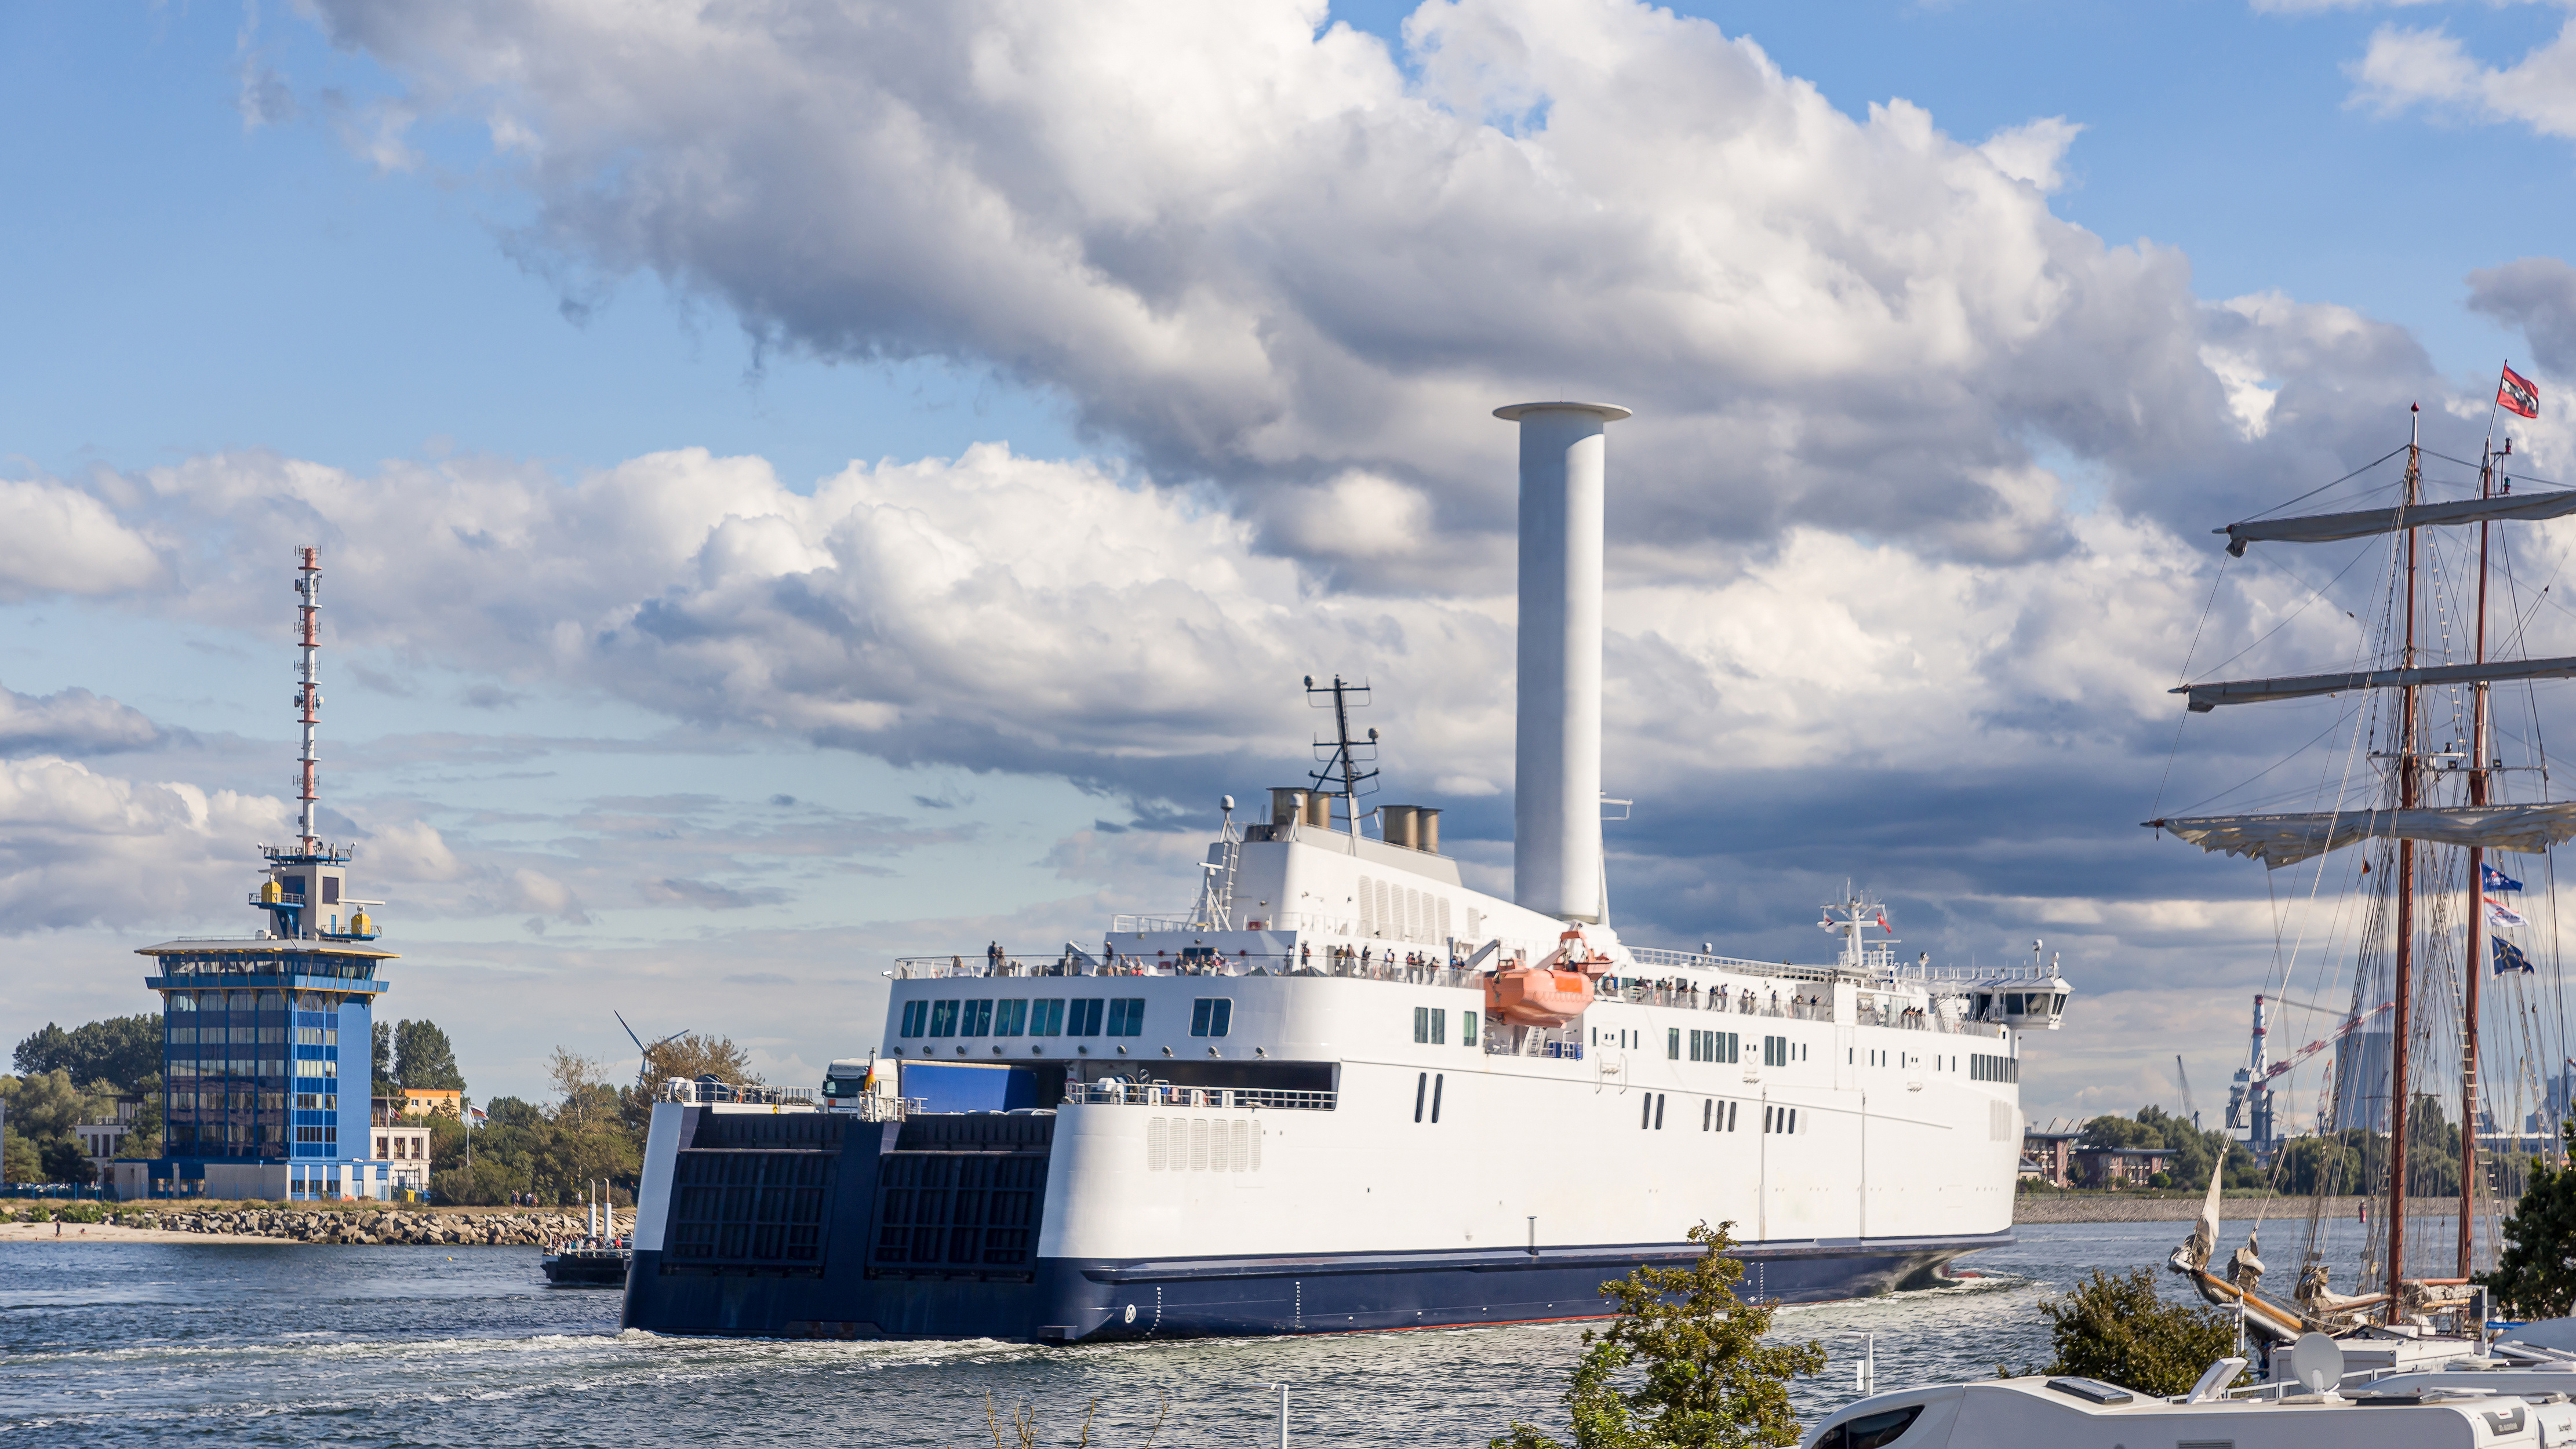
\includegraphics[width=0.7\textwidth]{FlettnerRotor.jpg}
    \caption[Schiff mit einem Flettner-Rotor.]{Schiff mit einem Flettner-Rotor.}
    \label{abb:kontmech_flettner}
  \end{figure}

\medskip
\hyperref[lsg:kontmech_magnus]{\textcolor{blue} {$\rightarrow$ L�sungsvorschlag}}.\\
%\href{FingerUeb1_AB.pdf#lsg:kontmech_magnus}{\textcolor{blue} {$\rightarrow$ L�sungsteil}}.\\

\noindent\rule[1ex]{\textwidth}{0.5pt}
\end{prob}

%-----------------------------------------------------------------------------------------------------------

\begin{prob} %�bung6
  \mittel{kontmech_SchiffKanal}{Kr�fte auf ein Schiff in einem Kanal}
	
    \begin{figure}
    \centering
    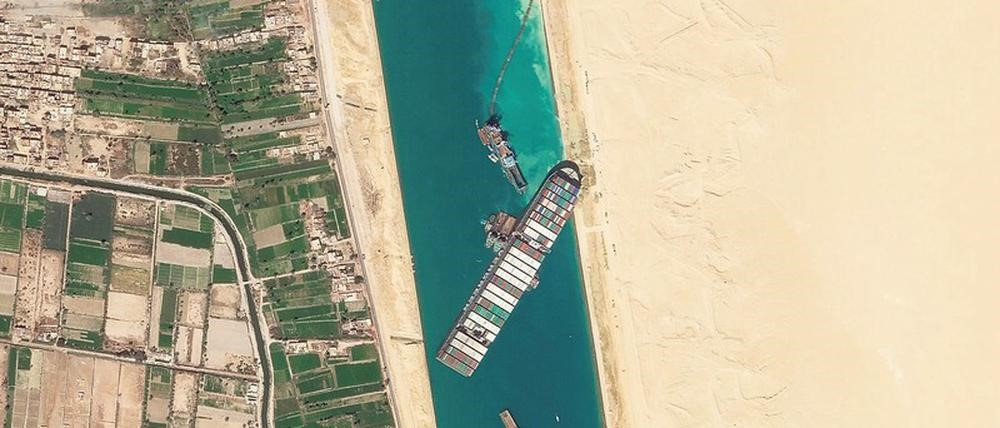
\includegraphics[width=0.5\textwidth]{EverGiven.jpg}
    \caption[Die Ever Given im Suez-Kanal 2021.]{Die Ever Given im Suez-Kanal 2021.}
    \label{abb:kontmech_SuzeKanalEverGiven}
  \end{figure}
	Das Containerschiff \textit{Ever Given} erlangte weltweite Bekanntheit als es am 23. M�rz 2021 im Suezkanal auf Grund lief, sich schr�g stellte und dadurch die Schifffahrtsrinne des Kanals sechs Tage lang blockierte. Wir wollen die Havarie etwas genauer untersuchen. Um zu bestimmen, welche Kr�fte durch den statischen Druck auf ein
  Schiff wirken, das in einem Kanal f�hrt, bedienen wir uns eines einfachen
  Modells. Es besteht aus dem Schiffsk�rper, der in
  \figref{kontmech_SchiffKanalAbmessungen} dargestellt ist.

  \begin{figure}
    \centering
    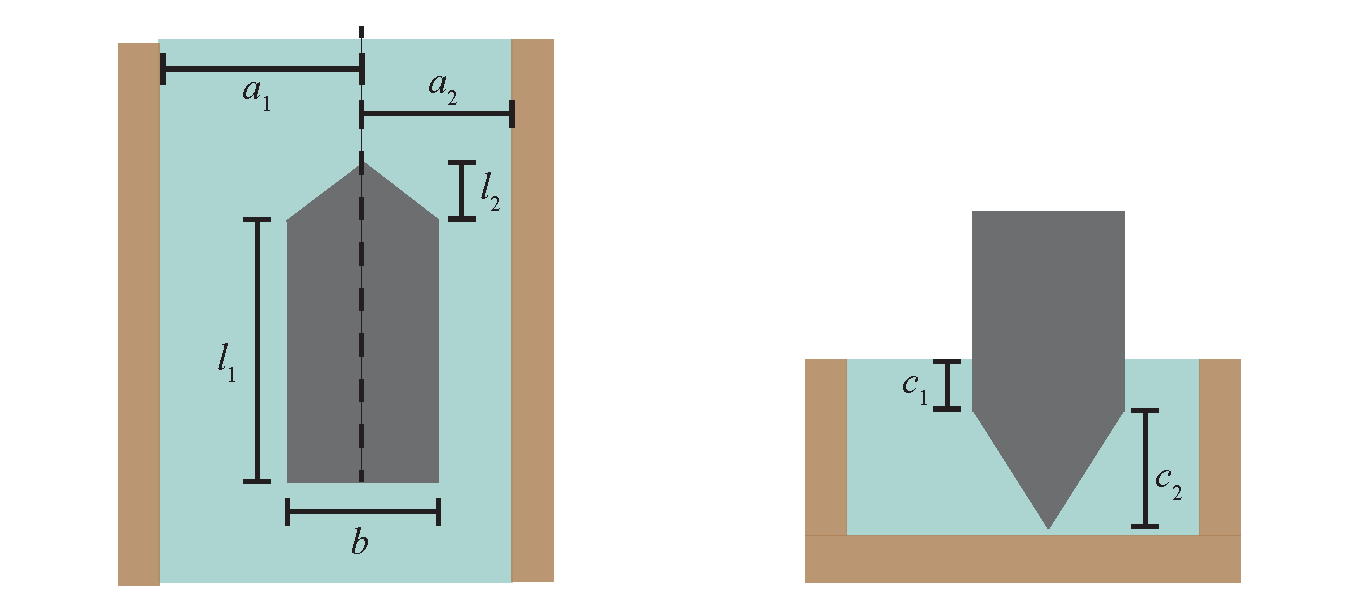
\includegraphics[width=\textwidth]{SchiffKanalAbm.pdf}
    \caption[Schiff in einem Kanal.]{Abmessungen eines Schiffs, das in einem
      Kanal f�hrt, um die darauf wirkenden Kr�fte zu bestimmen.}
    \label{abb:kontmech_SchiffKanalAbmessungen}
  \end{figure}

  Wir orientieren uns an Zahlen, die in der Gr��enordnung der Ever Given auf
  ihrer Fahrt im Suezkanal liegen \cite{Woehrbach2021}. Dazu nehmen wir ein
  Schiff der L�nge $l = \SI{400}{\metre}$, die sich auf $l_1 = \SI{380}
  {\metre}$ und $l_2 = \SI{20}{\metre}$ aufteilt, sowie der Breite $b =
  \SI{60}{\metre}$ an. Es hat einen Tiefgang von $c = \SI{16}{\metre}$ mit
  der Aufteilung $c_1 = \SI{6}{\metre}$ und $c_2 = \SI{10}{\metre}$. Der Kanal
  habe eine Breite von $a = \SI{200}{\metre}$. Das Schiff befahre ihn nicht auf
  der Mittellinie, sodass die Abst�nde zum Rand $a_1 = \SI{140}{\metre}$ und
  $a_2 = \SI{60}{\metre}$ betragen. Die Geschwindigkeit des Schiffes relativ
  zum Wasser liege etwas oberhalb von 10\,Knoten, also etwa $v_0=\SI{6}
  {\metre \per \second}$.

  Zur Berechnung nehmen wir vereinfacht an, dass das Schiff eine homogene
  Massendichte habe und das Wasser, das vom Schiff verdr�ngt wird, nur
  seitlich ausweicht und sich genau zur H�lfte auf beide Seiten des Schiffes
  aufteilt. Daraus ergeben sich links und rechts unterschiedliche
  Flie�geschwindigkeiten, die zu einem Unterschied im statischen Druck f�hren.
  Geben Sie die gesamte Kraft und das Drehmoment bez�glich des
  Massenmittelpunktes an.
  
  \medskip
\hyperref[lsg:kontmech_SchiffKanal]{\textcolor{blue} {$\rightarrow$ L�sungsvorschlag}}.\\
%\href{FingerUeb1_AB.pdf#lsg:kontmech_SchiffKanal}{\textcolor{blue} {$\rightarrow$ L�sungsteil}}.\\
\noindent\rule[1ex]{\textwidth}{0.5pt}
\end{prob}

%-----------------------------------------------------------------------------------------------------------

\begin{prob} %�bung7
  \einfach{kontmech_BarometrischeHoehenformel}{Barometrische H�henformel}
  Berechnen Sie die Druck- und Dichteverteilung in der Erdatmosph�re f�r
  den Fall einer rein statischen Atmosph�re. Gehen Sie dazu davon aus,
  dass nur die Gewichtskraftdichte
  \begin{equation*}
    \vec{f}_g = -\varrho g \veceZ
  \end{equation*}
  wirkt. Die notwendige Beziehung zwischen dem Druck und der Dichte l�sst
  sich aus der Zustandsgleichung idealer Gase der Thermodynamik
  \begin{equation*}
    p V = \nu R T
  \end{equation*}
  mit dem Druck $p$, dem Volumen $V$, der Stoffmenge $\nu$, der Gaskonstanten
  $R$ und der Temperatur $T$ gewinnen. Im Ergebnis erh�lt man die
  \glslink{baroHoeheBew}{barometrischen H�henformel}
  \index{H�henformel!barometrische|textbf}, die \iA von der Temperatur abh�ngen wird.
  Diesen komplizierteren Verlauf wollen wir hier jedoch nicht betrachten.

\medskip
\hyperref[lsg:kontmech_BarometrischeHoehenformel]{\textcolor{blue} {$\rightarrow$ L�sungsvorschlag}}.\\
%\href{FingerUeb1_AB.pdf#lsg:kontmech_BarometrischeHoehenformel}{\textcolor{blue} {$\rightarrow$ L�sungsteil}}.\\
\noindent\rule[1ex]{\textwidth}{0.5pt}
\end{prob}

%-----------------------------------------------------------------------------------------------------------

\begin{prob} %�bung8
\schwierig{kontmech_rotating_sprinkler}{Rotierender Rasensprinkler}	

\begin{enumerate} 
\item [a)] \textbf{Drehzahl}\\
Berechnen Sie die Drehgeschwindigkeit eines rotierenden Rasensprinklers (Rasensprengers) (\figref{kontmech_rotating_sprinkler}). Der Sprinkler hat eine Arml�nge $L$ und die beiden Ausstr�md�sen haben jeweils einen Durchmesser von $A_\text{D}$. Der Sprinkler kann sich frei drehen, zeigt aber eine Reibung, die in einem Drehmoment $\vec{M}_\text{Reibung}=\eta\,\vec{\omega}$ resultiert, welches von der Drehzahl \bzw der Rotationsfrequenz $\omega$ abh�ngt. Wir nehmen einen konstanten Wasserfluss von $Q$ an, zudem sei die Fl�ssigkeit inkompressibel und reibungsfrei. 
\item [b)] \textbf{Druck}\\
Berechnen Sie den notwendigen Druck am Wassereinlass als Funktion der Rotationsfrequenz $\omega$ und die daraus resultierende Reichweite.
\item [c)] \textbf{Blockierter Gartenschlauch}\\
Es ist eine allt�gliche Erfahrung, dass bei einer teilweisen Blockade des Wasseraustritts eines Gartenschlauchs, der Wasserstrahl weiter \bzw h�her schie�t. Warum ist das so? Geben Sie ohne Rechnung eine physikalische Erkl�rung. 
\end{enumerate}
          
\textbf{Zusatz }\\
Betrachten Sie auch das "`Anlaufverhalten"' des Rasensprinklers, indem Sie die Bewegungsgleichung \bzw die Bilanzgleichung f�r alle Drehimpulse des Systems auch f�r den nicht-station�ren Fall aufschreiben und numerisch l�sen. Was werden Sie beobachten? \\

	\begin{figure}
    \centering
    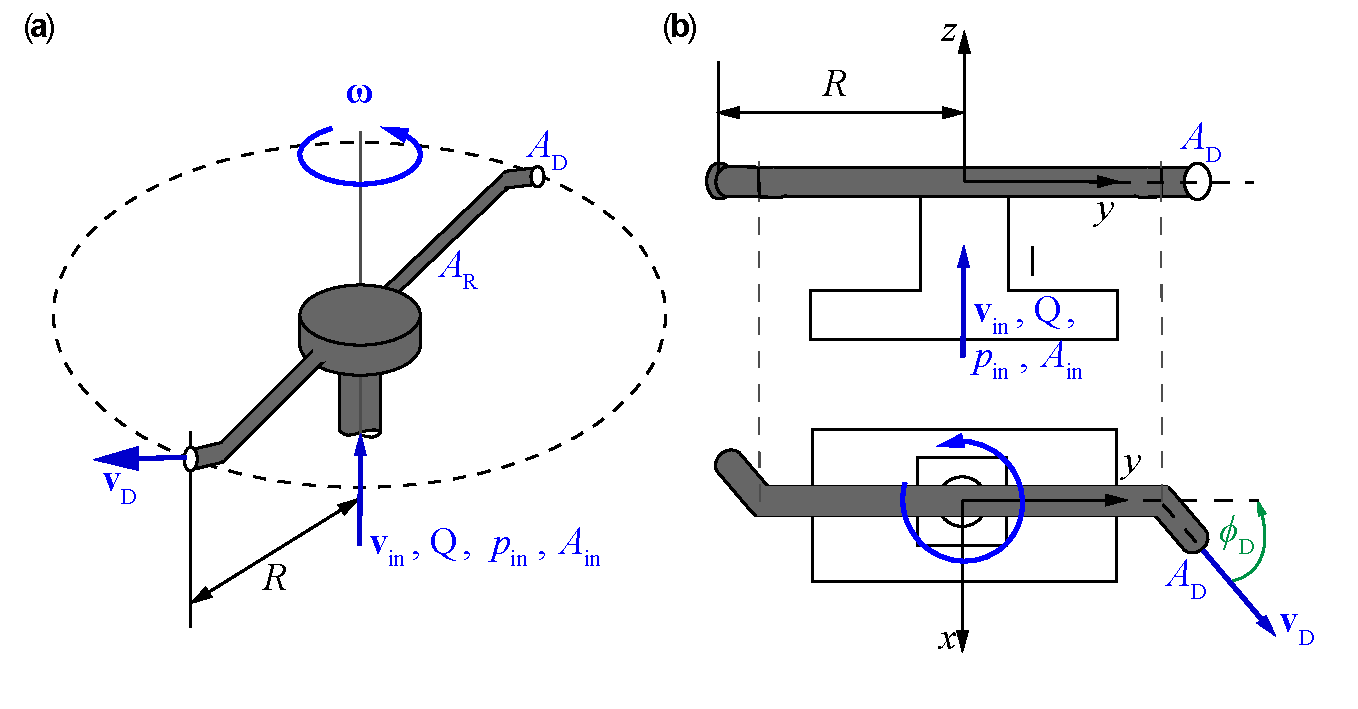
\includegraphics[width=\textwidth]{RegularSprinkler.pdf}
    \caption[Physik am Rasensprinkler.]{Physik am Rasensprinkler. \fa Prinzipaufbau und physikalische Gr��en. \b Geometrie. Die D�sen haben einen Winkel $\phi_\text{D}$ relativ zur Tangente des durch die horizontalen Arme definierten Kreises. }
    \label{abb:kontmech_rotating_sprinkler}
  \end{figure}

\medskip
\hyperref[lsg:kontmech_rotating_sprinkler]{\textcolor{blue} {$\rightarrow$ L�sungsvorschlag}}.\\
%\href{FingerUeb1_AB.pdf#lsg:kontmech_rotating_sprinkler}{\textcolor{blue} {$\rightarrow$ L�sungsteil}}.\\
\noindent\rule[1ex]{\textwidth}{0.5pt}
\end{prob}

%-----------------------------------------------------------------------------------------------------------
\newpage
\begin{prob} %�bung9
  \schwierig{kontmech_reverse_sprinkler}{Feynmans inverser Rasensprinkler}
  In seinem Buch \textit{"`Surely You're Joking, Mr. Feynman"'}%
  \footnote{Deutsche Ausgabe: "`Sie belieben wohl zu scherzen, Mr. Feynman."' (Piper 2018.)}
  \cite{Feynman1985} ver�ffentlichte Richard Feynman eine Episode zu einem
  Experiment, das den sp�ter nach ihm benannten\footnote{Tats�chlich war das
    Prinzip aber schon vor Feynman \ua von Ernst Mach \cite{Mach2012} erw�hnt
    worden.} inversen Rasensprinkler (\textit{Inverse Sprinkler} oder auch
  \textit{Reverse Sprinkler}) zum Gegenstand hatte.
  Feynman wollte in einem Experiment in seinem Labor in Princeton kl�ren, ob
  ein in einem Wassertank versenkter Rasensprinkler, der an eine Saugpumpe
  (\figref{kontmech_reverse_sprinkler}) angeschlossen war, sich entgegengesetzt
  zum normalen Betrieb (in Luft und mit Wasserdruck) dreht oder wie auch
  behauptet wurde, sich �berhaupt nicht dreht.\footnote{Das Experiment schlug
    �brigens fehl und endete in einem Chaos im Labor und Feynman hat sich bis
    zum Ende seines Lebens nie mehr �ffentlich zum Problem des
    \textit{Reverse Sprinklers} ge�u�ert.}

  Die Debatte �ber Feynmans inversen Rasensprinkler hat �ber Jahrzehnte die
  Gem�ter der Physiker erhitzt und es gibt in der Literatur dazu zahlreiche,
  zum Teil sich heftig widersprechende Abhandlungen dar�ber. 
	Eine Zusammenstellung findet sich \ua in \cite{Jenkins2004}.
  Im Internet zug�ngliche Videos zeigen sowohl rotierende als auch nicht
  rotierende Sprinkler.
  Es hat sich in letzter Zeit ein Konsensus herausgebildet \cite{Jenkins2004,
    Mungan2005, Rueckner2015, Beals2017}, dass ein Sprinkler in der exakten
  Auslegungsform nach \figref{kontmech_reverse_sprinkler} sich bis auf einen
  kurzen Moment beim Anschalten und Abschalten nicht bewegt.\\
\begin{figure}
    \centering
    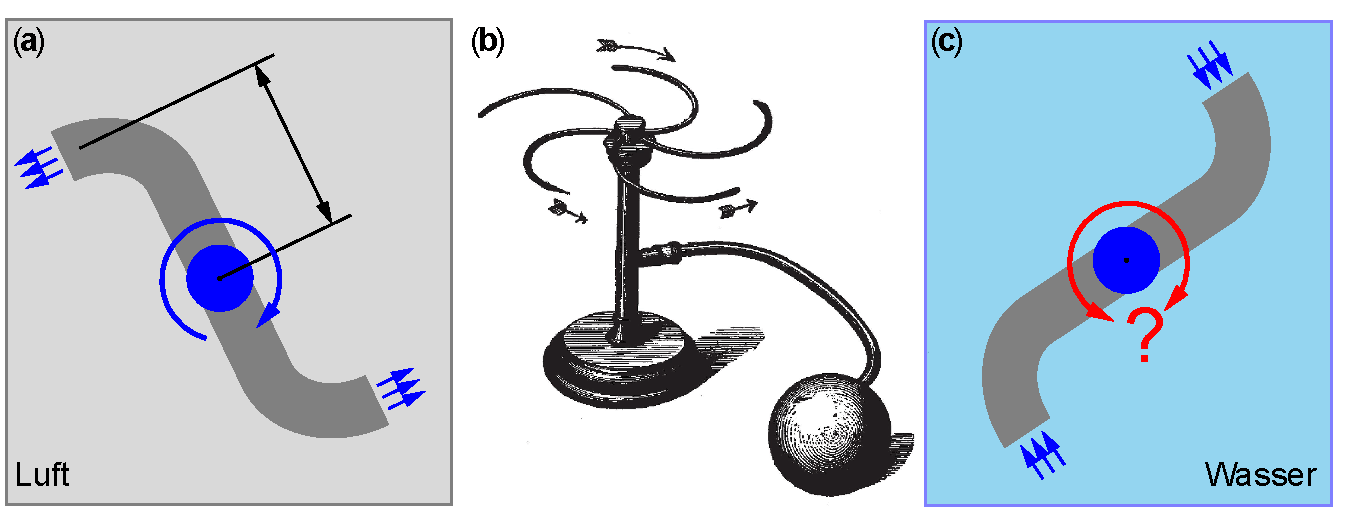
\includegraphics[width=\textwidth]{ReverseSprinkler.pdf}
    \caption[Feynmans inverser Rasensprinkler.]{Feynmans inverser Rasensprinkler. \fa Normaler Rasensprinkler mit Wasseraustritt in die Umgebungsluft.
		\fb Idee von Ernst Mach \cite{Mach2012} mit Saugvorrichtung an einem Rotationsrad \cite{Mach2012}. \fc Feynmans inverser Rasensprinkler in einem Wassertank eingetaucht.}
    \label{abb:kontmech_reverse_sprinkler}
\end{figure}
Begr�nden Sie diesen Konsensus und die entsprechenden experimentellen Befunde.
Beachten Sie dabei die spezielle Form der S- \bzw L-f�rmigen Konstruktion des
Sprinklers, bei der das abflie�ende Wasser genau im Drehpunkt nach unten
weg gesaugt wird. Unterscheiden Sie ferner zwischen der Anschaltphase und dem
station�ren Betrieb, starten Sie mit letzterem und betrachten Sie die
Drehimpulse und Drehmomente des Gesamtsystems aus Sprinkler, Wasser und
Wassertank.\\
Hinweis: Ber�cksichtigen Sie bei der Berechnung der Drehmomente zum einen die
Kraft, die durch den Wasserdruck im Rohr auf die Wand des Saugrohrarms des
Sprinklers am Punkt A durch den Wasserdruck $p_\text{R}$ im Rohr ausge�bt wird
und zum anderen die Wirkung des Druckverlustes bei einem Wasserdruck im Tank
$p_\text{T}$ zum Druck $p_\text{R}$ im Saugrohrarm.

\medskip
\hyperref[lsg:kontmech_reverse_sprinkler]{\textcolor{blue} {$\rightarrow$ L�sungsvorschlag}}.\\
%\href{FingerUeb1_AB.pdf#lsg:kontmech_reverse_sprinkler}{\textcolor{blue} {$\rightarrow$ L�sungsteil}}.\\
\noindent\rule[1ex]{\textwidth}{0.5pt}
\end{prob}

%-----------------------------------------------------------------------------------------------------------

\begin{prob} %�bung10
  \mittel{kontmech_StroemungRechteckrohr}{Str�mung durch Rohre}
  Berechnen Sie das Geschwindigkeitsprofil einer station�ren, laminaren
  Str�mung, die sich bei konstantem Druckgradienten f�r zwei Geometrien in
  einem Rohr ergibt. L�sen Sie dazu numerisch die partielle
  Differentialgleichung \eqref{eq:kontmech_NaStstat}, die sich als Spezialfall
  der Navier-Stokes-Gleichung ergibt.

  \begin{enumerate}
  \item L�sen Sie das zun�chst f�r ein kreisrundes Rohr und vergleichen
    Sie die numerische L�sung mit der analytischen, die in Beispiel
    \ref{bsp:kontmech_laminareStroemungen} in Kapitel
    \ref{kap:kontmech_laminareStroemungenFluessigkeiten} berechnet wurde.

  \item F�hren Sie dann die identische Rechnung f�r ein rechteckiges Rohr
    numerisch durch. Vergleichen Sie ihr Ergebnis mit der L�sung f�r das kreisrunde
    Rohr.
  \end{enumerate}
  
\medskip
\hyperref[lsg:kontmech_StroemungRechteckrohr]{\textcolor{blue} {$\rightarrow$ L�sungsvorschlag}}.\\
%\href{FingerUeb1_AB.pdf#lsg:kontmech_StroemungRechteckrohr}{\textcolor{blue} {$\rightarrow$ L�sungsteil}}.\\
\noindent\rule[1ex]{\textwidth}{0.5pt}
\end{prob}

%-----------------------------------------------------------------------------------------------------------
\begin{prob} %�bung11
  \schwierig{kontmech_StroemungTorricelli}{Gesetz von Torricelli - Str�mung aus einer Tonne}
Wir betrachten einen oben offenen, gro�en und gef�llten Beh�lter wie \zb eine Regentonne, die unten ein Loch hat.
Das Gesetz von Torricelli\footnote{Evangelista Torricelli (1608--1647) war ein italienischer Physiker und Mathematiker. Er wurde 1642 in Florenz der Nachfolger von Galileo Galilei als Hofmathematiker. Er arbeitete auf dem Gebiet der Physik der Gase und Fl�ssigkeiten und war an der Entwicklung der Infinitesimalrechnung beteiligt. 1644 entwickelte er das Quecksilberbarometer. Ihm zu Ehren wurde f�r lange Zeit die heute nicht mehr gebr�uchliche physikalische Ma�einheit f�r Luftdruck benannt: 1 Torr entsprach  $\SI{1}{\mm}$ Quecksilbers�ule.}\indexp{Torricelli, Evangelista}\index{Gesetz von Torricelli} besagt, dass die Austrittsgeschwindigkeit eines Wasserstrahls aus der �ffnung eines solchen Gef��es nur von der F�llh�he des Beh�lters abh�ngt, nicht von dessen Form und nicht von der Gr��e der �ffnung.\\
Erkl�ren Sie dieses der Intuition widersprechende Gesetz mit Hilfe der Bernoulli-Gleichung.
Berechnen Sie nun numerisch die Str�mungsverh�ltnisse in der Tonne nach \figref{kontmech_StroemungTorricelli} aus der \NVS \phantom{i}\eqref{eq:kontmech_NavierStokes}\index{Navier-Stokes-Gleichung}, wobei wir jetzt annehmen wollen, dass sich der Fl�ssigkeitsspiegel mit einer Geschwindigkeit $v_\text{S}$ nach unten bewegt und die Viskosit�t durch $\eta_\text{W}=\SI{1.0e-3}{\kg\per\metre\per\second}$ des Wassers \bzw $\eta_\text{Et}=\SI{1.2e-3}{\kg\per\metre\per\second}$ f�r Ethanol gegeben ist. Die Reynolds-Zahl ist durch $\mathrm{Re}=v_\text{S}\,H\,\varrho/\eta$ gegeben.\\
�berlegen Sie sich insbesondere sinnvolle Randbedingungen f�r $v_x(x=0),\,v_z(x=0),\, v_z(z=0)$ \usw \\
Berechnen Sie sowohl die Str�mungslinien als auch die Wirbellinien und stellen Sie diese graphisch dar.  (�bung nach \cite{Hoffmann2000}).\\
  \begin{figure}
    \centering
    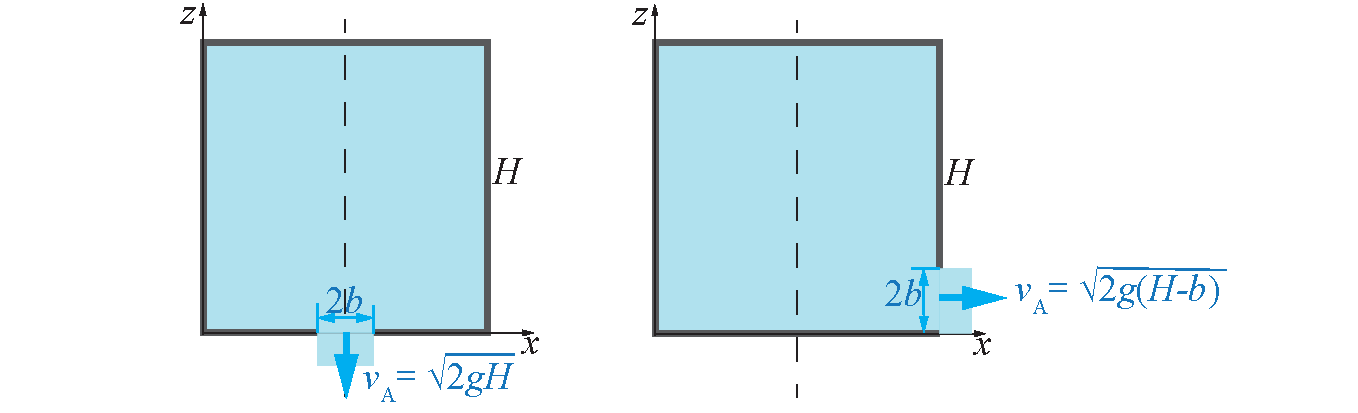
\includegraphics[width=\textwidth]{Torricelli.pdf}
    \caption[Gesetz von Torricelli.]{Gesetz von Torricelli. Str�mung aus einem Zylinder.}
    \label{abb:kontmech_StroemungTorricelli}
  \end{figure}

Wir wollen darauf hinweisen, dass es eine ganze Reihe ausgefeilter numerischer Pakete auf Basis der Finite-Differenzen-Methode\index{Finite Differenzen Methode} und anderer Methoden gibt, mit denen man komplexe Str�mungsprofile f�r ein breites Feld von Anwendungen von der Flugzeugtechnik bis zur Medizin berechnen kann. Wir empfehlen durchaus, dies mal mit einer Testversion auszuprobieren. \matlab{} bietet als Toolbox die \matlab{}  OpenFOAM and CFD Fluid Dynamics Toolbox
 unter \url{https://www.cfdtool.com} \bzw \url{https://www.mathworks.com/matlabcentral} (CFD Toolbox) an.\\
Als Beispiele f�r professionelle CFD Pakete mit Testversionen f�r Studenten seien genannt:\\
\url{https://www.ansys.com/de-de/products/fluids}\\
\url{https://www.simscale.com/product/cfd/}\\
Es ist und bleibt aber stets sehr instruktiv und immer eine Erlebnis, ein
Problem wie oben dargestellt, ausgehend von den Fundamentalgleichungen (hier
der \NVS) f�r einfache F�lle selbst zu programmieren und damit zu berechnen.
Im vorliegenden, zweidimensionalen Problem ist es lohnenswert, die
Stromfunktion $\vec{u}=u(x,y)\veceZ$ mit $\vec{v}=\rotv \vec{u}$ und den
Wirbelvektor $\vec{\Omega}=\Omega(x,y)\veceZ = 1/2\,\rotv \vec{v}$ einzuf�hren.
Die Navier-Stokes-Gleichung l�sst sich dann durch $u(x,y)$ und $\Omega(x,y)$
ausdr�cken. Dieses Problem l�sst sich in zwei gekoppelte, lineare
Gleichungssysteme aufspalten, die sich durch ein iteratives Verfahren,
\zb ein SOR-Verfahren, l�sen lassen.

\medskip
\hyperref[lsg:kontmech_StroemungTorricelli]{\textcolor{blue} {$\rightarrow$ L�sungsvorschlag}}.\\
%\href{FingerUeb1_AB.pdf#lsg:kontmech_StroemungTorricelli}{\textcolor{blue} {$\rightarrow$ L�sungsteil}}.\\
\noindent\rule[1ex]{\textwidth}{0.5pt}
\end{prob}

%-----------------------------------------------------------------------------------------------------------

\begin{prob} %�bung12
  \schwierig{kontmech_StroemungTank}{Str�mung durch einen Tank}
Nutzen Sie die \matlab-L�sungen von \probref{kontmech_StroemungTorricelli} und berechnen Sie aus der \NVS{} \eqref{eq:kontmech_NavierStokes} die Str�mung f�r einen Durchfluss durch einen Beh�lter nach \figref{kontmech_StroemungTank}. (Dies stellt eine Variation des Gesetzes von Torricelli dar.) Nehmen Sie zun�chst $B=H$ und $a=b$ an und berechnen Sie wiederum die Str�mungslinien und Wirbellinien und stellen Sie diese graphisch dar. (Idee zur �bung nach \cite{Hoffmann2000}. Siehe auch Bemerkungen in \probref{kontmech_StroemungTank}.)

  \begin{figure}
    \centering
    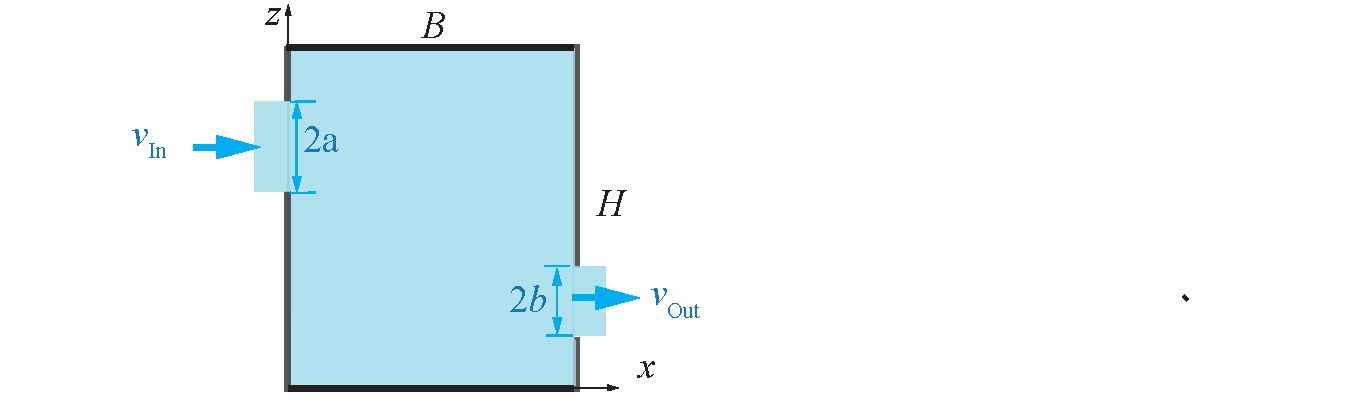
\includegraphics[width=\textwidth]{Tankdurchfluss.pdf}
    \caption[Str�mung durch einen Tank.]{Str�mung durch einen Tank.}
    \label{abb:kontmech_StroemungTank}
  \end{figure}

\medskip
\hyperref[lsg:kontmech_StroemungTank]{\textcolor{blue} {$\rightarrow$ L�sungsvorschlag}}.\\
%\href{FingerUeb1_AB.pdf#lsg:kontmech_StroemungTank}{\textcolor{blue} {$\rightarrow$ L�sungsteil}}.\\
\noindent\rule[1ex]{\textwidth}{0.5pt}
\end{prob}


%-----------------------------------------------------------------------------------------------------------

\newpage
\begin{prob} %�bung13
\einfach{kontmech_IdealerWirbel}{Idealer Wirbel}
H�ufig nehmen Wirbel in str�menden Fl�ssigkeiten im Inneren eine nahezu ideale
Form an. Ein idealer Wirbel besteht aus einem Wirbelkern, in dem die
Winkelgeschwindigkeit konstant ist. Nach einem recht schmalen �bergangsbereich
liegt eine Str�mung mit konstanter Umlaufgeschwindigkeit vor. Berechnen
Sie f�r diese beiden Bereiche den Wirbelvektor und die Zirkulation. Zeigen
Sie an diesem Beispiel die G�ltigkeit der Beziehung
\eqref{eq:kontmech_ZirkulationWirbelvektor}.

\medskip
\hyperref[lsg:kontmech_IdealerWirbel]{\textcolor{blue} {$\rightarrow$ L�sungsvorschlag}}.\\
%\href{FingerUeb1_AB.pdf#lsg:kontmech_IdealerWirbel}{\textcolor{blue} {$\rightarrow$ L�sungsteil}}.\\

\noindent\rule[1ex]{\textwidth}{0.5pt}
\end{prob}

%-----------------------------------------------------------------------------------------------------------

\begin{prob} %�bung14
\schwierig{kontmech_UmformungWirbelsatz}{Helmholtzscher Wirbelsatz}
Zeigen Sie, dass f�r die Umformung der Navier-Stokes-Gleichung folgende Beziehung gilt:
\begin{equation}
  \rotv \lk \lk \vec{v} \cdot \gradv \rk \vec{v} \rk
  = \rotv \lk \rotv \vec{v} \times \vec{v} \rk \,. \label{eq:kontmech_umformumg_NSG}
\end{equation}

\medskip
\hyperref[lsg:kontmech_UmformungWirbelsatz]{\textcolor{blue} {$\rightarrow$ L�sungsvorschlag}}.\\
%\href{FingerUeb1_AB.pdf#lsg:kontmech_UmformungWirbelsatz}{\textcolor{blue} {$\rightarrow$ L�sungsteil}}.\\
\noindent\rule[1ex]{\textwidth}{0.5pt}
\end{prob}

%-----------------------------------------------------------------------------------------------------------

\begin{prob} %�bung15
\mittel{kontmech_fluesse}{Ist der Rhein laminar oder turbulent?}
Sch�tzen Sie ab, ob der Rhein von K�ln nach D�sseldorf laminar oder turbulent flie�t.\\
K�nnen Sie eine N�herungsformel f�r Gew�sser herleiten? F�gen Sie in der Formel einen Proportionalit�tsfaktor $\gamma$ f�r die Rauigkeit des Bodens des Gew�ssers ein, mit $\gamma = 1 $ f�r ideal glatte Oberfl�che und $\gamma \gg 1 $ f�r raue Oberfl�chen, wie \zb ein Kiesbett.\\

\medskip
\hyperref[lsg:kontmech_fluesse]{\textcolor{blue} {$\rightarrow$ L�sungsvorschlag}}.\\
%\href{FingerUeb1_AB.pdf#lsg:kontmech_fluesse}{\textcolor{blue} {$\rightarrow$ L�sungsteil}}.\\

\noindent\rule[1ex]{\textwidth}{0.5pt}
\end{prob}

%-----------------------------------------------------------------------------------------------------------
\begin{prob} %�bung16
  \schwierig{kontmech_StokesReibung}{Stokes-Reibung}\index{Stokes-Reibung}
  Leiten Sie aus der Navier-Stokes-Gleichung die Beziehung 
  \indexp{Stokes, Sir George Gabriel}
  \begin{align}
    \vec{F_\text{R}} = - 6\,\pi\,\eta\,R_0\,v\,\frac{\vec{v}}{\left|\vec{v}\right|}  \label{eq:kontmech_StokesReibungKugel}
  \end{align}
  f�r die sogenannte Stokes-Reibungskraft in einer viskosen Fl�ssigkeit
  (Viskosit�t $\eta$) auf kugelf�rmige K�rper (Radius $R_0$) her. Die
  Bedingungen, unter denen wir die Stokes-Reibung vorfinden, sind:
  \begin{itemize}
  \item kleine Reynolds-Zahl ($\ll 1$), 
  \item hohe Reibung,
  \item vernachl�ssigbare Tr�gheitskr�fte in der umstr�menden Fl�ssigkeit.
  \end{itemize}
  
\medskip
\hyperref[lsg:kontmech_StokesReibung]{\textcolor{blue} {$\rightarrow$ L�sungsvorschlag}}.\\
%\href{FingerUeb1_AB.pdf#lsg:kontmech_StokesReibung}{\textcolor{blue} {$\rightarrow$ L�sungsteil}}.\\

\noindent\rule[1ex]{\textwidth}{0.5pt}
\end{prob}


% ----------------------------------------------------------------------------------------------------------
% ----------------------------------------------------------------------------------------------------------
\newpage
\subsection{�bungen zur Dynamik deformierbarer, fester K�rpern}

\medskip

% -----------------------------------------------------------------------------------------------------------

\begin{prob} %�bung17
  \mittel{kontmech_WelleSaite}{Fortschreitende Welle auf der eingespannten
    Saite}
  Fertigen Sie analog zum Vorgehen aus Beispiel
  \ref{bsp:kontmech_finiteDiffSaite} ein Programm an, das folgende
  laufenden Wellen auf einer an beiden Enden eingespannten Saite f�r mehrere
  Zeitschritte berechnet.
  \begin{enumerate}
  \item Ein St�rung in Form eines Gau�-Pakets, das sich, ohne sich zu verformen,
    auf der Saite bewegt.
  \item Eine Welle, die dadurch entsteht, dass eines der eingespannten Enden
    periodisch (sinusf�rmig) auf und ab bewegt wird.
  \end{enumerate}

  \medskip
  \hyperref[lsg:kontmech_WelleSaite]{\textcolor{blue} {$\rightarrow$ L�sungsvorschlag}}.\\
  %\href{FingerUeb1_AB.pdf#lsg:kontmech_WelleSaite}{\textcolor{blue} {$\rightarrow$ L�sungsteil}}.\\
\noindent\rule[1ex]{\textwidth}{0.5pt}
\end{prob}

% -----------------------------------------------------------------------------------------------------------

\begin{prob} %�bung18
  \schwierig{kontmech_AchterbahnKont}{Achterbahn-Bewegungsgleichungen im kontinuierlichen Ansatz}
  Bilden Sie den Kontinuums-Grenzwert des Ansatzes aus
  \probref{bew_achterbahn_diskret}, in der ein Zug auf einer Achterbahn aus
  Punktmassen gebildet wurde, die �ber Federn miteinander verbunden sind.
  Dadurch geht der Zug in ein kontinuierliches Band �ber, das in Erweiterung
  der Darstellung aus Kapitel \ref{kap:rollercoaster} jedoch elastisch
  ist.

  Gehen Sie von einer allgemeinen Beziehung $z=h(x)$ aus und zeigen Sie,
  dass mit den Bezeichnungen, die in Kapitel \ref{kap:kontmech_festLagrange}
  f�r die schwingende Saite eingef�hrt wurden, die Bewegungsgleichung
  \begin{equation}
    \frac{\partial^2 x}{\partial t^2} = -\frac{h'(x)h''(x)}{1 + h'(x){}^2}
    \lk \frac{\partial x}{\partial t} \rk^2
    - \frac{g h'(x)}{1 + h'(x){}^2}
    +\frac{\Phi}{\varrho_L}\, \frac{h'(x)h''(x)}{1 + h'(x){}^2} \lk
    \frac{\partial x}{\partial l} \rk^2
    + \frac{\Phi}{\varrho_L}\, \frac{\partial^2 x}{\partial l^2}
    \label{eq:kontmech_DGLAchterbahnzug}
  \end{equation}
  lautet.
  
  \medskip
  \hyperref[lsg:kontmech_AchterbahnKont]{\textcolor{blue} {$\rightarrow$ L�sungsvorschlag}}.\\
  %\href{FingerUeb1_AB.pdf#lsg:kontmech_AchterbahnKont}{\textcolor{blue} {$\rightarrow$ L�sungsteil}}.\\

\noindent\rule[1ex]{\textwidth}{0.5pt}
\end{prob}


% -----------------------------------------------------------------------------------------------------------

\begin{prob} %�bung19
  \mittel{kontmech_AchterbahnZug}{Elastischer Achterbahnzug auf einer
    Gau�kurven-Strecke}
  Stellen Sie ein Programm zur numerischen L�sung der partiellen
  Differentialgleichung \eqref{eq:kontmech_DGLAchterbahnzug} eines
  elastischen, kontinuierlichen Zuges auf einer Achterbahnstrecke auf.
  Gehen Sie wie in \probref{bew_achterbahn} von einer Gau�kurve als
  Achterbahnstrecke aus. Als numerisches L�sungsverfahren k�nnen Sie
  die Methode der finiten Differenzen w�hlen und sich an Beispiel
  \ref{bsp:kontmech_finiteDiffSaite} orientieren.

  \medskip
  \hyperref[lsg:kontmech_AchterbahnZug]{\textcolor{blue} {$\rightarrow$ L�sungsvorschlag}}.\\
  %\href{FingerUeb1_AB.pdf#lsg:kontmech_AchterbahnZug}{\textcolor{blue} {$\rightarrow$ L�sungsteil}}.\\
\noindent\rule[1ex]{\textwidth}{0.5pt}
\end{prob}


% -----------------------------------------------------------------------------------------------------------

\begin{prob} %�bung20
  \mittel{kontmech_AchterbahnBeschleunigungen}{Normalbeschleunigung eines
    Fahrgastes im Achterbahnzug}
  Stellen Sie die Gleichungen f�r die Normalbeschleunigung auf, die auf einen
  Fahrgast im Achterbahnzug wirkt. Gehen
  Sie dabei von dem aus \probref{kontmech_AchterbahnZug} vorliegenden
  numerischen Bahnverlauf aus und ber�cksichtigen Sie wie im diskreten Modell
  aus \probref{bew_achterbahn_diskret}, dass auf die Fahrg�ste die Schwere- und
  die Radialbeschleunigung wirken. Vernachl�ssigen Sie analog zum diskreten
  Modell die Federkr�fte, da die F�hrg�ste in tangentialer Richtung nicht
  fest mit dem Wagen verbunden sind. Werten Sie die Normalbeschleunigungen aus
  und tragen Sie diese zusammen mit ihren $x$- und $z$-Komponenten �ber dem
  Bahnverlauf auf.
  
  \medskip
  \hyperref[lsg:kontmech_AchterbahnBeschleunigungen]{\textcolor{blue} {$\rightarrow$ L�sungsvorschlag}}.\\
  %\href{FingerUeb1_AB.pdf#lsg:kontmech_AchterbahnBeschleunigungen}{\textcolor{blue} {$\rightarrow$ L�sungsteil}}.\\
\noindent\rule[1ex]{\textwidth}{0.5pt}
\end{prob}

% -----------------------------------------------------------------------------------------------------------

\begin{prob} %�bung21
  \einfach{kontmech_ElastizitaetTorsion}{Elastizit�ts-/Torsionsmodul im
    dreidimensionalen Spannungstensor}
  Verifizieren Sie, dass Sie im dreidimensionalen Spannungstensor nach
  Gleichung \eqref{eq:kontmech_Spannungstensor1} die Beziehungen
  \eqref{eq:kontmech_Elastizitaetsmodul4} f�r das Elastizit�tsmodul und
  \eqref{eq:kontmech_Torsionsmodul3} f�r das Torsionsmodul erhalten. Gehen
  Sie f�r letzteres wieder von der Kleinwinkeln�herung aus.
  
  \medskip
  \hyperref[lsg:kontmech_ElastizitaetTorsion]{\textcolor{blue} {$\rightarrow$ L�sungsvorschlag}}.\\
  %\href{FingerUeb1_AB.pdf#lsg:kontmech_ElastizitaetTorsion}{\textcolor{blue} {$\rightarrow$ L�sungsteil}}.\\
\noindent\rule[1ex]{\textwidth}{0.5pt}
\end{prob}

% -----------------------------------------------------------------------------------------------------------

\begin{prob} %�bung22
  \schwierig{kontmech_BogenSpannung}{Bogen mit Spannung durch eine Saite}
  Wir betrachten einen Bogen, der durch eine Seite gespannt ist (siehe
  \figref{kontmech_UebungBogen}).
  \begin{figure}
    \centering
    
\includegraphics[width=\textwidth]{BogenAufbau.pdf}
    \caption[Bogen gespannt mit einer Saite]{Bogen, der mit einer
      Seite gespannt ist. Die Kr�mmung in der Ruhelage wird durch den
      Winkel $\theta$ beschrieben.}
    \label{abb:kontmech_UebungBogen}
  \end{figure}
  In Abh�ngigkeit von der Kr�mmung in der Ruhelage, die durch den Winkel
  $\theta$ gegeben ist, l�sst sich mit dem Elastizit�tsmodul $E$, dem
  Fl�chentr�gheitsmoment $I$, der Masse $M$ des Bogens, seiner L�nge $L$,
  der externen Spannkraft pro L�nge $F_l$ und der Koordinate $s$ entlang
  des Bogens die Bewegungsgleichung f�r eine Auslenkung $n$ aus der Ruhelage
  aufstellen \cite{Cross2001}:
  \begin{equation*}
    \frac{M}{L} \frac{\partial^2 n}{\partial t^2} = F_l - E I\,
    \frac{\partial^4 n}{\partial s^2}
  \end{equation*}
  F�r eine numerische L�sung diskretisieren wir den Bogen in $N$ Elemente,
  f�hren die Masse $m=M/N$ und die L�nge $h=L/N$ eines Elements sowie die
  Spannkraft $F=F_l h$ auf ein Element ein und multiplizieren mit diesem $h$,
  was auf die Gleichung
  \begin{equation*}
    m \frac{\partial^2 n}{\partial t^2} = F - E I h\,
    \frac{\partial^4 n}{\partial s^2}
  \end{equation*}
  f�hrt. Unter der Annahme einer harmonischen Schwingung gewinnen wir daraus
  die gew�hnliche Differentialgleichung 4. Ordnung
  \begin{equation*}
    \frac{\partial^4 n}{\partial s^2} = 
    \frac{m \omega^2}{E I h} n + \frac{F}{E I h} \; ,
  \end{equation*}
  f�r die die Randbedingungen $\partial^2n/\partial s^2 = \partial^3n/
  \partial s^3 = 0$ im Fall eines freien Endes gelten \cite{Cross2001}. Dies
  entspricht auch der betrachteten Modellierung. Die externe Kraft wirkt nur
  an den Punkten, an denen die gespannte Saite befestigt ist. Dort kann sie
  durch
  \begin{equation}
    F= T_1 \cos(\vartheta)\,\frac{\partial n}{\partial s} - 2k\,n\,
    \sin^2(\vartheta)
  \end{equation}
  mit der Spannkraft $T_1$ in der Ruhelage und der Federkonstanten $k$
  der Saite beschrieben werden.
  
  L�sen Sie die Differentialgleichung numerisch f�r verschiedene Winkel
  $\vartheta$. Zeigen Sie damit, dass f�r kleine Winkel die Schwingungsfrequenz
  $f = \omega/(2\pi)$ kleiner ist als f�r den Bogen ohne Seite, f�r
  zunehmenden Winkel aber ansteigt und deutlich gr��er werden kann als
  im Fall ohne spannende Saite. Verwenden Sie die folgenden Materialparameter
  f�r den Aluminiumbogen aus \cite{Cross2001}: $EI = \SI{3{,}09}{\kilo\gram\,
    \metre^2}$, $M = \SI{118}{\gram}$, $L = \SI{52}{\centi\metre}$, $k =
  \SI{2{,}1e4}{\newton\per\metre}$.

  F�r die numerische L�sung ist es empfehlenswert, von einer festen
  Intervallzahl $N$ auszugehen und die Spannkraft in zwei Intervallen
  nahe, jedoch nicht exakt am Rand (freies Ende) anzusetzen, ansonsten
  verschwindet sie \cite{Cross2001,Cross1999}. Neben den gegebenen
  Randbedingungen lauten die zwei verbleibenden Startbedingungen $n(0) = n_a$
  mit einem beliebigen $n_a$ (lineare Differentialgleichung) und
  $\partial n(0)/\partial s = n'_a$. In einer Nullstellensuche bestimmt man
  $n'_a$ und $\omega$ so, dass die Bedingungen auch am anderen Ende des Bogens
  erf�llt sind. Man muss darauf achten, dass die Spannkraft der Saite immer
  in die richtige Richtung angesetzt wird. 
  
	Es ist interessant, dass obwohl der Rahmen eines Saiteninstruments beim Einlegen der Saiten einer gro�en Spannkraft unterliegt, dieser durch das Anbringen mehrerer Saiten nicht versteift wird. Hingegen wird ein Bogen, wie wir ihn gerade beschrieben haben, viel steifer, wenn er bespannt ist. Ein Tennisschl�ger - �hnlich wie ein Saiteninstrument - wird eher weicher, wenn die Saiten hinzugef�gt werden. Die Erkl�rung ist, dass durch die Bespannung die Modenfrequenzen f�r Querschwingungen bei einem Bogen zunehmen und bei einem Schl�ger abnehmen. Die Wirkung der Saiten h�ngt also von der Art der Biegung des Rahmens im Zustand ohne Bespannung ab \cite{Cross2001}.
	
  \medskip
  \hyperref[lsg:kontmech_BogenSpannung]{\textcolor{blue} {$\rightarrow$ L�sungsvorschlag}}.\\
  %\href{FingerUeb1_AB.pdf#lsg:kontmech_BogenSpannung}{\textcolor{blue} {$\rightarrow$ L�sungsteil}}.\\
\noindent\rule[1ex]{\textwidth}{0.5pt}
\end{prob}

% -----------------------------------------------------------------------------------------------------------

\begin{prob} %�bung23
  \schwierig{kontmech_Chladni}{Chladnische Klangfiguren}
  Stellen Sie die Differentialgleichung f�r eine d�nne, elastische Scheibe
  auf, die zu Deformationsschwingungen in der Form f�hig ist, dass die
  Schwingungsamplitude senkrecht zur Scheibenfl�che ist. Finden Sie mit einem
  numerischen L�sungsverfahren f�r partielle Differentialgleichungen einige
  Eigenmoden f�r eine Scheibe, die
  \begin{enumerate}
  \item eine Kreisform,
  \item eine quadratische Form,
  \item eine Rechteckform mit unterschiedlichen Kantenl�ngen
  \end{enumerate}
  hat.
  
  \medskip
  \hyperref[lsg:kontmech_Chladni]{\textcolor{blue} {$\rightarrow$ L�sungsvorschlag}}.\\
  %\href{FingerUeb1_AB.pdf#lsg:kontmech_Chladni}{\textcolor{blue} {$\rightarrow$ L�sungsteil}}.\\
\noindent\rule[1ex]{\textwidth}{0.5pt}
\end{prob}


% ----------------------------------------------------------------------------------------------------------
% ----------------------------------------------------------------------------------------------------------

\newpage
\subsection{�bungen zu Wellen}

\medskip

% ----------------------------------------------------------------------------------------------------------

\begin{prob} %�bung24
  \mittel{kontmech_Dispersion}{Wellenausbreitung und Dispersion}
Wir wollen L�sungen einer sich linear ausbreitenden, fortlaufenden Welle, der allgemeinen Form
\begin{equation}
 \psi(t,x) = f(\omega t \pm kx) \label{eq:kontmech_fortl_welle01}
\end{equation}
berechnen. Hierin sind $k$ als Wellenzahl und $\omega$ als Kreisfrequenz definiert. Durch Einsetzen in die Wellengleichung \eqref{eq:kontmech_PDGLSaite2} ergab sich die \gls{Dispersionsrelation}\index{Dispersionsrelation} 
\begin{equation}
  \omega = \sqrt{\frac{E}{\varrho}}\,k = v_\text{Ph}\,k ~~~~\text{mit}~~v_\text{Ph} = \sqrt{\frac{E}{\varrho}} \,.
  \label{eq:kontmech_DispersionsRel02}
\end{equation}
Hierin ist $v_\text{Ph}$ die \textit{Phasengeschwindigkeit}\index{Phasengeschwindigkeit}, die als Ausbreitungsgeschwindigkeit gleicher Phasen anzusehen ist.
Allgemeiner gilt f�r Dispersionsrelationen $\omega = \omega(k)$ \bzw $v_\text{Ph} = v_\text{Ph}(k)$, womit man dann
die \textit{Gruppengeschwindigkeit}\index{Gruppengeschwindigkeit}
\begin{equation}
  v_\text{Gr} = \frac{\D \omega(k)}{\D k}  \label{eq:kontmech_DispersionsRel04}
\end{equation}
definieren kann, die die Geschwindigkeit ist, mit der sich die Amplitudeneinh�llende eines Wellenpakets fortbewegt. F�r verlustfreie Medien kann diese auch als die Geschwindigkeit der Signal(Energie)-�bertragung verstanden werden.\\
Eine einfache Rechnung (Kettenregel) ergibt einen Zusammenhang zwischen Phasen- und Gruppengeschwindigkeit:
\begin{equation}
  v_\text{Gr} = \frac{\D \omega(k)}{\D k} = \frac{(\D v_\text{Ph}\,k)}{\D k} = v_\text{Ph} + k \frac{\D v_\text{Ph}(k)}{\D k} = v_\text{Ph} - \lambda \frac{\D v_\text{Ph}(\lambda)}{\D \lambda}\,, \label{eq:kontmech_DispersionsRel05}
\end{equation}
wobei wir im letzten Schritt die Wellenzahl $k$ durch die Wellenl�nge $\lambda = 1/k$ ersetzt haben. Wenn die Phasengeschwindigkeit nicht von der Wellenl�nge \bzw Wellenzahl abh�ngt, dann sind Phasengeschwindigkeit und Gruppengeschwindigkeit gleich. Ist $v_\text{Ph} > v_\text{Gr} $ so zeigt das Material, in dem sich die Welle ausbreitet, \textit{normale Dispersion}\index{Dispersion!normale}, im Fall von  $v_\text{Ph} < v_\text{Gr}$ \textit{anormale Dispersion}.\index{Dispersion!anormale}
\begin{enumerate}
\item Berechnen Sie die �berlagerung zweier Wellen der Form $\psi_i(x,t) = \cos(k_i\,x - \omega_i\,t)$ mit $i=1,2$, die sich in Medien mit drei unterschiedlichen Dispersion ausbreiten: $v_\text{Gr}  = 0.5\, v_\text{Ph}$ und $v_\text{Gr}  = 1.5, v_\text{Ph}\,.$ 
\item Wiederholen Sie die Rechnung f�r �berlagerung zweier gegeneinander laufender Wellen der Form $\psi_i(x,t) = \cos(k_i\,x - (-1)^i\,\omega_i\,t)$ mit $i=1,2$. 
\item �berlagern Sie nun numerisch eine gro�e Zahl $N \approx 50$ von Wellen der Form $\psi_i(x,t) = \cos(k_i\,x - \omega_i\,t)$ mit $i=-N,N$. 
Wir erhalten ein Wellenpaket. 
Wir wollen eine lineare normale Dispersion wie folgt annehmen:
\begin{align}
	  v_\text{Ph}(k_i) = v_{\text{Ph},0} + v_\text{d}\; \frac{\left|k_i\right|-k_0}{k_0} \,. \label{eq:kontmech_DispersionsRel06}
\end{align}
Die Konstante $v_\text{d}$ hat ebenfalls die Dimension einer Geschwindigkeit und ist f�r normale Dispersion negativ, damit \eqref{eq:kontmech_DispersionsRel05} erf�llt ist, $v_{\text{Ph},0}$ ist die Phasengeschwindigkeit und $k_0$ die Wellenzahl f�r die Mittenwellenl�nge $\lambda_0 = 1/k_0$.
Die Gruppengeschwindigkeit f�r diese Mittenwellenl�nge ist $v_{\text{Gr},0} = v_{\text{Ph},0} + v_\text{d}\,$.
Beschreiben Sie das Verhalten des Wellenpaketes.\\
\end{enumerate}
\hyperref[lsg:kontmech_Dispersion]{\textcolor{blue} {$\rightarrow$ L�sungsvorschlag}}.\\
  %\href{FingerUeb1_AB.pdf#lsg:kontmech_Dispersion}{\textcolor{blue} {$\rightarrow$ L�sungsteil}}.\\
\noindent\rule[1ex]{\textwidth}{0.5pt}
\end{prob}

% ----------------------------------------------------------------------------------------------------------
\newpage
\begin{prob} %�bung25
  \schwierig{kontmech_Dispersion2}{Ausbreitung eines Wellenpakets unter Dispersion}
Wir betrachten in Erweiterung von \probref{kontmech_Dispersion} ein sich ausbreitendes Wellenpaket mit einer Gau�-f�rmigen Amplitudeneinh�llenden: 
\begin{equation}
 \psi(t,x) = A_0\,\e^{-t^2/\tau_\text{P}{}^2}\, \mathrm{exp}\lek{\im (k_0\,x - \omega_0\,t + \varphi(t))}\rek\,\label{eq:kontmech_DispersionsRel07}
\end{equation}
worin $\tau_\text{P}$ eine Zeitkonstante ist, die die Ausdehnung des Wellenpaketes beschreibt und $\varphi(t)$ eine m�gliche zeitabh�ngige Phase, die zu Beginn $\varphi =0$ ist.
Dieses Wellenpaket durchl�uft nun ein dispersives Medium. Die Dispersion soll wie in \probref{kontmech_Dispersion} durch
\begin{align}
   v_\text{Gr} = v_\text{Ph} + k \frac{\D v_\text{Ph}(k)}{\D k} = v_\text{Ph} - \lambda \frac{\D v_\text{Ph}(\lambda)}{\D \lambda}\,, \label{eq:kontmech_DispersionsRel08}
\end{align}
beschrieben werden.

Wir definieren noch die instantane Frequenz, die als zeitliche Ableitung der Phase des Wellenpaketes definiert ist:
\begin{align*}
   \omega_i(t) = \omega_0 + \frac{\D \varphi}{\D t} \,.
\end{align*}
Offensichtlich gilt f�r unser Wellenpaket vor Eintritt in das dispersive Medium $\omega_i(t) = \omega_0$.

  \begin{figure}
    \centering
    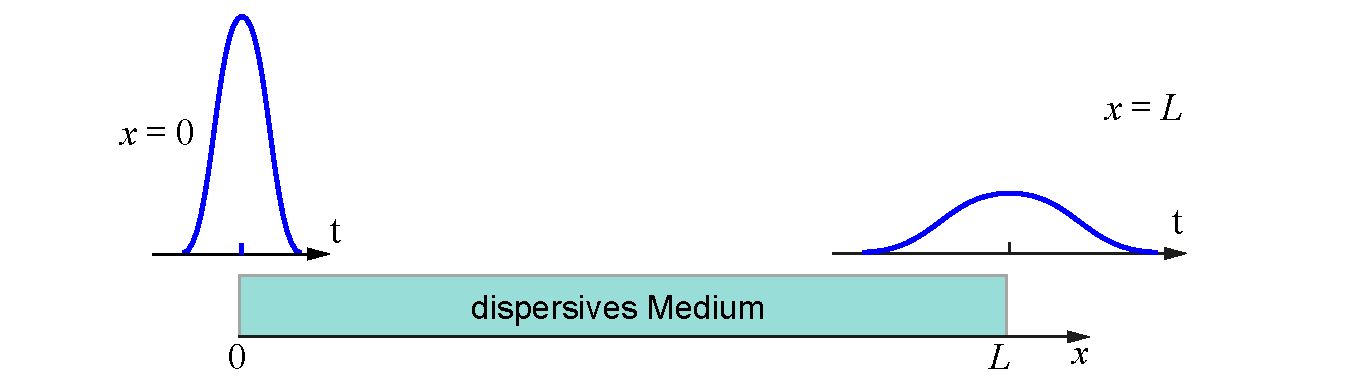
\includegraphics[width=\textwidth]{DispersionGauss.pdf}
    \caption[Wellenpaketausbreitung im dispersiven Medium.]{Auseinanderlaufen eines Gau�-f�rmigen Wellenpaketes bei Dispersion.}
    \label{abb:kontmech_DispersionGauss}
  \end{figure}

Auf Basis der Linearit�t der Wellengleichung kann man zeigen, dass sich ein solches Wellenpaket nach Durchlaufen eines dispersiven Mediums entsprechend \figref{kontmech_DispersionGauss} verbreitert und unter der verbreiterten Einh�llenden die instantane Frequenz des Wellenpaketes eine Zeitabh�ngigkeit hat, die von der Dispersion des Mediums abh�ngt. Wir werden das in der Elektrodynamik und Optik am Beispiel optischer Pulse genauer untersuchen (siehe auch \cite{Saleh2008, Schubert1986, Kaschke2014}). \\

Eine Methode der Behandlung der Ausbreitung von Wellenpaketen in dispersiven Medien besteht darin, dass man das Medium als Spektralfilter betrachtet, welches das Ausgangsspektrum des Wellenpaketes entsprechend filtert. Wir wollen das numerisch mit \matlab{} durchf�hren, indem wir zun�chst die Fourier\footnote{Jean Baptiste Joseph Fourier (1768--1830 in Paris) war ein franz�sischer Mathematiker und Physiker, der sich mit der W�rmeausbreitung in Festk�rpern besch�ftigte und dabei die Fourier-Reihen herleitete. 
Mit der nach ihm benannten Fourier-Analyse legte er einen wesentlichen Grundstein f�r moderne Physik und Technik}\indexp{Fourier, Jean Baptiste Joseph}\index{Fourier-Transformation}-Transformierte \cite{Arens2008} des Eingangswellenpaketes berechnen.\footnote{Bei diesem Aufgabenteil setzen wir Kenntnisse der Methode der Fourier-Transformation voraus. Wir werden diese ausf�hrlich in Band IV und Band V behandeln und benutzen.}

Wegen der Linearit�t der Wellengleichung k�nnen wir zeitliche Verbreiterung des Wellenpaketes und den Frequenzverlauf innerhalb des Wellenpaketes nach Durchlaufen des dispersiven Mediums als Wirkung eines linearen Filter im Frequenzraum betrachten. Wir brauchen dazu die Fourier-Transformierte des dispersiven Mediums und bilden anschlie�end das Produkt von den beiden Fourier-Transformierten. Die R�cktransformation des Produktes ergibt die zeitliche Form des Wellenpaketes nach Durchlaufen des dispersiven Mediums.\\

  \medskip
  \hyperref[lsg:kontmech_Dispersion2]{\textcolor{blue} {$\rightarrow$ L�sungsvorschlag}}.\\
  %\href{FingerUeb1_AB.pdf#lsg:kontmech_Dispersion2}{\textcolor{blue} {$\rightarrow$ L�sungsteil}}.\\
\noindent\rule[1ex]{\textwidth}{0.5pt}
\end{prob} 



% ----------------------------------------------------------------------------------------------------------

\begin{prob} %�bung26
\mittel{kontmech_soliton1}{Solitonen I}\index{Solitonen}
Solitonen sind sogenannte Einzelwellen (Englisch: \textit{Solitary Waves}), die sich formstabil �ber theoretisch unbegrenzt lange Strecken ausbreiten. Sie bewegen sich mit einer konstanten Amplitude und einem festen symmetrischen Profil. Ihre Kammlinien (das sind die Verbindungslinien zwischen den h�chsten Punkte eines Wellenzuges) sind somit Geraden. 
Solitonen wurden erstmals 1834 von dem schottischen Ingenieur Russell\footnote{John Scott Russell (1808--1882) war ein schottischer Ingenieur und Schiffbauer. Bekannt ist er durch die Entdeckung der Solitonen und die Konstruktion f�r sehr gro�er Schiffe (zumindest f�r die damalige Zeit).}\indexp{Russell, John Scott} beschrieben. Russell ritt mehrere Kilometer neben einer etwa 10 Meter langen und etwa einen halben Meter hohen Wasserwelle, die sich in einem engen Kanal ausbreitete und deren Wellenform sich kaum ver�nderte.

Solitonen entstehen durch ein Wechselspiel von Dispersion\index{Dispersion} und nichtlinearer Wechselwirkung des Ausbreitungsmedium mit der Welle. In \cite{Saleh2008} wird ein anschauliches mechanisches Analogon f�r ein Soliton gegeben (\figref{kontmech_soliton_principle}). Danach bewegt sich eine Sportwagen, ein LKW und ein Fahrrad nacheinander als Teil einer Welle. Der Sportwagen hat eine gr��ere Eigengeschwindigkeit als der LKW und dieser wiederum als der Fahrradfahrer. Auf einem festen Untergrund w�rde die Welle auseinanderlaufen, die unterschiedlichen Eigengeschwindigkeiten ergeben sich aus der Dispersion des Mediums. Ist der Untergrund elastisch (das entspricht der Nichtlinearit�t), dann sinkt der LKW ein und erzeugt eine r�cktreibende Kraft auf den Sportwagen und eine vorw�rtstreibende Kraft auf den Radfahrer. Sind Nichtlinearit�t und Dispersion gut aufeinander abgestimmt, bleiben die drei zusammen. Wir haben dann ein "`Soliton"'.\\

  \begin{figure}
    \centering
    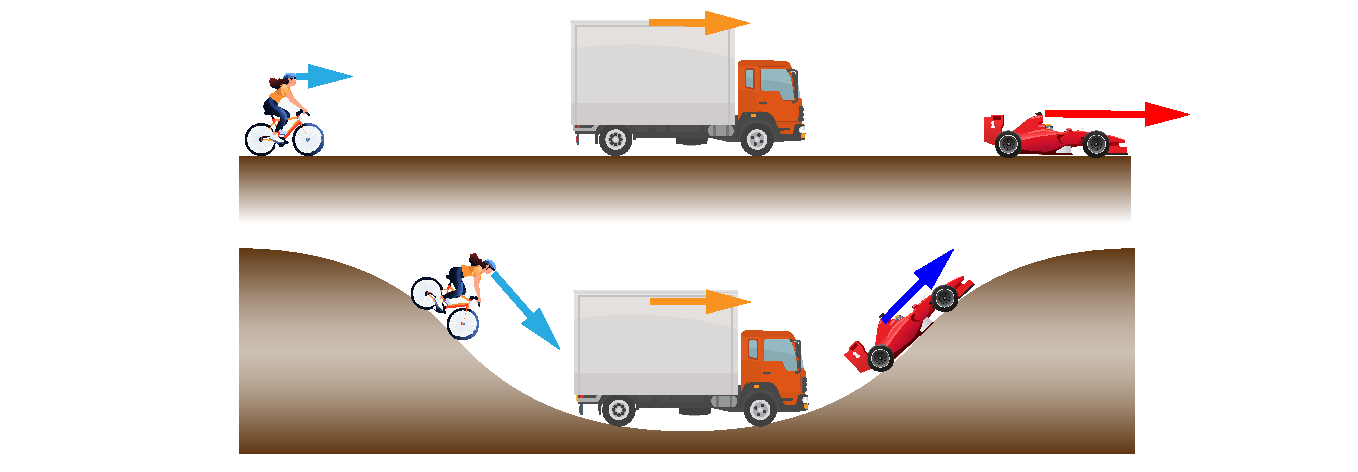
\includegraphics[width=\textwidth]{SolitonModell.pdf}
    \caption[Mechanisches Analogon eines Solitons.]{Mechanisches Analogon eines Solitons (nach \cite{Saleh2008}).}
    \label{abb:kontmech_soliton_principle}
  \end{figure}
	
Erst 1895 wurde das Ph�nomen der Solitonenwellen mathematisch-physikalisch durch die Korteweg-de-Vries-Gleichung\index{Korteweg-de-Vries-Gleichung} (KdV-Gleichung) beschrieben. Die KdV-Gleichung ist im Gegensatz zu den bisher behandelten Wellengleichungen \eqref{eq:kontmech_GrundformPDGL2} \bzw \eqref{eq:kontmech_WasswerwellenAnsatz3} eine nichtlineare Wellengleichung, da sie ja die Nichtlinearit�t des Ausbreitungsmediums beinhalten muss:
\begin{equation}
  \frac{\partial \psi}{\partial t} + 6\,\psi\,\frac{\partial \psi}{\partial x} + \frac{\partial^3 \psi}{\partial x^3} = 0\,. \label{eq:kontmech_soliton01}
\end{equation}
Hier ist $\psi$ die Wellenh�he und $x$ wurde als Ausbreitungsrichtung gew�hlt.
Man findet als L�sung f�r die KdV-Gleichung: 
\begin{align}
  \psi(x,t) = \frac{c}{2}\;\sech^2\lek \frac{\sqrt{c}}{2}\;\lk x-ct \rk \rek = \frac{c}{2}\;\lek \cosh\lk \frac{\sqrt{c}}{2}\;\lk x-ct \rk \rk \rek^{-2} \,.\label{eq:kontmech_soliton02}
\end{align}
Hier steht $c$ f�r die Ausbreitungsgeschwindigkeit in $x$\,-Richtung. Offensichtlich sind Amplitude und Ausbreitungsgeschwindigkeit nicht unabh�ngig voneinander. 
Da die KdV-Gleichung nichtlinear ist, gilt anders als f�r die Wellengleichung \eqref{eq:kontmech_WasswerwellenAnsatz3} kein Superpositionsprinzip.
\begin{enumerate}
	\item Stellen Sie die Solitonen-L�sungen \eqref{eq:kontmech_soliton02} in einer Simulation graphisch dar und beobachten Sie Form und Ausbreitung in Abh�ngigkeit vom Parameter $c$.
	\item Zeigen Sie durch Einsetzen von \eqref{eq:kontmech_soliton02} in die KdV-Gleichung \eqref{eq:kontmech_soliton01}, dass diese tats�chlich L�sungen sind.
	\item Zeigen Sie: Wenn $\psi_1$ und $\psi_2$ L�sungen der KdV-Gleichung sind, dann sind $\psi_1+\psi_2$ und $\alpha\,\psi_1$ keine L�sungen.
	\item L�sen Sie die KdV-Gleichung numerisch mit der Methode der finiten Differenzen\index{Finite Differenzen Methode}. 
	\item Solitonen bleiben nach der Interaktion mit anderen Solitonen erhalten. Berechnen Sie numerisch die dabei beobachtete Phasenverschiebung.  
\end{enumerate}

\medskip
\hyperref[lsg:kontmech_soliton1]{\textcolor{blue} {$\rightarrow$ L�sungsvorschlag}}.\\
%\href{FingerUeb1_AB.pdf#lsg:kontmech_soliton1}{\textcolor{blue} {$\rightarrow$ L�sungsteil}}.\\

\noindent\rule[1ex]{\textwidth}{0.5pt}
\end{prob}

%-----------------------------------------------------------------------------------------------------------

\begin{prob} %�bung27
\mittel{kontmech_soliton2}{Solitonen II}
Neben der Korteweg-de-Vries-Gleichung gibt es andere nichtlineare Wellengleichungen, die Solitonen als L�sungen haben. Wir m�chten zwei Gleichungen angeben:\\

\textit{\textbf{Sinus-Gordon-Gleichung (SG-Gleichung)}}\\

Die Sinus-Gordon\footnote{Walter Gordon (1893--1939) war ein deutscher Physiker, der vor allem im Bereich der mathematischen Physik und der Quantenelektrodynamik arbeitete.}\indexp{Gordon, Walter}-Gleichung\index{Sinus-Gordon-Gleichung} beschreibt unter anderem den Kontinuumsgrenzwert einer Kette harmonisch gekoppelter Pendel. Sie wird oft als N�herung f�r nichtlineare Wellenph�nomene, beispielsweise in der nichtlinearen Optik, verwendet. Der Name Sinus-Gordon-Gleichung\index{Klein-Gordon-Gleichung} ist ein Wortspiel mit Anspielung auf die �hnliche Form der Klein\footnote{Oskar Benjamin Klein (1894--1977) war ein schwedischer Physiker, der auf den Gebieten der Relativit�tstheorie und der Quantentheorie arbeitete.}\indexp{Klein, Oskar Benjamin}-Gordon-Gleichung, welche spinlose Teilchen im Rahmen der Quantenmechanik relativistisch korrekt beschreibt. Die Sinus-Gordon-Gleichung lautet:
\begin{equation}
  \frac{1}{c^2}\frac{\partial^2 \psi}{\partial t^2}  - \frac{\partial^2 \psi}{\partial x^2}  + \sin \psi = 0\,. \label{eq:kontmech_soliton03}
\end{equation}
Auch f�r die SG-Gleichung kann man geschlossene L�sungen angeben:
\begin{equation}
  \psi(x,t) = 4 \arctan \lk \mathrm{exp}\lek \pm \frac{x-vt}{\sqrt{1-(v/c)^2}}
  \rek \rk \; .
  \label{eq:kontmech_soliton04}
\end{equation}

\textbf{\textit{Nichtlineare Schr�dinger-Gleichung (NLS-Gleichung)}} \\

Die Ausbreitung von Lichtimpulsen in Wellenleitern mit nichtlinearem Brechungsindex kann mit der nichtlinearen Schr�dinger\footnote{Erwin Rudolf Josef Alexander Schr�dinger (1887--1961) war ein �sterreichischer Physiker und Wissenschaftstheoretiker. Er gilt als einer der Begr�nder der Quantenmechanik und erhielt 1933 den Nobelpreis f�r Physik.}\indexp{Schr�dinger, Erwin Rudolf Josef Alexander}-Gleichung beschrieben werden:
\begin{equation}
  \im\,\frac{\partial \psi}{\partial t} + \frac{1}{2}\,\frac{\partial^2 \psi}{\partial x^2} + g\, \left|\psi\right|^2\,\psi = 0  \,. \label{eq:kontmech_soliton05}
\end{equation}
Sie wird als Modell f�r Wasserwellen oder auch in der nichtlinearen Optik benutzt. Optische Solitonen sind von gro�er Bedeutung und Gegenstand der Forschung. Es gelang, optische Solitonen �ber mehr als $\SI{100e6}{\kilo\metre}$ ohne merkliche Verluste �ber geeignete Glasfasern zu �bertragen \cite{Saleh2008}.
Auch f�r die NLS-Gleichung kann man geschlossene L�sungen angeben. Die sogenannte Fundamentall�sung lautet:
\begin{align}
	\psi(x,t) = A_0\;\sech \lk \frac{t- x/v }{\tau_0} \rk \mathrm{exp}\lek -\im \frac{x}{x_0} \rek \,.\label{eq:kontmech_soliton06}
\end{align}
Hier sind $\tau_0$ die zeitliche Impulsl�nge, $z_0$  ist eine Gr��e f�r die lineare Dispersion (Dispersionsl�nge) und $A_0$ ist die Maximalamplitude des Solitons, die wiederum �ber $A_0\,\tau_0 = C_\text{nl,d}$ mit dem Materialparameter $C_\text{nl,d}$ verkn�pft ist, der sowohl von der Dispersion als auch der Nichtlinearit�t abh�ngt und eine Konstante ist.
Es gibt aber eine ganze Reihe von L�sungen f�r die NLS-Gleichung. So gibt es auch Solitonen h�herer Ordnung, \zb ist das Soliton 2.Ordnung gegeben durch \cite{Saleh2008}:
\begin{align}
	%\psi(x,t) = 4 \, \frac{\cosh{3t} + 3 \e^{4\im z}\, \cosh{t}}{\cosh{4t} + 4\cosh{2t} + 3\cosh{4z}} \e1{\im z/2} \,.\label{eq:kontmech_soliton07}
	\psi(x,t) = 4 \, \frac{\cosh{3t} + 3 \e^{4\im x}\, \cosh{t}}{\cosh{4t} + 4\cosh{2t} + 3\cosh{4x}} \mathrm{exp}\lek -\im \frac{x}{2} \rek \,.\label{eq:kontmech_soliton07}
\end{align}

Wir wollen die verschiedenen Solitonen-L�sungen etwas miteinander vergleichen und dabei auch auf \probref{kontmech_soliton1} zur�ck greifen.
\begin{enumerate}
	\item Stellen Sie die Solitonen-L�sungen Gl. \eqref{eq:kontmech_soliton04} und Gl. \eqref{eq:kontmech_soliton06}, als Zusatz gern auch nach Gl. \eqref{eq:kontmech_soliton07}, in einer Simulation graphisch dar und beobachten Sie Form und Ausbreitung in Abh�ngigkeit von den Parametern.
	\item Zeigen Sie durch Einsetzen in die Gleichung \eqref{eq:kontmech_soliton03} \bzw \eqref{eq:kontmech_soliton05}, dass dies tats�chlich L�sungen der jeweiligen PDGL sind.
	\item L�sen Sie die PDGL \eqref{eq:kontmech_soliton03} und \eqref{eq:kontmech_soliton05} numerisch mit der Methode der finiten Differenzen. 
	\item Vergleichen Sie die verschiedenen Solitonen-L�sungen miteinander, welche Gemeinsamkeiten, welche Unterschiede gibt es? 
\end{enumerate}

\medskip
\hyperref[lsg:kontmech_soliton2]{\textcolor{blue} {$\rightarrow$ L�sungsvorschlag}}.\\
%\href{FingerUeb1_AB.pdf#lsg:kontmech_soliton2}{\textcolor{blue} {$\rightarrow$ L�sungsteil}}.\\

\noindent\rule[1ex]{\textwidth}{0.5pt}
\end{prob}

%-----------------------------------------------------------------------------------------------------------
\newpage
\begin{prob} %�bung28
\mittel{kontmech_tsunamis}{Tsunamis}
Nach den verheerenden Folgen des Tsunamis vom Dezember 2004 im Indischen Ozean sind zahlreiche Artikel zur Mathematik von Tsunamis erschienen. Oft werden Solitonen zur mathematischen Modellierung von Tsunamis herangezogen \cite{Ziegler2005}. Obwohl Tsunamis und Solitonen �hnliche Eigenschaften aufweisen, handelt es sich doch um grunds�tzlich unterschiedliche Wasserwellenph�nomene. Es gibt sowohl Argumente f�r eine Modellierung als Soliton als auch Argumente f�r die Flachwasserwellentheorie \cite{Constantin2007}.

\begin{enumerate}
	\item Berechnen Sie den Energieeintrag in den indischen Ozean durch das Erdbeben. Bei diesem schnellte auf einer elliptischen Fl�che von 100 km Breite und 1000 km L�nge ein Teil der Burma-Platte, der von der absinkenden indischen Platte nach unten gezogen wurde, nach oben zur�ck und �bertrug so enorme Energie auf das dar�berliegende Wasser. Zus�tzlich wird vermutet, dass Unterwasser-Erdrutsche den Effekt noch verst�rkten. Insgesamt wurde sch�tzungsweise eine Energie von rund 475 Megatonnen TNT (1 MT (TNT) = \SI{4.184e15}{\joule}) freigesetzt. Sch�tzen Sie die Masse des bewegten Wassers ab und die ungef�hre H�he der Absenkung des Ozeanbodens.
	\item Argumentieren Sie entweder f�r das Tsunami- oder das Flachwasserwellen-Modell.
	\item Berechnen Sie numerisch das Aufsteilen einer Wasserwelle im K�stenbereich durch die abnehmende Wassertiefe.
\end{enumerate}

\medskip
\hyperref[lsg:kontmech_tsunamis]{\textcolor{blue} {$\rightarrow$ L�sungsvorschlag}}.\\
%\href{FingerUeb1_AB.pdf#lsg:kontmech_tsunamis}{\textcolor{blue} {$\rightarrow$ L�sungsteil}}.\\

\noindent\rule[1ex]{\textwidth}{0.5pt}
\end{prob}

%-----------------------------------------------------------------------------------------------------------
\newpage

%%%%%%%%%%%%%%%%%%%Zusatzaufgaben---------------------------------------------------------------------------

\subsection{Weiterf�hrende Zusatzaufgaben und Probleme}
\medskip

%-----------------------------------------------------------------------------------------------------------

\begin{prob} %Zusatz1
  \zusatz{kontmech_Hurrican}{Entstehung und Str�mungsprofile eines Hurrikans}
  Erkl�ren Sie die Entstehung und die Str�mungsprofile eines Hurrikans. K�nnen
  Sie eine Absch�tzung der Gr��enordnung der Terme in der
  Navier-Stokes-Gleichung machen? 
	
  \medskip  

\noindent\rule[1ex]{\textwidth}{0.5pt}
\end{prob}

%-----------------------------------------------------------------------------------------------------------
\newpage
\begin{prob} %Zusatz2
  \zusatz{kontmech_Regentropfen}{Fallgeschwindigkeit von Regentropfen}
  Berechnen Sie die maximale Fallgeschwindigkeit von Regentropfen. Ber�cksichtigen Sie dabei die unterschiedlich Form als Funktion der Gr��e.

  Phillip Lenard\footnote{Philipp Eduard Anton Lenard (1862--1947) war ein
    deutscher Physiker, der f�r seine Arbeiten �ber Kathodenstrahlen und die
    Entwicklung der Elektronentheorie 1905 den Nobelpreis f�r Physik erhielt.
    Sp�ter wurde er zum erkl�rten Gegner Einsteins und der Relativit�tstheorie
    und zum Wortf�hrer einer nationalsozialistisch-rassistisch gepr�gten
    "`Deutschen Physik"'.}\indexp{Lenard, Philipp Eduard Anton} fand
  heraus, dass gr��ere Regentropfen schneller fallen als kleine. Sind jedoch
  Regentropfen gr��er als $\SI{4.5}{\mm}$ bis $\SI{5}{\mm}$, zerfallen sie in
  zwei oder mehrere kleine. Lenard schlussfolgerte, dass Regentropfen niemals
  schneller fallen k�nnen als ca. $\SI{29}{\km\per\hour}$. Wie stehen Sie zu
  dieser Aussage? Berechnen Sie die maximale Fallgeschwindigkeit f�r Tropfen
  im Bereich von $\SI{1}{\milli\metre}$ bis $\SI{5}{\milli\metre}$ und
  ber�cksichtigen Sie dabei die Formver�nderung von einer ann�hernden
  Kugelform zu einer Form, die einem Hamburger-Br�tchen �hnelt und die wir
  durch eine Halbkugel ann�hern wollen. Die Berechnung der exakten Form eines
  Regentropfen als Funktion seiner Gr��e (und damit Masse) erfolgt unter
  Ber�cksichtigung von Oberfl�chenspannung und hydrostatischen und
  aerostatischen Druck und findet sich f�r interessierte Leser in
  \cite{Beard1987} und in einer zusammenfassenden Darstellung in
  \cite{Lim2006}.
  
  %\begin{figure}
    %\centering
    %
\includegraphics[width=\textwidth]{Platzhalter.pdf}
    %\caption[Regentropfen verschiedener Gr��e.]{Regentropfen verschiedener
      %Gr��e.}
    %\label{abb:kontmech_regentropfen}
  %\end{figure}
\medskip  

\noindent\rule[1ex]{\textwidth}{0.5pt}
\end{prob}

%------------------------------------------------------------------------------------------------------------



 
\end{PartU}

\renewcommand{\thechapter}{L\,\arabic{chapter}}

\begin{PartL}{L�sungsvorschl�ge - Band I Mechanik}
%
\begingroup
\newpage
\thispagestyle{empty}
\quad 
\endgroup
\newpage 
\setcounter{chapter}{1}
\setcounter{section}{0}
\setcounter{subsection}{0}
\setcounter{figure}{0}
\setcounter{equation}{0}
\setcounter{prob}{0}
\counterwithin{table}{section}
\setcounter{table}{0}
\begingroup
\let\cleardoublepage\relax
%%% Anmerkung 2023-05-15 (up.):
%%% Links basieren im Falle getrennter pdf-Zieldokumente auf pdf-Hypertags:
%%%        \href{PhysikUncut_Part1.pdf#prb:bew_KOS_Formel}{\textcolor{blue} {$\rightarrow$ zur \probref{bew_KOS_Formel}.}}\\
%%%
%%% oder f�r ein einziges Zieldokument auf normalen Verweisen:
%%%        \textcolor{blue} {$\rightarrow$ zur} \probref{bew_KOS_Formel}.\\
%%%
\section{L�sungsbeispiele \autoref{chap:bew} -- Physik der Bewegung von K�rpern}\label{chap:bew_lsguebungen}

Die in den L�sungsvorschl�gen angegebenen \mscre finden sich im GitHub unter \githubSN \bzw
in den \onlineZ{} (\MKc).\\
Sie sind wirklich als Vorschlag f�r eine m�gliche L�sung gedacht, wohl wissend, dass es in der Physik oft ganz verschiedene, manchmal auch elegantere als die hier vorgestellten L�sungen gibt, um ein Problem zu l�sen. Das macht ja gerade den Reiz der Physik aus.
Wir laden die Leser ein, ihre L�sungen auch unter \githubSN \bzw auf den online-Seiten (\MKc) zu teilen.
Wir sind in jedem Fall gespannt.

%%%-----------------------------------------------------------------------------------------------------------
%%%-----------------------------------------------------------------------------------------------------------

\subsection{�bungen zu Grundlagen der Mechanik von Massepunkten und Massepunktsystemen und zum Lagrange-Formalismus}

\medskip

%-----------------------------------------------------------------------------------------------------------
\hypertarget{lsg:bew_KOS_Formel}{}
\begin{sol}{prob:bew_KOS_Formel}\label{lsg:bew_KOS_Formel} %�bung1
\textbf{Differentialanalysis in Koordinatensystemen}\\ \\
Wir leiten exemplarisch die Beschleunigung in Kugelkoordinaten her.
Wir benutzen \figref{lsg_Uebung01}.
\begin{figure}
\centering
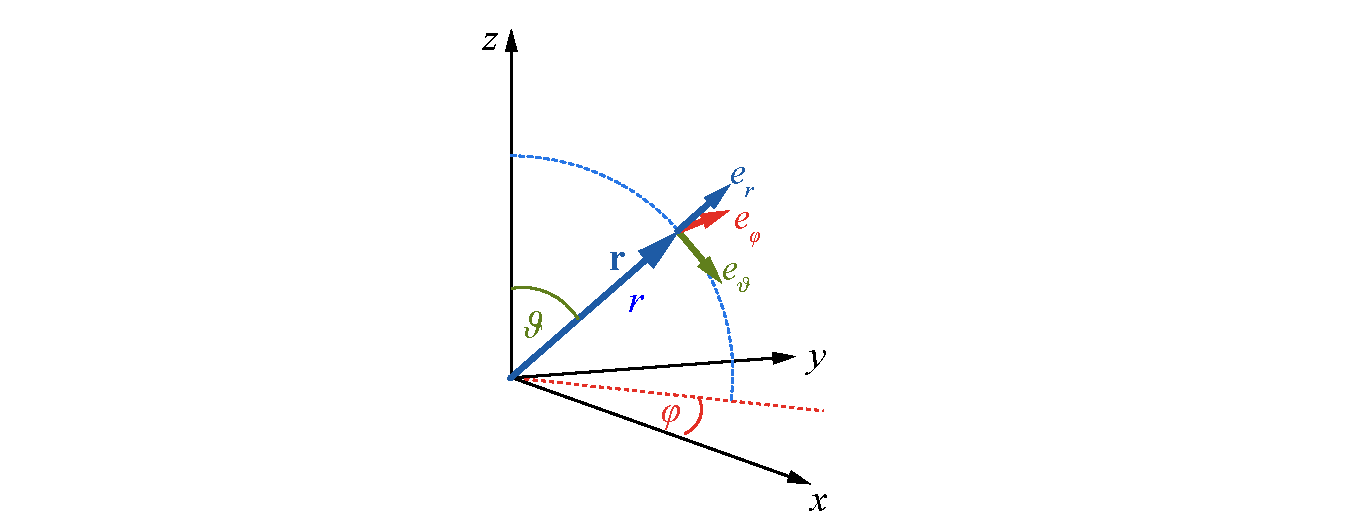
\includegraphics[width=\textwidth]{UebungKOS.pdf}%
\caption{Zur Herleitung der Beschleunigung in Kugelkoordinaten}
\label{abb:lsg_Uebung01}
\end{figure}

Die Vektoren $\vec{e}_r, \vec{e}_\vartheta, \vec{e}_\varphi$ bilden hierbei ein Rechtssystem.
Es ist $\vec{r}=r\:\vec{e}_r$ und die differentielle �nderung des Vektors kann man leicht geometrisch ableiten zu
\begin{align}
\D\vec{r} = \D r\:\vec{e}_r + r\,\D\vartheta\:\vec{e}_\vartheta + r\sin\vartheta \,\D\varphi\:\vec{e}_\varphi ~. \label{eq:lsg_bew_KOS_Formel1}
\end{align}
Daraus folgt 
\begin{align}
\vec{v} = \frac {\D\vec{r}}{\D t} = \dot{r}\:\vec{e}_r+r\dot{\vartheta}\:\vec{e}_\vartheta+r\sin\vartheta\:\dot{\varphi}\:\vec{e_\varphi} ~. \label{eq:lsg_bew_KOS_Formel2}
\end{align}
W�hrend sich $\vec{v}$ unmittelbar aus $\D\vec{r}$ ergibt, ist $\vec{a} = \dot{\vec{v}} = \ddot{\vec{r}}$ deutlich komplizierter, weil die Einheitsvektoren $\vec{e}_r, \vec{e}_\vartheta, \vec{e}_\varphi$ von $\vec{r}$ und damit von t abh�ngen.
Wir finden:
\begin{align}
\vec{a} = \dot{\vec{v}} = \ddot{r}\:\vec{e}_r + \dot{r}\:\dot{\vec{e}}_r + \dot{r}\,\dot{\vartheta}\:\vec{e}_\vartheta + r\,\ddot{\vartheta}\:\vec{e}_\vartheta + r\,\dot{\vartheta}\:\dot{\vec{e}}_\vartheta + \dot{r} \sin\vartheta\:\dot{\varphi}\:\vec{e}_\varphi \ldots \nonumber \\
+ \: r\,\dot{\vartheta}\:\cos\vartheta\:\dot{\varphi}\:\vec{e}_\varphi+ r\sin\vartheta\:\ddot{\varphi}\:\vec{e}_\varphi + r\sin\vartheta\:\dot{\varphi}\:\dot{\vec{e}}_\varphi \,. \label{eq:lsg_bew_KOS_Formel3}
\end{align}
Die zeitlichen Ableitungen der Einheitsvektoren berechnen sich nach
\begin{align*}
\dot{\vec{e}}_r &= \frac{\D}{\D t} \frac{\vec{r}}{r} = \frac{\vec{v}r-\vec{r}\dot{r}}{r^2} = \killA{\frac{\dot{r}}{r}\:\vec{e}_r} + \dot{\vartheta}\:\vec{e}_\vartheta + \sin\vartheta\:\dot{\varphi}\:\vec{e}_\varphi - \killA{\frac{\dot{r}}{r}\:\vec{e}_r} \,, \\
\dot{\vec{e}}_\varphi &= \frac{\D}{\D t} \frac{\vec{e}_z \times \vec{e}_r}{\sin\vartheta} = \frac{\vecez\times\dot{\vec{e}}_r\:\sin\vartheta - \vecez \times \vec{e}_r \:\dot{\vartheta}\,\cos\vartheta}{\sin^2\vartheta}\\
&= \frac{\vecez\times(\dot{\vartheta}\:\vec{e}_\vartheta + \sin\vartheta\;\dot{\varphi}\:\vec{e}_\varphi)}{\sin\vartheta} - \vec{e}_\varphi\frac{\dot{\vartheta}\cos\vartheta}{\sin\vartheta} = \killA{\vec{e_\varphi}\frac{\dot{\vartheta}\cos\vartheta}{\sin\vartheta}} + \dot{\varphi}\:\vecez \times \vec{e}_\varphi - \killA{\vec{e_\varphi}\frac{\dot{\vartheta}\cos\vartheta}{\sin\vartheta}} \\
&= \dot{\varphi} \lk -\sin\vartheta\:\vec{e}_r - \cos\vartheta\:\vec{e}_\vartheta \rk = - \sin\vartheta\,\dot{\varphi}\:\vec{e}_r - \cos\vartheta\,\dot{\varphi}\:\vec{e}_\vartheta ~~ \text{bzw.} \\
\dot{\vec{e}}_\vartheta &= \frac{\D}{\D t}(\vec{e}_\varphi\times\vec{e}_r) = \dot{\vec{e}}_\varphi \times \vec{e}_r + \vec{e}_\varphi \times \dot{\vec{e}}_r = -\cos\vartheta\,\dot{\varphi}\:\vec{e}_\vartheta \times \vec{e}_r + \dot{\vartheta}\:\vec{e}_\varphi \times \vec{e}_\vartheta \nonumber = \cos\vartheta\,\dot{\varphi}\:\vec{e}_\varphi - \dot{\vartheta}\:\vec{e}_r \,.
\end{align*}
Dann ergibt sich aus \eqref{eq:lsg_bew_KOS_Formel3} f�r die Beschleunigung $\vec{a}$ der etwas un�bersichtliche Ausdruck:
\begin{align}
\vec{a} &= \lk \ddot{r} - r\dot{\vartheta^2} - r\sin^2\vartheta\,\dot{\varphi^2} \rk \:\vec{e}_r + \lk \dot{r}\,\dot{\vartheta} + \dot{r}\,\dot{\vartheta} + r\,\ddot{\vartheta} - r\sin\vartheta\cos\vartheta\dot{\varphi^2} \rk \:\vec{e}_\vartheta \ldots \nonumber \\
&+ \lk \dot{r}\sin\vartheta\,\dot{\varphi} + r\,\dot{\vartheta}\,\cos\vartheta\,\dot{\varphi} + \dot{r}\,\sin\vartheta\,\dot{\varphi} + r\,\dot{\vartheta}\,\cos\vartheta\,\dot{\varphi} + r\,\sin\vartheta\,\ddot{\varphi} \rk \:\vec{e}_\varphi \nonumber \\
&= \lk \ddot{r} - r\,\dot{\vartheta^2} - r\,\sin^2\vartheta\,\dot{\varphi^2})\:\vec{e}_r + (2\dot{r}\,\dot{\vartheta} + r\,\ddot{\vartheta} - r\,\sin\vartheta\,\cos\vartheta\,\dot{\varphi^2} \rk \:\vec{e}_\vartheta \ldots \nonumber \\
&+ \lk 2\dot{r}\,\sin\vartheta\,\dot{\varphi} + 2r\,\cos\vartheta\,\dot{\vartheta}\,\dot{\varphi} + r\,\sin\vartheta\,\ddot{\varphi} \rk \:\vec{e}_\varphi \,.\label{eq:lsg_bew_KOS_Formel4}
\end{align}
Um diesen Ausdruck zu interpretieren, teilen wir die Beschleunigung in drei Komponenten auf: die Parallelbeschleunigung $\vec{a}_\text{P}$ (entlang von $\vec{r}$), die den Betrag der Geschwindigkeit erh�ht, die Zentripetalbeschleunigung $\vec{a}_\text{Z}$ und die Coriolis-Beschleunigung $\vec{a}_\text{Cor}$:
\begin{align}
\vec{a}_\text{P} &=  \ddot{r}\,\vec{e}_r + r\,\ddot{\vartheta}\,\vec{e}_\vartheta + r\,\ddot{\varphi}\,\sin\vartheta\:\vec{e}_\varphi \nonumber \\
\vec{a}_\text{Z} &=  -\lk \dot{\vartheta}^2 + \dot{\varphi^2}\,\sin^2\vartheta\rk \,\vec{e}_r - r\,\dot{\varphi^2}\,\sin\vartheta\,\cos\vartheta \,\vec{e}_\vartheta \nonumber \\
\vec{a}_\text{Cor} &=  2\,\dot{r}\,\dot{\vartheta}\:\vec{e}_\vartheta + 2 \lk r\,\sin\vartheta \:+ \:r\,\dot{\vartheta}\,\cos\vartheta \rk \dot{\varphi}\,\vec{e}_\varphi\,.\label{eq:lsg_bew_KOS_Formel5}
\end{align}
\end{sol} 

%\href{PhysikUncut_Part1.pdf#prb:bew_KOS_Formel}{\textcolor{blue} {$\rightarrow$ zur \probref{bew_KOS_Formel}.}}\\
\textcolor{blue} {$\rightarrow$ zur} \probref{bew_KOS_Formel}.\\
\noindent\rule[1ex]{\textwidth}{0.5pt}  \newpage  \clearpage

%-----------------------------------------------------------------------------------------------------------

\hypertarget{lsg:bew_konserv_Kraft}{}
\begin{sol}{prob:bew_konserv_Kraft}\label{lsg:bew_konserv_Kraft} %�bung2
\textbf{Konservatives Kraftfeld} \\ \\
Nach Voraussetzung ist $\vec{F}=\vec{F}(\vec{r})$.
\begin{subprobs}
\subprob{Beweis, dass $\vec{F}$ konservativ ist.}
Die Arbeit berechnet sich nach: 
\begin{align*}
W = -\int{}{}\vec{F}(\vec{r})\,\D r~,
\end{align*}
bzw. differentiell geschrieben: 
\begin{align}
\D W = \frac{\d W}{\d \vec{r}} \,\D \vec{r} + \underbrace{\frac{\d W}{\d \dot{\vec{r}}} \,\d \dot{\vec{r}} + \frac{\d W}{\d t} \,\d t}_{0} ~, \label{eq:lsg_bew_konserv_Kraft1}
\end{align}
da die Kraft nur von $\vec{r}$ abh�ngig ist.
Andererseits ist die differentielle Arbeit definiert durch $\delta W= -\vec{F} \:\D\vec{r} $, woraus $\D W = \delta W$ folgt und somit
\begin{align}
\vec{F} = - \frac{\d W}{\d \vec{r}} = -\gradv \cdot W ~. \label{eq:lsg_bew_konserv_Kraft3}
\end{align}
Das entspricht genau der Definition eines konservativen Kraftfeldes.\textqed \\
%
\subprob{Beweis, dass $\vec{rot}\,\vec{F}  = 0$.}
Da $\vec{F} = -\gradv \: W$, kann man schreiben: 
\begin{align*}
\rotv \vec{F}= - \rotv \times \gradv \:W \,.
\end{align*}
Unter der Voraussetzung der Vertauschbarkeit zweiter Ableitungen, also
\begin{align*}
\frac{\d^2}{\d x_i \d x_j} = \frac{\d^2}{\d x_j \d x_i}~,
\end{align*}
kann man mit Vektoralgebra leicht zeigen, dass
\begin{align*} 
\curl \vec{F} &= \lk -\frac{\d^2}{\d y\d z} + \frac{\d^2}{\d z\d y} \rk F \,\veceX  + \lk-\frac{\d^2}{\d z\d x} + \frac{\d^2}{\d x\d z} \rk F \,\veceY + \lk -\frac{\d^2}{\d x\d y} + \frac{\d^2}{\d y\d x} \rk F \,\veceZ\\
 &= 0 \,. 
\end{align*}
Daher gilt allgemein: 
\begin{align*}
\rotv \gradv U(\vec{r}) = \rotv \gradv \,U = 0 \,. \mmqed
\end{align*}
%
\newpage
\subprob{Beweis, dass $W= -\int\vec{F}\,\D\vec{r}$ nicht vom Weg abh�ngt.}
Wir betrachten zwei Wege $S_1$ und $S_2$, die die gleichen Endpunkte haben.
Aus \eqref{eq:lsg_bew_konserv_Kraft3} folgt allgemein: 
\begin{align}
W_{S_1} = -\int\limits_{S_1} \vec{F}\,\D\vec{r} = \int\limits_{S_1} \gradv U\D\vec{r} = U(\vec{r_2}) - U(\vec{r_1}) ~. \label{eq:lsg_bew_konserv_Kraft5}
\end{align}
Analog folgt:         
\begin{align}
W_{S_2} = -\int\limits_{S_2} \vec{F}\,\D\vec{r} = \int\limits_{S_2} \gradv U\D\vec{r} = U(\vec{r_2}) - U(\vec{r_1}) ~. \label{eq:lsg_bew_konserv_Kraft6}
\end{align}
In beiden F�llen h�ngt die Arbeit also nur von der Potentialdifferenz zwischen Start- und Endpunkt ab und nicht von dem dazwischen liegenden Weg. 

\subprob{Beweis, dass $\oint\limits_{S} \vec{F} \,\D\vec{r} = 0$.}
Wir schreiben f�r die geschlossene Kurve $S = S_1 - S_2$.
Dann folgt mit den Zusammenh�ngen aus der vorigen Teilaufgabe \eqref{eq:lsg_bew_konserv_Kraft5} und \eqref{eq:lsg_bew_konserv_Kraft6} sofort:
\[\oint\limits_{S} \vec{F} \, \D\vec{r} = W_{S_1} - W_{S_2} = 0~. \mmqed \]

\end{subprobs}
\end{sol} 
%\href{PhysikUncut_Part1.pdf#prb:bew_konserv_Kraft}{\textcolor{blue} {$\rightarrow$ zur \probref{bew_konserv_Kraft}.}}\\
\textcolor{blue} {$\rightarrow$ zur} \probref{bew_konserv_Kraft}.\\
\noindent\rule[1ex]{\textwidth}{0.5pt}  \newpage  \clearpage

%-----------------------------------------------------------------------------------------------------------

\hypertarget{lsg:bew_Rot_System}{}
\begin{sol}{prob:bew_Rot_System}\label{lsg:bew_Rot_System}%�bung3
\textbf{Zeitableitung in rotierenden Koordinatensystemen} \\ \\
Wir starten von den Gleichungen f�r die zeitliche Ableitung eines beliebigen Vektors $\vec{A}$ bzw. $\vec{A'}$ in seinem jeweiligen KOS, also beispielsweise
\begin{align*}
	\frac{\D \vec{A'}}{\D t} = \frac{\D A_1'}{\D t} \:\vecpeX + \frac{\D A_2'}{\D t} \:\vecpeY + \frac{\D A_3'}{\D t} \:\vecpeZ \,~.
\end{align*}
Wollen wir die zeitliche Entwicklung im Inertialsystem berechnen, m�ssen wir noch die zeitliche Ableitung der entsprechenden Einheitsvektoren ber�cksichtigen, sodass
\begin{align}
	\frac{\D \vec{A}}{\D t} = \frac{\D \vec{A'}}{\D t} + A_1' \: \dvecepx + A_2' \: \dvecepy + A_3' \: \dvecepz \,.\label{eq:lsg_bew_Rot_System1}
\end{align}
Die Basisvektoren $\vec{e}_i$ sind im Inertialsystem fest verankert und daher konstant.
Die Basisvektoren $\vec{e}'_i$ sind fest am rotierenden System und rotieren mit der Winkelgeschwindigkeit $\vec{\omega'}$ um den Ursprung des KOS $\vec{\Sigma}'$.
Die Geschwindigkeit der gestrichenen Basisvektoren ist also
\begin{align}
	\frac{\D \vec{e}'_i(t)}{\D t} = \vec{\omega'} \times \vec{e}'_i(t) \,. \label{eq:lsg_bew_Rot_System2}
\end{align}
F�r $\vec{A}$ k�nnen wir auch den zeitabh�ngigen Ortsvektor $\vec{A}(t) = \vec{r}(t) = \vec{R}(t) + \vec{r'}(t)$ einsetzen, wobei $\vec{R}(t)$ die Verschiebung des Nullpunktes der KOS darstellt.
Mit \eqref{eq:lsg_bew_Rot_System2} kann man die Zeitableitung von $\vec{A}(t)$ berechnen, indem man die rechte Seite von \eqref{eq:lsg_bew_Rot_System1} als Operator auffasst und auf $\vec{R}(t) + \vec{r'}(t)$ anwendet.
Man erh�lt dann sofort \eqref{eq:bew_Rot_System4}.
\end{sol} 
%\href{PhysikUncut_Part1.pdf#prb:bew_Rot_System}{\textcolor{blue} {$\rightarrow$ zur \probref{bew_Rot_System}.}}\\
\textcolor{blue} {$\rightarrow$ zur} \probref{bew_Rot_System}.\\
\noindent\rule[1ex]{\textwidth}{0.5pt}  \newpage  \clearpage


%-----------------------------------------------------------------------------------------------------------
\hypertarget{lsg:bew_SpaceStation}{}
\begin{sol}{prob:bew_SpaceStation}\label{lsg:bew_SpaceStation} %�bung4
\textbf{Moderne Raumstation} \\ \\
Wir wollen annehmen, dass der Astronaut, wenn er im �u�eren Ring arbeitet, die gewohnte Erdbeschleunigung sp�rt, d.h. die Station rotiert mit:
	\begin{align*}
		\omega = \sqrt{\frac{g}{R_\text{S}}}=\sqrt{\frac{2g}{D_\text{S}}}\approx \SI{0.512}{\per\second} \,.
	\end{align*}
Das entspricht einer Umdrehungszeit von $12\,\mathrm{s}$. 
Wir wollen nun die verschiedenen Fragen zu den wirkenden Kr�ften beantworten.
\begin{subprobs}
\subprob{Bewegung entlang des Tubus}
Wir betrachten die Bewegung des Astronauten entlang des Tubus, also im Inertialsystem $\vec{\Sigma}$.
F�r die $\pi R_\text{S}\approx \SI{120}{m}$ wollen wir etwa eine Minute veranschlagen, was einer Geschwindigkeit von $v_\text{A}=\SI{2}{\meter\per\second}$ entspricht. \\
Durch die Bewegung des Astronauten �ndert sich die effektive \anf{Schwerebeschleunigung} auf den Astronauten und zwar je nachdem, in welche Richtung er relativ zur Rotationsrichtung auf die andere Seite gelangen will:
	\begin{align*}
		\text{gleichsinnige Bewegung:} \quad \omega_\text{eff}&=\omega+\frac{v_\text{A}}{R_\text{S}} \quad \Rightarrow \quad g_\text{eff,s}=\omega_\text{eff}^2\, R_\text{S} \approx \SI{12}{\meter\per\second^2} \,, \\
		\text{gegensinnige Bewegung:} \quad \omega_\text{eff}&=\omega-\frac{v_\text{A}}{R_\text{S}} \quad \Rightarrow \quad g_\text{eff,s} \approx \SI{7.9}{\meter\per\second^2}\,.
	\end{align*}
Er sollte sich also besser \anf{gegensinnig} auf die andere Seite der Station begeben.
Bei einer sich gegen den Uhrzeigersinn drehenden Station sollte er also im Uhrzeigersinn laufen.
\subprob{Bewegung entlang des senkrechten Mittelgangs}
Nun will der Astronaut eine Abk�rzung durch den direkten Verl�ngerungsgang w�hlen.
Wir betrachten seine Bewegung jetzt folglich im mitbewegten System $\vec{\Sigma}'$.
Wir betrachten zun�chst die Coriolis-Kraft.
Der Astronaut ($\SI{100}{\kg}$) wird mit dieser gegen die seitliche Wand des Tunnels gedr�ckt.
		\begin{align*}
				\vec{F}_\text{Cor}'= -2m\,\omega \begin{pmatrix}
  0\\ 
  v_\text{A} \\
	0
\end{pmatrix} \approx -200 \,\mathrm{N} \cdot \veceY \,.
		\end{align*}
Wir betrachten noch den Energieaufwand, den der Astronaut in diesen Fall gegen das k�nstliche \anf{Schwerefeld} aufbringen muss.
Beim Gang bis zur Mitte arbeitet er gegen das k�nstliche Schwerefeld, danach k�nnte er die potentielle Energie mit Hilfsmitteln wieder zur�ckgewinnen:
	\begin{align*}
		\Delta E &= \int\limits_{R_\text{S}}^{0} F_\text{z}'\,\D r' = -m\,\omega^2\,r' \,\D r' \,.\\
		&= +\frac{m}{2} \,\omega^2\,{R_\text{S}}^2 \approx \SI{18200}{\newton\meter} \approx 0.005 \,\mathrm{kWh}  \approx 4350 \, \mathrm{cal} \,.
	\end{align*}
Das ist also kein �quivalentes Training f�r den Astronauten, um fit zu bleiben.

\newpage
\subprob{Weitere Schwierigkeit}
Zum Schluss wollen wir noch die Gezeitenkraft, die wir im Detail in der Himmelsmechanik (Kapitel 3 im Teil 2 dieser Reihe) behandeln werden, absch�tzen.
Auf den Astronauten (Gr��e $\SI{2}{\meter}$) wirken ja im k�nstlichen \anf{Schwerefeld} auf seinen Kopf (K) und seine F��e (F) unterschiedlich gro�e Kr�fte.
		\begin{align*}
				F_\text{K} &= m \,g_\text{K} = m \,\omega^2 \,(R_\text{S}-h_\text{A}) \,,\\
				F_\text{F} &= m \,g_\text{F} = m \,\omega^2 \, R_\text{S}\,, \\
				\Delta F &= -m \,\omega^2 h_\text{A} \approx 52 \, \mathrm{N} \,.
		\end{align*}
Das ist ein nicht unerheblicher Kraftunterschied, dessen Wirkung auf den K�rper (Blutfluss, Koordination) sicher nicht zu vernachl�ssigen ist.
Ob sich ein Astronaut auf so einer Station wohlf�hlt bleibt abzuwarten.
Die Bedingungen kann man nat�rlich verbessern, wenn man $R_\text{S}$ gr��er macht.
\end{subprobs}
\end{sol} 
%\href{PhysikUncut_Part1.pdf#prb:bew_SpaceStation}{\textcolor{blue} {$\rightarrow$ zur \probref{bew_SpaceStation}.}}\\
\textcolor{blue} {$\rightarrow$ zur} \probref{bew_SpaceStation}.\\
\noindent\rule[1ex]{\textwidth}{0.5pt}  \newpage  



%-----------------------------------------------------------------------------------------------------------
\hypertarget{lsg:bew_SpaceElevator}{}
\begin{sol}{prob:bew_SpaceElevator}\label{lsg:bew_SpaceElevator} %�bung5
\textbf{Weltraumfahrstuhl}
\begin{subprobs}
	\subprob{Anforderungen an das Seil}  
		Wir betrachten zun�chst einen Satelliten in einer geostation�ren Umlaufbahn, dessen H�he $h_\text{G}$ �ber dem �quator man leicht ausrechnen kann, indem man im mitbewegten System $\vec{\Sigma}'$ fordert, dass die Zentrifugalkraft gleich der Gravitationskraft ist:
		\[ -\frac{G\,m_\text{E}\,m}{R_\text{G}^2} + m\,\omega_\text{E}'^2\,R_\text{G} = 0 \,, ~  R_\text{G} = R_\text{E} + h_\text{G}\, .
		\]
		Hierin sind $R_\text{E}$, $m_\text{E}$ der Radius bzw. die Masse der Erde und $\omega_\text{E}'= {2\pi}/{86125}\,\text{s}^{-1}$ die Rotationsfrequenz der Erde.
		Man erh�lt daraus eine Beziehung f�r $R_G$. Der Einfachheit halber lassen wir die Striche weg, da wir nur im mitbewegten System rechnen:
		\begin{align}
		R_\text{G} = R_\text{E} + h_\text{G} = \sqrt[3]{\frac{G\,m_\text{E}}{\omega_\text{E}^2}} \approx \SI{42000}{km} \, .
		\label{lsg:bew_SpaceElevator_1}
		\end{align}
		
\begin{figure}[H]
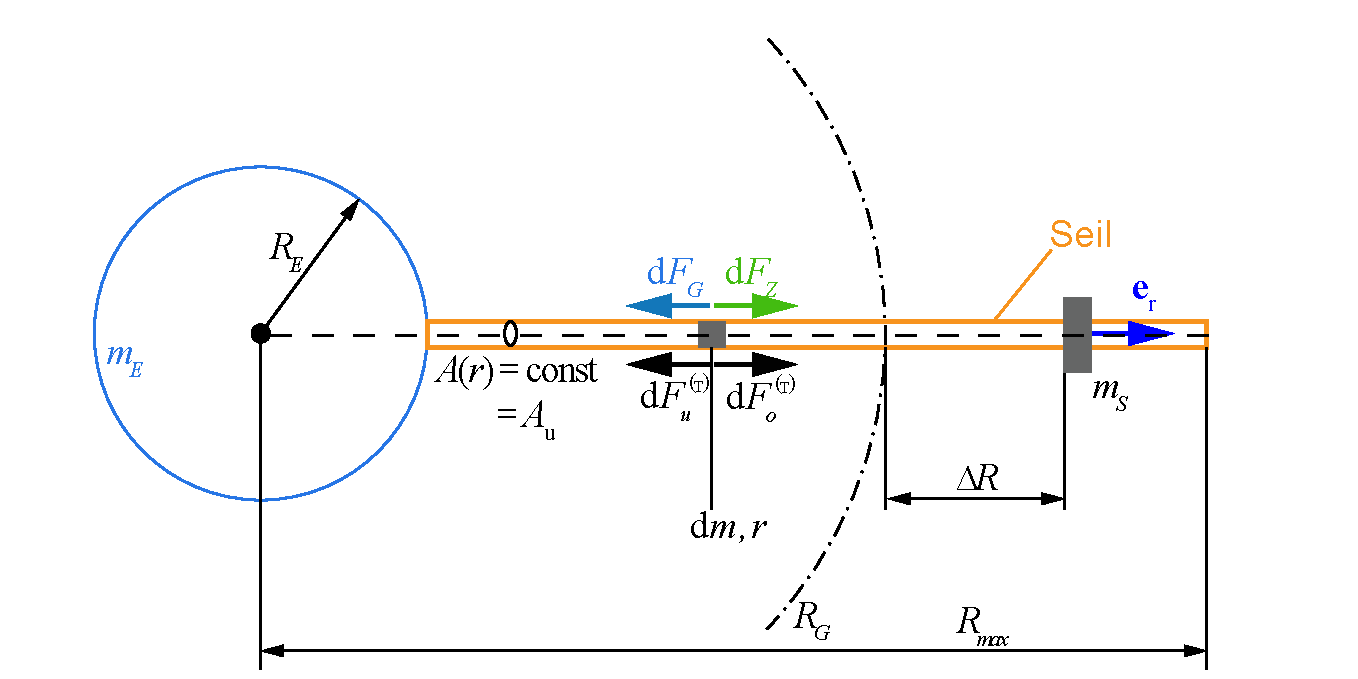
\includegraphics[width=\textwidth]{SpaceElevator_1.pdf}%
\caption{Modell des Weltraumfahrstuhls mit konstanter Seildicke}
\label{abb:lsg_SpaceElevator_1}
\end{figure}
		
	\begin{enumerate} [a) ]
		\item Konstante Seildicke \\
		Wir betrachten nun die \figref{lsg_SpaceElevator_1}.
    Das Seil muss offensichtlich im System $\vec{\Sigma} '$ ruhen. 
		F�r einen beliebigen Massepunkt entlang des Seils gilt dann nach der Zeichnung f�r den Fall eines Seils mit  konstanter Dicke und der Massendichte~$\rho$ und zun�chst einer Endmasse $m_\text{S}=0$ folgende Kr�ftebilanz, wobei die $F_\text{o,u}^{(\text{T})}$ die Seilspannungskr�fte nach oben und unten sind und $\text{d}F_\text{G}$, $\text{d}F_\text{Z}$ die differentielle Schwerkraft bzw. Zentrifugalkraft:
		\begin{align}
		F_\text{o}^{(\text{T})} - F_\text{u}^{(\text{T})} = \D F^{(\text{T})} = A_\text{u}\,\D \sigma^{(\text{T})} = A_\text{u} \,\rho \,\D r \lek  \underbrace{\frac{G \,m_\text{E}}{r^2}}_{\text{d}F_\text{G}} - \underbrace{\omega_\text{E}^2 \,r }_{\D F_\text{Z}}\rek\, .
		\label{lsg:bew_SpaceElevator_2}
		\end{align}
		Die Gr��e $\D \sigma^{(\text{T})}$ ist die differentielle Seilspannung (in \SI{}{\newton\per\meter\squared}) und hat die $r$-Abh�ngigkeit
		\begin{align}
		\frac{\D \sigma^{(\text{T})}(r)}{\D r} = G\, m_\text{E} \,\rho \,\biggl[\frac{1}{r^2} - \frac{r}{R_\text{G}^3}\biggl]\,,
		\label{lsg:bew_SpaceElevator_3}
		\end{align}
		wobei wir \eqref{lsg:bew_SpaceElevator_1} benutzt haben.
		Die Integration von $R_\text{E}$ bis $R_\text{G}$ ergibt die Spannung im Seil bei $r = R_\text{G}$:
		\begin{align}
		\sigma(R_\text{G}) = G \,m_\text{E}\,\rho\:\biggl[ \frac{1}{R_\text{E}} - \frac{3}{2R_\text{G}} + \frac{R_\text{E}^2}{2R_\text{G}^3}\biggl] \, .
		\label{lsg:bew_SpaceElevator_4}
		\end{align}
		Wir wollen nun die notwendige Seill�nge $L_\text{Seil}^{(1)}  = R_ \text{max} - R_\text{E}$ ermitteln. 
		Da das Seil im mitbewegten System ruhen muss, muss f�r alle Massepunkte die resultierende Spannung verschwinden, also mit \eqref{lsg:bew_SpaceElevator_2}:
		\begin{align}
		A_\text{u} \rho  \int_{R_\text{E}}^{R_\text{max}} r \text{d}r \,\biggl[\frac{Gm_\text{E}}{r^3} - \omega_\text{E}^2\biggl] &\overset{!}{=} 0
		\label{lsg:bew_SpaceElevator_5}\\
		\Rightarrow \frac{1}{2} \omega_\text{E}^2\,(R_\text{max}^2 - R_\text{E}^2) &= Gm_\text{E} \,\biggl(\frac{1}{R_\text{E}} - \frac{1}{R_\text{max}} \biggl)\, ,
		\end{align}
		woraus eine quadratische Gleichung f�r $R_ \text{max}$ resultiert\footnote{Eigentlich resultiert eine kubische Gleichung, aber die triviale L�sung $R_\text{max} = R_\text{E}$ kann eliminiert werden.}, deren physikalisch sinnvolle L�sung
		\begin{align}
		R_\text{max} &= \frac{R_\text{E}}{2} \lk\sqrt{1 + \frac{8 G\,m_\text{E}}{\omega_\text{E}^2 \,R_\text{E}^3} } - 1\rk = \frac{R_\text{E}}{2} \lk \sqrt{1 + 8 \lk \frac{R_\text{G}}{R_\text{E}} \rk^3} - 1\rk \:\approx \SI{150000}{km}\, , \nonumber \\
		L_\text{Seil}^{(1)} &= R_\text{max} - R_\text{E} = \frac{R_\text{E}}{2} \,\lk \sqrt{1 + 8 \lk \frac{R_\text{G}}{R_\text{E}} \rk^3} - 3\rk \:\approx \SI{144000}{km}
		\label{lsg:bew_SpaceElevator_6}
		\end{align}
		ist, wobei wir \eqref{lsg:bew_SpaceElevator_1} benutzt haben.

		\item Variabler Querschnitt mit konstanter Seilinnenspannung \\
		 Betrachten wir nun ein Seil, welches einen variablen Durchmesser hat (\figref{lsg_SpaceElevator_2}) und zwar so, dass die Spannung $\sigma_\text{c}$ im Seil �berall gleich gro� ist. 

\begin{figure}[H]
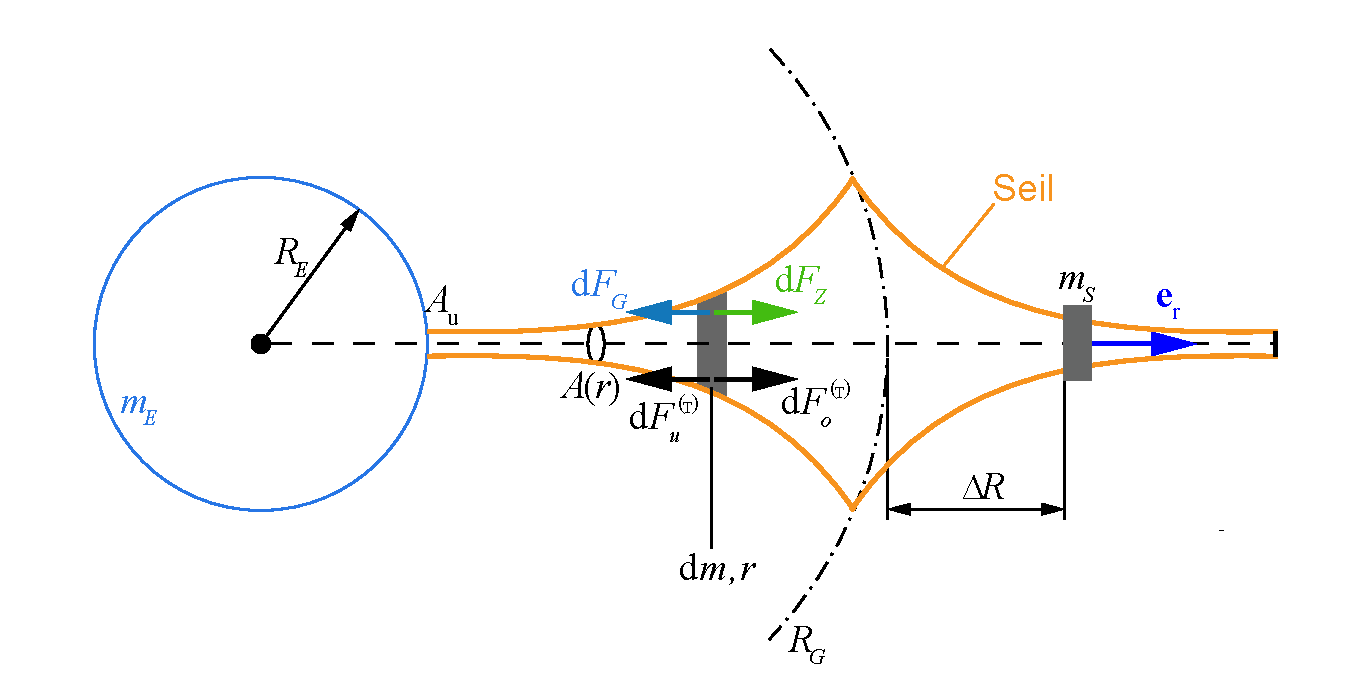
\includegraphics[width=\textwidth]{SpaceElevator_2.pdf}%
\caption[Modell des Weltraumfahrstuhls mit konstanter Seilspannung]{Modell des Weltraumfahrstuhls mit konstanter Seilspannung $\sigma_\text{c}$}
\label{abb:lsg_SpaceElevator_2}
\end{figure}

		Dann muss die Gleichung \eqref{lsg:bew_SpaceElevator_2} lauten:
		\begin{align}
		\D F_\text{o}^{(\text{T})} - \D F_\text{u}^{(\text{T})} = \sigma_\text{c} \, \D A = \rho A(r) \, \lek \frac{G \, m_\text{E}}{r^2} - \omega_\text{E}^2 \, r \rek \, \D r\, , 
		\label{lsg:bew_SpaceElevator_7}
		\end{align}
		bzw. integriert:
		\begin{align}
		A(r) = A_\text{u} \exp \lk \frac{\rho \,g \,R_\text{E}^2}{\sigma_\text{c}} \lek \frac{1}{R_\text{E}} + \frac{R_\text{E}^2}{2R_\text{G}^3} - \frac{1}{r} - \frac{r^2}{2R_\text{G}^3} \rek \rk \, .
		\label{lsg:bew_SpaceElevator_8}
		\end{align}
		Hierbei haben wir $g=\frac{G\,m_\text{E}}{R_\text{E}^2}$ gesetzt und $A(R_\text{E}) = A_\text{u}$.\\
		Die L�nge des Seils, wiederum ohne Gegengewicht ($m_\text{s}=0$), erhalten wir, indem wir fordern, dass $A(R_\text{max}) = A(R_\text{E})$:
		\begin{align}
		\Rightarrow L_\text{Seil}^{(2)} = \frac{R_\text{E}}{2} \lek \sqrt{1 + 8\lk\frac{R_\text{G}}{R_\text{E}}\rk^3} -1 \rek - \frac{2R_\text{E}}{2} = \frac{R_\text{E}}{2}\lek \sqrt{1 + 8\lk\frac{R_\text{G}}{R_\text{E}}\rk^3} -3 \rek \, ,
		\label{lsg:bew_SpaceElevator_9}
		\end{align}
		was identisch mit \eqref{lsg:bew_SpaceElevator_6} ist.
	\end{enumerate}

	\subprob{Vergleich und Argumentation zur Machbarkeit} 
	Wir wollen nun die beiden Varianten vergleichen und benutzen dazu Materialparameter von m�glichen Materialien. 
	Im Fall a) mit konstanter Seildicke m�ssen wir uns also offensichtliche Gedanken �ber die  maximal auftretende (Zug-)Spannung im Seil $\sigma_\text{max} = \sigma(R_\text{G})$ machen. 
	Bei Fall b) mit konstanter (max. zul�ssiger) Zugspannung $\sigma$ hingegen sollte eher die maximale Seildicke bzw. den Seilquerschnitt $A_\text{max} = A(R_\text{G}) = \frac{\pi}{4}d_\text{max}^2$ in Betracht gezogen werden.\\
	% (d_u = \SI{5}{\milli\meter}) % was ist das? wozu diese Angabe?
	\begin{table}[h!]
		\centering
		\caption[Berechnungen f�r Weltraumfahrstuhl auf der Erde.]{Berechnungen f�r Weltraumfahrstuhl auf der Erde f�r Fall a (Seil mit $A=\text{const}$) und Fall b (Seil mit $\sigma=\text{const}$) und verschiedene Materialien. (Mit Taper Ratio wird das Verh�ltnis von Maximal- zu Minimalseilquerschnitt bezeichnet.)}
		\begin{tabular}{lccccc}
			Material& Zugfestigkeit	& Dichte & Fall a	& Fall b &Taper Ratio\\
			&$\quad \sigma_\text{mat} \left[\SI{}{GPa}=\SI{}{\newton\per\meter\squared}\right]\quad $ & $\quad \rho \left[\frac{\text{kg}}{\text{m}^3}\right]\quad $ &$\quad \sigma_\text{max} \left[\SI{}{GPa}\right]\quad $			& $\quad d_\text{max} \left[\SI{}{\milli\meter}\right]\quad $&\\
			\midrule
			Karbon	& $\approx 100$ & $1300$ &  63	& $7 $& 1.9\\
			Kevlar	& $\approx 4 $ & $1440$ &  70	&	$3\, 10^{02}$& 3100	\\
			Dyneema	& $\approx 3 $ & $ 970$ &  44	&	$7\, 10^{01}$& 720	\\
			Stahl 	& $\approx 5 $ & $7900$ & 383	&	$2\, 10^{13}$& $2\, 10^{16}$	\\
		\end{tabular}
	\end{table}

	Man erkennt, dass es, wenn es �berhaupt eine machbare L�sung geben kann, diese nur mit Karbonfasern realisierbar w�re.
        In diesem Fall w�rde das Seil im g�nstigsten Fall $\SI{7}{\mm}$ dick sein.
	Insgesamt scheint die Realisierungschance beim Seil mit variablem Querschnitt gr��er.
        Aber selbst dann gibt es offene Fragen:
	\begin{itemize}
		\item Haltbarkeit
		\item Rei�en durch Einfluss von \anf{Space Debris} (Raumfahrtm�ll)
		\item Materialerm�dung �ber die Zeit u.v.a.m.
		\item Coriolis-Kraft: Wir haben bisher noch nicht ber�cksichtigt, dass sich eine Nutzlast mit einer bestimmten Geschwindigkeit entlang des Seils nach oben bewegen muss.
                  Wie wir im Kapitel \ref{kap:bew_Coriolis-Kraft} gesehen haben, f�hrt eine Bewegung senkrecht nach oben im rotierenden Bezugssystem zu einer seitlichen Ablenkung.
                  Das Seil w�rde also anfangen seitw�rts zu schwingen.
                  Der Leser kann mit Gleichung \eqref{eq:bew_Coriolis_Kraft} selbst absch�tzen, wie gro� die Kraft ist bzw. wie langsam sich der Fahrstuhl bewegen m�sste, damit die seitliche Kraft klein gegen�ber der Querspannung im Material bleibt.
	\end{itemize}
\subprob{Vorteile durch Anbringen eines Gegengewichts}
	Wir wollen nun noch untersuchen, ob sich die Rahmenbedingungen verbessern lassen, wenn man an geeigneter Stelle im Abstand $\Delta R$ von $R_\text{G}$ ein Gegengewicht der Masse $m_\text{c}$ anbringt.
        Dann muss dort folgende Kr�ftebilanz erf�llt sein:
	\begin{align}
	F_\text{G}^{(m_\text{S})} + F^{(\text{T})} &= F_\text{z}^{(m_\text{S})} \, ,\\
	\frac{G\, m_\text{E}\, m_\text{S}}{\left[R_\text{G}+\Delta R\right]^2} + A(R_\text{G} + \Delta R)\, \sigma &= m_\text{S}\, \omega_\text{E}^2\,\left[ R_\text{G}+\Delta R \right] \, .
	\label{lsg:bew_SpaceElevator_10}
	\end{align}
	Wir nutzen die Beziehung \eqref{lsg:bew_SpaceElevator_8} f�r $A(R_\text{G}+\Delta R)$ und erhalten f�r die Masse $m_\text{S}$ als Funktion der Position $\Delta R$:
	\begin{align}
	m_\text{S}(\Delta R) &= \frac{A_\text{u} \, \sigma_\text{mat}}{g} \frac{\mathrm{e} \lek[\frac{R_\text{E}^2\, \rho \, g}{2\sigma \, R_\text{G}^3} \lk\frac{2R_\text{G}^3 + R_\text{E}^3}{R_\text{E}} - \frac{2R_\text{G}^3 + (R_\text{G}+\Delta R)^3}{R_\text{G} + \Delta R}\rk\rek}{\frac{R_\text{E}^2\, (R_\text{G} + \Delta R)}{R_\text{G}^3}\lek 1 - \lk\frac{R_\text{G}}{R_\text{G} + \Delta R}\rk^3\rek} \,. 	\label{lsg:bew_SpaceElevator_11}
	\end{align}
	Man kann leicht sehen, dass $m_\text{S} \rightarrow \infty$, wenn $\Delta R \rightarrow 0$, also muss die Masse au�erhalb der geostation�ren Bahn liegen.
        Man kann also die L�nge des Seils ver�ndern, wenn man die Zusatzmasse $m_\text{S}$ anbringt.
        Die Gesamtmasse ist dann 
	\begin{align}
	m_\text{tot}(\Delta R) &= m_\text{S} + m_\text{Seil} = m_\text{S} + \rho \int\limits_{R_\text{E}}^{R_\text{G} + \Delta R} A(r) \, \D r \, .
	\label{lsg:bew_SpaceElevator_12}
	\end{align}
	Das Integral in Gleichung \eqref{lsg:bew_SpaceElevator_12} berechnen wir numerisch.
        In \figref{lsg_SpaceElevator_3} sind f�r die unterschiedlichen Materialparameter die Massen $m_\text{S}, ~ m_\text{Seil}$ als Funktion der Position $\Delta R$ gezeigt.
\begin{figure}[H]
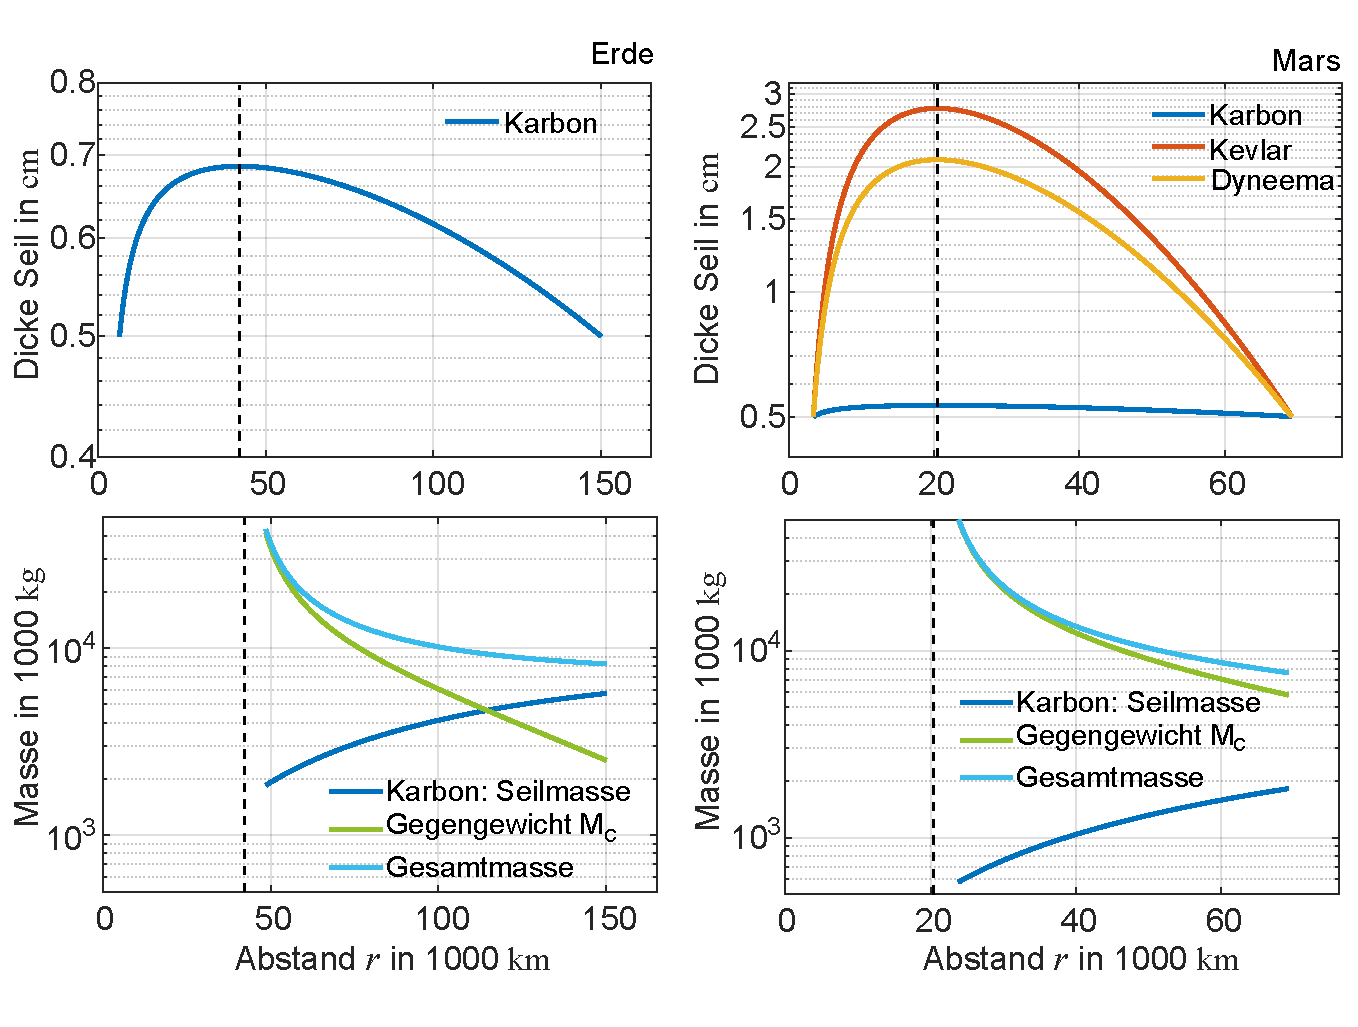
\includegraphics[width=\textwidth]{SpaceElevator_3.pdf}%
\caption[Seilmassen und Zusatzmasse]{Seilmassen und Zusatzmasse als Funktion der Position der Zusatzmasse f�r verschiedene Materialparameter}
\label{abb:lsg_SpaceElevator_3}
\end{figure}

\subprob{(Energetischer) Nutzen des Space Elevators} 
	Wir wollen nun die Energie berechnen, die mit dem Space Elevator gespart werden kann, wenn man eine Nutzmasse $m_\text{N}$ auf eine bestimmte Bahnh�he $H_\text{B} = r_\text{B} - R_\text{E}$ zu bringen hat.
	Beim Fahrstuhl muss man nur die potentielle Energie aufbringen:
	\[ W^{(1)} = \Delta E_\text{pot} = \int\limits_{R_\text{E}}^{H_\text{B}} \frac{G\,m_\text{N} m_\text{E}}{r^2} \D r = -\frac{G m_\text{N} m_\text{E}}{r}\bigg|_{R_\text{E}}^{H_\text{B}+R_\text{E}}\, .
	\]
	Bei einem Raketenstart ist die aufgewendete Arbeit, um eine Nutzlast auf $H_\text{G} = R_\text{G} - R_\text{E}$ zu bringen:
	\begin{align*}
	W^{(2)} &= \Delta E_\text{kin} + \Delta E_\text{pot} = \frac{m_\text{N}}{2}\,  \omega_\text{E}^2 \, R_\text{G}^2 + \Delta E_\text{pot}\,,
\end{align*}
woraus
	\begin{align}
\frac{\Delta W}{W^{(2)}} &= \frac{W^{(1)} - W^{(2)}}{W^{(2)}} = \frac{W^{(1)}}{W^{(2)}} - 1 \approx 8 \% 
	\end{align}
folgt. Wir haben hier nur die Arbeit f�r die Nutzlasten vergleichen.
        Beim Raketenstart m�sste man ja korrekterweise noch den Aufwand, der f�r den Transport des Treibstoffs notwendig ist, ber�cksichtigen (siehe Kapitel 4, Band II).
\subprob{Space Elevator zum Mars}
	F�r den Mars k�nnen wir die Gleichung verwenden und ersetzen
	\begin{align*}
	R_\text{E} &\rightarrow R_\text{M} = \SI{3791}{km} \, , \\
	m_\text{E} &\rightarrow m_\text{M} = \SI{6.417e23}{kg}\, ,\\
	\omega_\text{E} &\rightarrow \omega_\text{M} = \frac{2 \pi}{ 88620 \,\text{s}} = \SI{7.09e-5}{per\second} \,.
	\end{align*}
	Damit ergeben sich mit den gleichen Materialien f�r die Erde folgende Bedingungen f�r einen Weltraumfahrstuhl auf dem Mars.
        Die Realisierungsbedingungen f�r einen solchen Fahrstuhl auf dem Mars sind auf Grund dessen geringerer Masse also deutlich besser, abgesehen nat�rlich von dem logistischen Aufwand.
        Wir �berlassen dem Leser die Absch�tzung f�r den Mond (Man beachte dabei die notwendige L�nge des Seils.) und auch Investitionsentscheidung!
        F�r weitergehende Berechnungen empfehlen wir \cite{Aravind2007, Pearson2005}.\\
	% (d_u = \SI{5}{\milli\meter})
	\begin{table}[H]
		\centering
		\caption[Berechnungen f�r Weltraumfahrstuhl auf dem Mars.]{Berechnungen f�r Weltraumfahrstuhl auf dem Mars f�r Fall a (Seil mit $A=\text{const}$) und Fall b (Seil mit $\sigma=\text{const}$) und verschiedene Materialien.}
		\begin{tabular}{lccccc}
			% \toprule
			Material& Zugfestigkeit	& Dichte 	& Fall a	& Fall b\\
			&$ \quad \sigma_\text{mat} \left[\SI{}{GPa}=\SI{}{\newton\per\meter\squared}\right] \quad $
			& $ \quad \rho \left[\frac{\text{kg}}{\text{m}^3}\right] \quad $ 
			&$ \quad \sigma_\text{max} \left[\SI{}{GPa}\right] \quad $			
			& $ \quad d_\text{max} \left[\SI{}{\centi\meter}\right]  \quad $
			&Taper Ratio\\
			\midrule
			Karbon	& $\approx 100$ & $1300$ & 12	& $0.5$&1\\
			Kevlar	& $\approx 4 $  & $1440$ & 14 &	$2.8$&37	\\
			Dyneema	& $\approx 3 $  & $ 970$ & 9 &	$2.1$&21	\\
			Stahl 	& $\approx 5 $  & $7900$ & 75	&	$920$&$3.4\cdot10^6$\\
			% \bottomrule
		\end{tabular}
	\end{table}
\end{subprobs}
\end{sol} 
%\href{PhysikUncut_Part1.pdf#prb:bew_SpaceElevator}{\textcolor{blue} {$\rightarrow$ zur \probref{bew_SpaceElevator}.}}\\
\textcolor{blue} {$\rightarrow$ zur} \probref{bew_SpaceElevator}.\\
\noindent\rule[1ex]{\textwidth}{0.5pt}  \newpage


%-----------------------------------------------------------------------------------------------------------
\hypertarget{lsg:bew_SkyDiver}{}
\begin{sol}{prob:bew_SkyDiver}\label{lsg:bew_SkyDiver} %�bung6
\textbf{Skydiver} \\ \\

Die numerische Berechnung findet sich in \mlbewref{Skydiver.m}.

\end{sol} 
%\href{PhysikUncut_Part1.pdf#prb:bew_SkyDiver}{\textcolor{blue} {$\rightarrow$ zur \probref{bew_SkyDiver}.}}\\
\textcolor{blue} {$\rightarrow$ zur} \probref{bew_SkyDiver}.\\
\noindent\rule[1ex]{\textwidth}{0.5pt}  \newpage

%-----------------------------------------------------------------------------------------------------------
\hypertarget{lsg:bew_Quizfrage}{}
\begin{sol}{prob:bew_Quizfrage}\label{lsg:bew_Quizfrage} %�bung7
\textbf{Quizfrage} \\ \\

Die numerische Berechnung findet sich in \mlbewref{WurfmitohneReibung.m}.\\
Als Ergebnis ergibt sich: Im Falle mit Reibung ist die Kanonenkugel immer schneller wieder unten. Eng verwandt damit ist die folgende Frage: Braucht in einem Medium mit Reibung die Kugel im Aufstieg oder im Abstieg mehr Zeit, oder sind die Zeiten gleich lang wie im Fall ohne Reibung? Man kann das sich auch ohne numerische Rechnung leicht �berlegen.\\

(�bung nach einer Anregung durch Ref. \cite{Mungan2021}. 

\end{sol} 
%\href{PhysikUncut_Part1.pdf#prb:bew_Quizfrage}{\textcolor{blue} {$\rightarrow$ zur \probref{bew_Quizfrage}.}}\\
\textcolor{blue} {$\rightarrow$ zur} \probref{bew_Quizfrage}.\\
\noindent\rule[1ex]{\textwidth}{0.5pt}  \newpage

%-----------------------------------------------------------------------------------------------------------
\hypertarget{lsg:bew_VielteilchenI}{}
\begin{sol}{prob:bew_VielteilchenI}\label{lsg:bew_VielteilchenI}%�bung8
\textbf{Vielteilchensysteme} \\ \\
Wir wollen die G�ltigkeit folgender Erhaltungss�tze f�r Vielteilchensysteme zeigen.
\begin{subprobs}
\subprob{Impulserhaltung}
Aus \eqref{eq:bew_Gesamtgroessen} folgt mit 
$M = \sum\limits_{i} m_i$ und $\vec{R}= \frac{1}{M} \sum\limits_{i} m_i \, \vec{r}_i$, dass 
\begin{align*}
	&\sum\limits_{i} m_i \, \ddot{\vec{r}}_i = M  \, \ddot{\vec{R}} = \sum\limits_{i} \vec{F}_i^{\text{(ext)}} \\
	\Rightarrow	\quad &\vec{P} = \sum\limits_{i} m_i \, \dot{\vec{r}}_i = M \, \dot{\vec{R}} \,.
\end{align*}
Ist die Summe der �u�eren Kr�fte 0, so ist $M \, \ddot{\vec{R}}= 0$ und damit $\vec{P}=M \, \dot{\vec{R}}=\text{const} $.
D.h. der Gesamtimpuls bleibt erhalten.

\subprob{Drehimpulserhaltung}
Analog kann man zeigen:
\begin{align*}
	\vec{L} &= \sum\limits_{i} \vec{L}_i = \sum\limits_{i} m_i  \, \vec{r}_i\times\dot{\vec{r}}_i \,, \\
	\dot{\vec{L}} &= \underbrace{\sum\limits_{i}m_{i}\dot{\vec{r}}_i\times\dot{\vec{r}}_i}_{\substack{=0}} +\sum\limits_{i} m_i\vec{r}_i\times\ddot{\vec{r}}_i \\
  &= \sum\limits_{i}\vec{r}_i\times\sum\limits_{j}\vec{F}_{ij} +\sum\limits_{i}\vec{r}_i\times{\vec{F}_i}^\text{(ext)} \\
	&= \frac{1}{2}\sum\limits_{i,j}(\vec{r}_i\times\vec{F}_{ij}-\vec{r}_i\times\vec{F}_{ji})+\sum\limits_{i}\vec{r}_i\times{\vec{F}_i}^\text{(ext)} \\
	&= \frac{1}{2}\sum\limits_{i,j}(\vec{r}_i-\vec{r}_j)\times{\vec{F}_{ij}}+\sum\limits_{i}\vec{r}_i\times{\vec{F}_i}^\text{(ext)}~.
\end{align*}
Hierin verschwindet der erste Term, da bei Zentralkr�ften $\vec{F}_{ij} \| (\vec{r}_i-\vec{r}_j)$ gilt.
Folglich ergibt sich die zeitliche �nderung des Gesamtdrehimpulses zu
\[ \dot{\vec{L}}= \sum\limits_{i} \lk \vec{r}_i\times{\vec{F}_i}^\text{(ext)} \rk \,. \]
Wir bezeichnen den Summanden $\vec{r}_i\times{\vec{F}_i}^\text{(ext)}$ als Drehmoment der �u�eren Kraft.
Verschwindet dieses, dann ist $\vec{L}=\vec{const}$.

\end{subprobs}
\end{sol} 
%\href{PhysikUncut_Part1.pdf#prb:bew_VielteilchenI}{\textcolor{blue} {$\rightarrow$ zur \probref{bew_VielteilchenI}.}}\\
\textcolor{blue} {$\rightarrow$ zur} \probref{bew_VielteilchenI}.\\
\noindent\rule[1ex]{\textwidth}{0.5pt}  \newpage

%-----------------------------------------------------------------------------------------------------------
\hypertarget{lsg:bew_SwingBy}{}
\begin{sol}{prob:bew_SwingBy}\label{lsg:bew_SwingBy} %�bung9
\textbf{Swing-By-Man�ver in der Raumfahrt}
\begin{subprobs}
\subprob{Beziehung f�r den Energie�bertrag beim elastischer Sto�}\\
Im System $\vec{\Sigma}'=\Sigma_\text{S}$ sind nach \eqref{eq:bew_Streuung1a} und \eqref{eq:bew_Streuung2a} die Betr�ge der Geschwindigkeiten der beiden wechselwirkenden Teilchen (mit den Massen $m_1,\, m_2$, der Gesamtmasse $M = m_1+m_2$) vor und nach dem Sto� identisch, also:
		\begin{align}
				|\vec{v}_1'| = |\vec{u}_1'| \qquad \text{und} \qquad |\vec{v}_2'| = |\vec{u}_2'| \,. \label{eq:bew_lsg_SwingBy00}
		\end{align}
Damit sind auch die kinetischen Energien gleich.
Im Laborsystem $\vec{\Sigma}_\text{L}$ gilt das nicht mehr, da kommt es zu einem Energie�bertrag.
Wir betrachten den Fall, dass $\vec{v}_2=0$, d.h. der K�rper mit der Masse $m_2$ im Laborsystem ruht.
Dann gilt mit der Schwerpunktgeschwindigkeit nach \eqref{eq:bew_Streuung4}:
	\begin{align}
		{\vec{u}_1}^2 &= (\vec{u}_1'+\dot{\vec{X}})^2 = \lk \vec{u}_1' + \frac{m_1}{M}\vec{v}_1 \rk ^2 ~~\text{mit}~~~ \dot{\vec{X}}=\frac{m_1}{M}\vec{v}_1  \nonumber \\ 
		{\vec{u}_1}^2 &= {\vec{u}_1'}^2+\frac{2m_1}{M}\vec{u}_1'\vec{v}_1+\frac{{m_1}^2}{M^2}{\vec{v}_1}^2 \,,  \nonumber \\
		\Rightarrow {u_1}^2 &= {u_1'}^2+\frac{2m_1}{M}u_1'v_1\cos\vartheta'+\bigg(\frac{m_1}{M}\bigg)^2{v_1}^2 \,. \label{eq:bew_lsg_SwingBy01}
	\end{align}
Wegen \eqref{eq:bew_lsg_SwingBy00} und mit \eqref{eq:bew_Streuung5} kann man das schreiben als:
	\begin{align}
			{u_1'}^2 = {v_1'}^2 = \bigg(\vec{v}_1-\frac{m_1}{M}\vec{v}_1\bigg)^2 = {v_1}^2\bigg(1-\frac{m_1}{M}\bigg)^2\,. \label{eq:bew_lsg_SwingBy02}
	\end{align}
Wir setzen \eqref{eq:bew_lsg_SwingBy02} in \eqref{eq:bew_lsg_SwingBy01} ein und erhalten:
	\begin{align}
		{u_1}^2 &= {v_1}^2 \lek\bigg(1-\frac{m_1}{M}\bigg)^2+\frac{2m_1}{M}\, \lk1-\frac{m_1}{M}\rk\cos\vartheta'+\lk\frac{m_1}{M}\rk^2\rek \nonumber \\
		{u_1}^2 &= {v_1}^2\lek 1+\frac{2m_1}{M}\, \lk 1-\frac{m_1}{M}\rk (\cos\vartheta'-1)\rek \,. \label{eq:bew_lsg_SwingBy03}
	\end{align}
Mit ${T_1}^{\text{(init)}}=\frac{m_1}{2}{v_1}^2$ und $T_1^{\text{(final)}}=\frac{m_1}{2}{u_1}^2$ folgt aus \eqref{eq:bew_lsg_SwingBy03} sofort die gesuchte Beziehung\eqref{eq:bew_Streuung3}:
		\begin{align}
				\Delta T = {T_1}^{\text{(final)}}-{T_1}^{\text{(init)}} = {v_1}^2\:\frac{{m_1}^2}{M}\bigg(1-\frac{m_1}{M}\bigg)(\cos\vartheta'-1) \,. \label{eq:bew_lsg_SwingBy04}
		\end{align}\\
		
\subprob{Energie�bertrag beim Swing-By-Man�ver} \\
Das Prinzip des Swing-By-Man�vers wird in der Raumfahrt bei vielen Missionen angewendet, sowohl zu den �u�eren Planeten als auch zu den inneren Planeten.
Im Grunde geht es darum, durch elastische Streuung des Raumschiff im Gravitationsfeld eines Planeten den Betrag und die Richtung der Geschwindigkeit des Raumschiffs relativ zur Sonne zu �ndern.
In Aufgabenteil 1 haben wir den Energie�bertrag f�r den Fall einer ruhenden Masse $m_2$ hergeleitet.
Dies beschreibt nicht korrekt den kinetischen Energiezuwaches des Raumschiffs auf Kosten einer unmerklichen Energieverringerung des Planeten, denn .
muss \eqref{eq:bew_lsg_SwingBy04} erweitert werden f�r den Fall, dass sich die Masse $m_2$ bewegt. Das wird im Detail in der Astrodynamik (Band II, Kapitel 4)  behandelt.\\

\newpage
Hier wollen wir eine Absch�tzung machen, wie gro� die Geschwindigkeits�nderung bei einem Vorbeiflug am Jupiter (Zeichen $\jupiter$) sein kann, machen. 
Wir betrachten dazu die \figref{bew_Lsg_SwingBy}, die der \figref{bew_Streuwinkel} im \kap{bew_stoss} entspricht. \\

\begin{figure}[H]
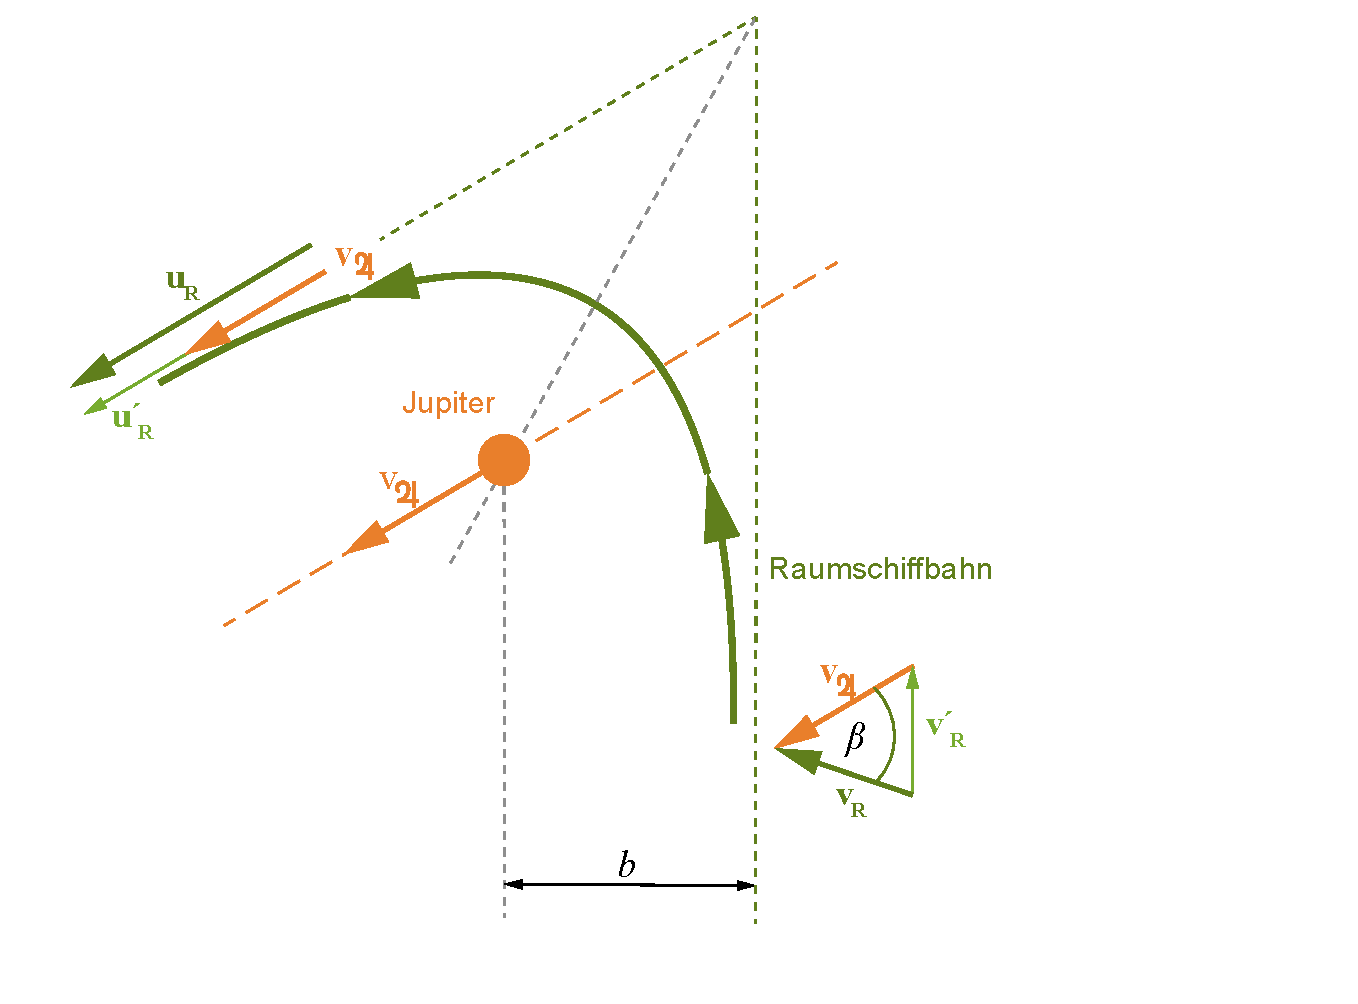
\includegraphics[width=\textwidth]{Lsg_SwingBy.pdf}%
\caption[Geometrie des Swing-By-Man�vers am Jupiter]{Geometrie des Swing-By-Man�vers am Jupiter}
\label{abb:bew_Lsg_SwingBy}
\end{figure}

Zur Berechnung der erreichbaren Geschwindigkeits�nderung braucht man:\\
\begin{tabular}{L{1.5cm}L{10.0cm}}
	$\vec{v}_R$,$\vec{u}_R$ & die Anfangs- bzw. Endgeschwindigkeit des Raumschiffs in $\vec{\Sigma}_\text{L}$, wenn es in den Gravitationsbereich des Jupiters kommt bzw. diesen verl�sst,  \\ 
	$\vec{v}'_R$,$\vec{u}'_R$ & die Anfangs- bzw. Endgeschwindigkeit des Raumschiffs in $\vec{\Sigma}'$, wenn es in den Gravitationsbereich des Jupiters kommt bzw. diesen verl�sst,  \\ 
  $\vec{v}_{\jupiter}$ & die Bahngeschwindigkeit des Jupiters zur Zeit des Vorbeifluges der Raumsonde, die f�r diesen Zeitabschnitt als konstant angesehen wird, \\ 
  $b$ & den Sto�parameter, d.h. den Abstand der einfallenden Asymptote vom Planetenzentrum. \\ 
\end{tabular}\\
Die Geschwindigkeiten der Raumsonde im System $\vec{\Sigma}'$, das hier das Schwerpunktsystem des Jupiters ist, sind gestrichen gekennzeichnet, die ungestrichenen Gr��en beziehen sich auf das Laborsystem $\vec{\Sigma}_\text{L}$, welches das KOS der ruhenden Sonne ist. \\
Es gilt dann:
		\begin{align*}
				\vec{v}_\text{R}&=\vec{v}_\text{R}'+\vec{v}_{\jupiter} \,,~~~~~\vec{u}_\text{R}=\vec{u}_\text{R}'+\vec{v}_{\jupiter} \,. 
		\end{align*}
\newpage
F�r die asymptotischen Hyperbelgeschwindigkeiten (\figref{bew_Lsg_SwingBy}) gilt:
		\begin{align}
				|\vec{v}_\text{R}'|=|\vec{u}_\text{R}'|=\sqrt{{v_\text{R}}^2+{V_{\jupiter}}^2-2v_\text{R}v_{\jupiter}\cos\beta} \,, \label{eq:bew_lsg_SwingBy05}
		\end{align}
worin $\beta$ der Winkel zwischen $\vec{v}_\text{R}$ und $\vec{v}_{\jupiter}$ ist. \\
In den Kapiteln Himmelsmechanik
und Astrodynamik (Band II, Kapitel 3 und 4) wird genauer gezeigt, wie man die Geschwindigkeiten von Planeten und Raumsonden 
bei einer Missionsplanung berechnet.
Hier machen wir nur eine Absch�tzung aus der Umlaufszeit und dem mittleren Bahnradius.
		\begin{align}
				v_{\jupiter} = \frac{2\pi \, a_{\jupiter} }{T_{\jupiter}}  = \frac{2\pi\cdot 5.2\cdot149\cdot10^6 \, \mathrm{km}}{11.9\cdot 365\cdot 86400 \,\mathrm{s}} \approx \SI{12.9}{km\per\second} \,.
		\end{align}
Die maximale Geschwindigkeit des Raumschiffes k�nnen wir wie folgt absch�tzen.
Auf der Erdbahn muss das Raumschiff, die Fluchtgeschwindigkeit
\begin{align*}
	v_\text{F} = \sqrt{\frac{2 G m_{\astrosun}}{a_{\earth}}} \approx 42.1 \,\mathrm{km\,s^{-1}}
\end{align*}
mitbekommen, um unser Sonnensystem verlassen zu k�nnen. %In der Realit�t wird man diesen Wert mit der heutigen Raketentechnik nicht erreichen. \\
Aus dem Energieerhaltungssatz folgt dann in Bahnn�he des Jupiters ($a_{\jupiter} \approx 5.2 a_{\earth}$) die Geschwindigkeit der Raumsonde:
		\begin{align}
				v_\text{R}\approx v_\text{F}\sqrt{\frac{1}{5.2}}\approx 18.5 \,\mathrm{km\,s^{-1}} \,. \label{eq:bew_lsg_SwingBy05a}
		\end{align}
F�r den Winkel $\beta$ k�nnen wir aus der \figref{bew_Lsg_SwingBy} entnehmen:
		\begin{align}
				\cos\beta=\frac{\vec{v_\text{R}}v_{\jupiter}}{|\vec{v_\text{R}}|\cdot|\vec{v_{\jupiter}}|} = \frac{v_\text{RJ}}{v_\text{R}} \,, \label{eq:bew_lsg_SwingBy05b}
		\end{align}
worin $v_\text{RJ}$ die Projektion von $\vec{v_\text{R}}$ auf die Jupiterbahn ist.
Wegen der Drehimpulserhaltung der Raumsonde bezogen auf die Sonne gilt:
		\begin{align}
				L=\underbrace{m\, a_{\jupiter} \, v_\text{RJ}}_{\substack{\text{Drehimpuls bei \linebreak Jupiter}}}=\underbrace{m \, a_{\earth}\,v_\text{FL} }_{\substack{\text{Drehimpuls bei \linebreak Start Erde}}} ~ \nonumber \\
				\longrightarrow v_\text{RJ} = v_\text{F} \frac{a_{\earth}}{a_{\jupiter}}= \frac{1}{5.2}\,v_\text{F} \approx 8.1 \,\mathrm{km \, s^{-1}} \,. \label{eq:bew_lsg_SwingBy05c}
		\end{align}
Damit erhalten wir aus \eqref{eq:bew_lsg_SwingBy05a} $\beta= \arccos\ \lk \sqrt{1/5.2} \rk \approx 64\degree$ \bzw aus \eqref{eq:bew_lsg_SwingBy05}:
		\begin{align*}
				|u_\text{R}'| \approx 17.3 \,\mathrm{km \, s^{-1}}\,.
		\end{align*}
F�r den Geschwindigkeits�bertrag gemessen im $\vec{\Sigma}_\text{L}$ Koordinatensystem erreicht man den Maximalwert, wenn $\vec{u_\text{R}}$ parallel zu $\vec{v_{\jupiter}}$ liegt:
		\begin{align*}
				u_\text{R} &\approx u_\text{R}'+v_{\jupiter} \approx 17.3\, \mathrm{km \, s^{-1}} + 12.9 \,\mathrm{km \, s^{-1}} \approx 30.2\, \mathrm{km \, s^{-1}} \,. 
		\end{align*}
Die Ausgangsgeschwindigkeit ist damit deutlich gr��er ist als die beim Eingang in den Jupiterbereich ($18.5\, \mathrm{km \, s^{-1}}$).
Die Weiterreise zum Saturn ($a_{\saturn} = 9.5\, a_{\earth}$) oder Pluto ($a_{\pluto} = 39.5 \,a_{\earth}$) verk�rzt sich damit um $\approx$ 0.5 \bzw 3.5 Jahre.\\

\newpage
\subprob{(Zusatz) Alternative Betrachtung des Swing-By-Man�vers}

Man kann das Problem auch einfach als Energietransferbetrachtung eines elastischen Sto�es betrachten. 
Allerdings k�nnen wir nicht einfach die Energie�bertragung nach \eqref{eq:bew_Streuung3} nehmen, da diese f�r eine ruhende Masse $m_2$ hergeleitet worden war.
In unserem Fall ist $m_\text{L}= m_{\jupiter}$ und bewegt sich aber im Labor(Sonnen)system mit ca. $v_{\jupiter} = \SI{12.9}{\km\per\second}$.
Wir m�ssen deshalb \eqref{eq:bew_Streuung3} auf den Fall erweitern, dass sich beide Massen bewegen.
Dann braucht man aber zur Auswertung der Gleichung immer noch den Streuwinkel $\vartheta'$, der sich f�r diesen Fall aus der Bewegung im Zentralkraftfeld ableiten l�sst. Dies wird in der Astrodynamik im Band II, Kapitel 4 im  Detail ausgef�hrt.\\
Man kann nat�rlich auch die Bewegungsgleichung der Sonde im Zentralkraftfeld des sich bewegenden Jupiter mit den entsprechenden Anfangsbedingungen numerisch integrieren, um so die genaue Bahn auch unter Einrechnung von St�rgr��en zu berechnen. Es sei auf die numerische Behandlung der Rutherford-Streuung im Kapitel \ref{kap:bew_scatter_problems} \bzw des Swing-By-Man�vers in der Astrodynamik im Band II, Kapitel 4 verwiesen.

\end{subprobs}
\end{sol} 
%\href{PhysikUncut_Part1.pdf#prb:bew_SwingBy}{\textcolor{blue} {$\rightarrow$ zur \probref{bew_SwingBy}.}}\\
\textcolor{blue} {$\rightarrow$ zur} \probref{bew_SwingBy}.\\
\noindent\rule[1ex]{\textwidth}{0.5pt}  \newpage
\medskip

%-----------------------------------------------------------------------------------------------------------
\hypertarget{lsg:bew_Billardspiel}{}
\begin{sol}{prob:bew_Billardspiel}\label{lsg:bew_Billardspiel} %�bung10
\textbf{Billardspiel} \\
\begin{figure}[H]
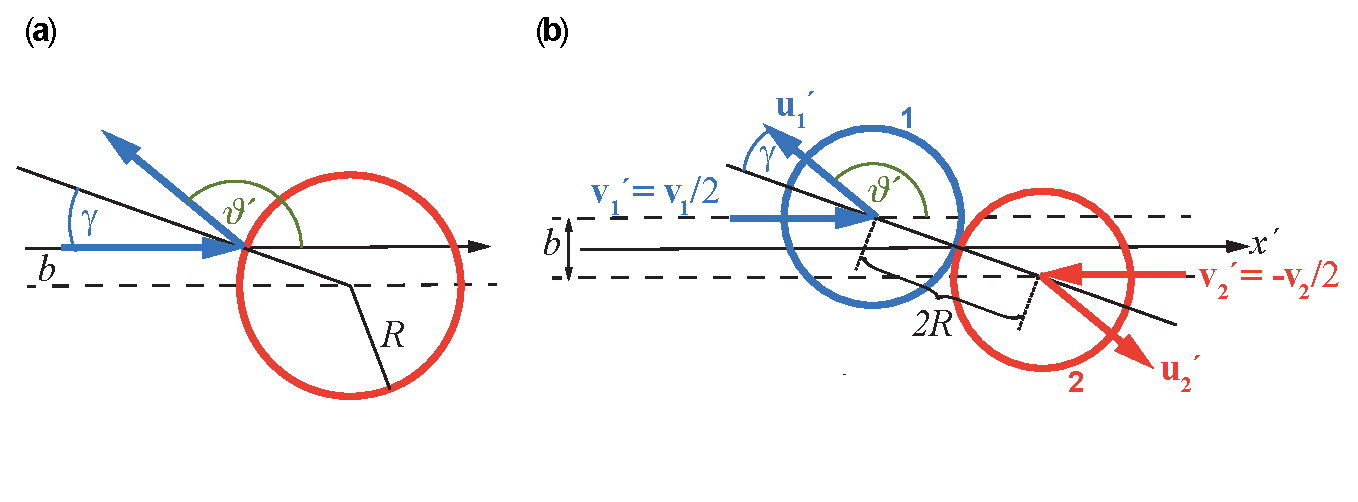
\includegraphics[width=\textwidth]{Billardspiel02.pdf}
\caption[Reflexion eines Teilchens an einer Kugeloberfl�che]{\fa Reflexion eines Teilchens an einer Kugeloberfl�che und \fb Geometrie zweier Billardkugeln im Moment des Zusammensto�es im Schwerpunktsystem $\vec{\Sigma}'$} 
\label{abb:bew_Billardspiel02}
\end{figure}
\begin{subprobs}
\subprob{Wirkungsquerschnitte bei idealer Reflexion.}
Wir betrachten zun�chst die Reflexion eines beliebig kleinen Teilchens an einer Kugeloberfl�che (\figref{bew_Billardspiel02} a). 
Aus der Geometrie erkennt man:
	\[\sin\gamma = \frac{b}{R} \quad  \text{und} \quad \vartheta' = \pi - 2\gamma = \pi - 2 \arcsin\frac{b}{R} \]
	\[\rightarrow b(\vartheta') = R \sin \frac{\pi - \vartheta'}{2} = R \cos \frac{\vartheta'}{2}\,. \]
Mit \eqref{eq:bew_Streuung16} folgt daraus der differentielle Wirkungsquerschnitt:
\begin{align}
	\frac{\D \sigma'}{\D \Omega}  \:=  \frac{1}{2 \sin\vartheta'} \left| \frac{\D b^2(\vartheta')}{\D\vartheta'} \right| = \frac{1}{2 \sin\vartheta'}  \, R^2  \, \cos \frac{\vartheta'}{2}  \, \sin \frac{\vartheta'}{2} = \frac{1}{4} R^2 \,. 
	\label{eq:bew_Billard01}
\end{align}
Der totale Wirkungsquerschnitt ergibt sich durch Integration �ber den Raumwinkel:
		\[\sigma' \:= \int \frac{\D \sigma'}{\D \Omega}  \, \D \Omega = 2 \pi \int\nolimits_{0}^{\pi} \frac{\D \sigma'}{\D \Omega} \sin\vartheta'  \, \D \vartheta' = \frac{\pi R^2}{2} \int\nolimits_{0}^{\pi} \sin\vartheta'  \, \D \vartheta' = \pi R^2 \,.
	\]
Wie nicht anders zu erwarten, ist dies die Querschnittsfl�che der Kugel.

\newpage
\subprob{Wirkungsquerschnitte beim Sto� zweier Kugeln.}
Wir gehen nun zu zwei Kugeln �ber und betrachten \figref{bew_Billardspiel02}\,b.
Wir k�nnen das Ergebnis von Teilaufgabe 1 verwenden, in dem wir $\hat{R} = R_1 + R_2$ setzen und erhalten:
	\[\frac{\D \sigma'}{\D \Omega}  \:=  \frac{1}{4} \hat{R}^2 \,.
	\]
F�r die Umrechnung ins Laborsystem gilt die Gleichung \eqref{eq:bew_Streuung7}, die wir wie folgt umformen:
\begin{align}
	\tan^2\vartheta \lk \cos\vartheta' + \frac{m_1}{m_2} \rk^2 &= 1 -\cos^2\vartheta'  \nonumber \\
	\sin^2\vartheta \lk \cos^2\vartheta' + 2  \, \frac{m_1}{m_2} \, \cos\vartheta' + \lk \frac{m_1}{m_2} \rk^2 \rk &= \cos^2\vartheta -\cos^2\vartheta\cos^2\vartheta' \nonumber \\
	\rightarrow \cos\vartheta' = -\frac{m_1}{m_2} \sin^2\vartheta + \cos\vartheta \sqrt{1 - \lk\frac{m_1}{m_2}\rk^2 \sin^2\vartheta} \,.\label{eq:bew_Billard02}
\end{align}
Daraus berechnet man leicht:
	\[
	\frac{\D \sigma}{\D \Omega} = \frac{\D \sigma'}{\D \Omega} \left| \frac{\D \cos\vartheta'}{\D \cos\vartheta} \right| = \lek 2 \frac{m_1}{m_2} \cos\vartheta + \frac{1 + \lk\frac{m_1}{m_2}\rk^2 \cos(2\vartheta)} {\sqrt{1 - \lk\frac{m_1}{m_2}\rk^2 \sin^2\vartheta}} \rek \frac{\D \sigma'}{\D \Omega} \,,
\]
woraus man mit \eqref{eq:bew_Streuung17} den differentiellen Wirkungsquerschnitt im Laborsystem erh�lt.
F�r $m_1 = m_2$ gilt $\hat{R} = 2R$ und man erh�lt:
	\[\frac{\D \sigma}{\D \Omega} = R^2 \lk 2\cos\vartheta + \frac{1+\cos(2\vartheta)}{\cos\vartheta} \rk = 4 R^2 \cos\vartheta \,.
\]
Die Streuwinkel im Laborsystem als Funktion des Sto�parameters ergeben sich dann zu:
\begin{align}
		\vartheta_1 = \arctan\frac{\sin\vartheta'}{\cos\vartheta'+1} ~~\text{und} ~~ \vartheta_2 = 90\degree - \vartheta'/2 \,. \label{eq:bew_Billard03}
\end{align}
\subprob{Berechnung des Sto�parameters.}
Um den Sto�parameter zu berechnen, bei dem die gesto�ene Kugel unter einem Winkel von $60 \degree$ wegrollt, wird \eqref{eq:bew_Billard02} nach $\vartheta'$ gel�st.
Wir erhalten: $\vartheta' = 2 \vartheta_1 = 120\degree$, woraus $\vartheta_2 = 30\degree$ folgt.
Das Ergebnis h�tte man nat�rlich auch direkt aus dem Impuls- und Energieerhaltungssatz ableiten k�nnen, es ging hier aber darum, die grunds�tzliche Vorgehensweise bei Streuproblemen zu beleuchten.
Welche Energie wird �bertragen?
Hier benutzen wir \eqref{eq:bew_Streuung9} und erhalten einen Energie�bertrag auf Kugel 2 von:
\begin{align}
	\frac{\Delta T}{T_1^{\text{(init)}}} = \frac{1}{2} \lk \cos\vartheta' -1 \rk =  -\frac{3}{4} = -75\,\% ~, \label{eq:bew_Billard04}
\end{align}
was bedeutet, dass $75\,\%$ der kinetischen Energie von Kugel 1 auf Kugel 2 �bertragen werden.
\end{subprobs} 
Die Ergebnisse der Rechnungen sind in \mlbewref{Billardspiel.m} ausgef�hrt und in \figref{bew_Billardspiel03} gezeigt.\\

\begin{figure}[H]
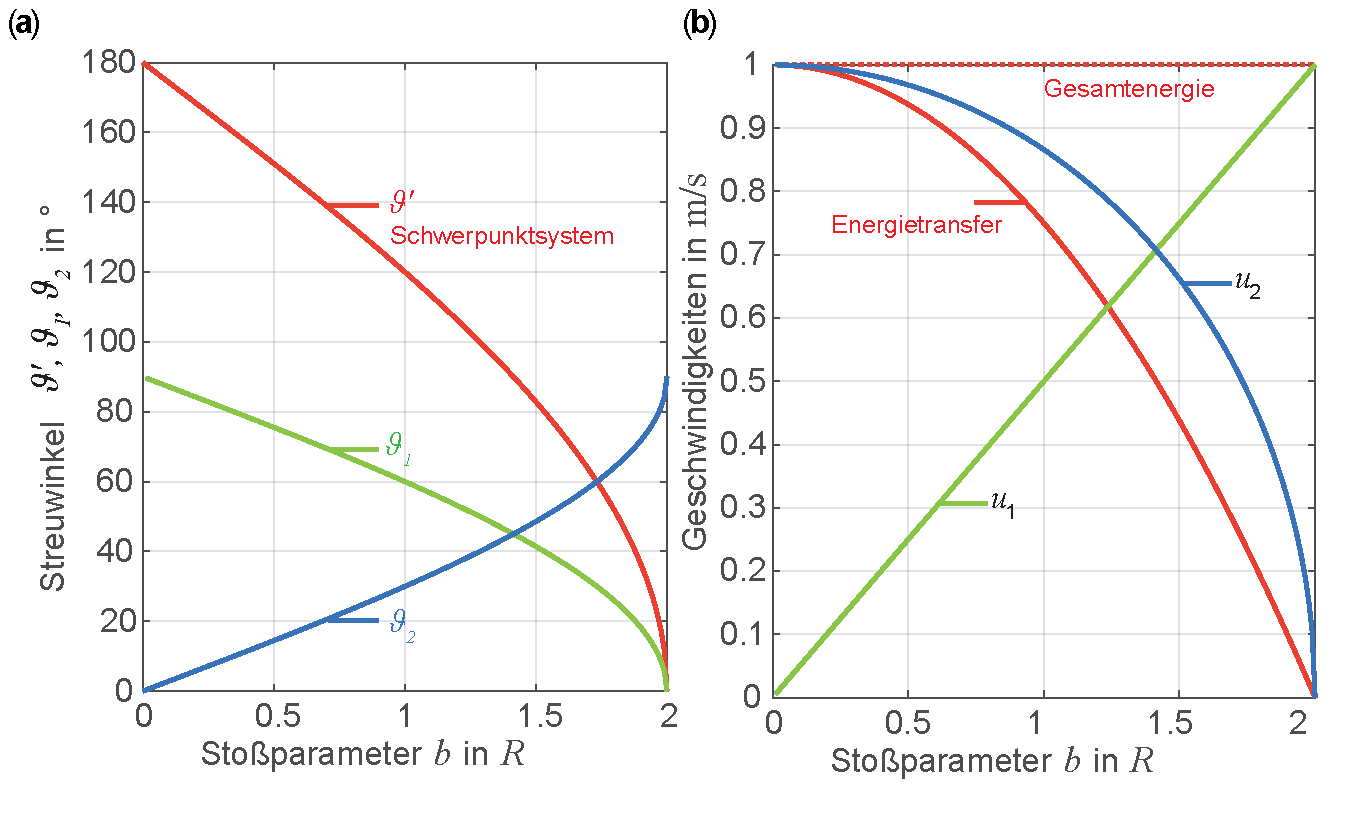
\includegraphics[width=\textwidth]{Billardspiel03.pdf}
\caption[Streuwinkel und Geschwindigkeiten zweier Billardkugeln]{\fa Streuwinkel und \fb Geschwindigkeiten und Energietransfer nach Zusammensto� zweier identischer Billardkugeln, von denen eine ruht und die andere mit $v=\SI{1}{\metre\per\second}$ gesto�en wird}
\label{abb:bew_Billardspiel03}
\end{figure}

\end{sol} 
%\href{PhysikUncut_Part1.pdf#prb:bew_Billardspiel}{\textcolor{blue} {$\rightarrow$ zur \probref{bew_Billardspiel}.}}\\
\textcolor{blue} {$\rightarrow$ zur} \probref{bew_Billardspiel}.\\
\noindent\rule[1ex]{\textwidth}{0.5pt}  \newpage

%-----------------------------------------------------------------------------------------------------------
\hypertarget{lsg:bew_HillLagrangePkt}{}
\begin{sol}{prob:bew_HillLagrangePkt}\label{lsg:bew_HillLagrangePkt} %�bung11
\textbf{Hill-Kurve und Lagrange-Punkte.} \\ \\
	F�r das Sonne-Planeten-System (z.B. Sonne-Erde) ist die Geometrie gegeben durch 
	\[  1 - q = \frac{m_2}{m_2 + m_1} = \frac{1}{1+ {m_1}/{m_2}} < 1
	\]
	%und den Ortsvektoren
	%\[\vec{r_1} = \lk (q-1)a,0,0 \rk  \qquad , \qquad \vec{r_2}=\lk qa,0,0 \rk \] 
	%und $\vec{\omega}=(0,0,\omega)$.
	% Vektorschreibweise:
		und den Ortsvektoren $\vec{r}_1, \vec{r}_2$
	\[
		\vec{r_1} = \lk \begin{array} {c}
	 	(q-1)\,a \\ 0\\ 0
	 \end{array} \rk, \qquad
		\vec{r_2} = \lk \begin{array} {c}
	 	q\,a \\ 0\\ 0 
		\end{array} \rk  \quad \text{sowie der Umlaufkreisfrequenz} \quad
		\vec{\omega} = \lk \begin{array} {c}
	 	0 \\ 0\\ \omega 
	 \end{array} \rk \,.
	\]
	Hierbei haben wir die Bahnebene als $x$-$y$-KOS verwendet und den Nullpunkt in den Schwerpunkt des Systems gelegt.
	Wir k�nnen damit das effektive Potential $\hat{U}_\text{eff}$ berechnen, welches auf eine Testmasse (z.B. Satelliten) $m_3$ und auf die Gravitationskonstante $G$ normiert ist:
	\[\hat{U}_\text{eff}(x_3,y_3) = \frac{U_\text{eff}}{G m_3} = -\frac{m_1}{d_1(x_3,y_3)} - \frac{m_2}{d_2(x_3,y_3)} - \frac{m_1 + m_2}{2a^3}({x_3}^2 + {y_3}^2) ~,
	\]
	wobei
	\begin{align*}
		d_1 &= \sqrt{\lk x_3 - (q-1)\,a\rk^2 + {y_3}^2} = d_1(x_3,y_3) \qquad \text{und} \\
		d_2 &= \sqrt{\lk x_3 - q\,a\rk^2 + {y_3}^2} = d_2(x_3,y_3)~.
	\end{align*}
	Die entsprechende allgemeine Rechnung ist in \mlbewref{LagrangePunkte.m} ausgef�hrt.
	In \figref{bew_3KoerperP03} sind die Lagrange-Punkte und Hill-Kurven f�r ein dem Sonne-Jupiter-�hnlichen System mit $m_1/m_2 = 1000$ und einem hypothetischen System mit einem Massenverh�ltnis von $m_1/m_2 = 10$ dargestellt. 
	Auch f�r  das Erde-Mond-System (mit einem Massenverh�ltnis von $m_1/m_2 \approx 333 000$) bleibt die grunds�tzliche geometrische Lage der Lagrange-Punkte erhalten. 
	Sie sind jeweils lokale Maxima des effektiven Potentials, die aber mathematisch instabile Gleichgewichtspunkte sind, wie man durch nochmalige Ableitung von ${\partial}/{\partial \vec{r}_3} \,\lk U_\text{eff} \rk$ zeigen kann.\\
Dass sich \zb ein Raumschiff dennoch relativ stabil
an einem Lagrange-Punkt aufhalten kann, wird in der Astrodynamik im Band II, Kapitel 4 durch eine entsprechende
Stabilit�tsanalyse gezeigt.
Ursache daf�r ist das Wirken der Coriolis-Kraft in den Bewegungsgleichungen \eqref{eq:bew_red3KP07}.\\

\begin{figure}[H]
\includegraphics[width=\textwidth]{LagrangePt.pdf}
\caption[Lagrange-Punkte und Hill-Kurven Sonne-Planeten-Satelliten-Systeme]{Lagrange-Punkte und Hill-Kurven f�r zwei Sonne-Planeten-Satelliten-Systeme} 
\label{abb:bew_3KoerperP03}
\end{figure}

\end{sol} 
%\href{PhysikUncut_Part1.pdf#prb:bew_HillLagrangePkt}{\textcolor{blue} {$\rightarrow$ zur \probref{bew_HillLagrangePkt}.}}\\
\textcolor{blue} {$\rightarrow$ zur} \probref{bew_HillLagrangePkt}.\\
\noindent\rule[1ex]{\textwidth}{0.5pt}  \newpage

%-----------------------------------------------------------------------------------------------------------
\hypertarget{lsg:bew_gezeiten01}{}
\begin{sol}{prob:bew_gezeiten01}\label{lsg:bew_gezeiten01} %�bung12
\textbf{Gezeitenkr�fte.} \\

Wir wollen die Verformung eines Masserings unter dem Einfluss von Gezeitenkr�ften berechnen. Den Ring beschreiben wir als Anordnung von 36 Testmassen, die im Schwerefeld einer gro�en Masse frei fallen. Wir betrachten dazu die Geometrie nach \figref{bew_lsggezeiten01}. \\
Wir k�nnen die Massen $m_1$ bis $m_{17}$ und $m_{19}$ bis $m_{35}$ wie folgt behandeln:
\begin{align*}
    \varphi_i\lk 0\rk = i\cdot 10\degree && i = 1\ldots 17, 19\ldots 35
\end{align*}
Nach dem Sinussatz gilt zum Zeitpunkt $t=0$:
\begin{align}
    \frac{\sin\alpha_i}{R} &= \frac{\sin\varphi_i\lk 0\rk}{r_i\lk 0 \rk}  \label{eq:bew_lsggezeiten01} \\
    \rightarrow ~~~~ \sin\alpha_i &= \frac{R}{r_0}\,\frac{\sin\varphi_i\lk 0\rk}{\sqrt{q-2\,\frac{R}{r_0}\,\cos\varphi_i\lk 0\rk + \frac{R^2}{r_0{}^2}}}\;. \nonumber
\end{align}
Der Winkel $\alpha_i$ ist f�r jede Masse konstant �ber die Zeit, wenn wir wie angenommen alle $m_i \ll M$ annehmen.\\
Die Newtonschen Bewegungsgleichungen lauten dann im gew�hlten KOS nach \figref{bew_lsggezeiten01}:
\begin{align}
\begin{split}
    \ddot{x}_i &= -\frac{M\,G}{x_i{}^2+z_i{}^2}\,\sin\alpha_i\,, \\
    \ddot{z}_i &= -\frac{M\,G}{x_i{}^2+z_i{}^2}\,\cos\alpha_i\,.
\end{split} \label{eq:bew_lsggezeiten02}
\end{align}
Die Anfangsbedingungen sind gegeben durch:
\begin{align*}
    x_i\lk 0\rk &= R\,\sin\varphi_i \,,\\
    z_i\lk 0\rk &= r_0 - R\,\cos\varphi_i \,.
\end{align*}
F�r die Massen $m_0$, $m_{18}$ und $m_z$ vereinfacht sich das System, da $\alpha_0 = \alpha_{18} = \alpha_z = 0$ zu
\begin{align}
    \ddot{z}_i = -\frac{M\,G}{z_i{}^2}\,. \label{eq:bew_lsggezeiten03}
\end{align}
Wir l�sen die DGL-Systeme \eqref{eq:bew_lsggezeiten02} und \eqref{eq:bew_lsggezeiten03} numerisch (\mlbewref{Gezeitenkraefte.m}).
Die L�sung ist in \figref{bew_lsggezeiten01} dargestellt.
Wir erkennen wie sich der Ring verformt.
In unserem Fall, in dem wir $M\gg m$ angenommen haben und auch $r_0$ nur wenig gr��er als $R$ ist die Gezeitenkraft f�r die Masse $m_{18}$ deutlich kleiner als f�r die Masse $m_0$, $m_{17} < m_1$ \usW
Folglich verformt sich der Ring nicht zu einem Ellipsoid, sondern zu einer birnenf�rmigen Anordnung von Massen. \\

\begin{figure}[H]
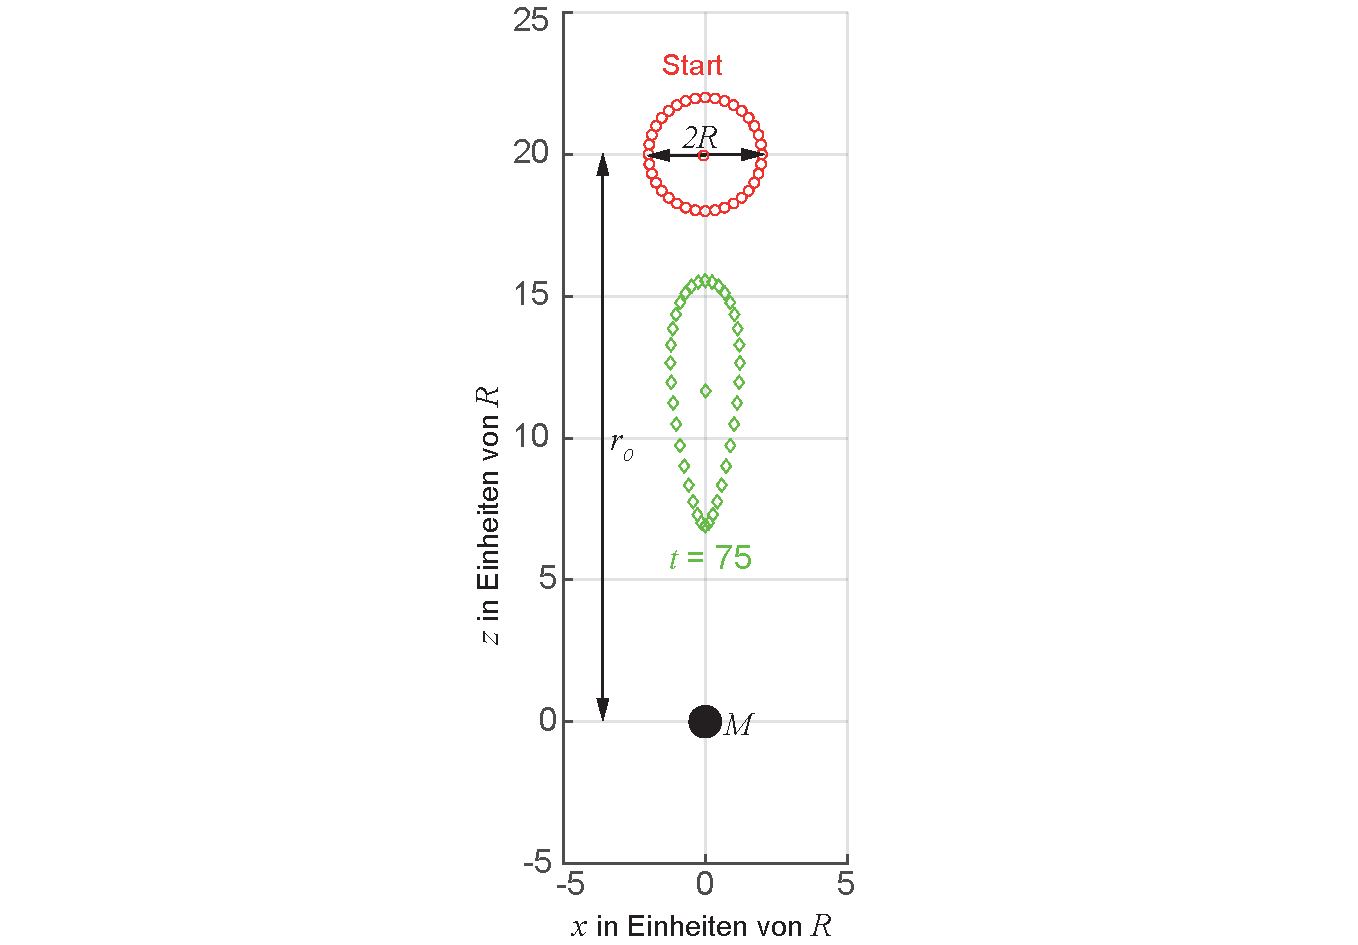
\includegraphics[width=\textwidth]{Gezeitenkraefte.pdf}
\caption[Gezeitenwirkung auf einen Ring]{Gezeitenwirkung auf einen Ring aus 36 Massepunkten. Parameter: $r_0 = 20 R, R = 2, M\,G = 1$}
\label{abb:bew_lsggezeiten01}
\end{figure}

F�r den mathematisch interessierten Leser geben wir noch eine analytische L�sung f�r \eqref{eq:bew_lsggezeiten03}, wobei diese nicht wirklich einen gro�en Vorteil bietet, da sie nur eine analytische L�sung f�r $t\lk z\rk$ liefert, man also auch noch numerisch die Umkehrfunktion $z\lk t\rk$  bestimmen muss. Wir schreiben dazu f�r \eqref{eq:bew_lsggezeiten03}:
\begin{align*}
    \ddot{z} &= \frac{A}{z^2} ~~~~ \text{mit} ~~~~ A=-M\,G \\
    A-\ddot{z}\,z^2 &= 0 ~~~~| \dot{z} ~~\rightarrow ~~ \frac{A\,\dot{z}}{z^2} = \dot{z}\,\ddot{z}
\end{align*}
Mit $\frac{\D}{\D t}\,\lk \dot{z}\rk^2 = 2\dot{z}\,\ddot{z}$ und $\frac{\D}{\D t}\,\lk -\frac{A}{z}\rk = \frac{A\,\dot{z}}{z^2}$ erhalten wir:
\begin{align*}
    C_1 -\frac{A}{z} = \frac{1}{2}\,\dot{z}^2\,,
\end{align*}
worin $C_1$ eine Integrationskonstante ist, die sich aus dem AB ergibt.
\begin{align*}
    \sqrt{2C_1 - \frac{2A}{z}} &= \dot{z}\,~~\rightarrow~~ \D t = \frac{\D z}{\sqrt{2C_1-\frac{2A}{z}}} = \frac{\D z}{\sqrt{2}\sqrt{C_1-\frac{A}{z}}}\,.
\end{align*}

\newpage
Aus Integraltafeln (\zb \cite{Gradshteyn1980}) finden wir 
\begin{align}
\begin{split}
    \int\limits_0^t \D t &= t = \int\limits_{z_0}^t \frac{\D z}{\sqrt{C_1 - \frac{A}{z}}} ~~~~~~~~ 2C_1 \rightarrow C_1 \\
    &= \frac{z\,\sqrt{C_1 - \frac{2A}{z}}}{C_1} + \frac{2A\,\arctan\lek \frac{\sqrt{C_1-\frac{2A}{z}}}{\sqrt{C_1}}\rek}{\sqrt{C_1{}^3}}
\end{split} \label{eq:bew_lsggezeiten04}
\end{align}
Wenn man $z\lk t \rk$ haben will, muss man wie gesagt \eqref{eq:bew_lsggezeiten04} ebenfalls numerisch l�sen. 

\end{sol} 
%\href{PhysikUncut_Part1.pdf#prb:bew_gezeiten01}{\textcolor{blue} {$\rightarrow$ zur \probref{bew_gezeiten01}.}}\\
\textcolor{blue} {$\rightarrow$ zur} \probref{bew_gezeiten01}.\\
\noindent\rule[1ex]{\textwidth}{0.5pt}  \newpage

%----------------------------------------------------------------------------------
\hypertarget{lsg:bew_Zwangsbedingungen}{}
\begin{sol}{prob:bew_Zwangsbedingungen}\label{lsg:bew_Zwangsbedingungen}%�bung13
\textbf{Zwangsbedingungen} 
\begin{subprobs}

\subprob{Perle auf 2D-Spirale}
	Wir betrachten zun�chst eine Spirale im $R^2$, d.h. in einer Ebene, auf der sich eine Perle bewegt.
        Die Spirale sei eine logarithmische Spirale:
	\begin{align*}
	r(\varphi) = a\mathrm{e}^{k\varphi}~.
	\end{align*} 
	Hierbei sind $a$ und $k$ feste Parameter.
	Daraus folgt die Zwangsbedingung: 
	\begin{align}
	a\mathrm{e}^{k\varphi}-r=0 \label{eq:lsg_bew_bed1}
	\end{align}
	$\rightarrow$ Kategorie: holonom-skleronom, ein Freiheitsgrad ($\varphi$).

\subprob{Perle auf eing�ngiger Helix}
	Wir betrachten nun eine Spirale im $R^3$, auch Helix genannt.
        Eine solche kann man sich vorstellen wie die in Kugelschreibern verbauten Stahlfedern.
        Die Bewegung einer Perle auf dieser Spirale kann in kartesischen Koordinaten wie folgt beschrieben werden: 
	\begin{align}
	\vec{x} =
	\begin{pmatrix}
	\varrho_0 \cos \varphi \\
	\varrho_0 \sin \varphi \\
	h \varphi
	\end{pmatrix}.
	\label{eq:lsg_bew_log_helix1}
	\end{align}
	Die beiden Zwangsbedingungen f�r Zylinderkoordinaten lauten:
	\begin{align}
	\varrho - \varrho_0 &= 0  &  z - h \varphi &= 0 \,. \label{eq:lsg_bew_log_helix2}
	\end{align}
	Dabei ist $h$ die Gangh�he der Helix und $\varphi$ als Winkel (in Bogenma�) die freie Variable.\\
	$\rightarrow$ Kategorie: holonom-skleronom, ein Freiheitsgrad ($\varphi$).

\subprob{Sph�risches Pendel}
	Der Massepunkt eines sph�rischen Pendels bewegt sich auf einer Kugeloberfl�che.
        Der Abstand zum Mittelpunkt dieser Kugel betr�gt damit f�r jeden m�glichen Aufenthaltsort des Massepunktes $R$.
        Dies ergibt die einfache Zwangsbedingung:
	\begin{align}
	x^2+y^2+z^2-R^2=0 \,, \label{eq:lsg_bew_SPen}
	\end{align}
	bzw. in sph�rischen Koordinaten: $r - R =0$.
        Es verbleiben zwei Freiheitsgrade.
	Als freie bzw. verallgemeinerte Koordinaten werden die beiden Winkel $\varphi$ und $\vartheta$ gew�hlt.
	\\
	$\rightarrow$ Kategorie: holonom-skleronom, zwei Freiheitsgrade ($\varphi$) und ($\vartheta$).

\begin{figure}[H]
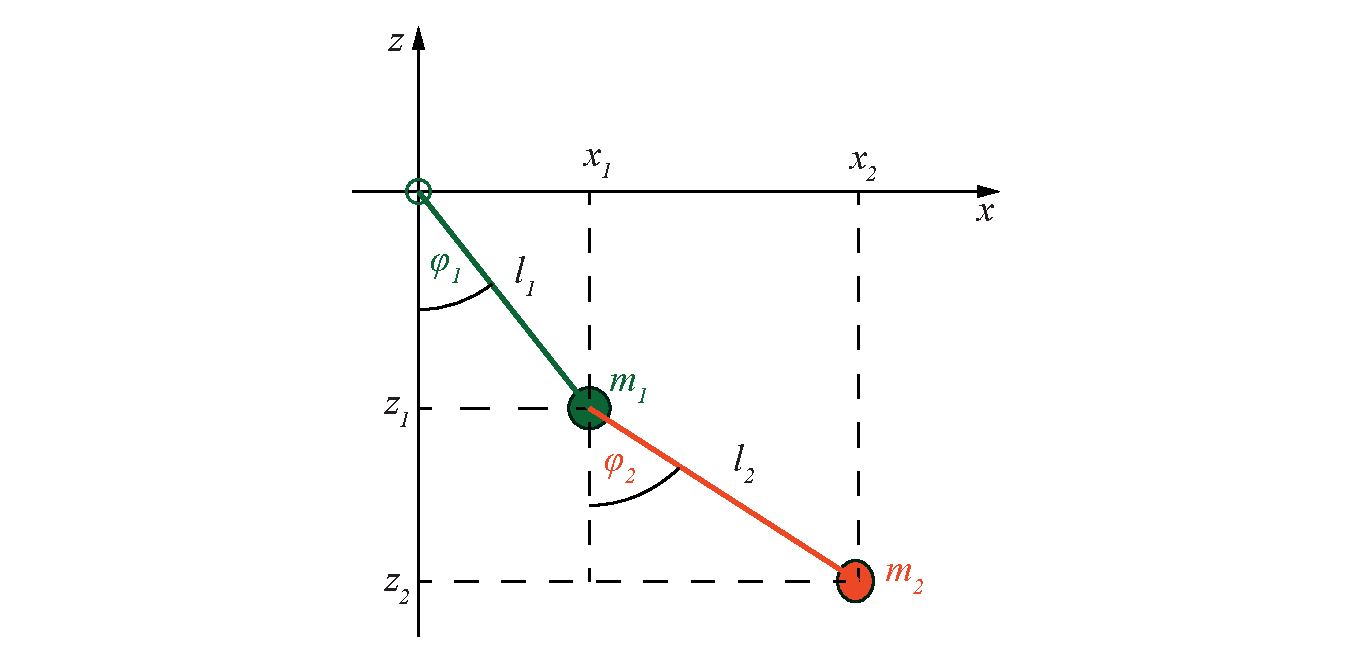
\includegraphics[width=\textwidth]{UebungDoppelpendel.pdf}%
\caption[Doppelpendel]{Doppelpendel}
\label{abb:bew_lsg_Doppelpendel}
\end{figure}

\subprob{Doppelpendel}
	Die Bewegung soll in der $x$-$z$-Ebene erfolgen.
        Um die Zwangsbedingungen eines (ebenen) Doppelpendels aufzustellen, betrachten wir zun�chst das einfaches Pendel mit dem Massepunkt $m_1$ und den kartesischen Koordinaten $x_1,y_1,z_1$.
        Dieser befindet sich im Abstand $l_1$ zum Aufh�ngepunkt.
        Daraus folgt die Zwangsbedingung:
	\begin{align}
		x_1^2+z_1^2-l_1^2=0 \,. \label{eq:lsg_bew_DPen1}
	\end{align}
	Wir betrachten nun einen zweiten Massepunkt $m_2$ mit den Koordinaten $x_2,y_2,z_2$, der �ber die feste  L�nge $l_2$ mit $m_1$ verbunden ist.
        Daraus folgt mit dem Abstand der beiden Punkte die zweite Zwangsbedingung:
	\begin{align}
	\Delta x^2 + \Delta z^2 &= l_2^2 \nonumber \\
	(x_2-x_1)^2 + (y_2-y_1)^2 - l_2^2 &= 0 \,. \label{eq:lsg_bew_DPen4}
	\end{align}
	Es gibt f�r die Bewegung in der $x$-$z$-Ebene also zwei Zwangsbedingungen und somit $4 - 2 = 2$ Freiheitsgrade.
        F�r diese bieten sich als generalisierte Koordinaten die Winkel $\varphi_1$ und $\varphi_2$ an.
        Die Transformation lautet:
	\begin{align*}
	\vec{r}_1 &= \begin{pmatrix} 
	l_1 \sin\varphi_1 \\ 
	0 \\ 
	-l_1 \cos\varphi_1  
	\end{pmatrix} & 
	\vec{r}_2 &= \begin{pmatrix} 
	l_1 \sin\varphi_1 + l_2 \sin\varphi_2 \\
	 0 \\
	  -l_1 \cos\varphi_1 - l_2 \cos\varphi_2 
	  \end{pmatrix}.
	\end{align*}
	$\rightarrow$ Kategorie: holonom-skleronom, zwei Freiheitsgrade ($\varphi_1$) und ($\varphi_2$).

\newpage
\subprob{Pendel mit vertikal schwingender Aufh�ngung}
	Das in der $x$-$z$-Ebene schwingende Pendel mit der L�nge $l$ ist am Aufh�ngepunkt mit Koordinaten $x_\text{A}=0, z_\text{A}$ befestigt, welcher mit einer Frequenz $\Omega$ schwingt.
        Es ist also $z_\text{A}=A\sin(\Omega t - \varphi_\text{A})$.
        Der am unteren Ende h�ngende Massepunkt hat die Koordinaten $x, y$. 
	Als Zwangsbedingung gilt generell f�r das Pendel
	\begin{align}
	\lk x-x_\text{A} \rk^2+ \lk z-z_\text{A} \rk^2-l^2=0 \, \label{eq:lsg_bew_PvA1} 
	\end{align}
	mit den Transformationen
	\begin{align}
	x &= l\sin \varphi \nonumber \\
	z &= A\sin(\Omega t - \varphi_\text{A}) - l \cos\varphi \,. \label{eq:lsg_bew_PvA2}
	\end{align} 
	$\rightarrow$ Kategorie: holonom-rheonom, ein Freiheitsgrad ($\varphi$).

\subprob{Pendel mit horizontal schwingender Aufh�ngung}
	Analog zur vorherigen Aufgabe k�nnen wir nun f�r die Transformationen formulieren: 
	\begin{align}
	x &= A\sin(\Omega t - \varphi_\text{A}) + l \sin\varphi \nonumber \\
	z &= -l \cos\varphi\,. \label{eq:lsg_bew_PvA3}
	\end{align}
	$\rightarrow$ Kategorie: holonom-rheonom, ein Freiheitsgrad ($\varphi $).

\subprob{Stehendes Pendel mit vertikal schwingendem Boden}
	Dies ist die Umkehrung des h�ngenden Pendels mit vertikal schwingender Aufh�ngung. 
	\begin{align}
	x &= l\sin \varphi \nonumber \\
	z &= A\sin(\Omega t - \varphi_\text{A}) + l \cos\varphi \,. \label{eq:lsg_bew_PvA4}
	\end{align} 
	$\rightarrow$ Kategorie: holonom-rheonom, ein Freiheitsgrad ($\varphi $).

\subprob{Jo-Jo}
	Die Bewegung findet wieder in der $x$-$z$-Ebene statt.
        Die Koordinaten beschreiben den Mittelpunkt des Jo-Jos.
        Aus der \figref{bew_lsg_JoJo} ergeben sich direkt die Zwangsbedingungen:
	\begin{align}
	  x &= 0 \\
	  z + r \varphi &= 0 \, 	\label{eq:lsg_bew_PvA5}
	\end{align}
	wobei das $\varphi > 0$ f�r das aufsteigende und $\varphi < 0$ f�r das absteigende Jo-Jo ist.\\
	$\rightarrow$ Kategorie: holonom-skleronom, ein Freiheitsgrad ($\varphi$).

\begin{figure}[H]
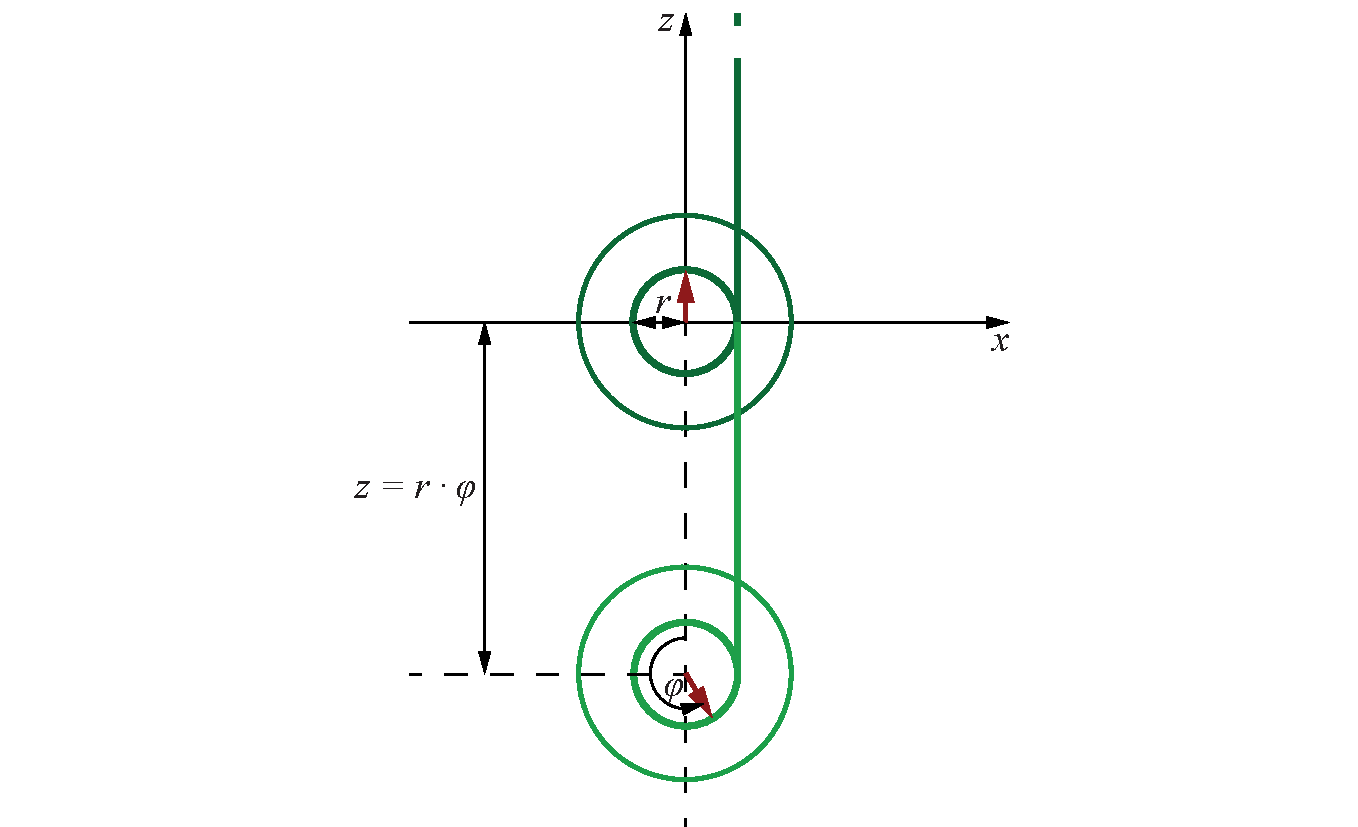
\includegraphics[width=\textwidth]{UebungJoJo.pdf}%
\caption[Akademisches Jo-Jo]{Akademisches Jo-Jo}
\label{abb:bew_lsg_JoJo}
\end{figure}

\end{subprobs} 
\end{sol} 
%\href{PhysikUncut_Part1.pdf#prb:bew_Zwangsbedingungen}{\textcolor{blue} {$\rightarrow$ zur \probref{bew_Zwangsbedingungen}.}}\\
\textcolor{blue} {$\rightarrow$ zur} \probref{bew_Zwangsbedingungen}.\\
\noindent\rule[1ex]{\textwidth}{0.5pt}  \newpage

%-----------------------------------------------------------------------------------------------------------
\hypertarget{lsg:bew_LagrangeII_a}{}
\begin{sol}{prob:bew_LagrangeII_a}\label{lsg:bew_LagrangeII_a}%�bung14
\textbf{Lagrange-Gleichung zweiter Art in Kugelkoordinaten} 
\begin{subprobs}
\subprob{Freies Teilchen}
Die Koordinaten des Massepunktes liegen in sph�rischen Koordinaten $(r, \vartheta, \varphi)$ vor.
Diese k�nnen wie folgt in kartesische Koordinaten umgerechnet werden:  
\begin{align}
x &= r\sin\vartheta\cos\varphi	\nonumber  \\ 
y &= r\sin\vartheta\sin\varphi	\nonumber  \\ 
z &= r\cos\vartheta \,. \label{eq:lsg_bew_LagrangeII_a_01}
\end{align}
Es gibt bei einem freien Teilchen keine Zwangsbedingungen, d.h. es m�ssen alle drei Koordinaten ber�cksichtigt werden.
Um die kinetische Energie $T$ in Kugelkoordinaten zu erhalten, m�ssen alle Koordinaten nach der Zeit abgeleitet werden, da alle drei Koordinaten von der Zeit abh�ngen.
Das Ergebnis lautet:
\begin{align}
\dot{x} &= \dot{r}\sin\vartheta\cos\varphi + r \, \dot{\vartheta}\cos\vartheta\cos\varphi - r \, \dot{\varphi}\sin\vartheta\sin\varphi \nonumber  \\ 
\dot{y} &= \dot{r}\sin\vartheta\sin\varphi + r \, \dot{\vartheta}\cos\vartheta\sin\varphi + r \, \dot{\varphi}\sin\vartheta\cos\varphi \nonumber  \\ 
\dot{z} &= \dot{r}\cos\vartheta - r \, \dot{\vartheta}\sin\vartheta \,. \label{eq:lsg_bew_LagrangeII_a_02}
\end{align}
Die kinetische Energie berechnet sich damit zu: 
\begin{align}
T &= \frac{m}{2} \lk\dot{x}^2 + \dot{y}^2 + \dot{z}^2\rk = \frac{m}{2} \lk\dot{r}^2 + r^2(\dot{\vartheta}^2 + \dot{\varphi}^2\sin^2\vartheta)\rk. \label{eq:lsg_bew_LagrangeII_a_03}
\end{align}
Der Umformungsschritt besteht vor allem in der mehrfachen Anwendung der trigonometrischen Identit�t $\sin^2x + \cos^2x = 1$.
Man erkennt, dass in \eqref{eq:lsg_bew_LagrangeII_a_03} keine gemischten Terme der Ableitungen der Ableitungen $\dot{r}, \dot{\vartheta}, \dot{\varphi}$ vorkommen. 
Mit dem Potential $U=U(r,\vartheta, \varphi)$ und der allgemeinen Lagrange-Funktion $\mathcal{L} = T - U$ erhalten wir die Lagrange-Gleichungen f�r die drei generalisierten Koordinaten $q = \{r, \vartheta, \varphi\}$ nach
\begin{equation}
	\frac{d}{dt} \frac{\d\mathcal{L}}{\d\dot{q}} - \frac{\d\mathcal{L}}{\d q} = 0~.
\end{equation}
Es ergeben sich dann folgende Lagrange-Gleichungen
\begin{align}
	\text{...f�r } r&:  & \frac{d}{dt}(m \, \dot{r})-m \, r \, (\dot{\vartheta}^2+\dot{\varphi}^2\sin^2\vartheta) &= \frac{\d U}{\d r}  \nonumber  \\ 
	\text{...f�r } \vartheta&:  & \frac{d}{dt}(m \, r^2 \, \dot{\vartheta}) - m r^2\dot{\varphi}^2\sin\vartheta \, \cos\vartheta &= \frac{\d U}{\d \vartheta}  \nonumber  \\ 
	\text{...f�r }\varphi&:  & \frac{d}{dt}(m \, r^2\sin^2\vartheta \, \dot{\varphi}) &= \frac{\d U}{\d \varphi} \,. \label{eq:lsg_bew_LagrangeII_a_04}
\end{align}
Diese Berechnung ist wesentlich einfacher als die in \probref{bew_KOS_Formel} durchgef�hrte Berechnung der Beschleunigung �ber die Ableitung der Geschwindigkeit. 

\newpage
\subprob{Teilchen auf Trichter}
Bewegt sich das Teilchen auf der Oberfl�che des kegelf�rmigen Trichters ist die Zwangsbedingung holonom und lautet mit $\vartheta_0$ als dem �ffnungswinkel des Kegels: 
\begin{align}
f = \vartheta - \vartheta_0 = 0 \,. \label{eq:lsg_bew_LagrangeII_a_05}
\end{align}
Dadurch gibt es nur noch zwei unabh�ngige Parameter, den Radius $r$ und den Winkel $\varphi$.
Die Lagrange-Funktion vereinfacht sich dann zu: 
\begin{align}
\mathcal{L} = \frac{m}{2}(\dot{r}^2 + r^2\dot{\varphi}^2 \, \sin^2\vartheta_0)-U(r) \,. \label{eq:lsg_bew_LagrangeII_a_06}
\end{align}
Die Lagrange-Gleichungen in $r$ und $\varphi$ lauten dann: 
\begin{align}
\frac{d}{dt}(m \, \dot{r}) - m \, r \, \dot{\varphi}^2 \, \sin^2\!\vartheta_0 + \frac{\d U}{\d r} &= 0 \nonumber  \\ 
\frac{d}{dt}(m \, r^2 \, \sin^2\!\vartheta_0 \, \dot{\varphi}) = \frac{d}{dt}p_\varphi &= 0 \,. \label{eq:lsg_bew_LagrangeII_a_07}
\end{align}
Der konjugierte Impuls $p_\varphi$ (entspricht hier dem Drehimpuls) ist erhalten und kann verwendet werden, um $\dot{\varphi}$ aus der Bewegungsgleichung f�r $r$ zu eliminieren: 
\begin{align}
\dot{\varphi} = \frac{p_\varphi}{m \, r^2 \, \sin^2\!\vartheta_0} \,. \label{eq:lsg_bew_LagrangeII_a_08}
\end{align}
Wir verwenden wieder das effektive Potenzial $U_\text{eff}$ aus \eqref{eq:bew_Eff_Potential} und schreiben obige Gleichung als: 
\begin{align}
m \, \ddot{r} &= -\frac{\d U}{\d r} + \frac{{p_\varphi}^2 m \, r \, \sin^2\!\vartheta_0}{m^2 \, r^4 \, \sin^4\!\vartheta_0} \nonumber  \\
&= -\frac{\d}{\d r} U + \frac{{p_\varphi}^2}{m \, r^3 \, \sin^2\!\vartheta_0} \nonumber  \\
&= -\frac{\d}{\d r} \lk U + \frac{{p_\varphi}^2}{2m \, r^2 \, \sin^2\!\vartheta_0} \rk = -\frac{\d}{\d r} U_\text{eff} \,. \label{eq:lsg_bew_LagrangeII_a_09}
\end{align}
Interessanterweise f�hrt diese Gleichung f�r $\vartheta_0=90\degree$ genau auf die beschreibenden Formeln des Zweik�rperproblems, welches wir in Kap \ref{kap:bew_ZKP_NZKF} behandelt haben.
\end{subprobs}
\end{sol} 
%\href{PhysikUncut_Part1.pdf#prb:bew_LagrangeII_a}{\textcolor{blue} {$\rightarrow$ zur \probref{bew_LagrangeII_a}.}}\\
\textcolor{blue} {$\rightarrow$ zur} \probref{bew_LagrangeII_a}.\\
\noindent\rule[1ex]{\textwidth}{0.5pt}  \newpage

%-----------------------------------------------------------------------------------------------------------
\hypertarget{lsg:bew_LagrangeII_b}{}
\begin{sol}{prob:bew_LagrangeII_b}\label{lsg:bew_LagrangeII_b}%�bung15
\textbf{Lagrange-Gleichung erster Art und zweiter Art mit Reibung} 

\begin{subprobs}
\subprob{L�sung ohne Reibung.}

Die L�sungen finden sich in den ausf�hrlich kommentierten \mscren\mlbewref{Rollenpendel.m} und \mlbewref{PerleDraht.m}.

\subprob{L�sung mit Reibung.} 

Nun wollen wir uns dem etwas komplizierteren, aber daf�r realistischeren Fall zuwenden, dass in den Systemen Reibungskr�fte vorhanden sind.
\begin{enumerate}[a) ]
\item Perle auf Draht mit konstanter Drehzahl \\
	Die L�sungen f�r die Bewegungsgleichungen kann man direkt durch Erweiterung der numerischen L�sung nach \mlbewref{PerleDraht.m} erhalten.
	Dies ist in \mlbewref{PerleDrahtErweiterung.m} ausgef�hrt.
\item Perle auf Draht und Feder bzw. auf parabolisch gebogenem Draht \\
	Wir k�nnen jetzt noch als interessante Erweiterung annehmen, dass die Perle zus�tzlich durch eine mitrotierende Feder gehalten wird oder der Draht in Form einer parabolisch nach oben gebogenen Rollbahn gebogen ist.
        Dann muss die Lagrange-Funktion durch einen das jeweilige Potential beschreibenden Term $U(x_1)$ erweitert werden.
        Die Terme lauten 
	\[U(x_1) = \frac{k}{2}\lk x_1 - x_{1,\text{F}} \rk^2 \quad \text{bzw.}\quad  U(x_1) = \frac{m}{2} g x_1^2 \,.
	\]
	Die L�sung ist ebenfalls in \mlbewref{PerleDrahtErweiterung.m} ausgef�hrt.
\item Rollenpendel mit Reibung\\
	Wir starten von der Lagrange-Gleichung erster Art, da wir ja die Reibungskr�fte ber�cksichtigen wollen.
        F�r die Rollreibung der Masse $m_1$ ist f�r die Reibungskraft $F_{\text{R}1}$ mit dem Rollreibungskoeffizienten $\mu_\text{R}$ anzusetzen:
	\begin{align*}
		F_{\text{R}1} &= - Z_\text{Schiene } \mu_\text{R} \frac{\vec{v}}{\left|\vec{v}\right|} = - \lambda_1 \mu_\text{R} \\
		&= - \mu_\text{R} \lek M g + m_2 l\lk \ddot{\varphi} \sin\varphi + \dot{\varphi}^2 \cos\varphi \rk \rek \frac{\dot{x}_1}{\left|\dot{x}_1\right|}
	\end{align*}
	Die Reibung der schwingenden Masse $m_2$ k�nnen wir als Newton-Reibung ansetzen, sodass $\vec{F}_{\text{R}1} = -\eta v^2 \vec{v}/\left|\vec{v}\right|$.
        Hiervon wird aber nur die $\dot{\varphi}$-Komponente wirksam, da ja die $r$-Komponente durch die Zwangskraft kompensiert wird.
        Wir k�nnen vorteilhaft schreiben:
		\[F_{\text{R}2} = -  m_2 \:\eta\: l^2\: \dot{\varphi}^2\;.
	\]	
	Die Lagrange-Gleichungen \eqref{eq:bew_RollPendel_1} und \eqref{eq:bew_RollPendel_2} lauten dann erweitert um die Reibungsterme:
	\begin{align}
		M \ddot{x}_1 + m_2 \,l \lk \ddot{\varphi} \cos\varphi - \dot{\varphi}^2 \sin\varphi \rk+ \qquad & \nonumber \\
		 \qquad +\mu_\text{R} \lek M g + m_2 l\lk \ddot{\varphi} \sin\varphi + \dot{\varphi}^2 \cos\varphi \rk \rek \frac{\dot{x}_1}{\left|\dot{x}_1\right|} &= 0  \nonumber \\
		l\: \ddot{\varphi} + \eta \:l^2\:\dot{\varphi}^2 + \ddot{x}_1 \cos\varphi + g \sin\varphi  &= 0 \label{eq:bew_RollPendel_2a}
	\end{align}
	\newpage
	Aus der ersten Gleichung erh�lt man einen Ausdruck f�r $\ddot{x}_1(\varphi, \dot{\varphi}, \ddot{\varphi})$, den man wiederum in die zweite Gleichung von \eqref{eq:bew_RollPendel_2a} einsetzen kann und so eine implizite Differentialgleichung f�r $\ddot{\varphi}$ in $\dot{\varphi}$ und $\varphi$ erh�lt.
        Wir wollen zun�chst die Rollreibung vernachl�ssigen, also $(\mu_\text{R} = 0)$ setzen, und erhalten dann:
	\begin{align}
		\ddot{\varphi} &= \frac{ - \frac{g}{l} \sin\varphi - \eta \,l\,\dot{\varphi}^2 + \frac{m_2}{M} \, \dot{\varphi}^2 \: \sin\varphi \:\cos\varphi }{ 1 -  \frac{m_2}{M} \cos^2\varphi } ~.  \label{eq:bew_RollPendel_3a}
	\end{align}
	Die numerische L�sung f�r $\varphi$ und deren Ableitungen kann man dann benutzen, um die erste der beiden Lagrange-Gleichungen \eqref{eq:bew_RollPendel_2a} zweimal zu integrieren, womit man die L�sung f�r $x_1$ erh�lt.
        Das gleiche Vorgehen kann man f�r $\mu_\text{R} \neq 0$ machen und ebenso f�r die Kombination beider Reibungen.
        Die Details dazu finden sich im kommentierten \mscr~\mlbewref{RollenpendelReibung.m}.
	\end{enumerate}
\end{subprobs}
\medskip
\end{sol} 
%\href{PhysikUncut_Part1.pdf#prb:bew_LagrangeII_b}{\textcolor{blue} {$\rightarrow$ zur \probref{bew_LagrangeII_b}.}}\\
\textcolor{blue} {$\rightarrow$ zur} \probref{bew_LagrangeII_b}.\\
\noindent\rule[1ex]{\textwidth}{0.5pt}  \newpage

%-----------------------------------------------------------------------------------------------------------
\hypertarget{lsg:bew_Parabelflug}{}
\begin{sol}{prob:bew_Parabelflug}\label{lsg:bew_Parabelflug} %�bung16
\textbf{Parabelflug} \\

Um auf der Erde f�r eine bestimmte Zeit Schwerelosigkeit zu sp�ren, muss man sich in den freien Fall begeben. Dies kann z.B. in einem Flugzeug erzeugt werden. Dazu m�ssen alle auf das Flugzeug wirkende Kr�fte sich aufheben bzw. Null werden, insbesondere Antrieb $=0$ und Vortrieb = Luftwiderstand. \figref{bew_Parabelflug01} 
\begin{figure}[H]
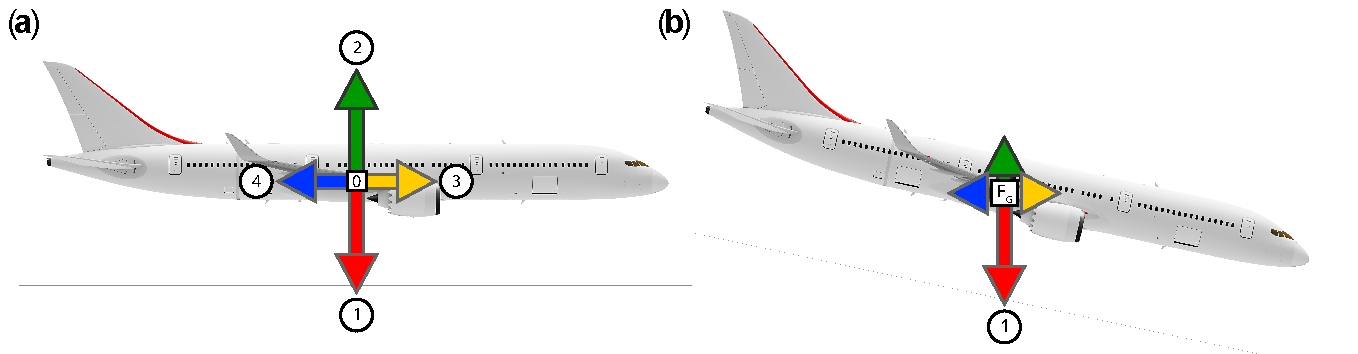
\includegraphics[width=\textwidth]{KraefteFlugzeug.pdf}
\caption[Wirkende Kr�fte am Flugzeug]{Wirkende Kr�fte am Flugzeug. \fa Normaler Flug bei konstanter H�he. \fb W�hrend der $0\,g$ Phase des Parabelflugs} 
\label{abb:bew_Parabelflug01}
\end{figure}
Um den Auftrieb auf Null zu bringen, erzeugt man durch das H�henruder des Flugzeugs einen negativen Anstellwinkel, der Schub kompensiert gerade noch den Luftwiderstand. 
Dynamisch sieht der Parabelflug wie folgt aus (\figref{bew_Parabelflug02}): 
Flugzeug fliegt mit $\SI{825}{\km\per\hour}$ in einer H�he von $\SI{6100}{\metre}$. Es beginnt dann einen Steigflug unter einem Winkel von ca. $45\degree$ f�r ca. $\SI{20}{\second}$ auf ca. $\SI{7600}{\metre}$ mit einer Beschleunigung von ca. $\SI{1.8}{\g}$. Nun wird das Flugzeug in den freien Fall (bzw. noch am Anfang \glqq Wurf\grqq{}) gebracht. Wir haben also eine Wurfparabel mit $v_0=$, $\alpha = 45\degree$, $h_0 = \SI{7600}{\metre}$. 
Die Scheitelh�he dieses Wurfes wird bei $h_\text{max} = \SI{8500}{\metre}$ mit einer verbleibenden Geschwindigkeit $v_\text{Top} = \sqrt{{v_\text{x}}^2+{v_\text{z}}^2}$ von $\SI{370}{\km\per\hour}$ erreicht, danach beginnt der freie Fall mit $\alpha=-45\degree$ f�r ca. $\SI{20}{\second}$ und bei einer H�he von $\SI{7600}{\metre}$ wird das Flugzeug \glqq angefangen\grqq{} um die normale Fluglage und Fluggeschwindigkeit wieder zu erreichen.
\begin{figure}[H]
\includegraphics[width=\textwidth]{Parabelflug.pdf}
\caption[Ablauf eines Parabelfluges]{Ablauf eines Parabelfluges} 
\label{abb:bew_Parabelflug02}
\end{figure}
\end {sol} 
%\href{PhysikUncut_Part1.pdf#prb:bew_Parabelflug}{\textcolor{blue} {$\rightarrow$ zur \probref{bew_Parabelflug}.}}\\
\textcolor{blue} {$\rightarrow$ zur} \probref{bew_Parabelflug}.\\
\noindent\rule[1ex]{\textwidth}{0.5pt}  \newpage


%%%-----------------------------------------------------------------------------------------------------------
%%%-----------------------------------------------------------------------------------------------------------


\subsection{�bungen zu beschleunigten Bezugssystemen}

%-----------------------------------------------------------------------------------------------------------
\hypertarget{lsg:bew_AbplattungPlaneten}{}
\begin{sol}{prob:bew_AbplattungPlaneten}\label{lsg:bew_AbplattungPlaneten}%�bung17
\textbf{Abplattung der Planeten} \\  \\
Der Einfachheit halber lassen wir die Striche f�r das System $\vec{\Sigma}'$ weg.
Wir bleiben ja ausschlie�lich im mitbewegten System. Au�erdem schreiben wir der K�rze wegen f�r die Umdrehungsfrequenz der Erde $\omega$ einfach $\omega$, analog f�r die Masse der Erde $M_\text{E}$ einfach $M$ und $R_\text{E}$ einfach $R$ f�r den mittleren Erdradius, sowie $g_0= GM/R^2$ f�r die mittlere Schwerebeschleunigung. Die Beziehungen sind dann auch direkt f�r andere Planeten anwendbar.

\begin{subprobs}
%--------------------------Aufgabenteil 1
%\subprob{�nderung der Schwerebeschleunigung durch die Zentrifugalkraft \\ -- Sph�rische Erde}
\subprob{�nderung der Schwerebeschleunigung durch die Zentrifugalkraft - Modell 0}\\
	\textbf{\textit{Modell 0: }} In diesem Modell wird die Erde (der Planet) als Kugel angenommen (quasi als ein starrer nicht verformbarer K�rper). Durch die Wirkung der Zentrifugalkraft kommt es aber zu einer Abweichung der Lotlinie, \dh der Richtung der Schwerebeschleunigung.\\
	Nach \figref{bew_Rot_Erde5} und Gleichung \eqref{eq:bew_effektives_g} gilt mit $\varphi$ als geographische Breite $g_\text{eff} = g_0 - R\,{\omega}^2\cos^2\varphi$
	und
	\begin{align}
		g'=& \sqrt{{g_\text{eff}^2+{b'_{\text{II}}}^2}} = \sqrt{{g_0}^2-2g_0\, R \,\omega^2\cos^2\varphi + {R}^2\,\omega^4\,\cos^4\varphi + {R}^2\,\omega^4\,\sin^2\varphi\,\cos^2\varphi} \nonumber \\
		=& g_0\sqrt{1+\frac{{R}^2\,\omega^4\,\cos^2\varphi}{g_0^2}\,\bigg[\cos^2\varphi+\sin^2\varphi-2\frac{g_0}{R \omega^2}\bigg]} 
		= g_0\sqrt{1+\frac{{R}^2\,\omega^4\,\cos^2\varphi}{g_0^2}\,\bigg[1-\frac{2g_0}{R\,\omega^2}\bigg]} \,. 
		\label{eq:bew_lsgAbplattung_a1}
	\end{align} 
Die Maximalwerte werden jeweils bei $\varphi = 90\degree$ (am Pol) und die Minimalwerte bei $\varphi = 0\degree$ (am �quator) erreicht, wie man unschwer an der Gleichung erkennt.\\
Interessant ist aber noch die Frage, wann die Abweichung zwischen $\vec{g_{eff}}$ und $\vec{g'}$ maximal wird.
Dies ist gleichbedeutend mit der Suche nach dem Maximum von $\tan\alpha = b'_\text{II} / g_\text{eff}$.
Wie man durch Differenzieren findet (siehe Nebenrechnung) ergibt sich
\begin{align*}
\alpha_\text{max} &=\arcsin\lk\frac{\frac{1}{2} R\,\omega^2}{g_0-\frac{1}{2} R\,\omega^2}\rk 
\qquad \text{bei} \qquad
\varphi_\text{max} =\arctan\sqrt{1-\frac{R\,\omega^2}{g_0}} \,.
\end{align*}
F�r $R\, \omega^2 \ll g_0$ ergibt sich $\varphi_\text{max} \approx 45\degree$ und $\alpha_\text{max}\approx R \omega^2 / {2g_0} = 0.0989\degree$ (siehe \mscr~\mlbewref{AbplattungPlaneten.m}). Wir werden sehen, dass diese Abweichung der Lotlinie nicht ganz korrekt ist, denn wir haben ja die Abplattung der Erde in unserem Modell vernachl�ssigt. 
\begin{nebenrechnung}{Nebenrechnung:}
		\begin{align*}
		    \tan \alpha = \frac{b'_\text{II}}{g_\text{eff}} = \frac{R{\omega}^2\cos\varphi\sin\varphi}{g_0 - R{\omega}^2\cos^2\varphi} ~\rightarrow~
				\frac{\d}{\d\varphi}\tan\alpha(\varphi) = \cos^2(\varphi)(g_0-R\omega^2\sin^2(\varphi))-g_0\,\sin^2\varphi-R\omega^2\cos^4(\varphi) = 0 \\
				\rightarrow~g_0-R\omega^2\sin^2\varphi =g_0\tan^2\varphi+R\omega^2\cos^2\varphi ~\rightarrow ~ g_0(1-\tan^2\varphi) = R\omega^2 ~\rightarrow ~\tan\varphi_\text{max} =\sqrt{1-\frac{R\omega^2}{g_0}}\,. % ~~ \text{mit} ~~ \varphi_\text{max} = \arctan\sqrt{1-\frac{R\,\omega^2}{g_0}} \, .
		\end{align*}
\end{nebenrechnung}

\newpage
	%--------------------------Aufgabenteil 2
	\subprob{Berechnung der Abplattung der Erde}
In dieser Teilaufgabe wollen wir die Abplattung der Erde aus den bekannten Messwerten $\omega, M, g_0$ und dem �quatorradius $R_\text{A}$ berechnen. Wir werden dazu verschiedene Modelle betrachten.
	\begin{enumerate} [a) ] 
		\item \textbf{ Modell 1 }\\
	
	  Im \textit{Modell 1} wird die Oberfl�che der Erde als \textit{�quipotentialfl�che}\index{�quipotentialfl�che} angenommen. Um eine stabile Oberfl�che zu erhalten, muss die potentielle Energie, die sich aus der Summe der Gravita\-tionskr�fte und der Zentrifugalkr�fte ergibt, entlang der Oberfl�che konstant sein. Andernfalls w�rde sich ja die als verformbar angenommene Oberfl�che ausgleichen wollen. Die Oberfl�che stellt sich dann senkrecht zu $\vec{F_\text{Z}} + \vec{F}_\text{G}$ \bzw zu $\vec{g}'$ (\figref{bew_lsg_Erdrot1}) ein.\footnote{Das ist �quivalent der Richtung der sogenannten \textit{Lotlinie}\index{Lotlinie} (engl. \textit{plumb line}), die man sich aus der Richtung eines aufgeh�ngten Bleigewichts im Unterschied zu einer in den Erdmittelpunkt gerichteten Linie vorstellen und entsprechend berechnen kann (siehe dazu Betrachtung im Aufgabenteil 1 und \cite{Mohazzabi2000}).}
		Die Tangente an einem Oberfl�chenpunkt ist dann logischerweise ebenfalls senkrecht zur Summe aus Gravitations- und Zentrifugalkraft.\\
%Der so definierte K�rper ist kein Rotationsellipsoid. 
	
		Wir betrachten einen Massepunkt $m$ auf der Erdoberfl�che. Wir nehmen zun�chst eine Geometrie eines Rotationsellipsoids an, in der Erwartung, dass die Form des sich einstellenden K�rpers einem solchen entspricht (\figref{bew_lsg_Erdrot2}). Dann k�nnen wir schreiben\footnote{Man muss hinsichtlich der Bezeichnung geographische Breite \index{Geographische Breite, engl. \textit{latitude}} $\varphi$ und geozentrische Breite \index{Geozentrische Breite, engl. \textit{declination}} $\psi$ aufpassen, in der Literatur wird das nicht immer einheitlich gehandhabt. Vgl.\ dazu auch \figref{bew_lsg_Erdrot1} und Kapitel 3 im Band II dieser Reihe. F�r die Kugel gilt nat�rlich $\varphi = \psi$.}: 
		\begin{align}
			x^2+z^2=r^2(\varphi)\,.
		\end{align}
		F�r die Zentrifugalkraft gilt:
		\begin{align}
			\vec{F}_\text{Z} = m \, \omega^2 \left(		\begin{array}{c}		x \\		0 \\		\end{array}		\right) \,. \label{eq:bew_lsgAbplattung01}
		\end{align}
		F�r die Gravitationskraft setzen wir an:
		\begin{align}
			\vec{F}_\text{G} = - \frac{G  M  m}{r^3}\left(		\begin{array}{c}		x \\		z \\		\end{array}		\right)\,. \label{eq:bew_lsgAbplattung02}
		\end{align}
		Das Modell nimmt hier an, dass die Gravitationskraft in Richtung des Mittelpunktes zeigt.
Das ist inkorrekt, da wir ja in Teilaufgabe 1 und in \kap{bew_Coriolis-Kraft} gesehen haben, dass die Gravitationskraft nicht mehr in Richtung Erdmitte zeigt.
		Wir wollen zun�chst dennoch mit dieser N�herung fortfahren, um zu sehen, wie weit wir kommen und wie weit das Ergebnis von der Realit�t abweicht.\\
    Ein Tangentenvektor an die Oberfl�che ist \zb gegeben durch (auch das ist nicht ganz korrekt nach oben Gesagtem):
		\begin{align*}
		\vec{t} = \left( 	\begin{array}{c} 		1 \\		z'	\end{array}		\right) =	\left(		\begin{array}{c}		1 \\ 		\D z / \D x  		\end{array}		\right)\,.
		\end{align*}
		F�r eine stabile Oberfl�che muss wie gesagt gelten:
		\begin{align}
		(\vec{F}_\text{G}+\vec{F}_\text{Z})\cdot \vec{t}= 0 \,, \label{eq:bew_lsgAbplattung03}
		\end{align}
		woraus 
		\begin{align}
		-\frac{G M}{(x^2+z^2)^{\frac{3}{2}}}\,(x+z\, z') + \omega^2 \,x  = 0\, \label{eq:bew_lsgAbplattung04}
		\end{align}
		folgt. Unter den gemachten (N�herungs-)Annahmen haben wir mit Gl. \eqref{eq:bew_lsgAbplattung04} eine Differentialgleichung $z'(x,x',z)$ erhalten, die die Oberfl�chenform z(x) der Erde beschreibt.\\
		Mit dem Ansatz $\hat q=x^2+z^2$ kann diese DGL in 
		\[-\frac{1}{2}G\, M \,\hat q'\,\hat q^{-\frac{3}{2}}+\omega^2 \,x = 0 \]
		�berf�hrt werden, die sofort integriert werden kann
		\begin{align}
		\frac{G \,M}{\sqrt{x^2+z^2}}+\frac{1}{2}\omega^2 \,x^2 = C = \frac{G \,M}{R_\text{P}} \,, \label{eq:bew_lsgAbplattung05}
		\end{align}
		 was man leicht durch Differenzieren nachrechnet. Hierbei haben wir die Integrationskonstante $C$ sinnvollerweise so gew�hlt, dass wir bei $x= 0$ f�r $z$ den Polradius $z = R_\text{P}$ erhalten.
    F�r die Oberfl�chenform $z(x)$ erhalten wir schlie�lich:
		\begin{align} 
		z(x)= R_\text{P} \sqrt{\lk \frac{\omega^2 \,R_\text{P}}{2 G \,M}\, x^2 - 1 \rk^{-2} -\frac{x^2}{R_\text{P}^2}} \,. \label{eq:bew_lsgAbplattung06}
		\end{align}
Offensichtlich ist \eqref{eq:bew_lsgAbplattung06} nur n�herungsweise eine Ellipsengleichung, die man eigentlich als L�sung erwartet h�tte. In \mscr{}~\mlbewref{AbplattungPlaneten.m} haben wir die Oberfl�chenform nach Gl. \eqref{eq:bew_lsgAbplattung06} und auch die Abweichung zu einer Ellipse numerisch berechnet.

\begin{figure}[H]
\includegraphics[scale=1]{Lsg_Erdrot1.pdf}
\caption[Richtung der Gravitationskraft]{Richtung der Gravitationskraft bei kugelf�rmigen und abgeplatteten Planeten.
Eingezeichnet sind die Gravitationskraft $\vec{F}_\text{G}$ und die Zentrifugalkraft $\vec{F}_\text{Z}$, sowie die aus beiden resultierende Kraft.
Im Fall des abgeplatteten Planeten ist im Bild die N�herungsannahme enthalten, dass die wesentliche Masse des Planeten in der N�he des Kerns konzentriert ist.
In der Realit�t w�rde aber die Richtung von $\vec{F}_\text{G}$ je nach Masseverteilung nicht unbedingt zum Erdmittelpunkt zeigen (gestrichelt gezeichnet), was zu einer weiteren Verkippung der Tangente f�hrt.} \label{abb:bew_lsg_Erdrot1}
\end{figure}

\begin{figure}
\centering
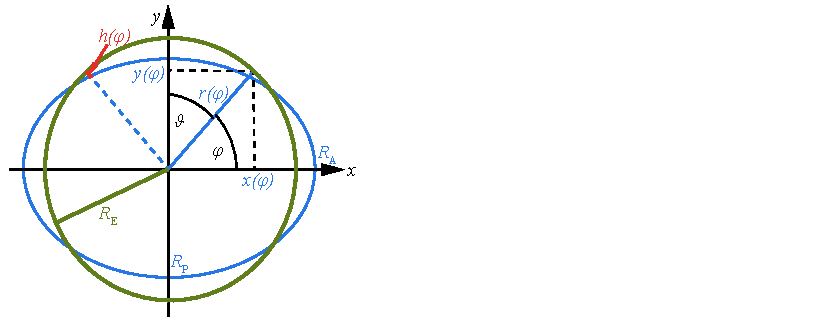
\includegraphics[scale=1]{Lsg_Erdrot2.pdf}
\caption{Geometrie der Abplattung} \label{abb:bew_lsg_Erdrot2}
\end{figure}

Wir wollen aus \eqref{eq:bew_lsgAbplattung05} nun das Verh�ltnis von Pol- zu �quatorradius ausrechnen, indem wir $z(R_\text{A})=0$ und $x=R_\text{A}$ setzen.
Wir erhalten dann aus \eqref{eq:bew_lsgAbplattung05}
	\begin{align} 
	1 +\frac{\omega^2}{2 G M}\, {R_\text{A}}^3 = \frac{R_\text{A}}{R_\text{P}} = \kappa \,. \label{eq:bew_lsgAbplattung07}
	\end{align}
	woraus der Polradius
	\begin{align} 
	R_\text{P} = \frac{R_\text{A}}{1+\frac{\omega^2}{2 G M} \, {R_\text{A}}^3} \label{eq:bew_lsgAbplattung08}
	\end{align}
folgt.
Die sogenannte \textit{Abplattung}\index{Abplattung} $f$ ist definiert als 
	\begin{align} 
	f = \frac{R_\text{A}-R_\text{P}}{R_\text{A}} = 1-\frac{R_\text{P}}{R_\text{A}} = 1-\frac{1}{\kappa} \,. \label{eq:bew_lsgAbplattung08a}
	\end{align}
In entsprechender N�herung gilt also f�r unser Modell 1 
	\begin{align}
	f_1 \approx 1- \lk 1-\frac{\omega^2}{2 G\,M}\, {R_\text{A}}^3 \rk  \approx \frac{\omega^2}{2\,G\,M}\, {R_\text{A}}^3 \approx \frac{3\omega^2}{8\pi\,G\,\varrho_\text{E}} \,. \label{eq:bew_lsgAbplattung_Modell01}
	\end{align}
Damit haben wir zun�chst das plausible Ergebnis, dass die Abplattung umso gr��er wird, je gr��er die Rotationsgeschwindigkeit und je kleiner die \anf{mittlere} Dichte wird.
Wenn wir allerdings die tats�chlichen Werte der Erde 
\begin{align*}
{R_\text{A}}^{\text{(exp)}} &= \SI{6378.137}{\km}\,,~M = \SI{5.974e24}{\kg}\,,\\
\omega &= \SI{7.292116e-5} {\per\second}\,,~ G = \SI{6.67384e-11}{\meter\cubed\kg\tothe{-1}\second\tothe{-2}} \,
\end{align*}
einsetzen, erhalten wir f�r den Polradius $R_\text{P}=\SI{6367.120}{\km}$ anstelle der tats�chlich gemessenen ${R_\text{P}}^{\text{(exp)}}=\SI{6356.752}{\km}$, also einen Unterschied der Radien von $\Delta R_1 =\SI{11.0}{\km}$ (im Unterschied zu den tats�chlichen $\Delta R^{\text{(exp)}} = \SI{21.4}{\km}$. Der nach Modell 1 ermittelte Polradius $R_{\text{P},1}$ ist also rund $\SI{10.4}{\km}$ zu gro� und damit erh�lt man mit
	\begin{align*}
		f_1 = 1:579.9  ~\quad \text{anstelle der gemessenen} ~\quad f^{\text{(exp)}} = 1:298.25\,,
	\end{align*}
auch eine deutlich zu geringe Abplattung.\\

%--------------------------Aufgabenteil 2b

\item \textit{\textbf{Modell 2}}\\
	   Wir wollen nun ein anderes Modell verwenden und betrachten dazu \figref{bew_lsg_Erdrot2}. In diesem \textit{Modell 2}
		 wollen wir die (rotierende) Erde als eine homogene Referenzkugel mit Radius $R$, Dichte $\rho_\text{E}$ und Masse $M=4\pi\varrho R^3/3$ plus einer infinitesimal d�nnen Schale mit positiver und negativer Masse auf $r=R$ mit einer Fl�chenmassendichte $\sigma(\theta)$ modellieren. Die d�nne Schicht beschreibt die  Massenumlagerung durch Abplattung und besitzt insgesamt ein \emph{Nullmasse}. Die resultierende Oberfl�che aus Kugel und Schicht sei wiederum eine geforderte �quipotentialfl�che des Gesamtpotentials.\footnote{Im Modell 1 hatten wir die Verformung einen rotierenden K�rpers (mit flexibler, fluider Oberfl�che) berechnet.) Die Gleichung \eqref{eq:bew_lsgAbplattung05} hatten wir als �quipotentialgleichung formuliert, wobei wir dort in guter N�herung das Gravitationspotential durch $-M g_\text{0} h(\varphi)= -M g_\text{0} h(\vartheta)$ ersetzt hatten. Wir k�nnten nat�rlich auch besser nach Aufgabenteil 1 $g_{\text{eff}}$ einsetzen, was die Rechnungen etwas verkompliziert, aber am Ergebnis nichts grunds�tzlich �ndert.} F�r die folgenden Rechnungen werden Grundkenntnisse der Potentialtheorie vorausgesetzt, wie wir sie in Band II und Band IV dieser Reihe im Detail behandeln. \\

Wir schreiben das Gesamtpotential als Summe von Gravitationspotential $U_\text{G}$ und dem Zentrifugalpotential $U_\text{Z}$, \dh $~U_{\text{tot}} = U_\text{G} + U_\text{Z}~$ und es 
gilt $~U_{\text{tot}}(\text{�quator})=U_{\text{tot}}(\text{Pol})~$. 
Mathematisch �quivalent zur Forderung an die �quipotentialfl�che ist die Bedingung, dass im Potential $U_\text{tot}$ auf der Oberfl�che kein
$\theta$-abh�ngiger Anteil verbleiben darf (zumindest bis zur betrachteten Ordnung).

Wir wollen eine kleine Abplattung annehmen ($\varepsilon  \ll 1$) und parametrisieren die Oberfl�che als ($\ell=2$-) Deformation �ber 
\begin{equation}
r_s(\vartheta)=R\lk 1+\varepsilon\,\PL2(\cos\vartheta)\rk \quad \text{worin}~~\PL2(\cos\vartheta)=\frac12(3\cos^2\vartheta-1) ~~\text{und} ~~|\varepsilon|\ll 1\,.
\end{equation}
Damit gilt
\begin{align}
		R_\text{P} &= r_s(\vartheta=0)=R\,(1+\varepsilon) \quad \text{und} \quad R_\text{A} = r_s\,\lk \vartheta=\frac{\pi}{2}\rk = R\,\lk 1-\frac{\varepsilon}{2}\rk\,.
\end{align}
F�r reale Abplattung ist \iA $R_\text{A}>R_\text{P}$, also $\varepsilon<0$. Die geometrische Abplattung $f$
liefert bis zur ersten Ordnung in $\varepsilon$:
\begin{equation}
		f_2=\frac{R_\text{A}-R_\text{P}}{R_\text{A}} =\frac{R\,(1-\varepsilon/2)-R\,(1+\varepsilon)}{R\,(1-\varepsilon/2)} \approx -\frac{3}{2}\varepsilon\,\quad\rightarrow\quad \varepsilon\approx -\frac{2}{3}\,f\,. \label{eq:f_eps}
\end{equation}
Wir berechnen nun das Gravitationspotential der Kugel plus der d�nnen Schale. Auf der Oberfl�che $r=r_s(\vartheta)=R\,(1+\varepsilon\,\PL2)$ entwickeln wir das Potential nach Ordnungen von $\varepsilon$:
\begin{equation}
		U_\text{G,K}(r_s,\vartheta)= -\frac{GM}{R\,\lk 1+\varepsilon\, \PL2(\cos\vartheta)\rk} \approx -\frac{GM}{R}\lk 1-\varepsilon\, \PL2(\cos\vartheta)\rk = -\frac{GM}{R}+\frac{GM}{R}\,\varepsilon\,\PL2(\cos\vartheta)\,.
\end{equation}
Der $\PL2$-Anteil daraus ist
\begin{equation}
		U_{G,K}^{(\ell=2)}(\vartheta)=\frac{GM}{R}\,\varepsilon\,\PL2(\cos\vartheta)\,. \label{eq:U02}
\end{equation}
Die d�nne Schale als Massenumlagerung mit der Gesamtmasse Null stellt als Masseverteilung einen Quadrupol dar. Ihre radiale Oberfl�chenabweichung von der Referenzkugel ist gegeben durch
\begin{equation}
		\delta r(\vartheta)=r_s(\vartheta)-R=R\,\varepsilon\,\PL2(\cos\vartheta)\,
\end{equation}
und ihre Fl�chenmassendichte ist
\begin{equation}
		\sigma(\vartheta)=\rho\,\delta r(\vartheta)=\underbrace{\rho R\,\varepsilon}_{\sigma_2}\,\PL2(\cos\vartheta) = \sigma_2\,\PL2(\cos\vartheta)\,.
\end{equation}
Da $\int \PL2\,\D \Omega=0$ ist, ist die Forderung Gesamtmasse Schale $=0$ erf�llt.
Wir bestimmen f�r die Massenverteilung $\sigma(\vartheta)$  auf der Oberfl�che das Multipolmoment mit $\ell=2$:
\begin{equation}
		M_2=\intsl \sigma(\vartheta)\,R{}^{4}\,\PL2(\cos\vartheta)\,\D\Omega  =\sigma_2\,R{}^4\intsl \PL2{}^2\,\D\Omega\,.
\end{equation}
Unter Ausnutzung der Orthogonalit�t der Legendre-Polynome 
\begin{equation}
		\int \PL\ell{}^2\,\D\Omega=\frac{4\pi}{2\ell+1} \quad\Rightarrow\quad \intsl \PL2{}^2\,\D\Omega=\frac{4\pi}{5}\,,
\end{equation}
folgt:
\begin{equation}
		M_2=R^4 \frac{4\pi}{5}\, \sigma_2\, =\frac{4\pi}{5}\rho \varepsilon\,R{}^5\,.
\end{equation}
Das �u�ere Potential eines reinen Quadrupol-Moments ($\ell=2$) lautet nach der Potentialtheorie (der Subskript S steht f�r Schale)
\begin{equation}
		U_{\text{G,S}}^{(\ell=2)}(R,\vartheta)= -\frac{G}{R{}^3}M_2 =-\frac{G}{R{}^3}\left(\frac{4\pi}{5}\rho \varepsilon\, R{}^5\right)\,\PL2 = -\frac{4\pi G\rho\, R{}^2}{5}\,\varepsilon\,\PL2(\cos\vartheta) 
		= -\frac{3}{5}\frac{GM}{R}\,\varepsilon\,\PL2(\cos\vartheta)\,. \label{eq:Ush2}
\end{equation}
Aus \eqref{eq:U02} und \eqref{eq:Ush2} folgt f�r den gesamter $\PL2$-Anteil des Gravitationspotentials
\begin{equation}
		U_{G}^{(\ell=2)}(\vartheta)(\vartheta)=U_\text{G,K}^{(\ell=2)} + U_\text{G,S}^{(\ell=2)} =\lk 1-\frac{3}{5}\rk \frac{GM}{R}\varepsilon\,\PL2(\cos\vartheta) =\frac{2}{5}\frac{GM}{R}\,\varepsilon\,\PL2(\cos\vartheta)\,.\label{eq:Ug2}
\end{equation}

Nun brauchen wir noch den $\PL2$-Anteil des Zentrifugalpotentials.
Das gesamte Zentrifugalpotential ist
\begin{equation}
		U_\text{Z}(\vartheta)=-\frac12\omega^2 r^2\sin^2\vartheta\,.
\end{equation}
Wir ben�tigen den $\PL2$-Anteil bei $r\approx R$.
Mit
\begin{equation*}
		\sin^2\vartheta = 1-\cos^2\vartheta ~~ \text{\bzw}~ \cos^2\vartheta=\frac{1+2\,\PL2(\cos\vartheta)}{3}~~\text{und}~~	\sin^2\vartheta=\frac{2}{3}\lk 1-\PL2(\cos\vartheta)\rk
\end{equation*} erhalten wir
\begin{equation}
		U_\text{Z}(\vartheta)= -\frac12\omega^2 R{}^2\,\frac{2}{3}\lk 1-\PL2(\cos\vartheta)\rk = -\frac{1}{3}\omega^2 R{}^2 + \frac{1}{3}\omega^2 R{}^2\,\PL2(\cos\vartheta) = -\frac{1}{3}\omega^2 R{}^2 + U_\text{Z}^{(\ell=2)}(\vartheta)\,. \label{eq:Uc2}
\end{equation}
Da die Oberfl�che eine �quipotentialfl�che sein muss, muss der
$\vartheta$-abh�ngige Anteil (also der gesamte Koeffizient von $\PL2$) des Gesamtpotentials
auf der Oberfl�che verschwinden, \dh
\begin{equation}
		U_{G}^{(\ell=2)}(\vartheta) + U_\text{Z}^{(\ell=2)}(\vartheta)=0\,.
\end{equation}
Mit \eqref{eq:Ug2} und \eqref{eq:Uc2} erh�lt man daraus
\begin{equation}
		\frac{2}{5}\frac{GM}{R}\,\varepsilon + \frac{1}{3}\omega^2 R{}^2=0 	\quad\rightarrow\quad \varepsilon = -\frac{5}{6}\frac{\omega^2R{}^3}{GM}\,. \label{eq:eps_result}
\end{equation}
%
Mit \eqref{eq:f_eps} folgt unter den getroffenen Annahmen, \dh homogene Kugel plus infinitesimal d�nne Massenschale und kleiner Abplattung aus der �quipotential-Bedingung in erster Ordnung nach unserem Modell 2 
f�r die Abplattung 
\begin{equation}
		f_2 \approx -\frac{3}{2}\varepsilon = \frac{5}{4}\frac{\omega^2R{}^3}{GM} \approx 1:231.95\,. \label{eq:bew_lsgAbplattung_Modell02}
\end{equation}
Wir haben eine gegen�ber dem Modell 1 (Gl. \eqref{eq:bew_lsgAbplattung_Modell01}) verbesserte L�sung (siehe Tabelle \ref{tab:bew_AbplattungenModelle}), die aber immer noch die Realit�t nicht vollst�ndig korrekt beschreibt. Die Abplattung nach diesem Modell ist um den Faktor 5/2 gr��er als im Modell 1, nun aber um \ca $\SI{6.5}{\km}$ zu gro�.
Die Abweichung liegt darin begr�ndet, dass wir die Erde als homogen angenommen hatten. 
Die Realit�t liegt zwischen dem homogenen Fall (Modell 2) und dem Modell 1, das als Modell eines K�rpers angesehen werden kann, bei dem die wesentliche Masse im Zentrum desselben konzentriert ist (deswegen konnten wir ja auch die Gravitationskraft noch im Wesentlichen in Richtung Erdmittelpunkt zeigend annehmen).\\
Tats�chlich ist die Erde aber mit $f=1/298.25$ kugel�hnlicher als unser Modell 2 hergibt, weil ihr Kern mehr als doppelt so dicht wie der Mantel ist. Dadurch f�llt die Fliehkraft weniger ins Gewicht. Diese gr��ere Dichte des Erdkerns k�nnte besser mit einem Zwei-oder Mehr-Schalen-Modell des Erdinneren ber�cksichtigt werden\footnote{Dieses Modell erkl�rt dann auch das beobachtete Schwerefeld im nahen Weltraum relativ gut. Feinere Erdmodelle der Geophysik unterteilen Kruste, Erdmantel und Erdkern je zweimal, womit man aber bereits an die Grenzen der Berechenbarkeit st��t (siehe auch \probref{bew_traegheitsmomente}).}, wobei man dann, um die Gravitationskraft korrekt zu ber�cksichtigen, �ber alle infinitesimalen Massenelemente der Erde integrieren muss. Alternativ kann man nat�rlich auch die hier f�r $\ell=2$ abgebrochene Reihenentwicklung des Potentials nach Kugelfl�chenfunktionen  mit $\ell = 3,4 \ldots$ fortsetzen. \\

	%---------------------------------Teil2c
\item \textit{\textbf{Modell 3}}\\
	   Wir wollen im \textit{Modell 3} das Modell 2 etwas allgemeiner behandeln, in dem wir den Erdk�rpers nun aus einer Referenzkugel und Schicht (mit Dicke $h(\vartheta)$)) bestehend betrachten.\footnote{Das Modell l�sst sich dann auch leicht auf inhomogene Massenverteilung verallgemeinern, wenn auch die Integration entsprechend schwierig wird.} Wir berechnen wieder die �quipotentialfl�che als Addition der Effekte der Gravitation der Kugel, der Zentrifugalkraft und der Gravitation von der d�nnen Schale. Letzteres stellt die eigentliche Komplexit�t dar, denn wir m�ssen ja das Volumenintegral �ber alle Massenelemente der Schale (oder eines entsprechenden beliebigen Zusatzk�rper) bilden.

Wir wollen zun�chst eine N�herungsform f�r die Dicke der Schicht ableiten. 
F�r die �quipotentialfl�che kann man n�herungsweise herleiten (siehe Gl. \eqref{eq:bew_effektives_g} in \kap{bew_Coriolis-Kraft}:
\begin{align}
	g_0 h(\vartheta) + \frac{\omega^2}{2}\, R^2 \, \sin^2\vartheta = \text{const} \quad \rightarrow \quad \hat C =  h(\vartheta)-\frac{\omega^2\, {R}^2 \,\sin^2\vartheta}{2 g_0}\,. \label{eq:bew_lsgAbplattung09} 
\end{align}
Um $\hat C$ zu bestimmen, machen wir die plausible Annahme, dass das Volumen des Rotationsellipsoids gleich dem der unverformten Kugel ist, d.h. es findet zwar eine Verformung, aber keine Kompression statt (man denke an eine Wasseroberfl�che oder ein fl�ssiges Plasma). Diese Bedingung ist gleichbedeutend mit 
\begin{align*}
	I &= \intsl\limits_{0}^{2\pi}\int\limits_{0}^{\pi}h(\vartheta)\,\sin\vartheta \,\,\D \varphi\, \D\vartheta = 2\pi \intsl\limits_{0}^{\pi}\lek\hat C +\underbrace{\lk\frac{\omega^2\,{R}^2}{2 g_\text{0}}\rk}_{\substack{\hat D}} \lk1- \cos^2\vartheta\rk\rek  \sin\vartheta \, \D \vartheta\,\nonumber \\
	 &=2\pi \,\lek-\hat C  \cos\vartheta - \hat D  \cos\vartheta + \hat D \frac{ \cos^3\vartheta}{3}\rek^{0}_{\pi} = 2\pi \,\lek\underbrace{+ 2\hat C + 2 \hat D - \frac{2}{3} \hat D}_{= 0}\rek \stackrel{!}{=} 0 \,. \nonumber
\end{align*}
Daraus folgt mit \eqref{eq:bew_lsgAbplattung09}
\begin{align}
	\hat C = -\frac{2}{3}\hat D = -\frac{\omega^2\,{R}^2}{3 g_\text{0}}  ~~\rightarrow~~h(\vartheta) = \frac{{R}^2\,\omega^2}{6 g_\text{0}}\,(3 \sin^2\vartheta-2)	\,.
\end{align}
Wenn man damit die Abplattung $f$ �ber $R_\text{A} = R + h(\vartheta=\pi/2), R_\text{P} = R + h(\vartheta=0)$ berechnet, ergibt sich wie erwartet der gleiche Wert wie f�r Modell 1 in Aufgabenteil 2a, n�mlich $f= \omega^2\,{R}^3/(2GM)$ (hier nur $R$ statt $R_\text{A}$), was aber keinen gro�en Unterschied macht.)\\
Wir wollen jetzt dieses H�henprofil $h(\vartheta)$ als Startwert verwenden und m�ssen zur Berechnung der Gravitationskraft der Schicht das Volumenintegral �ber alle Massenelement bilden. F�r jedes Massenelement gilt:
	\begin{align*}
			\D M = \varrho \,\D V = \varrho\,h(\vartheta) \,\D A = \varrho\,\beta(\gamma)\,(3 \sin^2\vartheta-2)\,R^2 \,\sin\vartheta\,\D \lambda \,\D \vartheta\,. 
	\end{align*}
Hier haben wir mit Gl \eqref{eq:bew_lsgAbplattung09} das H�henprofil in der $\vartheta$-Abh�ngigkeit unver�ndert gelassen, aber einen Korrekturfaktor  $\gamma>1$ eingef�gt. Dieser soll die aus den Richtungsabweichungen der Gravitationskraft resultierenden Effekte im Potential abbilden:
	\begin{align}
			h(\vartheta)=\beta(\gamma) \,(3 \sin^2\vartheta-2) ~~~\text{mit}~~~ \beta(\gamma)\,=\,\gamma\,\frac{R{}^2\,\omega^2}{6g_0} \,. \label{eq:ansatz_form}
	\end{align}
Aus der geometrischen Betrachtung von \figref{bew_lsg_Erdrot2} kann man ableiten, dass sich die Abst�nde f�r die Potentialberechnung $\text{Nordpol-Massepunkt auf der Oberfl�che}$ nach $d_1 = R\sqrt{2(1- \cos\vartheta)}$ \bzw $\text{�quator-Massepunkt}$ nach  $d_2 = R\sqrt{2(1- \sin\vartheta \,\cos\lambda)}$ berechnen. ($\lambda$ ist hier die Integrationsvariable L�ngengrad.)
Als spezielle Forderung einer �quipotentialfl�che fordern wir jetzt, dass das Gesamtpotential am �quator und den Polen gleich ist, was gleichbedeutend ist mit 
	\begin{align*}
   U_\text{tot}(\vartheta=0) &= (-2)\,g_0 \,\beta  + 0 - \intsl\limits_{0}^{\pi}\int\limits_{0}^{2\pi}\frac{G\,\varrho(\vartheta,\lambda)\,\beta\,(3 \sin^2\vartheta-2)}{R\sqrt{2(1- \cos\vartheta)}}{R}^2 \sin\vartheta\: \D\vartheta \,\D\lambda ~\\
	= U_\text{tot}(\vartheta=90\degree) & = (1)\,g_0 \,\beta  -\frac{m}{2} \omega^2 \ - \intsl\limits_{0}^{\pi}\int\limits_{0}^{2\pi}\frac{G\varrho(\vartheta,\lambda)\beta(3 \sin^2\vartheta-2)}{R\sqrt{2(1- \sin\vartheta\, \cos\lambda)}}{R}^2 \sin\vartheta\: \D\vartheta \,\D\lambda \,. 
\end{align*}
Hier nehmen wir nun eine \textit{homogene} Massenverteilung an, man k�nnte aber auch numerisch weiter mit $\varrho(\vartheta,\lambda)$ rechnen, um eventuell (bekannte) inhomogene Verteilungen mitzunehmen. Wir erhalten damit:
\begin{align}
	\gamma -1 = \gamma\intsl\limits_{0}^{\pi}\intsl\limits_{0}^{2\pi}\lek \frac{{R}^2}{4\pi R}(3 \sin^2\vartheta-2) \sin\vartheta\, \rek \, \lek\frac{1}{R\sqrt{2(1- \sin\vartheta \,\cos\lambda)}}-\frac{1}{R_\text{E}\sqrt{2(1- \cos\vartheta)}} \rek \,\D\lambda\,\D\vartheta\,, \label{eq:bew_gamma_abplattung}
\end{align}
woraus sich der Korrekturfaktor $\gamma$ �ber 
\begin{align}
	\gamma=1/(1-\mathcal{I})~\text{mit}~
	\mathcal{I}= \int\limits_{0}^{\pi}\int\limits_{0}^{2\pi}\frac{3 \sin^2\vartheta-2}{4\sqrt{2}\pi}\,\lk\frac{1}{\sqrt{1- \sin\vartheta \,\cos\lambda}}-\frac{1}{\sqrt{1- \cos\vartheta}}\rk \:\D\lambda\,\sin\vartheta \D\vartheta\,  \label{eq:bew_lsgAbplattung11}
\end{align}
berechnet. Dieses Integral k�nnen wir numerisch l�sen und erhalten $\gamma=5/2$ und damit $\Delta \text{R}=\SI{27.5}{\kilo\metre}$, also das gleiche Ergebnis wie in Teilaufgabe 2b) n�mlich im Vergleich zur Realit�t $\SI{21.4}{\kilo\metre}$ eine zu starke Abplattung von $\SI{6.1}{\kilo\metre}$. Das war auch zu erwarten, weil die Annahme einer homogenen Massenverteilung, wie wir sie im Schritt zu Gl.\eqref{eq:bew_gamma_abplattung} verwendet haben, wie wir gesehen haben ebenfalls nicht ganz korrekt ist.\\
Die Form nach dem Modell der so abgeplatteten Erde ist auch kein Rotationsellipsoid, wir hatten die Form ja mittels Gl. \eqref{eq:ansatz_form} in die Berechnung ``hinein gesteckt''. 

Man kann aber zeigen, dass man auch ohne eine Formannahme (wie in Modell 2 oder 3) f�r eine \textbf{homogene} Massenverteilung, das Problem allein aus der �quipotentialforderung f�r die Oberfl�che exakt l�sen kann\footnote{Siehe Zusatz�bung \probref{bew_abplattung_exakt} und \cite{Ledersteger1960}.}
 und dass dann die Form auch tats�chlich ein Rotationsellipsoid mit
\begin{align}
\frac{x^2}{R_\text{A}{}^2} + \frac{z^2}{R_\text{P}{}^2} = 1 ~~ \text~~ \eta = R_\text{A}/R_\text{P} = \frac{1}{\kappa}> 1
\end{align}
ist, wobei $\eta$ folgende Bedingung erf�llen muss:
\begin{align}
	(\eta^2+2)(\eta^2-1)^{-\frac{3}{2}}\arctan \sqrt{\eta^2-1}-\frac{3}{\eta^2-1} = \frac{{\omega}^2}{2 \pi \,G \,\varrho}=\frac{2\, R^3}{3\,G \,M}\,. \label{eq:bew_lsgAbplattung12}
\end{align}
Diese Gleichung l�sst sich numerisch l�sen und man findet mit $\varrho$ als mittlere Dichte der Erde die L�sung f�r das allgemeine Modell 3
	\[	\eta_3 = 1/\kappa_3 \approx 1.0043297 \,,\]
woraus eine geometrische Abplattung 
\begin{align}
f_3 = \frac{R_\text{A}-R_\text{P}}{R_\text{A}} \approx 1 - \eta \approx 1:230  \label{eq:bew_lsgAbplattung13}
\end{align}
folgt, was f�r die Erde nahe am Modell 2 liegt.\\

\textbf{\textit{Wissenschaftshistorischer Hinweis:}}\\
Die Bestimmung der Abplattung der Erde ist auch wissenschaftshistorisch au�erordentlich interessant, galt sie doch als eine der ersten Best�tigungen der Newtonschen Mechanik. So wurden 1733 und 1735 erste internationale (!) wissenschaftliche Expeditionen nach Equador und Lappland ausgesandt, um die Abplattung geod�tisch zu bestimmen. Diese Expeditionen waren die ersten gro�en \textit{Big Science} Projekte, noch vor der den gro�en Expeditionen zur Beobachtung des Venustransits und der Bestimmung der astronomischen Einheit in den Jahren 1761 und 1769, die wir in der Astrodynamik im Band II, Kapitel 3 behandeln werden. Ihr Budget entsprach damals ca. $0.1\%$ des franz�sischen Staatshaushalts. Wir empfehlen \cite {Greenstein2022} und die dort zitierte Literatur.

\end{enumerate}

	%--------------------------Aufgabenteil 3
\newpage
\subprob{Vergleich mit anderen Planeten}

Mit den L�sungen aus dem vorherigen Aufgabenteil k�nnen wir nun auch Absch�tzungen f�r die Gas\-planeten unseres Sonnensystems machen.
Wir benutzen Formel \eqref{eq:bew_lsgAbplattung08} f�r das Modell 1 des konzentrierten Kerns, welches die Differenz $\Delta R_1$ zwischen �quator- und Polradius ergibt, Formel \eqref{eq:bew_lsgAbplattung08} f�r das Modell 2 einer homogenen Massenverteilung (N�herung der Potentialtheorie mit $\ell=2$), woraus sich die Differenz $\Delta R_2$ ergibt, sowie Formeln \eqref{eq:bew_lsgAbplattung12} und \eqref{eq:bew_lsgAbplattung13} f�r die exakte Berechnung eines Rotationsk�rpers homogener Dichte. Wir vergleichen unsere Berechnungen mit den bekannten experimentellen Werten $f^{(\text{exp})}$ und $R^{(\text{exp})}$. \\

\begin{table}
\centering
    \hspace*{0.2cm}
    \begin{tabular}{L{1.25 cm}L{1.25cm}L{1.25cm}L{1.25cm}L{1.25cm}R{1.0cm}R{1.5cm}R{1.5cm}R{1.5cm}R{1.5cm}}
    Planet 	& $f_1$ & $f_2$ & $f_3$ & $f^{(\text{exp})}$ & $\gamma$ & $\Delta R_1$ & $\Delta R_2$ & $\Delta R_3$ & $\Delta R^{(\text{exp})}$ \\
    \noalign{\smallskip} \hline \noalign{\smallskip}
    Erde    & 579.88 & 231.95  &231.74  & 298.25 &  2.498 & \SI{11.0}{\kilo\metre} &  \SI{27.6}{\kilo\metre} &\SI{27.6}{\kilo\metre} &  \SI{21.4}{\kilo\metre} \\
    \noalign{\smallskip} 
    Jupiter & 23.76  & 9.10  & 9.48    & 15.41   &  2.684 & \SI{3141}{\kilo\metre} &  \SI{7852}{\kilo\metre}  &  \SI{7540}{\kilo\metre}  &\SI{4638}{\kilo\metre} \\
    Saturn  & 14.02  & 5.21  & 5.49    & 10.21   &  2.437 & \SI{4628}{\kilo\metre} &  \SI{11569}{\kilo\metre} &  \SI{10985}{\kilo\metre} &\SI{5904}{\kilo\metre} \\
    Uranus  & 66.84  & 26.34 & 26.74   & 43.62   &  2.462 & \SI{ 388}{\kilo\metre} &  \SI{970}{\kilo\metre}   &  \SI{ 956}{\kilo\metre}  &\SI{ 586}{\kilo\metre} \\
    Neptun  & 77.59  & 30.63 & 30.95   & 58.54   &  2.475 & \SI{ 323}{\kilo\metre} &  \SI{808}{\kilo\metre}   &  \SI{ 800}{\kilo\metre}  &\SI{ 423}{\kilo\metre} \\ 
    \noalign{\smallskip} \hline \noalign{\smallskip}
\end{tabular} 
    \hspace*{0cm}
		\caption[Vergleich der Ergebnisse der Abplattungsberechnungen f�r verschiedene Modelle und Vergleich zu den tats�chlichen Werten.]{Vergleich der Ergebnisse der Abplattungsberechnungen f�r verschiedene Modelle und Vergleich zu den tats�chlichen Werten. F�r die Erkl�rung der einzelnen berechneten Gr��en siehe Text. berechnet mit \mscr{}~\mlbewref{Abplattung.m}.}\label{tab:bew_AbplattungenModelle}
\end{table}

Man erkennt, dass auch bei den Gasplaneten der experimentelle Wert zwischen den Werten der beiden Modelle 1 und 2 liegt, wobei er im Gegensatz zur Erde deutlich dichter am Modell 1 des hochkonzentrierten Kerns liegt, was bei den Gasplaneten auch zu erwarten war. Saturn ist der am st�rksten abgeplattete Planet im Sonnensystem, w�hrend die Erde fast kugelf�rmig im Vergleich zu den Gasriesen ist. Man erkennt im Fall der Erde noch die relativ gute �bereinstimmung der Rechnung nach der Potentialtheorie (Modell 2) mit der exakten Berechnung f�r den Fall homogener Dichte (Modell 3), w�hrend bei den Gasriesen auf Grund von Dichte und Rotationsfrequenz gr��ere Abweichungen zu erkennen sind.

\end{subprobs}

\end{sol} 

%\href{PhysikUncut_Part1.pdf#prb:bew_AbplattungPlaneten}{\textcolor{blue} {$\rightarrow$ zur \probref{bew_AbplattungPlaneten}.}}\\
\textcolor{blue} {$\rightarrow$ zur} \probref{bew_AbplattungPlaneten}.\\
\noindent\rule[1ex]{\textwidth}{0.5pt}  \newpage


%-----------------------------------------------------------------------------------------------------------
\hypertarget{lsg:bew_Coriolis_I}{}
\begin{sol}{prob:bew_Coriolis_I}\label{lsg:bew_Coriolis_I}%�bung18
\textbf{Coriolis-Kraft I -- Ballistik}
\begin{subprobs}
\subprob{Exakte L�sung Freier Fall}
	Die Bewegungsgleichungen folgen aus \eqref{eq:bew_BGL_Erdrotation_Ko}:\:
	\begin{align}
	\ddot{x}(t) &= + 2\omega \sin \varphi \:\dot{y} \nonumber \\
	\ddot{y}(t) &= - 2\omega \sin \varphi \:\dot{x} - 2\omega \cos \varphi \:\dot{z} \nonumber \\
	\ddot{z}(t) &= + 2\omega \cos \varphi \:\dot{y} - g \,. \label{eq:lsg_BallistikCor1_1}
	\end{align}
	Einmalige Integration ergibt:
	\begin{align}
	\dot{x}(t) &= + 2\omega \sin \varphi \:y \nonumber \\
	\dot{y}(t) &= - 2\omega \sin \varphi \:x - 2\omega \cos \varphi \:z \nonumber \\
	\dot{z}(t) &= + 2\omega \cos \varphi \:y - g \,t\,. \label{eq:lsg_BallistikCor1_2}
	\end{align}
	Wir setzen $\dot{x}(t)$ und $\dot{z}(t)$ in die Gleichung f�r $\dot{y}(t)$ ein und erhalten die DGL
	\begin{align}
		\ddot{y} + 4\omega ^2 y = 2 \omega \,g \,\cos \varphi \:t \,,\label{eq:lsg_BallistikCor1_3}
	\end{align}
	deren L�sung durch
	\begin{align*}
		y(t) =  A\,\sin(2\omega\,t) + B\,\cos(2\omega\,t) + \frac{g\,\cos \varphi}{2 \omega} \,t \, , 
	\end{align*}
	gegeben ist. 
	Mit den Anfangsbedingungen $x(0) = y(0) = 0,~ \dot{x}(0) = \dot{y}(0) = \dot{z}(0) = 0$ und $z(0)= h$ folgt sofort $B=0$ und $A = -(g \cos\varphi)/(4 \omega^2)$.
        Die L�sung f�r die Ost-West-Richtung $y$ lautet also
	\begin{align}
		y(t) =  \frac{g \cos\varphi}{2 \omega} \lk t - \frac{\sin(2\omega\,t)}{2\omega} \rk \,.\label{eq:lsg_BallistikCor1_4}
	\end{align}
	Wir setzen nun $y(t)$ in die Gleichungen f�r $\dot{x}(t)$ und $\dot{z}(t)$ ein, integrieren und erhalten daraus mit den Anfangsbedingungen f�r die S�d-Nord-Richtung $x$
	\begin{align}
		x(t) =  g \sin\varphi \,\cos\varphi \,\lk \frac{t^2}{2} - \frac{1- \cos(2\omega\,t)}{4\omega^2} \rk \,,\label{eq:lsg_BallistikCor1_5}
	\end{align}
	\bzw f�r die H�he $z$
	\begin{align}
		z(t) = h - \frac{g \,t^2}{2} + g \cos^2\varphi \,\lk \frac{t^2}{2} - \frac{1-\cos(2\omega\,t)}{4\omega^2} \rk \,.\label{eq:lsg_BallistikCor1_6}
	\end{align}
	Damit haben wir das Problem exakt gel�st.
        F�r $\omega\,t \ll 1$ kann man die L�sung entwickeln
	\begin{align}
	x(t) &=  -\frac{g \sin\varphi \,\cos\varphi}{6} \,t^2 \, \lk\omega\,t\rk^2\,\nonumber \\
	y(t) &=   \frac{g \cos\varphi}{3} \,t^2 \,\lk\omega\,t\rk^2 \,.\nonumber \\
	z(t) &= h - \frac{g\, t^2}{2} + \frac{g}{6}\, \cos^2\varphi\,\, t^2 \,\lk\omega\,t\rk^2 \,.\label{eq:lsg_BallistikCor1_7}
	\end{align}
	F�r $(\omega\,t)^2 \approx 0$ geht dies in die N�herungsl�sung \eqref{eq:bew_BGL_Erdrotation_Lsg1} �ber. 
	Im \mscr~\mlbewref{BallistikCoriolis01.m} haben wir die L�sungen verglichen und auch den Fall eines sich sehr schnell drehenden Planeten berechnet.
        Man erkennt, dass die Corioliseffekte relativ gering sind und man \ia f�r den freien Fall gut mit der L�sung aus der St�rungsrechnung arbeiten kann.

\begin{figure}
\centering
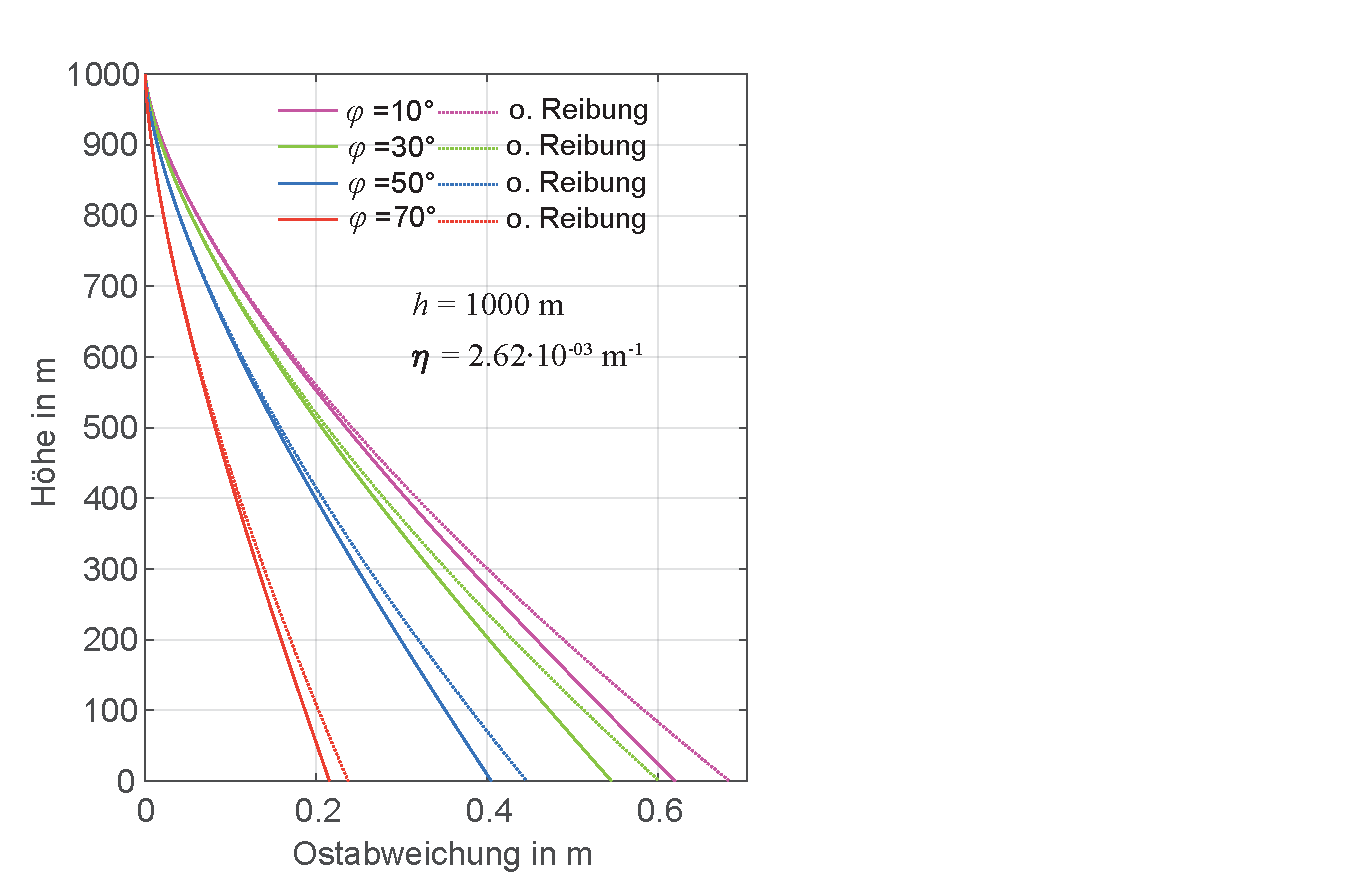
\includegraphics[width=0.8\columnwidth]{Lsg_Ballistik1.pdf}
\caption[Ostablenkung f�r den freien Fall einer Holzkugel]{Ostablenkung f�r den freien Fall einer Holzkugel von \SI{20}{\centi\metre} Durchmesser aus \SI{1000}{\meter} H�he mit und ohne Ber�cksichtigung der Luftreibung} \label{abb:bew_lsg_Ballistik1}
\end{figure}

\begin{figure}[H]
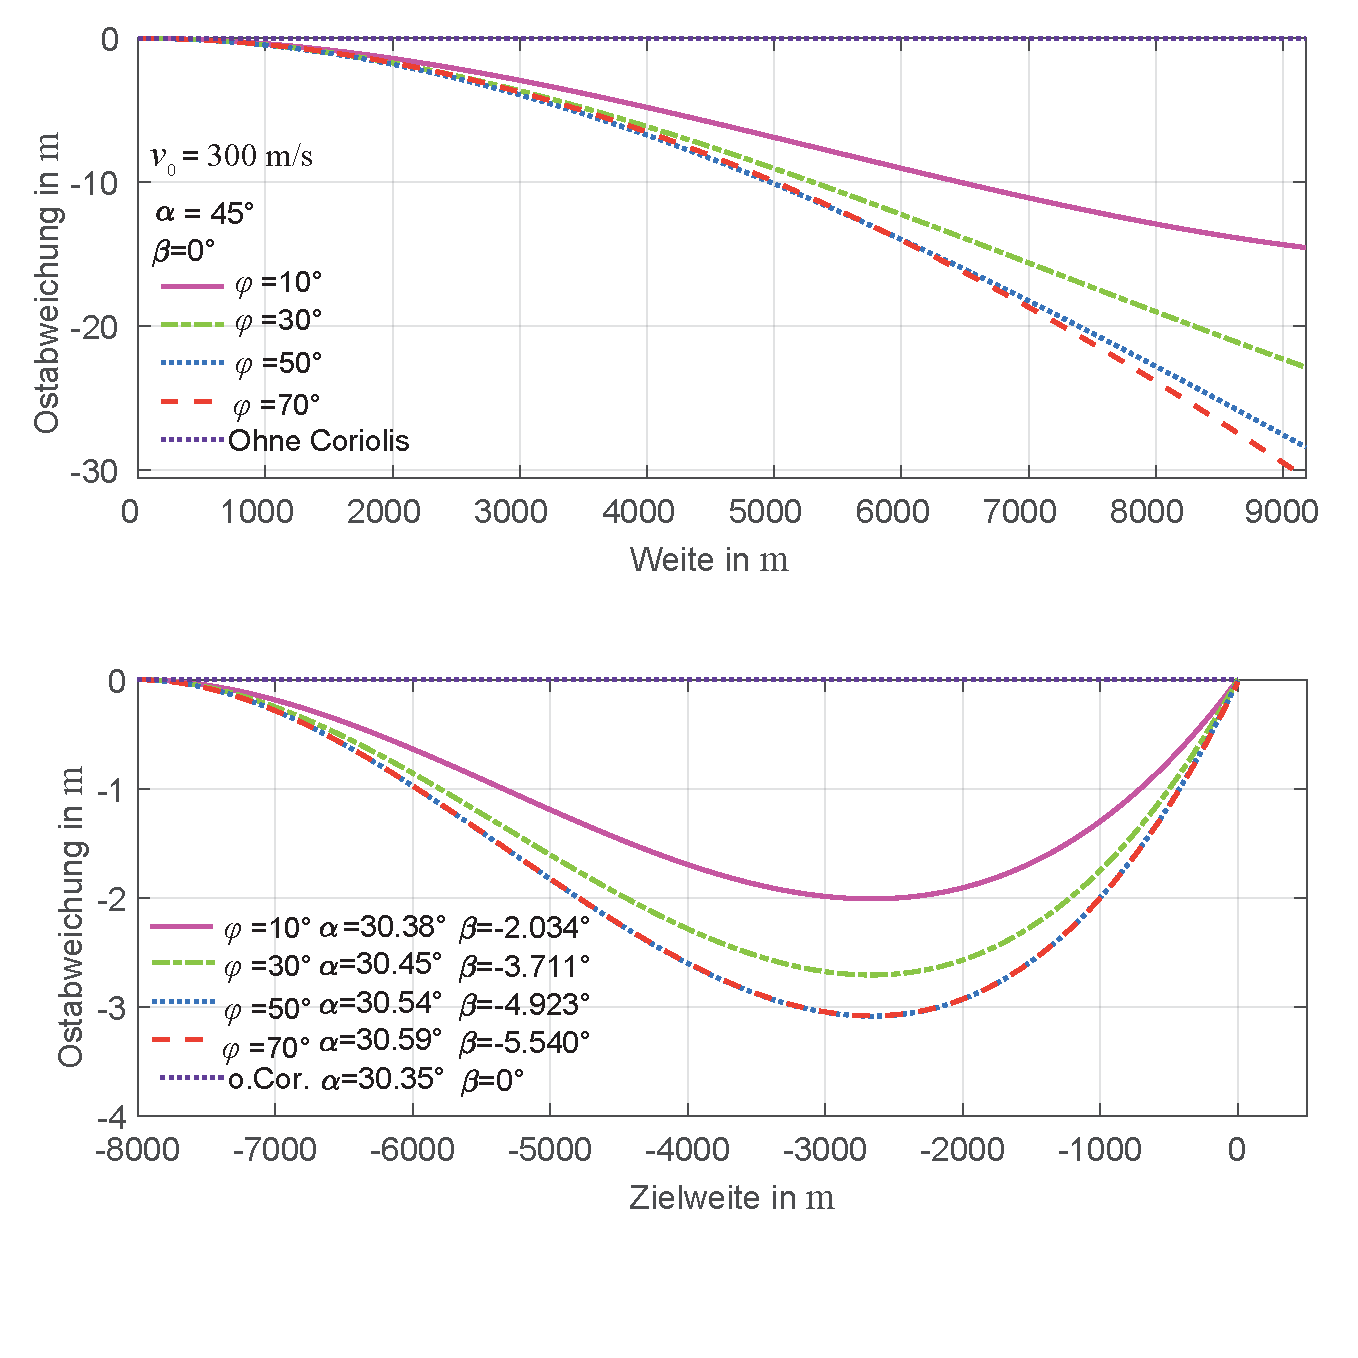
\includegraphics[width=0.75\columnwidth]{Lsg_BallistikCor_1.pdf}
\caption[Westablenkung eines nach S�den abgeschossenen Projektils]{Westablenkung eines mit $\SI{300}{\meter\per\second}$ nach S�den abgeschossenen Projektils f�r verschiedene geographische Breiten (oberes Bild) und Flugbahnprojektion auf die Horizontebene f�r einen Abschuss nach S�den mit eingestelltem Horizontal ($\alpha$)- und Vorhaltewinkel ($\beta$) um ein Ziel in 8000 m Entfernung zu treffen. Man beachte, dass negative Ostabweichung eine Westabweichung bedeutet} \label{abb:bew_lsg_BallistikCor_1}
\end{figure}

\begin{figure}[H]
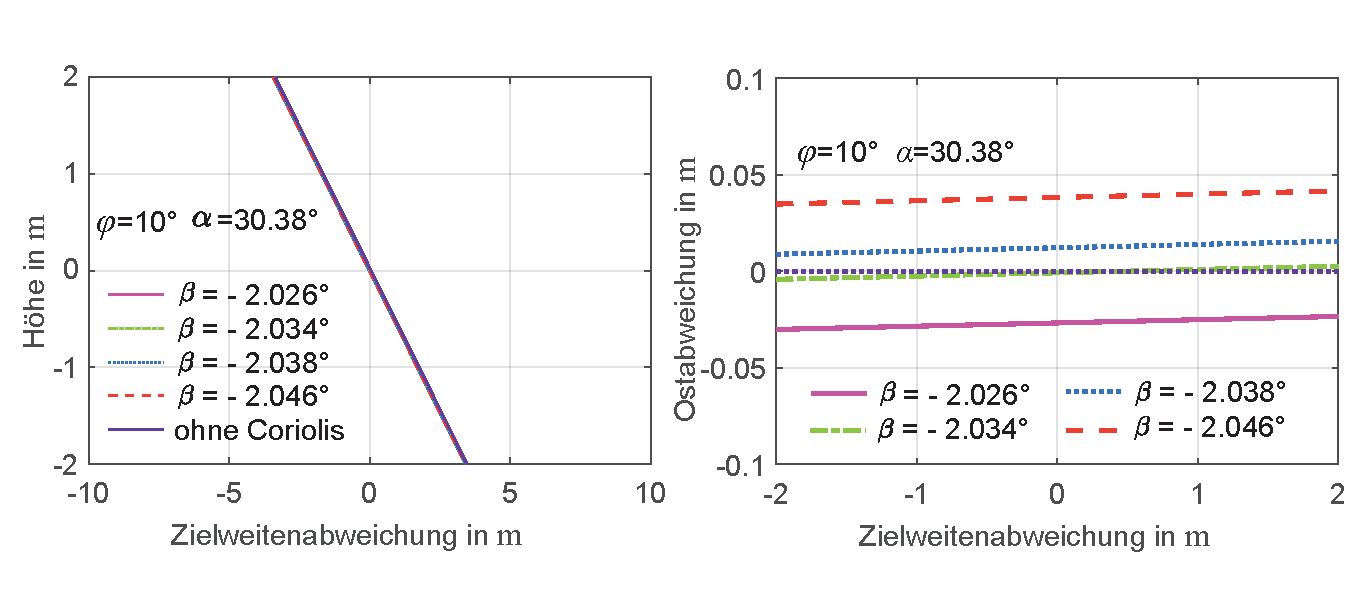
\includegraphics[width=\columnwidth]{Lsg_BallistikCor_2.pdf}
\caption[Verschiedene Vorhaltewinkel eines abgeschossenen Projektils]{Verschiedene Vorhaltewinkel eines mit $300 \:\mathrm{m/s}$ Richtung S�den abgeschossenen Projektils f�r eine geographische Breite von $\varphi = 10\degree$, um ein Objekt in 8000 m Entfernung zu treffen}\label{abb:bew_lsg_BallistikCor_2}
\end{figure}

\subprob{Exakte L�sung Ballistik} 

Die Bewegungsgleichungen lauten nun:
	\begin{align}
		\ddot{x}(t) &= + 2\omega \sin\!\varphi \:\dot{y} - \eta \,\dot{x} \,\lk \sqrt{\dot{x}^2+\dot{y}^2+\dot{z}^2} \rk^n \nonumber \\
		\ddot{y}(t) &= - 2\omega \sin\!\varphi \:\dot{x} - 2\omega \cos\!\varphi \:\dot{z} - \eta \,\dot{y} \,\lk \sqrt{\dot{x}^2+\dot{y}^2+\dot{z}^2} \rk^n \nonumber \\
		\ddot{z}(t) &= + 2\omega \cos\!\varphi \:\dot{y} - g - \eta \,\dot{z} \,\lk \sqrt{\dot{x}^2+\dot{y}^2+\dot{z}^2} \rk^n\,. \label{eq:lsg_BallistikCor2_1}
	\end{align}

Hierbei haben wir die Reibung mit dem Ansatz $- \eta \dot{x}_i^n$ ber�cksichtigt, aber offen gelassen, ob es sich um Stokes-Reibung ($ n=0 $) oder Newton-Reibung ($n=1$) handelt. 
F�r die Stokes-Reibung l�sst sich \eqref{eq:lsg_BallistikCor2_1} sogar exakt l�sen \cite{Neuberger1981}. 
Da in der Ballistik aber eher der Fall der Newton-Reibung relevant ist, werden wir diesen in Aufgabenteil 3 numerisch behandeln.
Zur L�sung f�r den reibungsfreien Fall $\eta=0$ leiten wir die Gleichung f�r $\ddot{y}$ aus \eqref{eq:lsg_BallistikCor2_1} noch mal nach der Zeit ab und erhalten:
\begin{align}
	\frac{\D^3}{\D t^3}{y}  &= - 4\omega^2 \,( \dot{y} \sin^2\!\varphi + \dot{y} \cos^2\!\varphi - 2\omega \,g \cos\!\varphi ) = - 4\omega^2 \,\dot{y} + 2\omega \,g \cos\!\varphi \nonumber \\
	\rightarrow \ddot{\zeta} + 4\omega^2 \,\zeta &= 2\omega \,g \cos\!\varphi \quad \text{mit} \quad \zeta = \dot{y} \,.\label{eq:lsg_BallistikCor2_2}
\end{align}
Die L�sung von \eqref{eq:lsg_BallistikCor2_2} ist gegeben durch
\begin{align}
	\zeta(t) = A\sin(2\omega\,t) + B\cos(2\omega\,t) + \frac{g \cos\!\varphi}{2\omega} \,. \label{eq:lsg_BallistikCor2_3}
\end{align}
Mit den Anfangsbedingungen $\zeta(0)=\dot{y}(0)=v_{0y}$ \bzw $\dot{\zeta}(0)=\ddot{y}(0) = -2\omega(\dot{x}(0) \sin\varphi + \dot{z}(0) \cos\varphi)$ bestimmen sich die Integrationskonstanten zu:
\begin{align}
	A &= -\lk\dot{x}(0) \sin\varphi + \dot{z}(0) \cos\varphi\rk = - (v_{0x} \sin\varphi + v_{0z} \cos\varphi) \nonumber \\
	B &=  v_{0y} - \frac{g \cos\varphi}{2\omega}\,. \label{eq:lsg_BallistikCor2_4}
\end{align}
Wir k�nnen \eqref{eq:lsg_BallistikCor2_3} noch mal integrieren und erhalten die L�sung f�r die Ost-West-Koordinate $y$ und analog f�r die anderen Koordinaten zu:
\begin{align}
	y(t) &= v_{0y}\,t + \frac{1}{2\omega} \lek A\, \lk 1- \cos(2\omega\,t) \rk - B\,\lk 2 \omega t-\sin(2\omega\,t) \rk \rek ~\,, \\
	x(t) &= v_{0x}\,t + \lek  A\, \lk t- \frac{\sin(2\omega\,t)}{2\omega} \rk + \frac{B}{2\omega} \lk 1 - \cos(2\omega\,t) \rk \rek \sin\varphi \nonumber \\ 
	& \ + g\,\cos\varphi\,\sin\varphi\,\frac{t^2}{2} ~\,, \\
	z(t) &= v_{0z}\,t - \frac{g}{2}\, t^2 + \lek  A\, \lk t- \frac{\sin(2\omega\,t)}{2\omega} \rk + \frac{B}{2\omega} \lek 1 - \cos(2\omega\,t) \rek \rek \cos\varphi \nonumber \\
	& \ + g\,\cos^2\varphi\,\frac{t^2}{2} \,.
 \label{eq:lsg_BallistikCor2_6}
\end{align}

F�r verschiedene geographische Breiten sind f�r einen Schuss in \figref{bew_lsg_BallistikCor_1} nach S�den unter $45\degree$ die erwarteten Abweichungen nach Westen aufgetragen.
Man erkennt, dass ein Ballistiker sehr wohl die Coriolis-Kraft ber�cksichtigen muss.
Die Effekte auf die H�he $z$ und die Schussweite $x_\text{max}$ sind dagegen Effekte der Gr��enordnung $(\omega \,t)^2$ und damit auf der Erde vernachl�ssigbar.
Wir stellen uns nun die Frage wie man die Schussrichtung w�hlen muss, damit man die Corioliseffekte ausgleicht.
Dazu muss man offensichtlich die Schussrichtung um einen Winkel $\beta$ nach Osten �ndern, um die Westablenkung zu kompensieren.
Die Schussweite ist n�herungsweise gegeben durch 
\begin{align}
	x_\text{max} \approx \frac{{v_0}^2\sin(2\alpha)\,\cos(\beta)}{g} = \SI{8000}{m} \,, \label{eq:lsg_BallistikCor2_7}
\end{align}
und die Westablenkung durch $y(t_\text{max})$ , worin $t_\text{max} \approx 2v_{0z}/g = 2 v_0 \sin\alpha$ die Flugzeit bis zum Auftreffpunkt ist.
Aus diesen beiden Gleichung lassen sich der  Winkel $\alpha$ gegen die Horizontale und der Richtungswinkel $\beta$ gegen die S�drichtung bestimmen.
In einer erster N�herung kann man dabei den Effekt der Winkel�nderung $\beta$ auf die Weite separieren.
Man bestimmt also zun�chst $\alpha$ aus \eqref{eq:lsg_BallistikCor2_7} mit dem Startwert $\beta = 0$, daraus dann aus \eqref{eq:lsg_BallistikCor2_6} mit $y(8000 \mathrm{m})=0$ numerisch den verbesserten Winkel $\beta'$ und wiederholt das bis eine hinreichende Genauigkeit erreicht ist.
Das Ergebnis ist in \figref{bew_lsg_BallistikCor_2} dargestellt, die Rechnungen sind in \mlbewref{BallistikCoriolis02.m} ausgef�hrt.

\begin{figure}[H]
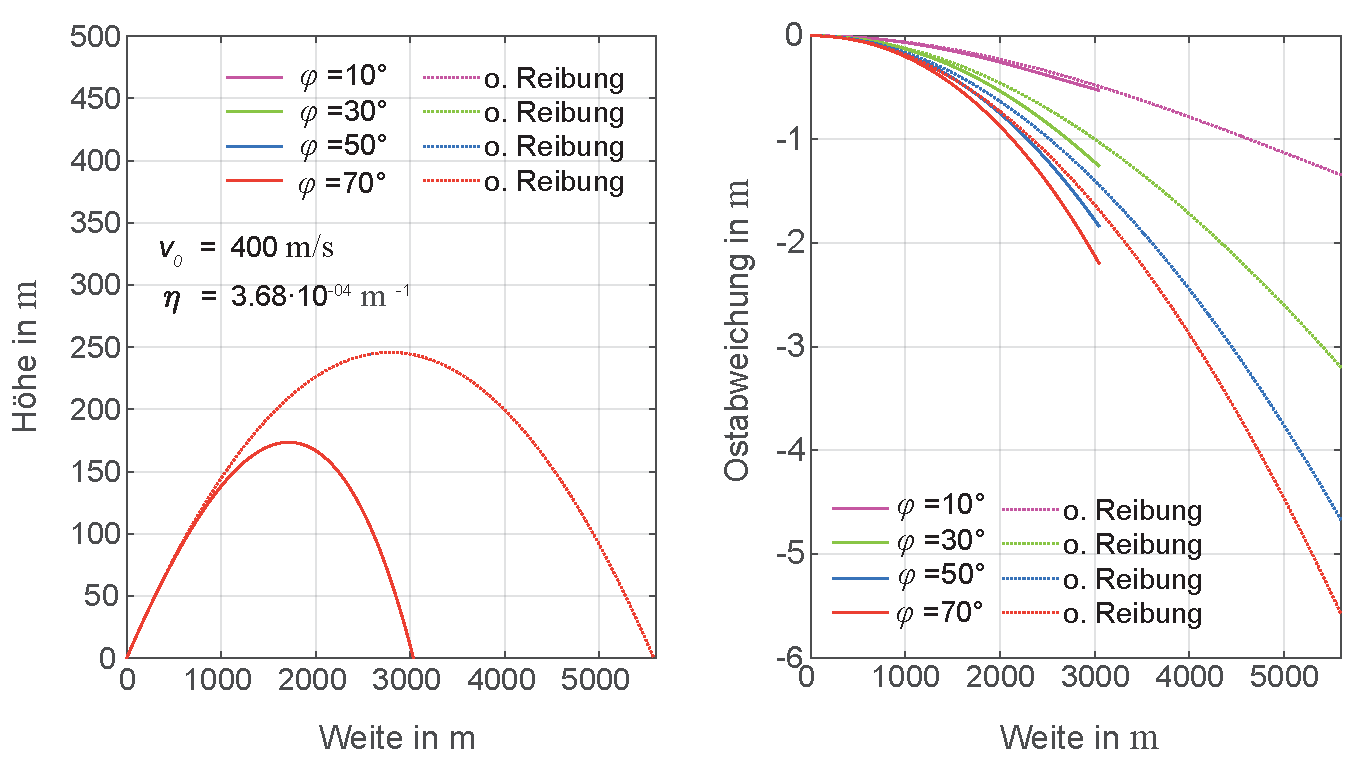
\includegraphics[width=\columnwidth]{Lsg_BallistikCor_3.pdf}
\caption[Flugbahn und Westablenkung einer abgeschossenen Kanonenkugel]{Flugbahn und Westablenkung einer mit $400 \mathrm{m/s}$ nach S�den abgeschossenen Kanonenkugel mit und ohne Ber�cksichtigung von Luftreibung bei verschiedenen geographischen Breiten (Horizontalwinkel $\alpha = 10\degree$)} \label{abb:bew_lsg_BallistikCor_3}
\end{figure}

\subprob{Numerische L�sung bei Reibung}
Wir wollen nun das DGL-System \eqref{eq:lsg_BallistikCor2_1} numerisch mit \matlab{} l�sen und zwar f�r den Fall der Luftreibung, die man gut mit der Newton-Reibung beschreiben kann:
\begin{align*}
	\eta = \frac{3}{4} \,c_\text{w} \,\frac{\varrho_\text{L}}{\varrho_\text{K}}\,\frac{1}{D_\text{K}} \,,
\end{align*}
worin $D_\text{K}$ der Durchmesser der Kanonenkugel ist.
Um das DGL-System numerisch mit der \matlab-Routine \odevf{} l�sen zu k�nnen, schreiben wir dieses um, in dem wir den Vektor $Y=(Y_1,Y_2,\ldots,Y_6)^\text{T}$ einf�hren, mit $Y_1 = x, Y_2 =\dot{x}, Y_3 = y, Y_4 = \dot{y}, Y_5 = z, Y_6 = \dot{z}$ Dann kann \eqref{eq:lsg_BallistikCor2_1} mit $v=\sqrt{\dot{x}^2+\dot{y}^2+\dot{z}^2} $ schreiben als:
\begin{align}
	\frac{\D}{\D t} \lk
	\begin{array} {c}
		 Y_1\\Y_2\\Y_3\\Y_4\\Y_5\\Y_6 
	\end{array} \rk
	= \lk \begin{array} {c}
		 \dot{x}\\ \ddot{x}\\ \dot{y}\\ \ddot{y}\\ \dot{z}\\ \ddot{z}
	\end{array} \rk
	= \lk \begin{array} {l}
		Y_2\\  2\omega\,\sin\!\varphi \:Y_4 - \eta\,v\:Y_2  \\ Y_4 \\ - 2\omega\,\sin\!\varphi \:Y_2 - 2\omega\,\cos\!\varphi \:Y_6 - \eta\,v\:Y_4 \\ Y_6 \\ 2\omega\,\sin\!\varphi \:Y_4 - g - \eta\,v\:Y_2 	\end{array} \rk \,.
\label{eq:lsg_BallistikCor3_1}
\end{align}

\newpage
Die Anfangsbedingungen sind f�r den freien Fall (Aufgabenteil 1) \bzw die Ballistik (Aufgabenteil 2) gegeben durch:
\begin{align*}
	Y_0 = \lk 	\begin{array} {c} 0 \\ 0 \\ 0 \\ 0 \\ h \\ 0	\end{array} \rk ~~~\text{\bzw}~~~~ Y_0 = \lk 	\begin{array} {c}  0 \\ v_\text{x0} \\ 0 \\ v_\text{y0} \\ 0 \\ v_\text{z0}  
	\end{array} \rk \,.
\end{align*}
%Der Funktionsaufruf f�r das DGL-System f�r die Routine \odevf{} lautet:\\
%\begin{lstlisting} [frame=single]
%% Differentialgleichungssystem f�r Coriolis-Kraft
%function dY = CoriolisDGLS(t,Y,Omeg,Cphi,Sphi,G,Eta)
  %dY    = zeros(6,1);
  %dY(1) = Y(4); dY(2) = Y(5); dY(3) = Y(6);
  %vbet  = sqrt(Y(4)^2+Y(5)^2+Y(6)^2);
  %dY(4) = 2*Omeg*Sphi*Y(5)-Eta*vbet*Y(4);
  %dY(5) = -2*Omeg*Sphi*Y(4)-2*Omeg*Cphi*Y(6)-Eta*vbet*Y(5);
  %dY(6) = 2*Omeg*Cphi*Y(5)-G-Eta*vbet*Y(6);  
%end
%\end{lstlisting} 
%\medskip
Das Ergebnis der Rechnungen ist in \figref{bew_lsg_BallistikCor_3} dargestellt und in \mlbewref{BallistikCoriolis03.m} im Detail hinterlegt.
Man erkennt, dass die Luftreibung sowohl die Schussweite als auch die Westablenkung reduziert.
Ein Ballistiker muss also beide Effekte und die geographische Breite ber�cksichtigen.



\end{subprobs}
\end{sol} 
%\href{PhysikUncut_Part1.pdf#prb:bew_Coriolis_I}{\textcolor{blue} {$\rightarrow$ zur \probref{bew_Coriolis_I}.}}\\
\textcolor{blue} {$\rightarrow$ zur} \probref{bew_Coriolis_I}.\\
\noindent\rule[1ex]{\textwidth}{0.5pt}  \newpage  


%-----------------------------------------------------------------------------------------------------------
\hypertarget{lsg:bew_Coriolis_II}{}
\begin{sol}{prob:bew_Coriolis_II}\label{lsg:bew_Coriolis_II}%�bung19
\textbf{Coriolis-Kraft II -- Fluss- und Schienenabtrag}

\begin{subprobs}
	\subprob{Flussabtrag}
	Ein gro�er Fluss str�mt im Mittel%
        \footnote{Wir nehmen hier nicht ganz richtig an,
        dass die Flie�geschwindigkeit �berall im Fluss
        gleich gro� ist.
        Wir werden sp�ter in \autoref{chap:kontmech} sehen,
        dass dies nicht der Fall ist.}
        mit $\dot{x}' = v' = - \SI{2}{\meter\per\second}$ nach Norden
        ($\varphi = 50\degree$ geographische Breite)
        und ist maximal $B = 2$ km breit.
        Die Coriolis-Beschleunigung in $y'$-(Ost)-Richtung ist dann $a_\text{Cor} = - 2 v' \omega \sin \varphi \approx 2.2 \, 10^{-4} \,\SI{}{\meter\per\second\squared} \approx 2.3\, 10^{-5}\: g$, also relativ klein.
        Coriolis- und Schwerebeschleunigung ergeben damit eine resultierende Beschleunigung, die normal zur Wasseroberfl�che sein muss. 
	Demzufolge steht die Wasseroberfl�che unter einem Winkel $\alpha$.
        Mit $\tan \alpha = H/B = a_\text{Cor}/g$ ergibt sich dann
		\[ H = \frac{- 2 B v' \omega \,\sin\varphi}{g} \approx \SI{4.5}{cm}\,.
	\]
Das Wasser eines 2 km breiten nach Norden flie�enden Stroms in Sibirien ($\varphi \approx 50 \degree $) kann also tats�chlich am �stlichen Ufer etwas h�her stehen als am westlichen.
Theoretisch w�re es also denkbar, dass sich der Fluss nach rechts mit der Zeit an das Ufer heranarbeitet.
Vorherrschende Winde aus West haben aber mindestens den gleichen Einfluss. 
\subprob{Schienenbeeinflussung}
Bei einem ICE ist $v_\text{max}' = 330$ km/h, die Schienenbreite der Normalspur betr�gt 1435~mm. Daraus ergibt sich in den gem��igten Breiten eine H�he $H$ von \ca 1.5~mm, was um etwa eine Gr��enordnung geringer ist als die Toleranzen bei der Gleisverlegung.
Jede noch so gro�e Kurve h�tte einen st�rkeren Effekt auf die unterschiedliche Abnutzung der beiden Schienen.
Es ist immer wieder erstaunlich, wie hartn�ckig sich die Mythen der Auswirkung der Coriolis-Kraft in solchen Effekten (auch Drehrichtung des abflie�enden Wassers im Waschbecken) �ber Generationen von Physikb�chern halten.
Vielleicht steckt dahinter der Wunsch, dass die Effekte der Physik doch offensichtlicher auftreten sollen.
Wir finden aber, dass gerade die Subtilit�t der physikalischen Effekte diese so interessant machen, ansonsten w�ren sie ja \anf{nichts Besonderes}.
\end{subprobs}

\end{sol} 
%\href{PhysikUncut_Part1.pdf#prb:bew_Coriolis_II}{\textcolor{blue} {$\rightarrow$ zur \probref{bew_Coriolis_II}.}}\\
\textcolor{blue} {$\rightarrow$ zur} \probref{bew_Coriolis_II}.\\
\noindent\rule[1ex]{\textwidth}{0.5pt}  \newpage  

%-----------------------------------------------------------------------------------------------------------
\hypertarget{lsg:bew_Coriolis_III}{}
\begin{sol}{prob:bew_Coriolis_III}\label{lsg:bew_Coriolis_III}%�bung20
\textbf{Coriolis-Kraft III -- Wetterph�nomene} \\ \\
Die Effekte der Coriolis-Kraft \eqref{eq:bew_Coriolis_Kraft}  wirken auch auf sich bewegende Luftmassen.
Die Bewegung von Luftmassen ist als Druckausgleich vom Hochdruck- zum Tiefdruck-Gebiet zu verstehen.
Tiefdruckgebiete entstehen beispielsweise dadurch, dass sich die Luft am Boden stark erhitzt und nach oben steigt.
\begin{subprobs}
	\subprob{Passatwinde}
	Luftmassen str�men zum relativ stabilen Tiefdruckgebiet entlang des �quators hin, d.h. es entsteht eine N-S-Bewegung auf der Nordhalbkugel \bzw eine S-N-Bewegung auf der S�dhalbkugel, wie in \figref{bew_ZyklonPassat}\,a dargestellt.
	In \eqref{eq:bew_BGL_Erdrotation_Ko} ist dann $\dot{x}' > 0$ und n�herungsweise $\dot{y}' = \dot{z}' = 0$, so dass es zu einer Kraft in West-Richtung $\propto - 2\omega \,\dot{x}' \,\sin{\varphi}$ kommt.
        Auf der S�dhalbkugel ist $\sin{\varphi} <0$, aber auch $\dot{x}' < 0$, so dass es wiederum zu einer West-Ablenkung kommt.
        Der resultierende Effekt sind die relativ stabilen Passatwinde.
	
\begin{figure}
\centering
\includegraphics[width=\textwidth]{ZyklonPassat.pdf}
\caption[Entstehung von Passatwinden und eines au�ertropischen Zyklons]{\fa Entstehung von Passatwinden \fb Entstehung eines au�ertropischen Zyklons auf der Nord- \bzw S�dhalbkugel (oberes \bzw unteres Bild)}\label{abb:bew_ZyklonPassat}
\end{figure}

\subprob{Zyklonen auf der Nord- und S�dhalbkugel}
	\begin{itemize}[a) ]
		\item Luftstr�mung vom Hoch zum Tief, Nordhalbkugel\\
	In der \figref{bew_LsgCoriolisIIIa} ist die Luftmassenbewegung vom Hoch- zum Tiefdruckgebiet auf der Nordhalbkugel dargestellt.
        Wenn sich die Luftmasse nach Norden bewegt, findet wegen der Coriolis-Kraft eine Ablenkung nach Osten, also aus Sicht der bewegten Luftmasse nach rechts statt.
        Entsprechend wird ein Wind, der von Westen auf das Tiefdruckgebiet zustr�mt, s�dlich abgelenkt.
        Aus Sicht der bewegten Luftmasse ist das wieder eine Rechtsablenkung.
        Da Winde immer von Hoch- zu Tiefdruckgebieten wehen, f�hrt diese Rechtsablenkung auf der Nordhalbkugel zu einer Drehung gegen den Uhrzeigersinn um das Zentrum des Tiefdruckgebiets.
        Zus�tzliche wird diese Drehung bei thermischen Tiefs im Zentrum noch durch den Aufstieg der warmen Luft nach oben �berlagert.
        Die resultierende Luftmassenbewegung kann eine entsprechende Spirale bilden.
        Damit haben wir das Entstehen von (au�ertropischen) Zyklonen auf der Nordhalbkugel beschrieben (Abb. oberes Bild in \figref{bew_ZyklonPassat}\,b).
        Die gleichen Effekte treten bei Hurrikans auf, bei denen das Tiefdruckzentrum bei ausreichender hoher Temperatur durch Verdunstung �ber der Meeresoberfl�che entsteht.

\begin{figure}[H]\centering
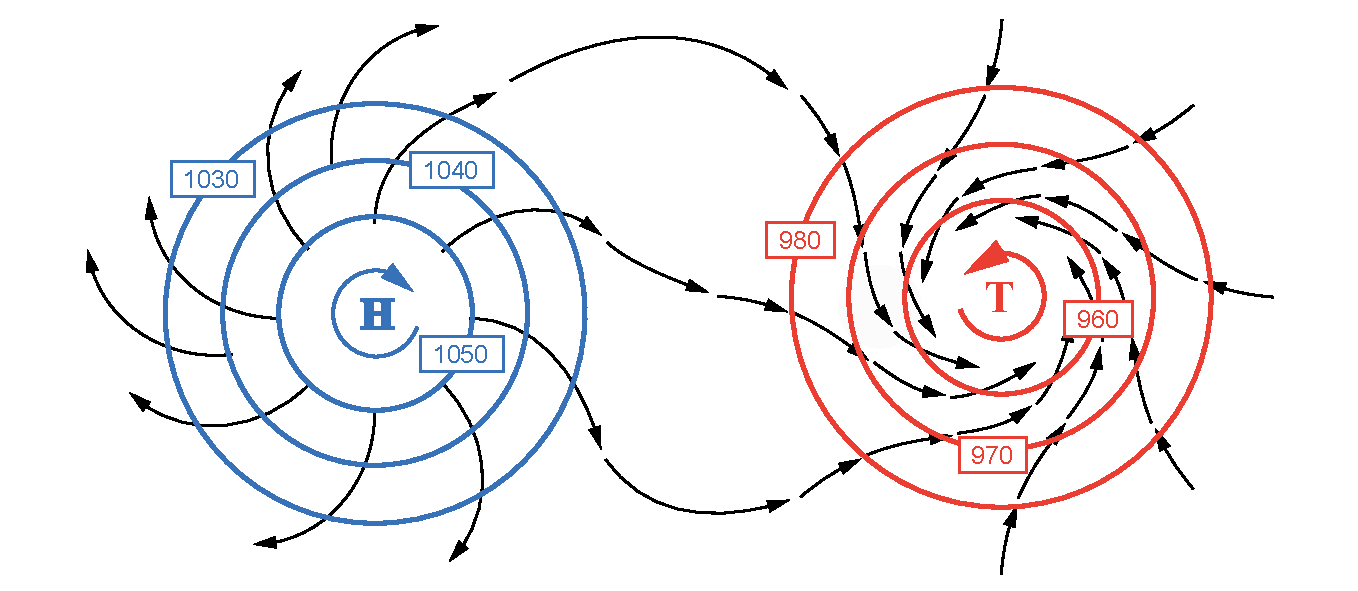
\includegraphics[width=\textwidth]{DruckausgleichHT01.pdf}
\caption[Druckausgleich zwischen Hoch- und Tiefdruckgebieten]{Druckausgleich zwischen Hoch- und Tiefdruckgebieten, die unser Wetter wesentlich beeinflussen. Dargestellt ist die Situation auf der Nordhalbkugel, wo die Luftmassen vom Hoch- zum Tiefdruckgebiet str�men und dabei nach rechts abgelenkt werden. Auf der S�dhalbkugel werden Sie entsprechend nach links abgelenkt (nicht dargestellt). Man beachte, dass diese Darstellung den Ausgleich am Boden zeigt}\label{abb:bew_LsgCoriolisIIIa}
\end{figure}

	\item Luftstr�mung vom Hoch zum Tief, S�dhalbkugel\\
	Auf der S�dhalbkugel wird die Luftmasse, die sich nach S�den bewegt �stlich abgelenkt, was gemessen in Windrichtung dann einer Linksablenkung entspricht.
        Auf der S�dhalbkugel f�hrt diese Linksablenkung dann zu einer Drehung im Uhrzeigersinn. (Abb. unteres Bild in \figref{bew_ZyklonPassat}\,b).

\begin{figure}[H]\centering
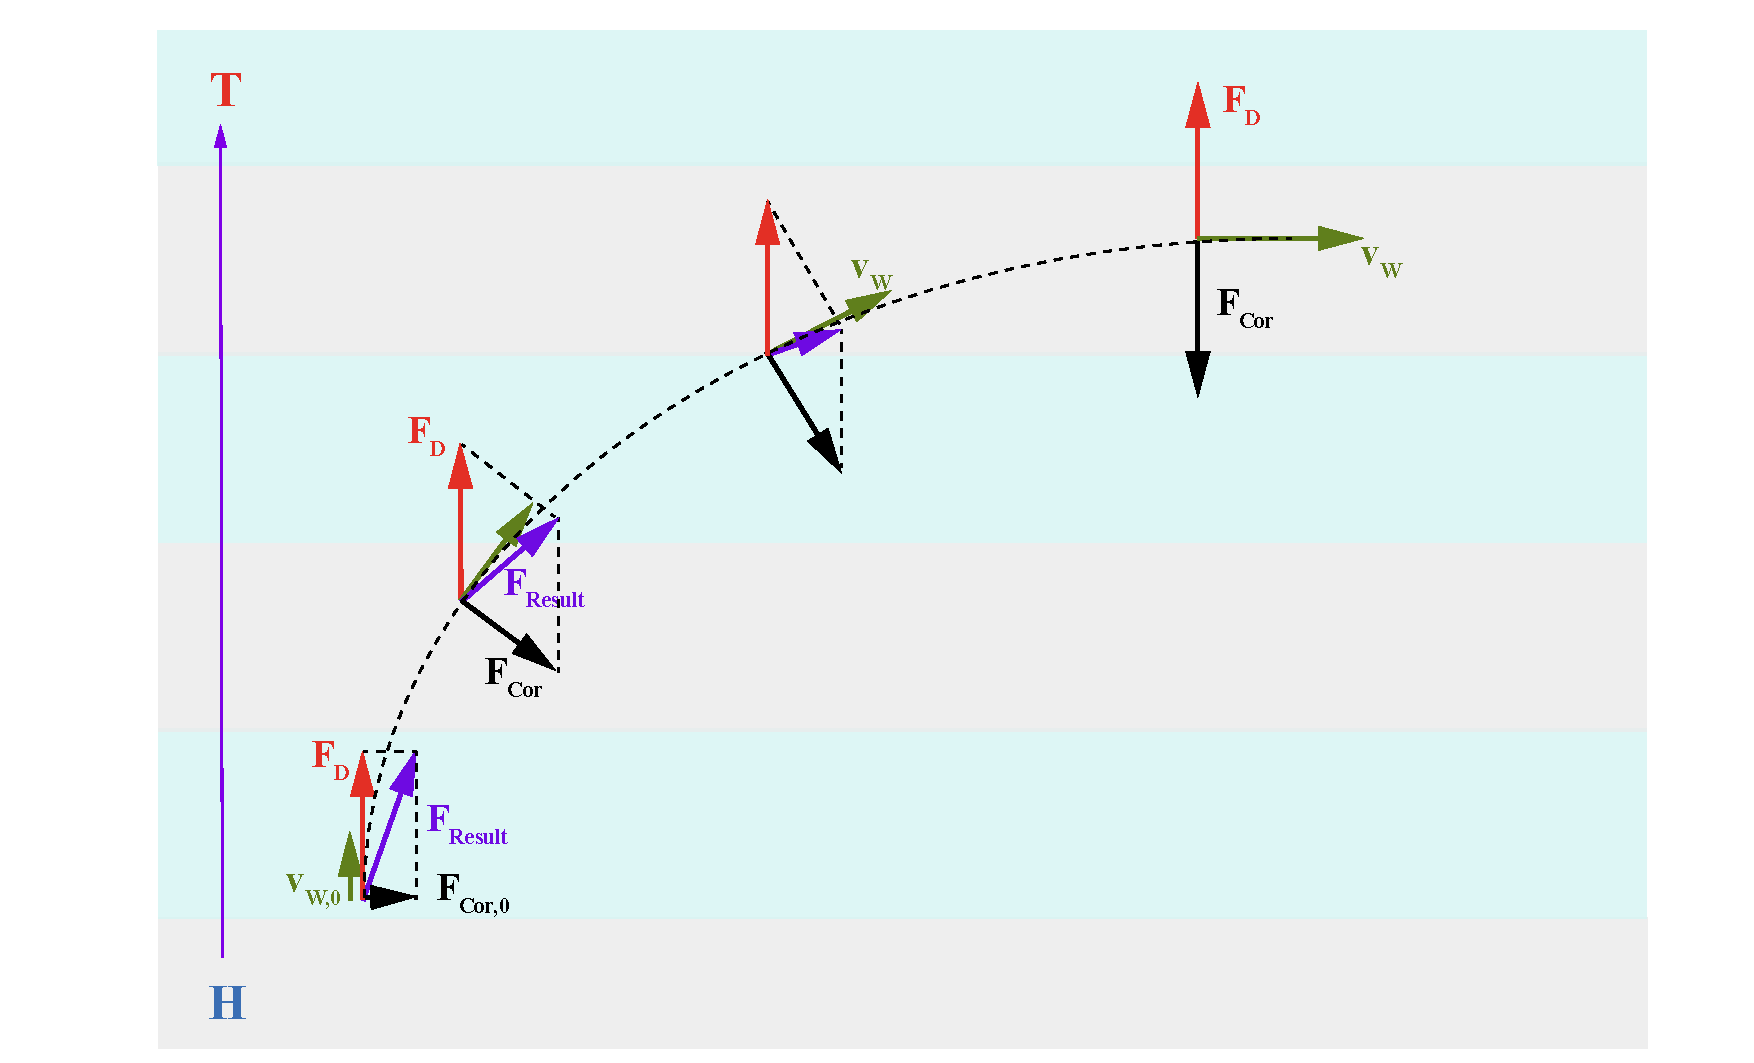
\includegraphics[width=\textwidth]{DruckausgleichHT02.pdf}
\caption[Einstellung der Windrichtung und Windgeschwindigkeit]{Einstellung der Windrichtung und Windgeschwindigkeit durch Zusammenwirkung von Druckgradientenkraft und Coriolis-Kraft auf der Nordhalbkugel nach \cite{Brauner2019}. Bei dieser Darstellung haben wir die Reibung, die unweigerlich am Boden auftritt, vernachl�ssigt. Man kann sich leicht �berlegen, dass diese dazu f�hrt, dass der station�re Geschwindigkeitsvektor nicht genau senkrecht auf dem Druckgradienten steht. die hier gezeigte Darstellung entspr�che also in etwa den Verh�ltnissen in einer H�henstr�mung }\label{abb:bew_LsgCoriolisIIIb}
\end{figure}

	\end{itemize}

\subprob{Windrichtung/-st�rke in Nordschottland und in Deutschland}
Um die Windrichtung und Windgeschwindigkeit zu berechnen, betrachten wir \figref{bew_LsgCoriolisIIIb}. 
Senkrecht zu den Isobaren wirkt durch den Druckgradienten die so genannte Druckgradientenkraft $\vec{F}_\text{D}$, die die Luftmassen in Bewegung setzt.
Diese werden durch die Coriolis-Kraft $\vec{F}_\text{Cor}$ nach rechts abgelenkt.
Station�res Gleichgewicht und damit die stabile Ausbildung einer Windrichtung ist dann gegeben, wenn die Coriolis-Kraft genau entgegengesetzt gleich der Druckgradientenkraft ist.
Dann str�mt der Wind in etwa parallel zu den Isobaren.
Wir k�nnen die Windgeschwindigkeit durch folgende �berlegungen absch�tzen.
Der Luftdruckunterschied $\Delta p$ �ber eine Distanz $\Delta s$ erzeugt auf ein Querschnittsfl�che $A$ und damit auf ein kleines Luftvolumen $A \Delta s$ eine Druckgradientenkraft mit einem Betrag von:
\begin{align*}
	F_\text{D} = \lk \frac{\Delta p} {\Delta s}\rk  A  \Delta s~.
\end{align*}
Wir betrachten nun ein Luftvolumen der Masse $\Delta m = \varrho_\text{L} A \Delta s$, 
welches sich mit der Geschwindigkeit $v$ in der geographischen Breite $\varphi$ bewegt.
Der Betrag der Coriolis-Kraft, der auf dieses Luftvolumen wirkt, ist
\begin{align*}
	F_\text{Cor} = 2 \Delta m \,\omega \,v \,\sin\varphi= 2 \omega \,v \,\sin\varphi \,\varrho_\text{L}\,A\,\Delta s~.
\end{align*}
Gleichsetzen von $F_\text{D}$ und $F_\text{Cor}$ und umstellen nach $v$ ergibt:
\begin{align}
	v = \frac{1}{2 \varrho_\text{L} \,\omega \,\sin\varphi} \frac{\Delta p}{\Delta s}\,. \label{eq:bew_Windgeschwindigkeit}
\end{align}
Der H�henwind (auch geostrophischer Wind genannt) ist also von der Dichte der Luft $\varrho_\text{L}$, der geographischen Breite $\varphi$ und dem Isobarenabstand $\Delta p / \Delta s$ abh�ngig.\footnote{Dieser so berechnete Wind kann in Bodenn�he durch Reibungseffekte auf etwa 2/3 sinken und auch in seiner Richtung ver�ndert werden.}

Im gegebenen Beispiel weht der Wind �ber Nordschottland vom Hochdruckgebiet �ber den Azoren kr�ftig in Richtung Osten bis Nordosten.
Die Windrichtung ist definiert als Herkunftsrichtung eines Windes, also sprechen wir hier von einem Westwind \bzw S�dwestwind. 
In Mitteleuropa ist der Wind wegen der geringen Luftdruckunterschiede sehr schwach.
Allgemein gilt: je gr��er der Abstand der Isobaren, desto geringer die Windgeschwindigkeit.
Und im Umkehrschluss: je geringer der Abstand der Isobaren, desto gr��er die Windgeschwindigkeit. 
\end{subprobs}

\end{sol} 
%\href{PhysikUncut_Part1.pdf#prb:bew_Coriolis_III}{\textcolor{blue} {$\rightarrow$ zur \probref{bew_Coriolis_III}.}}\\
\textcolor{blue} {$\rightarrow$ zur} \probref{bew_Coriolis_III}.\\
\noindent\rule[1ex]{\textwidth}{0.5pt}  \newpage 

%-----------------------------------------------------------------------------------------------------------
\hypertarget{lsg:bew_Coriolis_IV}{}
\begin{sol}{prob:bew_Coriolis_IV}\label{lsg:bew_Coriolis_IV}%�bung21
\textbf{Coriolis-Kraft IV -- Karussell} \\ \\
Die wirkenden Kr�fte auf einen bewegten K�rper sind in \figref{bew_Lsg_Scheibe01} dargestellt.

\begin{figure}[H]\centering
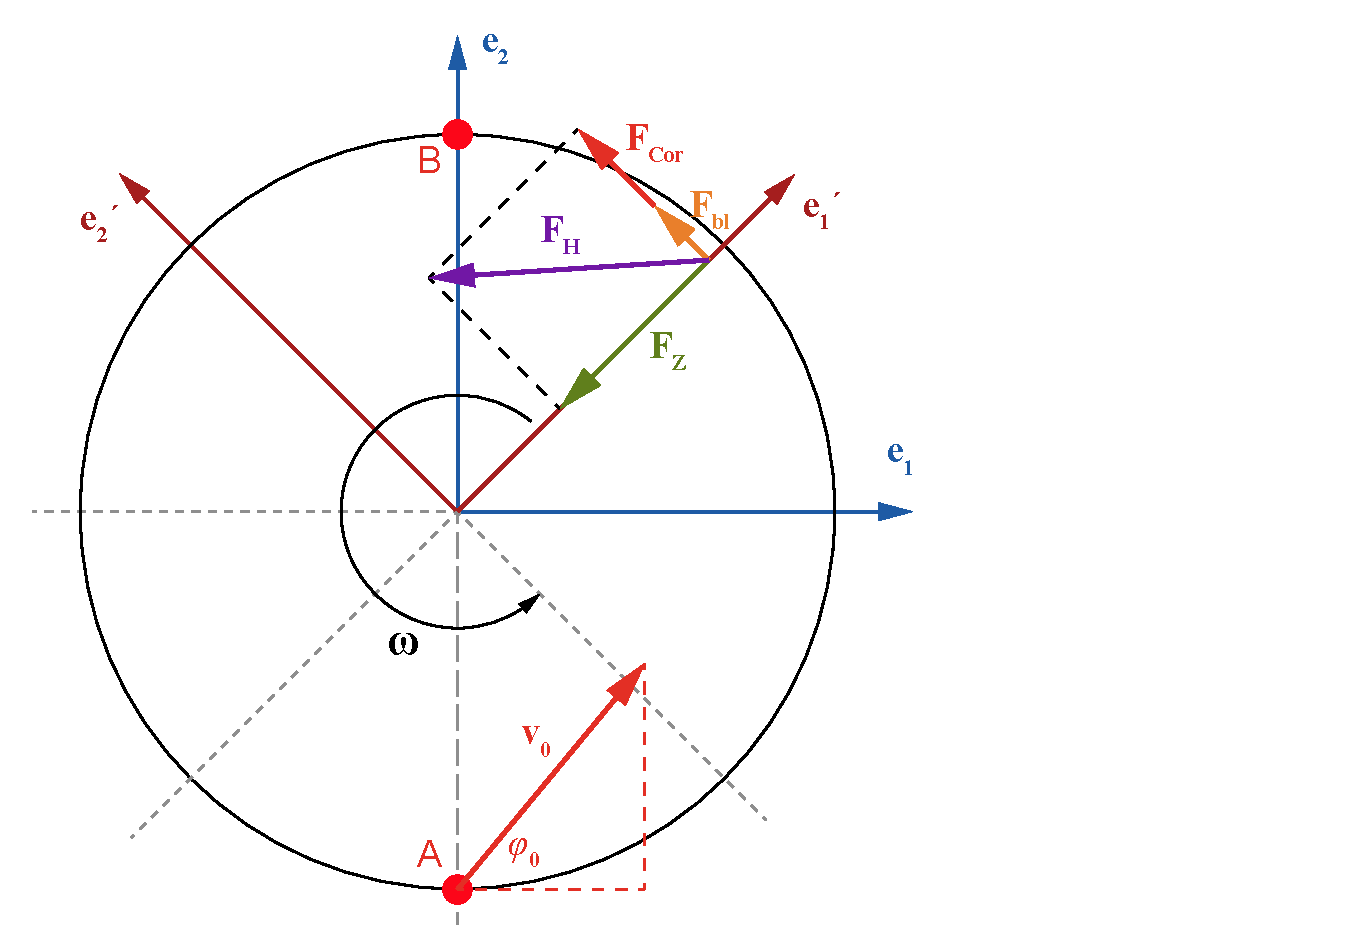
\includegraphics[width=0.8\textwidth]{Lsg_Scheibe01.pdf}%
\caption[Kr�fte auf einen bewegten K�rper auf einem sich drehenden Karussell]{Kr�fte auf einen bewegten K�rper auf einem sich drehenden Karussell. Angegeben sind die Tr�gheitskr�fte $\vec{F}_\text{Z}',\vec{F}_\text{Cor}',\vec{F}_\text{br} $, worin $\vec{F}_\text{br}$ die Euler-Kraft ist. Ebenso eingezeichnet ist die Haftreibungskraft $\vec{F}_\text{H}$ und die Richtung der Anfangsgeschwindigkeit $\vec{v}_0$ des K�rpers}
\label{abb:bew_Lsg_Scheibe01}
\end{figure}

\begin{subprobs}
\subprob{Haftreibung des Reifens}
Die Bewegungsgleichung in vektorieller Form lautet:
	\begin{align}
			m \,\ddot{\vec{r}}' &= \vec{F}_\text{R} -m\,\vec{\omega}'\times[\vec{\omega}'\times\vec{r}']-2m \,\vec{\omega}'\times\vec{v}'-m\,\dot{\vec{\omega}}\times\vec{r}' \,, \nonumber \\
		&=	\vec{F}_\text{R}+\vec{F}_\text{Z}'+\vec{F}_\text{Cor}' + \vec{F}_\text{br} \,, \label{eq:bew_lsg_Karussell_1}
	\end{align}
worin $\vec{F}_\text{R}$ die Reibungskraft ist, die durch die Reifen auf der Unterlage des Karussells aufzubringen ist.
Da sich das Go-Kart gleichf�rmig mit $v_0$ bewegen soll, muss die dazu notwendige Motor- \bzw Bremskraft ebenfalls �ber die Reibung auf den Boden des Karussells vermittelt werden.
Wir wollen nun die einzelnen Kraft-Komponenten bestimmen.
Aus der vektoriellen Zerlegung nach \figref{bew_Lsg_Scheibe01} ergibt sich ($\vec{\omega}$ zeigt aus der Bildebene heraus):
	\begin{align}
			m \,\ddot{\vec{r}}' &= 0 \,, \nonumber \\
			\Rightarrow \vec{F}_\text{R} &= m \,\vec{\omega}' \times\lk\vec{\omega}'\times\vec{r}'\rk+2m\,\lk\vec{\omega}'\times \dot{\vec{r}}'\rk+m\,\lk\dot{\vec{\omega}}'\times\vec{r}'\rk \,. \label{eq:bew_lsg_Karussell_2}
	\end{align}
Wir k�nnen die Kraft in die Komponenten der Achsen des mitbewegten KOS zerlegen und erhalten f�r:
	\begin{align*}
		\vec{F}_\text{R,1} &=  -m\,\omega'^2 \,r' \:\vecpeX \,,\\
		\vec{F}_\text{R,2} &= +2m\,\omega'\,v'\:\vecpeY + m\,\dot{\omega}'\,r'\:\vecpeY \,.
	\end{align*}
Die Coriolis-Kraft und die Euler-Kraft zeigen also in die gleiche Richtung.
Dennoch kann man die beiden in $\vec{\Sigma}'$ unterscheiden, da die erste nur auf einem bewegten K�rper wirkt. \\
Wir setzen f�r die Reibungskraft nun eine Kraftreibung mit $\vec{F}_\text{R} = \vec{F}_\text{H} = -\mu_\text{H} m g \dot{\vec{r}} /\left| \dot{\vec{r}}\right|$ an.
Dies ist f�r den Reifenkontaktpunkt eine gute N�herung.
Die gesamte Haftreibung, die aufgebracht werden muss ist (wir lassen der Einfachheit halber die Striche weg):
		\begin{align}
				|\vec{F}_\text{H}| &= m\sqrt{\omega^4 \,r^2+4 \omega^2\, v^2 +\dot{\omega}^2 \,r^2+4 \omega \,\dot{\omega}\, v \,r } \,, \nonumber \\
				|\vec{F}_\text{H}| &= m \,\omega\, r\sqrt{\omega^2+4\frac{v^2}{r^2}+\bigg(\frac{\dot{\omega}}{\omega}\bigg)^2+4\frac{\dot{\omega}v}{\omega r}} \,, \nonumber \\
				m \,\mu_\text{H} \,g &= m\, \omega\, r \sqrt{\omega^2+\bigg(2\frac{v}{r}+\frac{\dot{\omega}}{\omega}\bigg)^2} \,, \nonumber \\
				\mu_\text{H} &= \frac{\omega \,r}{g} \sqrt{\omega^2+\bigg(2\frac{v}{r}+\frac{\dot{\omega}}{\omega}\bigg)^2} \,.\label{eq:bew_lsg_Karussell_3} 
		\end{align}
Nun wollen wir die Frage beantworten, ab welcher Geschwindigkeit $v$ oder Position $r$ das Go-Kart ins Rutschen kommt.
F�r $v_\text{max}$ ergibt sich:
	\begin{align*}
				v_\text{max} = \frac{r \,\omega}{2}\,\lk \sqrt{\bigg(\frac{\mu\, g}{r}\bigg)^2-1}-\frac{\dot{\omega}}{\omega^2}\rk \,.
	\end{align*}
F�r $r_\text{max}$ bei Annahme $\dot{\omega}=0$:
	\begin{align*}
			r_\text{max} =\frac{1}{\omega^2}\sqrt{(\mu\, g)^2-(2\omega v)^2}\,.
	\end{align*}
In beiden F�llen beginnt das Auto in die Gegenrichtung von $\vec{F}_\text{H}$ zu rutschen.		

%---------Teil b)
\subprob{�berqueren der Karussellscheibe}
F�r das Karussell k�nnen wir die Bewegungsgleichungen in zwei Dimensionen wie folgt aufschreiben:
	\begin{align*}
			\ddot{x}(t) = \omega^2\,x + 2\omega\,\dot{y} + \omega \,y -\eta\,\dot{x} \,, \\
			\ddot{y}(t) = \omega^2\,y - 2\omega\,\dot{x} - \omega \,x -\eta\,\dot{y} \,.
	\end{align*}
Die Anfangsbedingungen sind
	\begin{align*}
		x_0 &= 0 \,, & \quad \text{mit} \quad \dot{x}_0&= v_0 \cos \varphi_o ~,  \\
		y_0 &=-R \,, & \quad \text{mit} \quad \dot{y}_0&= v_0 \sin \varphi_o \,. 
	\end{align*}
Ferner gilt f�r die Zeit $t_\text{A} \in [0,t_\text{E}]$:
	\begin{align*}
		0 \leq &t \leq t_\text{A} &  \omega &= 0 \,, \\
		t_\text{A} < &t \leq t_\text{E} &\text{wobei} \quad  \text{a)} \quad \, \omega &= \Omega \,, \\
		& & \text{b)} \quad \, \omega &=\Omega\,\frac{1}{5}\,(t-t_\text{A}) \,.
	\end{align*}
Wir k�nnen dieses DGL-System analytisch l�sen.
Wir wollen aber bewusst die numerische L�sung mit \matlab{} \odevf{} verfolgen, um zu zeigen, wie effizient sich solche Probleme in \matlab{} l�sen lassen.
Die Details sind in den \mscren\mlbewref{KarussellCoriolis.m}, \mlbewref{KarussellCoriolis01.m} und \mlbewref{KarussellCoriolis02.m} ausgef�hrt, wir geben in den \figref{bew_Lsg_Scheibe02} bis \figref{bew_Lsg_Scheibe03} einige Beispieltrajektorien an.

\begin{figure}[H]\centering
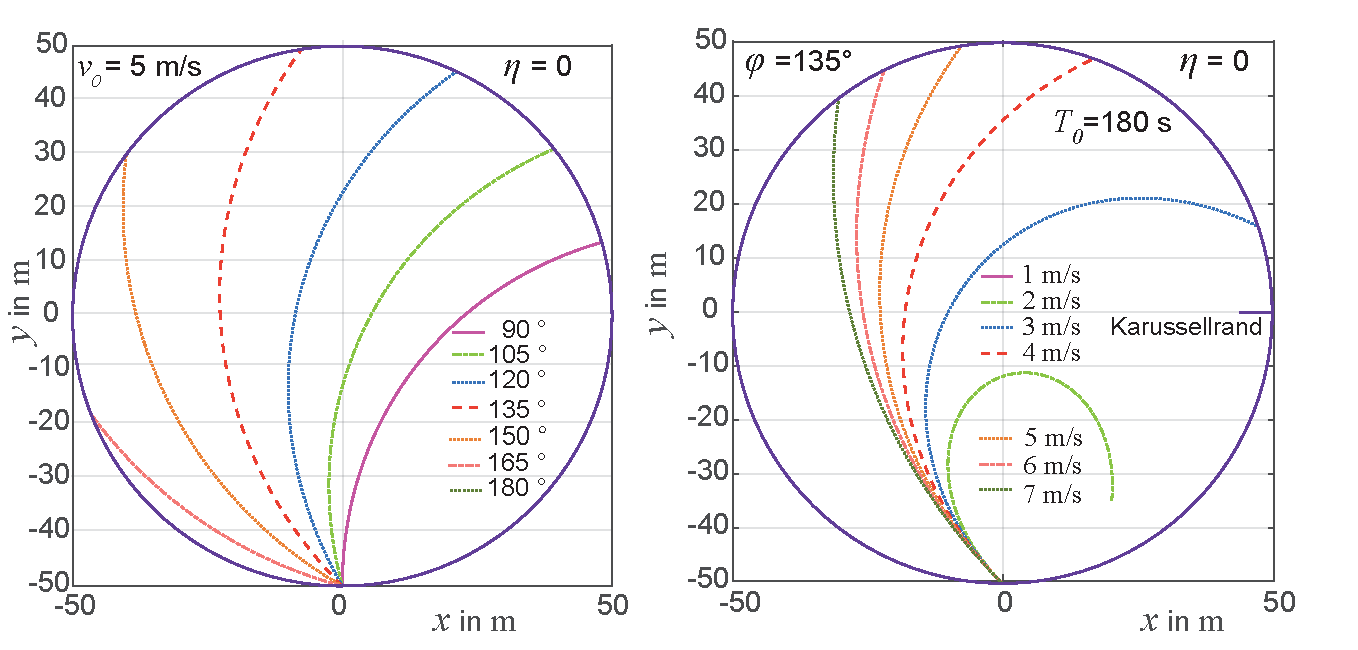
\includegraphics[width=\textwidth]{Lsg_Scheibe02.pdf}%
\caption[Trajektorien eines bewegten K�rpers auf einem  Karussell.]{Trajektorien eines bewegten K�rpers auf einem sich gleichm��ig drehenden Karussell f�r verschiedene Richtungen $\alpha$ der Anfangsgeschwindigkeit $v_0 = 5\, \mathrm{m s^{-1}}$ (Abb. links) und f�r verschiedene Anfangsgeschwindigkeiten $v_0 $ bei festgehaltener Richtung}
\label{abb:bew_Lsg_Scheibe02}
\end{figure}

\begin{figure}[H]\centering
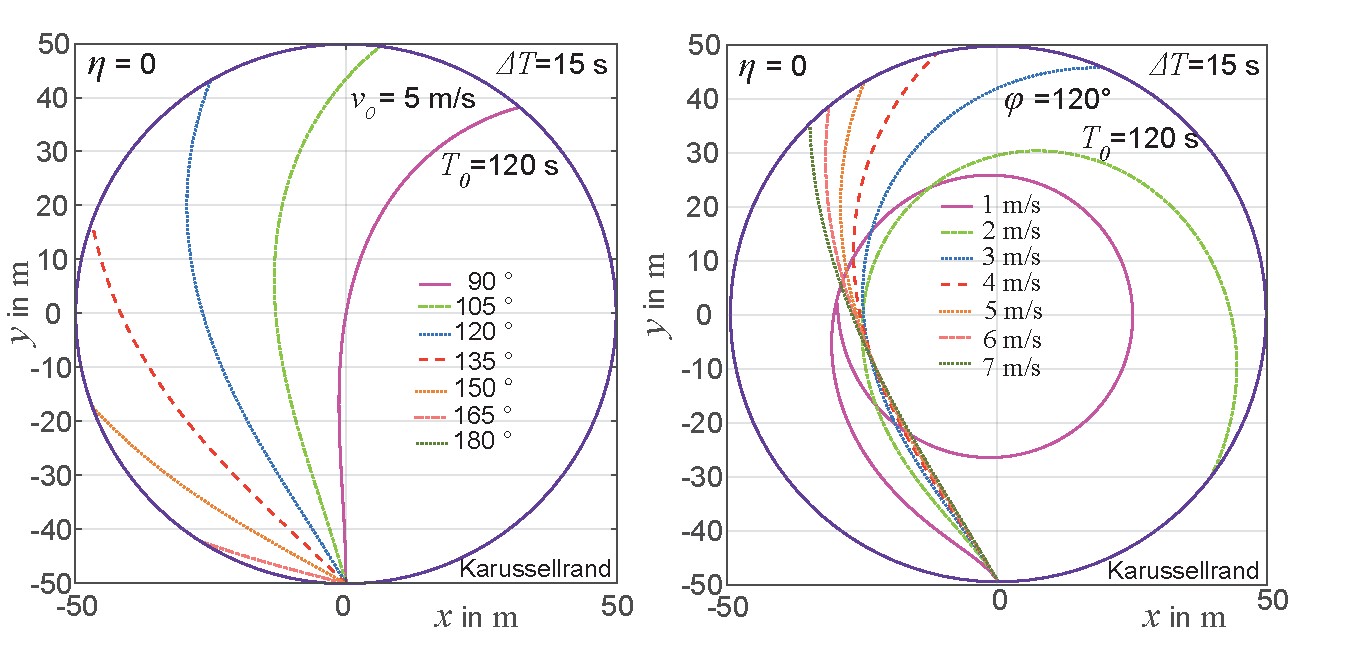
\includegraphics[width=\textwidth]{Lsg_Scheibe03.pdf}%
\caption[Trajektorien auf einem beschleunigenden Karussell]{Trajektorien eines bewegten K�rpers auf einem sich in der Rotation beschleunigenden Karussell. f�r verschiedene Richtungen $\alpha$ der Anfangsgeschwindigkeit $v_0 = 5\, \mathrm{m s^{-1}}$ (Abb. links) und f�r verschiedene Anfangsgeschwindigkeiten $v_0 $ bei festgehaltener Richtung. Das Karussell erreicht nach einer initialen Beschleunigungszeit von 15 s die dann konstante Rotationsperiode von 120 s}
\label{abb:bew_Lsg_Scheibe03}
\end{figure}

\end{subprobs}
\end{sol} 
%\href{PhysikUncut_Part1.pdf#prb:bew_Coriolis_IV}{\textcolor{blue} {$\rightarrow$ zur \probref{bew_Coriolis_IV}.}}\\
\textcolor{blue} {$\rightarrow$ zur} \probref{bew_Coriolis_IV}.\\
\noindent\rule[1ex]{\textwidth}{0.5pt}  \newpage 



%%%-----------------------------------------------------------------------------------------------------------
%%%-----------------------------------------------------------------------------------------------------------
\newpage

\subsection{�bungen zu Streuproblemen}

\medskip

%-----------------------------------------------------------------------------------------------------------
\hypertarget{lsg:bew_Rutherford}{}
\begin{sol}{prob:bew_Rutherford}\label{lsg:bew_Rutherford} %�bung22
\textbf{Rutherford-Streuung} \\ \\
Die L�sung ist im Detail in den \mscren\mlbewref{RutherfordAlpha.m} und \mlbewref{RutherfordAg.m} beschrieben.
Beispiell�sungen sind f�r $\alpha$- und Silber-Teilchen verschiedener Energien in der Laborsystem-Darstellung in \figref{bew_Rutherford02} gezeigt.

\begin{figure}[H]\centering
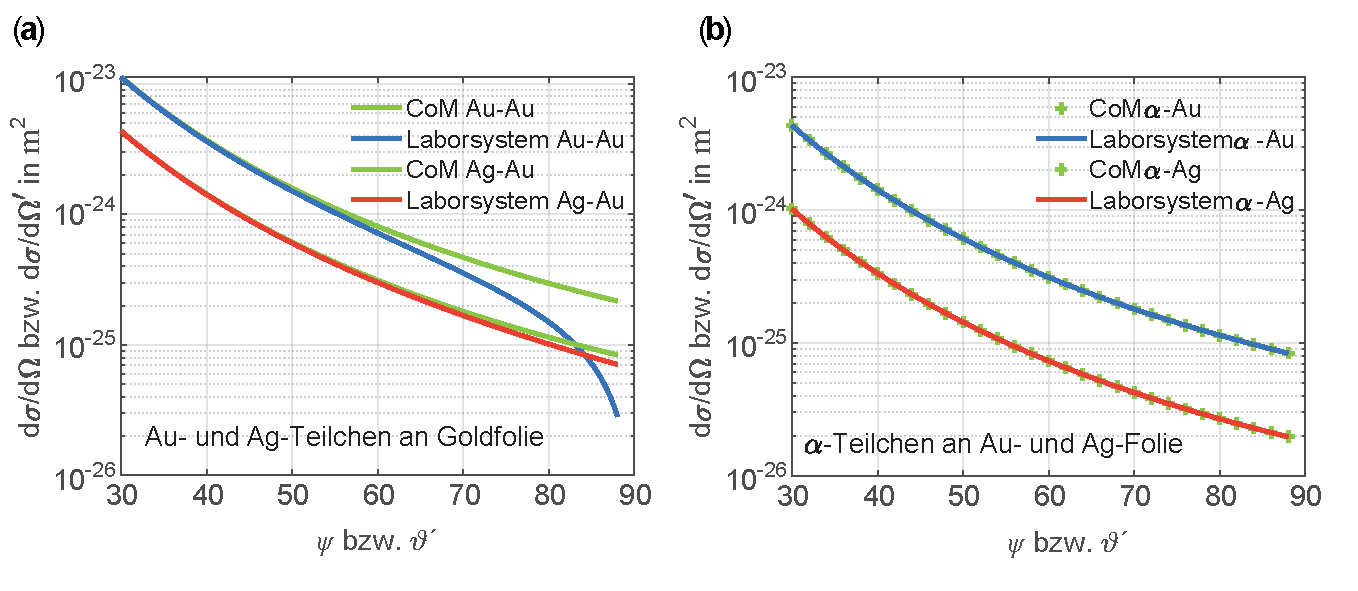
\includegraphics[width=\textwidth]{Rutherford02.pdf}
\caption[Streuung von $\alpha$- und Silber-Teilchen im Coulomb-Feld]{Streuung von \fa $\alpha$- und \fb Silber-Teilchen im Coulomb-Feld von Gold-Atomkernen f�r verschiedene Einfallsenergien (numerische Simulation). Als Ma�einheit f�r die Raumkoordinaten wurde der Bohr-Radius mit $a_\text{B} = \SI{5.29177e-11}{\metre}$ gew�hlt. Man erkennt in dieser Laborsystem-Darstellung sehr sch�n den R�cksto�effekt bei den schwereren Silberteilchen} 
\label{abb:bew_Rutherford02}
\end{figure}

\end{sol} 
%\href{PhysikUncut_Part1.pdf#prb:bew_Rutherford}{\textcolor{blue} {$\rightarrow$ zur \probref{bew_Rutherford}.}}\\
\textcolor{blue} {$\rightarrow$ zur} \probref{bew_Rutherford}.\\
\noindent\rule[1ex]{\textwidth}{0.5pt}  \newpage


%-----------------------------------------------------------------------------------------------------------
\hypertarget{lsg:bew_Asteroid}{}
\begin{sol}{prob:bew_Asteroid}\label{lsg:bew_Asteroid} %�bung23 
\textbf{Asteroiden-Auftreffwahrscheinlichkeit auf einen Planeten} \\ \\
Wir beschreiben die Bewegung der Asteroiden im KOS, dessen Nullpunkt im Zentrum des Planeten liegt (\figref{bew_astcoll01}) und betrachten nur die Gravitationswirkung des Planeten, d.\,h. wir vernachl�ssigen die Gravitation der Sonne und der anderen Planeten.\\

\begin{figure}[H]\centering
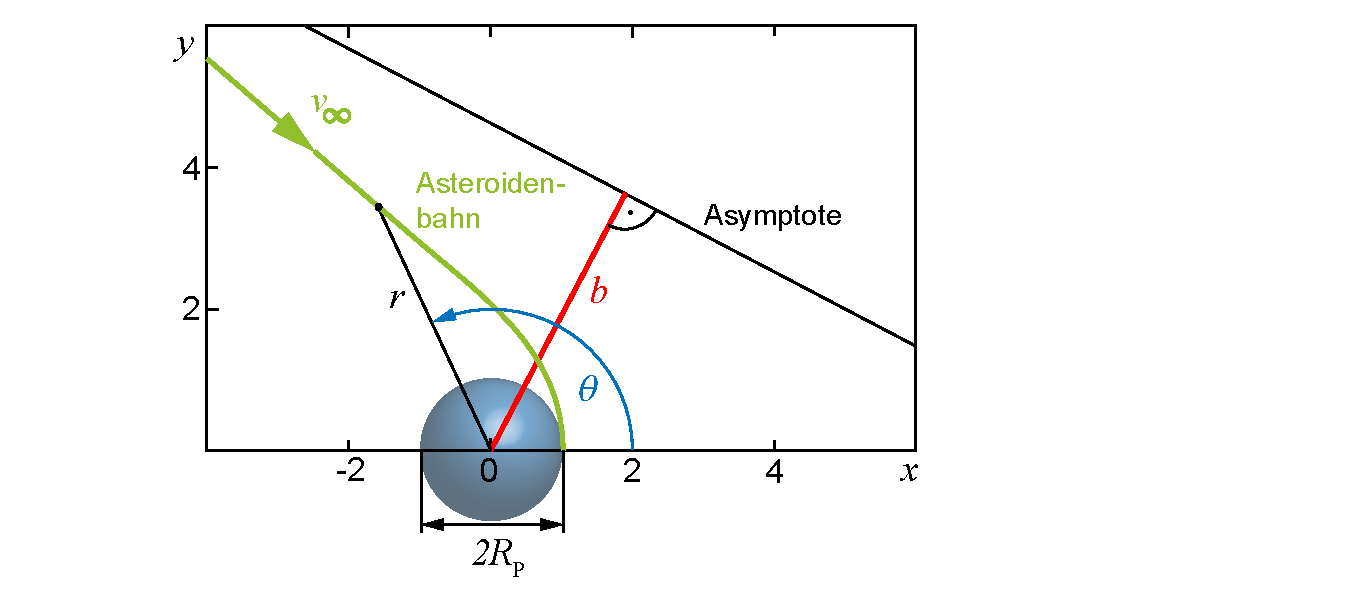
\includegraphics[width=\textwidth]{AsteroidColl01.pdf}
\caption{Streuung eines Asteroiden im Schwerefeld eines Planeten} 
\label{abb:bew_astcoll01}
\end{figure}

Der spezifische (auf die Masse bezogene) Drehimpuls ($L \equiv L/m$) des Asteroiden gegen�ber dem Planetenzentrum ist 
        \begin{align}
            L = v_\infty \,b \,, \label{eq:bew_astcoll01}
        \end{align}
worin $v_\infty$ die Geschwindigkeit des Asteroiden weit ab vom Planeten ist. Die spezifische (wiederum auf die Masse bezogene) Energie ($E \equiv E(r)/m$) des Asteroiden Energie im $\infty$ ist $E_\infty=\frac{m}{2}\,{v_\infty}^2$, so dass 
        \begin{align*}
            E(r) = -\frac{G\,m_\text{P}}{r} + \frac{1}{2}\,\lek v\lk r\rk\rek^2 = E_\infty = \frac{1}{2}\,{v_\infty}^2\,,
        \end{align*}
woraus die Energie im Abstand $r$
        \begin{align}
            \lek v\lk r\rk\rek^2 = {v_\infty}^2 + \frac{2G\,m_\text{P}}{r} \label{eq:bew_astcoll02}
        \end{align}
folgt. Wir haben dabei die auf die Masse $m$ des Asteroiden bezogenen Gr��en verwendet. \\
In diesem Streuproblem bewegt sich der Asteroid nach \eqref{eq:bew_Bahn_explizit} auf einer Hyperbelbahn:
        \begin{align}
            r = \frac{L^2}{G\,m_\text{P}}\, \frac{1}{1+e\,\cos\theta}\,, \label{eq:bew_astcoll03}
        \end{align}
deren Exzentrizit�t $\epsilon$ durch \eqref{eq:bew_Bahn_Exzentrizitaet} 
        \begin{align}
            \epsilon = \sqrt{1+\frac{2\,E\,L^2}{\lk G\,m_\text{P}\rk^2}} = \sqrt{1+\frac{{v_\infty}^4 b^2} {\lk G\,m_\text{P}\rk^2}} \label{eq:bew_astcoll04}
        \end{align}
gegeben ist. Der minimale Abstand wird bei $r_\text{min}\lk\theta = 0 \rk$ erreicht, also bei\\
$L^2/\lk G\,M\rk = r_\text{min}\lk 1+\epsilon\rk$,\\
so dass wir f�r \eqref{eq:bew_astcoll03} schreiben k�nnen:
        \begin{align}
            r\lk \theta\rk = \frac{r_\text{min}\lk 1+\epsilon\rk}{1+\epsilon\,\cos\theta}\,. \label{eq:bew_astcoll05}
        \end{align}
Ferner gilt f�r die Hyperbel die Beziehung \eqref{eq:bew_hyp_asymptote}) woraus man
        \begin{align*}
            b = r_\text{min}\,\sqrt{\frac{\epsilon+1}{\epsilon-1}}1\,
        \end{align*}
herleiten kann. Abh�ngig von den Parametern $m_\text{P}$, $v_\infty$ und $b$ und dem Radius $R_\text{P}$ kann es unter Umst�nden zu einer Kollision kommen, und zwar dann wenn $r_\text{min}\leq R_\text{P}$ bzw. 
	\[\frac{r_\text{min}}{R_\text{P}} = \frac{b}{R_\text{P} \sqrt{\frac{\epsilon-1}{\epsilon+1}} < 1} \,.
	\]
	Durch die Gravitation ist der Streuquerschnitt der Kollision um einen Faktor $\gamma$ gr��er als rein geometrisch gegeben, 
        \begin{align}
            \gamma = \frac{\pi\,b^2}{\pi\,{R_\text{P}}^2} = \lk \frac{b}{R_\text{P}} \rk^2 \,. \label{eq:bew_astcoll07}
        \end{align}
Beim Erreichen des minimalen Abstands $r_\text{min} = R_\text{P}$ zum Planeten hat der Asteroid folgende Energie
        \begin{align*}
            {v_\infty}^2 +\frac{2G\,m_\text{P}}{R_\text{P}} = v\lk r_\text{min}\rk^2 = {v_\text{r,min}}^2\,.
         \end{align*}
Ferner gilt Drehimpulserhaltung: $ v_\infty\,b = v_\text{r,min}\,R_\text{P} \,.$
Wir ersetzen $v_\text{r,min}$ und erhalten: 
        \begin{align*}
            {v_\infty}^2 + \frac{2G\,m_\text{P}}{R_\text{P}} = \lk \frac{b}{R}\rk^2\,{v_\infty}^2\,.
        \end{align*}
Das kann man schreiben als 
        \begin{align}
            \gamma = 1 + \frac{\lk \sqrt{\frac{2G\,m_\text{P}}{R_\text{P}}}\rk^2}{{v_\infty}^2} = 1+\lk \frac{v_\text{F}}{v_\infty}\rk^2 \,, \label{eq:bew_astcoll08}
        \end{align}
worin $v_\text{F}$ die sogenannte \gls{vescape} vom jeweiligen Planeten ist. Gleichung \eqref{eq:bew_astcoll08} besagt also, dass der Kollisionsquerschnitt umso gr��er ist, je gr��er die Fluchtgeschwindigkeit und je kleiner die \glqq Einfallsgeschwindigkeit \grqq{} $v_\infty$ des Asteroiden ist (Tabelle \ref{tab:bew_astcoll01}).

\begin{table}[h!]
\centering
\begin{tabular}{|L{1.2cm}|C{2cm}|C{2cm}|C{2cm}|}
\hline
%\rule{0pt}{3pt}& & &   \\
  & $R_\text{P}$  & $v_\text{esc}$ & $\gamma$ \\
\rule{0pt}{3pt}& km & km/s &  \\
\hline
%\rule{0pt}{3pt}& & &  \\
\rule{0pt}{6pt}Erde   & $\SI{6378}{}$ & $\SI{11.2}{}$ & $\SI{2.25}{}$  \\
\rule{0pt}{6pt}Mars & $\SI{3397}{}$  & $\SI{5.0}{}$ & $\SI{1.25}{}$ \\
\rule{0pt}{6pt}Jupiter  & $\SI{71492}{}$ & $\SI{59.5}{}$ & $\SI{36.45}{}$ \\
%\rule{0pt}{3pt}& & &  \\
\hline
\end{tabular}
\smallskip
\caption{Berechnete Werte f�r Asteroideneinfall auf verschiedene Planeten} \label{tab:bew_astcoll01}
\end{table}
\figref{bew_astcoll02} zeigt Trajektorien von parallel einfallenden Asteroiden aber unterschiedlichen Sto�parametern f�r die Planeten Jupiter und Erde in Einheiten des Radius des jeweiligen Planeten.
Die Einfallsgeschwindigkeit wurde in beiden F�llen zu $\SI{14.0}{\km\per\s}$ angenommen.
Man erkennt, dass der Jupiter wie erwartet einen deutlich gr��eren Kollisionsquerschnitt hat.
Zur Vertiefung empfehlen wir \mlbewref{AsteroidKollision.m}, \mlbewref{AsteroidStreuung.m} und \cite{VanAllen2006}.
\begin{figure}[H]\centering
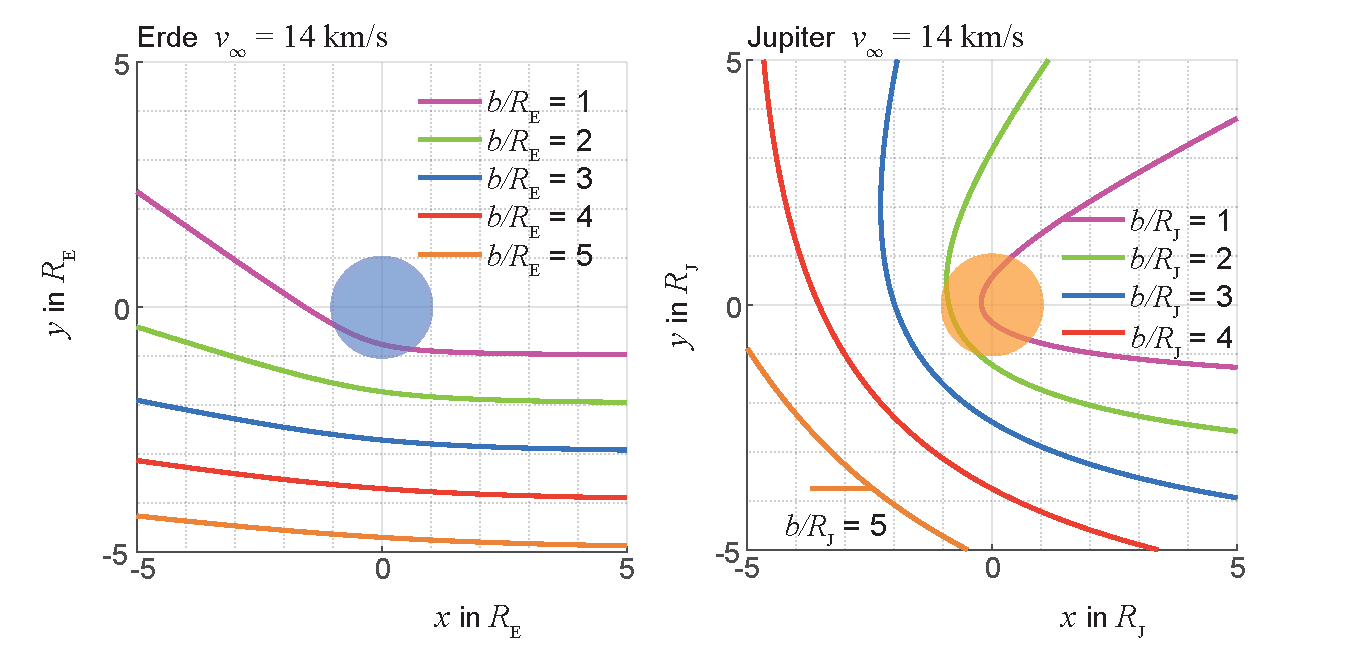
\includegraphics[width=\textwidth]{AsteroidColl02.pdf}
\caption[Trajektorien von einfallenden Asteroiden f�r Jupiter und Erde]{Trajektorien von einfallenden Asteroiden f�r Jupiter und Erde in Einheiten des Radius des jeweiligen Planeten} 
\label{abb:bew_astcoll02}
\end{figure}

\smallskip
\end{sol} 
%\href{PhysikUncut_Part1.pdf#prb:bew_Asteroid}{\textcolor{blue} {$\rightarrow$ zur \probref{bew_Asteroid}.}}\\
\textcolor{blue} {$\rightarrow$ zur} \probref{bew_Asteroid}.\\
\noindent\rule[1ex]{\textwidth}{0.5pt}  \newpage


%%%-----------------------------------------------------------------------------------------------------------
%%%-----------------------------------------------------------------------------------------------------------
\newpage

\subsection{�bungen zu Oszillatoren und Pendel}

\medskip
%-----------------------------------------------------------------------------------------------------------
\hypertarget{lsg:bew_PendelGl}{}
\begin{sol}{prob:bew_PendelGl}\label{lsg:bew_PendelGl} %�bung24
\textbf{Pendelgleichungen} \\ \\
Wir starten von \eqref{eq:bew_Schwingung01b} und betrachten ein Pendel mit der Fadenl�nge $l$, an dem eine Masse $m$ aufgeh�ngt ist.
Die generalisierte Koordinate ist der Winkel $\varphi$. 
Aus $x = l \sin\varphi$ und $z = -l \cos\varphi$ folgt 
\begin{align*}
		h\lk \varphi \rk &= \lk \frac{\d x}{\d \varphi} \rk^2 + \lk \frac{\d z}{\d \varphi} \rk^2 = l^2 \,, \\
		U \lk \varphi \rk &= -m g l \cos\varphi \,, \\
		&= -m g l\,\lk 1-\frac{1}{2}\cos^2\varphi\, \big|_{\varphi=0}\,\varphi^2+\frac{1}{24} \cos^4\varphi \,\big|_{\varphi=0}\, \varphi^4 + \sum_k \frac{\lk -1 \rk^k}{\lk 2k \rk !}\varphi^{2k}\rk.
\end{align*}
Hierbei haben wir im Potential nur die von Null verschiedenen Terme mitgenommen, den ersten Term $-m\,g\,l$ k�nnen wir ohne weiteres \anf{wegeichen}.
Da bei dem Pendel $h\lk \varphi \rk = \text{const} = l^2$ ist, gilt f�r die Bewegungsgleichung
\begin{align}
		m\,\frac{\D}{\D t}\lk l^2\,\dot{\varphi}\rk + \frac{\d U\lk \varphi \rk}{\d \varphi} &= 0 \,, \\
		m\,l^2\,\ddot{\varphi} + m\,g\,l\,\frac{\d}{\d \varphi} \lk \frac{1}{2} \varphi^2-\frac{1}{24} \varphi^4 + \sum_k \frac{\lk -1 \rk^k}{\lk 2k \rk !}\varphi^{2k}\rk &= 0 \,, \\
		\ddot{\varphi} + \frac{g}{l} \lk \varphi - \frac{1}{6} \varphi^3 + \sum_k \frac{\lk -1 \rk^k}{\lk 2k-1 \rk !}\varphi^{2k-1}\rk &= 0 \,.
\end{align}
Wir haben also die Bewegungsgleichung des Pendels als Reihe aufschreiben k�nnen.
Dies legt nahe, dass wir auch die Schwingungsperiode $T_\text{P} = 2\pi\sqrt{\frac{l}{g}}$ als Reihe entwickeln k�nnen.


\end{sol} 
%\href{PhysikUncut_Part1.pdf#prb:bew_PendelGl}{\textcolor{blue} {$\rightarrow$ zur \probref{bew_PendelGl}.}}\\
\textcolor{blue} {$\rightarrow$ zur} \probref{bew_PendelGl}.\\
\noindent\rule[1ex]{\textwidth}{0.5pt}  \newpage


%-----------------------------------------------------------------------------------------------------------
\hypertarget{lsg:bew_HO_quadrat}{}
\begin{sol}{prob:bew_HO_quadrat}\label{lsg:bew_HO_quadrat} %�bung25
\textbf{Harmonischer Oszillator mit quadratischem Reibungsterm.} \\

Die Bewegungsgleichungen lauten f�r den (eindimensionalen) harmonischer Oszillator mit quadratischem Reibungsterm (Newton-Reibung):
\begin{align}
			m\,\ddot{q} &= - m\,{\omega_0}^2\,q  - m \, \eta_\text{N}\,\mathrm{sign}(\dot{q})\,\dot{q}^2 \,. \label{eq:bew_HO_quadfriction01}
\end{align}
Es ist zu beachten, dass der Reibungsterm das Vorzeichen jedes mal wechselt, wenn $\dot{q}=0$, \dh zweimal pro voller Schwingung.
Dies wird durch die Signum-Funktion ber�cksichtigt und muss bei der \matlab{} Programmierung entsprechend beachtet werden.
Diese ist in \mlbewref{HarmonOszQuadReibung.m} ausgef�hrt.
Zur Erinnerung die Bewegungsgleichung des harmonischen Oszillator mit linearem Reibungsterm (Stokes-Reibung) \eqref{eq:bew_pendulum02}:
\begin{align}
			m\,\ddot{q} &= - m\,{\omega_0}^2\,x  - m \, \eta_\text{S}\,\dot{q} \,. \label{eq:bew_HO_quadfriction02}
\end{align}
Das Ergebnis der Integration der beiden Bewegungsgleichungen ist im Vergleich zum unged�mpften Fall in \figref{bew_HO_quadrat01} zu sehen, \figref{bew_HO_quadrat02} zeigt die Energieabnahme des jeweiligen Oszillators �ber die Zeit.
\begin{figure}[H]\centering
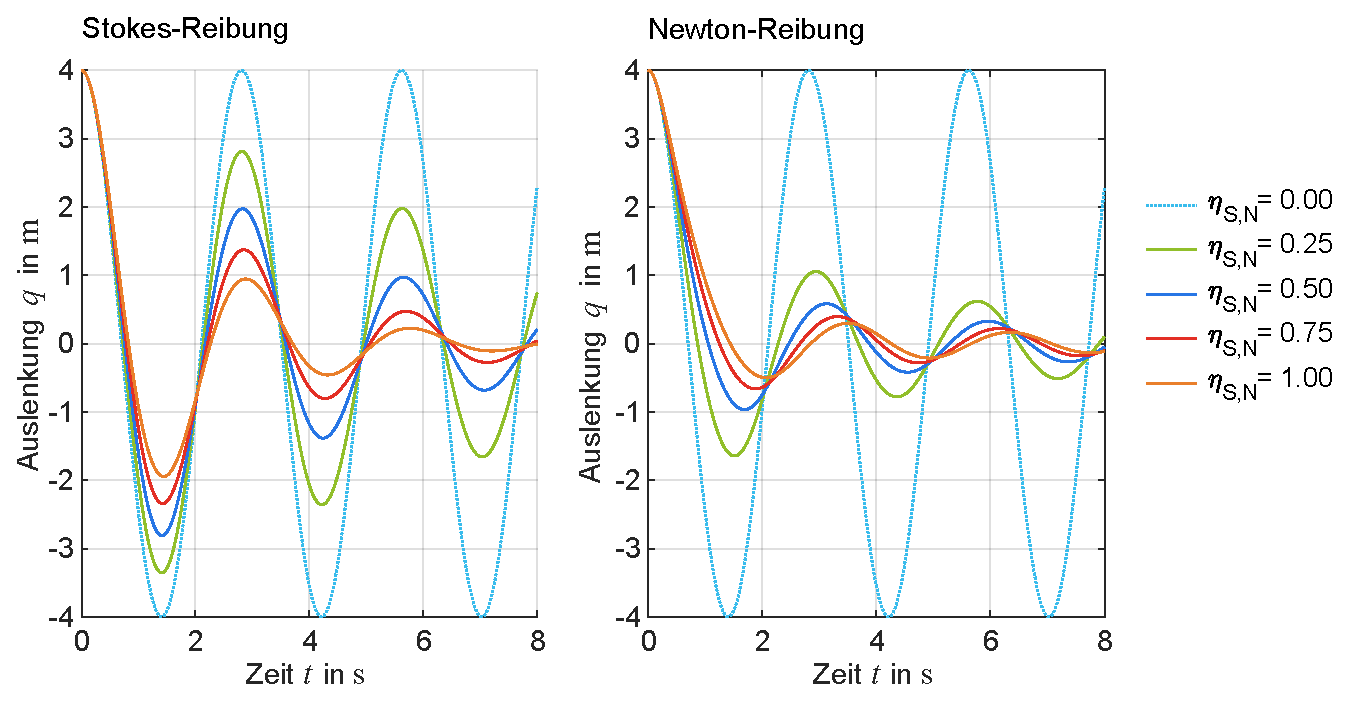
\includegraphics[width=\textwidth]{HO_Quadrat01.pdf}%
\caption[L�sung der Bewegungsgleichung f�r den harmonischer Oszillator]{Vergleich der L�sungen der Bewegungsgleichung f�r den harmonischer Oszillator mit quadratischen Reibungsterm (Newton-Reibung) (rechts) und linearem Reibungsterm (Stokes-Reibung) f�r verschiedene Parameter (links)}
\label{abb:bew_HO_quadrat01}
\end{figure}
\begin{figure}[H]\centering
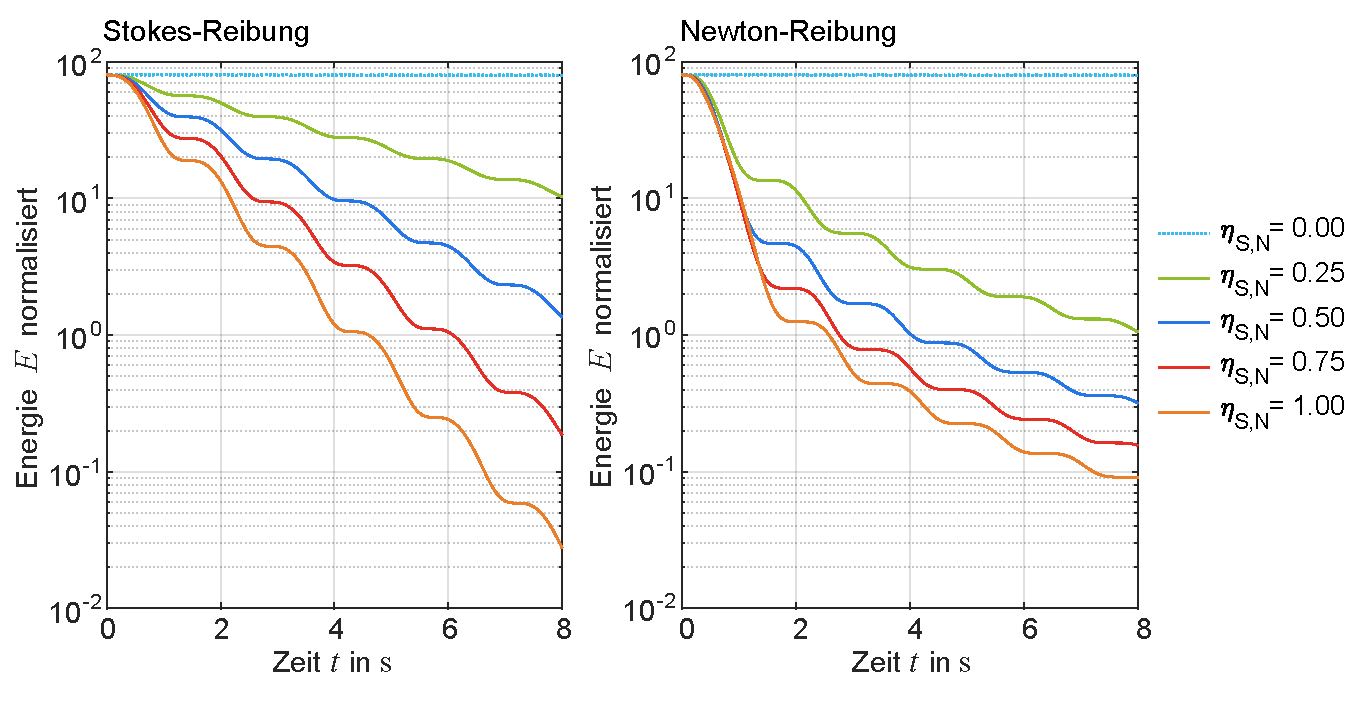
\includegraphics[width=\textwidth]{HO_Quadrat02.pdf}%
\caption[Energiedissipation des harmonischen Oszillators]{Energiedissipation des harmonischen Oszillators mit quadratischen Reibungsterm (Newton-Reibung) f�r verschiedene Parameter (rechts) und im Vergleich zur Energiedissipation beim Oszillator mit Stokes-Reibung (links)}
\label{abb:bew_HO_quadrat02}
\end{figure}

Man erkennt, dass beim harmonischen Oszillator mit quadratischem Reibungsterm die Frequenz $\omega$ wie auch die Energieabnahme stark von den Anfangsbedingungen abh�ngen. Die Schwingungsperiode $T_P$ ist dar�ber hinaus stark von der Eigenfrequenz $T_{P0}=2\pi/\omega_0$ verschieden und auch noch von der Zeit abh�ngig. Die Energiedissipation beim harmonischen Oszillator passiert zu Beginn viel schneller. Ist aber ein niedriges Niveau erreicht, dann dissipiert die Energie des Systems deutlich langsamer als im linearen Reibungsfall. 
F�r interessierte Leser sei die relativ komplizierte analytische L�sung in \cite{Smith2012} zur Lekt�re empfohlen.
\end{sol} 
%\href{PhysikUncut_Part1.pdf#prb:bew_HO_quadrat}{\textcolor{blue} {$\rightarrow$ zur \probref{bew_HO_quadrat}.}}\\
\textcolor{blue} {$\rightarrow$ zur} \probref{bew_HO_quadrat}.\\
\noindent\rule[1ex]{\textwidth}{0.5pt}  \newpage


%-----------------------------------------------------------------------------------------------------------
\hypertarget{lsg:bew_ExamplesHO}{}
\begin{sol}{prob:bew_ExamplesHO}\label{lsg:bew_ExamplesHO} %�bung26
\textbf{Beispiele f�r harmonische Schwingungen (\vgl auch \cite{Hasbun2018}.).} 

\begin{figure}[H]\centering
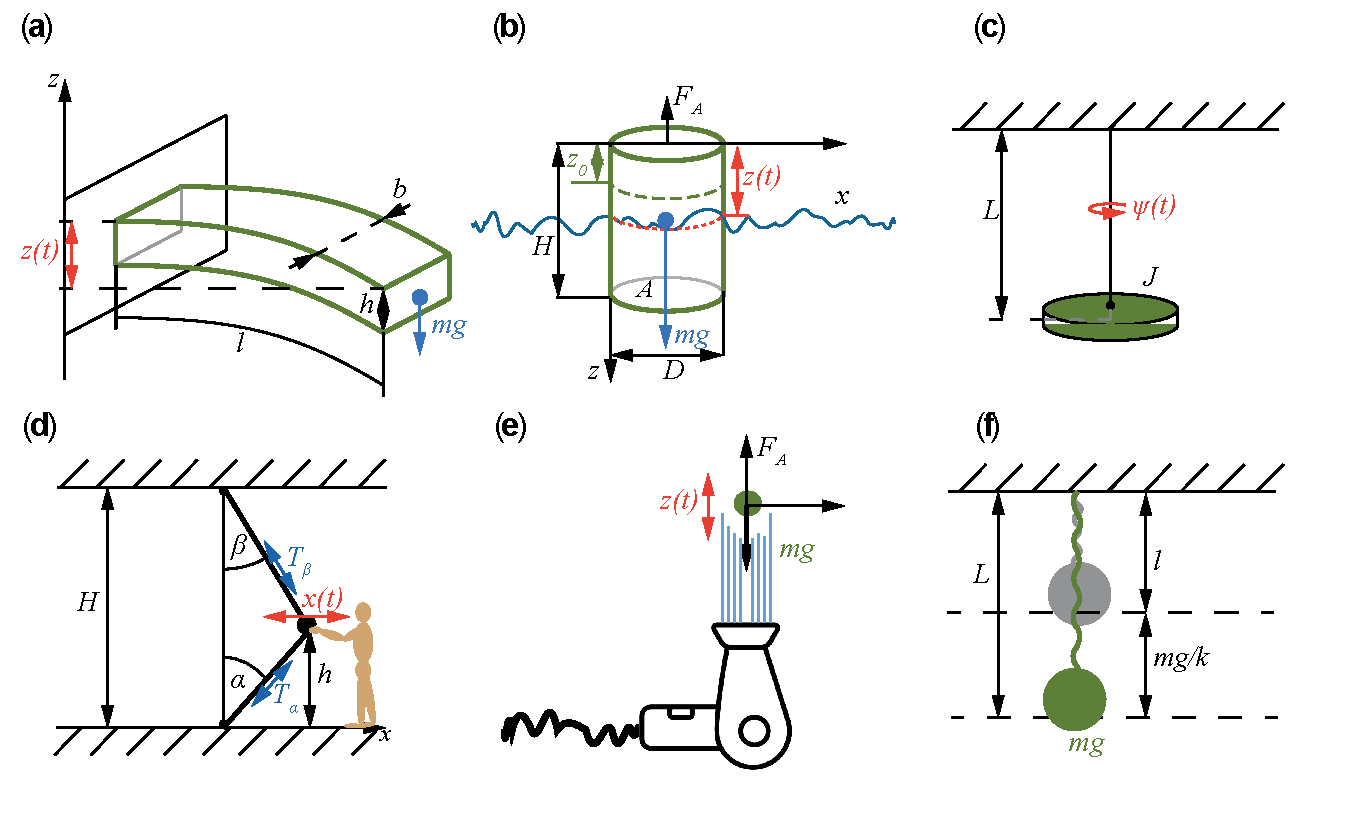
\includegraphics[width=\textwidth]{BeispieleHO.pdf}
\caption[Beispiele f�r harmonische Schwingungen]{Beispiele f�r harmonische Schwingungen} 
\label{abb:bew_HOex02}
\end{figure}

\begin{subprobs}
\subprob{Sprungbrett (\figref{bew_HOex02}\,a)}
Wir werden im Kapitel Kontinuumsmechanik (\ref{chap:kontmech}) sehen, dass die Auslenkung $z$ eines Balkens bei einer wirkenden Kraft $F$ gegeben ist durch:
	\begin{align*}
			 z = -\frac{L^3\, 12}{3Y\,b\,h^3}\,F = -4\,\frac{l^3}{b\,h^3}\,\frac{F}{Y}\,.
	\end{align*}
Hierin sind $Y$ der Young-Elastizit�tsmodul\footnote{Thomas Young\indexp{Young, Thomas} (1773--1829) war ein englischer Augenarzt und Physiker. Young forschte zur Wellennatur und insbesondere zur Interferenz des Lichts. Ber�hmt ist sein Doppelspaltexperiment, welches sp�ter f�r die Entwicklung der Quantenmechanik eine wichtige Rolle spielte.}
und $l,b,h$ die L�nge, Breite \bzw H�he des Balkens.
Wir haben also $z \propto F$. \\
Wenn man jetzt die Kraft am Ende des Balkens durch eine fest angebrachte Masse  $m=\SI{100}{\kg}$ hervor gebracht denkt, dann ist die Gleichgewichtslage durch 
\[z_0 = -\frac{4L^3}{b\,h^3}\frac{m\,g}{Y}\]
gegeben. 
Der Balken kann dann als schwingendes System um die neue Gleichgewichtslage betrachtet werden.
Die Bewegungsgleichung f�r die am Balkenende befestigte Masse $m$ lautet: 
		\begin{align}
				m\,\ddot{z} = -\frac{Y\,b\,h^3}{4L^3}\lk z-z_0\rk \,. \label{eq:bew_HOexL01}
		\end{align}

\newpage
Die Schwingungsfrequenz	ist gegeben durch
		\begin{align*}
				\omega = \sqrt{\frac{Y\,b\,h^3}{4m\,l^3}}\,.
		\end{align*}
Ein typisches Sprungbrett mit $l = \SI{5}{\metre}$, $h = \SI{10}{\cm}$ und $b = \SI{1}{\metre}$ aus Holz mit dem Elastizit�tsmodul $Y = \SI{1e09}{\newton\per\square\metre}$ hat also eine Schwingungsperiode von etwa $T_\text{P}=2\pi/\omega=\SI{1.4}{\second}$. \\ %Masse war nicht gegeben

\subprob{Tonne im Wasser (\figref{bew_HOex02}\,b)} \\
Im Gleichgewicht entspricht der Auftrieb dem verdr�ngtem Wassergewicht, also
		\begin{align*}
				F_\text{A0} = \varrho_\text{W} A \,\lk H-z_0 \rk g = m \,g \,,
		\end{align*}
woraus
		\begin{align*}
				z_0 = H-\frac{m}{\varrho_\text{W}A} 
		\end{align*}
folgt. 
Kommt es zu einer kleinen Verschiebung $\Delta z = z-z_0$ aus der Gleichgewichtslage, so ver�ndert sich auch die Auftriebskraft:
		\begin{align*}
				\Delta F = F_\text{A} -F_\text{A0} = \varrho_\text{W}\,A\,g\,\lek\lk H-z\rk-\lk H-z_0\rk\rek\,.
		\end{align*}
Aus dem zweiten Newtonschen Axiom folgt dann f�r die Tonnenh�he oberhalb des Wassers $z$:
		\begin{align*}
				m \,\ddot{z} &= F_\text{A}(z)-m\,g = F_\text{A}(z) -F_\text{A0}(z_0) \,,\\
				m \,\ddot{z} &= \varrho_\text{W}\,g\,A\lk z-z_0\rk \,.
		\end{align*}
Wir setzen $z-z_0 = +\,\xi$ bei $z_0<0$ und erhalten
		\begin{align*}
				\ddot{\xi} &= -\frac{\varrho_\text{W}\,g\,A}{m} \xi \,, \\
				\omega &= \sqrt{\frac{\varrho_\text{W}\,g\,A}{m}} \,.
		\end{align*}
Die Tonne schwingt also umso heftiger je geringer Ihre Masse ist und je gr��er ihr Durchmesser.

\subprob{Torsionspendel (\figref{bew_HOex02}\,c)}
Man kann die Bewegungsgleichung der linearen Feder in Analogie auf das Torsionspendel �bertragen.
D.h. die Parameter Masse $m$, Federkonstante $k$ und Auslenkung $x$ einer linearen Feder entsprechen den Parametern Tr�gheitsmoment $J$ (Einheit $\SI{}{\kg\square\meter}$), Direktionsmoment $D$ (Einheit  $ \SI{}{\newton\meter\per\radian}$) und Auslenkungswinkel $\varphi$ (Einheit $ \SI{}{\radian} $). 
Das Direktionsmoment ist -- wie auch die Federkonstante -- eine Materialeigenschaft des Drahtes. 
Damit lautet die Bewegungsgleichung $J\,\ddot{\varphi} + D\,\varphi = 0$, wobei $J$ auf die Achse bezogen ist, die durch die Aufh�ngung gegeben ist. 
F�r einen Draht mit Radius $r_\text{D}$ und L�nge $L$ (ohne Scheibe) gilt:
		\begin{align*}
				D = \frac{\pi r_\text{D}^4}{2}\frac{G_\text{S}}{L} \,.
		\end{align*}
Die Gr��e $G_\text{S}$ ist dabei das Schubmodul, welches wiederum mit der Poissonzahl\index{Poissonzahl}\footnote{Sim�on Denis Poisson (1781--1840 in Paris) war ein franz�sischer Physiker und Mathematiker. Er war Sch�ler von Laplace und besch�ftigte sich vor allem mit der Theorie der Wellen in der Akustik, der Elastizit�ts- und W�rmelehre, sowie der Potentialtheorie der Elektrostatik. Als Mathematiker arbeitete Poisson vor allem auf den Gebieten der Differentialgeometrie, der Infinitesimal- und Wahrscheinlichkeitsrechnung. Mehrere mathematische Begriffe sind mit seinem Namen verbunden. Er war sehr produktiv und ver�ffentlichte insgesamt �ber 300 Arbeiten.}\indexp{Poisson, Sim�on Denis} $\mu$ (ein Wert zwischen 0 und 0.5) �ber $G_\text{S} = \frac{1}{2(1+\mu)}\,Y$ direkt proportional zum Elastizit�tsmodul $Y$ ist. 
Die Frequenz ergibt sich dann zu 
		\begin{align*}
				\omega = \sqrt{\frac{D}{J}} \,.
		\end{align*}
F�r eine zentrisch aufgeh�ngte Scheibe gilt $J = \frac{1}{2}m_\text{s}R_\text{s}^2$ und damit erh�lt man
		\begin{align*}
				\omega = \frac{r_\text{D}^2}{R_\text{s}}\sqrt{\frac{G_\text{S}}{L}\frac{\pi}{m_\text{s}}}
		\end{align*}
f�r die Kreisfrequenz. \\
Torsionspendel haben in der Zeitmessung eine gro�e Rolle gespielt.
Das liegt vor allem daran, dass der Zusammenhang zwischen dem r�cktreibenden Moment $D_\varphi$ und der Auslenkung $\varphi$ im Gegensatz zum mathematischen Pendel oder der linearen Feder nicht nur f�r kleine Winkel linear ist.

\subprob{Zugseil im Fitnessstudio (\figref{bew_HOex02}\,d)}
Aus der \figref{bew_HOex02}d k�nnen wir die Spannung im Seil in guter N�herung f�r kleine Winkel $\alpha$ und $\beta$ als konstant ansehen, also $T = T_\alpha = T_\beta$.
Aus der Geometrie in der Abb. folgt somit f�r die $x$-Komponente der Seilspannung als r�cktreibende Kraft:
		\begin{align*}
					m\,\ddot{x} &= -T_\alpha\sin\!\alpha(t)-T_\beta\sin\!\beta(t) = -T\, \lk \frac{x}{\sqrt{x^2+h^2}}+\frac{x}{\sqrt{x^2+\lk H-h\rk ^2}}\rk \,.
		\end{align*}
F�r $x \ll h$ gilt die N�herung	
	\begin{align*}
			m\,\ddot{x} &\approx - T \, \lk\frac{x}{h}+\frac{x}{H-h}-\mathcal{O}(x^3)\rk\\
			\rightarrow m\,\ddot{x} &= - \frac{T\,H}{h\lk H-h\rk}\,x  \\
			\rightarrow \omega &= \sqrt{\frac{T}{m}\frac{H}{h\lk H-h\rk}}\,.
	\end{align*}
F�r $h = \frac{H}{2}$ folgt:
	\begin{align*}
			&m\,\ddot{x} + 4\,\frac{T}{H}\,x = 0 \,, \\
			\rightarrow \omega &= \sqrt{\frac{4T}{m\,H}} 
			\qquad \text{with} \quad m = \varrho^\text{(L)}H \\
			&= \sqrt{\frac{4T}{\varrho^\text{(L)}H^2}} 
			= \frac{2}{H}\sqrt{\frac{T}{\varrho^\text{L}}}\,.
	\end{align*}
Man �berlege sich, was dieser Ausdruck physikalisch bedeutet.
Hinweis: $f = {\omega}/{2\pi}= {c_\text{ph}}/{\lambda}$. \\

\subprob{Tischtennisball im F�n (\figref{bew_HOex02}\,e)}
Wir werden in der Mechanik der Kontinua (\autoref{chap:kontmech}) die Bernoulli%
\footnote{Daniel Bernoulli\indexp{Bernoulli, Daniel} (1700--1782) war ein Schweizer Mathematiker und Physiker aus der Gelehrtenfamilie der Bernoullis. Er arbeitete auf vielen Gebieten u.a. mit Leonhard Euler. Die nach ihm benannte Bernoulli-Gleichung ist von zentraler Bedeutung in der Hydro- und Aerodynamik.}-Gleichung kennenlernen,
die den Fluss laminarer, nichtkompressibler Fl�ssigkeiten und Gase beschreibt. 
Die Str�mungsgeschwindigkeit des Luftstroms sei $v(z)$, die Masse des Tischtennisballs $m$ und die Bewegungskoordinate $z$. 
Beim Austritt aus dem F�n gelte $v(z=0) = v_\text{A}$. 
Dann gilt f�r die Geschwindigkeit $v_\text{A}$ der Luftmolek�le nach der Bernoulli-Gleichung%
\footnote{Man kann die Bernoulli-Gleichung auch als Energieerhaltung von spezifischer kinetischer und potentieller Energie deuten.}:
		\begin{align*}
				\frac{1}{2} \varrho\,{v_\text{A}}^2 &= \frac{1}{2} \varrho\,v(z)^2+\varrho\,g\,z \,, \\
				\rightarrow v(z) &= v_\text{A} \sqrt{1-\frac{2g\,z}{{v_\text{A}}^2}} \approx v_\text{A} \lk 1-\frac{g\,z}{{v_\text{A}}^2}\rk \,.
		\end{align*}
Auf den Tischtennisball wirkt die Gewichtskraft und die (Stokes-)Reibungskraft, also gilt:
		\begin{align*}
				F=m\,\ddot{z} &= -m\,g+\eta\,v(z) \,, \\
				\rightarrow m\,\ddot{z} &= -m\,g + \eta\,v_\text{A} \lk 1 -\frac{g\,z}{{v_\text{A}}^2} \rk \,.
		\end{align*}
Im Gleichgewicht $z=z_0$ muss $F=-m\,g+\eta\,v(z_0) = 0$ sein, woraus folgt:
		\begin{align*}
				v(z_0) &= \frac{m\,g}{\eta} = v_\text{A}\lk 1-\frac{g\,z_0}{{v_\text{A}}^2}\rk ~~ \text{und daher} \\
				z_0 &= v_\text{A} \lk \frac{v_\text{A}}{g}-\frac{m}{\eta}\rk.
		\end{align*}
Somit lautet die Bewegungsgleichung und die entsprechende Frequenz
		\begin{align*}
				\ddot{z} + \frac{\eta\,g}{m\,v_\text{A}}\lk z-z_0\rk = 0 
				\quad \text{mit} \quad 
				\omega = \sqrt{\frac{\eta\,g}{m\,v_\text{A}}}\,.
		\end{align*}
Interessanterweise ist die Frequenz der Schwingung umso gr��er, je gr��er die D�mpfung $\eta$ (z.B. durch Reibung und/oder Viskosit�t) und umso kleiner die Austrittsgeschwindigkeit $v_\text{A}$ des Luftstromes ist.

\subprob{Feder mit Masse und ver�nderter Gleichgewichtslage (\figref{bew_HOex02}\,f)}
Aus der \figref{bew_HOex02}\,f k�nnen wir die Bewegungsgleichung bei ver�nderter Gleichgewichtslage direkt aufschreiben:
		\begin{align*}
				\ddot{z} +\omega^2 \lk z - z_\text{G}\rk = 0 \,.
		\end{align*}
Die Gleichung hat eine �hnliche Struktur und damit die gleiche L�sung wie \eqref{eq:bew_pendulum01}.
Allerdings sind die Konstanten der L�sung wegen der anderen Anfangsbedingungen neu zu bestimmen.
Wir schreiben die L�sung als
		\begin{align*}
				z &= z_\text{G} + A\sin\lk \omega t+\varphi\rk\,. \\
		\end{align*}
Mit $\dot{z} = A\, \omega\cos\lk \omega t+ \varphi\rk$ und \obda f�r $\varphi=0$ f�r $t=0$ erhalten wir:
		\begin{align*}
				\dot{z}_\text{max} &= A\,\omega = A\sqrt{\frac{k}{m}}v_\text{G} \,.
		\end{align*}
Das ist die Geschwindigkeit zum Zeitpunkt des Gleichgewichtsdurchgangs der Feder.\\
Wir wollen uns jetzt fragen, was ist die Amplitude nach oben, wenn die Feder v�llig entspannt ist, und was die Amplitude nach unten als Abstand von der Gleichgewichtslage ist, wenn die Feder maximal gedehnt ist:
		\begin{align*}
				E_\text{oben}  &= -m\,g\,l_\text{min} \,,~~~E_\text{unten} = \frac{k}{2} \lk l_\text{max}-l_\text{min}\rk^2-m\,g\,l_\text{max}\,.
		\end{align*}
Da die kinetische Energie in beiden F�llen Null ist, k�nnen wir $E_\text{oben} = E_\text{unten}$ setzen und nach $l_\text{max}(l_\text{min})$ aufl�sen und erhalten:
		\begin{align*}
				l_\text{max} = l_\text{min} +2\frac{m\,g}{k} = z_\text{G} +\frac{m\,g}{k} \,,
		\end{align*}
da in der Gleichgewichtslage $k\,z_\text{G}=m\,g$ ist. \\
Damit k�nnen wir schreiben
		\begin{align*}
				z &= \frac{m\,g}{k} \lk\, 1 + \sin\omega t \,\rk \,, ~~\dot{z} = \frac{m\,g}{k} \omega\cos\omega t \,, ~~\dot{z}_\text{max} = = \frac{g}{\omega}  = g\sqrt{\frac{m}{k}} \,.
		\end{align*}
Bisher haben wir die Masse der Feder vernachl�ssigt.
Das ist sicher im Allgemeinen erlaubt, aber bei starken Federn muss man ber�cksichtigen, dass die Feder auch bei der Bewegung eine kinetische Energie tr�gt.
Am einfachsten kann man den Fall modellieren, wenn man eine linear verteilte Masse der Feder annimmt.
Man kann dieses Problem nat�rlich numerisch l�sen.
%(siehe \cite{} und \scref{})  Noch einsetzen
Es hat sich aber gezeigt, dass man mit einer einfachen N�herungsformel f�r eine massebehaftete Feder �ber eine modifizierte Eigenfrequenz gute Ergebnisse erzielt (\cite{Hasbun2018}):
		\begin{align*}
				\omega \rightarrow \omega' = \sqrt{\frac{k}{m+{m_\text{F}}/{3}}} \,.
		\end{align*}
Man kann sich das leicht herleiten, indem man folgende lineare Geschwindigkeitsverteilung der Federmasse annimmt:
		\begin{align*}
				v_\text{F,max} &\approx \dot{z} = \dot{z}\lk z=l_\text{max}\rk \,,~~~v_\text{F,min} = 0 = v_\text{F}\lk z=0\rk \,.
		\end{align*}
Daraus folgt die kinetische Energie der Feder
		\begin{align*}
				T_\text{F} &= \frac{1}{2} {\varrho_\text{F}}^{(L)} \bigintsss\nolimits_0^{l_\text{max}} v\lk z'\rk^2 \D z' \,, \\
				 &=  \frac{1}{2} {\varrho_\text{F}}^{(L)} \bigintsss\nolimits_0^{l_\text{max}} \frac{\dot{z}^2\,{z'}^2}{{l_\text{max}}^2}\, \D z' = \frac{{\varrho_\text{F}}^{(L)} }{2}\frac{{l_\text{max}}^3}{3{l_\text{max}}^2}\,\dot{z}^2 = \frac{1}{2}\frac{m_\text{F}}{3}\,\dot{z}^2 \,.
		\end{align*}
Man k�nnte diesen Term zur Lagrange-Funktion $\mathcal{L}$ addieren, wodurch man eine Bewegungsgleichung mit einer effektiven Masse $m_\text{eff}=m + {m_\text{F}}/{3}$ erh�lt.


\end{subprobs}
\end{sol} 
%\href{PhysikUncut_Part1.pdf#prb:bew_ExamplesHO}{\textcolor{blue} {$\rightarrow$ zur \probref{bew_ExamplesHO}.}}\\
\textcolor{blue} {$\rightarrow$ zur} \probref{bew_ExamplesHO}.\\
\noindent\rule[1ex]{\textwidth}{0.5pt}  \newpage


%-----------------------------------------------------------------------------------------------------------
\hypertarget{lsg:bew_Molekuelpotentiale}{}
\begin{sol}{prob:bew_Molekuelpotentiale}\label{lsg:bew_Molekuelpotentiale} %�bung27
\textbf{Molek�lpotentiale.} \\
\begin{subprobs}
	\subprob{Lennard-Jones-Potential (Edelgas-Molek�le)}
	\begin{enumerate}[a)]
		\item Bindungsl�nge\\
			Aus dem Potential 
	\begin{align}
			U(q) = \lk \frac{A}{q^{12}} - \frac{B}{q^{6}} \rk = \lk \frac{4 \tilde{\epsilon}_\text{A} {q_0}^{12}}{q^{12}}
		-\frac{4 \tilde{\epsilon}_\text{B} {q_0}^{6}}{q^6} \rk  \label{eq:bew_Uebung22_00}
	\end{align}
			folgt 
			\[ U(\eta) = 4 (\tilde{\epsilon}_\text{A} \eta^2 - \tilde{\epsilon}_\text{B} \eta)\]
			mit $\eta = {{q_0}^6}/{q^6}$. 
			Die Bindungsl�nge $q_\text{B}$ entspricht dem Abstand der beiden Molek�le in der Gleichgewichtslage, d.h. wenn die �nderung des Potentials Null ist.
			Wir setzen also
			\[ 
			\frac{\partial U(\eta)}{\partial \eta} \bigg|_{\eta_\text{B}} = 4 (2 \tilde{\epsilon}_\text{A} \eta_\text{B} - \tilde{\epsilon}_\text{B} ) \overset{!}{=} 0 \, .\]
			Damit ist $\eta_\text{B} = \frac{1}{2} \tilde{\epsilon}_\text{B}/\tilde{\epsilon}_\text{A}$ und folglich ${{q_0}^6}/{{q_\text{B}}^6}=\frac{1}{2} \tilde{\epsilon}_\text{B}/\tilde{\epsilon}_\text{A}. $
			Als Bindungsl�nge erhalten wir demnach 
			\[q_\text{B} = \sqrt[6]{2 \tilde{\epsilon}_\text{A}/\tilde{\epsilon}_\text{B}} \, q_0.\]
		\item Schwingungsfrequenz \\
			Wir entwickeln die Kraft $F(q)$ als Ableitung des Potentials $U(q)$ um die Gleichgewichtslage herum, also
			\begin{equation} F(q) = F(q_\text{B}) + \left. \frac{\partial F}{\partial q}\right|_{q_\text{B}} (q - q_\text{B}) + \left. \frac{1}{2} \frac{\partial^2 F}{\partial q^2} \right|_{q_\text{B}} (q - q_\text{B})^2 + ... 
			\label{eq:bew_Uebung22_01}
			\end{equation}
			mit $F(q) = - \frac{\partial}{\partial q} U(q)$.
			Wir berechnen nun die einzelnen Terme:
			\begin{align}
				\frac{\partial F(q)}{\partial q} &= \frac{\partial}{\partial q} \lk - \frac{\partial}{\partial q} U(q) \rk 
				= \frac{\partial}{\partial q} \lk + \frac{12 A}{q^{13}} - \frac{6B}{q^7}\rk
				= -\frac{156 A}{q^{14 }} + \frac{42 B}{q^8} \label{eq:bew_Uebung22_02} \\
				\frac{\partial^2 F}{\partial q^2} &= + \frac{2184 A}{q^{15}} - \frac{336 B}{q^9}~. \nonumber
			\end{align}
			Wir k�nnen die effektive Federkonstante $k_\text{eff}$ der Molek�lbindung um die Gleichgewichtslage nun wie folgt schreiben:
			\[ k_\text{eff} 
				\approx - \left. \frac{\partial F}{\partial q} \right|_{q_\text{B}} 
				= \left. \frac{ \partial ^2}{\partial q^2}U \right|_{q_\text{B}} \]
			und erhalten daf�r
			\begin{align*}
			k_\text{eff} &= \frac{156\,A}{{q_\text{B}}^{14}} - \frac{42\,B}{{q_\text{B}}^8} \\
                                      &= \frac{4 \cdot 156 \, \tilde{\epsilon}_\text{A} \, {q_0}^{12}}{\lk \sqrt[6]{2 \tilde{\epsilon}_\text{A}/\tilde{\epsilon}_\text{B}} \rk^{12} {q_0}^{12} \,\lk\sqrt[6]{2\tilde{\epsilon}_\text{A}/\tilde{\epsilon}_\text{B}} \rk^2 \, {q_0}^2} 
                                              - \frac{4 \cdot 42 \,\tilde{\epsilon}_\text{B} \, {q_0}^{6}}{\lk\sqrt[6]{2 \tilde{\epsilon}_\text{A}/\tilde{\epsilon}_\text{B}}\rk ^{6} {q_0}^{6} \, \lk\sqrt[6]{2 \tilde{\epsilon}_\text{A}/\tilde{\epsilon}_\text{B}}\rk^2 \, {q_0}^2} \\
                                      &= \frac{{\tilde{\epsilon}_\text{B}{}}^2}{\tilde{\epsilon}_\text{A}} \, \frac{1}{\sqrt[3]{2 \tilde{\epsilon}_\text{A}/\tilde{\epsilon}_\text{B}} \, {q_0}^2}(156 - 84) \\
                                      &= 72 \, \frac{{\tilde{\epsilon}_\text{B}{}}^2}{\tilde{\epsilon}_\text{A}}\, \frac{1 }{\sqrt[3]{2} \,{q_0}^2}~.
			\end{align*}
			Damit ist
			\begin{equation}
                            \omega^2 \approx \frac{k_\text{eff}}{m_\text{eff}} = 72 \, \frac{{\tilde{\epsilon}_\text{B}{}}^2}{{\tilde{\epsilon}}_\text{A}}\frac{1}{\sqrt[3]{2 \tilde{\epsilon}_\text{A}/\tilde{\epsilon}_\text{B}}\, {q_0}^2 \,m_\text{eff}} \label{eq:bew_Uebung22_03}~.
			\end{equation}
		\item Potential- und Anziehungskraftverlauf \\
			Diese sind in \mlbewref{MolekuelPot.m} berechnet und in \figref{bew_MolekuelPot01} dargestellt.
			Das Schwingungsverhalten des Molek�ls ist f�r verschiedene Energien in \figref{bew_MolekuelPot02} gezeigt. 
			Man erkennt, wie schon aus Gleichung \eqref{eq:bew_Uebung22_03} sichtbar, dass hier eine anharmonische Schwingung vorliegt. \\
	\end{enumerate}

\begin{figure}[H]\centering
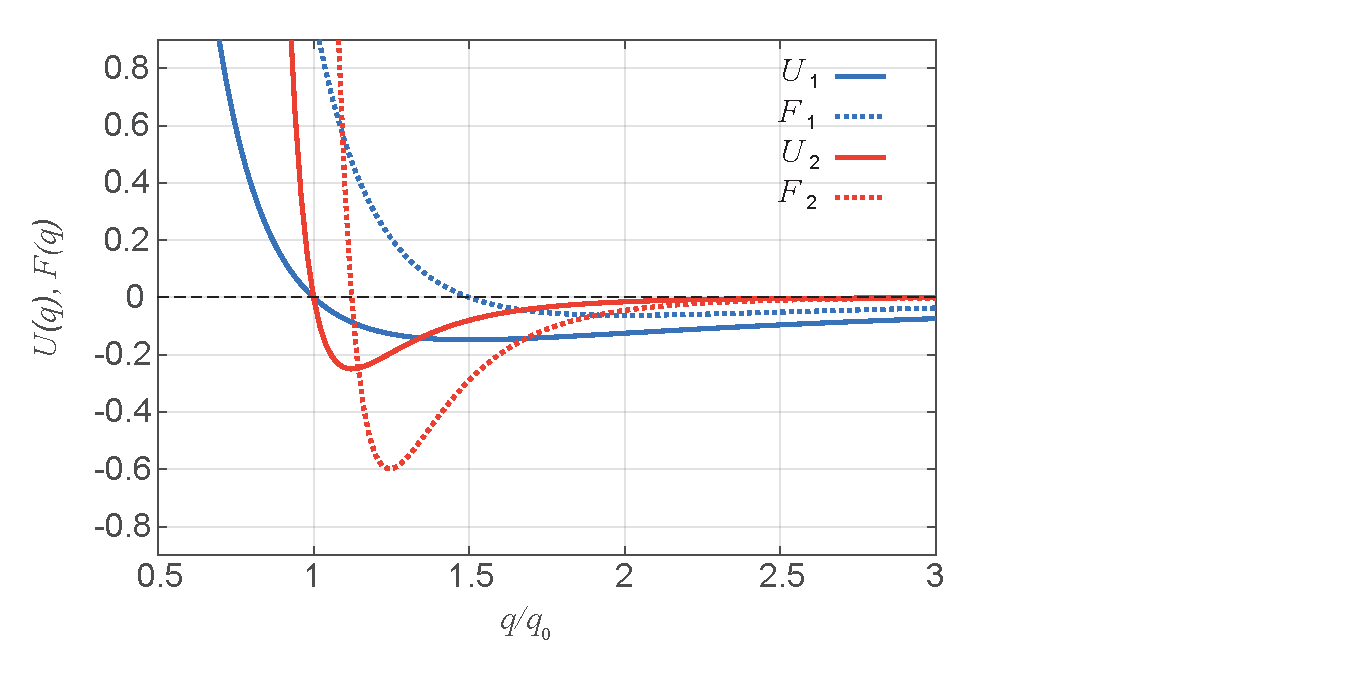
\includegraphics[width=\textwidth]{Molekuelpot01.pdf}
\caption[Potential und Kraftverlauf f�r zwei Molek�lpotentiale]{Potential- und Kraftverlauf f�r das Lennard-Jones-Potential (Index 1), sowie das Potential f�r heterogene zweiatomige Molek�le (Index 2)} 
\label{abb:bew_MolekuelPot01}
\end{figure}

\begin{figure}[H]\centering
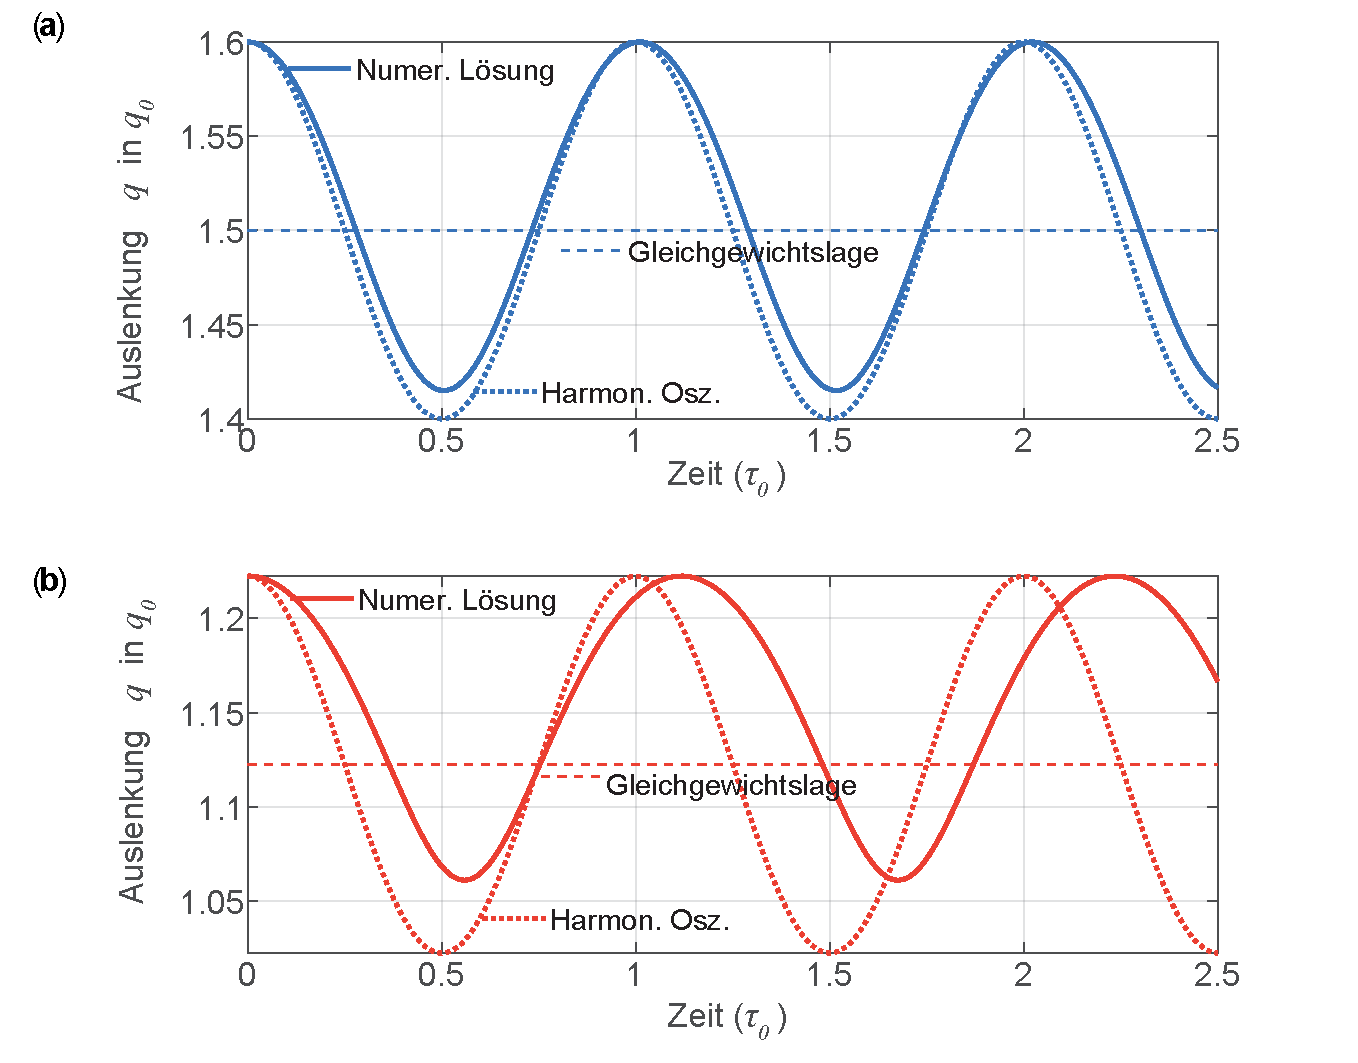
\includegraphics[width=\textwidth]{Molekuelpot02.pdf}
\caption[Schwingungsverl�ufe bei zweiatomigen Molek�len]{Schwingungsverl�ufe bei zweiatomigen Molek�len f�r das Lennard-Jones-Potential \fa und das Potential f�r ein heterogenes zweiatomiges Molek�l \fb} 
\label{abb:bew_MolekuelPot02}
\end{figure}

	\subprob{Modell f�r Nicht-Edelgas-Atome}
	H�ufig schreibt man das Potential f�r ein zweiatomiges Molek�l, das aus zwei unterschiedlichen Atomen besteht, wie folgt \cite{Timberlake2008}:
	\begin{equation}
		U(q) = \lk \frac{A}{q^3} - \frac{B}{q^2} \rk = \lk \tilde{\epsilon}_\text{A} \frac{{q_0}^3}{q^3} - \tilde{\epsilon}_\text{B} \frac{{q_0}^2}{q^2} \rk \label{eq:bew_Uebung22_04}~.
	\end{equation}
	Wir f�hren die Rechnungen analog zum ersten Aufgabenteil durch und erhalten folgende Ergebnisse:
	\begin{enumerate}[a)]
		\item Bindungsl�nge\\
			\begin{align*}
			&\frac{\partial U}{\partial q} \bigg|_{q_\text{B}} = -\frac{3A}{{q_\text{B}}^4}+ \frac{2B}{{q_\text{B}}^3} \overset{!}{=} 0  \\
			&\rightarrow q_\text{B} = \frac{3A}{2B}= \frac{3 \tilde{\epsilon}_\text{A}}{2 \tilde{\epsilon}_\text{B}} \, q_0 ~.
			\end{align*}
%\newpage
		\item Schwingungsfrequenz\\
			\begin{align}
				k_\text{eff} &= \frac{\partial^2}{\partial q^2}U(q) \bigg|_{q_\text{B}}
				= \frac{12A}{{q_\text{B}}^5}-\frac{6B}{{q_\text{B}}^4} \nonumber \\
				\rightarrow \omega^2 &= \frac{k_\text{eff}}{m_\text{eff}} = \frac{32B^5}{81 m_\text{eff}\,A^4} = \frac{32}{81} \frac{\tilde{\epsilon}_\text{B}{}^5}{\tilde{\epsilon}_\text{A}{}^4\,m_\text{eff} \, {q_0}^2}~. \label{eq:bew_Uebung22_05} 
			\end{align}
		\item Potential- und Anziehungskraftverlauf\\
			Als Vergleich zum Lennard-Jones-Potential von Aufgabenteil 1 sind in \figref{bew_MolekuelPot02} auch die Kurven f�r das Potential nach \eqref{eq:bew_Uebung22_04} berechnet und gezeigt.\\
	\end{enumerate} 

	\subprob{Zeitentwicklungen (Zusatz)}\\
		Beim Aufstellen der DGL f�r die \matlab-Routine \odevf{} haben wir folgende Vorgehensweise f�r die Zeiteichung gew�hlt.
		Die Schwingungsfrequenz ist in der harmonischen N�herung gegeben durch:
		\[ \omega_0^2 = \frac{k_\text{eff}}{m_\text{eff}} = \frac{1}{m_\text{eff}} \frac{\partial ^2}{\partial q^2}(-U) \bigg|_{q_\text{B}} ~,
		\]
		wobei $m_\text{eff}$ die effektive \bzw reduzierte Masse ist.
		Wir betrachten nun die beiden diskutierten Potentiale im Vergleich und nehmen auch vereinfachend an, dass $\tilde{\epsilon}_\text{A} = \tilde{\epsilon}_\text{B}$ ist.\\
		\begin{enumerate}[a)]
		\item Lennard-Jones-Potential\\
		F�r
		\[ U(q) = \frac{A}{q^{12}} - \frac{B}{q^6}
		\]
		mit $A= 4 \tilde{\epsilon}\,{q_0}^{12}$, $B= 4 \tilde{\epsilon}\,{q_0}^6$ und $q_\text{B} = \sqrt[6]{2}\,q_0$ ergibt sich als Schwingungsfrequenz
\begin{align}
			\omega_0^2 = \frac{72 \tilde{\epsilon}}{{q_0}^2 \,\sqrt[3]{2}\,m_\text{eff}}  \label{eq:bew_Uebung22_Z1}
\end{align}
		und entsprechend f�r die Periodendauer
		\[{T_\text{P}}^2 = \frac{\pi^2}{18} {q_0}^2 \,\sqrt[3]{2} \,\frac{m_\text{eff}}{\tilde{\epsilon}}~. \]
		Die DGL ist damit
		\[ \frac{\d}{\d t}\dot{q} = - \frac{\partial}{\partial q}U(q) = \frac{4 \pi^2}{18} \sqrt[3]{2} \,\frac{m_\text{eff}}{\tilde{\epsilon}} \lk \frac{12}{q^3} - \frac{6}{q^7} \rk~.	\]
	\item Nicht-Edelgas-Atome\\
		F�r 
		\[ U(q) = \frac{A}{q^3} - \frac{B}{q^2}
		\]
		mit $A= \tilde{\epsilon}{q_0}^3$, $B= \tilde{\epsilon}{q_0}^2$ und $q_\text{B} = \frac{3}{2} q_0$ ist die Schwingungsfrequenz
		\[{\omega_0}^2 = \frac{32}{81} \frac{\tilde{\epsilon}}{m_\text{eff}\,{q_0}^2} \]
		und die Periodendauer
		\[{T_\text{P}}^2 = \frac{81}{8} \pi^2 \,\frac{m_\text{eff}\,{q_0}^2}{\tilde{\epsilon}}~. \]
		Damit k�nnen wir die DGL schreiben als
		\[ \frac{\d}{\d t}\dot{q} = -\frac{\partial}{\partial q}U(q) = \frac{81}{8} \frac{m_\text{eff}}{\tilde{\epsilon}} \pi^2 \lk \frac{3}{q^4} - \frac{2}{q^3} \rk~.
		\]
	\end{enumerate}
		Wir erkennen, dass die gr��ere Anharmonizit�t beim Lennard-Jones-Potential auch schon bei kleinen Auslenkungen zu deutlichen Abweichungen vom Schwingungsverhalten des harmonischen Oszillators f�hrt.
		Deutlich erkennbar ist auch die gr��ere Asymmetrie in den Umkehrpunkten bedingt durch die nichtlinearen Terme in Form der h�heren Potenzen.
		Es ist sehr instruktiv, den Anfangswert $q_i$ im Programm zu ver�ndern und das Einsetzen der Anharmonizit�t zu beobachten. \\

	\subprob{Quantitative Absch�tzung (Zusatz)}
	Wir k�nnen die L�sung benutzen, um eine Absch�tzung f�r molekulare Schwingungsfrequenzen und Dissoziationsenergien nach einer klassischen Betrachtung zu erhalten.
        Wir wollen dies f�r ein Molek�l tun, das aus zwei Helium-Atomen besteht.
        F�r dieses System kann man die Parameter f�r das Lennard-Jones-Potential wie folgt annehmen:
\begin{align*}
\tilde{\epsilon}_\text{A} &= \tilde{\epsilon}_\text{B} =\SI{2.5e-22}{\J} = \tilde{\epsilon}
\qquad \text{und} \qquad q_0 =\SI{2.5e-10}{\metre}\,.
\end{align*}
	Die Tiefe des Potentialtopfes an der Stelle $q_\text{B}=\sqrt[6]{2}\,q_0$ ist aus \eqref{eq:bew_Uebung22_00} gegeben durch:
	\[
	E_\text{min} = -2 \tilde{\epsilon} = -\SI{5e-22}{\J}\,.
	\]
	In der Molekularphysik ist es �blich, Energien mittels Temperaturen eines Gleichgewichtssystems �ber 
\begin{align}
	E = k_\text{B} T \,\label{eq:bew_Uebung22_06}
\end{align}
auszudr�cken, worin $k_\text{B}= \SI{1.38064852e-23}{\J\per\K}$ die Boltzmann\footnote{Ludwig Eduard Boltzmann\indexp{Boltzmann, Ludwig Eduard} (1844--1906) war ein bedeutender �sterreichischer Physiker und arbeitete vor allem auf den Gebieten der Thermodynamik und der statistischen Mechanik.}-Konstante und $T$ die Temperatur in $\SI{}{\K}$ ist.
Demnach entspricht die Tiefe des Potentialtopfes gerade einmal einer Temperatur von $ T \approx \SI{18}{\K}$.
Da das Lennard-Jones-Potential auf seinem Definitionsbereich nur dieses eine Minimum besitzt und f�r $R \rightarrow\infty$ gegen Null geht, handelt es sich hierbei wirklich um die \anf{tiefste} Stelle des Potentials und nach der klassischen Mechanik w�re das auch die Bindungsenergie.
In der Quantenmechanik hat ein System nicht die minimale Energie eines Potentials, sondern besitzt immer mindestens eine sogenannte Nullpunktsenergie \cite{Schmutzer2005, Bartelmann2015}.
Diese Nullpunktsenergie kann man anschaulich als etwa die minimale relative Schwingung beider Heliumatome ansehen, die durch das Lennard-Jones-Potential erlaubt wird.
Die Frequenz dieser Schwingung hatten wir in \eqref{eq:bew_Uebung22_Z1} hergeleitet, woraus sich ergibt:
	\[\omega_0 = \SI{8.29e12}{\per\s} \quad \text{\bzw} \quad T_\text{P} = \SI{7.58e-13}{\s}\,.
\]
Die Energie einer solchen Schwingung ist nach der Quantentheorie durch $\frac{1}{2} \hbar\omega_0$ gegeben und berechnet sich damit zu:
	\[E_0 = \SI{4.37e-22}{\J} \quad \text{\bzw} \quad  T_0 = \SI{31.7}{\K}\,.
\]
Dieser Wert liegt signifikant oberhalb der maximalen Tiefe von 18\,K des Lennard-Jones-Potentials, sodass mit den angenommenen Werten f�r $q_0$ und $\tilde{\epsilon}$ keine stabilen
Heliummolek�le zu erwarten sind (zumindest nicht im Grundzustand), vielmehr werden diese, so sie sich irgendwie transient gebildet haben, sofort (d.h. ungef�hr in der Zeit $T_\text{P}$) dissoziieren.\footnote{In Experimenten mit ultrakaltem Helium \cite{Grisenti2000} hat man die Bindungsenergie $E_\text{B} = E_\text{min} + E_0$ zu ca. $\SI{1.1e-03}{\K}$ und den Bindungsradius zu $\SI{5.2e-09}{\metre}$ bestimmt, was ein extrem schwach gebundenes Molek�l darstellt.
Wir haben also in unserem einfachen Modell den Atomabstand massiv untersch�tzt.}
\end{subprobs}
\end{sol} 
%\href{PhysikUncut_Part1.pdf#prb:bew_Molekuelpotentiale}{\textcolor{blue} {$\rightarrow$ zur \probref{bew_Molekuelpotentiale}.}}\\
\textcolor{blue} {$\rightarrow$ zur} \probref{bew_Molekuelpotentiale}.\\
\noindent\rule[1ex]{\textwidth}{0.5pt}  \newpage

%-----------------------------------------------------------------------------------------------------------

\hypertarget{lsg:bew_Kopplung01}{}
\begin{sol}{prob:bew_Kopplung01}\label{lsg:bew_Kopplung01}%�bung28
\textbf{Zwei gekoppelte Stangenpendel.} \\ \\
Wir benutzen die Geometrie aus \figref{bew_Kopplg01}.
Wir kommen auf folgende Bewegungsgleichungen:
\begin{align}
		\ddot{\theta}_1 + {\omega_{\uproman{1}}}^2\sin\theta_1 + \kappa_{\uproman{1}}\, \lk \sin\theta_1-\sin\theta_2\rk \,\cos\theta1  &= 0 \,,\nonumber \\
		\ddot{\theta}_2 + {\omega_{\uproman{2}}}^2\sin\theta_2 - \kappa_{\uproman{2}}\, \lk \sin\theta_1-\sin\theta_2\rk \,\cos\theta2  &= 0 \,. \label{eq:bew_LsgKopplung01a}
\end{align}
Mit den N�herungen f�r kleine Winkel gilt:
\begin{align}
		\ddot{\theta}_1 + {\omega_{\uproman{1}}}^2\theta_1 + \kappa_{\uproman{1}}\, \lk \theta_1-\theta_2\rk &= 0 \,,\nonumber \\
		\ddot{\theta}_2 + {\omega_{\uproman{2}}}^2\theta_2 - \kappa_{\uproman{2}}\, \lk \theta_1-\theta_2\rk &= 0 \,. \label{eq:bew_LsgKopplung01}
\end{align}
Hier haben wir die Eigenfrequenzen 
\begin{equation*}
	\omega_\text{I}^2 = \frac{g}{l_{1}} 
	\qquad \text{und} \qquad 
	\omega_\text{II}^2 = \frac{g}{l_{2}}
\end{equation*}
sowie die effektiven Kopplungskonstanten
\begin{equation*}
	\kappa_{\uproman{1}} = \frac{\kappa\,{l_\text{F}}^2}{m_{1}\,{l_{1}}^2} \,\\
	\qquad \text{und} \qquad 
	\kappa_{\uproman{2}} = \frac{\kappa\,{l_\text{F}}^2}{m_{2}\,{l_{2}}^2}
\end{equation*}
verwendet. 
Die L�sung der charakteristischen Gleichung \eqref{eq:bew_Kopplg08} f�hrt f�r $\lambda_{1/2} = {\omega_{1/2}}^2$ auf die folgende Schwingungsfrequenzen:
\begin{align}
		{\omega_{1/2}}^2 &= \frac{{\omega_{\uproman{1}}}^2 + {\omega_{\uproman{2}}}^2 + \kappa_1 + \kappa_2}{2}\nonumber \\
		&\quad \pm \frac{1}{2} \sqrt{\lk {\omega_{\uproman{1}}}^2-{\omega_{\uproman{2}}}^2\rk^2 + \lk \kappa_1+\kappa_2 \rk^2+ 2\lk {\omega_{\uproman{1}}}^2 -{\omega_{\uproman{2}}}^2\rk \lk \kappa_1-\kappa_2\rk}\,.\label{eq:bew_LsgKopplung02}
\end{align}
Man beachte, dass hierin $\omega_1$ und $\omega_2$ die Normalfrequenzen des gekoppelten Systems darstellen, hingegen $\omega_{\uproman{1}}$ und $\omega_{\uproman{2}}$ die Eigenfrequenzen der einzelnen Pendel.
Wir widmen uns nun den konkreten Teilaufgaben mit den Angaben f�r die Pendell�ngen.
\begin{subprobs}
	\subprob{Pendel mit gleicher L�nge und Masse, kleine Winkel}
	Hier gilt $l_1 = l_2$ und $m_1 = m_2$.
	Au�erdem verwenden wir die Anfangsbedingungen 
	$\theta_1\lk 0\rk = \theta_0$, 
	$\theta_2\lk 0\rk = 0$, sowie
	$\dot{\theta}_{10}= 0$ und $\dot{\theta}_{20}= 0$.
	Dann erhalten wir mit $\kappa_1=\kappa_2=\kappa$ und $\omega_{\uproman{1}} = \omega_{\uproman{2}} = \omega_0$ als Frequenzen der Eigenschwingungen der beiden Pendel 
	\begin{align*}
			\omega_1  &= \omega_0 \,, \\
			\omega_2 &= \sqrt{{\omega_0}^2 + 2\kappa}\,.
	\end{align*}
	Die Normalschwingungen sind durch $\begin{pmatrix} 1 \\ 1 \end{pmatrix}$ \bzw $\begin{pmatrix} -1 \\ 1 \end{pmatrix}$ gegeben. 
	Wir wollen nun den Fall betrachten, dass ein Pendel zur Startzeit eine Auslenkung $\theta_{10}$ hat, wohingegen alle anderen Anfangsbedingungen Null sind. 
	Dann ergibt sich mit $C = \frac{\theta_0}{2}$ 
	\begin{align*}
			\theta_1 &= C\lk \cos\omega_1t + \cos\omega_2t\rk \,, \\
			\theta_2 &= C\lk \cos\omega_1t - \cos\omega_2t\rk\,.
	\end{align*}
	Man erkennt, dass die Auslenkungen $\theta_1$ , $\theta_1$ wegen der gleichen Kopplungskonstante, also wegen $\kappa_1 = \kappa_2$, reine Schwebungen darstellen.

\begin{figure}[H]\centering
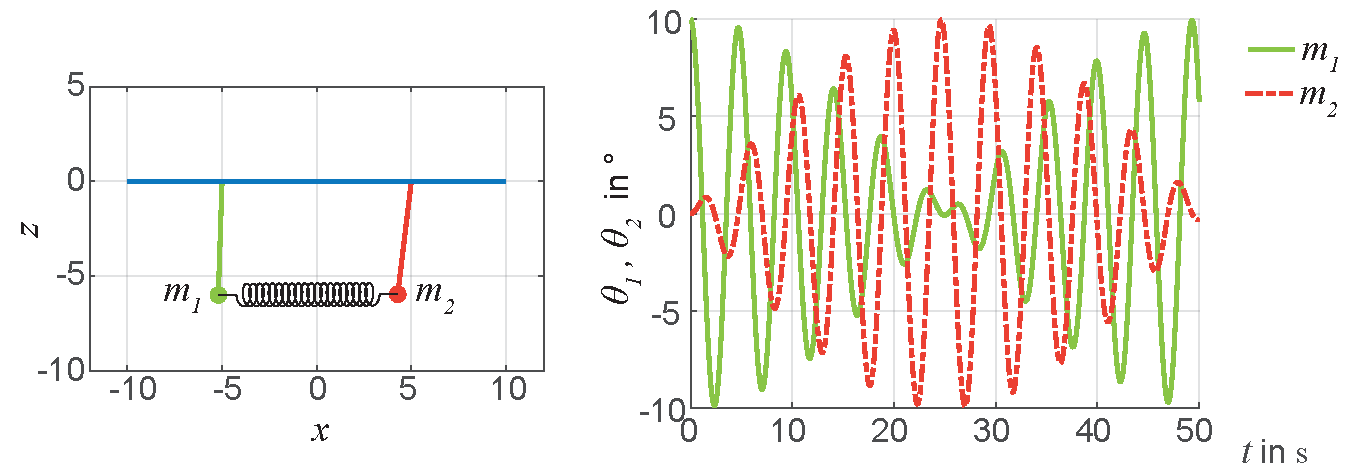
\includegraphics[width=\textwidth]{LsgGekopPendel01.pdf}%
\caption[Kleinwinkel-Schwingungsverhalten zweier gekoppelter Stangenpendel]{Kleinwinkel-Schwingungsverhalten zweier miteinander gekoppelter Stangenpendel gleicher L�nge und Masse. Deutlich ist das Schwebungsverhalten zu erkennen, \vgl \mlbewref{GekoppeltePendel01.m}. Parameter: $l_1 = l_2= \SI{6}{\metre}, m_1 = m_2 = \SI{3}{\kg}, D = \SI{0.5}{\N\per\metre}, \theta_{10} = 10\degree, \theta_{20} = 0\degree$ und $l_F = \SI{6}{\metre}$}
\label{abb:bew_LsgKopplung01}
\end{figure}

	\subprob{Pendel mit ungleicher L�nge, kleine Winkel}
	Hier gilt nun 
	$l_1 \neq l_2 \neq l_\text{F}$ und $m_1 \neq m_2$.
        Als Anfangsbedingungen verwenden wir die gleichen wie oben.
	Durch analoges Vorgehen erhalten wir
	\begin{align}
		{\omega_{1/2}}^2 &= \frac{{\omega_{\uproman{1}}}^2 + {\omega_{\uproman{2}}}^2 + \kappa_1 + \kappa_2}{2}\nonumber \\
		&\quad \pm\frac{1}{2}\lk {\omega_{\uproman{1}}}^2 - {\omega_{\uproman{2}}}^2\rk\sqrt{1+2\frac{\kappa_1-\kappa_2}{{\omega_{\uproman{1}}}^2-{\omega_{\uproman{2}}}^2}+\lk \frac{\kappa_1+\kappa_2}{{\omega_{\uproman{1}}}^2-{\omega_{\uproman{2}}}^2}\rk^2   }\,.
		\label{eq:bew_LsgKopplung03}
	\end{align}
	F�r kleinere Kopplungsst�rken, d.h. f�r $\kappa_1 \pm \kappa_2 \ll {\omega_{\uproman{1}}}^2-{\omega_{\uproman{2}}}^2$ kann man die Wurzel als Reihe entwickeln. (Das geht offensichtlich nicht, wenn ${\omega_{\uproman{1}}}^2 \approx {\omega_{\uproman{2}}}^2$, aber eben diesen Fall haben wir ja in Teilaufgabe 1 behandelt).
	Wir erhalten als Normalfrequenzen
	\begin{align*}
		{\omega_1}^2 &= {\omega_{\uproman{1}}}^2 + \kappa_1 + \frac{\kappa_1\kappa_2}{{\omega_{\uproman{1}}}^2-{\omega_{\uproman{2}}}^2} \,, \\
		{\omega_2}^2 &= {\omega_{\uproman{2}}}^2 + \kappa_2 -\frac{\kappa_1\kappa_2}{{\omega_{\uproman{1}}}^2-{\omega_{\uproman{2}}}^2} \,.
	\end{align*}
	und k�nnen damit auch die entsprechenden Schwingungen analytisch berechnen. 
	F�r die vorgegebenen Randbedingungen erhalten wir:
	\begin{align*}
		\theta_1 &= \frac{\theta_{10}}{C_1-C_2} \lk C_1\cos\omega_1 t - C_2\cos\omega_2 t\rk \,, \\
		\theta_2 &= \frac{\theta_{10}}{C_1-C_2} \lk \cos\omega_1 t - \cos\omega_2 t\rk \,, \\
	\end{align*}
	worin 
		\[C_1 = \frac{\omega_{\uproman{2}}^2-{\omega_1}^2 + \kappa_2}{\kappa_2}~~\text{und}~~C_2 = \frac{\omega_{\uproman{2}}^2-{\omega_2}^2 + \kappa_2}{\kappa_2}
	\]
	sind.
        Man erkennt, dass $\theta_1$ auch hier keine reine Schwebung mehr darstellt.
	Es ist also schon jetzt sehr vorteilhaft, das Problem numerisch anzugehen.
        Wir haben dies in \mlbewref{GekoppeltePendel02.m} getan.

\begin{figure}[H]\centering
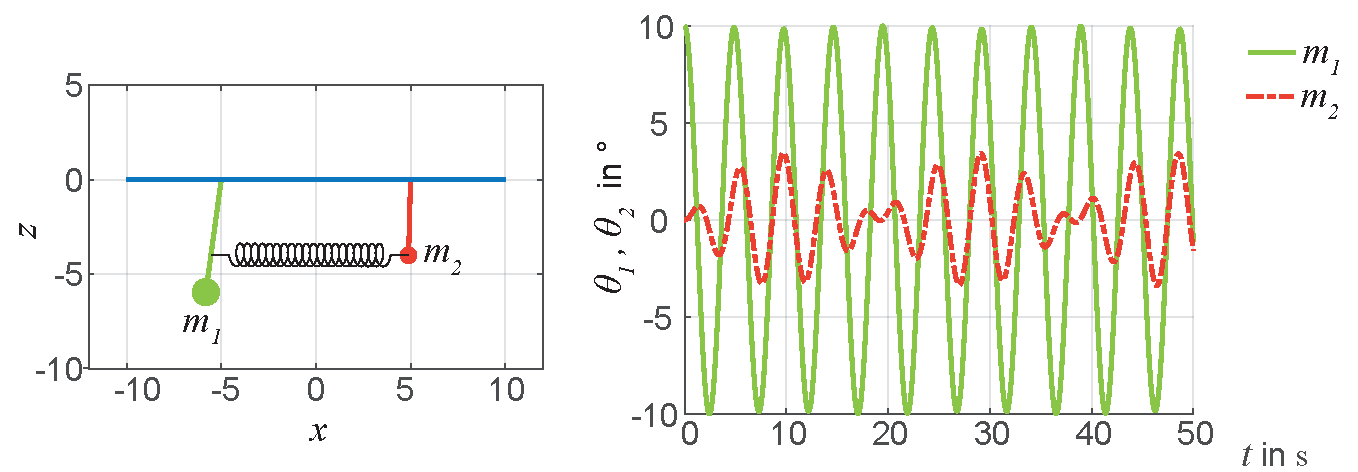
\includegraphics[width=\textwidth]{LsgGekopPendel02.pdf}%
\caption[Kleinwinkel-Schwingungsverhalten zweier gekoppelter Stangenpendel]{Kleinwinkel-Schwingungsverhalten zweier miteinander gekoppelter Stangenpendel unterschiedlicher L�nge. Deutlich ist das Schwebungsverhalten f�r $\theta_2$ zu erkennen, w�hrend $\theta_1$ keine Schwebung mehr darstellt. Parameter: $l_1 = \SI{6}{\metre}, 
l_2 = \SI{4}{\metre}, m_1 = \SI{5}{\kg}, m_2 = \SI{3}{\kg}, D2 = \SI{0.5}{\N\per\metre}, \theta_{10} = 10\degree, \theta_{20} = 0\degree$ und $l_F = \SI{4}{\metre}$}
\label{abb:bew_LsgKopplung02}
\end{figure}

	\subprob{Beliebig gro�e Auslenkungen und unterschiedlich lange Pendel}
	Die L�sung ist in \mlbewref{GekoppeltePendel03.m} ausgef�hrt.\\
		
\begin{figure}[H]\centering
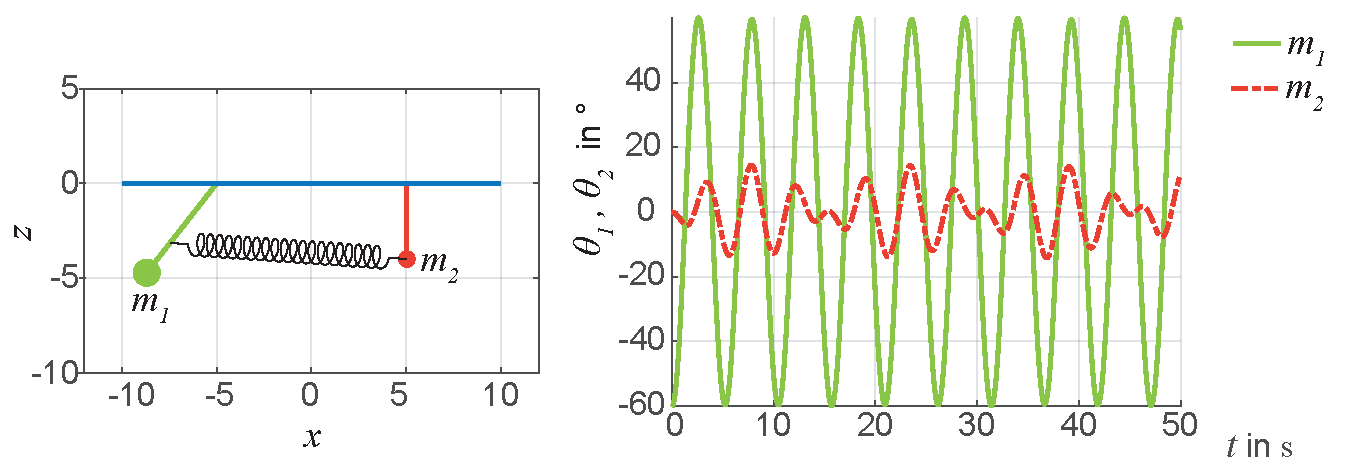
\includegraphics[width=\textwidth]{LsgGekopPendel03.pdf}%
\caption[Schwingungsverhalten zweier gekoppelter Stangenpendel]{Schwingungsverhalten zweier miteinander gekoppelter Stangenpendel. Parameter: $l_1 = \SI{6}{\metre}, l_2 = \SI{4}{\metre}, m_1 = \SI{5}{\kg}, m_2 = \SI{3}{\kg}, D2 = \SI{0.5}{\N\per\metre}, \theta_{10} = 60\degree, \theta_{20} = 0\degree$ und $l_F = \SI{4}{\metre}$}
\label{abb:bew_LsgKopplung03}
\end{figure}

\end{subprobs}

\end{sol} 
%\href{PhysikUncut_Part1.pdf#prb:bew_Kopplung01}{\textcolor{blue} {$\rightarrow$ zur \probref{bew_Kopplung01}.}}\\
\textcolor{blue} {$\rightarrow$ zur} \probref{bew_Kopplung01}.\\
\noindent\rule[1ex]{\textwidth}{0.5pt}  \newpage


%-----------------------------------------------------------------------------------------------------------

\hypertarget{lsg:bew_CO2Molekuel}{}
\begin{sol}{prob:bew_CO2Molekuel}\label{lsg:bew_CO2Molekuel} %%�bung29
\textbf{Schwingungen des  $\text{CO}_2$-Molek�ls} \\
\begin{subprobs}
\subprob{Streckschwingungen des Molek�ls}
In der \probref{bew_Molekuelpotentiale} Molek�lpotentiale hatten wir Approximationen der tats�chlichen Kr�fte zwischen den Atomen gefunden, die zu einem nichtlinearen Verhalten f�hrten. 
Wir werden am Ende dieser �bung noch auf diese eingehen, wollen uns aber zun�chst auf den einfachen Fall der harmonischen N�herung beschr�nken. Wir modellieren das CO$_2$-Molek�l zun�chst als \emph{linearen} Federschwinger, beschreiben die Kraft also in der N�herung $\keff\, x$. 
Als Lagrange-Funktion ergibt sich damit 
\begin{align}
    \mathcal{L} &= T -U \nonumber \\
    &= \frac{m_\text{O}^2}{2}\lk \dot{x_1}^2  + \dot{x_3}^2 \rk + \frac{m_\text{C}}{2}\dot{x_2}^2 - \frac{\keff}{2} \lk (x_2 - x_1 - L)^2 + (x_3 - x_2 - L)^2\rk
    \label{eq:bew_CO2M01}~.
\end{align}
Wir setzen  $q_1 = x_1 - L$, $q_2 = x_2$ und $q_3 = x_3 - L$.
Mit diesen generalisierten Koordinaten 
\begin{equation}
    \vec{q} = 
    \begin{pmatrix}
    	q_1 \\ q_2 \\ q_3
    \end{pmatrix}
    \label{eq:bew_CO2M02}
\end{equation}
k�nnen wir $T$ und $U$ mit den Matrizen $\mathbb{T}$ und $\mathbb{U}$ folgenderma�en schreiben:
\begin{align}
    T &= \frac{1}{2} \dot{\vec{q}}^T \mathbb{T} \dot{\vec{q}}
    \qquad &\text{mit} \qquad
    \mathbb{T} &= 
    \begin{pmatrix}
        m_\text{O} & 0 & 0 \\
        0 & m_\text{C} & 0 \\
        0 & 0 & m_\text{O}
    \end{pmatrix} \nonumber \\
    U &= \frac{\keff}{2} \sum_{i,j = 1}^3 q_i q_j U_{ij}
    \qquad &\text{mit} \qquad 
    \mathbb{U} &= \keff
    \begin{pmatrix}
        1 & -1 & 0 \\
        -1 & 2 & -1 \\
        0 & -1 & 1
    \end{pmatrix}~.
    \label{eq:bew_CO2M03}
   \end{align} 
   W�hrend die Matrix der kinetischen Energie $\mathbb{T}$ diagonalisiert ist, zeigen die Nebendiagonalelemente von $\mathbb{U}$, dass die Schwingungen gekoppelt sind.
   Die generalisierten Koordinaten $q_1$ und $q_3$ sind entkoppelt, f�r die urspr�nglichen Koordinaten $x_1$ und $x_3$ w�rde das nicht gelten.
   Wir bestimmen die Eigenwerte $\lambda$ aus der charakteristischen Gleichung \eqref{eq:bew_Kopplg08}: 
   \begin{equation}
       \det(\mathbb{U} - \lambda \mathbb{T}) = 
       \begin{vmatrix}
           \keff-\lambda\,m_\text{O} & -\keff & 0 \\
           -\keff & 2 \keff - \lambda\,m_\text{C} & - \keff \\
           0 & -\keff & \keff - \lambda\, m_\text{O}
       \end{vmatrix}
       = 0 
       \label{eq:bew_CO2M04}
   \end{equation}
   und erhalten die in $\lambda$ kubische Gleichung
   \begin{equation}
        (\keff - \lambda\, m_\text{O}) \lek (2 \keff - \lambda\, m_\text{C})(\keff -\,\lambda\, m_\text{O}) - {\keff}^2 \rek
        - {\keff}^2 \,(\keff - \lambda\,m_\text{O}) = 0~.
        \label{eq:bew_CO2M05}
    \end{equation} 
    Man findet damit
    \begin{align}
        \lambda_1 &= \frac{\keff}{m_\text{O}} = {\omega_{1,0}}^2 > 0 \nonumber \\
        \lambda_2 &= \lk \frac{\keff}{m_\text{O}} + \frac{2 \keff}{m_\text{C}} \rk = {\omega_{2,0}}^2 > 0 \nonumber \\
        \lambda_3 &= 0 \label{eq:bew_CO2M06}~.
    \end{align}
    Die Eigenwerte $\lambda_1$ und $\lambda_2$ sind verschieden von 0 und ergeben Schwingungsfrequenzen f�r Eigenschwingungen, w�hrend $\lambda_3 = 0$ bedeutet, dass hier eine reine Translation vorliegt.
    Wir bestimmen die beiden Eigenschwingungen nach \eqref{eq:bew_Kopplg07} zun�chst f�r $\lambda_1$:
    \begin{equation}
        (\mathbb{U} - \lambda_1 \mathbb{T}) \vec{n}_1 = 
        \begin{pmatrix}
            0 & -\keff & 0 \\
            -\keff ~~~& \keff \lk2-\frac{m_\text{C}}{m_\text{O}}\rk ~~~& -\keff \\
            0 & -\keff & 0
        \end{pmatrix}
        \begin{pmatrix}
            n_{1,1} \\ n_{1,2} \\ n_{1,3}
        \end{pmatrix}
        = 0~, \label{eq:bew_CO2M07}
    \end{equation}
    wobei wir der Einfachheit halber durch $m_\text{O}$ dividiert haben.
    Daraus folgt $n_{1,2} = 0$  und $n_{1,3} = -n_{1,1}$, \bzw
    \begin{equation}
        \vec{n}_1 = C
        \begin{pmatrix}
            1 \\ 0 \\ -1
        \end{pmatrix}
        \label{eq:bew_CO2M08}~.
    \end{equation}
    Den Vorfaktor bestimmen wir aus der Forderung nach Normierung der Eigenschwingung
		\[	{\vec{n}_i}^T ~ \mathbb{T} ~ \vec{n}_j = \delta_{ij}
\] 	 zu $C = \frac{1}{\sqrt{2m_\text{O}}}$. 
    Analog erh�lt man f�r den zweiten Eigenwert  $\lambda_2$ den Eigenvektor:
    \begin{equation}
        \vec{n}_2 = \sqrt{\frac{m_\text{C}}{2m_\text{O} (2m_\text{O}+m_\text{C})}} 
        \begin{pmatrix}
            1 \\ -2m_\text{O}/m_\text{C} \\1
        \end{pmatrix} \,.
        \label{eq:bew_CO2M09}
    \end{equation}
    F�r den dritten Eigenwert finden wir:
    \begin{equation}
        \vec{n}_3 = \sqrt{\frac{1}{2m_\text{O} +m_\text{C}}} 
        \begin{pmatrix}
            1 \\ 1 \\1
        \end{pmatrix}
        \label{eq:bew_CO2M10}~.
    \end{equation}
    Zur Berechnung kann man die \matlab{} Symbolic Toolbox verwenden.
    Interessant ist, dass die Eigenfrequenzen von $\keff$, $m_\text{O}$ und $m_\text{C}$ abh�ngen, die Eigenvektoren hingegen nur von den Massen.
    Wie man an \eqref{eq:bew_CO2M08} erkennt, entspricht die Eigenschwingung $\vec{n}_1$ einer antisymmetrischen (!) Schwingung der Sauerstoff-Atome.
    Das Kohlenstoff-Atom bleibt allerdings in Ruhe. Dies wird symmetrische (!) Streckschwingung (\figref{bew_CO2Molekuel02}\,a) genannt.\footnote{Gezielte Verwirrung ist manchmal Teil des Physik-Curriculums.}
    Bei $\vec{n}_2$ schwingen die Sauerstoff-Atome gleichphasig, aber das Kohlenstoff-Atom gegenphasig zu diesen. Man spricht hier von einer antisymmetrischen (!) Streckschwingung (\figref{bew_CO2Molekuel02}\,b).
    Der Eigenvektor $\vec{n}_3$ beschreibt eine Bewegung des Gesamtsystems entlang der $x$-Achse (Translation) und bedeutet gerade die Gesamtimpulserhaltung.
    Damit ist die Gesamtbewegung
    \begin{equation}
        \vec{q}(t) = 
        \begin{pmatrix}
            q_1(t) \\ q_2(t) \\ q_3(t)
        \end{pmatrix}
        =
        \begin{pmatrix}
        \vec{n}_1 A_1 \cos(\omega_{1,0}t -\delta_1) \\
        \vec{n}_2 A_2 \cos(\omega_{2,0}t -\delta_2) \\
        \vec{n}_3 (q_{3,0} + \dot{q}_{3,0})
        \end{pmatrix},
        \label{eq:bew_CO2M11}
    \end{equation}
    wobei sich die Konstanten $A_1$, $A_2$, $\delta_1$ und $\delta_2$ aus den Anfangsbedingungen ergeben, genauso wie die $q_{3,0} = q_3(t=0)$ und $\dot{q}_{3,0} = \dot{q}_3(t=0)$.
    In kartesischen Koordinaten erh�lt man durch R�cksubstitution
    \begin{equation}
        \vec{x}(t) = 
        \begin{pmatrix}
            x_1(t) \\ x_2(t) \\ x_3(t)
        \end{pmatrix}
        =
        \begin{pmatrix}
            q_1(t) - L \\ q_2(t) \\ q_3(t)+L
        \end{pmatrix}
        \label{eq:bew_CO2M12}.
    \end{equation}
    Wir wollen nun noch kurz betrachten, wie die Schwingen f�r realistischere Molek�l\-potentiale aussehen.
    Wir hatten diese schon in \probref{bew_Molekuelpotentiale}
    berechnet und in der linearen N�herung f�r die Federkonstante folgendes erhalten:
    \begin{equation}
        \keff = \frac{\partial^2}{\partial q^2} U(q) \big|_{q_B} 
        = \frac{32}{81} \frac{\varepsilon}{{q_0}^2}.
    \end{equation}
    Darin waren $\varepsilon$ und $q_0$ molekulare Parameter. 
    Wir kommen damit in der harmonischen N�herung nat�rlich wieder auf die Eigenschwingungen \eqref{eq:bew_CO2M11}, im anharmonischen Fall mit den Molek�l\-potentialen k�nnen wir das System nur noch numerisch l�sen.
    %Die Ergebnisse sind f�r zwei verschiedene Anfangsbedingungen in \figref{bew_CO2Molekuel03} gezeigt.
    %Man erkennt, dass bei kleinen Auslenkungen die Eigenschwingungen erhalten bleiben (wie zu erwarten war) und das Ergebnis gut mit der harmonischen N�herung \eqref{eq:bew_CO2M11} �bereinstimmt. 
    %Bei gr��eren Auslenkungen entstehen zus�tzlichen Frequenzen (ebenfalls erwartet!), wie man sch�n am Frequenzspektrum sieht.\\
\subprob{Deformationsschwingungen des Molek�ls}
	Wir wollen jetzt noch die sogenannte Deformations- und Knickschwingung des Molek�ls modellieren.
        Dies sind Schwingungen senkrecht zur Hauptachse des Molek�ls.
    Da wir als Gleichgewichtslage das gestreckte Molek�l auf der $x$-Achse annehmen, k�nnen wir die Bewegungen in $x$- und $y$-Richtung vollst�ndig entkoppeln.
    F�r die $y$-Richtung ergeben sich die einfachen Energien
    \begin{align}
        T &= \frac{m_\text{O}}{2} \lk {\dot{y}_1}{}^2 + {\dot{y}_3}{}^2 \rk \nonumber \\
        U &= \frac{\keff}{2} \lek (y_2-y_1)^2 + (y_3-y_2)^2 \rek
        \label{eq:bew_CO2M13}~.
    \end{align}
    Sowohl die $\mathbb{T}$-, als auch die $\mathbb{U}$-Matrix sind dann identisch mit denen nach \eqref{eq:bew_CO2M03}, da wir hier einfach $q_i = y_i$ setzen k�nnen.
    Wir erhalten damit die gleichen Eigenvektoren und k�nnen sofort die L�sung aufschreiben:
    \begin{equation}
        \vec{y}(t) =
        \begin{pmatrix}
            y_1(t) \\ y_2(t) \\y_3(t)
        \end{pmatrix} =
        \begin{pmatrix}
            q_1(t) \\q_2(t) \\q_3(t)
        \end{pmatrix} =
    \begin{pmatrix}
        \vec{n}_1 A_1 \cos(\omega_{1,0}t - \delta_1) \\
        \vec{n}_2 A_2 \cos(\omega_{2,0}t - \delta_2) \\
        \vec{n}_3 (q_{3,0} + \dot{q}_{3,0})
    \end{pmatrix}.
    \end{equation}
    Die Interpretation ist allerdings hier eine andere: Die Normalschwingung $\vec{n}_1$ ist eine Art Rotation, die Normalschwingung $\vec{n}_2$ ist die sogenannte symmetrische Knickschwingung (\figref{bew_CO2Molekuel02}\,c) und $\vec{n}_3$ ist wiederum eine Translation, diesmal in $y$-Richtung. Wir wollen noch darauf hinweisen, dass man bei der Zuordnung unterschiedlicher Ladungsverteilungen auf die einzelnen Atome bei der antisymmetrischen Streckschwingung und bei der Knickschwingung eine �nderung des Dipolmoments des Molek�ls bekommt. Deswegen kann man diese Schwingungen im Infrarot-Bereich sehen.
\begin{figure}
\centering

\includegraphics[width=0.9\textwidth]{CO2Molekuel02.pdf}%
\caption[Schwingungsmoden eines dreiatomigen Molek�ls ($\text{CO}_2$-Molek�l)]{Schwingungsmoden eines dreiatomigen Molek�ls. \fa Symmetrische Streckschwingung \fb Antisymmetrische Streckschwingung \fc Knickschwingung}
\label{abb:bew_CO2Molekuel02}
\end{figure}
%
%\begin{figure}[H]\centering
%
\includegraphics[width=\textwidth]{Platzhalter.pdf}%
%\caption[Asymmetrische Streckschwingung eines dreiatomigen Molek�ls ($\text{CO}_2$-Molek�l) f�r verschiedene Auslenkungen und Frequenzspektrum.]{Simulation der asymmetrischen Streckschwingung eines dreiatomigen Molek�ls ($\text{CO}_2$-Molek�l) f�r verschiedene Auslenkungen und Frequenzspektrum.(\mlbewref{MolekschwingungCO2.m}.}
%\label{abb:bew_CO2Molekuel03}
%\end{figure}
%
\end{subprobs}
\end{sol} 
%\href{PhysikUncut_Part1.pdf#prb:bew_CO2Molekuel}{\textcolor{blue} {$\rightarrow$ zur \probref{bew_CO2Molekuel}.}}\\
\textcolor{blue} {$\rightarrow$ zur} \probref{bew_CO2Molekuel}.\\
\noindent\rule[1ex]{\textwidth}{0.5pt}  \newpage


%-----------------------------------------------------------------------------------------------------------
\hypertarget{lsg:bew_Stossdaempfer}{}
\begin{sol}{prob:bew_Stossdaempfer} \label{lsg:bew_Stossdaempfer} %�bung30
\textbf{Sto�d�mpfer, Schwingungstilgung f�r Tische und in Hochh�usern.} \\ \\
Wir k�nnten nat�rlich alle drei Teilaufgaben mit den in Kap.~\ref{kap:bew_Tilgung} gezeigten Methoden l�sen, dies sei auch dem Leser zur zus�tzlichen �bung empfohlen. Wir wollen hier aber auch jeweils auf das vorliegende Problem eine spezifische auch f�r die numerische Berechnung geeignete L�sungsmethode zeigen.
\begin{subprobs}
	\subprob{Sto�d�mpfer eines Autos}
	Die Aufgabe von Sto�d�mpfern ist es, die Schwingungen des gefederten Fahrzeugs (\zb beim Durchfahren eines Schlaglochs) entsprechend zu d�mpfen.
  Dabei soll insbesondere vermieden werden, dass es zu Schwingungen im Bereich der Eigenfrequenzen (und damit m�glicherweise zur sogenannten \anf{Resonanzkatastrophe}) kommt. 	Oft wird irrt�mlicherweise angenommen, dass der Sto�d�mpfer die Fahrbahnunebenheiten abf�ngt, das ist jedoch Aufgabe der Federung. Die Feder muss die dadurch gespeicherte Energie aber wieder abgeben. Das passiert �ber Schwingungen, die �ber die Kolbenstange auf den Sto�d�mpfer �bertragen werden. Die Bewegungsenergie wird dabei durch hydraulische Widerst�nde innerhalb des Sto�d�mpfers in W�rme umgewandelt. Das Funktionsprinzip des einfachen Einrohr-Sto�d�mpfers ist in \figref{bew_Stossdaempfer02} gezeigt.

\begin{figure}
\centering

\includegraphics[width= 0.9\textwidth]{Stossdaempfer02.pdf}%
\caption[Prinzip und Aufbau eines Stossd�mpfers]{ \fa Prinzip des Sto�d�mpfers \fb Aufbau eines Einrohr-Sto�d�mpfers 
(\href{https://www.tunero.de/service/funktion-sportdaempfer.html}{https://www.tunero.de/service/funktion-sportdaempfer.html}).
Schwingt das Fahrzeug nach unten zur Fahrbahn hin, wird der Arbeitskolben des Sto�d�mpfers nach unten gedr�ckt (Bild links).
Ein Ventil setzt dem �l, das aus der unteren Kammer nach oben str�mt (roter Pfeil), einen Widerstand entgegen und bremst somit die Abw�rtsbewegung.
Der Trennkolben wird dabei nach unten geschoben. 
Schwingt das Fahrzeug nach oben (Bild rechts), wird der Sto�d�mpfer durch die sich nach oben bewegende Kolbenstange wieder auseinandergezogen.
Ein zweites Ventil setzt dem �l wiederum einen hydraulischen Widerstand entgegen (gr�ner Pfeil), was die Aufw�rtsbewegung des Fahrzeugs d�mpft}
%Der Trennkolben geht nun wieder nach oben.}
\label{abb:bew_Stossdaempfer02}
\end{figure}

F�r die physikalische Modellierung nutzen wir das Modell nach \figref{bew_Stossdaempfer02}\,a. Danach ist $z_\text{A}$ der Federweg des Autos und $z_\text{D}$ der Federweg des D�mpfers mit der D�mpfungskonstanten $\eta_\text{D}$. Die Lagrange-Funktion lautet:
	\begin{align}
			\mathcal{L} = \frac{m_\text{A}}{2}{\dot{z}_\text{A}{}}^2 - \frac{k_\text{A}}{2}{z_\text{A}}^2 + \underbrace{\frac{m_\text{D}}{2}{\dot{z}_\text{D}{}}^2}_{\substack{=0}} + - \frac{k_\text{D}}{2} \lk z_\text{A} - z_\text{D} \rk^2 \,, \label{eq:bew_Stossdaempfer01}
	\end{align}
	woraus unter Ber�cksichtigung der Dissipationsfunktion die Bewegungsgleichungen 
	\begin{align}
	\begin{split}
			m_\text{A}\,\ddot{z}_\text{A} + k_\text{A}\,z_\text{A} + k_\text{D}\lk z_\text{A}-z_\text{D}\rk &= 0 \,,\\
			\eta_\text{D}\,\dot{z}_\text{D} - k_\text{D}\lk z_\text{A} -z_\text{D}\rk &= 0 \, \label{eq:bew_Stossdaempfer02}
	\end{split}
	\end{align}
	folgen. Hierbei haben wir die Masse des Sto�d�mpfers als sehr klein angenommen, also $m_\text{A} \gg m_\text{D} \approx 0$. \\
	Die charakteristische Gleichung \eqref{eq:bew_Kopplg08} f�hrt mit einem Ansatz f�r die Schwingungen von $z_\text{A,D} = C_\text{A,D}\,e^{\lambda\,t}$ auf folgende kubische Gleichung in $\lambda$ 
				\begin{align}
						\lambda^3 &= f\lk m_\text{A},k_\text{A},k_\text{D},\eta_\text{D}\rk \nonumber \\
						 \rightarrow 0 &= \lambda^3 + \frac{k_\text{D}}{\eta_\text{D}}\lambda^2 + \frac{k_\text{A}+k_\text{D}}{m_\text{A}}\lambda + \frac{k_\text{A}\,k_\text{D}}{m_\text{A} \eta_\text{D}} \,. \label{eq:bew_Stossdaempfer03}
				\end{align}
				
Aus dieser kann man die Eigenfrequenzen des Sto�d�mpfers berechnen oder umgekehrt bei Vorgabe dieser Frequenzen die Auslegung durch die Parameter $\eta_\text{D}$ \bzw $k_\text{D}$ bestimmen.
Wir wollen hier aber die Bewegungsgleichungen numerisch l�sen, um auch das Einschwingverhalten zu sehen. Das Ergebnis ist in \figref{bew_Stossdaempfer02}\,b zu sehen.

\begin{figure}[H]\centering
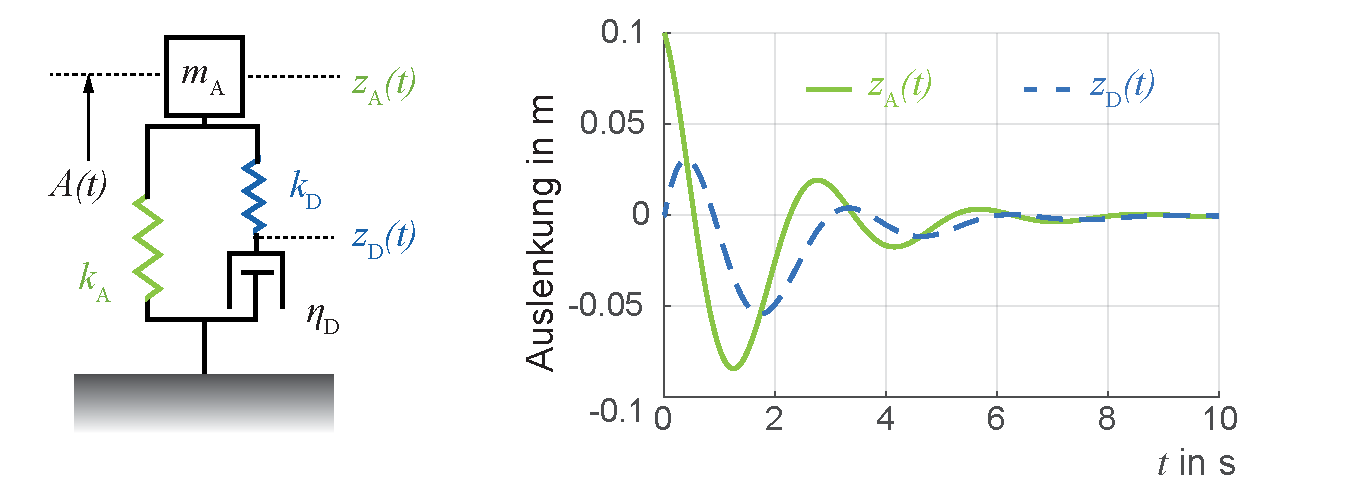
\includegraphics[width=\textwidth]{Stossdaempfer03.pdf}%
\caption[D�mpfung eines Fahrzeuges mit Sto�d�mpfer.]{D�mpfung eines Fahrzeuges mit Sto�d�mpfer f�r typische Parameter: Masse Auto $\SI{2000}{\kilo\gram}$, Federkonstante Auto $\SI{3000}{\N\per\metre}$,  Federkonstante Sto�d�mpfer $\SI{8000}{\N\per\metre}$, D�mpfung Sto�d�mpfer $\SI{5000}{\kg\per\s}$, \vgl \mlbewref{VibDaempfung01.m}} 
\label{abb:bew_Stossdaempfer03}
\end{figure}
			
\newpage
	\subprob{Schwingungstilgung bei Tischen und Deckenaufh�ngungen}

Wir berechnen den Fall der Schwingungsd�mpfung eines an einer Decke h�ngenden Ger�tes (\zb eines Operationsmikroskops)
der Masse $m_\text{G}$, die zur Tilgung angebrachte Gegenmasse sei $m_\text{T}$. Die Lagrange-Funktion lautet
\begin{align}
  \mathcal L=T-U
  &=\frac{m_\text{G}}{2}{\dot{z}_\text{G}}{}^2+\frac {m_\text{T}}{2}{\dot{z}_\text{T}}{}^2 - \frac{k_\text{G}}2\,{z_\text{G}}{}^2 - \frac{k_\text{T}}2\,(z_\text{T}-z_\text{G})^2 \,,
  \label{bew_tilgung01}
\end{align}

woraus sich die Lagrange-Gleichungen bei Ber�cksichtigung von D�mpfung $\eta_\text{G}, \eta_\text{T}$
und einer externen harmonischen Anregung 
\begin{align}
  m_\text{G}\,\ddot{z}_\text{G}+\eta_\text{G}\,\dot{z}_\text{G} + (k_\text{G}+k_\text{T})\,z_\text{G}-k_\text{T}\,z_\text{T} & = k_\text{G}\,A_\text{ext}\,\e^{i\omega t} \notag\\
  m_\text{T}\,\ddot{z}_\text{T}+\eta_\text{T}\,\dot{z}_\text{T} + k_\text{T}\,(z_\text{T}-z_\text{G})        & = 0
  \label{bew_tilgung02}
\end{align}
ergeben. F�r die spezielle inhomogene L�sung\footnote{Wegen der D�mpfung ist nur die spezielle L�sung der inhomogenen
Differentialgleichung\index{Differentialgleichung!inhomogene} relevant.} machen wir den Ansatz
\begin{align}
  z_\text{G} = A_\text{G}\,\e^{\im(\omega t-\varphi_\text{G})}\,,~~~z_\text{T} = A_\text{T}\, \e^{\im(\omega t-\varphi_\text{T})}\,,
  \label{bew_tilgung03}
\end{align}
was auf
\begin{align}
\begin{split}
  A_\text{G}\left[-m_\text{G}\omega^2+\im\,\eta_\text{G}\omega+k_\text{G}+k_\text{T}\right]e^{-i\varphi_\text{G}}
  -A_\text{T}[k_\text{T}]\,\e^{-\im\varphi_\text{T}}
  &=k_\text{G} A_\text{ext} \\
  A_\text{G}[-k_\text{T}]\e^{-\im\varphi_\text{G}}+A_\text{T}\left[-m_\text{T}\omega^2+\im\,\eta_\text{T}\omega+k_\text{T}\right]e^{-\im\varphi_\text{T}}&=0
\end{split}   \label{bew_tilgung04}
\end{align}
f�hrt.
Das ist ein lineares Gleichungssystem in $A_\text{G}$ und $A_\text{T}$. In der zweiten Gleichung von \eqref{bew_tilgung04} sind $A_\text{G}$ und $A_\text{T}$ reell, deshalb gilt:
\begin{align}
\begin{split}
  A_\text{T} = \frac{k_\text{T}}{\sqrt{(k_\text{T}-m_\text{T}\,\omega^2)^2+(\eta_\text{T}\,\Omega)^2}}A_\text{G} ~~~\text{und}\\
	\sqrt{(k_\text{T}-m_\text{T}\,\omega^2)^2+(\eta_\text{T}\,\omega)^2}\,e^{\im\gamma_1}\,\e^{-\im(\varphi_\text{T}-\varphi_\text{G})}A_\text{T}\stackrel!=\textsf{reell}
\end{split}
  \label{bew_tilgung05}
\end{align}
Mit \eqref{bew_tilgung05} haben wir eine Beziehung zwischen den Amplituden
$A_\text{T}$ und $A_\text{G}$ und wir setzen noch:
\begin{equation}
  Q_1= \sqrt{(k_\text{T}-m_\text{T}\,\omega^2)^2+(\eta_\text{T}\,\omega)^2}\,.  \label{bew_tilgung06}
\end{equation}
Das Argument $\gamma_1$ ist gegeben durch
\begin{align}
  \gamma_1=\arctan\frac{\eta_\text{T}\,\omega}{k_\text{T}-m_\text{T}\,\omega^2}+\underbrace\pi_{%
  \text{f�r }m_\text{T}\omega^2 > k_\text{T}} ~~\text{mit}~~ \varphi_\text{T} = \varphi_\text{G} + \gamma_1\,.
  \label{bew_tilgung07}
\end{align}
\newpage
Wir setzen \eqref{bew_tilgung05} und \eqref{bew_tilgung06} in die erste Gleichung von
\eqref{bew_tilgung04} ein und erhalten nach etwas algebraischer
Umformung eine Beziehung zwischen $A_\text{G}$ und $A_\text{ext}$:

\begin{align}
  \underbrace{%
  \left[Q_2\,\e^{\im\gamma_2}-\frac{k_\text{T}^2}{Q_1}\,\e^{-\im\gamma_1}\right]A_\text{G}}_{T_1}
  = \underbrace{k_\text{G}\,A_\text{ext}}_{T_2}\,\e^{\im\varphi_\text{G}}\,,\label{bew_tilgung08}
\end{align}
worin
\begin{align}
  Q_2 &= \sqrt{(k_\text{G}+k_\text{T}-m_\text{G}\,\omega^2)^2+(\eta_\text{G}\,\omega)^2}\,,\\
  \gamma_2 &= \arctan\frac{\eta_\text{G}\,\omega}{k_\text{G}+k_\text{T}-m_\text{G}\,\omega^2}
  +\underbrace\pi_{\text{f�r }m_\text{G}\omega^2>k_\text{G}+k_\text{T}}   \label{bew_tilgung08a}
\end{align}
ist. Aus der Forderung, dass in \eqref{bew_tilgung08} $\left|T_1\right|=T_2$ sein muss, folgt dann das endg�ltige Ergebnis
f�r die Amplitude der Masse $m_\text{G}$ in Abh�ngigkeit von der Anregungsfrequenz und der Anregungsamplitude:
\begin{align}
  A_\text{G} = \frac{k_\text{G}\,A_\text{ext}}{\sqrt{(k_\text{T}{}^2/Q_1)^2+Q_2^2-2(k_\text{T}{}^2/Q_1)Q_2\cos(\gamma_1+\gamma_2)}}\,.
  \label{bew_tilgung09}
\end{align}

\begin{figure}[H]\centering
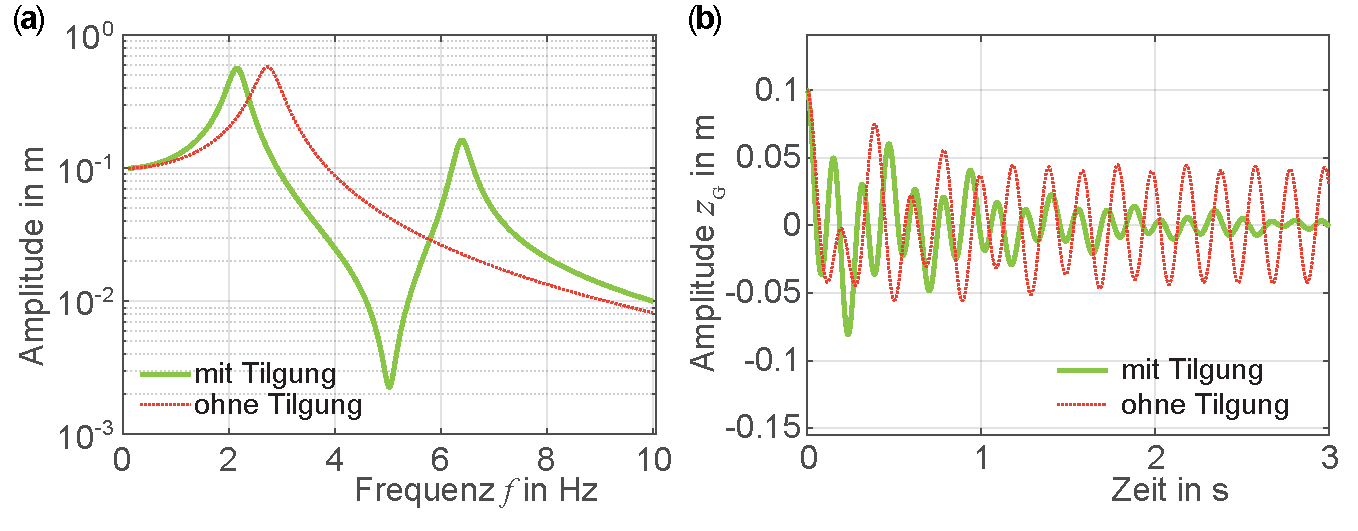
\includegraphics[width=\textwidth]{Tilgung04.pdf}%
\caption[Frequenzgang bei der Schwingungstilgung]{\fa Frequenzgang bei der Schwingungstilgung. Parameter: Masse Mikroskop $m_\text{G} =\SI{50.0}{\kg}$, 
Gegenmasse $m_\text{T} =\SI{25.0}{\kg}$, Federkonstante $k_\text{G} =\SI{15000.0}{\N\per\metre}$, Federkonstante $k_\text{T} =\SI{25000.0}{\N\per\metre}$, D�mpfung Ger�t $\eta_\text{G} =\SI{150.0}{\kg\per\s}$, D�mpfung Gegenmasse $\eta_\text{T}=\SI{100.0}{\kg\per\s}$, Eigenfrequenz Ger�t $f_\text{G}=\SI{2.76}{\per\s}$. Eigenfrequenz Gegenmasse $f_\text{T}=\SI{5.03}{\per\s}$. Man sieht, dass in dem gew�hlten Fall St�rfrequenzen bei 5 Hz optimal unterdr�ckt werden. Gleichzeitig treten aber bei $f \approx \SI{2.2}{\per\s}$ und $f \approx \SI{6.5}{\per\s}$ erhebliche Schwingungsverst�rkungen auf. \fb Einschwingverhalten der Schwingungstilgung bei den gew�hlten Parametern, \vgl \mlbewref{VibDaempfung02.m}}
\label{abb:bew_Tilgung03}
\end{figure}

In \figref{bew_Tilgung03}\,a sind die Amplitudeng�nge f�r die schwingenden
Massen $m_\text{G}$, $m_\text{G}$ nach \eqref{bew_tilgung09} und \eqref{bew_tilgung05}
dargestellt und zum Vergleich die Resonanzkurve einer Masse $m_\text{G}$,
die nur einer Federung mit der Konstanten $k_\text{G}$ unterliegt.
Man sieht sehr sch�n, dass durch die Schwingungstilgung mit der Masse $m_\text{T}$
die Amplitude der Masse $m_\text{G}$ in der Umgebung der Frequenz
$\omega_{0,T}=\sqrt{k_\text{T}/m_\text{T}-\text{T}}$ wirkungsvoll ged�mpft wird.\footnote{%
Man sieht aus \figref{bew_Tilgung03}\,a, dass es in benachbarten Frequenzbereichen durchaus
zu Verst�rkungen kommen kann. So wird zwar bei \SI{5}{\hertz} eine optimale D�mpfung erreicht, aber schon bei \SI{4}{\hertz} \bzw \SI{6}{\hertz} k�nnen gr��ere Auslenkungen beobachtet werden.} In \figref{bew_Tilgung03}\,b haben wir das Einschwingverhalten von $z_\text{G}(t)$ f�r eine Anregung bei \SI{5}{\hertz} mit und ohne Tilgung dargestellt.

	\subprob{Schwingungstilgung bei Hochh�usern}

\begin{figure}[H]\centering
\includegraphics[width=\textwidth]{Tilgung03.pdf}%
\caption[Prinzip des Gleitpendels und entsprechende Schwingungstilgung]{Prinzip des Gleitpendels. Hierin ist $m_\text{G}$ die effektiver Masse des Geb�udes, $m_\text{T}$ die Masse des Gegengewichts (Pendel), $L$ die Pendell�nge und $A_\text{ext}$ die externe Anregung. $k_\text{G}$ ist eine fiktive Federkonstante, die sich empirisch aus der Eigenfrequenz und der Masse des Hochhauses berechnen l�sst. F�r die Schwingungsperiode in Hochh�usern gilt folgende empirische N�herungsformel: $T ~\lek \text{in}~\SI{}{\second} \rek \approx H/46 \lek ~H~~\text{in}~\SI{}{\metre} \rek$.\\
F�r eine Prinziprechnung f�r die Dynamik des Gleitpendels wurde folgende exemplarische Parameter angenommen: $m_\text{G} =\SI{1.0}{\kg}$, $m_\text{T} =\SI{0.3}{\kg}$, $k_\text{G} =\SI{10.0}{\N\per\metre}$, L�nge Pendel $L =\SI{1.0}{\metre}$, D�mpfung Masse $\eta_\text{G} =\SI{0.6}{\kg\per\s}$, D�mpfung Gegenmasse $\eta_\text{T} =\SI{0.2}{\kg\per\s}$, Anregungskreisfrequenz $\omega =\SI{3.13}{\per\s}$, Anregungsamplitude $A_\text{ext} = \SI{0.10}{\metre}$, \vgl \mlbewref{Tilgung01.m}, \mlbewref{Tilgung02.m} und \mlbewref{Tilgung03.m}}
\label{abb:bew_Tilgung04}
\end{figure}

F�r Tilgung von Schwingungen in Hochh�usern gibt es zahlreiche Ausf�hrungsformen, die in vielen F�llen auf zwei mechanische Grundformen zur�ckgef�hrt werden k�nnen: 
\begin{enumerate}[a)]
  \item Ged�mpftes Pendel nach \figref{bew_Tilgung01}
  \item Gleitpendel nach \figref{bew_Tilgung04}\,a
\end{enumerate}

Wir k�nnten das Problem nach dem in Kap.~\ref{kap:bew_Tilgung} beschriebenen Verfahren l�sen, wollen hier aber das spezifische Problem der Gleitpendel-Ausf�hrung detaillierter betrachten. Wir �berlassen dem Leser den Fall a) nach \figref{bew_Tilgung01}. F�r das Gleitpendel k�nnen wir aus \figref{bew_Tilgung04}\,a die folgende Lagrange-Funktion bestimmen:
\begin{align}
  \mathcal{L}
  &=\underbrace{\frac {m_\text{G}}{2}\dot x^2+\frac {m_\text{T}}{2}\left(\dot x_\text{G}^2+L^2\dot\varphi^2+2L\dot\varphi\dot x_\text{G}\cos\varphi\right)}_{T} + \ldots \nonumber \\
	 &~~ - \underbrace{\lk m\,g\,L\,(1-\cos\varphi)+\frac {k_\text{G}}{2}\left(x_\text{G}-A_\text{ext}\sin(\omega t)\right)^2\rk}_{U}
  \label{bew_tilgung10}
\end{align}
Die Dissipationsfunktion $U_\text{R}$ (\vgl \kap{bew_Lagrange_II_R}) ist gegeben durch:
\begin{align}
  U_\text{R} = \frac{\eta_\text{G}}2\dot x_\text{G}^2+\frac{\eta_\text{T}}2\left(\dot x_\text{G}^2+L^2\dot\varphi^2+2L\dot\varphi\dot x_\text{G}\cos\varphi\right)\,.
  \label{bew_tilgung11}
\end{align}

Die Lagrange-Gleichungen berechnen sich dann zu:\\

\begin{align}
\begin{split}
    (m_\text{G}+m_\text{T})\ddot{x} &= -\lbrack k_\text{G}\,x + m_\text{T}\,L\,\ddot{\varphi}\,\cos\varphi - m_\text{T}\,L\,\dot{\varphi}^2\,\sin\varphi - \eta_\text{G}\,\dot{x} - \eta_\text{T}\, \lk \dot{x} + L\,\dot{\varphi}\,\cos\varphi \rk \rbrack \\ & \quad  ~~ + k_\text{G}\,A_\text{ext}\,\sin(\omega t)  \\  \label{eq:bew_GleitP01}
    m_\text{T}\,L\,\ddot{\varphi} &= -m_\text{T}\,\lek \ddot{x}\,\cos\varphi + g\,\sin\varphi\rek - \eta_\text{T}\,\lk \dot{x}_{\cos\varphi} + L\,\dot{\varphi}\rk \;.
\end{split} 
\end{align}
Wir k�nnen f�r kleine $\varphi$, $x$ die beiden Gleichungen linearisieren und setzen die zweite in die erste ein, womit wir erhalten:
\begin{align}
\begin{split}
    \ddot{x} &= -\frac{1}{m_\text{G}+m_\text{T}}\,\lek k_\text{G}\,x + m_\text{T}\,L\,\ddot{\varphi} + \eta_\text{G}\,\dot{x} + \eta_\text{T}\lk \dot{x} + L\,\dot{\varphi} \rk - k_\text{G}\,A_\text{ext}\,\sin(\omega t)\rek \\
    m_\text{T}\,L\,\ddot{\varphi} &= -m_\text{T}\,\lek \ddot{x} + g\,\varphi \rek - \eta_\text{T}\,\lk \dot{x} + L\,\dot{\varphi}\rk \,.
  \end{split} \label{eq:bew_GleitP03}
\end{align}
Wir erhalten dann f�r $\ddot{x}$ und $\ddot{\varphi}$
\begin{align}
\begin{split}
  \ddot{x} &= -\frac{1}{m_\text{G}}\,\lek k_\text{G}\,x -m_\text{T}\,g\,\varphi + \eta_\text{G}\,\dot{x} - k_\text{G}\,A_\text{ext}\,\sin(\omega t)\rek \, \\
  \ddot{\varphi} = &+\frac{1}{m_\text{G}\,L}\,\lek k_\text{G}\,x m_\text{T}\,g\,\varphi + \eta_\text{G}\,\dot{x}  - k_\text{G}\,A_\text{ext}\,\sin(\omega t)\rek - \lek \frac{\eta_\text{T}}{m_\text{T}\,L}\,\lk \dot{x} +L\,\dot{\varphi}\rk + \frac{g}{L}\,\varphi \rek \,.
\end{split} \label{eq:bew_GleitP04}
\end{align}

Die numerische L�sung erfolgt in \mlbewref{Tilgung03.m} und ist in \figref{bew_Tilgung04}b gezeigt. Aus der Abbildung erkennt man sehr sch�n, dass das Pendel die schwingende Masse sehr effektiv d�mpft und dass die Pendelschwingung der Schwingung der Hauptmasse um etwa $\pi/2$ nacheilt. Durch diese Phasenverschiebung zwischen den beiden Schwingungen kommt letztendlich die effektive D�mpfung zustande. Ein Problem bei der gew�hlten Auslegung ist, dass das Pendel relativ stark ausgelenkt wird ($\approx 45\degree$)  und eigentlich unsere lineare N�herung schon nicht mehr gilt. Au�erdem stellt eine solch starke Auslenkung an die Baukonstruktion erhebliche Anforderungen. Wie diese gel�st wurden, kann man sich \zb bei dem Geb�ude $101$ in Taipei oder dem Berliner Fernsehturm ansehen (siehe auch \cite{Ucke2008}).\\ 

Wir haben einige Werte und Absch�tzungen (in rot) aus unserem Modell in der Tabelle \ref{tab:bew_hihrises} zusammengefasst und sind dabei folgenderma�en vorgegangen:
\begin{enumerate}
	\item Annahmen
	\begin{align*}
    \eta_\text{G}= 0\,,~~~~~ \omega_\text{G}{}^2 = \frac{k_\text{G}}{\lk m_\text{G}+m_\text{T}\rk}\,,~~~~~~ \frac{m_\text{T}}{m_\text{G}}=\gamma\,,~~~~~~~~ \eta_\text{G} \neq 0\,,~~~~~~ \omega_\text{T}{}^2=\frac{g}{L}\,.
\end{align*}
\item F�r die L�sung des DGL-Systems \eqref{eq:bew_GleitP03} machen wir folgenden Ansatz:
\begin{align*}
    x &= \hat{X}\,\e^{\im\omega t}\,,~~~~~~~~   \varphi = \hat{\phi}\,\e^{\im\omega t}\,,~~~~~~~~   F = \underbrace{k_\text{G}\,A_\text{ext}}_{\substack{F_x}}\,\e^{\im\omega t}\,,  \\
    \rightarrow ~ \hat{F}_\text{ext} &=  -\omega^2\,\hat{X} + \frac{k_\text{G}}{m_\text{G}+m_\text{T}}\,\hat{X} + \frac{m_\text{T}}{m_\text{G}+m_\text{T}}\,L\,\hat{\phi}\,\lk -\omega^2\rk + \im\omega\frac{\eta_\text{T}}{m_\text{G}+m_\text{T}}\,\lk \hat{X} + L\,\hat{\phi}\rk \,.
\end{align*}
\item Es ergibt sich folgendes lineares Gleichungssystem: 
\begin{align*}
    \hat{X}\,\underbrace{\lk -\omega^2 + \omega_\text{G}{}^2 + \im\omega\,\frac{\eta_\text{T}}{m_\text{G}+m_\text{T}}\rk}_{A} + \hat{\phi} \underbrace{\lk-\frac{\gamma}{1+\gamma}\,L\,\omega^2 + \im\omega\,\frac{L\,\eta_\text{T}}{m_\text{G}+m_\text{T}}\rk}_{B} &= \ldots \\
		\frac{k_\text{G}\,A_\text{ext}}{m_\text{G}+m_\text{T}} = \omega_\text{G}{}^2\,A_\text{ext} &= \hat{F}_\text{ext}\,,\\
    \hat{X}\,\underbrace{\lk -\frac{\omega^2}{L} + \im\omega\,\frac{\eta_\text{T}}{m_\text{T}\,L}\rk}_{C} + \hat{\phi} \underbrace{\lk  -\omega^2 + \omega_\text{T}{}^2 + \im\omega\,\frac{\eta_\text{T}}{m_\text{T}}\rk}_{D}  &= 0 \,.
\end{align*}
\item Wir l�sen das lineares Gleichungssystem nach $\hat{X}$: 
\begin{align*}
    \hat{X}\,A + \hat{\phi}\,B &= \hat{F}_\text{ext} ~ ~\big| \cdot D \,,~~~~~~ \hat{X}\,C + \hat{\phi}\,D = 0 ~~ \big| \cdot B  \\
    \rightarrow ~~~~ \hat{X}  &= \frac{\hat{F}_x\,D}{AD-BC} 
\end{align*}
mit
\begin{align*}
    A&= -\omega^2 + \omega_\text{G}{}^2 + \frac{\im\omega\,\eta_\text{T}\,\gamma}{m_\text{T}\,\lk 1+\gamma\rk}\,, & C&= -\frac{\gamma}{1+\gamma}\,L\,\omega^2 + \frac{\im\omega\,\gamma}{m_\text{T}\,\lk 1+\gamma\rk}\,L\,\eta_\text{T}\,,\\
    B&= -\frac{\omega^2}{L} + \frac{\im\omega\,\eta_\text{T}}{m_\text{T}}\,\frac{1}{L}\,, & D&= -\omega^2 + \omega^2 + \im\omega\,\frac{\eta_\text{T}}{m_\text{T}}\,.
\end{align*}
\item Die Frequenzantwort $R\lk\omega\rk$ ist dann gegeben durch 
\begin{align*}
    R\lk\omega\rk = \Big| \frac{\hat{X}}{\omega_\text{G}{}^2\,A_\text{ext}}\Big|
\end{align*}
und in {\figref{bew_Tilgung05}} gezeigt.
\end{enumerate}
\begin{table}%tab
\centering
\caption{Vergleich von Schwingungstilgungen am Geb�ude 101 in Taipei und am Berliner Fernsehturm}
\smallskip
\begin{tabular}{L{4.5cm}L{2.2cm}L{1cm}L{1.8cm}L{1.8cm}}
Physikalische Gr��e	&	 Symbol & Einheit & Taipei 101 & Fernsehturm Berlin \\ \\
\noalign{\smallskip}\hline\noalign{\smallskip}
\smallskip
& & \\
Relevante H�he (ohne Antenne)	&$ H $& m & 448 & 210\\
Eigenfrequenz Geb�ude &$ \omega_M $& \SI{}{\per\second} & 0.628 & 1.257\\
Schwingungsperiode Geb�ude &$ T_M$& \SI{}{\second} &12.5 & 5.5 \\
Masse	Pendel &$ m_\text{T}$& kg & \SI{662e3}{}& \SI{1.5e3}{} \\
\textcolor{blue}{Masseverh�ltnis (angenommen)} &$ \gamma $& &\textcolor{red}{0.05} & \textcolor{red}{0.05}\\
L�nge	Pendel &$ L $& m & \SI{42.0}{} & \SI{5}{}\\
Eigenfrequenz Pendel &$ \omega_\text{T} $& \SI{}{\per\second} &0.48 & 0.22\\
\textcolor{blue}{D�mpfung Pendel (berechnet)}&$\eta_\text{T}$ & $ \SI{}{\kg\per\second}$ &\textcolor{red}{$\SI{5.0e3}{}$} & \textcolor{red}{25}\\
\textcolor{blue}{Auslenkung mit Tilgung (berechnet)} & $R(\omega)A_\text{ext}$ & $\SI{}{\metre}$ & \textcolor{red}{1.4} & \textcolor{red}{0.13} \\
\textcolor{blue}{max. Beschleunigung mit Tilgung}& $R(\omega)A_\text{ext}\,\omega_\text{T}{}^2$ & $\SI{}{\metre\per\second\squared}$ & \textcolor{red}{0.33} & \textcolor{red}{0.25}\\ 
\noalign{\smallskip}\hline\noalign{\smallskip} \\
\noalign{(In blau angemommene bzw. berechnete Gr��en.)}\\
\end{tabular}\\ 
\label{tab:bew_hihrises}
\end{table}
\begin{figure}[H]\centering
\includegraphics[width=\textwidth]{Tilgung05.pdf}%
\caption[Frequenzantwort des Geb�udes Taipei 101 und des Berliner Fernsehturms]{Modellierung Frequenzantwort des Geb�udes Taipei 101 \fa und des Berliner Fernsehturms \fb . Parameter siehe Tab. \ref{tab:bew_hihrises}} \label{abb:bew_Tilgung05}
\end{figure}

\end{subprobs}
\medskip

\end{sol} 
\textcolor{blue} {$\rightarrow$ zur} \probref{bew_Stossdaempfer}.\\
\noindent\rule[1ex]{\textwidth}{0.5pt}  \newpage

\newpage

\begin{sol}{prob:bew_PendelUeb02}\label{lsg:bew_PendelUeb02} %�bung31
\textbf{Blackwood Pendel, Ballistisches Pendel.} \\ \\
Das Geschoss habe die Geschwindigkeit $v_\text{G}$, die es zu bestimmen gilt und eine Masse $m_\text{G}$, die bekannt ist. Der schwere Holzblock mit der Masse $m_\text{B}$ h�ngt in Ruhe an einer Aufh�ngung der L�nge $L$. \\
Die Maximalauslenkung $\varphi_\text{max}$ wird gemessen. \\
Aus der Energieerhaltung folgt:
\begin{align*}
    U\lk\varphi_\text{max}\rk &= T\lk \varphi=0\rk \\
    \lk m_\text{G}+m_\text{B}\rk\,g\,\Delta z &= \frac{\lk m_\text{G}+m_\text{B}\rk}{2}\,{v_0}^2 \\
\end{align*}
Aus dem Impulssatz folgt:
\begin{align*}
    m_\text{G}\,v_\text{G} &= \lk m_\text{G}+m_\text{B}\rk\,v_0 \\
    v_0 &= \frac{m_\text{G}}{m_\text{G}+m_\text{G}}\,v_\text{G}
\end{align*}
Damit erhalten wir:
\begin{align*}
    g\,L\,\lk 1-\cos\,\varphi_\text{max}\rk &= \frac{1}{2} \lk \frac{m_\text{G}}{m_\text{G}+m_\text{B}}\,v_\text{G}\rk^2 \\
    g\,L\,\lk 1-\cos\varphi_\text{max}\rk &= \frac{{m_\text{G}}}{m_\text{G}+m_\text{B}}\,\frac{{v_\text{G}}^2}{2}
\end{align*}
\begin{align*}
    \rightarrow v_\text{G} = \sqrt{2g\,L\,\lk 1-\cos\varphi_\text{max}\rk}\,\lk 1+\frac{m_\text{B}}{m_\text{G}}\rk
\end{align*}

\end{sol} 
%\href{PhysikUncut_Part1.pdf#prb:bew_PendelUeb02}{\textcolor{blue} {$\rightarrow$ zur \probref{bew_PendelUeb02}.}}\\
\textcolor{blue} {$\rightarrow$ zur} \probref{bew_PendelUeb02}.\\
\noindent\rule[1ex]{\textwidth}{0.5pt}  \newpage


%-----------------------------------------------------------------------------------------------------------
\hypertarget{lsg:bew_PendelUeb04}{}
\begin{sol}{prob:bew_PendelUeb04}\label{lsg:bew_PendelUeb04} %�bung32
\textbf{Wilberforce-Pendel.} \\ \\
Wilberforce zeigte bereits 1895, dass eine Feder mit einer verbundenen zylindrischen Masse L�ngs- und Drehschwingungen ausf�hrt und diese gekoppelt sind. Sommerfeld gab als erster eine umfassende theoretische Beschreibung. Seine Herleitung der Bewegungsgleichungen beruhte auf Prinzipien der Differential\-geometrie. In der ausgezeichneten Arbeit \cite{Koepf1990} wird eine detaillierte Herleitung aus elastomechanischen �berlegungen gegeben. Wir werden hier nur das Ergebnis, d.h. die abgeleitete Lagrange-Gleichung verwenden und empfehlen dem interessierten Leser die Herleitung in \cite{Koepf1990} im Kapitel \ref{kap:kontmech_uebungen} nachzuvollziehen.\\
Die zun�chst �berraschende Eigenschaft des Wilberforce-Pendels resultiert aus einer Kopplung der zwei Bewegungen aufgrund der Geometrie der Feder. Wenn sich die Masse auf und ab bewegt, f�hrt jede Abw�rtsbewegung zu einer leichten Abwicklung der Feder, wodurch die Masse ein kleines Drehmoment erf�hrt. Eine Aufw�rtsbewegung der Masse dagegen l�sst die Windungszahl der Feder, d.\,h. die Zahl der Windungen pro L�nge leicht ansteigen und gibt damit der Masse ein kleines Drehmoment in die andere Richtung. Jede Auf- und Abschwingung f�hrt also zu einem Drehmoment und damit wird mit jeder Schwingung Energie von der Vertikalschwingung in die Torsionsschwingung �bertragen, sodass die Amplitude der Torsionsschwingung anw�chst und gleichzeitig die der Vertikalschwingung abnimmt.
Unter der Annahme einer linearen Kopplung zwischen diesen beiden Schwingungen
kann die Lagrange-Funktion geschrieben werden als
\begin{align}
    \mathcal{L} = \frac{1}{2}\,m_\text{F}\,\dot{z}^2 + \frac{1}{2}\,J_\text{T}\,\dot{\varphi}^2 - \frac{1}{2}\,k_\text{F}\,z^2-\frac{1}{2}\,D_\text{T}\,\varphi^2-\frac{1}{2}\,\kappa\,z\,\varphi \,, \label{eq:bew_wilberforce02}
 \end{align}
wobei der Kopplungskoeffizient mit $\kappa$ bezeichnet wurde und die Indizes F \bzw T sich jeweils auf die vertikale Federschwingung \bzw die horizontale Torsionsschwingung beziehen. 
F�gt man nun geschwindigkeitsproportionale Reibung, parametriert durch die Reibungskoeffizienten $\eta_\text{F}$ bzw. $\eta_\text{T}$, hinzu und ersetzt $\omega_\text{F}{}^2 = k_\text{F}/m_\text{F}$ und $\omega_\text{T}{}^2 = D_\text{T}/J_\text{T}$, so erh�lt man 
%Aus \eqref{eq:bew_wilberforce02} folgen dann mit $\omega_\text{F}{}^2 = k_\text{F}/m_\text{F}$ und $\omega_\text{T}{}^2 = D_\text{T}/J_\text{T}$ und den hinzugef�gten Reibungstermen $\eta_\text{F}$ bzw. $\eta_\text{T}$ 
die Bewegungsgleichungen f�r die gekoppelten Oszillatoren des Wilberforce-Pendels:
\begin{align}
    \begin{split}
        \ddot{z}  + {\omega_\text{F}}^2\, z +\frac{1}{2}\frac{\kappa}{m_\text{F}}\,\varphi 
			          	+ \frac{\eta_\text{F}}{m_\text{F}}\,\dot{z} &= 0 \,,\\
        \ddot{\varphi} + {\omega_\text{T}}^2\,\varphi + \frac{1}{2}\frac{\kappa}{J_\text{T}}\, z 
				          + \frac{\eta_\text{T}}{J_\text{T}}\,\dot{\varphi} &= 0\,.
    \end{split} \label{eq:bew_wilberforce03}
\end{align}
Aus \eqref{eq:bew_wilberforce03} kann man (etwas vereinfachend formuliert) ablesen: Die longitudinale Eigenfrequenz der Feder ist durch $\omega_\text{F}=\sqrt(k_\text{F}/m_\text{F})$ gegeben, die Eigenfrequenz der Rotationsschwingung durch $\omega_\text{T}=\sqrt(D_\text{T}/J_\text{T})$. Wenn beide Eigenfrequenzen �bereinstimmen ($\omega_\text{F}\approx\omega_\text{T}$), kommt es zur Resonanz und zum ausgepr�gten "`Hin- und Herschaukeln"' der Energie (\figref{bew_wilberforce02}). Die Resonanzabstimmung kann man mit einer Fein\-abstimmung der Massen auf der Torsionsstange erreichen. Bei gro�er Verstimmung oder auch starker Reibung verschwindet jedoch der Oszillationseffekt der Energie.\\
Wir haben diese Art von gekoppelten DGL bereits in Kapitel \ref{kap:bew_pendulum_coupled} sowohl im Kleinwinkelverhalten, als auch mit der Methode der Normalmoden untersucht. Wir wollen zun�chst aber auf die numerische Behandlung zur Berechnung des zeitlichen Verhaltens des Pendels und der Energie unter L�sung des Gleichungssystem \eqref{eq:bew_wilberforce03} eingehen.
F�r eine folgende numerische Berechnung wollen wir das Gleichungssystem \eqref{eq:bew_wilberforce03} gleich um  einen Antrieb ($A_\text{F}, B_\text{T}, \omega$) und weitere durch Reibungseffekte motivierte nichtlineare Terme ($\epsilon_\text{F}\,\omega_\text{F}{}^2\,z^3$ \bzw $\epsilon_\text{T}\,\omega_\text{T}{}^2\,\varphi^3$) erweitern. 
Wir erhalten dann aus \eqref{eq:bew_wilberforce03}: 
\begin{align}
   \begin{split}
      \ddot{z} + {\omega_\text{F}}^2\,\lk z + \epsilon_\text{F}\,z^3 \rk 
			         + \frac{1}{2}\frac{\kappa}{m_\text{F}}\,\varphi 
			         + \frac{\eta_\text{F}}{m_\text{F}}\,\dot{z}  
							&= A_{\text{F}}\,\sin\omega t\,,  \\
      \ddot{\varphi} + {\omega_\text{T}}^2\, \lk \varphi + \epsilon_\text{T}\,\varphi^3 \rk 
			         + \frac{1}{2}\frac{\kappa}{J_\text{T}}\,z +  \frac{\eta_\text{T}}{J_\text{T}}\,\dot{\varphi} 
							&= B_\text{T}\,\sin\omega t \,.
    \end{split} \label{eq:bew_wilberforce04}
\end{align} 

Wir benutzen f�r die numerischen Rechnungen die Parameter, die ann�hernd dem Wilberforce-Pendel der Fa. Leybold-Didactic entsprechen (Tabelle \ref{tab:bew_wilberforce}) und erhalten die in \figref{bew_wilberforce02} dargestellte zeitliche Dynamik des Schraubenpendels. Man erkennt deutlich das Hin- und Herpendeln der Energie von der Federschwingung auf die Torsionsschwingung.

\begin{figure}[H]\centering
\includegraphics[width=\textwidth]{Wilberforce01.pdf}
\caption[Dynamik des linearen Wilberforce-Pendels (Schwingende Schraubenfeder)]
{Dynamik des linearen Wilberforce-Pendels (Schwingende Schraubenfeder) im Resonanzfall nach \eqref{eq:bew_wilberforce03}. \fa Entwicklung von $z(t)$ und $\varphi(t)$, \fb Energien der Feder $E_\text{F}(t)$ und des Torsionspendels $E_\text{T}(t)$ nach \eqref{eq:bew_wilberforce03}, Parameter siehe Tab. \ref{tab:bew_wilberforce} und  \mlbewref{Wilberforce.m}}
\label{abb:bew_wilberforce02}
\end{figure}

\begin{table}[h!]
\caption{Wesentliche Parameter des Wilberforce-Pendels\cite{Berg1991}}
    \begin{tabular}{L{1.5cm}L{3cm}L{5cm}}
         $m_\text{F}$&$\SI{0.5164}{\kg}$& Masse Federpendel  \\
         $k_\text{F}$&$\SI{2.8}{\newton\per\metre}$& Federkonstante \\
         $L_\text{F}$&$\SI{1.765}{\metre}$& L�nge Feder \\
			   $\omega_\text{F}$&$\SI{2.3286}{1\per\second}$& Eigenfrequenz Feder \\ \\
         %$R_\text{H}$&$\SI{0.015}{\metre}$& Durchmesser der Helix der Feder \\
         %$n$&$125$&  Windungszahl\\ 
         %$\alpha$&$\atan\lk\frac{L_\text{F}}{2\pi\,R_\text{H}\,n}\rk = \SI{0.149}{\radian}$\:& Anstiegswinkel \\         
				 $m_\text{T}$&$\SI{0.418}{\kg}$&  Masse Torsionsgewicht\\
         $J_\text{T}$&$\SI{1.45e-04}{\kg\metre\squared}$ & Tr�gheitsmoment der Torsionsstange   \\
         $D_\text{T}$&$\SI{7.86e-04}{\newton\metre\per\radian}$ & Torsionsmoment \\
				 $\omega_\text{T}$&$\SI{2.3384}{1\per\second}$& Eigenfrequenz Torsionsstange  \\	\\
         $\kappa $&$ \SI{2.73e-03}{\N\per\radian}$& Kopplungskonstante\\
	       $\epsilon_\text{F} $&$ 0.00 \ldots 0.05$& Nichtlinearit�t Feder \\			
	       $\epsilon_\text{T}$&$ 0.00 \ldots 0.02$&Nichtlinearit�t Torsionsstange	\\		
    \end{tabular} 
\end{table} \label{tab:bew_wilberforce}

Als Erweiterung kann man die zeitliche Entwicklung von $\varphi\lk t\rk$ und $z\lk t\rk$ f�r ein nichtlineares, getriebenes Wilberforce-Pendel mit Nichtlinearit�ten ($\epsilon_\text{F} \neq 0$ \bzw $\epsilon_\text{T} \neq 0$) berechnen, vgl. auch \mlbewref{Wilberforce.m}. Man kann zeigen, dass je nach Gr��e der Nichtlinearit�t 
%$\epsilon_\text{F}$ \bzw $\epsilon_\text{T}$ 
die Frequenzen der Schwebung zwischen Feder und Torsionsstange zu kleineren \bzw gr��eren Werten hin \anf{verschoben} werden. Bei bestimmten Verh�ltnissen kann es sogar zu einer Verdopplung der Schwingungsdauer kommen (\figref{bew_wilberforce03}), einem typischen Ph�nomen nichtlinearer Systeme (siehe Kapitel \ref{kap:bew_chaos}).

\begin{figure}[H]\centering
\includegraphics[width=\textwidth]{Wilberforce02.pdf}
\caption[Dynamik f�r das nichtlineare Wilberforce-Pendel .]{Dynamik f�r das nichtlineare Wilberforce-Pendel im Resonanzfall nach \eqref{eq:bew_wilberforce04}. \fa Darstellung von $z(t)$ und $\varphi(t)$ und \fb der Energien von Feder- und Torsionspendel nach \eqref{eq:bew_wilberforce04}, Parameter siehe Tab. \ref{tab:bew_wilberforce} und \mlbewref{Wilberforce.m}, die Reibung wurde vernachl�ssigt und die Nichtlinearit�tskoeffizienten betragen $\epsilon_\text{F}=0.03$ \bzw $\epsilon_\text{T}=0$}\label{abb:bew_wilberforce03}
\end{figure}

Eine Variation des Wilberforce-Pendels ist das Valett-Pendel \cite{Ucke2021}, bei dem sowohl am oberen als auch am unteren Ende der Feder eine Torsionsstange angebracht ist. 
Wir verweisen dazu auf die Referenzen \cite{Koepf1990, Berg1991}, in denen die Aufstellung der Lagrange-Funktion \bzw Lagrange-Gleichungen f�r das Wilberforce-Pendel behandelt wird,  die auf Sommerfeld\indexp{Sommerfeld, Arnold} zur�ck geht. Ganz analog kann man die Differentialgleichungen f�r ein Valett-Pendel aufstellen, wobei wir in diesem Fall drei generalisierte Koordinaten ($z,\, \varphi_1,\, \varphi_2$) haben. Interessant ist, dass bei diesem Pendel, das Auf- und Abwickeln der Feder mit einer jeweils entgegengesetzten Drehung der Torsionstangen am oberen und unteren Ende verbunden ist. Wir verweisen auf  die Zusatzaufgabe in \probref{bew_Zusatz_ValletPendel}.\\

Wir wollen jetzt noch kurz die Vorgehensweise f�r die analytische Berechnung skizzieren und folgen dabei \cite{Berg1991}.\\
Wir starten wieder von \eqref{eq:bew_wilberforce03} (ohne Reibungsterme) und leiten die zweite Gleichung noch zweimal nach der Zeit ab. Wir substituieren $\ddot{z}$ durch die erste Gleichung und erhalten nach einigen Umformungen:
\begin{align}
\frac{\D^4 \varphi}{\D t^4} + \lk \omega_\text{F}{}^2+\omega_\text{T}{}^2 \rk \frac{\D^2 \varphi}{\D t^2}
+ \lk \omega_\text{F}{}^2\omega_\text{T}{}^2 - \frac{\kappa^2}{4\,m_\text{F}\, J_\text{T}}\rk \, \varphi = 0\,.
\label{eq:bew_wilberforce05} 
\end{align} 
Mit dem Ansatz $\varphi(t) = Q\,\e^{\im\omega t}$ findet man die charakteristische Gleichung 
\begin{align}
 \omega^4 - (\omega_\text{F}{}^2 +\omega_\text{T}{}^2) \omega^2 + \lk \omega_\text{F}{}^2\omega_\text{T}{}^2 - \frac{\kappa^2}{4\,m_\text{F}\, J_\text{T}}\rk = 0\,,
\label{eq:bew_wilberforce06}
\end{align}
deren L�sungen lauten:
\begin{align}
 \omega_{1,2}{}^2 &= \frac{1}{2} \lek \omega_\text{F}{}^2 + \omega_\text{T}{}^2 \pm \sqrt{\lk \omega_\text{F}{}^2 - \omega_\text{T}{}^2\rk^2 + \frac{\kappa^2}{\,m_\text{F}\, J_\text{T}}} \rek \,.
\label{eq:bew_wilberforce07}
\end{align} 
F�r den Resonanzfall $\omega_\text{F} = \omega_\text{T} = \omega_0$ ergibt sich:
\begin{align*}
	 \omega_{1,2}{}^2 &= \omega_0{}^2 \pm \frac{1}{2}\sqrt\frac{\kappa^2}{m_\text{F}\, J_\text{T}}\,.
\end{align*}
Wir f�hren die Schwebungsfrequenz
\begin{align}
     \omega_\text{S} = \frac{\kappa}{ 2\omega_0\sqrt{\,m_\text{F}\, J_\text{T}}}\, \label{eq:bew_wilberforce08}
\end{align}
ein und erhalten f�r den Fall, dass $\omega_\text{S} \ll \omega_0$ 
\begin{align}
	 \omega_{1,2} \approx \omega_0 \pm \frac{1}{2}\,\omega_\text{S} = \omega_0 \pm \frac{\kappa}{4\omega_0\sqrt{\,m_\text{F}\, J_\text{T}}} \,. \label{eq:bew_wilberforce08a}
\end{align}

Wir haben damit die Frequenzen $\omega_1$ und $\omega_2$ der beiden Normalmoden hergeleitet. Die Gesamtbewegung des Pendels (\zb des Endpunktes einer Torsionsstange der L�nge $2 l_\text{T}$) kann beschrieben werden durch
\begin{align}
	\vec{X}(t) = z(t)\,\veceZ + l_\text{T}\,\varphi(t)\,\vec{e}_\varphi \,,
  \label{eq:bew_wilberforce09}
\end{align}
worin noch $z(t)$ und $\varphi(t)$ zu bestimmen sind. F�r $\varphi(t)$ und damit $\ddot{\varphi}(t)$ k�nnen wir ansetzen:
\begin{subequations}
\begin{align}
	 \varphi(t) &= A\sin\omega_1 t + B\cos\omega_1 t + C\sin\omega_2 t + D\cos\omega_2 t\,,  \\
	 \ddot{\varphi}(t) &= -\omega_1{}^2\,A\sin\omega_1 t  -\omega_1{}^2\,B\cos\omega_1 t  -\omega_2{}^2\,C\sin\omega_2 t  -\omega_2{}^2\,D\cos\omega_2 t\,.  
\end{align} 	\label{eq:bew_wilberforce10}
\end{subequations}

Wir setzen \eqref{eq:bew_wilberforce10} in \eqref{eq:bew_wilberforce04} ein und erhalten $z(t)$ und auch $\ddot{z}$. Mit den Anfangsbedingungen, $z(0)=z_0\neq 0,\, \varphi(0) = \varphi_0 \neq 0$ und allen  Anfangsgeschwindigkeiten gleich Null sind dann $A, C = 0$ und $B,\, D$ bestimmen sich aus $z_0,\, \varphi_0$\;.
Wir erhalten damit folgenden L�sungen:
\begin{subequations}
\begin{align}
	z(t) &= z_0\,(\omega_1{}^2-\omega_2{}^2)^{-1}\, 
	        \lek (\omega_1{}^2-\omega_\text{T}{}^2)\,\cos\omega_1 t - (\omega_2{}^2-\omega_\text{T}{}^2)                 \,\cos\omega_2 t \rek \nonumber\\
					&- \frac{2J_\text{T}\varphi_0}{\kappa}\,(\omega_1{}^2-\omega_2{}^2)^{-1} \,  
					      (\omega_1{}^2-\omega_\text{T}{}^2)\,  (\omega_2{}^2-\omega_\text{T}{}^2)\,
								(\cos\omega_1 t - \cos\omega_2 t)\,.\\
\varphi(t) &= \frac{\kappa\,z_0}{2J_\text{T}}\,(\omega_1{}^2-\omega_2{}^2)^{-1}\,
                                               (\cos\omega_1 t - \cos\omega_2 t)\,\nonumber \\
	       & + \varphi_0 \,(\omega_1{}^2-\omega_2{}^2)^{-1} 
					   \lek (\omega_1{}^2-\omega_\text{T}{}^2)\,\cos\omega_2 t - (\omega_2{}^2-\omega_\text{T}{}^2)                 \,\cos\omega_1 t \rek \,.
\end{align}   \label{eq:bew_wilberforce11}
\end{subequations}

Damit k�nnen jetzt die Normalkoordinaten bestimmen (\vgl \kap{bew_pendulum_coupled}):
\begin{align}
	\vec{X}(t) &= z(t)\,\veceZ + l_\text{T}\,\varphi(t)\,\vec{e}_\varphi \nonumber \\
	           &= N_\text{n, 1} \cos\omega_1 t\, \vec{n}_1 + N_\text{n, 2} \cos\omega_2 t\, \vec{n}_1\,,
  \label{eq:bew_wilberforce12}
\end{align}
worin die $\vec{n}_i$ die Normalvektoren und die $N_\text{n, i}$ ihre Amplituden sind. 
Man bestimmt leicht
\begin{subequations}
\begin{align}
	\vec{n}_1 &= l_\text{T}\,\vec{e}_\varphi + \frac{2J_\text{T}}{\kappa}\,(\omega_1{}^2-\omega_\text{T}{}^2)\,\veceZ \,\\
	\vec{n}_2 &= l_\text{T}\,\vec{e}_\varphi + \frac{2J_\text{T}}{\kappa}\,(\omega_2{}^2-\omega_\text{T}{}^2)\,\veceZ \,\\
  N_\text{n, 1} &= +(\omega_1{}^2-\omega_2{}^2)^{-1}\,\lek \frac{\kappa\,z_0}{2J_\text{T}} 
	                  - (\omega_2{}^2-\omega_\text{T}{}^2)\,\varphi_0 \rek \,\\
  N_\text{n, 2} &= -(\omega_1{}^2-\omega_2{}^2)^{-1}\,\lek \frac{\kappa\,z_0}{2J_\text{T}} 
	                  - (\omega_2{}^2-\omega_\text{T}{}^2)\,\varphi_0 \rek \,,
\end{align} \label{eq:bew_wilberforce13}
\end{subequations}

wobei wir $l_\text{T}$ eingef�gt haben, damit die Normalenvektoren die Dimension L�nge haben. Will man nur eine der Normalmoden anregen, \zb die mit Frequenz $\omega_1$, dann muss $N_\text{n, 2}=0$ sein, woraus folgt 
	\[z_0=\sqrt{\frac{J_\text{T}}{m_F}}\, \varphi_0\,,
\]
also eine Bedingung f�r die Anfangswerte $z_0,\, \varphi_0$. Wir verweisen auf das \mscr{} \mlbewref{Wilberforce.m}.

\begin{figure}[H]\centering
\includegraphics[width=\textwidth]{Wilberforce03.pdf}
\caption[Dynamik des linearen Wilberforce-Pendels nach analytischer und numerischer Rechnung]
{Dynamik des linearen Wilberforce-Pendels nach analytischer und numerischer Rechnung im Resonanzfall nach  \eqref{eq:bew_wilberforce11}. \fa Vergleich der zeitlichen Entwicklung von $z(t)$ und $\varphi(t)$ nach analytischer und numerischer Rechnung nach \eqref{eq:bew_wilberforce11}. \fb Entstehende Normalschwingung $\omega_1$ nach \eqref{eq:bew_wilberforce13} bei der Anfangsbedingung $z_0 = \SI{0.005}{\metre},\, \varphi_0 = \sqrt{m_F/J_\text{T}} = \SI{0.3}{}\pi$, weitere Parameter siehe Tab. \ref{tab:bew_wilberforce} und \mlbewref{Wilberforce.m}}
\label{abb:bew_wilberforce04}
\end{figure}

\end{sol} 
%\href{PhysikUncut_Part1.pdf#prb:bew_PendelUeb04}{\textcolor{blue} {$\rightarrow$ zur \probref{bew_PendelUeb04}.}}\\
\textcolor{blue} {$\rightarrow$ zur} \probref{bew_PendelUeb04}.\\
\noindent\rule[1ex]{\textwidth}{0.5pt}  \newpage

%-----------------------------------------------------------------------------------------------------------

%%%-----------------------------------------------------------------------------------------------------------
%%%-----------------------------------------------------------------------------------------------------------


\subsection{�bungen zu nichtlinearen und komplexen Systemen}
\medskip

%-----------------------------------------------------------------------------------------------------------
\hypertarget{lsg:bew_logisticmap}{}
\begin{sol}{prob:bew_logisticmap}\label{lsg:bew_logisticmap} %�bung33
\textbf{Logistische Gleichung -- Populationsproblem.}\\ \\
Die Berechnungen sind in den \mscren\mlbewref{LogistischeGleichung01.m} und \mlbewref{LogistischeGleichung02.m} ausgef�hrt und in den \figref{bew_logisticmap01} und \figref{bew_logisticmap02} gezeigt.
Man erkennt folgende Charakteristika:

\begin{figure}[H]\centering
\includegraphics[width=\textwidth]{LogisticMap01.pdf}
\caption[Entwicklung der Populationen nach der Logistischen Gleichung]{Entwicklung der Populationen nach der Logistischen Gleichung f�r verschiedene Gr��en des Wachstumsparameters $\Gamma$}
\label{abb:bew_logisticmap01}
\end{figure}

Bei verschiedenen $\Gamma$ k�nnen wir folgende Verhaltensweisen f�r $k\rightarrow\infty$ beobachten.
Das Verhalten h�ngt nicht vom Anfangswert $x_1$ ab, sondern nur von $\Gamma$:
\begin{enumerate} [a)]
\item $0 < \Gamma < 1$ : Die Population stirbt aus.
\item $1 < \Gamma < 2$ : Die Population n�hert sich monoton dem Grenzwert $\frac {\Gamma-1}{\Gamma}$ an.
\item $2 < \Gamma < 3$ : Die Population n�hert sich dem Grenzwert $\frac {\Gamma-1}{\Gamma}$ alternierend an.
\item $3 < \Gamma < 3.45$ : Die Population wechselt bei fast allen Startwerten zwischen zwei H�ufungspunkten (Bifurkation).
\item $\Gamma >  3.54$ : Es stellen sich immer mehr H�ufungspunkte der Population ein, die Bifurkationsintervalle werden immer kleiner.
\item $\Gamma >  3.57$ : Es beginnt das Chaos.
  Mit weiter wachsendem $\Gamma$ verschmelzen die Bifurkationsintervalle und winzige �nderungen des Anfangswertes resultieren in v�llig unterschiedliche Populationsentwicklungen.
  Dazwischen gibt es aber f�r bestimmte $\Gamma$-Werte wieder H�ufungspunkte, beispielsweise in der N�he von $\Gamma=3.82$. 
\item $\Gamma > 4$ Die Populationsfolge divergiert f�r fast alle Anfangswerte $x_1$ und verl�sst das Intervall {$[0\,1]$}.
\end{enumerate}

\begin{figure}[H]\centering
\includegraphics[width=\textwidth]{LogisticMap02.pdf}
\caption[Bifurkationsgraph und Ljapunow-Exponent der Logistischen Gleichung]{Bifurkationsgraph (a) und Ljapunow-Exponent (b) der logistischen Gleichung}\label{abb:bew_logisticmap02}
\end{figure}

Wir wollen jetzt noch zeigen, wie man den Ljapunow-Exponenten berechnen kann.
Es gilt nach \eqref{eq:bew_Chaos01}
    \begin{align*}
        \Delta_0 &= x_0 + \delta - x_0 = \delta \,, \\
        \Delta_1 &= f\lk x_0+\delta\rk -f\lk x_0\rk \approx \delta \frac{\D f}{\D x}\bigg|_{x_0} \,.
    \end{align*}
In unserem Fall ist mit $x_{n+1}=\Gamma\,x_n\,(1-x_n)$ ist $f(x)$ gegegben durch
    \begin{align*}
        f\lk x\rk = \Gamma\,x\lk 1-x\rk \,.
    \end{align*}
F�r die n�chsten Iterationen gilt dann 
    \begin{align}
        \Delta_2 &= f\lk f\lk x_0+\delta\rk-f\lk x_0\rk\rk -f\lk f\lk x_0\rk\rk = f^{\lek 2\rek}\lk x_0+\delta\rk - f^{\lek 2\rek} \lk x_0\rk \,, \nonumber\\
				\Delta_\text{k} &= \ldots \,, ~~ k= 3 \ldots n \,,\nonumber\\
        \Delta_\text{n} &= f^{\lek n \rek} \lk x_0+\delta\rk - f^{\lek n \rek}\lk x_0 \rk \,, \label{eq:bew_Chaos03}
    \end{align}
wobei $f^{\lek n\rek}$ die n-te \glqq Verschachtelung\grqq{} der Funktion $f\lk x\rk$ ist. \\
Mit der Definition des Ljapunow-Exponenten \eqref{eq:bew_Chaos02} wird \eqref{eq:bew_Chaos03} zu
    \begin{align*}
        \Delta_\text{n} = f^{\lek n\rek}\lk x_0+\delta \rk -f^{\lek n\rek}\lk x_0 \rk = \delta\,e^{n\,\lambda} \,,
    \end{align*}
und aufgel�st nach $\lambda$
    \begin{align}
        \lambda = \frac{1}{n}\,ln\,\lek\frac{f^{\lek n\rek}\lk x_0+\delta\rk-f^{\lek n\rek}\lk x_0 \rk}{\delta}\rek\approx \frac{1}{2}\,\ln\,\frac{\D f^{\lek n\rek}}{\D x}\bigg|_{x_0} \label{eq:bew_Chaos04} \,.
    \end{align}
Wie bestimmen wir nun die Ableitung auf der rechten Seite?
Wir wenden dazu die Kettenregel an:
    \begin{align*}
        \frac{\D f^{\lek n\rek}}{\D x}\bigg|_{x_0} = \frac{\D f}{\D x}\bigg|_{x_{\text{n}-1}}\,\frac{\D f}{\D x}\bigg|_{x_{\text{n}-2}}\,\cdots\,\frac{\D f}{\D x}\bigg|_{x_0} \,.
    \end{align*}

\newpage
Im Grenz�bergang $n \rightarrow \infty$ folgt daraus:
    \begin{align}
        \lambda &= \lim_{n\to\infty}\,\frac{1}{n}\,\ln\,\lek  \prod_{k=0}^{n-1}\,\frac{\D f}{\D x}\bigg|_{x_\text{k}}\rek = \lim_{n\to\infty}\,\frac{1}{n}\,\sum_{k=0}^{n-1}\,\frac{\D f\lk x_\text{k}\rk}{\D x} = \lim_{n\to\infty}\,\frac{1}{n}\, \sum_{k=0}^{n-1}\,f'\lk x_\text{k}\rk \,. \label{eq:bew_Chaos05}
    \end{align}
In unserem Fall der logistischen Gleichung ist $f' = \Gamma \,\lk 1-2x\rk$, also
    \begin{align}
        \lambda = \Gamma \,\lim_{n\to\infty}\,\frac{1}{n}\,\sum_{k=0}^{n-1}\,\lk 1-2x_\text{k}\rk \,. \label{eq:bew_Chaos06}
    \end{align}
Auf dieser Basis wurde der Ljapunow-Exponent in \figref{bew_logisticmap02} b) berechnet.

\end{sol} 

%\href{PhysikUncut_Part1.pdf#prb:bew_logisticmap}{\textcolor{blue} {$\rightarrow$ zur \probref{bew_logisticmap}.}}\\
\textcolor{blue} {$\rightarrow$ zur} \probref{bew_logisticmap}.\\
\noindent\rule[1ex]{\textwidth}{0.5pt}  \newpage

%-----------------------------------------------------------------------------------------------------------

\hypertarget{lsg:bew_PendelUeb01}{}
\begin{sol}{prob:bew_PendelUeb01}\label{lsg:bew_PendelUeb01} %�bung34
\textbf{Intrinsisch nichtlineare Oszillatoren.} \\ \\
Man k�nnte vermuten, dass jedes schwingende System bei kleinen Auslenkungen als harmonischer Oszillator angen�hert werden k�nnte. Das ist aber nicht der Fall. Wir wollen zeigen, dass es F�lle gibt, in denen eine Oszillation intrinsisch, \dh auch bei kleinsten Auslenkungen, nichtlinear ist.\\
Nach \eqref{eq:bew_Schwingung_a} bedeutet dies, dass das \pot{} $U\lk q\rk$ in der Taylorentwicklung folgende Struktur haben muss\footnote{Wir beschr�nken uns der Einfachheit halber auf den eindimensionalen Fall.}:
    \begin{align}
        U\lk q\rk = \frac{1}{3!}\,\frac{\d^3U}{\d q^3}\Bigg|_{q=q_0}\lk q-q_0\rk^3+\frac{1}{4!}\,\frac{\d^4U}{\d q^4}\Bigg|_{q=q_0}\lk q-q_0\rk^4+\cdots \,. \label{eq:bew_NLOUe01}
    \end{align}
Hierin ist $q_0$ wieder die Gleichgewichtslage und in \eqref{eq:bew_NLOUe01} verschwindet gegen�ber \eqref{eq:bew_Schwingung_a} der quadratische Term der Taylorentwicklung \index{Taylorentwicklung} \index{Taylorreihe}. \\
Wir k�nnen die Bewegungsgleichungen f�r Beispiele solcher \pot{}e aufstellen und auch numerisch mit \matlab{} l�sen, wollen uns aber zuvor �berlegen, wie eine allgemeinere Formel f�r die Schwingungsdauer eines Oszillators f�r ein \pot{} abgeleitet werden kann, dessen erster nicht verschwindender Term der Taylorentwicklung proportional zu $\d^n U/\dq^n = U^{\lk n\rk}\lk q_0\rk\lk q-q_0\rk^n$ mit $n >1$ ist. Wir setzen \obda $q_0=0$ und starten von Gleichung \eqref{eq:bew_Schwingung_a} mit $U^{(n)}\lk 0 \rk = C$,  die f�r die Amplitude $q_\text{max} = C\,q^n = E$ dann
        \begin{align}
            T = 4\,\sqrt{\frac{m}{2E}}\,\int\limits_0^{q_\text{max}}\frac{\D q'}{\sqrt{1-(C\,{q'}^n)/E}}\, \label{eq:bew_NLOUe02}
        \end{align}
ergibt. Wir substituieren: 
        \begin{align*}
            q' = \sqrt[n]{\frac{E}{C}\,\sin^2\theta}\,
        \end{align*}
und erhalten
        \begin{align}
            T = \frac{8}{n}\,\sqrt{\frac{m}{2E}}\,\sqrt[n]{\frac{E}{C}}\,\int\limits_0^{\frac{\pi}{2}}\sin^{\frac{2}{n}-1}\,\theta\,\D \theta\,. \label{eq:bew_NLOUe03}
        \end{align}
Das bestimmte Integral ist tabelliert \cite{Gradshteyn1980} und wir erhalten:
        \begin{align}
            T = 4\,\sqrt{\frac{\pi\,m}{2\,E}}\,\sqrt[n]{\frac{E}{C}}\,\frac{\Gamma\lk \frac{1}{n}+1\rk}{\Gamma\lk \frac{1}{n}+\frac{1}{2}\rk}\,.  \label{eq:bew_NLOUe04}
        \end{align}
Hierbei wurde die Identit�t $\Gamma\lk z+1\rk = z\,\Gamma\lk z\rk$ und $\Gamma\lk 1/2 \rk = \sqrt{\pi}$ benutzt \cite{Arens2008}. \\
Wir wollen noch die Energie  $E$ durch die maximale Auslenkung (Amplitude) ersetzen, also durch $E = C\,q_\text{max}$, dann erhalten wir die Schwingungsperiode als Funktion der Amplitude und der ersten nichtverschwindenden Ableitung des Potentials zu:
        \begin{align}
            T = 2\,\sqrt{2\pi}\,\frac{\Gamma\lk\,\frac{1}{n}+1\rk}{\Gamma\lk \frac{1}{n}+\frac{1}{2}\rk}\,\frac{q_\text{max}}{\sqrt{{q_\text{max}}^n}}\,\sqrt{\frac{m}{C}}\,. \label{eq:bew_NLOUe05}
        \end{align}
Man sieht sofort, dass f�r $n=2$ die bekannte L�sung f�r den harmonischen Oszillator resultiert, da
        \begin{align*}
            T = 2\,\sqrt{2\pi}\,\frac{\Gamma\lk\,\frac{3}{2}\rk}{\Gamma\lk 1\rk}\,\sqrt{\frac{m}{C}} = 2\,\sqrt{2\pi}\,\,\frac{\sqrt{\pi}}{2}\,\sqrt{\frac{m}{C}} = 2\pi\,\sqrt{\frac{m}{2C}}\,,
        \end{align*}
und f�r ein harmonisches Federpendel 
        \begin{align*}
            \mathcal{L} = \frac{m}{2}\,\dot{q}^2 + \underbrace{\frac{k}{2}\,q^2}_{\substack{U}} &\rightarrow \frac{\d^2 U}{\d q^2} = k ~~~\rightarrow ~~C = \frac{k}{2}
        \end{align*}
gilt. Man erkennt auch, dass nur f�r $n=2$ die Schwingungsperiode unabh�ngig von der Amplitude ist, f�r $n>2$ verringert sich die Periodendauer der Schwingung mit steigender Amplitude, was man sich leicht mit dem zunehmend steileren Potential f�r gr��ere $n$ erkl�ren kann.\\
Wir wollen nun zwei konkrete Beispiele f�r intrinsisch nichtlineare Oszillatoren anschauen.
\begin{enumerate}
    \item Expander (Fitnessstudio) \cite{Mohazzabi2004,Mahajan2020} \\
    Aus \figref{bew_Expander} leitet man ab:
            \begin{align}
                U\lk q\rk &= 2\,\frac{k}{2}\,\lk l-l_0\rk^2 = k\,{l_0}^2\lek \sqrt{1+\lk \frac{q}{l_0}\rk^2}-1\rek^2 \\
                &\approx k\,{l_0}^2\lek\frac{1}{4}\lk \frac{q}{l_0}\rk^4 - \frac{1}{8}\,\lk \frac{q}{l_0}\rk^6 +\cdots\rek \,, \label{eq:bew_NLOUe06}
            \end{align}
    womit der f�hrende Term der Potentialentwicklung der Ordnung $n=4$ und der Oszillator damit intrinsisch nichtlinear ist. Seine Schwingungsperiode ist nach \eqref{eq:bew_NLOUe05}
            \begin{align*}
                T = 2\,\sqrt{2\pi}\,\frac{\Gamma\lk \frac{5}{4}\rk}{\Gamma\lk \frac{3}{4}\rk}\,\frac{q_\text{max}}{{q_\text{max}}^2}\,\sqrt{\frac{m\,4{l_0}^2}{k}}\,.
            \end{align*}
    Wir nutzen $\Gamma\lk z\rk\,\Gamma\lk 1-z\rk = \frac{\pi}{\sin\pi z}$ \cite{Arens2008}, d.h. in unserem Fall
            \begin{align*}
                \Gamma\lk\frac{1}{4}\rk\,\Gamma\lk\frac{3}{4}\rk &= \frac{\pi}{\sin\frac{\pi}{4}}\,,~~ \Gamma\lk\frac{5}{4}\rk = \frac{1}{4}\,\Gamma\lk\frac{1}{4}\rk\,~~\rightarrow~~\Gamma\lk\frac{5}{4}\rk\,\Gamma\lk\frac{1}{4}\rk = \frac{1}{4}\,\Gamma^2\lk\frac{1}{4}\rk\,,
            \end{align*}
    und erhalten
            \begin{align*}
                T &= 2\pi\,\alpha\sqrt{\frac{m}{k}}\,\frac{l_0}{q_\text{max}} ~~~\text{mit}~~\alpha = \frac{\Gamma\lk\frac{5}{4}\rk}{\Gamma\lk\frac{3}{4}\rk} = \frac{\Gamma^2\lk\frac{1}{4}\rk}{2\pi\,\sqrt{\pi}}.
            \end{align*}
    In \figref{bew_ExpanderLsg} haben wir die Abh�ngigkeit der Schwingungsperiode des Expanders von Verh�ltnis $l_0/q_\text{max}$ dargestellt und mit der numerischen L�sung der Bewegungsgleichung verglichen, siehe \mlbewref{Expander.m}.
    Wir finden gute �bereinstimmung.\\
		
\begin{figure}
\includegraphics[width=\textwidth]{Expander.pdf}
\caption[Abh�ngigkeit der Schwingungsperiode des Expanders]{Abh�ngigkeit der Schwingungsperiode des Expanders von der relativen Anfangsauslenkung $q_\text{max}/L0$} 
\label{abb:bew_ExpanderLsg}
\end{figure}
    
    \item \glqq Erdfahrstuhl \grqq{} \cite{Mohazzabi2004} \\

     Man kann zeigen (als zus�tzlich �bung empfohlen), dass das Gravitationspotential im Inneren der Erde durch 
            \begin{align}
                U\lk r\rk = \frac{G\,M_\text{E}\,m}{\lk \kappa+2\rk\,R}\,\lk \frac{r}{R}\rk^{\kappa+2} ~~~~ r\leq R_\text{E}\,, \label{eq:bew_NLOUe07}
            \end{align}
    gegeben ist, wenn wir eine ver�nderliche Dichte
            \begin{align}
                \varrho\lk r\rk = \varrho_0\lk \frac{r}{R_\text{E}}\rk^\kappa \label{eq:bew_NLOUe08}
            \end{align}
    annehmen, f�r die $\kappa>-2$ (reell) und $\varrho_0>0$ ist.\footnote{$\kappa=0$ bedeutet konstante Dichte. Eine brauchbare N�herung f�r die Erde ergibt sich nat�rlich nicht durch eine so einfache Beziehung wie \eqref{eq:bew_NLOUe08}, wir werden dann wohl wieder numerisch rechnen m�ssen.} \\
    Wir geben hier f�r zwei F�lle die Beziehung f�r die Schwingungsperiode an. F�r $\kappa=0$ (homogener Fall) ergibt sich logischerweise die harmonische\footnote{Interessanterweise, oder besser logischerweise, entspricht die Schwingungsdauer genau der Erdumrundungszeit eines der Erdoberfl�che nahen Satelliten. (Warum?)} L�sung mit 
            \begin{align*}
                T = 2\pi\,\sqrt{\frac{{R_\text{E}}^3}{G\,M}} = 2\pi\,\sqrt{\frac{R_\text{E}}{g}}\,.
            \end{align*}
    F�r $\kappa=-1$ (zum Kern zunehmende Dichte) ergibt sich ein Potential
            \begin{align*}
                U\lk r\rk = \frac{G\,M_\text{E}\,m}{R^2}\,|r|\,,
            \end{align*}
    was eine konstante Kraft auf den Fahrstuhl bedeutet.
\end{enumerate}

\end{sol} 
%\href{PhysikUncut_Part1.pdf#prb:bew_PendelUeb01}{\textcolor{blue} {$\rightarrow$ zur \probref{bew_PendelUeb01}.}}\\
\textcolor{blue} {$\rightarrow$ zur} \probref{bew_PendelUeb01}.\\
\noindent\rule[1ex]{\textwidth}{0.5pt}  \newpage


%-----------------------------------------------------------------------------------------------------------
\hypertarget{lsg:bew_schaukelI}{}
\begin{sol}{prob:bew_schaukelI}\label{lsg:bew_schaukelI}%�bung35
\textbf{Parametrische Oszillatoren.}\\

Wir wollen den parametrischen Oszillator zun�chst ohne Reibung und ohne Anregung betrachten. Dann k�nnen wir \eqref{eq:bew_schaukel01d} mit $p_1\lk t\rk = 0$ und $p_2\lk t\rk = {\omega(t)}^2 = {\omega_0}^2\,\lk 1+\kappa\,\cos\Omega t\rk$ schreiben als:
        \begin{align}
            \ddot{x} +\omega\lk t\rk^2\,x = 0 \,. \label{eq:bew_ParaOsz01}
        \end{align}
Wir wollen ferner annehmen, dass die parametrische Anregungsfrequenz $\Omega$ in der N�he von $2\omega_0$, also der doppelten Eigenfrequenz, liegt:
        \begin{align}
            \Omega = 2\omega_0+\Delta\omega ~~~~ \text{mit} ~~~~ |\Delta\omega|\ll \omega_0\,. \label{eq:bew_ParaOsz02}
        \end{align}
Ebenso ist $\kappa\ll 1$. \\
Dann folgt aus \eqref{eq:bew_ParaOsz01} die sogenannte Mathieusche\indexp{Mathieu, �mile L�onard}\index{Mathieusche Differentialgleichung}\footnote{�mile L�onard Mathieu (1835--1890) war ein franz�sischer Mathematiker und Physiker, der vor allem auf dem Gebiet der Gruppentheorie arbeitete. In der Physik untersuchte er \ua die Schwingungen von Flocken, das Dreik�rperproblem und die W�rmeleitung.} Differentialgleichung:
        \begin{align}
            \ddot{x} + {\omega_0}^2\,\lk 1 + \kappa\,\cos\lk\Omega t\rk \rk\, x = 0 \,. \label{eq:bew_ParaOsz03}
        \end{align}
Wir machen den Ansatz:
        \begin{align}
            x = A\lk t\rk\,\cos\lk\omega t\rk + B\lk t\rk\,\sin\lk \omega t\rk ~~~~ \text{mit} ~~~~ \omega =  \omega_0 + \frac{\Delta\omega}{2} \,, \label{eq:bew_ParaOsz04}
				\end{align}
und erhalten dann aus \eqref{eq:bew_ParaOsz03}
        \begin{align}
        \begin{split}
            &\ddot{A} + 2\dot{B}\,\omega + A\lk {\omega_0}^2-\omega^2+{\omega_0}^2\,\kappa\,\cos\Omega t\rk\,\cos \Omega t + \ddot{B} - 2\dot{A}\,\omega \\
            &+B\,\lk {\omega_0}^2-\omega^2+{\omega_0}^2\,\kappa\,\cos\Omega t\rk \,\sin\Omega t = 0 \,. \label{eq:bew_ParaOsz05}
        \end{split}
        \end{align}
Wir wollen ja die Umgebung der Resonanz untersuchen und machen daher folgende N�herung f�r die zeitlich langsam ver�nderlichen Gr��en $A\lk t\rk$ und $B\lk t\rk$
        \begin{align}
            \dot{A} &\approx \Delta\omega\,A \,~~  \ddot{A} \approx {\Delta\omega}^2\,A \,~~ \dot{B} \approx \Delta\omega\,B \,~~ \ddot{B} \approx {\Delta\omega}^2\,B \,~~
            \text{und}~~ |\Delta&\omega| < \frac{1}{2}\,\omega_0\,\kappa\,. \label{eq:bew_ParaOsz05a}
        \end{align}
Dann k�nnen wir aus \eqref{eq:bew_ParaOsz05}, wenn wir nur die Glieder erster Ordnung in $\Delta\omega$ mitnehmen, folgende Gleichung ableiten:
        \begin{align}
        \begin{split}
            &\lek 2\dot{B}+A\lk -\Delta\omega+\omega_0\,\kappa\,\cos\Omega t\rk\,\cos\omega t\rek \\
            &+\lek -2\dot{A} + B\lk -\Delta\omega + \omega_0\,\kappa\,\cos\Omega t\rk\,\sin\omega t \rek = 0\,. \label{eq:bew_ParaOsz06}
        \end{split}
        \end{align}
Unter Benutzung von:
        \begin{align*}
            2\cos x\cos y &= \cos\lk x-y\rk + \cos \lk x+y\rk \\
            2\sin x\sin y &= \sin\lk x-y\rk + \sin\lk x+y\rk \,,
        \end{align*}
ergibt sich daraus unter Vernachl�ssigung h�herer Harmonischer von $\omega$:
        \begin{align}
            \lek 2\dot{B}+ A\lk-\Delta\omega+\frac{\omega_0\,\kappa}{2}\rk\rek\,\cos \omega t - \lek 2\dot{A} + B\,\lk +\Delta\omega + \frac{\omega_0\kappa}{2}\rk\rek\,\sin\omega t = 0 \,. \label{eq:bew_ParaOsz07}
        \end{align}
Die eckigen Klammern ergeben ein verkoppeltes linearisiertes DGL-System in $A\lk t \rk$ und $B\lk t \rk$, das man mit dem Ansatz $A = A_0\,\e^{\lambda\,t}$ und $B = B_0\,\e^{\lambda\,t}$ l�sen kann. \\
Man erh�lt dann das bestimmende Gleichungssystem
        \begin{align}
        \begin{split}
            \frac{A_0}{2}\,\lk \frac{\omega_0\,\kappa}{2} - \Delta\omega\rk + B_0\,\lambda &= 0  \,, \\
            A_0\,\lambda+ \frac{B_0}{2}\,\lk\frac{\omega_0\,\kappa}{2}+ \Delta\omega\rk &= 0 \,. \label{eq:bew_ParaOsz08}
        \end{split}
        \end{align}
Das System hat nur dann L�sungen f�r $A_0$ und $B_0$, wenn $\frac{1}{4}\lk\frac{{\omega_0}^2\,\kappa^2}{2}-\Delta\omega^2\rk - \lambda^2 = 0$ ist, was auf 
        \begin{align}
            \lambda_{+,-} = \pm \frac{\Delta\omega}{2}\sqrt{\frac{{\omega_0}^2\,\kappa^2}{4\Delta\omega^2}-1} \label{eq:bew_ParaOsz09}
        \end{align}
f�hrt. Wenn wir ein Anwachsen der Amplitude beobachten wollen, brauchen wir nur $\lambda_+$ zu ber�cksichtigen und m�ssen fordern, dass $|\Delta\omega|<\omega_0\,\kappa /2$ ist, da sonst die Wurzel imagin�r wird. Allerdings darf $\omega_0\,\kappa / \lk 2|\delta\omega| \rk$ nicht sehr viel gr��er als $1$ werden, da sonst die N�herung \eqref{eq:bew_ParaOsz05a} nicht mehr erf�llt ist. \\
Wir sehen also f�r kleine $\Delta\omega$ ein exponentielles Anwachsen der Amplitude mit 
        \begin{align*}
            x\lk t\rk &= A_0\,e^{\lambda\,t}\,\cos\omega t + B_0\,e^{\lambda\,t}\,\sin\omega t = e^{\lambda\,t}\,\lk A_0\,\cos\omega t + B_0\,\sin\omega t\rk \\
            \text{mit} ~~~~ \lambda &= \frac{1}{2}\sqrt{\frac{{\omega_0}^2\,\kappa^2}{4}-\Delta\omega^2}
        \end{align*}
und f�r die Anfangsbedingungen $B_0= B\lk 0 \rk = 0$ und $A_0 \neq 0$ (aber sehr klein) ergibt sich das bereits bekannte exponentielle \glqq Aufschaukeln \grqq. \\
In \figref{bew_paraOsz01} zeigen wir diese N�herungsl�sung als auch die numerische L�sung f�r verschiedene Frequenzmismatches $|\Delta\omega| = |2\omega_0-\Omega|$. Ebenso stellen wir die numerische L�sung f�r den getriebenen Oszillator mit Reibung dar. 

\begin{figure}[H]\centering
\includegraphics[width=\textwidth]{ParaOsz01.pdf}%
\caption[Dynamik eines parametrischen Oszillators]{Dynamik des parametrischen Oszillators. a) L�sung des linearisierten Problems f�r den unged�mpften, ungetriebenen Fall. Man erkennt den exponentiellen Anstieg, der typisch f�r einen parametrischen Oszillator ist. Die Eigenfrequenz wird mit $2\omega_0 + \Delta\omega$ moduliert. b) Numerische L�sung  f�r den unged�mpften, ungetriebenen Fall. Man erkennt, dass durch die Ber�cksichtigung der h�heren Terme in der Modulation die Amplitude langsamer anw�chst. c) Numerische L�sung  f�r den ged�mpften, getriebenen Fall. Die Anregung erfolgt hier mit $\omega_0 + \Delta\omega$ . Sie stellt den dominanten Einfluss dar und ist f�r die Dynamik ausschlaggebend}
\label{abb:bew_paraOsz01}
\end{figure}

\end{sol} 
%\href{PhysikUncut_Part1.pdf#prb:bew_schaukelI}{\textcolor{blue} {$\rightarrow$ zur \probref{bew_schaukelI}.}}\\
\textcolor{blue} {$\rightarrow$ zur} \probref{bew_schaukelI}.\\
\noindent\rule[1ex]{\textwidth}{0.5pt}  \newpage

%-----------------------------------------------------------------------------------------------------------
\hypertarget{lsg:bew_schaukelII}{}
\begin{sol}{prob:bew_schaukelII}\label{lsg:bew_schaukelII}%�bung36
\textbf{Betrachtungen zur Schaukel.}\\
\begin{enumerate}[a)]
\item
  Wir benutzen vorteilhaft die \matlab{} Symbolic Math Toolbox.
  Details der Berechnung sind in \mlbewref{SchaukelLG.m} angegeben.
\item 
Man entwickle die Funktionen $\sin\psi(t) =\sin \lk \psi_0\, \cos\omega t \rk $ und $\cos\psi(t) =\cos \lk \psi_0\, \cos\omega t \rk $  in der Lagrange-Gleichung \eqref{eq:bew_schaukel17a} bis zur dritten Ordnung und ber�cksichtige in der erhaltenen Beziehung nur die Terme mit Frequenzen $\omega$ und $2\omega$. Details der Rechnung sind auch in \cite{Case1990} zu finden.
\item
Wir modellieren die schaukelnde Person als festen K�rper mit dem Tr�gheitsmoment $m\,H^2$ (zugegeben ein etwas untersetzter Schaukler!). Der Auslenkungswinkel der Schaukel ist wieder $\theta$ und die Neigung des (starren) K�rper gegen die Pendelstange $\psi$. Wir nehmen wieder an, dass die Person harmonisch schwingt mit $\psi = \psi_0\,\cos\omega t$. \\
Man kann unter Beachtung, dass der Schwerpunkt $S$ einen Abstand $s$ vom Brett der Schaukel hat, die Lagrange-Funktion relativ einfach aufstellen, wenn man ber�cksichtigt, dass die Person (d.\,h. ihr Schwerpunkt) sich mit der Winkelgeschwindigkeit ($\dot{\theta}+\dot{\psi}$) gegen�ber der Aufh�ngung bewegt:
        \begin{align}
        \begin{split}
            \mathcal{L} = &\frac{1}{2}\,m\lek L^2\,\dot{\theta}^2 - 2L\,s\,\dot{\theta}\,\lk \dot{\theta} + \dot{\psi}\rk \,\cos\psi + \lk s^2 + H^2\rk\lk\dot{\theta} +\dot{\psi}\rk^2\rek\\
            &+ m\,g \lek L\,\cos\theta - s\,\cos\lk \theta+\psi\rk\rek \,. \label{bew_StandingSwing01}
        \end{split}
        \end{align}
Daraus folgt die Bewegungsgleichung f�r $\theta$ (\matlab{} Symbolic ToolBox)
        \begin{align}
        \begin{split}
            \lek L^2-2L\,s\,\cos\psi + s^2 + H^2\rek\,\ddot{\theta} = &-g\,L\,\sin\theta + g\,s\,\sin\lk\theta+\psi\rk - L\,s\,\sin\psi\,{\dot{\psi}}^2 \\
            &+ \lk L\,s\,\cos\psi - s^2+H^2\rk\,\ddot{\psi} - 2L\,s\,\sin\psi\,\dot{\theta}\,\dot{\psi} \,.\label{bew_StandingSwing02}
        \end{split}
        \end{align}
Wir k�nnen \eqref{bew_StandingSwing02} numerisch l�sen, wiederum mit $\psi=\psi_0\,\cos\omega t$. Ebenso wir k�nnen die Bewegungsgleichung f�r kleine Winkel $\psi$ entwickeln. Bis zur zweiten Ordnung von $\psi$ ergibt sich:
        \begin{align}
        \begin{split}
            \lek \lk L-s\rk^2+H^2 + L\,s\,\psi^2\,\rek \ddot{\theta} + 2L\,s\,\psi\,\dot{\psi}\,\dot{\theta} + \lek g\lk L-s\rk\, + \lk\frac{g\,s}{2}\rk\,\psi^2\, \rek \theta \\
						=  g\,s\,\psi+\lek s\lk L-s\rk-H^2\rek\,\ddot{\psi}\,.\label{bew_StandingSwing03}
        \end{split}
        \end{align}
Wir erkennen wieder die DGL eines harmonischen Oszillators mit zwei Treibertermen und wiederum zeitabh�ngige Modifikationen der Eigenfrequenz, D�mpfung und des Tr�gheits-/Massenmoments (Terme vor $\theta$, $\dot{\theta}$ und $\ddot{\theta}$). \\
Die weitere Rechnung ist analog dem Vorgehen in \kapitel{bew_pendulum_param}.

\end{enumerate}
\end{sol} 
%\href{PhysikUncut_Part1.pdf#prb:bew_schaukelII}{\textcolor{blue} {$\rightarrow$ zur \probref{bew_schaukelII}.}}\\
\textcolor{blue} {$\rightarrow$ zur} \probref{bew_schaukelII}.\\
\noindent\rule[1ex]{\textwidth}{0.5pt}  \newpage

%-----------------------------------------------------------------------------------------------------------
\hypertarget{lsg:bew_schaukelIII}{}
\begin{sol}{prob:bew_schaukelIII}\label{lsg:bew_schaukelIII}%�bung37
\textbf{�berschlag.}\\

Bisher haben wir die Schaukelaufh�ngung immer als starr angenommen. Das muss aber nicht sein, wir wollen jetzt eine Kette als Aufh�ngung annehmen. \\
Wir m�ssen dann die Spannung in der Kette ber�cksichtigen. Diese ist mit der Bewegung und damit der Zeit ver�nderlich.
In Seilrichtung wirkt die Zugkraft aus Zentrifugalkraft
        \begin{align*}
            \vec{F}_\text{Z} = - \frac{v^2}{L} \,\vec{e}_r = -\frac{\dot{x}^2 + \dot{z}^2}{L}\,\vec{e}_r \left\}\,\rightarrow
            \begin{array}{ll}
            \vec{F}_\text{Zx} = -\frac{\dot{x}^2 + \dot{z}^2}{L}\,\sin\theta\,\veceX\\
            \vec{F}_\text{Zy} = -\frac{\dot{x}^2 + \dot{z}^2}{L}\,\cos\theta\,\veceZ\\
            \end{array}
            \right. 
        \end{align*}
und einem Anteil der Gewichtskraft
        \begin{align}
            \vec{F}_\text{G} &= m\,g\,\veceZ = -m\,g\,\cos\theta\,\vec{e}_r - m\,g\,\sin\theta\,\vec{e}_\theta \,\rightarrow
            \begin{array}{ll}
            \vec{F}_\text{Gx} = -m\,g\,\cos\theta\,\sin\theta \,\veceX\\
            \vec{F}_\text{Gy} = -m\,g\,\cos^2\theta \,\veceZ\\
            \end{array} \,. \label{eq:bew_ueberschlag01}
        \end{align}
Die Bewegungsgleichung f�r die Masse $m$ (wir haben f�r diese Betrachtung die Masse des Schaukelnden in dem Sitz verdichtet.) lautet dann:
        \begin{align}
            \begin{pmatrix}
                \ddot{x}\\
                \ddot{z}
            \end{pmatrix}
            =
            \begin{pmatrix}
                -\frac{\dot{x}^2 + \dot{z}^2}{L}\,\sin\theta & ~~-g\,\sin\theta\,\cos\theta \\
                 -\frac{\dot{x}^2 + \dot{z}^2}{L}\,\cos\theta & ~~-m\,g\,\lk \underbrace{1-\sin^2\theta}_{\cos^2\theta} \rk
            \end{pmatrix}
            \,. \label{eq:bew_ueberschlag02}
        \end{align}
Diese Bewegungsgleichung gilt nur, so lange die Kette gespannt ist. Der jeweils erste Term beschreibt die wirkende Zentrifugalkraft in $x-$ und $z-$Richtung, der zweite Term den Beitrag der Gewichtskraft zur Kettenspannung
Wir sehen, dass die $x-$Komponente der Gewichtskraft die Zentrifugalkraftkomponente der Kettenspannung bis zu einem Winkel $\theta = 90\degree$ erh�ht (Betrachtung im mitbewegten System), f�r $\theta > 90\degree$ aber wirkt der Beitrag von $\vec{F}_\text{z,x}$ in positive $x-$Richtung (wegen $\cos\theta<0$), so dass bei einem Winkel $\theta_\text{max}$ die $x-$Komponente der Zugkraft Null wird:
        \begin{align}
            &0 = -\frac{\dot{x}^2 + \dot{z}^2}{L}\,\sin\theta_\text{A} - g\,\sin\theta_\text{A}\,\cos\theta_\text{A} \nonumber \\
            &\rightarrow \cos\theta_\text{A} =  -\frac{\dot{x}^2 + \dot{z}^2}{g\,L} ~~~~ \rightarrow ~~~~ \theta_\text{A} > 90\degree \label{eq:bew_ueberschlag03}
        \end{align}
In \figref{bew_ueberschlag02} ist das Ergebnis der numerischen Simulation von \eqref{eq:bew_ueberschlag02} gezeigt, man erkennt, dass ab $\theta > \theta_\text{A}$ die Schaukel in eine ballistische Bahn mit den Anfangswerten
        \begin{align*}
            \begin{pmatrix}
            x\lk \theta_\text{A}\rk\\
            z\lk \theta_\text{A}\rk\
            \end{pmatrix}
            ~~~~
            \text{und}
            ~~~~
             \begin{pmatrix}
            \dot{x}\lk \theta_\text{A}\rk\\
            \dot{z}\lk \theta_\text{A}\rk\\
            \end{pmatrix}
        \end{align*}
�bergeht. Wir haben in \figref{bew_ueberschlag02} auch verschiedene Anfangsbedingungen
        \begin{align*}
            \dot{x}\lk 0\rk = v_0, \,x\lk 0\rk = 0, \,\dot{z}\lk 0\rk = 0,\,z\lk 0\rk = - L
        \end{align*}
simuliert. Ebenso ist die Geschwindigkeit beim Auftreffen am Punkt $P_\text{E}$ gekennzeichnet, an welchem der Schaukler eine gro�e Abbremsbeschleunigung (abh�ngig von der Elastizit�t an der Kette erf�hrt). 

\begin{figure}[H]\centering
\includegraphics[width=\textwidth]{SchaukelUeberschlag.pdf}%
\caption[Schaukel�berschlag]{Schaukel�berschlag. Trajektorien und Kettenspannung als Funktion des Winkels $\theta$}
\label{abb:bew_ueberschlag02}
\end{figure}

Aus der Betrachtung der Energieerhaltung kann man noch eine einfache Formel f�r den Winkel $\theta_\text{A}$ herleiten:
        \begin{align}
            \theta_\text{A} = 90\degree +\arcsin \lek\frac{1}{3}\lk \frac{{v_0}^2}{g\,L}-2\rk\rek\,, \label{eq:bew_ueberschlag04}
        \end{align}
die wir empfehlen nachzurechnen (siehe auch \cite{Bickel2019}). \\
Wir empfehlen auch zur �bung die vorstehenden Rechnungen unter Benutzung der Lagrange-Multiplikatoren zu wiederholen. Die Lagrange-Funktion kann aufgeschrieben werden zu:
        \begin{align*}
            \mathcal{L}\lk x,\dot{x},z,\dot{z}\rk = T\lk \dot{x},\dot{z}\rk - U\lk x,z\rk + \lambda\,f
        \end{align*}
Bei der L�sung der Lagrange-Gleichung muss der Vorzeichenwechsel des Lagrange-Multiplikators betrachtet werden, danach gilt keine Zwangsbedingung mehr. Die Zwangsbedingung ist gegeben durch
        \begin{align*}
            f = x^2 + y^2 - L =0 \,.
        \end{align*}
\newpage
\begin{nebenrechnung}
~~Herleitung von Gleichung \eqref{eq:bew_ueberschlag01} (alles auf Masse $m$ bezogen):
        \begin{align*}
            \vec{F}_{T_{1}} &= -\vec{F}_\text{Zentr} = -\frac{v^2}{L}\,\lek \cos\lk 90\degree-\theta\rk\,\veceX+ \sin \lk 90\degree-\theta\rk\,\veceZ \rek \\
						&= -\frac{v^2}{L}\,\vec{e}_r = -\frac{v^2}{L}\,\sin\theta\,\veceX + \cos\theta\,\veceZ \,, \\
            \vec{F}_\text{ges} &= \vec{F}_{T_{1}} +\vec{F}_{T_{2}} + \vec{G}\,,  ~~~~~~~~~ \vec{G} = -g\,\veceZ\,, \\
            \vec{F}_{T_{2}} &= -\vec{G}_\text{rad} = -\lek-g \lk \veceZ\cdot\vec{e}_r\rk\veceX\rek = +g\,\cos\theta\,\vec{e}_r = +g\,\cos\theta \lk\sin\theta\,\veceX+\cos\theta\,\veceZ\rk \,, \\
            \begin{pmatrix}
            \ddot{x} \\
            \ddot{z}
            \end{pmatrix}
            &=
            \begin{pmatrix}
            -\frac{v^2}{L}\,\sin\theta & -g\,\sin\theta\,\cos\theta\\
            -\frac{v^2}{L}\,\cos\theta & +g\,\cos^2\theta-g
            \end{pmatrix} = 
            \begin{pmatrix}
            -\frac{v^2}{L}\,\sin\theta & -g\,\sin\theta\,\cos\theta\\
            -\frac{v^2}{L}\,\cos\theta & -g\,\sin^2\theta
            \end{pmatrix} \,.
						\,.
        \end{align*} 
\end{nebenrechnung}
\end{sol} 
%\href{PhysikUncut_Part1.pdf#prb:bew_schaukelIII}{\textcolor{blue} {$\rightarrow$ zur \probref{bew_schaukelIII}.}}\\
\textcolor{blue} {$\rightarrow$ zur} \probref{bew_schaukelIII}.\\
\noindent\rule[1ex]{\textwidth}{0.5pt}  \newpage

%-----------------------------------------------------------------------------------------------------------
\hypertarget{lsg:bew_PendelUeb03}{}
\begin{sol}{prob:bew_PendelUeb03}\label{lsg:bew_PendelUeb03} %�bung38
\textbf{Das invertierte Pendel.} \\ \\
Wir folgen hier der Darstellung in \cite{Butikov2001}. Die Position der Masse ist nach \figref{bew_InversPendel01} gegeben durch:
\begin{align}
    x = L\,\sin\theta\,, ~~~~ z = z_\text{B} + L\,\cos\theta\,,  \label{eq:bew_InversPendel01}
\end{align}
worin $z_\text{B}\lk t\rk$ eine beliebige Bewegung der Basis des invertierten Stangenpendels ist . \\
Dann folgt mit  
\begin{align}
    \dot{x} &= L\,\dot{\theta}\,\cos\theta\,, ~~~~ \dot{z} = \dot{z}_\text{B}\,-L\,\dot{\theta}\,\sin\theta  ~~\text{und}\nonumber \\
     v^2 = L^2\,\dot{\theta}^2 + \dot{z}_\text{B}{}^2 - 2L\,\dot{z}_\text{B}\,\dot{\theta}\,\si\theta\,. \label{eq:bew_InversPendel02}
\end{align}
die Lagrange-Funktion 
\begin{align}
    \mathcal{L} = \frac{1}{2}\,m\,\lk L^2\,\dot{\theta}^2 + \dot{z}_\text{B}{}^2 - 2L\,\dot{z}_\text{B}\,\dot{\theta}\,\sin\theta\rk -m\,g\,z\,\lk z_\text{B} + L\,\cos\theta\rk \, \label{eq:bew_InversPendel03}
\end{align}
und daraus die Bewegungsgleichung f�r $\theta$:
\begin{align}
     L\,\ddot{\theta} - \ddot{z}_\text{B}\,\sin\theta - g\,\sin\theta = 0\,.         \label{eq:bew_InversPendel04}
\end{align}

\begin{figure}
\includegraphics[width=\textwidth]{InversPendel02.pdf}
\caption[Das invertierte Pendel f�r verschiedene Anregungsfrequenzen.]{Das invertierte Pendel f�r verschiedene Anregungsfrequenzen. Parameter: $L=\SI{1.0}{\metre}, a=A/L=0.1, \theta_0 = 0.1 \mathrm{rad}, \omega_G^2 = 2\omega_0^2/a^2$. Man beachte, dass die Kurve f�r $\omega = 0.1\omega_0$ in Einheiten von rad ist, f�r die beiden anderen Kurven ist die vertikale Achse in Einheiten von $\degree$ dargestellt. Man sieht, dass f�r $\omega > 10\omega_0$ eine dynamische Stabilisierung erfolgt} 
\label{abb:bew_InversPendel02}
\end{figure}

Gegen�ber einem \glqq normalen \grqq{} Stangenpendel kann man die \glqq r�cktreibende\grqq{} Gewichtskraft als durch $\ddot{z}_\text{B}\lk t\rk$ moduliert ansehen. \\
Wir k�nnen f�r $z_\text{B}\lk t\rk$ jede beliebige zeitliche Funktion annehmen, und dann \eqref{eq:bew_InversPendel04} numerisch l�sen (\figref{bew_InversPendel02}), wollen aber zun�chst f�r $z_\text{B}\lk t\rk$ einen harmonischen Verlauf annehmen und damit auch eine analytische N�herung probieren:
\begin{align*}
    z_\text{B}\lk t\rk &= A\,\cos(\omega t) \,,~~~~ \ddot{z}_\text{B} \lk z\rk = -\omega^2\,A\,\cos(\omega t)\,.
\end{align*}

\newpage
Damit wird aus \eqref{eq:bew_InversPendel04}:
\begin{align}
    \ddot{\theta} + \sin(\theta)\,\lk a\,\omega^2\,\cos\lk \omega t\rk - \omega_0{}^2\rk = 0\,.\label{eq:bew_InversPendel05}
\end{align}
Wenn man bei fester L�nge $L$ und Anregungsamplitude $A$ die Anregungsfrequenz $\omega$ in weitem Bereich durchstimmt, so findet man ein interessantes Verhalten. Bei kleiner Anregungsfrequenz $\omega$ wird der Pendelstab aus seiner urspr�nglichen Anfangslage $\theta > 0$ (aber sehr klein) umfallen und je nach Anregungsst�rke zwischen $\theta = \pi/2$ und $\theta = 3\pi/2$ hin- und herpendeln oder aber auch �berschl�ge machen. Bei deutlich h�heren Anregungsfrequenzen kommt es aber zu einer interessanten Stabilisierung von hochfrequenten Schwingungen um die Nulllage ($\theta \approx 0$) (\figref{bew_InversPendel02}). Wie kann man das physikalisch erkl�ren?\\
Wir gehen zu kleinen Winkeln $\theta$ �ber und schreiben die Bewegungsgleichung als:
\begin{align}
    \ddot{\theta} + \theta\,\lk a\,\omega^2\,\cos(\omega t)- \omega_0{}^2\rk = 0 ~~~~ \text{mit} ~~~~ a = \frac{A}{L}\,, ~~~~ \omega_0{}^2 = \frac{g}{L}\,. \label{eq:bew_InversPendel06}
\end{align}
Da sich die mittlere Position des unteren Stabendes nur wenig bewegt, k�nnen wir einen N�herungsansatz f�r die L�sung $\theta\lk t\rk$ machen, indem wir schreiben
\begin{align}
    \theta\lk t\rk = C + D\,\cos(\omega t) ~~~~ \text{mit} ~~~~ D \ll C \,. \label{eq:bew_InversPendel07}
\end{align}
Wir setzen diese N�herungsannahme in \eqref{eq:bew_InversPendel06} ein und erhalten mit $a\ll 1$ (kleine Auslenkung), $a\,\omega^2 \gg \omega_0{}^2$ (hohe Frequenzen) die Beziehung 
\begin{align}
\begin{split}
    &\lk -D + C\,a\rk\,\omega^2\,\cos(\omega t) = 0\\
    \rightarrow ~~~~ &D = C\,a \\
    \rightarrow ~~~~ &\theta\lk t\rk = C\,\lk 1+a\,\cos(\omega t) \rk
\end{split} \label{eq:bew_InversPendel08}
\end{align}
Wir wollen nun eine Zeitentwicklung f�r $t \gg T = 2\pi/\omega$ betrachten. Dazu mitteln wir zeitlich �ber die DGL \eqref{eq:bew_InversPendel06}. 
\begin{align*}
    \overline{\ddot{\theta}}^{\,t} = \overline{-\theta\,\lek a\,\omega^2\,\cos(\omega t) - \omega_0{}^2\rek}^{\,t}\,.
\end{align*}
Mit der N�herung \eqref{eq:bew_InversPendel08} erhalten wir
\begin{align}
\begin{split}
    \overline{\ddot{\theta}}^{\,t} &\approx \overline{-C\lek 1+ a\,\cos\omega t\rek\lek a\,\omega^2\,\cos\omega t - \omega_0{}^2\rek}^{\,t} \\
    &\approx -C\lek a^2\,\omega^2\,\overline{\cos^2\omega t}^{\,t} - \omega_0{}^2\rek \\
    &\approx -C\underbrace{\lek \frac{a^2\,\omega^2}{2}-\omega_0{}^2\rek}_{\substack{\Omega_\text{eff}{}^2}}
\end{split} \label{eq:bew_InversPendel09}
\end{align}
Wir k�nnen die mittlere zeitliche Entwicklung des invertierten Pendels also durch folgende DGL beschreiben:
\begin{align}
    \overline{\ddot{\theta}}^{\,t} = - C\,\Omega_\text{eff}{}^2 = 0 \,. \label{eq:bew_InversPendel10}
\end{align}

\newpage
Andererseits ist die zweite Zeitableitung von \eqref{eq:bew_InversPendel07} wieder zeitlich gemittelt:
\begin{align*}
    \dot{\theta} &= \dot{C} - \dot{D}\,\cos\omega t + \omega\,D\,\sin\omega t \,,\\
    \ddot{\theta} &= \ddot{C} - \ddot{D}\,\cos\omega t + 2\omega\,\dot{D}\,\sin\omega t + \underbrace{ \omega^2\,D\,\cos^2 \omega t }_{\substack{\approx 0}} \,, \\
    \overline{\ddot{\theta}}^{\,t} &= \ddot{C} - \ddot{D}\,\underbrace{\overline{\cos\omega t}^{\,t}}_{\substack{0}} + 2\omega\,\dot{D}\,\underbrace{\overline{\sin\omega t}^{\,t}}_{\substack{0}} \\
		\rightarrow \ddot{\theta} &= \ddot{C} 
\end{align*}
Damit finden wir schlussendlich:
\begin{align}
    \theta\lk t\rk \approx C\lk t\rk \lk 1+a\,\cos\omega t\rk \nonumber \\
    \ddot{C}\lk t\rk + \Omega_\text{eff}{}^2\,C\lk t\rk = 0 \nonumber \\
    \rightarrow C\lk t\rk = C_0\,\cos\lk \Omega_\text{eff}\,t + c_0\rk \label{eq:bew_InversPendel11}
\end{align}
Damit haben wir eine Erkl�rung f�r die relativ stabile, kleine Schwingung um die Nulllage mit der Frequenz $\omega$ und einer entsprechenden Amplitudenmodulation $C\lk t\rk$ mit der Frequenz $\Omega_\text{eff}$. \\
F�r sehr gro�e Frequenzen $\omega^2 \gg \omega_0{}^2$ wird $\Omega_\text{eff} = \frac{a\,\omega}{\sqrt{2}}$, bei $\frac{a^2\,\omega^2}{2} = \omega_0$ bricht unsere N�herung zusammen. Die numerischen Rechnungen sind in den \mscren\mlbewref{InvertiertesPendel01.m} und \mlbewref{InvertiertesPendel02.m} ausgef�hrt und best�tigen unsere analytischen �berlegungen, siehe \figref{bew_InversPendel02} und \figref{bew_InversPendel03}.
\begin{figure}
\includegraphics[width=\textwidth]{InversPendel03.pdf}
\caption[Das invertierte Pendel mit und ohne D�mpfung]{Das invertierte Pendel mit und ohne D�mpfung. Parameter: $L=\SI{1.0}{\metre}, a=A/L=0.005, \theta_0 = 0.1 \mathrm{rad}, \omega = \SI{1000}{\per\second}, \Omega_\text{eff} = \SI{1.64}{\per\second}, T_\text{eff} = \SI{3.83}{\second}$. Man beachte, dass die Kurve f�r den ged�mpften Fall f�r einen anderen Zeitbereich dargestellt ist. Das anf�ngliche Schwingungsverhalten wurde ausgeblendet. Deutlich zu erkennen ist die Bedeutung der D�mpfung f�r die dynamische Stabilisierung} 
\label{abb:bew_InversPendel03}
\end{figure}
Wir empfehlen zur Ber�cksichtigung der Reibung und zur Vertiefung die exzellente Darstellung in \cite{Butikov2001}.

\end{sol} 
%\href{PhysikUncut_Part1.pdf#prb:bew_PendelUeb03}{\textcolor{blue} {$\rightarrow$ zur \probref{bew_PendelUeb03}.}}\\
\textcolor{blue} {$\rightarrow$ zur} \probref{bew_PendelUeb03}.\\
\noindent\rule[1ex]{\textwidth}{0.5pt}  
\newpage

%-----------------------------------------------------------------------------------------


%%%-----------------------------------------------------------------------------------------------------------
%%%-----------------------------------------------------------------------------------------------------------
\newpage
\subsection{�bungen zu Grundlagen der Mechanik des starren K�rpers}
\medskip

%-----------------------------------------------------------------------------------------
\hypertarget{lsg:bew_LomegaJ}{}
\begin{sol}{prob:bew_LomegaJ}\label{lsg:bew_LomegaJ} %�bung39
\textbf{Wahl des KOS -- Wirkung auf Drehimpuls, Rotationsgeschwindigkeit, Drehmoment und Tr�gheitstensor.} \\ 
\begin{figure}[H]\centering
\includegraphics[width=\textwidth]{LomegaJ.pdf}
\caption[KOS-Abh�ngigkeit von Drehimpuls, Rotationsgeschwindigkeit]{Zur KOS-Abh�ngigkeit von Drehimpuls, Rotationsgeschwindigkeit, Drehmoment und Tr�gheitstensor} 
\label{abb:bew_LomegaJ01}
\end{figure}

Wir wollen die Beziehungen zwischen $\vec{L}$, $\vec{\omega}$ und $\vec{\Theta}$ in Abh�ngigkeit vom gew�hlten KOS an zwei einfachen Beispielen veranschaulichen (\figref{bew_LomegaJ01}) (\cite{Silva2007}):
\begin{enumerate}
    \item Massepunkt auf Kreisbahn und
    \item Hantel um ihren Schwerpunkt rotierend.\\
\end{enumerate}
Wir betrachten zun�chst den Massepunkt auf der Kreisbahn und zeigen, dass Drehimpuls und auch Tr�gheitstensor von der Wahl des Koordinatensystems abh�ngen. 
\begin{enumerate}
    \item 
    \begin{enumerate}
        \item [a)] \emph{Das KOS habe seinen Ursprung in einem beliebigen Punkt $P_0$.}
        \begin{align*}
            \vec{P}_0 &= x_0\,\veceX+y_0\,\veceY + z_0\,\veceZ \,,~~~\vec{\omega} = \omega\,\veceZ \,.
        \end{align*}
        \begin{align}
				\vec{x} &= 
            \begin{pmatrix}
            \lk x_0 + R\,\cos\omega t\rk\\
            \lk y_0 + R\,\sin\omega t\rk \\
            z_0
            \end{pmatrix} \,,~~~
            \dot{\vec{x}} = 
            \begin{pmatrix}
            -\omega\,R\,\sin\omega t \\
            \omega\,R\,\cos\omega t \\
            0
            \end{pmatrix}\,,
            \label{eq:bew_LomegaJ01}
        \end{align}
        \begin{align}
            \vec{L} &= m\,\vec{x}\times \dot{\vec{x}} \,
            = \, m\,\omega\,R
             \begin{pmatrix}
            -z_0\,\cos\omega t \\
            -z_0\sin\omega t \\
            x_0\,\cos\omega t + y_0\,\sin\omega t+R
            \end{pmatrix}\,.
            \label{eq:bew_LomegaJ02}
        \end{align}
        Wir sehen, dass bei dieser Wahl des KOS die Richtung, der Betrag und auch die $z$-Komponente des Drehimpulses zeitabh�ngig und damit nicht erhalten sind. Schreiben wir den Drehimpuls als Tensorgleichung erhalten wir:
        \begin{align}
            \vec{L} &= \vec{\Theta}\,\vec{\omega}= 
            \begin{pmatrix}
            \Theta_\text{xx} & \Theta_\text{xy} & \Theta_\text{xz} \\
            \Theta_\text{yx} & \Theta_\text{yy} & \Theta_\text{yz} \\
            \Theta_\text{zx} & \Theta_\text{zy} & \Theta_\text{zz} \\
            \end{pmatrix}
            \begin{pmatrix}
            \omega_\text{x} \\
            \omega_\text{y} \\
            \omega_\text{z}
            \end{pmatrix} \,, \label{eq:bew_LomegaJ03}
				\end{align}
				mit
        \begin{align*}
						\Theta_\text{xz} &= \Theta_\text{zx} = -m\,R\,z_0\,\cos\omega t\,, \\
            \Theta_\text{yz} &= \Theta_\text{zy} = -m\,R\,z_0\,\sin\omega t\,,\\
            \Theta_\text{zz} &= +m\,R\,\lk x_0\,\cos\omega t+y_0\,\sin\omega t +R\rk \,.
        \end{align*} 
        Dies best�tigt unsere Aussage, dass auch der Tr�gheitstensor von der Wahl des KOS abh�ngt. \\
        \item [b)] \emph{Wir legen nun den KOS-Ursprung $P_0$ in die Ebene der Rotation (\dh $z_0=0$ und \obda $y_0 = 0$).}
        \begin{align*}
            \vec{P}_0 &= x_0\,\veceX+y_0\,\veceY = x_0\,\veceX\,.
        \end{align*}
        Dann folgt in diesem Fall aus \eqref{eq:bew_LomegaJ02} bzw. \eqref{eq:bew_LomegaJ03}
        \begin{align}
            \vec{L} &= m\,\omega\,R
             \begin{pmatrix}
            0 \\
            0\\
            x_0\,\cos\omega t +R
            \end{pmatrix}\,, \\
            \text{und} ~~~~ \Theta_\text{zz} &= m\,R\,\lk x_0\,\cos\omega t +R\rk\,. \nonumber \label{eq:bew_LomegaJ04}
        \end{align}
        Bei der Wahl dieses KOS ist also die Richtung des Drehimpulses konstant ($z$-Richtung), nicht aber sein Betrag und auch nicht seine $z$-Komponente. Der Tr�gheitstensor ist zeitabh�ngig. \\
        \item [c)] \emph{Wir legen nun den KOS-Ursprung $P_0$ ins Zentrum der Kreisbewegung ($x_0=y_0=z_0=0$).}\\
        Dann (und nur dann) erhalten wir aus \eqref{eq:bew_LomegaJ02} und \eqref{eq:bew_LomegaJ03} die bekannten einfachen Formeln: 
        \begin{align}
            \vec{L} &= m\,\omega\,R^2
            \begin{pmatrix}
            0\\0\\1
            \end{pmatrix} \,,\\
            \Theta_\text{zz} &= m\,R^2 \,, \label{eq:bew_LomegaJ05}
        \end{align}
        und die Konstanz von Drehimpuls und Tr�gheitstensor (Im Prinzip haben wir ja durch die Wahl von $P_0$ ein k�rperfestes KOS genommen.).\\
    \end{enumerate}
    \item F�r die Hantel k�nnen wir mit \figref{bew_LomegaJ01} die beiden \glqq Einzel\grqq{}-Drehimpulse der Massepunkte addieren und das Ergebnis \eqref{eq:bew_LomegaJ02}  benutzen. \\
    Es ist offensichtlich vorteilhaft, $P_0$ in den Schwerpunkt der Hantel zu legen und damit in \eqref{eq:bew_LomegaJ02}
    \begin{align*}
        \text{f�r} ~~ m_1  &= m ~~ : ~~ z_0 = +d ~~~ x_0=y_0=0 ~~~ \omega t = \omega t \,,\\
        \text{f�r} ~~ m_2  &= m ~~ : ~~ z_0 = -d ~~~ x_0=y_0=0 ~~~ \omega t = \omega t+\pi \,.
    \end{align*}
    Wir erhalten f�r den Gesamtdrehimpuls:
    \begin{align}
        \vec{L}_\text{g} &= \vec{L}_1 +\vec{L}_2 = m\,\omega\,R
        \begin{pmatrix}
        -d\,\cos\omega t +d\,\cos\lk\omega t+\pi\rk \\
        -d\,\sin\omega t +d\,\sin\lk\omega t+\pi\rk \\
        R+R
        \end{pmatrix} 
        =2m\,\omega\,R\begin{pmatrix}
        -d\,\cos\omega t \\
        -d\,\sin\omega t \\
        R
        \end{pmatrix} \,. \label{eq:bew_LomegaJ06} 
    \end{align}
    Wir erhalten also f�r die Hantel bei der Wahl eines statischen, d.h. eine "`raumfesten"' KOS-Ursprungs keine einfache Gleichung f�r den Drehimpuls der Form  $\mathcal{L}=J\,\omega$, nach welcher der Drehimpuls und der Tr�gheitstensor zeitlich konstant w�ren.\\
    Wir haben aber die M�glichkeit in ein \glqq k�rperfestes\grqq{} System zu wechseln und die $z'$-Achse in die Verbindungslinie der beiden Massepunkte zu legen. Dann wird
    \begin{align}
        \vec{\Theta}' =2m\,R
        \begin{pmatrix}
        0 & 0 & 0\\
        0 & 0 & 0\\
        0 & 0 & R\\
        \end{pmatrix}
         ~~~~ \text{und} ~~~~ {\vec{L}_\text{g}}{}' = 2m\,\omega\,R^2\,\vecpeZ\,,\label{eq:bew_LomegaJ07}
    \end{align}
    mit der Konsequenz, dass wir nun nicht mehr im Interialsystem sind und die Bewegungsgleichung deshalb lautet:
    \begin{align}
        \vec{M}_\text{D} &= \frac{\D {\vec{L}_\text{g}}{}'}{\D t} + \vec{\omega}' \times {\vec{L}_\text{g}}{}'\,. \label{eq:bew_LomegaJ08}
    \end{align}
    Wir wollen das Drehmoment einmal im k�rperfesten und einmal im Inertialsystem bestimmen. \\
    \begin{enumerate}
        \item [a)] \underline{k�rperfestes KOS} (\eqref{eq:bew_LomegaJ06}) 
        \begin{align*}
            M_\text{D} &=  \frac{\D {\vec{L}_\text{g}}{}'}{\D t} = 2m\,\omega^2\,R
            \begin{pmatrix}
            +d\,\sin\omega t \\
            -d\,\cos \omega t\\
            0
            \end{pmatrix}
        \end{align*}
        Dieses Drehmoment ist ja genau f�r die Rotation der Hantel verantwortlich.\\
        \item [b)] \underline{raumfestes KOS}
        \begin{align*}
            { M_\text{D}}{}' = 0+\vec{\omega}\times {\vec{L}_\text{g}}{}' = \begin{pmatrix} 0 &\\ 0\\ \omega \end{pmatrix} \times \begin{pmatrix} 0 \\ 0\\ 2 m \omega R^2 \end{pmatrix} = 0
        \end{align*}
        Ein mitbewegter Beobachter \glqq sieht\grqq{} logischerweise keinerlei Drehmoment.\\
    \end{enumerate}
\end{enumerate}

\end{sol} 
%\href{PhysikUncut_Part1.pdf#prb:bew_LomegaJ}{\textcolor{blue} {$\rightarrow$ zur \probref{bew_LomegaJ}.}}\\
\textcolor{blue} {$\rightarrow$ zur} \probref{bew_LomegaJ}.\\
\noindent\rule[1ex]{\textwidth}{0.5pt}  \newpage


%-----------------------------------------------------------------------------------------------------------
\hypertarget{lsg:bew_traegheitsmomente}{}
\begin{sol}{prob:bew_traegheitsmomente}\label{lsg:bew_traegheitsmomente} %�bung40
\textbf{Tr�gheitstensoren und Tr�gheitsmomente} \\ \\
Das Tr�gheitsmoment ist allgemein gegeben durch
        \begin{align*}
            J = \int\limits_m {r_\perp}^2 \,\D m = \varrho \int\limits_V r^2 \,\D V \,.
        \end{align*}
Wir wollen nun die verschiedenen K�rper betrachten.

\begin{subprobs}

\subprob{Hohlzylinder}% Masse $m$ und Radien $R_i$ und $R_a$ mit der Drehachse durch den Schwerpunkt.
    Wir verwenden hier sinnvollerweise Zylinderkoordinaten, d.h. f�r einen homogenen K�rper gilt
        \begin{align*}
            \D V = r\,\D \varphi\,\D r\, \D z \,,
        \end{align*}
    mit dem Radius mit $r$ und der Dichte $\varrho$. 
    Das Tr�gheitsmoment bez�glich der $z$-Symmetrieachse ergibt sich damit zu
    \begin{align*}
        J_z 
        &= J_3 
        = \rho\int\limits_H \int\limits_R \int\limits_\phi r^3 \,\D \varphi\,\D r\,\D h 
        = \rho \int\limits_0^h \int\limits_{R_1}^{R_2} \int\limits_0^{2\pi} r^3 \,\D \varphi\,\D r\,\D h \\
        &= \rho \,2\pi\,h\lek\frac{r^4}{4}\rek_{R_1}^{R_2}
        = \rho\,\pi\,h\,\frac{1}{2}\lk{R_2}^4-{R_1}^4\rk \,.
    \end{align*}
    Die Masse des Hohlzylinders ist $m = V\,\rho = \rho\,\pi\,h\,\lk {R_2}^2-{R_1}^2\rk$, woraus folgt:
            \begin{align}
                J_z= m \frac{1}{2}\frac{{R_2}^4-{R_1}^4}{{R_2}^2-{R_1}^2} = m \frac{1}{2} \frac{\lk {R_2}^2-{R_1}^2\rk \lk {R_2}^2+{R_1}^2\rk}{{R_2}^2-{R_1}^2}=\frac{1}{2}\,m\lk{R_2}^2+{R_1}^2\rk. \label{eq:bew_lsg_Jxx01}
            \end{align}
    F�r einen sehr d�nnwandigen Zylinder ($R_1 \rightarrow R_2 = R$) gilt im Grenz�bergang
        \[ J_z = \frac{1}{2}\,m\lk R^2+R^2\rk = m\,R^2 \]
    und f�r einen Vollzylinder 
    \begin{equation}
     	J_z= \frac{1}{2}\,m\,R^2\,. \label{eq:bew_lsg_Jxx02}
     \end{equation}
    Die Berechnung f�r eine Drehung um die $x$- bzw. $y$-Achse erfolgt analog. 
    Allerdings k�nnen wir hierbei die Symmetrie $J_x = J_y$ ausnutzen und erhalten f�r den Vollzylinder:
    \begin{align}
        J_x + J_y 
        &= 2\,J_x
        = \underbrace{\int\limits_m \lk x^2+y^2\rk \,\D m}_{\substack{J_z}}+\int\limits_m 2\,z^2 \D m \nonumber \\
        \rightarrow J_x &= \frac{1}{2} J_z+ \int\limits_m z^2 \,\D m \nonumber \\
        \int\limits_m z^2 \,\D m 
        &= \varrho \int\limits_{-\frac{H}{2}}^{\frac{H}{2}} \int\limits_{0}^{R} 2\,\pi\,z^2\,r\,\D r\,\D z 
        = \varrho\,\frac{R^2}{2}\,2\pi\,\frac{2}{3}\,\lk\frac{L}{2}\rk^3 
        = \frac{1}{12}\,m\,L^2 \nonumber  \\
        \rightarrow  J_x&= \frac{1}{4}\,m\,R^2+\frac{1}{12}\,m\,H^2
        =\frac{1}{12}\,m\,\lk H^2+3R^2\rk \,. \label{eq:bew_lsg_Jxx03}
    \end{align}

\subprob{Stab}% der L�nge $L$ und Masse $m$, Drehachse in der Mitte und Drehachse am Ende.
    \begin{enumerate}
        \item [a)] \textbf{Drehachse in der Mitte}. 
        Wir k�nnen \eqref{eq:bew_lsg_Jxx03} benutzen und wegen $L=H \gg R$ folgt daraus sofort
                \begin{align}
                    J_x =J_y=\frac{1}{12}\,m\,L^2 ~~~~\text{und}~~~~ J_z= 0\,. \label{eq:bew_lsg_Jxx04}
                \end{align}
        \item [b)] \textbf{Drehachse am Ende}. 
        Wir benutzen den Steinerschen Satz und erhalten:
                \begin{align}
                    {J_x}' = J_x+ m\,\lk\frac{L}{2}\rk^2 = m\,L^2\,\lk\frac{1}{12}+\frac{1}{4}\rk = \frac{1}{3}\,m\,L^2  \,. \label{eq:bew_lsg_Jxx05}
                \end{align}
    \end{enumerate}


\subprob{Football}% als Ellipsoid mit Radius $R$ und L�nge $2L$.
	F�r die Form nehmen wir einen Ellipsoid mit Radius $R$ und L�nge $2L$, also gilt:
        \begin{align*}
            \frac{r^2}{{R_\text{M}}^2}+\frac{z^2}{L^2} 
            \quad \text{und} \quad 
            r^2 = x^2+y^2 \,, 
        \end{align*}
	womit sich das Volumen wie folgt berechnet: 
	\begin{align*}
        V &= \int \D V = \int\limits_0^{2\pi} \int\limits_0^{R_\text{M}} \int\limits_{-L}^L \, r\,\D \varphi\,\D r\,\D z \quad \text{mit} \quad r^2 = {R_\text{M}}^2\,\lk 1-\frac{z^2}{L^2}\rk\\
        &= 2\,\pi \int\limits_{-L}^L \frac{r^2\lk z\rk}{2}\,\D z = 2\,\pi\,\frac{{R_\text{M}}^2}{2}\int\limits_{-L}^L\lk 1-\frac{z^2}{L^2}\rk\,\D z 
        = \pi\,{R_\text{M}}^2\,\lk 2\,L-\frac{2L^3}{3L^2}\rk \\
        &= \frac{4}{3}\,\pi\,{R_\text{M}}^2\,L
    \end{align*}
	Dann ergibt sich mit etwas Algebra:
    \begin{align}
          J_z&= \int\limits_0^{2\pi} \int\limits_0^{R_\text{M}} \int\limits_{-L}^L \rho\,r^2\lk z \rk \,2\pi\,r\,\D \varphi\,\D r\,\D z
           = 2\pi\,\rho\int\limits_{-L}^L \int\limits_{0}^{r\lk z \rk} r'\lk z\rk \, \D r'\,\D z \nonumber \\
          &= 2\pi\,\rho \int\limits_{-L}^L \frac{r^4\lk z\rk}{4}\,\D z 
          = \frac{2\pi\,\rho}{4}\,R^4\int\limits_{-L}^L\lk 1-\frac{z^2}{L^2}\rk^2\,\D z 
          = \frac{2\pi\,\rho}{4}\,R^4\lek z-\frac{2}{3}\frac{z^3}{L^2}-\frac{1}{5}\frac{z^5}{L^4}\rek \Big|_{-L}^{+L} \nonumber \\
          &= \frac{2\pi\,\rho}{4}\,R^4\,L\,\frac{16}{15} 
          = \underbrace{\frac{4}{3}\,\pi\,\rho\,R^2\,L}_{\substack{m}}\,R^2\,\frac{2}{5} 
          = \frac{2}{5}\,m\,R^2 \,. \label{eq:bew_lsg_Jxx10}
 \end{align}
 F�r $J_x=J_y$ ergibt sich aus Symmetrie-�berlegungen direkt 
        \begin{align*}
            J_x=J_y= \frac{1}{5}\,m\lk L^2+R^2\rk\,.
        \end{align*}

\newpage
\subprob{Kugel und Kugelschale}
    \begin{enumerate}
    \item [a)] \textbf{Kugel}. 
    	Wir w�hlen jetzt zweckm��igerweise Kugelkoordinaten.
        Offensichtlich ist bei der Kugel $J_x=J_y=J_z=J_\text{K}$.
        Damit erhalten wir:
        \begin{align*}
            J_\text{K} &= \frac{1}{3} \int \lk \underbrace{x^2+y^2}_{\substack{J_z}} + \underbrace{x^2+z^2}_{\substack{J_y}} + \underbrace{y^2+z^2}_{\substack{J_x}}\rk\,\D m = \frac{2}{3}\int\lk x^2+y^2+z^2\rk\, \D m = \frac{2}{3}\int r^2\,\D m \;. 
        \end{align*}
		Mit $\D m = \varrho\,r^2\,\sin\vartheta\,\D r\,\D \varphi\,\D \vartheta$ folgt daraus:
        \begin{align}
            J_\text{K} &= \frac{2}{3}\,\varrho \int\limits_0^\pi \int\limits_0^{2\pi} \int\limits_0^R r^4\,\sin\vartheta\,\D r\,\D \varphi\,\D \vartheta = \frac{2}{3}\,\varrho\,\frac{R^5}{5}\,2\pi\,2 = \underbrace{\frac{4}{3}\,\pi\,R^3\,\varrho}_{\substack{m}}\frac{2}{5} = \frac{2}{5}\,m\,R^2\,. \label{eq:bew_lsg_Jxx06} 
        \end{align}
    \item [b)] \textbf{Kugelschale}.
    	Diese l�sst sich als Subtraktion einer Kugel mit Innenradius $R_\text{i}$ von einer Kugel mit Au�enradius $R_\text{a}$ verstehen.
        \begin{align}
            J_\text{HK} &= \frac{2}{5}\,\lk  m_\text{a}\,{R_\text{a}}^2-m_\text{i}\,{R_\text{i}}^2\rk \nonumber \\
								&\text{mit} ~~ m_\text{a} &= \varrho\,\frac{4}{3}\,\pi\,{R_\text{a}}^3 ~~, ~~ m_\text{i} = \varrho\,\frac{4}{3}\,\pi\,{R_\text{i}}^3 ~~\nonumber \\
								&\text{und} ~~m_\text{HK} = \varrho\,\frac{4}{3}\,\pi\lk {R_\text{a}}^3- {R_\text{i}}^3\rk ~~\text{folgt}\nonumber \\
             J_\text{HK} &= \varrho \,\frac{8}{15}\,\pi\lk {R_\text{a}}^5 - {R_\text{i}}^5\rk =  m_\text{HK}\,\frac{2}{5}\,\frac{{R_\text{a}}^5-{R_\text{i}}^5}{{R_\text{a}}^3-{R_\text{i}}^3} \,. \label{eq:bew_lsg_Jxx07}
        \end{align}
    \end{enumerate}

\subprob{Rotationsellipsoid der Erde}% 
Wir nehmen eine homogene Masseverteilung mit einer mittleren Dichte von $\varrho = \SI{5.51}{\g\per\cm\cubed}$ an und vergleichen die Tr�gheitsmomente des Rotationsellipsoids mit der geometrischen Abplattung $f$
\begin{align}
	f = \frac{R_\text{E}-R_{P}}{R_\text{E}} 1:298.256 \approx 1:300 
\label{eq:bew_lsg_Jxx08}
\end{align}
mit denen einer Kugel.

Wir k�nnen nun das Ergebnis von Teilaufgabe 3 nehmen und setzen
        \begin{align*}
            R_\text{M} &= R_\text{E} \, \text{(�quatordurchmesser)} \,, \\
            R_\text{L} &= R_\text{P} \, \text{(Poldurchmesser)}\,.
        \end{align*}
Dann ergibt sich
        \begin{align*}
            J_\text{z} = \frac{2}{5}\,m\,{R_\text{E}}^2 ~~~~  \text{und} ~~~~ J_\text{x} = J_\text{y} = \frac{1}{5}\,m\,\lk {R_\text{P}}^2+{R_\text{E}}^2\rk
        \end{align*}
und somit $J_\text{z} > J_\text{x} = J_\text{y}$ was das Erdellipsoid zu einem sogenannten oblaten Kreisel macht. \\
Mit den Werten f�r die Erdmasse eingesetzt ergibt sich:
        \begin{align*}
            J_\text{z} = \SI{9.715e37}{\kg\square\metre} ~~~~ \text{und} ~~~~ J_\text{x} = \SI{9.68e37}{\kg\square\metre}\,.
        \end{align*}

\newpage
Mit dem Verh�ltnis 
        \begin{align*}
            \frac{\Delta J}{J_\text{z}} = \frac{J_\text{z}-J_\text{x}}{J_\text{z}} 
        \end{align*}
finden wir $\SI{3.34e-3}{} \approx \frac{1}{300}$, was in etwa der Abplattung
        \begin{align*}
            f = \frac{R_\text{E}-R_\text{P}}{R_\text{E}} = \SI{3.53e-3}{}
        \end{align*}
entspricht.

Im Unterschied zur geometrischen Abplattung definiert man die Schwereabplattung als 
\begin{align}
	\gamma = \frac{g_\text{E}-g_{P}}{g_\text{E}} = 1:188.6 \approx 1:189 
\label{eq:bew_lsg_Jxx09}
\end{align}
mit der Fallbeschleunigung $g_{\mathrm {P}} = \SI{9.83218}{\metre\per\s\squared}$ am Pol und der Fallbeschleunigung $g_{\mathrm {E}} = \SI{9.78032}{\metre\per\s\squared}$ am �quator.

Die Theorie der Gleichgewichtsfiguren (siehe auch \lsgref{bew_AbplattungPlaneten}) besagt, dass ein homogener K�rper von der Gestalt der Erde, ihrer mittleren Dichte ($\SI{5.521e3}{\kg\per\metre\cubed}$) und ihrer Rotationsdauer (86124~s) eine geometrische Abplattung $f=1/230$ haben m�sste (Maclaurin-Ellipsoid). Tats�chlich ist die Erde also mit $f=1/298$ deutlich kugel�hnlicher, weil ihr Kern mehr als doppelt so dicht wie der Mantel ist. Dadurch f�llt die Fliehkraft weniger ins Gewicht. Diese gr��ere Dichte des Erdkerns kann man mit einem Zwei-Schalen-Modell des Erdinneren ber�cksichtigen. Dieses Modell erkl�rt auch das beobachtete Schwerefeld im nahen Weltraum relativ gut �berein. Feinere Erdmodelle der Geophysik unterteilen Kruste, Erdmantel und Erdkern je zweimal, womit man aber bereits an die Grenzen der Berechenbarkeit st��t. 


\subprob{Rotationsellipsoid der Erde}%Rotationsellipsoid
Wir berechnen nun das Tr�gheitsellipsoid nach einem vereinfachten Schichtenmodell (Tabelle \ref{tab:bew_SchalenmodellErde}) und vergleichen die beiden Tr�gheitsmomente miteinander und wiederum mit dem Tr�gheitsmoment, wenn man die Erde als Kugel annehmen w�rde.
Wir k�nnen das Rotationsellipsoid der Erde durch ein Modell zweier oder mehrerer ineinander \glqq geschachtelter \grqq{} Rotationsellipsoide l�sen oder aber wir benutzen direkt die in \mlbewref{Traegheitsmomente.m} hinterlegten Routinen. \\
Wir zeigen zun�chst den ersten Weg f�r zwei ineinander geschachtelte Rotationsellipsoide mit zwei Dichten $\varrho_\text{i}$ und $\varrho_\text{a}$ und den Radien ${R_\text{P}}^\text{i}, {R_\text{P}}^\text{a}$ bzw. ${R_\text{E}}^\text{i}, {R_\text{E}}^\text{a}$. \\
Dann gilt 
        \begin{align*}
            J_\text{Z} = { J_\text{Z}}^{\lk i \rk}+{ J_\text{Z}}^{\lk a \rk}\,.
        \end{align*}
${ J_\text{Z}}^{\lk i \rk}$ ist nach Teilaufgabe 5 gegeben durch
        \begin{align*}
            { J_\text{Z}}^{\lk i \rk} = \frac{2}{5}\,\varrho_\text{i}\,V_\text{i}\,{R_\text{i}}^2 = \frac{2}{5}\,\frac{4}{5}\,\pi\,{R_\text{E}^{\lk i\rk}}^4\,{R_\text{P}^{\lk i\rk}} = \frac{8}{15}\,\varrho_\text{L}\,\pi\,{R_\text{E}^{\lk i\rk}}^4\,{R_\text{P}^{\lk i\rk}} \,.
        \end{align*}
Zum Vergleich eine Vollkugel mit gleicher Masse h�tte einen mittleren Radius $R_\text{M} = \SI{6371000}{\metre}$ und einen Tr�gheitsmoment von $J_\text{K} = \SI{9,69e37}{\kg}$ was $\frac{J_\text{Z}-J_\text{K}}{J_\text{Z}} = \SI{2.24e-3}{}$ einer Abweichung von etwa $0,2\%$ entspricht! \\
Hierbei ist implizit eine mittlere Dichte $\bar{\varrho}_\text{E} = \SI{5,51e3}{\kg\per\cubic\metre}$ angenommen.\\
Wir n�hern das Problem zun�chst durch zwei ineinander geschachtelte Kugelschalen mit $R_\text{a} = R$ und $R_\text{i} = r$ an. \\

\newpage
F�r das Tr�gheitsmoment erhalten wir dann mit $\varrho_\text{M}$ (Manteldichte) und $\varrho_\text{K}$ (Kerndichte)
        \begin{align*}
            J &= \frac{8}{3}\,\frac{\pi\,R^3}{5}\,\varrho_\text{M}\,R^2 - \frac{8}{3}\,\frac{\pi\,r^3}{5}\,\varrho_\text{M}\,r^3 + \frac{8}{3}\,\pi\,\varrho_\text{K}\,\frac{r^5}{5} = \frac{8}{3}\,\pi\,\varrho_\text{M}\,\lk \frac{R^5-r^5}{5}\rk + \frac{8}{3}\,\pi\,\varrho_\text{K}\,\frac{r^5}{5} \\
            &= \frac{8}{15}\,\pi\,\lek \varrho_\text{K}\,r^5+\varrho_\text{M}\,\lk R^5-r^5\rk\rek \,.
        \end{align*}
Die Gesamtmasse der Erde ist 
        \begin{align*}
            m = \varrho_\text{K}\,\frac{4}{3}\,\pi\,r^3 + \varrho_\text{M}\,\frac{4}{3}\,\pi\,\lk R^3-r^3\rk \,.
        \end{align*}
Im Prinzip hat man den beiden Gleichungen unter der Annahme, dass $J$ und $m$, sowie $R$ bestimmt sind, ein unbestimmtes System f�r die Variablen $\varrho_\text{M}, \varrho_\text{K}$ und $r$. Unter der Annahme, dass $\varrho_\text{M}\approx \SI{5.2e3}{\kg\per\cubic\metre}$, ergibt sich dann eine Bestimmung von $\varrho_\text{K}$ und $r$ zu $\varrho_\text{K} = \SI{11.0e3}{\kg\per\cubic\metre}$ und $r = \SI{2400}{\km}$. \\
Was nur unzureichend mit den bekannten Werten aus den verschiedenen Theorien �bereinstimmt. Das Zweischalenmodell (-Kugelmodell) ist also nur eine unbefriedigende Ann�herung an den Parametersatz. 

\begin{align*}
    R_{\text{E}_1} = a, ~~~~ R_{\text{E}_2} = b, ~~~~ R_{\text{E}_3} = c 
\end{align*}
\begin{align*}
    \frac{x^2}{a^2} + \frac{y^2}{b^2} + \frac{z^2}{c^2} = 1 ~~~~~~~~ \frac{x}{a} \rightarrow \hat{x} ~~~~ \text{usw.}
\end{align*}
\begin{align*}
    J_\text{Z} &= \varrho \int\limits_V \lk x^2 + y^2 \rk \,\D x\,\D y\,\D z ~~~~ \text{mit} ~~~~ \D x = a\,\hat{x} \\
&=\varrho\,a\,b\,c\, 	\iiintsl\,\lk a^2\,x^2+b^2\,y^2\rk \,\D \hat{x}\,\D \hat{y}\,\D \hat{z} \\
&= \varrho\,a\,b\,c\, 	\iiintsl\,\lk a^2\,r^2\,\cos^2\varphi + b^2\,r^2\,\sin\varphi\rk \, r^2\,\sin^3\vartheta \,\D \varphi\,\D \vartheta\,\D r \\
&= \varrho\,a\,b\,c\, \int\limits_0^1\,r^4\,\D r\,\int\limits_0^{2\pi}\,\lk a^2\cos^2\varphi+b^2\sin^2\varphi\rk\,\D \varphi\, \int\limits_0^\pi \,\sin^3\vartheta\, \D \vartheta \\
 J_\text{Z} &=  \varrho\,a\,b\,c\, \frac{1}{5}\,\lek \frac{a^2}{4}\,\lk 2x+\sin 2x\rk\Bigg|_0^{2\pi} + \frac{b^2}{4}\,\lk 2x-\sin 2x\rk\Bigg|_0^{2\pi}\rek \\
 &= \lek \frac{a^2}{\killA{4}}\,\killA{4}\pi + \frac{b^2}{\killA{4}}\,\killA{4}\pi\rek = \pi\,\lk a^2+b^2\rk
\end{align*}

Wir skizzieren hier noch anschlie�end die Vorgehensweise zur numerische Berechnung in \matlab, im Detail in \mlbewref{Traegheitsmomente.m} ausf�hrt.
\begin{enumerate}
    \item 
    Man gebe die Masseverteilung  vor, in dem man kleine Volumenelemente (Voxels) definiert und diese mit einer Dichte $\varrho_\text{jkl}$ belegt als:
            \begin{align*}
                \Delta m_\text{jkl} = \varrho_\text{jkl}\,\Delta x\,\Delta y\,\Delta z \,.
            \end{align*}
    \item
    Man beginnt von $z = z_\text{max}$ mit dem vorgegebenen Schichtenmodell die Voxels zu \glqq f�llen \grqq{}. Wir wollen dabei die inneren Schalenk�rper als Kugel annehmen und nur den Mantel und die Kruste als Rotationsellipsoide (in der jeweiligen �u�eren Begrenzung). \\
    Wir k�nnen dann die inneren Schalen mit den bekannten Formeln f�r die Vollkugel bzw. Kugelschalen (Teilaufgabe 4) verwenden und m�ssen nur die beiden �u�eren Schichten numerisch modellieren.
    \item
    �ber die Summation der Voxels im kartesischen KOS ($\Delta x\,\Delta y\,\Delta z$) hinreichend klein erh�lt man 
            \begin{align*}
                m = \sum_{i}\,\sum_{j,k,l}\,{\varrho_\text{jkl}}^{\lk i\rk} + m_\text{innere Schale}
            \end{align*}
    und
            \begin{align*}
                J_\text{Z} = \sum_{i}\,\sum_{j,k,l}\,\lk {x_\text{j}}^2 +{y_\text{j}}^2 \rk\,{\varrho_\text{jkl}}^{\lk i\rk}\, \Delta x\,\Delta y\,\Delta z \,.
            \end{align*}
    \item
    F�r Rotationsk�rper kann man sich das Problem vereinfachen, in dem man in Zylinderkoordinaten rechnet. \\
    Die Kurven sind in der Form $r\lk z\rk$ gegeben.
            \begin{align*}
                m = 2\pi \,\sum_{i}\,\sum_{j,k}\,{\varrho_\text{jk}}^{\lk i\rk}\,{r_\text{j}}^3\,\Delta r\,\Delta z
            \end{align*}
    bzw.
            \begin{align*}
                 J_\text{Z} = 2\pi \sum_{i}\,\sum_{j,k}\,{\varrho_\text{jk}}^{\lk i\rk}\,{r_\text{j}}^3\,\Delta r\,\Delta z
            \end{align*}
    \item
      F�r beliebige Rotationsachsen (also keine Haupttr�gheitsachsen) ist ein Beispiel einer Berechnung eines Tr�gheitsmomentes eines allgemeinen Ellipsoids in \mlbewref{Traegheitstensor.m} ausgef�hrt.
\end{enumerate}

F�r weiterf�hrende Berechnungen allgemeiner Massenverteilungen empfehlen wir \cite{Wilson2022} und \cite{Wilson2003}.

\subprob{Kegel}% der H�he $H$ und Radius $R$.
	Wir benutzen das Tr�gheitsmoment einer d�nnen Scheibe ${J_z}^{\lk \text{Scheibe} \rk} = \frac{1}{2}\,m\,R^2$ und schreiben mit $\D m = \varrho \,\pi \lk r(z)\rk^2 \,\D z = \varrho\,\pi\,\lk\frac{R}{m}\rk^2\,z^2\,\D z$ :
        \begin{align}
            J_z&= \int\limits_Z d\, {J_z}^{\lk \text{Scheibe} \rk} = \frac{1}{2}\int\limits_m r^2 \lk z \rk \, \D m = \frac{1}{2}\,\varrho\,\pi\lk \frac{R}{m}\rk^4 \int\limits_0^m z^4\, \D z \nonumber \\ &= \frac{1}{10}\,\varrho\,\pi\,\lk\frac{R}{m}\rk^4\,m^5 = \frac{3}{10}\,m\,R^2 \,, \label{eq:bew_lsg_Jxx28}
        \end{align}
	da $V = \frac{1}{3}\,\pi\,R^2\,m $ ist.
        Um $J_x$ und $J_y$ zu erhalten benutzen wir wieder den Steinerschen Satz.
        Damit finden wir
    \begin{align*}
        J_x = J_y 
        &= \int d\,{J_x}^{\lk \text{Scheibe} \rk} + \int\limits_m z^2\,\D m \\ 
        &= \frac{1}{4} \int\limits_m r^2\lk z\rk \,\D m + \int\limits_m z^2\, \D m 
        = \frac{1}{2}\,J_z+ \int\limits_m z^2\, \D m \\
        \int\limits_m z^2\,\D m &= \rho\,\pi\,\int\limits_0^H r^2\lk z\rk\,z^2 \,\D z = \rho\,\pi\,\lk \frac{R}{H}\rk^2 \int\limits_0^H z^4\, \D z = \frac{1}{5}\,\rho\,\pi\,R^2\,H^3
    \end{align*}
    und mit $m = \rho\,\pi\,R^2\,H/3$ folgt
    \begin{equation}
        \int\limits_m z^2\, \D m = \frac{3}{5}\,m\,H^2 \,.
    \end{equation}
	Damit ergibt sich f�r $J_x$ und $J_y$
        \begin{align}
            J_x=J_y 
            &= \frac{1}{2}\,\frac{3}{10}\,m\,R^2 + \frac{3}{5}\,m\,H^2 
            =\frac{3}{20}\,m\,\lk R^2+4\,H^2\rk \,. \label{eq:bew_lsg_Jxx29}
        \end{align}

\subprob{Keule}% als Doppelk�rper aus Kugel (Radius $R_\text{K}$, Dichte $\varrho_\text{K}$) und K�rper als Fass (mit Parabelform und Dichte $\varrho_\text{F}$) der H�he $H$ und der Abschlussfl�che $\pi\,{R_\text{F}}^2$ mit $R_\text{F}<R_\text{K}$, Drehachsen durch den Schwerpunkt.
Das gesamte Tr�gheitsmoment ergibt sich aus der Summe von den Tr�gheitsmomenten der Kugel (Steinerscher Satz) und des Rotationsk�rpers. \\
F�r die Kugel gilt mit dem Steinerschen Satz. 
        \begin{align*}
            J_\text{K}{}' = \frac{2}{5}\,m_\text{K}\,{R_\text{K}}^2 + m_\text{K}\,\lk \underbrace{\frac{H}{2}-S_\text{z}+R_\text{K}}_{\substack{=H'}}\rk^2 = \frac{2}{5}\,m_\text{K}\,{R_\text{K}}^2+ m_\text{K}\,H  \,,
        \end{align*}
worin $S$ der Abstand des neuen Schwerpunktes von der $x$-Achse ist, der noch zu bestimmen ist aus der �berlagerung der beiden K�rper Kugel und fass�hnlicher K�rper. \\
Der Schwerpunkt des K�rpers befindet sich aus Symmetriegr�nden auf der $z$-Achse, es gilt also: $S = \lk 0,0,S_\text{z}\rk$ und $S_\text{z}$ bestimmt sich zu
        \begin{align*}
            S_\text{z} = \frac{m_\text{K}\,\lk \frac{H}{2}+R_\text{K}\rk +m_\text{F} \cdot 0}{m_\text{K}\,m_\text{F}} = \frac{m_\text{K}}{m_\text{K}+m_\text{F}}\,\lk \frac{H}{2}+R_\text{K}\rk \,.
        \end{align*}
Jetzt m�ssen wir noch die Masse $m_\text{F}$ und das Tr�gheitsmoment $J_\text{F}$ des fass�hnlichen K�rpers bestimmen. \\
F�r diesen Rotationsk�rper gilt wieder:
        \begin{align*}
            r &= r\lk z\rk \,, \\
            r &= R_\text{M} - \alpha\,z^2 ~~~~  \text{mit} ~~~~ \alpha = \frac{R_\text{M}-R_\text{F}}{H^2}  \,.
        \end{align*}
Das Volumen ergibt sich zu:
        \begin{align*}
             V_\text{F} &= \int\,\D V = \int\limits_0^{2\pi} \int\limits_0^{R_\text{M}} \int\limits_{\frac{-H}{2}}^{\frac{H}{2}} \, r\,\D \varphi\,\D r\,\D z  = 2\pi\,{R_\text{M}}^2\,H - 2\pi\alpha\,\int\limits_0^{H} \,\frac{r^2}{2}\,\D z \\
            &= 2\pi\,\lk {R_\text{M}}^2\,H-\frac{\alpha}{2}\,\frac{1}{H^4} \underbrace{\int\,\lk \frac{R_\text{M}-\alpha^2\,z}{}\rk^2}_{\substack{=I}}\rk \,, \\
        I &= \int\limits_{\frac{-H}{2}}^{\frac{H}{2}} \, \lek {R_\text{M}}^2 - 2\alpha\,R_\text{M}\,z^2 + \alpha^2\,z^4\rek\,\D z = {R_\text{M}}^2\,H -\frac{2}{3}\,\alpha\,R_\text{M}\,2\,\frac{H^3}{8} +\frac{\alpha^2}{5}\,2\,\frac{H^5}{32} \,,\\
            m_\text{F} &= \varrho_\text{F}\,V_\text{I} \,.
        \end{align*}
Analog bestimmt man das Tr�gheitsmoment, diesmal bez�glich des neuen Schwerpunktes durch den Steinerschen Satz bestimmen
        \begin{align*}
            J_\text{F}{}' = J_\text{F} + m_\text{F}\,{S_\text{z}}^2 \,.
        \end{align*}
Das gesamte Tr�gheitsmoment ist dann bez�glich der neuen Schwerpunktachse
\begin{align*}
    J_\text{ges} = J_\text{K}{}' + J_\text{F}{}'\,.
\end{align*}
Obwohl man alle Zeichnungen f�r diesen recht einfachen K�rper analytisch ausf�hren kann, ist der Vorteil der numerischen Integration in \matlab{} offensichtlich.

\subprob{Pendel der Pendeluhr}
Die Pendeluhr besteht aus Metallscheibe ($m_\text{KS} = \SI{156}{\gram}$), Aufh�ngung ($m_\text{P} = \SI{16}{\gram}$) und Schieber ($m_\text{R} = \SI{48}{\gram}$). Ma�e entsprechend der Aufgabenstellung.

Dann sind die einzelnen Tr�gheitsmomente:
    \begin{align*}
        J_\text{P} &= \frac{1}{3}\,m_\text{P}\,{L_\text{P}}^2 \,= \SI{6.533e3}{\g\cm\squared}\,, \\
        J_\text{KS} &= \frac{1}{2}\,m_\text{KS}\,{R_\text{KS}}^2 + m_\text{KS}\,{l_\text{KS}}^2 \,=\SI{1.030e5}{\g\cm\squared}\,,\\
        J_\text{R} &= \frac{1}{12}\,m_\text{R}\,{L_\text{R}}^2 + m_\text{R}\lk l_\text{R} +\frac{L_\text{R}}{2}\rk^2 \, = \SI{9.408e3}{\g\cm\squared}\,,\\
        J_\text{ges} &= J_\text{P} + J_\text{KS} +J_\text{R} = J_\text{ges}\lk l_\text{KS}, l_\text{R}\rk \,=\SI{1.1898e5}{\g\cm\squared}\,.
    \end{align*}
Man sieht, dass der Hauptbeitrag ($\approx 86\%$) von der Kreisscheibe kommt. \\
Wir sch�tzen noch den Fehler ab, den wir machen,  wenn wir f�r den Schieberegler einen d�nnen Stab anstelle eines besser als Modell geeigneten flachen Bretts nehmen.\\
F�r ein d�nnes Brett der Breite $B$ ergibst sich folgendes Tr�gheitsmoment:
        \begin{align*}
             J_\text{R}{}' &= \frac{1}{12}\,m_\text{R}\lk {L_\text{R}}^2 +b^2\rk + m_\text{R}\lk l_\text{R} +\frac{L_\text{R}}{2}\rk^2 \,,\\
             \frac{\Delta J_\text{R}}{J_\text{R}} &\approx 3\,\frac{b^2}{{L_\text{R}}^2}\approx 3\,\lk \frac{20}{140}\rk^2 \ll 1\ \,.
        \end{align*}
Der Fehler ist also relativ klein, will man die Periodendauer aber genau berechnen muss man ihn schon ber�cksichtigen.				
\end{subprobs}

\end{sol} 
%\href{PhysikUncut_Part1.pdf#prb:bew_traegheitsmomente}{\textcolor{blue} {$\rightarrow$ zur \probref{bew_traegheitsmomente}.}}\\
\textcolor{blue} {$\rightarrow$ zur} \probref{bew_traegheitsmomente}.\\
\noindent\rule[1ex]{\textwidth}{0.5pt}  \newpage

%-----------------------------------------------------------------------------------------------------------
\hypertarget{lsg:bew_Hantelwurf}{}
\begin{sol}{prob:bew_Hantelwurf}\label{lsg:bew_Hantelwurf} %�bung41
\textbf{Wurf einer Hantel} \\ \\
Wir modellieren die Hantel durch zwei Massepunkte  $m_1, m_2$, welche durch einen masselosen Stab verbunden sind.
Ferner nehmen wir an, dass die Bewegung in der $x$-$z$-Ebene erfolgen soll.
Dann k�nnen wie die Lagrange-Funktion $\mathcal{L}=T-U$ aufschreiben:
	\begin{align*}
			T= \frac{m_1}{2}({\dot{x}_1}{}^2+{\dot{z}_1}{}^2)+\frac{m_2}{2}({\dot{x}_2}{}^2+{\dot{z}_2}{}^2) \,.
	\end{align*}
Wir benutzen:
	\begin{align*}
			x_2 &= x_1 + l \cos\theta &\text{und} \qquad  z_2 &= z_1+l\sin\theta \,,  \\
			\dot{x}_2 &= \dot{x}_1 - l \sin\theta\,\dot{\theta} &\text{und} \qquad \dot{z}_2 &= \dot{z}_1+l\cos\theta\,\dot{\theta} \,.
	\end{align*}
Damit erhalten wir:
	\begin{align*}
		\begin{split}
			T &= \frac{m_1+m_2}{2}\,({\dot{x}_1}{}^2+{\dot{z}_1}{}^2)+\frac{m_2}{2}\,l^2(\cos^2\theta+\sin^2\theta) \\
			&\quad +\frac{m_2}{2}(-2\, \dot{x}_1\,l\sin\theta\,\dot{\theta}+2\, \dot{z}_1\,l\cos\theta\,\dot{\theta})  \,,\\
			&= \frac{m_1+m_2}{2}\,({\dot{x}_1}{}^2+{\dot{z}_1}{}^2)+\frac{m_2}{2}(l^2-2\,l\,\dot{\theta}\,(\dot{x}_1\sin\theta-\dot{z}_1\cos\theta)) \,.
		\end{split}
	\end{align*}
F�r die potentielle Energie gilt:
		\begin{align*}
				U &= m_1\,g\,z_1+m_2\,g\,z_1+m_2 g l\sin\theta \\
				&= g\,(m_1\,z_1+m_2\,z_2)+m_2 g l\sin\theta  \,.
		\end{align*}
Wir haben also drei generalisierte Koordinaten $x_1, z_1$ und $\theta$ (den Winkel der Hantel zur Horizontalen). \\
Wir berechnen die Lagrange-Gleichungen und erhalten
		\begin{align}
			\begin{split}
			(m_1+m_2)\ddot{x}-m_2\,L\,\ddot{\theta}\sin\theta - m_2\,L\,\dot{\theta}^2\cos\theta &=0 \,,  \\
			(m_1+m_2)\ddot{z}-m_2\,L\,\ddot{\theta}\cos\theta - m_2\,L\,\dot{\theta}^2\sin\theta +(m_1 + m_2)g &=0 \,,  \\
			L^2\,\ddot{\theta}-L\,\ddot{x}\sin\theta + L\,\ddot{z}\cos\theta + g \, L\cos\theta &= 0 \,.
			\end{split} 
			\label{eq:bew_hantel_01}
		\end{align}
f�r die generalisierten Koordinaten
\begin{align*}
    \vec{Y} = 
    \begin{pmatrix}
        Y_1 \\
        Y_2 \\
        Y_3 \\
        Y_4 \\
        Y_5 \\
        Y_6 \\
    \end{pmatrix}
    = 
    \begin{pmatrix}
        x \\
        \dot{x} \\
        z \\
        \dot{z} \\
        \theta \\
        \dot{\theta} \\
    \end{pmatrix}.
\end{align*}
Wir wollen dieses Differentialgleichungssystem wieder in \matlab{} mit \odevf{} l�sen.
Allerdings ist die Darstellung des Vektors $\vec{Y}$ in der Form $\dot{\vec{Y}} = f(t, \vec{Y})$ nicht ganz so einfach.\\
\newpage
Deswegen muss man das System in Form einer Matrixgleichung mit der Massen-Matrix~$\mathbb{M}(t,\vec{Y})$ schreiben (\vgl \cite{Wells1967, MATLABEx01}) und die \onlineZ):
\begin{equation} 
    \mathbb{M}(t,\vec{Y}) \dot{\vec{Y}} = f(t,\vec{Y}) \label{eq:bew_hantel_02}
\end{equation} 
\begin{align*}
    \begin{bmatrix}
          1 & 0  & 0 & 0 & 0 & 0 \\
          0 & m_1+m_2  & 0 & 0 & 0 & -m_2\,L\sin Y_5 \\
          0 & 0  & 1 & 0 & 0 & 0 \\
          0 & 0  & 0 & m_1+m_2 & 0 & m_2\,L\cos Y_5\\
          0 & 0  & 0 & 0 & 1 & 0 \\
          0 & -L\sin Y_5  & 0 & L \cos Y_5 & 0 & L^2 \\
    \end{bmatrix}
    \begin{bmatrix}
          \dot{Y}_1 \\
          \dot{Y}_2 \\
          \dot{Y}_3 \\
          \dot{Y}_4 \\
          \dot{Y}_5 \\
          \dot{Y}_6 \\
    \end{bmatrix}
    =
    \begin{bmatrix}
          Y_2 \\
          m_2\,L\,{Y_6}^2 \cos Y_5 \\
          Y_4 \\
          m_2\,L\,{Y_6}^2 \sin Y_5 - (m_1+m_2)\,g\\
          Y_6 \\
          -g\,L\cos Y_5\\
    \end{bmatrix}
\end{align*} 
Die weitere Berechnung der L�sung des DGL-Systems mittels \matlab{} in der \odevf-Routine ist identisch mit der in \kap{bew_matlab_dgl} und den \onlineZ beschriebenen Vorgehensweise zur L�sung von Gleichungssystemen der Form $\frac{\D \vec{Y}}{\D t} = \vec{f}(t,\vec{Y})$.
Hier erfolgt das Handle auf die Funktion $M = \text{Mass}(t,Y,P)$.
Dabei ist $P$ eine Struktur mit dem Parametersatz, in unserem Fall $(m_1, m_2, L, g)$. \\
Die L�sung ist in \figref{bew_Hantelwurf02} f�r zwei verschiedenen Anfangsbedingungen dargestellt:
\begin{align*}
	\text{AB 1:}~~&\lek 0, v_0\cos\alpha, 0, v_0\sin\alpha, -\pi/2	, 2 \rek,\\
	\text{AB 2:}~~&\lek 0, v_0\cos\alpha, 0, v_0\sin\alpha, -\pi  	, 4 \rek.
\end{align*}
Man erkennt, dass die Abwurfhaltung und die Rotationsenergie, die man der Hantel mitgibt, bei sonst gleichen Bedingungen signifikant die Wurfweite bestimmen.
Interessant ist, dass der vergleichbare schr�ge Wurf (vergleichbar mit $L=0$) einmal weiter und einmal k�rzer ist als der vergleichbare Hantelwurf (Warum?).

Die numerischen Ergebnisse der Rechnungen sind in \mlbewref{Hantelwurf.m} ausgef�hrt und in \figref{bew_Hantelwurf02} gezeigt.

\begin{figure}[H]\centering
\includegraphics[width=\textwidth]{Hantelwurf02.pdf}
\caption[Trajektorien f�r eine geworfene Hantel.]{Trajektorien f�r eine geworfene Hantel und Vergleich mit dem schr�gen Wurf (ohne Ber�cksichtigung der Luftreibung).} 
\label{abb:bew_Hantelwurf02}
\end{figure}

\end {sol} 
%\href{PhysikUncut_Part1.pdf#prb:bew_Hantelwurf}{\textcolor{blue} {$\rightarrow$ zur \probref{bew_Hantelwurf}.}}\\
\textcolor{blue} {$\rightarrow$ zur} \probref{bew_Hantelwurf}.\\
\noindent\rule[1ex]{\textwidth}{0.5pt}  \newpage

%-----------------------------------------------------------------------------------------------------------

\hypertarget{lsg:bew_galaxies}{}
\begin{sol}{prob:bew_galaxies}\label{lsg:bew_galaxies}%�bung42
\textbf{Kontraktion von Galaxien} \\ \\
Drehimpulse und Rotationsenergie spielen eine gro�e Rolle in der Himmelsmechanik (Kapitel 3 im Teil 2 dieser Reihe), der Astrodynamik (Kapitel 4 im Teil 2)  und der Astrophysik. Die meisten Systeme in diesen Bereichen sind rotierende Systeme, so auch die Sterne in Galaxien, die sich auf elliptische Bahnen um ein Zentrum bewegen. Da auf einer Galaxie in guter N�herung das einwirkende Drehmoment gleich Null ist, muss der Drehimpuls einer Galaxie\index{Galaxie} konstant sein. \\
Betrachten wir die zeitliche Entwicklung einer Galaxie, so kann man zu Beginn von einer kugelf�rmigen homogenen Masseverteilung ausgehen, die einen konstanten Drehimpuls $L$ hat. Dann hat diese Kugel mit dem Tr�gheitsmoment $J = \frac{2}{5}m\,R^2$ die Rotationsenergie
\begin{align}
    T_\text{Rot} = \frac{1}{2}\,J\,\omega^2 = \frac{1}{2}\,J\,\lk\frac{L}{J}\rk^2 = \frac{5L^2}{4m\,R^2} \,. \label{eq:bew_Galaxien01}
\end{align}
Die Rotationsenergie nimmt also mit $R^2$ ab. Andererseits gibt es eine Gravitationswirkung zwischen den einzelnen Sternen (Massenelemente) der Galaxie, deren differentielle potentielle Energie, das ist die potentielle Energie eines differentiellen Massenelements ($\D m = 4\pi\,r^2\,\varrho\,\D r$ mit $\varrho$ als Massendichte der Galaxie) in Bezug auf alle anderen Massenelemente, folgenderma�en bestimmt werden kann:
\begin{align}
\begin{split}
    \D U_\text{G} &= -\frac{G}{r}\,m\,\D m = -\frac{G}{r}\,\lk \frac{4}{3}\pi\,r^3\,\varrho\rk\lk 4\pi\,r^2\,\varrho\,\D r\rk \\
    &= -\frac{G}{3}\,\lk 4\pi\,\varrho\rk^2\,r^4\,\D r \,. \label{eq:bew_Galaxien02}
\end{split}
\end{align}
Gleichung \eqref{eq:bew_Galaxien02} beschreibt die (differentielle) \emph{gravitative Selbstenergie}\index{Selbstenergie! der Gravitation}. Darunter versteht man die Energie, die frei wird, wenn sich die Masse eines als kugelf�rmigen homogenen Objekts mit dem Radius $r$ um $\D r$ zusammenzieht.\footnote{Bei einer Abnahme der gravitativen Selbstenergie m�ssen andere Formen der Energie anwachsen. I.A. wird es zu einer Zunahme der kinetischen Energie der Teilchen kommen, damit zu einer Erh�hung der Temperatur oder zur Abstrahlung von Energie in Form von elektromagnetischen oder Gravitationswellen.} \\
Man muss zur Berechnung der gesamten Selbstenergie die Beitr�ge der potentiellen Energie zwischen allen Bestandteilen des Systems (z.B. den Sternen = Massepunkte einer Galaxie) aufsummieren. Die Integration von \eqref{eq:bew_Galaxien02} ergibt dann:
\begin{align}
\begin{split}
    U_\text{G} = \int\limits_0^R\D\,U_\text{G}& = -\frac{G}{3}\,\lk 4\pi\varrho\rk^2\,\frac{R^5}{5} = -\frac{3}{5}\,\lk \frac{4}{3}\pi\,\varrho\,R^3\rk^2\,\frac{G}{R} = -\frac{3}{5}\,m^2\,\frac{G}{R}\,. \label{eq:bew_Galaxien03}
\end{split}
\end{align}
Wir setzen nun
\begin{align}
    E_\text{ges}\lk R\rk = T_\text{Rot} + U_\text{G} = \frac{5}{4}\,\frac{L^2}{m\,R^2} - \frac{3}{5}\,\frac{G\,m^2}{R} \, \label{eq:bew_Galaxien04}
\end{align}
und k�nnen dann $ E_\text{ges}\lk R\rk$ graphisch auftragen (\figref{bew_Galaxien01}). Man erkennt, dass es einen Radius 
\begin{align*}
    R_\text{end} = \frac{25\,L^2}{6\,G\,m^3}
\end{align*}
gibt, bei dem die Gesamtenergie minimal wird und den man �ber Extremwertberechnung leicht bestimmen kann. Umgekehrt kann man aus dem Wert f�r $R_\text{end}$ den Drehimpuls der Galaxie absch�tzen. Mit den Werten f�r die Andromeda-Galaxie\index{Andromeda-Galaxie}\footnote{Hinweis: Die Andromeda-Galaxie ist keine kugelf�rmige Galaxie, sondern eine Scheibengalaxie, zur Absch�tzung der Werte soll diese hier aber als kugelf�rmig angenommen werden.} $R_\text{end} = 10^5 \, \text{Lichtjahre}$ \bzw $m \approx \SI{2e42}{\kg}$ ergibt sich der Drehimpuls zu $L \approx \SI{1.8e67}{\J\second} $. 
Diese Werte wird die Galaxie im Gleichgewichtszustand annehmen, eine weitere Kontraktion auf Grund der Eigengravitation kann zumindest f�r eine kugelf�rmige Galaxie nicht mehr erfolgen. L�sst man die Forderung nach einer Kugelsymmetrie fallen, dann kann es durch uniaxiale Kontraktion parallel zur Rotationsachse zu einer weiteren Kontraktion der Galaxie kommen. So entstehen dann die scheibenf�rmigen Galaxien. Die Berechnung der entsprechenden Gleichgewichtszustandes erfolgt nach der gleichen Methode, die Integrale sind allerdings deutlich aufwendiger, da man zwei Koordinaten ($r,\vartheta$) \bzw ($r,z$) zu ber�cksichtigen hat. Wir werden solche Probleme im Rahmen der Potentialtheorie der Elektrodynamik behandeln. 
\begin{figure}[H]\centering
\includegraphics[width=\textwidth]{Galaxien01.pdf}
\caption{Energieverh�ltnisse bei einer rotierenden Galaxie.} 
\label{abb:bew_Galaxien01}
\end{figure}
\end{sol} 
%\href{PhysikUncut_Part1.pdf#prb:bew_galaxies}{\textcolor{blue} {$\rightarrow$ zur \probref{bew_galaxies}.}}\\
\textcolor{blue} {$\rightarrow$ zur} \probref{bew_galaxies}.\\
\noindent\rule[1ex]{\textwidth}{0.5pt}  \newpage


%-----------------------------------------------------------------------------------------------------------
\hypertarget{lsg:bew_Automobil}{}
\begin{sol}{prob:bew_Automobil}\label{lsg:bew_Automobil} %�bung43
\textbf{Automobilbeschleunigung} \\


\begin{figure}[H]\centering
\includegraphics[width=\textwidth]{Automobil01.pdf}
\caption[Drehmomente und Kr�fte am beschleunigten Automobil (Hinterradantrieb).]{Drehmomente und Kr�fte am beschleunigten Automobil (Hinterradantrieb).} 
\label{abb:bew_lsgauto01}
\end{figure}

\begin{itemize}
	\item \textit{Maximale Beschleunigung, die ein Auto mit Hinterradantrieb entwickeln kann}\\ \\
Wir betrachten \figref{bew_lsgauto01}, die Hinterradachse ist als starr angenommen. 
Das gesamte Fahrzeug inklusive R�der habe die Masse $m_\text{A}$, ein einzelnes Rad $m_\text{R}$, der Durchmesser des Rades betrage $2R$.\\
Um das Fahrzeug anzutreiben, wirke auf die Hinterradachse das Drehmmoment $\vec{M}_\text{D}$, welches das einzelne Rad (Tr�gheitsmoment $J_\text{R}$) nach vorn treibt und beschleunigt. 
\begin{align}
\begin{split}
    \vec{M}_\text{D} + \vec{M}_\text{D,R} &= \vec{M}_\text{D,ges} = \dot{\vec{L}}_\text{R} ~~\leftrightarrow~~ \frac{M_\text{D}}{2} - F_\text{R}\,R = J_\text{R}\,\dot{\omega}_\text{R} \,. \label{eq:bew_lsgauto01}
\end{split}
\end{align}
Hierbei haben wir angenommen, dass ebenfalls ein Drehmoment $\vec{M}_\text{D,R}$ wirkt, welches durch eine statische Reibungskraft $F_\text{R}$ zustande kommt. Dieses 
ist dem Drehmoment der angetriebenen Hinterachse entgegengerichtet, was bedeutet, dass die Reibungskraft $F_\text{R,H}$ nach vorn gerichtet sein muss. Die Kraft  $F_\text{R}$ verhindert, dass das Rad anf�ngt nach hinten zu gleiten und bewirkt damit, dass der Punkt $P$ momentan fest und die Rollbedingung $v=R\,\omega$ erf�llt ist. \\
Wenn wir einen Haftreibungskoeffizienten $\mu_\text{H}$ annehmen, dann ist die maximale wirkende Reibungskraft $F_\text{R}$ bei angenommerner Gleichverteilung der Fahrzeugmasse auf alle R�der gegeben durch: 
\begin{align}
    F_\text{R} = F_\text{N}\,\mu_\text{H} = \frac{m_\text{A}}{4}\,g\,\mu_\text{H}\,. \label{eq:bew_lsgauto02}
\end{align}
Das gesamte Fahrzeug beschleunigt sich mit 
\begin{align}
    a = \frac{F_\text{ges}}{m_\text{A}}\,. \label{eq:bew_lsgauto02a}
\end{align}
F�r die beiden Vorderr�der, die nicht angetrieben sind, muss die dort wirkende Reibungskraft $F_\text{R}'$ nach hinten gerichtet sein, damit sich das Rad nach vorn dreht. Es gilt also:
\begin{align}
   \vec{M}_\text{D,R}' &= \dot{\vec{L}}_\text{R}~~\leftrightarrow~~ F_\text{R}'\,R = J_\text{R}\,\dot{\omega}_\text{R}\,.\label{eq:bew_lsgauto03}
\end{align}
Wir haben also die etwas \anf{verwirrende Situation}, dass um gleiche Drehrichtung der R�der zu erzeugen, bei gleichem Untergrund einmal die Reibungskraft in Bewegungsrichtung des Autos ($F_\text{R}$) und einmal entgegengesetzt ($F_\text{R}'$) zu dieser wirkt.  $F_\text{R}$ und $F_\text{R}'$ sind die einzigen am Auto angreifenden Kr�fte, die dieses nach vorn beschleunigen k�nnen (\bzw verz�gern k�nnen), also gilt: 
\begin{align}
    2F_\text{R} - 2F_\text{R}' = m_\text{A}\,a \,. \label{eq:bew_lsgauto04}
\end{align}
Wir haben somit drei Gleichungen f�r drei Unbekannte, $a$, $F_\text{R}$, $F_\text{R}'$. Gegeben sind das Drehmoment $M_\text{D}$, die Massen $m_\text{A}$, $m_\text{R}$ und der Radradius $R$. Wenn wir die R�der als Zylinder annehmen, erhalten wir mit $J_\text{R} = \frac{1}{2}\,m_\text{R}\,R^2$:
\begin{subequations}
\begin{align}
    a = \frac{R\,M_\text{D}}{4J_\text{R} + m_\text{A}\,R^2}  &= \frac{1}{R\,\lk 2m_\text{R}+m_\text{A}\rk}\,M_\text{D}\,, \label{eq:bew_lsgauto05a}\\
    F_\text{R} = \frac{\lk 2J_\text{R} + m_\text{A}\,R^2\rk\,M_\text{D}}{R\,\lk 4J_\text{R} + m_\text{A}\,R^2\rk} &= \frac{m_\text{A} + m_\text{R}}{2R\,\lk 2m_\text{R} + m_\text{A}\rk} \,M_\text{D} \,,\label{eq:bew_lsgauto05b}\\
    F_\text{R}' = \frac{J_\text{R}\,M_\text{D}}{R\,\lk 4J_\text{R}+m_\text{A}\,R^2\rk} &= \frac{m_\text{R}}{2R\,\lk 2m_\text{R}+m_\text{A}\rk}\,M_\text{D}\,. \label{eq:bew_lsgauto05c}
\end{align} \label{eq:bew_lsgauto05}
\end{subequations}

Die Frage ist nun, wie gro� die maximale Beschleunigung werden kann. Mit \eqref{eq:bew_lsgauto03} und \eqref{eq:bew_lsgauto05b} erhalten wir f�r $m_\text{A} \gg m_\text{R}$ n�herungsweise
\begin{align}
    F_\text{R} = \frac{M_\text{D}}{2\,R} ~~\text{\bzw}~~F_\text{R,max} =  \frac{m_\text{A}}{4}\,g\,\mu_\text{H}~~ \rightarrow ~~ F_\text{R} \leq F_\text{R,max} ~~\rightarrow~~M_\text{D} \leq \frac{m_\text{A}}{2}\,g\,R\,\mu_\text{H} \,. \label{eq:bew_lsgauto06}
\end{align}
Andererseits ist die Beschleunigung $a$ wiederum f�r $m_\text{A} \gg m_\text{R}$ n�herungsweise: 
\begin{align}
    a \approx \frac{M_\text{D}}{m_\text{A}\,R}\,,  \label{eq:bew_lsgauto07}
\end{align}
so dass aus \eqref{eq:bew_lsgauto06} und \eqref{eq:bew_lsgauto07} folgt:
\begin{align}
    a_\text{(max)} \leq \frac{\mu_\text{H}\,g}{2} \,. \label{eq:bew_lsgauto08}
\end{align}
Die maximale Beschleunigung wird also durch den Gleitreibungskoeffizienten $\mu_\text{H}$ bestimmt und kann bei typischen Werten von $\mu_\text{H} = \SI{0.5}{}\ldots\SI{0.7}{}$ nicht gr��er als $ a= \SI{2.5}{}\ldots\SI{3.7}{\metre\per\square \second}$ werden. Allerdings muss dazu auch das notwendige passende Drehmoment vorhanden sein, idealerweise durch \eqref{eq:bew_lsgauto05a} gegeben:
\begin{align*}
    M_\text{D} \approx 2R\,a\,m_\text{A} \approx \SI{600}{\newton\metre} \ldots \SI{750}{\newton\metre} \\
    \lk m_\text{A} = \SI{1.5}{\tonne}\,,\,R= \SI{0.3}{\metre}\rk ~~~~ \rightarrow ~~~~ 2R\,m_\text{A} \approx \SI{1500}{\kg\metre}
\end{align*}
Gr��ere Drehmomente bringen nichts, das Fahrzeug f�ngt an zu rutschen, bei kleineren Drehmomenten wird nicht die maximale Beschleunigung erreicht. Ebenso sieht man, dass gr��ere R�der (bei gleicher Masse) bei einem gegebenen Drehmoment eine geringere Beschleunigung erzeugen, andererseits ist bei gegebenen $\mu_\text{H}$ (damit maximal erreichbare Beschleunigung) bei gr��eren R�dern ein gr��eres Drehmoment nutzbar, was sich positiv auf das Zugverhalten (hier nicht untersucht) des Fahrzeugs auswirkt. \\
	\item \textit{Vorderantrieb/Allradantrieb} \\ \\
F�r einen Vorderantrieb gilt das Gesagte analog. Der Vorteil der starren Hinterachse beim Beschleunigungsverhalten resultiert daraus, dass \ia �ber die lenkbare Vorderachse nicht das gleiche Drehmoment erzeugt werden kann. F�r einen Allradantrieb ver�ndern sich \eqref{eq:bew_lsgauto04} und \eqref{eq:bew_lsgauto01} zu: 
\begin{align*}
%    4F_\text{R,A} &= m_\text{A}\,a   \\
    \frac{M_\text{D}}{4} - R\,F_\text{R,A} &= J_\text{R}\,\dot{\omega}_\text{R} = \frac{1}{2}\,m_\text{R}\,R^2\,\dot{\omega}_\text{R}\,,~~\dot{\omega}_\text{R} = \frac{a}{R}\,,~~
    \frac{M_\text{D}}{4} - \frac{m_\text{A}}{4}\,a\,R &= \frac{1}{2}\,m_\text{R}\,R\,a \\
%    M_\text{D} &= a\,\lk m_\text{A} + 2m_\text{R} \rk\,R  \\
    \rightarrow a &= \frac{M_\text{D}}{m_\text{A}\,R}
\end{align*}
Die maximale Reibungskraft ist wiederum
\begin{align*}
    F_\text{R,max} = \frac{m_\text{A}}{4}\,g\,\mu_\text{H}\,,
\end{align*}
woraus dann die maximale Beschleunigung im Allradantrieb sich zu 
\begin{align}
    a_\text{max} = \mu_\text{H} \, g \label{eq:bew_lsgauto09}
\end{align}
ergibt, also doppelt so gro� wie im Hinterradantrieb.\footnote{Die Gleichungen \eqref{eq:bew_lsgauto05} gelten mit entsprechenden Parametern v�llig analog f�r ein Fahrrad \bzw Motorrad.} \\
%In \mlbewref{Autobeschleunigung.m} haben wir verschiedene Parameters�tze f�r typische PKW durchgerechnet und auch den bisher vernachl�ssigten Effekt aus den Massen der R�der ber�cksichtigt (\figref{bew_lsgauto02}). 

\begin{figure}[H]\centering
\includegraphics[width=\textwidth]{Automobil02.pdf}
\caption{Drehmomente und Kr�fte am beschleunigten Automobil (Allradantrieb).} 
\label{abb:bew_lsgauto02}
\end{figure}


%\begin{figure}[H]\centering
%\includegraphics[width=\textwidth]{Automobil02.pdf}
%\caption{Beschleunigung und Drehmoment eines Automobils} 
%\label{abb:bew_lsgauto02}
%\end{figure}

	\item \textit{Energiebetrachtung} \\ \\
Zum Schluss wollen wir uns noch kurz der Energie zuwenden. Offensichtlich gewinnt das Fahrzeug bei einer Beschleunigung kinetische Energie. Die Frage ist, welche Kraft leistet eigentlich die Arbeit? Die einzige nach vorne wirkende Kraft ist ja $F_\text{R,H}$ (wir betrachten den Hinterradantrieb). Entsprechend der Definition der Arbeit gilt:
\begin{align*}
    W &= \int\limits_0^{s_\text{end}} \underbrace{2\lk F_\text{R} - F_\text{R}'\rk}_{\Delta F_\text{R}} \D s ~~~~ \text{mit} ~~~~ s_\text{end} = \frac{a}{2}\,t_\text{end}{}^2 ~~~~ \text{und} ~~~~ v_\text{end} = a\,t_\text{end} \\
    \frac{m_\text{A}\,v_\text{end}{}^2}{2} &= \underbrace{\Delta F_\text{R}\int\limits_0^{s_\text{end}}\D s}_{\substack{\text{\anf{Scheinarbeit}}}}  = \Delta F_\text{R}\,\frac{v_\text{end}{}^2}{2a} ~~~~ \text{mit} ~~~~  s_\text{end} = \frac{v_\text{end}{}^2}{2a}
\end{align*}
Das ist zun�chst etwas �berraschend, dass eine Reibungskraft Arbeit zu verleisten mag und eine Zunahme von kinetischer Energie erbringt. \\
Setzt man aber 
\begin{align}
    \Delta F_\text{R} = \frac{m_\text{A}}{R\,\lk 2m_\text{R} + m_\text{A}\rk}\,M_\text{D}
\end{align}
in die Gleichung f�r die Arbeit ein, so sieht man, dass die Arbeit vom Drehmoment \anf{geleistet} wird, und die Reibungskraft nur die Vermittlung von Rotationsenergie in Translationsenergie erm�glicht.
\end{itemize} 


\end{sol} 
%\href{PhysikUncut_Part1.pdf#prb:bew_Automobil}{\textcolor{blue} {$\rightarrow$ zur \probref{bew_Automobil}.}}\\
\textcolor{blue} {$\rightarrow$ zur} \probref{bew_Automobil}.\\
\noindent\rule[1ex]{\textwidth}{0.5pt}  \newpage

%-----------------------------------------------------------------------------------------
\hypertarget{lsg:bew_EulerWinkel}{}
\begin{sol}{prob:bew_EulerWinkel}\label{lsg:bew_EulerWinkel} %�bung44
\textbf{Euler-Winkel} \\ \\
Wir suchen die Winkelgeschwindigkeit $\vec{\omega}'$ im mitrotierenden
Koordinatensystem $\vec{\Sigma}'$. Dazu stellen wir zun�chst die
Rotationsmatrizen f�r die drei Euler-Winkel auf.
\begin{itemize}
\item Die erste Drehung erfolgt um die Achse $\veceZ$, die zum Laborsystem
  geh�rt, und der Rotationswinkel lautet $\varphi$. Die zugeh�rige
  Rotationsmatrix hat damit die Form
  \begin{equation*}
    \mathbb{R}_z(\varphi) = \mathbb{R}_\varphi = \begin{pmatrix} \cos\varphi & \sin\varphi & 0 \\
      -\sin\varphi & \cos\varphi & 0 \\ 0 & 0 & 1 \end{pmatrix} \; .
  \end{equation*}
\item Die zweite Drehung erfolgt mit dem Rotationswinkel $\vartheta$ um die
  Knotenlinie, die entlang der $x$-Koordinate des
  "`Zwischen-Koordinatensystems"' nach der ersten Drehung liegt. In diesem
  Koordinatensystem lautet die Rotationsmatrix daher
  \begin{equation}
    \mathbb{R}_{x'}(\vartheta) =  \mathbb{R}_\vartheta = \begin{pmatrix} 1 & 0 & 0 \\ 0 & \cos\vartheta
      & \sin\vartheta  \\ 0 & -\sin\vartheta & \cos\vartheta \end{pmatrix} \; .
  \end{equation}
\item Die letzte Drehung erfolgt mit dem Rotationswinkel $\psi$ um die
  $\vecpez$-Achse. Die Rotationsmatrix dazu hat im aktuellen Koordinatensystem
  die Gestalt
  \begin{equation*}
    \mathbb{R}_{z''}(\psi)  = \mathbb{R}_\psi = \begin{pmatrix} \cos\psi & \sin\psi & 0 \\
      -\sin\psi & \cos\psi & 0 \\ 0 & 0 & 1 \end{pmatrix} \; .
  \end{equation*}
\end{itemize}
  
Damit k�nnen wir nun die Komponenten der Winkelgeschwindigkeit bestimmen.
Die Beitr�ge der drei Euler-Winkel betrachten wir getrennt und arbeiten uns
dabei in umgekehrter Richtung der Rotationen mit den drei Euler-Winkeln vom
mitrotierten Koordinatensystem $\vec{\Sigma}'$ zum Laborsystem $\vec{\Sigma}$
vor.
\begin{itemize}
\item Der einfachste Beitrag ist tats�chlich die Rotation durch den Winkel
  $\psi$. Diesen berechnen wir zu
  \begin{equation*}
    \vec{\omega}'_\psi = \mathbb{R}_\psi \begin{pmatrix} 0 \\ 0 \\ \dot{\psi}
    \end{pmatrix} = \begin{pmatrix} \cos\psi & \sin\psi & 0 \\
      -\sin\psi & \cos\psi & 0 \\ 0 & 0 & 1 \end{pmatrix} \begin{pmatrix} 0
      \\ 0 \\ \dot{\psi} \end{pmatrix}
    = \begin{pmatrix} 0 \\ 0 \\ \dot{\psi} \end{pmatrix}
  \end{equation*}
  Tats�chlich h�tten wir uns die Transformation $\vec{M}_\psi$ sparen k�nnen.
  Sie beeinflusst das Ergebnis nicht, da eine Rotation ihre eigene Achse
  nicht �ndert. Bei den folgenden Anteilen wollen wir das gleich
  ber�cksichtigen und die eigene Rotationsachse nicht ansetzen.

\item �ndert sich der Winkel $\vartheta$ zeitlich, transformieren wir
  das in das mitrotierende System durch
  \begin{equation*}
    \vec{\omega}'_\vartheta = \mathbb{R}_\psi \mathbb{R}_\vartheta \begin{pmatrix}
      \dot{\vartheta} \\ 0 \\ 0 \end{pmatrix} = \mathbb{R}_\psi \begin{pmatrix}
      \dot{\vartheta} \\ 0 \\ 0 \end{pmatrix} 
    = \begin{pmatrix} \cos\psi & \sin\psi & 0 \\
      -\sin\psi & \cos\psi & 0 \\ 0 & 0 & 1 \end{pmatrix} \begin{pmatrix}
      \dot{\vartheta} \\ 0 \\ 0 \end{pmatrix} 
    = \begin{pmatrix} \cos\psi\,\dot{\vartheta} \\ -\sin\psi\,\dot{\vartheta}
      \\ 0 \end{pmatrix} \; .
  \end{equation*}
\item Schlie�lich betrachten wir noch die zeitliche �nderung von $\varphi$.
  Diese Rotation ist in $\vec{\Sigma}$ gegeben und muss durch alle drei
  Rotationsmatrizen nach $\vec{\Sigma}'$ transformiert werden, wobei
  $\mathbb{R}_\varphi$ selbstverst�ndlich wieder keine Auswirkung hat.
  \begin{multline*}
    \vec{\omega}'_\varphi = \mathbb{R}_\psi \mathbb{R}_\vartheta  \mathbb{R}_\varphi
    \begin{pmatrix} 0 \\ 0 \\ \dot{\varphi} \end{pmatrix}
    = \mathbb{R}_\psi \mathbb{R}_\vartheta \begin{pmatrix} 0 \\ 0 \\ \dot{\varphi}
    \end{pmatrix}
    = \begin{pmatrix} \cos\psi & \sin\psi & 0 \\
      -\sin\psi & \cos\psi & 0 \\ 0 & 0 & 1 \end{pmatrix}
    \begin{pmatrix} 1 & 0 & 0 \\ 0 & \cos\vartheta
      & \sin\vartheta  \\ 0 & -\sin\vartheta & \cos\vartheta \end{pmatrix}
    \begin{pmatrix} 0 \\ 0 \\ \dot{\varphi} \end{pmatrix} \\
    = \begin{pmatrix} \cos\psi & \sin\psi & 0 \\
      -\sin\psi & \cos\psi & 0 \\ 0 & 0 & 1 \end{pmatrix}
    \begin{pmatrix} 0 \\ \sin\vartheta\,\dot{\varphi} \\ \cos\vartheta\,
      \dot{\varphi} \end{pmatrix}
    = \begin{pmatrix} \sin\psi\,\sin\vartheta\,\dot{\varphi} \\
      \cos\psi\,\sin\vartheta\,\dot{\varphi}\\ \cos\vartheta\,
      \dot{\varphi} \end{pmatrix}
  \end{multline*}
\end{itemize}

Die gesamte Winkelgeschwindigkeit in $\vec{\Sigma}'$ ergibt sich aus der
Summe der drei Anteile,
\begin{equation*}
  \vec{\omega}' =  \vec{\omega}'_\varphi + \vec{\omega}'_\vartheta +
  \vec{\omega}'_\psi
  = \begin{pmatrix} \sin\psi\,\sin\vartheta\,\dot{\varphi} + \cos\psi\,
    \dot{\vartheta} \\    
    \cos\psi\,\sin\vartheta\,\dot{\varphi} -\sin\psi\,\dot{\vartheta} \\
    \cos\vartheta\, \dot{\varphi} + \dot{\psi} \end{pmatrix}
\end{equation*}
Dies Ergebnis entspricht gerade Gleichung \eqref{eq:bew_EulerWinkel} aus
Kapitel \ref{kap:bew_EulerWinkel}.

Wir geben noch die Herleitung der Euler-Gleichungen an:
Wir starten von \eqref{eq:bew_EulerGleichung01} und lassen der Einfachheit halber die Striche weg:
\begin{align*}
    \vec{\theta}\,\dot{\vec{\omega}} + \vec{\omega}  \times \vec{\theta}\,\vec{\omega} = \vec{M}
\end{align*}
mit
\begin{align*}
    \vec{\theta} = 
    \begin{pmatrix}
    \theta_{11} & 0 & 0 \\
    0 & \theta_{22} & 0 \\
    0 & 0 & \theta_{33}
    \end{pmatrix}
    =
    \begin{pmatrix}
        J_1 & 0 & 0 \\
        0 & J_2 & 0 \\
        0 & 0 & J_3
    \end{pmatrix}\,.
\end{align*}
Die Abbildung $\vec{\theta}\,\dot{\vec{\omega}}$ ist
\begin{align*}
    \vec{\theta}\,\dot{\vec{\omega}} &= 
    \begin{pmatrix}
    J_1\,\dot{\omega}_1 \\
    J_2\,\dot{\omega}_2 \\
    J_3\,\dot{\omega}_3
    \end{pmatrix} \,,\\
    \vec{\omega} \times \vec{\theta}\,\vec{\omega} &= 
    \begin{bmatrix}
        \vec{e}_1 & \vec{e}_2 & \vec{e}_3 \\
        \omega_1 & \omega_2 & \omega_3 \\
        J_1\,\omega_1 & J_2\,\omega_2 & J_3\,\omega_3
    \end{bmatrix} \\
    &= 
    \begin{pmatrix}
    J_3\,\omega_2\,\omega_3 - J_2\,\omega_2\,\omega_3 \\
    -\lk J_3\,\omega_1\,\omega_3 - J_1\,\omega_1\,\omega_3\rk \\
    J_2\,\omega_1\,\omega_2 - J_1\,\omega_1\,\omega_2
    \end{pmatrix} \,,
\end{align*}
\begin{align*}
    \rightarrow ~~~~ 
    \begin{pmatrix}
    J_1\,\dot{\omega_1} \\
    J_2\,\dot{\omega_2} \\
    J_3\,\dot{\omega_3}
    \end{pmatrix}
    +
    \begin{pmatrix}
    \lk J_3 - J_2\rk\,\omega_2\,\omega_3 \\
    \lk J_1 -J_3 \rk \,\omega_1\,\omega_3 \\
    \lk J_2-J_1\rk\,\omega_1\,\omega_2 
    \end{pmatrix}
    = 
    \begin{pmatrix}
    M_1\\
    M_2\\
    M_3
    \end{pmatrix}\,.
\end{align*}

\end{sol} 
%\href{PhysikUncut_Part1.pdf#prb:bew_EulerWinkel}{\textcolor{blue} {$\rightarrow$ zur \probref{bew_EulerWinkel}.}}\\
\textcolor{blue} {$\rightarrow$ zur} \probref{bew_EulerWinkel}.\\
\noindent\rule[1ex]{\textwidth}{0.5pt}  \newpage


%%%-----------------------------------------------------------------------------------------------------------
\hypertarget{lsg:bew_conPendel}{}
\begin{sol}{prob:bew_conPendel}\label{lsg:bew_conPendel} %�bung45
\textbf{Konisches Pendel}\\ \\

\begin{figure}
\includegraphics[width=\textwidth]{KonischesPendel01.pdf}
\caption[Verschiedene Formen des konischen Pendels]{Verschiedene Formen des konischen Pendels \fa Massepunkt  \fb Stange  \fc 2 Massepunkte auf einer masselosen Stange} 
\label{abb:bew_conPendel01a}
\end{figure}

\begin{enumerate}
    \item [a)] Konisches Pendel mit Massepunkt (\figref{bew_conPendel01a}a) \\
    
    Wir w�hlen den einfachen Weg der Newtonschen Mechanik und fordern das die Fadenkraft (Zwangskraft) sowohl die Zentrifugalkraft aufbringt, als auch die Gewichtskraft kompensiert. \\
    Dann gilt:
    \begin{align}
        \vec{F}_\text{F} = F_\text{T}\,
        \begin{pmatrix}
            \sin\varphi_1 \\
            0\\
            \cos\varphi_1
        \end{pmatrix}
        =
        \begin{pmatrix}
            m\,\omega^2\,r \\
            0\\
            m\,g
        \end{pmatrix} \,. \label{eq:bew_conPendel01}
    \end{align}
    Mit $L_\text{F}\,\sin\varphi_1 = r $ folgt daraus:
    \begin{align}
        \tan\varphi_1 &= \frac{\omega^2\,L_\text{F}\,\sin\varphi_1}{g} ~~~\rightarrow ~~~ \cos\varphi_1 = \frac{g}{L_\text{F}\,\omega^2}\,. \label{eq:bew_conPendel02}
    \end{align}
    Interessant ist, dass f�r $\omega^2\,L_\text{F} > g$ (also schnelle Drehung) der Kosinus reell wird und damit die Umlaufzeit von\\
		$T= 2\pi\sqrt{L_\text{F}\,\cos\varphi_1/g}$ \\
		hat. Dies entspricht der Umlaufzeit eines um $\cos\varphi_1$ verk�rzten Pendels der L�nge $L$.
    \item [b)] Konisches Pendel aus einer massiven Stange der L�nge $L_\text{F}$ (\figref{bew_conPendel01a}b) \\

    Hier k�nnen wir nicht so einfach die Newtonsche Mechanik anwenden, da die Stange ein ausgedehnter starrer K�rper ist und man sich �berlegen muss, wo die Kr�fte (\bzw Drehmomente) angreifen. Die Gewichtskraft ist gegeben durch $\vec{F}_\text{G} = -M\,g\,\vec{e}_\text{z}$ und greift im Schwerpunkt $S$ an, hat also bezogen auf $A$ das Drehmoment
  \begin{align}
        \vec{M}_\text{G} = \frac{L_\text{F}}{2}\,\sin\varphi_2\,m\,g\,\vec{e}_y \,. \label{eq:bew_conPendel03}
    \end{align}
    Die gesamte Zentrifugalkraft (im mitbewegten Koordinatensystem) zeigt immer in radialer Richtung und ergibt sich durch Integration �ber die differentiellen Massenelemente zu:
    \begin{align}
        F_z = \int\limits_0^{L_\text{F}} r\,\omega^2\,\D m = \int\limits_0^{L_\text{F}}s\,\sin\varphi_2\,\omega^2\,\frac{m}{L_\text{F}}\,\D s = \frac{1}{2}\,L_\text{F}\,\sin\varphi_2\,\omega^2\,m \,. \label{eq:bew_conPendel04}
    \end{align}
    Daraus folgt das Drehmoment:
    \begin{align}
        \vec{M}_\text{z} &= \int\limits_0^{L_\text{F}} s\,\cos\varphi_2\,\D F_z = \int\limits_0^{L_\text{F}} \cos\varphi_2\,\sin\varphi_2\,\omega^2\,\frac{m}{L_\text{F}}\,s^2\,\D s\,\vec{e}_y\nonumber \\
        &= \frac{1}{3}\,L_\text{F}{}^2\,\cos\varphi_2\,\sin\varphi_2\,\omega^2\,m\,\vec{e}_y = \underbrace{\frac{2}{3}\,L_\text{F}\,\cos\varphi_2}_{\substack{r_z}} \, \underbrace{\frac{1}{2}\,L_\text{F}\,\sin\varphi_2\,\omega^2\,m}_{\substack{F_z}}\,\vec{e}_y \label{eq:bew_conPendel05} \,. 
    \end{align}
    Die Drehmomente $\vec{M}_z$ und $\vec{M}_\text{G}$ m�ssen im station�ren Zustand gleich sein, woraus folgt:
    \begin{align}
        \frac{1}{2}\,\sin\varphi_2\,g &= \frac{1}{3}\,L_\text{F}\,\cos\varphi_2\,\sin\varphi_2\,\omega^2 ~~~ \rightarrow ~~~~ \cos\varphi_2 = \frac{3g}{2\,L_\text{F}\,\omega^2} \,. \label{eq:bew_conPendel06}
    \end{align}
    Wenn man wiederum f�r relativ gro�e Winkelgeschwindigkeiten $\omega^2\,L_\text{F} > \frac{3}{2}\,g$ die Umlaufzeit $T$ berechnet, findet man mit 
    \begin{align*}
        T = 2\pi\,\sqrt{\frac{2\cos\varphi_2}{3}\,\frac{L_\text{F}}{g}}
    \end{align*}
    die Schwingungsdauer eines um $\cos\varphi_2$ verk�rzten physikalischen (Stangen)Pendels. \\
	
\begin{figure}
\includegraphics[width=\textwidth]{KonischesPendel02.pdf}
\caption{Zum konischen Pendel. Mitbewegtes Koordinatensystem} 
\label{abb:bew_conPendel02}
\end{figure}

    Man kann dieses Problem nat�rlich auch �ber die Euler-Gleichungen \bzw die Lagrange-Funktion (mit dem Euler-Winkel) l�sen. Wir �berlassen das dem Leser als zus�tzliche �bung, wollen hier aber kurz den Weg  skizzieren. Die Aufgabe besteht ja darin, die Tr�gheitsmomente und den Drehimpuls des Systems zu finden (bei als bekannt angenommenen $\omega$). Daraus bestimmt man �ber $\vec{M} = \D \vec{L}\\D t$ das Drehmoment.
    Wir wollen dazu ein k�rperfestes Koordinatensystem verwenden (\figref{bew_conPendel02}), das sich vom Inertialsystem dahingehend unterscheidet, dass die $y$-Achse in Richtung der Stabl�ngsachse zeigt und die $x$-Achse senkrecht dazu steht. 
    \begin{itemize}
        \item Die Haupttr�gheitsmomente sind $J_x = \frac{1}{3}\,m\,L_\text{F}{}^2,\,J_y = 0,\,J_z = \frac{1}{3}\,m\,L_\text{F}{}^2$
        \item Der Drehimpuls ergibt sich zu (wir lassen der Einfachheit halber die Striche weg, erinnern uns aber, dass wir im mitbewegten KOS sind): 
        \begin{align*}
				  \vec{L} = \begin{pmatrix}
            J_x\,\omega_x\\
            J_y\,\omega_y\\
            J_z\,\omega_z
        \end{pmatrix}~~  \text{mit}~~~\vec{\omega}  = \begin{pmatrix}
            \sin\varphi_2\\
            \cos\varphi_2\\
            0
        \end{pmatrix}~~
            \rightarrow ~~~ \vec{L} = \frac{1}{3}\,m\,L\text{F}{}^2\,\omega\,
            \begin{pmatrix}
                \sin\varphi_2\\
                0\\
                0
            \end{pmatrix}
        \end{align*}
        Wie man aus \figref{bew_conPendel02} sieht, beschreibt die Spitze des Drehimpulsvektors einen Kreis, dessen Umlaufgeschwindigkeit ist durch $\omega$ gegeben, sein Radius durch $|\vec{L}|\,\cos\varphi_2$. Damit gilt:\footnote{Analytisch kann man das auch �ber $\D \vec{L}/\D t = \vec{\omega} \times\vec{L}$ ableiten, woraus man auch die Richtung von $\D \vec{L}/\D t$ in Richtung von $-\vec{e}_z'$ erh�lt.} 
        \begin{align}
            \Big|\frac{\D \vec{L}}{\D t}\Big| = |\vec{L}|\,\cos\varphi\,\omega = \frac{1}{3}\,m\,L_\text{F}{}^2\,\omega\,\sin\varphi_2\,\cos\varphi_2 \,.
        \end{align}
        \item Das Drehmoment erhalten wir wieder �ber
        \begin{align*}
            \vec{M} &= \vec{r} \times \vec{F}_\text{G} = 
            \begin{pmatrix}
                0\\
                L/2\\
                0
            \end{pmatrix}
            \times 
            \begin{pmatrix}
                -m\,g\,\sin\varphi_2 \\
                -m\,g\,\cos\varphi_2 \\
                0
            \end{pmatrix} = -m\,g\,\frac{L}{2}\,\sin\varphi_2\,\vec{e}_z'
        \end{align*}
        \item Aus $\vec{M} = \D \vec{L}/\D t$ erhalten wir wie bereits in \eqref{eq:bew_conPendel06}
        \begin{align*}
            \cos\varphi_2 = \frac{3}{2}\,\frac{g}{L_\text{F}\,\omega^2}\,.
        \end{align*}
    \end{itemize}
		
    \item [c)] Konisches Massenpendel mit zwei Massepunkten auf einer masselosen Stange (\figref{bew_conPendel01a}c) \\
    
    Wir k�nnten analog wie im Fall b) vorgehen, wollen hier jedoch wieder einmal die St�rken des Lagrange-Formalismus demonstrieren. Wir finden unter Ber�cksichtigung  der Zwangsbedingung durch die starre Stange f�r den station�ren Zustand $\dot{\varphi} = \omega = \text{const}$:
    \begin{align}
        T&= \frac{1}{2}\,m\,L_\text{F}{}^2\,\sin^2\varphi_2\,\omega^2\,\lk \frac{1}{4} + \frac{4}{4}\rk = \frac{5}{8}\,m\,L_\text{F}{}^2\,\omega^2\,\sin^2\varphi_2 \nonumber\\
        U&= -m\,g\,\frac{L_\text{F}}{2}\,\cos\varphi_2 - m\,g\,L_\text{F}\,\cos\varphi_2 = -\frac{3}{2}\,m\,L_\text{F}\,\cos\varphi_2 \nonumber
    \end{align}
    \begin{align}
        \rightarrow ~~~~ \frac{\D}{\D t}\,\frac{\d \mathcal{L}}{\d \dot{\varphi}_2} - \frac{\d \mathcal{L}}{\d \varphi_2} &= 0 = \frac{5}{4}\,m\,L_\text{F}{}^2\,\omega^2\,\sin\varphi_2\,\cos\varphi_2 - \frac{3}{2}\,g\,m\,L_\text{F}\,\sin\varphi_2  \nonumber\\
        \rightarrow ~~~~ \cos\varphi_2 &= \frac{6}{5}\,\frac{g}{L_\text{F}\,\omega^2} \label{eq:bew_conPendel08} 
    \end{align}
\end{enumerate}

\end{sol} 
%\href{PhysikUncut_Part1.pdf#prb:bew_conPendel}{\textcolor{blue} {$\rightarrow$ zur \probref{bew_conPendel}.}}\\
\textcolor{blue} {$\rightarrow$ zur} \probref{bew_conPendel}.\\
\noindent\rule[1ex]{\textwidth}{0.5pt}  \newpage

%%%-----------------------------------------------------------------------------------------------------------
\hypertarget{lsg:bew_JoJoDynamik}{}
\begin{sol}{prob:bew_JoJoDynamik}\label{lsg:bew_JoJoDynamik}%�bung46
\textbf{Dynamik eines Jo-Jo} \\ \\
Wir wollen von \eqref{eq:bew_JoJo09} starten und uns noch einmal vergegenw�rtigen, dass 
\begin{align}
    z = z_\text{R} + z_\text{H}\,,~~~z_\text{R} = z-z_\text{H}\, \label{eq:bew_JoJo21}
\end{align}
gilt, worin $z$ die abgerollte Fadenl�nge darstellt, $z_\text{R}$ ist die Position des Jo-Jo \bzgl eines 0-Punktes im Raumkoordinatensystem und $z_\text{H}$ die Position der Hand relativ zum Ursprung dieses Koordinatensystems. Die f�r die Dynamik des Jo-Jos relevante Koordinate ist $z_\text{R}$. Eine Bewegung der Hand nach oben bedeutet, dann entsprechend der nach unten gew�hlten Richtung der $z$-Achse $z_\text{H}<0$, eine Bewegung der Hand nach unten folglich $z_\text{H}>0$. \\
Die Lagrange-Funktion ist dann gegeben durch 
\begin{align}
\begin{split}
    T &= \frac{m}{2}\,\lk \dot{z}_\text{R}\rk^2 + \frac{J}{2}\,\lk \frac{\dot{z}}{r\lk z\rk}\rk^2 \,, \\
    U &= -m\,g\,z_\text{R}\,, \\
    \rightarrow ~~~~ \mathcal{L} &= T-U = \frac{m}{2}\,\lk \dot{z}-\dot{z}_\text{H}\rk^2 + \frac{J}{2}\,\frac{\dot{z}^2}{r^2} + m\,g\,\lk z-z_\text{H}\rk \,.
\end{split} \label{eq:bew_JoJo22}
\end{align}
Man beachte, dass $z=z\lk t\rk$ und auch $z_\text{H} = z_\text{H}\lk t\rk$, wobei letztere eine unabh�ngige Funktion der Zeit ist. \\
Die Lagrange-Gleichung daraus lautet (etwas umgeformt):
\begin{align*}
    \frac{\D}{\D t}\,\lek \lk 1+\frac{J}{m\,r^2}\rk\,\dot{z}^2\rek = 2\,\lk g + \ddot{z}_\text{H}\rk\,\dot{z}\,.
\end{align*}
Das Integral daraus liefert:
\begin{align}
    \dot{z}^2 = \frac{2\,\lk g\,z + \int\limits_0^z \ddot{z}_\text{H}\,\lk z'\rk \,\D z' + C\rk}{1+J/m\,r^2}\,, \label{eq:bew_JoJo23}
\end{align}
worin $C$ eine durch die Anfangsbedingungen festgelegte Integrationskonstante ist. Hierbei haben wir angenommen, dass die Steuerfunktion $\ddot{z}_\text{H}\lk t\rk$ auch als Funktion der Koordinate $z$ geschrieben werden kann.\footnote{In der Realit�t wird genau das passieren, der Jo-Jo-Spieler \anf{steuert} das Jo-Jo je nach der L�nge des abgerollten Fenders und nicht nach der Zeit.} \\
Wir wollen jetzt annehmen, dass der wesentliche Energieverlust an kinetische Energie des Jo-Jos beim Umkippen passiert, wir schreiben den relativen Energieverlust als 
\begin{align}
    \Delta T = \frac{T_\downarrow-T_\uparrow }{T_\downarrow} = 1-\gamma^2 ~~~~ \text{mit} ~~~~ 0<\gamma<1 \,.  \label{eq:bew_JoJo24}
\end{align}
Hierin sind $T_\downarrow$ \bzw $T_\uparrow$ die kinetischen Energien vor bzw. nach Umschlagen des Jo-Jo. Gro�e $\gamma\approx 1$ bedeuten geringen Energieverlust und umgekehrt. Wir schreiben ferner $a_\text{H}\lk z\rk = \ddot{z}\lk z\rk$. Alternativ kann man nat�rlich auch einen zu $\dot{z}$ proportionale D�mpfung annehmen, worauf wir bei der Behandlung des Problems �ber die Lagrange-Gleichung zur�ck kommen werden. Zun�chst wollen wir aber \eqref{eq:bew_JoJo23} etwas auswerten. Man erkennt aus dieser Beziehung, dass die Terme
\begin{align*}
    \int\limits_0^L a_\text{H}^\downarrow\lk z'\rk\,\D z' ~~~~ \text{\bzw} ~~~~ \int\limits_L^0 a_\text{H}^\uparrow\lk z'\rk\,\D z\,
\end{align*}
nur dann zur Erh�hung der Geschwindigkeit $\dot{z}$ beitragen, wenn
\begin{align*}
    a_\text{H}^\downarrow > 0 ~~~~ \text{f�r} ~~~~ & 0\ldots z\ldots L\, \text{(zunehmende Fadenl�nge, Abwickeln)}\,, \\
    a_\text{H}^\uparrow < 0 ~~~~ \text{f�r} ~~~~ & L\ldots z\ldots 0\, \text{(abnehmende Fadenl�nge, Aufwickeln)}\,.
\end{align*}
Der Einfachheit wegen, nehmen wir konstante Beschleunigung der Hand in den beiden Phasen an, dann k�nnen wir den Energieerhaltungssatz (unter Ber�cksichtigung der D�mpfung im Umkehrpunkt) schreiben als:
\begin{align*}
    T \lk z= 0\rk = \Delta U\,\lk \gamma^2-1\rk + \gamma^2\,\underbrace{\int\limits_0^L F_\text{H}^\downarrow \D z + \int\limits_L^0 F_\text{H}^\uparrow \D z}_{W_\text{H}} \,.
\end{align*}
Dabei ist $W_\text{H}$ die durch die Bewegung der Hand geleistete Arbeit.
\begin{align}
    \rightarrow ~~~~ \dot{z}^2\lk 0\rk &= 2\,\frac{g\,L\,\lk \gamma^2-1\rk + \gamma^2\,\int\limits_0^L a_\text{H}^\downarrow\D z' - \int\limits a_\text{H}^\uparrow\D z'}{\lk 1 + J/m\,r^2 \rk} \label{eq:bew_JoJo25}  \\
    \rightarrow ~~~~ \dot{z}^2\lk 0\rk &= \frac{2}{\lk 1+J/m\,r^2\rk}\,\lek g\,L\,\lk \gamma^2-1\rk + \gamma^2\,\int\limits_0^L\lk a_\text{H}^\downarrow - a_\text{H}^\uparrow\rk \D z'\rek \label{eq:bew_JoJo26}
\end{align}
Wir nehmen an, dass die durch die Bewegung der Hand geleistete Arbeit gerade die Reibungsverluste kompensieren soll. Dar�ber hinaus soll die Beschleunigung in der Ab- und Aufrollphase jeweils konstant sein ($a_\text{H}^\uparrow$ = const \bzw $a_\text{H}^\downarrow$ = const)
\begin{align}
    \dot{z} \lk 0\rk^2 = 0 &= g\,L\,\lk \gamma^2-1\rk + \gamma^2\,\int\limits_0^L \lk a_\text{H}^\uparrow-a_\text{H}^\downarrow\rk \,\D z \nonumber \\
    \rightarrow ~~~~ g\,L\,\frac{1-\gamma^2}{\gamma^2} &= \int\limits_0^L \lk a_\text{H}^\uparrow-a_\text{H}^\downarrow\rk\,\D z \nonumber \\
    \text{Einfachster Fall:}\,~~~ a_\text{H}^\uparrow &= -a_\text{H}^\downarrow = \overline{a}_\text{H} > 0 \nonumber \\
    \rightarrow ~~~~ \overline{a}_\text{H} &= \frac{g}{2}\,\frac{\lk 1-\gamma^2\rk}{\gamma^2} \label{eq:bew_JoJo27}
\end{align}
Man erkennt, dass man f�r sehr starke D�mpfung ($\gamma\rightarrow 0$), sehr gro�e Beschleunigungen braucht. Deswegen beobachtet man bei einem Jo-Jo-Spieler eher ruckartige periodische Bewegungen der Hand. \\

\begin{figure}[H]\centering
  \includegraphics[width=\textwidth]{JoJo01.pdf}%
  \caption[Dynamik des gesteuerten Jo-Jos]{Dynamik des gesteuerten Jo-Jos f�r zwei verschiedene Anregungsfunktionen $a_\text{H}(t)$. \fa Fallh�he (Fadenl�nge) des Jo-Jo. \fb Zeitverlauf der Anregungsbeschleunigung der Hand. Parameter sind die Gr��e und Zeitdauer der Beschleunigung der Hand, sowie die Reibungskonstante $\eta$.}
  \label{abb:bew_JoJo01}
\end{figure}

In \mlbewref{JoJo02.m} wird die Dynamik des Jo-Jo nach Gleichung \eqref{eq:bew_JoJo23} f�r beliebige Anregungsfunktionen $a_\text{H}\lk z\rk$ und unterschiedliche D�mpfungen �ber die Lagrange-Gleichung numerisch untersucht, zwei Beispiele sind in \figref{bew_JoJo01} gezeigt.\\
Es sei darauf hingewiesen, dass aus \eqref{eq:bew_JoJo23} �ber
\begin{align*}
    \frac{\D z}{\D t} = \lek 2\,\frac{g\,z + \int\limits_0^z a_\text{H}\lk z'\rk\,\D z' + C}{\lk 1+J/m\,r^2 \lk z\rk\rk}\rek^\frac{1}{2}
\end{align*}
auch die Zeitentwicklung $t\lk z\rk$ \bzw als Umkehrfunktion die Kinematik $z\lk t\rk$ genommen werden kann:
\begin{align}
    t\lk z\rk = \frac{1}{2}\,\bigints\limits_0^z\lek \frac{\lk 1 + J/m\,r^2\lk z'\rk\rk}{g\,z' + \int\limits_0^{z'} a_\text{H}\lk z''\rk \,\D z'' + C}\rek^\frac{1}{2}\D z'\,. \label{eq:bew_JoJo28}
\end{align}
Gleichung \eqref{eq:bew_JoJo28} kann ebenfalls f�r bekannte $a_\text{H}\lk z\rk$ numerisch ausgewertet werden. Im Allgemeinen wird man jedoch von der Lagrange-Funktion \eqref{eq:bew_JoJo22} zur Lagrange-Gleichung �bergehen und diese numerisch l�sen, was wir in \mlbewref{JoJo02.m} realisiert haben. 


\begin{align}
\begin{split}
    \mathcal{L} &= \frac{m}{2}\,\lk \dot{z}-\dot{z}_\text{M}\rk^2 + \frac{J\lk z\rk}{2}\,\frac{\dot{z}^2}{r^2\lk z\rk} + m\,g\,\lk z-z_\text{M}\rk \\
    \frac{\d \mathcal{L}}{\d \dot{z}} &= m\,\lk \dot{z}-\dot{z}_\text{M}\rk + \frac{J\lk z\rk}{r^2\lk z\rk}\,\dot{z}\\
    \frac{\D}{\D t}\,\frac{\d \mathcal{L}}{\d \dot{z}} &= m\,\lk \ddot{z} - \ddot{z}_\text{M}\rk + \frac{J\lk z\rk}{r^2\lk z\rk}\,\ddot{z} + \dot{z}^2\,\lek \frac{\d J}{\d z}\,\frac{1}{r^2\lk z\rk} - 2\,\frac{J\lk z\rk}{r^3\lk z\rk}\,\frac{\d r}{\d z}\rek \\
    \frac{\mathcal{L}}{\d z} &= m\,g + \frac{\dot{z}^2}{2}\,\lek \frac{\d J}{\d z}\,\frac{1}{r^2\lk z\rk} - 2\,\frac{J\lk z\rk}{r^3\lk z\rk}\,\frac{\d r}{\d z}\rek
\end{split} \label{eq:bew_JoJo30}
\end{align}
\begin{align}
\begin{split}
    r\lk z\rk &= \sqrt{R_i{}^2 + d\cdot\lk L-z\rk} ~~~~\rightarrow ~~~~ \frac{\d r}{\d z} = -\frac{1}{2}\,\frac{d}{\sqrt{R_i{}^2 + d\cdot\lk L-z\rk }} \approx 0 \\
    J\lk z\rk &\approx J_0   ~~~~ \rightarrow ~~~~ \frac{\d J}{\d z} = 0
\end{split} \label{eq:bew_JoJo31}
\end{align}
\begin{align*}
    \frac{1}{m}\,\lek \frac{\D}{\D t}\,\frac{\d \mathcal{L}}{\d \dot{z}} - \frac{\d \mathcal{L}}{\d z}\rek = 0 \\
    \rightarrow ~~~~ \ddot{z} - \ddot{z}_\text{M} + \frac{J\lk z\rk}{m\,r^2\lk z\rk}\,\ddot{z} - \frac{J\lk z\rk}{m\,r^3\lk z\rk}\,\frac{\d r}{\d z}\,\dot{z}^2 -g=0 \\
    \rightarrow ~~~~ \ddot{z}\,\lk 1+\frac{J}{m\,r^2\lk z\rk}\rk = g + \ddot{z}_\text{M} + \frac{J}{m\,r^3}\,\frac{\d r}{\d z}\,\dot{z}^2
\end{align*}
Inklusive Reibung ergibt sich dann:
\begin{align}
    \ddot{z} &= \frac{1}{1+\frac{J}{m\,r^2\lk z\rk}}\,\lek g+ \ddot{z}_\text{M} + \frac{J}{m\,r^3}\,\frac{\d r}{\d z}\,\dot{z}^2\rek - \eta\,\dot{z}\,. \label{eq:bew_JoJo32}
\end{align}
F�r $J \approx \frac{m}{2}\,R_a{}^2$:
\begin{align*}
    \ddot{z} &= \frac{1}{1+\frac{R_a{}^2}{2\,r^2\lk z\rk}}\,\lek g+ \ddot{z}_\text{M} + \frac{R_a{}^2}{2\,r^3}\,\frac{\d r}{\d z}\,\dot{z}^2\rek - \eta\,\dot{z}\,.
\end{align*}
F�r $r^2\lk z\rk = R_i{}^2$, $\frac{\d r}{\d z}\approx 0$ (akademisches Jo-Jo):
\begin{align}
    \ddot{z} = \frac{1}{1+\frac{R_a{}^2}{2R_i{}^2}}\,\lek g + \ddot{z}_\text{M}\rek - \eta\,\dot{z} \,. \label{eq:bew_JoJo33}
\end{align}


\end{sol} 
%\href{PhysikUncut_Part1.pdf#prb:bew_JoJoDynamik}{\textcolor{blue} {$\rightarrow$ zur \probref{bew_JoJoDynamik}.}}\\
\textcolor{blue} {$\rightarrow$ zur} \probref{bew_JoJoDynamik}.\\
\noindent\rule[1ex]{\textwidth}{0.5pt}  \newpage

%%%-----------------------------------------------------------------------------------------------------------
%%%-----------------------------------------------------------------------------------------------------------

\newpage

\subsection{�bungen zur Mechanik der Kreisel}

\medskip

%-----------------------------------------------------------------------------------------------------------
\hypertarget{lsg:bew_freier_Kreisel}{}
\begin{sol}{prob:bew_freier_Kreisel}\label{lsg:bew_freier_Kreisel} %�bung47
\textbf{Rotation eines kr�ftefreien Kreisels} \\ \\
Die numerische Simulation des kr�ftefreien Kreisels ist in \mlbewref{KfKreiselDrehimpuls.m} hinterlegt.
Mit dieser wurden die beiden numerischen L�sungen aus
\figref{lsg_KfKreiselDrehimpuls1} und \figref{lsg_KfKreiselDrehimpuls2}
erstellt. In beiden Abbildungen sind F�lle dargestellt, bei denen, anders
als in Beispiel \ref{bsp:bew_unsymm_Kreisel}, die Rotation nicht um eine
der Haupttr�gheitsachsen erfolgt. Im Beispiel aus
\figref{lsg_KfKreiselDrehimpuls1} startet die Kreiselbewegung mit
$\vec{\omega}' = (\SI{1}{\per\s},\SI{0.8}{\per\s},0)$, also einer Drehung,
die signifikante Anteile von zwei Haupttr�gheitsachsen hat. Alle drei
Haupttr�gheitsachsen sind bereits in der Anfangssituation des Beispiels
aus \figref{lsg_KfKreiselDrehimpuls2} enthalten, in dem der anf�ngliche
Vektor $\vec{\omega}' = (\SI{0.3}{\per\s},\SI{0.8}{\per\s},\SI{0.4}{\per\s})$
lautet.

\begin{figure}[H]\centering
  \includegraphics[width=\textwidth]{KfKreiselDrehimpuls1.pdf}%
  \caption[Drehachse sowie Komponenten und Quadrat des Drehimpulses]{Drehachse $\vec{\omega}'$ sowie Komponenten und Quadrat des
    Drehimpulses $\vec{L}'$ aus dem k�rperfesten System $\vec{\Sigma}'$
    f�r den Anfangswert $\vec{\omega}' = (\SI{1}{\per\s},\SI{0.8}{\per\s},0)$.}
  \label{abb:lsg_KfKreiselDrehimpuls1}
\end{figure}

\begin{figure}[H]\centering
  \includegraphics[width=\textwidth]{KfKreiselDrehimpuls2.pdf}%
  \caption[Drehachse sowie Komponenten und Quadrat des Drehimpulses]{Drehachse $\vec{\omega}'$ sowie Komponenten und Quadrat des
    Drehimpulses $\vec{L}'$ aus dem k�rperfesten System $\vec{\Sigma}'$
    f�r den Anfangswert $\vec{\omega}' = (\SI{0.3}{\per\s},\SI{0.8}{\per\s},
    \SI{0.4}{\per\s})$.}
  \label{abb:lsg_KfKreiselDrehimpuls2}
\end{figure}

In beiden Beispielen erkennt man, dass die Drehachse sich st�ndig �ndert und
dabei alle drei Haupttr�gheitsachsen einbezieht. Es sind also beides sicher
keine Spezialf�lle. Hier lohnt es, den Drehimpuls zu betrachten, was ebenfalls
in den Abbildungen dargestellt ist.

Die Komponenten der Drehimpulse sind in beiden F�llen nicht konstant, sondern
�ndern sich periodisch. Dies ist im k�rperfesten System $\vec{\Sigma}'$ zu
erwarten, denn der Drehimpuls ist im Raum unver�nderlich, was konstanten
Komponenten im Laborsystem $\vec{\Sigma}$ entspricht. Da das k�rperfeste
System relativ zu diesem seine Achsen periodisch verdreht, muss das f�r die
Projektion des Drehimpulses auf die Achsen von $\vec{\Sigma}'$ ebenfalls
gelten. Der Betrag des Drehimpulses (oder dessen Quadrat) ist jedoch
konstant. Dies wird numerisch in beiden dargestellten Beispielen best�tigt.

Die zeitliche Unabh�ngigkeit des Quadrats des Drehimpulses l�sst sich auch
leicht analytisch zeigen. Im k�rperfesten System $\vec{\Sigma}'$ gilt
\begin{equation*}
  \vec{L}' = \begin{pmatrix} J_1 \omega_1' \\ J_2 \omega_2' \\ J_3 \omega_3'
  \end{pmatrix}
\end{equation*}
und f�r die zeitliche Ableitung erh�lt man
\begin{equation*}
  \frac{\D}{\D t} \vec{L}'^2 = 2 \vec{L}'\cdot \frac{\D}{\D t}\vec{L}' =
  2 \begin{pmatrix} J_1 \omega_1' \\ J_2 \omega_2' \\ J_3 \omega_3' \end{pmatrix}
  \cdot
  \begin{pmatrix} J_1 \dot{\omega_1'} \\ J_2 \dot{\omega_2'} \\ J_3
    \dot{\omega_3'} \end{pmatrix} \; .
\end{equation*}
Hier setzt man nun die Kreiselgleichungen (Euler-Gleichungen) \eqref{eq:bew_Kreisel_frei} ein,
was auf
\begin{align}
  \frac{\D}{\D t} \vec{L}'^2 &= -2 
  \begin{pmatrix} J_1 \omega_1' \\ J_2 \omega_2' \\ J_3 \omega_3' \end{pmatrix}
  \cdot
  \begin{pmatrix} (J_3-J_2) \,\omega_2' \,\omega_3' \\ (J_1-J_3) \,\omega_1'
    \,\omega_3' \\ (J_2-J_1) \,\omega_1' \,\omega_2'\end{pmatrix} \nonumber \\
  &= -2 \left[ J_1 J_3 - J_1 J_2 + J_2 J_1 - J_2 J_3 + J_3 J_2 - J_3 J_1 \right ]
   \omega_1'  \omega_2'  \omega_3' = 0  \label{eq:bew_BetragDrehimpuls}
\end{align}
f�hrt. Die zeitliche �nderung des Betrags des Drehimpulses verschwindet also, der Betrag ist also konstant.

Die Stabilit�t oder Instabilit�t von Rotationen aus Beispiel
\ref{bsp:bew_unsymm_Kreisel} kann man sehr gut erkennen, wenn man f�r eine
kleine St�rung $\Delta\vec{\omega}(t)$ um eine station�re Rotation
$\vec{\omega}_0$ (d.h. eine Rotation mit $\dot{\vec{\omega}}_0 = 0$)
\begin{equation*}
  \vec{\omega}' = \vec{\omega}_0 + \Delta\vec{\omega}(t)
\end{equation*}
ansetzt. Eingesetzt in die Euler-Gleichungen \eqref{eq:bew_Kreisel_frei}
ergibt sich
\begin{align*}
  J_1 \Delta \dot{\omega}_1  &= -(J_3 - J_2)\, (\omega_{0,2}  + \Delta \omega_2 )
  (\omega_{0,3}  + \Delta \omega_3 ) \\
  J_2 \Delta \dot{\omega}_2  &= -(J_1 - J_3)\, (\omega_{0,1}  + \Delta \omega_1 )
  (\omega_{0,3}  + \Delta \omega_3 ) \\
  J_3 \Delta \dot{\omega}_3  &= -(J_2 - J_1)\, (\omega_{0,1}  + \Delta \omega_1 )
  (\omega_{0,2}  + \Delta \omega_2 ) \; .
\end{align*}
Ber�cksichtigt man, dass eine station�re Rotation $\vec{\omega}_0$ auch
erfordert, dass die quadratischen Termie mit $\omega_{0,i}\,\omega_{0,j}$ in dieser
Differentialgleichung verschwinden m�ssen, damit die Euler-Gleichungen
\eqref{eq:bew_Kreisel_frei} f�r $\omega_0$ erf�llt sind und linearisiert man
in der kleinen St�rung $\Delta\omega_i(t)$, dann verbleibt
\begin{align}
\begin{split}
  J_1 \Delta \dot{\omega}_1  &= -(J_3 - J_2) (\omega_{0,2}\,\Delta \omega_3
                               + \omega_{0,3}\,\Delta \omega_2 ) \\
  J_2 \Delta \dot{\omega}_2  &= -(J_1 - J_3) (\omega_{0,3}\,\Delta \omega_1
                               + \omega_{0,1}\, \Delta \omega_3 )\\
  J_3 \Delta \dot{\omega}_3  &= -(J_2 - J_1) (\omega_{0,1}\,\Delta \omega_2
                               + \omega_{0,2}\,\Delta \omega_1 )\; . 
\end{split} \label{eq:bew_EulerGlDeltas}
\end{align}

Der erste Fall aus Beispiel \ref{bsp:bew_unsymm_Kreisel} ist von der
Form
\begin{equation*}
  \vec{\omega_0} = \begin{pmatrix} \omega_{0,1} \\ 0 \\ 0 \end{pmatrix} \; .
\end{equation*}
Daf�r lauten die linearisierten Bewegungsgleichungen
\begin{align*}
  J_1 \Delta \dot{\omega}_1  &= 0 \\
  J_2 \Delta \dot{\omega}_2  &= -(J_1 - J_3)\, \omega_{0,1} \,\Delta \omega_3 \\
  J_3 \Delta \dot{\omega}_3  &= -(J_2 - J_1)\, \omega_{0,1} \,\Delta \omega_2 \,,
\end{align*}
an denen man erkennt, dass die St�rung nun die beiden bisher verschwindenden
Komponenten $\Delta \omega_2$ und $\Delta \omega_3$ koppelt. Man entkoppelt
die Differentialgleichungen, indem man \zb die zweite Gleichung ein
weiteres Mal ableitet und dann die dritte einsetzt. Man erh�lt
\begin{align}
\begin{split}
  J_2 \Delta \ddot{\omega}_2  &= -(J_1 - J_3)\, \omega_{0,1}\, \Delta
    \dot{\omega}_3 = \frac{(J_1 - J_3)(J_2 - J_1)}{J_3} \, \omega_{0,1}^2\,
  \Delta\omega_2 \\
  \intertext{\bzw}
  \Delta \ddot{\omega}_2  &= \frac{(J_1 - J_3)(J_2 - J_1)}{J_2 J_3} \,\omega_{0,1}^2\,
   \Delta\omega_2 \; .
\end{split} \label{eq:bew_EulerGlDeltas2}
\end{align}
Da in Beispiel \ref{bsp:bew_unsymm_Kreisel} $J_1 < J_2 < J_3$ gilt, ist der
Vorfaktor vor $\Delta \omega_2$ auf der rechten Seite der Gleichung negativ
(die erste Klammer im Z�hler ist negativ, die zweite positiv) und wir k�rzen
ihn mit
\begin{equation*}
  \frac{(J_1 - J_3)(J_2 - J_1)}{J_2 J_3} \omega_{0,1}^2 = - \Omega^2
\end{equation*}
ab. Die Differentialgleichung lautet also
\begin{equation*}
  \Delta \ddot{\omega}_2 = -\Omega^2 \Delta \omega_2
\end{equation*}
und hat die allgemeine L�sung
\begin{equation*}
  \Delta \omega_2(t) = A \cos(\Omega t) + B \sin(\Omega t) \; .
\end{equation*}
Dies ist eine stabile Oszillation um den station�ren Vektor $\vec{\omega}_0$.
Gleiches gilt f�r $\Delta \omega_3$ Die St�rung bleibt im Betrag immer gleich
gro�.\\

Der zweite Fall aus Beispiel \ref{bsp:bew_unsymm_Kreisel} geht von einer
station�ren Rotation
\begin{equation*}
  \vec{\omega_0} = \begin{pmatrix} 0 \\ \omega_{0,2} \\ 0 \end{pmatrix} \; .
\end{equation*}
aus und die linearisierten Bewegungsgleichungen \eqref{eq:bew_EulerGlDeltas} lauten damit
\begin{align*}
  J_1 \Delta \dot{\omega}_1  &= -(J_3 - J_2) \,\omega_{0,2} \,\Delta\omega_3 \\
  J_2 \Delta \dot{\omega}_2  &= 0 \\
  J_3 \Delta \dot{\omega}_3  &= -(J_2 - J_1) \,\omega_{0,3} \, \Delta \omega_1 \; ,
\end{align*}
Die Entkopplung der beiden von der St�rung gekoppelten Gleichungen
erreicht man z.B. mit
\begin{align}
\begin{split}
  J_1 \Delta \ddot{\omega}_1  &= -(J_3 - J_2) \omega_{0,2} \Delta
    \dot{\omega}_1 = \frac{(J_3 - J_2)(J_3 - J_1)}{J_2} \,\omega_{0,2}^2\,
  \Delta \omega_1 \\
  \intertext{\bzw}
  \Delta \ddot{\omega}_1  &= \frac{(J_3 - J_2)(J_3 - J_1)}{J_1 J_2} \, \omega_{0,2}^2\,
  \Delta \omega_1 
\end{split} \label{eq:bew_EulerGlDeltas1}
\end{align}
In diesem Fall sind beide Klammern im Z�hler positiv und damit ist es auch
der gesamte Vorfaktor. Wir bezeichnen ihn mit:
\begin{equation*}
  \frac{(J_3 - J_2)(J_3 - J_1)}{J_1 J_2} \omega_{0,2}^2 = \alpha^2 \,.
\end{equation*}
Die Differentialgleichung lautet also
\begin{equation*}
  \Delta \ddot{\omega}_1 = \alpha^2 \Delta \omega_1
\end{equation*}
und hat die allgemeine L�sung
\begin{equation*}
  \Delta \omega_1(t) = A \mathrm{e}^{\alpha t} + B \mathrm{e}^{\alpha t} \; .
\end{equation*}
Eine kleine St�rung steigt in diesem Fall also exponentiell an. Die Rotation
um die $\vecpeY$-Achse ist also instabil. Das gilt schon aufgrund
der L�sung f�r $\Delta \omega_1(t)$, jedoch findet man gleiches f�r die
zweite Komponente $\Delta \omega_3(t)$ der gekoppelten Differentialgleichungen \eqref{eq:bew_EulerGlDeltas1}.\\

Eine weitere Simulationsrechnung f�r einen kr�ftefreien Kreisel ist in \mlbewref{KfSymmKreiselSimul.m} hinterlegt.
Sie stellt die Bewegung der Figurenachse als auch des Polkegels und des Rastpolkegels dar.

\end{sol} 
%\href{PhysikUncut_Part1.pdf#prb:bew_freier_Kreisel}{\textcolor{blue} {$\rightarrow$ zur \probref{bew_freier_Kreisel}.}}\\
\textcolor{blue} {$\rightarrow$ zur} \probref{bew_freier_Kreisel}.\\
\noindent\rule[1ex]{\textwidth}{0.5pt}  \newpage

%-----------------------------------------------------------------------------------------------------------
\hypertarget{lsg:bew_Polbewegung}{}
\begin{sol}{prob:bew_Polbewegung}\label{lsg:bew_Polbewegung} %�bung48
\textbf{Polbewegung der Erde} \\ \\
Die in der Aufgabe behandelte Polbewegung ist die Folge der Tatsache, dass die Erde 
\begin{enumerate}   [1)]
	\item keine Kugel ist, sondern ein um $0.3\%$ abgeplatteter Rotationsellipsoid,
	\item kein komplett starrer K�rper ist, sondern eine gewisse Elastizit�t aufweist.
	\item die Erdoberfl�che jahreszeitliche Effekte und kleinere Deformationen zeigt,
	\item im Erdinneren langsame Massenverschiebungen stattfinden.
\end{enumerate}
Die Symmetrieachse der Erde (eine ihrer Hauptr�gheitsachsen) f�llt aus den genannten Gr�nden nicht genau mit ihrer Drehachse zusammen. Letztere geht durch den Schwerpunkt des Erdk�rpers. Darum \glqq taumelt\grqq{} der Erdk�rper ein wenig bez�glich seiner eigenen Drehachse, was sich in �nderungen der geographischen Koordinaten eines ortsfesten Beobachters bemerkbar macht. Wir wissen aus Kap. \ref{kap:bew_Kreisel_kraeftefrei}, dass ein solches Taumeln nur  dann stabil ist, wenn die Drehung (n�herungsweise) um die K�rperachse mit dem gr��ten oder dem kleinsten Tr�gheitsmoment stattfindet. Das ist aber genau hier der Fall. Die Abweichung zwischen Symmetrie- und Drehachse bleibt daher begrenzt und die Symmetrieachse vollf�hrt etwa einmal im Jahr eine Nutationsbewegung um die Drehachse, deren Periode wir berechnen wollen. Wir ber�cksichtigen dabei zun�chst nur den ersten der o.g. vier Effekte und betrachten die Erde als symmetrischen Kreisel.\\
Aus der Euler-Gleichung \eqref{eq:bew_EulerGleichung02} folgt dann sofort mit $\vec{M} = 0$ und $J_1 = J_2 =J_A$ und $J_3 = J_Z > J_A$:
\begin{align}
\begin{split}
    J_A\,\dot{\omega}_1{}' &= \lk J_A-J_Z\rk \,\omega_2{}'\,\omega_3{}'\,, \\
    J_A\,\dot{\omega}_2{}' &= \lk J_A-J_Z\rk \,\omega_1{}'\,\omega_3{}'\,, \\
     \dot{\omega}_3{}' &= 0 ~~~~ \rightarrow ~~~~ \omega_3{}' = \con \,.
\end{split} \label{eq:bew_Polbew01}
\end{align}
Wir addieren die erste und zweite Gleichung mit $q = \omega_1{}' + \im\,\omega_2{}'$ und erhalten
\begin{align}
    J_A\,\dot{q} = -\im\lk J_A-J_Z\rk \,q\,\omega_3{}'\,.  \label{eq:bew_Polbew02}
\end{align}
Die Abplattung der Erde wird i.A. definiert als 
\begin{align}
    \gamma = \frac{J_Z -J_A}{J_A} \approx \frac{1}{300}\,, \label{eq:bew_Polbew03}
\end{align}
so dass wir schreiben k�nnen:
\begin{align}
    \dot{q} = \im\,\gamma\,\omega_3{}'\,q\,.  \label{eq:bew_Polbew04}
\end{align}
Das ist einfach zu integrieren und ergibt
\begin{align}
    q = q_0\,\e^{\im\,\gamma\,\omega_3{}'\,t}\,. \label{eq:bew_Polbew05}
\end{align}
\eqref{eq:bew_Polbew05} beschreibt die Rotation der Projektion des Vektors $\vec{\omega}$ auf die �quatorebene.\footnote{Wir erinnern uns, dass wir �ber \eqref{eq:bew_Polbew02} definiert hatten.} \\Offensichtlich ist die Winkelgeschwindigkeit dieser Rotation um die Figurenachse $\vecpez$ konstant ($=\gamma\,\omega_3{}'$) und die Bewegung ist die im Kapitel \ref{kap:bew_Kreisel_kraeftefrei} hergeleitete Nutation. \\
Die Nutationsperiode ist dann 
\begin{align*}
    T_N = \frac{2\pi}{\gamma\,\omega_3{}'} &= \killA{2\pi}\,300\,\frac{86126}{\killA{2\pi}}\,\SI{}{\second}\,\frac{\text{d}}{\SI{86400}{\second}} \approx 299\,\text{d}\,.
\end{align*}

Wir erhalten also eine Nutationsperiode (Euler-Periode) von etwa 300 Tagen (bei einer Amplitude von \ca 6--10 m).
Es gibt noch die weiteren sich �berlagernden Effekte, die vor allem aus der plastischen Verformung des Erdinneren resultieren. Daher setzt sich die Gesamtperiode  aus den verschiedenen Komponenten zusammen und hat eher eine Periodendauer von 415 bis 433 Tagen (Chandlersche Periode). Die Schwankung der Periodendauer h�ngt mit jahreszeitlichen Effekten zusammen (Laubfall und Vegetation, Vereisung, Plattentektonik usw.). Aus dem Unterschied zwischen Chandler- und Euler-Periode kann die Starrheit des Erdk�rpers abgesch�tzt werden.\\

\end{sol} 
%\href{PhysikUncut_Part1.pdf#prb:bew_Polbewegung}{\textcolor{blue} {$\rightarrow$ zur \probref{bew_Polbewegung}.}}\\
\textcolor{blue} {$\rightarrow$ zur} \probref{bew_Polbewegung}.\\
\noindent\rule[1ex]{\textwidth}{0.5pt}  \newpage


%-----------------------------------------------------------------------------------------
\hypertarget{lsg:bew_schwerer_Kreisel}{}
\begin{sol}{prob:bew_schwerer_Kreisel}\label{lsg:bew_schwerer_Kreisel} %�bung49
\textbf{Rotation eines schweren symmetrischen Kreisels} \\ \\
Die numerische Simulation des schweren symmetrischen Kreisels ist in
\mlbewref{SchwererKreiselSim.m} implementiert.
Das Programm l�st die Bewegungsgleichungen \eqref{eq:bew_Lagrange_starrerK4c},
und \eqref{eq:bew_Lagrange_starrerK4a} aus Kapitel
\ref{kap:bew_SchwererSymmKr}.

Zus�tzlich soll die Bewegung der Figurenachse $\vec{F}$ dargestellt werden.
Diese erh�lt man durch die Transformation des Vektors $\vecpeZ$ in das
raumfeste Koordinatensystem. Dies geschieht durch die Drehung mit
den drei Eulerwinkeln,
\begin{multline*}
  \vec{fA} = \vec{M}_\psi \vec{M}_\vartheta  \vec{M}_\varphi
  \begin{pmatrix} 0 \\ 0 \\ 1 \end{pmatrix}
  = \vec{M}_\psi \vec{M}_\vartheta \begin{pmatrix} 0 \\ 0 \\ 1 \end{pmatrix}
  = \begin{pmatrix} \cos\psi & \sin\psi & 0 \\
    -\sin\psi & \cos\psi & 0 \\ 0 & 0 & 1 \end{pmatrix}
  \begin{pmatrix} 1 & 0 & 0 \\ 0 & \cos\vartheta
    & \sin\vartheta  \\ 0 & -\sin\vartheta & \cos\vartheta \end{pmatrix}
  \begin{pmatrix} 0 \\ 0 \\ 1 \end{pmatrix} \\
  = \begin{pmatrix} \cos\psi & \sin\psi & 0 \\
    -\sin\psi & \cos\psi & 0 \\ 0 & 0 & 1 \end{pmatrix}
  \begin{pmatrix} 0 \\ \sin\vartheta \\ \cos\vartheta \end{pmatrix}
  = \begin{pmatrix} \sin\psi\,\sin\vartheta \\
    \cos\psi\,\sin\vartheta\\ \cos\vartheta\, \end{pmatrix} \; .
\end{multline*}

Die allgemeine Bewegung ist eine �berlagerung aus
Nutation und Pr�zession und f�hrt zu einem komplexen Zeitverlauf der Ausrichtung
der Figurenachse im Raum. Die Nickbewegung der Nutation ist sehr klar
im Verlauf des Euler-Winkels $\vartheta$ zu erkennen. Sie �bertr�gt sich
zus�tzlich auf die Winkel $\varphi$ und $\psi$.

Den Fall mit Nutation erkennt man in 
\figref{bew_SchwererKreiselFigurenachse2}. F�r diesen Fall muss die Energie des Kreisels dem Minimum des effektiven Potentials entsprechen (siehe Kap. \ref{kap:bew_SchwererSymmKr_O_Nutation}).


\begin{figure}
  \centering
  \includegraphics[width=\textwidth]{SchwererKreiselFAchse1.pdf}%
  \caption[Bewegung der Figurenachse eines schweren Kreisels mit Nutation]
  {Bewegung der Figurenachse eines schweren Kreisels im allgemeinen Fall mit
    Nutation. Die �berlagerte Bewegung ist komplex.}
  \label{abb:bew_SchwererKreiselFigurenachse1}
\end{figure}

Ein Fall ohne Nutation ist in Abbildung
\figref{bew_SchwererKreiselFigurenachse1} dargestellt. Die Figurenachse
bewegt sich auf einen Kreis parallel zum Boden. Hier liegt eine reine
Pr�zession vor.

\begin{figure}
  \centering
  \includegraphics[width=\textwidth]{SchwererKreiselFAchse2.pdf}%
  \caption[Bewegung der Figurenachse eines schweren Kreisels ohne Nutation]
  {Bewegung der Figurenachse eines schweren Kreisels ohne Nutation. Es liegt
    eine reine Pr�zession vor, die an der Bewegung der Figurenachse auf einem
    Kreis parallel zum Boden zu erkennen ist.}
  \label{abb:bew_SchwererKreiselFigurenachse2}
\end{figure}

Zur anschaulichen Erkl�rung der Pr�zession eines Spielzeugkreisels �ber die wirkenden Kr�fte.\\

Am einfachsten kann man dies erkl�ren, wenn man sich in die Position des mitbewegten, \dh mit pr�zessierenden Beobachters auf die Kreiselachse "`setzt"'.
Wir m�ssen nat�rlich dann im mitbewegten System neben der Schwerkraft auch die Scheinkr�fte und insbesondere die Corioliskraft ber�cksichtigen.

\end{sol} 
%\href{PhysikUncut_Part1.pdf#prb:bew_schwerer_Kreisel}{\textcolor{blue} {$\rightarrow$ zur \probref{bew_schwerer_Kreisel}.}}\\
\textcolor{blue} {$\rightarrow$ zur} \probref{bew_schwerer_Kreisel}.\\
\noindent\rule[1ex]{\textwidth}{0.5pt}  \newpage


%-----------------------------------------------------------------------------------------------------------
\hypertarget{lsg:bew_unwucht}{}
\begin{sol}{prob:bew_unwucht}\label{lsg:bew_unwucht} %�bung50
\textbf{Auswuchten von R�dern und anderen rotierenden K�rpern}\\
\begin{figure}
\includegraphics[width=\textwidth]{Unwucht02.pdf}
\caption[Auswuchten von dynamischen Unwuchten] {Auswuchten von dynamischen Unwuchten durch Anbringen vo9n Zusatzmassen} 
\label{abb:bew_unwucht02}
\end{figure}

Eine Unwucht, \zb bei einem Reifen liegt vor, wenn die Rotationsachse nicht einer seiner Haupttr�gheitsachse entspricht. Solche Unwuchten f�hren zu Vibrationen und belasten daher die Lager, die die Rotationsachse aufnehmen. Dies f�hrt zu einem entsprechend Verschlei�. Man versucht, Unwuchten durch geeignete Gegengewichte zu kompensieren. (\figref{bew_unwucht02}).
\begin{enumerate}
    % a)
    \item [a)]
    Wir berechnen zun�chst die auf die Lager wirkenden Kr�fte. Wir nehmen dabei der Einfachheit halber an, dass der Schwerpunkt auf der Rotationsachse liegt, die Haupttr�gheitsachse aber um einen Winkel $\vartheta$ gegen die Rotationsachse verkippt ist. Nach \figref{bew_unwucht02} ergeben sich dann aus Schwerpunktsatz \bzw Drehimpulssatz:
    \begin{align}
        F_\text{A} &= -F_\text{B}  \nonumber \\
        M_\text{U}' &= F_\text{A}\,L - F_\text{B}\,L = \dot{L}_\text{U}' = \frac{J_3-J_1}{2}\,\omega^2\,\sin\lk 2\vartheta\rk \nonumber \\
				\rightarrow ~~ F_\text{A} &= -F_\text{B}  = \frac{\omega^2}{2L}\,\frac{J_3-J_1}{2}\,\sin\lk 2\vartheta\rk \,. \label{eq:bew_unwucht03}
    \end{align}
\begin{nebenrechnung}

Zur Ableitung von \eqref{eq:bew_unwucht03} betrachte man einen symmetrischen Kreisel, der um die z-Achse zur Pr�zession mit einem festen Winkel $\vartheta$ und konstanter Frequenz $\omega_P$ gezwungen wird. Wir schreiben die Euler-Gleichungen Beachtung von (\figref{bew_unwucht03}) wie folgt:
    \begin{align*}
        \dot{\varphi} &= \omega_P = \text{const}\,, ~~~~ \dot{\psi} = \omega_K\,, ~~~~ \dot{\vartheta} = 0\,, ~~~~ \vec{\omega}_P + \vec{\omega_K} = \vec{\omega}'\,, \\
        \vec{\omega}' &= 
				\begin{pmatrix}
        \omega_1{}'\\
        \omega_2{}'\\
        \omega_3{}'
        \end{pmatrix}
        = 
        \begin{pmatrix}
        \omega_\text{P}\,\sin\vartheta\,\sin\psi \\
        \omega_\text{P}\,\sin\vartheta\,\cos\psi \\
        \omega_\text{P}\,\cos\vartheta + \omega_\text{K}
        \end{pmatrix}\,, \\ \\
        \dot{\vec{\omega}}' &=
				\begin{pmatrix}
        \dot{\omega}_1{}'\\
        \dot{\omega}_2{}'\\
        \dot{\omega}_3{}'
        \end{pmatrix}
        =
        \begin{pmatrix}
        \omega_\text{P}\,\omega_\text{K}\,\cos\psi\,\sin\vartheta \\
        -\omega_\text{P}\,\omega_\text{K}\,\sin\psi\,\sin\vartheta \\
        0
        \end{pmatrix}\,.
    \end{align*}
 \end{nebenrechnung}
    % b)
    \item [b)]
    Wir wollen nun den Reifen auswuchten. Dazu bringen wir kleine Massen (ZM steht f�r Zusatzmassen) so an, dass die neue Haupttr�gheitsachse mit der Drehachse �berein stimmt (\figref{bew_unwucht02}). Wir nehmen gleiche Massen links (L) und rechts (R) an, also $m_\text{R} = m_\text{L} = m_\text{ZM}$
    \begin{align}
    \begin{split}
        \dot{\vec{L}}'_\text{ZM} + \dot{\vec{L}}'_\text{U} &= 0 \,,\\
        \dot{\vec{L}}'_\text{ZM}= -\dot{\vec{L}}'_\text{U} &= -\vec{M}'_\text{U} = -\frac{J_3-J_1}{2}\,\omega^2\,\sin\lk 2\vartheta\rk\,
        \begin{pmatrix}
        0\\
        1\\
        0
        \end{pmatrix}\,,
    \end{split}  \label{eq:bew_unwucht04}
    \end{align}
    da das Drehmoment in negative $\vecpey$ Richtung zeigt. Folglich m�ssen die beiden Ausgleichsmassen in der Ebene liegen, die von $\vecpex$ und $\vecpez$ aufgespannt wird. 
		Damit gilt f�r die Zusatzmassen: 
    \begin{align*}
        \vec{r}_\text{R} = \begin{pmatrix}
        -x_\text{ZM}  \\
        0\\
        D/2
        \end{pmatrix}\,,
        &&
        \vec{r}_\text{L} = \begin{pmatrix}
        +x_\text{ZM} \\
        0\\
        -D/2
        \end{pmatrix}\,.
    \end{align*}
    Der Drehimpuls der Zusatzmassen im k�rperfesten System $\Sigma'$ ist dann gegeben durch: 
    \begin{align}
    \begin{split}
        \vec{L}_\text{ZM} {}' &= \vec{\Theta}_\text{ZM}\,\vec{\omega}' = m_\text{ZM} \begin{pmatrix}
        \frac{D^2}{2} & 0 &x_\text{ZM}\,D \\
        0 & 2x_\text{ZM}{}^2 + \frac{D^2}{2} & 0 \\
        x_\text{ZM} \,D & 0 & 2x_\text{ZM} {}^2
        \end{pmatrix}
        \begin{pmatrix}
        -\omega_P\,\sin\vartheta\\
        0\\
        \omega_P\,\cos\vartheta 
        \end{pmatrix} \\
        &= m_\text{ZM} \,\omega \begin{pmatrix}
        -\frac{D^2}{2}\,\sin\vartheta + x_\text{ZM} \,D\,\cos\vartheta \\
        0 \\
        -x_\text{ZM} \,D\,\sin\vartheta + 2x_\text{ZM}{}^2\,\cos\vartheta
        \end{pmatrix}
    \end{split} \label{eq:bew_unwucht05}
    \end{align}
 
    Die Euler-Gleichungen lauten:
    \begin{align*}
        M'_1 &= J_1\,\dot{\omega}'_1 - \lk J_2-J_3\rk\,\omega'_2\,\omega'_3 \\
        M'_2 &= J_2\,\dot{\omega}'_2 - \lk J_3-J_1\rk\,\omega'_3\,\omega'_1 \\
        M'_3 &= J_3\,\dot{\omega}'_3 - \lk J_1-J_2\rk\,\omega'_1\,\omega'_3 \\
        J_1 &= J_2 ~~~~ J_3 \neq J_{1}
    \end{align*}

    Wir bestimmmen das Tr�gheitsmomentes der Zusatzmassen:
    \begin{align*}
        \vec{\Theta}_\text{ZM} &= \vec{\Theta}_\text{R} + \vec{\Theta}_\text{L} \\
        \Theta_{\text{R},ij} &= \int\limits_V \delta\,\lk \vec{r}-\vec{r}_\text{R}\rk \lk r_\text{R}{}^2\,\delta_{ij} -x_{\text{R},i}\,x_{\text{R}R,j}\rk \D V \\
				\text{mit} \\
				x_{\text{R},1} &= -x_\text{ZM}\,,~~~x_{\text{R},2} = 0 \,, ~~~\text{und}~~ x_{\text{R},3} = D/2 \,.
    \end{align*}
    Nach \eqref{eq:bew_EulerGleichung01}
    \begin{align}
    \begin{split}
        \dot{\vec{L}}_\text{ZM} &= \underbrace{\dot{\vec{L}}_\text{ZM}{}'}_{\substack{=0}} + \,\vec{\omega}' \times \vec{L}_\text{ZM}{}' \\
        \dot{\vec{L}}_\text{ZM} &= m_\text{ZM}\,\omega^2\,\lek x_\text{ZM}\,D\,\cos\lk 2\vartheta\rk + \lk x_\text{ZM}{}^2-\frac{D^2}{4}\rk\,\sin\lk 2\vartheta\rk\rek\,\vec{e}_y \,.
    \end{split} \label{eq:bew_unwucht06}
    \end{align}
    \begin{nebenrechnung} 
		
    \begin{align*}
        M_1{}' &= \lek J_3\,\omega_\text{P}\,\omega_\text{K}\,\sin\vartheta + \frac{1}{2}\,\lk J_3 - J_{1}\rk\,\omega_\text{P}{}^2\,\sin\lk 2\vartheta\rk \rek\,\cos\psi \\
        M_2{}' &= \lek J_3\,\omega_\text{P}\,\omega_\text{K}\,\sin\vartheta + \frac{1}{2}\,\lk J_3 - J_{1}\rk\,\omega_\text{P}{}^2\,\sin\lk 2\vartheta\rk \rek\,\sin\psi \\
        M_3{}' &= 0
    \end{align*}
    Das resultierende Drehmoment liegt somit in der $\vec{e}_x{}'$-$\vec{e}_y{}'$-Ebene.\\ F�r $\omega_\text{K} \approx 0$ ergibt sich:
    \begin{align*}
        \vec{M} = \frac{1}{2}\,\lk J_3-J_{1}\rk\,\omega_\text{P}{}^2\,\sin\lk 2\vartheta\rk \, \vec{e}_\text{Kn}\,,
    \end{align*}
    wobei wir $\vec{e}_\text{Kn}$ entsprechend der Definition der Eulerschwinkel in Richtung der Knotenlinie zeigt. 
   \end{nebenrechnung}
\begin{figure}
\includegraphics[width=\textwidth]{Unwucht03.pdf}
\caption[Gef�hrter Kreisel als Umkehrung eines Rotors mit Unwucht.]{Gef�hrter Kreisel als Umkehrung eines Rotors mit Unwucht.} 
\label{abb:bew_unwucht03}
\end{figure}
    \begin{align*}
        \dot{\vec{L}}_\text{ZM} = m_\text{ZM}\,\omega^2 \begin{vmatrix}
        \vec{e}_x & \vec{e}_y & \vec{e}_z\\
        \sin\vartheta & 0 & \cos\vartheta \\
        -\frac{D^2}{2}\,\sin\vartheta + x_\text{ZM}\,\cos\vartheta & 0 & -x_\text{ZM}\,D\,\sin\vartheta + 2x_\text{ZM}{}^2\,\cos\vartheta
        \end{vmatrix}
    \end{align*}
    Aus den Gleichungen \eqref{eq:bew_unwucht05} und \eqref{eq:bew_unwucht04} folgt dann:
    \begin{align}
        m_\text{ZM} = \frac{\lk J_1-J_3\rk\,\sin\lk 2\vartheta\rk}{2x_\text{ZM}\,D\,\cos\lk 2\vartheta\rk + \lk 2x_\text{ZM}{}^2-D^2 /2 \rk\,\sin\lk 2\vartheta\rk } \,.  \label{eq:bew_unwucht07}
    \end{align}
    Wir k�nnen f�r die Tr�gheitsmomente des Reifens schreiben ($m_\text{R}$ Masse des Reifens):
    \begin{align*}
        J_1 &= \frac{M_\text{R}}{4}\,\lk \frac{D^2}{3}+R^2\rk \,,~~~~ J_3 = \frac{m_\text{R}}{2}\,R^2\,,
    \end{align*}
    woraus folgt:
    \begin{align}
        m_\text{ZM} = \frac{m_\text{R}\,\lk \frac{D^2}{3}-R^2\rk\,\sin\vartheta\,\cos\vartheta}{8\lk x_\text{ZM}\,\sin\vartheta + \frac{D}{2}\,\cos\vartheta\rk\lk x_\text{ZM}\,\cos\vartheta - \frac{D}{2}\,\sin\vartheta\rk} \,. \label{eq:bew_unwucht08}
    \end{align}
    Wie zu erwarten war, h�ngt die Zusatzmasse vom Unwuchtwinkel $\vartheta$ und der Geometrie (D, R) des Reifens ab. Da $m_\text{ZM}>0$ sein muss (man k�nnte nat�rlich auch Massenelemente des Reifens entfernen, das wollen wir aber nicht betrachten), kann man folgende F�lle unterscheiden ($0\leq \vartheta\leq \frac{\pi}{2}$):
    \begin{enumerate}
        \item [1)]
        \begin{align*}
        R &< \frac{D}{\sqrt{3}} \rightarrow ~~~~ x_\text{ZM} > \frac{D}{2}\,\tan\vartheta  \,,  
        \end{align*}
        \item [2)]
        \begin{align*}
        R = \frac{D}{\sqrt{3}} ~~~~ \rightarrow ~~~~ \text{keine Auswuchtung notwendig}  \,,
        \end{align*}
        \item [3)]
        \begin{align*}
            R&>\frac{D}{\sqrt{3}} ~~~~ \text{(typ. Form eines Rades)}~~~~   \rightarrow ~~~~ x_\text{ZM} < \frac{D}{2}\,\tan\vartheta \,.
        \end{align*}
    \end{enumerate}
    Der betrachtete Fall ist etwas theoretisch, zeigt aber das Grundprinzip. Beim Auswuchten eines Autoreifens einer Autofelge werden meist zwei verschiedene Massen auf der Innen und Au�enseite der Felge befestigt, sie befinden sich im Allgemeinen nicht symmetrisch zueinander im Bezug auf die Rotationsachse. Dem Leser wird dies als erweiterte �bung empfohlen. 
\begin{figure}
\includegraphics[width=\textwidth]{Unwucht04.pdf}
\caption[Allgemeiner Fall des Auswuchtens von Rotoren]{Allgemeiner Fall des Auswuchtens von Rotoren} 
\label{abb:bew_unwucht04}
\end{figure}

		Dazu m�ssen folgende Beziehungen erf�llt werden (\figref{bew_unwucht04}). Man beachte, dass wir in \figref{bew_unwucht04} das KOS $\vec{\Sigma'}$ gegen�ber \figref{bew_unwucht03} ver�ndert haben und dass auch der Schwerpunkt S nun nicht mehr auf der Drehachse liegt. $\vec{\Sigma'}$ ist aber auch hier ein k�rperfestes System, der Einfachheit halber lassen wir die Striche weg.
    \begin{align}
    \begin{split}
        \vec{F}_1 + \vec{F}_2 &= \vec{F}_\text{A}+\vec{F}_\text{B}\,,\\
        \vec{r}_{P1} \times \vec{F}_1 + \vec{r}_{P2} \times \vec{F}_2 &= \vec{r}_{P\text{A}} \times \vec{F}_\text{A} + \vec{r}_{P\text{B}} \times \vec{F}_\text{B}\,,
    \end{split}  \label{eq:bew_unwucht09}
    \end{align}
    \begin{align}
    \begin{split}
	     \vec{F}_1 &= m_1\,\omega^2\,\vec{r}_1 \,,~~\vec{F}_2 = m_2\,\omega^2\,\vec{r}_2\,, \\
      	\vec{F}_1 + \vec{F}_2 &= m\,\vec{\omega}\times \lk \vec{\omega}\times \vec{r}_{\text{P}S}\rk\,, ~~\vec{r}_{\text{P}1}\times \vec{F}_1 + \vec{r}_{\text{P}2} \times \vec{F}_2 = \vec{\omega} \times \vec{\Theta}_\text{P}\,\vec{\omega}\,.  \label{eq:bew_unwucht10}
    \end{split}  
    \end{align}
    mit:
    \begin{align}
    \begin{split}
        \vec{\omega} &= \begin{pmatrix}
        \omega \\ 0 \\ 0
        \end{pmatrix}\,, ~~~~
        \vec{r}_1 = \begin{pmatrix}
        0 \\ y_1\\z_1
        \end{pmatrix}\,, ~~~~
        \vec{r}_2 = \begin{pmatrix}
        0 \\ y_2\\z_2
        \end{pmatrix}\,, \\
        \vec{r}_{\text{P}1}&= \begin{pmatrix}
        x_{\text{P}1} \\ y_{\text{P}1} \\ z_{\text{P}1}
        \end{pmatrix} =  \begin{pmatrix}
        x_{\text{P}1} \\ y_{1} \\ z_{1}
        \end{pmatrix}   \,, ~~~~ 
        \vec{r}_{\text{P}2} = \begin{pmatrix}
        x_{\text{P}2} \\ y_{\text{P}2} \\ z_{\text{P}2}
        \end{pmatrix} =  \begin{pmatrix}
        x_{\text{P}2} \\ y_{2} \\ z_{2}
        \end{pmatrix} \,, \\
        \vec{\Theta}_\text{P} &= \begin{pmatrix}
        \Theta_{11\text{P}} & -\Theta_{12\text{P}} & -\Theta_{13\text{P}} \\
        -\Theta_{21\text{P}} & \Theta_{22\text{P}} & -\Theta_{23\text{P}} \\
        -\Theta_{31\text{P}} & -\Theta_{32\text{P}} & \Theta_{33\text{P}} 
        \end{pmatrix}\,.
    \end{split} \label{eq:bew_unwucht11}
    \end{align}
    Die L�sungen von \eqref{eq:bew_unwucht10} und \eqref{eq:bew_unwucht11} sind die beiden zum Auswuchten erforderlichen Vektoren $\vec{U}_1= m_1\,\vec{r}_1$ und $\vec{U}_2= m_2\,\vec{r}_2$ in den Ausgleichsebenen $1$ und $2$. 
\end{enumerate}

\end{sol} 
%\href{PhysikUncut_Part1.pdf#prb:bew_unwucht}{\textcolor{blue} {$\rightarrow$ zur \probref{bew_unwucht}.}}\\
\textcolor{blue} {$\rightarrow$ zur} \probref{bew_unwucht}.\\
\noindent\rule[1ex]{\textwidth}{0.5pt}  \newpage

%-----------------------------------------------------------------------------------------------------------
\hypertarget{lsg:bew_scheibe}{}
\begin{sol}{prob:bew_scheibe}\label{lsg:bew_scheibe} %�bung51
\textbf{Rollende Kreisscheibe und Reifen} \\ \\
Wir starten von der Lagrange-Funktion und ber�cksichtigen die Zwangsbedingungen \eqref{eq:bew_ZBrollendeScheibe1} und \eqref{eq:bew_ZBrollendeScheibe2} nach der Methode der Lagrange-Multiplikatoren. Wir wollen uns die Rechenarbeit etwas vereinfachen und benutzen f�r die Haupttr�gheitsmomente der Kreisscheibe 
	\[J_{12} = \frac{m}{4}\,R^2, ~~~~~J_3 = \frac{m}{2}\,R^2	\]
und f�r den Reifen 
	\[J_{12} = \frac{m}{2}\,R^2, ~~~~~J_3 = m\,R^2\,.\]
Die Lagrange-Funktion lautet dann f�r die \emph{Kreisscheibe} :
\begin{align}
\begin{split}
    \mathcal{L} = \:&\frac{m}{2}\,\Bigg( \dot{x}_\text{A}{}^2+\dot{y}_\text{A}{}^2 + R^2\,\lek \frac{\dot{\varphi}^2}{4}\,\lk 1+5\cos^2\vartheta\rk + \frac{5}{4}\,\dot{\vartheta}^2+ \frac{\dot{\psi}^2}{2} + \dot{\varphi}\,\dot{\psi}\,\cos\vartheta\rek\\
    &-2R\,\dot{x}_\text{A}\,\lek\dot{\varphi}\,\cos\varphi\,\cos\vartheta - \dot{\vartheta}\,\sin\varphi\,\sin\vartheta\rek \\
    &-2R\,\dot{y}_\text{A}\lek \dot{\varphi}\,\sin\varphi\,\cos\vartheta + \dot{\vartheta}\,\cos\varphi\,\sin\vartheta\rek\Bigg) - m\,g\,R\,\sin\vartheta\,. 
\end{split} \label{eq:bew_rolldisk01}
\end{align}
Entsprechend f�r den \emph{Reifen}:
\begin{align}
\begin{split}
    \mathcal{L} = \:&\frac{m}{2}\,\Bigg( \dot{x}_\text{A}{}^2+\dot{y}_\text{A}{}^2 + R^2\,\lek \frac{\dot{\varphi}^2}{2}\,\lk 1+3\cos^2\vartheta\rk + \frac{3}{2}\,\dot{\vartheta}^2+ \dot{\psi}^2+ 2\dot{\varphi}\,\dot{\psi}\,\cos\vartheta\rek\\
    &-2R\,\dot{x}_\text{A}\,\lek\dot{\varphi}\,\cos\varphi\,\cos\vartheta - \dot{\vartheta}\,\sin\varphi\,\sin\vartheta\rek \\
    &-2R\,\dot{y}_\text{A}\lek \dot{\varphi}\,\sin\varphi\,\cos\vartheta + \dot{\vartheta}\,\cos\varphi\,\sin\vartheta\rek\Bigg) - m\,g\,R\,\sin\vartheta\,. 
\end{split} \label{eq:bew_rolldisk02}
\end{align}
Wir sehen, dass sich die Lagrange-Funktionen f�r den Reifen und die Kreisscheibe gleicher Masse wie erwartet nur im Rotationsterm unterscheiden . \\
Wir berechnen nun f�r die Aufstellung der Lagrange-Gleichung 1. Art nach Kapitel \ref{kap:bew_Lagrange_I} die Zwangskr�fte nach \eqref{eq:bew_Zwangskraefte}:
\begin{align}
    Z_j = \sum_{r=1}^{Z_\text{B}}\,\lambda_r\,a_{rj} ~~~~ \text{mit} ~~~~ 0 = \sum_{j=1}^F\,a_{rj}\,\D q_{j} \,. \label{eq:bew_rolldisk03}
\end{align}
In unserem Fall ist $F= 5$ und $Z_\text{B} = 2$, also $r=1\ldots 2$ und die $q_j$ mit $j= 1\ldots 5$ sind gegeben durch:
\begin{align}
    q_1 = x_\text{A}\,, ~~~~ q_2 = y_\text{A}\,, ~~~~ q_3=\varphi\,, ~~~~ q_4 = \psi ~~~~ \text{und} ~~~~ q_5=\vartheta\,. \label{eq:bew_rolldisk04}
\end{align}
Die Zwangsbedingungen k�nnen wir differentiell aufschreiben:
\begin{align}
    f_1 = \D x_\text{A} + R\,\cos\varphi\,\D \psi ~~~~ f_2 = \D y_\text{A} + R\,\sin\varphi\,\D \psi \,. \label{eq:bew_rolldisk05}
\end{align}
Damit ergeben sich die $a_{rj}$ (aus dem Vergleich von \eqref{eq:bew_rolldisk05} mit \eqref{eq:bew_rolldisk03}) zu:
\begin{align*}
    a_{11} = 1\, ~~~~ a_{12} = 0\,, ~~~~  a_{13} = 0\,, ~~~~  a_{14} = R\,\cos\varphi\,, ~~~~  a_{15} = 0\,, \\
    a_{21} = 0\, ~~~~ a_{22} = 1\,, ~~~~  a_{23} = 0\,, ~~~~  a_{14} = R\,\sin\varphi\,, ~~~~  a_{25} = 0\,.
\end{align*}
Die Lagrange-Gleichungen 1. Art lauten dann f�r die Kreisscheibe:
\begin{subequations}
\begin{align}
    x_\text{A}&: ~~~~ m\,\frac{\D^2}{\D t^2}\,\lk x_\text{A} - R\,\sin\varphi\,\cos\vartheta\rk = \lambda_1 \label{eq:bew_rolldisk06a}\\
    y_\text{A}&: ~~~~ m\,\frac{\D^2}{\D t^2}\,\lk y_\text{A} + R\,\cos\varphi\,\cos\vartheta\rk = \lambda_2 \label{eq:bew_rolldisk06b}\\
    \varphi&: ~~~~ R\,\frac{\D}{\D t}\lek \dot{\varphi} \lk 1+5\cos^2\vartheta\rk +2\dot{\psi}\,\cos\vartheta\rek -4\cos\vartheta\,\lk \ddot{x}_\text{A}\,\cos\varphi + \ddot{y}_\text{A}\,\sin\varphi\rk = 0 \label{eq:bew_rolldisk06c}\\
    \psi&: ~~~~ \frac{m}{2}\,R\,\frac{\D}{\D t}\,\lk \dot{\psi} + \dot{\varphi}\,\cos\vartheta\rk = \lambda_1\,\cos\varphi + \lambda_2\,\sin\varphi\label{eq:bew_rolldisk06d} \\
    \vartheta&: ~~~~ \frac{5}{4}\,R\,\lk \ddot{\vartheta} + \dot{\varphi}^2\,\sin\vartheta\,\cos\vartheta\rk + \frac{R}{2}\,\dot{\varphi}\,\dot{\psi}\,\sin\vartheta + g\,\cos\vartheta  \nonumber \\
    &\, ~~~~~  + \sin\vartheta\lk \ddot{x}_\text{A}\,\sin\varphi - \ddot{y}_\text{A}\,\cos\varphi\rk = 0 \,. \label{eq:bew_rolldisk06e}
\end{align}\label{eq:bew_rolldisk06}
\end{subequations}
F�r den Reifen kann man das leicht �berleiten in:
\begin{subequations}
\begin{align}
    x_\text{A}&: ~~~~ m\,\frac{\D^2}{\D t^2}\,\lk x_\text{A} - R\,\sin\varphi\,\cos\vartheta\rk = \lambda_1  \label{eq:bew_rolldisk07a} \\
    y_\text{A}&: ~~~~ m\,\frac{\D^2}{\D t^2}\,\lk y_\text{A} + R\,\cos\varphi\,\cos\vartheta\rk = \lambda_2  \label{eq:bew_rolldisk07b} \\
    \varphi&: ~~~~ R\,\frac{\D}{\D t}\lek \dot{\varphi}\lk 1+3\cos^2\vartheta\rk  + 2\dot{\psi}\,\cos\vartheta\rek -2\cos\vartheta\lk \ddot{x}_\text{A}\,\cos\varphi + \ddot{y}_\text{A}\,\sin\varphi\rk = 0 \label{eq:bew_rolldisk07c}\\
    \psi&: ~~~~ m\,R\,\frac{\D}{\D t}\,\lek \dot{\psi}+\dot{\varphi}\,\cos\vartheta\rek = \lambda_1\,\cos\varphi + \lambda_2\,\sin\varphi\\
    \vartheta&: ~~~~ \frac{3}{2}R\,\lk \ddot{\vartheta} + \dot{\varphi}^2\,\sin\vartheta\,\cos\vartheta\rk + R\,\dot{\varphi}\,\dot{\psi}\,\sin\vartheta + g\,\cos\vartheta  \nonumber \\
    &\, ~~~~~ + \sin\vartheta\lk \ddot{x}_\text{A}\,\sin\varphi - \ddot{y}_\text{A}\,\cos\varphi\rk = 0\,. \label{eq:bew_rolldisk07e}
\end{align} \label{eq:bew_rolldisk07}
\end{subequations}

Damit haben wir f�nf Gleichungen f�r 7 Unbekannte $x_\text{A}, y_\text{A}, \varphi, \psi, \vartheta$ und $\lambda_1, \lambda_2$.\\
Wir brauchen also noch die beiden Zwangsbedingungen, die f�r die Scheibe und Reifen gleich lauten. Wir leiten diese zweimal nach der Zeit ab:
\begin{align}
\begin{split}
    \dot{f}_1 \rightarrow \ddot{x}_\text{A} &= -R\,\frac{\D}{\D t}\lk \cos\varphi\,\dot{\psi}\rk \\
    \dot{f}_2 \rightarrow \ddot{y}_\text{A} &= -R\,\frac{\D}{\D t}\lk \sin\varphi\,\dot{\psi}\rk
\end{split}  \label{eq:bew_rolldisk08}
\end{align}
Damit haben wir nun 7 Bestimmungsgleichungen und k�nnen als erstes $\lambda_1$ und $\lambda_2$ eliminieren. Wir benutzen dazu \eqref{eq:bew_rolldisk06a}, \eqref{eq:bew_rolldisk06b} \bzw \eqref{eq:bew_rolldisk07a}, \eqref{eq:bew_rolldisk07b}, setzen diese in die Gleichungen \eqref{eq:bew_rolldisk08} ein und erhalten:
\begin{align}
\begin{split}
    \lambda_1 &= -m\,R\,\frac{\D}{\D t}\,\lek \dot{\psi}\,\cos\varphi + \frac{\D}{\D t}\,\lk \sin\varphi\,\cos\vartheta\rk\rek \,,\\
     \lambda_2 &= -m\,R\,\frac{\D}{\D t}\,\lek \dot{\psi}\,\sin\varphi - \frac{\D}{\D t}\,\lk \cos\varphi\,\cos\vartheta\rk\rek \,.
\end{split} \label{eq:bew_rolldisk09}
\end{align}
Damit haben wir die Zwangsbedingungen �ber die Lagrange-Multiplikatoren verarbeitet und k�nnen nun die Bewegungsgleichungen f�r die Euler-Winkel\footnote{Wir machen damit aus den quasi-generalisierten Koordinaten in \eqref{eq:bew_rolldisk06} bzw. \eqref{eq:bew_rolldisk07} echte generalisierte Koordinaten.} aufstellen. Dazu setzen wir \eqref{eq:bew_rolldisk09} in \eqref{eq:bew_rolldisk06d} ein und erhalten zun�chst:
\begin{align*}
    \frac{m}{2}\,R\,\frac{\D}{\D t}\,\lk\dot{\psi} + \dot{\varphi}\,\cos\vartheta\rk = &- m\,R\,\frac{\D}{\D t} \underbrace{\lek\dot{\psi} \,\cos\varphi + \frac{\D}{\D t} \lk \sin\varphi\,\cos\vartheta\rk\rek}_{\substack{T_1}}\,\cos\varphi \\
    &- m\,R\,\frac{\D}{\D t} \underbrace{\lek\dot{\psi} \,\sin\varphi - \frac{\D}{\D t} \lk \cos\varphi\,\cos\vartheta\rk\rek}_{\substack{T_2}}\,\sin\varphi
\end{align*}

�ber die Zwischenschritte:
\begin{align*}
    \ddot{\psi} + \ddot{\varphi}\,\cos\vartheta - \dot{\varphi}\,\dot{\vartheta}\,\sin\vartheta &= -2\ddot{\psi} - 2\ddot{\varphi}\,\cos\vartheta + 4\,\dot{\varphi}\,\dot{\vartheta}\,\sin\vartheta \\
    3\lk \ddot{\psi} + \ddot{\varphi} \,\cos\vartheta \rk - 5\dot{\varphi}\,\dot{\vartheta}\,\sin\vartheta &= 0\,,
\end{align*}
erhalten wir dann eine (zun�chst noch mit $\ddot{\varphi}$ verkoppelte) Bewegungsgleichung f�r $\psi$ 
\begin{subequations}
\begin{align} 
    \psi: ~~~~ \ddot{\psi} + \ddot{\varphi}\,\cos\vartheta - \frac{5}{3}\,\dot{\varphi}\,\dot{\vartheta}\,\sin\vartheta &= 0 \,~~\text{Kreisscheibe}, \label{eq:bew_rolldisk10a}\\
    \psi: ~~~~ \ddot{\psi} + \ddot{\varphi}\,\cos\vartheta - \frac{3}{2}\,\dot{\varphi}\,\dot{\vartheta}\,\sin\vartheta &= 0 \,~~\text{Reifen}. \label{eq:bew_rolldisk10b}
\end{align}
\end{subequations}
Aus den Zwangsbedingungen k�nnen wir �ber 
\begin{subequations}
\begin{align}
    &\dot{x}_\text{A} + R\,\dot{\psi}\,\cos\varphi = 0 \nonumber \\
    &\ddot{x}_\text{A} + R\,\ddot{\psi}\,\cos\varphi - R\,\dot{\varphi}\,\dot{\psi}\,\sin\varphi = 0 ~~~~ \Big | \cdot \cos\varphi \nonumber \\
    &\ddot{x}_\text{A}\,\cos\varphi + R\,\ddot{\psi}\,\cos^2\varphi - R\,\dot{\varphi}\,\dot{\psi}\,\sin\varphi\,\cos\varphi = 0 \label{eq:bew_rolldisk11a} \\
    &\dot{y}_\text{A} + R\,\dot{\psi}\,\sin\varphi = 0 \nonumber \\
    &\ddot{y}_\text{A} + R\,\ddot{\psi}\,\sin\varphi + R\,\dot{\varphi}\,\dot{\psi}\,\cos\varphi = 0 ~~~~ \Big | \cdot \sin\varphi \nonumber  \\
    &\ddot{y}_\text{A}\,\sin\varphi + R\,\ddot{\psi}\,\sin^2\varphi + R\,\dot{\varphi}\,\dot{\psi}\,\sin\varphi\,\cos\varphi = 0 \label{eq:bew_rolldisk11b} 
\end{align}
\end{subequations}
die folgenden Beziehungen ableiten:
\begin{align}
    \ddot{x}_\text{A}\,\cos\varphi + \ddot{y}_\text{A}\,\sin\varphi = -R\,\ddot{\psi}\,, ~~~
		\ddot{x}_\text{A}\,\sin\varphi - \ddot{y}_\text{A}\,\cos\varphi = +R\,\dot{\varphi}\,\dot{\psi} \,.
\label{eq:bew_rolldisk12} 
\end{align}
Diese setzen wir in die verbleibenden Gleichungen \eqref{eq:bew_rolldisk06c} und \eqref{eq:bew_rolldisk06e} bzw. \eqref{eq:bew_rolldisk07c} und \eqref{eq:bew_rolldisk07e} ein und erhalten wir schlie�lich f�r alle drei Euler-Winkel $\varphi, \psi$ und $\vartheta$ die folgenden Bewegungsgleichungen f�r die Kreisscheibe:
\begin{subequations}
\begin{align}
    &\psi: ~~~~ \ddot{\psi} + \ddot{\varphi}\,\cos\vartheta - \frac{5}{3}\,\dot{\varphi}\,\dot{\vartheta}\,\sin\vartheta = 0  \label{eq:bew_rolldisk13a}\\
    &\varphi: ~~~~ \frac{\D}{\D t}\,\lek \dot{\varphi}\,\lk 1+5\cos^2\,\vartheta\rk + 2\dot{\psi}\,\cos\vartheta\rek + 4\ddot{\psi}\,\cos\vartheta = 0 \label{eq:bew_rolldisk13b} \\
    & ~~~~\rightarrow ~~~ \ddot{\varphi}\,\lk 1+5\cos^2\,\vartheta\rk -10\dot{\varphi}\dot{\vartheta}\cos\vartheta\,\sin\vartheta + 6\ddot{\psi}\,\cos\vartheta - 2\dot{\psi}\dot{\vartheta}\,\sin\vartheta = 0 \notag \\ 
    &\vartheta: ~~~~  \ddot{\vartheta} + \dot{\varphi}^2\,\sin^2\vartheta\,\cos\vartheta + \frac{6}{5}\,\dot{\varphi}\,\dot{\psi}\,\sin\vartheta + \frac{4}{5}\frac{g}{R}\,\cos\vartheta = 0 \,, \label{eq:bew_rolldisk13c}
\end{align}
\end{subequations}
\bzw f�r den Reifen: 
\begin{subequations}
\begin{align}
    &\psi: ~~~~ \ddot{\psi} + \ddot{\varphi}\,\cos\vartheta - \frac{3}{2}\,\dot{\varphi}\,\dot{\vartheta}\,\sin\vartheta = 0 \label{eq:bew_rolldisk14a} \\
		&\varphi: ~~~~ \frac{\D}{\D t}\,\lek \dot{\varphi}\,\lk 1+3\cos^2\,\vartheta\rk + 2\dot{\psi}\,\cos\vartheta\rek + 2\ddot{\psi}\,\cos\vartheta = 0 \label{eq:bew_rolldisk14b}\\  
    & ~~~~\rightarrow ~~~ \ddot{\varphi}\,\lk 1+3\cos^2\,\vartheta\rk -6\dot{\varphi}\dot{\vartheta}\cos\vartheta\,\sin\vartheta + 4\ddot{\psi}\,\cos\vartheta - 2\dot{\psi}\dot{\vartheta}\,\sin\vartheta = 0  \notag \\
    &\vartheta: ~~~~ \ddot{\vartheta} + \dot{\varphi}^2\,\sin^2\vartheta\,\cos\vartheta  + \frac{4}{3} \dot{\varphi}\,\dot{\psi}\,\sin\vartheta + \frac{2}{3}\frac{g}{R}\,\cos\vartheta = 0 \,.\label{eq:bew_rolldisk14c}
\end{align}
\end{subequations}

Wir m�ssen nun noch die Gleichungen f�r $\varphi$ und $\psi$ hinsichtlich der 2. Ableitung der jeweiligen anderen Koordinate entkoppeln.
Wir multiplizieren dazu \eqref{eq:bew_rolldisk13a} mit $6\cos\vartheta$, subtrahieren die erhaltene Gleichung von \eqref{eq:bew_rolldisk13b} und erhalten 
	\[     \ddot{\varphi}\, \sin\vartheta - 2 \dot{\psi}\dot{\vartheta} = 0 \,,
\]
was bereits die entkoppelte Gleichung f�r $\ddot{\varphi}$ ergibt. Diese Gleichung multiplizieren wir mit $\cos\vartheta$ und subtrahieren dies von der mit $\sin\vartheta$ multiplizierten Gleichung \eqref{eq:bew_rolldisk13a}, wodurch wir die endg�ltige Form der Gleichung f�r die Euler-Winkel erhalten \eqref{eq:bew_rollendescheibe_dgls}, und zwar f�r die Kreisscheibe:
\begin{subequations}
  \begin{align}
    &\varphi: ~~~~ \ddot{\varphi}\,\sin\vartheta - 2 \dot{\psi}\dot{\vartheta} = 0 \; , \\
    &\psi: ~~~~ \ddot{\psi}\, \sin\vartheta - \frac{5}{3}\, \dot{\varphi}\,
    \dot{\vartheta} \sin^2\vartheta  + 2  \dot{\psi}\,\dot{\vartheta} \cos\vartheta  = 0 \;, \\
    &\vartheta: ~~~~ \ddot{\vartheta} + \dot{\varphi}^2 \sin\vartheta\, \cos\vartheta\,
    + \frac{6}{5} \dot{\varphi}\,\dot{\psi} \, \sin\vartheta\
    + \frac{4}{5} \frac{g}{R} \cos\vartheta = 0 \; ,
                                                                       \label{eq:eq:bew_rollendescheibe_S}
  \end{align}
  \label{eq:bew_rollendescheibe_dgl_S}
\end{subequations}
\bzw den Reifen:
\begin{subequations}
  \begin{align}
	  &\varphi: ~~~~ \ddot{\varphi}\,\sin\vartheta  - 2 \dot{\psi}\dot{\vartheta} = 0 \; , \\
    &\psi: ~~~~ \ddot{\psi}\, \sin\vartheta - \frac{3}{2}\,\dot{\varphi}\,
    \dot{\vartheta} \sin^2\vartheta  + 2 \dot{\psi}\,\dot{\vartheta}\cos\vartheta\,  = 0 \;,\\
    &\vartheta: ~~~~ \ddot{\vartheta} + \dot{\varphi}^2 \,\sin\vartheta\, \cos\vartheta\,
    + \frac{4}{3} \dot{\varphi}\,\dot{\psi} \, \sin\vartheta
    + \frac{2}{3} \frac{g}{R} \cos\vartheta = 0 \; .
                                                                       \label{eq:eq:bew_rollendescheibe_R}
  \end{align}
  \label{eq:bew_rollendescheibe_dgl_R}
\end{subequations}

In \figref{bew_ScheibeReifen01} ist die zeitliche Entwicklung der Euler-Winkel als auch der Trajektorie des Auflagepunktes jeweils f�r Kreisscheibe und Reifen dargestellt.
Deutlich zu erkennen ist, dass der Reifen wegen des gr��eren Drehimpulses (bei gleicher Masse) eine \anf{stabilere} Bahn hat.
Im \mscr~\mlbewref{RollendesRad.m} ist die numerische Berechnung als auch eine Simulation der Bewegung hinterlegt.

\begin{figure}
\includegraphics[width=\textwidth]{ScheibeReifen01.pdf}
  \caption[Rollen einer Scheibe und eines Reifens auf ebener Fl�che im Vergleich.]{Rollen einer Scheibe und eines Reifens auf ebener Fl�che im Vergleich. Parameter: $R = \SI{0.15}{\metre}, \varphi_0 = 0, \vartheta_0 = 3\pi/8, \psi_0 = 0, \omega_{\varphi}   = \SI{5.0}{\radian\per\second}, \omega_\vartheta = \SI{0.0}{\radian\per\second}, \omega_\psi= \SI{6.0}{\radian\per\second}$. Deutlich zu erkennen ist, dass der Reifen wegen des gr��eren Drehimpulses (bei gleicher Masse) eine "`stabilere"' Bahn hat.} \label{abb:bew_ScheibeReifen01}
\end{figure}

\newpage
\begin{nebenrechnung}

\begin{align*}
    \frac{1}{2} \lk \ddot{\psi}+\ddot{\varphi}\,\cos\vartheta - \dot{\varphi}\,\sin\vartheta\,\dot{\vartheta} \rk = -\lk \frac{\D}{\D t} \lek T_1\rek\,\cos\varphi + \frac{\D}{\D t}\,\lek T_2\rek \,\sin\varphi\rk
\end{align*}
\begin{align*}
    \frac{\D}{\D t}\,\lek T_1\rek =\, &\frac{\D}{\D t}\,\lek \dot{\psi}\,\cos\varphi + \dot{\varphi}\,\cos\varphi\,\cos\vartheta - \dot{\vartheta} \,\sin\varphi\,\sin\vartheta\rek \\
    =\, &\ddot{\psi}\,\cos\varphi-\dot{\psi}\,\dot{\varphi}\,\sin\varphi + \ddot{\varphi}\,\cos\varphi\,\cos\vartheta - \dot{\varphi}^2\,\sin\varphi\,\cos\vartheta - \dot{\varphi}\,\dot{\vartheta}\,\cos\varphi\,\sin\vartheta \\
    &- \ddot{\vartheta}\,\sin\varphi\,\sin\vartheta - \dot{\vartheta}\,\dot{\varphi}\,\cos\varphi\,\sin\vartheta - \dot{\vartheta}^2\,\sin\varphi\,\cos\vartheta
\end{align*}
\begin{align*}
    \frac{\D}{\D t}\,\lek T_1\rek\,\cos\varphi = \, &\ddot{\psi}\,\cos^2\varphi - \killA{\dot{\psi}\,\dot{\varphi}\,\sin\varphi\,\cos\varphi} + \ddot{\varphi}\,\cos^2\varphi\,\cos\vartheta - \killA{\dot{\varphi}^2\,\sin\varphi\,\cos\varphi\,\cos\vartheta} \\
    &-\dot{\varphi}\,\dot{\vartheta}\,\cos^2\varphi\,\sin\vartheta- \killB{\ddot{\vartheta}\,\sin\varphi\,\cos\varphi\,\sin\vartheta} - \dot{\vartheta}\,\dot{\varphi}\,\cos^2\varphi\,\sin\vartheta - \killB{\dot{\vartheta}^2\,\sin\varphi\,\cos\varphi\,\cos\vartheta}
\end{align*}
\begin{align*}
    \frac{\D}{\D t}\,\lek T_2\rek =\, &\frac{\D}{\D t}\,\lek \dot{\psi}\,\sin\varphi + \dot{\varphi}\,\sin\varphi\,\cos\vartheta + \dot{\vartheta} \,\cos\varphi\,\sin\vartheta\rek \\
    =\, &\ddot{\psi}\,\sin\varphi + \dot{\psi}\,\dot{\varphi}\,\cos\varphi + \ddot{\varphi}\,\sin\varphi\,\cos\vartheta + \dot{\varphi}^2\,\cos\varphi\,\cos\vartheta - \dot{\varphi}\,\dot{\vartheta}\,\sin\varphi\,\sin\vartheta \\
    &+ \ddot{\vartheta}\,\cos\varphi\,\sin\vartheta - \dot{\vartheta}\,\dot{\varphi}\,\sin\varphi\,\sin\vartheta + \dot{\vartheta}^2\,\cos\varphi\,\cos\vartheta
\end{align*}
\begin{align*}
    \frac{\D}{\D t}\,\lek T_2\rek\,\sin\varphi = \, &\ddot{\psi}\,\sin^2\varphi + \killA{\dot{\psi}\,\dot{\varphi}\,\sin\varphi\,\cos\varphi} + \ddot{\varphi}\,\sin^2\varphi\,\cos\vartheta + \killA{\dot{\varphi}^2\,\sin\varphi\,\cos\varphi\,\cos\vartheta} \\
    &-\dot{\varphi}\,\dot{\vartheta} \,\sin^2\varphi\,\sin\vartheta + \killB{\ddot{\vartheta}\,\sin\varphi\,\cos\varphi\,\sin\vartheta} - \dot{\vartheta}\,\dot{\varphi}\,\sin^2\varphi\,\sin\vartheta + \killB{\dot{\vartheta}^2\,\sin\varphi\,\cos\varphi\,\cos\vartheta}
\end{align*}
\begin{align*}
    \frac{\D}{\D t}\,\lek T_1\rek\,\cos\varphi + \frac{\D}{\D t}\,\lek T_2\rek\,\sin\varphi &= \ddot{\psi} + \ddot{\varphi}\,\cos\vartheta - \dot{\varphi}\,\dot{\vartheta}\,\sin\vartheta - \dot{\varphi}\,\dot{\vartheta}\,\sin\vartheta \\
    &= \ddot{\psi} + \ddot{\varphi}\,\cos\vartheta - 2\dot{\varphi}\,\dot{\vartheta} \,\sin\vartheta
\end{align*}

\end{nebenrechnung}

\end{sol} 
%\href{PhysikUncut_Part1.pdf#prb:bew_scheibe}{\textcolor{blue} {$\rightarrow$ zur \probref{bew_scheibe}.}}\\
\textcolor{blue} {$\rightarrow$ zur} \probref{bew_scheibe}.\\
\noindent\rule[1ex]{\textwidth}{0.5pt}  \newpage

%%-----------------------------------------------------------------------------------------------------------
\hypertarget{lsg:bew_scheibeR}{}
\begin{sol}{prob:bew_scheibeR}\label{lsg:bew_scheibeR} %�bung52
\textbf{Rollende Kreisscheibe mit Reibung} \\ \\
Wir k�nnen unmittelbar an das Ergebnis von �bung \probref{bew_scheibe} anschlie�en.
Um die Reibung zu ber�cksichtigen, m�sste man f�r jeden Freiheitsgrad, \dh f�r alle Euler-Winkel und den Koordinaten $x_\text{A}, y_\text{A}$ f�r des Auflagepunktes einen Reibungsterm vorsehen. Wir wollen zun�chst annehmen, dass die Reibung auf der Grundfl�che dominiert, betrachten die Reibung f�r die Koordinaten $\varphi, \psi$ gegeben durch einen linearen Term mit $-\eta_1\,\dot{\varphi}$ \bzw $-\eta_1\,\dot{\psi}$, w�hrend das "`Umfallen"' eher durch den Luftwiderstand und damit durch einen quadratischen Term mit 
$-\eta_2\,\dot{\vartheta}^2$ beschrieben werden kann.
Wir erhalten \zb f�r die Kreisscheibe
\begin{subequations}
  \begin{align}
    &\varphi: ~~~~ \ddot{\varphi}\,\sin\vartheta - 2 \dot{\psi}\dot{\vartheta} + \eta_1\,\dot{\varphi}= 0 \; , \\
    &\psi: ~~~~ \ddot{\psi}\, \sin\vartheta - \frac{5}{3}\, \dot{\varphi}\,
    \dot{\vartheta} \sin^2\vartheta  + 2  \dot{\psi}\,\dot{\vartheta} \cos\vartheta + \eta_1\dot{\psi} = 0 \;, \\
    &\vartheta: ~~~~ \ddot{\vartheta} + \dot{\varphi}^2 \sin\vartheta\, \cos\vartheta\,
    + \frac{6}{5} \dot{\varphi}\,\dot{\psi} \, \sin\vartheta\
    + \frac{4}{5} \frac{g}{R} \cos\vartheta + \eta_2\dot{\vartheta}^2= 0 \; ,
                                                                       \label{eq:eq:bew_rollendescheibe_Sr}
  \end{align}
  \label{eq:bew_rollendescheibe_dgl_Sr}
\end{subequations}
%\begin{subequations}
  %\begin{align}
	  %&\varphi: ~~~~ \ddot{\varphi}\,\sin\vartheta  - 2 \dot{\psi}\dot{\vartheta} + \eta_1\,\dot{\varphi}= 0 \; , \\
    %&\psi: ~~~~ \ddot{\psi}\, \sin\vartheta - \frac{3}{2}\,\dot{\varphi}\,
    %\dot{\vartheta} \sin^2\vartheta  + 2 \dot{\psi}\,\dot{\vartheta}\cos\vartheta\, + \eta_1\dot{\psi} = 0 \;,\\
    %&\vartheta: ~~~~ \ddot{\vartheta} + \dot{\varphi}^2 \,\sin\vartheta\, \cos\vartheta\,
    %+ \frac{4}{3} \dot{\varphi}\,\dot{\psi} \, \sin\vartheta
    %+ \frac{2}{3} \frac{g}{R} \cos\vartheta + \eta_2\dot{\vartheta}^2= 0\; .
                                                                       %\label{eq:eq:bew_rollendescheibe_Rr}
  %\end{align}
  %\label{eq:bew_rollendescheibe_dgl_Rr}
%\end{subequations}

\begin{figure}
\includegraphics[width=\textwidth]{ScheibeReifen02.pdf}
  \caption[Rollen einer Scheibe und eines Reifens auf ebener Fl�che im Vergleich.]{Rollen einer Scheibe und eines Reifens auf ebener Fl�che im Vergleich. Parameter: $R = \SI{0.15}{\metre}, \varphi_0 = 0, \vartheta_0 = 3\pi/8, \psi_0 = 0, \omega_{\varphi}   = \SI{5.0}{\radian\per\second}, \omega_\vartheta = \SI{0.0}{\radian\per\second}, \omega_\psi= \SI{6.0}{\radian\per\second}$, Reibungsparameter f�r $\psi, \varphi: ~ \eta_1 = \SI{0.25}{\per\second}$, f�r $\vartheta : ~ \eta_2 = \SI{0.2}{\per\second\squared}\,$.} \label{abb:bew_ScheibeReifen02}
\end{figure}

In \figref{bew_ScheibeReifen02} ist die zeitliche Entwicklung der Euler-Winkel als auch der Trajektorie des Auflagepunktes jeweils f�r Kreisscheibe und Reifen dargestellt.
Im Vergleich zu \figref{bew_ScheibeReifen01} ist der Effekt der Reibung deutlich zu erkennen.
Der Reifen mit seinem gr��eren Drehimpulses (bei gleicher Masse) f�hrt weiterhin eine etwas \anf{stabilere} und gr��ere Bahnbewegung aus, wenn auch der Unterschied zur Scheibe gegen�ber dem reibungsfreien Fall geringer ist.
Im \mscr~\mlbewref{RollendesRadR.m} ist sowohl die numerische Berechnung, als auch eine Simulation der Bewegung hinterlegt.
Die Reibungsparameter sind gegen�ber realen Situationen �berh�ht, um die Effekte deutlich zu machen.

\end{sol} 
%\href{PhysikUncut_Part1.pdf#prb:bew_scheibeR}{\textcolor{blue} {$\rightarrow$ zur \probref{bew_scheibeR}.}}\\
\textcolor{blue} {$\rightarrow$ zur} \probref{bew_scheibeR}.\\
\noindent\rule[1ex]{\textwidth}{0.5pt}  \newpage

%-----------------------------------------------------------------------------------------------------------

\newpage
\hypertarget{lsg:bew_doubleconecomp}{}
\begin{sol}{prob:bew_doubleconecomp} \label{lsg:bew_doubleconecomp} %�bung53
\textbf{Der Doppelkegel -- Vergleich der inkorrekten bzw. N�herungs-Methoden mit der Berechnung in Kap. \ref{kap:bew_doublecone}} \\ \\
Wir wollen jetzt den Doppelkegel direkt im kartesischen KOS $\vec{\Sigma}$ berechnen. 
\begin{figure}
  \includegraphics[width=\textwidth]{Doppelkegel0809.pdf}
  \caption[Geometrien zur Herleitung der Lagrange-Gleichung f�r den Doppelkegel.]{Geometrien zur Herleitung der Lagrange-Gleichung f�r den Doppelkegel im KOS $\vec{\Sigma}a$. \fa Rollpunkt unter Schwerpunkt \fb Draufsicht \fc Ansicht von hinten \fd Rollbedingung \fe Rollpunkt unter einem festen Winkel $\theta$ (Anstiegswinkel der Schienen).} \label{abb:bew_doublecone09}
\end{figure}
\begin{enumerate}
    \item [(A)] \emph{Rollpunkt unter Symmetrieachse}\\ \\
Im ersten Schritt wollen wir die N�herung machen, dass die Auflagepunkte des Doppelkegels direkt unter der Symmetrieachse liegen, was bei kleinen Winkeln $\phi$ und $\psi$ ann�hernd erf�llt ist. Aus \figref{bew_doublecone09}c-e kann man dann f�r die Koordinaten $x_\text{S}$ und $z_\text{S}$ des Schwerpunktes folgende Beziehungen ablesen, wobei wir den Subscript der Einfachheit halber weglassen. 
    \begin{align}
    \begin{split}
        d &\approx y\,\tan\phi\,, ~~\text{N�herung !} \\
        r\lk y\rk &\approx R-y\,\underbrace{\tan\phi\,\tan\psi}_{C_1} = R - y\, C_1\, \,~~\text{N�herung !} \,, \\
        \rightarrow ~~z\lk y\rk &= R + y\,\underbrace{\lk \tan\theta - \tan\phi\,\tan\psi\rk}_{C_2} = R + y\,C_2\,, \\
        \rightarrow ~~\dot{z}\lk y\rk &= C_2\,\dot{y}\,. \label{eq:bew_lsgdcone01}
    \end{split}
    \end{align}
    Jetzt m�ssen wir uns noch die Rotationsfrequenz des Kegels als Funktion des Ortes $y$ und der Geschwindigkeit $\dot{y}$ der Schwerpunktes beschaffen. Dazu betrachten wir \figref{bew_doublecone09}e und lesen ab:
    \begin{align}
    \begin{split}
        s\lk y\rk &= \frac{y}{\cos\theta} = r\lk y\rk\,\alpha\lk y\rk \,, \\
        \alpha\lk y\rk &= \frac{y}{\underbrace{\cos\theta}_{C_3}}\,\frac{1}{R-y\,\underbrace{\tan\phi\,\tan\psi}_{C_1}} = \frac{y}{C_3\,\lk R-y\,C_1\rk} \,,\\
        \rightarrow ~~\omega\lk y\rk = \dot{\alpha}\lk y\rk &= \frac{\dot{y}}{C_3\,\lk R-C_1\,y\rk } + \frac{y\,\dot{y}\,C_1}{C_3\,\lk R-C_1\,y\rk^2} \\
				&= \frac{\dot{y}}{C_3\,\lk R-C_1\,y\rk}\,\lk 1+ \frac{C_1\,y}{\lk R-C_1\,y\rk}\rk\,. \label{eq:bew_lsgdcone02}
    \end{split}
    \end{align}
    Damit haben wir alle Gr��en, um die Lagrange-Funktion in den generalisierten Koordinaten $y$, $\dot{y}$ zu berechnen. Wir finden f�r $\mathcal{L}(y,\dot{y}) = T-U$:
    \begin{align}
    \begin{split}
        T(y,\dot{y}) &= \frac{1}{2}\,m\,\dot{y}^2 + \frac{1}{2}\,m\,\dot{z}^2 + \frac{1}{2}\,J\,\omega^2\lk y,\dot{y}\rk \\
        &= \frac{1}{2}\,m\,\dot{y}^2\,\underbrace{\lek 1+{C_2}^2 + \underbrace{\frac{J}{m}\,\frac{1}{C_3{}^2}}_{C_4}\,\lk R-C_1\,y\rk^{-2}\,\lk 1 + \frac{C_1\,y}{R-C_1\,y}\rk^2\rek}_{Q(y)}\,, \\
        U(y) &=  m\,g\,z = m\,g\,C_2\,y \label{eq:bew_lsgdcone03}
    \end{split}
    \end{align}
    F�r die Lagrange-Gleichungen ergeben sich dann durch die Ableitungen relativ un�bersichtliche Ausdr�cke.
    Wir benutzen das \mscr~\mlbewref{Doppelkegel05.m}. und die Symbolic Math Toolbox von \matlab{} und berechnen anschlie�end $y\lk t\rk$ und $z\lk t\rk$ numerisch.
		F�r den Phasenraum k�nnen wir aus der Energieerhaltung $E_0 = T+ U =0$ einfacher ableiten:
		\begin{align*}
		  \dot{y}(y) = \sqrt{\frac{-2g\,C_2\,y}{Q}} = \sqrt{\frac{-2g\,C_2\,y}{\lek 1+{C_2}^2 + \frac{C_4}{\lk R-C_1\,y\rk^2}\,\lk 1 + \frac{C_1\,y}{R-C_1\,y}\rk^2\rek }}\,.
    \end{align*}
Aus \eqref{eq:bew_lsgdcone01} kann man sich entsprechend $\dot{z}(z)$ beschaffen. \\

\begin{figure}
  \includegraphics[width=\textwidth]{Doppelkegel10.pdf}
  \caption[Vergleich der Dynamik des aufw�rts rollenden Doppelkegels.]{Vergleich der Methoden zur Berechnung der Dynamik des aufw�rts rollenden Doppelkegels.
  a) Aufw�rtsrollen in der Geometrie. Alle drei Methoden geben ann�hernd das gleiche Bild.
  b) In der Zeitdynamik offenbaren sich die unterschiedlichen Ergebnisse.
  Der unterschiedliche $z$-Startpunkt bei der exakten L�sung resultiert aus der Tatsache, dass der Rollpunkt nicht genau unter der Symmetrieachse liegt.
  c) Noch deutlicher werden die Unterschiede in der Phasenraumdarstellung.
  Siehe \mlbewref{Doppelkegel02.m}, \mlbewref{Doppelkegel05.m}, \mlbewref{Doppelkegel06.m} und \mlbewref{DoppelkegelVergleich.m}.}\label{abb:bew_doublecone10}
\end{figure}

    \item [(B)] \emph{Rollpunkt im Punkt $x_\text{A}$ angenommen }\\ \\
    Wir wollen jetzt ber�cksichtigen, dass die Auflagepunkte nicht genau unter der Symmetrieachse liegen. Wir betrachten dazu \figref{bew_doublecone09}b und f�hren die neue generalisierte Koordinaten $y_\text{A}$ ein, die einen Punkt kennzeichnet, der senkrecht �ber dem Auflagepunkt des Kegels liegt und die H�he des Schwerpunktes hat, also $z_\text{A} = z_\text{S} = z$. Dann gilt:
		\begin{align}
    \begin{split}
        r\lk y_\text{A}\rk &= R - y_\text{A}\,\underbrace{\tan\phi\,\tan\psi}_{C_1} =  R - y_\text{A}\,C_1 \,,\\
        y\lk y_\text{A}\rk &= y_\text{A}\pm r\lk y_\text{A}\rk\,\sin\theta = y_\text{A}\,\underbrace{\lk 1 \mp C_1\,\sin\theta \rk}_{C_2} \underbrace{\pm R \,\sin\theta}_{C_4} = y_\text{A}\,C_2 + C_4\,\\
        z\lk y_\text{A}\rk &= y_\text{A} \underbrace{\lk \tan\theta - C_1 \cos\theta \rk}_{C_5} +  R \underbrace{\cos\theta}_{C_3} = y_\text{A}\,C_5 + R\,C_3 \,,\\
        \rightarrow ~~\dot{y}\lk y_\text{A}\rk &= \dot{y}_\text{A}\,\underbrace{\lk 1 \pm C_1\,\sin\theta \rk}_{C_2} = \dot{y}_\text{A}\,C_2 \, \\
        \rightarrow ~~\dot{z}\lk y_\text{A}\rk &= \dot{y}_\text{A}\,C_5\,. \label{eq:bew_lsgdcone04}
    \end{split}
    \end{align}

    Jetzt brauchen wir noch $\omega\lk y_\text{A},\dot{y}_\text{A}\rk$, welches wir wieder aus der Rollbedingung gewinnen. Wir finden:
    \begin{align}
    \begin{split}
        \alpha\lk y_\text{A}\rk &= \frac{y_\text{A}}{C_3\,\lk R-y_\text{A}\,C_1\rk} \,,\\
        \rightarrow ~~\omega\lk y_\text{A},\dot{y}_\text{A}\rk &= \dot{\alpha}\lk y_\text{A}, \dot{y}_\text{A}\rk = \frac{\dot{y}_\text{A}}{C_3\,\lk R-C_1\,y_\text{A}\rk}\,\lk 1 + \frac{C_1\,y_\text{A}}{R-C_1\,y_\text{A}}\rk \,. \label{eq:bew_lsgdcone06}
    \end{split}
    \end{align}
    Wir erhalten damit eine Lagrange-Funktion in der generalisierten Koordinate $y_\text{A}$, die weniger anschaulich ist als die Schwerpunktskoordinate $y =x_\text{S}$. �ber \eqref{eq:bew_lsgdcone04} lassen sich nat�rlich aus $y_\text{A},\, \dot{y}_\text{A}$ jederzeit $y$ und $z$ des Schwerpunktes berechnen. Die neue Lagrange-Funktion ist leider auch nicht �bersichtlicher und wir schreiben deshalb mit Abk�rzungen:
    \begin{align}
    \begin{split}
        \mathcal{L}\lk y_\text{A}, \dot{y}_\text{A} \rk &= \frac{1}{2}\,m\,\dot{y}^2\lk \dot{y}_\text{A}\rk + \frac{1}{2}\,m\,\dot{z}^2\,\lk \dot{y}_\text{A}\rk + \frac{1}{2}\,J\,\omega^2\lk y_\text{A},\dot{y}_\text{A}\rk -U\lk y_\text{A}\rk \,,\\
        T&= \frac{1}{2}\,m\,{\dot{y}_\text{A}}{}^2\,C_2{}^2 + \frac{1}{2}\,m\,{\dot{y}_\text{A}}{}^2\, C_5{}^2 \\
        &~~~+\frac{1}{2}\,m\,{\dot{y}_\text{A}}{}^2\,\lk \frac{J}{m\,C_3{}^2\,\lk R-C_1\,y_\text{A}\rk^2}\lk 1+ \frac{C_1\,y_\text{A}}{\lk R-C_1\,y_\text{A}\rk}\rk^2\rk \\
        &= \frac{1}{2}\,m\,{\dot{y}_\text{A}}{}^2\,\lek A + B + \frac{C}{\lk D-y_\text{A}\rk^2}\,\lk 1+\frac{y_\text{A}}{\lk D-y_\text{A}\rk}\rk^2\rek \,,\\
        U &= m\,g\,z = m\,g\,\lk C_3\,R + C_5\,y_\text{A}\rk \,.\label{eq:bew_lsgdcone07}
    \end{split}
    \end{align}
		
	  wobei wir f�r die numerischen Rechnungen die Abk�rzungen 
    \begin{align*}
				A &= C_2{}^2 \,,~~ B= C_5{}^2\,,~~C= \frac{J}{m\,C_3{}^2\,C_1{}^2}\,~~\text{und}~~D = \frac{R}{C_1} 
    \end{align*}
		eingef�hrt haben.

    Auch hier bleibt uns nichts anderes �brig, als die numerische L�sung anzugehen, wobei die Lagrange-Gleichung f�r $\ddot{y}$ noch komplexer wird. F�r den Phasenraum k�nnen wir aus der Energieerhaltung wieder einfach (mit $E_0 = 0 $) ableiten:
		\begin{align*}
    \begin{split}
		  \dot{y_\text{A}}(y_\text{A}) = \sqrt{\frac{-2g\,\lk C_3\,R + C_5\,y_\text{A}\rk}{ A+B+ \frac{C}{\lk D-y_\text{A}\rk^2}\,\lk 1+\frac{y_\text{A}}{\lk D-y_\text{A}\rk}\rk^2}}\,.
    \end{split}
    \end{align*}
    Aus \eqref{eq:bew_lsgdcone04} kann man sich dann entsprechend $\dot{y}(y_\text{A}), \,y(y_\text{A})\,$ usw. beschaffen. \\
		
    Die L�sungen nach den beiden Lagrange-Funktionen \eqref{eq:bew_lsgdcone03} und \eqref{eq:bew_lsgdcone07} haben wir mit der in Kapitel \ref{kap:bew_doublecone} verglichen und finden doch erhebliche Abweichungen (\figref{bew_doublecone10}), die vor allem in der inkorrekten Annahme der Lage des Rollpunktes begr�ndet sind. Obwohl die hier in der L�sung vorgestellte Vorgehensweise �ber die Lagrange-Gleichung im kartesischen Koordinaten des Schwerpunktes v�llig legitim ist, wird einmal mehr deutlich, wie kleinste Abweichungen in der Modellannahme zu deutlichen L�sungsabweichungen f�hren k�nnen und wie wichtig die richtige Wahl der generalisierten Koordinate ist. In unserem Fall hatten wir in Kapitel \ref{kap:bew_doublecone} im Fall des Doppelkegels die offensichtlich vorteilhafte Koordinate $q$ gew�hlt. Dabei ist es gar nicht so �berraschend, dass die $y$-$z$-Darstellung der N�herungen kaum vom exakten Resultat abweicht. Daf�r ist die Abweichung in der Geometrie tats�chlich klein und die N�herungen sind brauchbar. Das sind sie aber offensichtlich nicht mehr f�r die Rollbedingung und damit f�r den Anteil der Rotationsenergie. Wenn man in Kap.~\ref{kap:bew_doublecone} die \figref{bew_doublecone05} anschaut, so sieht man, dass der Radius, der gerade abrollt (am Auflagepunkt P vorliegt) gr��er ist als bei den beiden Annahmen, die wir hier in der �bung behandelt haben.  Das hei�t aber f�r die Rollbedingung, dass bei einer gegebenen Translationsgeschwindigkeit in der exakten L�sung eine kleinere Winkelgeschwindigkeit vorliegt. Folglich geht mehr Energie in die Translation, die Translationsgeschwindigkeit ist h�her und der Doppelkegel kommt schneller an sein Ziel. Genau das sieht man \figref{bew_doublecone10} sehr sch�n. Wir merken uns f�r das Vorgehen bei der Behandlung mechanischer Probleme des starren K�rpers:
\begin{enumerate}
	\item Die vorliegende Geometrie will sehr gut verstanden und im Detail analysiert sein. 
	\item F�r die Rollbedingung ist die Exaktheit sehr wichtig, denn minimale N�herungen der Lagebeschreibung des Schwerpunkts f�hren zu einer gro�en Auswirkung auf die Rollbedingung und damit �ber die Zeit zu unterschiedlichen Verh�ltnissen von Rotations- und Translationsenergie.
\end{enumerate}
		
\end{enumerate}

\end{sol} 
%\href{PhysikUncut_Part1.pdf#prb:bew_doubleconecomp}{\textcolor{blue} {$\rightarrow$ zur \probref{bew_doubleconecomp}.}}\\
\textcolor{blue} {$\rightarrow$ zur} \probref{bew_doubleconecomp}.\\
\noindent\rule[1ex]{\textwidth}{0.5pt}  

%-----------------------------------------------------------------------------------------------------------
\newpage
\hypertarget{lsg:bew_TrainTrack}{}
\begin{sol}{prob:bew_TrainTrack}\label{lsg:bew_TrainTrack} %�bung54
\textbf{Stabilit�t von starren Radachsen auf Schienen} \\ 
\begin{enumerate}
    \item [1)] \textit{Dynamische Ableitung des Sinus-Laufs} \\
		
In \figref{bew_TrainWheel04a}b haben wir f�r die laterale St�rung auch das Kr�ftediagramm dargestellt. In dem Doppelkegel-Modell k�nnen wir daraus die Bewegungsgleichung f�r den Schwerpunkt aufschreiben:
\begin{align}
\begin{split}
    m\,\ddot{x}_\text{S} &= -F_\text{NL}\,\sin\lk\psi-\theta\rk+F_\text{NR}\,\sin\lk\psi+\theta\rk \,,\\
    m\,\ddot{z}_\text{S} &= F_\text{NL}\,\cos\lk\psi-\theta\rk+F_\text{NR}\,\cos\lk\psi+\theta\rk-m\,g \,.
\end{split}\label{eq:bew_TrainWheel01}
\end{align}

\begin{figure}
\includegraphics[width=\textwidth]{LateraleStoerung.pdf}%
\caption[Laterale St�rungen auf eine starre Radachse auf einer Doppelschiene.]{Laterale St�rungen auf eine Radachse auf einer Doppelschiene (Modellansicht von hinten in Fahrtrichtung). \fa Normallage der Radachse, $2H$ ist die Spurbreite, $\gamma$ die Konizit�t der Radform, $R_0$ ist der Rollradius in der Normallage und S der Schwerpunkt der Achse, $m$ die Gesamtmasse von Achse und Achslast. \fb Lage bei lateraler St�rung und wirkende Normalkr�fte. $x_\text{S}$ ist die laterale Verschiebung des Schwerpunktes, $\theta$ der resultierende Kippwinkel auf Grund der Konizit�t, $\vec{F}_\text{N}$ die von der Schienenauflage ausgehenden Normalkr�fte und $R_\text{L}, R_\text{L}$ die neuen resultierenden Rollradien auf dem linken \bzw rechten Auflagepunkt. Der Winkel $\theta$ ist im eingezeichneten Fall negativ.} \label{abb:bew_TrainWheel04a}
\end{figure}

Man beachte, dass wir hier nur die Normalkr�fte (Auflagekr�fte) $F_\text{N}$ ber�cksichtigt haben und der Winkel $\theta$ aus der durch die komische Form folgende Verkippung des Radsatzes infolge der lateralen St�rung resultiert. Ebenfalls sei auf die Asymmetrie in den beiden Gleichungen infolge der Wirkung der Gravitation hingewiesen. Wir brauchen noch eine Gleichung f�r den Winkel $\theta$, der unsere dritte generalisierte Koordinate darstellt. Unter der Ber�cksichtigung, dass das Tr�gheitsmoment $J_x$ sehr viel kleiner als das Tr�gheitsmoment $J_y$ ist (da f�r $J_y$ noch die gesamte Masse des Wagens etc. ber�cksichtigt werden muss), kann man die Bewegungsgleichung f�r $\theta$ n�herungsweise wie folgt aufschreiben:
\begin{align}
\begin{split}
    J_y\,\ddot{\theta} = &\sum_i\,\lk M_i\rk_y = \sum\,\lk \vec{r}_i\times \vec{F}_i\rk_y \\
    = &R_0\,\lek F_\text{NL}\,\sin\lk\psi-\theta\rk - F_\text{NR}\,\lk \psi+\theta\rk\rek - \lk H-x_\text{S}\rk\,F_\text{NL}\,\cos\lk\psi-\theta\rk \\
    &+ \lk H+x_\text{S}\rk\,F_\text{NR}\,\cos\lk\psi+\theta\rk\,.
\end{split} \label{eq:bew_TrainWheel02}
\end{align}
Dieses verkoppelte nichtlineare DGL-System k�nnten wir ohne weiteres numerisch l�sen. Wir wollen aber eine Linearisierung versuchen, und zwar unter der Annahme, das $x_\text{S}, z_\text{S}$ und $\theta$ nur kleine St�rungen von der Nulllage darstellen. Wir sind ja gerade an einer stabilen L�sung interessiert, die notwendigerweise $x_\text{S}, z_\text{S}$ und $\theta$ begrenzt halten muss. Ferner sei der konische Winkel $\psi$ ebenfalls klein. Mit der N�herung $z_\text{S}\approx 0$, $\tan\psi/H\approx \psi/H$ folgt
\begin{align}
    \theta = -\frac{\tan\psi}{H}\,x_\text{S} \approx -\psi\,\frac{x_\text{S}}{H}\label{eq:bew_TrainWheel03}
\end{align}
und aus \eqref{eq:bew_TrainWheel01} bzw. \eqref{eq:bew_TrainWheel02}
    \begin{subequations}
    \begin{align}
    m\,\ddot{x}_\text{S} &= -F_\text{NL}\,\lk \psi+\psi\,\frac{x_\text{S}}{H}\rk + F_\text{NR}\,\lk\psi - \psi\,\frac{x_\text{S}}{H}\rk \notag \\
		                     &= \psi\,\lek -F_\text{NL}\,\lk 1 + \frac{x_\text{S}}{H}\rk + F_\text{NR}\,\lk 1-\frac{x_\text{S}}{H}\rk\rek \,, \\
    0 &=F_\text{NL} + F_\text{NR} -m\,g   \,, \\
    J_y\,\ddot{\theta} &= -J_y\,\frac{\psi}{H}\,\ddot{x}_\text{S} = -m\,R_0\,\ddot{x}_\text{S}-\lk H-x_\text{S}\rk\, F_\text{NL} + \lk H+x_\text{S}\rk\, F_\text{NR}\,. \label{eq:bew_TrainWheel04}
    \end{align}
    \end{subequations}
Aus diesen Gleichungen kann man die unbekannten Normalkr�fte $F_\text{NL}, F_\text{NR}$ eliminieren und wir erhalten eine Bewegungsgleichung f�r die Schwerpunktkoordinate $x_\text{S}$:
\begin{align}
    \underbrace{\frac{1}{2m\,g}\lk J_y\,\frac{\psi}{H} - m\,R_0 + \frac{m\,H}{\psi}\rk}_{1/\omega_\text{S}{}^2}\,\ddot{x}_\text{S} + x_\text{S} = 0  \,. \label{eq:bew_TrainWheel07}
\end{align}
Da $R_0<\frac{\psi}{H}\,\frac{J_y}{m}$ und $R_0<\frac{H}{\psi}$ ist die Klammer in \eqref{eq:bew_TrainWheel07} positiv und die Bewegungsgleichung ist eine Schwingungsgleichung mit der Frequenz $\omega_\text{S}$. Damit bleibt $\ddot{x}_\text{S}$ begrenzt und die Radachse zeigt einen Sinuslauf. Die Frequenz $\omega_\text{S}$ ist gegeben durch:
\begin{align*}
    \omega_\text{S} = \sqrt{\frac{2g}{\frac{J_y}{m}\,\frac{\psi}{H} - R_0 + \frac{H}{\psi}}}
\end{align*}
und f�r ein $J_y \approx C\,m\,H^2$ worin $C$ je nach Aufbau der Achse und Beladung eine dimensionslose Konstante in der Gr��enordnung von $1-10$ ist, ergibt sich
\begin{align}
    \omega_\text{S} = \sqrt{\frac{2g}{C\,\psi\,H - R_0 + H/\psi}}\,.  \label{eq:bew_TrainWheel08}
\end{align}
Die Sinuslauf-Frequenz $\omega_\text{S}$ f�r $x_\text{S}(t)$ als Funktion von $\psi$ ist in \figref{bew_TrainWheel05}a gezeigt.\footnote{In Kap. \ref{kap:bew_traintracks} haben wir eine alternative kinematische Ableitung (auch anwendbar f�r beliebige Radprofile) behandelt. Dort hatten wir eine Beziehung f�r $x_\text{S}(y_\text{S})$ hergeleitet, mit der Frequenz $\omega_\text{K}$. Hier haben wir eine Beziehung f�r $x_\text{S}(t)$ hergeleitet, mit der Frequenz $\omega_\text{S}$. Zwischen beiden Frequenzen sollte n�herungsweise $\omega_\text{S} = v_0\,\omega_\text{K}$ gelten, was aber nicht der Fall ist. Die aus dem dynamischen Modell abgeleitete Frequenz ist deutlich kleiner und der Rollradius taucht in der Formel f�r $\omega_\text{S}$ gar nicht auf, daf�r der Faktor $g$, wie f�r ein dynamisches Modell mit Massen zu erwarten war. Daraus kann man m�glicherweise die Schlussfolgerung ziehen, dass die wesentliche Stabilit�t bei Geradeauslauf von den unterschiedlichen Rollradien bestimmt wird.}

\begin{figure}
\includegraphics[width=\textwidth]{RadachsenStabilitaet.pdf}
\caption[Berechnung der dynamischen Stabilit�t von starren Radachsen.]{Berechnung der dynamischen Stabilit�t von starren Radachsen.
a) Frequenz des Sinuslaufs als Funktion der Konizit�t.
b) Stabilit�tsdiagramm f�r starre Achsen auf Schienen unter Ber�cksichtigung von Lenkfehlern.
Parameter: Schienenbreite $2H = \SI{1.435}{\metre}$, Rollradius $R_0 = \SI{0.487}{\metre}$, Geschwindigkeit $v_0 = \SI{50.0}{\metre\per\second}$, Masse $m = \SI{45e3}{\kg}$, Tr�gheitsmoment $J_z = \SI{2.27e06}{\kg\metre\squared}$, Tr�gheitsmoment $J_y = \SI{0.26e06}{\kg\metre\squared}$, Reibungskoeefizient $\eta = \SI{4.0e03}{\kg\per\second}$.
Siehe auch \mlbewref{Sinuslauf.m}.}
\label{abb:bew_TrainWheel05}
\end{figure}

		%Item2
    \item [2)] \textit{Ber�cksichtigung von Lenkfehlern} \\
    Wir wollen nun Lenkfehler (\figref{bew_TrainWheel07}), also zus�tzlich eine �nderung um den Lenkwinkel $\varphi$, ber�cksichtigen und m�ssen dabei auch die Reibung zwischen Schiene und Rad in Betracht ziehen. In der N�herung kleiner Winkel gilt zun�chst weiterhin nach \figref{bew_TrainWheel04} 
		
\begin{figure}
\includegraphics[width=\textwidth]{TrainWheelTopView.pdf}%
\caption[Lenkfehler bei starren Radachsen]{Lenkfehler bei starren Radachsen} \label{abb:bew_TrainWheel07}
\end{figure}

    \begin{align}
    \begin{split}
        \vec{F}_\text{NL} &= F_\text{NL}\,\vec{e}_z - \lk \psi-\theta\rk\,F_\text{NL}\,\vec{e}_x \,, \\
        \vec{F}_\text{NR} &= F_\text{NR}\,\vec{e}_z - \lk \psi+\theta\rk\,F_\text{NR}\,\vec{e}_x \,.
    \end{split}  \label{eq:bew_TrainTrack08}
    \end{align}
    Um die Reibungskr�fte berechnen zu k�nnen, brauchen wir die Rollgeschwindigkeiten. Wir wollen weiterhin reines Rollen annehmen, dann gilt 
    \begin{align}
    \begin{split}
        v_\text{L} = &-v\,\vec{e}_y + \dot{x}_\text{S}\,\vec{e}_x + \omega\,\lk R_0 + x_\text{S}\,\tan\psi\rk\,\vec{e}_y \\
        &-\varphi\,\omega\,\lk R_0 + x_\text{S}\,\tan\psi\rk\,\vec{e}_x + \lk H-x_\text{S}\rk\,\dot{\varphi}\,\vec{e}_y \,, \\
        v_\text{R} = &-v\,\vec{e}_y + \dot{x}_\text{S}\,\vec{e}_x + \omega\,\lk R_0 - x_\text{S}\,\tan\psi\rk\,\vec{e}_y \\
        &-\varphi\,\omega\,\lk R_0 - x_\text{S}\,\tan\psi\rk\,\vec{e}_x - \lk H+x_\text{S}\rk\,\dot{\varphi}\,\vec{e}_y\,.
    \end{split}\label{eq:bew_TrainTrack09}
    \end{align}
    Wir machen die N�herung, dass $v = v_0= \text{const.}$ und $\omega=\omega_0 = \text{const.}$, d.h. dass die Vorw�rtsgeschwindigkeit $v_0$ des Zuges und die Rollfrequenz der Radachse $\omega_0$ konstant sind und durch die St�rungen nicht (bzw. nur sehr gering) beeinflusst werden. Ferner wvernachl�ssigen wir Produkte von kleinen Gr��en, also z.\,B. $x_\text{S} \dot\varphi$. Dann wird aus \eqref{eq:bew_TrainTrack09} bei kleinen Winkeln:
    \begin{align}
    \begin{split}
        v_\text{L} &= \dot{x}_\text{S}\,\vec{e}_x + \omega_0\,\psi\,x_\text{S}\,\vec{e}_y - \omega_0\,R_0\,\varphi\,\vec{e}_x +H\,\dot{\varphi}\,\vec{e}_y \,, \\
        v_\text{R} &= \dot{x}_\text{S}\,\vec{e}_x - \omega_0\,\psi\,x_\text{S}\,\vec{e}_y - \omega_0\,R_0\,\varphi\,\vec{e}_x -H\,\dot{\varphi}\,\vec{e}_y \,.
    \end{split}\label{eq:bew_TrainTrack10}
    \end{align}
    Wir k�nnten nun mit $v_\text{L}$, $v_\text{R}$ aus \eqref{eq:bew_TrainTrack10} die Reibungskr�fte $F_\text{RL}$, $F_\text{RR}$ berechnen, wollen aber zuvor \eqref{eq:bew_TrainTrack10} noch weiter vereinfachen und die Terme mit den Ableitungen von $\dot{x}$ und $\dot{\varphi}$ nicht mitnehmen, da wir ja an einer stabilen Schwingungsl�sung f�r $x$, $\varphi$ interessiert sind und daher das System durch $x\lk t\rk$ und $\varphi\lk t\rk$ bestimmt wird. Damit erhalten wir f�r die Reibungskr�fte $F_\text{RL} = -\eta \,v_\text{L}$ bzw. $F_\text{RR} = -\eta\,v_\text{R}$ die folgende Beziehung:\footnote{Die Frage, ob die Reibung hier zur Geschwindigkeit proportional nach $F\propto\eta\,v$ ist oder eher einer Gleitreibung nach $F\propto \mu\,F_\text{N}$ entspricht, ist v�llig berechtigt. Die Annahme $F\propto \mu\,F_\text{N}$ l�sst sich sehr einfach in unserem Modell behandeln und wird dem Leser als �bung empfohlen.}
    \begin{align}
    \begin{split}
        F_\text{RL} &= -\eta\,\psi\,\omega_0\,x_\text{S},\vec{e}_y + \eta\,\omega_0\,R_0\,\varphi\,\vec{e}_x \,,\\
        F_\text{RR} &= +\eta\,\psi\,\omega_0\,x_\text{S},\vec{e}_y + \eta\,\omega_0\,R_0\,\varphi\,\vec{e}_x \,,
    \end{split} \label{eq:bew_TrainTrack11}
    \end{align}
    worin $\eta$ ein Reibungskoeffizient ist. Mit \eqref{eq:bew_TrainTrack08} und \eqref{eq:bew_TrainTrack11} haben wir alle Kr�fte des Systems bestimmt. Wir brauchen noch die Ortsvektoren $\vec{r}_\text{L}$ und $\vec{r}_\text{R}$
    \begin{align}
    \begin{split}
        \vec{r}_\text{L} &= \lk H-x_\text{S}\rk\,\vec{e}_x + h\,\varphi\,\vec{e}_y - R_0\,\vec{e}_z\,, \\
        \vec{r}_\text{R} &= \lk H+x_\text{S}\rk\,\vec{e}_x - h\,\varphi\,\vec{e}_y - R_0\,\vec{e}_z\,,
    \end{split} \label{eq:bew_TrainTrack12}
    \end{align}
    um die Drehmomente auszurechnen. Dann k�nnen wir die folgenden Bewegungsgleichungen aufschreiben (Wir haben 4 Freiheitsgrade $x_\text{S}$, $z_\text{S}$, $\theta$ und $\varphi$, folglich gibt es vier Bewegungsgleichungen):
    \begin{subequations}
    \begin{align}
        m\,\ddot{z}_\text{S} = &F_\text{NL} + F_\text{NR} -m\,g \,,\\
        m\,\ddot{x}_\text{S} = &-F_\text{NL}\,\lk \psi-\theta\rk + F_\text{NR}\,\lk \psi+\theta\rk + 2\eta\,\omega_0\,R_0\,\varphi \,,\\
        J_y\,\ddot{\theta}= &-2\eta\,\omega_0\,R_0{}^2 \,\varphi + R_0\,\lek F_\text{NL}\,\lk \psi-\theta \rk -F_\text{NR} \,\lk \psi+\theta\rk\rek \\
        &-\lk H-x_\text{S}\rk \,F_\text{NL} + \lk H+ x_\text{S}\rk\,F_\text{NR}   \nonumber \,,\\
        J_z\,\ddot{\varphi} = &-2\eta\,H\,\psi\,\omega_0\,x_\text{S} +2\,\lk F_\text{NL} +F_\text{NR}\rk\,\psi\,H\,\varphi  \,. \label{eq:bew_TrainTrack13}
    \end{align}
    \end{subequations}
    Wir k�nnen wieder die Normalkr�fte eliminieren und erhalten ein gekoppeltes DGL-System 2. Ordnung aus zwei Gleichungen
    \begin{subequations}
    \begin{align}
        Q\,\ddot{x}_\text{S} &= -2m\,g\,x_\text{S} + 2\eta\,\frac{H\,\omega_0\,R_0}{\psi}\,\varphi\,,\\
        J_\text{z}\,H\,\ddot{\varphi} &= -2m\,H^2\,\psi\,\omega_0\,x_\text{S} + 2m\,g\,H^2\,\psi\,\varphi \,, \label{eq:bew_TrainTrack14}
    \end{align}
    \end{subequations}
    worin $Q = J_\text{y}\,\frac{\psi}{H} - m\,R_0 +\frac{m\,H}{\psi} = 2m\,g\,/\omega_\text{S}{}^2\,$ ist (\vgl auch \eqref{eq:bew_TrainWheel08}). \\
    Wenn wir beide Gleichungen in einer L�ngendimension schreiben, dann ergibt sich mit $Y = H\,\varphi$ 
    \begin{align}
        \begin{pmatrix}
            \ddot{x}_\text{S} \\
            Y
        \end{pmatrix}
        = 
        -\begin{pmatrix}
            +\frac{2m\,g}{Q} & -\frac{2\eta\,\omega_0\,R_0}{\psi\,Q} \\
            +\frac{2\eta\,H^2\,\psi\,\omega_0}{J_\text{z}} & -\frac{2m\,g\,H\,\psi}{J_\text{z}}
        \end{pmatrix}
        \,\begin{pmatrix}
            x_\text{S}\\
            Y
        \end{pmatrix}
				\,, \label{eq:bew_TrainTrack15}
    \end{align}
    oder kurz
    \begin{align*}
        \ddot{\hat{X}} = -\mathbb{M}\,\hat{X}\,.
    \end{align*}
    Die Frage ist nun, wann es f�r \eqref{eq:bew_TrainTrack15} stabile, also in $\hat{X}$ begrenzte L�sungen gibt. Dazu bestimmen wir die Eigenwerte der Matrix $\mathbb{M}$ �ber
    \begin{align}
        \ddot{\hat{X}} = -
        \begin{pmatrix}
            \lambda_x &0\\
            0 & \lambda_Y
        \end{pmatrix}\,
        \hat{X} \,.\label{eq:bew_TrainTrack16}
    \end{align}
    Damit das System stabil bleibt, m�ssen beide Eigenwerte $\lambda_x$, $\lambda_Y$ positiv sein, d.h. 
    \begin{align}
        \lambda_{x,Y} = \frac{1}{2}\,\lk \mathcal{T} \pm \sqrt{\mathcal{T}^2 -4\mathcal{D}} \rk > 0 \label{eq:bew_TrainTrack17}
    \end{align}
    worin 
    \begin{align*}
        \mathcal{T} &= \mathbb{M}_{11} + \mathbb{M}_{22} ~~~~\text{die Spur von}~~\mathbb{M}~~\text{ und }\\
        \mathcal{D} &= \mathbb{M}_{11}\,\mathbb{M}_{22} - \mathbb{M}_{21}\,\mathbb{M}_{12}~~~~\text{ die Determinante von} ~~\mathbb{M}~~\text{ ist.}
    \end{align*}
    Aus \eqref{eq:bew_TrainTrack17} folgt:
    \begin{align}
        0 < \frac{\mathcal{D}}{\mathcal{T}^2} < \frac{1}{4} \,.\label{eq:bew_TrainTrack18}
    \end{align}
   \figref{bew_TrainWheel05}b zeigt, das Stabilit�tsdiagramm $\lambda_x - \lambda_Y$ als Funktion der Parameter $\psi$ und $\eta$. Man erkennt, das es in jedem Fall der Stabilit�t dient, wenn $\mathcal{T}$ gro� wird, was durch gro�e Spurbreiten $2H$, sowie einen entsprechenden minimalen Konizit�tswinkel $\psi$ (f�r den Parametersatz mit $ \eta = \SI{4.0e03}{\kg\per\second}$ blau schattiert eingezeichnet) erreicht werden kann.\\

\begin{nebenrechnung}{Nebenrechnung:}
~~Berechnung der Spur und Determinante:
     \begin{align*}
         \mathcal{T} &= \mathbb{M}_{11} + \mathbb{M}_{12}= -\frac{2m\,g}{Q}\,\lk 1+\frac{H\,\psi\,Q}{J_z} \rk = - \omega_\text{S}{}^2 \,\lk 1+\frac{2m\,g\,H\,\psi}{J_z\,\omega_\text{S}{}^2}\rk \\
         \mathcal{D} &= \mathbb{M}_{11}\,\mathbb{M}_{22} - \mathbb{M}_{21}\,\mathbb{M}_{12} = \frac{2m^2\,g^2\,\omega_\text{S}{}^2}{J_\text{z}} \lk 1  + \frac{2\eta^2\,H^2\,\omega_0{}^2\,R_0}{m\,g\,\psi\,J_\text{z}} \rk 
 \end{align*}
\end{nebenrechnung}

\textbf{Bemerkung:}\\ \\
Der aufmerksame Leser hat sicher festgestellt, dass die Frequenz 
	\[\omega_\text{S} = \sqrt{\frac{2g}{C\,\psi\,H - R_0 + H/\psi}}
	\]
nach Gleichung \eqref{eq:bew_TrainWheel08} sich von der Frequenz 
	\[\omega_\text{K} = 2\pi\,f_\text{K} = \frac{v_0}{2\pi}\,\sqrt{\frac{\psi}{H\,R_0}}
	\]
nach Gleichung \eqref{eq:bew_TrainTrack07} unterscheidet.
Dies kann man man wie folgt verstehen. Schaut man sich die Beziehung \eqref{eq:bew_TrainTrack04} bzw. \eqref{eq:bew_TrainTrack06} aus Kapitel \ref{kap:bew_traintracks} an, so hat man den station�ren Teil einer Wellengleichung vor sich (siehe Kap.\ \ref{chap:kontmech}. Diese Wellengleichung muss nat�rlich auch dynamisch zu gewinnen sein. Auff�llig ist, dass in dieser Wellengleichung in Kapitel \ref{kap:bew_traintracks} kein Einfluss der Gravitation zu sehen ist ($g$ ist nicht enthalten), jedoch in der dynamischen Herleitung, die zur Beziehung \eqref{eq:bew_TrainWheel08} f�r $\omega_\text{S}$ f�hrt, was auf Grund des Ansatzes mit den Normalkr�ften auch zu erwarten ist. Tats�chlich ben�tigt man f�r die Herleitung der Beziehung \eqref{eq:bew_TrainTrack07} die Gravitation nicht als r�cktreibende Kraft. Sie hat hier nur daf�r zu sorgen, dass immer Kontakt zwischen den Schienen und R�dern besteht. Die Ursache f�r die r�cktreibende Kraft in der Herleitung von Beziehung \eqref{eq:bew_TrainTrack07} f�r 
$\omega_\text{K}$ deutet sich in Gleichung \eqref{eq:bew_TrainTrack02} an. Um die (durch die Achse erzwungene) als konstant angenommene Winkelfrequenz f�r beide R�der zu erreichen, werden Reibungskr�fte erzwungen, die das entsprechende Drehmoment um die $z$-Achse aufbringen m�ssen. F�r eine dynamische Herleitung f�r denselben Effekt m�sste man daher die inneren Kr�fte in der Achse und der Reibung ansetzen, die aber im Allgemeinen unbekannt sind.\\
Anders herum wird in der �bung eigentlich f�r die Herleitung von \eqref{eq:bew_TrainTrack08} die Bewegung in $y$-Richtung f�r den ersten Teil ohne Lenkfehler nicht ben�tigt. Der Zug k�nnte diese Schwingungsbewegung aufgrund der Schwerpunktverlagerung und der r�cktreibenden Gravitation auch im Stand durchf�hren (wenn er denn die Haftreibung �berwinden k�nnte). Die Frequenz h�ngt daher nicht von der Geschwindigkeit ab, das muss dann aber zwangsweise die Wellenl�nge.\\
Zusammengefasst kann man sagen, die unterschiedlichen Frequenzen $\omega_\text{K}$ und $\omega_\text{S}$ ergeben sich aus der Betrachtung unterschiedlicher physikalischer Effekte.

\end{enumerate}
\end{sol} 
%\href{PhysikUncut_Part1.pdf#prb:bew_TrainTrack}{\textcolor{blue} {$\rightarrow$ zur \probref{bew_TrainTrack}.}}\\
\textcolor{blue} {$\rightarrow$ zur} \probref{bew_TrainTrack}.\\
\noindent\rule[1ex]{\textwidth}{0.5pt}  \newpage

%-----------------------------------------------------------------------------------------------------------
\newpage
\hypertarget{lsg:bew_gyrotwister}{}
\begin{sol}{prob:bew_gyrotwister}\label{lsg:bew_gyrotwister} %�bung55
\textbf{Gyrotwister als Trainingsger�t} \\ \\
Um bestimmen zu k�nnen, welche Kr�fte hier wirken, ben�tigen wir zun�chst
das Tragheitsmoment des Kreisels. Da wir ihn als Vollkugel annehmen m�chten,
berechnet sich dieses zu
\begin{equation*}
  J = \frac{2}{5} m R^2 = \frac{2}{5} \cdot \SI{0.25}{\kilo\gram} \cdot
  \left (\SI{0.025} {\metre}\right)^2 =  \SI{6.25e-5}{\kilo\gram\, \metre^2}
  \; .
\end{equation*}

Das Drehmoment, das n�tig ist, um die schnelle Rotation zu �ndern, wenn
wir die Hand fest halten und nicht gerade weiter beschleunigen, ergibt
sich aus Gleichung \eqref{eq:bew_gyrotwo_M0} mit $\hat{\Omega}_\text{H} = 0$ und $J_3 = J$.
Es lautet mit $\omega'_1 = \Omega_\text{U} = \SI{40}{\per\second}$ und $\omega'_3 = \Omega_\text{S} = \SI{200}{\per\second}$:
\begin{equation*}
  \left|M_0\right| = J \omega'_1 \omega'_3 = \SI{6.25e-5}{\kilo\gram\, \metre^2} \cdot
  \SI{40}{\per\second} \cdot \SI{200}{\per\second} = \SI{0.5}{\kilo\gram\,
    \metre^2\, \per s^2} \, .
\end{equation*}

Um dieses Drehmoment aufbringen zu k�nnen, muss man am Geh�use die Kraft
\begin{equation*}
  F = \frac{\left|M_0\right|}{R} = \frac{\SI{0.5}{\kilo\gram\, \metre^2\, \per s^2}}
    {\SI{0.025}{\metre}} = \SI{20}{\newton}
\end{equation*}
aufbringen. Eine Hantel der Masse
\begin{equation*}
  m = \frac{F}{g} = \frac{\SI{20}{\newton}}{\SI{9.81}{\metre\per s^2}}
  = \SI{2.02}{\kilo\gram}
\end{equation*}
k�nnte die gleiche Kraft auf den Arm aus�ben. In diesem Fall w�re also
die Hantel der Masse $m = \SI{3}{\kilo\gram}$ das effektivere Trainingsger�t.
Jedoch l�sst sich der Gyrotwister noch weiter beschleunigen, sodass er die
Hantel auch deutlich �bertreffen kann.

\end{sol} 
%\href{PhysikUncut_Part1.pdf#prb:bew_gyrotwister}{\textcolor{blue} {$\rightarrow$ zur \probref{bew_gyrotwister}.}}\\
\textcolor{blue} {$\rightarrow$ zur} \probref{bew_gyrotwister}.\\
\noindent\rule[1ex]{\textwidth}{0.5pt}  \newpage

%-----------------------------------------------------------------------------------------------------------
\hypertarget{lsg:bew_gyroskope}{}
\begin{sol}{prob:bew_gyroskope}\label{lsg:bew_gyroskope} %�bung56
\textbf{Gyroskope} \\ \\

Aufgrund der Drehimpulserhaltung weist der Kreisel ein hohes Beharrungsverm�gen gegen�ber Lage�nderungen im Raum auf. Ein freier, symmetrischer Kreisel hat das Bestreben, die Richtung seiner Drehachse im Inertialsystem beizubehalten. Damit k�nnen Kreisel sowohl als Navigationsinstrumente als auch zur aktiven Lageregelung eingesetzt werden.

Wir unterschieden folgende Anwendungen:
\begin{enumerate}
	\item \textbf{Lageregelung, Stabilisierung}\\
	Hier wird ein freier Kreisel benutzt, meist in halb- oder voll-kardanischer Aufh�ngung, \zb in der Lageregelung von Satelliten oder Schiffen. Dabei wird ausgenutzt, dass das Gesamtsystem aus Raumflugk�rper/Schiffsk�rper und Gyroskop seinen Drehimpuls beibeh�lt und somit durch Drehimpuls�bertragung zwischen beiden K�rpern die Lage des Raumschiffs/Schiffs gesteuert werden kann.\\
	
	Ausnutzung: Gesamtdrehimpulserhaltung\\
	Zahl der freien Achsen\footnote{Wir z�hlen alle nicht eingeschr�nkten Drehachsen (Eulersche Winkel) des Kreisels, also auch die Bewegung um die Drehachse/Symmetrieachse (Winkel $\psi$, die ja \ia konstant ist). Im angels�chsischen Raum wird diese Achse nicht mitgez�hlt, daher hat im dortigen Sprachgebrauch ein eingeschr�nkter Kreisel  also nur einen oder keinen Freiheitsgrad, ein nicht eingeschr�nkter Kreisel zwei.}: 2 oder 3 \\
	
	\item \textbf{Wendezeiger}\\
	Beim Wendezeiger wird ein halbkardanisch aufgeh�ngter Kreisel benutzt. Die Kreiselachse ist parallel zur Flugzeugquerachse gelagert. Die Drehachse des Rahmens ist parallel zur L�ngsachse des Flugzeugs ausgerichtet. Im Kurvenflug dreht sich das Flugzeug um die Hochachse. Dann kippt die Drehachse des Kreisels auf Grund der Pr�zession. Diese Kippbewegung, die von der Kurvengeschwindigkeit abh�ngig ist, wird durch einen Zeiger angezeigt. Das bewirkt, dass der Wendezeiger Drehungen des Flugzeugs um die Hochachse des Flugzeugs (das sogenannte Gieren) anzeigt.\footnote{Wir m�chten an dieser Stelle erw�hnen, das in einem Flugzeug mit Motor in Ausrichtung der L�ngsachse (\zb Cessna) ein symmetrischer Kreisel vorliegt. Als Konsequenz w�rde bei einem motorisierten Kurvenflug in einer Linkskurve (rechts drehender Motor angenommen) das Flugzeug eine Nickbewegung nach oben ausf�hren.\\Man benutze die Rechte-Hand-Regel $\vec{M}_\text{Nick} = \omega_\text{Kurve} \times \vec{L}_\text{Motor}$.}\\

	Ausnutzung: Pr�zession \\
	Zahl der freien Achsen: 2 \\
	
	\item \textbf{K�nstlicher Horizont}\\
   Der k�nstliche Horizont enth�lt einen vollkardanisch (mit drei Freiheitsgraden) aufgeh�ngte Kreisel, den sogenannten Horizont- oder Lotkreisel, der in seiner Lage im Inertialsystem stabil bleibt.\footnote{Der k�nstliche Horizont soll die Lage bez�glich der idealen Erdoberfl�che anzeigen. Nun sind aber Koordinaten auf der Erde kein Inertialsystem, sondern die Erde dreht sich unter dem Kreisel weg. In kleinerem Ausma� geschieht das auch, wenn das Flugzeug �ber der gekr�mmten Erdoberfl�che eine gr��ere Distanz zur�cklegt. Deshalb muss ein k�nstlicher Horizont durch einen geeigneten Lotf�hler nachgef�hrt werden.} Das Flugzeug dreht sich gewisserma�en um das Instrument, insbesondere bleibt auch der Horizontbezug aufrecht. Die Lage der Kreiselachse in Bezug zum Geh�use kann mechanische oder elektrische auf eine Anzeige �bertragen werden.
	 \\
	
	Ausnutzung: Drehimpulserhaltung freier Kreisel\\
	Zahl der freien Achsen: 3 \\
\newpage
	\item \textbf{Nordsuchender Kreiselkompass}\\
   Beim Kreiselkompass wird die Bewegung eines Gyroskops durch die Schwerkraft und eine Zwangsbedingung auf die Horizontebene eingeschr�nkt, \dh die Figurenachse bleibt immer in der Horizontebene liegen, kann sich dort aber frei drehen.\\
	 Die Rotation der Erde von W nach O f�hrt dann dazu, dass aus Sicht eines auf dem Kreisel mitbewegten und in die initiale Westrichtung schauenden Beobachters die Westseite der Horizontebene relativ zur anf�nglich auch im Erdsystem bewegungslosen Kreiselrotationsachse ansteigt, w�hrend die Ostseite absinkt. Diese �nderung der Horizontebene bewirkt ein Drehmoment auf den Kreisel. Dieses Drehmoment ist parallel zur Erdachse ausgerichtet und zeigt nach Norden. Das Drehmoment bewirkt eine Pr�zession des Drehimpulsvektors des Kreisels in Richtung Norden, der Kreisel dreht sich in der Horizontebene. Es kann passieren, dass der Kreisel �ber die Nordrichtung hinausl�uft. Dann entsteht ein Gegenmoment und der Kreisel versucht sich wieder nach Norden  auszurichten. Letztlich wird sich die Kreiselachse bei entsprechender D�mpfung auf die Nord-S�d-Richtung einstellen.\\
	
	Ausnutzung: Pr�zession, Drehmoment im Nichtinertialsystem und durch Schwerkraft\\
	Zahl der freien Achsen: 2 \\

	\item \textbf{Inertialplattform}\\
	Eine Inertialplattform (Tr�gheitsnavigationssystem (engl. \textit{Inertial Navigation System, INS}) ist ein 3-D-Messsystem in einem mobilen System mit einem Kreisel (engl. \textit{Inertial Measurement Unit, IMU}) und drei Beschleunigungsmessern und drei Drehratensensoren f�r die einzelnen Bewegungsrichtungen und die Drehachsen des Kreisels.  Durch analoge oder numerische Integration der gemessenen Beschleunigungen und Drehraten wird laufend die r�umliche Bewegung des mobilen Systems bestimmt.\footnote{Erg�nzung: Es gibt drei Grundtypen von Inertialplattformen. Beim ersten wird die Plattform, auf der sich die Beschleunigungsmesser befinden, durch zwei vollkardanisch gelagerte Kreisel (sogenannte "Bohnenberger-Maschinen") mechanisch horizontal und nach Norden orientiert gehalten (z.B. die Plattform des Flugzeugs ``Starfighter''). Beim zweiten Typ erledigen diese Aufgabe drei Wendekreisel, also Wendezeiger (z.B. die Plattform der Rakete Saturn V). Beim dritten Typ, der analytischen oder Strapdown-Plattform, entf�llt die Plattformaufh�ngung. Stattdessen wird die Orientierung der Beschleunigungsmesser aus den Messsignalen dreier Wendekreisel errechnet. Dieser Plattformtyp ist heute �blich (realisiert selbst f�r Smartphones).}\\ 
	Aus der Beschleunigung erh�lt man durch zweifache Integration �ber die Zeit die Positions�nderung $s(t)$. Analog erh�lt man aus den gemessenen Winkelgeschwindigkeiten �ber eine einfache Integration �ber die Zeit die Eulerschen Winkel im Inertialsystem. Insgesamt haben wir in einer INS  eine Messung von sechs Freiheitsgraden, n�mlich die Beschleunigung und die Winkelgeschwindigkeit, jeweils in den drei zueinander orthogonalen Raumrichtungen. \\
	Der Hauptvorteil eines INS ist, dass dieses ohne externe Referenz betrieben werden kann, von Nachteil ist aber die Drift auf Grund der Integration. In der Praxis koppelt man deshalb ein INS mit anderen Navigationssystemen, \zb mit  einem globalen Navigationssatellitensystem (GNSS).\\
	
	Ausnutzung: Pr�zession eines gefesselten Kreisels\\
	Zahl der freien Achsen: 0 (bei sogenannten Strapdown-Plattformen bzw. drei bei mechanisch aufgeh�ngten Plattformen)\\


\end{enumerate}

\end{sol} 
%\href{PhysikUncut_Part1.pdf#prb:bew_KreiselkompassLaengenkreis}{\textcolor{blue} {$\rightarrow$ zur \probref{bew_KreiselkompassLaengenkreis}.}}\\
\textcolor{blue} {$\rightarrow$ zur} \probref{bew_gyroskope}.\\
\noindent\rule[1ex]{\textwidth}{0.5pt}  \newpage

%-----------------------------------------------------------------------------------------------------------
\newpage
\hypertarget{lsg:bew_gedaempfterKreiselkompass}{}
\begin{sol}{prob:bew_gedaempfterKreiselkompass}\label{lsg:bew_gedaempfterKreiselkompass} %�bung57
  \textbf{Ged�mpfter Kreiselkompass} \\ \\
Die Bewegungsgleichung f�r den Winkel $\beta$, der die Abweichung von der Nordrichtung beschreibt, ist in 
\eqref{eq:bew_KreiselkompassGedaempft} gegeben:

\begin{equation*}
  \ddot{\beta} = \left ( \frac{L_1''''}{J_{23}} \sin\vartheta \; \Omega_E 
    + \sin^2\vartheta \; \Omega_E^2 \cos\beta \right ) \sin \beta
  - \gamma \dot{\beta} \,. 
\end{equation*}

	In dieser ist mit $\gamma \dot{\beta}$ ein zu
  $\dot{\beta}$ proportionalen D�mpfungsterm enthalten, wie er f�r eine
  Fl�ssigkeitsd�mpfung bei relativ langsamer Bewegung auftritt, was wir f�r die
  Schwingung um die Ruhelage mit hinreichender Genauigkeit annehmen d�rfen.
  Mit dem \mscr~\mlbewref{KreiselKomp.m} l�sen wir die Bewegungsgleichung numerisch.
  Ein Beispiel f�r eine anf�ngliche Missweisung von $\pi/6 \, \hat{=} \,
  30^\circ$ ist in \figref{bew_KreiselKompDaempfung1} dargestellt.
  Es ist eine recht schwache D�mpfung, wie man sie etwa mit Quecksilber, das
  tats�chlich in den ersten gro�en Modellen f�r Schiffe verwendet wurde,
  findet. Man erkennt sowohl die Abnahme der Schwingung als auch den
  Stillstand der Bewegung nach etwas mehr als 3 Stunden. 
  
  \begin{figure}[H]\centering
    \centering
    \includegraphics[width=\textwidth]{KreiselKomp1.pdf}%
    \caption[D�mpfung der Schwingung eines nordsuchenden Kreiselkompasses.]
    {D�mpfung der Schwingung eines nordsuchenden Kreiselkompasses um die
      Nord-S�d-Richtung. Die anf�ngliche Missweisung betr�gt $\beta(0)
      = \pi/6$. Parameter: $L_1 = \SI{-40}{\kg\metre\squared\per\second},\, J_{23}= \SI{0.02}{\kg\metre\squared},\,
			\vartheta = 90\degree - 50.9\degree,\, \gamma=\SI{0.001}{\per\second}$. Siehe \mscr~\mlbewref{KreiselKomp.m}.}
    \label{abb:bew_KreiselKompDaempfung1}
  \end{figure}

  Die anf�ngliche Missweisung spielt keine gro�e Rolle daf�r, wie lange die
  Schwingung ben�tigt, bis sie vollkommen ausged�mpft ist. Dies ist in
  \figref{bew_KreiselKompDaempfung2} zu erkennen, in der zwei
  weitere anf�ngliche Missweisungen, n�mlich $\pi/10 \, \hat{=} \, 18^\circ$
  und $2\pi/3 \, \hat{=} \, 120^\circ$ aufgetragen sind. Die Amplitude
  der Schwingung w�chst selbstverst�ndlich mit der anf�nglichen Missweisung,
  jedoch ist die prozentuale D�mpfung f�r alle Schwingungen �hnlich, wie es
  f�r einen linearen Reibungsterm zu erwarten ist. Auch f�r die sehr gro�e
  anf�ngliche Missweisung von $2\pi/3 \, \hat{=} \, 120^\circ$ findet der
  Kreiselkompass zuverl�ssig und einigerma�en z�gig die korrekte
  Nord-S�d-Richtung.

  \begin{figure}[H]\centering
    \centering
    \includegraphics[width=\textwidth]{KreiselKomp2.pdf}%
    \caption[D�mpfung der Schwingung eines nordsuchenden Kreiselkompasses.]{
      D�mpfung der Schwingung eines nordsuchenden Kreiselkompasses um die
      Nord-S�d-Richtung f�r zwei weitere anf�ngliche Missweisungen der Betr�ge
      $\beta(0) = \pi/10$ und $\beta(0) = 2\pi/3$. Parameter: $L_1 = \SI{-40}{\kg\metre\squared\per\second},\, J_{23}= \SI{0.02}{\kg\metre\squared},\,
			\vartheta = 90\degree - 50.9\degree,\, \gamma=\SI{0.001}{\per\second}$. Siehe \mscr~\mlbewref{KreiselKomp.m}.}
    \label{abb:bew_KreiselKompDaempfung2}
  \end{figure}
  
Damit ein Kreiselkompass nach Norden zeigt, muss die Schwingung ged�mpft werden, damit sich das Ger�t auf dem Meridian niederlassen kann und ihn nicht st�ndig durchquert. Zur D�mpfung wurden zwei grunds�tzliche Methoden verwendet. Der erste, der in allen Kreiselkompassen au�er dem Sperry\footnote{Elmer Ambrose Sperry (1860--1930) war ein US-amerikanischer Erfinder und Gesch�ftsmann, der neben Hermann Ansch�tz-Kaempfe als einer der Entwickler der ersten verwendbaren Kreiselkompasse gilt. Sein Kreiselkompass wurde 1911 erstmals von der US-Marine eingesetzt.}\indexp{Sperry,Elmer Ambrose } verwendet wird, wurde von Schuler\footnote{Maximilian Schuler (1882--1972) war ein deutscher Ingenieur, Maschinenbauer und lehrte als Professor an der Hochschule in G�ttingen. Gemeinsam mit seinem Vetter Hermann Ansch�tz-Kaempfe war er der Erfinder des Mehrkreiselkompasses, der automatischen Schiffssteuerung und des Wendezeigers f�r Flugzeuge.}\indexp{Schuler, Maximilian} entwickelt. Dabei wird ein gegenpendelndes Drehmoment ausge�bt, das durch den eingeschr�nkten Fluss einer viskosen Fl�ssigkeit als Reaktion auf die Neigung des Kreiselelements verursacht wird. Viskosit�t und Str�mungsrichtung durch die Verengung werden so kombiniert, dass das Drehmoment phasenrichtig zur D�mpfung aufgebracht wird. Das Drehmoment ist horizontal und idealerweise so gerichtet, dass der Kreisel immer in Richtung des Meridians pr�zediert: Es zeigt nach Westen, wenn die Drehachse �stlich des Meridians liegt, und nach Osten, wenn die Drehachse westlich des Meridians liegt. Die kombinierte Wirkung von Pendel- und D�mpfungsdrehmomenten ver�ndert die zuvor erw�hnte elliptische Bewegung des unged�mpften Bereichs in eine spiralf�rmige Bewegung in Richtung des Meridians. Viskose Reibung absorbiert die entzogene Energie, um die D�mpfung zu bewirken.\\

Die zweite D�mpfungsmethode wird im Sperry-Kreiselkompass verwendet. Der Sperry-Kompass wird von einer Drahtaufh�ngung mit einem kraftbetriebenen Nachf�hrsystem, einem sogenannten Phantomring, getragen, einer Art Servomechanismus. Beim D�mpfen wird das Pendeldrehmoment so aufgebracht, dass durch die Interaktion mit dem Phantomring und dem Nachlaufmotor ein Drehmoment entlang der vertikalen Achse entsteht. Dadurch wird versucht, die Neigung des Kreiselelements zu verringern. Da Neigung und Bewegung in der horizontalen Ebene bei einem Kreiselkompass miteinander gekoppelt sind, dient diese Methode auch der D�mpfung der Rotationsachse zum Meridian hin. Die Energie zur D�mpfung liefert der Motor, der den Phantomring antreibt. Dieses System hat eine Antipendelwirkung und die D�mpfung wird durch die Zufuhr von Energie zum System erreicht.\\

Die Schwingungsdauer eines Kreiselkompasses wird durch die Anforderung bestimmt, dass der Kompass in einem beschleunigten Fahrzeug einwandfrei funktioniert. Die Pendelbewegung, die die Nordrichtung bewirkt, reagiert sowohl auf Fahrzeugbeschleunigungen als auch auf die Schwerkraft. Die mit den Nord-S�d-Beschleunigungen verbundenen Drehmomente (Ost-West-Beschleunigungen spielen aufgrund der Systemkonfiguration keine Rolle) w�rden eine entsprechende Abweichung des Kreiselkompasses um Norden verursachen und das Instrument f�r die Navigation unbrauchbar machen. Wenn ein Fahrzeug nach Norden oder S�den f�hrt, erreicht es bei seiner Bewegung �ber die kugelf�rmige Erde au�erdem im Verh�ltnis zum Tr�gheitsraum eine Winkelgeschwindigkeit, die senkrecht zur t�glichen Rotation der Erde steht. Dies bedeutet, dass der scheinbare Meridian, relativ zu dem die Sterne von einem fahrenden Fahrzeug aus auf- und untergehen w�rden, um eine vertikale Achse vom wahren Meridian gedreht ist, und zwar nach Westen bei n�rdlicher Geschwindigkeit und nach Osten bei s�dlicher Bewegung. Der Tangens dieses Drehwinkels ist die Nord-S�d-Geschwindigkeit des Fahrzeugs geteilt durch das Produkt aus der Erdgeschwindigkeit (Geschwindigkeit eines Punkts auf dem �quator, die 1667 km pro Stunde oder 900 Knoten betr�gt) und dem Kosinus des Breitengrads. Bei Schiffsgeschwindigkeit betr�gt dieser Winkel im Allgemeinen weniger als $4\degree$. Ein wichtiger Beitrag Schulers war die Entdeckung, dass bei einer Schwingungsdauer von 2�der Quadratwurzel aus Erdradius/Gravitation die Pr�zessionsrichtung der Drehachse des Gyroskops aufgrund der Beschleunigung genau der �nderungsrate des Winkels zwischen dem scheinbaren und dem wahren Meridian eines fahrenden Fahrzeugs entspricht. Der Kreiselkompass zeigt dann immer den wahren Norden an, wenn seine Anzeigereferenz um den Winkel zwischen diesen beiden Meridianen versetzt ist. Der Winkel ist bei Schiffsgeschwindigkeit eine direkte Funktion der Nord-S�d-Geschwindigkeit und kann einfach in das System eingestellt werden. Die Notwendigkeit einer genauen Geschwindigkeitsmessung f�r diesen Versatz ist der Hauptgrund, warum ein Kreiselkompass f�r den Einsatz in Flugzeugen nicht praktikabel ist.

\end{sol} 
%\href{PhysikUncut_Part1.pdf#prb:bew_gedaempfterKreiselkompass}{\textcolor{blue} {$\rightarrow$ zur \probref{bew_gedaempfterKreiselkompass}.}}\\
\textcolor{blue} {$\rightarrow$ zur} \probref{bew_gedaempfterKreiselkompass}.\\
\noindent\rule[1ex]{\textwidth}{0.5pt}  \newpage

%-----------------------------------------------------------------------------------------------------------
\hypertarget{lsg:bew_KreiselkompassLaengenkreis}{}
\begin{sol}{prob:bew_KreiselkompassLaengenkreis}\label{lsg:bew_KreiselkompassLaengenkreis} %�bung58
\textbf{Kreiselkompass bei Bewegung auf einem L�ngenkreis} \\ \\
Die Bewegung entlang eines L�ngenkreises kann durch einen zeitabh�ngigen Winkel $\vartheta$ beschrieben werden (\figref{bew_KreiselkompKS}). Die �nderung des Winkels $\vartheta$ beschreibt man am g�nstigsten durch eine
Drehung um die $y''$-Achse im Koordinatensystem K$''$ nach \figref{bew_KreiselkompKS}. Zur Transformation in das k�rperfeste 
Koordinatensystem K$''''$ m�ssen noch die Drehungen um die Winkel $\beta$
und $\alpha$ erfolgen. Es ergibt sich somit
\begin{multline*}
  \omega_L'''' = \begin{pmatrix} 1 & 0 & 0 \\ 0 & \cos\alpha
      & \sin \alpha \\ 0 & -\sin \alpha & \cos\alpha \end{pmatrix}
    \begin{pmatrix} \cos\beta & \sin \beta & 0 \\ -\sin\beta &
      \cos\beta & 0 \\ 0 & 0 & 1 \end{pmatrix} \begin{pmatrix} 0 \\
      \Omega_L \\ 0 \end{pmatrix} \\
    = \begin{pmatrix} 1 & 0 & 0 \\ 0 & \cos\alpha
      & \sin \alpha \\ 0 & -\sin \alpha & \cos\alpha \end{pmatrix}
    \begin{pmatrix} \sin \beta \\ \cos\beta \\ 0 \end{pmatrix} \Omega_L
    = \begin{pmatrix} \sin \beta \\ \cos\alpha\, \cos\beta \\ -\sin\alpha\,
      \cos\beta \end{pmatrix} \Omega_L \; .
\end{multline*}

Diese Rotation, im Fachjargon \textit{Transportrate} genannt, muss zur Winkelgeschwindigkeit
\eqref{eq:bew_WinkelgeschKreiselkompass} des feststehenden Kreiselkompasses
hinzuaddiert werden, sodass man
\begin{multline*}
  \vec{\omega}'''' = \vec{\omega}_\alpha'''' + \vec{\omega}_\beta''''
  + \vec{\omega}_E'''' + \omega_L''''
  = \begin{pmatrix} {\omega_1}'''' \\ {\omega_2}''''\\ {\omega_3}''''
  \end{pmatrix} \\
  =\begin{pmatrix} \dot{\alpha} -\sin\vartheta \cos\beta\, \Omega_E
    +\sin \beta \, \Omega_L \\
    \sin\alpha \, \dot{\beta} + \left ( \sin\vartheta \sin\beta \cos\alpha
      + \cos\vartheta \sin\alpha \right ) \Omega_E + \cos\alpha\, \cos\beta
    \, \Omega_L \\
    \cos\alpha \, \dot{\beta} + \left ( -\sin\vartheta \sin\beta \sin\alpha
      + \cos\vartheta \cos\alpha \right ) \Omega_E -\sin\alpha\, \cos\beta \,
    \Omega_L \end{pmatrix} \; .
\end{multline*}
erh�lt, was auf die modifizierte Lagrange-Funktion
\begin{multline*}
  \mathcal{L} = \frac{J_1}{2} \left ( \dot{\alpha} -\sin\vartheta \cos\beta \,
    \Omega_E +\sin \beta \, \omega_L \right )^2 
  + \frac{J_{23}}{2} \biggl \{ \dot{\beta}^2 + 2 \cos\vartheta \, \Omega_E \,
  \dot{\beta} \\
  + \left ( \sin^2\vartheta \sin^2\beta + \cos^2\vartheta
    \right ) \Omega_E^2 + 2 \sin\vartheta\, \sin\beta\, \cos\beta\Omega_E
    \Omega_L + \cos^2 \beta\, \Omega_L^2 \biggr \}
\end{multline*}
f�hrt. In dieser ist der Winkel $\alpha$ weiterhin eine zyklisch Koordinate, sodass wir die modifizierte
Erhaltungsgr��e
\begin{equation*}
  \frac{\partial \mathcal{L}}{\partial \dot{\alpha}} = J_1 \, \lk 
  \dot{\alpha} -\sin\vartheta \cos\beta \, \Omega_E + \sin \beta \, \Omega_L
  \rk = \tilde{L}_1'''' = \con
\end{equation*}
erhalten.
Weiterhin erhalten wir aus
\begin{equation*}
  \frac{\D}{\D t} \frac{\partial \mathcal{L}}{\partial \dot{\beta}}
  -\frac{\partial \mathcal{L}}{\partial \beta} = 0
\end{equation*}
die Bewegungsgleichung f�r $\beta$ als
\begin{multline*}
  J_{23} \ddot{\beta}  - J_{23} \sin\vartheta\, \Omega_E \, \Omega_L - L_1''''
  \left ( \sin\vartheta\, \sin\beta\, \Omega_E + \cos\beta\, \Omega_L \right )
  -  J_{23} \sin^2\vartheta\, \sin\beta\, \cos\beta\, \Omega_E^2 \\
  - J_{23} \sin\vartheta \left ( \cos^2\beta - \sin^2 \beta \right ) \Omega_E
  \Omega_L + J_{23} \cos\beta \sin\beta\, \Omega_L^2 = 0 \; .
\end{multline*}
Station�re L�sungen erhalten wir f�r $\ddot{\beta} = 0$, was auf eine Bestimmungsgleichung f�r $\beta$ f�hrt:
\begin{multline}
  - J_{23} \sin\vartheta\, \Omega_E \, \Omega_L - L_1''''
  \underbrace{\left ( \sin\vartheta\, \sin\beta\, \Omega_E + \cos\beta\, \Omega_L \right )}_{C_1}
  -  J_{23} \sin^2\vartheta\, \sin\beta\, \cos\beta\, \Omega_E^2 \\
  - J_{23} \sin\vartheta \left ( \cos^2\beta - \sin^2 \beta \right ) \Omega_E
  \Omega_L + J_{23} \cos\beta \sin\beta \Omega_L^2 = 0 \,.
  \label{eq:bew_KreiselKomp_Missweisung_exakt}
\end{multline}
Diese Gleichung muss numerisch nach $\beta$ gel�st werden.
Durch die schnelle Rotation $\dot{\alpha}$ des Kreisels dominiert jedoch der 
Term $C_1$. Die Erhaltungsgr��e $L_1$ ist wesentlich gr��er als alle anderen Terme
in der Gleichung. Daher gilt in guter N�herung, dass $\ddot{\beta} = 0$ wird, wenn
\begin{equation}
  C_1 = \sin\vartheta\, \sin\beta\, \Omega_E + \cos\beta\, \Omega_L = 0
  \label{eq:bew_KreiselKomp_Missweisung_Naeherung}
 \end{equation}
 \bzw
 \begin{equation*}
   \tan\beta = - \frac{\Omega_L}{\Omega_E}\frac{1}{\sin\vartheta}  
 \end{equation*}
gilt. Daran erkennt man sofort, dass die Missweisung  vom Breitengrad (repr�sentiert
 durch~$\vartheta$) abh�ngt, aber auch das Verh�ltnis der
 Bewegungsgeschwindigkeit~$\Omega_L$ zur Erdrotation~$\Omega_E$ entscheidend
 ist.  Um uns konkrete Beispiele vorzunehmen, nehmen wir an, dass die Bewegung auf
 dem Erdradius $R$ stattfindet, wie es f�r Schiffe typisch ist. Eine Fahrt
 mit der Geschwindigkeit~$v$ hat dann die Winkelfrequenz
 \begin{equation*}
   \Omega_L = \frac{v}{R}
 \end{equation*}
 zur Folge.
 Zahlenwerte, die mit \mscr~\mlbewref{KreiselKompMissweisung.m} berechnet wurden,
 kann man \figref{bew_KreiselKompMissweisung} entnehmen.
 \begin{figure}[H]\centering
   \centering
   \includegraphics[width=\textwidth]{KreiselKompMissweisung.pdf}%
   \caption[Missweisung eines Kreiselkompasses]
   {Missweisung eines Kreiselkompasses bei einer Bewegung entlang eines
     L�ngengrads mit der Geschwindigkeit $v$. F�r Geschwindigkeiten, die
     Schiffe erreichen, bleibt sie moderat bei wenigen Grad. Jedoch tritt
     f�r die Geschwindigkeiten von Flugzeugen eine beachtliche Abweichung
     auf. Die Berechnung erfolgt nach Gleichung
     \eqref{eq:bew_KreiselKomp_Missweisung_exakt}. Parameter siehe \mscr~\mlbewref{KreiselKompMissweisung.m}.}
    \label{abb:bew_KreiselKompMissweisung}
  \end{figure}
  Dieses Beispiel ist f�r $20^\circ$ n�rdlicher Breite angegeben. Man erkennt
  deutlich, dass f�r typische Bewegungsgeschwindigkeiten von Schiffen
  $v < \SI{20}{\metre\per\second}$ die Abweichung mit Werten $\beta < 3^\circ$
  moderat bleibt. F�r Geschwindigkeiten, die Flugzeuge erreichen, sind jedoch
  erhebliche Abweichungen erkennbar.

\end{sol} 
%\href{PhysikUncut_Part1.pdf#prb:bew_KreiselkompassLaengenkreis}{\textcolor{blue} {$\rightarrow$ zur \probref{bew_KreiselkompassLaengenkreis}.}}\\
\textcolor{blue} {$\rightarrow$ zur} \probref{bew_KreiselkompassLaengenkreis}.\\
\noindent\rule[1ex]{\textwidth}{0.5pt}  \newpage


%-----------------------------------------------------------------------------------------------------------
\hypertarget{lsg:bew_DrehmomentPraezErde}{}
\begin{sol}{prob:bew_DrehmomentPraezErde}\label{lsg:bew_DrehmomentPraezErde} %�bung59
\textbf{Erdpr�zession} \\ \\
Wir berechnen zun�chst das Drehmoment von Sonne und Mond auf das Erdellipsoid. Wir schreiben in dieser L�sung der besseren Lesbarkeit wegen f�r $\vec{e}_\text{1} = \veceX\,,\, \vec{e}_\text{2} = \veceY\,,\, \vec{e}_\text{1}{}' = \vecpeX$ \usw und benutzen \figref{bew_DrehmomentPraezErde01}.

\begin{figure}[H]\centering
\includegraphics[width=1.0\textwidth]{ErdPraezession03.pdf}
\caption[Zur Geometrie der Erdpr�zession.]{\fa Geometrie der Erdpr�zession und \fb Modell der Erde als Kugel plus �quatorwulst (Ring um den �quator).} 
\label{abb:bew_DrehmomentPraezErde01}
\end{figure}

\begin{enumerate}
    \item 
    Das differentielle Drehmoment $\D \vec{M}_{\text{D},i}$, hervorgerufen von Sonne (S) und Mond (M) (angenommen als Massepunkte der Masse $m_i = m_\text{S},m_\text{M}$) an der Position $d_i\, \veceY$ auf das Massenelement $\D m = \varrho \D V'$ ist 
            \begin{align*}
                \D \vec{M}_{\text{D},i}\lk \vec{r}\rk = \vec{r}'\times\frac{G\,m_i\,\varrho\lk \vec{r}'\rk}{|\vec{r}-\vec{r}'|^3}\,\lk \vec{r}-\vec{r}'\rk \,\D^3V'\,.
            \end{align*}
    Hierin ist $\vec{r}$ der Ortsvektor $\vec{r} = d\,\veceY$ und $\varrho\lk \vec{r}'\rk$ die Dichte des Erdk�rpers. Wir haben hierbei \eqref{eq:bew_Drehmoment_starrer_K} benutzt. Der Nenner im Integranden beschreibt den Abstand des differentiellen Erdmassenelements $\D m$ zum Himmelsk�rper Mond \bzw Sonne.
    Wegen $\vec{r}' \times \vec{r}' = 0$ folgt f�r das gesamte Drehmoment durch Integration �ber das Volumen des Rotationsellipsoids 
            \begin{align}
                \vec{M}_{\text{D},i}\lk \vec{r}\rk = \int \vec{r}'\times\frac{G\,m_i\,\varrho\lk \vec{r}'\rk}{|\vec{r}-\vec{r}'|^3}\,\vec{r} \,\D^3\,V'\,. \label{eq:bew_DrehmomentPraezErde01}
            \end{align}
    \item
    Wir k�nnen den Nenner entwickeln, da die Ausdehnung der Erde viel kleiner ist als der Abstand zu den Himmelsk�rpern, d.\,h. $R_\text{E}, R_\text{A} \ll d$. Dazu schreiben wir:
            \begin{align*}
                \veceY &= \cos\vartheta\,\vecpeY + \sin\vartheta\,\vecpeZ \,, \\
                \vec{r}\,\, &= d\, \veceY \,, \\
                \vec{r}' &= r'\,\vec{e}_r' = r'\,\lk \cos\varphi'\,\vecpeX + \sin\varphi'\,\vecpeY\rk \,.
            \end{align*}
    Ferner ist 
            \begin{align*}
                \vec{r}\,\vec{r}' &= d_i\,r'\,\lk \cos\vartheta\,\vecpeY + \sin\vartheta\, \vecpeZ \rk \times \lk \cos\varphi'\,\vecpeX + \sin\varphi'\,\vecpeY\rk = d_i\,r'\,\cos\vartheta\,\sin\varphi'
            \end{align*}
    und 
            \begin{align*}
                |\vec{r}-\vec{r}'|^{-3} &= \lk \vec{r}^2 -2\vec{r}\,\vec{r}'+{\vec{r}'}^2 \rk ^{-\frac{3}{2}} = \lk {d_i}^2-2d_i\,r'\,\cos\vartheta\,\sin\varphi' + {r'}^2\rk ^{-\frac{3}{2}}  \\
                &= {d_i}^{-2}\,\underbrace{\lek 1- \underbrace{2\,\frac{r'}{d_i}\,\cos\vartheta\,\sin\varphi'}_{= x \ll 1} + \underbrace{\killA{\lk \frac{r'}{d_i}\rk^2}}_{\approx 0} \rek^{-\frac{3}{2}}}_{\lk 1-x\rk^{-\frac{3}{2}} \approx 1+\frac{3}{2}\,x} \\
                &\approx  {d_i}^{-2}\,\lk 1+3\frac{r'}{d_i}\,\cos\vartheta\,\sin\varphi'\rk \,.
            \end{align*}
    \item
    Wir betrachten nun den Ring mit seiner Massendichte in \figref{bew_DrehmomentPraezErde01}
            \begin{align*}
                \varrho \lk \vec{r}' \rk = \frac{m_\text{R}}{2\pi\,R_\text{E}}\,\delta\lk r'-R_\text{E}\rk\,\delta\lk z'\rk \,,
            \end{align*}
    worin $m_\text{R}$ die Gesamtmasse des Rings ist.
    \item
		F�r \eqref{eq:bew_DrehmomentPraezErde01} ergibt sich dann:
    \begin{align}
		\begin{split}
            \vec{M}_{\text{D},i}  = &\frac{G\,m_i\,m_\text{R}}{2\pi\,{d_i}^2\,R_\text{E}} \bigintsss \Biggl[ r'\lk \cos\varphi'\,\vecpeX + \sin\varphi'\,\vecpeY\rk \,\times \\  \label{eq:bew_DrehmomentPraezErde02}
						&\lek \delta (r'-R_\text{E})\,\delta (z') \, \lk 1+3\cos\vartheta\sin\varphi'\,\frac{r'}{d_i} \rk \rek \,\veceY \Biggl] \,r'\,\D r'\,\D y'\,\D z' \,,
		\end{split}
    \end{align}
		wobei wir hier das Volumenintegral wegen der Zylindersymmetrie des Erdk�rpers in Zylinderkoordinaten ausgef�hrt haben ($\D V' = r'\,\D r'\,\D y'\,\D z'$).
            \begin{align}
                \vec{M}_{\text{D},i} = &\frac{G\,m_i\,m_\text{R}\,R_\text{E}}{2\pi\,{d_i}^{2}}\,\bigintsss\limits_0^{2\pi} \Biggl[ \underbrace{\cos\varphi'}_{\int \ldots \D\varphi'= 0}\,\vecpeX\times \veceY+ \underbrace{\sin\varphi'}_{\int \ldots \D\varphi'= 0} \,\vecpeY\times \veceY\nonumber \\
                &+3\cos\vartheta\, \underbrace{\sin\varphi'\,\cos\varphi'}_{\int \ldots \D\varphi'= 0}\,\frac{R_\text{E}}{d_i}\,\vecpeX\times \veceY + 3\cos\vartheta \underbrace{\sin^2\varphi'}_{\int \ldots \D\varphi'= \pi} \frac{R_\text{E}}{d_i}\,\vecpeY\times \veceY \Biggl] \,\D\varphi' \nonumber \\ 
                &= \frac{3G\,m_i}{2{d_i}^{3}} \underbrace{m_\text{R}\,{R_\text{E}}^2}_{\Delta J}\,\cos\vartheta\,\vecpeY\times \veceY = \frac{3G\,m_i}{2{d_i}^{3}} \cos\vartheta\,\Delta J\,\vecpeY\times \veceY\,. \label{eq:bew_DrehmomentPraezErde03} 
            \end{align}
    Wir haben hiermit die auf den Kreisel (Ring) wirkenden Drehmomente der Gravitation von Sonne und Mond berechnet. Wie man an der dritten Potenz von $d_i$ im Nenner erkennt, sind es die Gezeitenkr�fte, die auf den Ring wirken.\\
\end{enumerate}
Wir wollen nun \eqref{eq:bew_DrehmomentPraezErde03} auswerten.
\begin{enumerate}
    \item 
    Aus \figref{bew_DrehmomentPraezErde01} sieht man, dass die Vektoren $\vecpeY$, $\veceY$ nur die f�r einen Zeitpunkt g�ltigen Achsen bzw. Richtungen darstellen, da sich die KOS $\sum'$ und $\sum'$ durch die Rotation der Erde und ihres Umlaufs um die Sonne gegeneinander \glqq verdrehen\grqq{}.\\
    Deswegen wandeln wir: 
            \begin{align*}
                \vecpeY\times \veceY &= \vecpeY \times \lk \cos\vartheta\,\vecpeY + \sin\vartheta\,\vecpeZ\rk = \sin\vartheta \lk \vecpeY\times \vecpeZ\rk = \sin\vartheta\, \vecpeX \,.
            \end{align*}
    Auch $ \vecpeX$ ist zeitlich ver�nderlich. Andererseits k�nnen wir schreiben
            \begin{align*}
                 \vecpeZ\times  \veceZ =  \vecpeZ \times \lk \cos\vartheta\, \vecpeZ - \sin\vartheta\, \vecpeY\rk = -\sin\vartheta\, \vecpeX 
            \end{align*} und erhalten:
            \begin{align*}
                 \vecpeZ\times \veceZ &= -\sin\vartheta\, \vecpeX = - \vecpeY\times \veceY \,.
            \end{align*}
    \item
    Da $ \vecpeZ$ und $ \veceZ$ �ber die Zeit konstant ist, haben wir nun eine von der Zeit unabh�ngige Darstellung f�r das Drehmoment gefunden:\footnote{Diese Herleitung gilt auch f�r andere Massenverteilungen, solange diese rotationssymmetrisch sind, \dh f�r $\varrho\lk \vec{r}{}'\rk$ h�ngt nicht von $\varphi'$ ab, d.h. $\int \varrho\lk \vec{r}{}'\rk \,\sin\varphi'\,\cos\varphi'\,\D V' = 0$.}
            \begin{align}
                \vec{M}_{\text{D},i} = \frac{3G\,m_i}{2{d_i}^{3}}\,\cos\vartheta\,\Delta J\, \vecpeZ \times \veceZ\,. \label{eq:bew_DrehmomentPraezErde04}
            \end{align}
    \item
    Wir k�nnen jetzt noch die Pr�zessionsfrequenz bestimmen. Dazu schreiben wir \eqref{eq:bew_DrehimpulsSatz} f�r den hier vorliegenden Fall als:
            \begin{align*}
                \frac{\D \vec{L}}{\D t} &= \sum_i \vec{M}_{\text{D},i} = \vec{M}_\text{D, ges} = \frac{\D ( L \,\vecpeZ)}{\D t} = L\,\frac{\D \vecpeZ}{\D t} = L\,\vec{\omega}_\text{P}\times \vecpeZ \,,
            \end{align*}
Im letzten Schritt haben wir \eqref{eq:bew_Rot_System2} benutzt. F�r die Richtungs�nderung (Pr�zession) des Drehimpulses folgt dann:							
            \begin{align*}
                L\,\vec{\omega}_\text{P}\times \vecpeZ &= \vec{M}_\text{D, ges} = |\vec{M}_\text{D, ges}|\,\vecpeZ\times \veceZ = -|\vec{M}_\text{D, ges}|\,\veceZ\times \vecpeZ\,, 
						\end{align*}
						und damit
            \begin{align}
                 L\,\vec{\omega}_\text{P} &= -|\vec{M}_\text{D, ges}|\,\veceZ ~~\rightarrow~~\vec{\omega}_\text{P} = -\frac{|\vec{M}_\text{D, ges}|}{L}\,\veceZ~~\rightarrow~~ |\vec{\omega}_\text{P}| = -\frac{|\vec{M}_\text{D, ges}|}{J_\text{z}\,\omega_\text{E}} \,. \label{eq:bew_DrehmomentPraezErde05}
            \end{align}
Die Erdachse pr�zediert also um $\veceZ$ und entgegengesetzt zum Umlauf der Erde um die Sonne, der Betrag der Pr�zessionsfrequenz ist durch $|M|/(J_\text{z}\,\omega_\text{E})$ gegeben.
Es ist etwas erstaunlich, dass unsere N�herung, dass Mondbahnebene und Ekliptik zusammenfallen (obwohl zwischen beiden eine mittlere Neigung von etwa $5\degree$ besteht), doch eine recht gute �bereinstimmung mit den experimentellen Befunden gibt.
Das kann erkl�rt werden, dass die Pr�zession auf Grund der relativ geringen Abplattung sehr viel langsamer ist als die Mondbewegung und damit eine in der Ekliptik liegende Mondmasse eine gute N�herung darstellt.
\end{enumerate}

Im Kapitel Himmelsmechanik (Band II) werden wir entsprechende Drehmoment der Pr�zession f�r ein Rotationsellipsoid �ber eine Entwicklung seines Gravitationspotentials nach Kugelfl�chenfunktionen berechnen. Die dort dargestellte Methode verk�rpert den allgemeinen Weg, wie man f�r eine beliebige Form- bzw. Massenverteilung $\varrho(\vec{r})$ das gravitative Potential \bzw Drehmoment berechnen kann. \\

\end{sol} 
%\href{PhysikUncut_Part1.pdf#prb:bew_DrehmomentPraezErde}{\textcolor{blue} {$\rightarrow$ zur \probref{bew_DrehmomentPraezErde}.}}\\
\textcolor{blue} {$\rightarrow$ zur} \probref{bew_DrehmomentPraezErde}.\\
\noindent\rule[1ex]{\textwidth}{0.5pt}  \newpage


%%%-----------------------------------------------------------------------------------------------------------
%%%-----------------------------------------------------------------------------------------------------------
\newpage

\subsection{�bungen zu den Lagrange-Gleichungen f�r komplexe System}

\medskip

%-----------------------------------------------------------------------------------------------------------
\hypertarget{lsg:bew_laundromat}{}
\begin{sol}{prob:bew_laundromat}\label{lsg:bew_laundromat} %�bung60
\textbf{Physik in der Waschmaschine}  \\ \\
Das Anlauf- und Auslaufverhalten einer Trommelwaschmaschine ist eine sch�ne Anwendung der Lagrange-Methode f�r einen festen K�rper. Interessanterweise f�hrt die Methode f�r eine mit Federn aufgeh�ngte Trommel der Masse $m$ und des Radius $R$, die mit einer exzentrischen Masse $m_\text{E}$ beladen ist, auf Bewegungsgleichungen, die denen f�r ein Doppelpendel �hneln \cite{Denny2010}. \\
Wir wollen ein vereinfachtes Modell nach \figref{bew_laundromat01} annehmen, nach der die symmetrische Trommel ein sogenannter Frontloader ist, der an vier Federn aufgeh�ngt ist. Die Unsymmetrie durch die Masse $m_\text{E}$ sei auf dem Rand der Trommel fest lokalisiert.\footnote{In der Realit�t wird diese Masse durch Einfluss der Schwer- und Fliehkraft sich bei der Rotation der Trommel relativ zum Trommelzentrum bewegen.} \\
Wir sind an den Vibrationen der Trommel interessiert und wollen diese mit den Koordinaten des Trommelzentrums beschreiben ($x=x_\text{M}$, $z=z_\text{M}$). \\
Die Position der Masse $m_\text{E}$ sei durch $x_\text{E}$, $z_\text{E}$ gegeben. Nach \figref{bew_laundromat01} gilt:\footnote{Man beachte, dass $\varphi$ anders als sonst �blich definiert ist.}
\begin{align}
\begin{split}
    x_\text{E} &= x + R\,\sin\varphi\,, \\
    z_\text{E} &= z-R\,\cos\varphi\,.
\end{split} \label{eq:bew_laundromat01}
\end{align}
Die kinetische und die potentielle Energie sind gegeben:
\begin{subequations}
\begin{align}
    T &= \frac{1}{2}\,m\lk \dot{x}^2 + \dot{z}^2\rk + \frac{1}{2}J\,\dot{\varphi}^2 + \frac{1}{2}m_\text{E}\,v_\text{E}{}^2\,, \label{eq:bew_laundromat02a} \\
    U &= m_\text{E}\,g\,z_\text{E} + m\,g\,z + \frac{1}{2}K\lk x^2+z^2\rk\,, \label{eq:bew_laundromat02b}
\end{align}
\end{subequations}
worin $J\approx m\,R^2$ das Tr�gheitsmoment der Trommel ist und $v_\text{E}$ die Geschwindigkeit der Masse $m_\text{E}$ im KOS $\vec{\Sigma}$:
\begin{align*}
    v_\text{E}{}^2 = \lk \dot{x}_\text{E}{}^2 + \dot{z}_\text{E}{}^2\rk = \lk \dot{x} + R\,\dot{\varphi}\,\cos\varphi\rk^2 + \lk \dot{z} + R\,\dot{\varphi}\,\sin\varphi\rk^2\,.
\end{align*}
Unter Hinzuf�gen eines Reibungsterms $\frac{1}{2}\Gamma\lk \dot{x}^2 + \dot{z}^2\rk$ erhalten wir aus der Lagrange-Funktion die Bewegungsgleichungen f�r $x$ und $z$:
\begin{align}
\begin{split}
    \ddot{x} + \eta\,\dot{x} + \omega_0{}^2\,x &= -B\,\frac{\D}{\D t}\lk \dot{\varphi}\,\cos\varphi\rk\,, \\
    \ddot{z} + \eta\,\dot{z} + \omega_0{}^2\,z + g &= -B\,\frac{\D}{\D t}\lk \dot{\varphi}\,\sin\varphi\rk\,, \label{eq:bew_laundromat03}
\end{split} 
\end{align}
worin 
\begin{align*}
    \omega_0{}^2 = \frac{k}{m+m_\text{E}}\,, ~~~~ B=\frac{m_\text{E}}{m+m_\text{E}}\,R\,, ~~~~ \eta = \frac{\Gamma}{m+m_\text{E}}\,.
\end{align*}
Man findet sehr einfach, wie in Kap. \ref{kap:bew_pendulum} gezeigt, die station�re L�sung von \eqref{eq:bew_laundromat03} f�r eine mit $\Omega = \dot{\varphi} = \text{const}$ rotierende Trommel:
\begin{align}
\begin{split}
    x &= R_0\,\sin\lk \Omega \,t -\varphi_0\rk \,, \\
    z &= R_0\,\cos\lk \Omega \,t -\varphi_0\rk - \frac{g}{\omega_0{}^2}\,,
\end{split} \label{eq:bew_laundromat04}
\end{align}
mit 
\begin{align*}
    R_0 = \frac{B\,\Omega^2}{\sqrt{\lk \omega_0{}^2-\Omega^2\rk^2 + \eta^2\,\Omega}}\,, ~~~~ \tan\varphi_0 = \frac{\eta\,\Omega}{\omega_0{}^2-\Omega^2}\,.
\end{align*}
Das sind die L�sungen des ged�mpften harmonischen Oszillators. \\
Wir sind aber an der Hochlaufphase (und an der Auslaufphase) der Trommelwaschmaschine interessiert und k�nnten dazu in \eqref{eq:bew_laundromat03} eine N�herung machen, in der $\dot{\varphi}$ f�r die Hochlaufphase ann�hernd als konstant angenommen wird.\footnote{Man kann davon ausgehen, das f�r diese Phase das auftreibende Drehmoment konstant ist.} Es ergibt sich dann f�r die Position des Trommelmittelpunktes mit 
\begin{align*}
    T = \frac{\Omega\,t^2}{2\varphi} ~~~~ \text{bzw.} ~~~~ \varphi\lk t\rk = \frac{\Omega}{T}\,\frac{t^2}{2}
\end{align*}
n�herungsweise
\begin{align}
    R_0\lk t \rk = B\,\frac{\lk \Omega \,t\rk^2}{\sqrt{\lek\lk \omega_0 \,T\rk^2 - \lk  \Omega t\rk^2\rek^2 + \lk \eta\,T\rk^2\lk\Omega \,t\rk^2}}\,.  \label{eq:bew_laundromat05} 
\end{align}
$T$ ist die Dauer der Hochlaufphase. \\
Man erkennt, dass es bei $t_\text{Res} = \omega_0\,T/\Omega$ zu der gr��ten Amplitude der Trommelvibration kommt mit einem Wert von
\begin{align*}
    R_\text{0,max} = \frac{B\,\omega_0}{\eta}\,.
\end{align*}
In \mlbewref{Waschmaschine01.m} l�sen wir das DGL-System \eqref{eq:bew_laundromat03} numerisch f�r einen typischen Parametersatz von:
\begin{align*}
    R = \SI{0.25}{\cm}\,, ~~~~m = \SI{10}{\kg}\,, ~~~~ \omega_0 = 2\pi\cdot\SI{4}{\Hz} \approx \SI{25}{\radian\per\second}\,, ~~~~ T \approx \SI{25}{\second}\,, \\
    \frac{m_\text{E}}{m} \approx \SI{0.1}{}\ldots \SI{0.2}{}\,, ~~~~ \eta = 2\cdot\omega_0\,, ~~~~ \Omega = 2\pi\cdot\SI{20}{\Hz} \approx \SI{125}{\radian\per\second}\,.
\end{align*}
Die Ergebnisse sind in \figref{bew_laundromat02} und \figref{bew_laundromat03} f�r die Hochlauf- bzw. Auslaufphase zu sehen. 
\begin{figure}
  \includegraphics[width=\textwidth]{Waschmaschine01.pdf}
  \caption[Anlaufverhalten einer Trommelwaschmaschine]{Anlaufverhalten einer Trommelwaschmaschine} \label{abb:bew_laundromat02}
\end{figure}
\begin{figure}
  \includegraphics[width=\textwidth]{Waschmaschine02.pdf}
  \caption[Auslaufverhalten einer Trommelwaschmaschine]{Auslaufverhalten einer Trommelwaschmaschine} \label{abb:bew_laundromat03}
\end{figure}
Man erkennt beim Hochlaufen das Durchlaufen einer Resonanz und das Einschwingen auf die station�re Vibration der Trommel. \\
Beim Auslaufen (\mlbewref{Waschmaschine02.m}) benutzen wir f�r den Winkel $\varphi$ die folgende Lagrange-Gleichung, die ebenfalls aus der Lagrange-Funktion $\mathcal{L}$ �ber \eqref{eq:bew_laundromat02a} und \eqref{eq:bew_laundromat02b} gewonnen werden kann. Wir f�hren einen weiteren Reibungsterm $\beta$ ein, der die Reibung der Trommel bei abgeschaltetem Motor beschreibt und erhalten die DGL f�r $\varphi(t)$: 
\begin{align}
    \ddot{\varphi} + \beta\,\dot{\varphi} = Q\,\lk x\,\cos\varphi + z\,\sin\varphi\rk + P\,\lk \dot{x}\,\cos\varphi + \dot{z}\,\sin\varphi\rk \label{eq:bew_laundromat06}
\end{align}
mit
\begin{align*}
    Q &= \frac{m_\text{E}}{m\,R}\,\frac{m+m_\text{E}}{m+2m_\text{E}}\,\omega_0{}^2\,,\\
    P &= \frac{m_\text{E}}{m\,R}\,\frac{m+m_\text{E}}{m+2m_\text{E}}\,\eta \,.
\end{align*}
Zusammen mit den DGL f�r $x(t)$ und $z(t)$ nach \eqref{eq:bew_laundromat03} haben wir ein numerisch l�sbares System f�r die Auslaufphase. Diese unterscheidet sich von der Hochlaufphase darin, dass die Variable $\varphi$ wie $x$, $z$ ebenfalls eine freie Variable ist. 

\end{sol} 
%\href{PhysikUncut_Part1.pdf#prb:bew_laundromat}{\textcolor{blue} {$\rightarrow$ zur \probref{bew_laundromat}.}}\\
\textcolor{blue} {$\rightarrow$ zur} \probref{bew_laundromat}.\\
\noindent\rule[1ex]{\textwidth}{0.5pt}  

%-----------------------------------------------------------------------------------------------------------
\newpage
\hypertarget{lsg:bew_achterbahn}{}
\begin{sol}{prob:bew_achterbahn}\label{lsg:bew_achterbahn} %�bung61
\textbf{Physik auf der Achterbahn I} \\ \\

\begin{figure}
  \includegraphics[width=\textwidth]{Achterbahn02.pdf}
  \caption[Gau�-Kurve als Beispiel f�r eine Achterbahn-Ausschnitt.]{Gau�-Kurve als Beispiel f�r eine Achterbahn-Ausschnitt.} \label{abb:bew_Achterbahn02}
\end{figure}

Wir wollen zun�chst wieder einen einzelnen Wagen auf einem beliebigen Abschnitt der Achterbahn betrachten und anschlie�end einen ganzen Zug. Wir wollen uns dabei auf die grunds�tzliche physikalischen Methoden fokussieren und bewusst einige eher allgemeing�ltige Vorgehensweisen w�hlen, obwohl es durchaus einfachere L�sungen, \zb auf Basis der Newtonschen Mechanik denkbar w�ren. \\

\begin{enumerate}
    \item [1)] \textit{\textbf{Bewegungsgleichung und Kr�fte eines Massepunktes auf einer beliebigen Kurve}} \\
		
    Die Achterbahn sei durch eine Kurve $z=h\lk x\rk$ gegeben. Diese stellt im Prinzip die Zwangsbedingung f�r die Bewegung dar, denn der Massepunkt soll sich ja genau auf dieser Kurve bewegen, wozu bestimmte Zwangskr�fte erforderlich sind:
    \begin{align}
        f = z-h\lk x\rk = 0 \,. \label{eq:bew_Achterbahn00}
    \end{align}
    Wir wollen die Methode der Lagrange-Multiplikatoren benutzen und brauchen wegen \eqref{eq:bew_Achterbahn00} einen Lagrange-Multiplikator $\lambda$. Wir bilden nach der Vorschrift in \kapitel{bew_Lagrange_I}:
    \begin{align}
        0 = \dot{f} &= \dot{z} - \frac{\d h}{\d x}\,\dot{x}\,, \nonumber \\
        0 = \ddot{f} &= \ddot{z} - \underbrace{\frac{\d^2 h}{\d x^2}\,\dot{x}^2 }_{\substack{g_f\lk x,\dot{x}\rk}}- \frac{\d h}{\d x}\,\ddot{x} = \ddot{z} - \frac{\d h}{\d x}\,\ddot{x} - g_f\lk x,\dot{x}\rk\,. \label{eq:bew_Achterbahn02}
    \end{align} 
    Die Bewegungsgleichung f�r den Massepunkt auf der Kurve lautet:
    \begin{align}
    \begin{split}
        m\,\ddot{x} &= \lambda \,\frac{\d f}{\d x} = -\lambda\,\frac{\d h}{\d x}\,, \\
        m\,\ddot{z} &= -m\,g + \lambda\,\frac{\d f}{\d z} = -m\,g + \lambda \,. 
    \end{split} \label{eq:bew_Achterbahn03} 
    \end{align} 
    Wir k�nnen nun \eqref{eq:bew_Achterbahn02} in \eqref{eq:bew_Achterbahn03} einsetzen, setzen $\frac{\lambda}{m} \rightarrow \lambda$ und erhalten:
    \begin{align}
        0 = -g + \lambda + \lambda\,\lk \frac{\d h}{\d x}\rk^2 - \frac{\d^2 h}{\d x^2}\,\dot{x}^2 \label{eq:bew_Achterbahn04} 
    \end{align}
    als Bestimmungsgleichung f�r $\lambda$, woraus wir f�r eine beliebige Kurvenform $h\lk x\rk$ die Zwangskraft (Zwangsbeschleunigung) $\lambda$ bestimmen k�nnen. 
    \begin{align}
        \lambda (x,  \dot{x}) = \frac{g + \frac{\d^2 h}{\d x^2}\,\dot{x}^2}{1+\lk \frac{\d h}{\d x}\rk ^2} \,. \label{eq:bew_Achterbahn05} 
    \end{align}

\noindent{\color{black} \rule{\textwidth}{0.2 mm}} \\

\textbf{\textit{Beispiel Gau�-Kurve}}
    \begin{align}
    \begin{split}
        h \lk x \rk &= H\,\e^{-a^2\,x^2} ~~ \text{mit} ~~ x_P = 0\,, ~~ a^2 = \frac{\ln 2}{B^2} \\
        \frac{\d h}{\d x} &= -2a^2\,x\,H\,\e^{-a^2\,x^2} \\
        \lk \frac{\d h}{\d x}\rk^2 &= 4a^4\,H^2\,x^2\,\e^{-2a^2\,x^2} \\
        \frac{\d^2 h}{\d x^2} &= \lk +4\,a^4\,x^2\,H - 2a^2\,H\rk \, \e^{-a^2\,x^2} = 2a^2\,H\lk 2a^2\,x^2-1\rk\,\e^{-a^2\,x^2} \,.
				\label{eq:bew_Achterbahn06} \\
    \end{split} 
		\end{align} 

\noindent{\color{black} \rule{\textwidth}{0.2 mm}} \\ 

Die Bewegungsgleichungen \eqref{eq:bew_Achterbahn03} k�nnen mit \eqref{eq:bew_Achterbahn05} numerisch integriert werden (\figref{bew_Achterbahn02}).
F�r die Beschleunigungen zur Verwendung in \mlbewref{Achterbahn01.m} schreiben wir \\
\begin{subequations}
\begin{align}
\ddot{x} &= -\frac{\lk h''\,\dot{x}^2+g\rk}{1+ \lk h'\rk^2}\, h' = a_x \label{eq:bew_Achterbahn10a}\,, \\
\ddot{z} &= \frac{-g\,\lk 1 + \lk h'\rk^2\rk + g + h''\,\dot{x}^2}{1 + \lk h'\rk^2} = \frac{-g\,\lk h'\rk^2 + h''\,\dot{x}^2}{1+ \lk h'\rk^2} = a_z \,, \label{eq:bew_Achterbahn10b} \\
a_z &= h''\,\dot{x}^2 + h'\,a_x\,. \label{eq:bew_Achterbahn10c}
\end{align}
\end{subequations}
Die Kr�fte, die auf den Massepunkt wirken, ergeben sich mit $m\,\ddot{x}$ \bzw $m\,\ddot{z}$ und die Summe von Zwangskraft (Normalkraft) und Gewichtskraft\footnote{Man kann leicht zeigen, dass f�r ein Teilchen auf einer Kreisbahn, diese Summe gleich der Radialkraft ist, $\vec{F}_\text{G} +\vec{F}_\text{N}$ k�nnte man daher auch als verallgemeinerte Zentripetalkraft bezeichnen.} ist dann:
\begin{align}
\begin{split}
    \vec{F}_\text{G} +\vec{F}_\text{N} &= 
    \begin{pmatrix}
    m\,a_x\\
    m\, a_z 
    \end{pmatrix}
    = 
    \frac{m}{1 + \lk h'\rk^2}
    \begin{pmatrix}
    -\lk h''\,\dot{x}^2 + g\rk\,h' \\
    h''\,\dot{x}^2 - g\,\lk h'\rk^2
    \end{pmatrix} \\
    &= \frac{m}{1 + \tan^2\theta}
    \begin{pmatrix}
    -\lk h''\,\dot{x}^2 + g\rk\,\tan\theta \\
    h''\,\dot{x}^2 - g\,\tan^2\theta 
    \end{pmatrix} \,. \label{eq:bew_Achterbahn11}
\end{split} 
\end{align} 
Wir haben dabei 
	\[h' = \frac{\d h}{\d x} = \frac{\d z}{\d x} = \tan\theta	
	\]
benutzt, worin $\theta$ der Winkel der Tangente an die Bahnkurve relativ zur $x$-Achse ist (\figref{bew_Achterbahn02}).
In \mlbewref{Achterbahn01.m} haben wir f�r die Gau�-Kurve die Geschwindigkeit, Beschleunigung und die Richtung Gesamtkraft berechnet und in \figref{bew_Achterbahn03} aufgetragen.
Die Anfangsbedingung bei $x_0 = -4/a$, $z_0 = h\lk x_0\rk$ haben wir so gew�hlt, dass der Massepunkt sicher die H�he $H$ erreicht, also
\begin{align*}
    \dot{x}(0) =\dot{x}_0 \geq \sqrt{\frac{2\,g\,H}{1 + h'\lk x_0\rk^2}}\, && \dot{z}(0)=\dot{z}_0 = h'\lk x_0\rk \,\dot{x}_0\,.
\end{align*}
Das Ergebnis der Rechnungen ist in \figref{bew_Achterbahn03} aufgetragen.
Als Parameter haben wir gew�hlt $H = \SI{30}{\metre}$, $B= \SI{10}{\metre}$, $a = \sqrt{\ln 2}/\SI{10}{\metre}$. \\
Man erkennt aus \figref{bew_Achterbahn03a} sehr sch�n, dass abh�ngig von der Position auf der Bahnkurve der Massepunkt Beschleunigungen gr��er als $g$ erfahren kann, aber auch kleiner als $g$. Die Phasen, in denen die Beschleunigung in Richtung $z$ kleiner als Null ist bezeichnet man als "`\textit{Airtime}"', da ein mitbewegter K�rper quasi schwerelos w�re oder sogar nach oben fliegen w�rde. Diese Airtime tritt vor allem am Hochpunkt der Gau�-Kurve auf und ist dabei um so st�rker, je st�rker die Kr�mmung der Kurve ist. Umgekehrt w�rde ein mitbewegter K�rper an den in \figref{bew_Achterbahn02} gekennzeichneten Stellen stark in die "`Sitze gedr�ckt"'.\\

\begin{figure}
  \includegraphics[width=\textwidth]{Achterbahn03a.pdf}
  \caption[Energieverteilung und Beschleunigung eines Massepunktes]{Energieverteilung \fa und Beschleunigung \fb eines Massepunktes auf einer Gau�-Kurve.} \label{abb:bew_Achterbahn03}
\end{figure}

\begin{figure}
  \includegraphics[width=\textwidth]{Achterbahn03b.pdf}
  \caption[Bewegung eines Massepunktes auf einer Stufenkurve]{\fa Beschleunigungsrichtung und \fb Normalkraft, Winkel der Geschwindigkeit eines Massepunktes auf einer Stufenkurve der Form $z(x) = 1 + \tanh(x)$} \label{abb:bew_Achterbahn03a}
\end{figure}
\newpage
    \item [2)] \textit{\textbf{Bewegungsgleichung und Kr�fte eines Massepunktes in einer Loop}} \\
		
Wir wollen nun einen Massepunkt in einer Loop betrachten (\figref{bew_Achterbahn02}) und auch berechnen, mit welcher Geschwindigkeit der Massepunkt mindestens in die Loop einfahren muss, damit er sie komplett durchlaufen kann. Dazu ist es notwendig, dass die Kurve in parametrisierter Form, also
\begin{align*}
  x = x\lk u\rk ~~~\text{und}~~~z = z\lk u\rk 
\end{align*}
vorliegt, da $z$ ja f�r ein und dasselbe $x$ mehrere Werte haben kann. Der Parameter $u$ muss keine physikalische Bedeutung haben und kann dimensionslos sein. Durch die Parametrisierung wird die Eindeutigkeit hergestellt, die wir \zb f�r die Berechnung des Durchfahrens einer Loop ben�tigen. Wir finden durch Differenzieren:
\begin{subequations}
\begin{align}
    v_x &= \frac{\d x}{\d u}\,\dot{u} = x'\,\dot{u} && v_z = \frac{\d z}{\d u}\,\dot{u} \label{eq:bew_Achterbahn12a} \,,\\
    a_x &= \frac{\d^2 x}{\d u^2}\,\dot{u}^2 + \frac{\d x}{\d u}\,\ddot{u} = x''\,\dot{u}^2 + x'\,\ddot{u}  && a_z = \frac{\d^2 z}{\d u^2}\,\dot{u}^2 + \frac{\d z}{\d u}\,\ddot{u} = z''\,\dot{u}^2 + z'\,\ddot{u} \,. \label{eq:bew_Achterbahn12b} 
\end{align} \label{eq:bew_Achterbahn12} 
\end{subequations}

Hierin sind $v_x$, $v_z$ und $a_x$, $a_z$ die Geschwindigkeiten \bzw Beschleunigungen entsprechend der Normalkraft.
\begin{align}
    a_x &= -\frac{F_\text{N}}{m}\,\sin\theta && a_z = \frac{F_\text{N}}{m}\,\cos\theta -g \,. \label{eq:bew_Achterbahn13} 
\end{align}
Wir k�nnen wieder aus der Gleichung \eqref{eq:bew_Achterbahn13} die Normalkraft eliminieren und erhalten eine DGL f�r den Parameter $u$:
\begin{align}
    \ddot{u} = -\frac{\dot{u}^2\,\lk x'\,x'' + z'\,z''\rk - g\,z'}{\lk x'\rk^2 + \lk z'\rk^2}\,. \label{eq:bew_Achterbahn14} 
\end{align}
Gleichung \eqref{eq:bew_Achterbahn14} ist, obwohl etwas komplexer als \eqref{eq:bew_Achterbahn11}, die der Lagrange-Gleichung entsprechende (nichtlineare) DGL 2. Ordnung f�r die L�sung des Problems der Bewegung eines Massepunktes in einer beliebigen, auch mehrfach sich wiederholenden Kurve, bei der es zu einem $x$-Wert mehrere $z$-Werte gibt. \\
Wir wollen als ein Beispiel die sogenannte MacLaurin-Trisectrix\footnote{Colin MacLaurin (1698-1746) war ein schottischer Mathematiker, Geod�t und Geophysiker, der wichtige Beitr�ge zur Infinitesimalrechnung, der Theorie der unendlichen Reihen und zur Geophysik und Geod�sie lieferte.}\indexp{MacLaurin, Colin} (\figref{bew_Achterbahn04}) betrachten, die gegeben ist durch:
\begin{align}
\begin{split}
    x\lk u\rk &= \frac{b\,u\,\lk u^2-3\rk}{u^2+1}\,  \\
		y\lk u\rk &= -\frac{b\,\lk u^2-3\rk}{u^2+1}\,. 
\end{split} \label{eq:bew_Achterbahn15}
\end{align}
Hierin ist $b$ ein Parameter (der in etwa der H�he $H$ der Trisectrix entspricht) und $u$ der hier dimensionslose Parameter der Kurve. \\
Die Ableitungen ergeben:
\begin{subequations}
\begin{align}
    x' = \, &\frac{b\,\lk u^4 + 6u^2 -3\rk}{\lk u^2+1\rk^2}\,, \label{eq:bew_Achterbahn16a} \\
    x'' = \, &2b\,\lk \frac{2u}{u^2+1} - \frac{2u\,\lk u^2-3\rk}{\lk u^2 + 1\rk^2}\rk \nonumber \\
		        & ~~ + b\,u\,\lk -\frac{8u^2}{\lk u^2+1\rk^2} + \lk u^2-3\rk\lk \frac{8u^2}{\lk u^2+1\rk^3} - \frac{2}{\lk u^2+1\rk^2}\rk + \frac{2}{u^2+1}\rk \nonumber \\
    = \, &\frac{6\,b\,u}{u^2+1}\,\lk 1- \frac{\frac{7}{3}\,u^2-3}{u^2+1} + \frac{\frac{4}{3}\,u^2\,\lk u^2-3\rk}{\lk u^2+1\rk^2}\rk\,. \label{eq:bew_Achterbahn16b} \\
		\nonumber \\
    z' = \,&\frac{8\,b\,u}{\lk u^2 +1\rk^2}\,, \label{eq:bew_Achterbahn16c} \\
    z'' = \,&-\frac{8\,b\,u^2}{\lk u^2+1\rk^2} + b\,\lk u^2-3\rk\lk \frac{8u^2}{\lk u^2+1\rk^3} - \frac{2}{\lk u^2+1\rk^2}\rk + \frac{2b}{u^2+1} \nonumber \\
    = \, &\frac{2b}{u^2+1}\,\lk 1-\frac{5u^2-3}{u^2+1} + \frac{4u^2\,\lk u^2-3\rk}{\lk u^2+1\rk^2}\rk\,. \label{eq:bew_Achterbahn16d}
\end{align}
\end{subequations}

Wir k�nnen nun \eqref{eq:bew_Achterbahn14} numerisch integrieren und erhalten mit \eqref{eq:bew_Achterbahn12} und \eqref{eq:bew_Achterbahn13} wieder die Geschwindigkeiten, Beschleunigungen f�r den Massepunkt und die auf den Massepunkt wirkenden Kr�fte entlang des Trisectrix-Loopings (\figref{bew_Achterbahn04}).\\

\begin{figure}
  \includegraphics[width=\textwidth]{Achterbahn04.pdf}
  \caption[MacLaurin-Trisectrix als Beispiel f�r ein Looping.]{MacLaurin-Trisectrix als Beispiel f�r ein Looping.} \label{abb:bew_Achterbahn04}
\end{figure}

    \item [3)] \textit{\textbf{Bewegungsgleichung und Kr�fte auf die einzelnen Wagen in einem Zug, der eine beliebige Kurve durchf�hrt }}\\
		
\begin{figure}
  \includegraphics[width= \textwidth]{AchterbahnBergfahrt.pdf}
  \caption[Zug auf der Achterbahn - Bergfahrt]{Zug auf der Achterbahn  - Bergfahrt. Gezeigt ist die Fahrt �ber einen Berge ins n�chste Tal. Beschleunigende Wagen sind gr�n, bremsende rot gekennzeichnet. Der Pfeil zeigt die \textit{Airtime} an, die Insassen im letzten Wagen sp�ren, wenn sie den Berg �berfahren.} \label{abb:bew_AchterbahnZugBerg}
\end{figure}

\begin{figure}
  \includegraphics[width= \textwidth]{AchterbahnTalfahrt.pdf}
  \caption[Zug auf der Achterbahn - Talfahrt]{Zug auf der Achterbahn - Talfahrt. Gezeigt ist die Fahrt von einem Berge durch ein Tal auf den n�chsten Berg hinauf. Beschleunigende Wagen sind gr�n, bremsende rot gekennzeichnet. Der Pfeil zeigt die zus�tzliche Beschleunigung an, die Insassen im mittleren Wagen sp�ren, wenn sie das Tal durchfahren.} \label{abb:bew_AchterbahnZugTal}
\end{figure}

Wir wollen nun auch erkl�ren, warum die ersten und den letzten Wagen in einem Achterbahnzug am beliebtesten sind, abh�ngig davon ob man den gr��ten oder geringsten Nervenkitzel sp�ren m�chte. Zwischen den Wagen wirken zus�tzliche Kr�fte (Zug- und Schiebekr�fte). Obwohl alle Wagen eines Zuges zu jedem Zeitpunkt dieselbe Geschwindigkeit haben, kann die Geschwindigkeit, die ein Wagen an einem bestimmten Punkt der Bahn hat, sich jedoch durchaus von der eines anderen Wagens unterscheiden, als dieser am selben Ort war. Wir betrachten dazu \figref{bew_AchterbahnZugBerg}. Hier haben wir einen Achterbahnzug aus f�nf Wagen gezeichnet. Er befindet sich gerade auf dem Berg. Der erste Wagen beschleunigt mit seiner Gewichtskraft den gesamten Zug und mit jedem Wagen, der den Hochpunkt �berschreitet, nimmt die beschleunigende Kraft zu. Beim letzte Wagen auf der Bergkuppe  hat der Zug schon eine deutlich h�here Geschwindigkeit erreicht als zu dem Zeitpunkt als der erste Wagen auf der Bergkuppe war.  Auf den Mitfahrer im letzten Wagen wirkt deshalb eine h�here Zentrifugalbeschleunigung, er sp�rt also die gew�nschte Airtime intensiver als Mitfahrer in vorderen Wagen. Andere Verh�ltnisse gelten bei der Talfahrt \figref{bew_AchterbahnZugTal}. Wenn der mittlere Wagen den Tiefpunkt des Tals erreicht, befindet sich die vorderen Wagen schon wieder im Anstieg und wirken verz�gernd, die hinteren noch in der Abfahrt und wirken entsprechend beschleunigend auf den mittleren Wagen. Der mittlere Wagen durchf�hrt daher das Tal also mit der h�chsten Geschwindigkeit, auf ihn wirken deshalb die st�rksten positiven $g$-Kr�fte. Man kann leicht absch�tzen, dass in Achterbahnen kurzzeitig Beschleunigungen von bis zu $6 g$ auftreten k�nnen. Negativen $g$-Kr�fte l�sen bei den Passagieren das "`Kribbeln"' im Magen aus. 
Zur Behandlung des Problems im Lagrange-Formalismus wollen wir zun�chst die potentielle Energie des Zuges berechnen.
\begin{align}
    \text{Mit} ~~~z &= h\lk x\rk \,,~~ L = \int\limits_{x_\text{E}}^{x_\text{F}} \D s = \text{const}\,~~~M = \int\limits_{x_\text{E}}^{x_\text{F}}\mu\D s = \mu\,L \,~~~\text{findet man} \nonumber \\
    U\lk x_\text{F}\rk &=  g\,\int\limits_{x_\text{E}}^{x_\text{F}}\mu\,z\,\D s = g\,\mu\,\int\limits_{x_\text{E}}^{x_\text{F}} h\lk x\rk\,\sqrt{1 + h'\lk x\rk^2}\,\D x \,.\label{eq:bew_Achterbahn30}
\end{align}
Hierin ist $x_\text{F}$ die $x$-Position des Zugkopfes, $x_\text{E}$ die $x$-Position des Zugendes (\figref{bew_ZugKreisring}), $x_\text{F}$ ist unsere generalisierte Koordinate. 
Um $U\lk x_\text{F}\rk$ f�r die Lagrange-Funktion verwenden zu k�nnen, brauchen wir aber noch $x_\text{E} = x_\text{E}\lk x_\text{F},L\rk$. Dazu benutzen wir
\begin{align}
    \int\limits_{x_\text{E}}^{x_\text{F}}\D s &= \int\limits_{x_\text{E}}^{x_\text{F}}\sqrt{1+h'\lk x\rk^2}\,\D x = F\lk x_\text{F}\rk -F\lk x_\text{E}\rk = L \,.\label{eq:bew_Achterbahn31}
\end{align}

$F(x)$ ist die Stammfunktion von $\sqrt{1 + h'\lk x\rk^2}$ und ist i.A. nicht analytisch gegeben, $F^{-1}$ ist die inverse Funktion zu $F$, womit aus $F\lk x_\text{E}\rk = F\lk x_\text{F}\rk -L$ 
\begin{align}
    x_\text{E} &= F^{-1}\,\lk F\lk x_\text{F}\rk -L\rk \label{eq:bew_Achterbahn32}
\end{align}
folgt. Man kann $x_\text{E}$ zumindest numerisch berechnen, abh�ngig von $h'\lk x\rk$ eventuell auch analytisch. Die vorstehenden Rechnungen kann man auch f�r ein parametrisierte Kurve machen, f�r die gilt:
\begin{align}
    x &= x\lk u\rk  ~~~ x'\lk u\rk = \frac{\D x}{\D u} ~~~z= z\lk u\rk ~~~ z'\lk u\rk = \frac{\D z}{\D u}  \nonumber \\
    L &=  \int\limits_{t_E}^{t_F}\D s =  \int\limits_{t_E}^{t_F}\sqrt{\lk x'\rk^2 + \lk z'\rk^2}\, \D u \label{eq:bew_Achterbahn33}
\end{align}
Das Potential ergibt sich dann zu:
\begin{align}
    U = \mu\,g\,\int\limits_{u_E}^{u_F} z\lk u\rk\,\sqrt{x'{}^2 + z'{}^2} \,\D u \,.\label{eq:bew_Achterbahn34}
\end{align}
Mit Stammfunktion $F(u)$ erhalten wir wiederum eine Bestimmungsgleichung f�r $u_E$:
\begin{align}
    F\lk u\rk &= \int\sqrt{\lk x'\rk^2 + \lk z'\rk^2}\,\D u  ~~~\rightarrow ~~~~ F\lk u_F\rk - F\lk u_E\rk = L \nonumber \\
    \rightarrow ~~~~ u_E\lk u_F,L\rk &= F^{-1}\lk F\lk u_F\rk-L\rk\,.\label{eq:bew_Achterbahn35}
\end{align}

Wir k�nnen unsere Rechnungen leicht an einem Zug der L�nge $L$ in einem Kreis mit dem Radius $R$ �berpr�fen. Der Parameter $u$ ist dann der Winkel $\varphi$. Die einfachen Rechnung ergeben die bereits in Kap. \ref{kap:rollercoaster}
hergeleiteten Beziehungen \eqref{eq:bew_Achterbahn43a} und \eqref{eq:bew_Achterbahn43b}. 
Mit den Beziehungen \eqref{eq:bew_Achterbahn34} und \eqref{eq:bew_Achterbahn34} f�r die potentielle Energie k�nnen wir die Lagrange-Gleichungen erster Art \eqref{eq:bew_Achterbahn03} f�r die Koordinaten $x_\text{F}\,, z_F$ gehen.  Wir erhalten die L�sungen $x_\text{F}(t)\,, \dot{x}_F(t)\,, z_F(t)\,, \dot{z}_F(t)$. 
Damit ist auch f�r einen beliebigen Punkt (Wagen) im Zug $s_W(t)$, \dh $x_W(t)\,, z_W(t)$  die Geschwindigkeit $\dot{x}_W(t),\,, \dot{z}_W(t)$ bekannt, da die Kurvenform bekannt ist und der Betrag der Geschwindigkeit im gesamten Zug der Geschwindigkeit $v_F(t)$ entspricht. 
Aus der Kr�mmung der Kurve am Punkt $x_W(t)\,, z_W(t)$ des betrachteten Wagens kann man sich die Tangential- und Normalbeschleunigung bestimmen, ebenso nat�rlich die Kraftkomponenten aus dem Potential $\d U/\d x (x_W) \,, \d U/\d z (z_W)$, woraus man analog \eqref{eq:bew_Achterbahn11} die resultierenden Kr�fte $\vec{F}_\text{G} +\vec{F}_\text{N}$ auf den Wagen berechnen kann. Das ist numerisch etwas aufwendig, aber prinzipiell kein Problem.\\
Ein alternativer und sehr instruktiver Weg besteht darin, den Zug als Kette von einzelnen ($N$) Kettengliedern zu betrachten, die durch eine (harte) Feder gekoppelt sind. F�r das Problem kann man ein $2N$-dimensionales System von gekoppelten Bewegungsgleichungen aufstellen. Wir verweisen hierzu auf die \probref{bew_achterbahn_diskret}.\\

%
    %\item [4)] \emph{Bewegungsgleichung und Kr�fte auf die einzelnen Wagen in einem Zug, der einen Kreisring im Looping durchf�hrt} \\
%
%Bei der Behandlung des Problems m�ssen wir mehrere F�lle unterscheiden:
        %\begin{enumerate}
            %\item [1)] $L>2\pi\,R$ (Zugl�nge ist gr��er als Umfang der Loop)
						%\begin {enumerate}
						   %\item [a)] Zuganfang in der Loop, $\varphi_\text{F} > -\pi/2$ , dann Zugende au�erhalb der Loop,
						   %\item [b)] Zuganfang hat Loop durchfahren, $\varphi_\text{F} > 3\pi/2$,  Zugende noch au�erhalb der Loop,\\ Loop ist vollst�ndig durch Zug "`gef�llt"',
						   %\item [c)] Zuganfang hat Loop durchfahren und Zugende innerhalb der Loop,
            %\end{enumerate}
						%\item [2)] $L<2\pi\,R$ (Zugl�nge ist kleiner als Umfang der Loop)
						%\begin {enumerate}
						   %\item [a)] Zuganfang in der Loop und $\varphi_\text{F} < L/R$, Zugende au�erhalb der Loop,
						   %\item [b)] Zug ist komplett in der Loop $ L/R < \varphi_\text{F} <3\pi/2$,
						   %\item [c)] Zuganfang hat Loop durchfahren und Zugende noch innerhalb der Loop.
            %\end{enumerate}
        %\end{enumerate}

\end{enumerate}

\end{sol} 
%\href{PhysikUncut_Part1.pdf#prb:bew_achterbahn}{\textcolor{blue} {$\rightarrow$ zur \probref{bew_achterbahn}.}}\\
\textcolor{blue} {$\rightarrow$ zur} \probref{bew_achterbahn}.\\
\noindent\rule[1ex]{\textwidth}{0.5pt}  \newpage

%-----------------------------------------------------------------------------------------------------------
\newpage
\hypertarget{lsg:bew_achterbahn_diskret}{}
\begin{sol}{prob:bew_achterbahn_diskret}\label{lsg:bew_achterbahn_diskret} %�bung62
\textbf{Physik auf der Achterbahn II } \\ \\

Wir betrachten den Achterbahnzug als Kette von $N$ Wagen ($i = 1,2,\ldots,N$).
Dies erweitert den Ansatz aus Kapitel \ref{kap:rollercoaster} und �bung
\ref{prob:bew_achterbahn}, in dem der Zug aus einem Massepunkt bestand bestand.
Jeder Wagen wird wieder als Punktmasse angenommen und alle haben die identische
Masse $m$. Zwischen den Massepunkten wird die Kopplung durch eine (sehr) harte
Feder mit der Federkonstante $k$ angenommen. Die L�nge der Feder im entspannten
Zustand sei $s_0$, was dem Abstand von Wagenmittelpunkt zu Wagenmittelpunkt
entsprechen soll. Das entspricht der Darstellungen aus
\figref{bew_AchterbahnZugBerg} im \hyperref[lsg:bew_achterbahn]
{L�sungsvorschlag} zu �bung \probref{bew_achterbahn}. Genau den in dieser
Abbildung dargestellten Fall, die Berfahrt, wird in dieser �bung betrachtet.

Wir schreiben zun�chst das Potential auf und erhalten f�r sie Summe aus
der Lage- und Federspannenergie
\begin{align}
    U\lk \{x_i\},\{z_i\}\rk = m\,g\,\sum_{i=1}^{N}z_i + \frac{1}{2}\,k\sum_{i=1}^{N-1}\lk \sqrt{\lk x_{i+1}-x_i\rk^2 + \lk z_{i+1}-z_i\rk^2 }- s_0\rk^2 \,. \label{eq:bew_ABdiskret01}
\end{align}
Die geschweiften Klammern $\{\cdot\}$ sollen andeuten, dass alle $x_i$ und
$z_i$ im entsprechenden Term vorkommen. Die kinetische Gesamtenergie ergibt sich
aus der Summe der kinetischen Energien jedes einzelnen Wagens,
\begin{align}
    T\lk\{\dot{x}_i\},\{\dot{z}_i\}\rk = \frac{1}{2}\,m\sum_{i=1}^{N}\lk \dot{x}_i{}^2 + \dot{z}_i{}^2\rk\,.  \label{eq:bew_ABdiskret02}
\end{align}

In Verallgemeinerung der Nebenbedingung \eqref{eq:bew_Achterbahn00} f�r einen
einzelnen Massepunkt, die sich auf der Achterbahn bewegt, erhalten wir f�r
die $N$ Wagen die $N$ Nebenbedingungen
\begin{equation}
    f_i = z_i - h\lk x_i\rk = 0\,, \label{eq:bew_ABdiskret03}
\end{equation}
aus denen
\begin{align}
\begin{split}
  \dot{f}_i &= \dot{z}_i - \frac{\d h}{\d x_i}\,\dot{x}_i = 0 = \dot{z}_i
  - h'\,\dot{x}_i \,, \\
  \ddot{f}_i &= \ddot{z}_i - \frac{\d^2 h}{\d x_i^2}\,\dot{x}_i{}^2
  - \frac{\d h}{\d x_i}\,\ddot{x}_i = 0 = \ddot{z}_i - h''\,\dot{x}_i{}^2
  - h'\,\ddot{x}_i
\end{split} \label{eq:bew_ABdiskret04}
\end{align}
folgt.

Die $2N$ Bewegungsgleichungen (Lagrange-Gleichungen erster Art) lauten nach \eqref{eq:bew_Lagrange_I} dann
\begin{align}
\begin{split}
  \frac{\D}{\D t}\,\frac{\d \mathcal{L}}{\d \dot{x}_i} - \frac{\d \mathcal{L}}{\d x_i} &= m\,\ddot{x}_i + \frac{\d U}{\d x_i} = \sum_{n=1}^{N} \lambda_n\,\frac{\d f_n}{\d x_i} = \sum_{n=1}^{N} \delta_{ni}\,\lambda_n\,\frac{\d f_n}{\d x_i} = \lambda_i\,\frac{\d f_i}{\d x_i} \,, \\
    \frac{\D}{\D t}\,\frac{\d \mathcal{L}}{\d \dot{z}_i} - \frac{\d \mathcal{L}}{\d z_i} &= m\,\ddot{z}_i + \frac{\d U}{\d z_i} = \sum_{n=1}^{N} \lambda_n\,\frac{\d f_n}{\d z_i} = \sum_{n=1}^{N} \delta_{ni}\,\lambda_n\,\frac{\d f_n}{\d z_i} = \lambda_i\,\frac{\d f_i}{\d z_i} \,.
\end{split}  \label{eq:bew_ABdiskret05} 
\end{align}
Die einzelnen Massepunkte sind in den Bewegungsgleichungen �ber die Terme
$\d U/\d x_i$ \bzw $\d U/\d z_i$ verkoppelt. Wollen wir die
Bewegungsgleichungen explizit aufschreiben, m�ssen wir ber�cksichtigen, dass
der erste und letzte Wagen nur �ber eine Feder an einen anderen gekoppelt sind,
alle mittleren Wagen aber zwei Nachbarn haben. Dies f�hrt auf eine
Fallunterscheidung. F�r den ersten Wagen ($i=1$) gilt:
\begin{align}
    m\,\ddot{x}_1 &= - k\lk \sqrt{\lk x_2-x_1\rk^2 + \lk z_2-z_1\rk^2} -s_0\rk\,\frac{-2\lk x_2-x_1\rk}{2\,\sqrt{\lk x_2-x_1\rk^2 + \lk z_2-z_1\rk^2}} -\lambda_1\,h'\lk x_1\rk \notag\,,\\
                  &= -k\,\frac{\sqrt{\lk x_2-x_1\rk^2 + \lk z_2-z_1\rk^2} -s_0}{\sqrt{\lk x_2-x_1\rk^2 + \lk z_2-z_1\rk^2}}\,\lk x_2-x_1\rk - \lambda_1\,h'\lk x_1\rk\,, \notag \\
  m\,\ddot{z}_1 &= -k\,\frac{\sqrt{\lk x_2-x_1\rk^2 + \lk z_2-z_1\rk^2} -s_0}{\sqrt{\lk x_2-x_1\rk^2 + \lk z_2-z_1\rk^2}} \lk z_2 - z_1\rk -m\,g + \lambda_1 \,. \label{eq:bew_ABdiskret06}
\end{align}
Entsprechend gilt f�r den letzten Wagen ($i=N$):
\begin{align}
  m\,\ddot{x}_N &= -k \frac{\sqrt{\lk x_N - x_{N-1}\rk^2 + \lk z_N - z_{N-1}\rk^2} - s_0}{\sqrt{\lk x_N - x_{N-1}\rk^2 + \lk z_N - z_{N-1}\rk^2}}\,\lk x_N - x_{N-1}\rk - \lambda_N\,h'\lk x_N\rk \,, \notag \\
  m\,\ddot{z}_N &= -k \frac{\sqrt{\lk x_N - x_{N-1}\rk^2 + \lk z_N - z_{N-1}\rk^2} - s_0}{\sqrt{\lk x_N - x_{N-1}\rk^2 + \lk z_N - z_{N-1}\rk^2}}\,\lk z_N - z_{N-1}\rk - m\,g + \lambda_N\,.
                  \label{eq:bew_ABdiskret07}
\end{align}
F�r alle mittleren Wagen ($i=2,3,\ldots,N-1$) ergibt sich:
{ \allowdisplaybreaks
\begin{align}
  m\,\ddot{x}_i = \,&-k\, \frac{\sqrt{\lk x_i - x_{i-1}\rk^2 + \lk z_i- z_{i-1}\rk^2} - s_0}{\sqrt{\lk x_i - x_{i-1}\rk^2 + \lk z_i - z_{i-1}\rk^2}} \,\lk x_i -x_{i-1}\rk \notag \\
                    &+ k\, \frac{\sqrt{\lk x_{i+1} - x_i \rk^2 + \lk z_{i+1}- z_i \rk^2} - s_0}{\sqrt{\lk x_{i+1} - x_i \rk^2 + \lk z_{i+1} - z_i \rk^2}} \,\lk x_{i+1}-x_i\rk + \lambda_i\,h'\lk x_i\rk \,, \notag \\
  m\,\ddot{z}_i = \,&-k\, \frac{\sqrt{\lk x_i - x_{i-1}\rk^2 + \lk z_i- z_{i-1}\rk^2} - s_0}{\sqrt{\lk x_i - x_{i-1}\rk^2 + \lk z_i - z_{i-1}\rk^2}}\,\lk z_i - z_{i-1} \rk \notag \\
                    &+k\, \frac{\sqrt{\lk x_{i+1} - x_i \rk^2 + \lk z_{i+1}- z_i \rk^2} - s_0}{\sqrt{\lk x_{i+1}- x_i \rk^2 + \lk z_{i+1} - z_i \rk^2}}\,\lk z_{i+1} - z_i\rk -m\,g + \lambda_i\,.
                      \label{eq:bew_ABdiskret08}
\end{align}
}
Wir schreiben jetzt die Wurzelausdr�cke durch folgende Konvention etwas k�rzer:
\begin{align*}
  \sqrt{\lk x_i-x_j\rk^2 + \lk z_i-z_j\rk^2} = \Delta_{i,j}~~~\text{und f�r}~~~\frac{\Delta_{i,j}-s_0}{\Delta_{i,j}} = S_{i,j}\,.
\end{align*}

Die Lagrange-Multiplikatoren lassen sich nun bestimmen. Daf�r l�sen wir
zu jedem $i$ die Bewegungsgleichung f�r $z_i$ nach $\lambda_i$ auf, ersetzen
$\ddot{z}_i$ mit Hilfe der zugeh�rigen Nebenbedingung aus
\eqref{eq:bew_ABdiskret04} und sezten dort die Bewegungsgleichung f�r $x_i$
ein. Man erh�lt f�r $i=1$:
\begin{align}
    \lambda_1 &= m\,\ddot{z}_1 - k\,S_{2,1}\,\lk z_2-z_1\rk + m\,g \nonumber\\
    &= m\,h''\,\dot{x}_1{}^2 + m\,h'\,\ddot{x}_1 - k\,S_{2,1}\,\lk z_2-z_1\rk + m\,g \nonumber\\
    &= m\,h''\,\dot{x}_1{}^2 + h'\,k\,S_{2,1}\,\lk x_2-x_1\rk - h'^2\,\lambda_1 - k\,S_{2,1}\,\lk z_2-z_1\rk +m\,g \nonumber \,,\\
    \rightarrow ~~~~ \lambda_1 &= \frac{m\,g + m\,h''\,\dot{x}_1{}^2 + k\,S_{2,1}\lek h'\lk x_2-x_1\rk - \lk z_2-z_1\rk\rek}{1+h'{}^2}\,. \label{eq:bew_ABdiskret09}
\end{align}
F�r $i=N$ erh�lt man:
\begin{align}
    \rightarrow ~~~~ \lambda_N = \frac{m\,g + m\,h''\,\dot{x}_N{}^2 - k\,S_{N,N-1}\lek h'\lk x_N-x_{N-1}\rk - \lk z_N - z_{N-1}\rk\rek}{ 1+h'{}^2}\,. \label{eq:bew_ABdiskret10}
\end{align}
Schlie�lich ergibt sich f�r $i=2,3,\ldots,N-1$:
\begin{align}
\begin{split}
    \rightarrow ~~~~ \lambda_i =\,&\Bigg( m\,g + m\,h''\,\dot{x}_i{}^2 - k\,S_{i,i-1}\,\lek h'\lk x_i-x_{i-1}\rk - \lk z_i - z_{i-1}\rk\rek \\
    \,&+k\,S_{i+1,i} \,\lek h'\lk x_{i+1}-x_i\rk - \lk z_{i+1}-z_i\rk\rek\Bigg) \Bigg/\lk 1+h'{}^2\rk\,.
\end{split} \label{eq:bew_ABdiskret11}
\end{align}
Unser Modell wird eine gute N�herung f�r gro�e $N$ und damit kleine $s_0$
sein, wobei gilt:
\begin{equation*}
  M = \sum_{i=1}^{N}m = N\,m ~~~ \text{und}~~~L=N\,s_0\,.
\end{equation*}

Prinzipiell k�nnen wir die so erhaltenen $\lambda_i$, $i=1,\ldots,N$ in die
$2N$ Bewegungsgleichungen \eqref{eq:bew_ABdiskret06},
\eqref{eq:bew_ABdiskret07} und \eqref{eq:bew_ABdiskret08} einsetzen, um
die Lagrange-Multiplikatoren zu eliminieren. Die so erhaltenen Terme sind
jedoch sehr un�bersichtlich und bringen keinen Gewinn f�r das Verst�ndnis.
Wir berechnen die L�sungen numerisch und verwenden daf�r \mlbewref{Achterbahn04.m}.

Als Beispiel betrachten wir einen Zug aus 10 Wagen. Jeder Wagen soll die Masse
$m = \SI{500}{\kilo\gram}$ haben und ihr Abstand betrage in Ruhe $s_0 =
\SI{1}{\metre}$. Die Federkonstante habe den Wert $k=\SI{100}{\kilo\newton
  \per \metre}$. Die Bewegung finde auf der Gau�-Kurve
\eqref{eq:bew_Achterbahn06} mit einer H�he $h = \SI{30}{\metre}$ und einer
Breite $B=\SI{10}{\metre}$ statt.

Die Werte sind so gew�hlt, dass sie sinnvoll f�r eine Achterbahn sind, jedoch
kann man in weiteren Bereichen rechnen. Die Federn sind f�r die Wagen der
Masse $m = \SI{500}{\kilo\gram}$ recht hart, jedoch sind Bewegungen der Wagen
hier durchaus noch m�glich, wie in \figref{bew_AchterbahnD1} zu erkennen ist. 
Numerisch ist es kein Problem, die Federn deutlich h�rter (bis zu einem Faktor
1000 gr��er) zu w�hlen. Dann n�hert sich die Bewegung der einer starren
ausgedehnten Kette an. Harte Federn wollen wir annehmen, wenn $s$ vom
Eigengewicht eines Wages nicht um mehr als 10\% ver�ndert wird. Das bedeutet
$k > mg/(0{,}1\,s)$, was f�r die gew�hlten Parameter $k > \SI{50}{\kilo\newton
  \per \metre}$ bedeutet.

Im gew�hlten Fall finden Auslenkungen der Federn bis maximal $\SI{10}
{\centi\metre}$ statt. Dabei stellen sich Schwingungen ein, die auch nach Ende
der Fahrt noch erkennbar sind. Die rechte Abbildung zeigt die Geschwindigkeiten
des ersten und des letzten Wagens. Man erkennt wie diese zu unterschiedlichen
Zeiten ihren niedrigsten Wert erreichen.

\begin{figure}
\centering
  \includegraphics[width=\textwidth]{AchterbahnDiskret1.pdf}
  \caption[Gekoppelte Wagen auf einer Achterbahn]{Abst�nde (links) und
    Geschwindigkeiten (rechts) f�r ausgew�hlte Wagen eines Zuges aus $N=10$
    Wagen auf einer Achterbahn aus einer Gau�-Kurve.}
  \label{abb:bew_AchterbahnD1}
\end{figure}

Dies ist verst�ndlich, da der letzte Wagen, beeinflusst von seiner eigenen
Schwerkraft, die Feder dehnt, wenn der gr��te Teil des Zuges die Kuppe
bereits �berschritten hat, und dabei abbremst. Diese Feder beginnt dann jedoch,
ihn zu beschleunigen. Dies erkennt man ebenfalls sehr deutlich, wenn man die
Geschwindigkeit f�r verschiedene Wagen �ber dem Ort auftr�gt, wie es in
\figref{bew_AchterbahnD2} dargestellt ist. Wagen 10 nimmt seine
minimale Geschwindigkeit vor der Kuppe bei $x = \SI{0}{\metre}$ an.

\begin{figure}
  \centering
  \includegraphics[width=\textwidth]{AchterbahnDiskret2.pdf}
  \caption[Geschwindigkeiten gekoppelter Wagen auf einer Achterbahn]
  {Geschwindigkeiten ausgew�hlter Wagen eines Zuges aus $N=10$ Wagen
    auf einer Achterbahn aus einer Gau�-Kurve in Abh�ngigkeit ihrer Position.
		Die Bahnkurve ist gestrichelt dargestellt.}
  \label{abb:bew_AchterbahnD2}
\end{figure}

Der erste Wagen erreicht seine minimale Geschwindigkeit jedoch erst hinter der
Kuppe. Durch die sich dehnenden Federn wird er weniger stark von den im
Anstieg befindlichen folgenden Wagen gebremst. Dies wird jedoch nachgeholt,
nachdem Wagen 1 sich im abfallenden Teil der Bahn befindet. In der
Zeitdarstellung aus \figref{bew_AchterbahnD1} findet man tats�chlich,
dass die Feder zwischen dem ersten und zweiten Wagen bei etwa $\SI{4}{\second}$
am st�rksten gedehnt ist, jedoch die minimale Geschwindigkeit von Wagen 1 erst
sp�ter erreicht wird. Es ist also hier tats�chlich die Feder, die nach der
Kuppe noch ein Abbremsen bewirkt.

\begin{figure}
  \centering
  \includegraphics[width=\textwidth]{AchterbahnDiskret3.pdf}
  \caption[Normalkr�fte gekoppelter Wagen auf einer Achterbahn.]{Normalkr�fte
    ausgew�hlter Wagen (links) eines Zuges aus $N=10$ Wagen auf einer
    Achterbahn aus einer Gau�-Kurve sowie Normalkr�fte, die eine Person im
    Wagen erf�hrt (rechts). Die Bahnkurve ist gestrichelt dargestellt.} \label{abb:bew_AchterbahnD3}
\end{figure}

Schlie�lich betrachten wir noch die Normalkr�fte, die die Schienenf�hrung auf
einen Wagen aus�bt. Diese sind in \figref{bew_AchterbahnD3} linkst dargestellt.
Man erkennt deutlich, dass die �u�eren Wagen (hier 1 und 10) in der N�he der
Kuppe auf die Schienen gezogen werden m�ssen. Ihre Schwerkraft w�rde nicht
ausreichen, die n�tige Beschleunigung zu bewirken. Ganz anders ist das jedoch
f�r einen mittleren Wagen (hier der f�nfte), der, w�hrend er die Kuppe
passiert, so sehr von den anderen Wagen gezogen wird und deren Gewichtskraft
entgegenwirken muss, dass er auch in der Bewegung fest auf die Schienen dr�ckt.

Dies sagt jedoch nicht, welche Kraft eine Person im Wagen sp�rt. Dies ist
in \figref{bew_AchterbahnD3} rechts dargestellt. Dazu wurden alle Federkr�fte
in der Berechnung der Zwangskraft beseitigt, da die Person nicht mit
diesen verbunden ist. Hier stellt man fest, dass alle Personen, insbesondere
auch im mittleren Wagen, das Gef�hl des Abhebens haben, wenn sie die Kuppe
passieren. Aufgrund der unterschiedlichen Geschwindigkeiten der Wagen f�llt
dies jedoch unterschiedlich stark aus. Wie man in \figref{bew_AchterbahnD2}
sieht, hat aus den drei ausgew�hlten Wagen der letzte (Nummer 10) auf der
Kuppe die h�chste Geschwindigkeit und die Personen in ihm m�ssen durch die
st�rkste Kraft in der Bahn gehalten werden. Insbesamt werden jedoch die
Markierungen aus \figref{bew_AchterbahnZugBerg} im \hyperref[lsg:bew_achterbahn]
{L�sungsvorschlag} zu \probref{bew_achterbahn} best�tigt. Alle
Personen erleben eine Airtime. Diese ist, wie die Resultate ebenfalls zeigen,
f�r alle recht kurz und recht scharf um das Maximum der Kurve zentriert.
Dies ist nicht viel anders als f�r die Punktmasse aus \figref{bew_Achterbahn02}.
Der wesentliche Unterschied besteht darin, dass die Absolutwerte der
Normalbeschleunigungen f�r alle Wagen unterschiedlich sind.


\end{sol}

%\href{PhysikUncut_Part1.pdf#prb:bew_achterbahn_diskret}{\textcolor{blue} {$\rightarrow$ zur \probref{bew_achterbahn_diskret}.}}\\      
\textcolor{blue} {$\rightarrow$ zur} \probref{bew_achterbahn_diskret}.\\
\noindent\rule[1ex]{\textwidth}{0.5pt}  \clearpage

%-----------------------------------------------------------------------------------------------------------
\newpage
\hypertarget{lsg:bew_loop2loop}{}
\begin{sol}{prob:bew_loop2loop}\label{lsg:bew_loop2loop} %�bung63
\textbf{Physik auf der Achterbahn III} \\ \\

�berlegung zu auftretenden Beschleunigungen bei der Einfahrt:
\begin{figure}
\includegraphics[width=\textwidth]{Loop2Loop.pdf}
\caption[Loop-the-Loop Problem]{\textit{Loop-the-Loop} Problem}\label{abb:bew_loop2loop2}
\end{figure}

Wir nehmen einen rollenden Ball mit Radius $r$ an. Sein Schwerpunkt hat auf der Geraden (Strecke von  $\mathrm{S}_0$ zu T) die Beschleunigung:
\begin{align}
    a = g\,\sin\vartheta - \frac{F_\text{R}}{m}\,, \label{eq:bew_loop01}
\end{align}
worin $F_\text{R}$ eine Reibungskraft sei. \\
Wir nehmen ferner reines Rollen an, dann kann die Rollbedingung $r'\,\omega = a$, worin $r'$ der effektive Radius zum Auflagepunkt des Balls ist\footnote{Der effektive Radius $r'$ kann von Radius $r$ abweichen, wenn \zb der Ball in einer V-f�rmigen Schiene rollt. Dann ist $r'<r$}, wie folgt verwendet werden:
\begin{align*}
    J\,\omega = F_\text{R}\,r' ~~~~ \rightarrow ~~~~ F_\text{R} = \frac{2}{5}\,m\,\frac{r^2}{r'{}^2}\,a\,.
\end{align*}
Damit erhalten wir f�r $r=r'$:
\begin{align}
\begin{split}
    a &= \frac{5}{7}\,g\,\sin\theta\,, \\
    F_\text{R} &= \frac{2}{7}\,m\,g\,\sin\theta\,.
\end{split} \label{eq:bew_loop02}
\end{align}
Am Punkt T wird der Ball einen abrupten Ruck (\textit{Jerk}) sp�ren und auch einen Energieverlust erfahren. \\
Dieser Energieverlust ist nur durch eine Kraft $F_\text{T}$ zu erkl�ren, die von einem komplexen Zusammenspiel von Ball und Unterlage am Punkt T herr�hrt und zu einem Energietransfer \zb in Form von Schwingungen auf die Unterlage f�hrt. Wir wollen nun diesen Energieverlust berechnen. \\
Wir k�nnen zun�chst die Energiebilanz f�r die Punkte S und T
\begin{align*}
    m\,g\,H = 2\,m\,g\,R_\text{S} + T + W_\text{R}\,,
\end{align*}
worin
\begin{align}
    T = \frac{1}{2}\,m\,v^2 + \frac{1}{2}\,J\,\omega^2 = \frac{7}{10}\,m\,v^2\,,
\end{align}
die kinetische Energie und $W_\text{R}$ die durch die Reibungskr�fte $F_\text{R}$ und $F_\text{T}$ \anf{geleistete} Arbeit ist. \\
In Abwesenheit von Reibungskr�ften w�rde aus der Bedingung an der Spitze des Loopings 
\begin{align*}
    \frac{v^2}{R_\text{S}} = g\,,
\end{align*}
dann eine minimale H�he $H$ f�r das Looping zu
\begin{align*}
    H = 2\,R_\text{S} + 0.7\,R_\text{S} = 2.7\,R_\text{S}
\end{align*}
folgen. Das ist etwas gr��er als die in \eqref{eq:bew_Achterbahn01} berechneten $H=2.5\,R$, was leicht durch die zus�tzliche Rotationsenergie des Balls zu erkl�ren ist. F�r die numerische Rechnung mit Reibung k�nnen wir die Bewegung in 3 Phasen unterteilen: \\

\textbf{\textit{Phase 1: Abrollen auf der schiefen Ebene
}}\begin{itemize}
    \item Anfangsbedingungen: $v_0 = 0$, $x_0 = 0$ , $z_0 =H$
    \item Endwerte: $v_\text{T}$, $x_\text{T}$, $z_\text{T}$
    \item In dieser Phase k�nnen wir auch einen Reibungskoeffizienten von \zb $\mu_\text{R} = 0.25 < \frac{2}{7}$ annehmen, so dass $F_\text{R}^{\lk 1\rk} = \mu_\text{R}^{\lk 1\rk}m\,g\,\cos\theta $ wird. Dann gilt nicht mehr reines Rollen. 
\end{itemize}
\textbf{\textit{Phase 2: Im Looping ab Tangentialpunkt T bis zum Boden der Loop (z=0) 
}}\begin{itemize}
    \item Anfangsbedingung: $v_\text{T}$, $x_\text{T}$, $z_\text{T}$
    \item F�r die Reibungskraft in dieser Phase nehmen wir einen erh�hten Wert nach $\mu_\text{R}^{\lk 2\rk} = 0.3$ an, so dass
    \begin{align*}
        F_\text{R}^{\lk 2\rk} = \mu_\text{R}^{\lk 2\rk}\,F_\text{N}^{\lk 2\rk} = \mu_\text{R}^{\lk 2\rk}\,\lk m\,g\,\cos\varphi + \frac{m\,v^2}{R_\text{S}}\rk
    \end{align*}
    Der erh�hte Koeffizient nimmt auch in Betracht, dass die Unterlage durch den Ruck eventuell schwingt und damit zus�tzlichen Energieverlust bewirkt. \\
    Diesen Energieverlust kann man genauer berechnen \cite{Mejia2020, Souza2017} oder durch eine Approximation modulieren \cite{Mamola2021}, was aber hier aus Platzgr�nden unterbleiben soll. Die numerische Integration ergibt die Endwerte: $v_\text{B}$, $x_\text{B}$, $z_\text{B}$
    \item F�r die numerische L�sung benutzen wir den in Kapitel \ref{kap:bew_Lagrange_I} behandelten oder alternativ den in Referenz \cite{Mamola2021} angegebenen Algorithmus.
\end{itemize}
\textbf{\textit{Phase 3: Vom Boden der Loop bis zur Spitze
}}\begin{itemize}
    \item Anfangsbedingungen: $v_\text{B}$, $x_\text{B}$, $z_\text{B}$
    \item Wir nehmen f�r dies Phase wieder reines Rollen an, so dass gilt:
    \begin{align*}
        \omega = \frac{a}{r} ~~~~ \text{und} ~~~~ J\,\omega = F_\text{R}\,r
    \end{align*}
\end{itemize}
Damit haben wir alle Parameter f�r die numerische Rechnung, die wir dem Leser als �bung �berlassen.
%Diese ist in \mlbewref{Loop2Loop.m} ausgef�hrt.

\end{sol} 
%\href{PhysikUncut_Part1.pdf#prb:bew_loop2loop}{\textcolor{blue} {$\rightarrow$ zur \probref{bew_loop2loop}.}}\\      
\textcolor{blue} {$\rightarrow$ zur} \probref{bew_loop2loop}.\\
\noindent\rule[1ex]{\textwidth}{0.5pt}  \newpage

%-----------------------------------------------------------------------------------------------------------
\newpage
\hypertarget{lsg:bew_achterbahn_vergleich}{}
\begin{sol}{prob:bew_achterbahn_vergleich}\label{lsg:bew_achterbahn_vergleich} %�bung64
  \textbf{Physik auf der Achterbahn IV} \\ \\

  Vergleich einer Kette aus Wagen mit dem kontinuierlichen Modell:
  Beim Aufstellen der Bewegungsgleichungen k�nnen wir auf
  \probref{bew_achterbahn_diskret} und die dort enthaltenen
  Bewegungsgleichungen \eqref{eq:bew_ABdiskret06} bis
  \eqref{eq:bew_ABdiskret08} zur�ckgreifen. Wir verzichten hier auf die
  Angabe des Lagrangeparameters, da die Gleichungen auch einfacher gefunden
  werden k�nnen. Trotzdem wollen wir uns eine gewisse Allgemeinheit bewahren,
  damit der interessierte Leser mit anderen Kurven weiterarbeiten kann. Wir
  gehen also erst einmal, wie in \probref{bew_achterbahn} nur davon aus, dass
  wir eine Parametrisierung $x(u)$, $z(u)$ vorliegen haben.

  Die umgeschriebenen Bewegungsgleichungen \eqref{eq:bew_ABdiskret06} bis
  \eqref{eq:bew_ABdiskret08} lauten mit einer allgemein gehaltenen Normalkraft
  $\vec{F}_N$ im Fall $i=1$:
  \begin{subequations}
    \begin{align}
      \ddot{x}_1 &= \frac{k}{m}\,\frac{\sqrt{\lk x_2-x_1\rk^2 + \lk z_2-z_1\rk^2} -s_0}{\sqrt{\lk x_2-x_1\rk^2 + \lk z_2-z_1\rk^2}}\,\lk x_2-x_1\rk - \frac{F_N}{m} \sin\vartheta_1\,, \label{eq:achterbahnvergleich01}\\
      \ddot{z}_1 &= \frac{k}{m}\,\frac{\sqrt{\lk x_2-x_1\rk^2 + \lk z_2-z_1\rk^2} -s_0}{\sqrt{\lk x_2-x_1\rk^2 + \lk z_2-z_1\rk^2}} \lk z_2 - z_1\rk -g + \frac{F_N}{m} \cos\vartheta_1 \,. \label{eq:achterbahnvergleich02}
    \end{align}
     Darin ist $\vartheta_1$ der Winkel, den die Tangente an die Bahn im
     aktuell betrachteten Punkt mit der $x$-Achse einschlie�t. Die Normalkraft
     steht senkrecht auf der Tangente. Entsprechend ergibt sich f�r den letzten
     Wagen ($i=N$):
\begin{align}
  m\,\ddot{x}_N &= -\frac{k}{m} \frac{\sqrt{\lk x_N - x_{N-1}\rk^2 + \lk z_N - z_{N-1}\rk^2} - s_0}{\sqrt{\lk x_N - x_{N-1}\rk^2 + \lk z_N - z_{N-1}\rk^2}}\,\lk x_N - x_{N-1}\rk - \frac{F_N}{m} \sin\vartheta_N \,, \\
  m\,\ddot{z}_N &= -\frac{k}{m} \frac{\sqrt{\lk x_N - x_{N-1}\rk^2 + \lk z_N - z_{N-1}\rk^2} - s_0}{\sqrt{\lk x_N - x_{N-1}\rk^2 + \lk z_N - z_{N-1}\rk^2}}\,\lk z_N - z_{N-1}\rk - m\,g + \frac{F_N}{m} \cos\vartheta_N \,.
\end{align}
F�r die mittleren Wagen ($i=2,3,\ldots,N-1$) notiert man:
{ \allowdisplaybreaks
\begin{align}
  m\,\ddot{x}_i = \,&-\frac{k}{m}\, \frac{\sqrt{\lk x_i - x_{i-1}\rk^2 + \lk z_i- z_{i-1}\rk^2} - s_0}{\sqrt{\lk x_i - x_{i-1}\rk^2 + \lk z_i - z_{i-1}\rk^2}} \,\lk x_i -x_{i-1}\rk \notag \\
                    &+ \frac{k}{m}\, \frac{\sqrt{\lk x_{i+1} - x_i \rk^2 + \lk z_{i+1}- z_i \rk^2} - s_0}{\sqrt{\lk x_{i+1} - x_i \rk^2 + \lk z_{i+1} - z_i \rk^2}} \,\lk x_{i+1}-x_i\rk - \frac{F_N}{m} \sin\vartheta_i \,, \\
  m\,\ddot{z}_i = \,&-\frac{k}{m}\, \frac{\sqrt{\lk x_i - x_{i-1}\rk^2 + \lk z_i- z_{i-1}\rk^2} - s_0}{\sqrt{\lk x_i - x_{i-1}\rk^2 + \lk z_i - z_{i-1}\rk^2}}\,\lk z_i - z_{i-1} \rk \notag \\
                    &+\frac{k}{m}\, \frac{\sqrt{\lk x_{i+1} - x_i \rk^2 + \lk z_{i+1}- z_i \rk^2} - s_0}{\sqrt{\lk x_{i+1}- x_i \rk^2 + \lk z_{i+1} - z_i \rk^2}}\,\lk z_{i+1} - z_i\rk -m\,g + \frac{F_N}{m} \cos\vartheta_N\,.
\end{align}
}
\end{subequations}

Um die Bewegungsgleichung f�r den Parameter $u$ zu erhalten, schreiben wir
die Parametrisierung aus,
\begin{align*}
  x_i &= x_i(u_i)\,, &\qquad z_i &= z_i(u_i)\,, \\
  \dot{x}_i &= x_i'(u_i)\,\dot{u}_i\,, &\qquad \dot{z}_i &= z_i'(u_i)\,\dot{u}_i
                                                         \,, \\
  \ddot{x}_i &= x_i''(u_i)\,\dot{u}_i^2 + x_i'(u)\,\ddot{u}_i\,,
                     &\qquad \ddot{z}_i &= z_i''(u_i)\,\dot{u}_i^2
                                          + z_i'(u_i)\,\ddot{u}_i \,. \\
\end{align*}

Exemplarisch l�sen wir f�r den Fall $i=1$ die Bewegungsgleichungen
\eqref{eq:achterbahnvergleich01} und \eqref{eq:achterbahnvergleich02}
nach der f�r $u_1$ auf. Dazu schreiben wir f�r \eqref{eq:achterbahnvergleich01}
\begin{align*}
  \ddot{x}_1 &= x_1''(u_1)\dot{u}_1^2 + x_1'(u)\ddot{u}_1 \\
             &= \frac{k}{m}\,\frac{\sqrt{\lk x_2-x_1\rk^2 + \lk z_2-z_1\rk^2} -s_0}{\sqrt{\lk x_2-x_1\rk^2 + \lk z_2-z_1\rk^2}}\,\lk x_2-x_1\rk - \frac{F_N}{m} \cos\vartheta_1 \tan\vartheta_1
\end{align*}
Den Term f�r die Normalkraft haben wir gleich so umgeschrieben, dass wir
\eqref{eq:achterbahnvergleich02} nach dieser aufl�sen und hier einsetzen k�nnen.
{\allowdisplaybreaks
\begin{align*}
  \ddot{x}_1 &= x_1''(u_1)\dot{u}_1^2 + x_1'(u)\ddot{u}_1 \\
             &= \frac{k}{m}\,\frac{\sqrt{\lk x_2-x_1\rk^2 + \lk z_2-z_1\rk^2} -s_0}{\sqrt{\lk x_2-x_1\rk^2 + \lk z_2-z_1\rk^2}}\,\lk x_2-x_1\rk \\
             &- \tan\vartheta_1 \left [ \ddot{z}_1 -  \frac{k}{m}\,\frac{\sqrt{\lk x_2-x_1\rk^2 + \lk z_2-z_1\rk^2} -s_0}{\sqrt{\lk x_2-x_1\rk^2 + \lk z_2-z_1\rk^2}}\,\lk z_2-z_1\rk + g \right ] \\
             &= \frac{k}{m}\,\frac{\sqrt{\lk x_2-x_1\rk^2 + \lk z_2-z_1\rk^2} -s_0}{\sqrt{\lk x_2-x_1\rk^2 + \lk z_2-z_1\rk^2}}\,\lk x_2-x_1\rk \\
  &- \tan\vartheta_1 \left [ z_1''(u_1)\dot{u}_1^2 + z_1'(u)\ddot{u}_1 -  \frac{k}{m}\,\frac{\sqrt{\lk x_2-x_1\rk^2 + \lk z_2-z_1\rk^2} -s_0}{\sqrt{\lk x_2-x_1\rk^2 + \lk z_2-z_1\rk^2}}\,\lk z_2-z_1\rk + g \right ]
\end{align*}
}
Ber�cksichtigt man nun noch, dass
\begin{equation*}
  \tan\vartheta = \frac{z'}{x'}\; ,
\end{equation*}
so l�sst sich dies aufl�sen zu
\begin{multline*}
  \ddot{u}_1 = \Bigg [ -\left(x_1'\,x_1''+ z_1'\,z_1'' \right ) \dot{u}_1^2
  + \frac{k}{m}\,\frac{\sqrt{\lk x_2-x_1\rk^2 + \lk z_2-z_1\rk^2} -s_0}{\sqrt{\lk x_2-x_1\rk^2 + \lk z_2-z_1\rk^2}}\,\lk x_2-x_1\rk x_1' \\
  + \frac{k}{m}\,\frac{\sqrt{\lk x_2-x_1\rk^2 + \lk z_2-z_1\rk^2} -s_0}{\sqrt{\lk x_2-x_1\rk^2 + \lk z_2-z_1\rk^2}}\,\lk z_2-z_1\rk z_1' - g z_1' \Bigg ]
/ \left ( x_1'^2 + z_1'^2 \right ) \; .
\end{multline*}
Ganz analog berechnet man im Fall $i=N$
\begin{multline*}
  \ddot{u}_N = \Bigg [ -\left(x_N'\,x_N''+ z_N'\,z_N'' \right ) \dot{u}_N^2\\
  - \frac{k}{m}\,\frac{\sqrt{\lk x_N-x_{N-1}\rk^2 + \lk z_N-z_{N-1}\rk^2} -s_0}{\sqrt{\lk x_N-x_{N-1} \rk^2 + \lk z_N-z_{N-1} \rk^2}}\,\lk x_N-x_{N-1} \rk x_N' \\
  - \frac{k}{m}\,\frac{\sqrt{\lk x_N-x_{N-1}\rk^2 + \lk z_N-z_{N-1}\rk^2} -s_0}{\sqrt{\lk x_N-x_{N-1} \rk^2 + \lk z_N-z_{N-1} \rk^2}}\,\lk z_N-z_{N-1} \rk z_N' - g z_N' \Bigg ]  / \left ( x_N'^2 + z_N'^2 \right )
\end{multline*}
und f�r die mittleren Wagen ($i=2,3,\ldots,N-1$)
{\allowdisplaybreaks
\begin{multline*}
  \ddot{u}_i = \Bigg [ -\left(x_i'\,x_i''+ z_i'\,z_i'' \right ) \dot{u}_i^2 \\
  - \frac{k}{m}\,\frac{\sqrt{\lk x_i-x_{i-1}\rk^2 + \lk z_i-z_{i-1}\rk^2} -s_0}{\sqrt{\lk x_i-x_{i-1} \rk^2 + \lk z_i-z_{i-1} \rk^2}}\,\lk x_i-x_{i-1} \rk x_i' \\
  + \frac{k}{m}\,\frac{\sqrt{\lk x_{i+1}-x_i\rk^2 + \lk z_{i+1}-z_i\rk^2} -s_0}{\sqrt{\lk x_{i+1}-x_i \rk^2 + \lk z_{i+1}-z_i \rk^2}}\,\lk x_{i+1}-x_i \rk x_i' \\
  - \frac{k}{m}\,\frac{\sqrt{\lk x_i-x_{i-1}\rk^2 + \lk z_i-z_{i-1}\rk^2} -s_0}{\sqrt{\lk x_i-x_{i-1} \rk^2 + \lk z_i-z_{i-1} \rk^2}}\,\lk z_i-z_{i-1} \rk z_i' \\
  + \frac{k}{m}\,\frac{\sqrt{\lk x_{i+1}-x_i\rk^2 + \lk z_{i+1}-z_i\rk^2} -s_0}{\sqrt{\lk x_{i+1}-x_i \rk^2 + \lk z_{i+1}-z_i \rk^2}}\,\lk z_{i+1}-z_i \rk z_i' - g z_i' \Bigg ] / \left ( x_i'^2 + z_i'^2 \right ) \; .
\end{multline*}
}

In dieser Aufgabe wollen wir den Kreislooping untersuchen, die zugeh�rige
Parametrisierung lautet
\begin{equation*}
  x_i = R \sin(\varphi_i) \; , \qquad x_i = R \lk 1- \cos(\varphi_i) \rk 
\end{equation*}
mit dem Parameter $u_i = \varphi_i$.
In \mlbewref{Achterbahn06.m}
befindet sich ein Programm, dass diesen Satz an Differentialgleichungen f�r
den Kreislooping l�st. Es berechnet ebenfalls die Bewegung eines starren
kontinuierlichen Zuges nach der Bewegungsgleichung
\eqref{eq:bew_Achterbahn45b} aus Kapitel \ref{kap:rollercoaster} und
erm�glicht so einen Vergleich beider Modelle.

Wir w�hlen als Beispiel einen Zug aus 5 Wagen mit denselben Parametern
wie in \probref{bew_achterbahn_diskret}. Dieses Beispiel ist in 
\figref{bew_AchterbahnKreis1} dargestellt. Man sieht in der linken
Abbildung deutlich, dass sich der Abstand zwischen zwei Wagen �ndern
kann. Mit dieser Federh�rte ist es den Federn m�glich, sich zu Dehnen und zu
stauchen. Dieser Effekt ist im starren, kontinuierlichen Modell aus
Kapitel \ref{kap:rollercoaster} nat�rlich nicht enthalten und eine
Abweichung beider Modelle ist zu erwarten. Diese ist in der rechten Abbildung
f�r die Geschwindigkeiten als Funktion der Zeit aufgetragen, weil hier der
Vergleich am besten m�glich ist. Die Abweichungen sind deutlich zu erkennen.
Keiner der beiden Wagen hat denselben Verlauf der Geschwindigkeit wie das
kontinuierliche Modell. Trotzdem ist die �bereinstimmung aber sehr gut.
Die einzelnen Wagen bewegen sich sehr nahe am Verlauf des starren, ausgedehnten
Zuges.

\begin{figure}
  \centering
  \includegraphics[width=\textwidth]{AchterbahnKreis01.pdf}
  \caption[Achterbahnzug auf einem Kreislooping, Federn des Zugs beansprucht]
  {Bewegung eines Achterbahnzuges auf einem Kreislooping, wobei die Parameter
    so gew�hlt sind, dass die Federn des Zuges aus f�nf Massepunkten beansprucht
    werden. Abweichungen zum starren, kontinuierlichen Modell sind erkennbar.}
  \label{abb:bew_AchterbahnKreis1}
\end{figure}
\begin{figure}
  \centering
  \includegraphics[width=\textwidth]{AchterbahnKreis02.pdf}
  \caption[Achterbahnzug, Federn des Zugs nicht beansprucht]{Bewegung eines Achterbahnzuges auf einem Kreislooping, wobei
    die Federh�rten so eingsellt sind, dass die Federn von den auftretenden
    Kr�ften nahezu nicht bewegt werden k�nnen. Die �bereinstimmung mit
    dem starren, kontinuierlichen Modell ist sehr hoch.}
  \label{abb:bew_AchterbahnKreis2}
\end{figure}

Stellt man die Federh�rte k�nstlich so ein, dass die Federn von den
auftretenden Kr�ften kaum noch aus ihrer Ruhel�nge gedehnt oder gestaucht
werden k�nnen, sollten die beiden Modelle sich nicht mehr signifikant
unterscheiden, da sich nun auch das diskrete Modell wie f�nf starr miteinander
verbundene Massepunkte verh�lt. Tats�chlich findet man kaum Unterschiede
in beiden L�sungen. Ein Beispiel ist in \figref{bew_AchterbahnKreis2}
gegeben. Die Parameter wurden wie in Abbildung \figref{bew_AchterbahnKreis1}
gew�hlt, jedoch mit einer um den Faktor 1000 gr��eren Federkonstante. Man
erkennt, dass die Wagen stets konstante Abst�nde zueinander einhalten. Die
Geschwindigkeiten der beiden ausgew�hlten Wagen und des Zuges aus dem
kontinuierlichen Modell liegen exakt aufeinander.\\
F�r den hier behandelten sehr einfachen Kreis ist es also nur wichtig, dass
die Massepunkte starr miteinander verbunden sind, um ein Verhalten zu sehen,
dass dem kontinuierlichen Modell sehr �hnlich ist. Es ist nicht entscheidend,
einen Kontinuums-�bergang mit sehr vielen Wagen in sehr kurzen Abst�nden
durchzuf�hren. Wird die Kurvenform jedoch komplizierter, k�nnen mit den
f�nf hier gew�hlten Wagen deutlichere Abweichungen auftreten, da das
kontinuierliche Modell stets die gesamte Kurvenform (und damit den gesamten
Potentialverlauf) �ber die L�nge des Zuges sieht, w�hrend die diskreten
Massepunkte, selbst wenn sie starr miteinander verbunden sind, nur punktuell
das Potential sehen und der Verlauf dazwischen irrelevant ist.
  
\end{sol} 
%\href{PhysikUncut_Part1.pdf#prb:bew_achterbahn_vergleich}{\textcolor{blue} {$\rightarrow$ zur \probref{bew_achterbahn_vergleich}.}}\\      
\textcolor{blue} {$\rightarrow$ zur} \probref{bew_achterbahn_vergleich}.\\
\noindent\rule[1ex]{\textwidth}{0.5pt}  

%-----------------------------------------------------------------------------------------------------------
\newpage
\hypertarget{lsg:bew_Trebuchet}{}
\begin{sol}{prob:bew_Trebuchet}\label{lsg:bew_Trebuchet} %�bung65
\textbf{Steinschleuder (\textit{Floating Arm Trebuchet} I)} \\ 

\begin{figure}[H]\centering
\includegraphics[width=\textwidth]{FloatArmTreb01.pdf}
\caption[Floating Arm Trebuchet als Variante einer mittelalterliche Wurfmaschine]{\textit{Floating Arm Trebuchet} als Variante einer mittelalterliche Wurfmaschine (Trebuchet, Blide). Geometrie und physikalische Gr��en.} 
\label{abb:bew_FloatArmTreb01a}
\end{figure}

Die Geometrie des \textit{Floating Arm Trebuchet} ist in \figref{bew_FloatArmTreb01a} zu sehen.
Wir leiten daraus die Ortsvektoren des Wurfgeschosses und des Gelenks als Funktion der Winkel $\gamma$ und $\delta$ ab: 
\begin{equation*}
	\begin{pmatrix}
			x_\text{W}\\
			z_\text{W}
	\end{pmatrix}
	=
	\begin{pmatrix}
			-(b+B)\,\cos\gamma + l_\text{S} \,\cos\delta\\
			-b\,\sin\gamma + l_\text{S} \,\sin\delta
	\end{pmatrix}\,,
\end{equation*}		
\begin{equation*}
	\begin{pmatrix}
			x_\text{G}\\
			z_\text{G}
	\end{pmatrix}
	=
	\begin{pmatrix}
			0\\
			+B\,\sin\gamma
	\end{pmatrix}\,.
\end{equation*}	
Die Geschwindigkeitsvektoren ergeben sich zu
\begin{equation*}
	\begin{pmatrix}
			\dot{x}_\text{W}\\
			\dot{z}_\text{W}
	\end{pmatrix}
	=
	\begin{pmatrix}
			+(b+B) \, \dot{\gamma}\sin\gamma - l_\text{S} \, \dot{\delta} \, \sin\delta\\
			-b \, \dot{\gamma} \, \cos\gamma + l_\text{S} \, \dot{\delta} \, \cos\delta 
	\end{pmatrix}\,,
\end{equation*}		
\begin{equation*}
	\begin{pmatrix}
			\dot{x}_\text{G}\\
			\dot{z}_\text{G}
	\end{pmatrix}
	=
	\begin{pmatrix}
			0\\
			-B\,\dot{\gamma}\,\cos\gamma 
	\end{pmatrix}\,.
\end{equation*}
Die Lagrange-Funktion $\mathcal{L}$ ist wieder die Differenz von $T$ und $U$:
		\begin{align*}
				T &= \frac{m_\text{G}}{2}\,\dot{z}_\text{G}{}^2 + \frac{J_\text{T}}{2}\,\dot{\gamma}^2 + \frac{m_\text{W}}{2}\lek \dot{x}_\text{W}{}^2 + \dot{z}_\text{W}{}^2\rek\\
				&= \frac{m_\text{G}}{2} \lk B\,\dot{\gamma}\,\cos\gamma \rk^2+ \frac{1}{2}\,J_\text{T} \,\dot{\gamma}^2 + \ldots \\
				&\quad +\quad\frac{m_\text{W}}{2} \lek \lk (B+b) \, \dot{\gamma}\,\sin\gamma - l_\text{S}\, \dot{\delta}\,\sin\delta \rk^2 + 
				\lk b \, \dot{\gamma}\,\cos\gamma - l_\text{S} \,\dot{\delta}\,\cos\delta  \rk^2 \rek \,, \\
				U &=  m_\text{G} \, g \, z_\text{G} + m_\text{W} \, g\, z_\text{W} - \frac{m_\text{T}}{2}\,g\,(b-B) \\
				&= g \lek m_\text{G} \, B - m_\text{W}\, b\rek \sin\gamma + g \, m_\text{W}\, l_\text{S}\,\sin\delta - \frac{m_\text{T}}{2}\,g\,(b-B) \,.
		\end{align*}
Hierin sind $m_\text{T}$ das Gewicht des Balkens und $J_\text{T}$ sein Tr�gheitsmoment bez�glich der Rolle. 
Die Anfangsbedingungen f�r die beiden verallgemeinerten Koordinaten $\gamma$ und $\delta$ lauten:
	\begin{equation*}
			\gamma_0 = +\arcsin{\lk\frac{h}{b}\rk} \,, 
			\qquad 
			\dot{\gamma}_0 = 0\,,
			\qquad
			\delta_0 = 0 \,, 
			\qquad
			\dot{\delta}_0 = 0 \,. 
	\end{equation*}

%%%%%%%%%%%%%
\begin{subprobs}
	\subprob{Ohne Zwangsbedingungen}

		\begin{figure}[H]\centering
		\includegraphics[width=\textwidth]{FloatingArmSim.pdf}
		\caption[Bewegungsabl�ufe und Reichweitenberechnung Floating Arm Trebuchet.]{Bewegungsabl�ufe und Reichweitenberechnung beim \textit{Floating Arm Trebuchet}, \vgl \mlbewref{TrebuchetSim01.m}}\label{abb:bew_FloatArm02}
		\end{figure}

		Wir wollen zun�chst annehmen, dass es keine weiteren zu ber�cksichtigenden Zwangsbedingung gibt (au�er der bereits verarbeiteten $z_\text{G}=0$).
		Das bedeutet insbesondere, dass die H�he $h$ gro� genug ist, um das Wurfgeschoss jederzeit als frei h�ngend zu betrachten. 
		Wir brauchen deshalb die Schleifphase auf dem Boden zun�chst nicht zu ber�cksichtigen.
		\begin{align}
			\mathcal{L} & = \frac{m_\text{W}}{2} \lek \lk \dot{\delta}\,l_\text{S}\,\sin(\delta) -\dot{\gamma}\,\sin(\gamma)\,(B + b) \rk^2 + \lk b\,\dot{\gamma}\,\cos(\gamma) - \dot{\delta}\,l_\text{S}\,\cos(\delta) \rk^2 \rek \nonumber \\
		& + \frac{m_\text{B}}{2} \lek B^2\,\,\dot{\gamma}^2\,\cos(\gamma)^2 \rek \nonumber + \frac{J_\text{T}}{2}\,\dot{\gamma}^2 \\
		& + g \, m_\text{W}\, b\,\sin(\gamma) - g \, m_\text{W}\,l_\text{S}\,\sin(\delta) - B\,m_\text{G}\,g\,\sin(\gamma) + \frac{m_\text{T}}{2}\,g\,(b-B)\,.
		\end{align}
                Die Lagrange-Gleichungen berechnen wir mit Hilfe der \textit{Symbolic Math Toolbox} in \mlbewref{TrebuchetLGL01.m}. 
		Die Bewegungsabl�ufe sind f�r zwei Parameters�tze in der \figref{bew_FloatArm02} dargestellt. 
		Die Wurfweiten sind beeindruckend und in Tabelle \ref{tab:bew_trebuchet_02} gelistet. 
		Sie sind deutlich gr��er als beim \anf{regul�ren} Trebuchet (Warum?).\\
		Man beachte, dass die H�he der Rolle (Drehpunkt) zu allen Zeiten �ber dem Graben im Boden des Trebuchet sein muss, \dh der Betrag der H�he $h$ muss mindestens $\abs{h} = b \sin\gamma - l_\text{S}\sin\delta$ sein.

	\subprob{Mit Zwangsbedingung (mit Schleifphase am Anfang)}

Die Situation f�hrt wieder auf ein sogenanntes \emph{Differential-Algebraisches (DAE) System}\index{Differential-Algebraisches System}.
Wir sind einem solchen bereits in Kap. \ref{kap:bew_trebuchet} beim Trebuchet (Modell 4) in der Gleichung \eqref{eq:bew_treb17a} begegnet.
Die L�sung dieses DAE-Systems erfolgt auch hier mit der \odeefs-Routine von \matlab{} (siehe \kap{bew_matlab_dgl} und \mscr{} \mlbewref{TrebSimDAE.m}).
Wir �berlassen das dem Leser als zus�tzliche �bung.

\end{subprobs}

Wer das Trebuchet nicht nur auf dem Computer sondern auch physisch untersuchen m�chte, dem sei der Baukasten Trebuchet vom \textit{moses Verlag}, Kempen (Deutschland) empfohlen (\figref{bew_TrebuchetBausatz}), siehe auch die \onlineZ. \\

\begin{figure}[H]\centering
\centering
\includegraphics[width=0.4\textwidth]{Trebuchet02.jpg}
\caption[Bausatz eines Trebuchet]{Bausatz eines Trebuchet (\textit{moses. Verlag} Kempen, Deutschland)} 
\label{abb:bew_TrebuchetBausatz}
\end{figure}

\end{sol} 
%\href{PhysikUncut_Part1.pdf#prb:bew_Trebuchet}{\textcolor{blue} {$\rightarrow$ zur \probref{bew_Trebuchet}.}}\\      
\textcolor{blue} {$\rightarrow$ zur} \probref{bew_Trebuchet}.\\
\noindent\rule[1ex]{\textwidth}{0.5pt}  \newpage

%-----------------------------------------------------------------------------------------------------------
\hypertarget{lsg:bew_Trebuchet_II}{}
\begin{sol}{prob:bew_Trebuchet_II}\label{lsg:bew_Trebuchet_II} %�bung66
\textbf{Steinschleuder (\textit{Floating Arm Trebuchet} \uproman{2})} \\ \\
Die Lagrange-Funktion lautet:
        \begin{align*}
            \mathcal{L} = \frac{1}{2}\,m_\text{G}\,{\dot{z}_\text{G}{}}^2+\frac{1}{2}\,J_\text{B}\,{\dot{\gamma}}^2+\frac{1}{2}\,m_\text{W}\,\lk {\dot{x}_\text{W}{}}^2+{\dot{z}_\text{W}{}}^2\rk-m_\text{G}\,g\,z_\text{G}-m_\text{W}\,g\,z_\text{W}\,.
        \end{align*}
Wir schreiben die Massen der beteiligten Komponenten als Matrix $\mathbb{M}$:
        \begin{align*}
        \mathbb{M}=
            \begin{pmatrix}
            m_\text{G} & 0 & 0&0&0\\
            0&J_\text{B}&0&0&0\\
            0&0&m_\text{W}&0&0 \\
            0&0&0&m_\text{W}&0 \\
            0&0&0&0&0
            \end{pmatrix}\,.
        \end{align*}
Die Vektoren f�r die generalisierten Koordinaten $\vec{q}$, deren Beschleunigung $\ddot{\vec{q}}$, sowie die wirkenden Kr�fte lauten:
\begin{equation*}
    \vec{q} = 
	    \begin{pmatrix}
	    z_\text{G}\\
	    \gamma\\
	    x_\text{W} \\
	    z_\text{W} \\
	    \delta
	    \end{pmatrix}, \qquad
    \ddot{\vec{q}} = 
	    \begin{pmatrix}
	    \ddot{z}_\text{G}\\
	    \ddot{\gamma}\\
	    \ddot{x}_\text{W} \\
	    \ddot{z}_\text{W} \\
	    \ddot{\delta}
	    \end{pmatrix}
	\qquad \text{und} \qquad
    \vec{F} = 
		\begin{pmatrix}
		-m_\text{G}\,g\\
		0\\
		0 \\
		-m_\text{W}\,g \\
		0
		\end{pmatrix}\,.
\end{equation*}
Wir m�ssen nun jeweils f�r die einzelnen Phasen der Bewegung den jeweiligen Vektor der Zwangsbedingungen $\vec{f}$ bestimmen, daraus die Jacobi-Matrix $\d \vec{f}/\d \vec{q}$ und den zugeh�rigen Kraftvektor $\vec{F}_\text{R}$, um die Matrix-Gleichung f�r die \odeefs-Routine 
        \begin{align*}
            \begin{bmatrix}
            \mathbb{M} & \frac{\d \vec{f}}{\d \vec{q}} \\
             \lk\frac{{\d \vec{f}}}{\d \vec{q}}\rk^T& 0
            \end{bmatrix}
            \begin{pmatrix}
            \ddot{\vec{q}}\\
            \vec{\lambda}
            \end{pmatrix}
            =
            \begin{pmatrix}
            \vec{F}\\
            \vec{F}_\lambda
            \end{pmatrix}
        \end{align*}
aufzuschreiben (siehe \eqref{eq:bew_treb17b}). 
F�r die Berechnung k�nnen wir von der Symbolic Tool Box von \matlab{} Gebrauch machen.

�berlegen wir uns zuerst die Zwangsbedingungen.
In den verschiedenen Phasen der Bewegung k�nnen folgende Einschr�nkungen gelten:
    \begin{enumerate}
        \item [A)] Der bewegliche Arm $b$ ruht auf dem linken Rollrad des Querarms der L�nge $L_\text{Q}$ in einer Gelenkverbindung.
          Damit muss gelten
            \begin{align*}
                f_\text{A} = L_\text{Q}\,\sin\gamma+\lk H-z_\text{G}\rk\,\cos\gamma = 0\,.
            \end{align*}
        \item [B)] Ab etwa der Mitte der Abw�rtsbewegung kommt der bewegliche Arm (und damit auch das Rollrad) in die zweite Gelenkverbindung, sodass dann gilt
            \begin{align*}
                f_\text{B} = z_\text{G} - l_\text{Q}\,\sin\gamma-H\,.
            \end{align*}
        \item [C)] Das Wurfgewicht in der Schleuder bewegt sich anfangs auf der Rampe, welche mit Winkel $\beta$ aufgestellt ist, also
             \begin{align*}
                f_\text{C} = x_\text{W}\,\sin\alpha+ z_\text{W}\,\cos\alpha = 0\,.
            \end{align*}
        \item [D)] Das Wurfgewicht h�ngt am Schleuderseil der L�nge $l_\text{S}$.
          Hier kommt die f�nfte generalisierte Variable $\delta$ ins Spiel, f�r die es interessanterweise keine eigene Bewegungsgleichung gibt.
          Es gilt
            \begin{align*}
            {f_\text{D}}_{1,2} = 
            \left\{
            \begin{aligned}
        	 -b\,\cos\gamma-x_\text{W}+l_\text{S}\,\cos\delta \\
	        z_\text{G}-b\,\sin\gamma-z_\text{W}+ l_\text{S}\,\sin\delta
            \end{aligned}
            \right\} = 0\,.
            \end{align*}
            Man beachte, dass $f_D$ eine Vektorbedingung darstellt, $b$ ist die L�nge des Arms.
    \end{enumerate}
Wir betrachten nun die einzelnen Phasen.        
\textbf{\textit{Phase 1:}} Abw�rtsbewegung von $\gamma_0$ bis $\gamma = 0$ (Mitte der Bewegung) Schleuder auf der Rampe.\\ 
Der Vektor der Zwangsbedingung lautet:
        \begin{align*}
        \vec{f}_1 =
            \begin{Bmatrix}
            {f_\text{D}}_1\\
            {f_\text{D}}_2 \\
            {f_\text{A}} \\
            {f_\text{C}}
            \end{Bmatrix}\,.
        \end{align*}
Damit lautet die Jacobi-Matrix   
    \begin{align*}
    \frac{\d \vec{f}_1}{\d \vec{q}}= 
        \begin{bmatrix}
        0  & +b\,\sin\gamma & -1 & 0 & -l_\text{S}\,\sin\delta\\ 
        1  & -b\,\cos\gamma & 0 & -1 & +l_\text{S}\,\cos\delta \\
        -\cos\gamma ~~~&~L_\text{Q}\,\cos\gamma - \lk H-z_\text{G}\rk\sin\gamma ~~~& 0 &0&0 \\
        0 & 0 &\sin\alpha ~~~& \cos\alpha ~~~& 0
        \end{bmatrix}
    \end{align*}
und der resultierende Beschleunigungsvektor
    \begin{align*}
        {\vec{a}_1}_\lambda = 
        \begin{pmatrix}
        -b\,\dot{\gamma}^2\,\cos\gamma+l_\text{S}\,\dot{\delta}^2\,\cos\delta\\
        -b\,\dot{\gamma}^2\,\sin\gamma+l_\text{S}\,\dot{\delta}^2\,\sin\delta\\
        -2\dot{z}_\text{G}\,\dot{\gamma}\,\sin\gamma + \dot{\gamma}^2\,\lek L_\text{Q}\,\sin\gamma+\lk H-z_\text{G}\rk \cos\gamma \rek\\
        0
        \end{pmatrix}\,.
    \end{align*}
        
\textbf{\textit{Phase 2:}} Der bewegliche Balken kommt in die Quertr�ger-Gelenkaufnahme, die Schleuder ist noch auf der Rampe.\\
Die geltenden Zwangsbedingungen sind
        \begin{align*}
        \vec{f}_2 =
            \begin{Bmatrix}
            {f_\text{D}}_1\\
            {f_\text{D}}_2 \\
            {f_\text{B}}\\
            {f_\text{C}}
            \end{Bmatrix}\,,
        \end{align*} 
       wodurch sich die Jacobi-Matrix   
        \begin{align*}
        \frac{\d \vec{f}_2}{\d \vec{q}}= 
            \begin{bmatrix}
            0 ~~& +b\,\sin\gamma ~~~&-1 & 0 & -l_\text{S}\,\sin\delta \\
            1 ~~& -b\,\cos\gamma ~~~& 0 &-1 & +l_\text{S}\,\cos\delta \\
            1 ~~& -l_\text{Q}\,\cos\gamma ~~~&0&0&0 \\
            0 ~~&0&\sin\gamma~~~&\cos\gamma~~~&0
            \end{bmatrix}
        \end{align*}
        und die folgende Beschleunigung ergibt:
        \begin{align*}
            {\vec{a}_2}_\lambda = 
            \begin{pmatrix}
            -b\,\dot{\gamma}^2\,\cos\gamma + l_\text{S}\,\dot{\delta}^2\,\cos\delta\\
            -b\,\dot{\gamma}^2\,\sin\gamma + l_\text{S}\,\dot{\delta}^2\,\sin\delta\\
           -l_\text{Q}\,\dot{\gamma}^2\,\sin\gamma\\
            0
            \end{pmatrix}\,.
        \end{align*}
        
\textbf{\textit{Phase 3a:}} Der beweglicher Balken ist in der Quertr�ger-Gelenkaufnahme gelagert, aber die Schleuder hat sich von der Rampe gel�st.
Es gelten also nun nur noch folgende Zwangsbedingungen:
        \begin{align*}
        \vec{f}_\text{3a} =
            \begin{Bmatrix}
            {f_\text{D}}_1\\
            {f_\text{D}}_2 \\
            {f_\text{B}}
            \end{Bmatrix}.
        \end{align*}    
       Die Jacobi-Matrix hat entsprechend auch eine Dimension weniger als zuvor und lautet
        \begin{align*}
        \frac{\d \vec{f}_\text{3a}}{\d \vec{q}}= 
            \begin{bmatrix}
            0 ~~& +b\,\sin\gamma ~~&-1 ~&0 & -l_\text{S}\,\sin\delta \\
            1 ~~& -b\,\cos\gamma & 0 &-1 ~~& +l_\text{S}\,\cos\delta \\
            1 ~~& -l_\text{Q}\,\cos\gamma ~~~&0&0&0 \\
            \end{bmatrix}\,,
        \end{align*}
        woraus sich als Beschleunigung ergibt:
        \begin{align*}
            {\vec{a}_\text{3a}}_\lambda = 
            \begin{pmatrix}
            -b\,\dot{\gamma}^2\,\cos\gamma+l_\text{S}\,\dot{\delta}^2\,\cos\delta\\
            -b\,\dot{\gamma}^2\,\sin\gamma+l_\text{S}\,\dot{\delta}^2\,\sin\delta\\
           -l_\text{Q}\,\dot{\gamma}^2\,\sin\gamma
            \end{pmatrix}\,.
        \end{align*}
        
\textbf{\textit{Phase 3b:}} Der bewegliche Arm ist im linken Gelenk, die Schleuder ist nicht mehr auf der Rampe.\\
Dieser Fall tritt zwar nur mit geringer Wahrscheinlichkeit auf, aber dennoch -- seine Zwangsbedingungen sind:
        \begin{align*}
        \vec{f}_\text{3b} =
            \begin{Bmatrix}
            {f_\text{D}}_1\\
            {f_\text{D}}_2 \\
            {f_\text{A}}
            \end{Bmatrix}.
        \end{align*}   
    Also Jacobi-Matrix ergibt sich 
        \begin{align*}
        \frac{\d \vec{f}_\text{3b}}{\d \vec{q}}= 
            \begin{bmatrix}
            0 ~~& b\,\sin\gamma ~~&-1~~&0 ~~& -l_\text{S}\,\sin\delta \\
            1 & -b\,\cos\gamma & 0 &-1 ~& +l_\text{S}\,\cos\delta \\
            -\cos\gamma ~~& L_\text{Q}\,\cos\gamma-\lk H-z_\text{G}\rk\,\sin\gamma~~~ &0~&0&0 \\
            \end{bmatrix}\,,
        \end{align*}
        und f�r die Beschleunigung folgt
        \begin{align*}
            {\vec{a}_\text{3b}}_\lambda = 
            \begin{pmatrix}
            -b\,\dot{\gamma}^2\,\cos\gamma+l_\text{S}\,\dot{\delta}^2\,\cos\delta\\
            -b\,\dot{\gamma}^2\,\sin\gamma+l_\text{S}\,\dot{\delta}^2\,\sin\delta\\
           -2\dot{z}_\text{G}\,\dot{\gamma}\,\sin\gamma+\dot{\gamma}^2\lek L_\text{Q}\,\sin\gamma+\lk H-z_\text{G}\rk \,\cos\gamma\rek
            \end{pmatrix}\,.
        \end{align*} 
        \medskip
      
Bei der Berechnung der zeitlichen Entwicklung beginnt man entsprechend der Anfangsbedingungen mit einem bestimmten $\vec{f}_r$ und sucht dann nach den verschwindenden Eigenwerten $\lambda_r$, bzw. nach deren Vorzeichenwechsel.
F�r bestimmte Zeitschritte werden also die Koordinaten $q_\text{i}$ und die dazugeh�rigen Eigenwerte $\lambda_\text{r}$ explizit berechnet. 
Solange, bis einer der Eigenwerte das Vorzeichen wechselt. 
Von dort aus muss erneut �berlegt werden, welche Zwangsbedingungen gelten und wie der entsprechende Vektor der Zwangsbedingungen aussehen muss. 
Die Rechnung muss dann erneut ausgef�hrt werden, nat�rlich mit aktualisierten Zwangsbedingungsvektor $\vec{f}_r$ und der entsprechend neuen Beschleunigung $\vec{a}_r$, solange bis die Abwurf-Bedingung erf�llt ist.\\
Die Umsetzung in ein \matlab{}-Skript �berlassen wir dem Leser als zus�tzliche �bung.
   
\end{sol} 
%\href{PhysikUncut_Part1.pdf#prb:bew_Trebuchet_II}{\textcolor{blue} {$\rightarrow$ zur \probref{bew_Trebuchet_II}.}}\\      
\textcolor{blue} {$\rightarrow$ zur} \probref{bew_Trebuchet_II}.\\
\noindent\rule[1ex]{\textwidth}{0.5pt}  \newpage


%-----------------------------------------------------------------------------------------------------------
\hypertarget{lsg:bew_Murphy}{}
\begin{sol}{prob:bew_Murphy}\label{lsg:bew_Murphy} %�bung67
\textbf{Murphy's Law} \\ \\

\begin{figure}[H]\centering
\includegraphics[width=\textwidth]{MurphysLaw.pdf}
\caption[Modellversuch zu Murphy's Law]{Modellversuch zu Murphy's Law. (Parameter siehe Text.)} 
\label{abb:bew_toast01}
\end{figure}

Diese nicht ganz so ernst gemeinte �bungsaufgabe ist bereits verschiedentlich in der Literatur  behandelt. Wir verweisen dazu auf die Referenzen \cite{Matthews1995, Mahajan2022}. Wir betrachten die Brotscheibe auf einem Tisch der H�he $H$ als ein d�nnes Brett der L�nge $L_\text{B}$ und der Masse $m$ (\figref{bew_toast01}), dessen Tr�gheitsmoment $J_\text{s}$ (bezogen auf den Schwerpunkt $S$) bekannt sei. Der Abstand des Schwerpunktes von der Tischkante sei $r_\text{S}$ und $\varphi$ sei der Winkel, den das Brett zur Horizontalen bildet. Die Lagrange-Funktion ist dann gegeben durch: 
\begin{align*}
    \mathcal{L} = \frac{1}{2}\,m\lek \dot{r}_\text{S} +  \lk r_\text{S}{}^2 + \frac{J_\text{S}}{m}\rk\,\dot{\varphi}^2\rek + m\,g\,r_\text{S}\,\sin\varphi\,,
\end{align*}
wobei wir f�r das Tr�gheitsmoment des Stabes um den Drehpunkt A den Steinerschen Satz benutzt haben. Die beiden verallgemeinerten Koordinaten sind die Schwerpunktabstandskoordinate $r_\text{s}$ und der Drehwinkel $\varphi$. \\
Die Lagrange-Gleichungen ergeben dann folgendes nichtlineares gekoppeltes DGL-System:
\begin{subequations}
\begin{align}
    \ddot{r}_\text{S} &= r_\text{S}\,\dot{\varphi}^2 + g\,\sin\varphi \,, \label{eq:bew_toast01a}\\
    \ddot{\varphi} &= \frac{r_\text{S}\,\lk g\,\cos\varphi - 2\,\dot{r}_\text{S}\,\dot{\varphi} \rk}{r_\text{S}{}^2 + J_\text{S}/m} \,,  \label{eq:bew_toast01b}
\end{align} 
\end{subequations}
f�r dessen Herleitung wir das \mscr~\mlbewref{MurphysLaw.m} benutzt haben.
Dieses DGL-System gilt so lange das Brett Kontakt zum Tisch hat, danach f�hrt das Brett eine freie Rotation (\vgl Kapitel \ref{kap:bew_kfKreisel}) aus.
Man m�sste f�r den Kontakt in der Anfangsphase eigentlich eine Zwangsbedingung einf�hren und w�rde dann mit einem entsprechenden Lagrange-Multiplikator ein DAE-System, \vgl Kap. \ref{kap:bew_trebuchet} \bzw die \onlineZ (\matlab Anhang) erhalten.
Dieses System l�st man dann bis die Zwangsbedingung verletzt ist.\\
Man kann hier aber einen etwas einfacheren Weg w�hlen, da bei Betrachtung von \figref{bew_toast01} klar wird, dass beim Abrutschen des Bretts eine Rotation desselben nur durch die von der Kante (Punkt A) ausgef�hrte Normalkraft $F_\text{N}$ (\bzw durch das daraus resultierende Drehmoment $M= F_\text{N}\,r_\text{S})$ erfolgen kann.
Verschwindet also die Normalkraft, so wird auch die Winkelbeschleunigung $\ddot{\varphi} = 0$.\\
Dann folgt aus \eqref{eq:bew_toast01b} f�r diesen Zeitpunkt $t_\text{F}$:
\begin{align}
    g\,\cos\varphi_\text{F} = 2\,\dot{r}_\text{S,F}\, \,\dot{\varphi}_\text{F}\,. \label{eq:bew_toast02}
\end{align}
Wir m�ssen also das DGL-System f�r $\varphi,r_\text{S}$ bis zum Zeitpunkt $t_\text{F}$ l�sen , bei dem \eqref{eq:bew_toast02} erf�llt ist.
Danach rotiert das Brett mit konstanter Winkelgeschwindigkeit $\dot{\varphi}_\text{F}$ bis eines seiner Enden den Boden ber�hrt.
Die Simulation ist f�r verschiedene Tischh�hen $H$ und der L�nge $L_\text{B}$ als Parameter in \cite{Mahajan2022} beschrieben und in \mlbewref{MurphysLaw.m} ausgef�hrt.\\
Das wesentliche Ergebnis dieser Simulation (\figref{bew_toast02}) ist, dass bei einer Tischh�he von ca. $ \SI{75}{\centi\metre}$ in der Tat das Butterbrot auf der Butterseite landen w�rde (und zwar abh�ngig von der m�glicherweise randomisierten Anfangsbedingung deterministisch), w�hrend bei einer Tischh�he von $\SI{2.1}{\metre}$ (\zb in Gullivers Land der Riesen) genau der umgekehrte Effekt auftreten w�rde. Es ist also Newton und nicht Murphy f�r diesen speziellen Fall verantwortlich zu machen! \\
Wir m�chten noch erw�hnen, dass der Autor von \cite{Matthews1995} im Jahre 1996 den Ig-Nobelpreis in Physik f�r eben diese Ver�ffentlichung erhielt. Dabei sei darauf hingewiesen, dass er mit Unterst�tzung von ca. $\SI{1000}{}$ Sch�lern in mehr als $\SI{21000}{}$ Butterbrot-Fallversuchen nachweisen konnte, dass $\SI{62}{\percent}$ auf der Butterseite landeten. Wenn das keine eindrucksvolle Best�tigung dieser Theorie ist. 
\begin{figure}[H]
\centering
\includegraphics[width=\textwidth]{MurphysLaw2.pdf}
\caption[Computersimulation zu Murphy's Law]{Computersimulation zu Murphy's Law. Fallversuch eines Butterbrotes der L�nge 20 cm \fa Tischh�he $ \SI{75}{\centi\metre}$, \fb $ \SI{210}{\centi\metre}$. Man beachte die unterschiedlichen Ma�st�be der Abbildungen. Die gelben Balken zeigen die "`Butterseite"' an, die hellgr�ne Balken, die Phase des Abkippens (Brot/Brett ist noch im Kontakt mit dem Tisch),  dunkelgr�n die Phase der freien Rotation. )} 
\label{abb:bew_toast02}
\end{figure}
\end{sol}
%\href{PhysikUncut_Part1.pdf#prb:bew_Murphy}{\textcolor{blue} {$\rightarrow$ zur \probref{bew_Murphy}.}}\\      
\textcolor{blue} {$\rightarrow$ zur} \probref{bew_Murphy}.\\
\noindent\rule[1ex]{\textwidth}{0.5pt}  \newpage



%-----------------------------------------------------------------------------------------------------------

%\hypertarget{lsg:bew_relLorentzkraft}{}
%\begin{sol}{prob:bew_relLorentzkraft}\label{lsg:bew_relLorentzkraft}
%\textbf{Lagrange-Funktion f�r relativistisches und nicht-relativistisches Teilchen unter Einflu� einer Lorentz-Kraft} \\ \\
%
    %Wir wollen zeigen, dass aus der Lagrange-Funktion \eqref{eq:bew_rel09} f�r $v \ll c$ die Bewegungsgleichung mit der bekannten Lorentz-Kraft herauskommt. \\
    %Wir nehmen an, dass ein homogenes $\vec{E}$-Feld in $x$-Richtung wirkt. In diesem Fall ist 
            %\begin{align}
                %\vec{E} = E\,\hat{x}
            %\end{align}
    %und eine sinnvolle Wahl der Potentiale ist $\phi = -E\,x$ und $\vec{A}=0$. \\
    %Dann ist $\vec{E} = -\vec{\nabla}\,\phi = E\,\vec{x}$. Es folgt $A_0 = -E\,x \equiv -E\,x^1$, $A_1 =A_2=A_3 = 0$ und die Bewegungsgleichungen lauten, f�r $u_0$:
            %\begin{align}
                %m\,\frac{\D u_0}{\D \tau} = -\frac{q}{c}\,\frac{\D A_0}{\D \tau} + \frac{q}{c}\,u^0\,\frac{\d A_0}{\d x^0 } = \frac{q\,E}{c}\,\frac{\D x^1}{\D \tau}- \killA{\frac{q\,E}{c}\,u^0\,\underbrace{\frac{\d x^1}{\d x^0}}_{\substack{=0}}}\,.
            %\end{align}
    %Es folgt
            %\begin{align}
                %\frac{\D u^0}{\D \tau} = \frac{\D u_0}{\D \tau} = \frac{q\,E}{m\,c}\,\frac{\D x^1}{\D \tau} = \frac{q\,E}{m\,c}\,u^1\,.
            %\end{align}
    %Und f�r $u_1$:
            %\begin{align}
                %m\,\frac{\D u_1}{\D \tau} = \killA{-\frac{q}{c}\,\frac{\D A_1}{\D \tau}} + \frac{q}{c}\,u^0\,\frac{\d A_0}{\d x^1} = -\frac{q}{c}\,u^0\,E = -\frac{q\,E}{c}\,u^0\,.
            %\end{align}
    %Es folgt
        %\begin{align}
            %\frac{\D u^1}{\D \tau} = -\frac{\D u_1}{\D \tau}= +\frac{q\,E}{m\,c}\,u^0\,.
        %\end{align}
%Wir erhalten also zwei gekoppelte Differentialgleichungen f�r $u^0$ und $u^1$. Wenn wir jeweils eine in die andere einsetzen, erhalten wir
        %\begin{align}
            %\frac{\D^2\,u^0}{\D \tau^2} &= \frac{q\,E}{m\,c}\,\frac{\D\,u^1}{\D \tau} = \lk \frac{q\,E}{m\,c}\rk^2\,u^0 \,,\\
            %\frac{\D^2\,u^1}{\D \tau^2} &= \frac{q\,E}{m\,c}\,\frac{\D\,u^0}{\D \tau} = \lk \frac{q\,E}{m\,c}\rk^2\,u^1 \,.
        %\end{align}
%Wir betrachten speziell die Anfangsbedingung $v\lk 0\rk = 0\rightarrow u^0\lk 0\rk = c$, $u^1\lk 0\rk = u^2\lk 0\rk = u^3\lk 0\rk = 0$ (\glqq Teilchen in Ruhe\grqq{}). Dann ist die L�sung 
        %\begin{align}
            %u^0\lk \tau\rk &= c\,\cosh\,\frac{q\,E}{m\,c}\,\tau\,, \\
            %u^1\lk \tau\rk &= c\,\cosh\,\frac{q\,E}{m\,c}\,\tau\,,
        %\end{align}
%(Als Probe nachrechnen, dass wir
        %\begin{align}
            %u_\mu\,u^\mu = \lk u^0\rk^2 - \lk u^1\rk^2 = c^2\,\lk \cosh^2\,\frac{q\,E}{m\,c}\,\tau -\sinh^2\,\frac{q\,E}{m\,c}\,\tau\rk = c^2
        %\end{align}
%erhalten, so wie es sein muss.)\\
%Weiter folgt f�r die zus�tzlichen Anfangsbedingungen $x^\mu\lk 0\rk = 0$:
        %\begin{align}
            %c\,t = x^0\lk \tau\rk  &= \int\limits_0^\tau \D \tau'\,u^0\lk\tau'\rk = \frac{m\,c^2}{q\,E}\,\sinh\,\frac{q\,E}{m\,c}\,\tau\,, \\
            %x= x^1\lk\tau\rk &= \int\limits_0^\tau \D \tau'\,u^1\lk\tau'\rk = \frac{m\,c^2}{q\,E}\,\lk\cosh\,\frac{q\,E}{m\,c}\,\tau -1\rk \nonumber \\
            %&= \frac{m\,c^2}{q\,E}\lk \sqrt{\sinh^2\,\frac{q\,E}{m\,c}\,\tau+1}-1 \rk= \frac{m\,c^2}{q\,E}\,\lk\sqrt{\lk\frac{q\,E}{m\,c}\,t\rk^2+1}-1\rk\,.
        %\end{align}
%F�r kleine Zeiten ist dies
        %\begin{align}
            %x \cong \frac{m\,c^2}{q\,E}\,\lk \killA{1} + \frac{1}{2}\,\lk\frac{q\,E}{m\,c}\rk^2 t^2\killA{-1}\rk \frac{1}{2}\,\frac{q\,E}{m}\,t^2 \equiv \frac{1}{2}\,a\,t^2\,.
        %\end{align}
%Das ist genau die nicht-relativistische, gleichf�rmig beschleunigte Bewegung. Unsere Rechnung stimmt also im nicht-relativistischen Grenzfall mit der Newtonschen Mechanik �berein.\\
%F�r gro�e Zeiten folgt dagegen
        %\begin{align}
            %x \cong \frac{m\,c^2}{q\,E}\,\frac{q\,E}{m\,c}\,t =c\,t\,.
        %\end{align}
%Das Teilchen bewegt sich also f�r $t \gg \frac{m\,c}{q\,E}$ praktisch mit Lichtgeschwindigkeit. Es wird aber trotz des
%gleichf�rmigen beschleunigenden Feldes niemals schneller als $c$.
%
%\end{sol} 
%%\href{PhysikUncut_Part1.pdf#prb:bew_relLorentzkraft}{\textcolor{blue} {$\rightarrow$ zur \probref{bew_relLorentzkraft}.}}\\      
%\textcolor{blue} {$\rightarrow$ zur} \probref{bew_relLorentzkraft}.\\
%\noindent\rule[1ex]{\textwidth}{0.5pt}  \newpage
%




%%%%%%%%%%%%%%%%%%%%%%%%%%%%%%%%%%%%%%%%%%%%%%%%%%%%%%%%%%%%%%%%%%%%%%%%%%%%%%%%%%%%%%%%%%%%%%%%%%%%%%%%%%%%%%%%%%%%%%%%%%%%%%%%%%%%%%%%%%%





\endgroup
\newpage
\subsection{\mscre -- Physik der Bewegung}\label{kap:bew_matlabskripts}

Die \mscre befinden sich im MATLAB-Ordner \texttt{MatlabDateien/bew},
die Hilfsfunktionen im dortigen Unterordner \texttt{Include\-folder} und Daten im Unterordner \texttt{Data}.
Es wird empfohlen, entweder die Skripte im GitHub Verzeichnis \githubSN zu benutzen oder sich die komplette Verzeichnisstruktur von \MKc~ runter zu laden und diese und auch das Arbeitsbuch im Hauptverzeichnis Fingeruebungen zu installieren. \\

Wir wollen noch einmal explizit darauf hinweisen, dass die \mscre prim�re der Vermittlung der physikalischen Modelle dienen und keinen Anspruch auf besonders elegante oder effiziente Programmierung erheben. Unser Buch ist ja kein Lehrbuch f�r \matlab-Programmierung. Uns ging es bewusst darum, dass die Skripte gut lesbar sind und das physikalische Modell bzw den physikalischen Gedankengang m�glichst klar abbilden.
Die Leser sind aufgerufen, die Programme nach Belieben zu verbessern und kompakter zu gestalten und diese auch ins GitHub Verzeichnis \githubSN zu stellen.

\subsubsection {Skripte zu Beispielen} \label{mls:bew_kapitel} 
\begin{longtable}{p{0.33\textwidth}p{0.67\textwidth}}
\hline\noalign{\smallskip}
Skript & Beschreibung \\
\noalign{\smallskip}\svhline\noalign{\smallskip}
%\href{bew/matlab/HarmonOszillator.m}{HarmonOszillator.m} & L�sung der Bewegungsgleichung f�r den getriebenen harmonischen Oszillator mit Reibung.\\

%\mlbewref{AchterbahnLoop.m}             & Durchlaufen einer kreisf�rmigen Loop auf einer Achterbahn (Einzelner Wagen und Zug im Vergleich).\\
\mlbewref{AnHarmonOszillator01.m}       & Schwingungsperiode f�r den anharmonischen Oszillator exakt und in verschiedenen N�herungen.\\
\mlbewref{AnHarmonOszillator02.m}       & L�sung der Bewegungsgleichung f�r den anharmonischen Oszillator in verschiedenen N�herungen.\\
\mlbewref{BungeeJumping.m}              & L�sung der Lagrange-Gleichungen f�r das Bungee-Jumping.\\
\mlbewref{Doppelkegel01.m}              & Herleitung der Lagrange-Gleichungen f�r den aufw�rts rollenden Doppelkegel aus der Lagrange-Funktion mittels der symbolischen Toolbox von \matlab.\\
\mlbewref{Doppelkegel02.m}              & L�sung der Lagrange-Gleichungen f�r den aufw�rts rollenden Doppelkegel.\\
\mlbewref{Doppelkegel03.m}              & Phasenraum des aufw�rts rollenden Doppelkegels aus der Energieerhaltung.\\
\mlbewref{Doppelkegel04.m}              & Phasenraum des aufw�rts rollenden Doppelkegels aus der Energieerhaltung f�r verschiedene Parameter.\\
\mlbewref{Doppelpendel01.m}             & Herleitung der Lagrange-Gleichungen f�r das Doppelpendel aus der Lagrange-Funktion mittels der symbolischen Toolbox von \matlab.\\
\mlbewref{Doppelpendel02.m}             & Beispielrechnungen und Simulation des Doppelpendels.\\
\mlbewref{FallendeKette.m}              & L�sung der Lagrange-Gleichungen f�r die fallende Kette.\\
\mlbewref{FallendeLeiter.m}             & Dynamik f�r eine fallende ("`wegrutschende"') Leiter.\\
\mlbewref{FallenderStab01.m}            & Kr�fteverh�ltnisse bei fallenden Stab.\\
\mlbewref{FallenderStab02.m}            & L�sung der Lagrange-Gleichungen f�r den fallenden Stab f�r verschiedene Reibungskoeffizienten.\\
\mlbewref{FoucaultPendel.m}             & Drehung der Schwingungsebene beim Foucault-Pendel.\\
\mlbewref{GekoppeltePendel01.m}         & Beispielrechnungen und Simulation der gekoppelten Pendel f�r gleiche Pendel, kleine Winkel.\\
\mlbewref{GekoppeltePendel02.m}         & Beispielrechnungen und Simulation der gekoppelten Pendel f�r unterschiedliche Pendel, kleine Winkel.\\
\mlbewref{GekoppeltePendel03.m}         & Beispielrechnungen und Simulation der gekoppelten Pendel f�r allgemeine Bedingungen, gro�e Winkel.\\
\mlbewref{Gyrotwister.m}                & Simulation der Beschleunigung des Kreisels im Gyrotwister durch die Bewegung der Hand.\\
\mlbewref{GyrotwisterPhase.m}           & Simulation der Beschleunigung des Kreisels im Gyrotwister durch die Bewegung der Hand bei einer Phasendifferenz zur optimalen Bewegung.\\
\mlbewref{HarmonOszillator.m}           & L�sung der Bewegungsgleichung f�r den getriebenen harmonischen Oszillator mit Reibung.\\
\mlbewref{Harpune.m}                    & L�sung der Lagrange-Gleichungen f�r einen senkrecht geworfenen Enterhaken/eine Harpune.\\
\mlbewref{JoJo01.m}                     & Berechnungen zur Dynamik eines Jo-Jos.\\
\mlbewref{KfKreiselFreieAchsen.m}       & Beispielrechnungen und Simulation zur Stabilit�t des kr�ftefreien Kreisels mit freien Achsen.\\
\mlbewref{KfSymmKreiselNutation.m}      & Beispielrechnungen zur Nutation des kr�ftefreien symmetrischen Kreisels im raumfesten System.\\
\mlbewref{Klothoide.m}                  & Berechnungen zur Klothoide (Cornu-Spirale) und Form eines Loopings f�r eine Achterbahn.\\
\mlbewref{KopPendelKleinWinkel.m}       & Beispielrechnungen und Simulation der gekoppelten Pendel f�r die Kleinwinklen�herung (analytische und numerische Rechnung).\\
\mlbewref{NLOszillator01.m}             & L�sung der Bewegungsgleichung f�r den getriebenen nichtlinearen Oszillator mit Reibung.\\
\mlbewref{NLOszillator02.m}             & Berechnung des Ljapunow-Exponenten f�r den getriebenen nichtlinearen Oszillator mit Reibung.\\
\mlbewref{Pendeluhr.m}                  & Berechnungen zur Pendeluhr.\\
\mlbewref{RollendesRad.m}               & Bewegung eines rollenden Rades.\\
\mlbewref{Rutherford.m}                 & Berechnungen zur Rutherford-Streuung.\\
\mlbewref{Schaukel01.m}                 & Berechnungen zur Dynamik einer Schaukel als parametrischen Oszillator.\\
\mlbewref{Schaukel02.m}                 & Berechnungen zur Dynamik einer Schaukel als getriebener Oszillator H�he.\\
\mlbewref{SchwererKreiselPraez01.m}     & Simulationsrechnung zur Pr�zession des schweren symmetrischen Kreisels im raumfesten System.\\
\mlbewref{SchwererKreiselPraez02.m}     & Beispielrechnungen zur Pr�zession des schweren symmetrischen Kreisels im raumfesten System.\\
\mlbewref{TrebSimDAE.m}                 & Berechnungen zur Dynamik eines \textit{Trebuchet}. Trebuchet mit Ber�cksichtigung von Zwangsbedingungen.\\
\mlbewref{TrebuchetSim02.m}             & Berechnungen zur Dynamik eines \textit{Trebuchet}. Modelle ohne Ber�cksichtigung der Zwangsbedingungen.\\
\mlbewref{TrebuchetLGL02.m}             & Symbolische Berechnung Lagrange-Funktion und Lagrange-Gleichungen f�r ein \textit{Trebuchet}.\\

\noalign{\smallskip}\svhline\noalign{\smallskip}
\end{longtable}

\newpage
\subsubsection{Skripte zu �bungen} \label{mls:bew_uebungen} %MLSkript�bungen
\begin{longtable}{p{0.33\textwidth}p{0.67\textwidth}}
\hline\noalign{\smallskip}
Skript & Beschreibung \\
\noalign{\smallskip}\svhline\noalign{\smallskip}
\mlbewref{AbplattungPlaneten.m}      & Berechnungen zur Abplattung der Planeten.\\
\mlbewref{Achterbahn01.m}            & Zeitliche Entwicklung eines Massepunktes auf einer Gau�-Kurve ($z = H\e^{-a^2 x^2}$) unter Einfluss der Gravitation.\\
\mlbewref{Achterbahn02.m}            & Zeitliche Entwicklung eines Massepunktes auf einer vorgegebenen Kurve ($z = 1+\tanh(x)$) unter Einfluss der Gravitation.\\
\mlbewref{Achterbahn03.m}            & Zeitliche Entwicklung der Bewegung eines Massepunktes auf einer parametrisierten Kurve (Trisectrix) unter Einfluss der Gravitation.\\
\mlbewref{Achterbahn04.m}            & Zug $N$ mit Federn gekoppelter Wagen auf einer Achterbahn in Form einer Gau�-Kurve.\\
\mlbewref{Achterbahn06.m}            & Zug $N$ mit Federn gekoppelter Wagen auf einer Achterbahn in Form eines Kreisloopings.\\
\mlbewref{AsteroidKollision.m}       & Kollisionswahrscheinlichkeit von Asteroiden mit Planeten.\\
\mlbewref{AsteroidStreuung.m}        & Berechnung von Trajektorien f�r Asteroiden in der Erdbahn.\\
\mlbewref{AsymmKreiselStab.m}        & Betrachtung zur Stabilit�t des asymmetrischen Kreisels, numerische L�sungen mittels \odevf.\\
\mlbewref{BallistikCoriolis01.m}     & Berechnung der Effekte der Coriolis-Kraft auf den freien Fall.\\
\mlbewref{BallistikCoriolis02.m}     & Berechnung der Effekte der Coriolis-Kraft auf die Ballistik eines Projektils, das nach S�den abgeschossen wird. Exakte L�sung.\\
\mlbewref{BallistikCoriolis03.m}     & Berechnung der Effekte der Coriolis-Kraft auf die Ballistik eines Projektils, das nach S�den abgeschossen wird. Die Reibung wird ber�cksichtigt. Numerische L�sung mittels \odevf.\\
\mlbewref{Baton.m}                   & Bewegungsgleichung Baton, numerische L�sung mittels \odevf. \\
\mlbewref{BaumgartnerFall.m}         & Freier Fall aus gro�er H�he (Baumgartner-Weltrekord).\\
\mlbewref{Billardspiel.m}            & Berechnung der Streuwinkel und Geschwindigkeiten beim Sto� zweier Billardkugeln.\\
\mlbewref{Brachistochrone.m}         & Berechnungen zur Brachistochrone und Tautochrone, sowie Lagrange-Funktion und  Lagrange Gleichungen des Zykloidenpendels.\\
\mlbewref{Doppelkegel05.m}           & Phasenraum und Dynamik des aufw�rts rollenden Doppelkegels (N�herung 1).\\
\mlbewref{Doppelkegel06.m}           & Phasenraum und Dynamik des aufw�rts rollenden Doppelkegels (N�herung 2).\\
\mlbewref{DoppelkegelVergleich.m}    & Vergleich der L�sungen f�r den aufw�rts rollenden Doppelkegel.\\
\mlbewref{ElastischerStoss.m}        & Berechnung des Energie�bertrag als Funktion des Streuwinkels im Laborsystem.\\
\mlbewref{EulerWinkel.m}             & Berechnung von Euler-Winkeln.\\
\mlbewref{Expander.m}                & Abh�ngigkeit der Schwingungsperiode von der Anfangsauslenkung eines intrinsisch nichtlinearen Oszillators am Beispiel eine Expanders.\\
\mlbewref{Gezeitenkraefte.m}         & Berechnet die Verformung eines Rings durch Gezeitenkr�fte.\\
\mlbewref{GekoppeltePendel01.m}      & L�sung der Bewegungsgleichung analytisch und numerisch f�r gekoppelte Stangenpendel (kleine Winkel, gleiche L�ngen). \\
\mlbewref{GekoppeltePendel02.m}      & L�sung der Bewegungsgleichung analytisch und numerisch f�r gekoppelte Stangenpendel (kleine Winkel, unterschiedliche L�ngen). \\
\mlbewref{GekoppeltePendel03.m}      & L�sung der Bewegungsgleichung mit/ohne Reibung f�r gekoppelte Stangenpendel (allgemeiner Fall). \\
\mlbewref{Hantelwurf.m}              & Berechnung der Bahn einer geworfenen Hantel als numerische L�sung mittels \odevf.\\
\mlbewref{HarmonOszQuadReibung.m}    & L�sung der Bewegungsgleichung f�r den harmonischen Oszillator mit Newton-Reibung.\\
\mlbewref{JoJo02.m}                  & Berechnungen zur Dynamik eine angetrieben Jo-Jos mit Reibung.\\
\mlbewref{KarussellCoriolis01.m}     & Berechnung der Effekte der Coriolis-Kraft auf einem gleichf�rmig rotierenden Karussell.\\
\mlbewref{KarussellCoriolis02.m}     & Berechnung der Effekte der Coriolis-Kraft auf einem beschleunigt rotierenden Karussell.\\
\mlbewref{Kettenfontaene.m}          & Programm berechnet den Z-Verlauf der Kettenfont�ne.\\
\mlbewref{KfSymmKreiselSimul.m}      & Simulationsrechnung der Nutation des kr�ftefreien symmetrischen Kreisels.\\
\mlbewref{KfKreiselDrehimpuls.m}     & Beispiele zur Simulation des allgemeinen kr�ftefreien Kreisels und seines Drehimpulses im k�rperfesten System.\\
\mlbewref{Kontraktion.m}             & Berechnungen zur Kontraktion und Energie einer rotierenden Galaxie.\\
\mlbewref{KopPendelKleinWinkel.m}    & Dynamik der gekoppelten Federpendel.\\
\mlbewref{KreiselKomp.m}             & Simulation des Einstellens der Nordrichtung beim fl�ssigkeitsged�mpften Kreiselkompass.\\
\mlbewref{KreiselKompMissweisung.m}  & Berechnung der Missweisung eines Kreiselkompasses bei Bewegung entlang eines L�ngenkreises.\\
\mlbewref{LagrangePunkte.m}          & Berechnung der Hill-Kurve und der Lagrange-Punkte.\\
\mlbewref{LogistischeGleichung01.m}  & Berechnung der Trajektorien der Logistischen Gleichung.\\
\mlbewref{LogistischeGleichung02.m}  & Bifurkationsgraph und Ljapunow-Exponent der Logistischen Gleichung.\\
\mlbewref{MolekuelPot.m}             & Simulation der Schwingungen eines zweiatomigen Molek�ls.\\
\mlbewref{MurphysLaw.m}              & Simulation zu Murphy's Law (Butterbrotscheiben-Versuch).\\
\mlbewref{PerleDraht.m}              & L�sung der Bewegungsgleichung ohne Reibung f�r die Perle auf Draht. \\
\mlbewref{PerleDrahtErweiterung.m}   & L�sung der Bewegungsgleichung mit Reibung f�r die Perle auf Draht mit verschiedenen Potentialen. \\
\mlbewref{Rollenpendel.m}            & L�sung der Bewegungsgleichung ohne Reibung f�r das Rollenpendel. \\
\mlbewref{RollenpendelReibung.m}     & L�sung der Bewegungsgleichung mit Reibung f�r das Rollenpendel.\\
\mlbewref{RollendesRad.m}            & Berechnung der Euler-Winkel und der Trajektorie einer Kreisscheibe \bzw eines Reifens auf einer ebenen Fl�che (ohne Reibung).\\
\mlbewref{RollendesRadR.m}           & Berechnung der Euler-Winkel und der Trajektorie einer Kreisscheibe \bzw eines Reifens auf einer ebenen Fl�che (mit Reibung).\\
\mlbewref{RutherfordAlpha.m}         & Trajektorienberechnung der Rutherford-Streuung von $\alpha$-Teilchen an Goldfolie.\\
\mlbewref{RutherfordAg.m}            & Trajektorienberechnung der Rutherford-Streuung von Silber-Teilchen an Goldfolie.\\
\mlbewref{SchaukelLG.m}              & Lagrange-Gleichung f�r die Schaukel mit sitzender und schwingender Person.\\
\mlbewref{Schaukel03.m}              & L�sung der DGL f�r die Schaukel mit Kette und verhindertem �berschlag.\\
\mlbewref{SchwererKreiselSim.m}      & Simulation der Figurenachse eines schweren Kreisels mit und ohne Nutation.\\
\mlbewref{Sinuslauf.m}               & Berechnung der Frequenz und Stabilit�t des Sinuslaufs bei starren Radachsen auf Schienen.\\
\mlbewref{Skydiver.m}                & Berechnung Fall aus gro�er H�he (Baumgartner-Weltrekord).\\
\mlbewref{SwingBy.m}                 & Berechnungen zum Swing- By am Jupiter.\\
\mlbewref{Tilgung01.m}               & Berechnung der Schwingungsd�mpfung in Hochh�usern.\\
\mlbewref{Tilgung02.m}               & Programm berechnet Frequenzantwort bei der Schwingungsd�mpfung an Hochh�usern.\\
\mlbewref{Tilgung03.m}               & Programm berechnet Frequenzantwort Schwingungsd�mpfung f�r Taipei 101 und den Berliner Fernsehturm.\\
\mlbewref{Traegheitsmomente.m}       & Berechnungen zu Tr�gheitsmomenten.\\
\mlbewref{TrebuchetLGL01.m}          & Lagrange-Funktion und Lagrange-Gleichungen f�r ein \textit{Trebuchet}.\\
\mlbewref{TrebuchetSim01.m}          & Berechnungen zur Dynamik des \textit{Trebuchet}.\\
\mlbewref{VibDaempfung01.m}          & Berechnung der Dynamik eines Sto�d�mpfers auf Basis Lagrange-Gleichungen.\\
\mlbewref{VibDaempfung02.m}          & Berechnung der D�mpfung einer Deckenaufh�ngung.\\
\mlbewref{Waschmaschine01.m}         & Berechnung des Schwingungs- und Resonanzverhaltens einer Trommelwaschmaschine in der Hochlaufphase.\\
\mlbewref{Waschmaschine02.m}         & Berechnung des Schwingungs- und Resonanzverhaltens einer Trommelwaschmaschine in der Auslaufphase.\\
\mlbewref{WeltraumFahrstuhl.m}       & Berechnungen zum Weltraumfahrstuhl.\\
\mlbewref{Wilberforce.m}             & Berechnung der Dynamik des linearen und nichtlinearen Wilberforce-Pendels auf Basis von Lagrange-Gleichungen (Resonanzfall).\\
\mlbewref{WurfmitohneReibung.m}      & Berechnung Auf- und Abstiegszeiten beim senkrechten Wurf mit und ohne Reibung.\\

\noalign{\smallskip}\hline\noalign{\smallskip}
\end{longtable}


\subsubsection {Hilfsfunktionen} \label{mls:bew_hilfsfunktionen} 

\begin{longtable}{p{0.33\textwidth}p{0.67\textwidth}}
\hline\noalign{\smallskip}
Skript & Beschreibung \\
\noalign{\smallskip}\svhline\noalign{\smallskip}
Mathematische Funktionen \\
\noalign{\smallskip}\svhline\noalign{\smallskip}
\mlbewiref{EulerLagrange.m}             & Symbolische Berechnung der Euler-Lagrange Gleichungen (\url{https://www.mathworks.com/matlabcentral/fileexchange/93275-euler-lagrange-solver}), MATLAB Central File Exchange. 27.12.2021, Copyright (c)  Morten Veng 2021.\\
\mlbewiref{Modulo.m}                    & Modulus-Funktion.\\
\mlbewiref{R\_x.m}, \mlbewiref{R\_y.m}, \mlbewiref{R\_z.m}     & Rotationsmatrizen bez�glich x,y,z-Achse.\\

\noalign{\smallskip}\svhline\noalign{\smallskip}
Hilfsfunktionen f�r Ein- und Ausgabe \\
\noalign{\smallskip}\svhline\noalign{\smallskip}
\mlbewiref{Ausgabewerte.m}              & Printfunktion f�r Ausgabewerte.\\
\mlbewiref{GetColorLines.m}             & L�dt Farbtabelle f�r Linien und graphische Darstellungen.\\
\mlbewiref{ImportFile01.m}              & Einlesen von Daten einer Matrix.\\ 
\mlbewiref{ImportFile02.m}              & Einlesen von Daten eines Text-Files.\\
\mlbewiref{LabelPoints.m}               & Beschriftung von Datenpunkten.\\
\mlbewiref{PlotCircle.m}	            & Graphische Ausgabe von Fr�hlingspunkt und Sonnen.\\
\mlbewiref{PlotTrebuchet.m}	            & Graphische Ausgabe der Geometrie eines Trebuchet.\\
\mlbewiref{StrDMS.m}                    & Umrechnung von Formaten f�r Ausgabe von Winkeln von Dezimal in Grad, Bogenminute, Bogensekunde.\\
\mlbewiref{StrHMS.m}                    & Umrechnung von Formaten f�r Ausgabe von Zeit von Dezimal in hh:mm:ss.s.\\
\noalign{\smallskip}\svhline\noalign{\smallskip}
\end{longtable}



\clearpage
\setcounter{chapter}{2}
\setcounter{section}{1}
\setcounter{subsection}{0}
\setcounter{figure}{0}
\setcounter{equation}{0}
\setcounter{prob}{0}
\counterwithin{table}{section}
\setcounter{table}{0}
\section{L�sungsbeispiele Kapitel \ref{chap:kontmech} -- Physik des Kontinuums}\label{chap:kontmech_lsguebungen}

Die in den L�sungsvorschl�gen angegebenen \mscre finden sich im GitHub unter \githubSN \bzw
in den \onlineZ{} (\MKc).\\
Sie sind wirklich als Vorschlag f�r eine m�gliche L�sung gedacht, wohl wissend, dass es in der Physik oft ganz verschiedene, manchmal auch elegantere als die hier vorgestellten L�sungen gibt, um ein Problem zu l�sen. Das macht ja gerade den Reiz der Physik aus.
Wir laden die Leser ein, ihre L�sungen auch unter \githubSN \bzw auf den online-Seiten (\MKc) zu teilen.
Wir sind in jedem Fall gespannt.

%-----------------------------------------------------------------------------------------------------------

\subsection{�bungen zu Bewegungen von Fl�ssigkeiten und Gasen}

\medskip

%-----------------------------------------------------------------------------------------------------------

\begin{sol}{prob:kontmech_diffoperators}\label{lsg:kontmech_diffoperators} %�bung1
\textbf{Differentialoperatoren}
\begin{enumerate}
    \item [1.]
    \begin{enumerate}
        \item [a)]
        \begin{align}
            \Phi \lk \vec{r}\rk &= x\,y\,\e^{-r^2} ~~\rightarrow~~~ \gradv\,\Phi = \begin{pmatrix}
                y-2x^2\,y\\
                x-2x\,y^2\\
                -x\,y\,z
            \end{pmatrix}\,
            \e^{-r^2} \,. \label{eq:kontmech_Ueb1_01}
        \end{align}
        \item[b)]
        \begin{align}
        \begin{split}
             \Phi \lk\vec{r}\rk &= C\,\frac{\e^{-\alpha\,r}}{r} ~~\rightarrow~~~ \gradv\,\Phi =C\,\begin{pmatrix}
                x\,\lk 1+\alpha\,r\rk\\
                y\,\lk 1+\alpha\,r\rk\\
                z\,\lk 1+\alpha\,r\rk\\
            \end{pmatrix}\,
            \frac{\e^{-\alpha\,r}}{r^3}  \\
            &=
            \begin{pmatrix}
                x\\
                y\\
                z
            \end{pmatrix} \,C\,\frac{\lk 1+\alpha\,r\rk}{r^3}\,e^{-\alpha\,r} = C\,\vec{r}\,\frac{1+\alpha\,r}{r^3}\,\e^{-\alpha\,r} 
        \end{split} \,. \label{eq:kontmech_Ueb1_02}
        \end{align}
        Alternativ berechnen wir direkt in sph�rischen Koordinaten, da $\varphi$ nicht von den $\phi$ und $\theta$ abh�ngt, ist der Gradient einfach:
        \begin{align}
        \begin{split}
            \gradv\,\Phi &= \frac{\d\Phi}{\d r}\,\vec{e}_r =\frac{\d\Phi}{\d r}\,\frac{\vec{r}}{r}\\
            \frac{\d \Phi}{\d r}&= C\,\frac{\lk 1+\alpha\,r\rk}{r^2}\,\e^{-\alpha\,r}~~\rightarrow~~~\gradv\,\,\Phi = C\,\vec{r}\,\frac{\lk 1+\alpha\,r\rk}{r^3}\,\e^{-\alpha\,r}
        \end{split}  \,. \label{eq:kontmech_Ueb1_03} 
        \end{align}
    \end{enumerate}
    \item [2)]
    \begin{enumerate}
        \item [a)]
        \begin{align*}
            \divv\,\begin{pmatrix}
                x-z\\
                x\,z\\
                y^2
            \end{pmatrix}
            = 1+0+0 =1  \,. 
        \end{align*}
        \item [b)]
        \begin{align*}
            \divv\,
            \begin{pmatrix}
                5x^2\\
                3y^2\\
                0
            \end{pmatrix} =
            10x+6y+0 = 10x+6y  \,. 
        \end{align*}
    \end{enumerate}
    \item[3)]
    \begin{enumerate}
        \item [a)]
        \begin{align*}
            \rotv\,0.5\,\begin{pmatrix}
                y\,z^2\\
                -x\,z^2\\
                0
            \end{pmatrix} &= \rotv\,0.5\,
            \begin{pmatrix}
                f_1\\
                f_2\\
                f_3
            \end{pmatrix} =
             0.5\,
            \begin{pmatrix}
                \frac{\d f_3}{\d y} -\frac{\d f_2}{\d z} \\
                \frac{\d f_1}{\d z} -\frac{\d f_3}{\d x} \\
                \frac{\d f_2}{\d x} -\frac{\d f_1}{\d y}
            \end{pmatrix}
            = 0.5\,
            \begin{pmatrix}
                2x\,z\\
                2y\,z\\
                -2z^2
            \end{pmatrix}
            =
            \begin{pmatrix}
                x\,z\\
                y\,z\\
                z^2
            \end{pmatrix}  \,. 
        \end{align*}
        \item [b)]
        \begin{align*}
            \rotv\,
            \begin{pmatrix}
                0\\
                2x\,z + 3y^2\\
                4y\,z^2
            \end{pmatrix} 
            =
            \begin{pmatrix}
                -2x + 4z^2\\
                0\\
                2z
            \end{pmatrix}  \,. 
        \end{align*}
    \end{enumerate}
\end{enumerate}
Die Rechnungen finden sich im Detail im \mlkontmechref{VektorAnalysis01.m}. \\

Die graphischen Darstellungen zu den Differentialoperatoren finden sich in den \mscr en \mlkontmechref{GradientFunktion1.m},\mlkontmechref{GradientFunktion2.m},\mlkontmechref{GradientFunktion3.m}, \mlkontmechref{Divergenz.m} und \mlkontmechref{Rotation.m}. Einige Beispiele sind in den folgenden Bildern gezeigt.

\begin{figure}
    \includegraphics[width=\textwidth]{GradientExample.pdf}
    \caption[Funktion $\Phi = 10 x y \e^{-(x^2+y^2+z^2)}$ und Gradient der Funktion.]
    {Funktion $\Phi = 10 x y \e^{-(x^2+y^2+z^2)}$ und Gradient der Funktion.}
    \label{abb:kontmech_gradientexample1}
\end{figure}

\begin{figure}
    \includegraphics[width=\textwidth]{DivergenceExample.pdf}
    \caption[Vektorfunktion $\vec{f} = ( x, y, z ) $ und Divergenz der Funktion.]
    {Funktion $\vec{f}  = ( x, y, z ) $ und Divergenz der Funktion.}
    \label{abb:kontmech_divexample}
\end{figure}

\newpage
\begin{figure}
    \includegraphics[width=\textwidth]{CurlExample.pdf}
    \caption[Vektorfunktion $\vec{f} = 0.5\,(yz^2, -xz^2, 0)$ und Rotation der Funktion.]
    {Funktion $\vec{f} = 0.5\,(yz^2, -xz^2, 0)$ und Rotation der Funktion.}
    \label{abb:kontmech_curlexample}
\end{figure}



\end{sol} 
\textcolor{blue} {$\rightarrow$ zur} \probref{kontmech_diffoperators}.\\
\noindent\rule[1ex]{\textwidth}{0.5pt}  \newpage  \clearpage

%-----------------------------------------------------------------------------------------------------------

\begin{sol}{prob:kontmech_ueb_vectoranalysis}\label{lsg:kontmech_ueb_vectoranalysis} %�bung2
\textbf{�bungen zur Vektorrechnung und Vektoranalysis}
\begin{enumerate}
    \item [a)] Wir geben exemplarisch die L�sung f�r die Gra�mann\footnote{Hermann G�nther Gra�mann (1809--1877) war ein deutscher Mathematiker und Physiker und einer der wesentlichen Wegbereiter der modernen Vektor- und Tensorrechnung.}-Identit�t \index{Gra�mann-Identit�t}\indexp{Gra�mann,Herrmann} $\vec{a} \times \lk \vec{b} \times \vec{c}\rk $ an, mit $\vec{a} = \lk a_1,a_2,a_3\rk^\intercal,\,\vec{b} = \lk b_1,b_2,b_3\rk^\intercal,\,\vec{c} = \lk c_1,c_2,c_3\rk^\intercal$:
    \begin{enumerate}
        \item [$\alpha$)] Rechnung in \textbf{kartesischen Koordinate}n:
        \begin{align}
            \vec{m} &= \vec{b} \times \vec{c} = 
						\begin{pmatrix}
                m_1 \\
                m_2\\
                m_3
            \end{pmatrix} =
            \begin{vmatrix}
                \vec{e_1} & b_1 & c_1\\
                \vec{e_2} & b_2 & c_2\\
                \vec{e_3} & b_3 & c_3\\
            \end{vmatrix}=
            \begin{pmatrix}
                b_2\,c_3 -b_3\,c_2\\
                b_3\,c_1-b_1\,c_3\\
                b_1\,c_2 -b_2\,c_1
            \end{pmatrix}\nonumber\\ 
            \vec{q} &= \vec{a}\times\vec{m} = 
            \begin{vmatrix}
                 \vec{e_1} & a_1 & m_1\\
                \vec{e_2} & a_2 & m_2\\
                \vec{e_3} & a_3 & m_3\\
            \end{vmatrix} =
            \begin{pmatrix}
                a_2\,m_3-a_3\,m_2\\
                a_3\,m_1-a_1\,m_3\\
                a_1\,m_2-a_2\,m_1
            \end{pmatrix}\nonumber \\
            &= 
            \begin{pmatrix}
                a_2\,b_1\,c_2 - a_2\,b_2\,c_1 - a_3\,b_3\,c_1 + a_3\,b_1\,c_3 \\
                a_3\,b_2\,c_3 - a_3\,b_3\,c_2 - a_1\,b_1\,c_2 + a_1\,b_2\,c_1 \\
                a_1\,b_3\,c_1 - a_1\,b_1\,c_3 - a_2\,b_2\,c_3 + a_2\,b_3\,c_2
            \end{pmatrix}
            = 
            \begin{pmatrix}
                b_1\,\lk a_2\,c_2 +a_3\,c_3\rk - c_1\,\lk a_2\,b_2 + a_3\,b_3\rk \\
                b_2\,\lk a_1\,c_1 +a_3\,c_3\rk - c_2\,\lk a_1\,b_1+a_3\,b_3\rk\\
                b_3\,\lk a_1\,c_1 +a_2\,c_2\rk - c_3\,\lk a_1\,b_1+a_2\,b_2\rk
            \end{pmatrix}\nonumber\\
            &= 
            \begin{pmatrix}
                b_1\,\lk a_i\,c_i\rk - \cancel{b_1\,a_1\,c_1} - c_1\,\lk a_i\,b_i\rk+ \cancel{c_1\,a_1\,b_1}\\
                b_2\,\lk a_i\,c_i\rk - \cancel{b_2\,a_2\,c_2} - c_2\,\lk a_i\,b_i\rk+ \cancel{c_2\,a_2\,b_2}\\
                b_3\,\lk a_i\,c_i\rk - \cancel{b_3\,a_3\,c_3} - c_3\,\lk a_i\,b_i\rk+ \cancel{c_3\,a_3\,b_3}
            \end{pmatrix}
            = \vec{b}\, \lk \vec{a} \,\vec{c} \rk - \vec{c}\, \lk \vec{a}\, \vec{b}\rk  \,.  \label{eq:kontmech_Ueb2_01} 
        \end{align}
        \item [$\beta$)] Rechnung mit \textbf{Levi-Civita-Symbol} und Einsteinscher Summenkonvention
        \begin{align}
            \vec{a}\times\vec{b} = \sum_{i=1}^3\sum_{j=1}^3\sum_{k=1}^3\,\epsilon_{ijk}\,a_i\,b_j\,\vec{e}_k=\epsilon_{ijk}\,a_i\,b_j\,\vec{e}_k \label{eq:kontmech_Ueb2_02}  \,. 
        \end{align}
        Damit:
        \begin{align}
            \vec{a}\times\underbrace{\lk \vec{b}\times\vec{c}\rk}_{\vec{m}} &=\epsilon_{ijk}\,a_i\,m_j\,\vec{e}_k ~~\rightarrow~~
            m_j = \epsilon_{\alpha\beta j}\,b_\alpha\,c_\beta ~~\rightarrow~~
           \lek \vec{a}\times\lk \vec{b}\times \vec{c}\rk \rek_k= \epsilon_{ijk}\,\epsilon_{\alpha\beta j}\,a_i\,b_\alpha\,c_\beta  \,. \label{eq:kontmech_Ueb2_03} 
        \end{align}
        Mit $\epsilon_{ijk} = -\epsilon_{ikj}$ und der Identit�t $ \epsilon_{\alpha\beta j}\,\epsilon_{ikj} = \delta_{\alpha i}\,\delta_{\beta k} - \delta_{\alpha k}\,\delta_{\beta i}$ erhalten wir:
        \begin{align}
            \epsilon_{\alpha\beta j}\,\epsilon_{ijk}\,b_\alpha\,a_i\,c_\beta &= -\epsilon_{\alpha\beta j}\,\epsilon_{ikj}\,b_\alpha\,a_i\,c_\beta 
            = \lk -\delta_{\alpha i}\,\delta_{\beta k} + \delta_{\alpha k}\,\delta_{\beta i}\rk\,b_\alpha\,a_i\,c_\beta \nonumber\\
            &= \delta_{\alpha k}\,b_\alpha\,\delta_{\beta i}\,a_i\,c_\beta - \delta_{\beta k}\,c_\beta\,\delta_{\alpha i}\,a_i\,b_\alpha 
             = \delta_{\alpha k}\,b_k\,a_i\,c_i - \delta_{\beta k}\,c_\beta\,a_i\,b_i \nonumber\\
            &= b_k\,\lk a_i\,c_i\rk -c_k\,\lk a_i\,b_i\rk ~~ \Leftrightarrow ~~\vec{a} \times \lk \vec{b} \times \vec{c}\rk = \vec{b}\,\lk \vec{a}\,\vec{c}\rk -\vec{c}\,\lk\vec{a}\,\vec{b}\rk\,. \label{eq:kontmech_Ueb2_05} 
        \end{align}
    \end{enumerate}
    \item [b)] Wir zeigen die Rechnung exemplarisch f�r \textbf{Zylinderkoordinaten} und bilden die Jacobi-Matrix f�r $q_1 =\rho\,\cos\phi,\,q_2= \rho\,\sin\phi,\,q_3=z$:
    \begin{align}
    \begin{split}
        \mathbb{J} = 
        \begin{pmatrix}
            \frac{\d x}{\d \rho} & \frac{\d x}{\d \phi} & \frac{\d x}{\d z} \\
            \frac{\d y}{\d \rho} & \frac{\d y}{\d \phi} & \frac{\d y}{\d z}\\
            \frac{\d z}{\d \rho} & \frac{\d z}{\d \phi} & \frac{\d z}{\d z}
        \end{pmatrix}
        &=
        \begin{pmatrix}
            \cos\phi & -\rho\,\sin\phi & 0 \\
            \sin\phi & \rho\cos\varphi & 0\\
            0&0&1
        \end{pmatrix}~~~~\text{sowie} ~~~\det \mathbb{J} = \rho
    \end{split} \,. \label{eq:kontmech_Ueb2_07}
    \end{align}
    Wir k�nnen nun schreiben
    \begin{align}
        \begin{pmatrix}
            \D x\\
            \D y\\
            \D z
        \end{pmatrix}
        = 
        \mathbb{J}\,
        \begin{pmatrix}
            \D \rho\\
            \D \phi\\
            \D z
        \end{pmatrix} ~~~\text{und f�r}~\det\mathbb{J}\neq 0: ~~~
        \begin{pmatrix}
            \D \rho\\
            \D \phi
            \D z
        \end{pmatrix}
        =
        \mathbb{J}^{-1}\,
        \begin{pmatrix}
            \D x\\
            \D y\\
            \D z
        \end{pmatrix}  \,. \label{eq:kontmech_Ueb2_09}
    \end{align}
    Die Spalten der Jacobi-Matrix sind gerade die Differentiale $\d\vec{r}/\d q_j$, was uns erlaubt, den neuen Einheitsvektor $\vec{e}_{q_j}$, wie man leicht nachrechnen kann, wie folgt zu schreiben 
    \begin{align}
        \vec{e}_{q_j} = \frac{1}{h_j}\,\frac{\d \vec{r}\lk q_k\rk}{\d q_j} ~~~ \text{mit} ~~~ j=1,2,3 ~~~~~~ \text{mit}~~~h_j =
        \begin{vmatrix}
            \frac{\d \vec{r}}{\d q_j}
        \end{vmatrix}  \,. \label{eq:kontmech_Ueb2_11}
    \end{align}
   Die Gr��en $h_j$ hei�en Skalenfaktoren. Unter Benutzung von \eqref{eq:kontmech_Ueb2_07} finden wir \zb f�r Zylinderkoordinaten mit $\vec{r} = \rho\,\cos\phi\,\vec{e}_x+\rho\,\sin\phi\,\vec{e}_y + z\,\vec{e}_z$ die folgenden Skalenfaktoren:
    \begin{align*}
        h_1 &= |\cos\rho\,\vec{e}_x + \sin\phi\,\vec{e}_y| = 1\,,\\
        h_2 &= |-\rho\,\sin\phi\,\vec{e}_x +\rho\,\cos\phi\,\vec{e}_y| = \rho\,,\\
        h_3 &= |\vec{e}_z| =1\,,
    \end{align*}
    woraus sich leicht die neuen orthogonalen Einheitsvektoren nach \eqref{eq:kontmech_Ueb2_11} berechnen lassen:
    \begin{align}
    \begin{split}
        \vec{e}_\rho &= \lk\cos\varphi,\sin\varphi,0\rk^\intercal\,,\\
        \vec{e}_\phi &= \frac{1}{\rho}\lk -\sin\varphi,\cos\varphi,0\rk^\intercal\,,\\
        \vec{e}_z &= \lk 0,0,1\rk^\intercal\,.
    \end{split}\label{eq:kontmech_Ueb2_12}
    \end{align}
    Wir erkennen hier die Spalten der Jacobi-Matrix wieder. Das Volumenelement, welches \zb f�r die Integration in den neuen Koordinaten ben�tigt wird, berechnet man am einfachsten �ber das Spatprodukt\index{Spatprodukt}. Man erh�lt:
    \begin{align}
    \begin{split}
        \D V &= h_1\,\D q_1\,\vec{e}_{q_1}\,\lk h_2\,\D q_2\,\vec{e}_{q_2} \times h_3\,\D q_3\,\vec{e}_{q_3}\rk = \sum_{j=1}^3\,h_j\,\D q_j = h_a\,h_2\,h_3\,\D q_1\,\D q_2\,\D q_3
    \end{split}  \,. \label{eq:kontmech_Ueb2_13}
    \end{align}
    und speziell f�r Zylinderkoordinaten:
    \begin{align}
        \D V = \rho\,\D\rho\,\D \phi\,\D z \label{eq:kontmech_Ueb2_14}\,.
    \end{align}
    Mit der Beziehung \eqref{eq:kontmech_Ueb2_11} kann man leicht die Beziehung f�r einen Gradienten \bzw den Nabla-Operator $\vec{\nabla}$ aus \eqref{eq:kontmech_nabladef} berechnen:
    \begin{align*}
        \D \Phi &= \frac{\D\Phi}{\d q_j}\,\D q_j = \nabla\Phi\,\D \vec{r}\,,~~~~ \D \vec{r} = \frac{\d \vec{r}}{\d q_j}\,\D q_j\,\vec{e}_j= h_j\,\D q_j\,\vec{e}_{q_j} \\
        \rightarrow ~~ \D \Phi &= \frac{\d \Phi}{\D q_j}\,\D q_j = \nabla\Phi\,h_j\,\D q_j\,\vec{e}_{q_j}  \,. 
    \end{align*}
    Aus dem Vergleich beider Seiten finden wir:
    \begin{align}
        \nabla = \frac{1}{h_j}\,\frac{\d}{\d q_j}\,\vec{e}_{q_j} =  \lk \frac{1}{h_1}\,\frac{\d}{\d q_1},\,\frac{1}{h_2}\,\frac{\d}{\d q_2},\,\frac{1}{h_3}\,\frac{\d}{\d q_3}\rk  \,. \label{eq:kontmech_Ueb2_15}
    \end{align}
    Speziell f�r Zylinderkoordinaten:
    \begin{align}
        \nabla = \lk \frac{\d}{\d \rho},\frac{1}{\rho}\,\frac{\d}{\d\phi},\frac{\d}{\d z }\rk \,. \label{eq:kontmech_Ueb2_17}
    \end{align}
    Aus der leicht zu berechnenden Jacobi-Matrix f�r sph�rische Koordinaten
    \begin{align}
        J = 
        \begin{pmatrix}
            \frac{\d x}{\d r} & \frac{\d x}{\d \theta} &  \frac{\d x}{\d \phi}\\
            \frac{\d y}{\d r} & \frac{\d y}{\d \theta} &  \frac{\d y}{\d \phi}\\
            \frac{\d z}{\d r} & \frac{\d z}{\d \theta} &  \frac{\d z}{\d \phi}
        \end{pmatrix}
        =
        \begin{pmatrix}
            \sin\theta\,\cos\phi & r\,\cos\theta\,\cos\phi & -r\,\sin\theta\,\sin\phi\\
            \sin\theta\,\sin\phi & r\,\cos\theta\,\sin\phi & -r\,\sin\theta\,\cos\phi\\
            \cos\theta & -r\,\sin\theta & 0
        \end{pmatrix}  \,. \label{eq:kontmech_Ueb2_18}
    \end{align}
    \begin{align}
        J^{-1} = 
        \begin{pmatrix}
            \frac{\d r}{\d x} & \frac{\d r}{\d  y} &  \frac{\d r}{\d z}\\
            \frac{\d \theta}{\d x} & \frac{\d \theta}{\d y} &  \frac{\d \theta}{\d z}\\
            \frac{\d \phi}{\d x} & \frac{\d \phi}{\d y} &  \frac{\d \phi}{\d z}
        \end{pmatrix}
        =
        \begin{pmatrix}
            \sin\theta\,\cos\phi & \sin\theta\,\sin\phi & \cos\theta\\
            \frac{1}{r}\,\cos\theta\,\cos\phi & \frac{1}{r}\,\cos\theta\,\sin\phi & -\frac{1}{r}\,\sin\theta \\
            -\frac{1}{r}\,\frac{\sin\phi}{\sin\theta} & \frac{1}{r}\,\frac{\cos\phi}{\sin\theta} & 0
        \end{pmatrix}  \label{eq:kontmech_Ueb2_19}
    \end{align}
    mit 
    \begin{align}
        \det\lk J\rk= r^2\,\sin\theta \label{eq:kontmech_Ueb2_20}
    \end{align}
    finden wir mit 
    \begin{align*}
        h_1 &= 1\,,~~~h_2 = \frac{1}{r\,\sin\theta}\,,~~~h_3 = \frac{1}{r}
    \end{align*}
    schlie�lich
    \begin{align}
        \nabla = \lk \frac{\d}{\d r},\frac{1}{r\,\sin\theta}\,\frac{\d}{\d \phi},\frac{1}{r}\,\frac{\d}{\d\theta}\rk\,. \label{eq:kontmech_Ueb2_21}
    \end{align}
		
		
    Die weiteren \textbf{Differentialoperatoren} $\divv$, $\rotv$, $\Delta$ findet man leicht mit Hilfe des Nabla-Kalk�ls, \zb erhalten wir f�r die Divergenz:
    \begin{align*}
        \divv \vec{f} = \nabla\,\vec{f} = \nabla\,\lk f_j\,\vec{e}_{q_j}\rk = \nabla \,\lk f_j\,\epsilon_{\alpha\beta j}\,\vec{e}_{q_\alpha} \times \vec{e}_{q_\beta}\rk\,.
    \end{align*}
    Dabei haben wir ber�cksichtigt, dass die $\vec{e}_{q_i}$ ein Rechtssystem bilden. Wir wollen diese Beziehung zun�chst f�r $j=1$ auswerten und erhalten mit \eqref{eq:kontmech_Ueb2_15}
    \begin{align*}
        \nabla\,\lk f_1\,\vec{e}_{q_2} \times \vec{e}_{q_3} \rk = \nabla\,\lk f_1\,h_2\,\nabla\,q_2\times h_3\,\nabla\,q_3\rk  \,. 
    \end{align*}
    Wir benutzen:
    \begin{align}
        \nabla q_1 &= \lk\frac{1}{h_1}\,\frac{\d q_1}{\d q_1},\underbrace{\frac{1}{h_2}\,\frac{\d q_1}{\d q_2}}_{=0},\underbrace{\frac{1}{h_3}\,\frac{\d q_1}{\d q_3}}_{=0}\rk~~\rightarrow ~~~~ h_1\,\nabla\,q_1 = \vec{e}_{q_1}  \,. 
    \end{align}
    \begin{align*}
        \nabla\,\lk f_1\,h_2\,\nabla\,q_2\times h_3\,\nabla\,q_3\rk &= \nabla\,\lk f_1\,h_2\,h_3 \,\lk \nabla\,q_2\times\nabla\,q_3\rk \rk \\
        &= \nabla\,\lk f_1\,h_2\,h_3\rk\,\cdot \lk \nabla q_2\times\nabla\,q_3\rk + f_1\,f_2\,h_3\,\underbrace{\nabla\,\lk \nabla\,q_2\times\nabla\,q_2\rk}_{=0}\\
        &= \nabla\,\lk f_1\,h_2\,h_3\rk\cdot\lk\frac{\vec{e}_2}{h_2}\times\frac{\vec{e}_3}{h_3}\rk = \nabla\,\lk f_1\,h_2\,h_3\rk\cdot\frac{\vec{e}_1}{h_2\,h_3}r\\
        &= \lek \frac{1}{h_1}\,\frac{\d \lk f_1 h_2 h_3 \rk}{\d q_1}\,\vec{e}_1+\ldots\,\vec{e}_2+\ldots\,\vec{e}_3\rek\cdot\frac{\vec{e}_1}{h_2\,h_3} = \frac{1}{h_1\,h_2\,h_3}\,\frac{\d}{\d q_1}\,\lk f_1\,h_2\,h_3\rk  \,. 
    \end{align*}
    Analog f�r $j=2,3$ in \eqref{eq:kontmech_Ueb2_15} erh�lt man:
    \begin{align}
        \divv \vec{f} &= \nabla\,\vec{f} = \frac{1}{h_1\,h_2\,h_3}\,\lek \frac{\d}{\d q_1}\,\lk h_2\,h_3\,f_1\rk + \frac{\d}{\d q_2}\,\lk h_3\,h_1\,f_2\rk + \frac{\d}{\d q_3}\,\lk h_1\,h_2\,f_3\rk\rek \,.\label{eq:kontmech_Ueb2_23}  
    \end{align}
    
		Alternativ kann die \textbf{Divergenz} auch mit Hilfe des \textbf{Integralsatzes von Gau�} berechnet werden:
    \begin{align*}
        \iiint_{\text{Vo}}\divv\,\vec{f}\,\D V = \iint_{\d \text{Vo}}\,\lk \vec{f}\,\vec{n}\rk\,\D A \,.
    \end{align*}
    Das Volumen, �ber das integriert wird, soll ein sehr kleines Parallelepiped sein, das von den kleinen krummlinigen Rechtecken in den drei Koordinatenebenen $q_1,q_1+\D q_1;q_2,q_2 +\D q_2;q_3,q_3 + \D q_3$ begrenzt wird; die Seitenl�ngen dieser Rechtecke sind durch $\D s_1,\D s_2,\D s_3$ gegeben. \\
    Das Volumen ist so klein, dass sich das Vektordifferential darin kaum �ndert und daher vor das Integral gezogen werden kann; das verbleibende Integral ist dann das kleine Volumenelement $\D V$. Damit ergibt sich folgender Ausdruck f�r die Divergenz:
    \begin{align}
        \divv\,\vec{f} = \frac{1}{\D V}\,\iint_{\d \text{Vo}}\,\lk \vec{f}\,\vec{n}\rk\,\D A := I_1+I_2+I_3\,.\label{eq:kontmech_Ueb2_24}
    \end{align}
    Das Oberfl�chenintegral $I$ wird n�herungsweise berechnet, indem der Wert von $\lk \vec{f}\,\vec{n}\rk$ mit der Gr��e der Fl�che multipliziert wird. Dann ergibt sich f�r die zwei Fl�chen $q_3$ und $q_3 + \D q_3$:
    \begin{align*}
        \text{Fl�che}\,q_3:\,&-\lk f_3\,h_1\,h_2\rk_{q_3}\,\D q_1\,\D q_2\,,\\
         \text{Fl�che}\,q_3 + \D q_3:\,&+\lk f_3\,h_1\,h_2\rk_{q_3+\D q_3}\,\D q_1\,\D q_2 \\
         &~~=\lk f_3\,h_1\,h_2\rk_{q_3}\,\D q_1\,\D q_2 + \frac{\d}{\d q_3}\,\lk f_3\,h_1\,h_2\rk_{q_3}\,\D q_3\,\D q_2\,\D q_2\,.
    \end{align*}
    Die Indices $q_3$ \bzw $q_3+\D q_3$ geben an, dass die Funktion in der Klammer an $q_3$ \bzw $q_3 + \D q_3$ zu berechnen ist. Die Summer obiger Terme gibt dann:
    \begin{align*}
        I_3= \frac{\d}{\d q_3}\,\lk f_3\,h_1\,h_2\rk\,\D q_1\,\D q_2\,\D q_3\,.
    \end{align*}
    Analog berechnet man die Integrale $I_1$ und $I_2$:
    \begin{align*}
        I_1&= \frac{\d}{\d q_1}\,\lk f_1\,h_2\,h_3\rk\,\D q_1\,\D q_2\,\D q_3\,,~~~I_2= \frac{\d}{\d q_2}\,\lk f_2\,h_2\,h_3\rk\,\D q_1\,\D q_2\,\D q_3\,.
    \end{align*}
    Die Summe $I_1+I_2+I_3$ wird durch das infinitesimale Volumen $\D V = h_1\,h_2\,h_3\,\D q_1\,\D q_2\,\D q_3$ dividiert. Dabei k�rzen sich die Differentiale und man erh�lt wieder den Ausdruck f�r die Divergenz, der nat�rlich mit \eqref{eq:kontmech_Ueb2_23} �bereinstimmt:
    \begin{align}
        \divv\,\vec{f} = \frac{1}{h_1\,h_2\,h_3}\,\lek \frac{\d}{\d q_1}\,\lk f_1\,h_2\,h_3\rk+\frac{\d}{\d q_2}\,\lk f_2\,h_1\,h_3\rk + \frac{\d}{\d q_3}\,\lk f_3\,h_2\,h_3\rk\rek \,. \label{eq:kontmech_Ueb2_25}
    \end{align}
		
    Eine Herleitung der \textbf{Rotation} findet man entsprechend �ber den \textbf{Integralsatz von Stokes}.
    \begin{align}
        \rotv\,\vec{f} = \iint_{\text{Ar}}\rotv\,\vec{f}\,\D \vec{A} = \oint\limits_{\d \text{Ar}}\vec{f}\,\D \vec{r}\,.\label{eq:kontmech_Ueb2_26}
    \end{align}
    Wir finden:
    \begin{align}
        \rotv\,\vec{f} = \nabla\times\vec{f} = \frac{1}{h_1\,h_2\,h_3}\,
        \begin{vmatrix}
            h_1\,\vec{e}_{q_1} & h_2\,\vec{e}_{q_2} & h_3\,\vec{e}_{q_3} \\
            \frac{\d}{\d q_1} & \frac{\d}{\d q_2} & \frac{\d}{\d q_3} \\
            h_1\,f_1 & h_2\,f_2 & h_3\,f_3
        \end{vmatrix} \,. \label{eq:kontmech_Ueb2_27}
    \end{align}
    
		F�r den \textbf{Laplace-Operator} $\Delta$ finden wir:
    \begin{align}
        \Delta\Phi = \nabla^2\Phi =\,&\frac{1}{h_1\,h_2\,h_3}\,\lek \frac{\d}{\d q_1}\,\lk \frac{h_2\,h_3}{h_1}\,\frac{\d \Phi}{\d q_1}\rk + \frac{\d}{\d q_2}\,\lk \frac{h_1\,h_3}{h_2}\,\frac{\d \Phi}{\d q_2}\rk + \frac{\d}{\d q_3}\,\lk \frac{h_2\,h_3}{h_3}\,\frac{\d \Phi}{\d q_3}\rk\rek \,.
    \end{align}\\
    
	 Zusammenfassend finden wir f�r \textbf{sph�rische Koordinaten}
    \begin{subequations}
    \begin{align}
        \nabla\Phi &= \frac{\d\Phi}{\d r}\,\hat{\vec{e}}_r + \frac{1}{r}\,\frac{\d\Phi}{\d\theta}\,\hat{\vec{e}}_\theta + \frac{1}{r\,\sin\theta}\,\frac{\d\Phi}{\d\phi}\,\hat{\vec{e}}_\phi  \,,\\
        \nabla\,\vec{f} &= \frac{1}{r^2}\,\frac{\d}{\d r}\,\lk r^2\,f_r\rk + \frac{1}{r\,\sin\theta\,\frac{\d}{\d \theta}}\,\lk \sin\theta\,f_\theta\rk + \frac{1}{r\,\sin\theta}\,\frac{\d f_\phi}{\d \phi}  \,,\\
        \nabla\times\vec{f} &= \frac{1}{r^2\,\sin\theta}\,
        \begin{vmatrix}
            \hat{\vec{e}}_r &  r\,\hat{\vec{e}}_\theta & r\,\sin\theta\,\hat{\vec{e}}_\phi\\
            \frac{\d}{\d r} & \frac{\d}{\d \theta} & \frac{\d}{\d \phi}  \,,\\
            f_r & r\,f_\theta & r\,\sin\theta\,f_\phi
        \end{vmatrix} \\
        \Delta\Phi &= \frac{1}{r^2}\,\frac{\d}{\d r}\,\lk r^2\,\frac{\d \Phi}{\d r}\rk + \frac{1}{r^2\,\sin\theta}\,\frac{\d}{\d\theta}\,\lk\sin\theta\,\frac{\d \Phi}{\d \theta}\rk + \frac{1}{r^2\,\sin^2\theta}\,\frac{\d^2\Phi}{\d \phi^2}  \,. 
    \end{align}\label{eq:kontmech_Ueb2_28}
    \end{subequations} 
    und analog f�r die \textbf{Zylinderkoordinaten}:
    \begin{subequations}
    \begin{align}
        \nabla\Phi &= \frac{\d\Phi}{\d \rho}\,\hat{\vec{e}}_\rho + \frac{1}{\rho}\,\frac{\d\Phi}{\d\phi}\,\hat{\vec{e}}_\phi + \frac{\d\Phi}{\d z}\,\hat{\vec{e}}_x \,,\\
        \nabla\,\vec{f} &= \frac{1}{\rho}\,\frac{\d}{\d \rho}\,\lk\rho\,f_\rho\rk + \frac{1}{\rho}\,\frac{\d f_\phi}{\d \phi} + \frac{\d f_z}{\d z} \,,\\
        \nabla\times\vec{f}&= \frac{1}{\rho}\,
        \begin{vmatrix}
            \hat{\vec{e}}_\rho & \rho\,\hat{\vec{e}}_\phi & \hat{\vec{e}}_z \\
            \frac{\d}{\d \rho} & \frac{\d}{\d \phi} & \frac{\d}{\d z} \\
            f_\rho & \rho\,f_\phi & f_z
        \end{vmatrix}  \,,\\
        \nabla^2\,\Phi &= \frac{1}{\rho}\,\frac{\d}{\d\rho}\,\lk\rho\,\frac{\d\Phi}{\d \rho} + \frac{1}{\rho^2}\,\frac{\d^2\Phi}{\d \phi^2} + \frac{\d^2\Phi}{\d z^2}\rk  \,.
    \end{align}\label{eq:kontmech_Ueb2_29}
    \end{subequations}
    \item[c)] Wir berechnen nun noch die \textbf{Geschwindigkeit und Beschleunigung in Zylinderkoordinaten}:
    \begin{align}
    \begin{split}
        \vec{r} &= \rho\,\vec{e}_\rho + z\,\vec{e}_z  \,,\\
        \dot{\vec{r}} &= \dot{\rho}\,\vec{e}_\rho+\dot{z} \vec{e}_z + \rho\,\dot{\vec{e}}_\rho + z\,\dot{\vec{e}}_z = \dot{\rho}\,\vec{e}_\rho + \dot{z}\,\vec{e}_z + \rho\,
        \underbrace{
        \begin{pmatrix}
            -\sin\varphi\\
            \cos\varphi\\
            0
        \end{pmatrix}
        }_{=\vec{e}_\phi}\,\dot{\phi} +0 = \dot{\rho}\,\vec{e}_\rho  + \rho\,\dot{\phi} \,\vec{e}_\phi + \dot{z}\,\vec{e}_z  \,.
    \end{split}\label{eq:kontmech_Ueb2_30}
    \end{align}
    \begin{align}
    \begin{split}
        \ddot{\vec{r}} &= \ddot{\rho}\,\vec{e}_\rho + \dot{\rho}\,\dot{\phi}\,\vec{e}_\rho + \rho\,\ddot{\phi}\,\vec{e}_\phi + \ddot{z}\,\vec{e}_z +\dot{\rho}\,\dot{\vec{e}}_\rho + \rho\,\dot{\phi}\,\dot{\vec{e}}_\phi~~~\text{mit}~~~
        \dot{\vec{e}}_\rho = 
        \underbrace{
        \begin{pmatrix}
            -\sin\varphi\\
            \cos\varphi\\
            0
        \end{pmatrix}
        }_{=\vec{e}_\phi}\,\dot{\phi} ~~~\text{und}~~~\dot{\vec{e}}_\phi = 
        \underbrace{
        \begin{pmatrix}
            -\rho\,\sin\phi\\
            \rho\,\cos\phi\\
            0
        \end{pmatrix}
        }_{=-\vec{e}_\rho\,\dot{\phi}}\,\dot{\phi}\\
        &= \lk \ddot{\rho} -\rho\,\dot{\phi}^2\rk \, \vec{e}_\rho + \lk 2\dot{\rho}\,\dot{\phi} + \rho\,\ddot{\phi}\rk\,\vec{e}_\phi + \ddot{z}\,\vec{e}_z  \,.
    \end{split}\label{eq:kontmech_Ueb2_31}
    \end{align}
\end{enumerate}
\end{sol} 
\textcolor{blue} {$\rightarrow$ zur} \probref{kontmech_ueb_vectoranalysis}.\\
\noindent\rule[1ex]{\textwidth}{0.5pt}  \newpage  \clearpage


%-----------------------------------------------------------------------------------------------------------

\begin{sol}{prob:kontmech_integralsaetze}\label{lsg:kontmech_integralsaetze} %�bung3
\textbf{Integrals�tze der Vektoranalysis}
\begin{enumerate}
    \item [1)]
    \begin{align*}
        \vec{f}_1\lk \vec{r}\rk &= 0.5\,
        \begin{pmatrix}
            y\,z^2\\
            -x\,z^2\\
            0
        \end{pmatrix} 
				~~\rightarrow~~ \divv \vec{f}_1\lk\vec{r}\rk = 0 \quad \rotv \vec{f}_1\lk\vec{r}\rk = 
        \begin{pmatrix}
            x\,z\\
            y\,z\\
            -z^2
        \end{pmatrix} \\
        \vec{f}_2\lk \vec{r}\rk &= 
        \begin{pmatrix}
            0\\
            2x\,z + 3y^2\\
            4y\,z^2
        \end{pmatrix}
       ~~\rightarrow~~\divv \,\vec{f}_2\lk\vec{r}\rk = 0+6y+8y\,z = y\,\lk 3+4z\rk \quad  \rotv \vec{f}_2\lk\vec{r}\rk = 
        \begin{pmatrix}
            -2x+4z^2\\
            0\\
            2z
        \end{pmatrix}
    \end{align*}
    \begin{enumerate}
        \item [a)] \underline{Integralsatz von Gau� f�r $\vec{f}_1$}
        \begin{align*}
            \int\limits_{\text{Vo}} \divv \vec{f}_1\,\D V = 0 = \iint\limits_{\d \text{Vo}}\vec{f}_1\,\D \vec{A} = I
        \end{align*}
        Wir betrachten den Einheitskubus $V_o = \lek 0,1;0,1;0,1\rek$ mit den Au�enfl�chen:
        \begin{align*}
            A1:\,z=0,\,x=\lek 0,1\rek,\,y=\lek 0,1\rek ~~~~ \lk -\vec{e}_z-\text{Richtung}\rk \\
            A2:\,z=1,\,x=\lek 0,1\rek,\,y=\lek 0,1\rek ~~~~ \lk +\vec{e}_z-\text{Richtung}\rk\\
            A3:\,x=0,\,y=\lek 0,1\rek,\,z=\lek 0,1\rek ~~~~ \lk -\vec{e}_x-\text{Richtung}\rk\\
            A4:\,x=1,\,y=\lek 0,1\rek,\,z=\lek 0,1\rek ~~~~ \lk +\vec{e}_x-\text{Richtung}\rk \\
            A5:\,y=0,\,x=\lek 0,1\rek,\,z=\lek 0,1\rek ~~~~ \lk -\vec{e}_y-\text{Richtung}\rk\\
            A6:\,y=1,\,x=\lek 0,1\rek,\,z=\lek 0,1\rek ~~~~ \lk +\vec{e}_y-\text{Richtung}\rk
        \end{align*}
        \begin{align*}
            I_1 &= \int\limits_0^1\int\limits_0^1\,\vec{f}_1\,\lk z=0,x,y\rk\,\vec{e}_z\,\vec{e}_z\,\D x \D y = 0\quad\quad
            I_2 = \int\limits_0^1\int\limits_0^1\,\lk y\,z^2\,\vec{e}_x - x\,z^2\,\vec{e}_y\rk\,\vec{e}_z\,\D x \D y = 0\\
            I_3 &= \int\limits_0^1\int\limits_0^1\,y\,z^2\,\vec{e}_x\,\lk -\vec{e}_x\rk\,\D z\,D y = -\frac{1}{6}\quad\quad\quad
            I_4 = \int\limits_0^1\int\limits_0^1\,y\,z^2\,\vec{e}_x\,\lk \vec{e}_x\rk\,\D y\,D z = \frac{1}{6}\\
            I_5 &= \int\limits_0^1\int\limits_0^1\,-x\,z^2\,\vec{e}_y\,\lk - \vec{e}_y\rk\,\D x\,D z = \frac{1}{6}\quad\quad\quad
            I_6 = \int\limits_0^1\int\limits_0^1\,-x\,z^2\,\vec{e}_y\,\lk \vec{e}_y\rk \D x \D z = -\frac{1}{6}\\
            I &= \sum_{i=1}^6\,I_i = 0\\
        \end{align*}
        \item [b)] \underline{Integralsatz von Gau� f�r $\vec{f}_2$}
        \begin{align*}
            \int\limits_{\text{Vo}} \divv \vec{f}_2 \,\D V &= \int\limits_0^1\int\limits_0^1\int\limits_0^1 \lk 6y + 8y\,z\rk\,\D x \D y \D z = \int\limits_0^1\int\limits_0^1\lk 6y+8y\,z\rk\,\D y \D z = \int\limits_0^1\lk 3y^2+4y^2\,z\rk\, \D z = 5
        \end{align*}
        Wir betrachten wiederum den Einheitskubus mit den 6 Au�enfl�chen:
        \begin{align*}
             I_1 &= \int\limits_0^1\int\limits_0^1 -4y\,z^2 \D x \D y \,\Big|_{z=0} = 0\quad\quad\quad\quad
             I_2 = \int\limits_0^1\int\limits_0^1 4y\,z^2 \,\Big|\D x \D y =2\\
             I_3 &= \int\limits_0^1\int\limits_0^1 0\,\vec{e}_x\,\lk -\vec{e}_x\rk \,\D y\D z = 0\quad\quad\quad\quad
             I_4 = \int\limits_0^1\int\limits_0^1 0\,\vec{e}_x\,\lk +\vec{e}_x\rk \D y \D z = 0 \\
             I_5 &= \int\limits_0^1\int\limits_0^1 2x\,z\,\vec{e}_y\,\lk -\vec{e}_y\rk \D x \D z = -\frac{1}{2}\quad\quad
             I_6 = \int\limits_0^1\int\limits_0^1\lk 2x\,z+3\rk\,\vec{e}_y\,\lk +\vec{e}_y\rk \D x \D z = \frac{7}{2}\\
             I &= \sum_{i=1}^6 I_i = 2-\frac{1}{2}+3+\frac{1}{2} = 5
        \end{align*}
        Man sieht, dass manchmal die Volumenintegrale �ber die Divergenz oft einfacher zu berechnen sind als die Oberfl�chenintegrale, manchmal aber auch umgekehrt.
    \end{enumerate}
    \item[2)] F�r den Satz von Stokes betrachten wir exemplarisch das Einheitsquadrat bei $z=1$ parallel zur $x-y$-Ebene.
    \begin{enumerate}
        \item [a)] Funktion $\vec{f}_1$:
        \begin{align*}
        \int\limits_\text{Ar} \rotv \vec{f}_1\,\D \vec{A} = \int\limits_0^1\int\limits_0^1 -z^2\,\vec{e}_z\,\vec{e}_z \D x \D y \,\Big|_{z=1} =-1
        \end{align*}
        F�r das Linienintegral haben wir vier Abschnitte.
        \begin{align*}
            \int\limits_{\d \text{Ar}} \vec{f}_1 \D \vec{r} = I_1 + I_2+I_3+I_4
        \end{align*}
        \begin{align*}
            I_1: y=0,\,x=\lek 0,1\rek\quad\quad I_2: x=1,\,y=\lek 0,1\rek\quad \quad 
            I_3: y=1,\,x=\lek 0,1\rek\quad\quad I_4: x=0,\,y=\lek 0,1\rek\\
        \end{align*}
        \begin{align*}
            I_1 &= \int\limits_0^1 \frac{1}{2}\,y\,z^2\,\vec{e}_x\,\vec{e}_x\, \D x\,\Big|_{z=1,y=0} = 0\quad\quad\quad\quad\quad\quad
            I_2 = \frac{1}{2}\,\int\limits_0^1 -x\,z^2,\vec{e}_y\,\vec{e}_y\,\D y\,\Big|_{x,z=1} = \frac{1}{2}\,y\,\Big|_0^1 =-\frac{1}{2}\\
            I_3 &= \frac{1}{2}\,\int\limits_1^0 y\,z^2,\vec{e}_x\,\vec{e}_x\,\D x\,\Big|_{y,z=1} = \frac{1}{2}\,x\,\Big|_1^0 =-\frac{1}{2}\quad\quad
            I_4 = \frac{1}{2}\,\int\limits_0^1 -x\,z^2,\vec{e}_y\,\vec{e}_y\,\D y\,\Big|_{x=0,z=1} = 0\,y\,\Big|_1^0 =0\\
            I &= \sum_{i=1}^4 I_i = -1
        \end{align*}
        \item [b)] Funktion $\vec{f}_2$:
        \begin{align*}
            \int\limits_\text{Ar} \rotv \vec{f}_2 \,\D \vec{A} = \int\limits_0^1 \int\limits_0^1 2z \, \vec{e}_z \vec{e}_z \,\D x \D y =2
        \end{align*}
        \begin{align*}
            I_1 &= \int\limits_0^1 0\,\vec{e}_x\,\vec{e}_x\,\D x = 0\quad\quad\quad
            I_2 = \int\limits_0^1\lk 2x\,z+3y^2\rk\,\vec{e}_y\,\vec{e}_y \D y\,\Big|_{x,z=1} = 2y+y^3\,\Big|_0^1 = 3 \\
            I_3 &= \int\limits_1^0 0\,\vec{e}_x\,\vec{e}_x\,\D x = 0\quad\quad\quad
            I_4 = \int\limits_1^0 3y^2\,\vec{e}_y\,\vec{e}_y\,\D y\,\Big|_{x,z=1} = -\frac{3}{3}\,y^3\,\Big|_1^0= -1 \\
            I&= \sum_{i=0}^4\,I_i =2
        \end{align*}
    \end{enumerate}
    \item [3)] Die Divergenz von $\vec{f}\lk \vec{r}\rk$ ist gegeben durch:
    \begin{align*}
        \divv \begin{pmatrix}
            2x+3z\\
            -x\,z-\\
            y^2+2z
        \end{pmatrix} =
        \lk 2+\lk -1\rk +2\rk =3\,.
    \end{align*}
    Das Volumen der Kugel mit Radius 3 ist $\frac{4}{3}\,\pi\,3^3$, so dass der Gau�sche Integralsatz
    \begin{align*}
        \int\limits_{\d v_0}\vec{f}\,\D \vec{A} = \int\limits_{v_0} 3\,\D v = \cancel{3}\,\frac{4}{\cancel{3}}\,\pi\,3^3  = 108\,\pi
    \end{align*}
     ergibt. Hier ist offensichtlich, wie viel einfacher die Berechnung �ber das Volumenintegral ist. 
    \item [4)] F�r ein Vektorfeld $\vec{f}$ welches die Divergenz $\divv \vec{f} = 1$ hat, kann man das Volumen �ber
    \begin{align*}
        V=\int\limits_\text{Vo} \,\D V = \int\limits_\text{Vo} \divv \vec{f}\,\D V = \int\limits_{\d \text{Vo}}\,\vec{f}\,\D \,\vec{A}
    \end{align*}
    durch das Oberfl�chenintegral berechnen.
    \begin{enumerate}
        \item [i)] Wir nehmen als Funktion $\vec{f} = \frac{1}{2}\,\lk x,y,0\rk$ und k�nnen in dem wir Zylinderkoordinaten verwenden f�r das Volumen schreiben:
        \begin{align*}
            V = \int\limits_{\d \text{Vo}}\vec{f}\,\D \vec{A} = \int\limits_0^h\,\underbrace{\frac{1}{2}\,\rho\lk z\rk}_{f\lk z\rk}\,\underbrace{2\pi\,\rho\lk z\rk\,\D z}_{\D A}
        \end{align*}
        Die Deckfl�chen geben keine Beitrag, da $f_z = 0$ ist.\\
        Die Integration ergibt mit $\rho\lk z\rk = R\,\lek 1+a\,\sin\lk\frac{\pi\,z}{h}\rk\rek^{\frac{1}{2}}$
        \begin{align*}
            V&= \pi\,R^2\,\int\limits_0^h\lek 1+a\,\sin\lk\frac{\pi\,z}{h}\rk\rek\,\D z = \pi\,R^2\,h\,\lk 1+\frac{2a}{\pi}\rk
        \end{align*}
        \item [ii)]
        \begin{align*}
            \frac{x^2}{a^2} + \frac{z^2}{b^2} = \frac{\rho^2}{a^2} + \frac{z^2}{b^2} =1 ~~~~ \rightarrow ~~~~ \rho^2 = a^2\,\lk 1-\frac{z^2}{b^2}\rk
        \end{align*}
        \begin{align*}
            V &= \frac{1}{2}\,\int\limits_{-h}^h\,a^2\,\lk 1-\frac{z^2}{b^2}\rk\,2\pi\,\D z = \pi\,a^2\,\lek z-\frac{1}{3}\,\frac{z^3}{b^2}\rek_{-h}^h = 2\pi\,a^2\,h\,\lek 1-\frac{1}{3}\,\frac{h^2}{b^2}\rek
        \end{align*}
        F�r $z=h=2$ soll der Radius $=1$ sein
        \begin{align*}
            R^2 = \rho^2 = a^2 \,\lk 1-\frac{4}{b^2}\rk  \stackrel{!}{=}1
        \end{align*}
        Maximale Dicke bei $z=0$ soll $2\cdot 1.5$ sein
        \begin{align*}
            \rho^2 = a^2 \stackrel{!}{=}1.5^2 ~~~~\rightarrow ~~~~ a=1.5 ~~~~ \rightarrow ~~~~ b=2\,\sqrt{\frac{1}{1-\frac{1}{2.25}}}\approx 2.6833
        \end{align*}
        Mit diesen Werten ergibt sich ein Volumen von $\approx \SI{23}{\cubic\metre}$
    \end{enumerate}
		Die Berechnungen zum Volumen des Fasses unter Benutzung des Satzes von Gau� finden sich im \mscr{}\, \mlkontmechref{FassFormelGauss.m}.
\end{enumerate}


\end{sol} 
\textcolor{blue} {$\rightarrow$ zur} \probref{kontmech_integralsaetze}.\\
\noindent\rule[1ex]{\textwidth}{0.5pt}  \newpage  \clearpage

%-----------------------------------------------------------------------------------------------------------

\begin{sol}{prob:kontmech_bernoulli}\label{lsg:kontmech_bernoulli} %�bung4
\textbf{Bernoulli-Gleichung}\\ \\

Wir gehen von der Euler-Gleichung
\begin{equation}
  \varrho \lk \lk \vec{v} \cdot \nabla \rk \vec{v} + \frac{\partial}{\partial t}
  \vec{v} \rk = \vec{f}_\text{V}  + \vec{f}_\text{R} - \vec{\nabla} p \; .
  \label{eq:kontmech_exEulerGleichung}
\end{equation}
aus. Die Bernoulli-Gleichung gilt, wie bereits in Kapitel
\ref{kap:kontmech_EulerGl} erw�hnt wurde, in dem Fall, in dem keine
Reibung auftritt, also $\vec{f}_\text{R} = \vec{0}$. Weiterhin treten
auch keine Volumenkr�fte auf, $\vec{f}_\text{V} = \vec{0}$ und es wird
ausschlie�lich der Fall einer station�ren Str�mung betrachtet, also
\begin{equation*}
\frac{\partial}{\partial t} \vec{v} = \vec{0} \; .
\end{equation*}
Dies f�hrt auf 
\begin{equation}
  \varrho \lk \vec{v} \cdot \nabla \rk \vec{v}  = - \vec{\nabla} p \; .
  \label{eq:kontmech_exEulervereinfacht}
\end{equation}

Nun ber�cksichtigen wir, dass die Euler-Gleichung nur f�r eine Str�mung in
eine feste Richtung gilt. Wir k�nnen das Koordinatensystem ferner so w�hlen, dass die Geschwindigkeit nur eine Komponente in $x$-Richtung hat:
\begin{equation*}
   \vec{v} = v_x \veceX
\end{equation*}
Damit haben wir es nur mit einem Geschwindigkeitsgradienten in
$x$-Richtung zu tun. Daraus l�sst sich aber mit Gleichung
\eqref{eq:kontmech_exEulervereinfacht} schlie�en, dass auch der Druckgradient
nur in $x$-Richtung vorliegt,
\begin{equation*}
  \vec{v}(\vec{r}) = v_x(x) \veceX \; , \qquad
  \vec{p}(\vec{r}) = \vec{p}(x) \; .
\end{equation*}
Es reicht also eine eindimensionale Beschreibung
\begin{equation}
  \varrho \lk v_x(x) \frac{\partial}{\partial x} \rk v_x(x)
  = - \frac{\partial p(x)}{\partial x} \; .
  \label{eq:kontmech_exEuler1D}
\end{equation}

Nun ber�cksichtigen wir noch, dass
\begin{equation*}
  \lk v_x(x) \frac{\partial}{\partial x} \rk v_x(x)
  = v_x(x) \frac{\partial v_x(x)}{\partial x}
  = \frac{1}{2} \frac{\partial v_x(x)^2}{\partial x}
  = \frac{\partial}{\partial x} \lk \frac{1}{2} v_x(x)^2 \rk \; .
\end{equation*}

Damit l�sst sich die eindimensionale Gleichung \eqref{eq:kontmech_exEuler1D}
zusammenfassen zu
\begin{align*}
  \frac{\partial}{\partial x} \lk \frac{\varrho}{2} v_x(x)^2 \rk
  + \frac{\partial}{\partial x} p(x) = 0
  \intertext{oder}
  \frac{\partial}{\partial x} \lk \frac{\varrho}{2} v_x(x)^2 +  p(x) \rk
  = 0 \; .
\end{align*}
Daraus l�sst sich schlie�en, dass der Term in der Klammer entlang der
Raumrichtung $x$ konstant sein muss,
\begin{equation*}
  \frac{\varrho}{2} v_x(x)^2 +  p(x) = \con
\end{equation*}
Dies ist genau die Aussage der Bernoulli-Gleichung.

\end{sol} 
\textcolor{blue} {$\rightarrow$ zur} \probref{kontmech_bernoulli}.\\
\noindent\rule[1ex]{\textwidth}{0.5pt}  \newpage  \clearpage

%-----------------------------------------------------------------------------------------------------------

\begin{sol}{prob:kontmech_magnus}\label{lsg:kontmech_magnus} %�bung5
\textbf{Magnus-Effekt, Flettner-Rotoren}\\ \\

Rotiert ein Zylinder (eine Kugel betrachten wir sp�ter in Band III) um eine senkrecht zu einer laminaren Str�mung (Geschwindigkeit $\vec{v}$) gerichteten Achse mit der Winkelgeschwindigkeit $\vec{\omega}_0$, so werden an der Grenzfl�che des K�rpers die Elemente des Fluids mitgenommen. Es ergibt sich dann aus dem laminare Str�mungsprofil (berechenbar als Str�mungsprofil einer Potentialstr�mung, \figref{kontmech_magnus01}\,a) durch �berlagerung der Grenzschichtstr�mung (\figref{kontmech_magnus01}\,b) ein Geschwindigkeitsprofil nach \figref{kontmech_magnus01}\,c.
Offensichtlich ist an der Seite, wo Stromrichtung und Rotationsrichtung �bereinstimmen, die Geschwindigkeit der Fluidelemente gr��er als auf der anderen Seite. Das f�hrt nach dem Bernoulli-Gesetz dazu, dass es auf der Seite, auf der die Fluidelemente mitbewegt werden, zu einer Druckerniedrigung kommt (im Bild links)  und entsprechend umgekehrt zu einer Druckerh�hung auf der anderen Seite (im Bild rechts). 

\begin{figure}
    \centering
    \includegraphics[width=\textwidth]{MagnusEffekt01.pdf}
    \caption[Laminare Str�mung um einen rotierenden Zylinder.]
    {Laminare Str�mung um einen rotierenden Zylinder. \fa Nichtrotierender Zylinder \fb Str�mung in der Grenzschicht \fc �berlagerung.}
    \label{abb:kontmech_magnus01}
\end{figure}

Wir wollen zun�chst eine einfache Plausibilit�tsableitung der Magnus-Kraft machen, bevor wir diese aus der \NVS{} herleiten.
Wir betrachten dabei einen unendlich ausgedehnten Zylinder der L�nge L ($L \gg R$), der sich in einer Str�mumg mit der Geschwindigkeit $\vec{v}_0$ befindet und mit einer Winkelgeschwindigkeit $\vec{\omega}_0$ rotiert.
Die resultierenden Relativgeschwindigkeiten der Fluidstr�mung bez�glich des rotierenden Zylinders ergeben sich dann nach \figref{kontmech_magnus01}\,c folgenderma�en:
\begin{align}
\begin{split}
  \text{linke Seite}:~~~ &\vec{v}_\text{L} = \vec{v}_0 + \vec{\omega}_0 \times \vec{r}~~~~\text{\bzw}\\
  \text{rechte Seite}:~~~&\vec{v}_\text{R} = \vec{v}_0 - \vec{\omega}_0 \times \vec{r}\,.
\end{split}  \label{eq:kontmech_magnus01}
\end{align}

�ber die Bernoulli-Gleichung erhalten wir die Druckdifferenz zwischen beiden Seiten:
\begin{align}
\begin{split}
\Delta p  &= p_\text{R}-p_\text{L} = \frac{\varrho}{2} \lk \vec{v}_\text{L}{}^2 -\vec{v}_\text{R}{}^2 \rk = 2\,\varrho\,\vec{r} \cdot \lk \vec{v}_0  \times \vec{\omega}_0 \rk \,.
\end{split}  \label{eq:kontmech_magnus02}
\end{align}
Daraus ergibt sich eine differentielle Kraft auf ein Oberfl�chenelement nach \figref{kontmech_magnus02} zu:
\begin{align}
\D \vec{F}_\text{M}  &=  2\,\varrho\,\lek \vec{r} \cdot \lk \vec{v}_0  \times \vec{\omega}_0 \rk \rek\, \D \vec{A}\,.
\label{eq:kontmech_magnus02a}
\end{align}
Das differentielle Oberfl�chenelement ist gegeben durch $\D \vec{A} = \vec{r} L\,\D \theta$, wobei wir bereits �ber die Zylinderl�nge $L$ integriert haben.
\begin{align}
\begin{split}
 \D \vec{F}_\text{M}  &=  2\,\varrho\,L \lek R \left| \vec{v}_0  \times \vec{\omega}_0 \right| \cos\theta \rek  \vec{r}\, \D \theta\,.
\end{split}  \label{eq:kontmech_magnus03}
\end{align}

\begin{figure}
    \centering
    \includegraphics[width=\textwidth]{MagnusEffekt02.pdf}
    \caption[Kraftwirkung auf einen umstr�mten Kreiszylinder.]
    {Kraftwirkung auf einen umstr�mten Kreiszylinder.}
    \label{abb:kontmech_magnus02}
\end{figure}

Das Kraftelement $\D \vec{F}_\text{M}$ wirkt somit in Richtung des Radiusvektors. Wir nutzen jetzt die Symmetrie aus und sehen, dass wir jeweils einen zu $\mathrm{P}$ symmetrischen Punkt $\bar{\mathrm{P}}$ finden, der die gleiche $\D F_{\text{M},y}$-Komponente des Kraftelements hat, deren $\D F_{\text{M},x}$-Komponenten sich aber kompensieren, so dass wir die Integration �ber die gesamte Oberfl�che vereinfachen k�nnen zu:
\begin{align}
\begin{split}
 \vec{F}_\text{M}  & = 4\, \varrho\,L\,R^2\,\left|\vec{v}_0  \times \vec{\omega}_0 \right| \int\limits_{0}^{\pi} \cos^2\theta \,\,\D \theta \, \veceY  = 4\, \varrho\,L\,R^2\,\left|\vec{v}_0  \times \vec{\omega}_0 \right| \,\frac{\pi}2{} \, \veceY \\
                   & = 2\,\pi\,\varrho\,L\,R^2\,\left|\vec{v}_0  \times \vec{\omega}_0 \right| \, \veceY = 2\,\pi\,\varrho\,L\,R^2\, \lk \vec{v}_0  \times \vec{\omega}_0 \rk  \,
\end{split}  \label{eq:kontmech_magnus04}
\end{align}

Auf den Kreiszylinder wirkt also eine senkrecht zur Str�mung gerichtete Kraft, die durch die Zylinderrotation verursacht wird. Dieses Ergebnis findet Anwendung bei Flettner-Rotoren (Rotor-Segelschiffe).\\
Bei optimalen Windverh�ltnissen von \ca $\SI{20}{\metre\per\second}$ quer bis leicht von hinten zur Fahrtrichtung kann der Rotor eine Leistung von etwa 2 MW und mehr erbringen, wobei er mit bis zu 180 Umdrehungen pro Minute rotiert. Die erzeugte Leistung �bersteigt damit die verbrauchte elektrische Leistung von 50 kW des Elektromotors, der das ca 30 Meter hohe Rotorsegel antreibt, um ein Vielfaches. (Siehe \mscr{} \mlkontmechref{FlettnerRotoren.m}.)

Mit dem behandelten Problem des umstr�mten Kreiszylinders haben wir auch den Weg zur Beherrschung des Problems einer umstr�mten Flugzeugtragfl�che bereitet, deren Profil durch eine Abbildung aus dem Kreiszylinderprofil gewonnen werden kann. Bei einer exakten Behandlung eines Flugzeugfl�gels muss man nat�rlich die endliche L�nge des Tragfl�gels ber�cksichtigen, was eine deutliche komplexere 3-dimensionale Aufgabenstellung darstellt.\\
Der Magnus-Effekt spielt auch eine gro�e Rolle bei vielen Ballspielen (Fu�ball, Golf). Hier muss bei der mathematisch-physikalischen Behandlung ebenfalls die endliche Ausdehnung des Ball \bzw der Kugel ber�cksichtigt werden. 
Ebenso sei daraufhin gewiesen, dass wir bei der Herleitung von einer laminaren Str�mung ausgegangen sind, \dh die Betrachtungen gelten nur f�r kleine Reynolds-Zahlen. Bei gr��eren Reynolds-Zahlen treten Verwirbelungen auf, die zu zus�tzlichen Effekten f�hren. Wir werden uns mit solchen Effekten bei der Behandlung des Fliegens als auch bei Untersuchungn zum Ballsport im Band III dieser Reihe intensiver besch�ftigen und dort auch eine allgemeinere Ableitung f�r die Berechnung des Magnus-Effekts geben.

\end{sol} 
\textcolor{blue} {$\rightarrow$ zur} \probref{kontmech_magnus}.\\
\noindent\rule[1ex]{\textwidth}{0.5pt}  \newpage  \clearpage

%-----------------------------------------------------------------------------------------------------------

\begin{sol}{prob:kontmech_SchiffKanal}\label{lsg:kontmech_SchiffKanal} %�bung6
\textbf{Kr�fte auf ein Schiff in einem Kanal}\\ \\

Da Wasser in guter N�herung inkompressibel ist und der Fluss f�r jedes
Zeitintervall $\D t$ an allen Stellen des Schiffes konstant sein muss, k�nnen
wir die Flie�geschwindigkeit aus der verf�gbaren Querschnittsfl�che berechnen.
Die Flie�geschwindigkeit an der Stelle $x$ entlang des Schiffs verh�lt sich
also mit der dort verf�gbaren Fl�che
\begin{align}
  \varrho_\mathrm{W} v(x_1) A(x_1) &= \varrho_\mathrm{W} v(x_2) A(x_2) \notag \\
  \frac{v(x_2)}{v(x_1)} &= \frac{A(x_1)}{A(x_2)} \; , \notag \\
  \frac{v(x)}{v(0)} &= \frac{A(0)}{A(x_2)} \; , \notag \\
  v(x) &= v(0) \, \frac{A(0)}{A(x_2)} \; .
         \label{eq:kontmech_SchiffGeschwindigkeiten}
\end{align}
Als Bezugspunkt nehmen wir das Wasser direkt vor dem Bug des Schiffs. Dort
haben wir (von oben gesehen) auf der linken Seite (vgl.
\figref{kontmech_SchiffKanalAbmessungen}) die Fl�che
\begin{subequations}
  \begin{align}
    A_\mathrm{l}(0) &= a_1 (c_1+c_2) \label{eq:kontmech_SchiffFlaeche1} \\
    \intertext{und auf der rechten Seite}
    A_\mathrm{r}(0) &= a_2 (c_1+c_2) \label{eq:kontmech_SchiffFlaeche2}
  \end{align}
\end{subequations}

Die Querschnittsfl�che, durch die das Wasser str�men kann, h�ngt vom Abstand
$d$ zwischen der Schiffswand und der Wand des Kanals ab. Der Abstand $d$ ist
selbst wieder vom Abstand $x$ vom Bug und der H�he $z$ �ber dem Kiel abh�ngig.
Betrachten wir zun�chst die (von oben gesehen) linke Seite und dort die
Koordinate $y$, so finden wir anhand von
\figref{kontmech_SchiffKanalAbmessungen}
\begin{equation*}
  d_\mathrm{l}(x,z) = a_1 - \frac{B(x,z)}{2} \; .
\end{equation*}
Die von der H�he �ber dem Kliel und der Entfernung vom Bug abh�ngige Breite
$B(x,z)$ des Schiffs ergibt sich nach der Abbildung zu
\begin{equation*}
  B(x,z) = \begin{cases}
    \frac{B(x)}{c_2} \, z & \text{f�r } z < c_2 \; , \\
    B(x) & \text{f�r } c_2 < z \le c_1 + c_2 \; , \\
  \end{cases}
\end{equation*}
wobei im oberen Teil des Schiffes, wo es seine maximale Breite erreicht, gilt
\begin{equation*}
  B(x) = \begin{cases}
    \frac{b}{l_2}\, x & \text{f�r } x \le l_2 \; , \\
    b & \text{f�r } l_2 < x  \le l_1 + l_2 \; .
  \end{cases} 
\end{equation*}

Insgesamt erh�lt man
\begin{equation*}
  B(x,z) = \begin{cases}
    \frac{b}{l_2\,c_2}\, x \, z & \text{f�r } x \le l_2
    \text{ und } z < c_2 \; , \\
    \frac{b}{l_2}\, x  & \text{f�r } x \le l_2 \text{ und }
    c_2 < z \le c_1 + c_2 \; , \\
    \frac{b}{c_2}\, z  & \text{f�r } l_2 < x  \le l_1 + l_2
    \text{ und } z < c_2 \; , \\
    b & \text{f�r } l_2 < x  \le l_1 + l_2 \text{ und } c_2 < z \le c_1
    + c_2 \; .
  \end{cases} 
\end{equation*}
und damit auf der linken Seite
\begin{equation*}
  d_\mathrm{l}(x,z) = \begin{cases}
    a_1 - \frac{b}{2\,l_2\,c_2}\, x \, z & \text{f�r } x \le l_2
    \text{ und } z < c_2 \; , \\
    a_1 - \frac{b}{2\,l_2}\, x  & \text{f�r } x \le l_2 \text{ und }
    c_2 < z \le c_1 + c_2 \; , \\
    a_1 - \frac{b}{2\,c_2}\, z  & \text{f�r } l_2 < x  \le l_1 + l_2
    \text{ und } z < c_2 \; , \\
    a_1 - \frac{b}{2} & \text{f�r } l_2 < x  \le l_1 + l_2
    \text{ und } c_2 < z \le c_1 + c_2 \; .
  \end{cases} 
\end{equation*}
sowie analog auf der rechten Seite  
\begin{equation*}
  d_\mathrm{r}(x,z) = \begin{cases}
    a_2 - \frac{b}{2\,l_2\,c_2}\, x \, z & \text{f�r } x \le l_2 \text{ und }
    z < c_2 \; , \\
    a_2 - \frac{b}{2\,l_2}\, x  & \text{f�r } x \le l_2 \text{ und }
    c_2 < z \le c_1 + c_2 \; , \\
    a_2 - \frac{b}{2\,c_2}\, z  & \text{f�r } l_2 < x  \le l_1 + l_2
    \text{ und } z < c_2 \; , \\
    a_2 - \frac{b}{2} & \text{f�r } l_2 < x  \le l_1 + l_2 \text{ und }
    c_2 < z \le c_1 + c_2 \; .
  \end{cases} 
\end{equation*}

Dies k�nnen wir nun nutzen, um die Querschnittsfl�che zu berechnen. Wir
erhalten f�r $x < l_2$
\begin{multline*}
  A_\mathrm{l}(x) = \int_{0}^{c_1 + c_2} d_\mathrm{l}(x,z) \, \D z
  = \int_{0}^{c_2} \lk a_1 - \frac{b}{2\,l_2\,c_2}\, x \, z \rk \D z
  + \int_{c_2}^{c_1 + c_2}  \lk a_1 - \frac{b}{2\,l_2}\, x \rk \D z \\
  = a_1 \, c_2 -  \frac{b\,c_2}{4\,l_2} \, x
  + \lk a_1 - \frac{b}{2\,l_2}\, x \rk c_1
  = a_1 \lk c_1 + c_2 \rk - \frac{b \lk 2 c_1 + c_2 \rk}{4\,l_2} \, x 
\end{multline*}
und im Fall $l_2 < x \le l_1 + l_2$
\begin{multline*}
  A_\mathrm{l} = \int_{0}^{c_1 + c_2} d_\mathrm{l}(x,z) \, \D z
  = \int_{0}^{c_2} \lk a_1 - \frac{b}{2\,c_2}\, z \rk \D z
  + \int_{c_2}^{c_1 + c_2}  \lk a_1 - \frac{b}{2} \rk \D z \\
  = a_1 \, c_2 -  \frac{b\,c_2}{4} 
  + \lk a_1 - \frac{b}{2} \rk c_1
  = a_1 \lk c_1 + c_2 \rk - \frac{b \lk 2 c_1 + c_2 \rk}{4} 
\end{multline*}
Dies l�sst sich zusammenfassen zu
\begin{equation*}
  A_\mathrm{l}(x) = \begin{cases}
    a_1 \lk c_1 + c_2 \rk - \frac{b \lk 2 c_1 + c_2 \rk}{4\,l_2} \, x
    & \text{f�r } x < l_2 \; , \\
    a_1 \lk c_1 + c_2 \rk - \frac{b \lk 2 c_1 + c_2 \rk}{4}
    & \text{f�r } l_2 < x \le l_1 + l_2 \; .
  \end{cases}
\end{equation*}
und f�r die rechte Seite vollkommen analog berechnen zu
\begin{equation*}
  A_\mathrm{r}(x) = \begin{cases}
    a_2 \lk c_1 + c_2 \rk - \frac{b \lk 2 c_1 + c_2 \rk}{4\,l_2} \, x
    & \text{f�r } x < l_2 \; , \\
    a_2 \lk c_1 + c_2 \rk - \frac{b \lk 2 c_1 + c_2 \rk}{4}
    & \text{f�r } l_2 < x \le l_1 + l_2 \; .
  \end{cases}
\end{equation*}

Die bisher durchgef�hrten Zwischenrechnungen erm�glichen uns nun, die
Flie�gechwindigkeit des Wassers relativ zum Schiff abh�ngig vom Ort $x$
zu bestimmen. Zusammen mit \eqref{eq:kontmech_SchiffGeschwindigkeiten},
den Fl�chen $A_\mathrm{l}(0)$ und $A_\mathrm{r}(0)$ aus den Gleichungen
\eqref{eq:kontmech_SchiffFlaeche1} und \eqref{eq:kontmech_SchiffFlaeche1}
sowie $v(0) = v_0$ erhalten wir
\begin{align}
  v_\mathrm{l}(x) &= \begin{cases} v_0 \, \frac{a_1 \lk c_1 + c_2 \rk}{a_1
      \lk c_1 + c_2 \rk - \frac{b \lk 2 c_1 + c_2 \rk}{4\,l_2} \, x}
    & \text{f�r } x < l_2 \; , \\
    v_0 \, \frac{a_1 \lk c_1 + c_2 \rk}{a_1 \lk c_1 + c_2 \rk - \frac{b
        \lk 2 c_1 + c_2 \rk}{4}}
    & \text{f�r } l_2 < x \le l_1 + l_2 
  \end{cases} \\
  \intertext{und}
  v_\mathrm{r}(x) &= \begin{cases} v_0 \, \frac{a_2 \lk c_1 + c_2 \rk}{a_2
      \lk c_1 + c_2 \rk - \frac{b \lk 2 c_1 + c_2 \rk}{4\,l_2} \, x}
    & \text{f�r } x < l_2 \; , \\
    v_0 \, \frac{a_2 \lk c_1 + c_2 \rk}{a_2 \lk c_1 + c_2 \rk - \frac{b
        \lk 2 c_1 + c_2 \rk}{4}}
    & \text{f�r } l_2 < x \le l_1 + l_2 \; . 
  \end{cases} 
\end{align}

Sei $p_0$ der Druck im Wasser, das relativ zum Schiff die Flie�geschwindigkeit
$v_0$ habe. Dann l�sst sich mit der Bernoulli-Gleichung
\eqref{eq:kontmech_BernoulliGl} der Druck auf die Seitenw�nde des Schiffs
ermitteln. Wir finden auf der linken Seite
\begin{equation*}
  \frac{1}{2} \varrho \, v_l(x)^2 + p_l(x) = \frac{1}{2} \varrho \, v_0^2 + p_0
\end{equation*}
oder 
\begin{align*}
  p_l(x) &= p_0 + \frac{1}{2} \varrho \lk v_0^2 -  v_l(x)^2 \rk \\
         &= p_0 + \frac{1}{2} \varrho v_0^2 \begin{cases}
           1 - \lk \frac{a_1 \lk c_1 + c_2 \rk}{a_1\lk c_1 + c_2 \rk
             - \frac{b \lk 2 c_1 + c_2 \rk}{4\,l_2} \, x} \rk^2 
           & \text{f�r } x < l_2 \; , \\
         1 - \lk \frac{a_1 \lk c_1 + c_2 \rk}{a_1 \lk c_1 + c_2 \rk - \frac{b
             \lk 2 c_1 + c_2 \rk}{4}} \rk^2
         & \text{f�r } l_2 < x \le l_1 + l_2 \; .
         \end{cases}
\end{align*}
Analog findet man auf der rechten Seite
\begin{align*}
  p_r(x) &= p_0 + \frac{1}{2} \varrho \lk v_0^2 -  v_r(x)^2 \rk \\
         &= p_0 + \frac{1}{2} \varrho v_0^2 \begin{cases}
           1 - \lk \frac{a_2 \lk c_1 + c_2 \rk}{a_2\lk c_1 + c_2 \rk
             - \frac{b \lk 2 c_1 + c_2 \rk}{4\,l_2} \, x} \rk^2 
           & \text{f�r } x < l_2 \; , \\
         1 - \lk \frac{a_2 \lk c_1 + c_2 \rk}{a_2 \lk c_1 + c_2 \rk - \frac{b
             \lk 2 c_1 + c_2 \rk}{4}} \rk^2
         & \text{f�r } l_2 < x \le l_1 + l_2 \; .
         \end{cases}
\end{align*}
F�r die resultierende Kraft und das resultierende Moment auf das Schiff
reicht es, in den folgenden Schritten aufgrund der Symmetrie des Schiffs
von der Druckdifferenz auf beiden Seiten auszugehen. Nach
\figref{kontmech_SchiffKanalAbmessungen} erwarten wir einen gr��eren
Druck auf der linken Seite, da dort die Querschnittsfl�che gr��er und somit
die Flie�geschwindigkeit kleiner ist, und somit eine effektive Kraftwirkung
nach rechts. Diese wird von der Durckdifferenz
\begin{align}
  \Delta p &= p_l(x) - p_r(x) \\
           &= \frac{1}{2} \varrho v_0^2 \begin{cases}
             \lk \frac{a_1 \lk c_1 + c_2 \rk}{a_1\lk c_1 + c_2 \rk
               - \frac{b \lk 2 c_1 + c_2 \rk}{4\,l_2} \, x} \rk^2
             - \lk \frac{a_2 \lk c_1 + c_2 \rk}{a_2\lk c_1 + c_2 \rk
               - \frac{b \lk 2 c_1 + c_2 \rk}{4\,l_2} \, x} \rk^2 
             & \text{f�r } x < l_2 \; , \\
             \lk \frac{a_1 \lk c_1 + c_2 \rk}{a_1 \lk c_1 + c_2 \rk - \frac{b
                 \lk 2 c_1 + c_2 \rk}{4}} \rk^2
             - \lk \frac{a_2 \lk c_1 + c_2 \rk}{a_2 \lk c_1 + c_2 \rk - \frac{b
                 \lk 2 c_1 + c_2 \rk}{4}} \rk^2
             & \text{f�r } l_2 < x \le l_1 + l_2
           \end{cases}
               \label{eq:kontmech_SchiffKanalDruckdiff}
\end{align}
bewirkt.

Die Kraft und das Drehmoment sollen auf den Schwerpunkt des Schiffes bezogen
werden. Da wir uns nur an der Bewegung in der $x$-$y$-Ebene interessiert
sind, ben�tigen wir auch den Schwerpunkt nur in dieser. Aus Symmeriegr�nden
erkennt man sofort, dass $y_\mathrm{S} = 0$. F�r die $x$-Koordinate m�ssen
wir jedoch die Form des Bugs ber�cksichtigen. Wir berechnen unter
Ber�cksichtigung der homegenen Massendichte
\begin{subequations}
  \allowdisplaybreaks
  \begin{multline}
    x_\mathrm{S} = \frac{1}{V} \int_{0}^{l_1+l_2}\D x \, \int_{0}^{c_1+c_2} \D z \,
    \int_{-B(x,z)/2}^{B(x,z)/2} \D y \, x
    = \frac{1}{V} \int_{0}^{l_1+l_2}\D x \, \int_{0}^{c_1+c_2} \D z \, x \,
    B(x,z) \\
    = \frac{1}{V} \int_{0}^{l_1+l_2}\D x \left \{ \int_{0}^{c_2} \D z \, x \,
      \frac{B(x)}{c_2} \, z + \int_{c_2}^{c_1 + c_2} \D z \, x \, B(x) \right \}
    = \frac{1}{V} \int_{0}^{l_1+l_2}\D x \left \{ x \, \frac{c_2}{2} \, B(x)
      + x \, c_1 \, B(x) \right \} \\
    = \frac{1}{V} \int_{0}^{l_1+l_2}\D x \, x \lk \frac{c_2}{2} +c_1 \rk B(x)
    = \frac{1}{V} \lk \frac{c_2}{2} +c_1 \rk  \left \{ \int_{0}^{l_2}\D x
      \, \frac{b}{l_2}\, x^2 +  \int_{l_2}^{l_1 + l_2}\D x \, b \, x
    \right \} \\
    = \frac{1}{V} \lk \frac{c_2}{2} +c_1 \rk  \left \{ \frac{b\,l_2^2}{3}
      + \frac{b\,\lk l_1 + l_2 \rk^2}{2} - \frac{b\, l_2^2}{2}\right \}
    = \frac{1}{V} \lk \frac{c_2}{2} +c_1 \rk  b \left \{ \frac{\lk l_1 + l_2
        \rk^2}{2} - \frac{l_2^2}{6} \right \}
    \label{eq:kontmech_SchiffSchwerpunkt1}
  \end{multline}
  Mit dem Volumen des Schiffs
  \begin{multline}
    V = \int_{0}^{l_1+l_2}\D x \, \int_{0}^{c_1+c_2} \D z \,
    \int_{-B(x,z)/2}^{B(x,z)/2} \D y 
    = \int_{0}^{l_1+l_2}\D x \lk \frac{c_2}{2} +c_1 \rk B(x) \\
    = \lk \frac{c_2}{2} +c_1 \rk  \left \{ \int_{0}^{l_2}\D x
      \, \frac{b}{l_2}\, x +  \int_{l_2}^{l_1 + l_2}\D x \, b \right \} 
    = \lk \frac{c_2}{2} +c_1 \rk  \left \{ \frac{b\,l_2}{2}
      + b\,\lk l_1 + l_2 \rk - b\, l_2 \right \}
    = \lk \frac{c_2}{2} +c_1 \rk  b \lk l_1 + \frac{l_2}{2} \rk
    \label{eq:kontmech_SchiffVolumen}
  \end{multline}
  f�hrt das schlie�lich auf
  \begin{equation}
    x_\mathrm{S} = \frac{\frac{\lk l_1 + l_2 \rk^2}{2} - \frac{l_2^2}{6}}
    {l_1 + \frac{l_2}{2}} = \frac{3 \lk l_1 + l_2 \rk^2 - l_2^2}
    {6 \, l_1 + 3 \, l_2}
    = \frac{3 l_1^2 + 6 l_1 l_2 +2 l_2^2}{6 \, l_1 + 3 \, l_2}
    \; .
    \label{eq:kontmech_SchiffSchwerpunkt2}
  \end{equation}
\end{subequations}

Wir berechnen zun�chst die Kraft auf den Schwerpunkt. Diese hat zwei
Komponenten. Auf den Bug wirkt ein kleinerer Druck als auf das Heck. Das hat
eine Kraft in negativer $x$-Richtung zur Folge, die uns hier jedoch nicht
interessiert, da sie mit einer Kursabweichung des Schiffst nichts zu tun
hat und in dieser Richtung weitere Komponenten wie der Antrieb oder die
Reibung �berwiegen. Jedoch gibt es auch eine $y$-Komponente. Diese ergibt sich
aus dem Druckunterschied bezogen auf die projizierte Fl�che der Schiffswand
auf die $x$-$z$-Ebene, wobei die projizierte H�he  $c_1 + c_2$ betr�gt. Man
erh�lt
{ \allowdisplaybreaks
  \begin{multline}
    F_y = (c_1+c_2) \int_0^{l_1+ l_2} \Delta p(x)\,\D x \\
    = \frac{1}{2} \varrho v_0^2 \, (c_1+c_2) \int_0^{l_2}
    \left \{ \lk \frac{a_1 \lk c_1 + c_2 \rk}{a_1\lk c_1 + c_2 \rk
        - \frac{b \lk 2 c_1 + c_2 \rk}{4\,l_2} \, x} \rk^2
      - \lk \frac{a_2 \lk c_1 + c_2 \rk}{a_2\lk c_1 + c_2 \rk
        - \frac{b \lk 2 c_1 + c_2 \rk}{4\,l_2} \, x} \rk^2 \right \} \,\D x \\
    + \frac{1}{2} \varrho v_0^2 \, (c_1+c_2) \, l_1 \left \{
      \lk \frac{a_1 \lk c_1 + c_2 \rk}{a_1 \lk c_1 + c_2 \rk - \frac{b
          \lk 2 c_1 + c_2 \rk}{4}} \rk^2
      - \lk \frac{a_2 \lk c_1 + c_2 \rk}{a_2 \lk c_1 + c_2 \rk - \frac{b
          \lk 2 c_1 + c_2 \rk}{4}} \rk^2 \right \}  \\
    = \frac{1}{2} \varrho v_0^2 \, (c_1+c_2) \, \frac{4\,l_2}{b \lk 2 c_1
      + c_2 \rk}
    \left . \left \{ \frac{a_1^2 \lk c_1 + c_2 \rk^2}{a_1\lk c_1 + c_2 \rk
          - \frac{b \lk 2 c_1 + c_2 \rk}{4\,l_2} \, x} 
        - \frac{a_2^2 \lk c_1 + c_2 \rk^2}{a_2\lk c_1 + c_2 \rk
          - \frac{b \lk 2 c_1 + c_2 \rk}{4\,l_2} \, x}  \right \}
    \right |_{0}^{l_2} \\
    + \frac{1}{2} \varrho v_0^2 \, (c_1+c_2) \, l_1 \left \{
      \lk \frac{a_1 \lk c_1 + c_2 \rk}{a_1 \lk c_1 + c_2 \rk - \frac{b
          \lk 2 c_1 + c_2 \rk}{4}} \rk^2
      - \lk \frac{a_2 \lk c_1 + c_2 \rk}{a_2 \lk c_1 + c_2 \rk - \frac{b
          \lk 2 c_1 + c_2 \rk}{4}} \rk^2 \right \}  \\
    = \frac{1}{2} \varrho v_0^2 \, \frac{4\,l_2\lk c_1 + c_2\rk}{b\lk 2c_1
      + c_2 \rk}
    \Bigg \{ \frac{a_1^2 \lk c_1 + c_2 \rk^2}{a_1\lk c_1 + c_2 \rk
      - \frac{b \lk 2 c_1 + c_2 \rk}{4}}
    - a_1 \lk c_1 + c_2 \rk 
    - \frac{a_2^2 \lk c_1 + c_2 \rk^2}{a_2\lk c_1 + c_2 \rk
      - \frac{b \lk 2 c_1 + c_2 \rk}{4}} 
    + a_2 \, \lk c_1 + c_2 \rk  \Bigg \} \\
    + \frac{1}{2} \varrho v_0^2 \, (c_1+c_2) \, l_1 \left \{
      \lk \frac{a_1 \lk c_1 + c_2 \rk}{a_1 \lk c_1 + c_2 \rk - \frac{b
          \lk 2 c_1 + c_2 \rk}{4}} \rk^2
      - \lk \frac{a_2 \lk c_1 + c_2 \rk}{a_2 \lk c_1 + c_2 \rk - \frac{b
          \lk 2 c_1 + c_2 \rk}{4}} \rk^2 \right \}  \; . \\
  \end{multline}
}

W�hrend f�r die Kraft schnell einsichtig war, dass die auf die $x$-$z$-Ebene
projizierte Fl�che herangezogen werden kann, um die effektive Kraft zu
berechnen, ist eine �hnliche Vereinfachung f�r das Drehmoment nicht so
schnell zu erkennen. Doch auch hier k�nnen wir einen recht einfachen Ausdruck
finden, der sich auf die Druckdifferenz zur�ckf�hren l�sst. Um das zu erkennen
betrachten wir \figref{kontmech_SchiffKanalKraefte}.

\begin{figure}
  \centering
  \includegraphics[width=\textwidth]{SchiffKanalKraefte}
  \caption[Kr�fte auf ein Schiff im Kanal]
  {Kr�fte auf eine Schiff im Kanal, wie sie durch den Wasserdruck
    verursacht werden.}
  \label{abb:kontmech_SchiffKanalKraefte}
\end{figure}

Da wir nur an Drehungen um die $z$-Achse interessiert sind, m�ssen wir
keine Kraftkomponenten in $z$-Richtung beachten, denn diese k�nnten kein
solches Drehmoment bewirken. In jeder H�he interessieren wir uns also nur
vom Abstand des Angriffspunkts einer Kraft von der $z$-Achse um den
Schwerpunkt, den wir entsprechend auf der linken und rechten Seite des
Bugs mit 
\begin{equation}
  \vec{r}_r = \begin{pmatrix} x-x_\mathrm{S} \\ y \\ 0 \end{pmatrix} \; , \qquad
  \vec{r}_l = \begin{pmatrix} x-x_\mathrm{S} \\ -y \\ 0 \end{pmatrix} 
\end{equation}
angeben k�nnen. F�r Kr�fte, die auf beiden Seiten jeweils auf das
Fl�chenelement $\D A$ wirken, finden wir
\begin{equation}
  \D \vec{F}_r = \begin{pmatrix} p_r \,\D A\, \sin\alpha \\
    -p_r \, \D A \, \cos\alpha \\ 0 \end{pmatrix} \; , \qquad
  \D \vec{F}_l = \begin{pmatrix} p_l \,\D A\, \sin\alpha \\
    p_l \, \D A \, \cos\alpha \\ 0 \end{pmatrix} \; .
\end{equation}
Um unteren schr�gen Teil des Rumpfes wirkt die Kraft durch den Druck
nat�rlich nicht nur in der $x$-$y$-Ebene. Da wir sp�ter jedoch wieder
�ber die H�he $c_1$ integrieren, um das gesamte Drehmoment zu erhalten,
und nicht �ber die schr�ge Fl�che ber�cksichtigen wir automatisch nur
die relevante Kraftkomponente. Die $z$-Komponente der Kraft ist, wie oben
beschrieben, f�r uns nicht relevant und wird hier zur �bersichtlichkeit
in der Rechnung nicht angegeben.

Das Drehmoment berechnet sich dann zu
\begin{equation}
  \D \vec{M} = \vec{r}_r \times \vec{F}_r + \vec{r}_l \times \vec{F}_l 
  = \begin{pmatrix} x-x_\mathrm{S} \\ y \\ 0 \end{pmatrix}
  \times \begin{pmatrix} p_r \,\D A\, \sin\alpha \\
    -p_r \, \D A \, \cos\alpha \\ 0 \end{pmatrix}
  + \begin{pmatrix} x-x_\mathrm{S} \\ -y \\ 0 \end{pmatrix}
  \times \begin{pmatrix} p_l \,\D A\, \sin\alpha \\
    p_l \, \D A \, \cos\alpha \\ 0 \end{pmatrix}
\end{equation}
mit der f�r uns relevanten $z$-Komponente
\begin{multline}
  \D M_z = - (x-x_\mathrm{S}) p_r \, \D A\, \cos\alpha - y\, p_r \, \D A \,
  \sin\alpha
  + (x-x_\mathrm{S}) p_l \, \D A\, \cos\alpha - y\, p_l \, \D A \, \sin\alpha \\
  = -(x \, \cos\alpha + y\, \sin\alpha) p_r \,\D A + x_\mathrm{S} \, \cos\alpha
  \, p_r \, \D A 
  + (x \, \cos\alpha + y\, \sin\alpha) p_l \,\D A - x_\mathrm{S} \, \cos\alpha
  \, p_l \, \D A \\
  = (x \, \cos\alpha + y\, \sin\alpha) \Delta p(x) \,\D A
  - x_\mathrm{S} \, \cos\alpha \, \Delta p(x) \, \D A \; .
\end{multline}
Hier erkennen wir bereits, dass erneut nur die Druckdifferenz entscheidend
ist. Die Ausdr�cke lassen sich jedoch weiter vereinfachen. Wir ber�cksichtigen,
dass nach \figref{kontmech_SchiffKanalKraefte}
\begin{equation}
  \tan \alpha = \frac{y}{x} \qquad \text{bzw.} \qquad
  y(x) = \tan\alpha\, x \; .
\end{equation}
Damit erhalten wir
\begin{equation}
  \D M_z = \lk x \, \cos\alpha + x\, \frac{\sin^2\alpha}{\cos\alpha} \rk
  \Delta p(x) \,\D A - x_\mathrm{S} \, \cos\alpha \, \Delta p(x) \, \D A 
  = \frac{x}{\cos\alpha}\, \Delta p(x) \,\D A
  - x_\mathrm{S} \, \cos\alpha \, \Delta p(x) \, \D A \; .
\end{equation}
Wenn wir nun noch nach \figref{kontmech_SchiffKanalKraefte} ber�cksichtigen,
dass
\begin{equation}
  \D A = \lk c_1 + c_2 \rk \frac{\D x}{\cos\alpha} \; ,
\end{equation}
dann f�hrt das auf
\begin{equation}
  \D M_z = \frac{x}{\cos^2\alpha}\, \Delta p(x) \, \lk c_1 + c_2 \rk \, \D x
  - x_\mathrm{S} \, \Delta p(x) \, \lk c_1 + c_2 \rk \, \D x \; .
\end{equation}
Schlie�lich dr�cken wir den Winkel $\alpha$ durch bekannte Ma�e des Schiffs
aus,
\begin{equation*}
  \cos \alpha = \frac{l_2}{\sqrt{l_2^2 + (b/2)^2}} \;, \qquad \text{also}
  \qquad \frac{1}{\cos^2\alpha} = \frac{l_2^2 + b^2/4}{l_2^2}
  = 1 + \frac{b^2}{4 l_2^2} \; ,
\end{equation*}
und erhalten daraus
\begin{equation}
  \D M_z = x \, \Delta p(x) \, \lk 1 + \frac{b^2}{4 l_2^2} \rk 
  \lk c_1 + c_2 \rk \, \D x
  - x_\mathrm{S} \, \Delta p(x) \, \lk c_1 + c_2 \rk \, \D x \; .
\end{equation}

F�r den Anteil des Bugs erhalten wir damit
{
  \allowdisplaybreaks
  \begin{multline}
    \lk M_1 \rk_z = \int_0^{l_2} \D M_z
    = \lk 1 + \frac{b^2}{4 l_2^2} \rk \lk c_1 + c_2 \rk  \int_0^{l_2} x \,
    \Delta p(x) \, \D x
    - x_\mathrm{S} \, \lk c_1 + c_2 \rk \, \int_0^{l_2} \Delta p(x) \, \D x \\
    % 
    = \frac{1}{2} \varrho v_0^2 \, \lk 1 + \frac{b^2}{4 l_2^2} \rk \lk c_1
    + c_2 \rk  \int_0^{l_2} x \, \left \{ \lk \frac{a_1 \lk c_1 + c_2 \rk}
      {a_1\lk c_1 + c_2 \rk - \frac{b \lk 2 c_1 + c_2 \rk}{4\,l_2} \, x} \rk^2
      - \lk \frac{a_2 \lk c_1 + c_2 \rk}{a_2\lk c_1 + c_2 \rk
        - \frac{b \lk 2 c_1 + c_2 \rk}{4\,l_2} \, x} \rk^2 \right \} \, \D x \\
    - \frac{1}{2} \varrho v_0^2 \, x_\mathrm{S} \lk c_1 + c_2 \rk \, \int_0^{l_2}
    \left \{ \lk \frac{a_1 \lk c_1 + c_2 \rk}{a_1\lk c_1 + c_2 \rk
        - \frac{b \lk 2 c_1 + c_2 \rk}{4\,l_2} \, x} \rk^2
      - \lk \frac{a_2 \lk c_1 + c_2 \rk}{a_2\lk c_1 + c_2 \rk
        - \frac{b \lk 2 c_1 + c_2 \rk}{4\,l_2} \, x} \rk^2 \right \} \,\D x \\
    % 
    = \frac{1}{2} \varrho v_0^2 \, \lk 1 + \frac{b^2}{4 l_2^2} \rk \lk c_1
    + c_2 \rk \, \frac{4\,l_2}{b \lk 2 c_1 + c_2 \rk}
    \left . x \, \left \{ \frac{a_1^2 \lk c_1 + c_2 \rk^2}{a_1\lk c_1 + c_2 \rk
          - \frac{b \lk 2 c_1 + c_2 \rk}{4\,l_2} \, x} 
        - \frac{a_2^2 \lk c_1 + c_2 \rk^2}{a_2\lk c_1 + c_2 \rk
          - \frac{b \lk 2 c_1 + c_2 \rk}{4\,l_2} \, x}  \right \}
    \right |_{0}^{l_2} \\
 - \frac{1}{2} \varrho v_0^2 \, \lk 1 + \frac{b^2}{4 l_2^2} \rk \lk c_1
    + c_2 \rk \, \frac{4\,l_2}{b \lk 2 c_1 + c_2 \rk} \int_0^{l_2} 
    \left \{ \frac{a_1^2 \lk c_1 + c_2 \rk^2}{a_1\lk c_1 + c_2 \rk
        - \frac{b \lk 2 c_1 + c_2 \rk}{4\,l_2} \, x} 
      - \frac{a_2^2 \lk c_1 + c_2 \rk^2}{a_2\lk c_1 + c_2 \rk
        - \frac{b \lk 2 c_1 + c_2 \rk}{4\,l_2} \, x}  \right \} \, \D x \\
    - \frac{1}{2} \varrho v_0^2 \, x_\mathrm{S} \frac{4\,l_2 \lk c_1 + c_2 \rk}
    {b \lk 2c_1 + c_2 \rk}
    \Bigg \{ \frac{a_1^2 \lk c_1 + c_2 \rk^2}{a_1\lk c_1 + c_2 \rk
      - \frac{b \lk 2 c_1 + c_2 \rk}{4}}
    - a_1 \lk c_1 + c_2 \rk 
    - \frac{a_2^2 \lk c_1 + c_2 \rk^2}{a_2\lk c_1 + c_2 \rk
      - \frac{b \lk 2 c_1 + c_2 \rk}{4}} 
    + a_2 \, \lk c_1 + c_2 \rk  \Bigg \} \\
    % 
    = \frac{1}{2} \varrho v_0^2 \, \lk 1 + \frac{b^2}{4 l_2^2} \rk \,
    \frac{4\,l_2^2 \lk c_1 + c_2 \rk}{b \lk 2 c_1 + c_2 \rk}
    \left \{\frac{a_1^2 \lk c_1 + c_2 \rk^2}{a_1\lk c_1 + c_2 \rk
        - \frac{b \lk 2 c_1 + c_2 \rk}{4}} 
      - \frac{a_2^2 \lk c_1 + c_2 \rk^2}{a_2\lk c_1 + c_2 \rk
        - \frac{b \lk 2 c_1 + c_2 \rk}{4}}  \right \} \\
    + \frac{1}{2} \varrho v_0^2 \, \lk 1 + \frac{b^2}{4 l_2^2} \rk \,
    \frac{16\,l_2^2 \lk c_1 + c_2 \rk}{b^2 \lk 2 c_1 + c_2 \rk^2}  
    \Biggl \{ a_1^2 \lk c_1 + c_2 \rk^2 \ln \lk a_1\lk c_1 + c_2 \rk
          - \frac{b \lk 2 c_1 + c_2 \rk}{4\,l_2} \, x \rk \\
        - a_2^2 \lk c_1 + c_2 \rk^2 \ln \lk a_2\lk c_1 + c_2 \rk
          - \frac{b \lk 2 c_1 + c_2 \rk}{4\,l_2} \, x \rk  \Biggr \}
    \Biggr |_{0}^{l_2} \\
    - \frac{1}{2} \varrho v_0^2 \, x_\mathrm{S} \frac{4\,l_2}{b}
    \Bigg \{ \frac{a_1^2 \lk c_1 + c_2 \rk^2}{a_1\lk c_1 + c_2 \rk
      - \frac{b \lk 2 c_1 + c_2 \rk}{4}}
    - a_1 \lk c_1 + c_2 \rk 
    - \frac{a_2^2 \lk c_1 + c_2 \rk^2}{a_2\lk c_1 + c_2 \rk
      - \frac{b \lk 2 c_1 + c_2 \rk}{4}} 
    + a_2 \, \lk c_1 + c_2 \rk  \Bigg \} \\ 
    % 
    = \frac{1}{2} \varrho v_0^2 \, \lk 1 + \frac{b^2}{4 l_2^2} \rk \,
    \frac{4\,l_2^2 \lk c_1 + c_2 \rk}{b \lk 2 c_1 + c_2 \rk}
    \left \{\frac{a_1^2 \lk c_1 + c_2 \rk^2}{a_1\lk c_1 + c_2 \rk
        - \frac{b \lk 2 c_1 + c_2 \rk}{4}} 
      - \frac{a_2^2 \lk c_1 + c_2 \rk^2}{a_2\lk c_1 + c_2 \rk
        - \frac{b \lk 2 c_1 + c_2 \rk}{4}}  \right \} \\
    + \frac{1}{2} \varrho v_0^2 \, \lk 1 + \frac{b^2}{4 l_2^2} \rk \,
    \frac{16\,l_2^2 \lk c_1 + c_2 \rk}{b^2 \lk 2 c_1 + c_2 \rk^2}  
    \Biggl \{ a_1^2 \lk c_1 + c_2 \rk^2 \ln \lk \frac{a_1\lk c_1 + c_2 \rk
          - \frac{b \lk 2 c_1 + c_2 \rk}{4}}{a_1\lk c_1 + c_2 \rk} \rk \\
        - a_2^2 \lk c_1 + c_2 \rk^2 \ln \lk \frac{a_2\lk c_1 + c_2 \rk
          - \frac{b \lk 2 c_1 + c_2 \rk}{4}}{a_2\lk c_1 + c_2 \rk} \rk
        \Biggr \} \\
    - \frac{1}{2} \varrho v_0^2 \, x_\mathrm{S} \frac{4\,l_2}{b}
    \Bigg \{ \frac{a_1^2 \lk c_1 + c_2 \rk^2}{a_1\lk c_1 + c_2 \rk
      - \frac{b \lk 2 c_1 + c_2 \rk}{4}}
    - a_1 \lk c_1 + c_2 \rk 
    - \frac{a_2^2 \lk c_1 + c_2 \rk^2}{a_2\lk c_1 + c_2 \rk
      - \frac{b \lk 2 c_1 + c_2 \rk}{4}} 
    + a_2 \, \lk c_1 + c_2 \rk  \Bigg \} \; .
  \end{multline}
}

F�r den hinteren Teil des Schiffs der L�nge $l_1$ wirkt nur eine Kraft
in $y$-Richtung. Dadurch ergibt sich f�r das Drehmoment
\begin{equation}
  \D \vec{M} = \begin{pmatrix} x-x_\mathrm{S} \\ y \\ 0 \end{pmatrix}
  \times \begin{pmatrix} 0 \\ -p_r \, \D A \\ 0 \end{pmatrix}
  + \begin{pmatrix} x-x_\mathrm{S} \\ -y \\ 0 \end{pmatrix}
  \times \begin{pmatrix} 0 \\  p_l \, \D A \\ 0 \end{pmatrix}
\end{equation}
mit der $z$-Komponente
\begin{equation}
  \D M_z = - (x-x_\mathrm{S}) p_r \, \D A + (x-x_\mathrm{S}) p_l \, \D A 
  = (x-x_\mathrm{S}) \Delta p \, \D A \; .
\end{equation}
Mit
\begin{equation}
  \D A = \lk c_1 + c_2 \rk \D x 
\end{equation}
in diesem geraden Teil des Schiffs ergibt sich
\begin{equation}
  \D M_z = (x-x_\mathrm{S}) \Delta p \, \lk c_1 + c_2 \rk \D x \; .
\end{equation}

Insbesondere beachten wir, dass der Druck hier nicht von $x$ abh�ngt, wie
wir aus \eqref{eq:kontmech_SchiffKanalDruckdiff} wissen. Der entsprechende
Beitrag zum Drehmoment berechnet sich damit zu
{ \allowdisplaybreaks
  \begin{multline}
    \lk M_2 \rk_z = \int_{l_2}^{l_1+l_2} \D M_z
    = \Delta p \, \lk c_1 + c_2 \rk \int_{l_2}^{l_1+l_2} \D M_z (x-x_\mathrm{S})
    \D x 
    = \Delta p \, \lk c_1 + c_2 \rk \left \{ \left . \frac{1}{2} x^2
      \right |_{l_2}^{l_1+l_2} - x_s l_1 \right \} \\
    = \Delta p \, \lk c_1 + c_2 \rk \left \{ \frac{1}{2} l_1^2 + l_1 \lk
      l_2 - x_\mathrm{S} \rk \right \} \\
    = \frac{1}{2} \varrho v_0^2 \,  \lk c_1 + c_2 \rk \left \{ \frac{1}{2}
      l_1^2 + l_1 \lk l_2 - x_\mathrm{S} \rk \right \} \left \{
      \lk \frac{a_1 \lk c_1 + c_2 \rk}{a_1 \lk c_1 + c_2 \rk - \frac{b
          \lk 2 c_1 + c_2 \rk}{4}} \rk^2
      - \lk \frac{a_2 \lk c_1 + c_2 \rk}{a_2 \lk c_1 + c_2 \rk - \frac{b
          \lk 2 c_1 + c_2 \rk}{4}} \rk^2 \right \} \; .
  \end{multline}
}

Fasst man die Beitr�ge vom Bug und dem Rest des Schiffs zusammen, finden
wir f�r das Drehmoment, das eine Rotation um die $z$-Achse durch den
Schwerpunkt des Schiffs bewirkt,
{ \allowdisplaybreaks
  \begin{multline}
    M_z = \lk M_1 \rk_z + \lk M_2 \rk_z \\
    = \frac{1}{2} \varrho v_0^2 \, \lk 1 + \frac{b^2}{4 l_2^2} \rk \,
    \frac{4\,l_2^2 \lk c_1 + c_2 \rk}{b \lk 2 c_1 + c_2 \rk}
    \left \{\frac{a_1^2 \lk c_1 + c_2 \rk^2}{a_1\lk c_1 + c_2 \rk
        - \frac{b \lk 2 c_1 + c_2 \rk}{4}} 
      - \frac{a_2^2 \lk c_1 + c_2 \rk^2}{a_2\lk c_1 + c_2 \rk
        - \frac{b \lk 2 c_1 + c_2 \rk}{4}}  \right \} \\
    + \frac{1}{2} \varrho v_0^2 \, \lk 1 + \frac{b^2}{4 l_2^2} \rk \,
    \frac{16\,l_2^2 \lk c_1 + c_2 \rk}{b^2 \lk 2 c_1 + c_2 \rk^2}  
    \Biggl \{ a_1^2 \lk c_1 + c_2 \rk^2 \ln \lk \frac{a_1\lk c_1 + c_2 \rk
      - \frac{b \lk 2 c_1 + c_2 \rk}{4}}{a_1\lk c_1 + c_2 \rk} \rk \\
    - a_2^2 \lk c_1 + c_2 \rk^2 \ln \lk \frac{a_2\lk c_1 + c_2 \rk
      - \frac{b \lk 2 c_1 + c_2 \rk}{4}}{a_2\lk c_1 + c_2 \rk} \rk
    \Biggr \} \\
    - \frac{1}{2} \varrho v_0^2 \, x_\mathrm{S} \frac{4\,l_2}{b}
    \Bigg \{ \frac{a_1^2 \lk c_1 + c_2 \rk^2}{a_1\lk c_1 + c_2 \rk
      - \frac{b \lk 2 c_1 + c_2 \rk}{4}}
    - a_1 \lk c_1 + c_2 \rk 
    - \frac{a_2^2 \lk c_1 + c_2 \rk^2}{a_2\lk c_1 + c_2 \rk
      - \frac{b \lk 2 c_1 + c_2 \rk}{4}} 
    + a_2 \, \lk c_1 + c_2 \rk  \Bigg \} \\
    + \frac{1}{2} \varrho v_0^2 \, \lk c_1 + c_2 \rk \left \{ \frac{1}{2}
      l_1^2 + l_1 \lk  l_2 - x_\mathrm{S} \rk \right \} \left \{
      \lk \frac{a_1 \lk c_1 + c_2 \rk}{a_1 \lk c_1 + c_2 \rk - \frac{b
          \lk 2 c_1 + c_2 \rk}{4}} \rk^2
      - \lk \frac{a_2 \lk c_1 + c_2 \rk}{a_2 \lk c_1 + c_2 \rk - \frac{b
          \lk 2 c_1 + c_2 \rk}{4}} \rk^2 \right \} \; .
  \end{multline}
}

Mit den Werten aus der Aufgabenstellung und $\varrho = \SI{1}{\kilo\gram\per
  \metre^3}$ ergeben sich $F_y = \SI{148}{\kilo\newton}$ und $M_z
= \SI{49.6}{\giga\newton\,\metre}$. Das sind Kr�fte und Drehmomente, die
tas�chlich nach ausreichender Zeit in der Lage sind, ein Schiff wie die
Ever Given ($m\approx \SI{224e6}{\kilo\gram}$) mit dem Heck gegen die
Kanalwand zu drehen.

\end{sol} 
\textcolor{blue} {$\rightarrow$ zur} \probref{kontmech_SchiffKanal}.\\
\noindent\rule[1ex]{\textwidth}{0.5pt}  \newpage  \clearpage

%-----------------------------------------------------------------------------------------------------------

\begin{sol}{prob:kontmech_BarometrischeHoehenformel}\label{lsg:kontmech_BarometrischeHoehenformel} %�bung7
\textbf{Barometrische H�henformel}\\ \\

Wir gehen von der Euler-Gleichung
\begin{equation*}
  \varrho \big( \lk \vec{v} \cdot \nabla \rk \vec{v} + \frac{\partial}
  {\partial t} \vec{v} \big) = \vec{f}_\text{V}  + \vec{f}_\text{R}
  - \vec{\nabla} p \; .
\end{equation*}
f�r einen statischen Fall, also $\vec{v}=\vec{0}=\text{const}$ und ohne
Reibungskraftdichte $\vec{f}_\text{R}=\vec{0}$ aus. Mit der Kraftdichte f�r
die Schwerkraft $\vec{f}_\text{V} = \vec{f}_g = -\varrho g \veceZ$ erhalten
wir daraus
\begin{equation*}
  \vec{\nabla} p = -\varrho g \veceZ \; .
\end{equation*}

In einer statischen Atmosph�re wird der Druck nur in der H�he, beschrieben
durch die Koordinate $z$, variieren. Wir k�nnen daher von der eindimensionalen
Gleichung
\begin{equation}
  \frac{\D p}{\D z} = -\varrho g
  \label{eq:kontmech_EulerAtmoStatisch}
\end{equation}
ausgehen. Aus der Zustandsgleichung idealer Gase
\begin{equation*}
  p V = j R T = \frac{\varrho V}{M} R T
\end{equation*}
mit der molaren Masse $M$ gewinnen wir die ben�tigte Beziehung zwischen
dem Druck und der Dichte,
\begin{equation*}
  \varrho = \frac{p M}{RT} \; .
\end{equation*}
Dies setzen wir in die umgeformte Euler-Gleichung
\eqref{eq:kontmech_EulerAtmoStatisch} ein und erhalten
\begin{align*}
  \frac{\D p}{\D z} &= - g \frac{p M}{RT} ~~~~\text{\bzw}~~~~
  \frac{\D p}{p} &= - \frac{g M}{RT} \D z \; .
\end{align*}
Dies integrieren wir auf beiden Seiten,
\begin{align*}
  \int_{p(0)}^{p(h)} \frac{\D p}{p} &= - \int_0^h \frac{g M}{RT} \D z ~~~\rightarrow~~~
  \ln\lk p(h) \rk - \ln\lk p(0) \rk &=  -\frac{g M h}{RT}
\end{align*}
und erhalten das Ergebnis
\begin{equation}
  p(h) = p(0) \exp \lk -\frac{gMh}{RT} \rk\,.
\end{equation}
Um den Verlauf der Dichte zu erhalten, verwenden wir erneut die Beziehung
aus der Euler-Gleichung \eqref{eq:kontmech_EulerAtmoStatisch}
und finden
\begin{equation}
  \varrho = - \frac{1}{g} \frac{\D p}{\D z} = - \frac{1}{g} \frac{\D p}{\D h}
  = p(0) \frac{M}{RT} \exp \lk -\frac{gMh}{RT} \rk
  = \varrho(0) \exp \lk -\frac{gMh}{RT} \rk \; .
\end{equation}
Sowohl der Druck als auch die Dichte w�rden also in einer Atmosph�re
konstanter Temperatur mit zunehmender H�he exponentiell abnehmen.
Tats�chlich gibt es durch verschiedene Temperaturen Bereiche mit
unterschiedlichen Exponenten.

\end{sol} 
\textcolor{blue} {$\rightarrow$ zur} \probref{kontmech_BarometrischeHoehenformel}.\\
\noindent\rule[1ex]{\textwidth}{0.5pt}  \newpage  \clearpage

%-----------------------------------------------------------------------------------------------------------

\begin{sol}{prob:kontmech_rotating_sprinkler}\label{lsg:kontmech_rotating_sprinkler} %�bung8
\textbf{Rotierender Rasensprinkler}\\

	\begin{figure}
    \centering
    \includegraphics[width=\textwidth]{RegularSprinkler.pdf}
    \caption[Physik am Rasensprinkler.]{Physik am Rasensprinkler. \fa Prinzipaufbau und physikalische Gr��en. \fb Geometrie. Die D�sen haben einen Winkel $\phi_\text{D}$ relativ zur Tangente des durch die horizontalen Arme definierten Kreises. }
    \label{abb:kontmech_sprinkler01}
  \end{figure}
	
\begin{enumerate} 
\item [a)] \textbf{Drehzahl}\\
Mit \figref{kontmech_sprinkler01} k�nnen wir im Inertialsystem, den Drehimpuls-Drehmomenten-Satz aufschreiben.\\
\begin{align}
    \frac{\d}{\d t}\,\vec{L} = \frac{\d}{\d t}\,\lek \vec{L}_{\lk\text{Vol}\rk} + \vec{L}_{\lk\text{Aussto�}\rk}\rek = \vec{M}_{\text{Reibung}}\,. \label{kontmech_sprinkler01}
\end{align}
$\d/\d t\,\vec{L}_{\lk\text{Vol}\rk}$ ist die �nderung des Gesamtvolumens des flie�enden Wassers im Sprinkler und $\d/\d t\,\vec{L}_{\lk\text{Aussto�}\rk}$ die entsprechende Drehimpuls�nderung durch das aus der D�se ausgesto�ene Wasser. $\vec{M}_{\text{Reibung}}$ ist das Reibungsmoment.\\
Wir schreiben genauer:
\begin{align}
    \underbrace{\frac{\d}{\d t}\,\int\limits_{\lk\text{Vol}\rk}\varrho\,\vec{r}\times\vec{v}\,\D V}_{I_1} + \underbrace{\int\limits_{\lk{2 A_\text{D}}\rk}\varrho\,\vec{r}\times\vec{v}\,\lk \vec{v}_\text{D}-\vec{v}_\text{S}\rk\,\D \vec{Q}}_{I_2} =-\eta\,\vec{\omega} = -\eta\,\omega\,\veceZ\,.\label{kontmech_sprinkler02}
\end{align}
$\eta$ ist ein Koeffizient der Reibung. \\
Im station�ren Fall ist $I_1=0$. Das zweite Integral $I_2$ wird ermittelt, indem �ber die Querschnittsfl�che $A_\text{D}$ der D�sen�ffnung integriert wird. $\vec{v}_\text{D}$ ist die Geschwindigkeit des Wassers an der die D�sen�ffnung und $\vec{v}_\text{S} = \omega\,R\,\vec{e}_\phi$ die aus der Rotation resultierende Geschwindigkeit des Sprinklerarms am Ort der D�se, $Q$ ist der gesamte station�re Fluss durch die zwei Austrittsfl�chen $A_\text{D}$.\\
Die f�r den Drehimpuls relevante Austrittsgeschwindigkeit in Richtung $\vec{e}_\phi$ im Inertialsystem ist dann:
\begin{align}
    \vec{v}_\text{D}-\vec{v}_\text{S} = \frac{Q}{2}\,\frac{1}{A_\text{D}}\,\cos\phi_\text{D}\,\vec{e}_\phi-\omega\,R\,\vec{e}_\phi\,,\label{kontmech_sprinkler03}
\end{align}
worin $\phi_\text{D}$ der Winkel der D�senrichtung zur Tangente an den Kreis mit Radius $R$ (\figref{kontmech_sprinkler01})\,b ist. Damit erhalten wir f�r den station�ren Fall aus \eqref{kontmech_sprinkler02} einfach
\begin{align}
    I_2 = 2\varrho\,\frac{Q}{2}\,\lek \lk R\,\vec{e}_\text{r} \times \frac{Q}{2A_\text{D}}\,\cos\phi_\text{D}-\omega\,R\rk\,\vec{e}_\phi \rek = \eta\,\omega\,\veceZ\,. \label{kontmech_sprinkler04}
\end{align}
Hieraus erhalten wir schlie�lich
\begin{align}
    \omega= \frac{Q\,\cos\phi_\text{D}}{2A_\text{D}\,\lek R+\eta/\lk\varrho\,Q\,R\rk\rek}\,. \label{kontmech_sprinkler05}
\end{align}

Wir machen noch zum Vergleich die analogen Betrachtungen im mitbewegten Koordinatensystem, wobei wir wieder vom station�ren Fall ausgehen. Aus Gleichung \eqref{kontmech_sprinkler02} wird:
\begin{align}
    I_2 = \int\limits_{\lk{2A_\text{D}}\rk}\varrho\,\vec{r}\times\vec{v}_\text{D}\,\D Q = \vec{M}_\text{Reibung}+ \vec{M}_\text{Tr�gheit}\,.\label{kontmech_sprinkler06}
\end{align}
Hier haben wir auf der rechten Seite ein zus�tzliches Drehmoment ber�cksichtigt, was aus den Tr�gheitskr�ften (speziell der Coriolis-Kraft) im mitbewegten System resultiert. Wir werten \eqref{kontmech_sprinkler06} aus und erhalten:
\begin{align}
\begin{split}
    2\varrho\,\frac{Q}{2}\,\lek R\,\vec{e}_r \times \frac{Q}{2A_\text{D}}\,\cos\phi_\text{D}\,\vec{e}_\phi \rek &= -\eta\,\omega\,\veceZ + \int\limits_{\lk{\text{Vol}}\rk} \varrho\,\vec{r}\times\vec{f}_\text{Cor}\,\,\D V \\
    &= \eta\,\omega\,\vec{e}_z + \int\limits_{\lk{\text{Vol}}\rk} \varrho\,r\,2\omega\,v_\text{r} \,\,\D V\,\vec{e}_z
\end{split}\label{kontmech_sprinkler07}
\end{align}
mit $v_r = \vec{v}\,\vec{e}_r = Q/2A_r$ als die Str�mungsgeschwindigkeit des Wassers in den Sprinklerarmen (deren Querschnittsfl�che ist $A_r$) und der Corioliskraftdichte
\begin{align}
    \vec{f}_\text{Cor} = -2\omega\,v_r\,\vec{e}_{\phi} \,.\label{kontmech_sprinkler08}
\end{align}
Es wird \eqref{kontmech_sprinkler07} �ber das Volumenelement $\D V =A_r \,\D r$ integriert, woraus folgt:
\begin{align}
    -\varrho\,\frac{Q^2}{2A_\text{D}}\,R\,\cos\phi_\text{D} = -\eta\,\omega - 2\,\varrho\,\omega\,Q\,\int\limits_0^\text{R} r\,\D r\,. \label{kontmech_sprinkler09}
\end{align}
Hier haben wir bei der Integration �ber die Corioliskraftdichte einen Faktor 2 ber�cksichtigt, da die Corisoliskraft in den beiden Armen des Sprinklers in gleicher Weise wirkt und wir nur �ber eine Arml�nge von $0$ bis $R$ integrieren. 
Nach Umformung erhalten wir wieder:
\begin{align}
    \omega = \frac{Q\,\cos\,\phi_\text{D}}{2A_\text{D}\,\lek R+\eta / \lk \varrho\,Q\,R\rk\rek}\,, \label{kontmech_sprinkler10}
\end{align}
was nat�rlich mit \eqref{kontmech_sprinkler05} �bereinstimmt.\\
Wenn man eine station�re Umdrehungszahl von \ca $\SI{30}{\per\minute} = \SI{0.5}{\per\second}$ annimmt, erh�lt man f�r typische Werte $R=\SI{30}{\cm}$, $A_\text{D}  = \pi/4\,d_\text{D}{}^2 = \pi/4\,\SI{4}{\square\mm}$, $Q = \SI{0.1}{\cubic\dm\per\second}$, $\phi_\text{D} = 10\degree$ und $\varrho \approx \SI{1}{\kg\per\cubic\metre}$ f�r das Reibungsmoment 
\begin{equation}
	\eta = Q\,R\,\varrho\,\lek \frac{Q\,\cos\phi_\text{D}}{2A_\text{D}\,\omega}-R \rek \approx \SI{0.1}{\newton\metre\second} \,.\\ 
	\label{kontmech_sprinkler10a}
\end{equation}
Man kann sich die Fragen stellen, wie gro� $\omega$ wird, wenn die Reibung $\eta$ gegen $0$ geht? Aus \eqref{kontmech_sprinkler10} erhalten wir
    \begin{align*}
        \omega = \frac{Q\,\cos\phi_\text{D}}{2A_\text{D}\,R} ~~~~\rightarrow ~~~~ v = \omega\,R\approx\frac{Q\,\cos\phi_\text{D}}{2A_\text{D}} = v_\text{D}\,\cos\phi_\text{D}\,.
    \end{align*}
Die Tangentialgeschwindigkeit des Sprinklers am Ort der D�se wird also gleich der Ausstr�mgeschwindigkeit, was ja auch zu erwarten war.\\

\item [b)] \textbf{Wasserdruck}\\

Welchen Wasserdruck braucht man, damit bei einem Reibungskoeffizienten von $\eta=\SI{10}{\newton\metre\second}$ eine Rotationsfrequenz von $\omega = 30\ldots60\,\SI{}{\per\minute}$ zustande kommt? \\
Wir m�ssen dazu das Bernoulli-Gesetz im mitrotierenden System anwenden, da wir nur dort einen station�ren Punkt f�r die D�se und damit Anwendung des Bernoulli-Gesetzes finden k�nnen. Wir erhalten dann mit \figref{kontmech_sprinkler01}\,b:
    \begin{align}
        p_\text{L} + \underbrace{\frac{1}{2}\,\varrho\,v_\text{D}{}^2-\frac{1}{2}\,\varrho\,\omega^2\,R^2}_{\text{Ort: D�se}} = \underbrace{p_\text{in} + \frac{1}{2}\,\varrho\,v_\text{in}{}^2}_{\text{Ort: Inlet}} \,. \label{kontmech_sprinkler11}
    \end{align}
    Der dritte Term auf der linken Seite mag etwas �berraschen. Da wir aber im bewegten System sind, ist dies nichts anderes als der Druck, der durch die Zentrifugalkraft des ausstr�menden Wassers aus dem rotierenden Sprinkler hervorgerufen wird. Dieser Wert ist auch dann vorhanden, wenn der Sprinkler rotiert und der Einlass blockiert wird.
    Wir setzen $v_\text{D} = Q/A_\text{D}$, $v_\text{in} = Q/A_\text{in}$ und $p_\text{L}\approx \SI{1013e2}{\Pa}$.
    Dann folgt:
    \begin{align}
        \Delta p = p_\text{in} - p_\text{L} = \frac{1}{2}\,\varrho\,\lek \frac{Q^2}{{A_\text{D}}^2}-\frac{Q^2}{{A_\text{in}}^2}-\omega^2\,R^2\rek\,. \label{kontmech_sprinkler12}
    \end{align}
    Damit eine Rotation zustande kommt muss offensichtlich $\Delta p > 0$ und $A_\text{D}<A_\text{in}$ sein und der Flu� 
    \begin{align*}
        Q = \frac{\omega R A_\text{D}}{\sqrt{1-A_\text{D}{}^2/A_\text{in}{}^2}}\,.
    \end{align*}
		Mit unseren Werten von oben und $A_\text{in}  = \pi/4\,\SI{1.25}{\square\cm}$, erhalten wir $\Delta p/p_\text{L} \approx 1.3$, siehe dazu auch \figref{kontmech_sprinkler02}.\\
		
		
	\begin{figure}
    \centering
    \includegraphics[width=\textwidth]{RegularSprinkler02.pdf}
    \caption[Physik am Rasensprinkler.]{Physik am Rasensprinkler. Berechnung verschiedener Parameter.}
    \label{abb:kontmech_sprinkler02}
  \end{figure}


\item [c)] \textbf{Blockierter Gartenschlauch}\\

Warum schie�t das Wasser aus einem Sprinkler \bzw einem Wasserschlauch h�her \bzw weiter, wenn man die  �ffnung teilweise blockiert? Diese scheinbar einfache Frage ist gar nicht so einfach zu beantworten. Eine alleinige Betrachtung mit der Bernoulli-Gleichung reicht nicht aus, da wir bei diesem Problem die Viskosit�t der Fl�ssigkeit mit ber�cksichtigen m�ssen. Wir empfehlen den interessierten Leser die analytischen und numerischen Betrachtungen in \cite{Alam2021} und geben hier nur eine anschauliche Erkl�rung an:\\        
Wird ein Gartenschlauch an der Ausgangs�ffnung teilweise blockiert, so kommt es zu einer Reduktion des Volumenflusses $Q$ innerhalb des Schlauches, damit auch zu einer geringeren viskosen Reibung im Schlauch und damit einen geringeren Druckabfall. Vergleiche dazu \eqref{eq:kontmech_StroemungsGeschwKreisrohr} (Gesetz von Hagen\footnote{Gotthilf Heinrich Ludwig Hagen (1797--1884) war ein deutscher Wasserbauingenieur und Hochschullehrer. Er gab das erste in deutscher Sprache erschienene Handbuch der Wasserbaukunst heraus.}\indexp{Hagen, Gotthilf Heinrich Ludwig}-Poiseuille\footnote{Jean L�onard Marie Poiseuille (1797-�1869) war ein franz�sischer Physiologe und Physiker. Er arbeitete vorwiegend auf dem Gebiet der Physiologie des Blutkreislaufs und versuchte physikalische  Erkenntnisse auf die Physiologie zu �bertragen.}\indexp{Poiseuille, Jean L�onard Marie}\index{Gesetz von Hagen-Poiseuille} genannt). Es steht also mehr Druck zur Verf�gung, der die Fl�ssigkeitsteilchen am Ende des Schlauches auf eine h�here  Geschwindigkeit beschleunigt.
\end{enumerate}

\end{sol} 
\textcolor{blue} {$\rightarrow$ zur} \probref{kontmech_rotating_sprinkler}.\\
\noindent\rule[1ex]{\textwidth}{0.5pt}  \newpage  \clearpage


%-----------------------------------------------------------------------------------------------------------


\begin{sol}{prob:kontmech_reverse_sprinkler}\label{lsg:kontmech_reverse_sprinkler} %�bung9
\textbf{Feynmans inverser Rasensprinkler}\\ \\

Eine gute Darstellung des Diskussionsstands zu allen Effekten, die uns in
dieser Aufgabe interessieren, findet sich bei Jenkins \cite{Jenkins2004}.
Tats�chlich zeigt eine neuere, sehr detaillierte Betrachtung, dass f�r ein
vollst�ndiges Bild die Geometrie in Verbindung mit Reibungseffekten sehr
genau analysiert werden muss, um mit experimentellen Beobachtungen in
Einklang zu kommen \cite{Wang2024}.

Im wesentlichen l�sst sich die Tatsache, dass der inverse Sprinkler (abgesehen
vom Anlaufen und Anhalten des Wasserflusses und ohne die asymmetrischen Effekt
aus \cite{Wang2024}) nicht zu einer Drehung angeregt wird, mit seiner
besonderen Konstruktion begr�nden. Eine vereinfachte L-f�rmige Darstellung
eines Arms des Sprinklers als wesentliches Bauteil, an dem erkl�rt werden kann,
dass das Drehmoment verschwindet, ist nach der Idee von Jenkins
\cite{Jenkins2004} in \figref{kontmech_inverserSprinklerKonstr} zu sehen.
Tats�chlich verschwindet allein schon an einem Arm das resultierende
Drehmoment. Es handelt sich nicht um einen Effekt des Ausgleichs mehrerer Arme.

\begin{figure}
  \centering
  \includegraphics[width=\textwidth]{InverserSprinklerDruck.pdf}
  \caption[Aufbau des inversen Sprinklers mit Druckbilanz.]%
  {Aufbau des inversen Sprinklers mit Druckbilanz und Geschwindigkeit,
    die zu einer Impuls�nderung f�hrt.}
  \label{abb:kontmech_inverserSprinklerKonstr}
\end{figure}

Betrachten wir zun�chst die Druckbilanz, wie in der Aufgabenstellung
vorgeschlagen wird. Das Wasser des inversen Sprinklers wird in der
Beschreibung Feynmans durch eine Saugpumpe angetrieben. Somit handelt es sich
um eine Wasserbewegung, die von einem Druckuntrschied am Laufen gehalten
wird. Der Druck $p_\mathrm{R}$ im Saugrohrarm muss also geringer sein als
der Druck $P_\mathrm{T}$ im Tank, der von allen Seiten auf den Sprinklerarm
wirkt. Damit ergibt sich mit einem Rohrquerschnitt der Fl�che $A$ eine
resultirende Kraft
\begin{equation*}
  F_\mathrm{D} = (p_\mathrm{T}-p_\mathrm{R})\,A
\end{equation*}
durch den Druckunterschied auf die Wand. Mit der Arml�nge $l$ (die wir bis
zur Mitte auf der angreifenden Fl�che $A$ messen), erhalten wir daraus
ein Drehmoment von
\begin{equation*}
  M_\mathrm{D} = (p_\mathrm{T}-p_\mathrm{R})\, A\, L \; .
\end{equation*}

W�rde nur das Drehmoment durch den Druckunterschied bestehen, m�sste der
Sprinkler sich beschleunigt drehen, bis eine Reibungskraft im Gleichgewicht
zur Beschleunigung steht. Wir m�ssen jedoch auch ber�cksichtigen, dass
das Wasser an der Fl�che $A$ seine Flussrichtung �ndert. Das einstr�mende
Wasser hat einen Impuls in negative $x$-Richtung. Dieser Impuls muss
vollst�ndig abgebremst werden, was einen weitere Kraft auf den Arm
bewirkt.\footnote{Nat�rlich nimmt das Wasser auch einen Impuls in negativer
  $y$-Richtung auf, jedoch muss dieser uns nicht interessieren, da die daf�r
  notwendige Kraft vom Fu� des Sprinklers aufgebracht wird und zus�tzlich
  parallel zum Arm verl�uft und somit kein Drehmoment aus�ben kann.}
Diese Kraft k�nnen wir direkt aus der Impuls�nderung des Wassers ableiten.
Dabei ist die Kraft auf das Rohr negativ zu der, die das Rohr auf das
Wasser aus�ben muss, um dieses abzubremsen, also
\begin{equation*}
  F_\mathrm{I} = -\frac{\D m_\mathrm{W}\,v_x}{\D t} = -\frac{\D m_\mathrm{W}}{\D t}\, v_x \; .
\end{equation*}
Das Str�mungsverhalten an der Rohr�ffnung ist sicher komplex. Wir k�nnen
uns jedoch auf die Massenerhaltung verlassen. Damit die Str�mung im Rohr
station�r sein kann (und genau diesen Fall betrachten wir bisher), muss im
Zeitintervall $\D t$ gerade so viel im Tank stehendes Wasser auf die
Flie�geschwindigkeit $v_x$ im Rohr beschleunigt werden, wie im Rohr am Knick
umgelenkt wird und an $x$-Impuls verliert. Diese Beschleunigung des Wasservolumens 
geschieht aber gerade durch den Druckgradienten, sodass auch gilt
\begin{align*}
  \frac{\D m_\mathrm{W}\, v_x}{\D t} = \frac{\D m_\mathrm{W}}{\D t}\, v_x
  = F_\mathrm{D} = (p_\mathrm{T}-p_\mathrm{R})\, A \; .
\end{align*}
In Summe erh�lt man, dass $F_\mathrm{I} = - F_\mathrm{D}$, die Kraft durch den
Impuls�bertrag wirkt also genau der Kraft durch den Druckunterschied entgegen.
Gleiches gilt f�r die Drehmomente, $M_\mathrm{I} = - M_\mathrm{D}$. Der
Drehimpuls bez�glich des Fu�es des Sprinklers ist also konstant. Ist er zu
Beginn Null, bleibt er es und es kommt keine Rotation zustande.

Das war bisher nur der station�re Fall. Nun wollen wir den Anlaufprozess
betrachten. Bei diesem besteht durch die eingeschaltete Pumpe bereits
der Druckgradient. Bis das Wasser jedoch so beschleunigt wurde, dass die
Str�mung das erste Mal auf die Wand des Sprinklers am Knick trifft, fehlt
jedoch der Impuls�bertrag, der die Kraft aufgrund des Druckunterschieds
ausgleichen k�nnte. Es kommt zu einer Beschleunigung in Richtung des
offenen Endes des Rohres. Der Sprinkler bewegt sich im Uhrzeigersinn.

Genau das Gegenteil passiert beim Abschalten. Hier bricht der Druckunterschied
schlagartig ab. Das Wasser ben�tigt jedoch einige Zeit, um zum Stillstand
zu kommen. Kurzzeitig wird die Kraft aus dem Impuls�bertrag nicht ausgeglichen
und es kommt zu einer Beschleunigung vom offenen Ende weg. Insgesamt erh�lt
man damit folgendes ideales Bewegungsbild f�r einen Fall ohne Reibung: Durch
den Anlaufprozess wird eine Kreisbewegung im Uhrzeigersinn in Gang gesetzt.
Nach dem Anlaufprozess gibt es keine Beschleunigung mehr und die Kreisbewegung
setzt sich mit konstanter Winkelgeschwindigkeit fort. Mit dem Abschalten der
Pumpe kommt diese Kreisbewegung wieder zum Stehen.

Geht man genauer auf die Form und die Anordnung der D�sen ein \cite{Wang2024}, stellt sich heraus, dass
sich in der Geometrie nach \figref{kontmech_inverserSprinklerKonstr} unter Ber�cksichtigung von Reibungseffekten beim Ansaugen des
Wassers ein asymmetrischen Geschwindigkeits- \bzw Druckprofil herausbilden kann,
 \dh es gilt nicht �berall $p_\mathrm{T}=\con$. Genaueres
�berlegen f�hrt dazu, dass ein solches sogar ziemlich wahrscheinlich ist, denn das
Wasser muss ja die Biegung im Arm umstr�men. Eine solche Asymmetrie f�hrt aber
nun dazu, dass es doch ein resultierendes effektives (kleines) Drehmoment gibt, das (auch im
station�ren Fluss) eine Drehbewegung verursachen kann.\\
Dem interessierten Leser empfehlen wir die Darstellung der aktuellen "`Forschungsergebnisse"' zu dem Thema in \cite{Wang2024}.

\end{sol} 
\textcolor{blue} {$\rightarrow$ zur} \probref{kontmech_reverse_sprinkler}.\\
\noindent\rule[1ex]{\textwidth}{0.5pt}  \newpage  \clearpage

%-----------------------------------------------------------------------------------------------------------

\begin{sol}{prob:kontmech_StroemungRechteckrohr}\label{lsg:kontmech_StroemungRechteckrohr} %�bung10
\textbf{Str�mung durch Rohre}\\ \\

\begin{enumerate}

\item F�r die Str�mung durch ein Rohr, muss die Differentialgleichung
  \eqref{eq:kontmech_NaStstat}, 
  \begin{equation*}
    \eta \, \Delta \vec{v} - \nablav p = \vec{0} \; ,
  \end{equation*}
  f�r eine Fl�che senkrecht zur Str�mung gel�st werden. Wenn wir die
  Fl�che parallel zur $x$-$y$-Ebene ansehen und f�r eine station�re
  Str�mung annehmen, dass $\vec{v} = v_z(x,y) \veceZ$, also die $v_z$-Komponente
  selbst nicht von $z$ abh�ngt (vergleiche Beispiel
  \ref{bsp:kontmech_laminareStroemungen} in Kapitel
  \ref{kap:kontmech_laminareStroemungenFluessigkeiten}), so reduziert
  sich die Differentialgleichung auf
  \begin{equation*}
    \eta \, \left ( \frac{\partial^2}{\partial x^2} + \frac{\partial^2}
      {\partial y^2} \right ) v_z = \frac{\partial p}{\partial z}
  \end{equation*}
  mit einem konstanten Druckgradienten in $z$-Richtung.

  Diese partielle Differentialgleichung wird mit Hilfe der Partial
  Differential Equation Toolbox von \matlab{} gel�st und zwar mit der 
  \textcolor{mygreen}{\texttt{solvepde}}-Routine.
  Die Kreisgeometrie
  wird mit der vordefinierten Kreisfl�che des Radius 1 (entspricht in
  unserem Fall $\SI{1}{\metre}$) beschrieben. Dar�ber hinaus werden die
  Zahlenwerte $a = \SI{20}{\centi\metre}$, $b = \SI{30}{\centi\metre}$,
  $\eta = 1$ (Wasser) sowie ein angenommener geringer Druckgradient von
  $\partial p/\partial z = \SI{20}{\pascal\per\metre}$ verwendet. Das
  Beispielprogramm ist in der \matlab{}-Datei \mlkontmechref{Kreisrohr.m}
  gegeben.

  Man erh�lt die in \figref{kontmech_KreisRohrGeschwindigkeit} dargestellte
  L�sung. Der Paraboloid, den wir bereits aus Beispiel
  \ref{bsp:kontmech_laminareStroemungen} kennen, ist deutlich zu erkennen.
  Daneben ist die Differenz der numerischen und der analytischen L�sung
  aus Gleichung \eqref{eq:kontmech_StroemungsGeschwKreisrohr} gezeigt. Sie f�llt
  so klein aus, dass sie allein durch numerische Fehler zu erkl�ren ist.  
  
  \begin{figure}
    \centering
    \includegraphics[width=\textwidth]{KreisRohrGeschwindigkeit.pdf}
    \caption[Geschwindigkeitsprofil einer Str�mung in einem kreisrunden Rohr.]
    {\fa Geschwindigkeitsprofil der Str�mung durch ein kreisrundes Rohr bei einem
      konstanten Druckgradienten senkrecht zum Rohrquerschnitt. \fb Differenz zwischen der numerischen Berechnung und der
      analytischen L�sung aus \eqref{eq:kontmech_StroemungsGeschwKreisrohr}. Siehe \mscr~ \mlkontmechref{Kreisrohr.m}}
    \label{abb:kontmech_KreisRohrGeschwindigkeit}
  \end{figure}

  
\item Nun muss dieselbe Differentialgleichung auf einem rechteckigen Gebiet
  gel�st werden, das wir durch $-a/2 < x < a/2$ und $-b/2 < y < b/2$
  beschreiben. Auf dem Rand m�ssen die Dirichlet-Randbedingungen
  $v_z(-a/2,y) = v_z(a/2,y) = v_z(x,-b/2) = v_z(x,b/2) = 0$ erf�llt sein.

  Mit diesen Angaben und denselben Zahlenwerten wie im vorherigen
  Aufgabenteil erh�lt man das Beispiel, das im \matlab{}-Programm
  \mlkontmechref{Rechteckrohr.m} gegeben ist. Das Ergebnis ist in
  \figref{kontmech_RechteckRohrGeschwindigkeit} dargestellt.

  \begin{figure}
    \centering
    \includegraphics[width=0.8\textwidth]{RechteckRohrGeschwindigkeit.pdf}
    \caption[Geschwindigkeitsprofil einer Str�mung in einem rechteckigen Rohr.]
    {Geschwindigkeitsprofil der Str�mung durch ein rechteckiges Rohr bei einem
      konstanten Druckgradienten senkrecht zum Rohrquerschnitt.}
    \label{abb:kontmech_RechteckRohrGeschwindigkeit}
  \end{figure}
  �hnlich der L�sung im kreisrunden Rohr liegt in der Mitte
  des Rohres die h�chste Geschwindigkeit vor. Zu den R�ndern hin f�llt
  sie rasch ab. Anders als im runden Rohr ist der Abfall jedoch nicht rein
  quadratisch. Insbesondere findet man, dass er auf den Diagonalen, entlang
  derer der Weg von der Mitte zur Wand am gr��ten ist, langsamer ist als in
  der Mitte der Kanten. In den Ecken flacht das Profil erkennbar ab.
\end{enumerate}


\end{sol} 
\textcolor{blue} {$\rightarrow$ zur} \probref{kontmech_StroemungRechteckrohr}.\\
\noindent\rule[1ex]{\textwidth}{0.5pt}  \newpage  \clearpage

%-----------------------------------------------------------------------------------------------------------

\begin{sol}{prob:kontmech_StroemungTorricelli}\label{lsg:kontmech_StroemungTorricelli} %�bung11
\textbf{Str�mung aus einer Tonne - Gesetz von Torricelli}\index{Torricelli-Gesetz}\\ \\

Zur Herleitung geht man von der Bernoulli-Gleichung \index{Bernoulli-Gleichung} aus:
Man macht die Annahme, dass der Beh�lter gro� ist, so dass sich der Wasserspiegel kaum �ndert. 
Die Gr��en mit dem Index 1 gelten an der Wasseroberfl�che, die Gr��en mit dem Index 2 am Ausfluss. An der Oberfl�che ist die Geschwindigkeit $v_1$ (fast) null. Legt man die $x$-Achse in den Ausfluss, ist $h_2=0$ und $h_1$ entspricht dem H�henunterschied $H$. Der Umgebungsdruck $p_0$ sei oben und unten ann�hernd gleich gro�. Somit vereinfacht sich die Bernoulli-Gleichung zu:
\begin{align*}
\frac{v_1{}^2}{2} +\frac{p_1}{\varrho} + g\,h_1 &= \frac{v_2{}^2}{2} +\frac{p_2}{\varrho} + g\,h_2\\
\rightarrow~~~\frac{p_0}{\varrho} + g\,H &= \frac{v_2{}^2}{2} +\frac{p_0}{\varrho} \\
\rightarrow~~~\frac{p_0}{\varrho} + g\,H &= \frac{v_2{}^2}{2} +\frac{p_0}{\varrho} ~~\rightarrow v_\text{A} = v_2 =\sqrt{2g\,H}\,.\\
\end{align*}
In der Formel f�r die Austrittsgeschwindigkeit taucht der Querschnitt der Austritts�ffnung nicht auf. Damit ist auch der Auftreffpunkt des Wasserstrahls nicht von diesem Querschnitt abh�ngig. In der Praxis treten nat�rlich durch die Form der Austritts�ffnung (z.B. verrundet oder scharfkantig) und durch die Einschn�rung des Wasserstrahls teilweise starke Abweichungen der Austrittsgeschwindigkeit vom theoretischen Wert auf. Trotzdem zeigen auch viele eine verbl�ffende �bereinstimmung.

Diese Formel wurde von dem italienischen Mathematiker und Physiker Evangelista Torricelli\indexp{Torricelli, Evangelista} gefunden und nach ihm benannt.\index{Torricelli-Gleichung}

Um das Str�mungsfeld  zu berechnen, schreiben wir die Navier-Stokes-Gleichung
\eqref{eq:kontmech_NavierStokes} f�r den Fall auf, dass das Geschwindigkeitsfeld
station�r ist:
\begin{equation}
  \varrho \lk \vec{v} \cdot \nablav \rk \vec{v} = \vec{f}_\text{V}
  + \eta \, \Delta \vec{v} - \nablav p \;.
  \label{eq:kontmech_torricelli_NavierStokes}
\end{equation}
Weiterhin ber�cksichtigen wir die Konituit�tsgleichung
\eqref{eq:kontmech_KontinuitaetsglDiff}, wobei im Tank keinerlei Quellen
oder Senken existieren sollen und die Fl�ssigkeit inkompressibel sei ($\varrho =
\text{const}$):
\begin{equation}
  \frac{\partial}{\partial t}\varrho + \divv \lk \varrho\, \vec{v} \rk
  \varrho \divv \vec{v} = 0 \qquad \Rightarrow\text{d.h.} \qquad \divv \vec{v} = 0
  \; .
  \label{eq:kontmech_torricelli_kont}
\end{equation}


Die numerische L�sung des hier vorlegenden rein zweidimensionalen Problems
l�sst sich einfacher finden, wenn man das Geschwindigkeitsfeld $\vec{v}$
durch die Stromfunktion $\vec{u}$ und den Wirbelvektor $\Omega$ nach \eqref{eq:kontmech_Wirbelvektor}
ausdr�ckt. F�r die Stomfunktion gilt: 
\begin{equation}
  \vec{v} = \rotv \vec{u}
  \label{eq:kontmech_Stromfunktion}
\end{equation}
Das Einf�hren der Stromfunktion \eqref{eq:kontmech_Stromfunktion}
ist insbesondere m�glich, da sich $\vec{v}$ aufgrund der Kontinuit�tsgleichung
\eqref{eq:kontmech_torricelli_kont} als Rotation eines Vektorfeldes darstellen
lassen muss. Durch diese Darstellung ist die Kontinuit�tsgleichung automatisch
erf�llt und muss nun nicht weiter betrachtet werden.

Wir legen das Koordinatensystem so, dass die $x$-Achse in die horizontale
Richtung zeigt und die vertikale Richtung durch die $y$-Achse beschrieben
wird. Der Ursprung liegt in der linken unteren Ecke des Tanks. In diesem
Fall k�nnen wir im vorliegenden zweidimensionalen Problem
\begin{equation}
  \vec{u} = u(x,y)\veceZ
  \label{eq:komtech_torricelli_ansatzu}
\end{equation}
ansetzen und erhalten
\begin{align*}
  v_x &= \frac{\partial u}{\partial y} \;,~~~~
  v_y = -\frac{\partial u}{\partial x} \; .
\end{align*}
Weiterhin erhalten wir
\begin{equation*}
  \vec{\Omega} = \frac{1}{2} \rotv \vec{v} = \frac{1}{2} \rotv \rotv \vec{u}
  = \frac{1}{2} \lk \gradv \divv \vec{u} - \Delta \vec{u} \rk \; ,
\end{equation*}
was sich mit \eqref{eq:komtech_torricelli_ansatzu} auf
\begin{equation*}
  \vec{\Omega} = - \frac{1}{2} \Delta u(x,y)\veceZ
\end{equation*}
reduziert. Das hei�t, wir haben
\begin{equation}
  \vec{\Omega} = \Omega(x,y) \veceZ ~~~\text{und}~~~
  \Omega(x,y)  = -\frac{1}{2} \Delta u = -\frac{1}{2} \lk \frac{\partial^2}
  {\partial x^2} + \frac{\partial^2}{\partial y^2} \rk u \; .
  \label{eq:kontmech_torricelli_pdgl1}
\end{equation}

Um auch die Navier-Stokes-Gleichung durch $u$ und $\Omega$ auszudr�cken,
nehmen wir die Rotation von \eqref{eq:kontmech_torricelli_NavierStokes}.
Aus der vorherigen Berechung der Austrittsgeschwindigkeit wissen wir bereits,
dass die Volumenkraft (Gravitation) eine reine Gradientenkraft ist. Auch
der Druck hat nur einen Gradienten und keine Rotationskomponente. Entsprechend
fallen diese Terme weg. Das st�rt uns aber nicht. Die Randbedingungen,
wie sie sich durch den Fluss der Fl�ssigkeit im Gravitationsfeld ergeben,
sind durch die Berechnung der Geschwindigkeit der ausstr�menden Fl�ssigkeit
hinreichend gegeben. Wir haben nur noch das Ziel, das Geschwindigkeitsfeld
innerhalb des Tanks zu bestimmen. In den gew�hlten zweidimensionalen
Koordinaten reduziert sich die Navier-Stokes-Gleichung auf
\begin{equation}
  \varrho \lk \frac{\partial u}{\partial y}\frac{\partial \Omega}{\partial x}
  - \frac{\partial u}{\partial x}\frac{\partial \Omega}{\partial y} \rk
  = \eta \lk \frac{\partial^2 \Omega}{\partial x^2} + \frac{\partial^2 \Omega}
  {\partial y^2} \rk \; .
  \label{eq:kontmech_torricelli_pdgl2}
\end{equation}

Die Gleichungen \eqref{eq:kontmech_torricelli_pdgl1} und
\eqref{eq:kontmech_torricelli_pdgl2} bilden zusammen ein gekoppeltes,
partielles lineares Differentialgleichungssystem, das gel�st werden muss. Wichtig sind
dabei zus�tzlich die Randbedingungen, die erf�llt werden m�ssen, um das
korrekte Str�mungsbild zu erhalten.

Die numerische L�sung eines solchen Systems kann nicht einfach durch die in
\probref{kontmech_StroemungRechteckrohr} verwendete \matlab~Routine 
\textcolor{mygreen}{\texttt{solvepde}} erfolgen.
Man wendet f�r solche partiellen nichtlinearen Differentialgleichungssysteme
das sogenannte  SOR-Verfahren (�berrelaxationsverfahren)\index{SOR-Verfahren}\index{�berrelaxationsverfahren} an \cite{Meister2014}.  
Um zu sehen, wie dieses funktioniert, wollen wir dieses ausf�hrlich
anhand von Gleichung \eqref{eq:kontmech_torricelli_pdgl1} diskutieren.
Diese diskretisieren wir zun�chst,
\begin{equation*}
  \Omega(x_i,y_j) = -\frac{1}{2\Delta h^2} \left \{ u(x_{i+1},y_j)
    + u(x_{i-1},y_j) - 2 u(x_i,y_j) + u(x_i,y_{j+1}) + u(x_i,y_{j-1})
    - 2 u(x_i,y_j) \right \} \; ,
\end{equation*}
wobei wir davon ausgegangen sind, dass die Schrittweite in $x$- und
$y$-Richtung identisch ist und $\Delta h$ betr�gt.
Das l�sst sich umformen zu
\begin{align*}
  u(x_{i+1},y_j) + u(x_{i-1},y_j) + u(x_i,y_{j+1}) + u(x_i,y_{j-1})
  - 4 u(x_i,y_j) + 2\Delta h^2 \, \Omega(x_i,y_j)
  &= 0 \\
  \text{bzw.}~~~
  \frac{1}{4} \left \{ u(x_{i+1},y_j) + u(x_{i-1},y_j) + u(x_i,y_{j+1})
  + u(x_i,y_{j-1}) + 2\Delta h^2 \, \Omega(x_i,y_j) \right \} - u(x_i,y_j)
  &= 0 \; .
\end{align*}
F�r eine L�sung des Differentialgleichungssystems wird diese Gleichung
exakt erf�llt sein. Im SOR-Verfahren startet man mit Werten f�r die
$u(x_i,y_j)$ und $\Omega(x_i,y_j)$, die die Differentialgleichung
nicht l�sen werden. Es ergibt sich also eine nichtverschwindende Differenz
\begin{equation*}
  r^{(u)}_{ij} = \frac{1}{4} \left \{ u(x_{i+1},y_j) + u(x_{i-1},y_j)
    + u(x_i,y_{j+1}) + u(x_i,y_{j-1}) + 2\Delta h^2 \, \Omega(x_i,y_j)
  \right \} - u(x_i,y_j)
  \; ,
\end{equation*}
die gewichtet durch einen Konvergenzparameter (�berrelaxationsparameter)
\index{Konvergenzparameter}\index{�berrelaxationsparameter} $0\le s \le 2$
in einer Iteration auf den Wert von $u(x_i,y_j)$ aufaddiert wird,
\begin{equation*}
  u(x_i,y_j)^{(n+1)} = u(x_i,y_j)^{(n)} + s \, r^{(u,n)}_{ij}  \; ,
\end{equation*}
bis eine zufriedenstellende Konvergenz erreicht ist.

Analog l�sst sich f�r die zweite Differentialgleichung
\eqref{eq:kontmech_torricelli_pdgl2} ein Differenzparameter
\begin{multline*}
  r^{(\Omega)}_{ij} = \frac{1}{4} \bigg \{ \Omega(x_{i+1},y_j)
  + \Omega(x_{i-1},y_j) + \Omega(x_i,y_{j+1}) + \Omega(x_i,y_{j-1})  \\
    -\frac{\varrho}{4\,\eta} \bigg [ 
      \lk u(x_i,y_{j+1}) - u(x_i,y_{j-1}) \rk \lk \Omega(x_{i+1},y_j)
      - \Omega(x_{i-1},y_j) \rk \\
      - \lk u(x_{i+1},y_j) - u(x_{i-1},y_j) \rk \lk \Omega(x_i,y_{j+1})
      - \Omega(x_i,y_{j-1}) \rk \bigg ] \bigg \} - \Omega(x_i,y_j)
  \; ,
\end{multline*}
f�r die Iteration
\begin{equation*}
  \Omega(x_i,y_j)^{(n+1)} = \Omega(x_i,y_j)^{(n)} + s \, r^{(\Omega,n)}_{ij}  
\end{equation*}
finden.

In der Numerik verwenden wir die kinematische Viskosit�t $\nu
= \eta/\varrho$. Weiterhin bietet es sich an, die Symmetrie des Systems
auszunutzen und nur eine H�lfte des Tanks von der linken Wand bis zur Mitte
des Lochs zu berechnen. Dann ergeben sich die Randbedingungen dadurch, dass
kein Fluss durch die W�nde erfolgt und in der Mitte (also am rechten Rand des
berechneten Bereichs) ein Fluss senkrecht nach unten stattfindet. Ein Beispiel
f�r die Umsetzung, die auf \cite{Landau2018} beruht, kann in der 
\matlab{}-Datei \mlkontmechref{Torricelli.m} gefunden werden.

\begin{figure}
  \centering
  \includegraphics[width=\textwidth]{Torricelli_Fluss.pdf}
  \caption[Geschwindigkeitsprofil einer Str�mung aus einem Tank.]
  {Geschwindigkeitsprofil der Str�mung aus einem Tank bei erf�lltem Gesetz
    von Torricelli. Dargestellt sind \fa die Flusslinien (Linien mit konstantem
    $u$), \fb die Wirbellinien (Linien mit konstantem $\Omega$) sowie \fc das
    Geschwindigkeitsfeld $\vec{v}$ als Vektordiagramm.}
  \label{abb:kontmech_Torricelli_Fluss}
\end{figure}

Die Linien f�r konstantes $u$ und konstantes $\Omega$ sind in
\figref{kontmech_Torricelli_Fluss} dargestellt. Die $u$-Linien zeigen den
Fluss des Wassers an. Man erkennt das Str�men nach unten, aber auch das
Ausbilden von Wirbeln links und rechts des Ausflusses nahe am Boden. Diese
kommen dadurch zustande, dass aufgrund der Viskosit�t die zum Ausfluss
benachbarten Fl�ssigkeitsschichten mitgenommen werden. Das Nachstr�men des
Wassers f�hrt zu einer Kreisbewegung. Dem interessierten Leser wird geraten,
die kinematische Viskosit�t zu variieren, um zu beobachten, wie das zu
st�rkeren und schw�cheren Auspr�gungen der Wirbel f�hrt.

Die $\Omega$-Linien, oder Wirbellinien, zeigen an, wo der Wirbelvektor
konstant ist. Wo die Linien dicht liegen, �ndert sich der Wirbelvektor stark.
Dies ist nahe des Ausflusses der Fall und best�tigt die Beobachtung aus den
Flusslinien.

In der untersten Zeile der Abbildung sehen wir  das Geschwindigkeitsfeld als
Vektordiagramm. Es veranschaulicht noch einmal, was die Fluss- und Wirbellinien
bereits verraten. Die Fl�ssigkeit str�mt von oben zum Ausfluss, w�hrend links
und rechts von diesem am Boden Str�me zum Rand entstehen, die eine Konsequenz
der Wirbelbildung sind.

Es ist interessant, wie die Geometrie in diesem station�ren Problem zur
Ausbildung von Wirbeln f�hrt. Dem Leser wird empfohlen, den Ausfluss an die
Seite des Beh�lters zu legen, um die Ver�nderung der  Wirbelbildung zu
verfolgen. Man �berlege sich die entsprechenden Randbedingungen.


\end{sol} 
\textcolor{blue} {$\rightarrow$ zur} \probref{kontmech_StroemungTorricelli}.\\
\noindent\rule[1ex]{\textwidth}{0.5pt}  \newpage  \clearpage

%-----------------------------------------------------------------------------------------------------------

\begin{sol}{prob:kontmech_StroemungTank}\label{lsg:kontmech_StroemungTank} %�bung12
\textbf{Str�mung durch einen Tank}\\ \\

In dieser �bung k�nnen wir vollst�ndig auf die Numerik aus
\probref{kontmech_StroemungTorricelli} zur�ckgreifen. Es m�ssen erneut
die Navier-Stokes-Gleichungen f�r einen zweidimensionalen Fall gel�st werden.
Anders sind nun die Randbedingungen. Die m�ssen ber�cksichtigen:
\begin{itemize}
\item Das Einfluss- und Ausflussloch sind gleich gro�, also m�ssen direkt
  an diesen die Geschwindigkeiten den gleichen Betrag haben.
\item An den linken und rechten R�ndern gibt es oberhalb und unterhalb der
  L�cher keine Geschwindigkeit. Der Geschwindigkeitsvektor verschwidet hier.
\item Die Str�mung soll zun�chst oben entlanglaufen, da das Einflussloch
  in der oberen H�lfte des Tanks liegt. Wir nehmen also am oberen Rand eine
  kleine Geschwindigkeit nach rechts an. Am unteren Rand liegt keine
  Geschwindigkeit vor. 
\end{itemize}

L�st man das Problem numerisch mit diesen Randbedingungen, erh�lt man das
in \figref{kontmech_Tank_Fluss} dargestellte Ergebnis. Der zugeh�rige
\mscr~ \mlkontmechref{Tank.m} folgt erneut dem Vorgehen aus
\probref{kontmech_StroemungTorricelli} \bzw der Darstellung in \cite{Landau2018}.

\begin{figure}
  \centering
  \includegraphics[width=\textwidth]{Tank_Fluss.pdf}
  \caption[Geschwindigkeitsprofil einer Str�mung durch einen Tank.]
  {Geschwindigkeitsprofil der Str�mung durch einen Tank von einem Einflussloch
    links zu einem Ausflussloch rechts. Dargestellt sind \fa die Flusslinien
    (Linien mit konstantem $u$), \fb die Wirbellinien (Linien mit konstantem
    $\Omega$) sowie \fc das Geschwindigkeitsfeld $\vec{v}$ als Vektordiagramm.}
  \label{abb:kontmech_Tank_Fluss}
\end{figure}

Tats�chlich bildet sich ein Strom der Fl�ssigkeit von links nach rechts aus,
die am oberen Rand orientiert ist.
Durch die Viskosit�t bildet sich ein Wirbel aus. Die Fl�ssigkeitsschichten,
die an die Str�mung von links nach rechts angrenzen, werden mitgenommen. Die
Kontinuit�tsgleichung (bzw. die Massenerhaltung) zwingt das Wasser zum
Nachstr�men, sodass sich ein Fluss im Kreis ausbildet.

Die Wirbellinien zeigen, dass der Wirbelvektor sich am st�rksten in den
Ecken �ndert. Dies ist zu erwarten. Bei nahezu parallelen Str�mungen muss
sich mit dem Abstand zur Wand ein Gradient der Geschwindigkeit ausbilden.

Auch hier empfehlen wir dem Leser, die gegenseitige Lage von Eintritts und Austritts�ffnung zu variieren.

\end{sol} 
\textcolor{blue} {$\rightarrow$ zur} \probref{kontmech_StroemungTank}.\\
\noindent\rule[1ex]{\textwidth}{0.5pt}  \newpage  \clearpage
%-----------------------------------------------------------------------------------------------------------

\begin{sol}{prob:kontmech_IdealerWirbel}\label{lsg:kontmech_IdealerWirbel} %�bung13
\textbf{Idealer Wirbel}\\ \\

Der Wirbelvektor \eqref{eq:kontmech_Wirbelvektor}, 
\begin{equation*}
  \vec{\Omega} = \frac{1}{2} \rotv \vec{v} \; ,
\end{equation*}
l�sst sich aus dem Geschwindigkeitsprofil berechnen. Im ersten Fall, dem
Wirbelkern, haben wir eine kreisrunde Rotation mit konstanter
Winkelgeschwindigkeit. Diese ist durch
\begin{equation*}
  \vec{v}_\mathrm{K} = r \omega \, \vec{e}_\varphi
\end{equation*}
gegeben. Damit erh�lt man den Wirbelvektor
\begin{equation*}
  \vec{\Omega}_\mathrm{K} = \frac{1}{2} \rotv \, r \omega\, \vec{e}_\varphi
  = \frac{1}{2} \, \veceZ \frac{1}{r} \frac{\partial}{\partial r} \left ( r^2
    \omega \right ) = \omega \veceZ \; .
\end{equation*}

Im �u�eren Bereich ist die Umlaufgeschwindigkeit konstant, was sich durch
\begin{equation*}
  \vec{v}_\mathrm{A} = v_\varphi \vec{e}_\varphi
\end{equation*}
mit konstantem $v_\varphi$ ausdr�cken l�sst. Der zugeh�rige Wirbelvektor lautet
\begin{equation*}
  \vec{\Omega}_\mathrm{A} = \frac{1}{2} \rotv \, v_\varphi \vec{e}_\varphi
  = \frac{1}{2} \, \veceZ \frac{1}{r} \frac{\partial}{\partial r} \left ( r
    v_\varphi \right ) = \frac{v_\varphi}{2 r} \, \veceZ \; .
\end{equation*}

An beiden Beispielen rechnen wir die Beziehung
\eqref{eq:kontmech_ZirkulationWirbelvektor} nach. Zun�chst tun wir dies
f�r den Wirbelkern. Die direkte Berechnung der Zirkulation aus der
Definition \eqref{eq:kontmech_Zirkulation} entlang des Kreises mir Radius
$R$ ergibt
\begin{equation*}
  Z_\mathrm{K} = \oint_{\partial A} \vec{v}_\mathrm{K} \cdot \D\vec{s}
  = \int_0^{2\pi} R \omega \, R \, \D \, \varphi = 2\pi\, R^2 \omega \; .
\end{equation*}
Nach \eqref{eq:kontmech_ZirkulationWirbelvektor} muss dies identisch sein
mit dem Fl�chenmittelwert des Betrags des Wirbelvektors mal der doppelten
Fl�che, also
\begin{equation*}
  Z_\mathrm{K} = \frac{2A}{A} \int_{A} \left | \vec{\Omega}_\mathrm{K}
  \right | \D A = 2 \int_{A} \left | \vec{\Omega}_\mathrm{K} \right | \D A
  = 2 \int_0^R r \, \D r \, \int_0^{2\pi}\, \D \varphi \, \omega
  = 2\pi\, R^2 \omega \; ,
\end{equation*}
was tats�chlich exakt �bereinstimmt.

F�r den �u�eren Bereich ergibt sich aus der direkten Berechnung
\begin{equation*}
  Z_\mathrm{A} = \oint_{\partial A} \vec{v}_\mathrm{A} \cdot \D\vec{s}
  = \int_0^{2\pi} \, v_\varphi \, R \, \D \, \varphi = 2\pi\, R v_\varphi \; .
\end{equation*}
�ber den Betrag des Wirbelvektors erh�lt man
\begin{equation*}
  Z_\mathrm{A} = 2 \int_{A} \left | \vec{\Omega}_\mathrm{A} \right | \D A
  = 2 \int_0^R r \, \D r \, \int_0^{2\pi}\, \D \varphi \, \frac{v_\varphi}{2 r}
  = 2\pi\, R v_\varphi \; .
\end{equation*}
Auch dies stimmt wieder �berein. Hier muss man jedoch beachten, dass die
Herleitung von \eqref{eq:kontmech_ZirkulationWirbelvektor} davon ausgeht, dass
der funktionale Zusammenhang $\vec{v} = \vec{v}(r,\varphi)$ sich nicht �ndert.
Man muss also im Fl�chenintegral immer die Form annehmen, die im �u�eren
Bereich vorliegt.


\end{sol} 
\textcolor{blue} {$\rightarrow$ zur} \probref{kontmech_IdealerWirbel}.\\
\noindent\rule[1ex]{\textwidth}{0.5pt}  \newpage  \clearpage

%-----------------------------------------------------------------------------------------------------------

\begin{sol}{prob:kontmech_UmformungWirbelsatz}\label{lsg:kontmech_UmformungWirbelsatz} %�bung14
\textbf{Helmholtzscher Wirbelsatz}\\ \\

Zum Beweis der Identit�t
\begin{equation*}
  \rotv \underbrace{\lk \lk \vec{v} \cdot \nablav \rk \vec{v} \rk}_{\vec{A}}
  = \rotv \underbrace{\lk  \rotv \vec{v} \times \vec{v} \rk}_{\vec{A}}
\end{equation*}
beginnen wir mit dem Term auf der linken Seite und subtrahieren die Rotation eines
Gradientenfeldes hinzu, was den Term nicht ver�ndert, da die Rotation
eines Gradientenfeldes immer verschwindet,
\begin{equation*}
  \rotv \lk \lk \vec{v} \cdot \nablav \rk \vec{v} \rk
  = \rotv \lk \lk \vec{v} \cdot \nablav \rk \vec{v} \rk - \rotv \frac{1}{2}
  \nablav (\vec{v}\cdot\vec{v}) \\
  = \rotv \lk \lk \vec{v} \cdot \nablav \rk \vec{v} - \frac{1}{2}
  \nablav (\vec{v}\cdot\vec{v}) \rk = \rotv \vec{A}
\end{equation*}
Den Term in der Klammer dr�cken wir nun in Indexschreibweise (siehe Kap. Mathematische Grundlagen im L�sungsteil)
aus.
\begin{align*}
  \vec{A} & = \lk \vec{v} \cdot \nablav \rk \vec{v} - \frac{1}{2}
  \nablav (\vec{v}\cdot\vec{v}) = \lk \sum_i v_i \frac{\partial}{\partial x_i} \sum_j v_j \vec{e}_j \rk
  - \frac{1}{2} \sum_j \vec{e}_j \frac{\partial}{\partial x_j} \lk
  \sum_i \vec{v}_i \vec{v}_i \rk \\
  &= \sum_i \sum_j \vec{e}_j v_i \frac{\partial v_j}{\partial x_i} 
  - \sum_i \sum_j \vec{e}_j v_i \frac{\partial v_i}{\partial x_j}\,.
\end{align*}
Im n�chsten Schritt f�hren wir zwei Kronecker-Deltas so ein, dass alle
Variablen dieselben Bezeichnungen tragen:
\begin{align*}
  \vec{A} &= \sum_i \sum_j \vec{e}_j v_i \frac{\partial v_j}{\partial x_i} 
  - \sum_i \sum_j \vec{e}_j v_i \frac{\partial v_i}{\partial x_j} \\
  &= \sum_i \sum_j \sum_l \sum_m \delta_{mj} \delta_{li} \vec{e}_j v_i
  \frac{\partial v_m}{\partial x_l} 
  - \sum_i \sum_j \sum_l \sum_m \delta_{mi} \delta_{lj} \vec{e}_j v_i
  \frac{\partial v_m}{\partial x_l} \\
  &= \sum_i \sum_j \sum_l \sum_m \lk \delta_{mj} \delta_{li}
  - \delta_{mi} \delta_{lj} \rk \vec{e}_j v_i \frac{\partial v_m}{\partial x_l} 
  = \sum_i \sum_j \sum_l \sum_m  \epsilon_{kml} \epsilon_{kji}
  \vec{e}_j v_i \frac{\partial v_m}{\partial x_l} \\
  &= - \sum_i \sum_j \sum_l \sum_m  \epsilon_{klm} \epsilon_{kji}
  \vec{e}_j v_i \frac{\partial v_m}{\partial x_l}
  = - \sum_i \sum_j  \epsilon_{kji} \vec{e}_j v_i \lk \nablav \times \vec{v}
  \rk_k \\
  &= - \sum_i \sum_j  \epsilon_{jik} \vec{e}_j v_i \lk \nablav \times \vec{v}
  \rk_k 
  = - \sum_i \sum_j  \epsilon_{jki} \vec{e}_j \lk \nablav \times \vec{v}
  \rk_k v_i = \lk \nablav \times \vec{v} \rk \times \vec{v} = \rotv \vec{v} \times \vec{v} = \vec{A}\,.
\end{align*}
Zusammenfassend erhalten wir also die gesuchte Identit�t.


\end{sol} 
\textcolor{blue} {$\rightarrow$ zur} \probref{kontmech_UmformungWirbelsatz}.\\
\noindent\rule[1ex]{\textwidth}{0.5pt}  \newpage  \clearpage

%-----------------------------------------------------------------------------------------------------------

\begin{sol}{prob:kontmech_fluesse}\label{lsg:kontmech_fluesse} %�bung15
\textbf{Ist der Rhein laminar oder turbulent?}

  \begin{figure}
    \centering
    \includegraphics[width=\textwidth]{Flussgefaelle.pdf}
    \caption[Flussgef�lle mit gleichf�rmiger Wasserspiegellage.]
    {Flussgef�lle mit gleichf�rmiger Wasserspiegellage.}
    \label{abb:kontmech_fluesse01}
  \end{figure}

Wir betrachten mit \figref{kontmech_fluesse01} einen Fluss mit einer Tiefe $h$ und einem Gef�lle von 
\begin{align}
    \alpha =   \arctan \frac{\Delta h}{l} \approx \frac{\Delta h}{l} \ll 1\,. \label{eq:kontmech_fluesse01}
\end{align}
Auf ein Volumenelement des Wassers wirkt dann in $x-$-Richtung die externe (Gravitations-) Kraft:
\begin{align}
    \vec{f}_\text{ext} = -\varrho\,g\,\sin\alpha\,\veceX \approx \varrho\,g\,\alpha\,\veceX \,. \label{eq:kontmech_fluesse02}
\end{align}
F�r die inkompressible Fl�ssigkeit nehmen wir ferner an, dass die Breite des Flusses sehr viel gr��er ist als die H�he, sowie das Gef�lle konstant ist, so dass die Ableitungen der Geschwindigkeit nach $y$ und $x$ vernachl�ssigt werden k�nnen. \\
Die \NVS wird dann im laminaren Fall einfach:
\begin{align}
    0 = \vec{f}_r-\vec{f}_\text{ext} =\lk \eta\,\frac{\d^2v_x}{\d z^2}-\varrho\,g\,\alpha\rk\,\veceX\,, \label{eq:kontmech_fluesse03}
\end{align}
mit den Randbedingungen:
\begin{align*}
    z= 0:~~v_x = v_\text{F}~~~\text{\bzw}~~~z = -h:~~v_x = 0\,. 
\end{align*}
Daraus erhalten wir:
\begin{align}
    v\lk z\rk = \frac{1}{2}\,\frac{\varrho\,g\,\alpha}{\eta}\,\lk h^2-z^2\rk ~~~~~~~~0\geq z \geq -h \label{eq:kontmech_fluesse04}
\end{align}
Wir �berpr�fen f�r typische Parameter die Reynoldszahl Re ($h=\SI{2}{\metre}$, $\alpha= \SI{2e-3}{}$, $\eta = \SI{e-3}{\kg\per\metre\per\second}$), indem wir zun�chst $v_\text{F} = \frac{1}{2}\,\varrho\,g\,\alpha\,h^2/\eta$ berechnen. Mit den Parametern w�rden daraus v�llig unrealistische $v_\text{F} = \SI{20e3}{\metre\per\second}$ folgen. Umgekehrt erh�lt man bei einer typischen (schon gro�en) Flussgeschwindigkeit von $\SI{5}{\metre\per\second}$ und einem Volumenstrom (Durchflussrate) von $Q=v\,b\,h\approx \SI{100}{\cubic\metre\per\second}$ ergeben sich eine Reynoldszahl von  $\Re = \varrho\,v\,h/\eta \approx \SI{e6}{}$, 
\dh wir sind in jedem Fall im turbulenten Bereich. Der Ansatz eines laminaren Flusses und einer Reibung nach \eqref{eq:kontmech_fluesse03} ist also zu verwerfen.\\
Man kann nun f�r die Flie�geschwindigkeit $v_\text{F}$ verschiedene (halb) empirische Ans�tze machen, indem man die mittlere Flie�geschwindigkeit $\bar{v}_\text{F}$ des Gew�ssers in Beziehung zu einer Reibungskraft setzt, die sich aus der Turbulenz ergibt. Ein einfacher (Newtonscher) Ansatz f�r die Reibung besteht in:
\begin{align}
    \vec{f}_\text{R} = C\,\varrho\,\frac{\vec{v}_\text{F}{}^2}{h}\,\veceX\,,\label{eq:kontmech_fluesse05} 
\end{align}
worin $C$ ein (halb) empirischer Faktor ist, der die Reibungskraft in Bezug auf die Oberfl�cheneigenschaften des Flussbettes beschreibt. 
Man muss beachten, dass $h$ im Nenner eine Zunahme der Reibung mit geringer Wassertiefe bedeutet!\\
Mit \eqref{eq:kontmech_fluesse03} erh�lt man dann die Formel von Brahms\footnote{Albert Brahms (1692--1758) war ein bedeutender deutscher Deichbaupionier, der bereits 1757 wesentlichen noch heute g�ltige Grundlagen der Deich- und Wasserbaukunst ver�ffentlichte.} 
-Ch�zy\footnote{Antoine de Ch�zy (1718--1798) war ein franz�sischer Hydraulik-Ingenieur.}:
\begin{align*}
    \bar{v}_\text{F,BC} = C\,\sqrt{h\,\alpha\,g}\,.
\end{align*}
Ein anderer Ansatz besteht in der sogenannten Gauckler\footnote{Philippe Gaspard Gauckler (1826--1905) war ein franz�sischer Tiefbauingenieur.}-Manning\footnote{Robert Manning (1816--1897) war ein irischer Ingenieur. Er ver�ffentlichte 1891 die sp�ter unter Gauckler-Manning-Strickler-Flie�formel bekannte Formel in dem Artikel "`On the flow of water in open channels and pipes"' in Irland.}-Strickler\footnote{Albert Strickler (1887--1963) war ein Schweizer Maschinenbau- und Wasserbauingenieur, der durch seine Beitr�ge zur Fluiddynamik bekannt wurde.}\indexp{Brahm, Albert}\indexp{Ch�zy, Antoine de}\indexp{Gauckler, Philippe Gaspard}\indexp{Manning, Robert}\indexp{Strickler, Albert}-Formel. 
\begin{align*}
    \bar{v}_\text{F, GMS} = k_\text{S}\,\sqrt{\alpha}\,\sqrt[3]{h^2}\,.
\end{align*}
Aus der Literatur \cite{Martin2009} findet man f�r die Parameter $C$ \bzw $k_\text{S}$, die im Wesentlichen von der Rauigkeit des Flussbettes abh�ngen f�r Schotter-Werte im Bereich von $C = 20$ \bzw $k_\text{S} = \SI{30}{\per\cubic\metre\per\second}$ liegen. F�r den (turbulenten) Rhein ($\alpha= \SI{2e-4}{}$, $h = \SI{6}{\metre}$) ergibt sich daraus eine mittlere Flie�geschwindigkeit von
\begin{align*}
    \bar{v}_\text{F, BC} \approx \SI{1.52}{\metre\per\second} ~~~~ \text{\bzw} ~~~~ \bar{v}_\text{F, GMS} \approx \SI{1.41}{\metre\per\second}\,,
\end{align*}
was gut mit den beobachteten Geschwindigkeiten �bereinstimmt.\\
Die numerische Behandlung ist nicht trivial und stellt gegen�ber den in \probref{kontmech_StroemungRechteckrohr} \bzw \probref{kontmech_StroemungTank} dargestellten Verfahren, die sich jeweils auf laminare Probleme beziehen, eine nochmalige Komplikation dar. Das Problem ist dabei, dass auf Grund der Turbulenz die einzelnen Str�mungsgr��en (vor allem $\vec{v}\lk \vec{r},t\rk,\, p\lk \vec{r},t\rk$) in ihrem zeitlichen Verlauf und r�umlichen Strukturen nicht aufgel�st werden k�nnen (Speicherbedarf, Rechenkapazit�t).
Man arbeitet daher mit einer modifizierten Form der \NVS, den sogenannten Reynolds-Gleichungen\index{Reynolds-Gleichungen}, bei denen die einzelnen Str�mungsgr��en (\zb $\vec{v},\, p$) durch einen zeitlichen Mittelwert und eine Schwankungsgr��e ausgedr�ckt werden, also:
\begin{align*}
    \vec{v} = \bar{\vec{v}}+\vec{v}' ~~~~ \text{und} ~~~~ p = \bar{p} + p'\,.
\end{align*}
Die Reynoldsgleichungen f�r die inkompressible Fl�ssigkeit folgen dann, wenn man Dichte- und Viskosit�tsschwankungen vernachl�ssigt, \dh
\begin{align*}
    \frac{\d\rho}{\d t} &= 0 \leftrightarrow \rho = \text{const.} ~~~\text{\bzw}~~~
    \frac{\d\eta}{\d t} = 0 \leftrightarrow \eta = \text{const.}
\end{align*}
in Komponentenschreibweise aus der \NVS
\begin{align}
        \rho\,\frac{\d v_i}{\d t} + \rho\,\lk \frac{\d v_i v_j}{\d x_j}\rk &= f_\text{ext,i} - \frac{\d p}{\d x_i} + \eta\,\frac{\d}{\d x_j}\,\lk \frac{\d v_i}{\d x_j} + \frac{\d v_j}{\d x_i}\rk \label{eq:kontmech_reynoldsequ01a}
\end{align} 
zu				
\begin{align}
  \rho\,\frac{\d \bar{v}_i}{\d t} + \rho\,\lk \frac{\d \bar{v}_i \bar{v}_j}{\d x_j}\rk &= \bar{f}_\text{ext,i} - \frac{\d \bar{p}}{\d x_i} + \frac{\d}{\d x_j}\,\lk \eta \lk \frac{\d \bar{v}_i}{\d x_j} + \frac{\d \bar{v}_j}{\d x_i}\rk - \underbrace{\rho\,\overline{v_i'v_j'}}_{\substack{\text{RST}}}\rk\,,
\label{eq:kontmech_reynoldsequ01b}
\end{align} 
wobei $\overline{v_i'v_j'}$ die zeitliche Mittelung �ber die Schwankungsgr��en bedeutet. Die Reynolds-Gleichungen als modifizierte Form der Navier-Stokes-Gleichungen enthalten damit durch die Einf�hrung der Schwankungsterme den sogenannten Reynolds-Spannungstensor RST als zus�tzliche Unbekannte im Gleichungssystem. 
Wir betrachten den RST genauer:
\begin{align}
    -\mathrm{RST}_{ij}=-\sigma_{ij} = \rho\,\overline{v_i'v_j'}= \rho\,
    \begin{pmatrix}
        \:\overline{v_1'\,v_1'}\: & \overline{v_1'\,v_2'}\: & \overline{v_1'\,v_3'}\:\\
        \:\overline{v_2'\,v_1'}\: & \overline{v_2'\,v_2'}\: & \overline{v_2'\,v_3'}\:\\
        \:\overline{v_3'\,v_1'}\: & \overline{v_3'\,v_2'}\: & \overline{v_3'\,v_3'}\:
    \end{pmatrix}\label{eq:kontmech_reynoldsequ02}
\end{align}
Die Diagonalelemente des Tensors stellen Normalspannungen dar, w�hrend die Nichtdiagonal-Elemente Schubspannungen sind.\\
F�r die Berechnung dieser unbekannten Gr��en stehen allerdings nicht mehr Gleichungen zur Verf�gung. Das Gleichungssystem ist \eqref{eq:kontmech_reynoldsequ01b} ist damit nicht mehr geschlossen. Die "`Schlie�ung"' erreicht man durch zus�tzliche Annahmen f�r die Komponenten des Reynolds-Spannungstensors in Form von zus�tzlichen Gleichungen, die im Prinzip Turbulenzmodelle darstellen. Meist beruhen diese semi-empirischen Modellen und werden urch Experimente verifiziert.\\
In den meisten F�llen beruhen die Modelle auf einem Zusammenhangs zwischen den Schwankungstermen und einer gewissen makroskopischen Gr��e $\mu_i$, die als turbulente Viskosit�t bezeichnet wird.\\
Bei den sogenannten Wirbelviskosit�tsmodellen werden die Reynoldsspannungen in Analogie zur �blichen molekulare Viskosit�t $\eta$ hervorgerufenen Spannungen hervorgerufene Spannungen behandelt. Der Reynolds-Spannungstensor lautet folgt approximiert:
\begin{align}
    \rho\,\overline{v_i'v_j'} = -\mu_i\,\lk \frac{\d \bar{v}_i}{\d x_j} + \frac{\d \bar{v}_j}{\d x_i} \rk+ \frac{2}{3}\,\rho\,k\,\delta_{ij}\,.
		\label{eq:kontmech_reynoldsequ03}
\end{align}
Die turbulente Wirbelviskosit�t $\mu$ hat die Dimension $\SI{}{\metre\squared\per\second}$ und beschreibt die Erh�hung der molekularen Viskosit�t durch turbulente Schwankungsbewegungen. In der Regel �berschreitet $\mu$ die molekulare Viskosit�t deutlich. Der Term $\frac{2}{3}\,\rho\,k\,\delta_{ij}$ ist ein \anf{turbulenter Druckterm}, der notwendig ist, um Gleichungen auch f�r Normalspannungen anwenden zu k�nnen (\vgl auch \probref{kontmech_StokesReibung} und \cite{Hoffmann2000}). \\
Mit einem Turbulenzmodell nach \eqref{eq:kontmech_reynoldsequ03} kann die tats�chliche numerische L�sung wie in \probref{kontmech_StroemungRechteckrohr} durch die Finite-Differenzen Methode (FDM) erfolgen. Bei dieser Methode werden die partiellen Differentialgleichungen (Reynolds-Gleichungen) durch Differenzen approximiert und die Unbekannten an den Knotenpunkten mittels Taylor-Reihen ausgedr�ckt. Je nach Genauigkeitsanspruch k�nnen diese bei Gliedern h�herer Ordnung abgebrochen werden. Die partiellen Differentialgleichungen werden auf diese Weise in ein System algebraischer Gleichungen umgeformt \cite{Hoffmann2000, Tu2024}. \\
In der Praxis existiert eine Vielzahl an kommerziellen Softwarepaketen, in denen diese numerischen Verfahren implementiert sind. Diese Anwendung erm�glicht eine relativ \anf{bequeme} Berechnung beziehungsweise Simulation von Str�mungsvorg�ngen verschiedener Fluide. 
FLOW-3D\textregistered\, ist eines dieser Softwarepakete. Mit dessen Hilfe k�nnen viele Problemstellungen der Str�mungsmechanik gel�st werden. Ein Spezialgebiet sind Str�mungen von Fluiden mit freien Oberfl�chen. Wir empfehlen dem interessierten Leser, sich bei \url{www.flow3d.com} \bzw \cite{Tu2024, Hoffmann2000} einen �berblick zu verschaffen.

\end{sol} 
\textcolor{blue} {$\rightarrow$ zur} \probref{kontmech_fluesse}.\\
\noindent\rule[1ex]{\textwidth}{0.5pt}  \newpage  \clearpage
%-----------------------------------------------------------------------------------------------------------

\begin{sol}{prob:kontmech_StokesReibung}\label{lsg:kontmech_StokesReibung} %�bung16
\textbf{Stokes-Reibung}\index{Stokes-Reibung}\\ \\

Es gibt verschiedene Herleitungen der Stokes-Formel\footnote{Sir George Gabriel Stokes\indexp{Stokes, Sir George Gabriel} (1819--1903) war ein irischer Mathematiker und Physiker. Er arbeitete auf dem Gebiet der mathematischen und experimentellen Physik und besch�ftigte sich haupts�chlich mit der Hydrodynamik, der Elektrodynamik und der Akustik.Seine ber�hmte Formel ver�ffentlichte er erstmalig 1851 unter dem Titel "'On the effect of the internal friction of fluids on the motion of pendulums."' in den Transactions of the Cambridge Philosophical Society, Band 9, 1861, S. 8�106.}. Wir folgen hier im wesentlichen der exzellenten Darstellung in \cite{Schmutzer2005} folgen, die wir durch eine Plausibilit�tsbetrachtung, einen Einschub zum Spannungstensor und numerische Rechnungen erg�nzen.\\

\textbf{Absch�tzung, Plausibilit�tsbetrachtung}\\

Wir wollen zun�chst mit Hilfe von \figref{kontmech_stokesformel01} eine Absch�tzung treffen. Wir betrachten eine station�r flie�ende, inkompressible z�he Fl�ssigkeit ohne �u�ere Kr�fte, in der sich eine Kugel befindet. Im gro�en Abstand von der Kugel mit dem Radius $R_0$ hat die Str�mung eine konstanten Geschwindigkeit $\vec{v}_0 = v_0 \,\veceX$, auf der Kugeloberfl�che ist die Geschwindigkeit Null.  Wir k�nnen davon ausgehen, dass in einer Entfernung von $\approx\,R_0$ von der Kugeloberfl�che die Geschwindigkeit $\vec{v}_0$ nahezu wieder erreicht, was einem Geschwindigkeitsgradient von ungef�hr $\vec{v}_0/R_0$ entspricht. Nach \eqref{eq:kontmech_ReibungskraftInnere} entspricht das einer inneren Reibungskraft, die sich mit der Viskosit�t $\eta$ als Proportionalit�tsfaktor 
zu \begin{equation}
  \vec{F}_\text{R} \approx \eta \, A \, \frac{\partial v_z}{\partial y} \veceZ \approx \eta \, 4 \pi R_0{}^2 \,\frac{v_0}{R_0} \veceZ \approx  4\pi R_0{} v_0 \veceZ \;
  \label{eq:kontmech_kontmech_stokesformel_approx}
\end{equation}
ergibt. Das ist schon mal die richtige Gr��enordnung, wir werden im Folgenden sehen, dass die genaue Ber�cksichtigung der Geometrie bei der L�sung der \NVS{} einen 1.5 mal gr��eren Wert der Kraft ergibt.

  \begin{figure}
    \centering
    \includegraphics[width=\textwidth]{StokesFormel01.pdf}
    \caption[Geschwindigkeitsprofil einer viskosen Str�mung um eine Kugel (N�herung).]
    {Geschwindigkeitsprofil einer viskosen Str�mung um eine Kugel (N�herung).}
				\label{abb:kontmech_stokesformel01}
  \end{figure}

\textbf{Berechnung des Geschwindigkeitsfeldes aus der f�r den Stokes-Fall vereinfachten \NVS}\\

Neben der Kontinuit�ts- \bzw Inkompressibilit�tsgleichung \eqref{eq:kontmech_KontinuitaetsglInkompr} 
\begin{align}     
\divv\,\vec{v} = 0 ~~~~~~~~~ \text{mit}~~~ \varrho = \varrho_0 = \con \label{eq:kontmech_Stokes01} 
\end{align} 
ist also die Navier-Stokes-Gleichung \eqref{eq:kontmech_NavierStokesFrei}
\begin{align}   \varrho_0\,\lk\vec{v}\,\nablav\rk\,\vec{v} = -\gradv \,p + \eta\,\Delta\,\vec{v} \label{eq:kontmech_Stokes02}
\end{align} 
zu l�sen, wobei die Randbedingungen folgenderma�en lauten: 
\begin{align} ~~~~ \vec{v}(r~\rightarrow~\infty) = \vec{v}_0 = v_0\, \veceZ ~~~~~\text{und}~~~~~ \vec{v}(r~\rightarrow~R_0)= 0\,. \label{eq:kontmech_Stokes03} 
\end{align} 
Die zweite Randbedingung bringt das Haften der Fl�ssigkeit an der Kugeloberfl�che zum Ausdruck (no slip).\\

Wir linearisieren die \NVS{} unter der Annahme kleiner Reynolds-Zahlen, \dh 
$ \Re = \varrho_0 R_0 v_0\,/\,\eta_0 \,\ll\,1\,.$ Wir erhalten dann aus \eqref{eq:kontmech_Stokes02} 
\begin{align}     
\Delta\, \vec{v} = \frac{1}{\eta}\,\gradv \,p ~~~\text{und}~~~
  \rotv \lk \Delta \vec{v}\rk = 0\,. \label{eq:kontmech_Stokes05}
\end{align} 
Einen L�sungsansatz f�r die zweite Gleichung ist durch
\begin{align}     
 \vec{v} = \gradv \,\Psi + \bar{\vec{v}} ~~~~~~ \text{mit} ~~~ \Delta \bar{\vec{v}} = 0\,. \label{eq:kontmech_Stokes06} 
\end{align} 
gegeben.\footnote{Man beachte dabei die Vertauschbarkeit der partiellen Ableitungen.} Unter Ber�cksichtigung der Randbedingungen l�sen wir \eqref{eq:kontmech_Stokes06} f�r $r\neq 0$ durch 
\begin{align}     
\bar{\vec{v}} = \vec{v}_0\,\frac{A}{r} \,, \label{eq:kontmech_Stokes07} 
\end{align} 
worin $A$ eine Integrationskonstante ist.
Mit \eqref{eq:kontmech_Stokes01} folgt aus \eqref{eq:kontmech_Stokes06} 
\begin{align}     
\Delta\Psi = -\divv\,\bar{\vec{v}} = -A\,\vec{v}_0\,\gradv\lk\frac{1}{r}\rk = \frac{A}{r^2}\lk \vec{v}_0\,\vec{e}_r\rk  = \frac{A}{r^3}\lk \vec{v}_0\,\vec{r}\rk \,. \label{eq:kontmech_Stokes09} 
\end{align} 
Wir suchen nun eine L�sung dieser inhomogenen Differentialgleichung f�r $\Psi$. Wir versuchen den Ansatz \begin{align}    
\Psi = \lk \vec{v}_0\,\vec{r}\rk\,\Phi\lk r\rk\,,\label{eq:kontmech_Stokes10} 
\end{align} 
aus dem sich 
\begin{align}     
 \gradv\Psi = \lk \vec{v}_0\,\vec{r}\rk \,\gradv\Phi +\vec{v}_0\,\Phi ~~~~~~\text{und} ~~~~ \Delta\Psi = \lk \vec{v}_0\,\vec{r}\rk\,\Delta \Phi +2\vec{v}_0\,\gradv \Phi 
\label{eq:kontmech_Stokes11} 
\end{align} 
ergeben. Mit \eqref{eq:kontmech_Stokes09} erhalten wir die gew�hnliche inhomogene Differentialgleichung 
\begin{align}     
\Delta \Phi +\frac{2\vec{r}}{r^2}\,\gradv \Phi = \frac{A}{r^3} ~~~~ \text{\bzw} ~~~~~ \Phi'' +\frac{4}{r}\,\Phi' = \frac{A}{r^3}\,. \label{eq:kontmech_Stokes12} 
\end{align} 
Dabei bedeutet $\Phi'$ die Ableitung nach $r$ (Kugelkoordinate). Die homogene Differentialgleichung l�sen wir mit dem Potenzansatz 
\begin{align}     \Phi^{\lk h\rk} = r^\lambda\,, \label{eq:kontmech_Stokes13} 
\end{align} 
der auf $\lambda^2 + 3\lambda = 0$ und damit $\lambda_1 = 0\,, ~~\lambda_2 = -3$ f�hrt. F�r die L�sung der inhomogenen Gleichung ergibt sich
\begin{align}     
\Phi^{\lk \text{inh}\rk} = -\frac{A}{2r}\,, \label{eq:kontmech_Stokes14} 
\end{align} 
und damit folgt die allgemeine L�sung zu 
\begin{align}     \Phi = a + \frac{b}{r^3} - \frac{A}{2r} \,, \label{eq:kontmech_Stokes15} 
\end{align} 
worin $a,\,b\,$ Integrationskonstanten sind. 
�ber \eqref{eq:kontmech_Stokes10} und \eqref{eq:kontmech_Stokes06} ergibt sich damit f�r f�r das Geschwindigkeitsfeld:
\begin{align}     
\vec{v} = \frac{\vec{r}\,\lk \vec{v}_0\,\vec{r}\rk}{r^3}\,\lk -\frac{3b}{r^2}+\frac{A}{2}\rk + \vec{v}_0\,\lk a+\frac{b}{r^3} + \frac{A}{2r}\rk \,. \label{eq:kontmech_Stokes16} 
\end{align} 

Die Erf�llung der ersten Randbedingung liefert $a=1$ und aus der zweiten ergibt sich
\begin{align}     
\frac{\vec{r}_0\,\lk \vec{v}_0\,\vec{r}_0\rk}{R_0{}^3}\,\lk \frac{A}{2} - \frac{3b}{R_0{}^2}\rk + \vec{v}_0\,\lk 1 +\frac{b}{R_0{}^3} +\frac{A}{2R_0}\rk = 0 \,, \label{eq:kontmech_Stokes17} 
\end{align} 
wobei $\vec{r}_0$ der auf die Kugeloberfl�che zeigende winkelabh�ngige Radiusvektor ist. Aus dieser Gleichung folgt das Verschwinden der Koeffizienten 
\begin{align}     \frac{A}{2} - \frac{3b}{R_0{}^2} = 0~~~~\text{und}~~~~~ 1+\frac{b}{R_0{}^3} + \frac{A}{2R_0} = 0\,, \label{eq:kontmech_Stokes18} 
\end{align} 
da die Gleichung f�r alle $\vec{r}_0$ gelten muss. Die Aufl�sung dieser beiden Gleichungen ergibt 
\begin{align}     
A= -\frac{3R_0}{2}\,, ~~~~ b=-\frac{R_0{}^3}{4}\,, \label{eq:kontmech_Stokes19} 
\end{align} 
so dass sich das Geschwindigkeitsfeld  \eqref{eq:kontmech_Stokes16} endg�ltig als 
\begin{align}     
\vec{v} = \vec{v}_0\,\lek 1-\frac{R_0}{4r}\,\lk 3 + \frac{R_0{}^2}{r^2}\rk\rek -\vec{e}_r\,\frac{3R_0\,\lk \vec{v}_0\,\vec{e}_r\rk}{4r}\,\lk 1-\frac{R_0{}^2}{r^2}\rk \label{eq:kontmech_Stokes20} 
\end{align} 
schreiben l�sst. Man beachte, das $\vec{e}_r = \sin\vartheta\,\veceY + \cos\vartheta\,\veceZ$ ist mit $\vartheta = \arctan(y/z)$.\\ 

  \begin{figure}
    \centering
    \includegraphics[width=\textwidth]{StokesFormel02.pdf}
    \caption[\fa Geschwindigkeitsprofil und \fb Druck einer viskosen Str�mung um eine Kugel.]
    {Geschwindigkeitsprofil und Druck einer viskosen Str�mung um eine Kugel.}
				\label{abb:kontmech_stokesformel02}
  \end{figure}

Die Auswertung von \eqref{eq:kontmech_Stokes20} ist in \figref{kontmech_stokesformel02} als das Geschwindigkeitsfeld \vec{v}(z,y) dargestellt (siehe auch \mscr{} \mlkontmechref{StokesReibung01.m}).\\

\textbf{Berechnung des Drucks aus dem Geschwindigkeitsfeld}\\

Den Druck kann man aus dem Geschwindigkeitsfeld �ber \eqref{eq:kontmech_Stokes06} aus \eqref{eq:kontmech_Stokes05} berechnen:
\begin{align}     
  \gradv p &= \eta\,\Delta \vec{v} = \eta\,\gradv\lk \Delta\Psi\rk~~\rightarrow~~ p &= p_0 +\eta\,\Delta\Psi \,. \label{eq:kontmech_Stokes21} 
\end{align} 
Wir �berlassen dem Leser die Differentiation, wobei wiederum vorteilhaft die Symbolic Toolbox von \matlab{} benutzt werden kann. Wir geben hier nur das Ergebnis an (siehe auch \figref{kontmech_stokesformel02}).
\begin{align}     
    p &= p_0 - \frac{3}{2}\frac{\eta\,v_0\,R_0\,z}{r^3}\,. \label{eq:kontmech_Stokes_pressure} 
\end{align} 


\textbf{Berechnung der Kraft}\\

Neben dem Druck ben�tigen wir zur Kraftberechnung auch den sogenannten Spannungstensor $\mathbb{T}$. den wir kurz einf�hren wollen (\figref{kontmech_stokesformel03}). Wir k�nnen hier nur eine (f�r den Umfang der �bungsaufgabe hinreichende) Zusammenfassung geben und verweisen den interessierten Leser auf die Literatur, insbesondere \cite{Garvin2023, Schmutzer2005, Bartelmann2015, Hoffmann2000}.

 \begin{figure}
    \includegraphics[width=\textwidth]{Spannungstensor.pdf}
    \caption[Komponentendarstellung des Spannungstensors.]
    {Komponentendarstellung des Spannungstensors $T_{ij}$.}
    \label{abb:kontmech_stokesformel03}
  \end{figure}

%Einschub*****************************************************************************************************************

\begin {infobox} {Der Spannungstensor}\index{Spannungstensor}

Bei der Herleitung der 
\begin{itemize}
	\item Euler-Gleichung \eqref{eq:kontmech_EulerGleichung} in \kap{kontmech_EulerGl},
	\item der inneren Reibung in \kap{kontmech_InnereReibung} und daraus folgend der 
	\item der \NVS{} \eqref{eq:kontmech_NavierStokes} in \kap{kontmech_NavierStokes}
\end{itemize}
hatten wir teilweise implizit die Annahme gemacht, dass die Grenzfl�chenkr�fte (auch Spannungsvektoren $\vec{t}_i$ genannt) senkrecht auf den Grenzfl�chen stehen bzw. in der Grenzfl�che liegen (innere Reibung). Wir wollen das nun etwas verallgemeinern und betrachten einen infinitesimal kleinen W�rfel, bei dem jeweils zwei Fl�chen in $x$-, $y$- und $z$-Richtung orientiert sind. Die Orientierung dieser Fl�chen ist gegeben durch den sogenannten Normalenvektor $\vec{e}_\text{n}$, der positiv sein soll, wenn er in Koordinatenrichtung zeigt.
Wir wollen nun zulassen, dass die Spannungsvektoren $\vec{t_x},\, \vec{t_y}$ und $\vec{t_z}$ beliebig zur Fl�che stehen k�nnen (\figref{kontmech_stokesformel03}). Der Spannungstensor $\mathbb{T}$ ist nun die Gr��e, die die Richtung der Kraft mit der Normalenrichtung verkn�pft, also:
\begin{align}     
    \D \vec{F} &= \D A\,\vec{t}\,= \,\D A \,\mathbb{T}\,\vec{e}_\text{n}  ~~~~\text{\bzw}~~~\D \vec{F}_i = \,\D A\, T_{ij}\, e_{\text{n}j} \,. \label{eq:kontmech_Stokes_einschub01} 
\end{align} 
Der Spannungstensor $\mathbb{T}$ \bzw $T_{ij}$ ist ein Tensor zweiter Stufe und fasst die Normalspannungen in Normalenrichtung, sowie tangential wirkende (transversale) Spannungen (auch Scherspannungen genannt) zu einem mathematisch-physikalischen Objekt zusammen. Die Komponenten des Spannungstensors haben die Dimension eines Drucks. Die Komponenten des Spannungstensors k�nnen wir schreiben als.
\begin{align}     
 \mathbb{T}=\left(\vec{t_x},\ \vec{t_y},\ \vec{t_z}\right)=\left(\begin{matrix}T_{xx}&T_{xy}&T_{xz}\\T_{yx}&T_{yy}&T_{yz}\\T_{zx}&T_{zy}&T_{zz}\\\end{matrix}\right) ~~~~\text{\bzw}~~~~~
T_{ij}=\left(\begin{matrix}T_{11}&T_{12}&T_{13}\\T_{21}&T_{22}&T_{23}\\T_{31}&T_{32}&T_{33}\\ \end{matrix}\right) \,.
	\label{eq:kontmech_Stokes_einschub03} 
\end{align}  
%\begin{align}   
%=\left(\begin{matrix}T_{xx}&T_{yx}&T_{zx}\\T_{xy}&T_{yy}&T_{zy}\\T_{xz}&T_{yz}&T_{zz}\\\end{matrix}\right)   
%=\left(\begin{matrix}T_{11}&T_{21}&T_{31}\\T_{12}&T_{22}&T_{32}\\T_{13}&T_{23}&T_{33}\\\end{matrix}\right) 
	%\label{eq:kontmech_Stokes_einschub04} 
%\end{align} 
Die Indizierung der einzelnen Komponenten folgt dabei einem einfachen Schema: Der erste Index $i$ von $T_{ij}$ steht f�r die Richtung der einzelnen Spannungs- \bzw Kraftkomponente. Der zweite Index $j$ steht f�r die Richtung des Normalenvektors. Betrachten wir also $T_{13}$, dann beschreibt dieser Wert die Spannung der $x$-Komponente zur Fl�che, deren Normalenvektor in $z$-Richtung zeigt. Der Tensor ist symmetrisch, \dh $T_{ij} = T_{ji}$, was eine Folge der Drehimpulserhaltung ist \cite{Garvin2023, Schmutzer2005}.\\
Mit dem Spannungstensor schreibt sich die gesamte Fl�chenkraft �ber eine beliebige Oberfl�che
\begin{align}
    \vec{F}_n =  \oint\limits_{\text{Ar}}\,\hat{T}\,\vec{e}_n\,\D A\,, 	\label{eq:kontmech_Stokes_Gesamtkraft} 
\end{align}
woraus mit dem Gau�-Satz folgt:
\begin{align}
    \vec{F}_\text{g} =  \oint\limits_{\text{Ar}}\,\mathbb{T}\,\vec{e}_n\,\D A +\int\limits_{\text{v}_0} \vec{f}_\text{ext} \D V = \int\limits_{\text{v}_0} \divv\,\mathbb{T}\,\D V\, + \vec{f}_\text{V} \,. \label{eq:kontmevh_einschub07}
\end{align}
Wir erhalten somit die allgemeine Bewegungsgleichung f�r ein Fluid  (eigentlich f�r jedes Kontinuum):
\begin{align}     
    \varrho \lk \lk \vec{v} \cdot \nablav \rk \vec{v} + \frac{\partial}{\partial t} \vec{v} \rk \D \vec{F} &= \gradv \cdot \mathbb{T} + \vec{f}_\text{V} \,. 
		\label{eq:kontmech_Cauchy}
\end{align} 
Diese wurde erstmalig von Cauchy\footnote{Augustin-Louis Cauchy (1789--1857) war ein franz�sischer Mathematiker und lieferte fundamentale Beitr�ge zur Analysis und insbesondere auch zur Gruppen- und Funktionentheorie. In der Physik begr�ndete er die modernen Grundlagen der Kontinuumstheorie. Er war in seiner Bedeutung vergleichbar mit dem in Deutschland wirkenden Carl Friedrich Gau�.}\indexp{Cauchy, Augustin-Louis} aufgestellt wurde und besagt, dass die Bewegungs�nderung eines Fluids durch innere und �u�ere Kr�fte hervorgerufen wird, wobei die ersteren sich als Gradient aus dem Spannungstensor ergeben.\footnote{Wir verweisen auf die �hnlichkeit mit der Ableitung der Kraft aus einem Potential f�r die Bewegung eines Massenpunktes.}

%\begin{align}
    %\varrho\,\lek \frac{\d \vec{v}}{\d t} + \lk \vec{v}\,\nablav\,\vec{v}\rek = \vec{f}_\text{ext} + \nablav\,\mathbb{T}\,. 
%\end{align}
Wie ist nun der Spannungstensor aufgebaut? Er besteht aus 3 Anteilen.
\begin{align}
    \mathbb{T} = \mathbb{T}^{\text{(Druck)}} + \mathbb{T}^{\text{(Volumen)}} + \mathbb{T}^{\text{(Viskos)}}\,. \label{eq:kontmech_einschub08}
\end{align}
$\mathbb{T}^{\text{(Druck)}}$ beschreibt die Spannung in einem Fluid, auch wenn dieses keine Bewegung zeigt, das ist genau der Druck:
\begin{align}
    \mathbb{T}^{\text{(Druck)}} = -p\,\mathbb{I} = 
    \begin{pmatrix}
        -p & 0 & 0\\
        0 & -p & 0\\
        0 & 0 & -p
    \end{pmatrix}\,,  \label{eq:kontmech_einschub09}
\end{align}
worin $\mathbb{I}$ der Einheitstensor ist. $\mathbb{T}^{\text{(Volumen)}}$ beschreibt die Spannung in einem Fluid, die durch Volumen�nderung des Fluids entsteht. Logischerweise verschwindet dieser Anteil, wenn die Fl�ssigkeit inkompressibel ist. 
\begin{align}
    \mathbb{T}^{\text{(Volumen)}} = \lambda\,\lk \nablav\,\vec{v}\rk\,\mathbb{I} = 
    \begin{pmatrix}
        \frac{\d v_i}{\d x_i} & 0 & 0\\
        0 & \frac{\d v_i}{\d x_i} & 0\\
        0 & 0 & \frac{\d v_i}{\d x_i}
    \end{pmatrix}\,,  \label{eq:kontmech_einschub09a}
\end{align}
worin wir wieder die Einsteinsche Summenkonvention benutzt haben. Der Proportianalit�tsfaktor $\lambda$ ist die sogenannte Volumenviskosit�t\index{Volumenviskosit�t} oder auch 2. Koeffizient der Viskosit�t genannt. Sie hat die Einheit $\SI{}{\pascal\second}$.\\
Der dritte Term des Spannungstensors beschreibt schlie�lich die durch innere Reibung hervorgerufenen Spannungen. Man k�nnte vermuten nach Behandlung der Reibungskr�fte im \kap{kontmech_InnereReibung}diesen als $\nablav\,\vec{v}$ zu definieren. Dann w�rde der Spannungstensor aber nicht mehr symmetrisch sein, weswegen der viskose Term folgenderma�en definiert wird:
\begin{align}
\begin{split}
    \mathbb{T}^{\text{(Viskos)}} &= \eta\,\lk \nablav\,\vec{v}+\lk\nablav\,\vec{v}\rk^\intercal\rk \\
    &= 
    \begin{pmatrix}
        2\eta\,\frac{\d v_x}{\d x} & \eta\,\lk \frac{\d v_x}{\d x} + \frac{\d v_x}{\d y}\rk & \eta\,\lk \frac{\d v_z}{\d x} + \frac{\d v_x}{\d z}\rk\\
        \eta\,\lk \frac{\d v_x}{\d y} + \frac{\d v_y}{\d x}\rk & 2\eta\,\frac{\d v_y}{\d y} & \eta\,\lk \frac{\d v_z}{\d y} + \frac{d v_y}{\d z}\rk\\
        \eta\,\lk \frac{\d v_x}{\d z} + \frac{\d v_z}{\d x}\rk & \eta\,\lk \frac{\d v_y}{\d z} + \frac{\d v_z}{\d y}\rk & 2\eta\,\frac{\d v_z}{\d z}
    \end{pmatrix}\,,  
\end{split}   \label{eq:kontmech_Stokes_viskoserT} 
\end{align}
$\eta$ ist die dynamische Viskosit�t \bzw der erste Koeffizient der Viskosit�t. Damit kann der Gesamtspannungstensor in Indexschreibweise geschrieben werden als:
\begin{align}
    T_{ij} = -p\,\delta_{ij} + \lambda\,\lk\frac{\d v_k}{\d x_k}\rk\,\delta_{ij} + \eta\,\lk \frac{\d v_i}{\d x_j} + \frac{\d v_j}{\d x_i}\rk\,.\label{eq:kontmech_einschub11a}
\end{align}
F�r inkompressible Fl�ssigkeiten ist $\lambda=0$ und wir erhalten 
\begin{align}
    T_{ij}= -p\,\delta_{ij} + 2\eta\,\lk \frac{1}{2}\,\frac{\d v_i}{\d x_j} + \frac{\d v_j}{\d x_i}\rk\,,\label{eq:kontmech_einschub12}
\end{align}
woraus mit \eqref{eq:kontmech_Cauchy} eingesetzt, die uns bekannte \NVS{} \eqref{eq:kontmech_NavierStokes} aus \kap{kontmech_NavierStokes} folgt. F�r sogenannte Newton-Fl�ssigkeiten gilt \ia der folgende n�herungsweise g�ltige Zusammenhang:
\begin{align}
    \lambda = -\frac{2}{3}\,\eta\,, \label{eq:kontmech_einschub13}
\end{align}
womit wir eine allgemeinere Form der \NVS{} erhalten:
\begin{align}
    \varrho\,\lek \frac{\vec{v}}{\d t} + \lk \vec{v}\,\nablav\rk\,\vec{v}\rek =  \vec{f}_\text{ext} - \nablav\,\lk \frac{2}{3}\,\eta\,\lk \nablav\,\vec{v}\rk\rk + \nablav\,\lk \eta\lk \nablav\,\vec{v}\rk + \lk \nablav\,\vec{v}\rk^\intercal\rk\,. \label{eq:kontmech_einschub14}
\end{align}


\end{infobox}
% Ende Einschub*************************************************************************************** 
\medskip

Zur�ck zur Herleitung der Kraft f�r den Fall einer Kugel in einer viskosen Str�mung. Wir brauchen den nach \eqref{eq:kontmech_Stokes21} berechneten Druck und den viskosen Spannunsgtensor \eqref{eq:kontmech_Stokes_viskoserT}. Dieser lautet in unserem Fall, da wir Inkompressibilit�t und damit $\lambda=0$ voraussetzen: %wegen \eqref{eq:kontmech_Stokes01}
\begin{align}     
  T_{ij}^{\lk \text{visk} \rk} = \eta\,\lk \frac{\d v_{i}}{x_j} +  \frac{\d v_{j}}{x_i} \rk\,. \label{eq:kontmech_Stokes22} 
\end{align} 

Der Gesamtspannungstensor lautet dann
\begin{align}     
T_{ij}  =  T_{ij}^{\lk \text{visk}\rk} + T_{ij}^{\lk \text{p}\rk} = \eta\,\lk \frac{\d v_{i}}{x_j} +  \frac{\d v_{j}}{x_i} \rk - \lk p_0 +\eta\,\Delta\Psi\rk\,\delta_{ij}\,. \label{eq:kontmech_Stokes23} 
\end{align} 
F�r die auf die Kugel wirkende Kraft ergibt sich mit \eqref{eq:kontmech_Stokes_Gesamtkraft} zu:
\begin{align} 
\begin{split}     
   \vec{F}^{\lk \d \text{K}\rk} &= \vec{e}_i F_i^{\lk \d \text{K} \rk} = \vec{e}_i\int\limits_{\d \text{K}} T_{ij} \,\D A_j  = \eta\,\lek \underbrace{\vec{e}_i \int\limits_{\d \text{K} }\,\eta\,\lk \frac{\d v_{i}}{x_j} +  \frac{\d v_{j}}{x_i} \rk\,\D A_j}_{I_1} -\underbrace{\int\limits_{\d \text{K}}\Delta\Psi\,\D\vec{A}}_{I_2}\rek\,. 
		\label{eq:kontmech_Stokes24} 
\end{split} 
\end{align} 
Im folgenden wollen wir die beiden auftretenden Integrale einzeln berechnen, wobei wir die Fl�chenelemente der Kugelfl�che in Polarkoordinaten verwenden:
\begin{align*}     
  \D\vec{A} = \vec{n}\,\D A = \vec{e}_r\,\D A_r ~~ \text{mit} ~~~~\D A_r = R_0{}^2\,\sin\theta\,\D\phi\,\D \theta\,.
\end{align*} 

\begin{enumerate}
\item  [1)] \textbf{Zwischenrechnung f�r Integral} $I_1$\\ 

Wir schreiben: 
\begin{align}
    I_1 = \vec{e}_i \int\limits_{\lk \d \text{K}\rk} \lk \frac{\d v_i}{\d x_j} + \frac{\d v_j}{\d x_i}\rk\,\D A_j = \int\limits_{\lk \d \text{K}\rk} \lk \frac{\d \vec{v}}{d x_j} + \vec{e}_i\,\frac{\d v_j}{\d x_i}\rk \,\D A_j  = \int\limits_{\lk \d \text{K}\rk}\,\lk \frac{\d \vec{v}}{\d r} + \gradv v_r \rk\,\D A_r\,.
\label{eq:kontmech_Stokes25}
\end{align}
Aus dem Geschwindigkeitsfeld \eqref{eq:kontmech_Stokes20} erhalten wir die Beziehungen
\begin{subequations}
\begin{align}
    \vec{v}_0\,\vec{e}_r &= v_0\,\veceZ\,\vec{e}_r = v_0\,\cos\theta\,,\label{eq:kontmech_Stokes26a}\\
    v_r = \vec{v}\,\vec{e}_r &= v_0\,\cos\theta\,\lek 1-\frac{R_0}{2r}\,\lk 3-\frac{R_0{}^2}{r^2}\rk\rek\,.\label{eq:kontmech_Stokes26b}
\end{align}\label{eq:kontmech_Stokes26}
\end{subequations}
F�r die Kugeloberfl�che $\d \text{K}$ berechnet man aus \eqref{eq:kontmech_Stokes20} und \eqref{eq:kontmech_Stokes26b}:
\begin{enumerate}
    \item [a)] \begin{align}
    \frac{\d \vec{v}}{\d r} \,\Big\vert_{r=R_0} &= \frac{3}{2R_0}\,\lek \vec{v}_0 - \vec{0} - \vec{e}_r\,\lk \vec{v}_0\,\vec{e}_r\rk\rek = \frac{3}{2R_0}\,\vec{e}_r \times \lk \vec{v}_0 \times \vec{e}_r\rk = \frac{3}{2R_0} \,\lk \vec{v}_0 - \vec{e}_r\,v_0\,\cos\theta\rk \nonumber \\
    &= \frac{3v_0}{2R_0}\,\lek -\veceX\,\cos\phi\,\sin\theta\,\cos\theta - \veceY\,\sin\phi\,\sin\theta\,\cos\theta + \veceZ\,\sin^2\theta\rek\,\label{eq:kontmech_Stokes27}
\end{align}
    \item [b)] 
    \begin{align}
        \lk\gradv v_r\rk \Big\vert_{r= R_0}  = 0\,.  \label{eq:kontmech_Stokes27a}
    \end{align}
\end{enumerate}
Damit bekommen wir
\begin{align}
    I_2 &= \,\frac{3v_0\,R_0}{2}\int\limits_{\theta=0}^{\pi}\int\limits_{\phi=0}^{2\pi} \left[ -\veceX\,\cos\phi\,\sin^2\theta\,\cos\theta -\veceY\,\sin\phi\,\sin^2\theta\,\cos\theta + \veceZ\,\sin^3\theta\right]\,\D \phi\,\D \theta\,.
 \label{eq:kontmech_Stokes28}
\end{align}
Die Integration �ber $\phi$ ergibt f�r die ersten beiden Glieder des Integranden Nulln. Unter Verwendung einer Integraltafel \cite{Gradshteyn1980} finden wir mit $ \int_0^\pi \sin^3\theta\,\D \theta = 4/3$
aus \eqref{eq:kontmech_Stokes28}
\begin{align}
     I_2 = \frac{3v_0\,R_0}{2}\, 2\pi \veceZ \int_0^\pi \sin^3\theta\,\D \theta = 4\pi\,v_0\,R_0\,\veceZ \,. \label{eq:kontmech_Stokes29}
\end{align}
Der Anteil r�hrt vom viskosen Spannungstensor her und stimmt mit unserer Absch�tzung \eqref{eq:kontmech_kontmech_stokesformel_approx} gut �berein.\\
   
\item  [2)] \textbf{Zwischenrechnung f�r Integral} $I_2$\\

Aus \eqref{eq:kontmech_Stokes09} und \eqref{eq:kontmech_Stokes19} ergibt sich
\begin{align}
\begin{split}
    \int\limits_{\lk \d \text{K}\rk} \Delta\Psi \,\D \vec{A} = &-\frac{3v_0\,R_0}{2}\int\limits_{\theta=0}^{\pi}\int\limits_{\phi=0}^{2\pi}\lk\veceZ\,\vec{e}_r\rk\,\vec{e}_r\,\sin\theta\,\D\theta\,\D\phi\\ \label{eq:kontmech_Stokes30}
    = &-\frac{3v_0\,R_0}{2}\int\limits_{\theta=0}^{\pi}\int\limits_{\phi=0}^{2\pi}\lek \veceX\,\cos\phi\,\sin\theta + \veceY\,\sin\phi\,\sin\theta +\veceZ\,\cos\theta\rek\, \cos\theta\,\sin\theta\,\D\phi\,\D \theta\,.
\end{split}
\end{align}
Auch hier liefern wie oben die ersten beiden Terme des Integranden keinen Beitrag, so dass wir aus dem dritten Term erhalten:
\begin{align}
    \int\limits_{\lk \d \text{K}\rk}\Delta\Psi\,\D\vec{A}= -3\pi\,v_0\,R_0\,\veceZ\int\limits_{\theta=0}^\pi \cos^2\theta\,\sin\theta\,\D \theta = -\int\limits_{\theta=0}^\pi \cos^2\,\D \lk\cos\theta\rk = -\frac{1}{3}\,\cos^3\,\theta\,\Big\vert_0^\pi  = \frac{2}{3}\,.\label{eq:kontmech_Stokes32}
\end{align}
Damit erhalten wir 
\begin{align}
     I_2 = \int\limits_{\lk \d \text{K}\rk}\Delta \Psi \,\D \vec{A}= -2\pi\,v_0\,R_0\,\veceZ\,.\label{eq:kontmech_Stokes33}
\end{align}
Das ist der vom Druckglied herr�hrende Anteil, der in unserer Absch�tzung nicht ber�cksichtigt war.\\
\end{enumerate}

\medskip
\textbf{Zusammenfassung}\\

Die beiden Ergebnisse \eqref{eq:kontmech_Stokes29} und \eqref{eq:kontmech_Stokes33} ergeben zusammen f�r die auf die Kugel wirkende Kraft:
\begin{align}
    \vec{F}^{\lk \d \text{K}\rk} = 6\pi\,\eta\,R_0\,\vec{v}_0 \,, \label{eq:kontmech_Stokes34}
\end{align}
welche verst�ndlicherweise  die Richtung der Geschwindigkeit der Grundstr�mung besitzt. Diese Stokes-Formel gilt wie vorausgesetzt nur bei sehr kleinen Reynolds-Zahlen.\\
Die Stokes-Formel findet Anwendungen in verschiedenen Gebieten der Physik. Erw�hnt sei hier der ber�hmte Millikan\footnote{Robert Andrews Millikan (1868-1953)  war ein US-amerikanischer Experimentalphysiker, der 1923 den Nobelpreis f�r Physik f�r seine ber�hmten �ltr�pfchen-Experimente (Millikan-Versuch) erhielt, mit denen er die Elementarladung eines Elektrons ermittelte.}\indexp{Millikan, Robert Andrews}-Versuch zur Bestimmung der elektrischen Elementarladung durch Messung der Fallgeschwindigkeit elektrisch geladener �ltr�pfchen. \\

\end{sol} 
\textcolor{blue} {$\rightarrow$ zur} \probref{kontmech_StokesReibung}.\\
\noindent\rule[1ex]{\textwidth}{0.5pt}  \newpage  \clearpage

%-----------------------------------------------------------------------------------------------------------
%-----------------------------------------------------------------------------------------------------------

\subsection{�bungen zur Dynamik deformierbarer, fester K�rper}

\medskip


%-----------------------------------------------------------------------------------------------------------


\begin{sol}{prob:kontmech_WelleSaite}\label{lsg:kontmech_WelleSaite} %�bung17
\textbf{Fortschreitende Welle auf der eingespannten Saite}\\ \\

Beide L�sungen lassen sich durch Anpassungen am \matlab{}-Programm
\mlkontmechref{SchwingendeSaite01.m} finden. Diese gehen wir
nacheinander durch.

\begin{enumerate}
\item Wir setzen die Gau�sche St�rung als Anfangsbedingung auf das
  Gitter der Werte $y(x_i,t=0)$. Da die Differentialgleichung von zweiter
  Ordnung in der Zeit ist , muss noch ein zweiter Zeitschritt vorgegeben
  werden. Die St�rung in Form eines Gau�-Pakets soll sich nicht verformen.
  Dies ist m�glich, da die Differentialgleichung \eqref{eq:kontmech_PDGLSaite}
  eine lineare Dispersionsrelation besitzt. Die Anfangsbedingung f�r den
  zweiten Zeitschritt muss jedoch dazu passen. Die Phasengeschwindigkeit
  auf der Saite betr�gt $v_\mathrm{ph} = \sqrt{\kappa/\varrho}$ und
  entsprechend muss das Gau�-Paket im zweiten Zeitschritt um den
  Wert $\sqrt{\kappa/\varrho} \Delta t$ verschoben werden.

  Gibt man dies vor, erh�lt man eine L�sung, wie sie in
  \figref{kontmech_SaiteGausswelle} dargestellt ist. Das Gau�-Paket wandert
  nach rechts, wird dort mit einer Phasenverschiebung von $\pi$ reflektiert
  und kehrt zur�ck.
  
  \begin{figure}
    \includegraphics[width=\textwidth]{SchwingendeSaite02.pdf}
    \caption[Gau�sche St�rung auf der eingespannten Saite.]{Eine Gau�sche St�rung
      breitet sich auf der beidseitig eingespannten Saite aus.}
    \label{abb:kontmech_SaiteGausswelle}
  \end{figure}

  \begin{figure}
  \includegraphics[width=\textwidth]{SchwingendeSaite03.pdf}
  \caption[Angeregte Welle auf der eingespannten Saite.]{Eine Welle wird
    am linken Rand der eingespannten Saite angeregt und am rechten
    Rand reflektiert.}
    \label{abb:kontmech_SaiteAngeregteWelle}
  \end{figure}

\item Im zweiten Fall wird die Anfangsbedingung so gesetzt, dass
  $y(x_i,t=0) = y(x_i,t=\Delta t) = 0$. Einzig der Wert an linken Rand,
  f�r den bisher immer $y(x=0,t_l)= 0$ galt, erh�lt jetzt eine periodische
  Funktion in der Zeit der Form
  \begin{equation*}
    y(x=0,t_l) = \sin \left (\frac{10\,\pi}{T_\mathrm{max}}\, t_l \right ) \;,
  \end{equation*}
  worin $T_\mathrm{max}$ die Ausbreitungszeit �ber die L�nge der Saite ist, \dh die Saite wird mit
	einer Frequenz $5/T_\mathrm{max}$ periodisch am linken Rand angeregt.
	Damit ergibt sich die L�sung aus \figref{kontmech_SaiteAngeregteWelle},
  die eine Welle darstellt, die sich vom linken Rand ausbreitet. Sobald
  sie am rechten Rand ankommt und reflektiert wird, �berlagern sich die
  einlaufende und reflektierte Welle.
  
\end{enumerate}


\end{sol} 
\textcolor{blue} {$\rightarrow$ zur} \probref{kontmech_WelleSaite}.\\
\noindent\rule[1ex]{\textwidth}{0.5pt}  \newpage  \clearpage

%-----------------------------------------------------------------------------------------------------------


\begin{sol}{prob:kontmech_AchterbahnKont}\label{lsg:kontmech_AchterbahnKont} %�bung18
\textbf{Achterbahn-Bewegungsgleichungen im kontinuierlichen Ansatz}\\ \\

Wir starten mit dem Potential nach \eqref{eq:bew_ABdiskret02} aus der
\hyperref[lsg:bew_achterbahn_diskret]{L�sung} zu
\probref{bew_achterbahn_diskret}
\begin{equation*}
  U\lk \{x_i\},\{z_i\}\rk = m\,g\,\sum_{i=1}^{N}z_i + \frac{1}{2}\,k\sum_{i=1}^{N-1}\lk \sqrt{\lk x_{i+1}-x_i\rk^2 + \lk z_{i+1}-z_i\rk^2 }- s_0\rk^2
\end{equation*}
und der kinetischen Energie nach \eqref{eq:bew_ABdiskret02}
\begin{equation}
  T\lk\{\dot{x}_i\},\{\dot{z}_i\}\rk = \frac{1}{2}\,m\sum_{i=1}^{N}\lk \dot{x}_i{}^2 + \dot{z}_i{}^2\rk\,.
  \label{eq:kontmech_AchterbahnGeschw}
\end{equation}
Zun�chst setzen wir hier direkt die Beziehung $z_i=h(x_i)$ ein, um auf die
generalisierte Koordinaten $x_i$ �berzugehen. Dann wird aus den Termen
\begin{equation}
  U\lk \{x_i\}\rk = m\,g\,\sum_{i=1}^{N} h(x_i) + \frac{1}{2}\,k\sum_{i=1}^{N-1}\lk \sqrt{\lk x_{i+1}-x_i\rk^2 + \lk h(x_{i+1})-h(x_i)\rk^2 }- s_0\rk^2
\end{equation}
und der kinetischen Energie nach \eqref{eq:bew_ABdiskret02}
\begin{equation}
  T\lk\{\dot{x}_i\},\{\dot{z}_i\}\rk = \frac{1}{2}\,m\sum_{i=1}^{N}\lk \dot{x}_i{}^2 + \dot{h}(x_i){}^2\rk = \frac{1}{2}\,m\sum_{i=1}^{N}\lk  1 + h'(x_i){}^2 \rk \dot{x}_i{}^2 \,.  
\end{equation}

Die Materiepunkte des Zuges beschreiben wir durch eine Variable $l$ mit
der Eigenschaft $0\leq l \leq L$, wobei $L$ die L�nge des Zuges im
entspannten Zustand auf einer geraden Strecke sein soll. Die tats�chliche
Lage der Materiepunkte im Inertialsystem zu einem beliebigen Zeitpunkt $t$
stellen wir durch die Orte $x(l,t)$ dar.\footnote{Wir wenden also eine
  Beschreibung in Euler-Koordinaten an. Man beachte, dass die Materiepunkte
  unabh�ngig von der aktuellen Lage oder Dehnung des Zuges sich immer auf den
  entspannten Zug auf einer geraden Strecke beziehen und somit die materiellen
  Koordinate $l$ nur Werte zwischen $0$ und $L$ annimmt. Die tats�chliche
  L�nge des Zuges m�ssen wir im Ortsraum bestimmen. Sie ist zu einem
  festen Zeitpunkt $t$ durch $x(L,t)-x(0,t)$ gegeben und kann Werte gr��er
  oder kleiner als $L$ annehmen.}
Um den Kontinuums-Grenzwert vorzubereiten, stellen wir auf:
\begin{subequations}
  \begin{align}
    x_i &\to x(l,t) \\
    s_0 &= \D l \\
    x_{i+1} - x_i &\to \frac{\partial x}{\partial l} \, s_0 =
                          \frac{\partial x}{\partial l} \, \D l\\
    h(x_{i+1}) - h(x_i) &\to \frac{\partial h}{\partial l} \, s_0 = \frac{\partial h}
                          {\partial x} \frac{\partial x}{\partial l} \,s_0
                          = h'(x) \frac{\partial x}{\partial l} \,\D l\\
    m &= \varrho_L \,s_0 = \varrho_L \,\D l \\
    k &= \frac{\Phi}{s_0}
  \end{align}
\end{subequations}
Darin ist $s_0 = \D l$ der Abstand zwischen zwei Wagen in der Ruhelage und
$\varrho_L$ eine L�ngen-Massendichte. Im �bergang vom diskreten Modell zum 
Kontinuum haben wir dann den Kontinuumsgrenzwert f�r $s_0
\to 0$ und $N \to \infty$ bei konstanter Gesamtmasse $M = \varrho_\text{L}\,L$ des Zuges zu bilden.

Mit diesen Definitionen formen wir zun�chst das Potential um. F�r dieses
finden wir
\begin{subequations}
  \begin{align}
    U\lk \{x_i\}\rk
    &= m\,g\,\sum_{i=1}^{N} h(x_i) + \frac{1}{2}\,k\sum_{i=1}^{N-1} \lk
      \sqrt{\lk x_{i+1}-x_i\rk^2 + \lk h(x_{i+1})-h(x_i) \rk^2 }- s_0\rk^2
      \notag \\
    &=  \varrho_L\,g\,\sum_{i=1}^{N} h(x_i) s_0 + \frac{1}{2}\,k\sum_{i=1}^{N-1} \lk
      \sqrt{\lk \frac{\partial x}{\partial l} s_0 \rk^2 + \lk h'(x)
      \frac{\partial x}{\partial l} \,s_0 \rk^2 }- s_0\rk^2 \notag \\
    &=  \varrho_L\,g\,\sum_{i=1}^{N} h(x_i) s_0 + \frac{1}{2}\,k\sum_{i=1}^{N-1}
      \lk \sqrt{1 + h'(x)^2 }\, \frac{\partial x}{\partial l} \, s_0 - s_0\rk^2
      \notag \\
    &=  \varrho_L\,g\,\sum_{i=1}^{N} h(x_i) s_0 + \frac{1}{2}\,k\sum_{i=1}^{N-1}
      \lk \sqrt{1 + h'(x)^2 }\, \frac{\partial x}{\partial l} \, - 1\rk^2 s_0^2
      \notag \\
    &=  \varrho_L\,g\,\sum_{i=1}^{N} h(x_i) s_0 + \frac{1}{2}\,\Phi\,
      \sum_{i=1}^{N-1} \lk \sqrt{1 + h'(x)^2 }\, \frac{\partial x}{\partial l}
      \, - 1\rk^2 s_0
  \end{align}
  Im Grenzwert $s_0 = \D l \to 0$, $N\to\infty$ erkennen wir darin zweimal das
  Riemann\footnote{Georg Friedrich Bernhard Riemann\indexp{Riemann, Georg Friedrich Bernhard} (1826--1866) war ein deutscher Mathematiker, der trotz seines relativ kurzen Lebens als einer der bedeutendsten Mathematiker gilt. Er arbeitete unter anderem bahnbrechend auf den Gebieten der Analysis, Differentialgeometrie und der mathematischen Physik.}-Integral\footnote{Das Riemann-Integral l�sst sich �ber die anschauliche Vorstellung des Integrals als Fl�cheninhalt zwischen der $x$-Achse und dem Graphen einer Funktion definieren. Die zugrundeliegende Idee besteht darin, den gesuchten Fl�cheninhalt mit Hilfe des leicht zu berechnenden Fl�cheninhalts von Rechtecken anzun�hern, \zb von von sogenannten "`Obersummen"' und "`Untersummen"' von Rechtecken, die so gebildet werden, dass der Funktionsgraph zwischen diesen liegt. Indem man  die Anzahl der Rechtecke gegen $\infty$ gehen l�sst, erh�lt man eine immer genauere Approximation des Fl�cheninhalts zwischen dem Funktionsgraphen und der $x$-Achse \cite{Arens2008}.}, was uns f�r einen Zug der L�nge $L$ auf
  \begin{equation}
    U\lk x , \frac{\partial x}{\partial l}\rk =
    \int_{0}^{L} \left \{ \varrho_L\,g\, h(x(l)) + \frac{1}{2}\,\Phi\,
      \lk \sqrt{1 + h'(x(l))^2}\, \frac{\partial x(l)}{\partial l} \, - 1\rk^2
      \right \} \, \D l
    \end{equation}
    f�hrt.
\end{subequations}
Analog finden wir im selben Grenzwert f�r die kinetische Energie
\begin{align}
  T\lk x , \frac{\partial x}{\partial t} \rk
  &= \frac{1}{2}\,m\sum_{i=1}^{N}\lk  1 + h'(x_i){}^2 \rk \dot{x}_i{}^2
  = \frac{1}{2}\,\varrho_L \sum_{i=1}^{N}\lk  1 + h'(x_i){}^2 \rk \dot{x}_i{}^2
  \, s_0 \notag \\
  &= \int_{0}^{L} \frac{1}{2}\,\varrho_L \lk  1 + h'(x(l)){}^2 \rk
    \lk \frac{\partial x}{\partial t} \rk^2 \, \D l \; .
\end{align}
Zusammengef�gt ergibt sich die Lagrange-Funktion
\begin{subequations}
  \begin{equation}
    \mathcal{L} \lk x , \frac{\partial x}{\partial t} , \frac{\partial x}{\partial l} \rk
     = \int_{0}^{L} L \lk x , \frac{\partial x}{\partial t} , \frac{\partial x}{\partial l} \rk \, \D l
  \end{equation}
  mit der Lagrange-Dichte
  \begin{multline}
    L \lk x , \frac{\partial x}{\partial t} , \frac{\partial x}{\partial l} \rk
    = \frac{1}{2}\,\varrho_L \lk  1 + h'(x(l)){}^2 \rk \lk \frac{\partial x}
    {\partial t} \rk^2 \\
    - \varrho_L\,g\, h(x(l)) - \frac{1}{2}\,\Phi\, \lk \sqrt{1 + h'(x(l))^2}
    \, \frac{\partial x(l)}{\partial l} \, - 1\rk^2 \,. \label{eq:kontmech_AchterbahnKont07}
  \end{multline}
\end{subequations}

Wir vergleichen \eqref{eq:kontmech_AchterbahnKont07} mit der
Lagrange-Funktion $\mathcal{L}$ aus \kap{bew_lagrange_formalism} f�r
Massepunkte. Offensichtlich hat im Kontinuumsfall die Lagrange-Dichte
noch eine zus�tzliche unabh�ngige Variable $x' = \partial x / \partial l$, die
wir bereits bei der schwingenden Saite (Beispiel
\ref{bsp:kontmech_schwingendeSaite}) kennen gelernt und ber�cksichtigt hatten. 
Im Unterschied zur schwingenden Saite h�ngt hier nun die Lagrange-Dichte
nicht nur von $\partial x/\partial l$ und $\partial x/\partial t$ ab, sondern
auch noch explizit von $x$. Dies l�sst sich jedoch leicht ber�cksichtigen und 
stellt kein Problem f�r die Variationsrechnung\footnote{Zur Erinnerung: In der
  Variationsrechnung werden die Positionen $x(l)$, die Geschwindigkeiten
  $\dot{x}(l)=\partial x/\partial t$ und die Dehnung $x'(l)=\partial x/
  \partial l$ variiert, wobei die Gesamtl�nge $L$ und die Gesamtzeit der
  Bewegung $T$ konstant bleibt.} dar, mit der wir die Bewegungsgleichung
ableiten wollen. Wir stellen das Wirkungsfunktional
\begin{subequations}
  \allowdisplaybreaks
  \begin{equation}
    S =  \int \D t\, \int_{0}^{L} \D l \, L \lk x , \frac{\partial x}
    {\partial l} , \frac{\partial x}{\partial t} \rk  = \int \D t\, \int_{0}^{L} \D l \, L \lk x , \dot{x}, x' \rk 
  \end{equation}
  auf und f�hren dessen Variation ein,
  \begin{align}
    \delta S &= \int_0^T \D t\, \int_{0}^{L} \D l \, \left \{ L \lk x
               + \delta x ,
               \frac{\partial x}{\partial l} + \frac{\partial \delta x}
               {\partial l},
               \frac{\partial x}{\partial t} + \frac{\partial \delta x}
               {\partial t}
               \rk
               - L \lk x , \frac{\partial x}{\partial l} , \frac{\partial x}
               {\partial t}\rk \right \} \notag \\
             &\overset{\text{Linearisierung}}{\approx}
               \int_0^T \D t\, \int_{0}^{L} \D l \, \left \{
               L \lk x, \frac{\partial x}{\partial l}, \frac{\partial x}
               {\partial t} \rk
               + \frac{\partial L}{\partial x} \, \delta x
               + \frac{\partial L}{\partial \frac{\partial x}{\partial l}}
               \frac{\partial \delta x}{\partial l}
               + \frac{\partial L}{\partial \frac{\partial x}{\partial t}}
               \frac{\partial \delta x}{\partial t}
               - L \lk x , \frac{\partial x}{\partial l} , \frac{\partial x}
               {\partial t}\rk \right \} \notag \\
             &= \int_0^T \D t\, \int_{0}^{L} \D l \, \left \{
               \frac{\partial{L}}
               {\partial x}\,\delta x + \frac{\partial L}{\partial
               \frac{\partial x}{\partial l}} \,  \frac{\partial \delta x}
               {\partial l} + \frac{\partial L}{\partial
               \frac{\partial x}{\partial t}} \,  \frac{\partial \delta x}
               {\partial t} \right \} \notag \\
             &\underset{\text{zweiter Term}}{\overset{\text{part. Int.}}{=}}
               \underbrace{\lek \frac{\partial L}{\partial\frac{\partial x}
               {\partial l}}\, \delta x \rek_0^L}_{=0}
               + \int_0^T \D t\, \int_{0}^{L} \D l \, \left \{
               \frac{\partial{L}}{\partial x}\,\delta x
               - \lk \frac{\partial}{\partial l} \frac{\partial L}
               {\partial\frac{\partial x}{\partial l}} \rk \delta x
               + \frac{\partial L}{\partial \frac{\partial x}{\partial t}}
               \,  \frac{\partial \delta x}{\partial t} \right \} \notag \\
             &\underset{\text{dritter Term}}{\overset{\text{part. Int.}}{=}}
               \underbrace{\lek \frac{\partial L}{\partial\frac{\partial x}
               {\partial t}}\, \delta x \rek_0^T}_{=0}
               + \int_0^T \D t\, \int_{0}^{L} \D l \, \left \{
               \frac{\partial{L}}{\partial x}\,\delta x
               - \lk \frac{\partial}{\partial l} \frac{\partial L}
               {\partial\frac{\partial x}{\partial l}} \rk \delta x
               - \lk \frac{\partial}{\partial t} \frac{\partial L}
               {\partial \frac{\partial x}{\partial t}} \rk \delta x
               \right \} \notag \\
             &= \int_0^T \D t\, \int_{0}^{L} \D l \, \left \{
               \frac{\partial{L}}{\partial x}
               - \frac{\partial}{\partial l} \frac{\partial L}{\partial
               \frac{\partial x}{\partial l}}
               - \frac{\partial}{\partial t} \frac{\partial L}{\partial
               \frac{\partial x}{\partial t}}
               \right \}  \, \delta x \; .
  \end{align}
\end{subequations}
Die Randterme liefern in der partiellen Integration keinen Beitrag, da die
Variation $\delta x$ definitionsgem�� am Rand verschwindet. Die sie aber
ansonsten beliebig ist, lesen wir die notwendige Bedingung
\begin{equation}
  \frac{\partial{L}}{\partial x}
  - \frac{\partial}{\partial t} \frac{\partial L}{\partial
    \frac{\partial x}{\partial t}}
	- \frac{\partial}{\partial l} \frac{\partial L}{\partial
    \frac{\partial x}{\partial l}}=
  \frac{\partial{L}}{\partial x}
  - \frac{\partial}{\partial t} \frac{\partial L}{\partial \dot{x}} 
  - \frac{\partial}{\partial l} \frac{\partial L}{\partial x'} =0
  \label{eq:kontmech_AchterbahnLagrangeDGL}
\end{equation}         
ab. 

Zum Aufstellen der Bewegungsgleichungen m�ssen wir die entsprechenden
Ableitungen bilden. Diese sind:
\begin{subequations}
  \allowdisplaybreaks
  \begin{align}
    \frac{\partial{L}}{\partial x} &= \varrho_L h'(x)h''\frac{\partial L}{\partial\frac{\partial x}{\partial l}} - \varrho_L g h'(x)
                                     - \Phi \lk \sqrt{1 + h'(x)^2}\, \frac{\partial x}{\partial l} - 1 \rk \frac{h'(x)h''(x)} {\sqrt{1 + h'(x)^2}} \,\frac{\partial x}
                                     {\partial l} \, \notag \\
                                   &= \varrho_L h'(x)h''(x) \lk \frac{\partial x}{\partial t} \rk^2 - \varrho_L g h'(x) -\Phi\, h'(x)h''(x) \lk \frac{\partial x}{\partial l} \rk^2 + \Phi\, \frac{h'(x)h''(x)}{\sqrt{1 + h'(x)^2}}\,\frac{\partial x}{\partial l} \\
    \frac{\partial{L}}{\partial \frac{\partial x}{\partial l}} &=- \Phi\, \lk \sqrt{1 + h'(x)^2}\, \frac{\partial x}{\partial l} \,
                                                                 - 1 \rk \sqrt{1 + h'(x)^2} =- \Phi\,\lk \lk \sqrt{1 + h'(x)^2} \rk\, \frac{\partial x}{\partial l} - \sqrt{1 + h'(x)^2} \rk  \\
    \frac{\partial}{\partial l}\frac{\partial L}{\partial\frac{\partial x}{\partial l}} &= - 2 \Phi\, h'(x)h''(x) \, \lk \frac{\partial x}{\partial l} \rk^2 - \Phi\, \lk 1 + h'(x)^2 \rk \frac{\partial^2 x}{\partial l^2} + \Phi\, \frac{h'(x)h''(x)}{\sqrt{1 + h'(x)^2}} \, \frac{\partial x}{\partial l} \\
    \frac{\partial L}{\partial\frac{\partial x}{\partial t}} &= \varrho_L \lk  1 + h'(x){}^2 \rk \frac{\partial x}{\partial t} \\
    \frac{\partial}{\partial t} \frac{\partial L}{\partial\frac{\partial x}{\partial t}} &= 2 \varrho_L \, h'(x)h''(x) \lk \frac{\partial x}{\partial t} \rk^2 + \varrho_L \lk  1 + h'(x){}^2 \rk \frac{\partial^2 x}{\partial t^2}\,.
  \end{align}
\end{subequations}

Dies fasst man in der Bewegungsgleichung
\eqref{eq:kontmech_AchterbahnLagrangeDGL} zusammen zu
\begin{subequations}
  \begin{multline}
    -\varrho_L h'(x)h''(x) \lk \frac{\partial x}{\partial t} \rk^2
    - \varrho_L g h'(x)
    +\Phi\, h'(x)h''(x) \lk \frac{\partial x}{\partial l} \rk^2 \\
    + \Phi\, \lk 1 + h'(x)^2 \rk \frac{\partial^2 x}{\partial l^2}
    - \varrho_L \lk  1 + h'(x){}^2 \rk \frac{\partial^2 x}{\partial t^2}
    = 0 \; ,
  \end{multline}
  was noch nach
  \begin{equation}
    \frac{\partial^2 x}{\partial t^2} = -\frac{h'(x)h''(x)}{1 + h'(x){}^2}
    \lk \frac{\partial x}{\partial t} \rk^2
    - \frac{g h'(x)}{1 + h'(x){}^2}
    +\frac{\Phi}{\varrho_L}\, \frac{h'(x)h''(x)}{1 + h'(x){}^2} \lk
    \frac{\partial x}{\partial l} \rk^2
    + \frac{\Phi}{\varrho_L}\, \frac{\partial^2 x}{\partial l^2}
    \label{eq:kontmech_DGLkontAchterbahn}
  \end{equation}
  aufgel�st werden kann.


  Man beachte insbesondere, dass f�r einen
  starren Zug, der seine L�nge nicht ver�ndern kann, f�r den also
  \begin{equation*}
    x' = \frac{\partial x}{\partial l} = x'' = \frac{\partial^2 x}{\partial l^2}
    = 0
  \end{equation*}
  gilt, die Bewegungsgleichung \eqref{eq:kontmech_DGLkontAchterbahn}
  die Form
  \begin{equation*}
    \ddot{x} = - \frac{h'(x)h''(x)}{1 + h'(x){}^2}\dot{x}^2
    - \frac{g h'(x)}{1 + h'(x){}^2}
  \end{equation*}
  annimmt, die wir schon aus der \hyperref[lsg:bew_achterbahn]{L�sung}
  zu \probref{bew_achterbahn} (vgl. mit den Gleichungen
  \eqref{eq:bew_Achterbahn03} und \eqref{eq:bew_Achterbahn05}) kennen.
\end{subequations}
  
\end{sol} 
\textcolor{blue} {$\rightarrow$ zur} \probref{kontmech_AchterbahnKont}.\\
\noindent\rule[1ex]{\textwidth}{0.5pt}  \newpage  \clearpage

%-----------------------------------------------------------------------------------------------------------

\begin{sol}{prob:kontmech_AchterbahnZug}\label{lsg:kontmech_AchterbahnZug} %�bung19
\textbf{Elastischer Achterbahnzug auf einer Gau�kurven-Strecke}\\ \\

Analog zum Vorgehen bei der schwingenden Saite in Beispiel
\ref{bsp:kontmech_finiteDiffSaite} diskretisieren wir die Bewegungsgleichung.
F�r die erste und zweite Ableitung von $x$ nach der Zeit schreiben wir
\begin{align*}
  \frac{\partial x}{\partial t}
  &\to \frac{x(l_i,t_{j}) - x(l_i,t_{j-1})}{\Delta t} \; ,\\
  \frac{\partial^2 x}{\partial t^2}
  &\to \frac{x(l_i,t_{j+1}) + x(l_i,t_{j-1}) -2 x(l_{i},t_{j})}{\Delta t^2}
    \; .
\end{align*}
Analog bilden wir f�r die Ableitung nach der materiellen Koordinate $l$
\begin{align*}
  \frac{\partial x}{\partial l}
  &\to \frac{x(l_i,t_j) - x(l_{i-1},t_j)}{\Delta l} \; ,\\
  \frac{\partial^2 x}{\partial l^2}
  &\to \frac{x(l_{i+1},t_j) + x(l_{i-1},t_j) -2 x(l_{i},t_{j})}{\Delta t^2}
    \; .
\end{align*}
Eingesetzt in die Differentialgleichung erh�lt man
\begin{align}
\begin{split}
  \frac{x(l_i,t_{j+1}) + x(l_i,t_{j-1}) -2 x(l_{i},t_{j})}{\Delta t^2}
  = -\frac{h'(x)h''(x)}{1+h'(x)^2} \lk \frac{x(l_i,t_{j}) - x(l_i,t_{j-1})}
  {\Delta t} \rk^2 \\
  - g \frac{h'(x)}{1+h'(x)^2}
  + \frac{\Phi}{\varrho_L} \frac{h'(x)h''(x)}{1+h'(x)^2}
  \lk \frac{x(l_i,t_j) - x(l_{i-1},t_j)}{\Delta l} \rk^2 \\
  + \frac{\Phi}{\varrho_L} \frac{x(l_{i+1},t_j) + x(l_{i-1},t_j)
    -2 x(l_{i},t_{j})}{\Delta t^2} \; .  
\end{split} \label{eq:kontmech_DGLkontAchterbahn02}
\end{align}
Dies f�hrt auf die Iterationsgleichung in der Zeit:
\begin{align}
\begin{split}
  x(l_i,t_{j+1}) = 2 x(l_{i},t_{j}) - x(l_i,t_{j-1}) 
  - \frac{h'(x)h''(x)}{1+h'(x)^2} \lk x(l_i,t_{j}) - x(l_i,t_{j-1}) \rk^2 \\
  - g \frac{h'(x)}{1+h'(x)^2} \Delta t^2
  + \frac{\Phi}{\varrho_L} \frac{h'(x)h''(x)}{1+h'(x)^2} \lk \frac{\Delta t}
  {\Delta l} \rk^2 \lk x(l_i,t_j) - x(l_{i-1},t_j) \rk^2 \\
  + \frac{\Phi}{\varrho_L} \lk \frac{\Delta t}
  {\Delta l} \rk^2 \lk x(l_{i+1},t_j) + x(l_{i-1},t_j)
  -2 x(l_{i},t_{j}) \rk
\end{split} \label{eq:kontmech_DGLkontAchterbahn03}
\end{align}
Eine numerische L�sung dieser Gleichung mithilfe der \matlab{}-Datei
\mlkontmechref{AchterbahnKont.m} ist in
\figref{kontmech_AchterbahnKont} dargestellt. Der Zug startet
in diesem Programm zur Zeit $t=0$ weit weg von der Gau�kurvenstrecke und
f�hrt auf diese zu. 
\begin{figure}
  \centering
  \includegraphics[width=\textwidth]{AchterbahnKont.pdf}
  \caption[Elastischer Achterbahnzug auf der Gau�kurvenstrecke.]
  {Elastischer Achterbahnzug zu verschiedenen Zeitpunkten auf der
    Gau�kurvenstrecke. Die gr�nen Punkte entsprechen materiellen Koordinaten
    in �quidistanten Abst�nden.}
  \label{abb:kontmech_AchterbahnKont}
\end{figure}
In der Berechnung des diskreten Systems eines Zuges aus Wagen, die mit
Federn gekoppelt sind, in der \hyperref[lsg:bew_achterbahn_diskret]{L�sung} zu
\probref{bew_achterbahn_diskret} hat sich bereits gezeigt, dass der Abstand
zwischen den ersten beiden Wagen zun�chst sinkt, wenn der erste Wagen in
die Steigung der Gau�kurvenstrecke f�hrt, und anschlie�end steigt, wenn die
Feder gegen die Bewegung dr�ckt und immer weitere Teile des Zuges gegen
die Gravitation ank�mpfen m�ssen. Dies ist von einer Schwingung durch
die Federn �berlagert. In \figref{kontmech_KreisRohrGeschwindigkeit} ist
etwas �hnliches zu erkennen. Die gr�nen Punkte markieren Punkte mit
konstantem Abstand der materiellen Koordinaten. F�r einen ruhenden, entspannten
Zug sind auch ihre r�umlichen Abst�nde konstant. W�hrend dies kurz vor dem
Erreichen der Gau�kurvenstrecke noch der Fall ist, sieht man wie zu $t=
\SI{1.53}{\second}$ der Abstand zwischen den ersten beiden Wagen steigt. Dies
verst�rkt sich f�r alle Wagen zur Zeit $t=\SI{2.30}{\second}$.

Um die Spitze des Berges herum verdichten sich die Punkte, nach deren
�berwinden steigen die Abst�nde wieder. Auch das hat sich im diskreten Modell
so gezeigt. Mit zunehmender Beschleunigung der hinteren Zugteile, w�hrend der
vordere bereits wieder auf flacheren Streckenteilen unterwegs ist, verk�rzen
sich die Abst�nde nach vorne. Nach �berwinden des Gau�-Berges finden noch
Schwingungsbewegungen des elastischen Zuges statt. Das hei�t, der Zug kehrt
nicht zu seiner reinen Schwerpunktsbewegung zur�ck, die er vor der Gau�kurve
hatte. Ein Teil der Energie wurde in die Relativbewegung der einzelnen
Zugteile gegeneinander transferiert. Diesen Effekt konnte man bereits
im diskreten Modell sehen (vgl.\ \hyperref[lsg:bew_achterbahn_diskret]{L�sung}
zu \probref{bew_achterbahn_diskret}). In einem realen Zug w�rden nat�rlich
sowohl die Relativ- als auch die Schwerpunktsbewegung ged�mpft werden, sodass der
Zug am Ende wieder die urspr�ngliche, entspannte Form annehmen w�rde, aber
auch langsamer w�re als am Beginn der Kurve.

\end{sol} 
\textcolor{blue} {$\rightarrow$ zur} \probref{kontmech_AchterbahnZug}.\\
\noindent\rule[1ex]{\textwidth}{0.5pt}  \newpage  \clearpage

%-----------------------------------------------------------------------------------------------------------

\begin{sol}{prob:kontmech_AchterbahnBeschleunigungen}\label{lsg:kontmech_AchterbahnBeschleunigungen} %�bung20
\textbf{Normalbeschleunigung eines Fahrgastes im Achterbahnzug}\\ \\

Jeder Fahrgast sp�rt in jedem Fall seine Gewichtskraft, die zu einer
Fallbeschleunigung $-g\veceZ$ f�hrt. Dar�ber hinaus folgt er der
Bewegung des Wagens und sp�rt die Radialbeschleunigung der nicht-geradlinigen
Bewegung. Die $x$-Komponente kann prinzipiell aus der Bewegungsgleichung
\eqref{eq:kontmech_DGLkontAchterbahn} extrahiert werden. Wir wollen
hier jedoch die Normalkomponenten mit einer eigenen Betrachtung finden.

Die Radialbeschleunigung hat den Betrag
\begin{equation}
  a_r = \frac{v^2}{r}
\end{equation}
mit der Geschwindigkeit $v$ entlang der Bahn und dem Radius $r$ des Kreises,
der an der Bahn anliegt und deren Kr�mmung im entsprechenden Bahnpunkt
wiedergibt. Die Geschwindigkeit $v$ erhalten wir direkt aus der numerischen
L�sung des Bahnverlaufs.
Um $r$ zu bestimmen, suchen wir erst den Kreis, der an der Bahn anliegt und
dessen Funktion $z(x)$ die Kr�mmung der Bahn richtig wiedergibt, siehe
\figref{kontmech_KreisAnliegend}.

\begin{figure}
  \centering
  \includegraphics[width=\textwidth]{AchterBahnKreis.pdf}
  \caption[Kreis zur Bestimmung der Radialbeschleunigung.]
  {Kreis, der an die Achterbahnkurve anliegt und die Kr�mmung am Punkt
    P korrekt beschreibt, um daraus die Radialbeschleunigung zu bestimmen.}
  \label{abb:kontmech_KreisAnliegend}
\end{figure}

Zur Berechnung l�sen wir die Kreisgleichung
\begin{subequations}
  \begin{equation}
    (x-x_0)^2 + (z-z_0)^2 = r^2
  \end{equation}
  nach 
  \begin{equation}
    z(x) = \pm \sqrt {r^2 - (x-x_0)^2 }
  \end{equation}
\end{subequations}
auf. Um die richtige Steigung f�r das Anliegen und die richtige Kr�mmung
bestimmen zu k�nnen, ben�tigen wir die erste und die zweite Ableitung. Beide
m�ssen anschlie�end mit der Bahn �bereinstimmen. Die erste Ableitung
f�hrt auf
\begin{subequations}
  \begin{equation}
    \frac{\D z}{\D x} = \mp \frac{x-x_0}{\sqrt {r^2 - (x-x_0)^2 }}
    = - \frac{x-x_0}{z-z_0}
  \end{equation}
  und damit erhalten wir
  \begin{multline}
    \frac{\D^2 z}{\D x^2} = \frac{\D}{\D x} \lk - \frac{x-x_0}{z-z_0} \rk
    = - \frac{x-x_0}{z-z_0} = - \frac{1}{z-z_0} + \frac{x-x_0}{(z-z_0)^2}
    \frac{\D z}{\D x} \\
    = - \frac{1}{z-z_0} - \frac{1}{(z-z_0)} \lk \frac{\D z}{\D x} \rk^2 
    = - \frac{1}{z-z_0} \lk 1 + \lk \frac{\D z}{\D x} \rk^2 \rk
  \end{multline}
\end{subequations}

Damit der Kreis wie gew�nscht an der Kurve anliegt, m�ssen die drei
Gleichungen
\begin{subequations}
  \begin{align}
    z(x) &= \pm \sqrt {r^2 - (x-x_0)^2 } \overset{!}{=} h(x) \\
    \frac{\D z}{\D x} &= - \frac{x-x_0}{z-z_0} \overset{!}{=} h'(x) \\
    \frac{\D^2 z}{\D x} &= - \frac{1}{z-z_0} \lk 1 + \lk \frac{\D z}{\D x}
                          \rk^2 \rk = - \frac{1}{z-z_0} \lk 1 + h'(x)^2
                          \rk \overset{!}{=} h''(x)
  \end{align}
\end{subequations}
erf�llt sein. Die letzte Gleichung l�sst sich zu
\begin{subequations}
  \begin{equation}
   z-z_0 = \frac{1+h'^2}{h''}
 \end{equation}
 aufl�sen, was mit der zweiten auf
  \begin{equation}
   x-x_0 = - \frac{1+h'^2}{h''} h'
 \end{equation}
 f�hrt und schlie�lich mit der ersten zur Bestimmung des Radius nach
 \begin{equation}
   r = \frac{1+h'^2}{h''} \sqrt{1+h'^2}
 \end{equation}
\end{subequations}
herangezogen werden kann.

Mit dem Geschwindigkeitsquadrat nach \eqref{eq:kontmech_AchterbahnGeschw}
\begin{equation}
  v^2 = (1+h'^2) \dot{x}^2
\end{equation}
ergibt sich die Radialbeschleunigung zu
\begin{equation}
  a_r = \frac{h''}{1+h'^2}\sqrt{1+h'^2}\, \dot{x}^2 \; .
\end{equation}
Um ihr eine Richtung zu geben, f�hren wir den normierten Tangentialvektor an
die Achterbahnkurve (siehe \figref{kontmech_KreisAnliegend})
\begin{subequations}
  \begin{equation}
    \vec{t} = \frac{1}{\sqrt{\D x^2 + \D z^2}} \begin{pmatrix} \D x \\
      \D z \end{pmatrix}
    = \frac{1}{\sqrt{(1 + h'(x)^2) \D x^2}} \begin{pmatrix} \D x \\
      h'(x) \D x \end{pmatrix}
    =  \frac{1}{\sqrt{1 + h'(x)^2}} \begin{pmatrix} 1 \\
      h'(x)  \end{pmatrix}
  \end{equation}
  ein und bilden den dazu Normalenvektor, der immer nach au�en zeigt,
  \begin{equation}
    \vec{n} = \frac{1}{\sqrt{1 + h'(x)^2}} \begin{pmatrix} -h'(x) \\
      1 \end{pmatrix} \; .
  \end{equation}
\end{subequations}
Damit lautet die vektorielle Darstellung der Radialbeschleunigung
\begin{equation}
  \vec{a}_r = \frac{h''}{1+h'^2}\sqrt{1+h'^2}\,  \dot{x}^2 \, \vec{n}
  = \frac{h''}{1+h'^2} \dot{x}^2 \begin{pmatrix} -h'(x) \\ 1 \end{pmatrix}
  \; .
\end{equation}
Daraus gewinnen wir die Komponenten
\begin{subequations}
  \begin{align}
    a_{r,x} &= -\frac{h'' h'}{1+h'^2}\, \dot{x}^2 \; , \\
    a_{r,z} &= \frac{h''}{1+h'^2}\, \dot{x}^2 \; .
  \end{align}
\end{subequations}

Zur Vollst�ndigkeit geben wir die Normalkomponenten der Schwerebeschleunigung
\begin{equation}
  g_n = -g\veceZ\cdot \vec{n} = - \frac{g}{\sqrt{1+h'^2}}
\end{equation}
an. Damit lautet die Normalbeschleunigung
\begin{equation}
  a_n = a_r + g_n = \frac{h''}{1+h'^2}\sqrt{1+h'^2}\, \dot{x}^2
  - \frac{g}{\sqrt{1+h'^2}}
\end{equation}
und sie hat die Komponenten
\begin{subequations}
  \begin{align}
    a_{n,x} &= a_x = -\frac{h'' h'}{1+h'^2}\, \dot{x}^2 \; , \\
    a_{n,z} &= \frac{h''}{1+h'^2}\, \dot{x}^2 -g \; .
  \end{align}
\end{subequations}

\begin{figure}
  \centering
  \includegraphics[width=\textwidth]{ABKontNormBeschl.pdf}
  \caption[Normalbeschleunigung auf einen Fahrgast im Achterbahnzug.]{Normalbeschleunigung auf einen Fahrgast im
    Achterbahnzug auf der Gau�kurvenstrecke. Gezeigt sind zus�tzlich die
    $x$- und $z$-Komponenten.}
  \label{abb:kontmech_AchterbahnKontNormalBeschl}
\end{figure}

Ein Beispiel f�r eine L�sung wird im \matlab{}-Programm
\mlkontmechref{AchterbahnKontBeschl.m} vorgestellt.
Die Normalbeschleunigung sowie ihre $x$- und $z$-Komponenten sind in
\figref{kontmech_AchterbahnKontNormalBeschl} f�r den Fall einer
Gau�-Kurve als Achterbahn dargestellt. Im Vergleich mit dem
diskreten Modell, das wir aus der \hyperref[lsg:bew_achterbahn_diskret]{L�sung}
zu \probref{bew_achterbahn_diskret} kennen, f�llt zun�chst auf, dass die
Kr�fte deutlich weniger symmetrisch um den Berg der Achterbahn wirken. Das
liegt daran, dass im elastischen kontinuierlichen Modell deutlich st�rker
Energie in die Schwingungsbewegung eingekoppelt wird, als es bei diskreten
Wagen, die mit wenigen harten Federn verbunden sind, der Fall ist. Dadurch
wirkt die Form der Kraft auch deutlich unruhiger.
Der qualitative Verlauf des diskreten Modells best�tigt sich jedoch. Um
den Berg herum, ist eine deutliche negative (also nach innen bzw. unten
gerichtete) Normalkraft n�tig, um den Fahrgast auf der Bahn zu halten.
W�hrend er sich zwischen Sitz und Sicherheitshaltung bewegt hat der das Gef�hl,
abzuheben (Airtime) und wird dann aus seiner Sicht in die Sicherheitshaltung
gedr�ckt. Ebenfalls wie im diskreten Modell zeigt sich, dass ein Fahrgast im
mittleren Wagen um den Berg herum eine schw�chere Normalkraft erf�hrt als
Fahrg�ste am Rand.

\end{sol} 
\textcolor{blue} {$\rightarrow$ zur} \probref{kontmech_AchterbahnBeschleunigungen}.\\
\noindent\rule[1ex]{\textwidth}{0.5pt}  \newpage  \clearpage

%-----------------------------------------------------------------------------------------------------------

\begin{sol}{prob:kontmech_ElastizitaetTorsion}\label{lsg:kontmech_ElastizitaetTorsion} %�bung21
\textbf{Elastizit�ts-/Torsionsmodul im dreidimensionalen Spannungstensor}\\ \\

Der Spannungstensor eines elastischen, dreidimensionalen K�rpers hat die
Form
\begin{equation}
  \sigma_{ij} = i \lk  \frac{\partial u_i}{\partial p_j} +
  \frac{\partial u_j}{\partial p_i} \rk + \lambda
  \sum_k \frac{\partial u_k}{\partial p_k} \delta_{ij}
  \label{eq:kontmech_SpannungstensorAufg}
\end{equation}
mit
\begin{subequations}
  \begin{align}
    \lambda &= \frac{j}{(1-2j)(1+j)} E \; ,
              \label{eq:kontmech_ElModAufg} \\
    i &= G = \frac{1}{2} \frac{1}{1+j} E \; .
          \label{eq:kontmechTorModAufg}
  \end{align}
\end{subequations}

Aus diesem m�ssen sich Elastizit�ts- und Torsionsmodul erneut gewinnen
lassen.

Ein Fall, in dem sich ausschlie�lich ein Elastizit�tsmodul bemerkbar macht,
entspricht einer Streckung oder Stauchung in Richtung der Kraftwirkung.
Wir ben�tigen also ein Element $\sigma_{ii}$ des Spannungstensors.
Beispielhaft rechnen wir dies f�r das Element $\sigma_{xx}$ durch. Zusammen
mit den Lam\'e-Konstanten \eqref{eq:kontmech_ElModAufg} und
\eqref{eq:kontmechTorModAufg} erhalten wir in der Definition
\eqref{eq:kontmech_SpannungstensorAufg} des Spannungstensors
\begin{multline}
  \sigma_{xx} = 2 i \frac{\partial u_x}{\partial p_x}
  + \lambda \lk \frac{\partial u_x}{\partial p_x} +
  \frac{\partial u_y}{\partial p_y} + \frac{\partial u_z}{\partial p_z} \rk
  = 2 i \frac{\partial u_x}{\partial p_x}
  + \lambda \lk 1-2j \rk \frac{\partial u_x}{\partial p_x} \\
  = 2 \frac{1}{2} \frac{1}{1+j} E \frac{\partial u_x}{\partial p_x}
  + \frac{j}{(1-2j)(1+j)} E \lk 1-2j \rk \frac{\partial u_x}
  {\partial p_x} \\
  = \frac{1 + j}{1+j} E \frac{\partial u_x}{\partial p_x}
  = E \frac{\partial u_x}{\partial p_x}
  = E \frac{\Delta \ell}{\ell}
\end{multline}
Es ergibt sich also genau die Streckung oder Stauchung mit dem
Elastizit�tsmodul.

Eine Scherung entspricht einem tangentialen Angreifen der Kraft, beispielsweise
ist ausschlie�lich die Verschiebung
\begin{equation*}
  \frac{\partial u_y}{\partial p_x}
\end{equation*}
nichtverschwindend, weil die Verschiebung einer Ebene mit konstantem $p_x$ in
Richtung $u_y$ betrachtet wird. Die zugeh�rigen Elemente des Spannungstensors
lauten
\begin{equation}
  \sigma_{xy} = \sigma_{yx} = i \frac{\partial u_y}{\partial p_x}
  = G \frac{\partial u_y}{\partial p_x} \; .
\end{equation}
Daher ist es sehr konsequent, dass das Torsionsmodul direkt im
Spannungstensor als Vorfaktor auftritt.

\end{sol} 
\textcolor{blue} {$\rightarrow$ zur} \probref{kontmech_ElastizitaetTorsion}.\\
\noindent\rule[1ex]{\textwidth}{0.5pt}  \newpage  \clearpage

%-----------------------------------------------------------------------------------------------------------

\begin{sol}{prob:kontmech_BogenSpannung}\label{lsg:kontmech_BogenSpannung} %�bung22
  \textbf{Bogen mit Spannung durch eine Saite}\\ \\

  Um die Schwingungsfrequenz des Bogens zu berechnen, l�sen wir die
  Differentialgleichung
  \begin{equation*}
    \frac{\partial^4 n}{\partial s^2} = 
    \frac{m \omega^2}{E I h} n + \frac{F}{E I h} \; .
  \end{equation*}
  Sie l�sst sich sehr gut mit einem Runge-Kutta-Algorithmus 4. Ordnung
  und fester Schrittweite integrieren. Dazu schreiben wir die
  Differentialgleichung 4. Ordnung in vier Differentialgleichungen 1. Ordnung
  um,
  \begin{align*}
    \frac{\partial n_0}{\partial s} &= n_1 \; , \\
    \frac{\partial n_1}{\partial s} &= n_2 \; , \\
    \frac{\partial n_2}{\partial s} &= n_3 \; , \\
    \frac{\partial n_3}{\partial s} &=
    \frac{m \omega^2}{E I h} n + \frac{F}{E I h} \; .
  \end{align*}
  Als Startwerte f�r die Integration werden $n_0(0) = n_a$, $n_1(0) = n'_a$,
  $n_2(0) = 0$ und $n_3(0) = 0$ verwendet. Die Werte von $n'_a$ und $\omega$
  werden so lange variiert, bis am Ende der Integration bei $s=L$ die
  Randbedingungen $n_2(L) = 0$ und $n_3(L) = 0$ erf�llt sind. Dies
  l�sst sich mit der nichtlinearen Nullstellensuche \texttt{fsolve} aus
  der Optimization Toolbox von \matlab{} automatisiert umsetzen. Ein
  Beispielprogramm ist in der \matlab{}-Datei \mlkontmechref{GespannterBogen.m}
  gegeben.

  Das Beispielprogramm arbeitet mit 2000 Integrationsschritten. Jeweils 10
  Schritte vom Rand wird die Spannkraft der Saite mit
  \begin{equation*}
    F= T_1 \cos(\vartheta)\, \left | \frac{\partial n}{\partial s} \right |
    - 2k\,n\, \sin^2(\vartheta)
  \end{equation*}
  angesetzt. Der Betrag wird eingef�hrt, um sicherzustellen, dass die
  Spannkraft unabh�ngig vom Vorzeichen der gew�hlten Anfangsbedingungen immer
  in dieselbe Richtung zeigt. Die Saite zieht am Bogen. In allen anderen
  Integrationsschritten gilt $F=0$. F�r die Bestimmung der Eigenfrequenz des
  Bogens ohne spannende Saite wird $F=0$ in allen Integrationsschritten
  angesetzt.
  
  F�r die Parameter aus der Aufgabenstellung ist die Schwingungsfrequenz
  ohne Saite ($f_0$) und f�r die Spannkr�fte von $T_1 = \SI{20}{\newton}$,
  $\SI{50}{\newton}$ und $\SI{100}{\newton}$ in
  \figref{kontmech_GespannterBogen1} gezeigt. Man sieht deutlich, dass bei
  niedrigen Biegungen in der Ruhelage (kleinen Winkeln $\vartheta$) die
  Schwingungsfrequenz kleiner als f�r den Bogen ohne �u�ere Spannung ist.
  F�r gr��eres $\vartheta$ steigt die Frequenz jedoch an und erreicht
  schlie�lich deutlich h�here Werte als $f_0$.

  \begin{figure}
    \centering
    \includegraphics[width=\textwidth]{GespannterBogen1.pdf}
    \caption[Schwingungsfrequenzen eines gespannten Bogens.]
    {Schwingungsfrequenzen eines gespannten Bogens f�r verschiedene
      Winkel $\theta$ der Kr�mmung in der Ruhelage.}
    \label{abb:kontmech_GespannterBogen1}
  \end{figure}

  Der Grund f�r die zwei verschiedenen Verhalten l�sst sich mit den
  verschiedenen Richtungen erkl�ren, in denen die Saite wirkt. F�r einen
  geraden Bogen ($\vartheta = 0$) oder eine schwache Kr�mmung entsteht erst
  durch die Auslenkung der Schwingung eine von der Saite verursachte
  Kraftkomponente senkrecht zur Achse des Bogens, also in Richtung der
  Auslenkung. Diese unterst�tzt die Auslenkung. Der Bogen wirkt dadurch
  weicher und die Schwingungsfrequenz sinkt \cite{Cross2001}. Bei einer
  gr��eren Kr�mmung �berwiegt der Effekt, dass der Bogen durch die Form
  bereits eine Spannkraft hat, die durch die Spannkraft der Saite unterst�tzt
  wird. �hnlich wie in dem Fall, dass parallel an zwei Federn gezogen wird,
  addieren sich die Federkonstanten und der Bogen wird steifer
  \cite{Cross2001}. Die Schwingungsfrequenz steigt folglich.

  Damit l�sst sich auch der Unterschied der Wirkung der gespannten Saite
  auf einen Bogen und einen Schl�ger erkl�ren. Bei einem Schl�ger sind die
  Saiten eintlang der Hauptachsen des Schl�gers gespannt. Sie verursachen
  die Kr�mmung des Schl�gers nicht. Das kommt dem Fall einer sehr geringen
  Kr�mmung $\vartheta \approx 0$ sehr nahe und wie oben beschrieben unterst�tzt
  die Saite damit die Schwingungsbewegung. Sie l�sst den Schl�ger weicher
  wirken. Anders sieht es bei einem Bogen aus. Bei diesem ist die Saite
  typischerweise so gespannt, dass die Kr�mmung des Bogens erst durch sie
  gegeben ist oder die Saite diese verst�rkt. Wir sind also im Fall eines
  gro�en Winkels $\vartheta \gg 0$ und die Saite verst�rkt die R�ckstellkr�ft.
  Sie l�sst den Bogen h�rter wirken als im Fall ohne Saite.
  
  Eine typische Auslenkung und deren erste Ableitung ist f�r den h�chsten
  Winkel $\vartheta = 25^\circ$ im Fall der Federspannung
  $T_1 = \SI{100}{\newton}$ in \figref{kontmech_GespannterBogen2} dargestellt.
  Die zweite und dritte Ableitung sind in \figref{kontmech_GespannterBogen3}
  aufgetragen. Den Einfluss der Seite kann an an den beiden Stellen, an denen
  sie angreift, gut erkennen.

  \begin{figure}
    \centering
    \includegraphics[width=\textwidth]{GespannterBogen2.pdf}
    \caption[Auslenkung der Schwingung eines gespannten Bogens.]
    {Auslenkung der Schwingung eines gespannten Bogens f�r den
      Winkel $\theta = 25^\circ$ und die Spannkraft $T_1 = \SI{100}{\newton}$.}
    \label{abb:kontmech_GespannterBogen2}
  \end{figure}

  \begin{figure}
    \centering
    \includegraphics[width=\textwidth]{GespannterBogen3.pdf}
    \caption[Zweite und dritte Ableitung der Schwingung eines gespannten Bogens.]
    {Zweite und dritte Ableitung der Auslenkung der Schwingung eines gespannten
      Bogens f�r den Winkel $\theta = 25^\circ$ und die Spannkraft
      $T_1 = \SI{100}{\newton}$.}
    \label{abb:kontmech_GespannterBogen3}
  \end{figure}
\end{sol} 
\textcolor{blue} {$\rightarrow$ zur} \probref{kontmech_BogenSpannung}.\\
\noindent\rule[1ex]{\textwidth}{0.5pt}  \newpage  \clearpage

%-----------------------------------------------------------------------------------------------------------

\begin{sol}{prob:kontmech_Chladni}\label{lsg:kontmech_Chladni} %�bung23
\textbf{Chladnische Klangfiguren}\\ \\

Die schwingende Scheibe stellt einen zweidimensionalen elastischen K�rper
dar. F�r die Berechnung legen wir die Koordinaten der Scheibe in die
$x$-$y$-Ebene und beschreiben die Auslenkung aus der Ruhelage durch eine
Verschiebung $u_z(x,y,t)$ in $z$-Richtung. Die Differentialgleichung f�r die
elastische Scheibe l�sst sich entsprechend zu
\begin{equation}
  \varrho \frac{\partial^2 z(x,y,t)}{\partial t^2} = i \lk
  \frac{\partial^2 z(x,y,t)}{\partial x^2}
  + \frac{\partial^2 z(x,y,t)}{\partial y^2} \rk
  \label{eq:kontmech_schwingendeScheibe}
\end{equation}
aufstellen. Die Randbedingung bestehen darin, dass auf dem Kreisring, der
die Scheibe begrenzt, die Auslenkung verschwindet, $z=0$.

Ein solches Problem l�sst sich mit der Partial Differential Equation Toolbox
von \matlab{} recht einfach l�sen, indem man die Differentialgleichung
aufstellt und dann mittels des \matlab{}-Kommandos \mlcmd{solvepdeeig}
l�st. Ein Beispiel f�r eine runde Gummischeibe ist in der \matlab{}-Datei
\mlkontmechref{Chladni01.m} gegeben. In \figref{kontmech_ChladniKreis} sind
die L�sungen f�r die ersten sechs Eigenwerte gezeigt.


Vollkommen analog l�sst sich das Problem f�r eine andere Form der Scheibe
l�sen. Einzig die Form des Rands �ndert sich und die Randbedingungen m�ssen
daran angepasst werden. In Abbildung \figref{kontmech_ChladniQuadrat}
ist dies f�r eine quadratische Platte gezeigt, die wiederum nur ein
Spezialfall der rechteckigen Platte aus \figref{kontmech_ChladniRechteck}
ist. Die zugeh�rigen \matlab{}-Dateien sind \mlkontmechref{Chladni02.m}
und \mlkontmechref{Chladni03.m}.

\newpage
\begin{figure}
  \centering
  \includegraphics[width=\textwidth]{Chladni_Kreis.pdf}
  \caption[Chladnische Klangfiguren f�r eine kreisf�rmige Fl�che.]
  {Chladnische Klangfiguren f�r eine kreisf�rmige Fl�che. Dargestellt sind die
    numerischen L�sungen f�r die ersten sechs Eigenschwingungen der
    elastischen Fl�che.}
  \label{abb:kontmech_ChladniKreis}
\end{figure}

\newpage
\begin{figure}
  \centering
  \includegraphics[width=\textwidth]{Chladni_Quadrat.pdf}
  \caption[Chladnische Klangfiguren f�r eine quadratische Fl�che.]
  {Chladnische Klangfiguren f�r eine quadratische Fl�che. Dargestellt sind die
    numerischen L�sungen f�r die ersten sechs Eigenschwingungen der
    elastischen Fl�che.}
  \label{abb:kontmech_ChladniQuadrat}
\end{figure}

\newpage
\begin{figure}
  \centering
  \includegraphics[width=\textwidth]{Chladni_Rechteck.pdf}
  \caption[Chladnische Klangfiguren f�r eine rechteckige Fl�che.]
  {Chladnische Klangfiguren f�r eine rechteckige Fl�che. Dargestellt sind die
    numerischen L�sungen f�r die ersten sechs Eigenschwingungen der
    elastischen Fl�che.}
  \label{abb:kontmech_ChladniRechteck}
\end{figure}

\end{sol} 
\textcolor{blue} {$\rightarrow$ zur} \probref{kontmech_Chladni}.\\
\noindent\rule[1ex]{\textwidth}{0.5pt}  \newpage  \clearpage

% ----------------------------------------------------------------------------------------------------------
% ----------------------------------------------------------------------------------------------------------

\newpage
\subsection{�bungen zu Wellen}

\medskip

% ----------------------------------------------------------------------------------------------------------

%-----------------------------------------------------------------------------------------------------------

\begin{sol}{prob:kontmech_Dispersion}\label{lsg:kontmech_Dispersion} %�bung24
\textbf{Wellenausbreitung und Dispersion}\\

Die L�sung ist im Detail im \mscr{} \mlkontmechref{DispersionWelle.m} hinterlegt.
  \begin{figure}
    \centering
    \includegraphics[width=0.85\textwidth]{DispersionWelle.pdf}
    \caption[Ausbreitung einer �berlagerung von zwei Wellen �hnlicher Wellenl�nge.]
    {Ausbreitung einer �berlagerung von zwei Wellen �hnlicher Wellenl�nge. Die Wellenfunktion ist zu zwei verschiedenen Zeitpunkten gezeigt. Deutlich sind die Unterschiede von Phasen- und Gruppengeschwindigkeit erkennbar, der blaue Balken zeigt die Fortbewegung der Einh�llenden und der gr�ne Balken die der Phase. Bei den gew�hlten Parametern liegt normale Dispersion vor mit $v_\text{gr} = 0.5\, v_\text{ph}$.}
    \label{abb:kontmech_Dispersion01}
  \end{figure}
  \begin{figure}
    \centering
    \includegraphics[width=0.85\textwidth]{DispersionWellenPaket.pdf}
    \caption[Ausbreitung eines Wellenpakets.]
    {Ausbreitung eines Wellenpakets aus der �berlagerung von 50 einzelnen Wellen.}
    \label{abb:kontmech_Dispersion02}
  \end{figure}

\end{sol} 
\textcolor{blue} {$\rightarrow$ zur} \probref{kontmech_Dispersion}.\\
\noindent\rule[1ex]{\textwidth}{0.5pt}  \newpage  \clearpage

%-----------------------------------------------------------------------------------------------------------

\begin{sol}{prob:kontmech_Dispersion2}\label{lsg:kontmech_Dispersion2} %�bung25
\textbf{Ausbreitung eines Wellenpakets unter Dispersion}\\ \\

Die L�sung ist im Detail im \mscr{} \mlkontmechref{DispersionWellenpaket.m} hinterlegt.
Im einzelnen erfolgte die L�sung in folgenden Schritten:

\begin{enumerate}
\item Man berechne den Anfangsimpuls $\psi(x_n,t=0)$ im Ortsraum $0 \leq x_n \leq x_\text{end} =  \SI{4000}{\metre}, N_x = 40000,\,\delta x = \SI{0.1}{\metre}$. Aufgrund der zeitlichen Ausdehnung hat der Anfangsimpuls auch eine r�umliche Ausdehnung.
\item Man transformiere den Anfangsimpuls in den Fourier-Raum und erh�lt: $\Psi(k,t=0)$ F�r die Raumfrequenz bzw. Wellenzahl gilt: $0 \leq k_n \leq k_\text{end} = 2\pi / \delta x = 2\pi \SI{10}{\metre},\, N_k = 40000$.
\item Man bestimme die Phasengeschwindigkeiten $v_{\text{Ph},n}(k_n)$ und die Kreisfrequenzen $\omega_n(k_n)$ als Funktion der Wellenzahlen Dabei benutze man die gegebene Dispersionsrelation $v_ph(k)$.
\item Die Ausbreitung durch das Medium wird als zeitliche Evolution im Frequenzraum mit der Filterfunktion $\mathrm{exp}(\im \omega_n\,t_\text{mess})$ beschrieben, worin $t_\text{mess}$ die Zeit der Propagation durch das Medium ist.
\item Man multipliziere $\mathrm{exp}(\im \omega_n\,t_\text{mess})$ mit $\Psi(k_n,t=0)$ und bilde die R�cktransformation, was schlie�lich $\psi(x_n, t=t_\text{mess})$ ergibt.
\item Man erkennt sehr sch�n, dass sich das Wellenpaket bei der Ausbreitung im dispersiven Medium verbreitert (Energie bleibt konstant aber Intensit�t verringert sich) und als ganzes mit der Gruppengeschwindigkeit vorw�rts bewegt.
\end{enumerate}

  \begin{figure}
    \centering
    \includegraphics[width=\textwidth]{DispersionGaussWellenpaket.pdf}
    \caption[Ausbreitung eines Gau�-Wellenpakets in einem dispersivem Medium.]
    {Ausbreitung eines Gau�-Wellenpakets in einem dispersivem Medium. Man erkennt deutlich die Verbreiterung (das Auseinanderflie�en) des Wellenpakets, das sich selbst mit der Gruppengeschwindigkeit $v_\text{Gr}$ im Medium ausbreitet.}
    \label{abb:kontmech_DispersionGauss01}
  \end{figure}

Hinweise:
\begin{itemize}
	\item Die dargestellte Berechnung kann auch erfolgen, indem man von einer zeitlichen Anfangsverteilung ausgeht und dann im Fourier-Raum die Propagation durch das Medium betrachtet. Der entsprechende Propagator enth�lt dann die L�nge des Mediums als Messgr��e (Zusatz�bung).
	\item Wie erw�hnt liegt die Grundlage der beschriebenen Vorgehensweise in der Linearit�t der Wellengleichung. F�r den Gau�-f�rmigen Impuls kann man die L�sung auch analytisch berechnen (Zusatz�bung). Wir werden das im Band Optik an Hand der Wellengleichung f�r Lichtimpulse behandeln.
	\item Laut Vorgabe haben wir eine lineare Abh�ngigkeit der Phasengeschwindigkeit von der Wellenzahl, die Gruppengeschwindigkeit ist somit eine Konstante und zeigt selbst keine Dispersion. Im Allgemeinen zeigt auch die Gruppengeschwindigkeit eine Dispersion, n�mlich dann, wenn 
		\begin{align*}
			\frac{\d v_\text{Gr}}{\d k} = \frac{\d^2 \omega}{\d k^2} \neq 0\,.
		\end{align*}
	Man hat dann sogenannte Gruppengeschwindigkeitsdispersion vorliegen, die besonders bei optischen Impulsen in Fasern relevant zu ber�cksichtigen ist. Wir werden uns auch damit im Band Optik besch�ftigen.
\end{itemize}


  \begin{figure}
    \centering
    \includegraphics[width=\textwidth]{DispersionGaussWellenpaket02.pdf}
    \caption[Leistungsspektrum eines Gau�-Wellenpakets und Filtercharakteristik eines dispersiven Mediums.]
    {Leistungsspektrum eines Gau�-Wellenpakets und Filtercharakteristik eines dispersiven Mediums.}
    \label{abb:kontmech_DispersionGauss02}
  \end{figure}



\end{sol} 
\textcolor{blue} {$\rightarrow$ zur} \probref{kontmech_Dispersion2}.\\
\noindent\rule[1ex]{\textwidth}{0.5pt}  \newpage  \clearpage

%-----------------------------------------------------------------------------------------------------------

\begin{sol}{prob:kontmech_soliton1}\label{lsg:kontmech_soliton1} %�bung26
\textbf{Solitonen I}\index{Solitonen}\\ \\

Einerseits ist f�r die Korteweg-de-Vries-Gleichung
\begin{equation}
  \frac{\partial \psi}{\partial t} + 6\,\psi\,\frac{\partial \psi}{\partial x}
  + \frac{\partial^3 \psi}{\partial x^3} = 0
  \tag{\ref{eq:kontmech_soliton01}}
\end{equation}
mit
\begin{align}
    \psi(x,t) = \frac{c}{2}\;\sech^2\lek \frac{\sqrt{c}}{2}\;\lk x-ct \rk \rek
  \tag{\ref{eq:kontmech_soliton02}}
\end{align}
eine Einzel-Soliton-L�sung\footnote{Dar�ber hinaus gibt es weitere analytische
  L�sungen, z.B. f�r $N$ Solitonen, die jedoch �ber unsere Betrachtung
  hinausgehen.} analytisch bekannt, andererseits haben wir mit den numerischen
Methoden, partielle Differentialgleichungen zu l�sen, eine M�glichkeit an der
Hand, diese L�sungen genauer zu untersuchen und F�lle zu konstrieren, die
dar�ber hinausgehen. Dies alles wollen wir in dieser L�sung tun.

\begin{enumerate}
\item Zun�chst stellen wir die Soliton-L�sungen \eqref{eq:kontmech_soliton02} 
  dar. Ein Beispiel mit dem Parameter $c=1$ ist in
  \figref{kontmech_KdV1Soliton} gegeben. Eine solche L�sung ver�ndert,
  wie es von einem Soliton zu erwarten ist, ihre Form nicht. Die L�sung
  wandert in der Zeit zu gr��eren Orten $x$, was die einzige erkennbare
  Zeitwenticklung darstellt.

  \begin{figure}
    \centering
    \includegraphics[width=\textwidth]{KdV1Soliton.pdf}
    \caption[Ausbreitung einer Soliton-L�sung der Korteweg-de-Vries-Gleichung.]
    {Ausbreitung einer einzelnen Soliton-L�sung der Korteweg-de-Vries-Gleichung
      nach Gleichung \eqref{eq:kontmech_soliton02} f�r $c = 1$ (blaue,
      durchgezogene Linie). Die Stabilit�t der Form ist erkennbar, w�hrend
      sich das Soliton nach rechts bewegt. Eine numerische L�sung der
      partiellen Differentialgleichung \eqref{eq:kontmech_soliton01} f�hrt f�r
      dieselben Startwerte zum selben Ergebnis (rot gestrichelte Linie).}
    \label{abb:kontmech_KdV1Soliton}
  \end{figure}
  
  Verschiedene L�sungen f�r die Parameter $c = 0.5, 1, 2, 3$ werden in
  \figref{kontmech_KdVSolitonVergleichc} miteinander verglichen. Als erstes
  f�llt auf, dass alle dieselbe grundlegende Form haben. Dies �berrascht nicht
  weiter, da sie alle der Form \eqref{eq:kontmech_soliton02} entsprechen.
  Genauso kann man aus der Gleichung ablesen, dass ein gr��erer Wert von $c$
  zu einem h�heren Maximum von $ \psi$ f�hrt, die Funktion daf�r um das Maximum
  herum schneller abf�llt. Dies findet sich alles in der Darstellung wieder.
  Dar�ber hinaus erkennt man die Stabilit�t der Form f�r alle Werte von
  $c$. Da $c$ die Bedeutung einer Geschwindigkeit hat, breiten die verschiedenen
  L�sungen sich unterschiedlich schnell nach rechts aus. 

  \begin{figure}
    \centering
    \includegraphics[width=\textwidth]{KdVSolitonVergleichc.pdf}
    \caption[Ausbreitung von Soliton-L�sung der Korteweg-de-Vries-Gleichung mit
    verschiedenem $c$.]
    {Ausbreitung mehrerer Soliton-L�sungen der Korteweg-de-Vries-Gleichung f�r
      die Geschwindigkeitsparamter $c = 0.5, 1, 2, 3$. Bei einer anderen
      Geschwindigkeit muss die L�sung der nichtlinearen Wellengleichung auch
      eine andere Gestalt annehmen, die jedoch derselben grundlegenden Form
      \eqref{eq:kontmech_soliton02} entspricht. Jede L�sung bleibt f�r sich
      stabil. Durchgezogene, d�nne Linien repr�sentieren die analytische
      L�sung \eqref{eq:kontmech_soliton02}, w�hrend gestrichelte, dicke Linien
      die zugh�rige numerische L�sung der partiellen Differentialgleichung
      \eqref{eq:kontmech_soliton01} darstellen.}
    \label{abb:kontmech_KdVSolitonVergleichc}
\end{figure}

\item Wir wollen nun zeigen, dass die Funktion \eqref{eq:kontmech_soliton02}
  tats�chlich eine L�sung der Korteweg-de-Vries-Gleichung
  \eqref{eq:kontmech_soliton01} ist. Dazu schreiben wir die L�sung
  zun�chst als 
  \begin{align}
    \psi(x,t) = \frac{c}{2}\;\sech^2\lek \frac{\sqrt{c}}{2}\;\lk x-ct \rk \rek
    = \frac{c}{2} \frac{1}{\cosh^2\lek \frac{\sqrt{c}}{2}\;\lk x-ct \rk \rek}
  \end{align}
  und bilden die Ableitungen, die wir f�r die weitere Rechnung ben�tigen:
  \begin{subequations}
    \allowdisplaybreaks
    \begin{align}
      \frac{\partial \psi(x,t)}{\partial t}
      &= \frac{c^{5/2}}{2} \frac{\sinh\lek \frac{\sqrt{c}}{2}\;\lk x-ct \rk
        \rek}{\cosh^3\lek \frac{\sqrt{c}}{2}\;\lk x-ct \rk \rek} \; ,\\
      \frac{\partial \psi(x,t)}{\partial x}
      &= -\frac{c^{3/2}}{2} \frac{\sinh\lek \frac{\sqrt{c}}{2}\;\lk x-ct \rk
        \rek}{\cosh^3\lek \frac{\sqrt{c}}{2}\;\lk x-ct \rk \rek} \; ,\\
      \frac{\partial^2 \psi(x,t)}{\partial x^2}
      &= \frac{c^{2}}{4} \left \{ -\frac{1}{\cosh^2\lek \frac{\sqrt{c}}{2}\;
        \lk x-ct \rk \rek} 
        +3 \frac{\sinh^2\lek \frac{\sqrt{c}}{2}\;\lk x-ct \rk
        \rek}{\cosh^4\lek \frac{\sqrt{c}}{2}\;\lk x-ct \rk \rek} \right \} \; ,
      \\
      \frac{\partial^3 \psi(x,t)}{\partial x^3}
      &= \frac{c^{5/2}}{8} \left \{ 8\frac{\sinh\lek \frac{\sqrt{c}}{2}\;
        \lk x-ct \rk \rek}{\cosh^3\lek \frac{\sqrt{c}}{2}\;\lk x-ct \rk \rek} 
       -12 \frac{\sinh^3\lek \frac{\sqrt{c}}{2}\;\lk x-ct \rk
        \rek}{\cosh^5\lek \frac{\sqrt{c}}{2}\;\lk x-ct \rk \rek} \right \}
        \; .
    \end{align}
  \end{subequations}
  Setzt man diese Ableitungen in die Korteweg-de-Vries-Gleichung ein, so
  erh�lt man
  \begin{multline*}
    \frac{c^{5/2}}{2} \frac{\sinh\lek \frac{\sqrt{c}}{2}\;\lk x-ct \rk
      \rek}{\cosh^3\lek \frac{\sqrt{c}}{2}\;\lk x-ct \rk \rek}
    - 6 \; \frac{c}{2} \frac{1}{\cosh^2\lek \frac{\sqrt{c}}{2}\;\lk x-ct \rk
      \rek} \cdot \frac{c^{3/2}}{2} \frac{\sinh\lek \frac{\sqrt{c}}{2}\;
      \lk x-ct \rk \rek}{\cosh^3\lek \frac{\sqrt{c}}{2}\;\lk x-ct \rk \rek}
    \\
    + \frac{c^{5/2}}{8} \left \{ 8\frac{\sinh\lek \frac{\sqrt{c}}{2}\;
        \lk x-ct \rk \rek}{\cosh^3\lek \frac{\sqrt{c}}{2}\;\lk x-ct \rk \rek} 
      -12 \frac{\sinh^3\lek \frac{\sqrt{c}}{2}\;\lk x-ct \rk
        \rek}{\cosh^5\lek \frac{\sqrt{c}}{2}\;\lk x-ct \rk \rek} \right \}
    = 0 \; .
  \end{multline*}
  Um diese Terme besser vergleichen zu k�nnen, multiplizieren wir alle
  mit $4/c^{5/2}$ und bringen sie auf den Hauptnenner
  $\cosh^5\lek \frac{\sqrt{c}}{2}\;\lk x-ct \rk \rek$,
  \begin{multline*}
    2\; \frac{\sinh\lek \frac{\sqrt{c}}{2}\;\lk x-ct \rk \rek \;
      \cosh^2\lek \frac{\sqrt{c}}{2}\;\lk x-ct \rk \rek}
    {\cosh^5\lek \frac{\sqrt{c}}{2}\;\lk x-ct \rk \rek}
    - 6 \; \frac{\sinh\lek \frac{\sqrt{c}}{2}\;\lk x-ct \rk \rek}
    {\cosh^5\lek \frac{\sqrt{c}}{2}\;\lk x-ct \rk \rek} \\
    + 4 \frac{\sinh\lek \frac{\sqrt{c}}{2}\;\lk x-ct \rk \rek \;
      \cosh^2\lek \frac{\sqrt{c}}{2}\;\lk x-ct \rk \rek}
    {\cosh^5\lek \frac{\sqrt{c}}{2}\;\lk x-ct \rk \rek} 
    -6 \frac{\sinh^3\lek \frac{\sqrt{c}}{2}\;\lk x-ct \rk
        \rek}{\cosh^5\lek \frac{\sqrt{c}}{2}\;\lk x-ct \rk \rek} 
    = 0 \; .
  \end{multline*}
  Die linke Seite l�sst sich zusammenfassen zu
  \begin{multline*}
    \frac{6\; \sinh\lek \frac{\sqrt{c}}{2}\;\lk x-ct \rk \rek \left \{
          \cosh^2\lek \frac{\sqrt{c}}{2}\;\lk x-ct \rk \rek
          - \sinh^2\lek \frac{\sqrt{c}}{2}\;\lk x-ct \rk \rek \right \} }
    {\cosh^5\lek \frac{\sqrt{c}}{2}\;\lk x-ct \rk \rek}
    - 6 \; \frac{\sinh\lek \frac{\sqrt{c}}{2}\;\lk x-ct \rk \rek}
    {\cosh^5\lek \frac{\sqrt{c}}{2}\;\lk x-ct \rk \rek} \\
    = \frac{6\; \sinh\lek \frac{\sqrt{c}}{2}\;\lk x-ct \rk \rek}
    {\cosh^5\lek \frac{\sqrt{c}}{2}\;\lk x-ct \rk \rek}
    - 6 \; \frac{\sinh\lek \frac{\sqrt{c}}{2}\;\lk x-ct \rk \rek}
    {\cosh^5\lek \frac{\sqrt{c}}{2}\;\lk x-ct \rk \rek} 
    = 0 \; ,
  \end{multline*}
  und erf�llt somit die rechte Seite. Damit ist gezeigt, dass die Funktion
  \eqref{eq:kontmech_soliton02} eine L�sung der Korteweg-de-Vries-Gleichung
  \eqref{eq:kontmech_soliton01} darstellt.
  
\item Wir wollen nun noch zeigen, dass die Summe $\psi_1+\psi_2$ von zwei
  L�sungen $\psi_1$ und $\psi_2$ der KdV-Gleichung \iA selbst keine
  L�sung darstellt. Dies ist eine Eigenschaft nichtlinearer
  Differentialgleichungen.

  Wir setzen zun�chst die Summe in die KdV-Gleichung ein und erhalten
  \begin{align*}
    \frac{\partial}{\partial t} \lk \psi_1 + \psi_2 \rk
    + 6\,\lk\psi_1 + \psi_2 \rk\,\frac{\partial }{\partial x} \lk \psi_1
    + \psi_2 \rk   
    + \frac{\partial^3}{\partial x^3} \lk \psi_1 + \psi_2 \rk &= 0 \\
    \intertext{bzw.}
    \frac{\partial \psi_1}{\partial t} + \frac{\partial \psi_2}{\partial t}
    + 6\,\lk\psi_1 + \psi_2 \rk\, \lk \frac{\partial \psi_1}{\partial x}
     + \frac{\partial \psi_2}{\partial x} \rk
    + \frac{\partial^3 \psi_1}{\partial x^3}
    + \frac{\partial^3 \psi_2}{\partial x^3} &= 0 \; .
  \end{align*}
  Diese Terme sortieren wir neu zu
  \begin{equation}
    \left \{ \frac{\partial \psi_1}{\partial t} + 6 \, \psi_1 \,
      \frac{\partial \psi_1}{\partial x} + \frac{\partial^3 \psi_1}
      {\partial x^3} \right \}
    + \left \{ \frac{\partial \psi_2}{\partial t} + 6 \, \psi_2 \,
      \frac{\partial \psi_2}{\partial x} + \frac{\partial^3 \psi_2}
      {\partial x^3} \right \}
    + 6\,\psi_1 \, \frac{\partial \psi_2}{\partial x} 
    + 6\,\psi_2 \, \frac{\partial \psi_1}{\partial x} = 0 \; .
  \end{equation}
  Da $\psi_1$ und $\psi_2$ nach Voraussetzung L�sungen der KdV-Gleichung
  sind, verschwinden die beiden geschweiften Klammern und es m�sste gelten,
  dass
  \begin{subequations}
    \begin{align}
      6\,\psi_1 \, \frac{\partial \psi_2}{\partial x} 
      + 6\,\psi_2 \, \frac{\partial \psi_1}{\partial x}
      &\overset{!}{=} 0 \label{eq:kontmech_KdVSumme1} \\
      \intertext{oder}
      \frac{1}{\psi_1} \, \frac{\partial \psi_1}{\partial x} 
      &= -\frac{1}{\psi_2} \, \frac{\partial \psi_2}{\partial x} 
    \end{align}
  \end{subequations}
  Es ist sicher einsichtig, dass das \iA nicht erf�llt ist,
  da diese Gleichung f�r alle Werte $x$ und $t$ erf�llt sein m�sste. Man
  kann einen Widerspruch jedoch auch deutlicher zeigen, denn die Gleichung
  m�sste auch f�r $\psi_1 = \psi_2$ gelten. In diesem Spezialfall kommen wir
  allerdings auf
  \begin{align}
    \frac{1}{\psi_1} \, \frac{\partial \psi_1}{\partial x} 
    &= -\frac{1}{\psi_1} \, \frac{\partial \psi_1}{\partial x} \notag \\
    \intertext{oder f�r $\psi_1 \neq 1$, was die L�sungen
    \eqref{eq:kontmech_soliton02} erf�llen,}
    \frac{\partial \psi_1}{\partial x} 
    &= - \frac{\partial \psi_1}{\partial x} \;.
    \label{eq:kontmech_KdVSumme2}
  \end{align}
  Das stellt einen Widerspruch dar. Damit kann die Summe von zwei L�sungen der
  KdV-Gleichung im allgemeinem selbst keine L�sung sein.

\item M�chten wir die KdV-Gleichung numerisch mit der Methode der
  finiten Differenzen l�sen, so ben�tigen wir zun�chst Diskretisierungen
  der zugeh�rigen partiellen Ableitungen. Dazu orientieren wir uns an
  Kapitel \ref{kap:kontemch_finiteDifferenzen} und f�hren die
  ben�tigten Ableitungen ein:
  \begin{subequations}
    \begin{align}
      \frac{\partial \psi(x_i,t_j)}{\partial t}
      &= \frac{\psi(x_{i},t_{j+1}) - \psi(x_{i},t_{j-1})}{2\Delta t}  \; , \\
        \frac{\partial \psi(x,t)}{\partial x}
      &= \frac{\psi(x_{i+1},t_j) - \psi(x_{i-1},t_j)}{2\Delta x}  \; , \\
        \frac{\partial^3 \psi(x_i)}{\partial x_i^3}
      &= \frac{\psi(x_{i+2},t_j) -2 \psi(x_{i+1},t_j) +2 \psi(x_{i-1},t_j)
        - \psi(x_{i-2},t_j)}{2 \Delta x^3} \; .
    \end{align}
  \end{subequations}
  Wird dies in die Korteweg-de-Vries-Gleichung \eqref{eq:kontmech_soliton01}
  eingesetzt, so erh�lt man als Iterationsschritt f�r das numerische
  L�sen
  \begin{multline}
    \psi(x_i,t_{j+1}) = \psi(x_i,t_{j-1}) - 6 \, \frac{\Delta t}{\Delta x} \,
    \psi(x_i,t_j) \, \lk \psi(x_{i+1},t_j) - \psi(x_{i-1},t_j) \rk \\
    - \frac{\Delta t}{\Delta x^3} \, \lk \psi(x_{i+2},t_j)
    - 2 \psi(x_{i+1},t_j) +2 \psi(x_{i-1},t_j) - \psi(x_{i-2},t_j) \rk \; .
  \end{multline}

  Eine Implementierung dieses Finite-Differenzen-Ansatzes f�r die KdV-Gleichung
  kann in der \matlab{}-Datei \mlkontmechref{KdV01.m} gefunden werden.
  Das darin enthaltene Programm propagiert eine Soliton-L�sung, die mit
  der Anfangsbedingung aus \figref{kontmech_KdV1Soliton} identisch ist.
  In der Abbildung stellt die dick gestrichelte Linie die numerische L�sung
  mit der Finite-Differenzen-Methode dar. Man erkennt keinen Unterschied zur
  analytischen L�sung, was die hinreichende Qualit�t der numerischen L�sung
  demonstriert. Dies trifft auch auf weitere Geschwindigkeitsparameter $c$
  zu. Die \matlab{}-Datei \mlkontmechref{KdV02.m} l�st die KdV-Gleichung f�r
  alle Beispiele aus \figref{kontmech_KdVSolitonVergleichc} und stellt diese
  als dick gestrichelte Linien in der Abbildung dar.

  Die numerische L�sung gibt uns allerdings auch die M�glichkeit, zu
  veranschaulichen, wie sich die Summe aus zwei Solitonen in der Zeitentwicklung
  verh�lt. Wir wollen die Rechnung aus dem vorherigen Aufgabenteil durch
  numerische Beispiele unterlegen. Die \matlab{}-Datei \mlkontmechref{KdV03.m}
  enth�lt ein Programm, das die Summe aus zwei Solitonen propagiert. In
  \figref{kontmech_KdVSolitonSumme1} ist eine anf�ngliche �berlagerung von
  zwei einzelnen Soliton-L�sungen dargestellt.
  
  \begin{figure}
    \centering
    \includegraphics[width=\textwidth]{KdVSolitonSumme1.pdf}
    \caption[Ausbreitung einer Summe aus einzelnen, aber �bereinander liegenden
    Soliton-L�sungen der Korteweg-de-Vries-Gleichung.]
    {Ausbreitung einer Summe aus einzelnen, aber �bereinander liegenden
      Soliton-L�sungen der Korteweg-de-Vries-Gleichung. Die Ausrbreitung
      erfolgt mit unerwarteten Geschwindigkeiten und es sind Deformationionen
      zu erkennen.}
    \label{abb:kontmech_KdVSolitonSumme1}
  \end{figure}

  Diese Summe verh�lt sich ungew�hnlich. Man erkennt zwar nach einiger Zeit,
  dass sich zwei einzelne Soliton-L�sungen zu trennen scheinen, diese breiten
  sich aber nicht mit den Geschwindigkeiten $c=1$ und $c=1.5$ aus, die
  f�r die urspr�ngliche Summe angesetzt waren. Zus�ztlich scheinen
  wellenf�rmige St�rungen mit kleiner Amplitude aufzutreten. Tats�chlich
  scheint die Propagation in der KdV-Gleichung zu sehr vielen soliton-�hnlichen
  Erhebungen zu f�hren, die sich alle mit unterschiedlicher Geschwindigkeit
  ausbreiten. Zus�tzliche St�rungen enstehen hier, da diese St�rungen an den
  R�ndern des endlichen Gitters reflektiert werden, was ein Artefakt der
  numerischen L�sung ist.

  Eine Summe aus zwei Soliton-L�sungen kann allerdings auch eine gute
  N�herung einer exakten L�sung der Korteweg-de-Vries-Gleichung sein. Das
  ist dann der Fall, wenn sich die beiden Solitonen kaum �berschneiden. Dies
  kann man bereits an den Gleichungen \eqref{eq:kontmech_KdVSumme1} bzw.
  \eqref{eq:kontmech_KdVSumme2} erkennen. Ist immer eine der Wellenfunktionen
  und ihre erste $x$-Ableitung Null, so verschwindet auch der st�rende Term.
  In der numerischen L�sung dr�ckt sich das darin aus, dass beide Solitonen
  aus der Summe so in der KdV-Gleichung propagieren, wie man es von ihnen
  erwartet. 

  \begin{figure}
    \centering
    \includegraphics[width=\textwidth]{KdVSolitonSumme2.pdf}
    \caption[Ausbreitung einer Summe aus einzelnen, nicht �bereinander liegenden
    Soliton-L�sungen der Korteweg-de-Vries-Gleichung.]
    {Ausbreitung einer Summe aus einzelnen, nicht �bereinander liegenden
      Soliton-L�sungen der Korteweg-de-Vries-Gleichung. Die Ausbreitung ist
      in der graphischen Darstellung nicht von der von zwei einzelnen Solitonen
      zu unterscheiden.}
    \label{abb:kontmech_KdVSolitonSumme2}
  \end{figure}

  Als Beispiel ist in \figref{kontmech_KdVSolitonSumme2} eine solche Summe
  dargestellt.  Die Anfangsbedingung enth�lt erneut eine Summe aus zwei
  Solitonen mit den Geshwindigkeitsparametern $c=1$ und $c=1.5$. Dabei wurde
  in der Summe das zweite Soliton mit $c=1.5$ deutlich rechts vom ersten
  angesetzt. Zum Beginn der Propagation tritt es erst dort auf, wo das erste
  schon (numerisch) auf Null abgefallen ist. Tatschlich ergibt sich eine
  Propagation, wie wir sie f�r zwei getrennte Soliton-L�sungen mit genau diesen
  Geschwindigkeiten erwarten.

\item Um die Interaktion von zwei Solitonen zu betrachten, l�sen wir wieder
  die Korteweg-de-Vries-Gleichung mit einer Einfangsbedingung, die zwei
  r�umlich getrennte Solitonen enth�lt. Eine solche Situation wird mit einem
  Programm aus der \matlab{}-Datei \mlkontmechref{KdV04.m} gel�st. Das
  Ergebnis ist in \figref{kontmech_KdVSolitonInteraktion} dargestellt. Die
  Anfangsbedingung zur Zeit $t=0$ enth�lt eine �berlagerung aus zwei nach
  rechts laufenden Solitonen mit den Geschwindigkeitsparamtern $c=1$ und
  $c=2$, wobei das schnellere Soliton links vom langsameren ist (dicke
  blaue Linien). Im Zeitverlauf "`�berholt"' es das langsamere Soliton und es
  kommt zur Interaktion. Anschlie�end trennen sie sich wieder und beide
  Solitonen bewegen sich fast so fort, wie sie es ohne Interaktion getan
  h�tten. Einziger Unterschied ist eine Phasenverschiebung $\Delta x$, also
  eine Verschiebung gegen�ber der erwarteten Position ohne Interaktion.

  \begin{figure}
    \centering
    \includegraphics[width=\textwidth]{KdVSolitonInteraktion.pdf}
    \caption[Interaktion zwischen zwei Solitonen der
    Korteweg-de-Vries-Gleichung.]{Nach der Interaktion zwischen zwei Solitonen
      der Korteweg-de-Vries-Gleichung (dicke blaue Linien) ergibt sich eine
      Phasenverschiebung $\Delta x$ geben�ber einzelnen Soliton-L�sungen, die
      sich ungest�rt ausbreiten (d�nne Linien).}
    \label{abb:kontmech_KdVSolitonInteraktion}
  \end{figure}
  
  Um diese Phasenverschiebung bestimmen zu k�nnen, tragen wir ebenfalls die
  analytischen L�sungen f�r zwei einzelne Solitionen auf (d�nne Linien, gr�n
  zu $c=1$, magenta zu $c=2$), die zu $t=0$ mit  der blauen Linie
  �bereinstimmen. Bereits w�hrend der Interaktion sieht man Unterschiede,
  die sich nach der Interaktion zu einem festen Abstand zwischen ungest�rter
  L�sung und L�sung mit Interaktion ergeben. Diese Abst�nde lassen sich durch
  Ausmessen des Abstands bestimmen. Dies geschieht im Programm, indem die
  Position der Maxima der numerischen L�sung ermittelt wird. Ihre Differenz
  zu erwarteten Position der analytischen L�sung
  \begin{equation}
    \Delta x = x_\text{analytisch} - x_\text{numerisch mit Interaktion}
  \end{equation}
  l�sst sich daraus berechnen. Dies geschieht f�r zwei verschiedene Zeiten
  $t$ und man findet:\\

  \begin{tabular}{lll}
    Zeit & Soliton mit $c=1$ & Soliton mit $c=2$ \\
    \hline
    $t=20$ & $\Delta x = 3.5$ & $\Delta x = -2.4$ \\
    $t=30$ & $\Delta x = 3.6$ & $\Delta x = -2.4$ \\
  \end{tabular}\\

  Dies entspricht einem konstanten Abstand nach der Interaktion. Die kleine
  Abweichung f�r das $c=1$-Soliton l�sst sich mit der numerischen Aufl�sung
  erkl�ren. In der numerischen Rechnung haben zwei Gitterpunkte gerade den
  Abstand $0.1$.
\end{enumerate}

\end{sol} 
\textcolor{blue} {$\rightarrow$ zur} \probref{kontmech_soliton1}.\\
\noindent\rule[1ex]{\textwidth}{0.5pt}  \newpage  \clearpage

%-----------------------------------------------------------------------------------------------------------

\begin{sol}{prob:kontmech_soliton2}\label{lsg:kontmech_soliton2} %�bung27
\textbf{Solitonen II}\\ \\

Wir gehen sowohl analytische als auch numerische L�sungen der Solitonen-Typen
beider Gleichungen durch. Um die �bersichtlichkeit zu wahren gehen wir zun�chst
auf die L�sungen der Sinus-Gordon-Gleichung und danach auf die der nichtlinearen
Schr�dingergleichung ein. Am Ende folgt ein Vergleich der Solitonen beider
Gleichungen.

Zun�chst wollen wir die analtyisch gegebenen Solitonen 
\begin{equation}
  \psi(x,t) = 4 \arctan \lk \mathrm{exp}\lek \pm \frac{x-vt}{\sqrt{1-(v/c)^2}}
  \rek \rk
  \tag{\ref{eq:kontmech_soliton04}}
\end{equation}
f�r verschiedene Parameter darstellen. Diese sind in
\figref{kontmech_SinusGordon1} gegeben.

\begin{figure}
  \centering
  \includegraphics[width=\textwidth]{SinusGordon1.pdf}
  \caption[L�sungen der Sinus-Gordon-Gleichung bei Variation der
  Parameter]{L�sungen der Sinus-Gordon-Gleichung bei Variation der
    Parameter, wobei ausschlie�lich das Verh�ltnis $v/c$ ausschlaggebend ist.}
  \label{abb:kontmech_SinusGordon1}
\end{figure}

Die Form h�ngt dabei nur vom Verh�ltnis $v/c$ ab, da die Geschwindigkeit $v$
allein ausschlie�lich einen Einfluss auf die Fortbewegung des Solitons hat.
Sie besteht aus einer ansteigenden Stufe f�r den ersten Typ mit dem Vorzeichen
$+$ im Exponenten (kink) bzw. einer absteigenden Stufe f�r das Vorzeichen $-$
(anti-kink). Je gr��er das Verh�ltnis ist, desto steiler steigt die Stufe an
bzw. desto steiler f�llt sie ab.

Die Fortbewegung ist in \figref{kontmech_SinusGordon2} dargestellt. Die Form
bleibt bei der Propagation erhalten und es gibt eine exakte �bereinstimmung
der numerischen L�sung der partiellen Differentialgleichung mit der
Methode der finiten Differenzen (dick gestrichelte Linien) mit der analytischen
L�sung (d�nne durchgezogene Linien). Dies zeigt, dass hier tats�chlich
Solitonen vorliegen, die mit unver�nderter Form nach rechts propagieren.

\begin{figure}
  \centering
  \includegraphics[width=\textwidth]{SinusGordon2.pdf}
  \caption[Numerische L�sungen der Sinus-Gordon-Gleichung]{Numerische
    L�sungen der Sinus-Gordon-Gleichung mit einer Geschwindigkeit $v = 2$
    bei einer Maximalgeschwindigkeit von $c = 10$. Die numerische Intergration
    mit der Methode der finiten Differenzen (dick gestrichelte Linien) stimmt
    exakt mit der analytischen Form (d�nne durchgezogene Linien) �berein.}
  \label{abb:kontmech_SinusGordon2}
\end{figure}

Es l�sst sich selbstverst�ndlich auch analytisch zeigen, dass die Funktionen
\eqref{eq:kontmech_soliton04} L�sungen der Sinus-Gordon-Gleichung
\begin{equation}
  \frac{1}{c^2}\frac{\partial^2 \psi}{\partial t^2}
  - \frac{\partial^2 \psi}{\partial x^2}  + \sin \psi = 0
  \tag{\ref{eq:kontmech_soliton03}}
\end{equation}
sind. Dazu berechnen wir zun�chst die ben�tigten Ableitungen. Diese sind
\begin{subequations}
  \allowdisplaybreaks
  \begin{align}
    \frac{\partial \psi}{\partial t}
    &= \frac{\mp 4\, v}{\sqrt{1-(v/c)^2}}
      \frac{\exp \lek \pm \frac{x-vt}{\sqrt{1-(v/c)^2}} \rek}
      {1+\exp \lek \pm 2\, \frac{x-vt}{\sqrt{1-(v/c)^2}} \rek} \; , \\
    \frac{\partial^2 \psi}{\partial t^2}
    &= \frac{4\, v^2}{1-(v/c)^2}
      \frac{\exp \lek \pm \frac{x-vt}{\sqrt{1-(v/c)^2}} \rek}
      {1+\exp \lek \pm 2\, \frac{x-vt}{\sqrt{1-(v/c)^2}} \rek} \lk 1 -
      \frac{2 \exp \lek \pm 2\, \frac{x-vt}{\sqrt{1-(v/c)^2}} \rek}
      {1+\exp \lek \pm 2\, \frac{x-vt}{\sqrt{1-(v/c)^2}} \rek} \rk  \notag \\
    &= \frac{4\, v^2}{1-(v/c)^2}
      \frac{\exp \lek \pm \frac{x-vt}{\sqrt{1-(v/c)^2}} \rek}
      {1+\exp \lek \pm 2\, \frac{x-vt}{\sqrt{1-(v/c)^2}} \rek} 
      \frac{1- \exp \lek \pm 2\, \frac{x-vt}{\sqrt{1-(v/c)^2}} \rek}
      {1+\exp \lek \pm 2\, \frac{x-vt}{\sqrt{1-(v/c)^2}} \rek} \notag \\
    &= \frac{4\, v^2}{1-(v/c)^2}
      \frac{\exp \lek \pm \frac{x-vt}{\sqrt{1-(v/c)^2}} \rek -
      \exp \lek \pm 3\, \frac{x-vt}{\sqrt{1-(v/c)^2}} \rek}
      {\lk 1+\exp \lek \pm 2\, \frac{x-vt}{\sqrt{1-(v/c)^2}} \rek \rk^2} \; , \\
    \frac{\partial \psi}{\partial x} 
    &= \frac{\pm 4}{\sqrt{1-(v/c)^2}}
      \frac{\exp \lek \pm \frac{x-vt}{\sqrt{1-(v/c)^2}} \rek}
      {1+\exp \lek \pm 2\, \frac{x-vt}{\sqrt{1-(v/c)^2}} \rek} \; , \\
    \frac{\partial^2 \psi}{\partial x^2}
    &= \frac{4}{1-(v/c)^2}
      \frac{\exp \lek \pm \frac{x-vt}{\sqrt{1-(v/c)^2}} \rek -
      \exp \lek \pm 3\, \frac{x-vt}{\sqrt{1-(v/c)^2}} \rek}
      {\lk 1+\exp \lek \pm 2\, \frac{x-vt}{\sqrt{1-(v/c)^2}} \rek \rk^2} \; .
  \end{align}
\end{subequations}
F�r die Sinusfunktion in der Differentialgleichung verwenden wir die
Additionstheoreme
\begin{equation*}
  \sin x = \frac{2\tan(x/2)}{1+\tan^2(x/2)} \qquad \text{sowie}
  \qquad \tan x = \frac{2\tan(x/2)}{1-\tan^2(x/2)} 
\end{equation*}
und setzen sie ineinander ein
\begin{equation*}
  \sin x = \frac{2 \frac{2\tan(x/4)}{1-\tan^2(x/4)} }{1 +
    \lk \frac{2\tan(x/4)}{1-\tan^2(x/4)} \rk^2}
  = 4 \, \frac{\tan(x/4) - \tan^3(x/4)}{\lk 1 + \tan^2(x/4) \rk^2} \; .
\end{equation*}
Damit erhalten wir
\begin{multline*}
  \frac{1}{c^2}\frac{\partial^2 \psi}{\partial t^2}
  - \frac{\partial^2 \psi}{\partial x^2}  + \sin \psi
  = \frac{1}{c^2} \frac{4\, v^2}{1-(v/c)^2}
      \frac{\exp \lek \pm \frac{x-vt}{\sqrt{1-(v/c)^2}} \rek -
      \exp \lek \pm 3\, \frac{x-vt}{\sqrt{1-(v/c)^2}} \rek}
    {\lk 1+\exp \lek \pm 2\, \frac{x-vt}{\sqrt{1-(v/c)^2}} \rek \rk^2} \\
    - \frac{4}{1-(v/c)^2}
      \frac{\exp \lek \pm \frac{x-vt}{\sqrt{1-(v/c)^2}} \rek -
      \exp \lek \pm 3\, \frac{x-vt}{\sqrt{1-(v/c)^2}} \rek}
    {\lk 1+\exp \lek \pm 2\, \frac{x-vt}{\sqrt{1-(v/c)^2}} \rek \rk^2}
    + 4\, \frac{\tan(\psi/4) - \tan^3(\psi/4)}{\lk 1 + \tan^2(\psi/4) \rk^2} \\
    = - 4 \frac{\exp \lek \pm \frac{x-vt}{\sqrt{1-(v/c)^2}} \rek -
      \exp \lek \pm 3\, \frac{x-vt}{\sqrt{1-(v/c)^2}} \rek}
    {\lk 1+\exp \lek \pm 2\, \frac{x-vt}{\sqrt{1-(v/c)^2}} \rek \rk^2}
    + 4\, \frac{\exp \lek \pm \frac{x-vt}{\sqrt{1-(v/c)^2}} \rek
      - \exp \lek \pm 3\, \frac{x-vt}{\sqrt{1-(v/c)^2}} \rek}
    {\lk 1 + \exp \lek \pm 2\, \frac{x-vt}{\sqrt{1-(v/c)^2}} \rek \rk^2}
    = 0 \; ,
\end{multline*}
was best�tigt, dass die Differentialgleichung von der Funktion
\eqref{eq:kontmech_soliton04} erf�llt wird. Somit haben wir gezeigt, dass
tats�chlich analytisch bekannte Solitonen der Sinus-Gordon-Gleichung
vorliegen.

F�r eine numerische L�sung der partiellen Differentialgleichung mit der
Methode der finiten Differenzen geben wir zun�chst wieder die diskretisierten
Ableitungen an. Wir ben�tigen f�r die Sinus-Gordon-Gleichung
\eqref{eq:kontmech_soliton03} die zweiten Ableitungen nach der Zeit und dem
Ort,
\begin{subequations}
  \begin{align}
    \frac{\partial^2 \psi(x_i,t_j)}{\partial t^2}
    &= \frac{\psi(x_{i},t_{j+1}) + \psi(x_{i},t_{j-1}) -2 \psi(x_{i},t_{j})}
      {\Delta t^2}  \; , \\
    \frac{\partial^2 \psi(x,t)}{\partial x^2}
    &= \frac{\psi(x_{i+1},t_{j}) + \psi(x_{i-1},t_{j}) -2 \psi(x_{i},t_{j})}
      {\Delta x^2}  \; .
  \end{align}
\end{subequations}
Mit diesen l�sst sich die Sinus-Gordon-Gleichung diskret schreiben als
\begin{subequations}
  \begin{multline}
    \frac{1}{c^2} \frac{\psi(x_{i},t_{j+1}) + \psi(x_{i},t_{j-1})
      -2 \psi(x_{i},t_{j})}{\Delta t^2}
    - \frac{\psi(x_{i+1},t_{j}) + \psi(x_{i-1},t_{j}) -2 \psi(x_{i},t_{j})}
    {\Delta x^2} \\
    + \sin\psi\lk \psi(x_{i},t_{j}) \rk = 0 \; ,
  \end{multline}
  was sich zum Interrationsschritt
  \begin{multline}
    \psi(x_{i},t_{j+1}) = 2 \psi(x_{i},t_{j}) - \psi(x_{i},t_{j-1})
    + c^2 \frac{\Delta t^2}{\Delta x^2} \left ( \psi(x_{i+1},t_{j})
      + \psi(x_{i-1},t_{j}) -2 \psi(x_{i},t_{j}) \right ) \\
    - c^2 \, \Delta t^2\, \sin\lk \psi(x_{i},t_{j}) \rk 
  \end{multline}
\end{subequations}
f�r die Methode der finiten Differenzen aufl�sen l�sst.
Diese Berechnung wird in einem Programm in der \matlab{}-Datei
\mlkontmechref{SinusGordonSolitonen.m} durchgef�hrt.


Vollkommen analog gehen wir f�r die nichtlineare Schr�dinger-Gleichung vor.
zun�chst stellen wir die Fundamentall�sung
\begin{align}
  \psi(x,t) = A_0\;\sech \lk \frac{t- x/v }{\tau_0} \rk \mathrm{exp}\lek
  -\im \frac{x}{x_0} \rek
  \tag{\ref{eq:kontmech_soliton06}}
\end{align}
f�r verschiedene Parameter $v$ und $g$ dar. Die L�sungen k�nnen in
\figref{kontmech_NLSG1} gefunden werden.

\begin{figure}
  \centering
  \includegraphics[width=\textwidth]{NLSGSolitonen_1.pdf}
  \caption[L�sungen der nichtlinearen Schr�dinger-Gleichung bei Variation der
  Parameter]{L�sungen der nichtlinearen Schr�dinger-Gleichung f�r verschiedene
    Parameter $v$ und $g$.}
  \label{abb:kontmech_NLSG1}
\end{figure}

Das Soliton steigt um sein Zentrum an und f�llt danach wieder auf den Wert
Null ab.  Die Parameter $v$ und $g$ k�nnen unabh�ngig von einander variiert
werden und haben unterschiedliche Auswirkungen. Gemeinsam ist beiden, dass sie
sehr stark die Amplitude ver�ndern, was f�r die nichtlineare Gleichung zu
erwarten ist. Dabei zeigt sich, dass kleine Werte $v$ zu einem breiten und
flachen Soliton f�hren, gro�e werte zu einem steilen und hohen. Variiert man
den Parameter $g$, der die St�rke der Nichtlinearit�t ausdr�ckt, so findet
man f�r kleine Werte von $g$ ein hohes Soliton, f�r gro�e ein niedriges.

Die Propagation eines Solitons f�r die Parameter $v = 1.5$ und
$g = 0.8$ ist in \figref{kontmech_NLSG2} zu sehen. Die numerische L�sung
(dick gestrichelte Linien) f�hrt auf ein Soliton, das sich in seiner Form und
Gr��e nicht �ndert, sondern ausschlie�lich mit dem Geschwindigkeit $v$ nach
rechts propagiert. Dabei zeigt es f�r jeden Zeitschritt eine sehr gute
�bereinstimmung mit der analytsischen Erwartung \eqref{eq:kontmech_soliton06}.

\begin{figure}
  \centering
  \includegraphics[width=\textwidth]{NLSGSolitonen_2.pdf}
  \caption[Numerische L�sungen der nichtlinearen Schr�dinger-Gleichung]
  {Numerische L�sungen der nichtlinearen Schr�dinger-Gleichung f�r die
    Propagation eines Solitons mit dem Parametern $v = 1.5$ und $g = 0.8$.
    Die Form bleibt erhalten und die numerische Intergration mit der Methode
    der finiten Differenzen (dick gestrichelte Linien) stimmt exakt mit der
    analytischen Form (d�nne durchgezogene Linien) �berein.}
  \label{abb:kontmech_NLSG2}
\end{figure}

Aus dem Vergleich der analytischen und der numersichen L�sung in
\figref{kontmech_NLSG2} k�nnen wir bereits vermuten, dass die analytische
gegebene Funktion \eqref{eq:kontmech_soliton06} eine L�sung der
nichtlinearen Schr�dinger-Gleichung
\begin{equation}
  \im\,\frac{\partial \psi}{\partial t} + \frac{1}{2}\,\frac{\partial^2 \psi}
  {\partial x^2} + g\, \left|\psi\right|^2\,\psi = 0  
  \tag{\ref{eq:kontmech_soliton05}}
\end{equation}
ist. Dies k�nnen und wollen wir nun noch durch eine Rechnung zeigen. Erneut
berechnen wir daf�r zun�chst die ben�tigten Ableitungen,
\begin{subequations}
  \begin{align}
    \frac{\partial \psi(x,t)}{\partial t}
    &= -\frac{A_0}{\tau_0}
      \frac{\sinh\lk \frac{t- x/v}{\tau_0} \rk}{\cosh^2 \lk \frac{t- x/v }
      {\tau_0} \rk} \exp \lek -\im \frac{x}{x_0} \rek \; , \\
    \frac{\partial \psi(x,t)}{\partial x}
    &= \frac{A_0}{v\,\tau_0}
      \frac{\sinh\lk \frac{t- x/v}{\tau_0} \rk}{\cosh^2 \lk \frac{t- x/v }
      {\tau_0} \rk} \exp \lek -\im \frac{x}{x_0} \rek
      - \frac{\im A_0}{x_0} \frac{1}{\cosh \lk \frac{t- x/v}{\tau_0} \rk}
      \exp \lek -\im \frac{x}{x_0} \rek \; , \\
    \frac{\partial^2 \psi(x,t)}{\partial x^2}
    &= -\frac{A_0}{(v\,\tau_0)^2} \frac{1}{\cosh \lk \frac{t- x/v}{\tau_0} \rk}
      \exp \lek -\im \frac{x}{x_0} \rek
      + \frac{2 A_0}{(v\,\tau_0)^2} \frac{\sinh^2\lk \frac{t- x/v}{\tau_0} \rk}
      {\cosh^3 \lk \frac{t- x/v}{\tau_0} \rk} \exp \lek -\im \frac{x}{x_0} \rek
      \notag \\
      &\quad - \frac{2\,\im A_0}{v\,\tau_0\, x_0}
      \frac{\sinh\lk \frac{t- x/v}{\tau_0} \rk}{\cosh^2 \lk \frac{t- x/v }
        {\tau_0} \rk} \exp \lek -\im \frac{x}{x_0} \rek
        - \frac{A_0}{x_0^2} \frac{1}{\cosh \lk \frac{t- x/v}{\tau_0} \rk}
      \exp \lek -\im \frac{x}{x_0} \rek \; .
  \end{align}
\end{subequations}
Eingesetzt in die Differentialgleichung \eqref{eq:kontmech_soliton05}
erh�lt man
\begin{multline}
  -\frac{\im A_0}{\tau_0} \lk 1 + \frac{1}{v\, x_0} \rk
  \frac{\sinh\lk \frac{t- x/v}{\tau_0} \rk}{\cosh^2 \lk \frac{t- x/v }
    {\tau_0} \rk} \exp \lek -\im \frac{x}{x_0} \rek
  + A_0 \Bigg \{ -\frac{1}{2 (v\,\tau_0)^2} \cosh^2 \lk \frac{t- x/v}{\tau_0}
  \rk + \frac{1}{(v\,\tau_0)^2} \sinh^2\lk \frac{t- x/v}{\tau_0} \rk \\
  - \frac{1}{2\, x_0^2} \cosh^2 \lk \frac{t- x/v}{\tau_0} \rk + g |A_0|^2
  \Bigg \}
  \frac{1}{\cosh^3 \lk \frac{t- x/v}{\tau_0} \rk}
  \exp \lek -\im \frac{x}{x_0} \rek = 0 \; .
\end{multline}
Da alle Koeffizienten reell sind und sich die komplexe Exponentialfunktion
k�rzen l�sst, m�ssen relle und imagin�re Vorfaktoren auf der linken Seite
getrennt verschwinden, um die Differentialgleichung erf�llen zu k�nnen. F�r
den imagin�ren Vorfaktor (erster Summand) f�hrt das auf
\begin{subequations}
  \begin{equation}
    x_0 = - \frac{1}{v} \; .
    \label{eq:kontmech_NLSG_par1}
  \end{equation}
  Damit in der geschweiften Klammer keine Funktion mehr vorkommt und die
  Differentialgleichung f�r alle $x$ und $t$ erf�llt sein kann, muss
  \begin{equation}
    \tau_0 = \pm \frac{1}{v^2}
    \label{eq:kontmech_NLSG_par2}
  \end{equation}
  erf�llt sein. Mit diesem $\tau_0$ k�nnen wir
  \begin{multline*}
    -\frac{1}{2 (v\,\tau_0)^2} \cosh^2 \lk \frac{t- x/v}{\tau_0} \rk
    + \frac{1}{(v\,\tau_0)^2} \sinh^2\lk \frac{t- x/v}{\tau_0} \rk
    - \frac{1}{2\, x_0^2} \cosh^2 \lk \frac{t- x/v}{\tau_0} \rk \\
    = -\frac{v^2}{2} \cosh^2 \lk \frac{t- x/v}{\tau_0} \rk
    + v^2 \sinh^2\lk \frac{t- x/v}{\tau_0} \rk
    - \frac{v^2}{2} \cosh^2 \lk \frac{t- x/v}{\tau_0} \rk \\
    = v^2 \Bigg \{ - \cosh^2 \lk \frac{t- x/v}{\tau_0} \rk
    + \sinh^2\lk \frac{t- x/v}{\tau_0} \rk \Bigg \} = -v^2
  \end{multline*}
  zusammenfassen und die gesamte geschweifte Klammer verschwindet f�r
  \begin{equation}
    A_0 = \frac{v}{\sqrt{g}}
    \label{eq:kontmech_NLSG_par3}
  \end{equation}
\end{subequations}
oder jedem komplexen $A_0$ mit demselben Betrag. Damit haben wir aber gezeigt,
dass f�r die gefunden Werte $x_0$, $\tau_0$ und $A_0$ aus den Gleichungen
\eqref{eq:kontmech_NLSG_par1}-\eqref{eq:kontmech_NLSG_par3} die Funktion
\eqref{eq:kontmech_soliton06} eine L�sung der nichtlinearen
Schr�dinger-Gleichung ergibt.

F�r die L�sung mit der Methode der finiten Differenzen  m�ssen wir erneut
die Ableitungen diskretisieren. Ben�tigt werden
\begin{subequations}
  \begin{align}
    \frac{\partial \psi(x_i,t_j)}{\partial t}
    &= \frac{\psi(x_{i},t_{j+1}) - \psi(x_{i},t_{j-1})}{2\Delta t}  \; , \\
    \frac{\partial^2 \psi(x,t)}{\partial x^2}
    &= \frac{\psi(x_{i+1},t_{j}) + \psi(x_{i-1},t_{j}) -2 \psi(x_{i},t_{j})}
      {\Delta x^2}  \; .
  \end{align}
\end{subequations}
Damit l�sst sich die nichtlineare Schr�dinger-Gleichung auf die diskrete Form
\begin{subequations}
  \begin{multline}
    \im \frac{\psi(x_{i},t_{j+1}) - \psi(x_{i},t_{j-1})}{2\Delta t}
    + \frac{1}{2} \frac{\psi(x_{i+1},t_{j}) + \psi(x_{i-1},t_{j})
      -2 \psi(x_{i},t_{j})}{\Delta x^2} \\
    + g |\psi(x_{i},t_{j})|^2 \psi(x_{i},t_{j}) = 0
  \end{multline}
  bringen, was aufgel�st als Interaionsgleichung in der Methode der finiten
  Differenzen geschrieben werden kann als
  \begin{multline}
    \psi(x_{i},t_{j+1}) =  \psi(x_{i},t_{j-1})
    + \im \frac{\Delta t}{\Delta x^2} \left ( \psi(x_{i+1},t_{j})
      + \psi(x_{i-1},t_{j}) -2 \psi(x_{i},t_{j}) \right ) \\
    + 2 \im\,\Delta t \, g |\psi(x_{i},t_{j})|^2 \psi(x_{i},t_{j}) \; .
  \end{multline}
\end{subequations}
Ein Programm, das diese Iteration durchf�hrt, ist in der \matlab{}-Datei
\mlkontmechref{NLSGSolitonen.m} enthalten.

\end{sol} 
\textcolor{blue} {$\rightarrow$ zur} \probref{kontmech_soliton2}.\\
\noindent\rule[1ex]{\textwidth}{0.5pt}  \newpage  \clearpage

%-----------------------------------------------------------------------------------------------------------

\begin{sol}{prob:kontmech_tsunamis}\label{lsg:kontmech_tsunamis} %�bung28
\textbf{Tsunamis}\\ \\

\begin{enumerate}
\item Im Entstehungsgebiet des Erdbebens ist das Wasser etwa $h=\SI{30}
  {\kilo\metre}$ tief. Wir haben es also mit einem Volumen von
  \begin{equation*}
    V = A_\mathrm{Ellipse}\cdot h = \pi\cdot \SI{100}{\kilo\metre} \cdot
    \SI{1000}{\kilo\metre} \cdot \SI{30}{\kilo\metre}
    = \SI{3e6}{\kilo\metre^3} = \SI{3e15}{\metre^3}
  \end{equation*}
  oder einer Masse von
  \begin{equation*}
    m = \varrho \cdot V = \SI{1020}{\kilo\gram\per\metre^3} \cdot
    \SI{3e15}{\metre^3} = \SI{3.06e18}{\kilo\gram}
  \end{equation*}
  zu tun. In einer ersten, sehr naiven Modellierung der tektonischen
  Plattenbewegung kann man �berlegen, um welche H�he man diese Wassermenge
  anheben muss, um in ihr die vermutete Energie von
  \begin{equation*}
    E = 475\cdot \SI{4.183e15}{\joule} = \SI{1.987e18}{\joule}
  \end{equation*}
  aufzubringen. Auf diesem Weg erh�lt man eine H�he von
  \begin{equation*}
    h = \frac{E}{m \cdot g} = \frac{\SI{1.987e18}{\joule}}{\SI{3.06e18}
      {\kilo\gram}\cdot\SI{9.81}{\metre\per\second^2}} \approx \SI{6.6}
    {\centi \metre} \; .
  \end{equation*}
  Nat�rlich geschieht dies nicht langsam und es wird nicht die gesamte
  Wassermenge angehoben. Durch den enormen Wasserdruck in der Tiefe sind vor
  allem seitliche Ausweichbewegungen zu erwarten, die die Bewegung der St�rung
  vom Zentrum weg in Gang bringen. Die kinetische Energie, die in das Wasser
  geht, sorgt jedoch daf�r, dass die oberen Schichten sich deutlich st�rker
  heben, und wurden f�r das hier behandelte Beben auf $\SI{10}{\metre}$
  gesch�tzt.

\item In Referenz \cite{Constantin2007} aus der Aufgabenstellung werden
  Gr�nde genannt, die gegen Solitonen sprechen. Insbesondere wird darauf
  eingegangen, dass Tsunamis selten der H�he nach geordnet auf eine
  K�ste treffen. Lie�e sich die gesamte Ausbreitung eines Tsunamis durch
  die Korteweg-de-Vries-Gleichung beschreiben, m�sste sich ein Tsunami
  in Solitonen zerlegen. Die h�chsten Wellenberge m�ssten dabei
  die h�chste Ausbreitungsgeschwindigkeit besitzen und am schnellsten
  auf die K�ste treffen, wie dies z.B. aus 
  \figref{kontmech_KdVSolitonVergleichc}, \figref{kontmech_KdVSolitonSumme1}
  und \figref{kontmech_KdVSolitonInteraktion} in L�sung
  \ref{lsg:kontmech_soliton1} geschlossen werden kann. Auch werden reine
  Wassersenken beobachtet, die sich nicht in der Korteweg-de-Vries-Gleichung
  finden.

  Tats�chlich kann man bei gro�en Wassertiefen wie den Entstehungsgebieten
  der Tsunamis davon ausgehen, dass die Nichtlinearit�t der
  Kroteweg-de-Vries-Gleichung aufgrund der geringen Amplitude nur von
  geringer Bedeutung ist und nicht unbedingt Solitonen vorliegen m�ssen. Eine
  lineare Wellentheorie k�nnte die Ausbreitung hier erkl�ren -- insbesondere,
  da nach der Erkl�rung in Referenz \cite{Constantin2007} typische
  Tusinamis nicht von einer Disperson betroffen sind. Also w�rde auch eine
  lineare Wellengeleichung den solit�ren St�rungen im Wasser nicht
  widersprechen. Sp�testens wenn der Tsunami auf die K�ste trifft, m�ssten
  aber die nichtliearen Effekte der Korteweg-de-Vries-Gleichung greifen und
  sie m�sste eine vern�nftige Beschreibung darstellen.

\item Unabh�ngig von der vorherigen Diskussion m�chten wir betrachten, wie
  die Korteweg-de-Vries-Gleichung einen Tsunami als ein auf die K�ste
  treffendes Soliton beschreiben kann. Daf�r m�ssen wir die KdV-Gleichung
  zun�chst aber in ihren urspr�nglichen physikalischen Kontext als Gleichung
  f�r Wellen im flachen Wasser �berf�hren, denn wir ben�tigen den Zusammenhang
  zur Wassertiefe, die sich an der K�ste �ndert.

  Die Formulierung von Korteweg und de Vries \cite{Korteweg1895} wird
  geschrieben als 
  \begin{equation}
    \frac{\partial \psi}{\partial t} = \frac{3}{2} \sqrt{\frac{g}{d}}
    \lk \psi \frac{\partial \psi}{\partial x} + \frac{2}{3} \alpha
    \frac{\partial \psi}{\partial x} + \frac{1}{3} \sigma \frac{\partial^3
      \psi}{\partial x^3} \rk
    \label{eq:kontmech_KdVOriginal}
  \end{equation}
  mit der Schwerebeschleunigung $g$, der Wassertiefe $d$ und dem
  Parameter
  \begin{equation}
    \sigma = \frac{d^3}{3} - \frac{T\,d}{\varrho\,g} \; ,
  \end{equation}
  in dem zus�tzlich die Oberfl�chenspannung $T$ und die Dichte $\varrho$
  des Wassers vorkommen. Der weitere Parameter $\alpha$ ist beliebig und
  wird nur ben�tigt, um die exakte Geschwindigkeit des Solitons einzustellen.
  Da dieser Zusammenhang f�r unsere Fragestelltung nach der Form des Solitons
  an der K�ste nicht relevant ist, setzen wir im weiteren Verlauf $\alpha = 0$.

  Ein Soliton, das Gleichung \eqref{eq:kontmech_KdVOriginal} l�st, hat die
  Form 
  \begin{equation}
    \psi(x,t) = 2 c \sqrt{\frac{d}{g}} \;
    \sech^2\lek \frac{1}{2}\; \sqrt{\frac{2c}{\sigma}\sqrt{\frac{d}{g}}}
    \lk x-ct \rk \rek \,.
    \label{eq:kontmech_KdVOriginalSoliton}
  \end{equation}
  Hier erkennt man deutlich, dass das Soliton von der Wassertiefe abh�ngt.
  Insbesondere werden die H�he, aber auch die Breite von $d$ beeinflusst.
  
  Die numerische L�sung der partiellen Differentialgleichung f�r eine
  ver�nderliche Wassertiefe $d$ wird in der \matlab{}-Datei
  \mlkontmechref{KdVTsunami.m} bewerkstelligt. Eine L�sung ist in
  \figref{kontmech_KdVTsumami} dargestellt.
  
  \begin{figure}
    \centering
    \includegraphics[width=\textwidth]{KdVTsunami.pdf}
    \caption[Eine Soliton-L�sung der Korteweg-de-Vries-Gleichung l�uft
    auf eine K�ste zu.]
    {Eine Soliton-L�sung der Korteweg-de-Vries-Gleichung aus einem Bereich mit
      einem Flachen Meeresgrund l�uft auf eine K�ste zu. Es entsteht nach und
      nach eine immer h�here St�rung der Wasseroberfl�che, die sich in Richtung
      der K�ste zu einer steilen Wand aufstellt.}
    \label{abb:kontmech_KdVTsumami}
  \end{figure}

  Die beispielhafte Rechnung geht von Salzwasser mit der Dichte von
  $\varrho = \SI{1020}{\kilo\gram\per\metre^3}$ und einer Oberfl�chenspannung
  von $T = \SI{0.07495}{\newton\per\metre}$ aus. Zun�chst hat das Wasser
  eine Tiefe von $d = \SI{10}{\metre}$, die schlie�lich auf Null abf�llt.
  Man erkennt, wie sich die Form des Solitons in K�stenn�he ver�ndert. Es
  wird h�her und verliert an Breite. Von der K�ste aus gesehen steigt es
  steil an. Hinter dem Maximum f�llt es wieder steil ab, jedoch gibt es einen
  flach auslaufenden Bereich. Blickt man von der K�ste aus auf ein solches
  Soliton, hat man den Eindruck, dass es sich zu einer Wand aufstellt.
\end{enumerate}

\end{sol} 
\textcolor{blue} {$\rightarrow$ zur} \probref{kontmech_tsunamis}.\\
\noindent\rule[1ex]{\textwidth}{0.5pt}  \newpage  \clearpage

% ----------------------------------------------------------------------------------------------------------
% ----------------------------------------------------------------------------------------------------------

 
\subsection{\mscre -- Physik des Kontinuums}\label{kap:kontmech_matlabskripts}

Die \mscre befinden sich im MATLAB-Ordner \texttt{MatlabDateien/kontmech},
die Hilfsfunktionen im dortigen Unterordner \texttt{Include\-folder} und Daten im Unterordner \texttt{Data}.
Es wird empfohlen, entweder die Skripte im GitHub Verzeichnis \githubSN zu benutzen oder sich die komplette Verzeichnisstruktur von \MKc~ runter zu laden und diese und auch das Arbeitsbuch im Hauptverzeichnis Fingeruebungen zu installieren. \\

Wir wollen noch einmal explizit darauf hinweisen, dass die \mscre prim�re der Vermittlung der physikalischen Modelle dienen und keinen Anspruch auf besonders elegante oder effiziente Programmierung erheben. Unser Buch ist ja kein Lehrbuch f�r \matlab-Programmierung. Uns ging es bewusst darum, dass die Skripte gut lesbar sind und das physikalische Modell bzw den physikalischen Gedankengang m�glichst klar abbilden.
Die Leser sind aufgerufen, die Programme nach Belieben zu verbessern und kompakter zu gestalten und diese auch ins GitHub Verzeichnis \githubSN zu stellen.


%\begin{prob}\label{mls:kontmech_hilfsfunktionen} %MLSkript1 
%\textbf{Hilfsfunktionen} \\
%\begin{longtable}{p{0.33\textwidth}p{0.67\textwidth}}
%\hline\noalign{\smallskip}
%Skript & Beschreibung \\
%\noalign{\smallskip}\svhline\noalign{\smallskip}
%Mathematische Funktionen \\
%\noalign{\smallskip}\svhline\noalign{\smallskip}
%\mlkontmechref{Beispiel.m} & Ein Beispieltext.\\
%\noalign{\smallskip}\svhline\noalign{\smallskip}
%\end{longtable}
%\end{prob}

\subsubsection {Skripte zu Beispielen} \label{mls:kontmech_kapitel} 
\begin{longtable}{p{0.33\textwidth}p{0.67\textwidth}}
\hline\noalign{\smallskip}
Skript & Beschreibung \\
\noalign{\smallskip}\svhline\noalign{\smallskip}
\mlkontmechref{SchwingendeSaite01.m} & L�sen der Differentialgleichung einer
schwingenden Saite f�r eine stehende Welle.\\
\noalign{\smallskip}\svhline\noalign{\smallskip}
\end{longtable}

\subsubsection {Skripte zu �bungen} \label{mls:kontmech_uebungen} 
\begin{longtable}{p{0.33\textwidth}p{0.67\textwidth}}
\hline\noalign{\smallskip}
Skript & Beschreibung \\
\noalign{\smallskip}\svhline\noalign{\smallskip}
\mlkontmechref{AchterbahnKont.m}        & L�sen der Differentialgleichung eines kontinuierlichen, elastischen Achterbahnzuges auf einer Gau�kurven-Strecke.\\
\mlkontmechref{AchterbahnKontBeschl.m}  & Normalbeschleunigung auf einen Fahrgast im kontinuierlichen, elastischen Achterbahnzug.\\
\mlkontmechref{Chladni01.m}             & L�sen der Eigenschwingungen einer kreisf�rmigen, elastischen Fl�che.\\
\mlkontmechref{Chladni02.m}             & L�sen der Eigenschwingungen einer quadratischen, elastischen Fl�che.\\
\mlkontmechref{Chladni03.m}             & L�sen der Eigenschwingungen einer rechteckigen, elastischen Fl�che.\\
\mlkontmechref{Divergenz.m}             & Programm berechnet Vektorfunktionen und ihre Divergenz.\\
\mlkontmechref{FassFormelGauss.m}       & Programm berechnet Volumen von Rotationsk�rpern �ber Gau�schen Integralsatz.\\
\mlkontmechref{GespannterBogen.m}       & L�sen der Eigenschwingungen eines Bogens, der durch eine Saite gespannt ist.\\
\mlkontmechref{GradientFunktion1.m}     & Programm berechnet Funktionen und ihre Gradienten.\\
\mlkontmechref{GradientFunktion2.m}     & Programm berechnet Funktionen und ihre Gradienten (Yukawa-Potential).\\
\mlkontmechref{GradientFunktion3.m}     & Programm berechnet Funktionen und ihre Gradienten (Kepler-Potential mit Drehimpuls).\\
\mlkontmechref{KdVTsunami.m}            & Berechnung eines KdV-Solitons, das auf eine K�ste zul�uft, an der die Wassertiefe abnimmt.\\
\mlkontmechref{KdV01.m}                 & L�sen der Korteweg-de-Vries-Gleichung f�r ein einzelnes Soliton.\\
\mlkontmechref{KdV02.m}                 & Vergleich mehrerer Solitonen der KdV-Gleichung mit unterschiedlicher Geschwindigkeit.\\
\mlkontmechref{KdV03.m}                 & Summen aus einzelnen Solitonen in der KdV-Gleichung.\\
\mlkontmechref{KdV04.m}                 & Interaktion von Solitonen in der KdV-Gleichung.\\
\mlkontmechref{Kreisrohr.m}             & Berechnen des Geschwindigkeitsprofils einer station�ren Str�mung in einem kreisrunden Rohr.\\
\mlkontmechref{NLSGSolitonen.m}         & L�sen der nichtlinearen Schr�dinger-Gleichung f�r ein Soliton.\\
\mlkontmechref{Rechteckrohr.m}          & Berechnen des Geschwindigkeitsprofils einer station�ren Str�mung in einem rechteckigen Rohr.\\
\mlkontmechref{Rotation.m}              & Programm berechnet Vektorfunktionen und ihre Rotation.\\
\mlkontmechref{SchwingendeSaite02.m}    & L�sen der Differentialgleichung einer eingespannten Saite f�r eine Gau�sche St�rung.\\
\mlkontmechref{SchwingendeSaite03.m}    & L�sen der Differentialgleichung einer eingespannten Saite f�r eine einseitig angeregte Welle.\\
%\noalign{\smallskip}\svhline\noalign{\smallskip}
\mlkontmechref{SinusGordonSolitonen.m}  & L�sen der Sinus-Gordon-Gleichung f�r ein Soliton.\\
\mlkontmechref{Tank.m}  & Fluss durch einen quadratischen Tank mit zwei �ffnungen.\\
\mlkontmechref{Torricelli.m}  & Fluss einer Fl�ssigkeit aus einem Tank nach dem
Gesetz von Torricelli.\\
\end{longtable}




%\newpage
%\thispagestyle{empty}
%\quad 
%\newpage
%\newpage
\end{PartL}

%%%%%%%%%%%%%%%%%%%%%%%

\renewcommand{\thechapter}{A\,\arabic{chapter}}


%%%%%%%%%%%%%%%%%%%

\begin{PartA}{Appendix}

\setcounter{chapter}{2}
\setcounter{section}{2}
\setcounter{subsection}{0}
\setcounter{equation}{0}
\counterwithin{table}{section}
\setcounter{table}{0}
\newpage
\thispagestyle{empty}
\quad 
\newpage
\section{Formelsammlung zur Physik der Bewegung von K�rpern}\label{kap:bew_formelsammlung}
Im Folgenden geben wir zum Arbeitsbuch einige h�ufig benutzte Formeln und Beziehungen der Himmelsmechanik.

\subsection{Koordinatensysteme und Differentialoperatoren}

\textbf{Kartesische Koordinaten}
\begin{align*}
    x_1 &\equiv x \\ 
    x_2 &\equiv y \\
    x_3 &\equiv z \\
		\vec{r} &= x_1\,\vec{e}_1 + x_2\,\vec{e}_2 +x_3\,\vec{e}_3 = x\,\veceX + y\,\veceY + z\,\veceZ \\
    \D V &= \D^3x = \D x,\D y\,\D z 
\end{align*}
\textbf{Zylinderkoordinaten}
\begin{align*}
    x_1 &\equiv x = \rho\,\cos\phi \\ 
    x_2 &\equiv y = \rho\,\sin\phi \\
    x_3 &\equiv z \\
    \D V &= \D^3x = \rho\,\D \rho\,\D\phi\,\D z 
\end{align*}
\vspace{0.5cm}
\textbf{Einheitsvektoren Zylinderkoordinaten}
\begin{align*}
    \vec{e}_\rho &= \cos\phi\,\vec{e}_1 + \sin\phi\,\vec{e}_2 \\
		\vec{e}_\phi &= \cos\phi\,\vec{e}_2 + \sin\phi\,\vec{e}_1 \\
		\vec{e}_z &= \vec{e}_3
\end{align*}
\vspace{0.5cm}
\textbf{Kugelkoordinaten \bzw sph�rische Polarkoordinaten}
\begin{align*}
    x_1 &\equiv x = r\,\sin\theta\,\cos\phi \\
    x_2 &\equiv y = r\,\sin\theta\,\sin\phi \\
    x_3 &\equiv z = r\,\sin\theta\\
    \D V &= \D^3x = r^2\,\D r\,\D \Omega = r^2\,\D r\,\sin\theta\,\D \theta\, \D \phi
\end{align*}
\vspace{0.5cm}
\textbf{Einheitsvektoren Kugelkoordinaten}
\begin{align*}
    \vec{e}_r &= \sin\theta\,\cos\phi\,\vec{e}_1 + \sin\theta\,\sin\phi\,\vec{e}_2 + \cos\theta\,\vec{e}_3 \\
    \vec{e}_\theta &= \cos\theta\,\cos\phi\,\vec{e}_1 + \cos\theta\,\sin\phi\,\vec{e}_2 - \sin\theta\,\vec{e}_3 \\
    \vec{e}_\phi &= \cos\phi\,\vec{e}_2 - \sin\phi\,\vec{e}_1 \\
\end{align*}
\vspace{0.5cm}

\newpage
\subsection{Vektorrechnung}

\textbf{Vektorprodukte}
\begin{align*}
    \vec{a}\,\lk \vec{b} \times \vec{c}\rk &= \vec{b}\,\lk \vec{c}\times \vec{a}\rk = \vec{c}\,\lk \vec{a} \times \vec{b}\rk \\
    \vec{a}\times \lk \vec{b}\times \vec{c}\rk &= \lk \vec{a}\,\vec{c}\rk\,\vec{b}-\lk \vec{a}\,\vec{b}\rk\,\vec{c} \qquad \qquad   \eqref{eq:kontmech_vecbasics04} \\
    \lk \vec{a} \times \vec{b}\rk\, \lk \vec{c} \times \vec{d}\rk &= \lk \vec{a}\,\vec{c}\rk\,\lk \vec{b}\,\vec{d}\rk - \lk \vec{a}\,\vec{d}\rk\,\lk \vec{b}\,\vec{c}\rk \\
    \lk \vec{a} \times \vec{b}\rk^2 &= \vec{a}^2\,\vec{b}^2-\lk \vec{a}\,\vec{b}\rk^2
\end{align*}
\vspace{0.5cm}

\textbf{Kronecker-Symbol}
\begin{align*}
    \delta_{ij} = \left\{\begin{array}{rcl}1 & \text{wenn}\, i = j\,,\\0 &\text{wenn}\,  i\neq j\,. \end{array}\right. \quad\quad \eqref{eq:bew_kronecker}
\end{align*}
\vspace{0.5cm}

\textbf{Levi-Civita-Symbol}
\begin{align*}
 \epsilon_{ijk} = \left\{ \begin{array}{rcl}+1 & \text{wenn $i,j,k$ gerade Permutation von 1,2,3}\,,\\ -1 &\text{wenn $i,j,k$ ungerade Permutation von 1,2,3}\,,\\ 0 & \text{sonst}\,. \end{array}\right.  \quad\quad \eqref{eq:bew_levicivita} \,.
\end{align*}
\vspace{0.5cm}

\textbf{Einstein'sche Summenkonvention (kartesiche Koordinaten)}:
\begin{align*}
    a\,b = a_\text{i}\,b_\text{i} \equiv \sum\limits_{i=1}^{3}\,a_\text{i}\,b_\text{i}, ~~~~~~ \lk  a\times b \rk_\text{i} = \epsilon_\text{ijk}\,a_\text{j}\,b_\text{k}
\end{align*} 
\vspace{0.5cm} 

\textbf{Polardarstellung komplexer Zahlen}
\begin{align*}
    z = x+ ij = |z|\,e^{i\phi}, ~~~~ |z| = \sqrt{x^2+y^2}, ~~~~ \tan\phi = \frac{y}{x} \\
\end{align*}
\vspace{0.5cm} 

\textbf{Euler'sche Formel}
\begin{align*}
    e^{i\phi} = \cos\phi + i\,\sin\phi
\end{align*}

\newpage
\subsection{Wichtige Gleichungen der Newtonschen Mechanik}

\textbf{2. Newtonsche Axiom}
\begin{align*}
	\vec{F} = \dot{\vec{p}} = \frac{\D}{\D t}(m \vec{v}) = m\vec a \quad\quad \eqref{eq:bew_NewtonBGL} \,.
\end{align*}
\medskip

\textbf{Drehmoment, Drehimpuls}
\begin{align*}
			\vec{M}_\text{D} &= \vec{r} \times \vec{F} \,,\quad\quad \eqref{eq:bew_Drehmoment} \\
			\vec{L} &= \vec{r} \times \vec{p}  = m \vec{r} \times \vec{v} \,,\quad\quad\eqref{eq:bew_Drehimpuls} \\
			\frac{\D \vec{L}}{\D t} &= \dot{\vec{r}} \times \vec{p} + \vec{r} \times \dot{\vec{p}} = \vec{r} \times \vec{F} = \vec{M}_\text{D}\,. \quad\quad\eqref{eq:bew_Drehimpuls_Ableitung}
\end{align*}

\textbf{Systeme von Massepunkten}
\begin{align*}
	&\text{Gesamtmasse} &M &= m_\text{ges} = \sum\nolimits_{i} m_i\,, \\
        &\text{\gls{com}}&\vec{R}_S &= (1/M)\,\sum\nolimits_{i} m_i \vec{r}_i\,,\\
	&\text{�u�ere Gesamtkraft}&\vec{F}^\text{\,(ext)} &= \sum\nolimits_{i} \vec{F}^\text{\,(ext)}_i\,, \quad \eqref{eq:bew_Gesamtgroessen}\\ 
	&\text{Gesamtimpuls}&\vec{p} &= \sum\nolimits_{i} \vec{p}_i = \sum\nolimits_{i} m_i \dot{\vec{r}}_i\,, \\ 
	&\text{�u�eres Gesamtdrehmoment}&\vec{M}_\text{D}^\text{\,(ext)} &= \sum\nolimits_{i} \vec{M}_{\text{D}\,i}^\text{\,(ext)} = \sum\nolimits_{i} \vec{r}_i \times \vec{F}^\text{\,(ext)}_i\,, \\ 
	&\text{Gesamtdrehimpuls} &\vec{L} &= \sum\nolimits_{i} \vec{L}_i = \sum\nolimits_{i} m_i \vec{r}_i \times \dot{\vec{r}}_i\,. 
\end{align*}

\textbf{Schwerpunktsatz, Gesamtimpulserhaltungssatz m Systeme von Massepunkten}
\begin{align*}
	\dot{\vec{p}} &= \vec{F}^\text{\,(ext)}\, \qquad \eqref{eq:bew_Schwerpunkt_Satz2} \\ 
	\vec{M}_\text{D}^\text{\,(ext)} &= 0 \quad \Leftrightarrow \quad \vec{L} = \con\, \qquad \eqref{eq:bew_Ges_Drehimpulserhaltung} 
\end{align*}


\subsection{Wichtige Gleichungen des Lagrange-Formalismus}

\textbf{Lagrange-Gleichungen erster Art}
\begin{align*}
    m_\text{i}\,\ddot{x}_\text{i} &= F_\text{i} + \sum\limits_{a=1}^{r}\lambda_\text{a}\,\nabla_\text{i}\,f_\text{a}\, \qquad \eqref{eq:bew_Lagrange_I} 
		~~~\text{mit Zwangsbedingungen} ~~~ f_\text{a}\lk t, x_1, ..., x_\text{N}\rk = 0 
\end{align*}
\vspace{0.5cm} 
\textbf{Lagrange-Gleichungen zweiter Art}
\begin{align*}
	\mathcal{L} &= T - U = T(t, q_j, \dot{q}_j) - U(t, q_j) ~\quad~\text{Lagrange-Funktion} \\
		\frac{\D}{\D t} \frac{\partial \mathcal{L}}{\partial \dot{q}_j} - \frac{\partial \mathcal{L}}{\partial q_j} &=  \left\{\frac{\D}{\D t} \frac{\partial }{\partial \dot{q}_j} - \frac{\partial}{\partial q_j} \right\} \mathcal{L} = 0 \qquad j = 1 \ldots F\, \quad \eqref{eq:bew_LagrangeGl_II}
\end{align*}
%\begin{align*}
    %\frac{d}{dt}\,\frac{\d T}{\d q_\text{j}}=Q_\text{j}, ~~~~ \frac{d}{dt}\,\frac{\d L}{\d \dot{q}_\text{j}}-\frac{\d L}{\d q_\text{j}} = 0, ~~~~ L=T-U
%\end{align*}
\vspace{0.5cm} 
\textbf{Kanonischer oder generalisierter Impuls}
\begin{align*}
	p_j = \frac{\partial \mathcal{L}}{\partial \dot{q}_j}\,\quad \eqref{eq:bew_Lagrange_II_f}
\end{align*}
\vspace{0.5cm} 
\textbf{Hamilton-Funktion}
\begin{align*}
	\mathcal{H} = \sum\limits_{i} \dot{q}_i \frac{\partial \mathcal{L}}{\partial \dot{q}_i} -  \mathcal{L} =  \sum\limits_{i} p_i \dot{q}_i - \mathcal{L}\, \quad \eqref{eq:bew_Hamilton_Fkt}
\end{align*}

\subsection{Wichtige Gleichungen der Mechanik des starren K�rpers}

\textbf{Tr�gheitstensor} $\underline{\vec{\Theta}}$,\, \textbf{Tr�gheitsmoment J} 
\begin{align*}
    \Theta_{ij} &= \int_V \varrho(\vec{x}) \left ( \vec{x}^2 \delta_{ij} -x_i x_j
    \right )\, \D^3 x  ~~~ \text{\bzw ausgeschrieben} \\
    \underline{\vec{\Theta}} &= \begin{pmatrix} \Theta_{11}&\Theta_{12}&\Theta_{13}\\ \Theta_{21}&\Theta_{22}&\Theta_{23}\\ \Theta_{31}&\Theta_{32}&\Theta_{33}
    \end{pmatrix}
     = \bigintsss_V \varrho(\vec{x}) \begin{pmatrix} y^2+z^2 & -x\,y & -x\,z \\ -x\,y & x^2+z^2 & -y\,z \\ -x\,z & -y\,z & x^2+y^2 \end{pmatrix} \, \D^3 x \\
   J &= \vec{\Theta}_{\,\vec{n_\omega}} = \int_V \varrho(\vec{x})\, {x_\perp}^2 \,\D^3 x ~ \qquad \eqref{eq:bew_traegheitstensor} 
\end{align*}
\vspace{0.5cm} 
\textbf{Steinersche Satz} 
\begin{align*}
  \tilde{\Theta}_{ij}
  &= \int_v \varrho(\vec{x})\left ( \vec{x}^2 \delta_{ij} - x_i x_j \right )
  \,\D^3 x
  + \int_v \varrho(\vec{x}) \left ( \vec{a}^2 \delta_{ij} - a_i a_j \right )
  \,\D^3 x \qquad \eqref{eq:bew_SteinerSatz} \\
  &= \Theta_{ij} + M \left ( \vec{a}^2 \delta_{ij} - a_i a_j \right )\, ~~~\text{\bzw} ~~~\tilde{J} = J + M {a_\perp}^2 ~ \, 
\end{align*}
\vspace{0.5cm} 
\textbf{Bewegungsgleichung} 
\begin{align*}
  \frac{\D\, \vec{L}}{\D t} &= \vec{M}_\text{D}\, \quad \text{Inertialsystem} \quad \eqref{eq:bew_DrehimpulsSatz} \\
	\underline{\vec{\Theta}}' \dot{\vec{\omega}}' + \vec{\omega}' \times
    \underline{\vec{\Theta}}' \vec{\omega}' &= \vec{M}_\text{D}' \quad \text{k�rperfestes System} \quad \eqref{eq:bew_EulerGleichung01}
\end{align*}
\vspace{0.5cm} 
\textbf{Euler-Gleichungen} 
\begin{align*}
    \Theta_{11} \, \dot{\omega}'_1 + (\Theta_{33}-\Theta_{22}) \,\omega'_2 \,\omega'_3 &= J_1 \, \dot{\omega}'_1 + (J_3-J_2) \,\omega'_2 \,\omega'_3 = M'_1\; \\
    \Theta_{22} \, \dot{\omega}'_2 + (\Theta_{11}-\Theta_{33}) \,\omega'_1 \,\omega'_3 &= J_2 \, \dot{\omega}'_1 + (J_1-J_3) \,\omega'_1 \,\omega'_3 = M'_2\; \quad 		\eqref{eq:bew_EulerGleichung02} \\
    \Theta_{33} \, \dot{\omega}'_3 + (\Theta_{22}-\Theta_{11}) \,\omega'_1 \,\omega'_2 &= J_3 \, \dot{\omega}'_1 + (J_3-J_2) \,\omega'_1 \,\omega'_2 = M'_3 \;
\end{align*}

\newpage
\section{Formelsammlung zur Physik des Kontinuums}\label{kap:kontmech_formelsammlung}
Im Folgenden geben wir zum Arbeitsbuch einige h�ufig benutzte Formeln und Beziehungen der Himmelsmechanik.
\subsection{Vektoranalysis}
Es ist vorteilhaft, Differentialoperatoren nicht nur in kartesischen, sondern auch, je nach Geometrie, in Zylinder- und Kugelkoordinaten anzugeben. \\

\textbf{Ableiten von skalaren Feldern} $\phi\lk\vec{r}\rk$ \textbf{und Vektorfeldern} $\vec{A}\lk \vec{r}\rk$
\begin{align*}
    \text{Gradient:}  ~~ &\gradv f = \nablav f ~~~~ \text{\bzw} ~~~~ \lk \nablav f\rk_i = \d_i f \quad \eqref{eq:kontmech_gradient}\\
    \text{Divergenz:} ~~ &\divv \cdot \vec{A} = \nablav\cdot\vec{A} = \d_i\,F_i \quad \eqref{eq:kontmech_divergenz}\\
    \text{Rotation:}  ~~ &\rotv\,\vec{A} = \nablav\times \vec{A} ~~~~ \text{bzw.} ~~~~ \lk \rotv \vec{A}\rk_i = \epsilon_{ijk}\,\d_j\,F_k \quad \eqref{eq:kontmech_rotation}
\end{align*}
\vspace{0.5cm}
\textbf{Zweite Ableitungen von skalaren Feldern} $ f\lk r\rk$ \textbf{und Vektorfeldern} $\vec{A}\lk r\rk$
\begin{align*}
    \divv\,\gradv f &= \nablav\,\nablav f = \Delta  f  \quad \eqref{eq:kontmech_nablaop05} \\
    \gradv\,\divv\,\vec{A} &= \nablav\,\lk \nablav\,\vec{A}\rk \\
    \divv \,\rotv\,\vec{A} &= \nablav\,\lk \nablav\times \vec{A}\rk = 0 \quad \eqref{eq:kontmech_nablaop06} \\
    \rotv \gradv\, f &= \nablav\times\lk \nablav f \rk = 0 \quad \eqref{eq:kontmech_nablaop07} \\
    \rotv\,\rotv\,\vec{A} &= \nablav\times\lk \nablav\times\vec{A}\rk = \nablav\,\lk \nablav\,\vec{A}\rk - \Delta \vec{A} \quad \eqref{eq:kontmech_nablaop04} \\
\end{align*}
\vspace{0.5cm}
\textbf{Differentialoperatoren in Zylinderkoordinaten}
\begin{align*}
    \nablav  f &= \vec{e}_\rho \,\frac{\d f}{\d \rho} + \vec{e}_\phi \,\frac{1}{\rho}\frac{\d f}{\d \phi} + \vec{e}_z\frac{\d f}{\d z} \\
    \Delta f &= \underbrace{\frac{1}{\rho}\,\frac{\d}{\d \rho} \lk \rho\,\frac{\d f}{\d \rho }\rk}_{\frac{\d^2 f}{\d \rho^2} + \frac{1}{\rho}\,\frac{\d f}{\d \rho}}+ \frac{1}{\rho^2}\,\frac{\rho^2 f}{\d \phi^2} + \frac{\d^2 f}{\d z^2}
\end{align*}
\vspace{0.5cm}
\textbf{Differentialoperatoren in Kugelkoordinaten}
\begin{align*}
    \nablav f &= \vec{e}_r \,\frac{\d f}{\d r} + \vec{e}_\theta \,\frac{1}{r} \frac{\d f}{\d \phi} + \vec{e}_\phi \,\frac{1}{r\sin\theta}\frac{\d f}{\d \phi} \\
    \Delta f &= \underbrace{\frac{1}{r^2}\,\frac{\d}{\d r}\lk r^2\,\frac{\d f}{\d r} \rk}_{\frac{\d^2 f}{\d r^2} + \frac{2}{r}\,\frac{\d f}{\d r}}
		+ \frac{1}{r^2\sin\theta} \frac{\d }{\d \theta} \lk \sin\theta \frac{\d f}{\d \theta} \rk + \frac{1}{r^2 \sin^2\theta}\frac{\d^2 f}{\d \phi^2}
\end{align*}
\vspace{0.5cm}

\newpage
\subsection{Wichtige Gleichungen der Kontinuumsmechanik}

\textbf{Kontinuit�tsgleichung}
\begin{equation*}
  \frac{\partial}{\partial t}\varrho + \divv \vec{j} = \frac{\partial}{\partial t}\varrho + \divv \lk \varrho\, \vec{v} \rk = 0 \qquad  \eqref{eq:kontmech_KontinuitaetsglDiff}
\end{equation*}
\vspace{0.5cm}
\textbf{Euler-Gleichung der Kontinuumsmechanik}
\begin{equation*}
  \varrho \lk \lk \vec{v} \cdot \nabla \rk \vec{v} + \frac{\partial}{\partial t}
  \vec{v} \rk = \vec{f}_\text{V}  + \vec{f}_\text{R} - \vec{\nabla} p \; \qquad
  \eqref{eq:kontmech_EulerGleichung}
\end{equation*}
\vspace{0.5cm}
\textbf{Bernoulli-Gleichung}
\begin{equation*}
  \frac{1}{2} \varrho \, u_1^2 + p_1 = \frac{1}{2} \varrho \, u_2^2 +  p_2  \qquad  \eqref{eq:kontmech_BernoulliGl}
\end{equation*}
\vspace{0.5cm}
\textbf{Navier-Stokes-Gleichung}
\begin{equation*}
  \varrho \lk \lk \vec{v} \cdot \nablav \rk \vec{v} + \frac{\partial}{\partial t}
  \vec{v} \rk = \vec{f}_\text{V}  + \eta \, \Delta \vec{v} - \nablav p \; 
  \qquad \eqref{eq:kontmech_NavierStokes}
\end{equation*}
\vspace{0.5cm}
\textbf{Navier-Stokes-Gleichung - skaliert}
\begin{equation*}
  \lk \tilde{\vec{v}} \cdot \tilde{\nablav} \rk \tilde{\vec{v}}
  + \frac{\partial}{\partial \tilde{t}} \tilde{\vec{v}} 
  = \frac{1}{\mathrm{Re}} \, \tilde{\Delta} \tilde{\vec{v}}
  - \tilde{\nablav} \tilde{p} \; \qquad \eqref{eq:kontmech_NavierStokesSkaliert02}
\end{equation*}
\vspace{0.5cm}
\textbf{Reynoldszahl}
\begin{equation*}
  \mathrm{Re} = \frac{\varrho\,u\,l}{\eta}
\end{equation*}
\vspace{0.5cm}

\newpage
\subsection{Wichtige Gleichungen der Wellentheorie}

\textbf{Wellengleichung f�r die schwingende Saite}
\begin{equation*}
  \varrho \frac{\partial^2 y(x,t)}{\partial t^2}
  - E \frac{\partial^2 y(x,t)}{\partial x^2} = 0 \; \qquad \eqref{eq:kontmech_PDGLSaite2}
\end{equation*}
\vspace{0.5cm}
\textbf{Gruppengeschwindigkeit}
\begin{equation*}
  v_\text{Gr} = \frac{\D \omega(k)}{\D k} \qquad \eqref{eq:kontmech_DispersionsRel04}
\end{equation*}
\vspace{0.5cm}

\textbf{Korteweg-de-Vries-Gleichung}
\begin{equation*}
  \frac{\partial \psi}{\partial t} + 6\,\psi\,\frac{\partial \psi}{\partial x} + \frac{\partial^3 \psi}{\partial x^3} = 0\,\qquad \eqref{eq:kontmech_soliton01}
\end{equation*}
\vspace{0.5cm}
\textbf{Sinus-Gordon-Gleichung}
\begin{equation*}
  \frac{1}{c^2}\frac{\partial^2 \psi}{\partial t^2}  - \frac{\partial^2 \psi}{\partial x^2}  + \sin \psi = 0\, \qquad \eqref{eq:kontmech_soliton03}
\end{equation*}
\vspace{0.5cm}






\newpage
\addcontentsline{toc}{chapter}{Verzeichnisse}

\begingroup
\let\cleardoublepage\relax
\bibliography{referenzen}
\endgroup
\newpage
\thispagestyle{empty}
\quad 
\newpage

\end{PartA}

%
%%%%%%%%%%%%%%%%%%%%%%%%%%%%%%%%%%%%%%%%%%%%%%%%%%%%%%%%%%%%\cdot
%%\input{footer.tex}
   


%%%%%%%%%%%%%%%%%%%%%%%%%%%%%%%%%%%%%%%%%%%%%%%%%%%%%%%

\input{footer} 

